\pdfinfo{
    /Author (Francesco Biscaccia Carrara)
    /Title (Enhancing the ACS Heuristic: Parameter Tuning and Computational Experiments for Solving MIP Problems)
    /Subject (Master Degree thesis in Computer Engineering UniPD 2024/2025)
    /Keyword (ACS, Heuristic, MIP, Parallelism, MIPLIB2017)
}

% Libraries
\documentclass[a4paper,12pt,ì]{report}
%\documentclass[a4paper,12pt,twoside]{report} solo per stampa
\usepackage[utf8]{inputenc}
\usepackage{bookmark}
\usepackage{hyperref}
\usepackage[english]{babel}
\usepackage{fancyhdr}%%%%%%%%%%
\usepackage{sectsty}
\usepackage[inner=3cm,top=2cm,bottom=2cm,outer=2cm]{geometry}
\usepackage{setspace}
\usepackage[hang,small,sf,font=small, labelfont=bf]{caption}
\usepackage{subcaption}
\usepackage{graphicx}
\graphicspath{{./chapter/img/}}
\usepackage[usenames]{color}
\usepackage{cancel}
\usepackage{amsmath,amssymb}
\usepackage{xcolor}
\usepackage{colortbl}
\usepackage{tocloft}
\usepackage[a-1b]{pdfx}
\usepackage{algorithm}
\usepackage{algpseudocode}
\usepackage{hyperref}
\usepackage{tabto}
\usepackage{pgf}
% \usepackage{lmodern}
\usepackage{pgfplots}

\usepackage{tikz}
\usepackage{circuitikz}

\usepackage{bbold}
\setcounter{tocdepth}{3} %subsubsection on index

\usepackage{amsmath}
\usepackage{amsthm}
\usepackage[sorting=none]{biblatex} % For biblatex
\addbibresource{refs.bib} % Path to your .bib file

\usetikzlibrary{shapes.geometric, arrows.meta, positioning, fit, backgrounds}

\DeclareMathOperator{\E}{\mathbb{E}}
\DeclareMathOperator{\Prob}{\mathbb{P}}
%-------------TO REMOVE------------
\newtheorem{definition}{Definition} %
\newtheorem{theorem}{Teorema} %
\newtheorem{problem}{Problema} %
%-----------------------------------
\usetikzlibrary{patterns}
\usetikzlibrary{math}
\pgfplotsset{width=10cm,compat=1.9}

\usepackage{indentfirst}
\setlength{\arrayrulewidth}{1pt}
\usepackage{afterpage}
\newcommand\blankpage{%
    \null%
    \thispagestyle{empty}%
    \addtocounter{page}{-1}%
    \newpage}

% Mandatory settings
\onehalfspacing%
\hypersetup{
    colorlinks,
    citecolor=black,
    filecolor=black,
    linkcolor=black,
    urlcolor=black,
    pdfpagelabels
}

% Subsections
\renewcommand{\cftpartleader}{\cftdotfill{\cftdotsep}} % for parts
\renewcommand{\cftchapleader}{\cftdotfill{\cftdotsep}} % for chapters
\renewcommand{\cftsecleader}{\cftdotfill{\cftdotsep}} % for sections


%\pagestyle{fancy}
%\renewcommand{\chaptermark}[1]{\markboth{\chaptername\ \thechapter.\ #1 }{}}
%\renewcommand{\sectionmark}[1]{\markright{\thesection\ #1}{}}
%\fancyhead{}
%\fancyhead[LE,RO]{\sffamily \thepage}
%\fancyhead[RE]{\sffamily \leftmark}
%\fancyhead[LO]{\sffamily \rightmark}
%\fancyfoot{}

%\fancypagestyle{plain}{ \fancyhead{} \fancyfoot{}
%\fancyfoot[C]{\sffamily \thepage}
%\renewcommand{\headrulewidth}{0pt}}%%%%%%%%%%

% Start document
\begin{document}
\begin{titlepage}
\begin{center}


\includegraphics[height=0.13\textheight]{logo_unipd.png}
\hfill

\includegraphics[height=0.13\textheight]{logo_dei.png}
\newline
\newline

\vspace{0.8cm}
\textsc{\LARGE Universit\`{a} degli Studi di Padova}\\
\vspace{1.6cm}
\textsc{\large School of Engineering Department of Information Engineering}\\
\vspace{0.4cm}

\textsc{\large Master Degree in Computer Engineering}\\
\vfill
{ \LARGE \bfseries Enhancing the ACS Heuristic: Parameter Tuning and Computational Experiments for Solving MIP Problems}\\
\vfill

\textit{\large Supervisor:} \hfill \textit{\large Candidate:}\\
\textsc{\large Prof.\ Domenico Salvagnin} \hfill \textsc{Francesco Biscaccia Carrara}\\
\textit{\large {}} \hfill \textsc{2120934}\\

\vfill
{\large Academic Year 2024/2025}\\
{Date TBD} 
\end{center}
\end{titlepage}

\thispagestyle{empty}
\cleardoublepage%

%\clearpage\null\newpage

\pagenumbering{roman}
\thispagestyle{empty}
%\clearpage{\pagestyle{plain}\cleardoublepage}

% Abstract
\newcommand\summaryname{Abstract}
\newenvironment{Abstract}%
    {\begin{center}%
    \bfseries{\summaryname} \end{center}}
    
\begin{Abstract}
\end{Abstract}

\afterpage{\blankpage}

% Index
\clearpage{\pagestyle{plain}\cleardoublepage}
\tableofcontents
%\listoffigures
%\listoftables%

\afterpage{\blankpage}
\afterpage{\blankpage}

\clearpage{\pagestyle{plain}\cleardoublepage}
\pagenumbering{arabic}

% Introduction
\clearpage{\pagestyle{plain}\cleardoublepage}
\chapter{Introduction}
\section{Mixed Integer Programming (MIP)}
Mixed Integer Programming (MIP) is a powerful optimization technique used to model complex real-world problems where discrete decisions are essential—such as resource allocation, scheduling, and logistics.
MIP models aim to find the best solution according to a given objective function, which is either maximized or minimized.
A generic mixed-integer program (MIP) will be defined as
\begin{equation}
\begin{cases}
\text{min} \quad & c^T x \\
\text{s.t.} \quad & Ax = b \\
                        & l \le x \le u \\
                        & x_i \in \mathbb{Z},\; \forall i \in \mathcal{I}   
\end{cases}
\end{equation}
where $c \in \mathbb{R}^n$, $A \in \mathbb{R}^{m \times n}$ and $\mathcal{I}\subseteq\{1\dots n\}$ is the subset of integer variables indices. The solution vector $x$ is bounded by $l \in \bar{\mathbb{R}}^n$ and $u \in \bar{\mathbb{R}}^n$ where $\bar{\mathbb{R}}= \mathbb{R} \cup \{-\infty,\infty\}$.
Here, some decision variables are constrained to take integer values, which increases the model’s complexity.
\subsection{Heuristic in MIP solving}
The presence of integer variables significantly increases the computational complexity of MIP problems, especially as the number of variables and constraints grows. Solvers such as IBM ILOG CPLEX$^\text{\cite{cplex}}$ and GUROBI$^\text{\cite{gurobi}}$ incorporate a variety of built-in strategies to improve performance. Among these strategies are heuristics, which are specialized algorithms designed to quickly find feasible, but not necessarily optimal, solutions. Although heuristics do not guarantee optimality, they are computationally efficient and can significantly accelerate the solution 
process by providing good initial solutions or guiding the search within the solution space.

\section{Alternating Criteria Search (ACS)}
Finding high-quality feasible solutions is a key aspect of the discrete optimization process, and constructing them has been one of the main focuses of research in the last few decades.  
Primal heuristics differ in whether they require a starting feasible solution or not. In the first case, the heuristics are called starting heuristics, and state-of-the-art techniques rely on Large Neighborhood Search (LNS)$^\text{\cite{LNS}}$ to find high-quality feasible solutions. The effectiveness of such strategies relies on the power of the MIP solver to solve the subproblems generated during the LNS heuristic.  
Improvement heuristics, in contrast, require a feasible starting solution and aim to improve its quality with respect to the objective. The simplest improvements are the 1-opt and 2-opt$^\text{\cite{2opt}}$ methods, but—as with starting heuristics—there are many improvement heuristics based on LNS ideas. The neighborhoods explored are defined based on branch-and-bound information—such as the best incumbent and the LP relaxation.  
This is essentially a limitation in terms of diversification: the strategies may reach good solutions, but it is difficult to find them in the early stages of the search.  
Therefore, to address this issue, the Alternating Criteria Search (ACS)$^\text{\cite{ACS}}$—or Parallel ACS, its straightforward parallel implementation—can be utilized. The search neighborhoods are defined based on randomization instead of branch-and-bound information, allowing for a wider exploration of the search space. The aim of this strategy is to find high-quality feasible solutions at the beginning of the search, increasing the heuristic's effectiveness.

\subsection{Parallelization of ACS}
Parallelism can be exploited in MIP optimization to accelerate computation and enhance solver performance, in terms of execution time and scalability.
The exploration of the branch-and-bound tree in parallel is now incorporated in most state-of-the-art MIP solvers—such as CPLEX or GUROBI—and it essentially consists of solving multiple subproblems of the original MIP simultaneously.  
However, this strategy may not scale well to a large number of cores$^\text{\cite{largeParallel}}$.
To address this limitation, the proposed heuristic—Parallel ACS (PACS)—is a parallel algorithm that integrates elements of both starting solution and improvement heuristics, offering the capability of generating starting solutions and improving them with respect to the original objective.  
To leverage parallelism, Parallel ACS performs a large number of LNS runs simultaneously over a diversified set of neighborhoods, with the aim of increasing the chances of finding higher-quality solutions. After each LNS exploration, the strategy consolidates the local improvements through a recombination phase.  
PACS combines parallelism and diversified LNS in order to address large instances of MIPs arising from various application domains.

\subsection{Limitations of the PACS Approach}\label{sec:lim_PACS}
Although the experiments about the PACS strategy bring evidence about the effectiveness on hard MIP instances, there are several considerations that must be addressed.
First of all, the PACS algorithm was executed on an 8-node computing cluster, each equipped with two Intel Xeon X5650 6-core processors and 24 GB of memory, totaling 96 cores and 192 GB of RAM. Such computing resources are not typically available in consumer-grade or general-purpose environments. Furthermore, as discussed in the original study, the PACS strategy could assist the MIP solver in accelerating convergence. This suggests that integrating PACS heuristics within a MIP solver could provide a meaningful contribution to solver performance. 
Second, before the PACS execution, an initial calibration phase is required to tune the parameters prior to execution. This undermines the objective of designing a self-contained, efficient heuristic.
With these considerations in mind, the goal of this thesis is to refine the PACS strategy to make it more compatible with MIP solvers. In particular, the aim is to establish a fixed, robust parameter configuration that remains effective regardless of the input instance.


%\afterpage{\blankpage}

% % Chapter 1
\clearpage{\pagestyle{plain}\cleardoublepage}
\chapter{The ACS Framework}
The Alternating Criteria Search (ACS) heuristic is designed to pursue a twofold objective: to identify a feasible solution and to subsequently enhance its quality with respect to the objective function $c^T x$. To this end, ACS employs a Large Neighborhood Search (LNS) strategy, which iteratively solves two auxiliary mixed-integer programming (MIP) subproblems in order to address both objectives.
The heuristic requires an initial vector, which is not mandated to be a feasible solution for the original MIP. As illustrated in Figure \ref{fig:ACS_heu_workflow}, this vector is iteratively refined by solving sub-MIPs, where a subset of variables is fixed to the values defined in the initial input.
\begin{figure}[h]
\centering
\resizebox{\columnwidth}{!}{
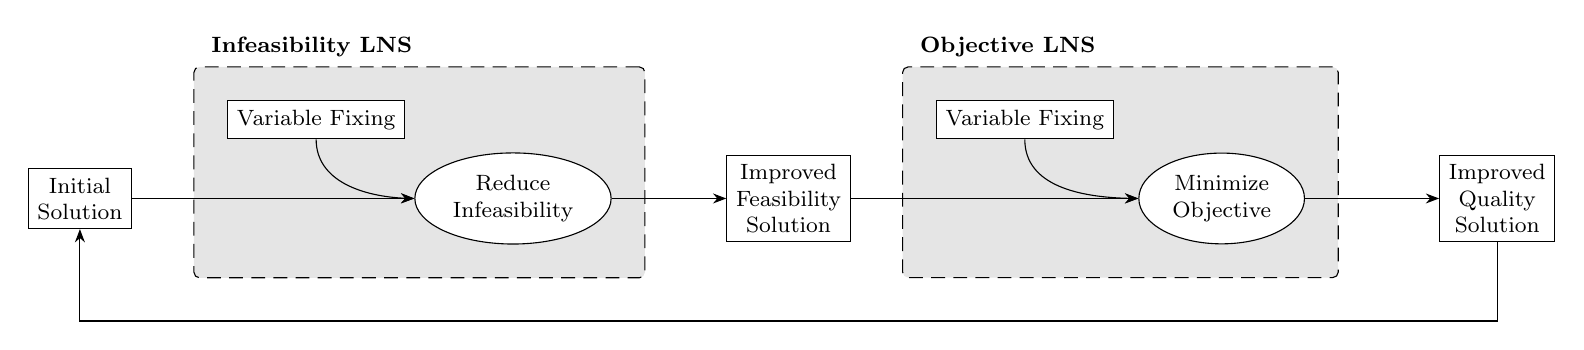
\begin{tikzpicture}[
    rect/.style={rectangle, draw=black, align=center, font=\footnotesize,fill=white},
    oval/.style={ellipse, draw=black, align=center, font=\footnotesize, fill=white},
    arrow/.style={->, >=Stealth},
    big-box/.style={rectangle, draw=black, dash pattern=on 5pt off 3pt,
                    inner sep=12pt, fill=gray!20, rounded corners=2pt},
    label/.style={font=\footnotesize\bfseries}
]

% ----------- Nodes (drawn first) -----------
% Initial Solution box
\node[rect] (initial) at (-3,0) {Initial\\Solution};

% Variable Fixing 1
\node[rect] (var-fix1) at (0,1) {Variable Fixing};

% Reduce Infeasibility
\node[oval] (reduce) at (2.5,0) {Reduce\\Infeasibility};

% Improved Feasible Solution
\node[rect] (improved-feas) at (6,0) {Improved\\Feasibility\\Solution};

% Variable Fixing 2
\node[rect] (var-fix2) at (9,1) {Variable Fixing};

% Minimize Objective
\node[oval] (minimize) at (11.5,0) {Minimize\\Objective};

% Improved Quality Solution
\node[rect] (improved-qual) at (15,0) {Improved\\Quality\\Solution};

% ----------- Background grouping boxes -----------
\begin{pgfonlayer}{background}
  \node[big-box, fit=(var-fix1)(reduce)] (infeas-box) {};
  \node[big-box, fit=(var-fix2)(minimize)] (obj-box) {};
\end{pgfonlayer}

% ----------- Labels (on top) -----------
\node[label, anchor=south west] at ([xshift=3pt]infeas-box.north west) {Infeasibility LNS};
\node[label, anchor=south west] at ([xshift=3pt]obj-box.north west) {Objective LNS};

% ----------- Arrows -----------
\draw[arrow] (initial.east) -- (reduce.west);
\draw[arrow] (var-fix1) to[out=-90,in=-180] (reduce);
\draw[arrow] (reduce.east) -- (improved-feas.west);
\draw[arrow] (improved-feas.east) -- (minimize.west);
\draw[arrow] (var-fix2) to[out=-90,in=-180] (minimize);
\draw[arrow] (minimize.east) -- (improved-qual.west);

% Feedback arrow
\draw[arrow] (improved-qual.south) -- ++(0,-1) -| (initial.south);

\end{tikzpicture}}
\caption{ACS Heuristic Workflow Diagram}
\label{fig:ACS_heu_workflow}
\end{figure}

\section{Feasibility-MIP (FMIP)}
In linear programming theory, it is well established that the feasibility problem can be addressed using the two-phase Simplex method, in which an auxiliary optimization problem is solved to obtain a feasible starting basis, and hence a feasible solution.
In a similar manner, the following auxiliary MIP problem, denoted as the Feasibility-MIP (FMIP), is formulated to identify a feasible starting solution:
\begin{equation}
\begin{cases}
\text{min} \quad & \sum_{i=0}^m \Delta_i^{+}+\Delta_i^{-} \\ \text{s.t.} \quad & Ax + I_m\Delta^+ - I_m\Delta^- =b\\ & x_i = \hat{x}_i, \; \forall i \in F\\ & l \le x \le u\\ & x_i \in \mathbb{Z}, \; \forall i \in \mathcal{I} \\ & \Delta^+ \ge 0, \Delta^- \ge 0 
\end{cases}
\end{equation}
Here, $I_m$ denotes an $m \times m$ identity matrix, while $\Delta^+$ and $\Delta^-$ are vectors in $R^m$ corresponding to the $m$ constraints. These are introduced as slack variables, and the objective is to minimize their sum. 
Analogous to the two-phase Simplex method, a vector $x$ is feasible for the original MIP if and only if it can be extended to a solution of value $0$ for the associated FMIP. Since solving an FMIP is as computationally demanding as solving the original problem, the neighborhoods are restricted by fixing a given subset $F$ of the integer variables to the values of an input vector $[\hat{x}, \Delta^+, \Delta^-]$. Because of the introduction of slack variables, the vector $\hat{x}$ is not required to be a feasible solution itself, but it must be integral and within the variable bounds to preserve the feasibility of the model. In this way, the FMIP guarantees that feasibility is preserved under any arbitrary variable-fixing scheme. Once a feasible solution is obtained, any LNS-based improving heuristic—such as RINS$^\text{\cite{RINS}}$, DINS$^\text{\cite{DINS}}$, or local branching$^\text{\cite{localBranching}}$—can then be applied to refine the solution.
\section{Optimality-MIP (OMIP)}
Rather than executing the FMIP until convergence to a feasible solution vector, the following auxiliary MIP problem, denoted as Optimality-MIP (OMIP), is designed to improve a partially feasible solution $[\hat{x}, \hat{\Delta}^+, \hat{\Delta}^-]$, which satisfies $\sum_{i=1}^m (\hat{\Delta}_i^+ + \hat{\Delta}_i^-) \neq 0$, with respect to the original objective $c^T x$:
\begin{equation}
\begin{cases}
\text{min} \quad & c^T x \\ \text{s.t.} \quad & Ax + I_m\Delta^+ - I_m\Delta^- = b\\ & \sum_{i=0}^m \Delta_i^{+}+\Delta_i^{-} \le \sum_{i=0}^m \hat\Delta_i^{+}+\hat\Delta_i^{-}\\ & x_i = \hat{x}_i, \; \forall i \in F\\ & l \le x \le u\\ & x_i \in \mathbb{Z},\; \forall i \in \mathcal{I} \\ & \Delta^+ \ge 0, \; \Delta^- \ge 0 
\end{cases}
\end{equation}
Analogous to the FMIP, the OMIP represents a reformulation of the original MIP model in which auxiliary slack variables are introduced for each constraint. This formulation enables the OMIP to enhance a solution even if it is not feasible for the original MIP. Moreover, to ensure that the optimal solution of the OMIP does not exceed the infeasibility of the input solution $\hat{x}$, an additional budget constraint is imposed, limiting the total slack to $\sum_{i=0}^m \hat\Delta_i^{+}+\hat\Delta_i^{-}$.

By iteratively solving subproblems of both auxiliary MIPs, the ACS heuristic is designed to converge—although convergence is not formally guaranteed—to a high-quality feasible solution. By construction, infeasibility decreases monotonically after each iteration. However, the quality of the solution with respect to the original objective function may fluctuate.

\section{Parallelization of ACS (PACS)}
The parallelization of ACS exploits parallelism by generating a diversified set of large neighborhood searches, which are solved simultaneously. Exploring multiple search neighborhoods in parallel is expected to increase the likelihood of identifying high-quality solutions.
Following this parallelization step, the improvements obtained in parallel must be combined efficiently. To this end, an additional search subproblem is generated in which variables with identical values across different solutions are fixed. Consequently, the recombination phase constitutes a crucial step in PACS: by merging the improvements achieved during the parallel phase, the subsequent phase can explore a newly diversified set of large neighborhood searches based on the recombined solution, thereby enhancing the probability of further improvements.
\begin{algorithm}[htbp]
\caption{Parallel Alternating Criteria Search (PACS)}\label{alg:PACS}
\begin{algorithmic}
\Function{FMIP\_LNS}{$MIP$, $F$, $\hat{x}$}
    \State \Return $\min\{\sum_i \Delta^+_i + \Delta^-_i \mid A x + I_m \Delta^+ - I_m \Delta^- = b, \; x_j = \hat{x}_j \; \forall j \in F, \; x_j \in \mathbb{Z} \; \forall j \in \mathcal{I}\}$
\EndFunction
\end{algorithmic}
\vspace{1em}
\begin{algorithmic}
\Function{OMIP\_LNS}{$MIP$, $F$, $\hat{x}$, $\hat{\Delta}$}
    \State \Return $\min\{c^T x \mid A x + I_m \Delta^+ - I_m \Delta^- = b, \; \sum_i^m \Delta^+_i + \Delta^-_i \leq \hat{\Delta}, \; x_j = \hat{x}_j \; \forall j \in F, \; x_j \in \mathbb{Z} \; \forall j \in \mathcal{I}\}$
\EndFunction
\end{algorithmic}
\vspace{1em}
\begin{algorithmic}[1]
\Require{Original $MIP$ formulation; PACS Execution time limit $TL_{PACS}$; Number of threads $T$; Initial solution parameter $\theta \in (0,100]$; Variable fixing parameter $\rho \in (0,1)$}
\Ensure{Feasible solution $\hat{x}$ if found}
\Function{PACS}{$MIP$, $TL_{PACS}$, $T$, $\theta$, $\rho$}
\State $[\hat{x}, \hat{\Delta}^+, \hat{\Delta}^-] \gets \Call{InitThetaSolution}{MIP,\theta,10^6}$
\While{\Call{TimeElapsed} $\le TL_{PACS}$ }
    \If{$\sum_i^m \hat\Delta_i^+ + \hat\Delta_i^- > 0$}
        \ForAll{threads $t_i:  i \in \{0,T-1\}$ \textbf{in parallel}}
            \State $F_{t_i} \gets \Call{RandomFixings}{MIP,\rho}$
            \State $[x^{t_i}, \Delta^{+t_i}, \Delta^{-t_i}] \gets \Call{FMIP\_LNS}{MIP,F_{t_i}, \hat{x}}$
        \EndFor
        \State $U \gets \{ j \in \mathcal{I} | x^{t_i}_j = x^{t_k}_j, \; 0 \leq i < k < T\}$
        \State $[\hat{x}, \hat{\Delta}^+, \hat{\Delta}^-] \gets \Call{FMIP\_LNS}{MIP,U, x^{t_0}}$
    \EndIf
    \State $\Delta^{UB} \gets \sum_i^m \hat{\Delta}_i^+ + \hat{\Delta}_i^-$
    \ForAll{threads $t_i:  i \in \{0,T-1\}$ \textbf{in parallel}}
            \State $F_{t_i} \gets \Call{RandomFixings}{MIP,\rho}$
            \State $[x^{t_i}, \Delta^{+t_i}, \Delta^{-t_i}] \gets \Call{OMIP\_LNS}{MIP,F_{t_i}, \hat{x}, \Delta^{UB}}$
    \EndFor
    \State $U \gets \{ j \in \mathcal{I} | x^{t_i}_j = x^{t_k}_j, \; 0 \leq i < k < T\}$
    \State $[\hat{x}, \hat{\Delta}^+, \hat{\Delta}^-] \gets \Call{OMIP\_LNS}{MIP,U, x^{t_0}, \Delta^{UB}}$
\EndWhile
\State \Return $[\hat{x}, \hat{\Delta}^+, \hat{\Delta}^-]$
\EndFunction
\end{algorithmic}
\end{algorithm}
The Algorithm \ref{alg:PACS} illustrates the overall workflow. In this process, each processor generates a set of randomized variable fixings and then solves the corresponding sub-MIP—either FMIP or OMIP—until the allotted time limit is reached.
Subsequently, the solutions are exchanged, and the set $U$, containing the indices of variables common across solutions, is constructed. The recombination MIP then consists of a subproblem, again associated with either FMIP or OMIP, in which the variables in $U$ are fixed.
The best solution obtained will be either the most feasible or the most optimal, depending on whether a recombination FMIP or OMIP is employed. Moreover, every solution used as input can be incorporated as a MIP start, as it remains feasible under any variable-fixing strategy.
Processor synchronization and memory communication are handled via the Message Passing Interface (MPI)$^\text{\cite{MPI}}$, owing to its efficient all-to-all collective communication primitives in distributed large-scale architectures.
To better illustrate the framework, Figure \ref{fig:PACS_heu_workflow} presents a schematic overview of the PACS heuristic, with an emphasis on its parallelization.
\begin{figure}[hbtp]
\centering
\resizebox{\columnwidth}{!}{
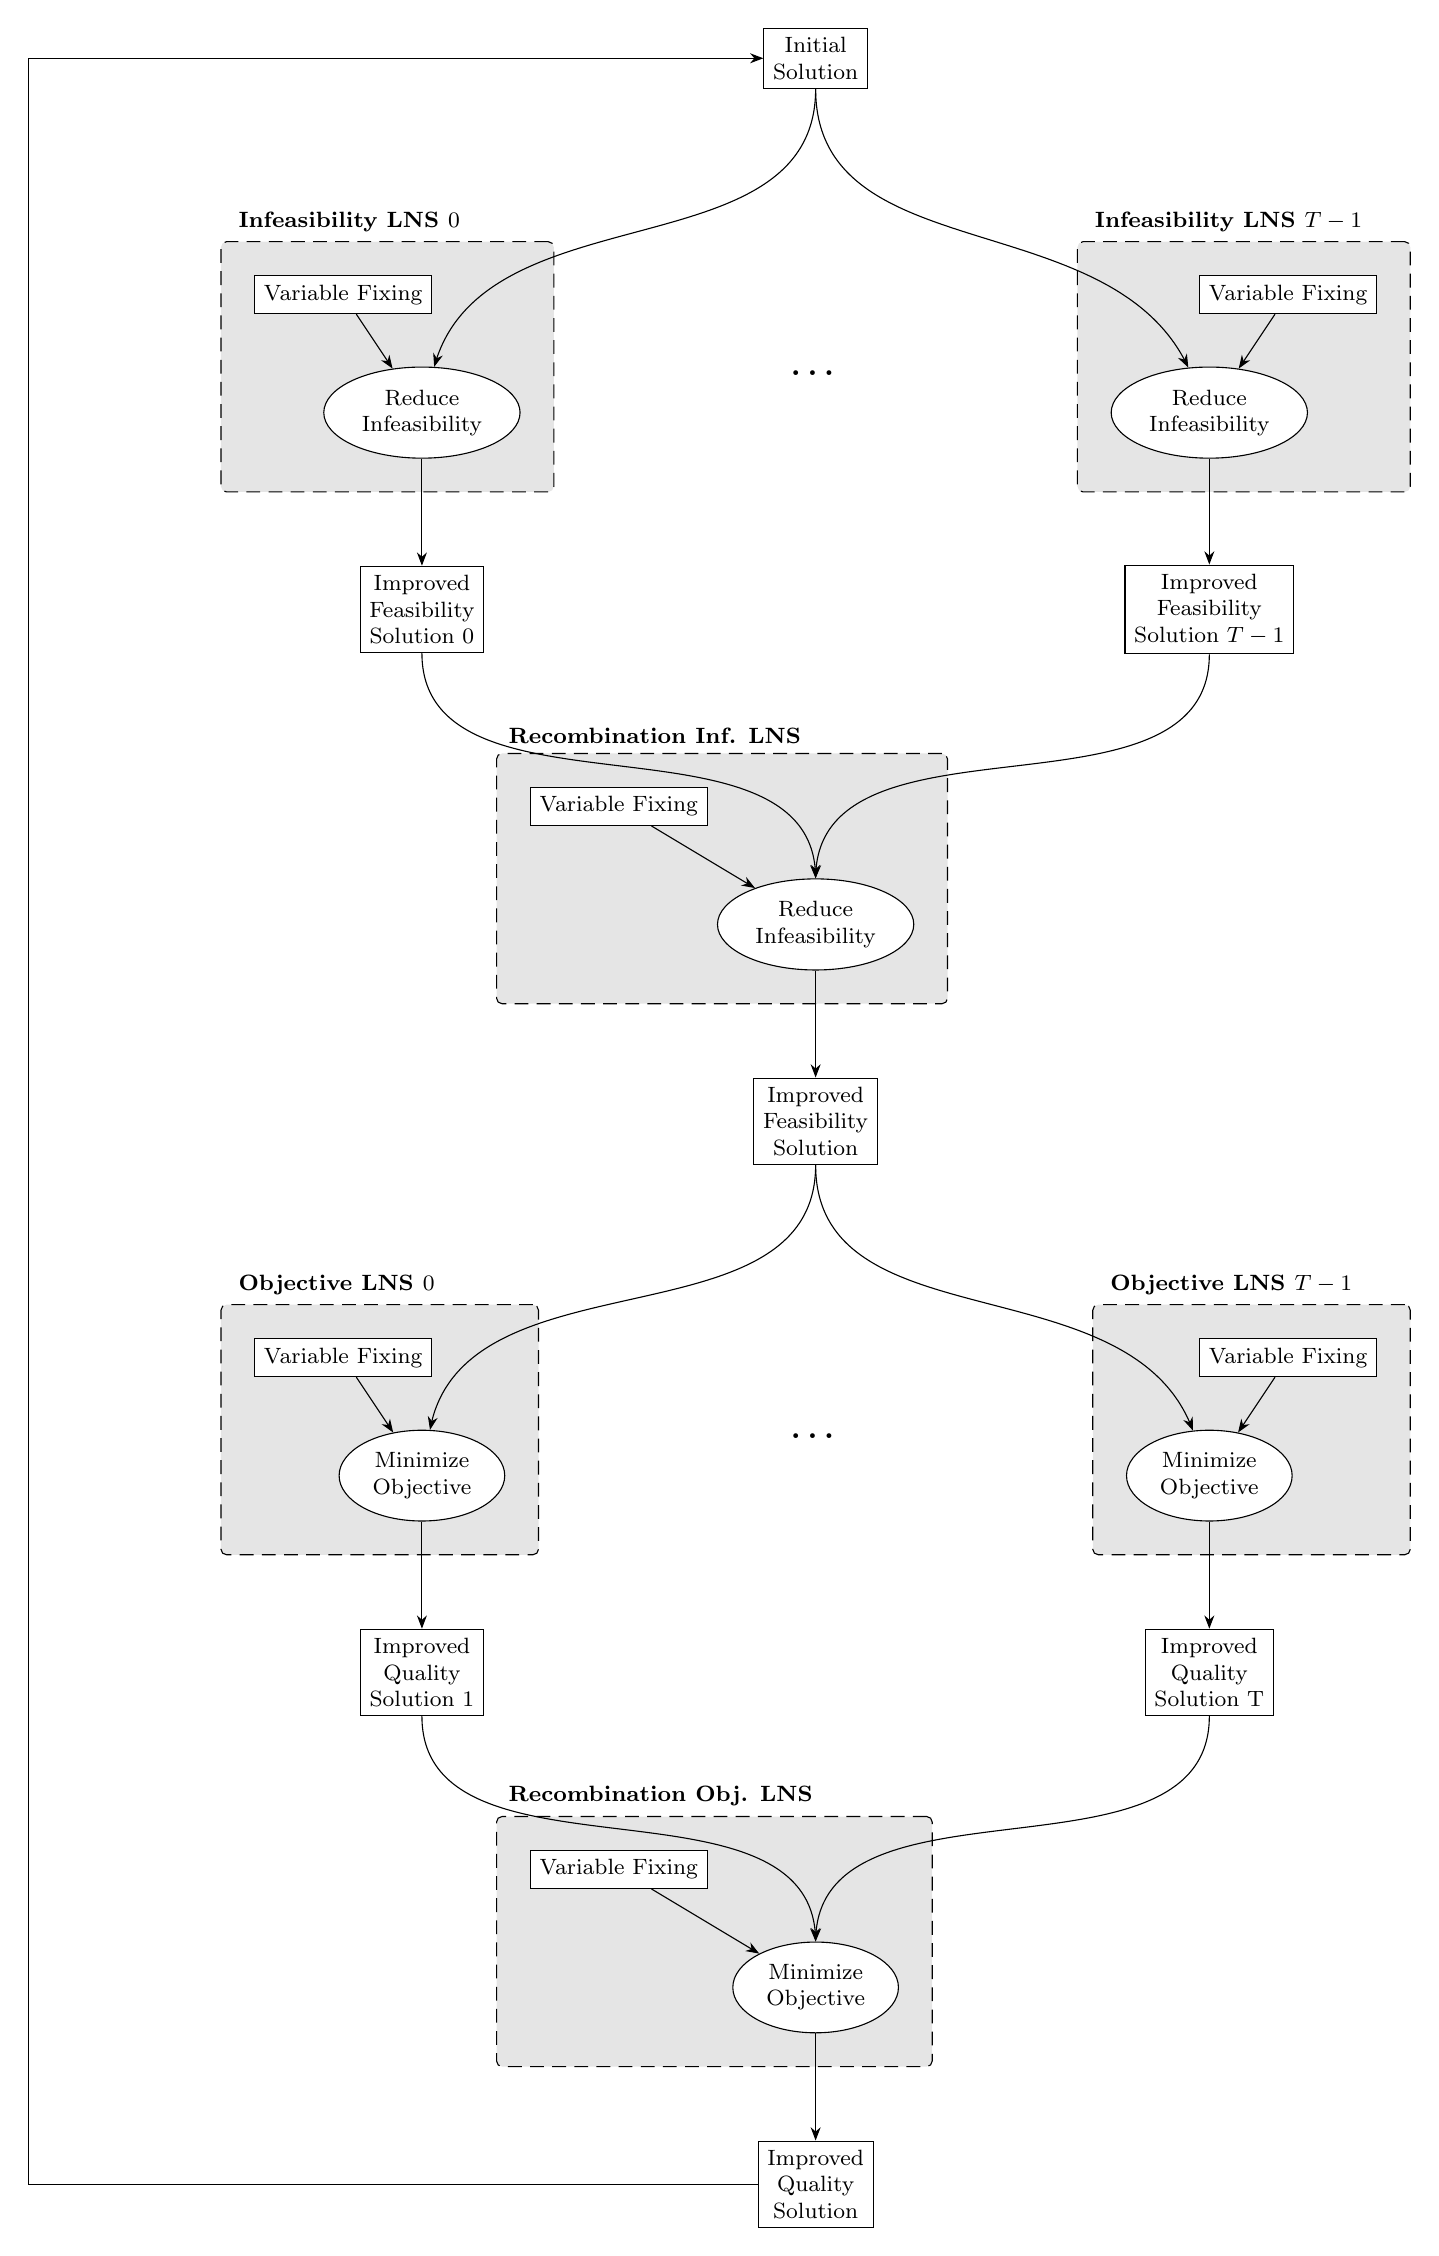
\begin{tikzpicture}[
    rect/.style={rectangle, draw=black, align=center, font=\footnotesize, fill=white},
    oval/.style={ellipse, draw=black, align=center, font=\footnotesize, fill=white},
    arrow/.style={->, >=Stealth},
    big-box/.style={rectangle, draw=black, dash pattern=on 5pt off 3pt,
                    inner sep=12pt, fill=gray!20, rounded corners=2pt},
    label/.style={font=\footnotesize\bfseries}
]

\node[rect] at (4,1) (initial) {Initial\\Solution};

\node[rect] at (-2,-2) (var_fix1) {Variable Fixing};
\node[rect] at (10,-2) (var_fixT) {Variable Fixing};
\node[oval] at (-1,-3.5) (reduce_infeas1) {Reduce \\ Infeasibility};
\node[oval] at (9,-3.5)  (reduce_infeasT) {Reduce \\ Infeasibility};

\node at (4,-3) (tmp){\large\textbf{\dots}};

\node[rect] at (-1,-6) (improved_feas1) {Improved\\Feasibility\\Solution $0$};
\node[rect] at (9,-6)  (improved_feasT) {Improved\\Feasibility\\Solution $T-1$};

\node[rect] at (1.5,-8.5) (var_fix_rFMIP) {Variable Fixing};
\node[oval] at (4,-10)  (infeas_rFMIP) {Reduce\\Infeasibility};
\node[rect] at (4,-12.5) (improved_rFMIP) {Improved\\Feasibility\\Solution};

\node[rect] at (-2,-15.5) (var_fix3) {Variable Fixing};
\node[rect] at (10,-15.5) (var_fixT2) {Variable Fixing};
\node[oval] at (-1,-17) (min_obj1) {Minimize\\Objective};
\node[oval] at (9,-17)  (min_objT) {Minimize\\Objective};

\node at (4,-16.5) (tmp2){\large\textbf{\dots}};

\node[rect] at (-1,-19.5) (improved_obj3) {Improved\\Quality\\Solution 1};
\node[rect] at (9,-19.5)  (improved_objT2) {Improved\\Quality\\Solution T};

\node[rect] at (1.5,-22) (var_fix_rOMIP) {Variable Fixing};
\node[oval] at (4,-23.5)  (min_obj_rOMIP) {Minimize\\Objective};
\node[rect] at (4,-26)  (improved_rOMIP) {Improved\\Quality\\Solution};

\begin{pgfonlayer}{background}

  \node[big-box, fit=(var_fix1)(reduce_infeas1)]  (infeas-box1) {};
  \node[big-box, fit=(var_fixT)(reduce_infeasT)]  (infeas-boxT) {};

  \node[big-box, fit=(var_fix_rFMIP)(infeas_rFMIP)] (rFMIP-box) {};

  \node[big-box, fit=(var_fix3)(min_obj1)]         (min_box_1) {};

  \node[big-box, fit=(var_fixT2)(min_objT)]        (min_box_T) {};

  \node[big-box, fit=(var_fix_rOMIP)(min_obj_rOMIP)] (rOMIP-box) {};
\end{pgfonlayer}

\node[label, anchor=south west] at ([xshift=3pt]infeas-box1.north west) {Infeasibility LNS $0$};

\node[label, anchor=south west] at ([xshift=3pt]infeas-boxT.north west) {Infeasibility LNS $T-1$};

\node[label, anchor=south west] at ([xshift=1pt]rFMIP-box.north west) {Recombination Inf. LNS};

\node[label, anchor=south west] at ([xshift=3pt]min_box_1.north west) {Objective LNS  $0$};
\node[label, anchor=south west] at ([xshift=3pt]min_box_T.north west) {Objective LNS $T-1$};

\node[label, anchor=south west] at ([xshift=1pt]rOMIP-box.north west) {Recombination Obj. LNS};

\draw[arrow] (var_fix1) -- (reduce_infeas1);
\draw[arrow] (initial) to[out=-90,in=75](reduce_infeas1);
\draw[arrow] (reduce_infeas1) -- (improved_feas1);


\draw[arrow] (var_fixT) -- (reduce_infeasT);
\draw[arrow] (initial) to[out=-90,in=115] (reduce_infeasT);
\draw[arrow] (reduce_infeasT) -- (improved_feasT);

\draw[arrow] (var_fix3) -- (min_obj1);
\draw[arrow] (min_obj1) -- (improved_obj3);
\draw[arrow] (improved_rFMIP) to[out=-90,in=80] (min_obj1);

\draw[arrow] (var_fixT2) -- (min_objT);
\draw[arrow] (min_objT) -- (improved_objT2);
\draw[arrow] (improved_rFMIP)  to[out=-90,in=110] (min_objT);

\draw[arrow] (improved_feas1) to[out=-90,in=90] (infeas_rFMIP);
\draw[arrow] (improved_feasT) to[out=-90,in=90] (infeas_rFMIP);
\draw[arrow] (var_fix_rFMIP) -- (infeas_rFMIP);
\draw[arrow] (infeas_rFMIP) -- (improved_rFMIP);

\draw[arrow] (improved_obj3)to[out=-90,in=90](min_obj_rOMIP);
\draw[arrow] (improved_objT2) to[out=-90,in=90] (min_obj_rOMIP);
\draw[arrow] (var_fix_rOMIP) -- (min_obj_rOMIP);
\draw[arrow] (min_obj_rOMIP) -- (improved_rOMIP);

\draw[arrow] (improved_rOMIP.west) -- (-6,-26) --(-6,1) -- (initial.west);

\end{tikzpicture}}
\caption{PACS Heuristic Workflow Diagram}\label{fig:PACS_heu_workflow}
\end{figure}

\section{Initialization of ACS}
As introduced earlier in this chapter, ACS only requires a starting vector that is integer feasible and within the variable bounds. However, a stronger starting point is a solution that is as feasible as possible with respect to the objective function of the FMIP.
The proposed algorithm provides a lightweight heuristic that seeks to minimize the infeasibility of the initial solution.
\begin{algorithm}
\caption{Starting vector heuristic}\label{alg:starting_vector}
\begin{algorithmic}
\Function{RELAXED\_FMIP}{$MIP$, $F$, $\hat{x}$}
    \State \Return $\min\{\sum_i \Delta_i^+ + \Delta_i^- \mid A x + I_m \Delta^+ - I_m \Delta^- = b, \; x_j = \hat{x}_j \;\; \forall j \in F\}$
\EndFunction
\end{algorithmic}
\vspace{1em}
\begin{algorithmic}[1]
\Require{Original $MIP$ formulation; Percentage of variables to fix $\theta \in (0,100]$; Fixed bound constant $c_b$}
\Ensure{Starting integer-feasible vector $\hat{x}$}
\Function{InitThetaSolution}{$MIP$, $\theta$, $c_b$}
\State $V \gets \text{sort}_\uparrow(\{x \in \mathcal{I}\}, (u_x-l_x))$
\State $F \gets \emptyset$
\State $\hat{x} \gets [+\infty, \ldots, +\infty] \in \bar{\mathbb{R}}^{n} $
\While{$\lnot \Call{IsIntegerFeasible}{\hat{x}} \land F \neq \mathcal{I}$}
    \State $\mathcal{K} \gets$ top $\theta \%$ of unfixed variables from $V$
    \For{$k \in \mathcal{K}$}
        \State $\hat{x}_k \gets \Call{RandomInteger}{\max(l_k, -c_b), \min(u_k, c_b)}$
    \EndFor
    \State $F \gets F \cup \mathcal{K}$
    \State $[x, \Delta^+, \Delta^-] \gets \Call{RELAXED\_FMIP}{MIP,F,\hat{x}}$
    \State $Q \gets \{i \;|\; x_i \in x,\; x_i \in \mathbb{Z},\; x_i \in \mathcal{I}\}$
    \State $\hat{x}_q \gets x_q, \; \forall q \in Q$
    \State $F \gets F \cup Q$
\EndWhile
\State \Return $\hat{x}$
\EndFunction
\end{algorithmic}
\end{algorithm}
The Algorithm \ref{alg:starting_vector} first sorts the list of integer variables in order of increasing bound range. It then fixes the top $\theta$\% of variables to random integer values within their respective bounds. The input parameter $\theta$ controls the trade-off between the difficulty of the LP relaxation and the quality of the resulting starting solution. In cases where the bounds are infinite, a constant value $c_b = 10^6$ is used to clamp the bounds.
The rationale behind the sorting step is to prioritize binary variables first, followed by the remaining integer variables.
Until all integer variables are fixed, the LP relaxation of the FMIP is solved to optimize the unfixed variables. Any variables that attain integer values in this process are then fixed.
Since at least $\theta$\% of the variables are fixed at each iteration, the algorithm is guaranteed to terminate after at most $\lceil 100 / \theta \rceil$ iterations.
\section{Variable Fixing Strategy}\label{sec:PACS_var_fix}
Selecting an appropriate variable fixing scheme is a challenging task: an overly restrictive strategy may fail to yield improvements, whereas an excessively loose strategy can lead to a search space that is too large to explore efficiently within a reasonable timespan.
The proposed algorithm constitutes a simple yet intuitive variable fixing method: it incorporates randomness to promote diversification and allows for controlling the number of variables to be fixed through an adjustable parameter.
\begin{algorithm}
\caption{Variable Fixing Selection Algorithm}\label{alg:variable_fixing}
\begin{algorithmic}[1]
\Require{Original $MIP$ formulation; Fraction of variables to fix $\rho \in (0,1)$}
\Ensure{Set of integer indices $F$}
\Function{RandomFixings}{$MIP$, $\rho$}
    \State $i \gets \Call{UniformFrom}{\mathcal{I}}$
    \State $F \gets \big[(i,i+1,\dots,i+\rho\cdot|\mathcal{I}| -1) \mod |\mathcal{I}|\big]$
    \State \Return $F$
\EndFunction
\end{algorithmic}
\end{algorithm}
In the Algorithm \ref{alg:variable_fixing}, the fixings are determined by selecting a random integer variable $x_i$ and fixing a consecutive sequence of integer variables starting from $x_i$ up to a cap determined by $\rho$, an input parameter that specifies the number of variables to be fixed.
The fixing is performed in a circular fashion: if the end of the set $\mathcal{I}$ is reached before the required number of variables are fixed, the algorithm continues from the beginning of $\mathcal{I}$.
The effectiveness of this strategy relies on the fact that, for many problems—such as network flow and routing—the variables are arranged consecutively, often defining a cohesive substructure within the problem.

%\afterpage{\blankpage}

% % Chapter 2
\clearpage{\pagestyle{plain}\cleardoublepage}
\chapter{The PACS Tuning}
As discussed in the section[\ref{sec:lim_PACS}], the baseline PACS has a some limitations that make it not suitable for the general-purpose environments. Hence, the PACS parameter and PACS itself are tuned up with this aim: make PACS hardware and input independent, in order to be embedded into a state-of-the-art MIP solver-such as IBM ILOG CPLEX or GUROBI-.
% Parameter to tune up: theta, rho, timing 

\section{PACS with Generalized Fixing}
The baseline PACS algorithm enforces both the starting vector construction and the fixing scheme to operate exclusively on the set $\mathcal{I}$ of integer variables. While this restriction may appear efficient and straightforward, it can, in fact, be limiting. In particular, if the MIP instance contains only a small fraction of integer variables relative to the total, focusing solely on them may reduce diversification and cause the algorithm to converge prematurely to a local minimum, which is undesirable in an optimization process.
To overcome this issue, algorithm[\ref{alg:starting_vector}] and algorithm[\ref{alg:variable_fixing}] are generalized into algorithm[\ref{alg:gen_starting_vector}] and algorithm[\ref{alg:gen_variable_fixing}], respectively, thereby allowing both integer and continuous variables to be considered.
\begin{algorithm}[H]
\caption{Generalized Starting vector heuristic}\label{alg:gen_starting_vector}
\begin{algorithmic}[1]
\Require{Percentage of variables to fix $\theta$, $0 < \theta \leq 100$, Fixed bound constant $c_b$}
\Ensure{Starting integer-feasible vector $\hat{x}$}
\State $V :=$ list of \cancel{integer} variables sorted by increasing bound range $u-l$
\State $F := \emptyset$
\While{$\hat{x}$ is not integer feasible \textbf{AND} $F \neq V$}
    \State $\mathcal{K} :=$ top $\theta \%$ of unfixed variables from $V$
    \For{$k \in \mathcal{K}$}
        \State $\hat{x}_k :=$ random integer value between $[\max(l_k, -c_b), \min(u_k, c_b)]$
    \EndFor
    \State $F := F \cup \mathcal{K}$
    \State $[x, \Delta^+, \Delta^-] := \min\{\sum_i \Delta_i^+ + \Delta_i^- \mid A x + I_m \Delta^+ - I_m \Delta^- = b, \; x_j = \hat{x}_j \;\; \forall j \in F\}$
    \State $Q :=$ index set of \cancel{integer} variables of $x$ with integer value
    \State $\hat{x}_q = x_q, \;\; \forall q \in Q$
    \State $F := F \cup Q$
\EndWhile
\State \Return $\hat{x}$
\end{algorithmic}
\end{algorithm}
\begin{algorithm}[H]
\caption{Generalized Variable Fixing Selection Algorithm}\label{alg:gen_variable_fixing}
\begin{algorithmic}[1]
\Require{Fraction of variables to fix $\rho$, $0 < \rho < 1$}
\Ensure{Set of integer indices $F$}
\Function{RandomFixings}{$\rho$}
    \State $i :=$ random element in $\{1\dots n\}$ \Comment $n$: number of variables in the original MIP 
    \State $F :=$ first $\rho \cdot n$ consecutive \cancel{integer} variable indices starting from $i$ in a circular fashion
    \State \Return $F$
\EndFunction
\end{algorithmic}
\end{algorithm}
Since these algorithms are executed on the auxiliary MIP problems -FMIP or OMIP-, the variables subject to fixing correspond exactly to those defined in the original MIP formulation.  
By generalizing the fixing strategy to include both integer and continuous variables, diversification is enhanced, thereby reducing the likelihood of stagnation in local minima and potentially improving the exploration of the solution space.

\section{Architecture-Agnostic Parallelization}
In the original study, the Message Passing Interface (MPI) was employed to synchronize processors at each recombination phase. While this approach is well suited to high-performance computing environments, it may be unnecessarily complex in general-purpose scenarios, where a simpler multi-threading implementation is often preferable.  
In this thesis, communication is instead managed through a set of logical threads, which may differ from the number of available hardware threads. This abstraction ensures that, even on machines with fewer physical cores, the algorithm can reproduce the same behavior across different architectures, provided sufficient computational time is allowed.  
More specifically, during the coordination phase, either the most feasible or the most optimal solution—depending on whether a recombination FMIP or OMIP is performed—is shared among the logical processors. Each processor then continues working independently on its own copy, with updates to the incumbent solution handled exclusively through a thread-safe update function.  
\begin{algorithm}[H]
\caption{Parallel ACS Incumbent Update Procedure}
\begin{algorithmic}[1]
\Require Candidate solution $x$ with slack sum $S(x)$ and objective value $C(x)$; Incumbent $\tilde{x}$; Zero-tolerance $\epsilon$
\Ensure Updated incumbent $\tilde{x}$ in a thread-safe manner
\Function{UpdateIncumbent}{$x$}
    \State acquire lock
    \If{$(|S(x)| < |S(\tilde{x})|) \;\;\lor\;\; (|S(x)| < \epsilon \;\land\; C(x) < C(\tilde{x}))$}
        \State $\tilde{x} \gets x$
    \EndIf
    \State release lock
\EndFunction
\end{algorithmic}
\end{algorithm}

This mechanism is crucial to ensure that the algorithm consistently improves and converges within the given time limit. The incumbent solution is updated whenever a better solution is identified: either one with a smaller total slack, indicating improved feasibility, or one with a lower objective value $c^T x$ provided that the slack sum is less than the tolerance parameter $\epsilon$, the zero-feasibility threshold.

\section{Parameter Tuning without an Explicit Calibration Phase}
To eliminate the need for a separate calibration phase, the parameters $\theta$ for the starting vector, $\rho$ for the fixing strategy, and the time span of each sub-MIP in Algorithm \ref{alg:PACS} must be carefully selected.  
\subsection{Determination of Parameter $\theta$}
For simplicity, the parameter $\theta$ is initially fixed to $0.25$. A more effective initialization strategy will be discussed in the Section \ref{}, where a new heuristic is introduced.  
\subsection{Determination of Sub-MIP Time Limit}
To ensure determinism in the implementation, each sub-MIP is assigned both a time limit equal to the remaining computation time and a deterministic time limit, defined as the maximum number of instructions the solver can execute before termination.  
The deterministic time limit is set according to the following formula:
$$
TL_{DET} = \max\Big(x, \min\Big(\frac{nz}{y}, X\Big)\Big),
$$
which provides a dynamic strategy to determine the deterministic time limit of the sub-MIP.  
Here, $x$ and $X$ denote the minimum and maximum allowable values for the deterministic time limit, respectively, $nz$ represents the number of nonzeros in the constraint matrix $A$ of the MIP problem, and $y$ serves as a scaling factor. The selected parameter values are as follows:
\begin{enumerate}
\item Minimum deterministic time limit: $x = 10^3$  
\item Scaling factor: $y = 10^2$  
\item Maximum deterministic time limit: $X = 10^7$  
\end{enumerate}
\subsection{Determination of Parameter $\rho$}
The parameter $\rho$ is chosen from the set $\{0.1, 0.25, 0.5, 0.75, 0.9\}$ based on experimental results. Further details are provided in Chapter \ref{}. Intuitively, a smaller value of $\rho$ offers greater flexibility to the solver, which can improve the quality of the intermediate solutions.  

\section{Dynamic Fixing Strategy}



% %\afterpage{\blankpage}

% % Chapter 3
\clearpage{\pagestyle{plain}\cleardoublepage}
\chapter{Experimental Results}
%intro
\section{Experimental Setup}
The experiments are designed to compare the PACS framework with the standalone IBM ILOG CPLEX Optimization Studio (version 22.1).  
The PACS framework is implemented in C++ for performance reasons, interfacing with the solver through the C API. The source code is available under a non-commercial MIP license at \textbf{[repository link]}.  
All experiments were conducted on a cluster within the UniPD DEI Blade infrastructure, running Rocky Linux 8.10. Each node is equipped with an Intel(R) Xeon(R) E5-2623 v3 processor (4 cores, 3.00 GHz) and 16 GB of RAM. Although the infrastructure is cluster-based, the computational power of a single node is comparable to that of a general-purpose laptop, or even lower.  
For fairness in comparison, PACS executions use 4 logical threads, implemented as C++ standard threads, each running a CPLEX instance restricted to a single core. The baseline counterpart is a standalone CPLEX execution restricted to 4 cores.

\subsection{Dataset}
As anticipated in the previous sections, the benchmark for this comparison must consist of hard MIP instances. To this end, the set of hard instances from MIPLIB2017$^\text{\cite{MIPLIB}}$ has been used as the test bed.\footnote{The instance \textit{tpl-tub-ss16} was excluded, as its execution was terminated due to insufficient computational resources.}  
While CPLEX directly processes each MIP instance, the PACS framework additionally requires a random seed in order to reproduce the same randomized choices across different runs. For this purpose, PACS was evaluated on each instance using the seeds $\{38472910, 56473829, 27384910, 91827364, 8374659\}$. This setup increases statistical reliability and can be considered representative of the algorithm’s standard behavior.  
Consequently, for each instance, five independent PACS runs and one CPLEX run were executed.

\subsection{Metrics}
Both PACS and plain CPLEX terminate as soon as an incumbent solution (i.e., a feasible solution) is identified, subject to a global time limit of five minutes.
Since the PACS framework was executed five times for each instance, the reported solution quality and computation time are given as the mean across all runs.
Moreover, if the majority of PACS executions for a given instance---at least three out of five seeds---fail to produce a solution, the instance is recorded as unsolved.
Instead of directly comparing the objective values of the solutions returned by the two approaches, the MIP gap metric$^\text{\cite{MIPGAP}}$ has been adopted. The MIP gap is defined as follows: given a solution $\hat{x}$ for a MIP with an optimal solution $x$, the primal gap $\gamma(\hat{x}) \in [0,1]$ is
\begin{equation}
\gamma(\hat{x}) =
\begin{cases}
0 & \text{if } |c^T x| = |c^T \hat{x}| = 0, \\
1 & \text{if } c^T x \cdot c^T \hat{x}< 0, \\
\frac{|c^T x-c^T \hat{x}|}{\max\{|c^T \hat{x}|, |c^T x|\}} & \text{otherwise}.
\end{cases}
\end{equation}
This metric captures the relative gap between an incumbent and the best-known solution, normalized to the interval $[0,1]$.  
Since the algorithms operate under a strict time limit, the metric must be extended accordingly. Given a time limit $t_{\max}$, the primal function $p:[0,t_{\max}] \to [0,1]$ is defined as:
\begin{equation}
p(\hat{x}) =
\begin{cases}
1 & \text{if no solution is found up to time $t$}, \\
\gamma(\hat{x}(t)) & \text{if $\hat{x}(t)$ is the incumbent at time $t$}.
\end{cases}
\end{equation}
For each test, two types of plots are produced to summarize and compare performance:
\begin{enumerate}
    \item \textbf{Success Rate vs. Computation Time:}  
    The $x$-axis represents elapsed time, and the $y$-axis reports the cumulative number of instances for which an incumbent was found. The closer a curve is to the top-left corner, the more efficient the algorithm.  
    \item \textbf{Success Rate vs. MIP Gap:}  
    The $x$-axis represents the MIP gap, and the $y$-axis reports the cumulative number of instances solved with a gap less than or equal to the given value. Consistently, curves closer to the top-left corner indicate better performance 
\end{enumerate}
To provide a more compact quantitative comparison, the integral of each curve has been computed and reported in a corresponding bar chart, one for each plot.

\subsection{Tolerance Parameters}
Because both algorithms involve floating-point computations and comparisons, PACS employs a set of tolerance parameters. In these experiments, the parameters were selected to be reasonable relative to the defaults used by CPLEX:
\begin{itemize}
    \item \textbf{Zero-tolerance parameter} $\epsilon$: values smaller than $\epsilon$ are treated as zero. In all tests, $\epsilon$ was set to $10^{-5}$.
    \item \textbf{Absolute maximum constraint violation}: the maximum permissible violation of any constraint under a candidate solution $\hat{x}$. In these tests, it was set equal to $\epsilon$, i.e., $10^{-5}$.
    \item \textbf{Absolute maximum integrality violation}: the maximum deviation allowed for variables constrained to take integer values. This tolerance was likewise set to $\epsilon = 10^{-5}$.
    \item \textbf{Relative objective error}: the maximum admissible relative error between the recomputed objective value $c^T \hat{x}$ and the value stored internally by PACS. This threshold was again set to $\epsilon = 10^{-5}$.  
\end{itemize}  
In the latter three cases, if the corresponding tolerance is exceeded, the algorithm terminates with an error and the run is recorded as unsolved.  

\section{Results}
This section presents the experimental evaluation and details the progressive tuning of PACS parameters. Each test builds upon the outcomes of the previous one, providing a stepwise refinement of the algorithm.

\subsection{Fixed $\rho$ Initialization Test}\label{sec:test_fix_rho}
The first experiment focuses on the choice of the parameter $\rho$ in the variable-fixing strategy.  
In this experiment, PACS was employed with generalized fixing strategies under an architecture-agnostic parallelization scheme
The predefined values of $\rho$ considered are $\{.1, .25, .5, .75, .9\}$.  
It is worth noting that smaller values of $\rho$ leave greater freedom to the MIP solver.  

Since the PACS algorithm also requires the parameter $\theta$ for the initial solution construction strategy, it was fixed to $\theta = .25$ for this test.  

\begin{figure}[H]
    \centering
    \begin{minipage}{0.6\columnwidth}
        \centering
        \resizebox{\linewidth}{!}{%% Creator: Matplotlib, PGF backend
%%
%% To include the figure in your LaTeX document, write
%%   \input{<filename>.pgf}
%%
%% Make sure the required packages are loaded in your preamble
%%   \usepackage{pgf}
%%
%% Also ensure that all the required font packages are loaded; for instance,
%% the lmodern package is sometimes necessary when using math font.
%%   \usepackage{lmodern}
%%
%% Figures using additional raster images can only be included by \input if
%% they are in the same directory as the main LaTeX file. For loading figures
%% from other directories you can use the `import` package
%%   \usepackage{import}
%%
%% and then include the figures with
%%   \import{<path to file>}{<filename>.pgf}
%%
%% Matplotlib used the following preamble
%%   \def\mathdefault#1{#1}
%%   \everymath=\expandafter{\the\everymath\displaystyle}
%%   \IfFileExists{scrextend.sty}{
%%     \usepackage[fontsize=10.000000pt]{scrextend}
%%   }{
%%     \renewcommand{\normalsize}{\fontsize{10.000000}{12.000000}\selectfont}
%%     \normalsize
%%   }
%%   
%%   \ifdefined\pdftexversion\else  % non-pdftex case.
%%     \usepackage{fontspec}
%%     \setmainfont{DejaVuSerif.ttf}[Path=\detokenize{/home/bisca/.global/lib/python3.12/site-packages/matplotlib/mpl-data/fonts/ttf/}]
%%     \setsansfont{DejaVuSans.ttf}[Path=\detokenize{/home/bisca/.global/lib/python3.12/site-packages/matplotlib/mpl-data/fonts/ttf/}]
%%     \setmonofont{DejaVuSansMono.ttf}[Path=\detokenize{/home/bisca/.global/lib/python3.12/site-packages/matplotlib/mpl-data/fonts/ttf/}]
%%   \fi
%%   \makeatletter\@ifpackageloaded{underscore}{}{\usepackage[strings]{underscore}}\makeatother
%%
\begingroup%
\makeatletter%
\begin{pgfpicture}%
\pgfpathrectangle{\pgfpointorigin}{\pgfqpoint{12.000000in}{8.000000in}}%
\pgfusepath{use as bounding box, clip}%
\begin{pgfscope}%
\pgfsetbuttcap%
\pgfsetmiterjoin%
\definecolor{currentfill}{rgb}{1.000000,1.000000,1.000000}%
\pgfsetfillcolor{currentfill}%
\pgfsetlinewidth{0.000000pt}%
\definecolor{currentstroke}{rgb}{1.000000,1.000000,1.000000}%
\pgfsetstrokecolor{currentstroke}%
\pgfsetdash{}{0pt}%
\pgfpathmoveto{\pgfqpoint{0.000000in}{0.000000in}}%
\pgfpathlineto{\pgfqpoint{12.000000in}{0.000000in}}%
\pgfpathlineto{\pgfqpoint{12.000000in}{8.000000in}}%
\pgfpathlineto{\pgfqpoint{0.000000in}{8.000000in}}%
\pgfpathlineto{\pgfqpoint{0.000000in}{0.000000in}}%
\pgfpathclose%
\pgfusepath{fill}%
\end{pgfscope}%
\begin{pgfscope}%
\pgfsetbuttcap%
\pgfsetmiterjoin%
\definecolor{currentfill}{rgb}{1.000000,1.000000,1.000000}%
\pgfsetfillcolor{currentfill}%
\pgfsetlinewidth{0.000000pt}%
\definecolor{currentstroke}{rgb}{0.000000,0.000000,0.000000}%
\pgfsetstrokecolor{currentstroke}%
\pgfsetstrokeopacity{0.000000}%
\pgfsetdash{}{0pt}%
\pgfpathmoveto{\pgfqpoint{0.661528in}{0.586684in}}%
\pgfpathlineto{\pgfqpoint{11.811750in}{0.586684in}}%
\pgfpathlineto{\pgfqpoint{11.811750in}{7.850000in}}%
\pgfpathlineto{\pgfqpoint{0.661528in}{7.850000in}}%
\pgfpathlineto{\pgfqpoint{0.661528in}{0.586684in}}%
\pgfpathclose%
\pgfusepath{fill}%
\end{pgfscope}%
\begin{pgfscope}%
\pgfpathrectangle{\pgfqpoint{0.661528in}{0.586684in}}{\pgfqpoint{11.150222in}{7.263316in}}%
\pgfusepath{clip}%
\pgfsetbuttcap%
\pgfsetroundjoin%
\pgfsetlinewidth{0.803000pt}%
\definecolor{currentstroke}{rgb}{0.690196,0.690196,0.690196}%
\pgfsetstrokecolor{currentstroke}%
\pgfsetstrokeopacity{0.500000}%
\pgfsetdash{{2.960000pt}{1.280000pt}}{0.000000pt}%
\pgfpathmoveto{\pgfqpoint{2.408396in}{0.586684in}}%
\pgfpathlineto{\pgfqpoint{2.408396in}{7.850000in}}%
\pgfusepath{stroke}%
\end{pgfscope}%
\begin{pgfscope}%
\pgfsetbuttcap%
\pgfsetroundjoin%
\definecolor{currentfill}{rgb}{0.000000,0.000000,0.000000}%
\pgfsetfillcolor{currentfill}%
\pgfsetlinewidth{0.803000pt}%
\definecolor{currentstroke}{rgb}{0.000000,0.000000,0.000000}%
\pgfsetstrokecolor{currentstroke}%
\pgfsetdash{}{0pt}%
\pgfsys@defobject{currentmarker}{\pgfqpoint{0.000000in}{-0.048611in}}{\pgfqpoint{0.000000in}{0.000000in}}{%
\pgfpathmoveto{\pgfqpoint{0.000000in}{0.000000in}}%
\pgfpathlineto{\pgfqpoint{0.000000in}{-0.048611in}}%
\pgfusepath{stroke,fill}%
}%
\begin{pgfscope}%
\pgfsys@transformshift{2.408396in}{0.586684in}%
\pgfsys@useobject{currentmarker}{}%
\end{pgfscope}%
\end{pgfscope}%
\begin{pgfscope}%
\definecolor{textcolor}{rgb}{0.000000,0.000000,0.000000}%
\pgfsetstrokecolor{textcolor}%
\pgfsetfillcolor{textcolor}%
\pgftext[x=2.408396in,y=0.489462in,,top]{\color{textcolor}{\rmfamily\fontsize{10.000000}{12.000000}\selectfont\catcode`\^=\active\def^{\ifmmode\sp\else\^{}\fi}\catcode`\%=\active\def%{\%}50}}%
\end{pgfscope}%
\begin{pgfscope}%
\pgfpathrectangle{\pgfqpoint{0.661528in}{0.586684in}}{\pgfqpoint{11.150222in}{7.263316in}}%
\pgfusepath{clip}%
\pgfsetbuttcap%
\pgfsetroundjoin%
\pgfsetlinewidth{0.803000pt}%
\definecolor{currentstroke}{rgb}{0.690196,0.690196,0.690196}%
\pgfsetstrokecolor{currentstroke}%
\pgfsetstrokeopacity{0.500000}%
\pgfsetdash{{2.960000pt}{1.280000pt}}{0.000000pt}%
\pgfpathmoveto{\pgfqpoint{4.266766in}{0.586684in}}%
\pgfpathlineto{\pgfqpoint{4.266766in}{7.850000in}}%
\pgfusepath{stroke}%
\end{pgfscope}%
\begin{pgfscope}%
\pgfsetbuttcap%
\pgfsetroundjoin%
\definecolor{currentfill}{rgb}{0.000000,0.000000,0.000000}%
\pgfsetfillcolor{currentfill}%
\pgfsetlinewidth{0.803000pt}%
\definecolor{currentstroke}{rgb}{0.000000,0.000000,0.000000}%
\pgfsetstrokecolor{currentstroke}%
\pgfsetdash{}{0pt}%
\pgfsys@defobject{currentmarker}{\pgfqpoint{0.000000in}{-0.048611in}}{\pgfqpoint{0.000000in}{0.000000in}}{%
\pgfpathmoveto{\pgfqpoint{0.000000in}{0.000000in}}%
\pgfpathlineto{\pgfqpoint{0.000000in}{-0.048611in}}%
\pgfusepath{stroke,fill}%
}%
\begin{pgfscope}%
\pgfsys@transformshift{4.266766in}{0.586684in}%
\pgfsys@useobject{currentmarker}{}%
\end{pgfscope}%
\end{pgfscope}%
\begin{pgfscope}%
\definecolor{textcolor}{rgb}{0.000000,0.000000,0.000000}%
\pgfsetstrokecolor{textcolor}%
\pgfsetfillcolor{textcolor}%
\pgftext[x=4.266766in,y=0.489462in,,top]{\color{textcolor}{\rmfamily\fontsize{10.000000}{12.000000}\selectfont\catcode`\^=\active\def^{\ifmmode\sp\else\^{}\fi}\catcode`\%=\active\def%{\%}100}}%
\end{pgfscope}%
\begin{pgfscope}%
\pgfpathrectangle{\pgfqpoint{0.661528in}{0.586684in}}{\pgfqpoint{11.150222in}{7.263316in}}%
\pgfusepath{clip}%
\pgfsetbuttcap%
\pgfsetroundjoin%
\pgfsetlinewidth{0.803000pt}%
\definecolor{currentstroke}{rgb}{0.690196,0.690196,0.690196}%
\pgfsetstrokecolor{currentstroke}%
\pgfsetstrokeopacity{0.500000}%
\pgfsetdash{{2.960000pt}{1.280000pt}}{0.000000pt}%
\pgfpathmoveto{\pgfqpoint{6.125137in}{0.586684in}}%
\pgfpathlineto{\pgfqpoint{6.125137in}{7.850000in}}%
\pgfusepath{stroke}%
\end{pgfscope}%
\begin{pgfscope}%
\pgfsetbuttcap%
\pgfsetroundjoin%
\definecolor{currentfill}{rgb}{0.000000,0.000000,0.000000}%
\pgfsetfillcolor{currentfill}%
\pgfsetlinewidth{0.803000pt}%
\definecolor{currentstroke}{rgb}{0.000000,0.000000,0.000000}%
\pgfsetstrokecolor{currentstroke}%
\pgfsetdash{}{0pt}%
\pgfsys@defobject{currentmarker}{\pgfqpoint{0.000000in}{-0.048611in}}{\pgfqpoint{0.000000in}{0.000000in}}{%
\pgfpathmoveto{\pgfqpoint{0.000000in}{0.000000in}}%
\pgfpathlineto{\pgfqpoint{0.000000in}{-0.048611in}}%
\pgfusepath{stroke,fill}%
}%
\begin{pgfscope}%
\pgfsys@transformshift{6.125137in}{0.586684in}%
\pgfsys@useobject{currentmarker}{}%
\end{pgfscope}%
\end{pgfscope}%
\begin{pgfscope}%
\definecolor{textcolor}{rgb}{0.000000,0.000000,0.000000}%
\pgfsetstrokecolor{textcolor}%
\pgfsetfillcolor{textcolor}%
\pgftext[x=6.125137in,y=0.489462in,,top]{\color{textcolor}{\rmfamily\fontsize{10.000000}{12.000000}\selectfont\catcode`\^=\active\def^{\ifmmode\sp\else\^{}\fi}\catcode`\%=\active\def%{\%}150}}%
\end{pgfscope}%
\begin{pgfscope}%
\pgfpathrectangle{\pgfqpoint{0.661528in}{0.586684in}}{\pgfqpoint{11.150222in}{7.263316in}}%
\pgfusepath{clip}%
\pgfsetbuttcap%
\pgfsetroundjoin%
\pgfsetlinewidth{0.803000pt}%
\definecolor{currentstroke}{rgb}{0.690196,0.690196,0.690196}%
\pgfsetstrokecolor{currentstroke}%
\pgfsetstrokeopacity{0.500000}%
\pgfsetdash{{2.960000pt}{1.280000pt}}{0.000000pt}%
\pgfpathmoveto{\pgfqpoint{7.983507in}{0.586684in}}%
\pgfpathlineto{\pgfqpoint{7.983507in}{7.850000in}}%
\pgfusepath{stroke}%
\end{pgfscope}%
\begin{pgfscope}%
\pgfsetbuttcap%
\pgfsetroundjoin%
\definecolor{currentfill}{rgb}{0.000000,0.000000,0.000000}%
\pgfsetfillcolor{currentfill}%
\pgfsetlinewidth{0.803000pt}%
\definecolor{currentstroke}{rgb}{0.000000,0.000000,0.000000}%
\pgfsetstrokecolor{currentstroke}%
\pgfsetdash{}{0pt}%
\pgfsys@defobject{currentmarker}{\pgfqpoint{0.000000in}{-0.048611in}}{\pgfqpoint{0.000000in}{0.000000in}}{%
\pgfpathmoveto{\pgfqpoint{0.000000in}{0.000000in}}%
\pgfpathlineto{\pgfqpoint{0.000000in}{-0.048611in}}%
\pgfusepath{stroke,fill}%
}%
\begin{pgfscope}%
\pgfsys@transformshift{7.983507in}{0.586684in}%
\pgfsys@useobject{currentmarker}{}%
\end{pgfscope}%
\end{pgfscope}%
\begin{pgfscope}%
\definecolor{textcolor}{rgb}{0.000000,0.000000,0.000000}%
\pgfsetstrokecolor{textcolor}%
\pgfsetfillcolor{textcolor}%
\pgftext[x=7.983507in,y=0.489462in,,top]{\color{textcolor}{\rmfamily\fontsize{10.000000}{12.000000}\selectfont\catcode`\^=\active\def^{\ifmmode\sp\else\^{}\fi}\catcode`\%=\active\def%{\%}200}}%
\end{pgfscope}%
\begin{pgfscope}%
\pgfpathrectangle{\pgfqpoint{0.661528in}{0.586684in}}{\pgfqpoint{11.150222in}{7.263316in}}%
\pgfusepath{clip}%
\pgfsetbuttcap%
\pgfsetroundjoin%
\pgfsetlinewidth{0.803000pt}%
\definecolor{currentstroke}{rgb}{0.690196,0.690196,0.690196}%
\pgfsetstrokecolor{currentstroke}%
\pgfsetstrokeopacity{0.500000}%
\pgfsetdash{{2.960000pt}{1.280000pt}}{0.000000pt}%
\pgfpathmoveto{\pgfqpoint{9.841877in}{0.586684in}}%
\pgfpathlineto{\pgfqpoint{9.841877in}{7.850000in}}%
\pgfusepath{stroke}%
\end{pgfscope}%
\begin{pgfscope}%
\pgfsetbuttcap%
\pgfsetroundjoin%
\definecolor{currentfill}{rgb}{0.000000,0.000000,0.000000}%
\pgfsetfillcolor{currentfill}%
\pgfsetlinewidth{0.803000pt}%
\definecolor{currentstroke}{rgb}{0.000000,0.000000,0.000000}%
\pgfsetstrokecolor{currentstroke}%
\pgfsetdash{}{0pt}%
\pgfsys@defobject{currentmarker}{\pgfqpoint{0.000000in}{-0.048611in}}{\pgfqpoint{0.000000in}{0.000000in}}{%
\pgfpathmoveto{\pgfqpoint{0.000000in}{0.000000in}}%
\pgfpathlineto{\pgfqpoint{0.000000in}{-0.048611in}}%
\pgfusepath{stroke,fill}%
}%
\begin{pgfscope}%
\pgfsys@transformshift{9.841877in}{0.586684in}%
\pgfsys@useobject{currentmarker}{}%
\end{pgfscope}%
\end{pgfscope}%
\begin{pgfscope}%
\definecolor{textcolor}{rgb}{0.000000,0.000000,0.000000}%
\pgfsetstrokecolor{textcolor}%
\pgfsetfillcolor{textcolor}%
\pgftext[x=9.841877in,y=0.489462in,,top]{\color{textcolor}{\rmfamily\fontsize{10.000000}{12.000000}\selectfont\catcode`\^=\active\def^{\ifmmode\sp\else\^{}\fi}\catcode`\%=\active\def%{\%}250}}%
\end{pgfscope}%
\begin{pgfscope}%
\pgfpathrectangle{\pgfqpoint{0.661528in}{0.586684in}}{\pgfqpoint{11.150222in}{7.263316in}}%
\pgfusepath{clip}%
\pgfsetbuttcap%
\pgfsetroundjoin%
\pgfsetlinewidth{0.803000pt}%
\definecolor{currentstroke}{rgb}{0.690196,0.690196,0.690196}%
\pgfsetstrokecolor{currentstroke}%
\pgfsetstrokeopacity{0.500000}%
\pgfsetdash{{2.960000pt}{1.280000pt}}{0.000000pt}%
\pgfpathmoveto{\pgfqpoint{11.700248in}{0.586684in}}%
\pgfpathlineto{\pgfqpoint{11.700248in}{7.850000in}}%
\pgfusepath{stroke}%
\end{pgfscope}%
\begin{pgfscope}%
\pgfsetbuttcap%
\pgfsetroundjoin%
\definecolor{currentfill}{rgb}{0.000000,0.000000,0.000000}%
\pgfsetfillcolor{currentfill}%
\pgfsetlinewidth{0.803000pt}%
\definecolor{currentstroke}{rgb}{0.000000,0.000000,0.000000}%
\pgfsetstrokecolor{currentstroke}%
\pgfsetdash{}{0pt}%
\pgfsys@defobject{currentmarker}{\pgfqpoint{0.000000in}{-0.048611in}}{\pgfqpoint{0.000000in}{0.000000in}}{%
\pgfpathmoveto{\pgfqpoint{0.000000in}{0.000000in}}%
\pgfpathlineto{\pgfqpoint{0.000000in}{-0.048611in}}%
\pgfusepath{stroke,fill}%
}%
\begin{pgfscope}%
\pgfsys@transformshift{11.700248in}{0.586684in}%
\pgfsys@useobject{currentmarker}{}%
\end{pgfscope}%
\end{pgfscope}%
\begin{pgfscope}%
\definecolor{textcolor}{rgb}{0.000000,0.000000,0.000000}%
\pgfsetstrokecolor{textcolor}%
\pgfsetfillcolor{textcolor}%
\pgftext[x=11.700248in,y=0.489462in,,top]{\color{textcolor}{\rmfamily\fontsize{10.000000}{12.000000}\selectfont\catcode`\^=\active\def^{\ifmmode\sp\else\^{}\fi}\catcode`\%=\active\def%{\%}300}}%
\end{pgfscope}%
\begin{pgfscope}%
\definecolor{textcolor}{rgb}{0.000000,0.000000,0.000000}%
\pgfsetstrokecolor{textcolor}%
\pgfsetfillcolor{textcolor}%
\pgftext[x=6.236639in,y=0.299493in,,top]{\color{textcolor}{\rmfamily\fontsize{10.000000}{12.000000}\selectfont\catcode`\^=\active\def^{\ifmmode\sp\else\^{}\fi}\catcode`\%=\active\def%{\%}Computation Time (sec)}}%
\end{pgfscope}%
\begin{pgfscope}%
\pgfpathrectangle{\pgfqpoint{0.661528in}{0.586684in}}{\pgfqpoint{11.150222in}{7.263316in}}%
\pgfusepath{clip}%
\pgfsetbuttcap%
\pgfsetroundjoin%
\pgfsetlinewidth{0.803000pt}%
\definecolor{currentstroke}{rgb}{0.690196,0.690196,0.690196}%
\pgfsetstrokecolor{currentstroke}%
\pgfsetstrokeopacity{0.500000}%
\pgfsetdash{{2.960000pt}{1.280000pt}}{0.000000pt}%
\pgfpathmoveto{\pgfqpoint{0.661528in}{1.177480in}}%
\pgfpathlineto{\pgfqpoint{11.811750in}{1.177480in}}%
\pgfusepath{stroke}%
\end{pgfscope}%
\begin{pgfscope}%
\pgfsetbuttcap%
\pgfsetroundjoin%
\definecolor{currentfill}{rgb}{0.000000,0.000000,0.000000}%
\pgfsetfillcolor{currentfill}%
\pgfsetlinewidth{0.803000pt}%
\definecolor{currentstroke}{rgb}{0.000000,0.000000,0.000000}%
\pgfsetstrokecolor{currentstroke}%
\pgfsetdash{}{0pt}%
\pgfsys@defobject{currentmarker}{\pgfqpoint{-0.048611in}{0.000000in}}{\pgfqpoint{-0.000000in}{0.000000in}}{%
\pgfpathmoveto{\pgfqpoint{-0.000000in}{0.000000in}}%
\pgfpathlineto{\pgfqpoint{-0.048611in}{0.000000in}}%
\pgfusepath{stroke,fill}%
}%
\begin{pgfscope}%
\pgfsys@transformshift{0.661528in}{1.177480in}%
\pgfsys@useobject{currentmarker}{}%
\end{pgfscope}%
\end{pgfscope}%
\begin{pgfscope}%
\definecolor{textcolor}{rgb}{0.000000,0.000000,0.000000}%
\pgfsetstrokecolor{textcolor}%
\pgfsetfillcolor{textcolor}%
\pgftext[x=0.343426in, y=1.124719in, left, base]{\color{textcolor}{\rmfamily\fontsize{10.000000}{12.000000}\selectfont\catcode`\^=\active\def^{\ifmmode\sp\else\^{}\fi}\catcode`\%=\active\def%{\%}0.1}}%
\end{pgfscope}%
\begin{pgfscope}%
\pgfpathrectangle{\pgfqpoint{0.661528in}{0.586684in}}{\pgfqpoint{11.150222in}{7.263316in}}%
\pgfusepath{clip}%
\pgfsetbuttcap%
\pgfsetroundjoin%
\pgfsetlinewidth{0.803000pt}%
\definecolor{currentstroke}{rgb}{0.690196,0.690196,0.690196}%
\pgfsetstrokecolor{currentstroke}%
\pgfsetstrokeopacity{0.500000}%
\pgfsetdash{{2.960000pt}{1.280000pt}}{0.000000pt}%
\pgfpathmoveto{\pgfqpoint{0.661528in}{2.133180in}}%
\pgfpathlineto{\pgfqpoint{11.811750in}{2.133180in}}%
\pgfusepath{stroke}%
\end{pgfscope}%
\begin{pgfscope}%
\pgfsetbuttcap%
\pgfsetroundjoin%
\definecolor{currentfill}{rgb}{0.000000,0.000000,0.000000}%
\pgfsetfillcolor{currentfill}%
\pgfsetlinewidth{0.803000pt}%
\definecolor{currentstroke}{rgb}{0.000000,0.000000,0.000000}%
\pgfsetstrokecolor{currentstroke}%
\pgfsetdash{}{0pt}%
\pgfsys@defobject{currentmarker}{\pgfqpoint{-0.048611in}{0.000000in}}{\pgfqpoint{-0.000000in}{0.000000in}}{%
\pgfpathmoveto{\pgfqpoint{-0.000000in}{0.000000in}}%
\pgfpathlineto{\pgfqpoint{-0.048611in}{0.000000in}}%
\pgfusepath{stroke,fill}%
}%
\begin{pgfscope}%
\pgfsys@transformshift{0.661528in}{2.133180in}%
\pgfsys@useobject{currentmarker}{}%
\end{pgfscope}%
\end{pgfscope}%
\begin{pgfscope}%
\definecolor{textcolor}{rgb}{0.000000,0.000000,0.000000}%
\pgfsetstrokecolor{textcolor}%
\pgfsetfillcolor{textcolor}%
\pgftext[x=0.343426in, y=2.080418in, left, base]{\color{textcolor}{\rmfamily\fontsize{10.000000}{12.000000}\selectfont\catcode`\^=\active\def^{\ifmmode\sp\else\^{}\fi}\catcode`\%=\active\def%{\%}0.2}}%
\end{pgfscope}%
\begin{pgfscope}%
\pgfpathrectangle{\pgfqpoint{0.661528in}{0.586684in}}{\pgfqpoint{11.150222in}{7.263316in}}%
\pgfusepath{clip}%
\pgfsetbuttcap%
\pgfsetroundjoin%
\pgfsetlinewidth{0.803000pt}%
\definecolor{currentstroke}{rgb}{0.690196,0.690196,0.690196}%
\pgfsetstrokecolor{currentstroke}%
\pgfsetstrokeopacity{0.500000}%
\pgfsetdash{{2.960000pt}{1.280000pt}}{0.000000pt}%
\pgfpathmoveto{\pgfqpoint{0.661528in}{3.088879in}}%
\pgfpathlineto{\pgfqpoint{11.811750in}{3.088879in}}%
\pgfusepath{stroke}%
\end{pgfscope}%
\begin{pgfscope}%
\pgfsetbuttcap%
\pgfsetroundjoin%
\definecolor{currentfill}{rgb}{0.000000,0.000000,0.000000}%
\pgfsetfillcolor{currentfill}%
\pgfsetlinewidth{0.803000pt}%
\definecolor{currentstroke}{rgb}{0.000000,0.000000,0.000000}%
\pgfsetstrokecolor{currentstroke}%
\pgfsetdash{}{0pt}%
\pgfsys@defobject{currentmarker}{\pgfqpoint{-0.048611in}{0.000000in}}{\pgfqpoint{-0.000000in}{0.000000in}}{%
\pgfpathmoveto{\pgfqpoint{-0.000000in}{0.000000in}}%
\pgfpathlineto{\pgfqpoint{-0.048611in}{0.000000in}}%
\pgfusepath{stroke,fill}%
}%
\begin{pgfscope}%
\pgfsys@transformshift{0.661528in}{3.088879in}%
\pgfsys@useobject{currentmarker}{}%
\end{pgfscope}%
\end{pgfscope}%
\begin{pgfscope}%
\definecolor{textcolor}{rgb}{0.000000,0.000000,0.000000}%
\pgfsetstrokecolor{textcolor}%
\pgfsetfillcolor{textcolor}%
\pgftext[x=0.343426in, y=3.036117in, left, base]{\color{textcolor}{\rmfamily\fontsize{10.000000}{12.000000}\selectfont\catcode`\^=\active\def^{\ifmmode\sp\else\^{}\fi}\catcode`\%=\active\def%{\%}0.3}}%
\end{pgfscope}%
\begin{pgfscope}%
\pgfpathrectangle{\pgfqpoint{0.661528in}{0.586684in}}{\pgfqpoint{11.150222in}{7.263316in}}%
\pgfusepath{clip}%
\pgfsetbuttcap%
\pgfsetroundjoin%
\pgfsetlinewidth{0.803000pt}%
\definecolor{currentstroke}{rgb}{0.690196,0.690196,0.690196}%
\pgfsetstrokecolor{currentstroke}%
\pgfsetstrokeopacity{0.500000}%
\pgfsetdash{{2.960000pt}{1.280000pt}}{0.000000pt}%
\pgfpathmoveto{\pgfqpoint{0.661528in}{4.044578in}}%
\pgfpathlineto{\pgfqpoint{11.811750in}{4.044578in}}%
\pgfusepath{stroke}%
\end{pgfscope}%
\begin{pgfscope}%
\pgfsetbuttcap%
\pgfsetroundjoin%
\definecolor{currentfill}{rgb}{0.000000,0.000000,0.000000}%
\pgfsetfillcolor{currentfill}%
\pgfsetlinewidth{0.803000pt}%
\definecolor{currentstroke}{rgb}{0.000000,0.000000,0.000000}%
\pgfsetstrokecolor{currentstroke}%
\pgfsetdash{}{0pt}%
\pgfsys@defobject{currentmarker}{\pgfqpoint{-0.048611in}{0.000000in}}{\pgfqpoint{-0.000000in}{0.000000in}}{%
\pgfpathmoveto{\pgfqpoint{-0.000000in}{0.000000in}}%
\pgfpathlineto{\pgfqpoint{-0.048611in}{0.000000in}}%
\pgfusepath{stroke,fill}%
}%
\begin{pgfscope}%
\pgfsys@transformshift{0.661528in}{4.044578in}%
\pgfsys@useobject{currentmarker}{}%
\end{pgfscope}%
\end{pgfscope}%
\begin{pgfscope}%
\definecolor{textcolor}{rgb}{0.000000,0.000000,0.000000}%
\pgfsetstrokecolor{textcolor}%
\pgfsetfillcolor{textcolor}%
\pgftext[x=0.343426in, y=3.991817in, left, base]{\color{textcolor}{\rmfamily\fontsize{10.000000}{12.000000}\selectfont\catcode`\^=\active\def^{\ifmmode\sp\else\^{}\fi}\catcode`\%=\active\def%{\%}0.4}}%
\end{pgfscope}%
\begin{pgfscope}%
\pgfpathrectangle{\pgfqpoint{0.661528in}{0.586684in}}{\pgfqpoint{11.150222in}{7.263316in}}%
\pgfusepath{clip}%
\pgfsetbuttcap%
\pgfsetroundjoin%
\pgfsetlinewidth{0.803000pt}%
\definecolor{currentstroke}{rgb}{0.690196,0.690196,0.690196}%
\pgfsetstrokecolor{currentstroke}%
\pgfsetstrokeopacity{0.500000}%
\pgfsetdash{{2.960000pt}{1.280000pt}}{0.000000pt}%
\pgfpathmoveto{\pgfqpoint{0.661528in}{5.000278in}}%
\pgfpathlineto{\pgfqpoint{11.811750in}{5.000278in}}%
\pgfusepath{stroke}%
\end{pgfscope}%
\begin{pgfscope}%
\pgfsetbuttcap%
\pgfsetroundjoin%
\definecolor{currentfill}{rgb}{0.000000,0.000000,0.000000}%
\pgfsetfillcolor{currentfill}%
\pgfsetlinewidth{0.803000pt}%
\definecolor{currentstroke}{rgb}{0.000000,0.000000,0.000000}%
\pgfsetstrokecolor{currentstroke}%
\pgfsetdash{}{0pt}%
\pgfsys@defobject{currentmarker}{\pgfqpoint{-0.048611in}{0.000000in}}{\pgfqpoint{-0.000000in}{0.000000in}}{%
\pgfpathmoveto{\pgfqpoint{-0.000000in}{0.000000in}}%
\pgfpathlineto{\pgfqpoint{-0.048611in}{0.000000in}}%
\pgfusepath{stroke,fill}%
}%
\begin{pgfscope}%
\pgfsys@transformshift{0.661528in}{5.000278in}%
\pgfsys@useobject{currentmarker}{}%
\end{pgfscope}%
\end{pgfscope}%
\begin{pgfscope}%
\definecolor{textcolor}{rgb}{0.000000,0.000000,0.000000}%
\pgfsetstrokecolor{textcolor}%
\pgfsetfillcolor{textcolor}%
\pgftext[x=0.343426in, y=4.947516in, left, base]{\color{textcolor}{\rmfamily\fontsize{10.000000}{12.000000}\selectfont\catcode`\^=\active\def^{\ifmmode\sp\else\^{}\fi}\catcode`\%=\active\def%{\%}0.5}}%
\end{pgfscope}%
\begin{pgfscope}%
\pgfpathrectangle{\pgfqpoint{0.661528in}{0.586684in}}{\pgfqpoint{11.150222in}{7.263316in}}%
\pgfusepath{clip}%
\pgfsetbuttcap%
\pgfsetroundjoin%
\pgfsetlinewidth{0.803000pt}%
\definecolor{currentstroke}{rgb}{0.690196,0.690196,0.690196}%
\pgfsetstrokecolor{currentstroke}%
\pgfsetstrokeopacity{0.500000}%
\pgfsetdash{{2.960000pt}{1.280000pt}}{0.000000pt}%
\pgfpathmoveto{\pgfqpoint{0.661528in}{5.955977in}}%
\pgfpathlineto{\pgfqpoint{11.811750in}{5.955977in}}%
\pgfusepath{stroke}%
\end{pgfscope}%
\begin{pgfscope}%
\pgfsetbuttcap%
\pgfsetroundjoin%
\definecolor{currentfill}{rgb}{0.000000,0.000000,0.000000}%
\pgfsetfillcolor{currentfill}%
\pgfsetlinewidth{0.803000pt}%
\definecolor{currentstroke}{rgb}{0.000000,0.000000,0.000000}%
\pgfsetstrokecolor{currentstroke}%
\pgfsetdash{}{0pt}%
\pgfsys@defobject{currentmarker}{\pgfqpoint{-0.048611in}{0.000000in}}{\pgfqpoint{-0.000000in}{0.000000in}}{%
\pgfpathmoveto{\pgfqpoint{-0.000000in}{0.000000in}}%
\pgfpathlineto{\pgfqpoint{-0.048611in}{0.000000in}}%
\pgfusepath{stroke,fill}%
}%
\begin{pgfscope}%
\pgfsys@transformshift{0.661528in}{5.955977in}%
\pgfsys@useobject{currentmarker}{}%
\end{pgfscope}%
\end{pgfscope}%
\begin{pgfscope}%
\definecolor{textcolor}{rgb}{0.000000,0.000000,0.000000}%
\pgfsetstrokecolor{textcolor}%
\pgfsetfillcolor{textcolor}%
\pgftext[x=0.343426in, y=5.903216in, left, base]{\color{textcolor}{\rmfamily\fontsize{10.000000}{12.000000}\selectfont\catcode`\^=\active\def^{\ifmmode\sp\else\^{}\fi}\catcode`\%=\active\def%{\%}0.6}}%
\end{pgfscope}%
\begin{pgfscope}%
\pgfpathrectangle{\pgfqpoint{0.661528in}{0.586684in}}{\pgfqpoint{11.150222in}{7.263316in}}%
\pgfusepath{clip}%
\pgfsetbuttcap%
\pgfsetroundjoin%
\pgfsetlinewidth{0.803000pt}%
\definecolor{currentstroke}{rgb}{0.690196,0.690196,0.690196}%
\pgfsetstrokecolor{currentstroke}%
\pgfsetstrokeopacity{0.500000}%
\pgfsetdash{{2.960000pt}{1.280000pt}}{0.000000pt}%
\pgfpathmoveto{\pgfqpoint{0.661528in}{6.911677in}}%
\pgfpathlineto{\pgfqpoint{11.811750in}{6.911677in}}%
\pgfusepath{stroke}%
\end{pgfscope}%
\begin{pgfscope}%
\pgfsetbuttcap%
\pgfsetroundjoin%
\definecolor{currentfill}{rgb}{0.000000,0.000000,0.000000}%
\pgfsetfillcolor{currentfill}%
\pgfsetlinewidth{0.803000pt}%
\definecolor{currentstroke}{rgb}{0.000000,0.000000,0.000000}%
\pgfsetstrokecolor{currentstroke}%
\pgfsetdash{}{0pt}%
\pgfsys@defobject{currentmarker}{\pgfqpoint{-0.048611in}{0.000000in}}{\pgfqpoint{-0.000000in}{0.000000in}}{%
\pgfpathmoveto{\pgfqpoint{-0.000000in}{0.000000in}}%
\pgfpathlineto{\pgfqpoint{-0.048611in}{0.000000in}}%
\pgfusepath{stroke,fill}%
}%
\begin{pgfscope}%
\pgfsys@transformshift{0.661528in}{6.911677in}%
\pgfsys@useobject{currentmarker}{}%
\end{pgfscope}%
\end{pgfscope}%
\begin{pgfscope}%
\definecolor{textcolor}{rgb}{0.000000,0.000000,0.000000}%
\pgfsetstrokecolor{textcolor}%
\pgfsetfillcolor{textcolor}%
\pgftext[x=0.343426in, y=6.858915in, left, base]{\color{textcolor}{\rmfamily\fontsize{10.000000}{12.000000}\selectfont\catcode`\^=\active\def^{\ifmmode\sp\else\^{}\fi}\catcode`\%=\active\def%{\%}0.7}}%
\end{pgfscope}%
\begin{pgfscope}%
\definecolor{textcolor}{rgb}{0.000000,0.000000,0.000000}%
\pgfsetstrokecolor{textcolor}%
\pgfsetfillcolor{textcolor}%
\pgftext[x=0.287871in,y=4.218342in,,bottom,rotate=90.000000]{\color{textcolor}{\rmfamily\fontsize{10.000000}{12.000000}\selectfont\catcode`\^=\active\def^{\ifmmode\sp\else\^{}\fi}\catcode`\%=\active\def%{\%}Success Rate}}%
\end{pgfscope}%
\begin{pgfscope}%
\pgfpathrectangle{\pgfqpoint{0.661528in}{0.586684in}}{\pgfqpoint{11.150222in}{7.263316in}}%
\pgfusepath{clip}%
\pgfsetrectcap%
\pgfsetroundjoin%
\pgfsetlinewidth{2.007500pt}%
\definecolor{currentstroke}{rgb}{0.121569,0.466667,0.705882}%
\pgfsetstrokecolor{currentstroke}%
\pgfsetdash{}{0pt}%
\pgfpathmoveto{\pgfqpoint{0.661528in}{5.869096in}}%
\pgfpathlineto{\pgfqpoint{0.773030in}{6.129741in}}%
\pgfpathlineto{\pgfqpoint{0.884532in}{6.651032in}}%
\pgfpathlineto{\pgfqpoint{0.996034in}{6.737913in}}%
\pgfpathlineto{\pgfqpoint{1.107537in}{6.737913in}}%
\pgfpathlineto{\pgfqpoint{1.219039in}{6.737913in}}%
\pgfpathlineto{\pgfqpoint{1.330541in}{6.737913in}}%
\pgfpathlineto{\pgfqpoint{1.442043in}{6.824795in}}%
\pgfpathlineto{\pgfqpoint{1.553546in}{6.824795in}}%
\pgfpathlineto{\pgfqpoint{1.665048in}{6.824795in}}%
\pgfpathlineto{\pgfqpoint{1.776550in}{6.911677in}}%
\pgfpathlineto{\pgfqpoint{1.888052in}{6.911677in}}%
\pgfpathlineto{\pgfqpoint{1.999554in}{6.911677in}}%
\pgfpathlineto{\pgfqpoint{2.111057in}{6.911677in}}%
\pgfpathlineto{\pgfqpoint{2.222559in}{6.998559in}}%
\pgfpathlineto{\pgfqpoint{2.334061in}{6.998559in}}%
\pgfpathlineto{\pgfqpoint{2.445563in}{6.998559in}}%
\pgfpathlineto{\pgfqpoint{2.557066in}{6.998559in}}%
\pgfpathlineto{\pgfqpoint{2.668568in}{6.998559in}}%
\pgfpathlineto{\pgfqpoint{2.780070in}{7.085440in}}%
\pgfpathlineto{\pgfqpoint{2.891572in}{7.085440in}}%
\pgfpathlineto{\pgfqpoint{3.003074in}{7.085440in}}%
\pgfpathlineto{\pgfqpoint{3.114577in}{7.085440in}}%
\pgfpathlineto{\pgfqpoint{3.226079in}{7.085440in}}%
\pgfpathlineto{\pgfqpoint{3.337581in}{7.085440in}}%
\pgfpathlineto{\pgfqpoint{3.449083in}{7.085440in}}%
\pgfpathlineto{\pgfqpoint{3.560586in}{7.085440in}}%
\pgfpathlineto{\pgfqpoint{3.672088in}{7.085440in}}%
\pgfpathlineto{\pgfqpoint{3.783590in}{7.085440in}}%
\pgfpathlineto{\pgfqpoint{3.895092in}{7.085440in}}%
\pgfpathlineto{\pgfqpoint{4.006594in}{7.085440in}}%
\pgfpathlineto{\pgfqpoint{4.118097in}{7.085440in}}%
\pgfpathlineto{\pgfqpoint{4.229599in}{7.085440in}}%
\pgfpathlineto{\pgfqpoint{4.341101in}{7.085440in}}%
\pgfpathlineto{\pgfqpoint{4.452603in}{7.085440in}}%
\pgfpathlineto{\pgfqpoint{4.564106in}{7.085440in}}%
\pgfpathlineto{\pgfqpoint{4.675608in}{7.085440in}}%
\pgfpathlineto{\pgfqpoint{4.787110in}{7.085440in}}%
\pgfpathlineto{\pgfqpoint{4.898612in}{7.085440in}}%
\pgfpathlineto{\pgfqpoint{5.010114in}{7.085440in}}%
\pgfpathlineto{\pgfqpoint{5.121617in}{7.085440in}}%
\pgfpathlineto{\pgfqpoint{5.233119in}{7.085440in}}%
\pgfpathlineto{\pgfqpoint{5.344621in}{7.085440in}}%
\pgfpathlineto{\pgfqpoint{5.456123in}{7.085440in}}%
\pgfpathlineto{\pgfqpoint{5.567626in}{7.085440in}}%
\pgfpathlineto{\pgfqpoint{5.679128in}{7.085440in}}%
\pgfpathlineto{\pgfqpoint{5.790630in}{7.085440in}}%
\pgfpathlineto{\pgfqpoint{5.902132in}{7.085440in}}%
\pgfpathlineto{\pgfqpoint{6.013634in}{7.172322in}}%
\pgfpathlineto{\pgfqpoint{6.125137in}{7.172322in}}%
\pgfpathlineto{\pgfqpoint{6.236639in}{7.172322in}}%
\pgfpathlineto{\pgfqpoint{6.348141in}{7.259204in}}%
\pgfpathlineto{\pgfqpoint{6.459643in}{7.259204in}}%
\pgfpathlineto{\pgfqpoint{6.571146in}{7.346086in}}%
\pgfpathlineto{\pgfqpoint{6.682648in}{7.346086in}}%
\pgfpathlineto{\pgfqpoint{6.794150in}{7.346086in}}%
\pgfpathlineto{\pgfqpoint{6.905652in}{7.346086in}}%
\pgfpathlineto{\pgfqpoint{7.017154in}{7.346086in}}%
\pgfpathlineto{\pgfqpoint{7.128657in}{7.346086in}}%
\pgfpathlineto{\pgfqpoint{7.240159in}{7.346086in}}%
\pgfpathlineto{\pgfqpoint{7.351661in}{7.346086in}}%
\pgfpathlineto{\pgfqpoint{7.463163in}{7.346086in}}%
\pgfpathlineto{\pgfqpoint{7.574666in}{7.346086in}}%
\pgfpathlineto{\pgfqpoint{7.686168in}{7.346086in}}%
\pgfpathlineto{\pgfqpoint{7.797670in}{7.346086in}}%
\pgfpathlineto{\pgfqpoint{7.909172in}{7.346086in}}%
\pgfpathlineto{\pgfqpoint{8.020674in}{7.346086in}}%
\pgfpathlineto{\pgfqpoint{8.132177in}{7.346086in}}%
\pgfpathlineto{\pgfqpoint{8.243679in}{7.346086in}}%
\pgfpathlineto{\pgfqpoint{8.355181in}{7.346086in}}%
\pgfpathlineto{\pgfqpoint{8.466683in}{7.346086in}}%
\pgfpathlineto{\pgfqpoint{8.578186in}{7.346086in}}%
\pgfpathlineto{\pgfqpoint{8.689688in}{7.346086in}}%
\pgfpathlineto{\pgfqpoint{8.801190in}{7.346086in}}%
\pgfpathlineto{\pgfqpoint{8.912692in}{7.346086in}}%
\pgfpathlineto{\pgfqpoint{9.024194in}{7.346086in}}%
\pgfpathlineto{\pgfqpoint{9.135697in}{7.346086in}}%
\pgfpathlineto{\pgfqpoint{9.247199in}{7.346086in}}%
\pgfpathlineto{\pgfqpoint{9.358701in}{7.346086in}}%
\pgfpathlineto{\pgfqpoint{9.470203in}{7.346086in}}%
\pgfpathlineto{\pgfqpoint{9.581706in}{7.346086in}}%
\pgfpathlineto{\pgfqpoint{9.693208in}{7.346086in}}%
\pgfpathlineto{\pgfqpoint{9.804710in}{7.346086in}}%
\pgfpathlineto{\pgfqpoint{9.916212in}{7.346086in}}%
\pgfpathlineto{\pgfqpoint{10.027714in}{7.346086in}}%
\pgfpathlineto{\pgfqpoint{10.139217in}{7.346086in}}%
\pgfpathlineto{\pgfqpoint{10.250719in}{7.346086in}}%
\pgfpathlineto{\pgfqpoint{10.362221in}{7.346086in}}%
\pgfpathlineto{\pgfqpoint{10.473723in}{7.346086in}}%
\pgfpathlineto{\pgfqpoint{10.585226in}{7.346086in}}%
\pgfpathlineto{\pgfqpoint{10.696728in}{7.346086in}}%
\pgfpathlineto{\pgfqpoint{10.808230in}{7.346086in}}%
\pgfpathlineto{\pgfqpoint{10.919732in}{7.519849in}}%
\pgfpathlineto{\pgfqpoint{11.031234in}{7.519849in}}%
\pgfpathlineto{\pgfqpoint{11.142737in}{7.519849in}}%
\pgfpathlineto{\pgfqpoint{11.254239in}{7.519849in}}%
\pgfpathlineto{\pgfqpoint{11.365741in}{7.519849in}}%
\pgfpathlineto{\pgfqpoint{11.477243in}{7.519849in}}%
\pgfpathlineto{\pgfqpoint{11.588746in}{7.519849in}}%
\pgfpathlineto{\pgfqpoint{11.700248in}{7.519849in}}%
\pgfpathlineto{\pgfqpoint{11.811750in}{7.519849in}}%
\pgfusepath{stroke}%
\end{pgfscope}%
\begin{pgfscope}%
\pgfpathrectangle{\pgfqpoint{0.661528in}{0.586684in}}{\pgfqpoint{11.150222in}{7.263316in}}%
\pgfusepath{clip}%
\pgfsetrectcap%
\pgfsetroundjoin%
\pgfsetlinewidth{2.007500pt}%
\definecolor{currentstroke}{rgb}{1.000000,0.498039,0.054902}%
\pgfsetstrokecolor{currentstroke}%
\pgfsetdash{}{0pt}%
\pgfpathmoveto{\pgfqpoint{0.661528in}{2.046298in}}%
\pgfpathlineto{\pgfqpoint{0.773030in}{3.175761in}}%
\pgfpathlineto{\pgfqpoint{0.884532in}{3.349524in}}%
\pgfpathlineto{\pgfqpoint{0.996034in}{3.697051in}}%
\pgfpathlineto{\pgfqpoint{1.107537in}{3.957697in}}%
\pgfpathlineto{\pgfqpoint{1.219039in}{4.218342in}}%
\pgfpathlineto{\pgfqpoint{1.330541in}{4.305224in}}%
\pgfpathlineto{\pgfqpoint{1.442043in}{4.392106in}}%
\pgfpathlineto{\pgfqpoint{1.553546in}{4.392106in}}%
\pgfpathlineto{\pgfqpoint{1.665048in}{4.478987in}}%
\pgfpathlineto{\pgfqpoint{1.776550in}{4.652751in}}%
\pgfpathlineto{\pgfqpoint{1.888052in}{4.739633in}}%
\pgfpathlineto{\pgfqpoint{1.999554in}{4.826514in}}%
\pgfpathlineto{\pgfqpoint{2.111057in}{5.087160in}}%
\pgfpathlineto{\pgfqpoint{2.222559in}{5.174041in}}%
\pgfpathlineto{\pgfqpoint{2.334061in}{5.174041in}}%
\pgfpathlineto{\pgfqpoint{2.445563in}{5.260923in}}%
\pgfpathlineto{\pgfqpoint{2.557066in}{5.260923in}}%
\pgfpathlineto{\pgfqpoint{2.668568in}{5.260923in}}%
\pgfpathlineto{\pgfqpoint{2.780070in}{5.260923in}}%
\pgfpathlineto{\pgfqpoint{2.891572in}{5.260923in}}%
\pgfpathlineto{\pgfqpoint{3.003074in}{5.260923in}}%
\pgfpathlineto{\pgfqpoint{3.114577in}{5.260923in}}%
\pgfpathlineto{\pgfqpoint{3.226079in}{5.347805in}}%
\pgfpathlineto{\pgfqpoint{3.337581in}{5.347805in}}%
\pgfpathlineto{\pgfqpoint{3.449083in}{5.347805in}}%
\pgfpathlineto{\pgfqpoint{3.560586in}{5.347805in}}%
\pgfpathlineto{\pgfqpoint{3.672088in}{5.347805in}}%
\pgfpathlineto{\pgfqpoint{3.783590in}{5.347805in}}%
\pgfpathlineto{\pgfqpoint{3.895092in}{5.347805in}}%
\pgfpathlineto{\pgfqpoint{4.006594in}{5.434687in}}%
\pgfpathlineto{\pgfqpoint{4.118097in}{5.521569in}}%
\pgfpathlineto{\pgfqpoint{4.229599in}{5.521569in}}%
\pgfpathlineto{\pgfqpoint{4.341101in}{5.521569in}}%
\pgfpathlineto{\pgfqpoint{4.452603in}{5.521569in}}%
\pgfpathlineto{\pgfqpoint{4.564106in}{5.608450in}}%
\pgfpathlineto{\pgfqpoint{4.675608in}{5.695332in}}%
\pgfpathlineto{\pgfqpoint{4.787110in}{5.695332in}}%
\pgfpathlineto{\pgfqpoint{4.898612in}{5.695332in}}%
\pgfpathlineto{\pgfqpoint{5.010114in}{5.695332in}}%
\pgfpathlineto{\pgfqpoint{5.121617in}{5.695332in}}%
\pgfpathlineto{\pgfqpoint{5.233119in}{5.782214in}}%
\pgfpathlineto{\pgfqpoint{5.344621in}{5.782214in}}%
\pgfpathlineto{\pgfqpoint{5.456123in}{5.782214in}}%
\pgfpathlineto{\pgfqpoint{5.567626in}{5.782214in}}%
\pgfpathlineto{\pgfqpoint{5.679128in}{5.782214in}}%
\pgfpathlineto{\pgfqpoint{5.790630in}{5.782214in}}%
\pgfpathlineto{\pgfqpoint{5.902132in}{5.782214in}}%
\pgfpathlineto{\pgfqpoint{6.013634in}{5.782214in}}%
\pgfpathlineto{\pgfqpoint{6.125137in}{5.782214in}}%
\pgfpathlineto{\pgfqpoint{6.236639in}{5.782214in}}%
\pgfpathlineto{\pgfqpoint{6.348141in}{5.782214in}}%
\pgfpathlineto{\pgfqpoint{6.459643in}{5.869096in}}%
\pgfpathlineto{\pgfqpoint{6.571146in}{5.869096in}}%
\pgfpathlineto{\pgfqpoint{6.682648in}{5.869096in}}%
\pgfpathlineto{\pgfqpoint{6.794150in}{5.869096in}}%
\pgfpathlineto{\pgfqpoint{6.905652in}{5.869096in}}%
\pgfpathlineto{\pgfqpoint{7.017154in}{5.955977in}}%
\pgfpathlineto{\pgfqpoint{7.128657in}{5.955977in}}%
\pgfpathlineto{\pgfqpoint{7.240159in}{5.955977in}}%
\pgfpathlineto{\pgfqpoint{7.351661in}{5.955977in}}%
\pgfpathlineto{\pgfqpoint{7.463163in}{5.955977in}}%
\pgfpathlineto{\pgfqpoint{7.574666in}{5.955977in}}%
\pgfpathlineto{\pgfqpoint{7.686168in}{5.955977in}}%
\pgfpathlineto{\pgfqpoint{7.797670in}{5.955977in}}%
\pgfpathlineto{\pgfqpoint{7.909172in}{5.955977in}}%
\pgfpathlineto{\pgfqpoint{8.020674in}{5.955977in}}%
\pgfpathlineto{\pgfqpoint{8.132177in}{5.955977in}}%
\pgfpathlineto{\pgfqpoint{8.243679in}{5.955977in}}%
\pgfpathlineto{\pgfqpoint{8.355181in}{5.955977in}}%
\pgfpathlineto{\pgfqpoint{8.466683in}{5.955977in}}%
\pgfpathlineto{\pgfqpoint{8.578186in}{5.955977in}}%
\pgfpathlineto{\pgfqpoint{8.689688in}{5.955977in}}%
\pgfpathlineto{\pgfqpoint{8.801190in}{5.955977in}}%
\pgfpathlineto{\pgfqpoint{8.912692in}{5.955977in}}%
\pgfpathlineto{\pgfqpoint{9.024194in}{5.955977in}}%
\pgfpathlineto{\pgfqpoint{9.135697in}{5.955977in}}%
\pgfpathlineto{\pgfqpoint{9.247199in}{5.955977in}}%
\pgfpathlineto{\pgfqpoint{9.358701in}{5.955977in}}%
\pgfpathlineto{\pgfqpoint{9.470203in}{5.955977in}}%
\pgfpathlineto{\pgfqpoint{9.581706in}{5.955977in}}%
\pgfpathlineto{\pgfqpoint{9.693208in}{5.955977in}}%
\pgfpathlineto{\pgfqpoint{9.804710in}{5.955977in}}%
\pgfpathlineto{\pgfqpoint{9.916212in}{5.955977in}}%
\pgfpathlineto{\pgfqpoint{10.027714in}{5.955977in}}%
\pgfpathlineto{\pgfqpoint{10.139217in}{5.955977in}}%
\pgfpathlineto{\pgfqpoint{10.250719in}{5.955977in}}%
\pgfpathlineto{\pgfqpoint{10.362221in}{5.955977in}}%
\pgfpathlineto{\pgfqpoint{10.473723in}{5.955977in}}%
\pgfpathlineto{\pgfqpoint{10.585226in}{5.955977in}}%
\pgfpathlineto{\pgfqpoint{10.696728in}{5.955977in}}%
\pgfpathlineto{\pgfqpoint{10.808230in}{5.955977in}}%
\pgfpathlineto{\pgfqpoint{10.919732in}{5.955977in}}%
\pgfpathlineto{\pgfqpoint{11.031234in}{5.955977in}}%
\pgfpathlineto{\pgfqpoint{11.142737in}{5.955977in}}%
\pgfpathlineto{\pgfqpoint{11.254239in}{5.955977in}}%
\pgfpathlineto{\pgfqpoint{11.365741in}{6.042859in}}%
\pgfpathlineto{\pgfqpoint{11.477243in}{6.042859in}}%
\pgfpathlineto{\pgfqpoint{11.588746in}{6.042859in}}%
\pgfpathlineto{\pgfqpoint{11.700248in}{6.129741in}}%
\pgfpathlineto{\pgfqpoint{11.811750in}{6.129741in}}%
\pgfusepath{stroke}%
\end{pgfscope}%
\begin{pgfscope}%
\pgfpathrectangle{\pgfqpoint{0.661528in}{0.586684in}}{\pgfqpoint{11.150222in}{7.263316in}}%
\pgfusepath{clip}%
\pgfsetrectcap%
\pgfsetroundjoin%
\pgfsetlinewidth{2.007500pt}%
\definecolor{currentstroke}{rgb}{0.172549,0.627451,0.172549}%
\pgfsetstrokecolor{currentstroke}%
\pgfsetdash{}{0pt}%
\pgfpathmoveto{\pgfqpoint{0.661528in}{2.046298in}}%
\pgfpathlineto{\pgfqpoint{0.773030in}{3.262643in}}%
\pgfpathlineto{\pgfqpoint{0.884532in}{3.436406in}}%
\pgfpathlineto{\pgfqpoint{0.996034in}{3.523288in}}%
\pgfpathlineto{\pgfqpoint{1.107537in}{3.870815in}}%
\pgfpathlineto{\pgfqpoint{1.219039in}{4.218342in}}%
\pgfpathlineto{\pgfqpoint{1.330541in}{4.305224in}}%
\pgfpathlineto{\pgfqpoint{1.442043in}{4.305224in}}%
\pgfpathlineto{\pgfqpoint{1.553546in}{4.305224in}}%
\pgfpathlineto{\pgfqpoint{1.665048in}{4.305224in}}%
\pgfpathlineto{\pgfqpoint{1.776550in}{4.392106in}}%
\pgfpathlineto{\pgfqpoint{1.888052in}{4.478987in}}%
\pgfpathlineto{\pgfqpoint{1.999554in}{4.565869in}}%
\pgfpathlineto{\pgfqpoint{2.111057in}{4.652751in}}%
\pgfpathlineto{\pgfqpoint{2.222559in}{4.739633in}}%
\pgfpathlineto{\pgfqpoint{2.334061in}{5.000278in}}%
\pgfpathlineto{\pgfqpoint{2.445563in}{5.087160in}}%
\pgfpathlineto{\pgfqpoint{2.557066in}{5.174041in}}%
\pgfpathlineto{\pgfqpoint{2.668568in}{5.260923in}}%
\pgfpathlineto{\pgfqpoint{2.780070in}{5.260923in}}%
\pgfpathlineto{\pgfqpoint{2.891572in}{5.260923in}}%
\pgfpathlineto{\pgfqpoint{3.003074in}{5.260923in}}%
\pgfpathlineto{\pgfqpoint{3.114577in}{5.260923in}}%
\pgfpathlineto{\pgfqpoint{3.226079in}{5.347805in}}%
\pgfpathlineto{\pgfqpoint{3.337581in}{5.347805in}}%
\pgfpathlineto{\pgfqpoint{3.449083in}{5.347805in}}%
\pgfpathlineto{\pgfqpoint{3.560586in}{5.347805in}}%
\pgfpathlineto{\pgfqpoint{3.672088in}{5.347805in}}%
\pgfpathlineto{\pgfqpoint{3.783590in}{5.347805in}}%
\pgfpathlineto{\pgfqpoint{3.895092in}{5.347805in}}%
\pgfpathlineto{\pgfqpoint{4.006594in}{5.347805in}}%
\pgfpathlineto{\pgfqpoint{4.118097in}{5.434687in}}%
\pgfpathlineto{\pgfqpoint{4.229599in}{5.434687in}}%
\pgfpathlineto{\pgfqpoint{4.341101in}{5.434687in}}%
\pgfpathlineto{\pgfqpoint{4.452603in}{5.434687in}}%
\pgfpathlineto{\pgfqpoint{4.564106in}{5.434687in}}%
\pgfpathlineto{\pgfqpoint{4.675608in}{5.434687in}}%
\pgfpathlineto{\pgfqpoint{4.787110in}{5.434687in}}%
\pgfpathlineto{\pgfqpoint{4.898612in}{5.434687in}}%
\pgfpathlineto{\pgfqpoint{5.010114in}{5.434687in}}%
\pgfpathlineto{\pgfqpoint{5.121617in}{5.434687in}}%
\pgfpathlineto{\pgfqpoint{5.233119in}{5.434687in}}%
\pgfpathlineto{\pgfqpoint{5.344621in}{5.434687in}}%
\pgfpathlineto{\pgfqpoint{5.456123in}{5.434687in}}%
\pgfpathlineto{\pgfqpoint{5.567626in}{5.521569in}}%
\pgfpathlineto{\pgfqpoint{5.679128in}{5.521569in}}%
\pgfpathlineto{\pgfqpoint{5.790630in}{5.521569in}}%
\pgfpathlineto{\pgfqpoint{5.902132in}{5.608450in}}%
\pgfpathlineto{\pgfqpoint{6.013634in}{5.608450in}}%
\pgfpathlineto{\pgfqpoint{6.125137in}{5.608450in}}%
\pgfpathlineto{\pgfqpoint{6.236639in}{5.695332in}}%
\pgfpathlineto{\pgfqpoint{6.348141in}{5.695332in}}%
\pgfpathlineto{\pgfqpoint{6.459643in}{5.695332in}}%
\pgfpathlineto{\pgfqpoint{6.571146in}{5.782214in}}%
\pgfpathlineto{\pgfqpoint{6.682648in}{5.782214in}}%
\pgfpathlineto{\pgfqpoint{6.794150in}{5.782214in}}%
\pgfpathlineto{\pgfqpoint{6.905652in}{5.782214in}}%
\pgfpathlineto{\pgfqpoint{7.017154in}{5.782214in}}%
\pgfpathlineto{\pgfqpoint{7.128657in}{5.782214in}}%
\pgfpathlineto{\pgfqpoint{7.240159in}{5.782214in}}%
\pgfpathlineto{\pgfqpoint{7.351661in}{5.782214in}}%
\pgfpathlineto{\pgfqpoint{7.463163in}{5.869096in}}%
\pgfpathlineto{\pgfqpoint{7.574666in}{5.869096in}}%
\pgfpathlineto{\pgfqpoint{7.686168in}{5.869096in}}%
\pgfpathlineto{\pgfqpoint{7.797670in}{5.869096in}}%
\pgfpathlineto{\pgfqpoint{7.909172in}{5.955977in}}%
\pgfpathlineto{\pgfqpoint{8.020674in}{5.955977in}}%
\pgfpathlineto{\pgfqpoint{8.132177in}{5.955977in}}%
\pgfpathlineto{\pgfqpoint{8.243679in}{5.955977in}}%
\pgfpathlineto{\pgfqpoint{8.355181in}{5.955977in}}%
\pgfpathlineto{\pgfqpoint{8.466683in}{5.955977in}}%
\pgfpathlineto{\pgfqpoint{8.578186in}{5.955977in}}%
\pgfpathlineto{\pgfqpoint{8.689688in}{5.955977in}}%
\pgfpathlineto{\pgfqpoint{8.801190in}{5.955977in}}%
\pgfpathlineto{\pgfqpoint{8.912692in}{5.955977in}}%
\pgfpathlineto{\pgfqpoint{9.024194in}{5.955977in}}%
\pgfpathlineto{\pgfqpoint{9.135697in}{5.955977in}}%
\pgfpathlineto{\pgfqpoint{9.247199in}{5.955977in}}%
\pgfpathlineto{\pgfqpoint{9.358701in}{5.955977in}}%
\pgfpathlineto{\pgfqpoint{9.470203in}{5.955977in}}%
\pgfpathlineto{\pgfqpoint{9.581706in}{5.955977in}}%
\pgfpathlineto{\pgfqpoint{9.693208in}{5.955977in}}%
\pgfpathlineto{\pgfqpoint{9.804710in}{5.955977in}}%
\pgfpathlineto{\pgfqpoint{9.916212in}{5.955977in}}%
\pgfpathlineto{\pgfqpoint{10.027714in}{5.955977in}}%
\pgfpathlineto{\pgfqpoint{10.139217in}{5.955977in}}%
\pgfpathlineto{\pgfqpoint{10.250719in}{5.955977in}}%
\pgfpathlineto{\pgfqpoint{10.362221in}{6.042859in}}%
\pgfpathlineto{\pgfqpoint{10.473723in}{6.042859in}}%
\pgfpathlineto{\pgfqpoint{10.585226in}{6.042859in}}%
\pgfpathlineto{\pgfqpoint{10.696728in}{6.042859in}}%
\pgfpathlineto{\pgfqpoint{10.808230in}{6.042859in}}%
\pgfpathlineto{\pgfqpoint{10.919732in}{6.042859in}}%
\pgfpathlineto{\pgfqpoint{11.031234in}{6.042859in}}%
\pgfpathlineto{\pgfqpoint{11.142737in}{6.042859in}}%
\pgfpathlineto{\pgfqpoint{11.254239in}{6.042859in}}%
\pgfpathlineto{\pgfqpoint{11.365741in}{6.042859in}}%
\pgfpathlineto{\pgfqpoint{11.477243in}{6.042859in}}%
\pgfpathlineto{\pgfqpoint{11.588746in}{6.042859in}}%
\pgfpathlineto{\pgfqpoint{11.700248in}{6.042859in}}%
\pgfpathlineto{\pgfqpoint{11.811750in}{6.042859in}}%
\pgfusepath{stroke}%
\end{pgfscope}%
\begin{pgfscope}%
\pgfpathrectangle{\pgfqpoint{0.661528in}{0.586684in}}{\pgfqpoint{11.150222in}{7.263316in}}%
\pgfusepath{clip}%
\pgfsetrectcap%
\pgfsetroundjoin%
\pgfsetlinewidth{2.007500pt}%
\definecolor{currentstroke}{rgb}{0.839216,0.152941,0.156863}%
\pgfsetstrokecolor{currentstroke}%
\pgfsetdash{}{0pt}%
\pgfpathmoveto{\pgfqpoint{0.661528in}{2.306943in}}%
\pgfpathlineto{\pgfqpoint{0.773030in}{2.567588in}}%
\pgfpathlineto{\pgfqpoint{0.884532in}{2.828234in}}%
\pgfpathlineto{\pgfqpoint{0.996034in}{3.001997in}}%
\pgfpathlineto{\pgfqpoint{1.107537in}{3.088879in}}%
\pgfpathlineto{\pgfqpoint{1.219039in}{3.262643in}}%
\pgfpathlineto{\pgfqpoint{1.330541in}{3.262643in}}%
\pgfpathlineto{\pgfqpoint{1.442043in}{3.349524in}}%
\pgfpathlineto{\pgfqpoint{1.553546in}{3.436406in}}%
\pgfpathlineto{\pgfqpoint{1.665048in}{3.436406in}}%
\pgfpathlineto{\pgfqpoint{1.776550in}{3.436406in}}%
\pgfpathlineto{\pgfqpoint{1.888052in}{3.610170in}}%
\pgfpathlineto{\pgfqpoint{1.999554in}{3.610170in}}%
\pgfpathlineto{\pgfqpoint{2.111057in}{3.610170in}}%
\pgfpathlineto{\pgfqpoint{2.222559in}{3.783933in}}%
\pgfpathlineto{\pgfqpoint{2.334061in}{3.783933in}}%
\pgfpathlineto{\pgfqpoint{2.445563in}{3.870815in}}%
\pgfpathlineto{\pgfqpoint{2.557066in}{3.957697in}}%
\pgfpathlineto{\pgfqpoint{2.668568in}{3.957697in}}%
\pgfpathlineto{\pgfqpoint{2.780070in}{3.957697in}}%
\pgfpathlineto{\pgfqpoint{2.891572in}{4.044578in}}%
\pgfpathlineto{\pgfqpoint{3.003074in}{4.044578in}}%
\pgfpathlineto{\pgfqpoint{3.114577in}{4.044578in}}%
\pgfpathlineto{\pgfqpoint{3.226079in}{4.131460in}}%
\pgfpathlineto{\pgfqpoint{3.337581in}{4.131460in}}%
\pgfpathlineto{\pgfqpoint{3.449083in}{4.131460in}}%
\pgfpathlineto{\pgfqpoint{3.560586in}{4.131460in}}%
\pgfpathlineto{\pgfqpoint{3.672088in}{4.131460in}}%
\pgfpathlineto{\pgfqpoint{3.783590in}{4.218342in}}%
\pgfpathlineto{\pgfqpoint{3.895092in}{4.218342in}}%
\pgfpathlineto{\pgfqpoint{4.006594in}{4.218342in}}%
\pgfpathlineto{\pgfqpoint{4.118097in}{4.305224in}}%
\pgfpathlineto{\pgfqpoint{4.229599in}{4.305224in}}%
\pgfpathlineto{\pgfqpoint{4.341101in}{4.305224in}}%
\pgfpathlineto{\pgfqpoint{4.452603in}{4.305224in}}%
\pgfpathlineto{\pgfqpoint{4.564106in}{4.305224in}}%
\pgfpathlineto{\pgfqpoint{4.675608in}{4.305224in}}%
\pgfpathlineto{\pgfqpoint{4.787110in}{4.305224in}}%
\pgfpathlineto{\pgfqpoint{4.898612in}{4.305224in}}%
\pgfpathlineto{\pgfqpoint{5.010114in}{4.305224in}}%
\pgfpathlineto{\pgfqpoint{5.121617in}{4.305224in}}%
\pgfpathlineto{\pgfqpoint{5.233119in}{4.305224in}}%
\pgfpathlineto{\pgfqpoint{5.344621in}{4.305224in}}%
\pgfpathlineto{\pgfqpoint{5.456123in}{4.392106in}}%
\pgfpathlineto{\pgfqpoint{5.567626in}{4.392106in}}%
\pgfpathlineto{\pgfqpoint{5.679128in}{4.392106in}}%
\pgfpathlineto{\pgfqpoint{5.790630in}{4.392106in}}%
\pgfpathlineto{\pgfqpoint{5.902132in}{4.392106in}}%
\pgfpathlineto{\pgfqpoint{6.013634in}{4.392106in}}%
\pgfpathlineto{\pgfqpoint{6.125137in}{4.392106in}}%
\pgfpathlineto{\pgfqpoint{6.236639in}{4.392106in}}%
\pgfpathlineto{\pgfqpoint{6.348141in}{4.392106in}}%
\pgfpathlineto{\pgfqpoint{6.459643in}{4.478987in}}%
\pgfpathlineto{\pgfqpoint{6.571146in}{4.478987in}}%
\pgfpathlineto{\pgfqpoint{6.682648in}{4.565869in}}%
\pgfpathlineto{\pgfqpoint{6.794150in}{4.565869in}}%
\pgfpathlineto{\pgfqpoint{6.905652in}{4.565869in}}%
\pgfpathlineto{\pgfqpoint{7.017154in}{4.565869in}}%
\pgfpathlineto{\pgfqpoint{7.128657in}{4.565869in}}%
\pgfpathlineto{\pgfqpoint{7.240159in}{4.565869in}}%
\pgfpathlineto{\pgfqpoint{7.351661in}{4.565869in}}%
\pgfpathlineto{\pgfqpoint{7.463163in}{4.565869in}}%
\pgfpathlineto{\pgfqpoint{7.574666in}{4.565869in}}%
\pgfpathlineto{\pgfqpoint{7.686168in}{4.565869in}}%
\pgfpathlineto{\pgfqpoint{7.797670in}{4.565869in}}%
\pgfpathlineto{\pgfqpoint{7.909172in}{4.565869in}}%
\pgfpathlineto{\pgfqpoint{8.020674in}{4.565869in}}%
\pgfpathlineto{\pgfqpoint{8.132177in}{4.565869in}}%
\pgfpathlineto{\pgfqpoint{8.243679in}{4.565869in}}%
\pgfpathlineto{\pgfqpoint{8.355181in}{4.565869in}}%
\pgfpathlineto{\pgfqpoint{8.466683in}{4.565869in}}%
\pgfpathlineto{\pgfqpoint{8.578186in}{4.565869in}}%
\pgfpathlineto{\pgfqpoint{8.689688in}{4.565869in}}%
\pgfpathlineto{\pgfqpoint{8.801190in}{4.565869in}}%
\pgfpathlineto{\pgfqpoint{8.912692in}{4.565869in}}%
\pgfpathlineto{\pgfqpoint{9.024194in}{4.565869in}}%
\pgfpathlineto{\pgfqpoint{9.135697in}{4.565869in}}%
\pgfpathlineto{\pgfqpoint{9.247199in}{4.565869in}}%
\pgfpathlineto{\pgfqpoint{9.358701in}{4.565869in}}%
\pgfpathlineto{\pgfqpoint{9.470203in}{4.565869in}}%
\pgfpathlineto{\pgfqpoint{9.581706in}{4.565869in}}%
\pgfpathlineto{\pgfqpoint{9.693208in}{4.652751in}}%
\pgfpathlineto{\pgfqpoint{9.804710in}{4.652751in}}%
\pgfpathlineto{\pgfqpoint{9.916212in}{4.652751in}}%
\pgfpathlineto{\pgfqpoint{10.027714in}{4.652751in}}%
\pgfpathlineto{\pgfqpoint{10.139217in}{4.652751in}}%
\pgfpathlineto{\pgfqpoint{10.250719in}{4.652751in}}%
\pgfpathlineto{\pgfqpoint{10.362221in}{4.652751in}}%
\pgfpathlineto{\pgfqpoint{10.473723in}{4.652751in}}%
\pgfpathlineto{\pgfqpoint{10.585226in}{4.652751in}}%
\pgfpathlineto{\pgfqpoint{10.696728in}{4.652751in}}%
\pgfpathlineto{\pgfqpoint{10.808230in}{4.652751in}}%
\pgfpathlineto{\pgfqpoint{10.919732in}{4.652751in}}%
\pgfpathlineto{\pgfqpoint{11.031234in}{4.652751in}}%
\pgfpathlineto{\pgfqpoint{11.142737in}{4.652751in}}%
\pgfpathlineto{\pgfqpoint{11.254239in}{4.652751in}}%
\pgfpathlineto{\pgfqpoint{11.365741in}{4.652751in}}%
\pgfpathlineto{\pgfqpoint{11.477243in}{4.652751in}}%
\pgfpathlineto{\pgfqpoint{11.588746in}{4.652751in}}%
\pgfpathlineto{\pgfqpoint{11.700248in}{4.652751in}}%
\pgfpathlineto{\pgfqpoint{11.811750in}{4.652751in}}%
\pgfusepath{stroke}%
\end{pgfscope}%
\begin{pgfscope}%
\pgfpathrectangle{\pgfqpoint{0.661528in}{0.586684in}}{\pgfqpoint{11.150222in}{7.263316in}}%
\pgfusepath{clip}%
\pgfsetrectcap%
\pgfsetroundjoin%
\pgfsetlinewidth{2.007500pt}%
\definecolor{currentstroke}{rgb}{0.580392,0.403922,0.741176}%
\pgfsetstrokecolor{currentstroke}%
\pgfsetdash{}{0pt}%
\pgfpathmoveto{\pgfqpoint{0.661528in}{1.525007in}}%
\pgfpathlineto{\pgfqpoint{0.773030in}{1.959416in}}%
\pgfpathlineto{\pgfqpoint{0.884532in}{1.959416in}}%
\pgfpathlineto{\pgfqpoint{0.996034in}{2.046298in}}%
\pgfpathlineto{\pgfqpoint{1.107537in}{2.133180in}}%
\pgfpathlineto{\pgfqpoint{1.219039in}{2.133180in}}%
\pgfpathlineto{\pgfqpoint{1.330541in}{2.133180in}}%
\pgfpathlineto{\pgfqpoint{1.442043in}{2.133180in}}%
\pgfpathlineto{\pgfqpoint{1.553546in}{2.133180in}}%
\pgfpathlineto{\pgfqpoint{1.665048in}{2.133180in}}%
\pgfpathlineto{\pgfqpoint{1.776550in}{2.220061in}}%
\pgfpathlineto{\pgfqpoint{1.888052in}{2.220061in}}%
\pgfpathlineto{\pgfqpoint{1.999554in}{2.220061in}}%
\pgfpathlineto{\pgfqpoint{2.111057in}{2.220061in}}%
\pgfpathlineto{\pgfqpoint{2.222559in}{2.220061in}}%
\pgfpathlineto{\pgfqpoint{2.334061in}{2.220061in}}%
\pgfpathlineto{\pgfqpoint{2.445563in}{2.306943in}}%
\pgfpathlineto{\pgfqpoint{2.557066in}{2.306943in}}%
\pgfpathlineto{\pgfqpoint{2.668568in}{2.306943in}}%
\pgfpathlineto{\pgfqpoint{2.780070in}{2.393825in}}%
\pgfpathlineto{\pgfqpoint{2.891572in}{2.393825in}}%
\pgfpathlineto{\pgfqpoint{3.003074in}{2.393825in}}%
\pgfpathlineto{\pgfqpoint{3.114577in}{2.393825in}}%
\pgfpathlineto{\pgfqpoint{3.226079in}{2.393825in}}%
\pgfpathlineto{\pgfqpoint{3.337581in}{2.393825in}}%
\pgfpathlineto{\pgfqpoint{3.449083in}{2.567588in}}%
\pgfpathlineto{\pgfqpoint{3.560586in}{2.567588in}}%
\pgfpathlineto{\pgfqpoint{3.672088in}{2.567588in}}%
\pgfpathlineto{\pgfqpoint{3.783590in}{2.654470in}}%
\pgfpathlineto{\pgfqpoint{3.895092in}{2.654470in}}%
\pgfpathlineto{\pgfqpoint{4.006594in}{2.654470in}}%
\pgfpathlineto{\pgfqpoint{4.118097in}{2.654470in}}%
\pgfpathlineto{\pgfqpoint{4.229599in}{2.654470in}}%
\pgfpathlineto{\pgfqpoint{4.341101in}{2.654470in}}%
\pgfpathlineto{\pgfqpoint{4.452603in}{2.654470in}}%
\pgfpathlineto{\pgfqpoint{4.564106in}{2.654470in}}%
\pgfpathlineto{\pgfqpoint{4.675608in}{2.654470in}}%
\pgfpathlineto{\pgfqpoint{4.787110in}{2.654470in}}%
\pgfpathlineto{\pgfqpoint{4.898612in}{2.654470in}}%
\pgfpathlineto{\pgfqpoint{5.010114in}{2.741352in}}%
\pgfpathlineto{\pgfqpoint{5.121617in}{2.741352in}}%
\pgfpathlineto{\pgfqpoint{5.233119in}{2.828234in}}%
\pgfpathlineto{\pgfqpoint{5.344621in}{2.828234in}}%
\pgfpathlineto{\pgfqpoint{5.456123in}{2.828234in}}%
\pgfpathlineto{\pgfqpoint{5.567626in}{2.828234in}}%
\pgfpathlineto{\pgfqpoint{5.679128in}{2.828234in}}%
\pgfpathlineto{\pgfqpoint{5.790630in}{2.828234in}}%
\pgfpathlineto{\pgfqpoint{5.902132in}{2.828234in}}%
\pgfpathlineto{\pgfqpoint{6.013634in}{2.828234in}}%
\pgfpathlineto{\pgfqpoint{6.125137in}{3.001997in}}%
\pgfpathlineto{\pgfqpoint{6.236639in}{3.001997in}}%
\pgfpathlineto{\pgfqpoint{6.348141in}{3.001997in}}%
\pgfpathlineto{\pgfqpoint{6.459643in}{3.001997in}}%
\pgfpathlineto{\pgfqpoint{6.571146in}{3.001997in}}%
\pgfpathlineto{\pgfqpoint{6.682648in}{3.001997in}}%
\pgfpathlineto{\pgfqpoint{6.794150in}{3.001997in}}%
\pgfpathlineto{\pgfqpoint{6.905652in}{3.001997in}}%
\pgfpathlineto{\pgfqpoint{7.017154in}{3.001997in}}%
\pgfpathlineto{\pgfqpoint{7.128657in}{3.001997in}}%
\pgfpathlineto{\pgfqpoint{7.240159in}{3.001997in}}%
\pgfpathlineto{\pgfqpoint{7.351661in}{3.001997in}}%
\pgfpathlineto{\pgfqpoint{7.463163in}{3.001997in}}%
\pgfpathlineto{\pgfqpoint{7.574666in}{3.001997in}}%
\pgfpathlineto{\pgfqpoint{7.686168in}{3.001997in}}%
\pgfpathlineto{\pgfqpoint{7.797670in}{3.088879in}}%
\pgfpathlineto{\pgfqpoint{7.909172in}{3.088879in}}%
\pgfpathlineto{\pgfqpoint{8.020674in}{3.088879in}}%
\pgfpathlineto{\pgfqpoint{8.132177in}{3.088879in}}%
\pgfpathlineto{\pgfqpoint{8.243679in}{3.088879in}}%
\pgfpathlineto{\pgfqpoint{8.355181in}{3.088879in}}%
\pgfpathlineto{\pgfqpoint{8.466683in}{3.088879in}}%
\pgfpathlineto{\pgfqpoint{8.578186in}{3.088879in}}%
\pgfpathlineto{\pgfqpoint{8.689688in}{3.088879in}}%
\pgfpathlineto{\pgfqpoint{8.801190in}{3.088879in}}%
\pgfpathlineto{\pgfqpoint{8.912692in}{3.088879in}}%
\pgfpathlineto{\pgfqpoint{9.024194in}{3.088879in}}%
\pgfpathlineto{\pgfqpoint{9.135697in}{3.088879in}}%
\pgfpathlineto{\pgfqpoint{9.247199in}{3.088879in}}%
\pgfpathlineto{\pgfqpoint{9.358701in}{3.088879in}}%
\pgfpathlineto{\pgfqpoint{9.470203in}{3.088879in}}%
\pgfpathlineto{\pgfqpoint{9.581706in}{3.088879in}}%
\pgfpathlineto{\pgfqpoint{9.693208in}{3.088879in}}%
\pgfpathlineto{\pgfqpoint{9.804710in}{3.088879in}}%
\pgfpathlineto{\pgfqpoint{9.916212in}{3.088879in}}%
\pgfpathlineto{\pgfqpoint{10.027714in}{3.088879in}}%
\pgfpathlineto{\pgfqpoint{10.139217in}{3.088879in}}%
\pgfpathlineto{\pgfqpoint{10.250719in}{3.088879in}}%
\pgfpathlineto{\pgfqpoint{10.362221in}{3.088879in}}%
\pgfpathlineto{\pgfqpoint{10.473723in}{3.088879in}}%
\pgfpathlineto{\pgfqpoint{10.585226in}{3.088879in}}%
\pgfpathlineto{\pgfqpoint{10.696728in}{3.088879in}}%
\pgfpathlineto{\pgfqpoint{10.808230in}{3.088879in}}%
\pgfpathlineto{\pgfqpoint{10.919732in}{3.088879in}}%
\pgfpathlineto{\pgfqpoint{11.031234in}{3.088879in}}%
\pgfpathlineto{\pgfqpoint{11.142737in}{3.088879in}}%
\pgfpathlineto{\pgfqpoint{11.254239in}{3.088879in}}%
\pgfpathlineto{\pgfqpoint{11.365741in}{3.088879in}}%
\pgfpathlineto{\pgfqpoint{11.477243in}{3.088879in}}%
\pgfpathlineto{\pgfqpoint{11.588746in}{3.088879in}}%
\pgfpathlineto{\pgfqpoint{11.700248in}{3.088879in}}%
\pgfpathlineto{\pgfqpoint{11.811750in}{3.088879in}}%
\pgfusepath{stroke}%
\end{pgfscope}%
\begin{pgfscope}%
\pgfpathrectangle{\pgfqpoint{0.661528in}{0.586684in}}{\pgfqpoint{11.150222in}{7.263316in}}%
\pgfusepath{clip}%
\pgfsetrectcap%
\pgfsetroundjoin%
\pgfsetlinewidth{2.007500pt}%
\definecolor{currentstroke}{rgb}{0.549020,0.337255,0.294118}%
\pgfsetstrokecolor{currentstroke}%
\pgfsetdash{}{0pt}%
\pgfpathmoveto{\pgfqpoint{0.661528in}{0.916835in}}%
\pgfpathlineto{\pgfqpoint{0.773030in}{1.264362in}}%
\pgfpathlineto{\pgfqpoint{0.884532in}{1.264362in}}%
\pgfpathlineto{\pgfqpoint{0.996034in}{1.438125in}}%
\pgfpathlineto{\pgfqpoint{1.107537in}{1.438125in}}%
\pgfpathlineto{\pgfqpoint{1.219039in}{1.438125in}}%
\pgfpathlineto{\pgfqpoint{1.330541in}{1.438125in}}%
\pgfpathlineto{\pgfqpoint{1.442043in}{1.438125in}}%
\pgfpathlineto{\pgfqpoint{1.553546in}{1.438125in}}%
\pgfpathlineto{\pgfqpoint{1.665048in}{1.438125in}}%
\pgfpathlineto{\pgfqpoint{1.776550in}{1.438125in}}%
\pgfpathlineto{\pgfqpoint{1.888052in}{1.438125in}}%
\pgfpathlineto{\pgfqpoint{1.999554in}{1.438125in}}%
\pgfpathlineto{\pgfqpoint{2.111057in}{1.438125in}}%
\pgfpathlineto{\pgfqpoint{2.222559in}{1.438125in}}%
\pgfpathlineto{\pgfqpoint{2.334061in}{1.438125in}}%
\pgfpathlineto{\pgfqpoint{2.445563in}{1.438125in}}%
\pgfpathlineto{\pgfqpoint{2.557066in}{1.438125in}}%
\pgfpathlineto{\pgfqpoint{2.668568in}{1.438125in}}%
\pgfpathlineto{\pgfqpoint{2.780070in}{1.525007in}}%
\pgfpathlineto{\pgfqpoint{2.891572in}{1.525007in}}%
\pgfpathlineto{\pgfqpoint{3.003074in}{1.525007in}}%
\pgfpathlineto{\pgfqpoint{3.114577in}{1.611889in}}%
\pgfpathlineto{\pgfqpoint{3.226079in}{1.611889in}}%
\pgfpathlineto{\pgfqpoint{3.337581in}{1.611889in}}%
\pgfpathlineto{\pgfqpoint{3.449083in}{1.611889in}}%
\pgfpathlineto{\pgfqpoint{3.560586in}{1.611889in}}%
\pgfpathlineto{\pgfqpoint{3.672088in}{1.611889in}}%
\pgfpathlineto{\pgfqpoint{3.783590in}{1.611889in}}%
\pgfpathlineto{\pgfqpoint{3.895092in}{1.611889in}}%
\pgfpathlineto{\pgfqpoint{4.006594in}{1.611889in}}%
\pgfpathlineto{\pgfqpoint{4.118097in}{1.611889in}}%
\pgfpathlineto{\pgfqpoint{4.229599in}{1.611889in}}%
\pgfpathlineto{\pgfqpoint{4.341101in}{1.611889in}}%
\pgfpathlineto{\pgfqpoint{4.452603in}{1.611889in}}%
\pgfpathlineto{\pgfqpoint{4.564106in}{1.611889in}}%
\pgfpathlineto{\pgfqpoint{4.675608in}{1.611889in}}%
\pgfpathlineto{\pgfqpoint{4.787110in}{1.611889in}}%
\pgfpathlineto{\pgfqpoint{4.898612in}{1.611889in}}%
\pgfpathlineto{\pgfqpoint{5.010114in}{1.611889in}}%
\pgfpathlineto{\pgfqpoint{5.121617in}{1.611889in}}%
\pgfpathlineto{\pgfqpoint{5.233119in}{1.611889in}}%
\pgfpathlineto{\pgfqpoint{5.344621in}{1.698771in}}%
\pgfpathlineto{\pgfqpoint{5.456123in}{1.698771in}}%
\pgfpathlineto{\pgfqpoint{5.567626in}{1.698771in}}%
\pgfpathlineto{\pgfqpoint{5.679128in}{1.698771in}}%
\pgfpathlineto{\pgfqpoint{5.790630in}{1.698771in}}%
\pgfpathlineto{\pgfqpoint{5.902132in}{1.698771in}}%
\pgfpathlineto{\pgfqpoint{6.013634in}{1.698771in}}%
\pgfpathlineto{\pgfqpoint{6.125137in}{1.698771in}}%
\pgfpathlineto{\pgfqpoint{6.236639in}{1.698771in}}%
\pgfpathlineto{\pgfqpoint{6.348141in}{1.698771in}}%
\pgfpathlineto{\pgfqpoint{6.459643in}{1.698771in}}%
\pgfpathlineto{\pgfqpoint{6.571146in}{1.698771in}}%
\pgfpathlineto{\pgfqpoint{6.682648in}{1.698771in}}%
\pgfpathlineto{\pgfqpoint{6.794150in}{1.698771in}}%
\pgfpathlineto{\pgfqpoint{6.905652in}{1.698771in}}%
\pgfpathlineto{\pgfqpoint{7.017154in}{1.698771in}}%
\pgfpathlineto{\pgfqpoint{7.128657in}{1.698771in}}%
\pgfpathlineto{\pgfqpoint{7.240159in}{1.698771in}}%
\pgfpathlineto{\pgfqpoint{7.351661in}{1.698771in}}%
\pgfpathlineto{\pgfqpoint{7.463163in}{1.785652in}}%
\pgfpathlineto{\pgfqpoint{7.574666in}{1.785652in}}%
\pgfpathlineto{\pgfqpoint{7.686168in}{1.785652in}}%
\pgfpathlineto{\pgfqpoint{7.797670in}{1.785652in}}%
\pgfpathlineto{\pgfqpoint{7.909172in}{1.785652in}}%
\pgfpathlineto{\pgfqpoint{8.020674in}{1.785652in}}%
\pgfpathlineto{\pgfqpoint{8.132177in}{1.785652in}}%
\pgfpathlineto{\pgfqpoint{8.243679in}{1.785652in}}%
\pgfpathlineto{\pgfqpoint{8.355181in}{1.785652in}}%
\pgfpathlineto{\pgfqpoint{8.466683in}{1.872534in}}%
\pgfpathlineto{\pgfqpoint{8.578186in}{1.872534in}}%
\pgfpathlineto{\pgfqpoint{8.689688in}{1.872534in}}%
\pgfpathlineto{\pgfqpoint{8.801190in}{1.872534in}}%
\pgfpathlineto{\pgfqpoint{8.912692in}{1.872534in}}%
\pgfpathlineto{\pgfqpoint{9.024194in}{1.872534in}}%
\pgfpathlineto{\pgfqpoint{9.135697in}{1.872534in}}%
\pgfpathlineto{\pgfqpoint{9.247199in}{1.872534in}}%
\pgfpathlineto{\pgfqpoint{9.358701in}{1.872534in}}%
\pgfpathlineto{\pgfqpoint{9.470203in}{1.872534in}}%
\pgfpathlineto{\pgfqpoint{9.581706in}{1.872534in}}%
\pgfpathlineto{\pgfqpoint{9.693208in}{1.872534in}}%
\pgfpathlineto{\pgfqpoint{9.804710in}{1.872534in}}%
\pgfpathlineto{\pgfqpoint{9.916212in}{1.872534in}}%
\pgfpathlineto{\pgfqpoint{10.027714in}{1.872534in}}%
\pgfpathlineto{\pgfqpoint{10.139217in}{1.872534in}}%
\pgfpathlineto{\pgfqpoint{10.250719in}{1.872534in}}%
\pgfpathlineto{\pgfqpoint{10.362221in}{1.872534in}}%
\pgfpathlineto{\pgfqpoint{10.473723in}{1.872534in}}%
\pgfpathlineto{\pgfqpoint{10.585226in}{1.872534in}}%
\pgfpathlineto{\pgfqpoint{10.696728in}{1.872534in}}%
\pgfpathlineto{\pgfqpoint{10.808230in}{1.872534in}}%
\pgfpathlineto{\pgfqpoint{10.919732in}{1.872534in}}%
\pgfpathlineto{\pgfqpoint{11.031234in}{1.872534in}}%
\pgfpathlineto{\pgfqpoint{11.142737in}{1.872534in}}%
\pgfpathlineto{\pgfqpoint{11.254239in}{1.872534in}}%
\pgfpathlineto{\pgfqpoint{11.365741in}{1.872534in}}%
\pgfpathlineto{\pgfqpoint{11.477243in}{1.872534in}}%
\pgfpathlineto{\pgfqpoint{11.588746in}{1.872534in}}%
\pgfpathlineto{\pgfqpoint{11.700248in}{1.872534in}}%
\pgfpathlineto{\pgfqpoint{11.811750in}{1.872534in}}%
\pgfusepath{stroke}%
\end{pgfscope}%
\begin{pgfscope}%
\pgfsetrectcap%
\pgfsetmiterjoin%
\pgfsetlinewidth{0.803000pt}%
\definecolor{currentstroke}{rgb}{0.000000,0.000000,0.000000}%
\pgfsetstrokecolor{currentstroke}%
\pgfsetdash{}{0pt}%
\pgfpathmoveto{\pgfqpoint{0.661528in}{0.586684in}}%
\pgfpathlineto{\pgfqpoint{0.661528in}{7.850000in}}%
\pgfusepath{stroke}%
\end{pgfscope}%
\begin{pgfscope}%
\pgfsetrectcap%
\pgfsetmiterjoin%
\pgfsetlinewidth{0.803000pt}%
\definecolor{currentstroke}{rgb}{0.000000,0.000000,0.000000}%
\pgfsetstrokecolor{currentstroke}%
\pgfsetdash{}{0pt}%
\pgfpathmoveto{\pgfqpoint{11.811750in}{0.586684in}}%
\pgfpathlineto{\pgfqpoint{11.811750in}{7.850000in}}%
\pgfusepath{stroke}%
\end{pgfscope}%
\begin{pgfscope}%
\pgfsetrectcap%
\pgfsetmiterjoin%
\pgfsetlinewidth{0.803000pt}%
\definecolor{currentstroke}{rgb}{0.000000,0.000000,0.000000}%
\pgfsetstrokecolor{currentstroke}%
\pgfsetdash{}{0pt}%
\pgfpathmoveto{\pgfqpoint{0.661528in}{0.586684in}}%
\pgfpathlineto{\pgfqpoint{11.811750in}{0.586684in}}%
\pgfusepath{stroke}%
\end{pgfscope}%
\begin{pgfscope}%
\pgfsetrectcap%
\pgfsetmiterjoin%
\pgfsetlinewidth{0.803000pt}%
\definecolor{currentstroke}{rgb}{0.000000,0.000000,0.000000}%
\pgfsetstrokecolor{currentstroke}%
\pgfsetdash{}{0pt}%
\pgfpathmoveto{\pgfqpoint{0.661528in}{7.850000in}}%
\pgfpathlineto{\pgfqpoint{11.811750in}{7.850000in}}%
\pgfusepath{stroke}%
\end{pgfscope}%
\begin{pgfscope}%
\pgfsetbuttcap%
\pgfsetmiterjoin%
\definecolor{currentfill}{rgb}{1.000000,1.000000,1.000000}%
\pgfsetfillcolor{currentfill}%
\pgfsetfillopacity{0.800000}%
\pgfsetlinewidth{1.003750pt}%
\definecolor{currentstroke}{rgb}{0.800000,0.800000,0.800000}%
\pgfsetstrokecolor{currentstroke}%
\pgfsetstrokeopacity{0.800000}%
\pgfsetdash{}{0pt}%
\pgfpathmoveto{\pgfqpoint{0.758750in}{6.496418in}}%
\pgfpathlineto{\pgfqpoint{2.230687in}{6.496418in}}%
\pgfpathquadraticcurveto{\pgfqpoint{2.258465in}{6.496418in}}{\pgfqpoint{2.258465in}{6.524196in}}%
\pgfpathlineto{\pgfqpoint{2.258465in}{7.752778in}}%
\pgfpathquadraticcurveto{\pgfqpoint{2.258465in}{7.780556in}}{\pgfqpoint{2.230687in}{7.780556in}}%
\pgfpathlineto{\pgfqpoint{0.758750in}{7.780556in}}%
\pgfpathquadraticcurveto{\pgfqpoint{0.730972in}{7.780556in}}{\pgfqpoint{0.730972in}{7.752778in}}%
\pgfpathlineto{\pgfqpoint{0.730972in}{6.524196in}}%
\pgfpathquadraticcurveto{\pgfqpoint{0.730972in}{6.496418in}}{\pgfqpoint{0.758750in}{6.496418in}}%
\pgfpathlineto{\pgfqpoint{0.758750in}{6.496418in}}%
\pgfpathclose%
\pgfusepath{stroke,fill}%
\end{pgfscope}%
\begin{pgfscope}%
\pgfsetrectcap%
\pgfsetroundjoin%
\pgfsetlinewidth{2.007500pt}%
\definecolor{currentstroke}{rgb}{0.121569,0.466667,0.705882}%
\pgfsetstrokecolor{currentstroke}%
\pgfsetdash{}{0pt}%
\pgfpathmoveto{\pgfqpoint{0.786528in}{7.668088in}}%
\pgfpathlineto{\pgfqpoint{0.925417in}{7.668088in}}%
\pgfpathlineto{\pgfqpoint{1.064306in}{7.668088in}}%
\pgfusepath{stroke}%
\end{pgfscope}%
\begin{pgfscope}%
\definecolor{textcolor}{rgb}{0.000000,0.000000,0.000000}%
\pgfsetstrokecolor{textcolor}%
\pgfsetfillcolor{textcolor}%
\pgftext[x=1.175417in,y=7.619477in,left,base]{\color{textcolor}{\rmfamily\fontsize{10.000000}{12.000000}\selectfont\catcode`\^=\active\def^{\ifmmode\sp\else\^{}\fi}\catcode`\%=\active\def%{\%}CPLEX}}%
\end{pgfscope}%
\begin{pgfscope}%
\pgfsetrectcap%
\pgfsetroundjoin%
\pgfsetlinewidth{2.007500pt}%
\definecolor{currentstroke}{rgb}{1.000000,0.498039,0.054902}%
\pgfsetstrokecolor{currentstroke}%
\pgfsetdash{}{0pt}%
\pgfpathmoveto{\pgfqpoint{0.786528in}{7.464231in}}%
\pgfpathlineto{\pgfqpoint{0.925417in}{7.464231in}}%
\pgfpathlineto{\pgfqpoint{1.064306in}{7.464231in}}%
\pgfusepath{stroke}%
\end{pgfscope}%
\begin{pgfscope}%
\definecolor{textcolor}{rgb}{0.000000,0.000000,0.000000}%
\pgfsetstrokecolor{textcolor}%
\pgfsetfillcolor{textcolor}%
\pgftext[x=1.175417in,y=7.415620in,left,base]{\color{textcolor}{\rmfamily\fontsize{10.000000}{12.000000}\selectfont\catcode`\^=\active\def^{\ifmmode\sp\else\^{}\fi}\catcode`\%=\active\def%{\%}PACS, $\rho =.1$}}%
\end{pgfscope}%
\begin{pgfscope}%
\pgfsetrectcap%
\pgfsetroundjoin%
\pgfsetlinewidth{2.007500pt}%
\definecolor{currentstroke}{rgb}{0.172549,0.627451,0.172549}%
\pgfsetstrokecolor{currentstroke}%
\pgfsetdash{}{0pt}%
\pgfpathmoveto{\pgfqpoint{0.786528in}{7.256508in}}%
\pgfpathlineto{\pgfqpoint{0.925417in}{7.256508in}}%
\pgfpathlineto{\pgfqpoint{1.064306in}{7.256508in}}%
\pgfusepath{stroke}%
\end{pgfscope}%
\begin{pgfscope}%
\definecolor{textcolor}{rgb}{0.000000,0.000000,0.000000}%
\pgfsetstrokecolor{textcolor}%
\pgfsetfillcolor{textcolor}%
\pgftext[x=1.175417in,y=7.207897in,left,base]{\color{textcolor}{\rmfamily\fontsize{10.000000}{12.000000}\selectfont\catcode`\^=\active\def^{\ifmmode\sp\else\^{}\fi}\catcode`\%=\active\def%{\%}PACS, $\rho =.25$}}%
\end{pgfscope}%
\begin{pgfscope}%
\pgfsetrectcap%
\pgfsetroundjoin%
\pgfsetlinewidth{2.007500pt}%
\definecolor{currentstroke}{rgb}{0.839216,0.152941,0.156863}%
\pgfsetstrokecolor{currentstroke}%
\pgfsetdash{}{0pt}%
\pgfpathmoveto{\pgfqpoint{0.786528in}{7.048785in}}%
\pgfpathlineto{\pgfqpoint{0.925417in}{7.048785in}}%
\pgfpathlineto{\pgfqpoint{1.064306in}{7.048785in}}%
\pgfusepath{stroke}%
\end{pgfscope}%
\begin{pgfscope}%
\definecolor{textcolor}{rgb}{0.000000,0.000000,0.000000}%
\pgfsetstrokecolor{textcolor}%
\pgfsetfillcolor{textcolor}%
\pgftext[x=1.175417in,y=7.000174in,left,base]{\color{textcolor}{\rmfamily\fontsize{10.000000}{12.000000}\selectfont\catcode`\^=\active\def^{\ifmmode\sp\else\^{}\fi}\catcode`\%=\active\def%{\%}PACS, $\rho =.5$}}%
\end{pgfscope}%
\begin{pgfscope}%
\pgfsetrectcap%
\pgfsetroundjoin%
\pgfsetlinewidth{2.007500pt}%
\definecolor{currentstroke}{rgb}{0.580392,0.403922,0.741176}%
\pgfsetstrokecolor{currentstroke}%
\pgfsetdash{}{0pt}%
\pgfpathmoveto{\pgfqpoint{0.786528in}{6.841062in}}%
\pgfpathlineto{\pgfqpoint{0.925417in}{6.841062in}}%
\pgfpathlineto{\pgfqpoint{1.064306in}{6.841062in}}%
\pgfusepath{stroke}%
\end{pgfscope}%
\begin{pgfscope}%
\definecolor{textcolor}{rgb}{0.000000,0.000000,0.000000}%
\pgfsetstrokecolor{textcolor}%
\pgfsetfillcolor{textcolor}%
\pgftext[x=1.175417in,y=6.792451in,left,base]{\color{textcolor}{\rmfamily\fontsize{10.000000}{12.000000}\selectfont\catcode`\^=\active\def^{\ifmmode\sp\else\^{}\fi}\catcode`\%=\active\def%{\%}PACS, $\rho =.75$}}%
\end{pgfscope}%
\begin{pgfscope}%
\pgfsetrectcap%
\pgfsetroundjoin%
\pgfsetlinewidth{2.007500pt}%
\definecolor{currentstroke}{rgb}{0.549020,0.337255,0.294118}%
\pgfsetstrokecolor{currentstroke}%
\pgfsetdash{}{0pt}%
\pgfpathmoveto{\pgfqpoint{0.786528in}{6.633340in}}%
\pgfpathlineto{\pgfqpoint{0.925417in}{6.633340in}}%
\pgfpathlineto{\pgfqpoint{1.064306in}{6.633340in}}%
\pgfusepath{stroke}%
\end{pgfscope}%
\begin{pgfscope}%
\definecolor{textcolor}{rgb}{0.000000,0.000000,0.000000}%
\pgfsetstrokecolor{textcolor}%
\pgfsetfillcolor{textcolor}%
\pgftext[x=1.175417in,y=6.584729in,left,base]{\color{textcolor}{\rmfamily\fontsize{10.000000}{12.000000}\selectfont\catcode`\^=\active\def^{\ifmmode\sp\else\^{}\fi}\catcode`\%=\active\def%{\%}PACS, $\rho =.9$}}%
\end{pgfscope}%
\end{pgfpicture}%
\makeatother%
\endgroup%
}
    \end{minipage}%
    \hfill
    \begin{minipage}{0.4\columnwidth}
        \centering
        \resizebox{\linewidth}{!}{%% Creator: Matplotlib, PGF backend
%%
%% To include the figure in your LaTeX document, write
%%   \input{<filename>.pgf}
%%
%% Make sure the required packages are loaded in your preamble
%%   \usepackage{pgf}
%%
%% Also ensure that all the required font packages are loaded; for instance,
%% the lmodern package is sometimes necessary when using math font.
%%   \usepackage{lmodern}
%%
%% Figures using additional raster images can only be included by \input if
%% they are in the same directory as the main LaTeX file. For loading figures
%% from other directories you can use the `import` package
%%   \usepackage{import}
%%
%% and then include the figures with
%%   \import{<path to file>}{<filename>.pgf}
%%
%% Matplotlib used the following preamble
%%   \def\mathdefault#1{#1}
%%   \everymath=\expandafter{\the\everymath\displaystyle}
%%   \IfFileExists{scrextend.sty}{
%%     \usepackage[fontsize=10.000000pt]{scrextend}
%%   }{
%%     \renewcommand{\normalsize}{\fontsize{10.000000}{12.000000}\selectfont}
%%     \normalsize
%%   }
%%   
%%   \ifdefined\pdftexversion\else  % non-pdftex case.
%%     \usepackage{fontspec}
%%     \setmainfont{DejaVuSerif.ttf}[Path=\detokenize{/home/bisca/.global/lib/python3.12/site-packages/matplotlib/mpl-data/fonts/ttf/}]
%%     \setsansfont{DejaVuSans.ttf}[Path=\detokenize{/home/bisca/.global/lib/python3.12/site-packages/matplotlib/mpl-data/fonts/ttf/}]
%%     \setmonofont{DejaVuSansMono.ttf}[Path=\detokenize{/home/bisca/.global/lib/python3.12/site-packages/matplotlib/mpl-data/fonts/ttf/}]
%%   \fi
%%   \makeatletter\@ifpackageloaded{underscore}{}{\usepackage[strings]{underscore}}\makeatother
%%
\begingroup%
\makeatletter%
\begin{pgfpicture}%
\pgfpathrectangle{\pgfpointorigin}{\pgfqpoint{8.000000in}{5.000000in}}%
\pgfusepath{use as bounding box, clip}%
\begin{pgfscope}%
\pgfsetbuttcap%
\pgfsetmiterjoin%
\definecolor{currentfill}{rgb}{1.000000,1.000000,1.000000}%
\pgfsetfillcolor{currentfill}%
\pgfsetlinewidth{0.000000pt}%
\definecolor{currentstroke}{rgb}{1.000000,1.000000,1.000000}%
\pgfsetstrokecolor{currentstroke}%
\pgfsetdash{}{0pt}%
\pgfpathmoveto{\pgfqpoint{0.000000in}{0.000000in}}%
\pgfpathlineto{\pgfqpoint{8.000000in}{0.000000in}}%
\pgfpathlineto{\pgfqpoint{8.000000in}{5.000000in}}%
\pgfpathlineto{\pgfqpoint{0.000000in}{5.000000in}}%
\pgfpathlineto{\pgfqpoint{0.000000in}{0.000000in}}%
\pgfpathclose%
\pgfusepath{fill}%
\end{pgfscope}%
\begin{pgfscope}%
\pgfsetbuttcap%
\pgfsetmiterjoin%
\definecolor{currentfill}{rgb}{1.000000,1.000000,1.000000}%
\pgfsetfillcolor{currentfill}%
\pgfsetlinewidth{0.000000pt}%
\definecolor{currentstroke}{rgb}{0.000000,0.000000,0.000000}%
\pgfsetstrokecolor{currentstroke}%
\pgfsetstrokeopacity{0.000000}%
\pgfsetdash{}{0pt}%
\pgfpathmoveto{\pgfqpoint{0.706528in}{0.395972in}}%
\pgfpathlineto{\pgfqpoint{7.850000in}{0.395972in}}%
\pgfpathlineto{\pgfqpoint{7.850000in}{4.850000in}}%
\pgfpathlineto{\pgfqpoint{0.706528in}{4.850000in}}%
\pgfpathlineto{\pgfqpoint{0.706528in}{0.395972in}}%
\pgfpathclose%
\pgfusepath{fill}%
\end{pgfscope}%
\begin{pgfscope}%
\pgfpathrectangle{\pgfqpoint{0.706528in}{0.395972in}}{\pgfqpoint{7.143472in}{4.454028in}}%
\pgfusepath{clip}%
\pgfsetbuttcap%
\pgfsetmiterjoin%
\definecolor{currentfill}{rgb}{0.121569,0.466667,0.705882}%
\pgfsetfillcolor{currentfill}%
\pgfsetlinewidth{0.000000pt}%
\definecolor{currentstroke}{rgb}{0.000000,0.000000,0.000000}%
\pgfsetstrokecolor{currentstroke}%
\pgfsetstrokeopacity{0.000000}%
\pgfsetdash{}{0pt}%
\pgfpathmoveto{\pgfqpoint{1.031231in}{0.395972in}}%
\pgfpathlineto{\pgfqpoint{1.926964in}{0.395972in}}%
\pgfpathlineto{\pgfqpoint{1.926964in}{4.637903in}}%
\pgfpathlineto{\pgfqpoint{1.031231in}{4.637903in}}%
\pgfpathlineto{\pgfqpoint{1.031231in}{0.395972in}}%
\pgfpathclose%
\pgfusepath{fill}%
\end{pgfscope}%
\begin{pgfscope}%
\pgfpathrectangle{\pgfqpoint{0.706528in}{0.395972in}}{\pgfqpoint{7.143472in}{4.454028in}}%
\pgfusepath{clip}%
\pgfsetbuttcap%
\pgfsetmiterjoin%
\definecolor{currentfill}{rgb}{1.000000,0.498039,0.054902}%
\pgfsetfillcolor{currentfill}%
\pgfsetlinewidth{0.000000pt}%
\definecolor{currentstroke}{rgb}{0.000000,0.000000,0.000000}%
\pgfsetstrokecolor{currentstroke}%
\pgfsetstrokeopacity{0.000000}%
\pgfsetdash{}{0pt}%
\pgfpathmoveto{\pgfqpoint{2.150898in}{0.395972in}}%
\pgfpathlineto{\pgfqpoint{3.046631in}{0.395972in}}%
\pgfpathlineto{\pgfqpoint{3.046631in}{3.645973in}}%
\pgfpathlineto{\pgfqpoint{2.150898in}{3.645973in}}%
\pgfpathlineto{\pgfqpoint{2.150898in}{0.395972in}}%
\pgfpathclose%
\pgfusepath{fill}%
\end{pgfscope}%
\begin{pgfscope}%
\pgfpathrectangle{\pgfqpoint{0.706528in}{0.395972in}}{\pgfqpoint{7.143472in}{4.454028in}}%
\pgfusepath{clip}%
\pgfsetbuttcap%
\pgfsetmiterjoin%
\definecolor{currentfill}{rgb}{0.172549,0.627451,0.172549}%
\pgfsetfillcolor{currentfill}%
\pgfsetlinewidth{0.000000pt}%
\definecolor{currentstroke}{rgb}{0.000000,0.000000,0.000000}%
\pgfsetstrokecolor{currentstroke}%
\pgfsetstrokeopacity{0.000000}%
\pgfsetdash{}{0pt}%
\pgfpathmoveto{\pgfqpoint{3.270564in}{0.395972in}}%
\pgfpathlineto{\pgfqpoint{4.166297in}{0.395972in}}%
\pgfpathlineto{\pgfqpoint{4.166297in}{3.598020in}}%
\pgfpathlineto{\pgfqpoint{3.270564in}{3.598020in}}%
\pgfpathlineto{\pgfqpoint{3.270564in}{0.395972in}}%
\pgfpathclose%
\pgfusepath{fill}%
\end{pgfscope}%
\begin{pgfscope}%
\pgfpathrectangle{\pgfqpoint{0.706528in}{0.395972in}}{\pgfqpoint{7.143472in}{4.454028in}}%
\pgfusepath{clip}%
\pgfsetbuttcap%
\pgfsetmiterjoin%
\definecolor{currentfill}{rgb}{0.839216,0.152941,0.156863}%
\pgfsetfillcolor{currentfill}%
\pgfsetlinewidth{0.000000pt}%
\definecolor{currentstroke}{rgb}{0.000000,0.000000,0.000000}%
\pgfsetstrokecolor{currentstroke}%
\pgfsetstrokeopacity{0.000000}%
\pgfsetdash{}{0pt}%
\pgfpathmoveto{\pgfqpoint{4.390231in}{0.395972in}}%
\pgfpathlineto{\pgfqpoint{5.285964in}{0.395972in}}%
\pgfpathlineto{\pgfqpoint{5.285964in}{2.862285in}}%
\pgfpathlineto{\pgfqpoint{4.390231in}{2.862285in}}%
\pgfpathlineto{\pgfqpoint{4.390231in}{0.395972in}}%
\pgfpathclose%
\pgfusepath{fill}%
\end{pgfscope}%
\begin{pgfscope}%
\pgfpathrectangle{\pgfqpoint{0.706528in}{0.395972in}}{\pgfqpoint{7.143472in}{4.454028in}}%
\pgfusepath{clip}%
\pgfsetbuttcap%
\pgfsetmiterjoin%
\definecolor{currentfill}{rgb}{0.580392,0.403922,0.741176}%
\pgfsetfillcolor{currentfill}%
\pgfsetlinewidth{0.000000pt}%
\definecolor{currentstroke}{rgb}{0.000000,0.000000,0.000000}%
\pgfsetstrokecolor{currentstroke}%
\pgfsetstrokeopacity{0.000000}%
\pgfsetdash{}{0pt}%
\pgfpathmoveto{\pgfqpoint{5.509897in}{0.395972in}}%
\pgfpathlineto{\pgfqpoint{6.405630in}{0.395972in}}%
\pgfpathlineto{\pgfqpoint{6.405630in}{1.949572in}}%
\pgfpathlineto{\pgfqpoint{5.509897in}{1.949572in}}%
\pgfpathlineto{\pgfqpoint{5.509897in}{0.395972in}}%
\pgfpathclose%
\pgfusepath{fill}%
\end{pgfscope}%
\begin{pgfscope}%
\pgfpathrectangle{\pgfqpoint{0.706528in}{0.395972in}}{\pgfqpoint{7.143472in}{4.454028in}}%
\pgfusepath{clip}%
\pgfsetbuttcap%
\pgfsetmiterjoin%
\definecolor{currentfill}{rgb}{0.549020,0.337255,0.294118}%
\pgfsetfillcolor{currentfill}%
\pgfsetlinewidth{0.000000pt}%
\definecolor{currentstroke}{rgb}{0.000000,0.000000,0.000000}%
\pgfsetstrokecolor{currentstroke}%
\pgfsetstrokeopacity{0.000000}%
\pgfsetdash{}{0pt}%
\pgfpathmoveto{\pgfqpoint{6.629564in}{0.395972in}}%
\pgfpathlineto{\pgfqpoint{7.525297in}{0.395972in}}%
\pgfpathlineto{\pgfqpoint{7.525297in}{1.286961in}}%
\pgfpathlineto{\pgfqpoint{6.629564in}{1.286961in}}%
\pgfpathlineto{\pgfqpoint{6.629564in}{0.395972in}}%
\pgfpathclose%
\pgfusepath{fill}%
\end{pgfscope}%
\begin{pgfscope}%
\pgfsetbuttcap%
\pgfsetroundjoin%
\definecolor{currentfill}{rgb}{0.000000,0.000000,0.000000}%
\pgfsetfillcolor{currentfill}%
\pgfsetlinewidth{0.803000pt}%
\definecolor{currentstroke}{rgb}{0.000000,0.000000,0.000000}%
\pgfsetstrokecolor{currentstroke}%
\pgfsetdash{}{0pt}%
\pgfsys@defobject{currentmarker}{\pgfqpoint{0.000000in}{-0.048611in}}{\pgfqpoint{0.000000in}{0.000000in}}{%
\pgfpathmoveto{\pgfqpoint{0.000000in}{0.000000in}}%
\pgfpathlineto{\pgfqpoint{0.000000in}{-0.048611in}}%
\pgfusepath{stroke,fill}%
}%
\begin{pgfscope}%
\pgfsys@transformshift{1.479098in}{0.395972in}%
\pgfsys@useobject{currentmarker}{}%
\end{pgfscope}%
\end{pgfscope}%
\begin{pgfscope}%
\definecolor{textcolor}{rgb}{0.000000,0.000000,0.000000}%
\pgfsetstrokecolor{textcolor}%
\pgfsetfillcolor{textcolor}%
\pgftext[x=1.479098in,y=0.298750in,,top]{\color{textcolor}{\rmfamily\fontsize{10.000000}{12.000000}\selectfont\catcode`\^=\active\def^{\ifmmode\sp\else\^{}\fi}\catcode`\%=\active\def%{\%}CPLEX}}%
\end{pgfscope}%
\begin{pgfscope}%
\pgfsetbuttcap%
\pgfsetroundjoin%
\definecolor{currentfill}{rgb}{0.000000,0.000000,0.000000}%
\pgfsetfillcolor{currentfill}%
\pgfsetlinewidth{0.803000pt}%
\definecolor{currentstroke}{rgb}{0.000000,0.000000,0.000000}%
\pgfsetstrokecolor{currentstroke}%
\pgfsetdash{}{0pt}%
\pgfsys@defobject{currentmarker}{\pgfqpoint{0.000000in}{-0.048611in}}{\pgfqpoint{0.000000in}{0.000000in}}{%
\pgfpathmoveto{\pgfqpoint{0.000000in}{0.000000in}}%
\pgfpathlineto{\pgfqpoint{0.000000in}{-0.048611in}}%
\pgfusepath{stroke,fill}%
}%
\begin{pgfscope}%
\pgfsys@transformshift{2.598764in}{0.395972in}%
\pgfsys@useobject{currentmarker}{}%
\end{pgfscope}%
\end{pgfscope}%
\begin{pgfscope}%
\definecolor{textcolor}{rgb}{0.000000,0.000000,0.000000}%
\pgfsetstrokecolor{textcolor}%
\pgfsetfillcolor{textcolor}%
\pgftext[x=2.598764in,y=0.298750in,,top]{\color{textcolor}{\rmfamily\fontsize{10.000000}{12.000000}\selectfont\catcode`\^=\active\def^{\ifmmode\sp\else\^{}\fi}\catcode`\%=\active\def%{\%}PACS, $\rho=.1$}}%
\end{pgfscope}%
\begin{pgfscope}%
\pgfsetbuttcap%
\pgfsetroundjoin%
\definecolor{currentfill}{rgb}{0.000000,0.000000,0.000000}%
\pgfsetfillcolor{currentfill}%
\pgfsetlinewidth{0.803000pt}%
\definecolor{currentstroke}{rgb}{0.000000,0.000000,0.000000}%
\pgfsetstrokecolor{currentstroke}%
\pgfsetdash{}{0pt}%
\pgfsys@defobject{currentmarker}{\pgfqpoint{0.000000in}{-0.048611in}}{\pgfqpoint{0.000000in}{0.000000in}}{%
\pgfpathmoveto{\pgfqpoint{0.000000in}{0.000000in}}%
\pgfpathlineto{\pgfqpoint{0.000000in}{-0.048611in}}%
\pgfusepath{stroke,fill}%
}%
\begin{pgfscope}%
\pgfsys@transformshift{3.718431in}{0.395972in}%
\pgfsys@useobject{currentmarker}{}%
\end{pgfscope}%
\end{pgfscope}%
\begin{pgfscope}%
\definecolor{textcolor}{rgb}{0.000000,0.000000,0.000000}%
\pgfsetstrokecolor{textcolor}%
\pgfsetfillcolor{textcolor}%
\pgftext[x=3.718431in,y=0.298750in,,top]{\color{textcolor}{\rmfamily\fontsize{10.000000}{12.000000}\selectfont\catcode`\^=\active\def^{\ifmmode\sp\else\^{}\fi}\catcode`\%=\active\def%{\%}PACS, $\rho=.25$}}%
\end{pgfscope}%
\begin{pgfscope}%
\pgfsetbuttcap%
\pgfsetroundjoin%
\definecolor{currentfill}{rgb}{0.000000,0.000000,0.000000}%
\pgfsetfillcolor{currentfill}%
\pgfsetlinewidth{0.803000pt}%
\definecolor{currentstroke}{rgb}{0.000000,0.000000,0.000000}%
\pgfsetstrokecolor{currentstroke}%
\pgfsetdash{}{0pt}%
\pgfsys@defobject{currentmarker}{\pgfqpoint{0.000000in}{-0.048611in}}{\pgfqpoint{0.000000in}{0.000000in}}{%
\pgfpathmoveto{\pgfqpoint{0.000000in}{0.000000in}}%
\pgfpathlineto{\pgfqpoint{0.000000in}{-0.048611in}}%
\pgfusepath{stroke,fill}%
}%
\begin{pgfscope}%
\pgfsys@transformshift{4.838097in}{0.395972in}%
\pgfsys@useobject{currentmarker}{}%
\end{pgfscope}%
\end{pgfscope}%
\begin{pgfscope}%
\definecolor{textcolor}{rgb}{0.000000,0.000000,0.000000}%
\pgfsetstrokecolor{textcolor}%
\pgfsetfillcolor{textcolor}%
\pgftext[x=4.838097in,y=0.298750in,,top]{\color{textcolor}{\rmfamily\fontsize{10.000000}{12.000000}\selectfont\catcode`\^=\active\def^{\ifmmode\sp\else\^{}\fi}\catcode`\%=\active\def%{\%}PACS, $\rho=.5$}}%
\end{pgfscope}%
\begin{pgfscope}%
\pgfsetbuttcap%
\pgfsetroundjoin%
\definecolor{currentfill}{rgb}{0.000000,0.000000,0.000000}%
\pgfsetfillcolor{currentfill}%
\pgfsetlinewidth{0.803000pt}%
\definecolor{currentstroke}{rgb}{0.000000,0.000000,0.000000}%
\pgfsetstrokecolor{currentstroke}%
\pgfsetdash{}{0pt}%
\pgfsys@defobject{currentmarker}{\pgfqpoint{0.000000in}{-0.048611in}}{\pgfqpoint{0.000000in}{0.000000in}}{%
\pgfpathmoveto{\pgfqpoint{0.000000in}{0.000000in}}%
\pgfpathlineto{\pgfqpoint{0.000000in}{-0.048611in}}%
\pgfusepath{stroke,fill}%
}%
\begin{pgfscope}%
\pgfsys@transformshift{5.957764in}{0.395972in}%
\pgfsys@useobject{currentmarker}{}%
\end{pgfscope}%
\end{pgfscope}%
\begin{pgfscope}%
\definecolor{textcolor}{rgb}{0.000000,0.000000,0.000000}%
\pgfsetstrokecolor{textcolor}%
\pgfsetfillcolor{textcolor}%
\pgftext[x=5.957764in,y=0.298750in,,top]{\color{textcolor}{\rmfamily\fontsize{10.000000}{12.000000}\selectfont\catcode`\^=\active\def^{\ifmmode\sp\else\^{}\fi}\catcode`\%=\active\def%{\%}PACS, $\rho=.75$}}%
\end{pgfscope}%
\begin{pgfscope}%
\pgfsetbuttcap%
\pgfsetroundjoin%
\definecolor{currentfill}{rgb}{0.000000,0.000000,0.000000}%
\pgfsetfillcolor{currentfill}%
\pgfsetlinewidth{0.803000pt}%
\definecolor{currentstroke}{rgb}{0.000000,0.000000,0.000000}%
\pgfsetstrokecolor{currentstroke}%
\pgfsetdash{}{0pt}%
\pgfsys@defobject{currentmarker}{\pgfqpoint{0.000000in}{-0.048611in}}{\pgfqpoint{0.000000in}{0.000000in}}{%
\pgfpathmoveto{\pgfqpoint{0.000000in}{0.000000in}}%
\pgfpathlineto{\pgfqpoint{0.000000in}{-0.048611in}}%
\pgfusepath{stroke,fill}%
}%
\begin{pgfscope}%
\pgfsys@transformshift{7.077430in}{0.395972in}%
\pgfsys@useobject{currentmarker}{}%
\end{pgfscope}%
\end{pgfscope}%
\begin{pgfscope}%
\definecolor{textcolor}{rgb}{0.000000,0.000000,0.000000}%
\pgfsetstrokecolor{textcolor}%
\pgfsetfillcolor{textcolor}%
\pgftext[x=7.077430in,y=0.298750in,,top]{\color{textcolor}{\rmfamily\fontsize{10.000000}{12.000000}\selectfont\catcode`\^=\active\def^{\ifmmode\sp\else\^{}\fi}\catcode`\%=\active\def%{\%}PACS, $\rho=.9$}}%
\end{pgfscope}%
\begin{pgfscope}%
\pgfpathrectangle{\pgfqpoint{0.706528in}{0.395972in}}{\pgfqpoint{7.143472in}{4.454028in}}%
\pgfusepath{clip}%
\pgfsetbuttcap%
\pgfsetroundjoin%
\pgfsetlinewidth{0.803000pt}%
\definecolor{currentstroke}{rgb}{0.690196,0.690196,0.690196}%
\pgfsetstrokecolor{currentstroke}%
\pgfsetstrokeopacity{0.500000}%
\pgfsetdash{{2.960000pt}{1.280000pt}}{0.000000pt}%
\pgfpathmoveto{\pgfqpoint{0.706528in}{0.395972in}}%
\pgfpathlineto{\pgfqpoint{7.850000in}{0.395972in}}%
\pgfusepath{stroke}%
\end{pgfscope}%
\begin{pgfscope}%
\pgfsetbuttcap%
\pgfsetroundjoin%
\definecolor{currentfill}{rgb}{0.000000,0.000000,0.000000}%
\pgfsetfillcolor{currentfill}%
\pgfsetlinewidth{0.803000pt}%
\definecolor{currentstroke}{rgb}{0.000000,0.000000,0.000000}%
\pgfsetstrokecolor{currentstroke}%
\pgfsetdash{}{0pt}%
\pgfsys@defobject{currentmarker}{\pgfqpoint{-0.048611in}{0.000000in}}{\pgfqpoint{-0.000000in}{0.000000in}}{%
\pgfpathmoveto{\pgfqpoint{-0.000000in}{0.000000in}}%
\pgfpathlineto{\pgfqpoint{-0.048611in}{0.000000in}}%
\pgfusepath{stroke,fill}%
}%
\begin{pgfscope}%
\pgfsys@transformshift{0.706528in}{0.395972in}%
\pgfsys@useobject{currentmarker}{}%
\end{pgfscope}%
\end{pgfscope}%
\begin{pgfscope}%
\definecolor{textcolor}{rgb}{0.000000,0.000000,0.000000}%
\pgfsetstrokecolor{textcolor}%
\pgfsetfillcolor{textcolor}%
\pgftext[x=0.520940in, y=0.343211in, left, base]{\color{textcolor}{\rmfamily\fontsize{10.000000}{12.000000}\selectfont\catcode`\^=\active\def^{\ifmmode\sp\else\^{}\fi}\catcode`\%=\active\def%{\%}0}}%
\end{pgfscope}%
\begin{pgfscope}%
\pgfpathrectangle{\pgfqpoint{0.706528in}{0.395972in}}{\pgfqpoint{7.143472in}{4.454028in}}%
\pgfusepath{clip}%
\pgfsetbuttcap%
\pgfsetroundjoin%
\pgfsetlinewidth{0.803000pt}%
\definecolor{currentstroke}{rgb}{0.690196,0.690196,0.690196}%
\pgfsetstrokecolor{currentstroke}%
\pgfsetstrokeopacity{0.500000}%
\pgfsetdash{{2.960000pt}{1.280000pt}}{0.000000pt}%
\pgfpathmoveto{\pgfqpoint{0.706528in}{1.367414in}}%
\pgfpathlineto{\pgfqpoint{7.850000in}{1.367414in}}%
\pgfusepath{stroke}%
\end{pgfscope}%
\begin{pgfscope}%
\pgfsetbuttcap%
\pgfsetroundjoin%
\definecolor{currentfill}{rgb}{0.000000,0.000000,0.000000}%
\pgfsetfillcolor{currentfill}%
\pgfsetlinewidth{0.803000pt}%
\definecolor{currentstroke}{rgb}{0.000000,0.000000,0.000000}%
\pgfsetstrokecolor{currentstroke}%
\pgfsetdash{}{0pt}%
\pgfsys@defobject{currentmarker}{\pgfqpoint{-0.048611in}{0.000000in}}{\pgfqpoint{-0.000000in}{0.000000in}}{%
\pgfpathmoveto{\pgfqpoint{-0.000000in}{0.000000in}}%
\pgfpathlineto{\pgfqpoint{-0.048611in}{0.000000in}}%
\pgfusepath{stroke,fill}%
}%
\begin{pgfscope}%
\pgfsys@transformshift{0.706528in}{1.367414in}%
\pgfsys@useobject{currentmarker}{}%
\end{pgfscope}%
\end{pgfscope}%
\begin{pgfscope}%
\definecolor{textcolor}{rgb}{0.000000,0.000000,0.000000}%
\pgfsetstrokecolor{textcolor}%
\pgfsetfillcolor{textcolor}%
\pgftext[x=0.432575in, y=1.314652in, left, base]{\color{textcolor}{\rmfamily\fontsize{10.000000}{12.000000}\selectfont\catcode`\^=\active\def^{\ifmmode\sp\else\^{}\fi}\catcode`\%=\active\def%{\%}50}}%
\end{pgfscope}%
\begin{pgfscope}%
\pgfpathrectangle{\pgfqpoint{0.706528in}{0.395972in}}{\pgfqpoint{7.143472in}{4.454028in}}%
\pgfusepath{clip}%
\pgfsetbuttcap%
\pgfsetroundjoin%
\pgfsetlinewidth{0.803000pt}%
\definecolor{currentstroke}{rgb}{0.690196,0.690196,0.690196}%
\pgfsetstrokecolor{currentstroke}%
\pgfsetstrokeopacity{0.500000}%
\pgfsetdash{{2.960000pt}{1.280000pt}}{0.000000pt}%
\pgfpathmoveto{\pgfqpoint{0.706528in}{2.338855in}}%
\pgfpathlineto{\pgfqpoint{7.850000in}{2.338855in}}%
\pgfusepath{stroke}%
\end{pgfscope}%
\begin{pgfscope}%
\pgfsetbuttcap%
\pgfsetroundjoin%
\definecolor{currentfill}{rgb}{0.000000,0.000000,0.000000}%
\pgfsetfillcolor{currentfill}%
\pgfsetlinewidth{0.803000pt}%
\definecolor{currentstroke}{rgb}{0.000000,0.000000,0.000000}%
\pgfsetstrokecolor{currentstroke}%
\pgfsetdash{}{0pt}%
\pgfsys@defobject{currentmarker}{\pgfqpoint{-0.048611in}{0.000000in}}{\pgfqpoint{-0.000000in}{0.000000in}}{%
\pgfpathmoveto{\pgfqpoint{-0.000000in}{0.000000in}}%
\pgfpathlineto{\pgfqpoint{-0.048611in}{0.000000in}}%
\pgfusepath{stroke,fill}%
}%
\begin{pgfscope}%
\pgfsys@transformshift{0.706528in}{2.338855in}%
\pgfsys@useobject{currentmarker}{}%
\end{pgfscope}%
\end{pgfscope}%
\begin{pgfscope}%
\definecolor{textcolor}{rgb}{0.000000,0.000000,0.000000}%
\pgfsetstrokecolor{textcolor}%
\pgfsetfillcolor{textcolor}%
\pgftext[x=0.344210in, y=2.286093in, left, base]{\color{textcolor}{\rmfamily\fontsize{10.000000}{12.000000}\selectfont\catcode`\^=\active\def^{\ifmmode\sp\else\^{}\fi}\catcode`\%=\active\def%{\%}100}}%
\end{pgfscope}%
\begin{pgfscope}%
\pgfpathrectangle{\pgfqpoint{0.706528in}{0.395972in}}{\pgfqpoint{7.143472in}{4.454028in}}%
\pgfusepath{clip}%
\pgfsetbuttcap%
\pgfsetroundjoin%
\pgfsetlinewidth{0.803000pt}%
\definecolor{currentstroke}{rgb}{0.690196,0.690196,0.690196}%
\pgfsetstrokecolor{currentstroke}%
\pgfsetstrokeopacity{0.500000}%
\pgfsetdash{{2.960000pt}{1.280000pt}}{0.000000pt}%
\pgfpathmoveto{\pgfqpoint{0.706528in}{3.310296in}}%
\pgfpathlineto{\pgfqpoint{7.850000in}{3.310296in}}%
\pgfusepath{stroke}%
\end{pgfscope}%
\begin{pgfscope}%
\pgfsetbuttcap%
\pgfsetroundjoin%
\definecolor{currentfill}{rgb}{0.000000,0.000000,0.000000}%
\pgfsetfillcolor{currentfill}%
\pgfsetlinewidth{0.803000pt}%
\definecolor{currentstroke}{rgb}{0.000000,0.000000,0.000000}%
\pgfsetstrokecolor{currentstroke}%
\pgfsetdash{}{0pt}%
\pgfsys@defobject{currentmarker}{\pgfqpoint{-0.048611in}{0.000000in}}{\pgfqpoint{-0.000000in}{0.000000in}}{%
\pgfpathmoveto{\pgfqpoint{-0.000000in}{0.000000in}}%
\pgfpathlineto{\pgfqpoint{-0.048611in}{0.000000in}}%
\pgfusepath{stroke,fill}%
}%
\begin{pgfscope}%
\pgfsys@transformshift{0.706528in}{3.310296in}%
\pgfsys@useobject{currentmarker}{}%
\end{pgfscope}%
\end{pgfscope}%
\begin{pgfscope}%
\definecolor{textcolor}{rgb}{0.000000,0.000000,0.000000}%
\pgfsetstrokecolor{textcolor}%
\pgfsetfillcolor{textcolor}%
\pgftext[x=0.344210in, y=3.257535in, left, base]{\color{textcolor}{\rmfamily\fontsize{10.000000}{12.000000}\selectfont\catcode`\^=\active\def^{\ifmmode\sp\else\^{}\fi}\catcode`\%=\active\def%{\%}150}}%
\end{pgfscope}%
\begin{pgfscope}%
\pgfpathrectangle{\pgfqpoint{0.706528in}{0.395972in}}{\pgfqpoint{7.143472in}{4.454028in}}%
\pgfusepath{clip}%
\pgfsetbuttcap%
\pgfsetroundjoin%
\pgfsetlinewidth{0.803000pt}%
\definecolor{currentstroke}{rgb}{0.690196,0.690196,0.690196}%
\pgfsetstrokecolor{currentstroke}%
\pgfsetstrokeopacity{0.500000}%
\pgfsetdash{{2.960000pt}{1.280000pt}}{0.000000pt}%
\pgfpathmoveto{\pgfqpoint{0.706528in}{4.281738in}}%
\pgfpathlineto{\pgfqpoint{7.850000in}{4.281738in}}%
\pgfusepath{stroke}%
\end{pgfscope}%
\begin{pgfscope}%
\pgfsetbuttcap%
\pgfsetroundjoin%
\definecolor{currentfill}{rgb}{0.000000,0.000000,0.000000}%
\pgfsetfillcolor{currentfill}%
\pgfsetlinewidth{0.803000pt}%
\definecolor{currentstroke}{rgb}{0.000000,0.000000,0.000000}%
\pgfsetstrokecolor{currentstroke}%
\pgfsetdash{}{0pt}%
\pgfsys@defobject{currentmarker}{\pgfqpoint{-0.048611in}{0.000000in}}{\pgfqpoint{-0.000000in}{0.000000in}}{%
\pgfpathmoveto{\pgfqpoint{-0.000000in}{0.000000in}}%
\pgfpathlineto{\pgfqpoint{-0.048611in}{0.000000in}}%
\pgfusepath{stroke,fill}%
}%
\begin{pgfscope}%
\pgfsys@transformshift{0.706528in}{4.281738in}%
\pgfsys@useobject{currentmarker}{}%
\end{pgfscope}%
\end{pgfscope}%
\begin{pgfscope}%
\definecolor{textcolor}{rgb}{0.000000,0.000000,0.000000}%
\pgfsetstrokecolor{textcolor}%
\pgfsetfillcolor{textcolor}%
\pgftext[x=0.344210in, y=4.228976in, left, base]{\color{textcolor}{\rmfamily\fontsize{10.000000}{12.000000}\selectfont\catcode`\^=\active\def^{\ifmmode\sp\else\^{}\fi}\catcode`\%=\active\def%{\%}200}}%
\end{pgfscope}%
\begin{pgfscope}%
\definecolor{textcolor}{rgb}{0.000000,0.000000,0.000000}%
\pgfsetstrokecolor{textcolor}%
\pgfsetfillcolor{textcolor}%
\pgftext[x=0.288654in,y=2.622986in,,bottom,rotate=90.000000]{\color{textcolor}{\rmfamily\fontsize{10.000000}{12.000000}\selectfont\catcode`\^=\active\def^{\ifmmode\sp\else\^{}\fi}\catcode`\%=\active\def%{\%}Integral Value}}%
\end{pgfscope}%
\begin{pgfscope}%
\pgfsetrectcap%
\pgfsetmiterjoin%
\pgfsetlinewidth{0.803000pt}%
\definecolor{currentstroke}{rgb}{0.000000,0.000000,0.000000}%
\pgfsetstrokecolor{currentstroke}%
\pgfsetdash{}{0pt}%
\pgfpathmoveto{\pgfqpoint{0.706528in}{0.395972in}}%
\pgfpathlineto{\pgfqpoint{0.706528in}{4.850000in}}%
\pgfusepath{stroke}%
\end{pgfscope}%
\begin{pgfscope}%
\pgfsetrectcap%
\pgfsetmiterjoin%
\pgfsetlinewidth{0.803000pt}%
\definecolor{currentstroke}{rgb}{0.000000,0.000000,0.000000}%
\pgfsetstrokecolor{currentstroke}%
\pgfsetdash{}{0pt}%
\pgfpathmoveto{\pgfqpoint{7.850000in}{0.395972in}}%
\pgfpathlineto{\pgfqpoint{7.850000in}{4.850000in}}%
\pgfusepath{stroke}%
\end{pgfscope}%
\begin{pgfscope}%
\pgfsetrectcap%
\pgfsetmiterjoin%
\pgfsetlinewidth{0.803000pt}%
\definecolor{currentstroke}{rgb}{0.000000,0.000000,0.000000}%
\pgfsetstrokecolor{currentstroke}%
\pgfsetdash{}{0pt}%
\pgfpathmoveto{\pgfqpoint{0.706528in}{0.395972in}}%
\pgfpathlineto{\pgfqpoint{7.850000in}{0.395972in}}%
\pgfusepath{stroke}%
\end{pgfscope}%
\begin{pgfscope}%
\pgfsetrectcap%
\pgfsetmiterjoin%
\pgfsetlinewidth{0.803000pt}%
\definecolor{currentstroke}{rgb}{0.000000,0.000000,0.000000}%
\pgfsetstrokecolor{currentstroke}%
\pgfsetdash{}{0pt}%
\pgfpathmoveto{\pgfqpoint{0.706528in}{4.850000in}}%
\pgfpathlineto{\pgfqpoint{7.850000in}{4.850000in}}%
\pgfusepath{stroke}%
\end{pgfscope}%
\end{pgfpicture}%
\makeatother%
\endgroup%
}
    \end{minipage}
    \caption{Success Rate vs. Computation Time for Fixed $\rho$ Initialization Test}
    \label{fig:PACS_STD_SuccRate}
\end{figure}

\begin{figure}[H]
    \centering
    \begin{minipage}{0.6\columnwidth}
        \centering
        \resizebox{\linewidth}{!}{%% Creator: Matplotlib, PGF backend
%%
%% To include the figure in your LaTeX document, write
%%   \input{<filename>.pgf}
%%
%% Make sure the required packages are loaded in your preamble
%%   \usepackage{pgf}
%%
%% Also ensure that all the required font packages are loaded; for instance,
%% the lmodern package is sometimes necessary when using math font.
%%   \usepackage{lmodern}
%%
%% Figures using additional raster images can only be included by \input if
%% they are in the same directory as the main LaTeX file. For loading figures
%% from other directories you can use the `import` package
%%   \usepackage{import}
%%
%% and then include the figures with
%%   \import{<path to file>}{<filename>.pgf}
%%
%% Matplotlib used the following preamble
%%   \def\mathdefault#1{#1}
%%   \everymath=\expandafter{\the\everymath\displaystyle}
%%   \IfFileExists{scrextend.sty}{
%%     \usepackage[fontsize=10.000000pt]{scrextend}
%%   }{
%%     \renewcommand{\normalsize}{\fontsize{10.000000}{12.000000}\selectfont}
%%     \normalsize
%%   }
%%   
%%   \ifdefined\pdftexversion\else  % non-pdftex case.
%%     \usepackage{fontspec}
%%     \setmainfont{DejaVuSerif.ttf}[Path=\detokenize{/home/bisca/.global/lib/python3.12/site-packages/matplotlib/mpl-data/fonts/ttf/}]
%%     \setsansfont{DejaVuSans.ttf}[Path=\detokenize{/home/bisca/.global/lib/python3.12/site-packages/matplotlib/mpl-data/fonts/ttf/}]
%%     \setmonofont{DejaVuSansMono.ttf}[Path=\detokenize{/home/bisca/.global/lib/python3.12/site-packages/matplotlib/mpl-data/fonts/ttf/}]
%%   \fi
%%   \makeatletter\@ifpackageloaded{underscore}{}{\usepackage[strings]{underscore}}\makeatother
%%
\begingroup%
\makeatletter%
\begin{pgfpicture}%
\pgfpathrectangle{\pgfpointorigin}{\pgfqpoint{12.000000in}{8.000000in}}%
\pgfusepath{use as bounding box, clip}%
\begin{pgfscope}%
\pgfsetbuttcap%
\pgfsetmiterjoin%
\definecolor{currentfill}{rgb}{1.000000,1.000000,1.000000}%
\pgfsetfillcolor{currentfill}%
\pgfsetlinewidth{0.000000pt}%
\definecolor{currentstroke}{rgb}{1.000000,1.000000,1.000000}%
\pgfsetstrokecolor{currentstroke}%
\pgfsetdash{}{0pt}%
\pgfpathmoveto{\pgfqpoint{0.000000in}{0.000000in}}%
\pgfpathlineto{\pgfqpoint{12.000000in}{0.000000in}}%
\pgfpathlineto{\pgfqpoint{12.000000in}{8.000000in}}%
\pgfpathlineto{\pgfqpoint{0.000000in}{8.000000in}}%
\pgfpathlineto{\pgfqpoint{0.000000in}{0.000000in}}%
\pgfpathclose%
\pgfusepath{fill}%
\end{pgfscope}%
\begin{pgfscope}%
\pgfsetbuttcap%
\pgfsetmiterjoin%
\definecolor{currentfill}{rgb}{1.000000,1.000000,1.000000}%
\pgfsetfillcolor{currentfill}%
\pgfsetlinewidth{0.000000pt}%
\definecolor{currentstroke}{rgb}{0.000000,0.000000,0.000000}%
\pgfsetstrokecolor{currentstroke}%
\pgfsetstrokeopacity{0.000000}%
\pgfsetdash{}{0pt}%
\pgfpathmoveto{\pgfqpoint{0.661528in}{0.586684in}}%
\pgfpathlineto{\pgfqpoint{11.718125in}{0.586684in}}%
\pgfpathlineto{\pgfqpoint{11.718125in}{7.850000in}}%
\pgfpathlineto{\pgfqpoint{0.661528in}{7.850000in}}%
\pgfpathlineto{\pgfqpoint{0.661528in}{0.586684in}}%
\pgfpathclose%
\pgfusepath{fill}%
\end{pgfscope}%
\begin{pgfscope}%
\pgfpathrectangle{\pgfqpoint{0.661528in}{0.586684in}}{\pgfqpoint{11.056597in}{7.263316in}}%
\pgfusepath{clip}%
\pgfsetbuttcap%
\pgfsetroundjoin%
\pgfsetlinewidth{0.803000pt}%
\definecolor{currentstroke}{rgb}{0.690196,0.690196,0.690196}%
\pgfsetstrokecolor{currentstroke}%
\pgfsetstrokeopacity{0.500000}%
\pgfsetdash{{2.960000pt}{1.280000pt}}{0.000000pt}%
\pgfpathmoveto{\pgfqpoint{2.783501in}{0.586684in}}%
\pgfpathlineto{\pgfqpoint{2.783501in}{7.850000in}}%
\pgfusepath{stroke}%
\end{pgfscope}%
\begin{pgfscope}%
\pgfsetbuttcap%
\pgfsetroundjoin%
\definecolor{currentfill}{rgb}{0.000000,0.000000,0.000000}%
\pgfsetfillcolor{currentfill}%
\pgfsetlinewidth{0.803000pt}%
\definecolor{currentstroke}{rgb}{0.000000,0.000000,0.000000}%
\pgfsetstrokecolor{currentstroke}%
\pgfsetdash{}{0pt}%
\pgfsys@defobject{currentmarker}{\pgfqpoint{0.000000in}{-0.048611in}}{\pgfqpoint{0.000000in}{0.000000in}}{%
\pgfpathmoveto{\pgfqpoint{0.000000in}{0.000000in}}%
\pgfpathlineto{\pgfqpoint{0.000000in}{-0.048611in}}%
\pgfusepath{stroke,fill}%
}%
\begin{pgfscope}%
\pgfsys@transformshift{2.783501in}{0.586684in}%
\pgfsys@useobject{currentmarker}{}%
\end{pgfscope}%
\end{pgfscope}%
\begin{pgfscope}%
\definecolor{textcolor}{rgb}{0.000000,0.000000,0.000000}%
\pgfsetstrokecolor{textcolor}%
\pgfsetfillcolor{textcolor}%
\pgftext[x=2.783501in,y=0.489462in,,top]{\color{textcolor}{\rmfamily\fontsize{10.000000}{12.000000}\selectfont\catcode`\^=\active\def^{\ifmmode\sp\else\^{}\fi}\catcode`\%=\active\def%{\%}20}}%
\end{pgfscope}%
\begin{pgfscope}%
\pgfpathrectangle{\pgfqpoint{0.661528in}{0.586684in}}{\pgfqpoint{11.056597in}{7.263316in}}%
\pgfusepath{clip}%
\pgfsetbuttcap%
\pgfsetroundjoin%
\pgfsetlinewidth{0.803000pt}%
\definecolor{currentstroke}{rgb}{0.690196,0.690196,0.690196}%
\pgfsetstrokecolor{currentstroke}%
\pgfsetstrokeopacity{0.500000}%
\pgfsetdash{{2.960000pt}{1.280000pt}}{0.000000pt}%
\pgfpathmoveto{\pgfqpoint{5.017157in}{0.586684in}}%
\pgfpathlineto{\pgfqpoint{5.017157in}{7.850000in}}%
\pgfusepath{stroke}%
\end{pgfscope}%
\begin{pgfscope}%
\pgfsetbuttcap%
\pgfsetroundjoin%
\definecolor{currentfill}{rgb}{0.000000,0.000000,0.000000}%
\pgfsetfillcolor{currentfill}%
\pgfsetlinewidth{0.803000pt}%
\definecolor{currentstroke}{rgb}{0.000000,0.000000,0.000000}%
\pgfsetstrokecolor{currentstroke}%
\pgfsetdash{}{0pt}%
\pgfsys@defobject{currentmarker}{\pgfqpoint{0.000000in}{-0.048611in}}{\pgfqpoint{0.000000in}{0.000000in}}{%
\pgfpathmoveto{\pgfqpoint{0.000000in}{0.000000in}}%
\pgfpathlineto{\pgfqpoint{0.000000in}{-0.048611in}}%
\pgfusepath{stroke,fill}%
}%
\begin{pgfscope}%
\pgfsys@transformshift{5.017157in}{0.586684in}%
\pgfsys@useobject{currentmarker}{}%
\end{pgfscope}%
\end{pgfscope}%
\begin{pgfscope}%
\definecolor{textcolor}{rgb}{0.000000,0.000000,0.000000}%
\pgfsetstrokecolor{textcolor}%
\pgfsetfillcolor{textcolor}%
\pgftext[x=5.017157in,y=0.489462in,,top]{\color{textcolor}{\rmfamily\fontsize{10.000000}{12.000000}\selectfont\catcode`\^=\active\def^{\ifmmode\sp\else\^{}\fi}\catcode`\%=\active\def%{\%}40}}%
\end{pgfscope}%
\begin{pgfscope}%
\pgfpathrectangle{\pgfqpoint{0.661528in}{0.586684in}}{\pgfqpoint{11.056597in}{7.263316in}}%
\pgfusepath{clip}%
\pgfsetbuttcap%
\pgfsetroundjoin%
\pgfsetlinewidth{0.803000pt}%
\definecolor{currentstroke}{rgb}{0.690196,0.690196,0.690196}%
\pgfsetstrokecolor{currentstroke}%
\pgfsetstrokeopacity{0.500000}%
\pgfsetdash{{2.960000pt}{1.280000pt}}{0.000000pt}%
\pgfpathmoveto{\pgfqpoint{7.250813in}{0.586684in}}%
\pgfpathlineto{\pgfqpoint{7.250813in}{7.850000in}}%
\pgfusepath{stroke}%
\end{pgfscope}%
\begin{pgfscope}%
\pgfsetbuttcap%
\pgfsetroundjoin%
\definecolor{currentfill}{rgb}{0.000000,0.000000,0.000000}%
\pgfsetfillcolor{currentfill}%
\pgfsetlinewidth{0.803000pt}%
\definecolor{currentstroke}{rgb}{0.000000,0.000000,0.000000}%
\pgfsetstrokecolor{currentstroke}%
\pgfsetdash{}{0pt}%
\pgfsys@defobject{currentmarker}{\pgfqpoint{0.000000in}{-0.048611in}}{\pgfqpoint{0.000000in}{0.000000in}}{%
\pgfpathmoveto{\pgfqpoint{0.000000in}{0.000000in}}%
\pgfpathlineto{\pgfqpoint{0.000000in}{-0.048611in}}%
\pgfusepath{stroke,fill}%
}%
\begin{pgfscope}%
\pgfsys@transformshift{7.250813in}{0.586684in}%
\pgfsys@useobject{currentmarker}{}%
\end{pgfscope}%
\end{pgfscope}%
\begin{pgfscope}%
\definecolor{textcolor}{rgb}{0.000000,0.000000,0.000000}%
\pgfsetstrokecolor{textcolor}%
\pgfsetfillcolor{textcolor}%
\pgftext[x=7.250813in,y=0.489462in,,top]{\color{textcolor}{\rmfamily\fontsize{10.000000}{12.000000}\selectfont\catcode`\^=\active\def^{\ifmmode\sp\else\^{}\fi}\catcode`\%=\active\def%{\%}60}}%
\end{pgfscope}%
\begin{pgfscope}%
\pgfpathrectangle{\pgfqpoint{0.661528in}{0.586684in}}{\pgfqpoint{11.056597in}{7.263316in}}%
\pgfusepath{clip}%
\pgfsetbuttcap%
\pgfsetroundjoin%
\pgfsetlinewidth{0.803000pt}%
\definecolor{currentstroke}{rgb}{0.690196,0.690196,0.690196}%
\pgfsetstrokecolor{currentstroke}%
\pgfsetstrokeopacity{0.500000}%
\pgfsetdash{{2.960000pt}{1.280000pt}}{0.000000pt}%
\pgfpathmoveto{\pgfqpoint{9.484469in}{0.586684in}}%
\pgfpathlineto{\pgfqpoint{9.484469in}{7.850000in}}%
\pgfusepath{stroke}%
\end{pgfscope}%
\begin{pgfscope}%
\pgfsetbuttcap%
\pgfsetroundjoin%
\definecolor{currentfill}{rgb}{0.000000,0.000000,0.000000}%
\pgfsetfillcolor{currentfill}%
\pgfsetlinewidth{0.803000pt}%
\definecolor{currentstroke}{rgb}{0.000000,0.000000,0.000000}%
\pgfsetstrokecolor{currentstroke}%
\pgfsetdash{}{0pt}%
\pgfsys@defobject{currentmarker}{\pgfqpoint{0.000000in}{-0.048611in}}{\pgfqpoint{0.000000in}{0.000000in}}{%
\pgfpathmoveto{\pgfqpoint{0.000000in}{0.000000in}}%
\pgfpathlineto{\pgfqpoint{0.000000in}{-0.048611in}}%
\pgfusepath{stroke,fill}%
}%
\begin{pgfscope}%
\pgfsys@transformshift{9.484469in}{0.586684in}%
\pgfsys@useobject{currentmarker}{}%
\end{pgfscope}%
\end{pgfscope}%
\begin{pgfscope}%
\definecolor{textcolor}{rgb}{0.000000,0.000000,0.000000}%
\pgfsetstrokecolor{textcolor}%
\pgfsetfillcolor{textcolor}%
\pgftext[x=9.484469in,y=0.489462in,,top]{\color{textcolor}{\rmfamily\fontsize{10.000000}{12.000000}\selectfont\catcode`\^=\active\def^{\ifmmode\sp\else\^{}\fi}\catcode`\%=\active\def%{\%}80}}%
\end{pgfscope}%
\begin{pgfscope}%
\pgfpathrectangle{\pgfqpoint{0.661528in}{0.586684in}}{\pgfqpoint{11.056597in}{7.263316in}}%
\pgfusepath{clip}%
\pgfsetbuttcap%
\pgfsetroundjoin%
\pgfsetlinewidth{0.803000pt}%
\definecolor{currentstroke}{rgb}{0.690196,0.690196,0.690196}%
\pgfsetstrokecolor{currentstroke}%
\pgfsetstrokeopacity{0.500000}%
\pgfsetdash{{2.960000pt}{1.280000pt}}{0.000000pt}%
\pgfpathmoveto{\pgfqpoint{11.718125in}{0.586684in}}%
\pgfpathlineto{\pgfqpoint{11.718125in}{7.850000in}}%
\pgfusepath{stroke}%
\end{pgfscope}%
\begin{pgfscope}%
\pgfsetbuttcap%
\pgfsetroundjoin%
\definecolor{currentfill}{rgb}{0.000000,0.000000,0.000000}%
\pgfsetfillcolor{currentfill}%
\pgfsetlinewidth{0.803000pt}%
\definecolor{currentstroke}{rgb}{0.000000,0.000000,0.000000}%
\pgfsetstrokecolor{currentstroke}%
\pgfsetdash{}{0pt}%
\pgfsys@defobject{currentmarker}{\pgfqpoint{0.000000in}{-0.048611in}}{\pgfqpoint{0.000000in}{0.000000in}}{%
\pgfpathmoveto{\pgfqpoint{0.000000in}{0.000000in}}%
\pgfpathlineto{\pgfqpoint{0.000000in}{-0.048611in}}%
\pgfusepath{stroke,fill}%
}%
\begin{pgfscope}%
\pgfsys@transformshift{11.718125in}{0.586684in}%
\pgfsys@useobject{currentmarker}{}%
\end{pgfscope}%
\end{pgfscope}%
\begin{pgfscope}%
\definecolor{textcolor}{rgb}{0.000000,0.000000,0.000000}%
\pgfsetstrokecolor{textcolor}%
\pgfsetfillcolor{textcolor}%
\pgftext[x=11.718125in,y=0.489462in,,top]{\color{textcolor}{\rmfamily\fontsize{10.000000}{12.000000}\selectfont\catcode`\^=\active\def^{\ifmmode\sp\else\^{}\fi}\catcode`\%=\active\def%{\%}100}}%
\end{pgfscope}%
\begin{pgfscope}%
\definecolor{textcolor}{rgb}{0.000000,0.000000,0.000000}%
\pgfsetstrokecolor{textcolor}%
\pgfsetfillcolor{textcolor}%
\pgftext[x=6.189826in,y=0.299493in,,top]{\color{textcolor}{\rmfamily\fontsize{10.000000}{12.000000}\selectfont\catcode`\^=\active\def^{\ifmmode\sp\else\^{}\fi}\catcode`\%=\active\def%{\%}MIP Gap (%)}}%
\end{pgfscope}%
\begin{pgfscope}%
\pgfpathrectangle{\pgfqpoint{0.661528in}{0.586684in}}{\pgfqpoint{11.056597in}{7.263316in}}%
\pgfusepath{clip}%
\pgfsetbuttcap%
\pgfsetroundjoin%
\pgfsetlinewidth{0.803000pt}%
\definecolor{currentstroke}{rgb}{0.690196,0.690196,0.690196}%
\pgfsetstrokecolor{currentstroke}%
\pgfsetstrokeopacity{0.500000}%
\pgfsetdash{{2.960000pt}{1.280000pt}}{0.000000pt}%
\pgfpathmoveto{\pgfqpoint{0.661528in}{0.916835in}}%
\pgfpathlineto{\pgfqpoint{11.718125in}{0.916835in}}%
\pgfusepath{stroke}%
\end{pgfscope}%
\begin{pgfscope}%
\pgfsetbuttcap%
\pgfsetroundjoin%
\definecolor{currentfill}{rgb}{0.000000,0.000000,0.000000}%
\pgfsetfillcolor{currentfill}%
\pgfsetlinewidth{0.803000pt}%
\definecolor{currentstroke}{rgb}{0.000000,0.000000,0.000000}%
\pgfsetstrokecolor{currentstroke}%
\pgfsetdash{}{0pt}%
\pgfsys@defobject{currentmarker}{\pgfqpoint{-0.048611in}{0.000000in}}{\pgfqpoint{-0.000000in}{0.000000in}}{%
\pgfpathmoveto{\pgfqpoint{-0.000000in}{0.000000in}}%
\pgfpathlineto{\pgfqpoint{-0.048611in}{0.000000in}}%
\pgfusepath{stroke,fill}%
}%
\begin{pgfscope}%
\pgfsys@transformshift{0.661528in}{0.916835in}%
\pgfsys@useobject{currentmarker}{}%
\end{pgfscope}%
\end{pgfscope}%
\begin{pgfscope}%
\definecolor{textcolor}{rgb}{0.000000,0.000000,0.000000}%
\pgfsetstrokecolor{textcolor}%
\pgfsetfillcolor{textcolor}%
\pgftext[x=0.343426in, y=0.864073in, left, base]{\color{textcolor}{\rmfamily\fontsize{10.000000}{12.000000}\selectfont\catcode`\^=\active\def^{\ifmmode\sp\else\^{}\fi}\catcode`\%=\active\def%{\%}0.0}}%
\end{pgfscope}%
\begin{pgfscope}%
\pgfpathrectangle{\pgfqpoint{0.661528in}{0.586684in}}{\pgfqpoint{11.056597in}{7.263316in}}%
\pgfusepath{clip}%
\pgfsetbuttcap%
\pgfsetroundjoin%
\pgfsetlinewidth{0.803000pt}%
\definecolor{currentstroke}{rgb}{0.690196,0.690196,0.690196}%
\pgfsetstrokecolor{currentstroke}%
\pgfsetstrokeopacity{0.500000}%
\pgfsetdash{{2.960000pt}{1.280000pt}}{0.000000pt}%
\pgfpathmoveto{\pgfqpoint{0.661528in}{2.237438in}}%
\pgfpathlineto{\pgfqpoint{11.718125in}{2.237438in}}%
\pgfusepath{stroke}%
\end{pgfscope}%
\begin{pgfscope}%
\pgfsetbuttcap%
\pgfsetroundjoin%
\definecolor{currentfill}{rgb}{0.000000,0.000000,0.000000}%
\pgfsetfillcolor{currentfill}%
\pgfsetlinewidth{0.803000pt}%
\definecolor{currentstroke}{rgb}{0.000000,0.000000,0.000000}%
\pgfsetstrokecolor{currentstroke}%
\pgfsetdash{}{0pt}%
\pgfsys@defobject{currentmarker}{\pgfqpoint{-0.048611in}{0.000000in}}{\pgfqpoint{-0.000000in}{0.000000in}}{%
\pgfpathmoveto{\pgfqpoint{-0.000000in}{0.000000in}}%
\pgfpathlineto{\pgfqpoint{-0.048611in}{0.000000in}}%
\pgfusepath{stroke,fill}%
}%
\begin{pgfscope}%
\pgfsys@transformshift{0.661528in}{2.237438in}%
\pgfsys@useobject{currentmarker}{}%
\end{pgfscope}%
\end{pgfscope}%
\begin{pgfscope}%
\definecolor{textcolor}{rgb}{0.000000,0.000000,0.000000}%
\pgfsetstrokecolor{textcolor}%
\pgfsetfillcolor{textcolor}%
\pgftext[x=0.343426in, y=2.184676in, left, base]{\color{textcolor}{\rmfamily\fontsize{10.000000}{12.000000}\selectfont\catcode`\^=\active\def^{\ifmmode\sp\else\^{}\fi}\catcode`\%=\active\def%{\%}0.2}}%
\end{pgfscope}%
\begin{pgfscope}%
\pgfpathrectangle{\pgfqpoint{0.661528in}{0.586684in}}{\pgfqpoint{11.056597in}{7.263316in}}%
\pgfusepath{clip}%
\pgfsetbuttcap%
\pgfsetroundjoin%
\pgfsetlinewidth{0.803000pt}%
\definecolor{currentstroke}{rgb}{0.690196,0.690196,0.690196}%
\pgfsetstrokecolor{currentstroke}%
\pgfsetstrokeopacity{0.500000}%
\pgfsetdash{{2.960000pt}{1.280000pt}}{0.000000pt}%
\pgfpathmoveto{\pgfqpoint{0.661528in}{3.558041in}}%
\pgfpathlineto{\pgfqpoint{11.718125in}{3.558041in}}%
\pgfusepath{stroke}%
\end{pgfscope}%
\begin{pgfscope}%
\pgfsetbuttcap%
\pgfsetroundjoin%
\definecolor{currentfill}{rgb}{0.000000,0.000000,0.000000}%
\pgfsetfillcolor{currentfill}%
\pgfsetlinewidth{0.803000pt}%
\definecolor{currentstroke}{rgb}{0.000000,0.000000,0.000000}%
\pgfsetstrokecolor{currentstroke}%
\pgfsetdash{}{0pt}%
\pgfsys@defobject{currentmarker}{\pgfqpoint{-0.048611in}{0.000000in}}{\pgfqpoint{-0.000000in}{0.000000in}}{%
\pgfpathmoveto{\pgfqpoint{-0.000000in}{0.000000in}}%
\pgfpathlineto{\pgfqpoint{-0.048611in}{0.000000in}}%
\pgfusepath{stroke,fill}%
}%
\begin{pgfscope}%
\pgfsys@transformshift{0.661528in}{3.558041in}%
\pgfsys@useobject{currentmarker}{}%
\end{pgfscope}%
\end{pgfscope}%
\begin{pgfscope}%
\definecolor{textcolor}{rgb}{0.000000,0.000000,0.000000}%
\pgfsetstrokecolor{textcolor}%
\pgfsetfillcolor{textcolor}%
\pgftext[x=0.343426in, y=3.505279in, left, base]{\color{textcolor}{\rmfamily\fontsize{10.000000}{12.000000}\selectfont\catcode`\^=\active\def^{\ifmmode\sp\else\^{}\fi}\catcode`\%=\active\def%{\%}0.4}}%
\end{pgfscope}%
\begin{pgfscope}%
\pgfpathrectangle{\pgfqpoint{0.661528in}{0.586684in}}{\pgfqpoint{11.056597in}{7.263316in}}%
\pgfusepath{clip}%
\pgfsetbuttcap%
\pgfsetroundjoin%
\pgfsetlinewidth{0.803000pt}%
\definecolor{currentstroke}{rgb}{0.690196,0.690196,0.690196}%
\pgfsetstrokecolor{currentstroke}%
\pgfsetstrokeopacity{0.500000}%
\pgfsetdash{{2.960000pt}{1.280000pt}}{0.000000pt}%
\pgfpathmoveto{\pgfqpoint{0.661528in}{4.878643in}}%
\pgfpathlineto{\pgfqpoint{11.718125in}{4.878643in}}%
\pgfusepath{stroke}%
\end{pgfscope}%
\begin{pgfscope}%
\pgfsetbuttcap%
\pgfsetroundjoin%
\definecolor{currentfill}{rgb}{0.000000,0.000000,0.000000}%
\pgfsetfillcolor{currentfill}%
\pgfsetlinewidth{0.803000pt}%
\definecolor{currentstroke}{rgb}{0.000000,0.000000,0.000000}%
\pgfsetstrokecolor{currentstroke}%
\pgfsetdash{}{0pt}%
\pgfsys@defobject{currentmarker}{\pgfqpoint{-0.048611in}{0.000000in}}{\pgfqpoint{-0.000000in}{0.000000in}}{%
\pgfpathmoveto{\pgfqpoint{-0.000000in}{0.000000in}}%
\pgfpathlineto{\pgfqpoint{-0.048611in}{0.000000in}}%
\pgfusepath{stroke,fill}%
}%
\begin{pgfscope}%
\pgfsys@transformshift{0.661528in}{4.878643in}%
\pgfsys@useobject{currentmarker}{}%
\end{pgfscope}%
\end{pgfscope}%
\begin{pgfscope}%
\definecolor{textcolor}{rgb}{0.000000,0.000000,0.000000}%
\pgfsetstrokecolor{textcolor}%
\pgfsetfillcolor{textcolor}%
\pgftext[x=0.343426in, y=4.825882in, left, base]{\color{textcolor}{\rmfamily\fontsize{10.000000}{12.000000}\selectfont\catcode`\^=\active\def^{\ifmmode\sp\else\^{}\fi}\catcode`\%=\active\def%{\%}0.6}}%
\end{pgfscope}%
\begin{pgfscope}%
\pgfpathrectangle{\pgfqpoint{0.661528in}{0.586684in}}{\pgfqpoint{11.056597in}{7.263316in}}%
\pgfusepath{clip}%
\pgfsetbuttcap%
\pgfsetroundjoin%
\pgfsetlinewidth{0.803000pt}%
\definecolor{currentstroke}{rgb}{0.690196,0.690196,0.690196}%
\pgfsetstrokecolor{currentstroke}%
\pgfsetstrokeopacity{0.500000}%
\pgfsetdash{{2.960000pt}{1.280000pt}}{0.000000pt}%
\pgfpathmoveto{\pgfqpoint{0.661528in}{6.199246in}}%
\pgfpathlineto{\pgfqpoint{11.718125in}{6.199246in}}%
\pgfusepath{stroke}%
\end{pgfscope}%
\begin{pgfscope}%
\pgfsetbuttcap%
\pgfsetroundjoin%
\definecolor{currentfill}{rgb}{0.000000,0.000000,0.000000}%
\pgfsetfillcolor{currentfill}%
\pgfsetlinewidth{0.803000pt}%
\definecolor{currentstroke}{rgb}{0.000000,0.000000,0.000000}%
\pgfsetstrokecolor{currentstroke}%
\pgfsetdash{}{0pt}%
\pgfsys@defobject{currentmarker}{\pgfqpoint{-0.048611in}{0.000000in}}{\pgfqpoint{-0.000000in}{0.000000in}}{%
\pgfpathmoveto{\pgfqpoint{-0.000000in}{0.000000in}}%
\pgfpathlineto{\pgfqpoint{-0.048611in}{0.000000in}}%
\pgfusepath{stroke,fill}%
}%
\begin{pgfscope}%
\pgfsys@transformshift{0.661528in}{6.199246in}%
\pgfsys@useobject{currentmarker}{}%
\end{pgfscope}%
\end{pgfscope}%
\begin{pgfscope}%
\definecolor{textcolor}{rgb}{0.000000,0.000000,0.000000}%
\pgfsetstrokecolor{textcolor}%
\pgfsetfillcolor{textcolor}%
\pgftext[x=0.343426in, y=6.146485in, left, base]{\color{textcolor}{\rmfamily\fontsize{10.000000}{12.000000}\selectfont\catcode`\^=\active\def^{\ifmmode\sp\else\^{}\fi}\catcode`\%=\active\def%{\%}0.8}}%
\end{pgfscope}%
\begin{pgfscope}%
\pgfpathrectangle{\pgfqpoint{0.661528in}{0.586684in}}{\pgfqpoint{11.056597in}{7.263316in}}%
\pgfusepath{clip}%
\pgfsetbuttcap%
\pgfsetroundjoin%
\pgfsetlinewidth{0.803000pt}%
\definecolor{currentstroke}{rgb}{0.690196,0.690196,0.690196}%
\pgfsetstrokecolor{currentstroke}%
\pgfsetstrokeopacity{0.500000}%
\pgfsetdash{{2.960000pt}{1.280000pt}}{0.000000pt}%
\pgfpathmoveto{\pgfqpoint{0.661528in}{7.519849in}}%
\pgfpathlineto{\pgfqpoint{11.718125in}{7.519849in}}%
\pgfusepath{stroke}%
\end{pgfscope}%
\begin{pgfscope}%
\pgfsetbuttcap%
\pgfsetroundjoin%
\definecolor{currentfill}{rgb}{0.000000,0.000000,0.000000}%
\pgfsetfillcolor{currentfill}%
\pgfsetlinewidth{0.803000pt}%
\definecolor{currentstroke}{rgb}{0.000000,0.000000,0.000000}%
\pgfsetstrokecolor{currentstroke}%
\pgfsetdash{}{0pt}%
\pgfsys@defobject{currentmarker}{\pgfqpoint{-0.048611in}{0.000000in}}{\pgfqpoint{-0.000000in}{0.000000in}}{%
\pgfpathmoveto{\pgfqpoint{-0.000000in}{0.000000in}}%
\pgfpathlineto{\pgfqpoint{-0.048611in}{0.000000in}}%
\pgfusepath{stroke,fill}%
}%
\begin{pgfscope}%
\pgfsys@transformshift{0.661528in}{7.519849in}%
\pgfsys@useobject{currentmarker}{}%
\end{pgfscope}%
\end{pgfscope}%
\begin{pgfscope}%
\definecolor{textcolor}{rgb}{0.000000,0.000000,0.000000}%
\pgfsetstrokecolor{textcolor}%
\pgfsetfillcolor{textcolor}%
\pgftext[x=0.343426in, y=7.467088in, left, base]{\color{textcolor}{\rmfamily\fontsize{10.000000}{12.000000}\selectfont\catcode`\^=\active\def^{\ifmmode\sp\else\^{}\fi}\catcode`\%=\active\def%{\%}1.0}}%
\end{pgfscope}%
\begin{pgfscope}%
\definecolor{textcolor}{rgb}{0.000000,0.000000,0.000000}%
\pgfsetstrokecolor{textcolor}%
\pgfsetfillcolor{textcolor}%
\pgftext[x=0.287871in,y=4.218342in,,bottom,rotate=90.000000]{\color{textcolor}{\rmfamily\fontsize{10.000000}{12.000000}\selectfont\catcode`\^=\active\def^{\ifmmode\sp\else\^{}\fi}\catcode`\%=\active\def%{\%}Success Rate}}%
\end{pgfscope}%
\begin{pgfscope}%
\pgfpathrectangle{\pgfqpoint{0.661528in}{0.586684in}}{\pgfqpoint{11.056597in}{7.263316in}}%
\pgfusepath{clip}%
\pgfsetrectcap%
\pgfsetroundjoin%
\pgfsetlinewidth{2.007500pt}%
\definecolor{currentstroke}{rgb}{0.121569,0.466667,0.705882}%
\pgfsetstrokecolor{currentstroke}%
\pgfsetdash{}{0pt}%
\pgfpathmoveto{\pgfqpoint{0.651528in}{0.916835in}}%
\pgfpathlineto{\pgfqpoint{0.661528in}{0.916835in}}%
\pgfpathlineto{\pgfqpoint{0.773211in}{0.916835in}}%
\pgfpathlineto{\pgfqpoint{0.884893in}{0.916835in}}%
\pgfpathlineto{\pgfqpoint{0.996576in}{0.976862in}}%
\pgfpathlineto{\pgfqpoint{1.108259in}{1.036890in}}%
\pgfpathlineto{\pgfqpoint{1.219942in}{1.096917in}}%
\pgfpathlineto{\pgfqpoint{1.331625in}{1.156944in}}%
\pgfpathlineto{\pgfqpoint{1.443307in}{1.156944in}}%
\pgfpathlineto{\pgfqpoint{1.554990in}{1.156944in}}%
\pgfpathlineto{\pgfqpoint{1.666673in}{1.156944in}}%
\pgfpathlineto{\pgfqpoint{1.778356in}{1.216972in}}%
\pgfpathlineto{\pgfqpoint{1.890039in}{1.216972in}}%
\pgfpathlineto{\pgfqpoint{2.001721in}{1.216972in}}%
\pgfpathlineto{\pgfqpoint{2.113404in}{1.216972in}}%
\pgfpathlineto{\pgfqpoint{2.225087in}{1.276999in}}%
\pgfpathlineto{\pgfqpoint{2.336770in}{1.337027in}}%
\pgfpathlineto{\pgfqpoint{2.448453in}{1.337027in}}%
\pgfpathlineto{\pgfqpoint{2.560135in}{1.457081in}}%
\pgfpathlineto{\pgfqpoint{2.671818in}{1.457081in}}%
\pgfpathlineto{\pgfqpoint{2.783501in}{1.517109in}}%
\pgfpathlineto{\pgfqpoint{2.895184in}{1.517109in}}%
\pgfpathlineto{\pgfqpoint{3.006867in}{1.517109in}}%
\pgfpathlineto{\pgfqpoint{3.118549in}{1.517109in}}%
\pgfpathlineto{\pgfqpoint{3.230232in}{1.517109in}}%
\pgfpathlineto{\pgfqpoint{3.341915in}{1.517109in}}%
\pgfpathlineto{\pgfqpoint{3.453598in}{1.517109in}}%
\pgfpathlineto{\pgfqpoint{3.565281in}{1.517109in}}%
\pgfpathlineto{\pgfqpoint{3.676963in}{1.577136in}}%
\pgfpathlineto{\pgfqpoint{3.788646in}{1.577136in}}%
\pgfpathlineto{\pgfqpoint{3.900329in}{1.577136in}}%
\pgfpathlineto{\pgfqpoint{4.012012in}{1.577136in}}%
\pgfpathlineto{\pgfqpoint{4.123695in}{1.697191in}}%
\pgfpathlineto{\pgfqpoint{4.235377in}{1.757218in}}%
\pgfpathlineto{\pgfqpoint{4.347060in}{1.817246in}}%
\pgfpathlineto{\pgfqpoint{4.458743in}{1.877273in}}%
\pgfpathlineto{\pgfqpoint{4.570426in}{1.877273in}}%
\pgfpathlineto{\pgfqpoint{4.682109in}{1.937301in}}%
\pgfpathlineto{\pgfqpoint{4.793791in}{1.937301in}}%
\pgfpathlineto{\pgfqpoint{4.905474in}{1.937301in}}%
\pgfpathlineto{\pgfqpoint{5.017157in}{1.997328in}}%
\pgfpathlineto{\pgfqpoint{5.128840in}{1.997328in}}%
\pgfpathlineto{\pgfqpoint{5.240523in}{1.997328in}}%
\pgfpathlineto{\pgfqpoint{5.352205in}{1.997328in}}%
\pgfpathlineto{\pgfqpoint{5.463888in}{1.997328in}}%
\pgfpathlineto{\pgfqpoint{5.575571in}{2.057355in}}%
\pgfpathlineto{\pgfqpoint{5.687254in}{2.117383in}}%
\pgfpathlineto{\pgfqpoint{5.798937in}{2.117383in}}%
\pgfpathlineto{\pgfqpoint{5.910619in}{2.117383in}}%
\pgfpathlineto{\pgfqpoint{6.022302in}{2.117383in}}%
\pgfpathlineto{\pgfqpoint{6.133985in}{2.117383in}}%
\pgfpathlineto{\pgfqpoint{6.245668in}{2.117383in}}%
\pgfpathlineto{\pgfqpoint{6.357351in}{2.177410in}}%
\pgfpathlineto{\pgfqpoint{6.469033in}{2.177410in}}%
\pgfpathlineto{\pgfqpoint{6.580716in}{2.177410in}}%
\pgfpathlineto{\pgfqpoint{6.692399in}{2.177410in}}%
\pgfpathlineto{\pgfqpoint{6.804082in}{2.177410in}}%
\pgfpathlineto{\pgfqpoint{6.915765in}{2.177410in}}%
\pgfpathlineto{\pgfqpoint{7.027447in}{2.237438in}}%
\pgfpathlineto{\pgfqpoint{7.139130in}{2.237438in}}%
\pgfpathlineto{\pgfqpoint{7.250813in}{2.237438in}}%
\pgfpathlineto{\pgfqpoint{7.362496in}{2.297465in}}%
\pgfpathlineto{\pgfqpoint{7.474179in}{2.297465in}}%
\pgfpathlineto{\pgfqpoint{7.585861in}{2.357492in}}%
\pgfpathlineto{\pgfqpoint{7.697544in}{2.357492in}}%
\pgfpathlineto{\pgfqpoint{7.809227in}{2.417520in}}%
\pgfpathlineto{\pgfqpoint{7.920910in}{2.477547in}}%
\pgfpathlineto{\pgfqpoint{8.032593in}{2.477547in}}%
\pgfpathlineto{\pgfqpoint{8.144275in}{2.537575in}}%
\pgfpathlineto{\pgfqpoint{8.255958in}{2.537575in}}%
\pgfpathlineto{\pgfqpoint{8.367641in}{2.597602in}}%
\pgfpathlineto{\pgfqpoint{8.479324in}{2.597602in}}%
\pgfpathlineto{\pgfqpoint{8.591007in}{2.657629in}}%
\pgfpathlineto{\pgfqpoint{8.702689in}{2.717657in}}%
\pgfpathlineto{\pgfqpoint{8.814372in}{2.777684in}}%
\pgfpathlineto{\pgfqpoint{8.926055in}{2.837712in}}%
\pgfpathlineto{\pgfqpoint{9.037738in}{2.837712in}}%
\pgfpathlineto{\pgfqpoint{9.149421in}{2.837712in}}%
\pgfpathlineto{\pgfqpoint{9.261103in}{2.897739in}}%
\pgfpathlineto{\pgfqpoint{9.372786in}{2.897739in}}%
\pgfpathlineto{\pgfqpoint{9.484469in}{2.897739in}}%
\pgfpathlineto{\pgfqpoint{9.596152in}{2.897739in}}%
\pgfpathlineto{\pgfqpoint{9.707835in}{2.897739in}}%
\pgfpathlineto{\pgfqpoint{9.819517in}{2.897739in}}%
\pgfpathlineto{\pgfqpoint{9.931200in}{2.897739in}}%
\pgfpathlineto{\pgfqpoint{10.042883in}{2.957767in}}%
\pgfpathlineto{\pgfqpoint{10.154566in}{3.017794in}}%
\pgfpathlineto{\pgfqpoint{10.266249in}{3.077821in}}%
\pgfpathlineto{\pgfqpoint{10.377931in}{3.257904in}}%
\pgfpathlineto{\pgfqpoint{10.489614in}{3.257904in}}%
\pgfpathlineto{\pgfqpoint{10.601297in}{3.257904in}}%
\pgfpathlineto{\pgfqpoint{10.712980in}{3.257904in}}%
\pgfpathlineto{\pgfqpoint{10.824663in}{3.377958in}}%
\pgfpathlineto{\pgfqpoint{10.936345in}{3.437986in}}%
\pgfpathlineto{\pgfqpoint{11.048028in}{3.498013in}}%
\pgfpathlineto{\pgfqpoint{11.159711in}{3.618068in}}%
\pgfpathlineto{\pgfqpoint{11.271394in}{3.738123in}}%
\pgfpathlineto{\pgfqpoint{11.383077in}{3.798150in}}%
\pgfpathlineto{\pgfqpoint{11.494759in}{3.858178in}}%
\pgfpathlineto{\pgfqpoint{11.606442in}{3.978232in}}%
\pgfpathlineto{\pgfqpoint{11.718125in}{7.519849in}}%
\pgfusepath{stroke}%
\end{pgfscope}%
\begin{pgfscope}%
\pgfpathrectangle{\pgfqpoint{0.661528in}{0.586684in}}{\pgfqpoint{11.056597in}{7.263316in}}%
\pgfusepath{clip}%
\pgfsetrectcap%
\pgfsetroundjoin%
\pgfsetlinewidth{2.007500pt}%
\definecolor{currentstroke}{rgb}{1.000000,0.498039,0.054902}%
\pgfsetstrokecolor{currentstroke}%
\pgfsetdash{}{0pt}%
\pgfpathmoveto{\pgfqpoint{0.651528in}{1.135445in}}%
\pgfpathlineto{\pgfqpoint{0.661528in}{1.156944in}}%
\pgfpathlineto{\pgfqpoint{0.773211in}{1.276999in}}%
\pgfpathlineto{\pgfqpoint{0.884893in}{1.457081in}}%
\pgfpathlineto{\pgfqpoint{0.996576in}{1.577136in}}%
\pgfpathlineto{\pgfqpoint{1.108259in}{1.577136in}}%
\pgfpathlineto{\pgfqpoint{1.219942in}{1.637164in}}%
\pgfpathlineto{\pgfqpoint{1.331625in}{1.637164in}}%
\pgfpathlineto{\pgfqpoint{1.443307in}{1.757218in}}%
\pgfpathlineto{\pgfqpoint{1.554990in}{1.757218in}}%
\pgfpathlineto{\pgfqpoint{1.666673in}{1.757218in}}%
\pgfpathlineto{\pgfqpoint{1.778356in}{1.817246in}}%
\pgfpathlineto{\pgfqpoint{1.890039in}{1.877273in}}%
\pgfpathlineto{\pgfqpoint{2.001721in}{1.997328in}}%
\pgfpathlineto{\pgfqpoint{2.113404in}{2.117383in}}%
\pgfpathlineto{\pgfqpoint{2.225087in}{2.177410in}}%
\pgfpathlineto{\pgfqpoint{2.336770in}{2.237438in}}%
\pgfpathlineto{\pgfqpoint{2.448453in}{2.237438in}}%
\pgfpathlineto{\pgfqpoint{2.560135in}{2.237438in}}%
\pgfpathlineto{\pgfqpoint{2.671818in}{2.237438in}}%
\pgfpathlineto{\pgfqpoint{2.783501in}{2.237438in}}%
\pgfpathlineto{\pgfqpoint{2.895184in}{2.297465in}}%
\pgfpathlineto{\pgfqpoint{3.006867in}{2.357492in}}%
\pgfpathlineto{\pgfqpoint{3.118549in}{2.537575in}}%
\pgfpathlineto{\pgfqpoint{3.230232in}{2.537575in}}%
\pgfpathlineto{\pgfqpoint{3.341915in}{2.537575in}}%
\pgfpathlineto{\pgfqpoint{3.453598in}{2.537575in}}%
\pgfpathlineto{\pgfqpoint{3.565281in}{2.537575in}}%
\pgfpathlineto{\pgfqpoint{3.676963in}{2.657629in}}%
\pgfpathlineto{\pgfqpoint{3.788646in}{2.777684in}}%
\pgfpathlineto{\pgfqpoint{3.900329in}{2.897739in}}%
\pgfpathlineto{\pgfqpoint{4.012012in}{2.957767in}}%
\pgfpathlineto{\pgfqpoint{4.123695in}{2.957767in}}%
\pgfpathlineto{\pgfqpoint{4.235377in}{2.957767in}}%
\pgfpathlineto{\pgfqpoint{4.347060in}{2.957767in}}%
\pgfpathlineto{\pgfqpoint{4.458743in}{2.957767in}}%
\pgfpathlineto{\pgfqpoint{4.570426in}{3.017794in}}%
\pgfpathlineto{\pgfqpoint{4.682109in}{3.077821in}}%
\pgfpathlineto{\pgfqpoint{4.793791in}{3.077821in}}%
\pgfpathlineto{\pgfqpoint{4.905474in}{3.077821in}}%
\pgfpathlineto{\pgfqpoint{5.017157in}{3.137849in}}%
\pgfpathlineto{\pgfqpoint{5.128840in}{3.137849in}}%
\pgfpathlineto{\pgfqpoint{5.240523in}{3.137849in}}%
\pgfpathlineto{\pgfqpoint{5.352205in}{3.137849in}}%
\pgfpathlineto{\pgfqpoint{5.463888in}{3.137849in}}%
\pgfpathlineto{\pgfqpoint{5.575571in}{3.137849in}}%
\pgfpathlineto{\pgfqpoint{5.687254in}{3.197876in}}%
\pgfpathlineto{\pgfqpoint{5.798937in}{3.197876in}}%
\pgfpathlineto{\pgfqpoint{5.910619in}{3.197876in}}%
\pgfpathlineto{\pgfqpoint{6.022302in}{3.257904in}}%
\pgfpathlineto{\pgfqpoint{6.133985in}{3.257904in}}%
\pgfpathlineto{\pgfqpoint{6.245668in}{3.317931in}}%
\pgfpathlineto{\pgfqpoint{6.357351in}{3.317931in}}%
\pgfpathlineto{\pgfqpoint{6.469033in}{3.377958in}}%
\pgfpathlineto{\pgfqpoint{6.580716in}{3.377958in}}%
\pgfpathlineto{\pgfqpoint{6.692399in}{3.377958in}}%
\pgfpathlineto{\pgfqpoint{6.804082in}{3.377958in}}%
\pgfpathlineto{\pgfqpoint{6.915765in}{3.377958in}}%
\pgfpathlineto{\pgfqpoint{7.027447in}{3.377958in}}%
\pgfpathlineto{\pgfqpoint{7.139130in}{3.437986in}}%
\pgfpathlineto{\pgfqpoint{7.250813in}{3.437986in}}%
\pgfpathlineto{\pgfqpoint{7.362496in}{3.437986in}}%
\pgfpathlineto{\pgfqpoint{7.474179in}{3.437986in}}%
\pgfpathlineto{\pgfqpoint{7.585861in}{3.498013in}}%
\pgfpathlineto{\pgfqpoint{7.697544in}{3.498013in}}%
\pgfpathlineto{\pgfqpoint{7.809227in}{3.558041in}}%
\pgfpathlineto{\pgfqpoint{7.920910in}{3.618068in}}%
\pgfpathlineto{\pgfqpoint{8.032593in}{3.618068in}}%
\pgfpathlineto{\pgfqpoint{8.144275in}{3.678095in}}%
\pgfpathlineto{\pgfqpoint{8.255958in}{3.678095in}}%
\pgfpathlineto{\pgfqpoint{8.367641in}{3.678095in}}%
\pgfpathlineto{\pgfqpoint{8.479324in}{3.678095in}}%
\pgfpathlineto{\pgfqpoint{8.591007in}{3.678095in}}%
\pgfpathlineto{\pgfqpoint{8.702689in}{3.738123in}}%
\pgfpathlineto{\pgfqpoint{8.814372in}{3.798150in}}%
\pgfpathlineto{\pgfqpoint{8.926055in}{3.798150in}}%
\pgfpathlineto{\pgfqpoint{9.037738in}{3.798150in}}%
\pgfpathlineto{\pgfqpoint{9.149421in}{3.858178in}}%
\pgfpathlineto{\pgfqpoint{9.261103in}{3.858178in}}%
\pgfpathlineto{\pgfqpoint{9.372786in}{3.858178in}}%
\pgfpathlineto{\pgfqpoint{9.484469in}{3.858178in}}%
\pgfpathlineto{\pgfqpoint{9.596152in}{3.858178in}}%
\pgfpathlineto{\pgfqpoint{9.707835in}{3.858178in}}%
\pgfpathlineto{\pgfqpoint{9.819517in}{3.858178in}}%
\pgfpathlineto{\pgfqpoint{9.931200in}{3.858178in}}%
\pgfpathlineto{\pgfqpoint{10.042883in}{3.858178in}}%
\pgfpathlineto{\pgfqpoint{10.154566in}{3.858178in}}%
\pgfpathlineto{\pgfqpoint{10.266249in}{3.858178in}}%
\pgfpathlineto{\pgfqpoint{10.377931in}{3.858178in}}%
\pgfpathlineto{\pgfqpoint{10.489614in}{3.858178in}}%
\pgfpathlineto{\pgfqpoint{10.601297in}{3.918205in}}%
\pgfpathlineto{\pgfqpoint{10.712980in}{3.918205in}}%
\pgfpathlineto{\pgfqpoint{10.824663in}{3.918205in}}%
\pgfpathlineto{\pgfqpoint{10.936345in}{3.918205in}}%
\pgfpathlineto{\pgfqpoint{11.048028in}{3.918205in}}%
\pgfpathlineto{\pgfqpoint{11.159711in}{3.978232in}}%
\pgfpathlineto{\pgfqpoint{11.271394in}{4.038260in}}%
\pgfpathlineto{\pgfqpoint{11.383077in}{4.158315in}}%
\pgfpathlineto{\pgfqpoint{11.494759in}{4.218342in}}%
\pgfpathlineto{\pgfqpoint{11.606442in}{4.398424in}}%
\pgfpathlineto{\pgfqpoint{11.718125in}{7.519849in}}%
\pgfusepath{stroke}%
\end{pgfscope}%
\begin{pgfscope}%
\pgfpathrectangle{\pgfqpoint{0.661528in}{0.586684in}}{\pgfqpoint{11.056597in}{7.263316in}}%
\pgfusepath{clip}%
\pgfsetrectcap%
\pgfsetroundjoin%
\pgfsetlinewidth{2.007500pt}%
\definecolor{currentstroke}{rgb}{0.172549,0.627451,0.172549}%
\pgfsetstrokecolor{currentstroke}%
\pgfsetdash{}{0pt}%
\pgfpathmoveto{\pgfqpoint{0.651528in}{1.026140in}}%
\pgfpathlineto{\pgfqpoint{0.661528in}{1.036890in}}%
\pgfpathlineto{\pgfqpoint{0.773211in}{1.156944in}}%
\pgfpathlineto{\pgfqpoint{0.884893in}{1.156944in}}%
\pgfpathlineto{\pgfqpoint{0.996576in}{1.216972in}}%
\pgfpathlineto{\pgfqpoint{1.108259in}{1.276999in}}%
\pgfpathlineto{\pgfqpoint{1.219942in}{1.337027in}}%
\pgfpathlineto{\pgfqpoint{1.331625in}{1.337027in}}%
\pgfpathlineto{\pgfqpoint{1.443307in}{1.397054in}}%
\pgfpathlineto{\pgfqpoint{1.554990in}{1.457081in}}%
\pgfpathlineto{\pgfqpoint{1.666673in}{1.457081in}}%
\pgfpathlineto{\pgfqpoint{1.778356in}{1.577136in}}%
\pgfpathlineto{\pgfqpoint{1.890039in}{1.577136in}}%
\pgfpathlineto{\pgfqpoint{2.001721in}{1.697191in}}%
\pgfpathlineto{\pgfqpoint{2.113404in}{1.697191in}}%
\pgfpathlineto{\pgfqpoint{2.225087in}{1.757218in}}%
\pgfpathlineto{\pgfqpoint{2.336770in}{1.877273in}}%
\pgfpathlineto{\pgfqpoint{2.448453in}{1.877273in}}%
\pgfpathlineto{\pgfqpoint{2.560135in}{1.877273in}}%
\pgfpathlineto{\pgfqpoint{2.671818in}{2.057355in}}%
\pgfpathlineto{\pgfqpoint{2.783501in}{2.237438in}}%
\pgfpathlineto{\pgfqpoint{2.895184in}{2.297465in}}%
\pgfpathlineto{\pgfqpoint{3.006867in}{2.297465in}}%
\pgfpathlineto{\pgfqpoint{3.118549in}{2.297465in}}%
\pgfpathlineto{\pgfqpoint{3.230232in}{2.297465in}}%
\pgfpathlineto{\pgfqpoint{3.341915in}{2.297465in}}%
\pgfpathlineto{\pgfqpoint{3.453598in}{2.297465in}}%
\pgfpathlineto{\pgfqpoint{3.565281in}{2.297465in}}%
\pgfpathlineto{\pgfqpoint{3.676963in}{2.297465in}}%
\pgfpathlineto{\pgfqpoint{3.788646in}{2.297465in}}%
\pgfpathlineto{\pgfqpoint{3.900329in}{2.297465in}}%
\pgfpathlineto{\pgfqpoint{4.012012in}{2.357492in}}%
\pgfpathlineto{\pgfqpoint{4.123695in}{2.357492in}}%
\pgfpathlineto{\pgfqpoint{4.235377in}{2.357492in}}%
\pgfpathlineto{\pgfqpoint{4.347060in}{2.477547in}}%
\pgfpathlineto{\pgfqpoint{4.458743in}{2.537575in}}%
\pgfpathlineto{\pgfqpoint{4.570426in}{2.537575in}}%
\pgfpathlineto{\pgfqpoint{4.682109in}{2.597602in}}%
\pgfpathlineto{\pgfqpoint{4.793791in}{2.597602in}}%
\pgfpathlineto{\pgfqpoint{4.905474in}{2.597602in}}%
\pgfpathlineto{\pgfqpoint{5.017157in}{2.717657in}}%
\pgfpathlineto{\pgfqpoint{5.128840in}{2.717657in}}%
\pgfpathlineto{\pgfqpoint{5.240523in}{2.717657in}}%
\pgfpathlineto{\pgfqpoint{5.352205in}{2.717657in}}%
\pgfpathlineto{\pgfqpoint{5.463888in}{2.717657in}}%
\pgfpathlineto{\pgfqpoint{5.575571in}{2.777684in}}%
\pgfpathlineto{\pgfqpoint{5.687254in}{2.837712in}}%
\pgfpathlineto{\pgfqpoint{5.798937in}{2.837712in}}%
\pgfpathlineto{\pgfqpoint{5.910619in}{2.837712in}}%
\pgfpathlineto{\pgfqpoint{6.022302in}{2.837712in}}%
\pgfpathlineto{\pgfqpoint{6.133985in}{2.837712in}}%
\pgfpathlineto{\pgfqpoint{6.245668in}{2.837712in}}%
\pgfpathlineto{\pgfqpoint{6.357351in}{2.897739in}}%
\pgfpathlineto{\pgfqpoint{6.469033in}{2.957767in}}%
\pgfpathlineto{\pgfqpoint{6.580716in}{2.957767in}}%
\pgfpathlineto{\pgfqpoint{6.692399in}{2.957767in}}%
\pgfpathlineto{\pgfqpoint{6.804082in}{3.017794in}}%
\pgfpathlineto{\pgfqpoint{6.915765in}{3.017794in}}%
\pgfpathlineto{\pgfqpoint{7.027447in}{3.077821in}}%
\pgfpathlineto{\pgfqpoint{7.139130in}{3.137849in}}%
\pgfpathlineto{\pgfqpoint{7.250813in}{3.137849in}}%
\pgfpathlineto{\pgfqpoint{7.362496in}{3.197876in}}%
\pgfpathlineto{\pgfqpoint{7.474179in}{3.197876in}}%
\pgfpathlineto{\pgfqpoint{7.585861in}{3.197876in}}%
\pgfpathlineto{\pgfqpoint{7.697544in}{3.197876in}}%
\pgfpathlineto{\pgfqpoint{7.809227in}{3.197876in}}%
\pgfpathlineto{\pgfqpoint{7.920910in}{3.257904in}}%
\pgfpathlineto{\pgfqpoint{8.032593in}{3.317931in}}%
\pgfpathlineto{\pgfqpoint{8.144275in}{3.317931in}}%
\pgfpathlineto{\pgfqpoint{8.255958in}{3.377958in}}%
\pgfpathlineto{\pgfqpoint{8.367641in}{3.377958in}}%
\pgfpathlineto{\pgfqpoint{8.479324in}{3.377958in}}%
\pgfpathlineto{\pgfqpoint{8.591007in}{3.437986in}}%
\pgfpathlineto{\pgfqpoint{8.702689in}{3.437986in}}%
\pgfpathlineto{\pgfqpoint{8.814372in}{3.498013in}}%
\pgfpathlineto{\pgfqpoint{8.926055in}{3.498013in}}%
\pgfpathlineto{\pgfqpoint{9.037738in}{3.498013in}}%
\pgfpathlineto{\pgfqpoint{9.149421in}{3.498013in}}%
\pgfpathlineto{\pgfqpoint{9.261103in}{3.558041in}}%
\pgfpathlineto{\pgfqpoint{9.372786in}{3.678095in}}%
\pgfpathlineto{\pgfqpoint{9.484469in}{3.678095in}}%
\pgfpathlineto{\pgfqpoint{9.596152in}{3.678095in}}%
\pgfpathlineto{\pgfqpoint{9.707835in}{3.678095in}}%
\pgfpathlineto{\pgfqpoint{9.819517in}{3.678095in}}%
\pgfpathlineto{\pgfqpoint{9.931200in}{3.678095in}}%
\pgfpathlineto{\pgfqpoint{10.042883in}{3.798150in}}%
\pgfpathlineto{\pgfqpoint{10.154566in}{3.798150in}}%
\pgfpathlineto{\pgfqpoint{10.266249in}{3.798150in}}%
\pgfpathlineto{\pgfqpoint{10.377931in}{3.798150in}}%
\pgfpathlineto{\pgfqpoint{10.489614in}{3.858178in}}%
\pgfpathlineto{\pgfqpoint{10.601297in}{3.858178in}}%
\pgfpathlineto{\pgfqpoint{10.712980in}{3.858178in}}%
\pgfpathlineto{\pgfqpoint{10.824663in}{3.858178in}}%
\pgfpathlineto{\pgfqpoint{10.936345in}{3.858178in}}%
\pgfpathlineto{\pgfqpoint{11.048028in}{3.858178in}}%
\pgfpathlineto{\pgfqpoint{11.159711in}{3.918205in}}%
\pgfpathlineto{\pgfqpoint{11.271394in}{3.918205in}}%
\pgfpathlineto{\pgfqpoint{11.383077in}{3.918205in}}%
\pgfpathlineto{\pgfqpoint{11.494759in}{3.978232in}}%
\pgfpathlineto{\pgfqpoint{11.606442in}{4.218342in}}%
\pgfpathlineto{\pgfqpoint{11.718125in}{7.519849in}}%
\pgfusepath{stroke}%
\end{pgfscope}%
\begin{pgfscope}%
\pgfpathrectangle{\pgfqpoint{0.661528in}{0.586684in}}{\pgfqpoint{11.056597in}{7.263316in}}%
\pgfusepath{clip}%
\pgfsetrectcap%
\pgfsetroundjoin%
\pgfsetlinewidth{2.007500pt}%
\definecolor{currentstroke}{rgb}{0.839216,0.152941,0.156863}%
\pgfsetstrokecolor{currentstroke}%
\pgfsetdash{}{0pt}%
\pgfpathmoveto{\pgfqpoint{0.651528in}{0.916835in}}%
\pgfpathlineto{\pgfqpoint{0.661528in}{0.916835in}}%
\pgfpathlineto{\pgfqpoint{0.773211in}{0.916835in}}%
\pgfpathlineto{\pgfqpoint{0.884893in}{0.916835in}}%
\pgfpathlineto{\pgfqpoint{0.996576in}{0.976862in}}%
\pgfpathlineto{\pgfqpoint{1.108259in}{0.976862in}}%
\pgfpathlineto{\pgfqpoint{1.219942in}{0.976862in}}%
\pgfpathlineto{\pgfqpoint{1.331625in}{0.976862in}}%
\pgfpathlineto{\pgfqpoint{1.443307in}{0.976862in}}%
\pgfpathlineto{\pgfqpoint{1.554990in}{1.036890in}}%
\pgfpathlineto{\pgfqpoint{1.666673in}{1.036890in}}%
\pgfpathlineto{\pgfqpoint{1.778356in}{1.036890in}}%
\pgfpathlineto{\pgfqpoint{1.890039in}{1.096917in}}%
\pgfpathlineto{\pgfqpoint{2.001721in}{1.156944in}}%
\pgfpathlineto{\pgfqpoint{2.113404in}{1.276999in}}%
\pgfpathlineto{\pgfqpoint{2.225087in}{1.276999in}}%
\pgfpathlineto{\pgfqpoint{2.336770in}{1.276999in}}%
\pgfpathlineto{\pgfqpoint{2.448453in}{1.276999in}}%
\pgfpathlineto{\pgfqpoint{2.560135in}{1.337027in}}%
\pgfpathlineto{\pgfqpoint{2.671818in}{1.337027in}}%
\pgfpathlineto{\pgfqpoint{2.783501in}{1.337027in}}%
\pgfpathlineto{\pgfqpoint{2.895184in}{1.337027in}}%
\pgfpathlineto{\pgfqpoint{3.006867in}{1.337027in}}%
\pgfpathlineto{\pgfqpoint{3.118549in}{1.337027in}}%
\pgfpathlineto{\pgfqpoint{3.230232in}{1.517109in}}%
\pgfpathlineto{\pgfqpoint{3.341915in}{1.577136in}}%
\pgfpathlineto{\pgfqpoint{3.453598in}{1.577136in}}%
\pgfpathlineto{\pgfqpoint{3.565281in}{1.577136in}}%
\pgfpathlineto{\pgfqpoint{3.676963in}{1.637164in}}%
\pgfpathlineto{\pgfqpoint{3.788646in}{1.637164in}}%
\pgfpathlineto{\pgfqpoint{3.900329in}{1.637164in}}%
\pgfpathlineto{\pgfqpoint{4.012012in}{1.637164in}}%
\pgfpathlineto{\pgfqpoint{4.123695in}{1.697191in}}%
\pgfpathlineto{\pgfqpoint{4.235377in}{1.757218in}}%
\pgfpathlineto{\pgfqpoint{4.347060in}{1.877273in}}%
\pgfpathlineto{\pgfqpoint{4.458743in}{1.877273in}}%
\pgfpathlineto{\pgfqpoint{4.570426in}{1.937301in}}%
\pgfpathlineto{\pgfqpoint{4.682109in}{1.937301in}}%
\pgfpathlineto{\pgfqpoint{4.793791in}{1.937301in}}%
\pgfpathlineto{\pgfqpoint{4.905474in}{1.937301in}}%
\pgfpathlineto{\pgfqpoint{5.017157in}{1.937301in}}%
\pgfpathlineto{\pgfqpoint{5.128840in}{1.937301in}}%
\pgfpathlineto{\pgfqpoint{5.240523in}{1.937301in}}%
\pgfpathlineto{\pgfqpoint{5.352205in}{1.937301in}}%
\pgfpathlineto{\pgfqpoint{5.463888in}{1.997328in}}%
\pgfpathlineto{\pgfqpoint{5.575571in}{1.997328in}}%
\pgfpathlineto{\pgfqpoint{5.687254in}{1.997328in}}%
\pgfpathlineto{\pgfqpoint{5.798937in}{2.057355in}}%
\pgfpathlineto{\pgfqpoint{5.910619in}{2.057355in}}%
\pgfpathlineto{\pgfqpoint{6.022302in}{2.057355in}}%
\pgfpathlineto{\pgfqpoint{6.133985in}{2.057355in}}%
\pgfpathlineto{\pgfqpoint{6.245668in}{2.117383in}}%
\pgfpathlineto{\pgfqpoint{6.357351in}{2.117383in}}%
\pgfpathlineto{\pgfqpoint{6.469033in}{2.177410in}}%
\pgfpathlineto{\pgfqpoint{6.580716in}{2.177410in}}%
\pgfpathlineto{\pgfqpoint{6.692399in}{2.237438in}}%
\pgfpathlineto{\pgfqpoint{6.804082in}{2.357492in}}%
\pgfpathlineto{\pgfqpoint{6.915765in}{2.357492in}}%
\pgfpathlineto{\pgfqpoint{7.027447in}{2.357492in}}%
\pgfpathlineto{\pgfqpoint{7.139130in}{2.357492in}}%
\pgfpathlineto{\pgfqpoint{7.250813in}{2.417520in}}%
\pgfpathlineto{\pgfqpoint{7.362496in}{2.417520in}}%
\pgfpathlineto{\pgfqpoint{7.474179in}{2.417520in}}%
\pgfpathlineto{\pgfqpoint{7.585861in}{2.417520in}}%
\pgfpathlineto{\pgfqpoint{7.697544in}{2.417520in}}%
\pgfpathlineto{\pgfqpoint{7.809227in}{2.477547in}}%
\pgfpathlineto{\pgfqpoint{7.920910in}{2.477547in}}%
\pgfpathlineto{\pgfqpoint{8.032593in}{2.477547in}}%
\pgfpathlineto{\pgfqpoint{8.144275in}{2.477547in}}%
\pgfpathlineto{\pgfqpoint{8.255958in}{2.477547in}}%
\pgfpathlineto{\pgfqpoint{8.367641in}{2.537575in}}%
\pgfpathlineto{\pgfqpoint{8.479324in}{2.537575in}}%
\pgfpathlineto{\pgfqpoint{8.591007in}{2.597602in}}%
\pgfpathlineto{\pgfqpoint{8.702689in}{2.597602in}}%
\pgfpathlineto{\pgfqpoint{8.814372in}{2.597602in}}%
\pgfpathlineto{\pgfqpoint{8.926055in}{2.597602in}}%
\pgfpathlineto{\pgfqpoint{9.037738in}{2.657629in}}%
\pgfpathlineto{\pgfqpoint{9.149421in}{2.657629in}}%
\pgfpathlineto{\pgfqpoint{9.261103in}{2.717657in}}%
\pgfpathlineto{\pgfqpoint{9.372786in}{2.717657in}}%
\pgfpathlineto{\pgfqpoint{9.484469in}{2.777684in}}%
\pgfpathlineto{\pgfqpoint{9.596152in}{2.777684in}}%
\pgfpathlineto{\pgfqpoint{9.707835in}{2.777684in}}%
\pgfpathlineto{\pgfqpoint{9.819517in}{2.837712in}}%
\pgfpathlineto{\pgfqpoint{9.931200in}{2.837712in}}%
\pgfpathlineto{\pgfqpoint{10.042883in}{2.897739in}}%
\pgfpathlineto{\pgfqpoint{10.154566in}{2.897739in}}%
\pgfpathlineto{\pgfqpoint{10.266249in}{2.897739in}}%
\pgfpathlineto{\pgfqpoint{10.377931in}{2.897739in}}%
\pgfpathlineto{\pgfqpoint{10.489614in}{2.957767in}}%
\pgfpathlineto{\pgfqpoint{10.601297in}{2.957767in}}%
\pgfpathlineto{\pgfqpoint{10.712980in}{2.957767in}}%
\pgfpathlineto{\pgfqpoint{10.824663in}{2.957767in}}%
\pgfpathlineto{\pgfqpoint{10.936345in}{3.077821in}}%
\pgfpathlineto{\pgfqpoint{11.048028in}{3.257904in}}%
\pgfpathlineto{\pgfqpoint{11.159711in}{3.257904in}}%
\pgfpathlineto{\pgfqpoint{11.271394in}{3.317931in}}%
\pgfpathlineto{\pgfqpoint{11.383077in}{3.317931in}}%
\pgfpathlineto{\pgfqpoint{11.494759in}{3.317931in}}%
\pgfpathlineto{\pgfqpoint{11.606442in}{3.317931in}}%
\pgfpathlineto{\pgfqpoint{11.718125in}{7.519849in}}%
\pgfusepath{stroke}%
\end{pgfscope}%
\begin{pgfscope}%
\pgfpathrectangle{\pgfqpoint{0.661528in}{0.586684in}}{\pgfqpoint{11.056597in}{7.263316in}}%
\pgfusepath{clip}%
\pgfsetrectcap%
\pgfsetroundjoin%
\pgfsetlinewidth{2.007500pt}%
\definecolor{currentstroke}{rgb}{0.580392,0.403922,0.741176}%
\pgfsetstrokecolor{currentstroke}%
\pgfsetdash{}{0pt}%
\pgfpathmoveto{\pgfqpoint{0.651528in}{0.916835in}}%
\pgfpathlineto{\pgfqpoint{0.661528in}{0.916835in}}%
\pgfpathlineto{\pgfqpoint{0.773211in}{0.916835in}}%
\pgfpathlineto{\pgfqpoint{0.884893in}{0.916835in}}%
\pgfpathlineto{\pgfqpoint{0.996576in}{0.916835in}}%
\pgfpathlineto{\pgfqpoint{1.108259in}{0.916835in}}%
\pgfpathlineto{\pgfqpoint{1.219942in}{0.916835in}}%
\pgfpathlineto{\pgfqpoint{1.331625in}{0.916835in}}%
\pgfpathlineto{\pgfqpoint{1.443307in}{0.916835in}}%
\pgfpathlineto{\pgfqpoint{1.554990in}{0.916835in}}%
\pgfpathlineto{\pgfqpoint{1.666673in}{0.916835in}}%
\pgfpathlineto{\pgfqpoint{1.778356in}{0.976862in}}%
\pgfpathlineto{\pgfqpoint{1.890039in}{0.976862in}}%
\pgfpathlineto{\pgfqpoint{2.001721in}{0.976862in}}%
\pgfpathlineto{\pgfqpoint{2.113404in}{0.976862in}}%
\pgfpathlineto{\pgfqpoint{2.225087in}{0.976862in}}%
\pgfpathlineto{\pgfqpoint{2.336770in}{0.976862in}}%
\pgfpathlineto{\pgfqpoint{2.448453in}{0.976862in}}%
\pgfpathlineto{\pgfqpoint{2.560135in}{0.976862in}}%
\pgfpathlineto{\pgfqpoint{2.671818in}{1.036890in}}%
\pgfpathlineto{\pgfqpoint{2.783501in}{1.036890in}}%
\pgfpathlineto{\pgfqpoint{2.895184in}{1.036890in}}%
\pgfpathlineto{\pgfqpoint{3.006867in}{1.036890in}}%
\pgfpathlineto{\pgfqpoint{3.118549in}{1.036890in}}%
\pgfpathlineto{\pgfqpoint{3.230232in}{1.036890in}}%
\pgfpathlineto{\pgfqpoint{3.341915in}{1.036890in}}%
\pgfpathlineto{\pgfqpoint{3.453598in}{1.036890in}}%
\pgfpathlineto{\pgfqpoint{3.565281in}{1.036890in}}%
\pgfpathlineto{\pgfqpoint{3.676963in}{1.096917in}}%
\pgfpathlineto{\pgfqpoint{3.788646in}{1.156944in}}%
\pgfpathlineto{\pgfqpoint{3.900329in}{1.156944in}}%
\pgfpathlineto{\pgfqpoint{4.012012in}{1.156944in}}%
\pgfpathlineto{\pgfqpoint{4.123695in}{1.156944in}}%
\pgfpathlineto{\pgfqpoint{4.235377in}{1.156944in}}%
\pgfpathlineto{\pgfqpoint{4.347060in}{1.216972in}}%
\pgfpathlineto{\pgfqpoint{4.458743in}{1.276999in}}%
\pgfpathlineto{\pgfqpoint{4.570426in}{1.276999in}}%
\pgfpathlineto{\pgfqpoint{4.682109in}{1.276999in}}%
\pgfpathlineto{\pgfqpoint{4.793791in}{1.276999in}}%
\pgfpathlineto{\pgfqpoint{4.905474in}{1.337027in}}%
\pgfpathlineto{\pgfqpoint{5.017157in}{1.397054in}}%
\pgfpathlineto{\pgfqpoint{5.128840in}{1.397054in}}%
\pgfpathlineto{\pgfqpoint{5.240523in}{1.397054in}}%
\pgfpathlineto{\pgfqpoint{5.352205in}{1.457081in}}%
\pgfpathlineto{\pgfqpoint{5.463888in}{1.457081in}}%
\pgfpathlineto{\pgfqpoint{5.575571in}{1.457081in}}%
\pgfpathlineto{\pgfqpoint{5.687254in}{1.457081in}}%
\pgfpathlineto{\pgfqpoint{5.798937in}{1.457081in}}%
\pgfpathlineto{\pgfqpoint{5.910619in}{1.457081in}}%
\pgfpathlineto{\pgfqpoint{6.022302in}{1.457081in}}%
\pgfpathlineto{\pgfqpoint{6.133985in}{1.457081in}}%
\pgfpathlineto{\pgfqpoint{6.245668in}{1.457081in}}%
\pgfpathlineto{\pgfqpoint{6.357351in}{1.457081in}}%
\pgfpathlineto{\pgfqpoint{6.469033in}{1.457081in}}%
\pgfpathlineto{\pgfqpoint{6.580716in}{1.457081in}}%
\pgfpathlineto{\pgfqpoint{6.692399in}{1.457081in}}%
\pgfpathlineto{\pgfqpoint{6.804082in}{1.457081in}}%
\pgfpathlineto{\pgfqpoint{6.915765in}{1.517109in}}%
\pgfpathlineto{\pgfqpoint{7.027447in}{1.517109in}}%
\pgfpathlineto{\pgfqpoint{7.139130in}{1.517109in}}%
\pgfpathlineto{\pgfqpoint{7.250813in}{1.517109in}}%
\pgfpathlineto{\pgfqpoint{7.362496in}{1.517109in}}%
\pgfpathlineto{\pgfqpoint{7.474179in}{1.517109in}}%
\pgfpathlineto{\pgfqpoint{7.585861in}{1.517109in}}%
\pgfpathlineto{\pgfqpoint{7.697544in}{1.577136in}}%
\pgfpathlineto{\pgfqpoint{7.809227in}{1.697191in}}%
\pgfpathlineto{\pgfqpoint{7.920910in}{1.697191in}}%
\pgfpathlineto{\pgfqpoint{8.032593in}{1.697191in}}%
\pgfpathlineto{\pgfqpoint{8.144275in}{1.697191in}}%
\pgfpathlineto{\pgfqpoint{8.255958in}{1.697191in}}%
\pgfpathlineto{\pgfqpoint{8.367641in}{1.697191in}}%
\pgfpathlineto{\pgfqpoint{8.479324in}{1.757218in}}%
\pgfpathlineto{\pgfqpoint{8.591007in}{1.817246in}}%
\pgfpathlineto{\pgfqpoint{8.702689in}{1.817246in}}%
\pgfpathlineto{\pgfqpoint{8.814372in}{1.817246in}}%
\pgfpathlineto{\pgfqpoint{8.926055in}{1.817246in}}%
\pgfpathlineto{\pgfqpoint{9.037738in}{1.877273in}}%
\pgfpathlineto{\pgfqpoint{9.149421in}{1.877273in}}%
\pgfpathlineto{\pgfqpoint{9.261103in}{1.877273in}}%
\pgfpathlineto{\pgfqpoint{9.372786in}{1.937301in}}%
\pgfpathlineto{\pgfqpoint{9.484469in}{1.997328in}}%
\pgfpathlineto{\pgfqpoint{9.596152in}{1.997328in}}%
\pgfpathlineto{\pgfqpoint{9.707835in}{1.997328in}}%
\pgfpathlineto{\pgfqpoint{9.819517in}{1.997328in}}%
\pgfpathlineto{\pgfqpoint{9.931200in}{2.057355in}}%
\pgfpathlineto{\pgfqpoint{10.042883in}{2.117383in}}%
\pgfpathlineto{\pgfqpoint{10.154566in}{2.117383in}}%
\pgfpathlineto{\pgfqpoint{10.266249in}{2.117383in}}%
\pgfpathlineto{\pgfqpoint{10.377931in}{2.117383in}}%
\pgfpathlineto{\pgfqpoint{10.489614in}{2.177410in}}%
\pgfpathlineto{\pgfqpoint{10.601297in}{2.177410in}}%
\pgfpathlineto{\pgfqpoint{10.712980in}{2.177410in}}%
\pgfpathlineto{\pgfqpoint{10.824663in}{2.177410in}}%
\pgfpathlineto{\pgfqpoint{10.936345in}{2.177410in}}%
\pgfpathlineto{\pgfqpoint{11.048028in}{2.177410in}}%
\pgfpathlineto{\pgfqpoint{11.159711in}{2.237438in}}%
\pgfpathlineto{\pgfqpoint{11.271394in}{2.237438in}}%
\pgfpathlineto{\pgfqpoint{11.383077in}{2.297465in}}%
\pgfpathlineto{\pgfqpoint{11.494759in}{2.417520in}}%
\pgfpathlineto{\pgfqpoint{11.606442in}{2.417520in}}%
\pgfpathlineto{\pgfqpoint{11.718125in}{7.519849in}}%
\pgfusepath{stroke}%
\end{pgfscope}%
\begin{pgfscope}%
\pgfpathrectangle{\pgfqpoint{0.661528in}{0.586684in}}{\pgfqpoint{11.056597in}{7.263316in}}%
\pgfusepath{clip}%
\pgfsetrectcap%
\pgfsetroundjoin%
\pgfsetlinewidth{2.007500pt}%
\definecolor{currentstroke}{rgb}{0.549020,0.337255,0.294118}%
\pgfsetstrokecolor{currentstroke}%
\pgfsetdash{}{0pt}%
\pgfpathmoveto{\pgfqpoint{0.651528in}{0.916835in}}%
\pgfpathlineto{\pgfqpoint{0.661528in}{0.916835in}}%
\pgfpathlineto{\pgfqpoint{0.773211in}{0.916835in}}%
\pgfpathlineto{\pgfqpoint{0.884893in}{0.916835in}}%
\pgfpathlineto{\pgfqpoint{0.996576in}{0.916835in}}%
\pgfpathlineto{\pgfqpoint{1.108259in}{0.916835in}}%
\pgfpathlineto{\pgfqpoint{1.219942in}{0.916835in}}%
\pgfpathlineto{\pgfqpoint{1.331625in}{0.916835in}}%
\pgfpathlineto{\pgfqpoint{1.443307in}{0.916835in}}%
\pgfpathlineto{\pgfqpoint{1.554990in}{0.916835in}}%
\pgfpathlineto{\pgfqpoint{1.666673in}{0.916835in}}%
\pgfpathlineto{\pgfqpoint{1.778356in}{0.916835in}}%
\pgfpathlineto{\pgfqpoint{1.890039in}{0.916835in}}%
\pgfpathlineto{\pgfqpoint{2.001721in}{0.976862in}}%
\pgfpathlineto{\pgfqpoint{2.113404in}{0.976862in}}%
\pgfpathlineto{\pgfqpoint{2.225087in}{1.036890in}}%
\pgfpathlineto{\pgfqpoint{2.336770in}{1.036890in}}%
\pgfpathlineto{\pgfqpoint{2.448453in}{1.036890in}}%
\pgfpathlineto{\pgfqpoint{2.560135in}{1.036890in}}%
\pgfpathlineto{\pgfqpoint{2.671818in}{1.036890in}}%
\pgfpathlineto{\pgfqpoint{2.783501in}{1.036890in}}%
\pgfpathlineto{\pgfqpoint{2.895184in}{1.036890in}}%
\pgfpathlineto{\pgfqpoint{3.006867in}{1.036890in}}%
\pgfpathlineto{\pgfqpoint{3.118549in}{1.036890in}}%
\pgfpathlineto{\pgfqpoint{3.230232in}{1.036890in}}%
\pgfpathlineto{\pgfqpoint{3.341915in}{1.036890in}}%
\pgfpathlineto{\pgfqpoint{3.453598in}{1.036890in}}%
\pgfpathlineto{\pgfqpoint{3.565281in}{1.036890in}}%
\pgfpathlineto{\pgfqpoint{3.676963in}{1.036890in}}%
\pgfpathlineto{\pgfqpoint{3.788646in}{1.036890in}}%
\pgfpathlineto{\pgfqpoint{3.900329in}{1.036890in}}%
\pgfpathlineto{\pgfqpoint{4.012012in}{1.036890in}}%
\pgfpathlineto{\pgfqpoint{4.123695in}{1.096917in}}%
\pgfpathlineto{\pgfqpoint{4.235377in}{1.096917in}}%
\pgfpathlineto{\pgfqpoint{4.347060in}{1.096917in}}%
\pgfpathlineto{\pgfqpoint{4.458743in}{1.096917in}}%
\pgfpathlineto{\pgfqpoint{4.570426in}{1.096917in}}%
\pgfpathlineto{\pgfqpoint{4.682109in}{1.096917in}}%
\pgfpathlineto{\pgfqpoint{4.793791in}{1.096917in}}%
\pgfpathlineto{\pgfqpoint{4.905474in}{1.096917in}}%
\pgfpathlineto{\pgfqpoint{5.017157in}{1.096917in}}%
\pgfpathlineto{\pgfqpoint{5.128840in}{1.156944in}}%
\pgfpathlineto{\pgfqpoint{5.240523in}{1.156944in}}%
\pgfpathlineto{\pgfqpoint{5.352205in}{1.156944in}}%
\pgfpathlineto{\pgfqpoint{5.463888in}{1.156944in}}%
\pgfpathlineto{\pgfqpoint{5.575571in}{1.156944in}}%
\pgfpathlineto{\pgfqpoint{5.687254in}{1.156944in}}%
\pgfpathlineto{\pgfqpoint{5.798937in}{1.156944in}}%
\pgfpathlineto{\pgfqpoint{5.910619in}{1.156944in}}%
\pgfpathlineto{\pgfqpoint{6.022302in}{1.156944in}}%
\pgfpathlineto{\pgfqpoint{6.133985in}{1.216972in}}%
\pgfpathlineto{\pgfqpoint{6.245668in}{1.216972in}}%
\pgfpathlineto{\pgfqpoint{6.357351in}{1.216972in}}%
\pgfpathlineto{\pgfqpoint{6.469033in}{1.216972in}}%
\pgfpathlineto{\pgfqpoint{6.580716in}{1.216972in}}%
\pgfpathlineto{\pgfqpoint{6.692399in}{1.216972in}}%
\pgfpathlineto{\pgfqpoint{6.804082in}{1.216972in}}%
\pgfpathlineto{\pgfqpoint{6.915765in}{1.216972in}}%
\pgfpathlineto{\pgfqpoint{7.027447in}{1.216972in}}%
\pgfpathlineto{\pgfqpoint{7.139130in}{1.216972in}}%
\pgfpathlineto{\pgfqpoint{7.250813in}{1.216972in}}%
\pgfpathlineto{\pgfqpoint{7.362496in}{1.216972in}}%
\pgfpathlineto{\pgfqpoint{7.474179in}{1.276999in}}%
\pgfpathlineto{\pgfqpoint{7.585861in}{1.276999in}}%
\pgfpathlineto{\pgfqpoint{7.697544in}{1.276999in}}%
\pgfpathlineto{\pgfqpoint{7.809227in}{1.276999in}}%
\pgfpathlineto{\pgfqpoint{7.920910in}{1.276999in}}%
\pgfpathlineto{\pgfqpoint{8.032593in}{1.276999in}}%
\pgfpathlineto{\pgfqpoint{8.144275in}{1.276999in}}%
\pgfpathlineto{\pgfqpoint{8.255958in}{1.337027in}}%
\pgfpathlineto{\pgfqpoint{8.367641in}{1.457081in}}%
\pgfpathlineto{\pgfqpoint{8.479324in}{1.457081in}}%
\pgfpathlineto{\pgfqpoint{8.591007in}{1.517109in}}%
\pgfpathlineto{\pgfqpoint{8.702689in}{1.517109in}}%
\pgfpathlineto{\pgfqpoint{8.814372in}{1.517109in}}%
\pgfpathlineto{\pgfqpoint{8.926055in}{1.517109in}}%
\pgfpathlineto{\pgfqpoint{9.037738in}{1.517109in}}%
\pgfpathlineto{\pgfqpoint{9.149421in}{1.517109in}}%
\pgfpathlineto{\pgfqpoint{9.261103in}{1.517109in}}%
\pgfpathlineto{\pgfqpoint{9.372786in}{1.577136in}}%
\pgfpathlineto{\pgfqpoint{9.484469in}{1.577136in}}%
\pgfpathlineto{\pgfqpoint{9.596152in}{1.577136in}}%
\pgfpathlineto{\pgfqpoint{9.707835in}{1.577136in}}%
\pgfpathlineto{\pgfqpoint{9.819517in}{1.577136in}}%
\pgfpathlineto{\pgfqpoint{9.931200in}{1.577136in}}%
\pgfpathlineto{\pgfqpoint{10.042883in}{1.637164in}}%
\pgfpathlineto{\pgfqpoint{10.154566in}{1.637164in}}%
\pgfpathlineto{\pgfqpoint{10.266249in}{1.697191in}}%
\pgfpathlineto{\pgfqpoint{10.377931in}{1.697191in}}%
\pgfpathlineto{\pgfqpoint{10.489614in}{1.697191in}}%
\pgfpathlineto{\pgfqpoint{10.601297in}{1.697191in}}%
\pgfpathlineto{\pgfqpoint{10.712980in}{1.697191in}}%
\pgfpathlineto{\pgfqpoint{10.824663in}{1.697191in}}%
\pgfpathlineto{\pgfqpoint{10.936345in}{1.697191in}}%
\pgfpathlineto{\pgfqpoint{11.048028in}{1.697191in}}%
\pgfpathlineto{\pgfqpoint{11.159711in}{1.697191in}}%
\pgfpathlineto{\pgfqpoint{11.271394in}{1.697191in}}%
\pgfpathlineto{\pgfqpoint{11.383077in}{1.697191in}}%
\pgfpathlineto{\pgfqpoint{11.494759in}{1.697191in}}%
\pgfpathlineto{\pgfqpoint{11.606442in}{1.697191in}}%
\pgfpathlineto{\pgfqpoint{11.718125in}{7.519849in}}%
\pgfusepath{stroke}%
\end{pgfscope}%
\begin{pgfscope}%
\pgfsetrectcap%
\pgfsetmiterjoin%
\pgfsetlinewidth{0.803000pt}%
\definecolor{currentstroke}{rgb}{0.000000,0.000000,0.000000}%
\pgfsetstrokecolor{currentstroke}%
\pgfsetdash{}{0pt}%
\pgfpathmoveto{\pgfqpoint{0.661528in}{0.586684in}}%
\pgfpathlineto{\pgfqpoint{0.661528in}{7.850000in}}%
\pgfusepath{stroke}%
\end{pgfscope}%
\begin{pgfscope}%
\pgfsetrectcap%
\pgfsetmiterjoin%
\pgfsetlinewidth{0.803000pt}%
\definecolor{currentstroke}{rgb}{0.000000,0.000000,0.000000}%
\pgfsetstrokecolor{currentstroke}%
\pgfsetdash{}{0pt}%
\pgfpathmoveto{\pgfqpoint{11.718125in}{0.586684in}}%
\pgfpathlineto{\pgfqpoint{11.718125in}{7.850000in}}%
\pgfusepath{stroke}%
\end{pgfscope}%
\begin{pgfscope}%
\pgfsetrectcap%
\pgfsetmiterjoin%
\pgfsetlinewidth{0.803000pt}%
\definecolor{currentstroke}{rgb}{0.000000,0.000000,0.000000}%
\pgfsetstrokecolor{currentstroke}%
\pgfsetdash{}{0pt}%
\pgfpathmoveto{\pgfqpoint{0.661528in}{0.586684in}}%
\pgfpathlineto{\pgfqpoint{11.718125in}{0.586684in}}%
\pgfusepath{stroke}%
\end{pgfscope}%
\begin{pgfscope}%
\pgfsetrectcap%
\pgfsetmiterjoin%
\pgfsetlinewidth{0.803000pt}%
\definecolor{currentstroke}{rgb}{0.000000,0.000000,0.000000}%
\pgfsetstrokecolor{currentstroke}%
\pgfsetdash{}{0pt}%
\pgfpathmoveto{\pgfqpoint{0.661528in}{7.850000in}}%
\pgfpathlineto{\pgfqpoint{11.718125in}{7.850000in}}%
\pgfusepath{stroke}%
\end{pgfscope}%
\begin{pgfscope}%
\pgfsetbuttcap%
\pgfsetmiterjoin%
\definecolor{currentfill}{rgb}{1.000000,1.000000,1.000000}%
\pgfsetfillcolor{currentfill}%
\pgfsetfillopacity{0.800000}%
\pgfsetlinewidth{1.003750pt}%
\definecolor{currentstroke}{rgb}{0.800000,0.800000,0.800000}%
\pgfsetstrokecolor{currentstroke}%
\pgfsetstrokeopacity{0.800000}%
\pgfsetdash{}{0pt}%
\pgfpathmoveto{\pgfqpoint{0.758750in}{6.496418in}}%
\pgfpathlineto{\pgfqpoint{2.230687in}{6.496418in}}%
\pgfpathquadraticcurveto{\pgfqpoint{2.258465in}{6.496418in}}{\pgfqpoint{2.258465in}{6.524196in}}%
\pgfpathlineto{\pgfqpoint{2.258465in}{7.752778in}}%
\pgfpathquadraticcurveto{\pgfqpoint{2.258465in}{7.780556in}}{\pgfqpoint{2.230687in}{7.780556in}}%
\pgfpathlineto{\pgfqpoint{0.758750in}{7.780556in}}%
\pgfpathquadraticcurveto{\pgfqpoint{0.730972in}{7.780556in}}{\pgfqpoint{0.730972in}{7.752778in}}%
\pgfpathlineto{\pgfqpoint{0.730972in}{6.524196in}}%
\pgfpathquadraticcurveto{\pgfqpoint{0.730972in}{6.496418in}}{\pgfqpoint{0.758750in}{6.496418in}}%
\pgfpathlineto{\pgfqpoint{0.758750in}{6.496418in}}%
\pgfpathclose%
\pgfusepath{stroke,fill}%
\end{pgfscope}%
\begin{pgfscope}%
\pgfsetrectcap%
\pgfsetroundjoin%
\pgfsetlinewidth{2.007500pt}%
\definecolor{currentstroke}{rgb}{0.121569,0.466667,0.705882}%
\pgfsetstrokecolor{currentstroke}%
\pgfsetdash{}{0pt}%
\pgfpathmoveto{\pgfqpoint{0.786528in}{7.668088in}}%
\pgfpathlineto{\pgfqpoint{0.925417in}{7.668088in}}%
\pgfpathlineto{\pgfqpoint{1.064306in}{7.668088in}}%
\pgfusepath{stroke}%
\end{pgfscope}%
\begin{pgfscope}%
\definecolor{textcolor}{rgb}{0.000000,0.000000,0.000000}%
\pgfsetstrokecolor{textcolor}%
\pgfsetfillcolor{textcolor}%
\pgftext[x=1.175417in,y=7.619477in,left,base]{\color{textcolor}{\rmfamily\fontsize{10.000000}{12.000000}\selectfont\catcode`\^=\active\def^{\ifmmode\sp\else\^{}\fi}\catcode`\%=\active\def%{\%}CPLEX}}%
\end{pgfscope}%
\begin{pgfscope}%
\pgfsetrectcap%
\pgfsetroundjoin%
\pgfsetlinewidth{2.007500pt}%
\definecolor{currentstroke}{rgb}{1.000000,0.498039,0.054902}%
\pgfsetstrokecolor{currentstroke}%
\pgfsetdash{}{0pt}%
\pgfpathmoveto{\pgfqpoint{0.786528in}{7.464231in}}%
\pgfpathlineto{\pgfqpoint{0.925417in}{7.464231in}}%
\pgfpathlineto{\pgfqpoint{1.064306in}{7.464231in}}%
\pgfusepath{stroke}%
\end{pgfscope}%
\begin{pgfscope}%
\definecolor{textcolor}{rgb}{0.000000,0.000000,0.000000}%
\pgfsetstrokecolor{textcolor}%
\pgfsetfillcolor{textcolor}%
\pgftext[x=1.175417in,y=7.415620in,left,base]{\color{textcolor}{\rmfamily\fontsize{10.000000}{12.000000}\selectfont\catcode`\^=\active\def^{\ifmmode\sp\else\^{}\fi}\catcode`\%=\active\def%{\%}PACS, $\rho =.1$}}%
\end{pgfscope}%
\begin{pgfscope}%
\pgfsetrectcap%
\pgfsetroundjoin%
\pgfsetlinewidth{2.007500pt}%
\definecolor{currentstroke}{rgb}{0.172549,0.627451,0.172549}%
\pgfsetstrokecolor{currentstroke}%
\pgfsetdash{}{0pt}%
\pgfpathmoveto{\pgfqpoint{0.786528in}{7.256508in}}%
\pgfpathlineto{\pgfqpoint{0.925417in}{7.256508in}}%
\pgfpathlineto{\pgfqpoint{1.064306in}{7.256508in}}%
\pgfusepath{stroke}%
\end{pgfscope}%
\begin{pgfscope}%
\definecolor{textcolor}{rgb}{0.000000,0.000000,0.000000}%
\pgfsetstrokecolor{textcolor}%
\pgfsetfillcolor{textcolor}%
\pgftext[x=1.175417in,y=7.207897in,left,base]{\color{textcolor}{\rmfamily\fontsize{10.000000}{12.000000}\selectfont\catcode`\^=\active\def^{\ifmmode\sp\else\^{}\fi}\catcode`\%=\active\def%{\%}PACS, $\rho =.25$}}%
\end{pgfscope}%
\begin{pgfscope}%
\pgfsetrectcap%
\pgfsetroundjoin%
\pgfsetlinewidth{2.007500pt}%
\definecolor{currentstroke}{rgb}{0.839216,0.152941,0.156863}%
\pgfsetstrokecolor{currentstroke}%
\pgfsetdash{}{0pt}%
\pgfpathmoveto{\pgfqpoint{0.786528in}{7.048785in}}%
\pgfpathlineto{\pgfqpoint{0.925417in}{7.048785in}}%
\pgfpathlineto{\pgfqpoint{1.064306in}{7.048785in}}%
\pgfusepath{stroke}%
\end{pgfscope}%
\begin{pgfscope}%
\definecolor{textcolor}{rgb}{0.000000,0.000000,0.000000}%
\pgfsetstrokecolor{textcolor}%
\pgfsetfillcolor{textcolor}%
\pgftext[x=1.175417in,y=7.000174in,left,base]{\color{textcolor}{\rmfamily\fontsize{10.000000}{12.000000}\selectfont\catcode`\^=\active\def^{\ifmmode\sp\else\^{}\fi}\catcode`\%=\active\def%{\%}PACS, $\rho =.5$}}%
\end{pgfscope}%
\begin{pgfscope}%
\pgfsetrectcap%
\pgfsetroundjoin%
\pgfsetlinewidth{2.007500pt}%
\definecolor{currentstroke}{rgb}{0.580392,0.403922,0.741176}%
\pgfsetstrokecolor{currentstroke}%
\pgfsetdash{}{0pt}%
\pgfpathmoveto{\pgfqpoint{0.786528in}{6.841062in}}%
\pgfpathlineto{\pgfqpoint{0.925417in}{6.841062in}}%
\pgfpathlineto{\pgfqpoint{1.064306in}{6.841062in}}%
\pgfusepath{stroke}%
\end{pgfscope}%
\begin{pgfscope}%
\definecolor{textcolor}{rgb}{0.000000,0.000000,0.000000}%
\pgfsetstrokecolor{textcolor}%
\pgfsetfillcolor{textcolor}%
\pgftext[x=1.175417in,y=6.792451in,left,base]{\color{textcolor}{\rmfamily\fontsize{10.000000}{12.000000}\selectfont\catcode`\^=\active\def^{\ifmmode\sp\else\^{}\fi}\catcode`\%=\active\def%{\%}PACS, $\rho =.75$}}%
\end{pgfscope}%
\begin{pgfscope}%
\pgfsetrectcap%
\pgfsetroundjoin%
\pgfsetlinewidth{2.007500pt}%
\definecolor{currentstroke}{rgb}{0.549020,0.337255,0.294118}%
\pgfsetstrokecolor{currentstroke}%
\pgfsetdash{}{0pt}%
\pgfpathmoveto{\pgfqpoint{0.786528in}{6.633340in}}%
\pgfpathlineto{\pgfqpoint{0.925417in}{6.633340in}}%
\pgfpathlineto{\pgfqpoint{1.064306in}{6.633340in}}%
\pgfusepath{stroke}%
\end{pgfscope}%
\begin{pgfscope}%
\definecolor{textcolor}{rgb}{0.000000,0.000000,0.000000}%
\pgfsetstrokecolor{textcolor}%
\pgfsetfillcolor{textcolor}%
\pgftext[x=1.175417in,y=6.584729in,left,base]{\color{textcolor}{\rmfamily\fontsize{10.000000}{12.000000}\selectfont\catcode`\^=\active\def^{\ifmmode\sp\else\^{}\fi}\catcode`\%=\active\def%{\%}PACS, $\rho =.9$}}%
\end{pgfscope}%
\end{pgfpicture}%
\makeatother%
\endgroup%
}
    \end{minipage}%
    \hfill
    \begin{minipage}{0.4\columnwidth}
        \centering
        \resizebox{\linewidth}{!}{%% Creator: Matplotlib, PGF backend
%%
%% To include the figure in your LaTeX document, write
%%   \input{<filename>.pgf}
%%
%% Make sure the required packages are loaded in your preamble
%%   \usepackage{pgf}
%%
%% Also ensure that all the required font packages are loaded; for instance,
%% the lmodern package is sometimes necessary when using math font.
%%   \usepackage{lmodern}
%%
%% Figures using additional raster images can only be included by \input if
%% they are in the same directory as the main LaTeX file. For loading figures
%% from other directories you can use the `import` package
%%   \usepackage{import}
%%
%% and then include the figures with
%%   \import{<path to file>}{<filename>.pgf}
%%
%% Matplotlib used the following preamble
%%   \def\mathdefault#1{#1}
%%   \everymath=\expandafter{\the\everymath\displaystyle}
%%   \IfFileExists{scrextend.sty}{
%%     \usepackage[fontsize=10.000000pt]{scrextend}
%%   }{
%%     \renewcommand{\normalsize}{\fontsize{10.000000}{12.000000}\selectfont}
%%     \normalsize
%%   }
%%   
%%   \ifdefined\pdftexversion\else  % non-pdftex case.
%%     \usepackage{fontspec}
%%     \setmainfont{DejaVuSerif.ttf}[Path=\detokenize{/home/bisca/.global/lib/python3.12/site-packages/matplotlib/mpl-data/fonts/ttf/}]
%%     \setsansfont{DejaVuSans.ttf}[Path=\detokenize{/home/bisca/.global/lib/python3.12/site-packages/matplotlib/mpl-data/fonts/ttf/}]
%%     \setmonofont{DejaVuSansMono.ttf}[Path=\detokenize{/home/bisca/.global/lib/python3.12/site-packages/matplotlib/mpl-data/fonts/ttf/}]
%%   \fi
%%   \makeatletter\@ifpackageloaded{underscore}{}{\usepackage[strings]{underscore}}\makeatother
%%
\begingroup%
\makeatletter%
\begin{pgfpicture}%
\pgfpathrectangle{\pgfpointorigin}{\pgfqpoint{8.000000in}{5.000000in}}%
\pgfusepath{use as bounding box, clip}%
\begin{pgfscope}%
\pgfsetbuttcap%
\pgfsetmiterjoin%
\definecolor{currentfill}{rgb}{1.000000,1.000000,1.000000}%
\pgfsetfillcolor{currentfill}%
\pgfsetlinewidth{0.000000pt}%
\definecolor{currentstroke}{rgb}{1.000000,1.000000,1.000000}%
\pgfsetstrokecolor{currentstroke}%
\pgfsetdash{}{0pt}%
\pgfpathmoveto{\pgfqpoint{0.000000in}{0.000000in}}%
\pgfpathlineto{\pgfqpoint{8.000000in}{0.000000in}}%
\pgfpathlineto{\pgfqpoint{8.000000in}{5.000000in}}%
\pgfpathlineto{\pgfqpoint{0.000000in}{5.000000in}}%
\pgfpathlineto{\pgfqpoint{0.000000in}{0.000000in}}%
\pgfpathclose%
\pgfusepath{fill}%
\end{pgfscope}%
\begin{pgfscope}%
\pgfsetbuttcap%
\pgfsetmiterjoin%
\definecolor{currentfill}{rgb}{1.000000,1.000000,1.000000}%
\pgfsetfillcolor{currentfill}%
\pgfsetlinewidth{0.000000pt}%
\definecolor{currentstroke}{rgb}{0.000000,0.000000,0.000000}%
\pgfsetstrokecolor{currentstroke}%
\pgfsetstrokeopacity{0.000000}%
\pgfsetdash{}{0pt}%
\pgfpathmoveto{\pgfqpoint{0.619028in}{0.395972in}}%
\pgfpathlineto{\pgfqpoint{7.850000in}{0.395972in}}%
\pgfpathlineto{\pgfqpoint{7.850000in}{4.850000in}}%
\pgfpathlineto{\pgfqpoint{0.619028in}{4.850000in}}%
\pgfpathlineto{\pgfqpoint{0.619028in}{0.395972in}}%
\pgfpathclose%
\pgfusepath{fill}%
\end{pgfscope}%
\begin{pgfscope}%
\pgfpathrectangle{\pgfqpoint{0.619028in}{0.395972in}}{\pgfqpoint{7.230972in}{4.454028in}}%
\pgfusepath{clip}%
\pgfsetbuttcap%
\pgfsetmiterjoin%
\definecolor{currentfill}{rgb}{0.121569,0.466667,0.705882}%
\pgfsetfillcolor{currentfill}%
\pgfsetlinewidth{0.000000pt}%
\definecolor{currentstroke}{rgb}{0.000000,0.000000,0.000000}%
\pgfsetstrokecolor{currentstroke}%
\pgfsetstrokeopacity{0.000000}%
\pgfsetdash{}{0pt}%
\pgfpathmoveto{\pgfqpoint{0.947708in}{0.395972in}}%
\pgfpathlineto{\pgfqpoint{1.854413in}{0.395972in}}%
\pgfpathlineto{\pgfqpoint{1.854413in}{2.867338in}}%
\pgfpathlineto{\pgfqpoint{0.947708in}{2.867338in}}%
\pgfpathlineto{\pgfqpoint{0.947708in}{0.395972in}}%
\pgfpathclose%
\pgfusepath{fill}%
\end{pgfscope}%
\begin{pgfscope}%
\pgfpathrectangle{\pgfqpoint{0.619028in}{0.395972in}}{\pgfqpoint{7.230972in}{4.454028in}}%
\pgfusepath{clip}%
\pgfsetbuttcap%
\pgfsetmiterjoin%
\definecolor{currentfill}{rgb}{1.000000,0.498039,0.054902}%
\pgfsetfillcolor{currentfill}%
\pgfsetlinewidth{0.000000pt}%
\definecolor{currentstroke}{rgb}{0.000000,0.000000,0.000000}%
\pgfsetstrokecolor{currentstroke}%
\pgfsetstrokeopacity{0.000000}%
\pgfsetdash{}{0pt}%
\pgfpathmoveto{\pgfqpoint{2.081090in}{0.395972in}}%
\pgfpathlineto{\pgfqpoint{2.987795in}{0.395972in}}%
\pgfpathlineto{\pgfqpoint{2.987795in}{4.637903in}}%
\pgfpathlineto{\pgfqpoint{2.081090in}{4.637903in}}%
\pgfpathlineto{\pgfqpoint{2.081090in}{0.395972in}}%
\pgfpathclose%
\pgfusepath{fill}%
\end{pgfscope}%
\begin{pgfscope}%
\pgfpathrectangle{\pgfqpoint{0.619028in}{0.395972in}}{\pgfqpoint{7.230972in}{4.454028in}}%
\pgfusepath{clip}%
\pgfsetbuttcap%
\pgfsetmiterjoin%
\definecolor{currentfill}{rgb}{0.172549,0.627451,0.172549}%
\pgfsetfillcolor{currentfill}%
\pgfsetlinewidth{0.000000pt}%
\definecolor{currentstroke}{rgb}{0.000000,0.000000,0.000000}%
\pgfsetstrokecolor{currentstroke}%
\pgfsetstrokeopacity{0.000000}%
\pgfsetdash{}{0pt}%
\pgfpathmoveto{\pgfqpoint{3.214471in}{0.395972in}}%
\pgfpathlineto{\pgfqpoint{4.121176in}{0.395972in}}%
\pgfpathlineto{\pgfqpoint{4.121176in}{4.075175in}}%
\pgfpathlineto{\pgfqpoint{3.214471in}{4.075175in}}%
\pgfpathlineto{\pgfqpoint{3.214471in}{0.395972in}}%
\pgfpathclose%
\pgfusepath{fill}%
\end{pgfscope}%
\begin{pgfscope}%
\pgfpathrectangle{\pgfqpoint{0.619028in}{0.395972in}}{\pgfqpoint{7.230972in}{4.454028in}}%
\pgfusepath{clip}%
\pgfsetbuttcap%
\pgfsetmiterjoin%
\definecolor{currentfill}{rgb}{0.839216,0.152941,0.156863}%
\pgfsetfillcolor{currentfill}%
\pgfsetlinewidth{0.000000pt}%
\definecolor{currentstroke}{rgb}{0.000000,0.000000,0.000000}%
\pgfsetstrokecolor{currentstroke}%
\pgfsetstrokeopacity{0.000000}%
\pgfsetdash{}{0pt}%
\pgfpathmoveto{\pgfqpoint{4.347852in}{0.395972in}}%
\pgfpathlineto{\pgfqpoint{5.254557in}{0.395972in}}%
\pgfpathlineto{\pgfqpoint{5.254557in}{2.708382in}}%
\pgfpathlineto{\pgfqpoint{4.347852in}{2.708382in}}%
\pgfpathlineto{\pgfqpoint{4.347852in}{0.395972in}}%
\pgfpathclose%
\pgfusepath{fill}%
\end{pgfscope}%
\begin{pgfscope}%
\pgfpathrectangle{\pgfqpoint{0.619028in}{0.395972in}}{\pgfqpoint{7.230972in}{4.454028in}}%
\pgfusepath{clip}%
\pgfsetbuttcap%
\pgfsetmiterjoin%
\definecolor{currentfill}{rgb}{0.580392,0.403922,0.741176}%
\pgfsetfillcolor{currentfill}%
\pgfsetlinewidth{0.000000pt}%
\definecolor{currentstroke}{rgb}{0.000000,0.000000,0.000000}%
\pgfsetstrokecolor{currentstroke}%
\pgfsetstrokeopacity{0.000000}%
\pgfsetdash{}{0pt}%
\pgfpathmoveto{\pgfqpoint{5.481233in}{0.395972in}}%
\pgfpathlineto{\pgfqpoint{6.387938in}{0.395972in}}%
\pgfpathlineto{\pgfqpoint{6.387938in}{1.558558in}}%
\pgfpathlineto{\pgfqpoint{5.481233in}{1.558558in}}%
\pgfpathlineto{\pgfqpoint{5.481233in}{0.395972in}}%
\pgfpathclose%
\pgfusepath{fill}%
\end{pgfscope}%
\begin{pgfscope}%
\pgfpathrectangle{\pgfqpoint{0.619028in}{0.395972in}}{\pgfqpoint{7.230972in}{4.454028in}}%
\pgfusepath{clip}%
\pgfsetbuttcap%
\pgfsetmiterjoin%
\definecolor{currentfill}{rgb}{0.549020,0.337255,0.294118}%
\pgfsetfillcolor{currentfill}%
\pgfsetlinewidth{0.000000pt}%
\definecolor{currentstroke}{rgb}{0.000000,0.000000,0.000000}%
\pgfsetstrokecolor{currentstroke}%
\pgfsetstrokeopacity{0.000000}%
\pgfsetdash{}{0pt}%
\pgfpathmoveto{\pgfqpoint{6.614614in}{0.395972in}}%
\pgfpathlineto{\pgfqpoint{7.521319in}{0.395972in}}%
\pgfpathlineto{\pgfqpoint{7.521319in}{1.103734in}}%
\pgfpathlineto{\pgfqpoint{6.614614in}{1.103734in}}%
\pgfpathlineto{\pgfqpoint{6.614614in}{0.395972in}}%
\pgfpathclose%
\pgfusepath{fill}%
\end{pgfscope}%
\begin{pgfscope}%
\pgfsetbuttcap%
\pgfsetroundjoin%
\definecolor{currentfill}{rgb}{0.000000,0.000000,0.000000}%
\pgfsetfillcolor{currentfill}%
\pgfsetlinewidth{0.803000pt}%
\definecolor{currentstroke}{rgb}{0.000000,0.000000,0.000000}%
\pgfsetstrokecolor{currentstroke}%
\pgfsetdash{}{0pt}%
\pgfsys@defobject{currentmarker}{\pgfqpoint{0.000000in}{-0.048611in}}{\pgfqpoint{0.000000in}{0.000000in}}{%
\pgfpathmoveto{\pgfqpoint{0.000000in}{0.000000in}}%
\pgfpathlineto{\pgfqpoint{0.000000in}{-0.048611in}}%
\pgfusepath{stroke,fill}%
}%
\begin{pgfscope}%
\pgfsys@transformshift{1.401061in}{0.395972in}%
\pgfsys@useobject{currentmarker}{}%
\end{pgfscope}%
\end{pgfscope}%
\begin{pgfscope}%
\definecolor{textcolor}{rgb}{0.000000,0.000000,0.000000}%
\pgfsetstrokecolor{textcolor}%
\pgfsetfillcolor{textcolor}%
\pgftext[x=1.401061in,y=0.298750in,,top]{\color{textcolor}{\rmfamily\fontsize{10.000000}{12.000000}\selectfont\catcode`\^=\active\def^{\ifmmode\sp\else\^{}\fi}\catcode`\%=\active\def%{\%}CPLEX}}%
\end{pgfscope}%
\begin{pgfscope}%
\pgfsetbuttcap%
\pgfsetroundjoin%
\definecolor{currentfill}{rgb}{0.000000,0.000000,0.000000}%
\pgfsetfillcolor{currentfill}%
\pgfsetlinewidth{0.803000pt}%
\definecolor{currentstroke}{rgb}{0.000000,0.000000,0.000000}%
\pgfsetstrokecolor{currentstroke}%
\pgfsetdash{}{0pt}%
\pgfsys@defobject{currentmarker}{\pgfqpoint{0.000000in}{-0.048611in}}{\pgfqpoint{0.000000in}{0.000000in}}{%
\pgfpathmoveto{\pgfqpoint{0.000000in}{0.000000in}}%
\pgfpathlineto{\pgfqpoint{0.000000in}{-0.048611in}}%
\pgfusepath{stroke,fill}%
}%
\begin{pgfscope}%
\pgfsys@transformshift{2.534442in}{0.395972in}%
\pgfsys@useobject{currentmarker}{}%
\end{pgfscope}%
\end{pgfscope}%
\begin{pgfscope}%
\definecolor{textcolor}{rgb}{0.000000,0.000000,0.000000}%
\pgfsetstrokecolor{textcolor}%
\pgfsetfillcolor{textcolor}%
\pgftext[x=2.534442in,y=0.298750in,,top]{\color{textcolor}{\rmfamily\fontsize{10.000000}{12.000000}\selectfont\catcode`\^=\active\def^{\ifmmode\sp\else\^{}\fi}\catcode`\%=\active\def%{\%}PACS, $\rho=0.1$}}%
\end{pgfscope}%
\begin{pgfscope}%
\pgfsetbuttcap%
\pgfsetroundjoin%
\definecolor{currentfill}{rgb}{0.000000,0.000000,0.000000}%
\pgfsetfillcolor{currentfill}%
\pgfsetlinewidth{0.803000pt}%
\definecolor{currentstroke}{rgb}{0.000000,0.000000,0.000000}%
\pgfsetstrokecolor{currentstroke}%
\pgfsetdash{}{0pt}%
\pgfsys@defobject{currentmarker}{\pgfqpoint{0.000000in}{-0.048611in}}{\pgfqpoint{0.000000in}{0.000000in}}{%
\pgfpathmoveto{\pgfqpoint{0.000000in}{0.000000in}}%
\pgfpathlineto{\pgfqpoint{0.000000in}{-0.048611in}}%
\pgfusepath{stroke,fill}%
}%
\begin{pgfscope}%
\pgfsys@transformshift{3.667823in}{0.395972in}%
\pgfsys@useobject{currentmarker}{}%
\end{pgfscope}%
\end{pgfscope}%
\begin{pgfscope}%
\definecolor{textcolor}{rgb}{0.000000,0.000000,0.000000}%
\pgfsetstrokecolor{textcolor}%
\pgfsetfillcolor{textcolor}%
\pgftext[x=3.667823in,y=0.298750in,,top]{\color{textcolor}{\rmfamily\fontsize{10.000000}{12.000000}\selectfont\catcode`\^=\active\def^{\ifmmode\sp\else\^{}\fi}\catcode`\%=\active\def%{\%}PACS, $\rho=0.25$}}%
\end{pgfscope}%
\begin{pgfscope}%
\pgfsetbuttcap%
\pgfsetroundjoin%
\definecolor{currentfill}{rgb}{0.000000,0.000000,0.000000}%
\pgfsetfillcolor{currentfill}%
\pgfsetlinewidth{0.803000pt}%
\definecolor{currentstroke}{rgb}{0.000000,0.000000,0.000000}%
\pgfsetstrokecolor{currentstroke}%
\pgfsetdash{}{0pt}%
\pgfsys@defobject{currentmarker}{\pgfqpoint{0.000000in}{-0.048611in}}{\pgfqpoint{0.000000in}{0.000000in}}{%
\pgfpathmoveto{\pgfqpoint{0.000000in}{0.000000in}}%
\pgfpathlineto{\pgfqpoint{0.000000in}{-0.048611in}}%
\pgfusepath{stroke,fill}%
}%
\begin{pgfscope}%
\pgfsys@transformshift{4.801205in}{0.395972in}%
\pgfsys@useobject{currentmarker}{}%
\end{pgfscope}%
\end{pgfscope}%
\begin{pgfscope}%
\definecolor{textcolor}{rgb}{0.000000,0.000000,0.000000}%
\pgfsetstrokecolor{textcolor}%
\pgfsetfillcolor{textcolor}%
\pgftext[x=4.801205in,y=0.298750in,,top]{\color{textcolor}{\rmfamily\fontsize{10.000000}{12.000000}\selectfont\catcode`\^=\active\def^{\ifmmode\sp\else\^{}\fi}\catcode`\%=\active\def%{\%}PACS, $\rho=0.5$}}%
\end{pgfscope}%
\begin{pgfscope}%
\pgfsetbuttcap%
\pgfsetroundjoin%
\definecolor{currentfill}{rgb}{0.000000,0.000000,0.000000}%
\pgfsetfillcolor{currentfill}%
\pgfsetlinewidth{0.803000pt}%
\definecolor{currentstroke}{rgb}{0.000000,0.000000,0.000000}%
\pgfsetstrokecolor{currentstroke}%
\pgfsetdash{}{0pt}%
\pgfsys@defobject{currentmarker}{\pgfqpoint{0.000000in}{-0.048611in}}{\pgfqpoint{0.000000in}{0.000000in}}{%
\pgfpathmoveto{\pgfqpoint{0.000000in}{0.000000in}}%
\pgfpathlineto{\pgfqpoint{0.000000in}{-0.048611in}}%
\pgfusepath{stroke,fill}%
}%
\begin{pgfscope}%
\pgfsys@transformshift{5.934586in}{0.395972in}%
\pgfsys@useobject{currentmarker}{}%
\end{pgfscope}%
\end{pgfscope}%
\begin{pgfscope}%
\definecolor{textcolor}{rgb}{0.000000,0.000000,0.000000}%
\pgfsetstrokecolor{textcolor}%
\pgfsetfillcolor{textcolor}%
\pgftext[x=5.934586in,y=0.298750in,,top]{\color{textcolor}{\rmfamily\fontsize{10.000000}{12.000000}\selectfont\catcode`\^=\active\def^{\ifmmode\sp\else\^{}\fi}\catcode`\%=\active\def%{\%}PACS, $\rho=0.75$}}%
\end{pgfscope}%
\begin{pgfscope}%
\pgfsetbuttcap%
\pgfsetroundjoin%
\definecolor{currentfill}{rgb}{0.000000,0.000000,0.000000}%
\pgfsetfillcolor{currentfill}%
\pgfsetlinewidth{0.803000pt}%
\definecolor{currentstroke}{rgb}{0.000000,0.000000,0.000000}%
\pgfsetstrokecolor{currentstroke}%
\pgfsetdash{}{0pt}%
\pgfsys@defobject{currentmarker}{\pgfqpoint{0.000000in}{-0.048611in}}{\pgfqpoint{0.000000in}{0.000000in}}{%
\pgfpathmoveto{\pgfqpoint{0.000000in}{0.000000in}}%
\pgfpathlineto{\pgfqpoint{0.000000in}{-0.048611in}}%
\pgfusepath{stroke,fill}%
}%
\begin{pgfscope}%
\pgfsys@transformshift{7.067967in}{0.395972in}%
\pgfsys@useobject{currentmarker}{}%
\end{pgfscope}%
\end{pgfscope}%
\begin{pgfscope}%
\definecolor{textcolor}{rgb}{0.000000,0.000000,0.000000}%
\pgfsetstrokecolor{textcolor}%
\pgfsetfillcolor{textcolor}%
\pgftext[x=7.067967in,y=0.298750in,,top]{\color{textcolor}{\rmfamily\fontsize{10.000000}{12.000000}\selectfont\catcode`\^=\active\def^{\ifmmode\sp\else\^{}\fi}\catcode`\%=\active\def%{\%}PACS, $\rho=0.9$}}%
\end{pgfscope}%
\begin{pgfscope}%
\pgfpathrectangle{\pgfqpoint{0.619028in}{0.395972in}}{\pgfqpoint{7.230972in}{4.454028in}}%
\pgfusepath{clip}%
\pgfsetbuttcap%
\pgfsetroundjoin%
\pgfsetlinewidth{0.803000pt}%
\definecolor{currentstroke}{rgb}{0.690196,0.690196,0.690196}%
\pgfsetstrokecolor{currentstroke}%
\pgfsetstrokeopacity{0.500000}%
\pgfsetdash{{2.960000pt}{1.280000pt}}{0.000000pt}%
\pgfpathmoveto{\pgfqpoint{0.619028in}{0.395972in}}%
\pgfpathlineto{\pgfqpoint{7.850000in}{0.395972in}}%
\pgfusepath{stroke}%
\end{pgfscope}%
\begin{pgfscope}%
\pgfsetbuttcap%
\pgfsetroundjoin%
\definecolor{currentfill}{rgb}{0.000000,0.000000,0.000000}%
\pgfsetfillcolor{currentfill}%
\pgfsetlinewidth{0.803000pt}%
\definecolor{currentstroke}{rgb}{0.000000,0.000000,0.000000}%
\pgfsetstrokecolor{currentstroke}%
\pgfsetdash{}{0pt}%
\pgfsys@defobject{currentmarker}{\pgfqpoint{-0.048611in}{0.000000in}}{\pgfqpoint{-0.000000in}{0.000000in}}{%
\pgfpathmoveto{\pgfqpoint{-0.000000in}{0.000000in}}%
\pgfpathlineto{\pgfqpoint{-0.048611in}{0.000000in}}%
\pgfusepath{stroke,fill}%
}%
\begin{pgfscope}%
\pgfsys@transformshift{0.619028in}{0.395972in}%
\pgfsys@useobject{currentmarker}{}%
\end{pgfscope}%
\end{pgfscope}%
\begin{pgfscope}%
\definecolor{textcolor}{rgb}{0.000000,0.000000,0.000000}%
\pgfsetstrokecolor{textcolor}%
\pgfsetfillcolor{textcolor}%
\pgftext[x=0.433440in, y=0.343211in, left, base]{\color{textcolor}{\rmfamily\fontsize{10.000000}{12.000000}\selectfont\catcode`\^=\active\def^{\ifmmode\sp\else\^{}\fi}\catcode`\%=\active\def%{\%}0}}%
\end{pgfscope}%
\begin{pgfscope}%
\pgfpathrectangle{\pgfqpoint{0.619028in}{0.395972in}}{\pgfqpoint{7.230972in}{4.454028in}}%
\pgfusepath{clip}%
\pgfsetbuttcap%
\pgfsetroundjoin%
\pgfsetlinewidth{0.803000pt}%
\definecolor{currentstroke}{rgb}{0.690196,0.690196,0.690196}%
\pgfsetstrokecolor{currentstroke}%
\pgfsetstrokeopacity{0.500000}%
\pgfsetdash{{2.960000pt}{1.280000pt}}{0.000000pt}%
\pgfpathmoveto{\pgfqpoint{0.619028in}{1.034118in}}%
\pgfpathlineto{\pgfqpoint{7.850000in}{1.034118in}}%
\pgfusepath{stroke}%
\end{pgfscope}%
\begin{pgfscope}%
\pgfsetbuttcap%
\pgfsetroundjoin%
\definecolor{currentfill}{rgb}{0.000000,0.000000,0.000000}%
\pgfsetfillcolor{currentfill}%
\pgfsetlinewidth{0.803000pt}%
\definecolor{currentstroke}{rgb}{0.000000,0.000000,0.000000}%
\pgfsetstrokecolor{currentstroke}%
\pgfsetdash{}{0pt}%
\pgfsys@defobject{currentmarker}{\pgfqpoint{-0.048611in}{0.000000in}}{\pgfqpoint{-0.000000in}{0.000000in}}{%
\pgfpathmoveto{\pgfqpoint{-0.000000in}{0.000000in}}%
\pgfpathlineto{\pgfqpoint{-0.048611in}{0.000000in}}%
\pgfusepath{stroke,fill}%
}%
\begin{pgfscope}%
\pgfsys@transformshift{0.619028in}{1.034118in}%
\pgfsys@useobject{currentmarker}{}%
\end{pgfscope}%
\end{pgfscope}%
\begin{pgfscope}%
\definecolor{textcolor}{rgb}{0.000000,0.000000,0.000000}%
\pgfsetstrokecolor{textcolor}%
\pgfsetfillcolor{textcolor}%
\pgftext[x=0.433440in, y=0.981357in, left, base]{\color{textcolor}{\rmfamily\fontsize{10.000000}{12.000000}\selectfont\catcode`\^=\active\def^{\ifmmode\sp\else\^{}\fi}\catcode`\%=\active\def%{\%}5}}%
\end{pgfscope}%
\begin{pgfscope}%
\pgfpathrectangle{\pgfqpoint{0.619028in}{0.395972in}}{\pgfqpoint{7.230972in}{4.454028in}}%
\pgfusepath{clip}%
\pgfsetbuttcap%
\pgfsetroundjoin%
\pgfsetlinewidth{0.803000pt}%
\definecolor{currentstroke}{rgb}{0.690196,0.690196,0.690196}%
\pgfsetstrokecolor{currentstroke}%
\pgfsetstrokeopacity{0.500000}%
\pgfsetdash{{2.960000pt}{1.280000pt}}{0.000000pt}%
\pgfpathmoveto{\pgfqpoint{0.619028in}{1.672264in}}%
\pgfpathlineto{\pgfqpoint{7.850000in}{1.672264in}}%
\pgfusepath{stroke}%
\end{pgfscope}%
\begin{pgfscope}%
\pgfsetbuttcap%
\pgfsetroundjoin%
\definecolor{currentfill}{rgb}{0.000000,0.000000,0.000000}%
\pgfsetfillcolor{currentfill}%
\pgfsetlinewidth{0.803000pt}%
\definecolor{currentstroke}{rgb}{0.000000,0.000000,0.000000}%
\pgfsetstrokecolor{currentstroke}%
\pgfsetdash{}{0pt}%
\pgfsys@defobject{currentmarker}{\pgfqpoint{-0.048611in}{0.000000in}}{\pgfqpoint{-0.000000in}{0.000000in}}{%
\pgfpathmoveto{\pgfqpoint{-0.000000in}{0.000000in}}%
\pgfpathlineto{\pgfqpoint{-0.048611in}{0.000000in}}%
\pgfusepath{stroke,fill}%
}%
\begin{pgfscope}%
\pgfsys@transformshift{0.619028in}{1.672264in}%
\pgfsys@useobject{currentmarker}{}%
\end{pgfscope}%
\end{pgfscope}%
\begin{pgfscope}%
\definecolor{textcolor}{rgb}{0.000000,0.000000,0.000000}%
\pgfsetstrokecolor{textcolor}%
\pgfsetfillcolor{textcolor}%
\pgftext[x=0.345075in, y=1.619503in, left, base]{\color{textcolor}{\rmfamily\fontsize{10.000000}{12.000000}\selectfont\catcode`\^=\active\def^{\ifmmode\sp\else\^{}\fi}\catcode`\%=\active\def%{\%}10}}%
\end{pgfscope}%
\begin{pgfscope}%
\pgfpathrectangle{\pgfqpoint{0.619028in}{0.395972in}}{\pgfqpoint{7.230972in}{4.454028in}}%
\pgfusepath{clip}%
\pgfsetbuttcap%
\pgfsetroundjoin%
\pgfsetlinewidth{0.803000pt}%
\definecolor{currentstroke}{rgb}{0.690196,0.690196,0.690196}%
\pgfsetstrokecolor{currentstroke}%
\pgfsetstrokeopacity{0.500000}%
\pgfsetdash{{2.960000pt}{1.280000pt}}{0.000000pt}%
\pgfpathmoveto{\pgfqpoint{0.619028in}{2.310411in}}%
\pgfpathlineto{\pgfqpoint{7.850000in}{2.310411in}}%
\pgfusepath{stroke}%
\end{pgfscope}%
\begin{pgfscope}%
\pgfsetbuttcap%
\pgfsetroundjoin%
\definecolor{currentfill}{rgb}{0.000000,0.000000,0.000000}%
\pgfsetfillcolor{currentfill}%
\pgfsetlinewidth{0.803000pt}%
\definecolor{currentstroke}{rgb}{0.000000,0.000000,0.000000}%
\pgfsetstrokecolor{currentstroke}%
\pgfsetdash{}{0pt}%
\pgfsys@defobject{currentmarker}{\pgfqpoint{-0.048611in}{0.000000in}}{\pgfqpoint{-0.000000in}{0.000000in}}{%
\pgfpathmoveto{\pgfqpoint{-0.000000in}{0.000000in}}%
\pgfpathlineto{\pgfqpoint{-0.048611in}{0.000000in}}%
\pgfusepath{stroke,fill}%
}%
\begin{pgfscope}%
\pgfsys@transformshift{0.619028in}{2.310411in}%
\pgfsys@useobject{currentmarker}{}%
\end{pgfscope}%
\end{pgfscope}%
\begin{pgfscope}%
\definecolor{textcolor}{rgb}{0.000000,0.000000,0.000000}%
\pgfsetstrokecolor{textcolor}%
\pgfsetfillcolor{textcolor}%
\pgftext[x=0.345075in, y=2.257649in, left, base]{\color{textcolor}{\rmfamily\fontsize{10.000000}{12.000000}\selectfont\catcode`\^=\active\def^{\ifmmode\sp\else\^{}\fi}\catcode`\%=\active\def%{\%}15}}%
\end{pgfscope}%
\begin{pgfscope}%
\pgfpathrectangle{\pgfqpoint{0.619028in}{0.395972in}}{\pgfqpoint{7.230972in}{4.454028in}}%
\pgfusepath{clip}%
\pgfsetbuttcap%
\pgfsetroundjoin%
\pgfsetlinewidth{0.803000pt}%
\definecolor{currentstroke}{rgb}{0.690196,0.690196,0.690196}%
\pgfsetstrokecolor{currentstroke}%
\pgfsetstrokeopacity{0.500000}%
\pgfsetdash{{2.960000pt}{1.280000pt}}{0.000000pt}%
\pgfpathmoveto{\pgfqpoint{0.619028in}{2.948557in}}%
\pgfpathlineto{\pgfqpoint{7.850000in}{2.948557in}}%
\pgfusepath{stroke}%
\end{pgfscope}%
\begin{pgfscope}%
\pgfsetbuttcap%
\pgfsetroundjoin%
\definecolor{currentfill}{rgb}{0.000000,0.000000,0.000000}%
\pgfsetfillcolor{currentfill}%
\pgfsetlinewidth{0.803000pt}%
\definecolor{currentstroke}{rgb}{0.000000,0.000000,0.000000}%
\pgfsetstrokecolor{currentstroke}%
\pgfsetdash{}{0pt}%
\pgfsys@defobject{currentmarker}{\pgfqpoint{-0.048611in}{0.000000in}}{\pgfqpoint{-0.000000in}{0.000000in}}{%
\pgfpathmoveto{\pgfqpoint{-0.000000in}{0.000000in}}%
\pgfpathlineto{\pgfqpoint{-0.048611in}{0.000000in}}%
\pgfusepath{stroke,fill}%
}%
\begin{pgfscope}%
\pgfsys@transformshift{0.619028in}{2.948557in}%
\pgfsys@useobject{currentmarker}{}%
\end{pgfscope}%
\end{pgfscope}%
\begin{pgfscope}%
\definecolor{textcolor}{rgb}{0.000000,0.000000,0.000000}%
\pgfsetstrokecolor{textcolor}%
\pgfsetfillcolor{textcolor}%
\pgftext[x=0.345075in, y=2.895795in, left, base]{\color{textcolor}{\rmfamily\fontsize{10.000000}{12.000000}\selectfont\catcode`\^=\active\def^{\ifmmode\sp\else\^{}\fi}\catcode`\%=\active\def%{\%}20}}%
\end{pgfscope}%
\begin{pgfscope}%
\pgfpathrectangle{\pgfqpoint{0.619028in}{0.395972in}}{\pgfqpoint{7.230972in}{4.454028in}}%
\pgfusepath{clip}%
\pgfsetbuttcap%
\pgfsetroundjoin%
\pgfsetlinewidth{0.803000pt}%
\definecolor{currentstroke}{rgb}{0.690196,0.690196,0.690196}%
\pgfsetstrokecolor{currentstroke}%
\pgfsetstrokeopacity{0.500000}%
\pgfsetdash{{2.960000pt}{1.280000pt}}{0.000000pt}%
\pgfpathmoveto{\pgfqpoint{0.619028in}{3.586703in}}%
\pgfpathlineto{\pgfqpoint{7.850000in}{3.586703in}}%
\pgfusepath{stroke}%
\end{pgfscope}%
\begin{pgfscope}%
\pgfsetbuttcap%
\pgfsetroundjoin%
\definecolor{currentfill}{rgb}{0.000000,0.000000,0.000000}%
\pgfsetfillcolor{currentfill}%
\pgfsetlinewidth{0.803000pt}%
\definecolor{currentstroke}{rgb}{0.000000,0.000000,0.000000}%
\pgfsetstrokecolor{currentstroke}%
\pgfsetdash{}{0pt}%
\pgfsys@defobject{currentmarker}{\pgfqpoint{-0.048611in}{0.000000in}}{\pgfqpoint{-0.000000in}{0.000000in}}{%
\pgfpathmoveto{\pgfqpoint{-0.000000in}{0.000000in}}%
\pgfpathlineto{\pgfqpoint{-0.048611in}{0.000000in}}%
\pgfusepath{stroke,fill}%
}%
\begin{pgfscope}%
\pgfsys@transformshift{0.619028in}{3.586703in}%
\pgfsys@useobject{currentmarker}{}%
\end{pgfscope}%
\end{pgfscope}%
\begin{pgfscope}%
\definecolor{textcolor}{rgb}{0.000000,0.000000,0.000000}%
\pgfsetstrokecolor{textcolor}%
\pgfsetfillcolor{textcolor}%
\pgftext[x=0.345075in, y=3.533941in, left, base]{\color{textcolor}{\rmfamily\fontsize{10.000000}{12.000000}\selectfont\catcode`\^=\active\def^{\ifmmode\sp\else\^{}\fi}\catcode`\%=\active\def%{\%}25}}%
\end{pgfscope}%
\begin{pgfscope}%
\pgfpathrectangle{\pgfqpoint{0.619028in}{0.395972in}}{\pgfqpoint{7.230972in}{4.454028in}}%
\pgfusepath{clip}%
\pgfsetbuttcap%
\pgfsetroundjoin%
\pgfsetlinewidth{0.803000pt}%
\definecolor{currentstroke}{rgb}{0.690196,0.690196,0.690196}%
\pgfsetstrokecolor{currentstroke}%
\pgfsetstrokeopacity{0.500000}%
\pgfsetdash{{2.960000pt}{1.280000pt}}{0.000000pt}%
\pgfpathmoveto{\pgfqpoint{0.619028in}{4.224849in}}%
\pgfpathlineto{\pgfqpoint{7.850000in}{4.224849in}}%
\pgfusepath{stroke}%
\end{pgfscope}%
\begin{pgfscope}%
\pgfsetbuttcap%
\pgfsetroundjoin%
\definecolor{currentfill}{rgb}{0.000000,0.000000,0.000000}%
\pgfsetfillcolor{currentfill}%
\pgfsetlinewidth{0.803000pt}%
\definecolor{currentstroke}{rgb}{0.000000,0.000000,0.000000}%
\pgfsetstrokecolor{currentstroke}%
\pgfsetdash{}{0pt}%
\pgfsys@defobject{currentmarker}{\pgfqpoint{-0.048611in}{0.000000in}}{\pgfqpoint{-0.000000in}{0.000000in}}{%
\pgfpathmoveto{\pgfqpoint{-0.000000in}{0.000000in}}%
\pgfpathlineto{\pgfqpoint{-0.048611in}{0.000000in}}%
\pgfusepath{stroke,fill}%
}%
\begin{pgfscope}%
\pgfsys@transformshift{0.619028in}{4.224849in}%
\pgfsys@useobject{currentmarker}{}%
\end{pgfscope}%
\end{pgfscope}%
\begin{pgfscope}%
\definecolor{textcolor}{rgb}{0.000000,0.000000,0.000000}%
\pgfsetstrokecolor{textcolor}%
\pgfsetfillcolor{textcolor}%
\pgftext[x=0.345075in, y=4.172087in, left, base]{\color{textcolor}{\rmfamily\fontsize{10.000000}{12.000000}\selectfont\catcode`\^=\active\def^{\ifmmode\sp\else\^{}\fi}\catcode`\%=\active\def%{\%}30}}%
\end{pgfscope}%
\begin{pgfscope}%
\definecolor{textcolor}{rgb}{0.000000,0.000000,0.000000}%
\pgfsetstrokecolor{textcolor}%
\pgfsetfillcolor{textcolor}%
\pgftext[x=0.289519in,y=2.622986in,,bottom,rotate=90.000000]{\color{textcolor}{\rmfamily\fontsize{10.000000}{12.000000}\selectfont\catcode`\^=\active\def^{\ifmmode\sp\else\^{}\fi}\catcode`\%=\active\def%{\%}Integral Value}}%
\end{pgfscope}%
\begin{pgfscope}%
\pgfsetrectcap%
\pgfsetmiterjoin%
\pgfsetlinewidth{0.803000pt}%
\definecolor{currentstroke}{rgb}{0.000000,0.000000,0.000000}%
\pgfsetstrokecolor{currentstroke}%
\pgfsetdash{}{0pt}%
\pgfpathmoveto{\pgfqpoint{0.619028in}{0.395972in}}%
\pgfpathlineto{\pgfqpoint{0.619028in}{4.850000in}}%
\pgfusepath{stroke}%
\end{pgfscope}%
\begin{pgfscope}%
\pgfsetrectcap%
\pgfsetmiterjoin%
\pgfsetlinewidth{0.803000pt}%
\definecolor{currentstroke}{rgb}{0.000000,0.000000,0.000000}%
\pgfsetstrokecolor{currentstroke}%
\pgfsetdash{}{0pt}%
\pgfpathmoveto{\pgfqpoint{7.850000in}{0.395972in}}%
\pgfpathlineto{\pgfqpoint{7.850000in}{4.850000in}}%
\pgfusepath{stroke}%
\end{pgfscope}%
\begin{pgfscope}%
\pgfsetrectcap%
\pgfsetmiterjoin%
\pgfsetlinewidth{0.803000pt}%
\definecolor{currentstroke}{rgb}{0.000000,0.000000,0.000000}%
\pgfsetstrokecolor{currentstroke}%
\pgfsetdash{}{0pt}%
\pgfpathmoveto{\pgfqpoint{0.619028in}{0.395972in}}%
\pgfpathlineto{\pgfqpoint{7.850000in}{0.395972in}}%
\pgfusepath{stroke}%
\end{pgfscope}%
\begin{pgfscope}%
\pgfsetrectcap%
\pgfsetmiterjoin%
\pgfsetlinewidth{0.803000pt}%
\definecolor{currentstroke}{rgb}{0.000000,0.000000,0.000000}%
\pgfsetstrokecolor{currentstroke}%
\pgfsetdash{}{0pt}%
\pgfpathmoveto{\pgfqpoint{0.619028in}{4.850000in}}%
\pgfpathlineto{\pgfqpoint{7.850000in}{4.850000in}}%
\pgfusepath{stroke}%
\end{pgfscope}%
\end{pgfpicture}%
\makeatother%
\endgroup%
}
    \end{minipage}
    \caption{Success Rate vs. MIP Gap for Fixed $\rho$ Initialization Test}
    \label{fig:PACS_STD_MGAP}
\end{figure}
From Figure \ref{fig:PACS_STD_SuccRate}, it is evident that standalone CPLEX consistently outperforms PACS in terms of success rate across all values of $\rho$.  
However, Figure \ref{fig:PACS_STD_MGAP} reveals a different picture: PACS with $\rho = .1$ outperforms all other settings of $\rho$, and even surpasses CPLEX in terms of solution quality, providing higher-quality solutions approximately $1.72\times$ more frequently than the solver alone.
This result may be attributed to the fact that greater freedom allows CPLEX to optimize more effectively, whereas PACS primarily benefits from enhanced diversification through its parallelization strategy.

Based on these observations, the baseline PACS configuration under the static fixing scenario is set to $\theta = .25$ and $\rho = .1$.

\subsection{Dynamic $\rho$ Adjustment Test}\label{sec:test_dyn_rho}
This experiment investigates the dynamic adjustment strategy\footnote{In the plots, the PACS algorithm with dynamically adjusted $\rho$ is denoted as DACS for brevity.} for the variable-fixing parameter $\rho$, as introduced in Section \ref{sec:dyn_var_fix}. Although PACS requires an initial $\rho$ value, it is automatically updated during execution. In this test, the candidate values for $\rho$ are ${.1, .25, .5}$, while the starting solution parameter $\theta$ is set to $.25$, consistent with the previous experiment.
\begin{figure}[H]
\centering
\begin{minipage}{0.6\columnwidth}
\centering
\resizebox{\linewidth}{!}{%% Creator: Matplotlib, PGF backend
%%
%% To include the figure in your LaTeX document, write
%%   \input{<filename>.pgf}
%%
%% Make sure the required packages are loaded in your preamble
%%   \usepackage{pgf}
%%
%% Also ensure that all the required font packages are loaded; for instance,
%% the lmodern package is sometimes necessary when using math font.
%%   \usepackage{lmodern}
%%
%% Figures using additional raster images can only be included by \input if
%% they are in the same directory as the main LaTeX file. For loading figures
%% from other directories you can use the `import` package
%%   \usepackage{import}
%%
%% and then include the figures with
%%   \import{<path to file>}{<filename>.pgf}
%%
%% Matplotlib used the following preamble
%%   \def\mathdefault#1{#1}
%%   \everymath=\expandafter{\the\everymath\displaystyle}
%%   \IfFileExists{scrextend.sty}{
%%     \usepackage[fontsize=10.000000pt]{scrextend}
%%   }{
%%     \renewcommand{\normalsize}{\fontsize{10.000000}{12.000000}\selectfont}
%%     \normalsize
%%   }
%%   
%%   \ifdefined\pdftexversion\else  % non-pdftex case.
%%     \usepackage{fontspec}
%%     \setmainfont{DejaVuSerif.ttf}[Path=\detokenize{/home/bisca/.global/lib/python3.12/site-packages/matplotlib/mpl-data/fonts/ttf/}]
%%     \setsansfont{DejaVuSans.ttf}[Path=\detokenize{/home/bisca/.global/lib/python3.12/site-packages/matplotlib/mpl-data/fonts/ttf/}]
%%     \setmonofont{DejaVuSansMono.ttf}[Path=\detokenize{/home/bisca/.global/lib/python3.12/site-packages/matplotlib/mpl-data/fonts/ttf/}]
%%   \fi
%%   \makeatletter\@ifpackageloaded{underscore}{}{\usepackage[strings]{underscore}}\makeatother
%%
\begingroup%
\makeatletter%
\begin{pgfpicture}%
\pgfpathrectangle{\pgfpointorigin}{\pgfqpoint{12.000000in}{8.000000in}}%
\pgfusepath{use as bounding box, clip}%
\begin{pgfscope}%
\pgfsetbuttcap%
\pgfsetmiterjoin%
\definecolor{currentfill}{rgb}{1.000000,1.000000,1.000000}%
\pgfsetfillcolor{currentfill}%
\pgfsetlinewidth{0.000000pt}%
\definecolor{currentstroke}{rgb}{1.000000,1.000000,1.000000}%
\pgfsetstrokecolor{currentstroke}%
\pgfsetdash{}{0pt}%
\pgfpathmoveto{\pgfqpoint{0.000000in}{0.000000in}}%
\pgfpathlineto{\pgfqpoint{12.000000in}{0.000000in}}%
\pgfpathlineto{\pgfqpoint{12.000000in}{8.000000in}}%
\pgfpathlineto{\pgfqpoint{0.000000in}{8.000000in}}%
\pgfpathlineto{\pgfqpoint{0.000000in}{0.000000in}}%
\pgfpathclose%
\pgfusepath{fill}%
\end{pgfscope}%
\begin{pgfscope}%
\pgfsetbuttcap%
\pgfsetmiterjoin%
\definecolor{currentfill}{rgb}{1.000000,1.000000,1.000000}%
\pgfsetfillcolor{currentfill}%
\pgfsetlinewidth{0.000000pt}%
\definecolor{currentstroke}{rgb}{0.000000,0.000000,0.000000}%
\pgfsetstrokecolor{currentstroke}%
\pgfsetstrokeopacity{0.000000}%
\pgfsetdash{}{0pt}%
\pgfpathmoveto{\pgfqpoint{0.661528in}{0.586684in}}%
\pgfpathlineto{\pgfqpoint{11.811750in}{0.586684in}}%
\pgfpathlineto{\pgfqpoint{11.811750in}{7.850000in}}%
\pgfpathlineto{\pgfqpoint{0.661528in}{7.850000in}}%
\pgfpathlineto{\pgfqpoint{0.661528in}{0.586684in}}%
\pgfpathclose%
\pgfusepath{fill}%
\end{pgfscope}%
\begin{pgfscope}%
\pgfpathrectangle{\pgfqpoint{0.661528in}{0.586684in}}{\pgfqpoint{11.150222in}{7.263316in}}%
\pgfusepath{clip}%
\pgfsetbuttcap%
\pgfsetroundjoin%
\pgfsetlinewidth{0.803000pt}%
\definecolor{currentstroke}{rgb}{0.690196,0.690196,0.690196}%
\pgfsetstrokecolor{currentstroke}%
\pgfsetstrokeopacity{0.500000}%
\pgfsetdash{{2.960000pt}{1.280000pt}}{0.000000pt}%
\pgfpathmoveto{\pgfqpoint{2.408396in}{0.586684in}}%
\pgfpathlineto{\pgfqpoint{2.408396in}{7.850000in}}%
\pgfusepath{stroke}%
\end{pgfscope}%
\begin{pgfscope}%
\pgfsetbuttcap%
\pgfsetroundjoin%
\definecolor{currentfill}{rgb}{0.000000,0.000000,0.000000}%
\pgfsetfillcolor{currentfill}%
\pgfsetlinewidth{0.803000pt}%
\definecolor{currentstroke}{rgb}{0.000000,0.000000,0.000000}%
\pgfsetstrokecolor{currentstroke}%
\pgfsetdash{}{0pt}%
\pgfsys@defobject{currentmarker}{\pgfqpoint{0.000000in}{-0.048611in}}{\pgfqpoint{0.000000in}{0.000000in}}{%
\pgfpathmoveto{\pgfqpoint{0.000000in}{0.000000in}}%
\pgfpathlineto{\pgfqpoint{0.000000in}{-0.048611in}}%
\pgfusepath{stroke,fill}%
}%
\begin{pgfscope}%
\pgfsys@transformshift{2.408396in}{0.586684in}%
\pgfsys@useobject{currentmarker}{}%
\end{pgfscope}%
\end{pgfscope}%
\begin{pgfscope}%
\definecolor{textcolor}{rgb}{0.000000,0.000000,0.000000}%
\pgfsetstrokecolor{textcolor}%
\pgfsetfillcolor{textcolor}%
\pgftext[x=2.408396in,y=0.489462in,,top]{\color{textcolor}{\rmfamily\fontsize{10.000000}{12.000000}\selectfont\catcode`\^=\active\def^{\ifmmode\sp\else\^{}\fi}\catcode`\%=\active\def%{\%}50}}%
\end{pgfscope}%
\begin{pgfscope}%
\pgfpathrectangle{\pgfqpoint{0.661528in}{0.586684in}}{\pgfqpoint{11.150222in}{7.263316in}}%
\pgfusepath{clip}%
\pgfsetbuttcap%
\pgfsetroundjoin%
\pgfsetlinewidth{0.803000pt}%
\definecolor{currentstroke}{rgb}{0.690196,0.690196,0.690196}%
\pgfsetstrokecolor{currentstroke}%
\pgfsetstrokeopacity{0.500000}%
\pgfsetdash{{2.960000pt}{1.280000pt}}{0.000000pt}%
\pgfpathmoveto{\pgfqpoint{4.266766in}{0.586684in}}%
\pgfpathlineto{\pgfqpoint{4.266766in}{7.850000in}}%
\pgfusepath{stroke}%
\end{pgfscope}%
\begin{pgfscope}%
\pgfsetbuttcap%
\pgfsetroundjoin%
\definecolor{currentfill}{rgb}{0.000000,0.000000,0.000000}%
\pgfsetfillcolor{currentfill}%
\pgfsetlinewidth{0.803000pt}%
\definecolor{currentstroke}{rgb}{0.000000,0.000000,0.000000}%
\pgfsetstrokecolor{currentstroke}%
\pgfsetdash{}{0pt}%
\pgfsys@defobject{currentmarker}{\pgfqpoint{0.000000in}{-0.048611in}}{\pgfqpoint{0.000000in}{0.000000in}}{%
\pgfpathmoveto{\pgfqpoint{0.000000in}{0.000000in}}%
\pgfpathlineto{\pgfqpoint{0.000000in}{-0.048611in}}%
\pgfusepath{stroke,fill}%
}%
\begin{pgfscope}%
\pgfsys@transformshift{4.266766in}{0.586684in}%
\pgfsys@useobject{currentmarker}{}%
\end{pgfscope}%
\end{pgfscope}%
\begin{pgfscope}%
\definecolor{textcolor}{rgb}{0.000000,0.000000,0.000000}%
\pgfsetstrokecolor{textcolor}%
\pgfsetfillcolor{textcolor}%
\pgftext[x=4.266766in,y=0.489462in,,top]{\color{textcolor}{\rmfamily\fontsize{10.000000}{12.000000}\selectfont\catcode`\^=\active\def^{\ifmmode\sp\else\^{}\fi}\catcode`\%=\active\def%{\%}100}}%
\end{pgfscope}%
\begin{pgfscope}%
\pgfpathrectangle{\pgfqpoint{0.661528in}{0.586684in}}{\pgfqpoint{11.150222in}{7.263316in}}%
\pgfusepath{clip}%
\pgfsetbuttcap%
\pgfsetroundjoin%
\pgfsetlinewidth{0.803000pt}%
\definecolor{currentstroke}{rgb}{0.690196,0.690196,0.690196}%
\pgfsetstrokecolor{currentstroke}%
\pgfsetstrokeopacity{0.500000}%
\pgfsetdash{{2.960000pt}{1.280000pt}}{0.000000pt}%
\pgfpathmoveto{\pgfqpoint{6.125137in}{0.586684in}}%
\pgfpathlineto{\pgfqpoint{6.125137in}{7.850000in}}%
\pgfusepath{stroke}%
\end{pgfscope}%
\begin{pgfscope}%
\pgfsetbuttcap%
\pgfsetroundjoin%
\definecolor{currentfill}{rgb}{0.000000,0.000000,0.000000}%
\pgfsetfillcolor{currentfill}%
\pgfsetlinewidth{0.803000pt}%
\definecolor{currentstroke}{rgb}{0.000000,0.000000,0.000000}%
\pgfsetstrokecolor{currentstroke}%
\pgfsetdash{}{0pt}%
\pgfsys@defobject{currentmarker}{\pgfqpoint{0.000000in}{-0.048611in}}{\pgfqpoint{0.000000in}{0.000000in}}{%
\pgfpathmoveto{\pgfqpoint{0.000000in}{0.000000in}}%
\pgfpathlineto{\pgfqpoint{0.000000in}{-0.048611in}}%
\pgfusepath{stroke,fill}%
}%
\begin{pgfscope}%
\pgfsys@transformshift{6.125137in}{0.586684in}%
\pgfsys@useobject{currentmarker}{}%
\end{pgfscope}%
\end{pgfscope}%
\begin{pgfscope}%
\definecolor{textcolor}{rgb}{0.000000,0.000000,0.000000}%
\pgfsetstrokecolor{textcolor}%
\pgfsetfillcolor{textcolor}%
\pgftext[x=6.125137in,y=0.489462in,,top]{\color{textcolor}{\rmfamily\fontsize{10.000000}{12.000000}\selectfont\catcode`\^=\active\def^{\ifmmode\sp\else\^{}\fi}\catcode`\%=\active\def%{\%}150}}%
\end{pgfscope}%
\begin{pgfscope}%
\pgfpathrectangle{\pgfqpoint{0.661528in}{0.586684in}}{\pgfqpoint{11.150222in}{7.263316in}}%
\pgfusepath{clip}%
\pgfsetbuttcap%
\pgfsetroundjoin%
\pgfsetlinewidth{0.803000pt}%
\definecolor{currentstroke}{rgb}{0.690196,0.690196,0.690196}%
\pgfsetstrokecolor{currentstroke}%
\pgfsetstrokeopacity{0.500000}%
\pgfsetdash{{2.960000pt}{1.280000pt}}{0.000000pt}%
\pgfpathmoveto{\pgfqpoint{7.983507in}{0.586684in}}%
\pgfpathlineto{\pgfqpoint{7.983507in}{7.850000in}}%
\pgfusepath{stroke}%
\end{pgfscope}%
\begin{pgfscope}%
\pgfsetbuttcap%
\pgfsetroundjoin%
\definecolor{currentfill}{rgb}{0.000000,0.000000,0.000000}%
\pgfsetfillcolor{currentfill}%
\pgfsetlinewidth{0.803000pt}%
\definecolor{currentstroke}{rgb}{0.000000,0.000000,0.000000}%
\pgfsetstrokecolor{currentstroke}%
\pgfsetdash{}{0pt}%
\pgfsys@defobject{currentmarker}{\pgfqpoint{0.000000in}{-0.048611in}}{\pgfqpoint{0.000000in}{0.000000in}}{%
\pgfpathmoveto{\pgfqpoint{0.000000in}{0.000000in}}%
\pgfpathlineto{\pgfqpoint{0.000000in}{-0.048611in}}%
\pgfusepath{stroke,fill}%
}%
\begin{pgfscope}%
\pgfsys@transformshift{7.983507in}{0.586684in}%
\pgfsys@useobject{currentmarker}{}%
\end{pgfscope}%
\end{pgfscope}%
\begin{pgfscope}%
\definecolor{textcolor}{rgb}{0.000000,0.000000,0.000000}%
\pgfsetstrokecolor{textcolor}%
\pgfsetfillcolor{textcolor}%
\pgftext[x=7.983507in,y=0.489462in,,top]{\color{textcolor}{\rmfamily\fontsize{10.000000}{12.000000}\selectfont\catcode`\^=\active\def^{\ifmmode\sp\else\^{}\fi}\catcode`\%=\active\def%{\%}200}}%
\end{pgfscope}%
\begin{pgfscope}%
\pgfpathrectangle{\pgfqpoint{0.661528in}{0.586684in}}{\pgfqpoint{11.150222in}{7.263316in}}%
\pgfusepath{clip}%
\pgfsetbuttcap%
\pgfsetroundjoin%
\pgfsetlinewidth{0.803000pt}%
\definecolor{currentstroke}{rgb}{0.690196,0.690196,0.690196}%
\pgfsetstrokecolor{currentstroke}%
\pgfsetstrokeopacity{0.500000}%
\pgfsetdash{{2.960000pt}{1.280000pt}}{0.000000pt}%
\pgfpathmoveto{\pgfqpoint{9.841877in}{0.586684in}}%
\pgfpathlineto{\pgfqpoint{9.841877in}{7.850000in}}%
\pgfusepath{stroke}%
\end{pgfscope}%
\begin{pgfscope}%
\pgfsetbuttcap%
\pgfsetroundjoin%
\definecolor{currentfill}{rgb}{0.000000,0.000000,0.000000}%
\pgfsetfillcolor{currentfill}%
\pgfsetlinewidth{0.803000pt}%
\definecolor{currentstroke}{rgb}{0.000000,0.000000,0.000000}%
\pgfsetstrokecolor{currentstroke}%
\pgfsetdash{}{0pt}%
\pgfsys@defobject{currentmarker}{\pgfqpoint{0.000000in}{-0.048611in}}{\pgfqpoint{0.000000in}{0.000000in}}{%
\pgfpathmoveto{\pgfqpoint{0.000000in}{0.000000in}}%
\pgfpathlineto{\pgfqpoint{0.000000in}{-0.048611in}}%
\pgfusepath{stroke,fill}%
}%
\begin{pgfscope}%
\pgfsys@transformshift{9.841877in}{0.586684in}%
\pgfsys@useobject{currentmarker}{}%
\end{pgfscope}%
\end{pgfscope}%
\begin{pgfscope}%
\definecolor{textcolor}{rgb}{0.000000,0.000000,0.000000}%
\pgfsetstrokecolor{textcolor}%
\pgfsetfillcolor{textcolor}%
\pgftext[x=9.841877in,y=0.489462in,,top]{\color{textcolor}{\rmfamily\fontsize{10.000000}{12.000000}\selectfont\catcode`\^=\active\def^{\ifmmode\sp\else\^{}\fi}\catcode`\%=\active\def%{\%}250}}%
\end{pgfscope}%
\begin{pgfscope}%
\pgfpathrectangle{\pgfqpoint{0.661528in}{0.586684in}}{\pgfqpoint{11.150222in}{7.263316in}}%
\pgfusepath{clip}%
\pgfsetbuttcap%
\pgfsetroundjoin%
\pgfsetlinewidth{0.803000pt}%
\definecolor{currentstroke}{rgb}{0.690196,0.690196,0.690196}%
\pgfsetstrokecolor{currentstroke}%
\pgfsetstrokeopacity{0.500000}%
\pgfsetdash{{2.960000pt}{1.280000pt}}{0.000000pt}%
\pgfpathmoveto{\pgfqpoint{11.700248in}{0.586684in}}%
\pgfpathlineto{\pgfqpoint{11.700248in}{7.850000in}}%
\pgfusepath{stroke}%
\end{pgfscope}%
\begin{pgfscope}%
\pgfsetbuttcap%
\pgfsetroundjoin%
\definecolor{currentfill}{rgb}{0.000000,0.000000,0.000000}%
\pgfsetfillcolor{currentfill}%
\pgfsetlinewidth{0.803000pt}%
\definecolor{currentstroke}{rgb}{0.000000,0.000000,0.000000}%
\pgfsetstrokecolor{currentstroke}%
\pgfsetdash{}{0pt}%
\pgfsys@defobject{currentmarker}{\pgfqpoint{0.000000in}{-0.048611in}}{\pgfqpoint{0.000000in}{0.000000in}}{%
\pgfpathmoveto{\pgfqpoint{0.000000in}{0.000000in}}%
\pgfpathlineto{\pgfqpoint{0.000000in}{-0.048611in}}%
\pgfusepath{stroke,fill}%
}%
\begin{pgfscope}%
\pgfsys@transformshift{11.700248in}{0.586684in}%
\pgfsys@useobject{currentmarker}{}%
\end{pgfscope}%
\end{pgfscope}%
\begin{pgfscope}%
\definecolor{textcolor}{rgb}{0.000000,0.000000,0.000000}%
\pgfsetstrokecolor{textcolor}%
\pgfsetfillcolor{textcolor}%
\pgftext[x=11.700248in,y=0.489462in,,top]{\color{textcolor}{\rmfamily\fontsize{10.000000}{12.000000}\selectfont\catcode`\^=\active\def^{\ifmmode\sp\else\^{}\fi}\catcode`\%=\active\def%{\%}300}}%
\end{pgfscope}%
\begin{pgfscope}%
\definecolor{textcolor}{rgb}{0.000000,0.000000,0.000000}%
\pgfsetstrokecolor{textcolor}%
\pgfsetfillcolor{textcolor}%
\pgftext[x=6.236639in,y=0.299493in,,top]{\color{textcolor}{\rmfamily\fontsize{10.000000}{12.000000}\selectfont\catcode`\^=\active\def^{\ifmmode\sp\else\^{}\fi}\catcode`\%=\active\def%{\%}Computation Time (sec)}}%
\end{pgfscope}%
\begin{pgfscope}%
\pgfpathrectangle{\pgfqpoint{0.661528in}{0.586684in}}{\pgfqpoint{11.150222in}{7.263316in}}%
\pgfusepath{clip}%
\pgfsetbuttcap%
\pgfsetroundjoin%
\pgfsetlinewidth{0.803000pt}%
\definecolor{currentstroke}{rgb}{0.690196,0.690196,0.690196}%
\pgfsetstrokecolor{currentstroke}%
\pgfsetstrokeopacity{0.500000}%
\pgfsetdash{{2.960000pt}{1.280000pt}}{0.000000pt}%
\pgfpathmoveto{\pgfqpoint{0.661528in}{1.123179in}}%
\pgfpathlineto{\pgfqpoint{11.811750in}{1.123179in}}%
\pgfusepath{stroke}%
\end{pgfscope}%
\begin{pgfscope}%
\pgfsetbuttcap%
\pgfsetroundjoin%
\definecolor{currentfill}{rgb}{0.000000,0.000000,0.000000}%
\pgfsetfillcolor{currentfill}%
\pgfsetlinewidth{0.803000pt}%
\definecolor{currentstroke}{rgb}{0.000000,0.000000,0.000000}%
\pgfsetstrokecolor{currentstroke}%
\pgfsetdash{}{0pt}%
\pgfsys@defobject{currentmarker}{\pgfqpoint{-0.048611in}{0.000000in}}{\pgfqpoint{-0.000000in}{0.000000in}}{%
\pgfpathmoveto{\pgfqpoint{-0.000000in}{0.000000in}}%
\pgfpathlineto{\pgfqpoint{-0.048611in}{0.000000in}}%
\pgfusepath{stroke,fill}%
}%
\begin{pgfscope}%
\pgfsys@transformshift{0.661528in}{1.123179in}%
\pgfsys@useobject{currentmarker}{}%
\end{pgfscope}%
\end{pgfscope}%
\begin{pgfscope}%
\definecolor{textcolor}{rgb}{0.000000,0.000000,0.000000}%
\pgfsetstrokecolor{textcolor}%
\pgfsetfillcolor{textcolor}%
\pgftext[x=0.343426in, y=1.070417in, left, base]{\color{textcolor}{\rmfamily\fontsize{10.000000}{12.000000}\selectfont\catcode`\^=\active\def^{\ifmmode\sp\else\^{}\fi}\catcode`\%=\active\def%{\%}0.2}}%
\end{pgfscope}%
\begin{pgfscope}%
\pgfpathrectangle{\pgfqpoint{0.661528in}{0.586684in}}{\pgfqpoint{11.150222in}{7.263316in}}%
\pgfusepath{clip}%
\pgfsetbuttcap%
\pgfsetroundjoin%
\pgfsetlinewidth{0.803000pt}%
\definecolor{currentstroke}{rgb}{0.690196,0.690196,0.690196}%
\pgfsetstrokecolor{currentstroke}%
\pgfsetstrokeopacity{0.500000}%
\pgfsetdash{{2.960000pt}{1.280000pt}}{0.000000pt}%
\pgfpathmoveto{\pgfqpoint{0.661528in}{2.258072in}}%
\pgfpathlineto{\pgfqpoint{11.811750in}{2.258072in}}%
\pgfusepath{stroke}%
\end{pgfscope}%
\begin{pgfscope}%
\pgfsetbuttcap%
\pgfsetroundjoin%
\definecolor{currentfill}{rgb}{0.000000,0.000000,0.000000}%
\pgfsetfillcolor{currentfill}%
\pgfsetlinewidth{0.803000pt}%
\definecolor{currentstroke}{rgb}{0.000000,0.000000,0.000000}%
\pgfsetstrokecolor{currentstroke}%
\pgfsetdash{}{0pt}%
\pgfsys@defobject{currentmarker}{\pgfqpoint{-0.048611in}{0.000000in}}{\pgfqpoint{-0.000000in}{0.000000in}}{%
\pgfpathmoveto{\pgfqpoint{-0.000000in}{0.000000in}}%
\pgfpathlineto{\pgfqpoint{-0.048611in}{0.000000in}}%
\pgfusepath{stroke,fill}%
}%
\begin{pgfscope}%
\pgfsys@transformshift{0.661528in}{2.258072in}%
\pgfsys@useobject{currentmarker}{}%
\end{pgfscope}%
\end{pgfscope}%
\begin{pgfscope}%
\definecolor{textcolor}{rgb}{0.000000,0.000000,0.000000}%
\pgfsetstrokecolor{textcolor}%
\pgfsetfillcolor{textcolor}%
\pgftext[x=0.343426in, y=2.205311in, left, base]{\color{textcolor}{\rmfamily\fontsize{10.000000}{12.000000}\selectfont\catcode`\^=\active\def^{\ifmmode\sp\else\^{}\fi}\catcode`\%=\active\def%{\%}0.3}}%
\end{pgfscope}%
\begin{pgfscope}%
\pgfpathrectangle{\pgfqpoint{0.661528in}{0.586684in}}{\pgfqpoint{11.150222in}{7.263316in}}%
\pgfusepath{clip}%
\pgfsetbuttcap%
\pgfsetroundjoin%
\pgfsetlinewidth{0.803000pt}%
\definecolor{currentstroke}{rgb}{0.690196,0.690196,0.690196}%
\pgfsetstrokecolor{currentstroke}%
\pgfsetstrokeopacity{0.500000}%
\pgfsetdash{{2.960000pt}{1.280000pt}}{0.000000pt}%
\pgfpathmoveto{\pgfqpoint{0.661528in}{3.392965in}}%
\pgfpathlineto{\pgfqpoint{11.811750in}{3.392965in}}%
\pgfusepath{stroke}%
\end{pgfscope}%
\begin{pgfscope}%
\pgfsetbuttcap%
\pgfsetroundjoin%
\definecolor{currentfill}{rgb}{0.000000,0.000000,0.000000}%
\pgfsetfillcolor{currentfill}%
\pgfsetlinewidth{0.803000pt}%
\definecolor{currentstroke}{rgb}{0.000000,0.000000,0.000000}%
\pgfsetstrokecolor{currentstroke}%
\pgfsetdash{}{0pt}%
\pgfsys@defobject{currentmarker}{\pgfqpoint{-0.048611in}{0.000000in}}{\pgfqpoint{-0.000000in}{0.000000in}}{%
\pgfpathmoveto{\pgfqpoint{-0.000000in}{0.000000in}}%
\pgfpathlineto{\pgfqpoint{-0.048611in}{0.000000in}}%
\pgfusepath{stroke,fill}%
}%
\begin{pgfscope}%
\pgfsys@transformshift{0.661528in}{3.392965in}%
\pgfsys@useobject{currentmarker}{}%
\end{pgfscope}%
\end{pgfscope}%
\begin{pgfscope}%
\definecolor{textcolor}{rgb}{0.000000,0.000000,0.000000}%
\pgfsetstrokecolor{textcolor}%
\pgfsetfillcolor{textcolor}%
\pgftext[x=0.343426in, y=3.340204in, left, base]{\color{textcolor}{\rmfamily\fontsize{10.000000}{12.000000}\selectfont\catcode`\^=\active\def^{\ifmmode\sp\else\^{}\fi}\catcode`\%=\active\def%{\%}0.4}}%
\end{pgfscope}%
\begin{pgfscope}%
\pgfpathrectangle{\pgfqpoint{0.661528in}{0.586684in}}{\pgfqpoint{11.150222in}{7.263316in}}%
\pgfusepath{clip}%
\pgfsetbuttcap%
\pgfsetroundjoin%
\pgfsetlinewidth{0.803000pt}%
\definecolor{currentstroke}{rgb}{0.690196,0.690196,0.690196}%
\pgfsetstrokecolor{currentstroke}%
\pgfsetstrokeopacity{0.500000}%
\pgfsetdash{{2.960000pt}{1.280000pt}}{0.000000pt}%
\pgfpathmoveto{\pgfqpoint{0.661528in}{4.527858in}}%
\pgfpathlineto{\pgfqpoint{11.811750in}{4.527858in}}%
\pgfusepath{stroke}%
\end{pgfscope}%
\begin{pgfscope}%
\pgfsetbuttcap%
\pgfsetroundjoin%
\definecolor{currentfill}{rgb}{0.000000,0.000000,0.000000}%
\pgfsetfillcolor{currentfill}%
\pgfsetlinewidth{0.803000pt}%
\definecolor{currentstroke}{rgb}{0.000000,0.000000,0.000000}%
\pgfsetstrokecolor{currentstroke}%
\pgfsetdash{}{0pt}%
\pgfsys@defobject{currentmarker}{\pgfqpoint{-0.048611in}{0.000000in}}{\pgfqpoint{-0.000000in}{0.000000in}}{%
\pgfpathmoveto{\pgfqpoint{-0.000000in}{0.000000in}}%
\pgfpathlineto{\pgfqpoint{-0.048611in}{0.000000in}}%
\pgfusepath{stroke,fill}%
}%
\begin{pgfscope}%
\pgfsys@transformshift{0.661528in}{4.527858in}%
\pgfsys@useobject{currentmarker}{}%
\end{pgfscope}%
\end{pgfscope}%
\begin{pgfscope}%
\definecolor{textcolor}{rgb}{0.000000,0.000000,0.000000}%
\pgfsetstrokecolor{textcolor}%
\pgfsetfillcolor{textcolor}%
\pgftext[x=0.343426in, y=4.475097in, left, base]{\color{textcolor}{\rmfamily\fontsize{10.000000}{12.000000}\selectfont\catcode`\^=\active\def^{\ifmmode\sp\else\^{}\fi}\catcode`\%=\active\def%{\%}0.5}}%
\end{pgfscope}%
\begin{pgfscope}%
\pgfpathrectangle{\pgfqpoint{0.661528in}{0.586684in}}{\pgfqpoint{11.150222in}{7.263316in}}%
\pgfusepath{clip}%
\pgfsetbuttcap%
\pgfsetroundjoin%
\pgfsetlinewidth{0.803000pt}%
\definecolor{currentstroke}{rgb}{0.690196,0.690196,0.690196}%
\pgfsetstrokecolor{currentstroke}%
\pgfsetstrokeopacity{0.500000}%
\pgfsetdash{{2.960000pt}{1.280000pt}}{0.000000pt}%
\pgfpathmoveto{\pgfqpoint{0.661528in}{5.662751in}}%
\pgfpathlineto{\pgfqpoint{11.811750in}{5.662751in}}%
\pgfusepath{stroke}%
\end{pgfscope}%
\begin{pgfscope}%
\pgfsetbuttcap%
\pgfsetroundjoin%
\definecolor{currentfill}{rgb}{0.000000,0.000000,0.000000}%
\pgfsetfillcolor{currentfill}%
\pgfsetlinewidth{0.803000pt}%
\definecolor{currentstroke}{rgb}{0.000000,0.000000,0.000000}%
\pgfsetstrokecolor{currentstroke}%
\pgfsetdash{}{0pt}%
\pgfsys@defobject{currentmarker}{\pgfqpoint{-0.048611in}{0.000000in}}{\pgfqpoint{-0.000000in}{0.000000in}}{%
\pgfpathmoveto{\pgfqpoint{-0.000000in}{0.000000in}}%
\pgfpathlineto{\pgfqpoint{-0.048611in}{0.000000in}}%
\pgfusepath{stroke,fill}%
}%
\begin{pgfscope}%
\pgfsys@transformshift{0.661528in}{5.662751in}%
\pgfsys@useobject{currentmarker}{}%
\end{pgfscope}%
\end{pgfscope}%
\begin{pgfscope}%
\definecolor{textcolor}{rgb}{0.000000,0.000000,0.000000}%
\pgfsetstrokecolor{textcolor}%
\pgfsetfillcolor{textcolor}%
\pgftext[x=0.343426in, y=5.609990in, left, base]{\color{textcolor}{\rmfamily\fontsize{10.000000}{12.000000}\selectfont\catcode`\^=\active\def^{\ifmmode\sp\else\^{}\fi}\catcode`\%=\active\def%{\%}0.6}}%
\end{pgfscope}%
\begin{pgfscope}%
\pgfpathrectangle{\pgfqpoint{0.661528in}{0.586684in}}{\pgfqpoint{11.150222in}{7.263316in}}%
\pgfusepath{clip}%
\pgfsetbuttcap%
\pgfsetroundjoin%
\pgfsetlinewidth{0.803000pt}%
\definecolor{currentstroke}{rgb}{0.690196,0.690196,0.690196}%
\pgfsetstrokecolor{currentstroke}%
\pgfsetstrokeopacity{0.500000}%
\pgfsetdash{{2.960000pt}{1.280000pt}}{0.000000pt}%
\pgfpathmoveto{\pgfqpoint{0.661528in}{6.797645in}}%
\pgfpathlineto{\pgfqpoint{11.811750in}{6.797645in}}%
\pgfusepath{stroke}%
\end{pgfscope}%
\begin{pgfscope}%
\pgfsetbuttcap%
\pgfsetroundjoin%
\definecolor{currentfill}{rgb}{0.000000,0.000000,0.000000}%
\pgfsetfillcolor{currentfill}%
\pgfsetlinewidth{0.803000pt}%
\definecolor{currentstroke}{rgb}{0.000000,0.000000,0.000000}%
\pgfsetstrokecolor{currentstroke}%
\pgfsetdash{}{0pt}%
\pgfsys@defobject{currentmarker}{\pgfqpoint{-0.048611in}{0.000000in}}{\pgfqpoint{-0.000000in}{0.000000in}}{%
\pgfpathmoveto{\pgfqpoint{-0.000000in}{0.000000in}}%
\pgfpathlineto{\pgfqpoint{-0.048611in}{0.000000in}}%
\pgfusepath{stroke,fill}%
}%
\begin{pgfscope}%
\pgfsys@transformshift{0.661528in}{6.797645in}%
\pgfsys@useobject{currentmarker}{}%
\end{pgfscope}%
\end{pgfscope}%
\begin{pgfscope}%
\definecolor{textcolor}{rgb}{0.000000,0.000000,0.000000}%
\pgfsetstrokecolor{textcolor}%
\pgfsetfillcolor{textcolor}%
\pgftext[x=0.343426in, y=6.744883in, left, base]{\color{textcolor}{\rmfamily\fontsize{10.000000}{12.000000}\selectfont\catcode`\^=\active\def^{\ifmmode\sp\else\^{}\fi}\catcode`\%=\active\def%{\%}0.7}}%
\end{pgfscope}%
\begin{pgfscope}%
\definecolor{textcolor}{rgb}{0.000000,0.000000,0.000000}%
\pgfsetstrokecolor{textcolor}%
\pgfsetfillcolor{textcolor}%
\pgftext[x=0.287871in,y=4.218342in,,bottom,rotate=90.000000]{\color{textcolor}{\rmfamily\fontsize{10.000000}{12.000000}\selectfont\catcode`\^=\active\def^{\ifmmode\sp\else\^{}\fi}\catcode`\%=\active\def%{\%}Success Rate}}%
\end{pgfscope}%
\begin{pgfscope}%
\pgfpathrectangle{\pgfqpoint{0.661528in}{0.586684in}}{\pgfqpoint{11.150222in}{7.263316in}}%
\pgfusepath{clip}%
\pgfsetrectcap%
\pgfsetroundjoin%
\pgfsetlinewidth{2.007500pt}%
\definecolor{currentstroke}{rgb}{0.121569,0.466667,0.705882}%
\pgfsetstrokecolor{currentstroke}%
\pgfsetdash{}{0pt}%
\pgfpathmoveto{\pgfqpoint{0.661528in}{5.456407in}}%
\pgfpathlineto{\pgfqpoint{0.773030in}{5.972268in}}%
\pgfpathlineto{\pgfqpoint{0.884532in}{6.488128in}}%
\pgfpathlineto{\pgfqpoint{0.996034in}{6.591300in}}%
\pgfpathlineto{\pgfqpoint{1.107537in}{6.591300in}}%
\pgfpathlineto{\pgfqpoint{1.219039in}{6.591300in}}%
\pgfpathlineto{\pgfqpoint{1.330541in}{6.694472in}}%
\pgfpathlineto{\pgfqpoint{1.442043in}{6.694472in}}%
\pgfpathlineto{\pgfqpoint{1.553546in}{6.694472in}}%
\pgfpathlineto{\pgfqpoint{1.665048in}{6.694472in}}%
\pgfpathlineto{\pgfqpoint{1.776550in}{6.797645in}}%
\pgfpathlineto{\pgfqpoint{1.888052in}{6.797645in}}%
\pgfpathlineto{\pgfqpoint{1.999554in}{6.797645in}}%
\pgfpathlineto{\pgfqpoint{2.111057in}{6.797645in}}%
\pgfpathlineto{\pgfqpoint{2.222559in}{6.900817in}}%
\pgfpathlineto{\pgfqpoint{2.334061in}{6.900817in}}%
\pgfpathlineto{\pgfqpoint{2.445563in}{6.900817in}}%
\pgfpathlineto{\pgfqpoint{2.557066in}{6.900817in}}%
\pgfpathlineto{\pgfqpoint{2.668568in}{6.900817in}}%
\pgfpathlineto{\pgfqpoint{2.780070in}{7.003989in}}%
\pgfpathlineto{\pgfqpoint{2.891572in}{7.003989in}}%
\pgfpathlineto{\pgfqpoint{3.003074in}{7.003989in}}%
\pgfpathlineto{\pgfqpoint{3.114577in}{7.003989in}}%
\pgfpathlineto{\pgfqpoint{3.226079in}{7.003989in}}%
\pgfpathlineto{\pgfqpoint{3.337581in}{7.003989in}}%
\pgfpathlineto{\pgfqpoint{3.449083in}{7.003989in}}%
\pgfpathlineto{\pgfqpoint{3.560586in}{7.003989in}}%
\pgfpathlineto{\pgfqpoint{3.672088in}{7.003989in}}%
\pgfpathlineto{\pgfqpoint{3.783590in}{7.003989in}}%
\pgfpathlineto{\pgfqpoint{3.895092in}{7.003989in}}%
\pgfpathlineto{\pgfqpoint{4.006594in}{7.003989in}}%
\pgfpathlineto{\pgfqpoint{4.118097in}{7.003989in}}%
\pgfpathlineto{\pgfqpoint{4.229599in}{7.003989in}}%
\pgfpathlineto{\pgfqpoint{4.341101in}{7.003989in}}%
\pgfpathlineto{\pgfqpoint{4.452603in}{7.003989in}}%
\pgfpathlineto{\pgfqpoint{4.564106in}{7.003989in}}%
\pgfpathlineto{\pgfqpoint{4.675608in}{7.003989in}}%
\pgfpathlineto{\pgfqpoint{4.787110in}{7.003989in}}%
\pgfpathlineto{\pgfqpoint{4.898612in}{7.003989in}}%
\pgfpathlineto{\pgfqpoint{5.010114in}{7.003989in}}%
\pgfpathlineto{\pgfqpoint{5.121617in}{7.003989in}}%
\pgfpathlineto{\pgfqpoint{5.233119in}{7.003989in}}%
\pgfpathlineto{\pgfqpoint{5.344621in}{7.003989in}}%
\pgfpathlineto{\pgfqpoint{5.456123in}{7.003989in}}%
\pgfpathlineto{\pgfqpoint{5.567626in}{7.003989in}}%
\pgfpathlineto{\pgfqpoint{5.679128in}{7.003989in}}%
\pgfpathlineto{\pgfqpoint{5.790630in}{7.003989in}}%
\pgfpathlineto{\pgfqpoint{5.902132in}{7.003989in}}%
\pgfpathlineto{\pgfqpoint{6.013634in}{7.107161in}}%
\pgfpathlineto{\pgfqpoint{6.125137in}{7.107161in}}%
\pgfpathlineto{\pgfqpoint{6.236639in}{7.107161in}}%
\pgfpathlineto{\pgfqpoint{6.348141in}{7.107161in}}%
\pgfpathlineto{\pgfqpoint{6.459643in}{7.210333in}}%
\pgfpathlineto{\pgfqpoint{6.571146in}{7.313505in}}%
\pgfpathlineto{\pgfqpoint{6.682648in}{7.313505in}}%
\pgfpathlineto{\pgfqpoint{6.794150in}{7.313505in}}%
\pgfpathlineto{\pgfqpoint{6.905652in}{7.313505in}}%
\pgfpathlineto{\pgfqpoint{7.017154in}{7.313505in}}%
\pgfpathlineto{\pgfqpoint{7.128657in}{7.313505in}}%
\pgfpathlineto{\pgfqpoint{7.240159in}{7.313505in}}%
\pgfpathlineto{\pgfqpoint{7.351661in}{7.313505in}}%
\pgfpathlineto{\pgfqpoint{7.463163in}{7.313505in}}%
\pgfpathlineto{\pgfqpoint{7.574666in}{7.313505in}}%
\pgfpathlineto{\pgfqpoint{7.686168in}{7.313505in}}%
\pgfpathlineto{\pgfqpoint{7.797670in}{7.313505in}}%
\pgfpathlineto{\pgfqpoint{7.909172in}{7.313505in}}%
\pgfpathlineto{\pgfqpoint{8.020674in}{7.313505in}}%
\pgfpathlineto{\pgfqpoint{8.132177in}{7.313505in}}%
\pgfpathlineto{\pgfqpoint{8.243679in}{7.313505in}}%
\pgfpathlineto{\pgfqpoint{8.355181in}{7.313505in}}%
\pgfpathlineto{\pgfqpoint{8.466683in}{7.313505in}}%
\pgfpathlineto{\pgfqpoint{8.578186in}{7.313505in}}%
\pgfpathlineto{\pgfqpoint{8.689688in}{7.313505in}}%
\pgfpathlineto{\pgfqpoint{8.801190in}{7.313505in}}%
\pgfpathlineto{\pgfqpoint{8.912692in}{7.313505in}}%
\pgfpathlineto{\pgfqpoint{9.024194in}{7.313505in}}%
\pgfpathlineto{\pgfqpoint{9.135697in}{7.313505in}}%
\pgfpathlineto{\pgfqpoint{9.247199in}{7.313505in}}%
\pgfpathlineto{\pgfqpoint{9.358701in}{7.313505in}}%
\pgfpathlineto{\pgfqpoint{9.470203in}{7.313505in}}%
\pgfpathlineto{\pgfqpoint{9.581706in}{7.313505in}}%
\pgfpathlineto{\pgfqpoint{9.693208in}{7.313505in}}%
\pgfpathlineto{\pgfqpoint{9.804710in}{7.313505in}}%
\pgfpathlineto{\pgfqpoint{9.916212in}{7.313505in}}%
\pgfpathlineto{\pgfqpoint{10.027714in}{7.313505in}}%
\pgfpathlineto{\pgfqpoint{10.139217in}{7.313505in}}%
\pgfpathlineto{\pgfqpoint{10.250719in}{7.313505in}}%
\pgfpathlineto{\pgfqpoint{10.362221in}{7.313505in}}%
\pgfpathlineto{\pgfqpoint{10.473723in}{7.313505in}}%
\pgfpathlineto{\pgfqpoint{10.585226in}{7.313505in}}%
\pgfpathlineto{\pgfqpoint{10.696728in}{7.416677in}}%
\pgfpathlineto{\pgfqpoint{10.808230in}{7.416677in}}%
\pgfpathlineto{\pgfqpoint{10.919732in}{7.519849in}}%
\pgfpathlineto{\pgfqpoint{11.031234in}{7.519849in}}%
\pgfpathlineto{\pgfqpoint{11.142737in}{7.519849in}}%
\pgfpathlineto{\pgfqpoint{11.254239in}{7.519849in}}%
\pgfpathlineto{\pgfqpoint{11.365741in}{7.519849in}}%
\pgfpathlineto{\pgfqpoint{11.477243in}{7.519849in}}%
\pgfpathlineto{\pgfqpoint{11.588746in}{7.519849in}}%
\pgfpathlineto{\pgfqpoint{11.700248in}{7.519849in}}%
\pgfpathlineto{\pgfqpoint{11.811750in}{7.519849in}}%
\pgfusepath{stroke}%
\end{pgfscope}%
\begin{pgfscope}%
\pgfpathrectangle{\pgfqpoint{0.661528in}{0.586684in}}{\pgfqpoint{11.150222in}{7.263316in}}%
\pgfusepath{clip}%
\pgfsetrectcap%
\pgfsetroundjoin%
\pgfsetlinewidth{2.007500pt}%
\definecolor{currentstroke}{rgb}{1.000000,0.498039,0.054902}%
\pgfsetstrokecolor{currentstroke}%
\pgfsetdash{}{0pt}%
\pgfpathmoveto{\pgfqpoint{0.661528in}{1.123179in}}%
\pgfpathlineto{\pgfqpoint{0.773030in}{2.361244in}}%
\pgfpathlineto{\pgfqpoint{0.884532in}{2.567588in}}%
\pgfpathlineto{\pgfqpoint{0.996034in}{2.877105in}}%
\pgfpathlineto{\pgfqpoint{1.107537in}{3.083449in}}%
\pgfpathlineto{\pgfqpoint{1.219039in}{3.392965in}}%
\pgfpathlineto{\pgfqpoint{1.330541in}{3.702482in}}%
\pgfpathlineto{\pgfqpoint{1.442043in}{3.908826in}}%
\pgfpathlineto{\pgfqpoint{1.553546in}{3.908826in}}%
\pgfpathlineto{\pgfqpoint{1.665048in}{3.908826in}}%
\pgfpathlineto{\pgfqpoint{1.776550in}{4.011998in}}%
\pgfpathlineto{\pgfqpoint{1.888052in}{4.218342in}}%
\pgfpathlineto{\pgfqpoint{1.999554in}{4.321514in}}%
\pgfpathlineto{\pgfqpoint{2.111057in}{4.527858in}}%
\pgfpathlineto{\pgfqpoint{2.222559in}{4.527858in}}%
\pgfpathlineto{\pgfqpoint{2.334061in}{4.837375in}}%
\pgfpathlineto{\pgfqpoint{2.445563in}{4.837375in}}%
\pgfpathlineto{\pgfqpoint{2.557066in}{4.940547in}}%
\pgfpathlineto{\pgfqpoint{2.668568in}{4.940547in}}%
\pgfpathlineto{\pgfqpoint{2.780070in}{5.043719in}}%
\pgfpathlineto{\pgfqpoint{2.891572in}{5.043719in}}%
\pgfpathlineto{\pgfqpoint{3.003074in}{5.043719in}}%
\pgfpathlineto{\pgfqpoint{3.114577in}{5.043719in}}%
\pgfpathlineto{\pgfqpoint{3.226079in}{5.043719in}}%
\pgfpathlineto{\pgfqpoint{3.337581in}{5.043719in}}%
\pgfpathlineto{\pgfqpoint{3.449083in}{5.043719in}}%
\pgfpathlineto{\pgfqpoint{3.560586in}{5.043719in}}%
\pgfpathlineto{\pgfqpoint{3.672088in}{5.043719in}}%
\pgfpathlineto{\pgfqpoint{3.783590in}{5.043719in}}%
\pgfpathlineto{\pgfqpoint{3.895092in}{5.043719in}}%
\pgfpathlineto{\pgfqpoint{4.006594in}{5.146891in}}%
\pgfpathlineto{\pgfqpoint{4.118097in}{5.250063in}}%
\pgfpathlineto{\pgfqpoint{4.229599in}{5.250063in}}%
\pgfpathlineto{\pgfqpoint{4.341101in}{5.250063in}}%
\pgfpathlineto{\pgfqpoint{4.452603in}{5.250063in}}%
\pgfpathlineto{\pgfqpoint{4.564106in}{5.250063in}}%
\pgfpathlineto{\pgfqpoint{4.675608in}{5.353235in}}%
\pgfpathlineto{\pgfqpoint{4.787110in}{5.353235in}}%
\pgfpathlineto{\pgfqpoint{4.898612in}{5.353235in}}%
\pgfpathlineto{\pgfqpoint{5.010114in}{5.353235in}}%
\pgfpathlineto{\pgfqpoint{5.121617in}{5.353235in}}%
\pgfpathlineto{\pgfqpoint{5.233119in}{5.456407in}}%
\pgfpathlineto{\pgfqpoint{5.344621in}{5.456407in}}%
\pgfpathlineto{\pgfqpoint{5.456123in}{5.456407in}}%
\pgfpathlineto{\pgfqpoint{5.567626in}{5.559579in}}%
\pgfpathlineto{\pgfqpoint{5.679128in}{5.559579in}}%
\pgfpathlineto{\pgfqpoint{5.790630in}{5.559579in}}%
\pgfpathlineto{\pgfqpoint{5.902132in}{5.559579in}}%
\pgfpathlineto{\pgfqpoint{6.013634in}{5.559579in}}%
\pgfpathlineto{\pgfqpoint{6.125137in}{5.559579in}}%
\pgfpathlineto{\pgfqpoint{6.236639in}{5.559579in}}%
\pgfpathlineto{\pgfqpoint{6.348141in}{5.559579in}}%
\pgfpathlineto{\pgfqpoint{6.459643in}{5.662751in}}%
\pgfpathlineto{\pgfqpoint{6.571146in}{5.662751in}}%
\pgfpathlineto{\pgfqpoint{6.682648in}{5.662751in}}%
\pgfpathlineto{\pgfqpoint{6.794150in}{5.662751in}}%
\pgfpathlineto{\pgfqpoint{6.905652in}{5.662751in}}%
\pgfpathlineto{\pgfqpoint{7.017154in}{5.662751in}}%
\pgfpathlineto{\pgfqpoint{7.128657in}{5.765924in}}%
\pgfpathlineto{\pgfqpoint{7.240159in}{5.765924in}}%
\pgfpathlineto{\pgfqpoint{7.351661in}{5.765924in}}%
\pgfpathlineto{\pgfqpoint{7.463163in}{5.869096in}}%
\pgfpathlineto{\pgfqpoint{7.574666in}{5.869096in}}%
\pgfpathlineto{\pgfqpoint{7.686168in}{5.869096in}}%
\pgfpathlineto{\pgfqpoint{7.797670in}{5.869096in}}%
\pgfpathlineto{\pgfqpoint{7.909172in}{5.869096in}}%
\pgfpathlineto{\pgfqpoint{8.020674in}{5.869096in}}%
\pgfpathlineto{\pgfqpoint{8.132177in}{5.869096in}}%
\pgfpathlineto{\pgfqpoint{8.243679in}{5.869096in}}%
\pgfpathlineto{\pgfqpoint{8.355181in}{5.869096in}}%
\pgfpathlineto{\pgfqpoint{8.466683in}{5.869096in}}%
\pgfpathlineto{\pgfqpoint{8.578186in}{5.869096in}}%
\pgfpathlineto{\pgfqpoint{8.689688in}{5.869096in}}%
\pgfpathlineto{\pgfqpoint{8.801190in}{5.869096in}}%
\pgfpathlineto{\pgfqpoint{8.912692in}{5.869096in}}%
\pgfpathlineto{\pgfqpoint{9.024194in}{5.869096in}}%
\pgfpathlineto{\pgfqpoint{9.135697in}{5.869096in}}%
\pgfpathlineto{\pgfqpoint{9.247199in}{5.869096in}}%
\pgfpathlineto{\pgfqpoint{9.358701in}{5.869096in}}%
\pgfpathlineto{\pgfqpoint{9.470203in}{5.869096in}}%
\pgfpathlineto{\pgfqpoint{9.581706in}{5.869096in}}%
\pgfpathlineto{\pgfqpoint{9.693208in}{5.869096in}}%
\pgfpathlineto{\pgfqpoint{9.804710in}{5.869096in}}%
\pgfpathlineto{\pgfqpoint{9.916212in}{5.869096in}}%
\pgfpathlineto{\pgfqpoint{10.027714in}{5.869096in}}%
\pgfpathlineto{\pgfqpoint{10.139217in}{5.869096in}}%
\pgfpathlineto{\pgfqpoint{10.250719in}{5.869096in}}%
\pgfpathlineto{\pgfqpoint{10.362221in}{5.869096in}}%
\pgfpathlineto{\pgfqpoint{10.473723in}{5.869096in}}%
\pgfpathlineto{\pgfqpoint{10.585226in}{5.869096in}}%
\pgfpathlineto{\pgfqpoint{10.696728in}{5.869096in}}%
\pgfpathlineto{\pgfqpoint{10.808230in}{5.869096in}}%
\pgfpathlineto{\pgfqpoint{10.919732in}{5.869096in}}%
\pgfpathlineto{\pgfqpoint{11.031234in}{5.869096in}}%
\pgfpathlineto{\pgfqpoint{11.142737in}{5.869096in}}%
\pgfpathlineto{\pgfqpoint{11.254239in}{5.869096in}}%
\pgfpathlineto{\pgfqpoint{11.365741in}{5.869096in}}%
\pgfpathlineto{\pgfqpoint{11.477243in}{5.869096in}}%
\pgfpathlineto{\pgfqpoint{11.588746in}{5.869096in}}%
\pgfpathlineto{\pgfqpoint{11.700248in}{5.869096in}}%
\pgfpathlineto{\pgfqpoint{11.811750in}{5.869096in}}%
\pgfusepath{stroke}%
\end{pgfscope}%
\begin{pgfscope}%
\pgfpathrectangle{\pgfqpoint{0.661528in}{0.586684in}}{\pgfqpoint{11.150222in}{7.263316in}}%
\pgfusepath{clip}%
\pgfsetrectcap%
\pgfsetroundjoin%
\pgfsetlinewidth{2.007500pt}%
\definecolor{currentstroke}{rgb}{0.172549,0.627451,0.172549}%
\pgfsetstrokecolor{currentstroke}%
\pgfsetdash{}{0pt}%
\pgfpathmoveto{\pgfqpoint{0.661528in}{0.916835in}}%
\pgfpathlineto{\pgfqpoint{0.773030in}{2.361244in}}%
\pgfpathlineto{\pgfqpoint{0.884532in}{2.670760in}}%
\pgfpathlineto{\pgfqpoint{0.996034in}{2.773933in}}%
\pgfpathlineto{\pgfqpoint{1.107537in}{3.083449in}}%
\pgfpathlineto{\pgfqpoint{1.219039in}{3.599309in}}%
\pgfpathlineto{\pgfqpoint{1.330541in}{3.702482in}}%
\pgfpathlineto{\pgfqpoint{1.442043in}{3.805654in}}%
\pgfpathlineto{\pgfqpoint{1.553546in}{3.805654in}}%
\pgfpathlineto{\pgfqpoint{1.665048in}{3.805654in}}%
\pgfpathlineto{\pgfqpoint{1.776550in}{3.805654in}}%
\pgfpathlineto{\pgfqpoint{1.888052in}{4.011998in}}%
\pgfpathlineto{\pgfqpoint{1.999554in}{4.115170in}}%
\pgfpathlineto{\pgfqpoint{2.111057in}{4.218342in}}%
\pgfpathlineto{\pgfqpoint{2.222559in}{4.321514in}}%
\pgfpathlineto{\pgfqpoint{2.334061in}{4.424686in}}%
\pgfpathlineto{\pgfqpoint{2.445563in}{4.734203in}}%
\pgfpathlineto{\pgfqpoint{2.557066in}{4.837375in}}%
\pgfpathlineto{\pgfqpoint{2.668568in}{4.837375in}}%
\pgfpathlineto{\pgfqpoint{2.780070in}{4.837375in}}%
\pgfpathlineto{\pgfqpoint{2.891572in}{4.940547in}}%
\pgfpathlineto{\pgfqpoint{3.003074in}{4.940547in}}%
\pgfpathlineto{\pgfqpoint{3.114577in}{4.940547in}}%
\pgfpathlineto{\pgfqpoint{3.226079in}{5.043719in}}%
\pgfpathlineto{\pgfqpoint{3.337581in}{5.146891in}}%
\pgfpathlineto{\pgfqpoint{3.449083in}{5.146891in}}%
\pgfpathlineto{\pgfqpoint{3.560586in}{5.146891in}}%
\pgfpathlineto{\pgfqpoint{3.672088in}{5.146891in}}%
\pgfpathlineto{\pgfqpoint{3.783590in}{5.146891in}}%
\pgfpathlineto{\pgfqpoint{3.895092in}{5.146891in}}%
\pgfpathlineto{\pgfqpoint{4.006594in}{5.146891in}}%
\pgfpathlineto{\pgfqpoint{4.118097in}{5.146891in}}%
\pgfpathlineto{\pgfqpoint{4.229599in}{5.146891in}}%
\pgfpathlineto{\pgfqpoint{4.341101in}{5.146891in}}%
\pgfpathlineto{\pgfqpoint{4.452603in}{5.146891in}}%
\pgfpathlineto{\pgfqpoint{4.564106in}{5.146891in}}%
\pgfpathlineto{\pgfqpoint{4.675608in}{5.146891in}}%
\pgfpathlineto{\pgfqpoint{4.787110in}{5.146891in}}%
\pgfpathlineto{\pgfqpoint{4.898612in}{5.146891in}}%
\pgfpathlineto{\pgfqpoint{5.010114in}{5.146891in}}%
\pgfpathlineto{\pgfqpoint{5.121617in}{5.146891in}}%
\pgfpathlineto{\pgfqpoint{5.233119in}{5.146891in}}%
\pgfpathlineto{\pgfqpoint{5.344621in}{5.146891in}}%
\pgfpathlineto{\pgfqpoint{5.456123in}{5.146891in}}%
\pgfpathlineto{\pgfqpoint{5.567626in}{5.250063in}}%
\pgfpathlineto{\pgfqpoint{5.679128in}{5.250063in}}%
\pgfpathlineto{\pgfqpoint{5.790630in}{5.250063in}}%
\pgfpathlineto{\pgfqpoint{5.902132in}{5.250063in}}%
\pgfpathlineto{\pgfqpoint{6.013634in}{5.250063in}}%
\pgfpathlineto{\pgfqpoint{6.125137in}{5.353235in}}%
\pgfpathlineto{\pgfqpoint{6.236639in}{5.353235in}}%
\pgfpathlineto{\pgfqpoint{6.348141in}{5.353235in}}%
\pgfpathlineto{\pgfqpoint{6.459643in}{5.353235in}}%
\pgfpathlineto{\pgfqpoint{6.571146in}{5.353235in}}%
\pgfpathlineto{\pgfqpoint{6.682648in}{5.353235in}}%
\pgfpathlineto{\pgfqpoint{6.794150in}{5.353235in}}%
\pgfpathlineto{\pgfqpoint{6.905652in}{5.353235in}}%
\pgfpathlineto{\pgfqpoint{7.017154in}{5.353235in}}%
\pgfpathlineto{\pgfqpoint{7.128657in}{5.353235in}}%
\pgfpathlineto{\pgfqpoint{7.240159in}{5.353235in}}%
\pgfpathlineto{\pgfqpoint{7.351661in}{5.353235in}}%
\pgfpathlineto{\pgfqpoint{7.463163in}{5.456407in}}%
\pgfpathlineto{\pgfqpoint{7.574666in}{5.456407in}}%
\pgfpathlineto{\pgfqpoint{7.686168in}{5.456407in}}%
\pgfpathlineto{\pgfqpoint{7.797670in}{5.456407in}}%
\pgfpathlineto{\pgfqpoint{7.909172in}{5.456407in}}%
\pgfpathlineto{\pgfqpoint{8.020674in}{5.456407in}}%
\pgfpathlineto{\pgfqpoint{8.132177in}{5.456407in}}%
\pgfpathlineto{\pgfqpoint{8.243679in}{5.456407in}}%
\pgfpathlineto{\pgfqpoint{8.355181in}{5.456407in}}%
\pgfpathlineto{\pgfqpoint{8.466683in}{5.456407in}}%
\pgfpathlineto{\pgfqpoint{8.578186in}{5.456407in}}%
\pgfpathlineto{\pgfqpoint{8.689688in}{5.456407in}}%
\pgfpathlineto{\pgfqpoint{8.801190in}{5.456407in}}%
\pgfpathlineto{\pgfqpoint{8.912692in}{5.456407in}}%
\pgfpathlineto{\pgfqpoint{9.024194in}{5.456407in}}%
\pgfpathlineto{\pgfqpoint{9.135697in}{5.456407in}}%
\pgfpathlineto{\pgfqpoint{9.247199in}{5.456407in}}%
\pgfpathlineto{\pgfqpoint{9.358701in}{5.456407in}}%
\pgfpathlineto{\pgfqpoint{9.470203in}{5.456407in}}%
\pgfpathlineto{\pgfqpoint{9.581706in}{5.456407in}}%
\pgfpathlineto{\pgfqpoint{9.693208in}{5.456407in}}%
\pgfpathlineto{\pgfqpoint{9.804710in}{5.456407in}}%
\pgfpathlineto{\pgfqpoint{9.916212in}{5.456407in}}%
\pgfpathlineto{\pgfqpoint{10.027714in}{5.456407in}}%
\pgfpathlineto{\pgfqpoint{10.139217in}{5.456407in}}%
\pgfpathlineto{\pgfqpoint{10.250719in}{5.456407in}}%
\pgfpathlineto{\pgfqpoint{10.362221in}{5.456407in}}%
\pgfpathlineto{\pgfqpoint{10.473723in}{5.456407in}}%
\pgfpathlineto{\pgfqpoint{10.585226in}{5.456407in}}%
\pgfpathlineto{\pgfqpoint{10.696728in}{5.456407in}}%
\pgfpathlineto{\pgfqpoint{10.808230in}{5.456407in}}%
\pgfpathlineto{\pgfqpoint{10.919732in}{5.559579in}}%
\pgfpathlineto{\pgfqpoint{11.031234in}{5.559579in}}%
\pgfpathlineto{\pgfqpoint{11.142737in}{5.559579in}}%
\pgfpathlineto{\pgfqpoint{11.254239in}{5.559579in}}%
\pgfpathlineto{\pgfqpoint{11.365741in}{5.559579in}}%
\pgfpathlineto{\pgfqpoint{11.477243in}{5.559579in}}%
\pgfpathlineto{\pgfqpoint{11.588746in}{5.559579in}}%
\pgfpathlineto{\pgfqpoint{11.700248in}{5.559579in}}%
\pgfpathlineto{\pgfqpoint{11.811750in}{5.559579in}}%
\pgfusepath{stroke}%
\end{pgfscope}%
\begin{pgfscope}%
\pgfpathrectangle{\pgfqpoint{0.661528in}{0.586684in}}{\pgfqpoint{11.150222in}{7.263316in}}%
\pgfusepath{clip}%
\pgfsetrectcap%
\pgfsetroundjoin%
\pgfsetlinewidth{2.007500pt}%
\definecolor{currentstroke}{rgb}{0.839216,0.152941,0.156863}%
\pgfsetstrokecolor{currentstroke}%
\pgfsetdash{}{0pt}%
\pgfpathmoveto{\pgfqpoint{0.661528in}{1.123179in}}%
\pgfpathlineto{\pgfqpoint{0.773030in}{2.051728in}}%
\pgfpathlineto{\pgfqpoint{0.884532in}{2.567588in}}%
\pgfpathlineto{\pgfqpoint{0.996034in}{2.567588in}}%
\pgfpathlineto{\pgfqpoint{1.107537in}{2.877105in}}%
\pgfpathlineto{\pgfqpoint{1.219039in}{3.083449in}}%
\pgfpathlineto{\pgfqpoint{1.330541in}{3.083449in}}%
\pgfpathlineto{\pgfqpoint{1.442043in}{3.289793in}}%
\pgfpathlineto{\pgfqpoint{1.553546in}{3.289793in}}%
\pgfpathlineto{\pgfqpoint{1.665048in}{3.496137in}}%
\pgfpathlineto{\pgfqpoint{1.776550in}{3.599309in}}%
\pgfpathlineto{\pgfqpoint{1.888052in}{3.599309in}}%
\pgfpathlineto{\pgfqpoint{1.999554in}{3.599309in}}%
\pgfpathlineto{\pgfqpoint{2.111057in}{3.805654in}}%
\pgfpathlineto{\pgfqpoint{2.222559in}{3.908826in}}%
\pgfpathlineto{\pgfqpoint{2.334061in}{4.115170in}}%
\pgfpathlineto{\pgfqpoint{2.445563in}{4.115170in}}%
\pgfpathlineto{\pgfqpoint{2.557066in}{4.115170in}}%
\pgfpathlineto{\pgfqpoint{2.668568in}{4.115170in}}%
\pgfpathlineto{\pgfqpoint{2.780070in}{4.115170in}}%
\pgfpathlineto{\pgfqpoint{2.891572in}{4.321514in}}%
\pgfpathlineto{\pgfqpoint{3.003074in}{4.321514in}}%
\pgfpathlineto{\pgfqpoint{3.114577in}{4.424686in}}%
\pgfpathlineto{\pgfqpoint{3.226079in}{4.527858in}}%
\pgfpathlineto{\pgfqpoint{3.337581in}{4.631030in}}%
\pgfpathlineto{\pgfqpoint{3.449083in}{4.631030in}}%
\pgfpathlineto{\pgfqpoint{3.560586in}{4.631030in}}%
\pgfpathlineto{\pgfqpoint{3.672088in}{4.734203in}}%
\pgfpathlineto{\pgfqpoint{3.783590in}{4.837375in}}%
\pgfpathlineto{\pgfqpoint{3.895092in}{4.940547in}}%
\pgfpathlineto{\pgfqpoint{4.006594in}{4.940547in}}%
\pgfpathlineto{\pgfqpoint{4.118097in}{4.940547in}}%
\pgfpathlineto{\pgfqpoint{4.229599in}{4.940547in}}%
\pgfpathlineto{\pgfqpoint{4.341101in}{4.940547in}}%
\pgfpathlineto{\pgfqpoint{4.452603in}{4.940547in}}%
\pgfpathlineto{\pgfqpoint{4.564106in}{4.940547in}}%
\pgfpathlineto{\pgfqpoint{4.675608in}{4.940547in}}%
\pgfpathlineto{\pgfqpoint{4.787110in}{4.940547in}}%
\pgfpathlineto{\pgfqpoint{4.898612in}{4.940547in}}%
\pgfpathlineto{\pgfqpoint{5.010114in}{4.940547in}}%
\pgfpathlineto{\pgfqpoint{5.121617in}{4.940547in}}%
\pgfpathlineto{\pgfqpoint{5.233119in}{4.940547in}}%
\pgfpathlineto{\pgfqpoint{5.344621in}{4.940547in}}%
\pgfpathlineto{\pgfqpoint{5.456123in}{4.940547in}}%
\pgfpathlineto{\pgfqpoint{5.567626in}{4.940547in}}%
\pgfpathlineto{\pgfqpoint{5.679128in}{5.043719in}}%
\pgfpathlineto{\pgfqpoint{5.790630in}{5.043719in}}%
\pgfpathlineto{\pgfqpoint{5.902132in}{5.043719in}}%
\pgfpathlineto{\pgfqpoint{6.013634in}{5.043719in}}%
\pgfpathlineto{\pgfqpoint{6.125137in}{5.043719in}}%
\pgfpathlineto{\pgfqpoint{6.236639in}{5.043719in}}%
\pgfpathlineto{\pgfqpoint{6.348141in}{5.043719in}}%
\pgfpathlineto{\pgfqpoint{6.459643in}{5.043719in}}%
\pgfpathlineto{\pgfqpoint{6.571146in}{5.043719in}}%
\pgfpathlineto{\pgfqpoint{6.682648in}{5.043719in}}%
\pgfpathlineto{\pgfqpoint{6.794150in}{5.146891in}}%
\pgfpathlineto{\pgfqpoint{6.905652in}{5.146891in}}%
\pgfpathlineto{\pgfqpoint{7.017154in}{5.146891in}}%
\pgfpathlineto{\pgfqpoint{7.128657in}{5.146891in}}%
\pgfpathlineto{\pgfqpoint{7.240159in}{5.146891in}}%
\pgfpathlineto{\pgfqpoint{7.351661in}{5.146891in}}%
\pgfpathlineto{\pgfqpoint{7.463163in}{5.146891in}}%
\pgfpathlineto{\pgfqpoint{7.574666in}{5.146891in}}%
\pgfpathlineto{\pgfqpoint{7.686168in}{5.146891in}}%
\pgfpathlineto{\pgfqpoint{7.797670in}{5.146891in}}%
\pgfpathlineto{\pgfqpoint{7.909172in}{5.250063in}}%
\pgfpathlineto{\pgfqpoint{8.020674in}{5.250063in}}%
\pgfpathlineto{\pgfqpoint{8.132177in}{5.250063in}}%
\pgfpathlineto{\pgfqpoint{8.243679in}{5.250063in}}%
\pgfpathlineto{\pgfqpoint{8.355181in}{5.250063in}}%
\pgfpathlineto{\pgfqpoint{8.466683in}{5.250063in}}%
\pgfpathlineto{\pgfqpoint{8.578186in}{5.250063in}}%
\pgfpathlineto{\pgfqpoint{8.689688in}{5.250063in}}%
\pgfpathlineto{\pgfqpoint{8.801190in}{5.353235in}}%
\pgfpathlineto{\pgfqpoint{8.912692in}{5.353235in}}%
\pgfpathlineto{\pgfqpoint{9.024194in}{5.456407in}}%
\pgfpathlineto{\pgfqpoint{9.135697in}{5.456407in}}%
\pgfpathlineto{\pgfqpoint{9.247199in}{5.456407in}}%
\pgfpathlineto{\pgfqpoint{9.358701in}{5.456407in}}%
\pgfpathlineto{\pgfqpoint{9.470203in}{5.456407in}}%
\pgfpathlineto{\pgfqpoint{9.581706in}{5.456407in}}%
\pgfpathlineto{\pgfqpoint{9.693208in}{5.456407in}}%
\pgfpathlineto{\pgfqpoint{9.804710in}{5.456407in}}%
\pgfpathlineto{\pgfqpoint{9.916212in}{5.559579in}}%
\pgfpathlineto{\pgfqpoint{10.027714in}{5.559579in}}%
\pgfpathlineto{\pgfqpoint{10.139217in}{5.559579in}}%
\pgfpathlineto{\pgfqpoint{10.250719in}{5.559579in}}%
\pgfpathlineto{\pgfqpoint{10.362221in}{5.559579in}}%
\pgfpathlineto{\pgfqpoint{10.473723in}{5.559579in}}%
\pgfpathlineto{\pgfqpoint{10.585226in}{5.559579in}}%
\pgfpathlineto{\pgfqpoint{10.696728in}{5.559579in}}%
\pgfpathlineto{\pgfqpoint{10.808230in}{5.559579in}}%
\pgfpathlineto{\pgfqpoint{10.919732in}{5.559579in}}%
\pgfpathlineto{\pgfqpoint{11.031234in}{5.559579in}}%
\pgfpathlineto{\pgfqpoint{11.142737in}{5.559579in}}%
\pgfpathlineto{\pgfqpoint{11.254239in}{5.559579in}}%
\pgfpathlineto{\pgfqpoint{11.365741in}{5.559579in}}%
\pgfpathlineto{\pgfqpoint{11.477243in}{5.559579in}}%
\pgfpathlineto{\pgfqpoint{11.588746in}{5.559579in}}%
\pgfpathlineto{\pgfqpoint{11.700248in}{5.559579in}}%
\pgfpathlineto{\pgfqpoint{11.811750in}{5.559579in}}%
\pgfusepath{stroke}%
\end{pgfscope}%
\begin{pgfscope}%
\pgfsetrectcap%
\pgfsetmiterjoin%
\pgfsetlinewidth{0.803000pt}%
\definecolor{currentstroke}{rgb}{0.000000,0.000000,0.000000}%
\pgfsetstrokecolor{currentstroke}%
\pgfsetdash{}{0pt}%
\pgfpathmoveto{\pgfqpoint{0.661528in}{0.586684in}}%
\pgfpathlineto{\pgfqpoint{0.661528in}{7.850000in}}%
\pgfusepath{stroke}%
\end{pgfscope}%
\begin{pgfscope}%
\pgfsetrectcap%
\pgfsetmiterjoin%
\pgfsetlinewidth{0.803000pt}%
\definecolor{currentstroke}{rgb}{0.000000,0.000000,0.000000}%
\pgfsetstrokecolor{currentstroke}%
\pgfsetdash{}{0pt}%
\pgfpathmoveto{\pgfqpoint{11.811750in}{0.586684in}}%
\pgfpathlineto{\pgfqpoint{11.811750in}{7.850000in}}%
\pgfusepath{stroke}%
\end{pgfscope}%
\begin{pgfscope}%
\pgfsetrectcap%
\pgfsetmiterjoin%
\pgfsetlinewidth{0.803000pt}%
\definecolor{currentstroke}{rgb}{0.000000,0.000000,0.000000}%
\pgfsetstrokecolor{currentstroke}%
\pgfsetdash{}{0pt}%
\pgfpathmoveto{\pgfqpoint{0.661528in}{0.586684in}}%
\pgfpathlineto{\pgfqpoint{11.811750in}{0.586684in}}%
\pgfusepath{stroke}%
\end{pgfscope}%
\begin{pgfscope}%
\pgfsetrectcap%
\pgfsetmiterjoin%
\pgfsetlinewidth{0.803000pt}%
\definecolor{currentstroke}{rgb}{0.000000,0.000000,0.000000}%
\pgfsetstrokecolor{currentstroke}%
\pgfsetdash{}{0pt}%
\pgfpathmoveto{\pgfqpoint{0.661528in}{7.850000in}}%
\pgfpathlineto{\pgfqpoint{11.811750in}{7.850000in}}%
\pgfusepath{stroke}%
\end{pgfscope}%
\begin{pgfscope}%
\pgfsetbuttcap%
\pgfsetmiterjoin%
\definecolor{currentfill}{rgb}{1.000000,1.000000,1.000000}%
\pgfsetfillcolor{currentfill}%
\pgfsetfillopacity{0.800000}%
\pgfsetlinewidth{1.003750pt}%
\definecolor{currentstroke}{rgb}{0.800000,0.800000,0.800000}%
\pgfsetstrokecolor{currentstroke}%
\pgfsetstrokeopacity{0.800000}%
\pgfsetdash{}{0pt}%
\pgfpathmoveto{\pgfqpoint{0.758750in}{6.911863in}}%
\pgfpathlineto{\pgfqpoint{2.232315in}{6.911863in}}%
\pgfpathquadraticcurveto{\pgfqpoint{2.260093in}{6.911863in}}{\pgfqpoint{2.260093in}{6.939641in}}%
\pgfpathlineto{\pgfqpoint{2.260093in}{7.752778in}}%
\pgfpathquadraticcurveto{\pgfqpoint{2.260093in}{7.780556in}}{\pgfqpoint{2.232315in}{7.780556in}}%
\pgfpathlineto{\pgfqpoint{0.758750in}{7.780556in}}%
\pgfpathquadraticcurveto{\pgfqpoint{0.730972in}{7.780556in}}{\pgfqpoint{0.730972in}{7.752778in}}%
\pgfpathlineto{\pgfqpoint{0.730972in}{6.939641in}}%
\pgfpathquadraticcurveto{\pgfqpoint{0.730972in}{6.911863in}}{\pgfqpoint{0.758750in}{6.911863in}}%
\pgfpathlineto{\pgfqpoint{0.758750in}{6.911863in}}%
\pgfpathclose%
\pgfusepath{stroke,fill}%
\end{pgfscope}%
\begin{pgfscope}%
\pgfsetrectcap%
\pgfsetroundjoin%
\pgfsetlinewidth{2.007500pt}%
\definecolor{currentstroke}{rgb}{0.121569,0.466667,0.705882}%
\pgfsetstrokecolor{currentstroke}%
\pgfsetdash{}{0pt}%
\pgfpathmoveto{\pgfqpoint{0.786528in}{7.668088in}}%
\pgfpathlineto{\pgfqpoint{0.925417in}{7.668088in}}%
\pgfpathlineto{\pgfqpoint{1.064306in}{7.668088in}}%
\pgfusepath{stroke}%
\end{pgfscope}%
\begin{pgfscope}%
\definecolor{textcolor}{rgb}{0.000000,0.000000,0.000000}%
\pgfsetstrokecolor{textcolor}%
\pgfsetfillcolor{textcolor}%
\pgftext[x=1.175417in,y=7.619477in,left,base]{\color{textcolor}{\rmfamily\fontsize{10.000000}{12.000000}\selectfont\catcode`\^=\active\def^{\ifmmode\sp\else\^{}\fi}\catcode`\%=\active\def%{\%}CPLEX}}%
\end{pgfscope}%
\begin{pgfscope}%
\pgfsetrectcap%
\pgfsetroundjoin%
\pgfsetlinewidth{2.007500pt}%
\definecolor{currentstroke}{rgb}{1.000000,0.498039,0.054902}%
\pgfsetstrokecolor{currentstroke}%
\pgfsetdash{}{0pt}%
\pgfpathmoveto{\pgfqpoint{0.786528in}{7.464231in}}%
\pgfpathlineto{\pgfqpoint{0.925417in}{7.464231in}}%
\pgfpathlineto{\pgfqpoint{1.064306in}{7.464231in}}%
\pgfusepath{stroke}%
\end{pgfscope}%
\begin{pgfscope}%
\definecolor{textcolor}{rgb}{0.000000,0.000000,0.000000}%
\pgfsetstrokecolor{textcolor}%
\pgfsetfillcolor{textcolor}%
\pgftext[x=1.175417in,y=7.415620in,left,base]{\color{textcolor}{\rmfamily\fontsize{10.000000}{12.000000}\selectfont\catcode`\^=\active\def^{\ifmmode\sp\else\^{}\fi}\catcode`\%=\active\def%{\%}DACS, $\rho=0.1$}}%
\end{pgfscope}%
\begin{pgfscope}%
\pgfsetrectcap%
\pgfsetroundjoin%
\pgfsetlinewidth{2.007500pt}%
\definecolor{currentstroke}{rgb}{0.172549,0.627451,0.172549}%
\pgfsetstrokecolor{currentstroke}%
\pgfsetdash{}{0pt}%
\pgfpathmoveto{\pgfqpoint{0.786528in}{7.256508in}}%
\pgfpathlineto{\pgfqpoint{0.925417in}{7.256508in}}%
\pgfpathlineto{\pgfqpoint{1.064306in}{7.256508in}}%
\pgfusepath{stroke}%
\end{pgfscope}%
\begin{pgfscope}%
\definecolor{textcolor}{rgb}{0.000000,0.000000,0.000000}%
\pgfsetstrokecolor{textcolor}%
\pgfsetfillcolor{textcolor}%
\pgftext[x=1.175417in,y=7.207897in,left,base]{\color{textcolor}{\rmfamily\fontsize{10.000000}{12.000000}\selectfont\catcode`\^=\active\def^{\ifmmode\sp\else\^{}\fi}\catcode`\%=\active\def%{\%}DACS, $\rho=0.25$}}%
\end{pgfscope}%
\begin{pgfscope}%
\pgfsetrectcap%
\pgfsetroundjoin%
\pgfsetlinewidth{2.007500pt}%
\definecolor{currentstroke}{rgb}{0.839216,0.152941,0.156863}%
\pgfsetstrokecolor{currentstroke}%
\pgfsetdash{}{0pt}%
\pgfpathmoveto{\pgfqpoint{0.786528in}{7.048785in}}%
\pgfpathlineto{\pgfqpoint{0.925417in}{7.048785in}}%
\pgfpathlineto{\pgfqpoint{1.064306in}{7.048785in}}%
\pgfusepath{stroke}%
\end{pgfscope}%
\begin{pgfscope}%
\definecolor{textcolor}{rgb}{0.000000,0.000000,0.000000}%
\pgfsetstrokecolor{textcolor}%
\pgfsetfillcolor{textcolor}%
\pgftext[x=1.175417in,y=7.000174in,left,base]{\color{textcolor}{\rmfamily\fontsize{10.000000}{12.000000}\selectfont\catcode`\^=\active\def^{\ifmmode\sp\else\^{}\fi}\catcode`\%=\active\def%{\%}DACS, $\rho=0.5$}}%
\end{pgfscope}%
\end{pgfpicture}%
\makeatother%
\endgroup%
}
\end{minipage}%
\hfill
\begin{minipage}{0.4\columnwidth}
\centering
\resizebox{\linewidth}{!}{%% Creator: Matplotlib, PGF backend
%%
%% To include the figure in your LaTeX document, write
%%   \input{<filename>.pgf}
%%
%% Make sure the required packages are loaded in your preamble
%%   \usepackage{pgf}
%%
%% Also ensure that all the required font packages are loaded; for instance,
%% the lmodern package is sometimes necessary when using math font.
%%   \usepackage{lmodern}
%%
%% Figures using additional raster images can only be included by \input if
%% they are in the same directory as the main LaTeX file. For loading figures
%% from other directories you can use the `import` package
%%   \usepackage{import}
%%
%% and then include the figures with
%%   \import{<path to file>}{<filename>.pgf}
%%
%% Matplotlib used the following preamble
%%   \def\mathdefault#1{#1}
%%   \everymath=\expandafter{\the\everymath\displaystyle}
%%   \IfFileExists{scrextend.sty}{
%%     \usepackage[fontsize=10.000000pt]{scrextend}
%%   }{
%%     \renewcommand{\normalsize}{\fontsize{10.000000}{12.000000}\selectfont}
%%     \normalsize
%%   }
%%   
%%   \ifdefined\pdftexversion\else  % non-pdftex case.
%%     \usepackage{fontspec}
%%     \setmainfont{DejaVuSerif.ttf}[Path=\detokenize{/home/bisca/.global/lib/python3.12/site-packages/matplotlib/mpl-data/fonts/ttf/}]
%%     \setsansfont{DejaVuSans.ttf}[Path=\detokenize{/home/bisca/.global/lib/python3.12/site-packages/matplotlib/mpl-data/fonts/ttf/}]
%%     \setmonofont{DejaVuSansMono.ttf}[Path=\detokenize{/home/bisca/.global/lib/python3.12/site-packages/matplotlib/mpl-data/fonts/ttf/}]
%%   \fi
%%   \makeatletter\@ifpackageloaded{underscore}{}{\usepackage[strings]{underscore}}\makeatother
%%
\begingroup%
\makeatletter%
\begin{pgfpicture}%
\pgfpathrectangle{\pgfpointorigin}{\pgfqpoint{8.000000in}{5.000000in}}%
\pgfusepath{use as bounding box, clip}%
\begin{pgfscope}%
\pgfsetbuttcap%
\pgfsetmiterjoin%
\definecolor{currentfill}{rgb}{1.000000,1.000000,1.000000}%
\pgfsetfillcolor{currentfill}%
\pgfsetlinewidth{0.000000pt}%
\definecolor{currentstroke}{rgb}{1.000000,1.000000,1.000000}%
\pgfsetstrokecolor{currentstroke}%
\pgfsetdash{}{0pt}%
\pgfpathmoveto{\pgfqpoint{0.000000in}{0.000000in}}%
\pgfpathlineto{\pgfqpoint{8.000000in}{0.000000in}}%
\pgfpathlineto{\pgfqpoint{8.000000in}{5.000000in}}%
\pgfpathlineto{\pgfqpoint{0.000000in}{5.000000in}}%
\pgfpathlineto{\pgfqpoint{0.000000in}{0.000000in}}%
\pgfpathclose%
\pgfusepath{fill}%
\end{pgfscope}%
\begin{pgfscope}%
\pgfsetbuttcap%
\pgfsetmiterjoin%
\definecolor{currentfill}{rgb}{1.000000,1.000000,1.000000}%
\pgfsetfillcolor{currentfill}%
\pgfsetlinewidth{0.000000pt}%
\definecolor{currentstroke}{rgb}{0.000000,0.000000,0.000000}%
\pgfsetstrokecolor{currentstroke}%
\pgfsetstrokeopacity{0.000000}%
\pgfsetdash{}{0pt}%
\pgfpathmoveto{\pgfqpoint{0.706528in}{0.395972in}}%
\pgfpathlineto{\pgfqpoint{7.850000in}{0.395972in}}%
\pgfpathlineto{\pgfqpoint{7.850000in}{4.850000in}}%
\pgfpathlineto{\pgfqpoint{0.706528in}{4.850000in}}%
\pgfpathlineto{\pgfqpoint{0.706528in}{0.395972in}}%
\pgfpathclose%
\pgfusepath{fill}%
\end{pgfscope}%
\begin{pgfscope}%
\pgfpathrectangle{\pgfqpoint{0.706528in}{0.395972in}}{\pgfqpoint{7.143472in}{4.454028in}}%
\pgfusepath{clip}%
\pgfsetbuttcap%
\pgfsetmiterjoin%
\definecolor{currentfill}{rgb}{0.121569,0.466667,0.705882}%
\pgfsetfillcolor{currentfill}%
\pgfsetlinewidth{0.000000pt}%
\definecolor{currentstroke}{rgb}{0.000000,0.000000,0.000000}%
\pgfsetstrokecolor{currentstroke}%
\pgfsetstrokeopacity{0.000000}%
\pgfsetdash{}{0pt}%
\pgfpathmoveto{\pgfqpoint{1.031231in}{0.395972in}}%
\pgfpathlineto{\pgfqpoint{2.398403in}{0.395972in}}%
\pgfpathlineto{\pgfqpoint{2.398403in}{4.637903in}}%
\pgfpathlineto{\pgfqpoint{1.031231in}{4.637903in}}%
\pgfpathlineto{\pgfqpoint{1.031231in}{0.395972in}}%
\pgfpathclose%
\pgfusepath{fill}%
\end{pgfscope}%
\begin{pgfscope}%
\pgfpathrectangle{\pgfqpoint{0.706528in}{0.395972in}}{\pgfqpoint{7.143472in}{4.454028in}}%
\pgfusepath{clip}%
\pgfsetbuttcap%
\pgfsetmiterjoin%
\definecolor{currentfill}{rgb}{1.000000,0.498039,0.054902}%
\pgfsetfillcolor{currentfill}%
\pgfsetlinewidth{0.000000pt}%
\definecolor{currentstroke}{rgb}{0.000000,0.000000,0.000000}%
\pgfsetstrokecolor{currentstroke}%
\pgfsetstrokeopacity{0.000000}%
\pgfsetdash{}{0pt}%
\pgfpathmoveto{\pgfqpoint{2.740196in}{0.395972in}}%
\pgfpathlineto{\pgfqpoint{4.107367in}{0.395972in}}%
\pgfpathlineto{\pgfqpoint{4.107367in}{3.700843in}}%
\pgfpathlineto{\pgfqpoint{2.740196in}{3.700843in}}%
\pgfpathlineto{\pgfqpoint{2.740196in}{0.395972in}}%
\pgfpathclose%
\pgfusepath{fill}%
\end{pgfscope}%
\begin{pgfscope}%
\pgfpathrectangle{\pgfqpoint{0.706528in}{0.395972in}}{\pgfqpoint{7.143472in}{4.454028in}}%
\pgfusepath{clip}%
\pgfsetbuttcap%
\pgfsetmiterjoin%
\definecolor{currentfill}{rgb}{0.172549,0.627451,0.172549}%
\pgfsetfillcolor{currentfill}%
\pgfsetlinewidth{0.000000pt}%
\definecolor{currentstroke}{rgb}{0.000000,0.000000,0.000000}%
\pgfsetstrokecolor{currentstroke}%
\pgfsetstrokeopacity{0.000000}%
\pgfsetdash{}{0pt}%
\pgfpathmoveto{\pgfqpoint{4.449160in}{0.395972in}}%
\pgfpathlineto{\pgfqpoint{5.816332in}{0.395972in}}%
\pgfpathlineto{\pgfqpoint{5.816332in}{3.571859in}}%
\pgfpathlineto{\pgfqpoint{4.449160in}{3.571859in}}%
\pgfpathlineto{\pgfqpoint{4.449160in}{0.395972in}}%
\pgfpathclose%
\pgfusepath{fill}%
\end{pgfscope}%
\begin{pgfscope}%
\pgfpathrectangle{\pgfqpoint{0.706528in}{0.395972in}}{\pgfqpoint{7.143472in}{4.454028in}}%
\pgfusepath{clip}%
\pgfsetbuttcap%
\pgfsetmiterjoin%
\definecolor{currentfill}{rgb}{0.839216,0.152941,0.156863}%
\pgfsetfillcolor{currentfill}%
\pgfsetlinewidth{0.000000pt}%
\definecolor{currentstroke}{rgb}{0.000000,0.000000,0.000000}%
\pgfsetstrokecolor{currentstroke}%
\pgfsetstrokeopacity{0.000000}%
\pgfsetdash{}{0pt}%
\pgfpathmoveto{\pgfqpoint{6.158125in}{0.395972in}}%
\pgfpathlineto{\pgfqpoint{7.525297in}{0.395972in}}%
\pgfpathlineto{\pgfqpoint{7.525297in}{3.457441in}}%
\pgfpathlineto{\pgfqpoint{6.158125in}{3.457441in}}%
\pgfpathlineto{\pgfqpoint{6.158125in}{0.395972in}}%
\pgfpathclose%
\pgfusepath{fill}%
\end{pgfscope}%
\begin{pgfscope}%
\pgfsetbuttcap%
\pgfsetroundjoin%
\definecolor{currentfill}{rgb}{0.000000,0.000000,0.000000}%
\pgfsetfillcolor{currentfill}%
\pgfsetlinewidth{0.803000pt}%
\definecolor{currentstroke}{rgb}{0.000000,0.000000,0.000000}%
\pgfsetstrokecolor{currentstroke}%
\pgfsetdash{}{0pt}%
\pgfsys@defobject{currentmarker}{\pgfqpoint{0.000000in}{-0.048611in}}{\pgfqpoint{0.000000in}{0.000000in}}{%
\pgfpathmoveto{\pgfqpoint{0.000000in}{0.000000in}}%
\pgfpathlineto{\pgfqpoint{0.000000in}{-0.048611in}}%
\pgfusepath{stroke,fill}%
}%
\begin{pgfscope}%
\pgfsys@transformshift{1.714817in}{0.395972in}%
\pgfsys@useobject{currentmarker}{}%
\end{pgfscope}%
\end{pgfscope}%
\begin{pgfscope}%
\definecolor{textcolor}{rgb}{0.000000,0.000000,0.000000}%
\pgfsetstrokecolor{textcolor}%
\pgfsetfillcolor{textcolor}%
\pgftext[x=1.714817in,y=0.298750in,,top]{\color{textcolor}{\rmfamily\fontsize{10.000000}{12.000000}\selectfont\catcode`\^=\active\def^{\ifmmode\sp\else\^{}\fi}\catcode`\%=\active\def%{\%}CPLEX}}%
\end{pgfscope}%
\begin{pgfscope}%
\pgfsetbuttcap%
\pgfsetroundjoin%
\definecolor{currentfill}{rgb}{0.000000,0.000000,0.000000}%
\pgfsetfillcolor{currentfill}%
\pgfsetlinewidth{0.803000pt}%
\definecolor{currentstroke}{rgb}{0.000000,0.000000,0.000000}%
\pgfsetstrokecolor{currentstroke}%
\pgfsetdash{}{0pt}%
\pgfsys@defobject{currentmarker}{\pgfqpoint{0.000000in}{-0.048611in}}{\pgfqpoint{0.000000in}{0.000000in}}{%
\pgfpathmoveto{\pgfqpoint{0.000000in}{0.000000in}}%
\pgfpathlineto{\pgfqpoint{0.000000in}{-0.048611in}}%
\pgfusepath{stroke,fill}%
}%
\begin{pgfscope}%
\pgfsys@transformshift{3.423782in}{0.395972in}%
\pgfsys@useobject{currentmarker}{}%
\end{pgfscope}%
\end{pgfscope}%
\begin{pgfscope}%
\definecolor{textcolor}{rgb}{0.000000,0.000000,0.000000}%
\pgfsetstrokecolor{textcolor}%
\pgfsetfillcolor{textcolor}%
\pgftext[x=3.423782in,y=0.298750in,,top]{\color{textcolor}{\rmfamily\fontsize{10.000000}{12.000000}\selectfont\catcode`\^=\active\def^{\ifmmode\sp\else\^{}\fi}\catcode`\%=\active\def%{\%}ACS_Dyn_0.1}}%
\end{pgfscope}%
\begin{pgfscope}%
\pgfsetbuttcap%
\pgfsetroundjoin%
\definecolor{currentfill}{rgb}{0.000000,0.000000,0.000000}%
\pgfsetfillcolor{currentfill}%
\pgfsetlinewidth{0.803000pt}%
\definecolor{currentstroke}{rgb}{0.000000,0.000000,0.000000}%
\pgfsetstrokecolor{currentstroke}%
\pgfsetdash{}{0pt}%
\pgfsys@defobject{currentmarker}{\pgfqpoint{0.000000in}{-0.048611in}}{\pgfqpoint{0.000000in}{0.000000in}}{%
\pgfpathmoveto{\pgfqpoint{0.000000in}{0.000000in}}%
\pgfpathlineto{\pgfqpoint{0.000000in}{-0.048611in}}%
\pgfusepath{stroke,fill}%
}%
\begin{pgfscope}%
\pgfsys@transformshift{5.132746in}{0.395972in}%
\pgfsys@useobject{currentmarker}{}%
\end{pgfscope}%
\end{pgfscope}%
\begin{pgfscope}%
\definecolor{textcolor}{rgb}{0.000000,0.000000,0.000000}%
\pgfsetstrokecolor{textcolor}%
\pgfsetfillcolor{textcolor}%
\pgftext[x=5.132746in,y=0.298750in,,top]{\color{textcolor}{\rmfamily\fontsize{10.000000}{12.000000}\selectfont\catcode`\^=\active\def^{\ifmmode\sp\else\^{}\fi}\catcode`\%=\active\def%{\%}ACS_Dyn_0.25}}%
\end{pgfscope}%
\begin{pgfscope}%
\pgfsetbuttcap%
\pgfsetroundjoin%
\definecolor{currentfill}{rgb}{0.000000,0.000000,0.000000}%
\pgfsetfillcolor{currentfill}%
\pgfsetlinewidth{0.803000pt}%
\definecolor{currentstroke}{rgb}{0.000000,0.000000,0.000000}%
\pgfsetstrokecolor{currentstroke}%
\pgfsetdash{}{0pt}%
\pgfsys@defobject{currentmarker}{\pgfqpoint{0.000000in}{-0.048611in}}{\pgfqpoint{0.000000in}{0.000000in}}{%
\pgfpathmoveto{\pgfqpoint{0.000000in}{0.000000in}}%
\pgfpathlineto{\pgfqpoint{0.000000in}{-0.048611in}}%
\pgfusepath{stroke,fill}%
}%
\begin{pgfscope}%
\pgfsys@transformshift{6.841711in}{0.395972in}%
\pgfsys@useobject{currentmarker}{}%
\end{pgfscope}%
\end{pgfscope}%
\begin{pgfscope}%
\definecolor{textcolor}{rgb}{0.000000,0.000000,0.000000}%
\pgfsetstrokecolor{textcolor}%
\pgfsetfillcolor{textcolor}%
\pgftext[x=6.841711in,y=0.298750in,,top]{\color{textcolor}{\rmfamily\fontsize{10.000000}{12.000000}\selectfont\catcode`\^=\active\def^{\ifmmode\sp\else\^{}\fi}\catcode`\%=\active\def%{\%}ACS_Dyn_0.5}}%
\end{pgfscope}%
\begin{pgfscope}%
\pgfpathrectangle{\pgfqpoint{0.706528in}{0.395972in}}{\pgfqpoint{7.143472in}{4.454028in}}%
\pgfusepath{clip}%
\pgfsetbuttcap%
\pgfsetroundjoin%
\pgfsetlinewidth{0.803000pt}%
\definecolor{currentstroke}{rgb}{0.690196,0.690196,0.690196}%
\pgfsetstrokecolor{currentstroke}%
\pgfsetstrokeopacity{0.500000}%
\pgfsetdash{{2.960000pt}{1.280000pt}}{0.000000pt}%
\pgfpathmoveto{\pgfqpoint{0.706528in}{0.395972in}}%
\pgfpathlineto{\pgfqpoint{7.850000in}{0.395972in}}%
\pgfusepath{stroke}%
\end{pgfscope}%
\begin{pgfscope}%
\pgfsetbuttcap%
\pgfsetroundjoin%
\definecolor{currentfill}{rgb}{0.000000,0.000000,0.000000}%
\pgfsetfillcolor{currentfill}%
\pgfsetlinewidth{0.803000pt}%
\definecolor{currentstroke}{rgb}{0.000000,0.000000,0.000000}%
\pgfsetstrokecolor{currentstroke}%
\pgfsetdash{}{0pt}%
\pgfsys@defobject{currentmarker}{\pgfqpoint{-0.048611in}{0.000000in}}{\pgfqpoint{-0.000000in}{0.000000in}}{%
\pgfpathmoveto{\pgfqpoint{-0.000000in}{0.000000in}}%
\pgfpathlineto{\pgfqpoint{-0.048611in}{0.000000in}}%
\pgfusepath{stroke,fill}%
}%
\begin{pgfscope}%
\pgfsys@transformshift{0.706528in}{0.395972in}%
\pgfsys@useobject{currentmarker}{}%
\end{pgfscope}%
\end{pgfscope}%
\begin{pgfscope}%
\definecolor{textcolor}{rgb}{0.000000,0.000000,0.000000}%
\pgfsetstrokecolor{textcolor}%
\pgfsetfillcolor{textcolor}%
\pgftext[x=0.520940in, y=0.343211in, left, base]{\color{textcolor}{\rmfamily\fontsize{10.000000}{12.000000}\selectfont\catcode`\^=\active\def^{\ifmmode\sp\else\^{}\fi}\catcode`\%=\active\def%{\%}0}}%
\end{pgfscope}%
\begin{pgfscope}%
\pgfpathrectangle{\pgfqpoint{0.706528in}{0.395972in}}{\pgfqpoint{7.143472in}{4.454028in}}%
\pgfusepath{clip}%
\pgfsetbuttcap%
\pgfsetroundjoin%
\pgfsetlinewidth{0.803000pt}%
\definecolor{currentstroke}{rgb}{0.690196,0.690196,0.690196}%
\pgfsetstrokecolor{currentstroke}%
\pgfsetstrokeopacity{0.500000}%
\pgfsetdash{{2.960000pt}{1.280000pt}}{0.000000pt}%
\pgfpathmoveto{\pgfqpoint{0.706528in}{1.367110in}}%
\pgfpathlineto{\pgfqpoint{7.850000in}{1.367110in}}%
\pgfusepath{stroke}%
\end{pgfscope}%
\begin{pgfscope}%
\pgfsetbuttcap%
\pgfsetroundjoin%
\definecolor{currentfill}{rgb}{0.000000,0.000000,0.000000}%
\pgfsetfillcolor{currentfill}%
\pgfsetlinewidth{0.803000pt}%
\definecolor{currentstroke}{rgb}{0.000000,0.000000,0.000000}%
\pgfsetstrokecolor{currentstroke}%
\pgfsetdash{}{0pt}%
\pgfsys@defobject{currentmarker}{\pgfqpoint{-0.048611in}{0.000000in}}{\pgfqpoint{-0.000000in}{0.000000in}}{%
\pgfpathmoveto{\pgfqpoint{-0.000000in}{0.000000in}}%
\pgfpathlineto{\pgfqpoint{-0.048611in}{0.000000in}}%
\pgfusepath{stroke,fill}%
}%
\begin{pgfscope}%
\pgfsys@transformshift{0.706528in}{1.367110in}%
\pgfsys@useobject{currentmarker}{}%
\end{pgfscope}%
\end{pgfscope}%
\begin{pgfscope}%
\definecolor{textcolor}{rgb}{0.000000,0.000000,0.000000}%
\pgfsetstrokecolor{textcolor}%
\pgfsetfillcolor{textcolor}%
\pgftext[x=0.432575in, y=1.314349in, left, base]{\color{textcolor}{\rmfamily\fontsize{10.000000}{12.000000}\selectfont\catcode`\^=\active\def^{\ifmmode\sp\else\^{}\fi}\catcode`\%=\active\def%{\%}50}}%
\end{pgfscope}%
\begin{pgfscope}%
\pgfpathrectangle{\pgfqpoint{0.706528in}{0.395972in}}{\pgfqpoint{7.143472in}{4.454028in}}%
\pgfusepath{clip}%
\pgfsetbuttcap%
\pgfsetroundjoin%
\pgfsetlinewidth{0.803000pt}%
\definecolor{currentstroke}{rgb}{0.690196,0.690196,0.690196}%
\pgfsetstrokecolor{currentstroke}%
\pgfsetstrokeopacity{0.500000}%
\pgfsetdash{{2.960000pt}{1.280000pt}}{0.000000pt}%
\pgfpathmoveto{\pgfqpoint{0.706528in}{2.338248in}}%
\pgfpathlineto{\pgfqpoint{7.850000in}{2.338248in}}%
\pgfusepath{stroke}%
\end{pgfscope}%
\begin{pgfscope}%
\pgfsetbuttcap%
\pgfsetroundjoin%
\definecolor{currentfill}{rgb}{0.000000,0.000000,0.000000}%
\pgfsetfillcolor{currentfill}%
\pgfsetlinewidth{0.803000pt}%
\definecolor{currentstroke}{rgb}{0.000000,0.000000,0.000000}%
\pgfsetstrokecolor{currentstroke}%
\pgfsetdash{}{0pt}%
\pgfsys@defobject{currentmarker}{\pgfqpoint{-0.048611in}{0.000000in}}{\pgfqpoint{-0.000000in}{0.000000in}}{%
\pgfpathmoveto{\pgfqpoint{-0.000000in}{0.000000in}}%
\pgfpathlineto{\pgfqpoint{-0.048611in}{0.000000in}}%
\pgfusepath{stroke,fill}%
}%
\begin{pgfscope}%
\pgfsys@transformshift{0.706528in}{2.338248in}%
\pgfsys@useobject{currentmarker}{}%
\end{pgfscope}%
\end{pgfscope}%
\begin{pgfscope}%
\definecolor{textcolor}{rgb}{0.000000,0.000000,0.000000}%
\pgfsetstrokecolor{textcolor}%
\pgfsetfillcolor{textcolor}%
\pgftext[x=0.344210in, y=2.285487in, left, base]{\color{textcolor}{\rmfamily\fontsize{10.000000}{12.000000}\selectfont\catcode`\^=\active\def^{\ifmmode\sp\else\^{}\fi}\catcode`\%=\active\def%{\%}100}}%
\end{pgfscope}%
\begin{pgfscope}%
\pgfpathrectangle{\pgfqpoint{0.706528in}{0.395972in}}{\pgfqpoint{7.143472in}{4.454028in}}%
\pgfusepath{clip}%
\pgfsetbuttcap%
\pgfsetroundjoin%
\pgfsetlinewidth{0.803000pt}%
\definecolor{currentstroke}{rgb}{0.690196,0.690196,0.690196}%
\pgfsetstrokecolor{currentstroke}%
\pgfsetstrokeopacity{0.500000}%
\pgfsetdash{{2.960000pt}{1.280000pt}}{0.000000pt}%
\pgfpathmoveto{\pgfqpoint{0.706528in}{3.309387in}}%
\pgfpathlineto{\pgfqpoint{7.850000in}{3.309387in}}%
\pgfusepath{stroke}%
\end{pgfscope}%
\begin{pgfscope}%
\pgfsetbuttcap%
\pgfsetroundjoin%
\definecolor{currentfill}{rgb}{0.000000,0.000000,0.000000}%
\pgfsetfillcolor{currentfill}%
\pgfsetlinewidth{0.803000pt}%
\definecolor{currentstroke}{rgb}{0.000000,0.000000,0.000000}%
\pgfsetstrokecolor{currentstroke}%
\pgfsetdash{}{0pt}%
\pgfsys@defobject{currentmarker}{\pgfqpoint{-0.048611in}{0.000000in}}{\pgfqpoint{-0.000000in}{0.000000in}}{%
\pgfpathmoveto{\pgfqpoint{-0.000000in}{0.000000in}}%
\pgfpathlineto{\pgfqpoint{-0.048611in}{0.000000in}}%
\pgfusepath{stroke,fill}%
}%
\begin{pgfscope}%
\pgfsys@transformshift{0.706528in}{3.309387in}%
\pgfsys@useobject{currentmarker}{}%
\end{pgfscope}%
\end{pgfscope}%
\begin{pgfscope}%
\definecolor{textcolor}{rgb}{0.000000,0.000000,0.000000}%
\pgfsetstrokecolor{textcolor}%
\pgfsetfillcolor{textcolor}%
\pgftext[x=0.344210in, y=3.256625in, left, base]{\color{textcolor}{\rmfamily\fontsize{10.000000}{12.000000}\selectfont\catcode`\^=\active\def^{\ifmmode\sp\else\^{}\fi}\catcode`\%=\active\def%{\%}150}}%
\end{pgfscope}%
\begin{pgfscope}%
\pgfpathrectangle{\pgfqpoint{0.706528in}{0.395972in}}{\pgfqpoint{7.143472in}{4.454028in}}%
\pgfusepath{clip}%
\pgfsetbuttcap%
\pgfsetroundjoin%
\pgfsetlinewidth{0.803000pt}%
\definecolor{currentstroke}{rgb}{0.690196,0.690196,0.690196}%
\pgfsetstrokecolor{currentstroke}%
\pgfsetstrokeopacity{0.500000}%
\pgfsetdash{{2.960000pt}{1.280000pt}}{0.000000pt}%
\pgfpathmoveto{\pgfqpoint{0.706528in}{4.280525in}}%
\pgfpathlineto{\pgfqpoint{7.850000in}{4.280525in}}%
\pgfusepath{stroke}%
\end{pgfscope}%
\begin{pgfscope}%
\pgfsetbuttcap%
\pgfsetroundjoin%
\definecolor{currentfill}{rgb}{0.000000,0.000000,0.000000}%
\pgfsetfillcolor{currentfill}%
\pgfsetlinewidth{0.803000pt}%
\definecolor{currentstroke}{rgb}{0.000000,0.000000,0.000000}%
\pgfsetstrokecolor{currentstroke}%
\pgfsetdash{}{0pt}%
\pgfsys@defobject{currentmarker}{\pgfqpoint{-0.048611in}{0.000000in}}{\pgfqpoint{-0.000000in}{0.000000in}}{%
\pgfpathmoveto{\pgfqpoint{-0.000000in}{0.000000in}}%
\pgfpathlineto{\pgfqpoint{-0.048611in}{0.000000in}}%
\pgfusepath{stroke,fill}%
}%
\begin{pgfscope}%
\pgfsys@transformshift{0.706528in}{4.280525in}%
\pgfsys@useobject{currentmarker}{}%
\end{pgfscope}%
\end{pgfscope}%
\begin{pgfscope}%
\definecolor{textcolor}{rgb}{0.000000,0.000000,0.000000}%
\pgfsetstrokecolor{textcolor}%
\pgfsetfillcolor{textcolor}%
\pgftext[x=0.344210in, y=4.227763in, left, base]{\color{textcolor}{\rmfamily\fontsize{10.000000}{12.000000}\selectfont\catcode`\^=\active\def^{\ifmmode\sp\else\^{}\fi}\catcode`\%=\active\def%{\%}200}}%
\end{pgfscope}%
\begin{pgfscope}%
\definecolor{textcolor}{rgb}{0.000000,0.000000,0.000000}%
\pgfsetstrokecolor{textcolor}%
\pgfsetfillcolor{textcolor}%
\pgftext[x=0.288654in,y=2.622986in,,bottom,rotate=90.000000]{\color{textcolor}{\rmfamily\fontsize{10.000000}{12.000000}\selectfont\catcode`\^=\active\def^{\ifmmode\sp\else\^{}\fi}\catcode`\%=\active\def%{\%}Integral Value}}%
\end{pgfscope}%
\begin{pgfscope}%
\pgfsetrectcap%
\pgfsetmiterjoin%
\pgfsetlinewidth{0.803000pt}%
\definecolor{currentstroke}{rgb}{0.000000,0.000000,0.000000}%
\pgfsetstrokecolor{currentstroke}%
\pgfsetdash{}{0pt}%
\pgfpathmoveto{\pgfqpoint{0.706528in}{0.395972in}}%
\pgfpathlineto{\pgfqpoint{0.706528in}{4.850000in}}%
\pgfusepath{stroke}%
\end{pgfscope}%
\begin{pgfscope}%
\pgfsetrectcap%
\pgfsetmiterjoin%
\pgfsetlinewidth{0.803000pt}%
\definecolor{currentstroke}{rgb}{0.000000,0.000000,0.000000}%
\pgfsetstrokecolor{currentstroke}%
\pgfsetdash{}{0pt}%
\pgfpathmoveto{\pgfqpoint{7.850000in}{0.395972in}}%
\pgfpathlineto{\pgfqpoint{7.850000in}{4.850000in}}%
\pgfusepath{stroke}%
\end{pgfscope}%
\begin{pgfscope}%
\pgfsetrectcap%
\pgfsetmiterjoin%
\pgfsetlinewidth{0.803000pt}%
\definecolor{currentstroke}{rgb}{0.000000,0.000000,0.000000}%
\pgfsetstrokecolor{currentstroke}%
\pgfsetdash{}{0pt}%
\pgfpathmoveto{\pgfqpoint{0.706528in}{0.395972in}}%
\pgfpathlineto{\pgfqpoint{7.850000in}{0.395972in}}%
\pgfusepath{stroke}%
\end{pgfscope}%
\begin{pgfscope}%
\pgfsetrectcap%
\pgfsetmiterjoin%
\pgfsetlinewidth{0.803000pt}%
\definecolor{currentstroke}{rgb}{0.000000,0.000000,0.000000}%
\pgfsetstrokecolor{currentstroke}%
\pgfsetdash{}{0pt}%
\pgfpathmoveto{\pgfqpoint{0.706528in}{4.850000in}}%
\pgfpathlineto{\pgfqpoint{7.850000in}{4.850000in}}%
\pgfusepath{stroke}%
\end{pgfscope}%
\end{pgfpicture}%
\makeatother%
\endgroup%
}
\end{minipage}
\caption{Success Rate vs. Computation Time for Dynamic $\rho$ Adjustment Test}
\label{fig:PACS_DYN_SuccRate}
\end{figure}

\begin{figure}[H]
\centering
\begin{minipage}{0.6\columnwidth}
\centering
\resizebox{\linewidth}{!}{%% Creator: Matplotlib, PGF backend
%%
%% To include the figure in your LaTeX document, write
%%   \input{<filename>.pgf}
%%
%% Make sure the required packages are loaded in your preamble
%%   \usepackage{pgf}
%%
%% Also ensure that all the required font packages are loaded; for instance,
%% the lmodern package is sometimes necessary when using math font.
%%   \usepackage{lmodern}
%%
%% Figures using additional raster images can only be included by \input if
%% they are in the same directory as the main LaTeX file. For loading figures
%% from other directories you can use the `import` package
%%   \usepackage{import}
%%
%% and then include the figures with
%%   \import{<path to file>}{<filename>.pgf}
%%
%% Matplotlib used the following preamble
%%   \def\mathdefault#1{#1}
%%   \everymath=\expandafter{\the\everymath\displaystyle}
%%   \IfFileExists{scrextend.sty}{
%%     \usepackage[fontsize=10.000000pt]{scrextend}
%%   }{
%%     \renewcommand{\normalsize}{\fontsize{10.000000}{12.000000}\selectfont}
%%     \normalsize
%%   }
%%   
%%   \ifdefined\pdftexversion\else  % non-pdftex case.
%%     \usepackage{fontspec}
%%     \setmainfont{DejaVuSerif.ttf}[Path=\detokenize{/home/bisca/.global/lib/python3.12/site-packages/matplotlib/mpl-data/fonts/ttf/}]
%%     \setsansfont{DejaVuSans.ttf}[Path=\detokenize{/home/bisca/.global/lib/python3.12/site-packages/matplotlib/mpl-data/fonts/ttf/}]
%%     \setmonofont{DejaVuSansMono.ttf}[Path=\detokenize{/home/bisca/.global/lib/python3.12/site-packages/matplotlib/mpl-data/fonts/ttf/}]
%%   \fi
%%   \makeatletter\@ifpackageloaded{underscore}{}{\usepackage[strings]{underscore}}\makeatother
%%
\begingroup%
\makeatletter%
\begin{pgfpicture}%
\pgfpathrectangle{\pgfpointorigin}{\pgfqpoint{12.000000in}{8.000000in}}%
\pgfusepath{use as bounding box, clip}%
\begin{pgfscope}%
\pgfsetbuttcap%
\pgfsetmiterjoin%
\definecolor{currentfill}{rgb}{1.000000,1.000000,1.000000}%
\pgfsetfillcolor{currentfill}%
\pgfsetlinewidth{0.000000pt}%
\definecolor{currentstroke}{rgb}{1.000000,1.000000,1.000000}%
\pgfsetstrokecolor{currentstroke}%
\pgfsetdash{}{0pt}%
\pgfpathmoveto{\pgfqpoint{0.000000in}{0.000000in}}%
\pgfpathlineto{\pgfqpoint{12.000000in}{0.000000in}}%
\pgfpathlineto{\pgfqpoint{12.000000in}{8.000000in}}%
\pgfpathlineto{\pgfqpoint{0.000000in}{8.000000in}}%
\pgfpathlineto{\pgfqpoint{0.000000in}{0.000000in}}%
\pgfpathclose%
\pgfusepath{fill}%
\end{pgfscope}%
\begin{pgfscope}%
\pgfsetbuttcap%
\pgfsetmiterjoin%
\definecolor{currentfill}{rgb}{1.000000,1.000000,1.000000}%
\pgfsetfillcolor{currentfill}%
\pgfsetlinewidth{0.000000pt}%
\definecolor{currentstroke}{rgb}{0.000000,0.000000,0.000000}%
\pgfsetstrokecolor{currentstroke}%
\pgfsetstrokeopacity{0.000000}%
\pgfsetdash{}{0pt}%
\pgfpathmoveto{\pgfqpoint{0.661528in}{0.586684in}}%
\pgfpathlineto{\pgfqpoint{11.718125in}{0.586684in}}%
\pgfpathlineto{\pgfqpoint{11.718125in}{7.850000in}}%
\pgfpathlineto{\pgfqpoint{0.661528in}{7.850000in}}%
\pgfpathlineto{\pgfqpoint{0.661528in}{0.586684in}}%
\pgfpathclose%
\pgfusepath{fill}%
\end{pgfscope}%
\begin{pgfscope}%
\pgfpathrectangle{\pgfqpoint{0.661528in}{0.586684in}}{\pgfqpoint{11.056597in}{7.263316in}}%
\pgfusepath{clip}%
\pgfsetbuttcap%
\pgfsetroundjoin%
\pgfsetlinewidth{0.803000pt}%
\definecolor{currentstroke}{rgb}{0.690196,0.690196,0.690196}%
\pgfsetstrokecolor{currentstroke}%
\pgfsetstrokeopacity{0.500000}%
\pgfsetdash{{2.960000pt}{1.280000pt}}{0.000000pt}%
\pgfpathmoveto{\pgfqpoint{2.783501in}{0.586684in}}%
\pgfpathlineto{\pgfqpoint{2.783501in}{7.850000in}}%
\pgfusepath{stroke}%
\end{pgfscope}%
\begin{pgfscope}%
\pgfsetbuttcap%
\pgfsetroundjoin%
\definecolor{currentfill}{rgb}{0.000000,0.000000,0.000000}%
\pgfsetfillcolor{currentfill}%
\pgfsetlinewidth{0.803000pt}%
\definecolor{currentstroke}{rgb}{0.000000,0.000000,0.000000}%
\pgfsetstrokecolor{currentstroke}%
\pgfsetdash{}{0pt}%
\pgfsys@defobject{currentmarker}{\pgfqpoint{0.000000in}{-0.048611in}}{\pgfqpoint{0.000000in}{0.000000in}}{%
\pgfpathmoveto{\pgfqpoint{0.000000in}{0.000000in}}%
\pgfpathlineto{\pgfqpoint{0.000000in}{-0.048611in}}%
\pgfusepath{stroke,fill}%
}%
\begin{pgfscope}%
\pgfsys@transformshift{2.783501in}{0.586684in}%
\pgfsys@useobject{currentmarker}{}%
\end{pgfscope}%
\end{pgfscope}%
\begin{pgfscope}%
\definecolor{textcolor}{rgb}{0.000000,0.000000,0.000000}%
\pgfsetstrokecolor{textcolor}%
\pgfsetfillcolor{textcolor}%
\pgftext[x=2.783501in,y=0.489462in,,top]{\color{textcolor}{\rmfamily\fontsize{10.000000}{12.000000}\selectfont\catcode`\^=\active\def^{\ifmmode\sp\else\^{}\fi}\catcode`\%=\active\def%{\%}20}}%
\end{pgfscope}%
\begin{pgfscope}%
\pgfpathrectangle{\pgfqpoint{0.661528in}{0.586684in}}{\pgfqpoint{11.056597in}{7.263316in}}%
\pgfusepath{clip}%
\pgfsetbuttcap%
\pgfsetroundjoin%
\pgfsetlinewidth{0.803000pt}%
\definecolor{currentstroke}{rgb}{0.690196,0.690196,0.690196}%
\pgfsetstrokecolor{currentstroke}%
\pgfsetstrokeopacity{0.500000}%
\pgfsetdash{{2.960000pt}{1.280000pt}}{0.000000pt}%
\pgfpathmoveto{\pgfqpoint{5.017157in}{0.586684in}}%
\pgfpathlineto{\pgfqpoint{5.017157in}{7.850000in}}%
\pgfusepath{stroke}%
\end{pgfscope}%
\begin{pgfscope}%
\pgfsetbuttcap%
\pgfsetroundjoin%
\definecolor{currentfill}{rgb}{0.000000,0.000000,0.000000}%
\pgfsetfillcolor{currentfill}%
\pgfsetlinewidth{0.803000pt}%
\definecolor{currentstroke}{rgb}{0.000000,0.000000,0.000000}%
\pgfsetstrokecolor{currentstroke}%
\pgfsetdash{}{0pt}%
\pgfsys@defobject{currentmarker}{\pgfqpoint{0.000000in}{-0.048611in}}{\pgfqpoint{0.000000in}{0.000000in}}{%
\pgfpathmoveto{\pgfqpoint{0.000000in}{0.000000in}}%
\pgfpathlineto{\pgfqpoint{0.000000in}{-0.048611in}}%
\pgfusepath{stroke,fill}%
}%
\begin{pgfscope}%
\pgfsys@transformshift{5.017157in}{0.586684in}%
\pgfsys@useobject{currentmarker}{}%
\end{pgfscope}%
\end{pgfscope}%
\begin{pgfscope}%
\definecolor{textcolor}{rgb}{0.000000,0.000000,0.000000}%
\pgfsetstrokecolor{textcolor}%
\pgfsetfillcolor{textcolor}%
\pgftext[x=5.017157in,y=0.489462in,,top]{\color{textcolor}{\rmfamily\fontsize{10.000000}{12.000000}\selectfont\catcode`\^=\active\def^{\ifmmode\sp\else\^{}\fi}\catcode`\%=\active\def%{\%}40}}%
\end{pgfscope}%
\begin{pgfscope}%
\pgfpathrectangle{\pgfqpoint{0.661528in}{0.586684in}}{\pgfqpoint{11.056597in}{7.263316in}}%
\pgfusepath{clip}%
\pgfsetbuttcap%
\pgfsetroundjoin%
\pgfsetlinewidth{0.803000pt}%
\definecolor{currentstroke}{rgb}{0.690196,0.690196,0.690196}%
\pgfsetstrokecolor{currentstroke}%
\pgfsetstrokeopacity{0.500000}%
\pgfsetdash{{2.960000pt}{1.280000pt}}{0.000000pt}%
\pgfpathmoveto{\pgfqpoint{7.250813in}{0.586684in}}%
\pgfpathlineto{\pgfqpoint{7.250813in}{7.850000in}}%
\pgfusepath{stroke}%
\end{pgfscope}%
\begin{pgfscope}%
\pgfsetbuttcap%
\pgfsetroundjoin%
\definecolor{currentfill}{rgb}{0.000000,0.000000,0.000000}%
\pgfsetfillcolor{currentfill}%
\pgfsetlinewidth{0.803000pt}%
\definecolor{currentstroke}{rgb}{0.000000,0.000000,0.000000}%
\pgfsetstrokecolor{currentstroke}%
\pgfsetdash{}{0pt}%
\pgfsys@defobject{currentmarker}{\pgfqpoint{0.000000in}{-0.048611in}}{\pgfqpoint{0.000000in}{0.000000in}}{%
\pgfpathmoveto{\pgfqpoint{0.000000in}{0.000000in}}%
\pgfpathlineto{\pgfqpoint{0.000000in}{-0.048611in}}%
\pgfusepath{stroke,fill}%
}%
\begin{pgfscope}%
\pgfsys@transformshift{7.250813in}{0.586684in}%
\pgfsys@useobject{currentmarker}{}%
\end{pgfscope}%
\end{pgfscope}%
\begin{pgfscope}%
\definecolor{textcolor}{rgb}{0.000000,0.000000,0.000000}%
\pgfsetstrokecolor{textcolor}%
\pgfsetfillcolor{textcolor}%
\pgftext[x=7.250813in,y=0.489462in,,top]{\color{textcolor}{\rmfamily\fontsize{10.000000}{12.000000}\selectfont\catcode`\^=\active\def^{\ifmmode\sp\else\^{}\fi}\catcode`\%=\active\def%{\%}60}}%
\end{pgfscope}%
\begin{pgfscope}%
\pgfpathrectangle{\pgfqpoint{0.661528in}{0.586684in}}{\pgfqpoint{11.056597in}{7.263316in}}%
\pgfusepath{clip}%
\pgfsetbuttcap%
\pgfsetroundjoin%
\pgfsetlinewidth{0.803000pt}%
\definecolor{currentstroke}{rgb}{0.690196,0.690196,0.690196}%
\pgfsetstrokecolor{currentstroke}%
\pgfsetstrokeopacity{0.500000}%
\pgfsetdash{{2.960000pt}{1.280000pt}}{0.000000pt}%
\pgfpathmoveto{\pgfqpoint{9.484469in}{0.586684in}}%
\pgfpathlineto{\pgfqpoint{9.484469in}{7.850000in}}%
\pgfusepath{stroke}%
\end{pgfscope}%
\begin{pgfscope}%
\pgfsetbuttcap%
\pgfsetroundjoin%
\definecolor{currentfill}{rgb}{0.000000,0.000000,0.000000}%
\pgfsetfillcolor{currentfill}%
\pgfsetlinewidth{0.803000pt}%
\definecolor{currentstroke}{rgb}{0.000000,0.000000,0.000000}%
\pgfsetstrokecolor{currentstroke}%
\pgfsetdash{}{0pt}%
\pgfsys@defobject{currentmarker}{\pgfqpoint{0.000000in}{-0.048611in}}{\pgfqpoint{0.000000in}{0.000000in}}{%
\pgfpathmoveto{\pgfqpoint{0.000000in}{0.000000in}}%
\pgfpathlineto{\pgfqpoint{0.000000in}{-0.048611in}}%
\pgfusepath{stroke,fill}%
}%
\begin{pgfscope}%
\pgfsys@transformshift{9.484469in}{0.586684in}%
\pgfsys@useobject{currentmarker}{}%
\end{pgfscope}%
\end{pgfscope}%
\begin{pgfscope}%
\definecolor{textcolor}{rgb}{0.000000,0.000000,0.000000}%
\pgfsetstrokecolor{textcolor}%
\pgfsetfillcolor{textcolor}%
\pgftext[x=9.484469in,y=0.489462in,,top]{\color{textcolor}{\rmfamily\fontsize{10.000000}{12.000000}\selectfont\catcode`\^=\active\def^{\ifmmode\sp\else\^{}\fi}\catcode`\%=\active\def%{\%}80}}%
\end{pgfscope}%
\begin{pgfscope}%
\pgfpathrectangle{\pgfqpoint{0.661528in}{0.586684in}}{\pgfqpoint{11.056597in}{7.263316in}}%
\pgfusepath{clip}%
\pgfsetbuttcap%
\pgfsetroundjoin%
\pgfsetlinewidth{0.803000pt}%
\definecolor{currentstroke}{rgb}{0.690196,0.690196,0.690196}%
\pgfsetstrokecolor{currentstroke}%
\pgfsetstrokeopacity{0.500000}%
\pgfsetdash{{2.960000pt}{1.280000pt}}{0.000000pt}%
\pgfpathmoveto{\pgfqpoint{11.718125in}{0.586684in}}%
\pgfpathlineto{\pgfqpoint{11.718125in}{7.850000in}}%
\pgfusepath{stroke}%
\end{pgfscope}%
\begin{pgfscope}%
\pgfsetbuttcap%
\pgfsetroundjoin%
\definecolor{currentfill}{rgb}{0.000000,0.000000,0.000000}%
\pgfsetfillcolor{currentfill}%
\pgfsetlinewidth{0.803000pt}%
\definecolor{currentstroke}{rgb}{0.000000,0.000000,0.000000}%
\pgfsetstrokecolor{currentstroke}%
\pgfsetdash{}{0pt}%
\pgfsys@defobject{currentmarker}{\pgfqpoint{0.000000in}{-0.048611in}}{\pgfqpoint{0.000000in}{0.000000in}}{%
\pgfpathmoveto{\pgfqpoint{0.000000in}{0.000000in}}%
\pgfpathlineto{\pgfqpoint{0.000000in}{-0.048611in}}%
\pgfusepath{stroke,fill}%
}%
\begin{pgfscope}%
\pgfsys@transformshift{11.718125in}{0.586684in}%
\pgfsys@useobject{currentmarker}{}%
\end{pgfscope}%
\end{pgfscope}%
\begin{pgfscope}%
\definecolor{textcolor}{rgb}{0.000000,0.000000,0.000000}%
\pgfsetstrokecolor{textcolor}%
\pgfsetfillcolor{textcolor}%
\pgftext[x=11.718125in,y=0.489462in,,top]{\color{textcolor}{\rmfamily\fontsize{10.000000}{12.000000}\selectfont\catcode`\^=\active\def^{\ifmmode\sp\else\^{}\fi}\catcode`\%=\active\def%{\%}100}}%
\end{pgfscope}%
\begin{pgfscope}%
\definecolor{textcolor}{rgb}{0.000000,0.000000,0.000000}%
\pgfsetstrokecolor{textcolor}%
\pgfsetfillcolor{textcolor}%
\pgftext[x=6.189826in,y=0.299493in,,top]{\color{textcolor}{\rmfamily\fontsize{10.000000}{12.000000}\selectfont\catcode`\^=\active\def^{\ifmmode\sp\else\^{}\fi}\catcode`\%=\active\def%{\%}MIP Gap (%)}}%
\end{pgfscope}%
\begin{pgfscope}%
\pgfpathrectangle{\pgfqpoint{0.661528in}{0.586684in}}{\pgfqpoint{11.056597in}{7.263316in}}%
\pgfusepath{clip}%
\pgfsetbuttcap%
\pgfsetroundjoin%
\pgfsetlinewidth{0.803000pt}%
\definecolor{currentstroke}{rgb}{0.690196,0.690196,0.690196}%
\pgfsetstrokecolor{currentstroke}%
\pgfsetstrokeopacity{0.500000}%
\pgfsetdash{{2.960000pt}{1.280000pt}}{0.000000pt}%
\pgfpathmoveto{\pgfqpoint{0.661528in}{0.916835in}}%
\pgfpathlineto{\pgfqpoint{11.718125in}{0.916835in}}%
\pgfusepath{stroke}%
\end{pgfscope}%
\begin{pgfscope}%
\pgfsetbuttcap%
\pgfsetroundjoin%
\definecolor{currentfill}{rgb}{0.000000,0.000000,0.000000}%
\pgfsetfillcolor{currentfill}%
\pgfsetlinewidth{0.803000pt}%
\definecolor{currentstroke}{rgb}{0.000000,0.000000,0.000000}%
\pgfsetstrokecolor{currentstroke}%
\pgfsetdash{}{0pt}%
\pgfsys@defobject{currentmarker}{\pgfqpoint{-0.048611in}{0.000000in}}{\pgfqpoint{-0.000000in}{0.000000in}}{%
\pgfpathmoveto{\pgfqpoint{-0.000000in}{0.000000in}}%
\pgfpathlineto{\pgfqpoint{-0.048611in}{0.000000in}}%
\pgfusepath{stroke,fill}%
}%
\begin{pgfscope}%
\pgfsys@transformshift{0.661528in}{0.916835in}%
\pgfsys@useobject{currentmarker}{}%
\end{pgfscope}%
\end{pgfscope}%
\begin{pgfscope}%
\definecolor{textcolor}{rgb}{0.000000,0.000000,0.000000}%
\pgfsetstrokecolor{textcolor}%
\pgfsetfillcolor{textcolor}%
\pgftext[x=0.343426in, y=0.864073in, left, base]{\color{textcolor}{\rmfamily\fontsize{10.000000}{12.000000}\selectfont\catcode`\^=\active\def^{\ifmmode\sp\else\^{}\fi}\catcode`\%=\active\def%{\%}0.0}}%
\end{pgfscope}%
\begin{pgfscope}%
\pgfpathrectangle{\pgfqpoint{0.661528in}{0.586684in}}{\pgfqpoint{11.056597in}{7.263316in}}%
\pgfusepath{clip}%
\pgfsetbuttcap%
\pgfsetroundjoin%
\pgfsetlinewidth{0.803000pt}%
\definecolor{currentstroke}{rgb}{0.690196,0.690196,0.690196}%
\pgfsetstrokecolor{currentstroke}%
\pgfsetstrokeopacity{0.500000}%
\pgfsetdash{{2.960000pt}{1.280000pt}}{0.000000pt}%
\pgfpathmoveto{\pgfqpoint{0.661528in}{2.237438in}}%
\pgfpathlineto{\pgfqpoint{11.718125in}{2.237438in}}%
\pgfusepath{stroke}%
\end{pgfscope}%
\begin{pgfscope}%
\pgfsetbuttcap%
\pgfsetroundjoin%
\definecolor{currentfill}{rgb}{0.000000,0.000000,0.000000}%
\pgfsetfillcolor{currentfill}%
\pgfsetlinewidth{0.803000pt}%
\definecolor{currentstroke}{rgb}{0.000000,0.000000,0.000000}%
\pgfsetstrokecolor{currentstroke}%
\pgfsetdash{}{0pt}%
\pgfsys@defobject{currentmarker}{\pgfqpoint{-0.048611in}{0.000000in}}{\pgfqpoint{-0.000000in}{0.000000in}}{%
\pgfpathmoveto{\pgfqpoint{-0.000000in}{0.000000in}}%
\pgfpathlineto{\pgfqpoint{-0.048611in}{0.000000in}}%
\pgfusepath{stroke,fill}%
}%
\begin{pgfscope}%
\pgfsys@transformshift{0.661528in}{2.237438in}%
\pgfsys@useobject{currentmarker}{}%
\end{pgfscope}%
\end{pgfscope}%
\begin{pgfscope}%
\definecolor{textcolor}{rgb}{0.000000,0.000000,0.000000}%
\pgfsetstrokecolor{textcolor}%
\pgfsetfillcolor{textcolor}%
\pgftext[x=0.343426in, y=2.184676in, left, base]{\color{textcolor}{\rmfamily\fontsize{10.000000}{12.000000}\selectfont\catcode`\^=\active\def^{\ifmmode\sp\else\^{}\fi}\catcode`\%=\active\def%{\%}0.2}}%
\end{pgfscope}%
\begin{pgfscope}%
\pgfpathrectangle{\pgfqpoint{0.661528in}{0.586684in}}{\pgfqpoint{11.056597in}{7.263316in}}%
\pgfusepath{clip}%
\pgfsetbuttcap%
\pgfsetroundjoin%
\pgfsetlinewidth{0.803000pt}%
\definecolor{currentstroke}{rgb}{0.690196,0.690196,0.690196}%
\pgfsetstrokecolor{currentstroke}%
\pgfsetstrokeopacity{0.500000}%
\pgfsetdash{{2.960000pt}{1.280000pt}}{0.000000pt}%
\pgfpathmoveto{\pgfqpoint{0.661528in}{3.558041in}}%
\pgfpathlineto{\pgfqpoint{11.718125in}{3.558041in}}%
\pgfusepath{stroke}%
\end{pgfscope}%
\begin{pgfscope}%
\pgfsetbuttcap%
\pgfsetroundjoin%
\definecolor{currentfill}{rgb}{0.000000,0.000000,0.000000}%
\pgfsetfillcolor{currentfill}%
\pgfsetlinewidth{0.803000pt}%
\definecolor{currentstroke}{rgb}{0.000000,0.000000,0.000000}%
\pgfsetstrokecolor{currentstroke}%
\pgfsetdash{}{0pt}%
\pgfsys@defobject{currentmarker}{\pgfqpoint{-0.048611in}{0.000000in}}{\pgfqpoint{-0.000000in}{0.000000in}}{%
\pgfpathmoveto{\pgfqpoint{-0.000000in}{0.000000in}}%
\pgfpathlineto{\pgfqpoint{-0.048611in}{0.000000in}}%
\pgfusepath{stroke,fill}%
}%
\begin{pgfscope}%
\pgfsys@transformshift{0.661528in}{3.558041in}%
\pgfsys@useobject{currentmarker}{}%
\end{pgfscope}%
\end{pgfscope}%
\begin{pgfscope}%
\definecolor{textcolor}{rgb}{0.000000,0.000000,0.000000}%
\pgfsetstrokecolor{textcolor}%
\pgfsetfillcolor{textcolor}%
\pgftext[x=0.343426in, y=3.505279in, left, base]{\color{textcolor}{\rmfamily\fontsize{10.000000}{12.000000}\selectfont\catcode`\^=\active\def^{\ifmmode\sp\else\^{}\fi}\catcode`\%=\active\def%{\%}0.4}}%
\end{pgfscope}%
\begin{pgfscope}%
\pgfpathrectangle{\pgfqpoint{0.661528in}{0.586684in}}{\pgfqpoint{11.056597in}{7.263316in}}%
\pgfusepath{clip}%
\pgfsetbuttcap%
\pgfsetroundjoin%
\pgfsetlinewidth{0.803000pt}%
\definecolor{currentstroke}{rgb}{0.690196,0.690196,0.690196}%
\pgfsetstrokecolor{currentstroke}%
\pgfsetstrokeopacity{0.500000}%
\pgfsetdash{{2.960000pt}{1.280000pt}}{0.000000pt}%
\pgfpathmoveto{\pgfqpoint{0.661528in}{4.878643in}}%
\pgfpathlineto{\pgfqpoint{11.718125in}{4.878643in}}%
\pgfusepath{stroke}%
\end{pgfscope}%
\begin{pgfscope}%
\pgfsetbuttcap%
\pgfsetroundjoin%
\definecolor{currentfill}{rgb}{0.000000,0.000000,0.000000}%
\pgfsetfillcolor{currentfill}%
\pgfsetlinewidth{0.803000pt}%
\definecolor{currentstroke}{rgb}{0.000000,0.000000,0.000000}%
\pgfsetstrokecolor{currentstroke}%
\pgfsetdash{}{0pt}%
\pgfsys@defobject{currentmarker}{\pgfqpoint{-0.048611in}{0.000000in}}{\pgfqpoint{-0.000000in}{0.000000in}}{%
\pgfpathmoveto{\pgfqpoint{-0.000000in}{0.000000in}}%
\pgfpathlineto{\pgfqpoint{-0.048611in}{0.000000in}}%
\pgfusepath{stroke,fill}%
}%
\begin{pgfscope}%
\pgfsys@transformshift{0.661528in}{4.878643in}%
\pgfsys@useobject{currentmarker}{}%
\end{pgfscope}%
\end{pgfscope}%
\begin{pgfscope}%
\definecolor{textcolor}{rgb}{0.000000,0.000000,0.000000}%
\pgfsetstrokecolor{textcolor}%
\pgfsetfillcolor{textcolor}%
\pgftext[x=0.343426in, y=4.825882in, left, base]{\color{textcolor}{\rmfamily\fontsize{10.000000}{12.000000}\selectfont\catcode`\^=\active\def^{\ifmmode\sp\else\^{}\fi}\catcode`\%=\active\def%{\%}0.6}}%
\end{pgfscope}%
\begin{pgfscope}%
\pgfpathrectangle{\pgfqpoint{0.661528in}{0.586684in}}{\pgfqpoint{11.056597in}{7.263316in}}%
\pgfusepath{clip}%
\pgfsetbuttcap%
\pgfsetroundjoin%
\pgfsetlinewidth{0.803000pt}%
\definecolor{currentstroke}{rgb}{0.690196,0.690196,0.690196}%
\pgfsetstrokecolor{currentstroke}%
\pgfsetstrokeopacity{0.500000}%
\pgfsetdash{{2.960000pt}{1.280000pt}}{0.000000pt}%
\pgfpathmoveto{\pgfqpoint{0.661528in}{6.199246in}}%
\pgfpathlineto{\pgfqpoint{11.718125in}{6.199246in}}%
\pgfusepath{stroke}%
\end{pgfscope}%
\begin{pgfscope}%
\pgfsetbuttcap%
\pgfsetroundjoin%
\definecolor{currentfill}{rgb}{0.000000,0.000000,0.000000}%
\pgfsetfillcolor{currentfill}%
\pgfsetlinewidth{0.803000pt}%
\definecolor{currentstroke}{rgb}{0.000000,0.000000,0.000000}%
\pgfsetstrokecolor{currentstroke}%
\pgfsetdash{}{0pt}%
\pgfsys@defobject{currentmarker}{\pgfqpoint{-0.048611in}{0.000000in}}{\pgfqpoint{-0.000000in}{0.000000in}}{%
\pgfpathmoveto{\pgfqpoint{-0.000000in}{0.000000in}}%
\pgfpathlineto{\pgfqpoint{-0.048611in}{0.000000in}}%
\pgfusepath{stroke,fill}%
}%
\begin{pgfscope}%
\pgfsys@transformshift{0.661528in}{6.199246in}%
\pgfsys@useobject{currentmarker}{}%
\end{pgfscope}%
\end{pgfscope}%
\begin{pgfscope}%
\definecolor{textcolor}{rgb}{0.000000,0.000000,0.000000}%
\pgfsetstrokecolor{textcolor}%
\pgfsetfillcolor{textcolor}%
\pgftext[x=0.343426in, y=6.146485in, left, base]{\color{textcolor}{\rmfamily\fontsize{10.000000}{12.000000}\selectfont\catcode`\^=\active\def^{\ifmmode\sp\else\^{}\fi}\catcode`\%=\active\def%{\%}0.8}}%
\end{pgfscope}%
\begin{pgfscope}%
\pgfpathrectangle{\pgfqpoint{0.661528in}{0.586684in}}{\pgfqpoint{11.056597in}{7.263316in}}%
\pgfusepath{clip}%
\pgfsetbuttcap%
\pgfsetroundjoin%
\pgfsetlinewidth{0.803000pt}%
\definecolor{currentstroke}{rgb}{0.690196,0.690196,0.690196}%
\pgfsetstrokecolor{currentstroke}%
\pgfsetstrokeopacity{0.500000}%
\pgfsetdash{{2.960000pt}{1.280000pt}}{0.000000pt}%
\pgfpathmoveto{\pgfqpoint{0.661528in}{7.519849in}}%
\pgfpathlineto{\pgfqpoint{11.718125in}{7.519849in}}%
\pgfusepath{stroke}%
\end{pgfscope}%
\begin{pgfscope}%
\pgfsetbuttcap%
\pgfsetroundjoin%
\definecolor{currentfill}{rgb}{0.000000,0.000000,0.000000}%
\pgfsetfillcolor{currentfill}%
\pgfsetlinewidth{0.803000pt}%
\definecolor{currentstroke}{rgb}{0.000000,0.000000,0.000000}%
\pgfsetstrokecolor{currentstroke}%
\pgfsetdash{}{0pt}%
\pgfsys@defobject{currentmarker}{\pgfqpoint{-0.048611in}{0.000000in}}{\pgfqpoint{-0.000000in}{0.000000in}}{%
\pgfpathmoveto{\pgfqpoint{-0.000000in}{0.000000in}}%
\pgfpathlineto{\pgfqpoint{-0.048611in}{0.000000in}}%
\pgfusepath{stroke,fill}%
}%
\begin{pgfscope}%
\pgfsys@transformshift{0.661528in}{7.519849in}%
\pgfsys@useobject{currentmarker}{}%
\end{pgfscope}%
\end{pgfscope}%
\begin{pgfscope}%
\definecolor{textcolor}{rgb}{0.000000,0.000000,0.000000}%
\pgfsetstrokecolor{textcolor}%
\pgfsetfillcolor{textcolor}%
\pgftext[x=0.343426in, y=7.467088in, left, base]{\color{textcolor}{\rmfamily\fontsize{10.000000}{12.000000}\selectfont\catcode`\^=\active\def^{\ifmmode\sp\else\^{}\fi}\catcode`\%=\active\def%{\%}1.0}}%
\end{pgfscope}%
\begin{pgfscope}%
\definecolor{textcolor}{rgb}{0.000000,0.000000,0.000000}%
\pgfsetstrokecolor{textcolor}%
\pgfsetfillcolor{textcolor}%
\pgftext[x=0.287871in,y=4.218342in,,bottom,rotate=90.000000]{\color{textcolor}{\rmfamily\fontsize{10.000000}{12.000000}\selectfont\catcode`\^=\active\def^{\ifmmode\sp\else\^{}\fi}\catcode`\%=\active\def%{\%}Success Rate}}%
\end{pgfscope}%
\begin{pgfscope}%
\pgfpathrectangle{\pgfqpoint{0.661528in}{0.586684in}}{\pgfqpoint{11.056597in}{7.263316in}}%
\pgfusepath{clip}%
\pgfsetrectcap%
\pgfsetroundjoin%
\pgfsetlinewidth{2.007500pt}%
\definecolor{currentstroke}{rgb}{0.121569,0.466667,0.705882}%
\pgfsetstrokecolor{currentstroke}%
\pgfsetdash{}{0pt}%
\pgfpathmoveto{\pgfqpoint{0.651528in}{0.916835in}}%
\pgfpathlineto{\pgfqpoint{0.661528in}{0.916835in}}%
\pgfpathlineto{\pgfqpoint{0.773211in}{0.916835in}}%
\pgfpathlineto{\pgfqpoint{0.884893in}{0.916835in}}%
\pgfpathlineto{\pgfqpoint{0.996576in}{0.976862in}}%
\pgfpathlineto{\pgfqpoint{1.108259in}{1.036890in}}%
\pgfpathlineto{\pgfqpoint{1.219942in}{1.096917in}}%
\pgfpathlineto{\pgfqpoint{1.331625in}{1.156944in}}%
\pgfpathlineto{\pgfqpoint{1.443307in}{1.156944in}}%
\pgfpathlineto{\pgfqpoint{1.554990in}{1.156944in}}%
\pgfpathlineto{\pgfqpoint{1.666673in}{1.156944in}}%
\pgfpathlineto{\pgfqpoint{1.778356in}{1.216972in}}%
\pgfpathlineto{\pgfqpoint{1.890039in}{1.216972in}}%
\pgfpathlineto{\pgfqpoint{2.001721in}{1.216972in}}%
\pgfpathlineto{\pgfqpoint{2.113404in}{1.216972in}}%
\pgfpathlineto{\pgfqpoint{2.225087in}{1.276999in}}%
\pgfpathlineto{\pgfqpoint{2.336770in}{1.337027in}}%
\pgfpathlineto{\pgfqpoint{2.448453in}{1.337027in}}%
\pgfpathlineto{\pgfqpoint{2.560135in}{1.457081in}}%
\pgfpathlineto{\pgfqpoint{2.671818in}{1.457081in}}%
\pgfpathlineto{\pgfqpoint{2.783501in}{1.517109in}}%
\pgfpathlineto{\pgfqpoint{2.895184in}{1.517109in}}%
\pgfpathlineto{\pgfqpoint{3.006867in}{1.517109in}}%
\pgfpathlineto{\pgfqpoint{3.118549in}{1.517109in}}%
\pgfpathlineto{\pgfqpoint{3.230232in}{1.517109in}}%
\pgfpathlineto{\pgfqpoint{3.341915in}{1.517109in}}%
\pgfpathlineto{\pgfqpoint{3.453598in}{1.517109in}}%
\pgfpathlineto{\pgfqpoint{3.565281in}{1.517109in}}%
\pgfpathlineto{\pgfqpoint{3.676963in}{1.577136in}}%
\pgfpathlineto{\pgfqpoint{3.788646in}{1.577136in}}%
\pgfpathlineto{\pgfqpoint{3.900329in}{1.577136in}}%
\pgfpathlineto{\pgfqpoint{4.012012in}{1.577136in}}%
\pgfpathlineto{\pgfqpoint{4.123695in}{1.697191in}}%
\pgfpathlineto{\pgfqpoint{4.235377in}{1.757218in}}%
\pgfpathlineto{\pgfqpoint{4.347060in}{1.817246in}}%
\pgfpathlineto{\pgfqpoint{4.458743in}{1.877273in}}%
\pgfpathlineto{\pgfqpoint{4.570426in}{1.877273in}}%
\pgfpathlineto{\pgfqpoint{4.682109in}{1.937301in}}%
\pgfpathlineto{\pgfqpoint{4.793791in}{1.937301in}}%
\pgfpathlineto{\pgfqpoint{4.905474in}{1.937301in}}%
\pgfpathlineto{\pgfqpoint{5.017157in}{1.997328in}}%
\pgfpathlineto{\pgfqpoint{5.128840in}{1.997328in}}%
\pgfpathlineto{\pgfqpoint{5.240523in}{1.997328in}}%
\pgfpathlineto{\pgfqpoint{5.352205in}{1.997328in}}%
\pgfpathlineto{\pgfqpoint{5.463888in}{1.997328in}}%
\pgfpathlineto{\pgfqpoint{5.575571in}{2.057355in}}%
\pgfpathlineto{\pgfqpoint{5.687254in}{2.117383in}}%
\pgfpathlineto{\pgfqpoint{5.798937in}{2.117383in}}%
\pgfpathlineto{\pgfqpoint{5.910619in}{2.117383in}}%
\pgfpathlineto{\pgfqpoint{6.022302in}{2.117383in}}%
\pgfpathlineto{\pgfqpoint{6.133985in}{2.117383in}}%
\pgfpathlineto{\pgfqpoint{6.245668in}{2.117383in}}%
\pgfpathlineto{\pgfqpoint{6.357351in}{2.177410in}}%
\pgfpathlineto{\pgfqpoint{6.469033in}{2.177410in}}%
\pgfpathlineto{\pgfqpoint{6.580716in}{2.177410in}}%
\pgfpathlineto{\pgfqpoint{6.692399in}{2.177410in}}%
\pgfpathlineto{\pgfqpoint{6.804082in}{2.177410in}}%
\pgfpathlineto{\pgfqpoint{6.915765in}{2.177410in}}%
\pgfpathlineto{\pgfqpoint{7.027447in}{2.237438in}}%
\pgfpathlineto{\pgfqpoint{7.139130in}{2.237438in}}%
\pgfpathlineto{\pgfqpoint{7.250813in}{2.237438in}}%
\pgfpathlineto{\pgfqpoint{7.362496in}{2.297465in}}%
\pgfpathlineto{\pgfqpoint{7.474179in}{2.297465in}}%
\pgfpathlineto{\pgfqpoint{7.585861in}{2.357492in}}%
\pgfpathlineto{\pgfqpoint{7.697544in}{2.357492in}}%
\pgfpathlineto{\pgfqpoint{7.809227in}{2.417520in}}%
\pgfpathlineto{\pgfqpoint{7.920910in}{2.477547in}}%
\pgfpathlineto{\pgfqpoint{8.032593in}{2.477547in}}%
\pgfpathlineto{\pgfqpoint{8.144275in}{2.537575in}}%
\pgfpathlineto{\pgfqpoint{8.255958in}{2.537575in}}%
\pgfpathlineto{\pgfqpoint{8.367641in}{2.597602in}}%
\pgfpathlineto{\pgfqpoint{8.479324in}{2.597602in}}%
\pgfpathlineto{\pgfqpoint{8.591007in}{2.657629in}}%
\pgfpathlineto{\pgfqpoint{8.702689in}{2.717657in}}%
\pgfpathlineto{\pgfqpoint{8.814372in}{2.777684in}}%
\pgfpathlineto{\pgfqpoint{8.926055in}{2.837712in}}%
\pgfpathlineto{\pgfqpoint{9.037738in}{2.837712in}}%
\pgfpathlineto{\pgfqpoint{9.149421in}{2.837712in}}%
\pgfpathlineto{\pgfqpoint{9.261103in}{2.897739in}}%
\pgfpathlineto{\pgfqpoint{9.372786in}{2.897739in}}%
\pgfpathlineto{\pgfqpoint{9.484469in}{2.897739in}}%
\pgfpathlineto{\pgfqpoint{9.596152in}{2.897739in}}%
\pgfpathlineto{\pgfqpoint{9.707835in}{2.897739in}}%
\pgfpathlineto{\pgfqpoint{9.819517in}{2.897739in}}%
\pgfpathlineto{\pgfqpoint{9.931200in}{2.897739in}}%
\pgfpathlineto{\pgfqpoint{10.042883in}{2.957767in}}%
\pgfpathlineto{\pgfqpoint{10.154566in}{3.017794in}}%
\pgfpathlineto{\pgfqpoint{10.266249in}{3.077821in}}%
\pgfpathlineto{\pgfqpoint{10.377931in}{3.257904in}}%
\pgfpathlineto{\pgfqpoint{10.489614in}{3.257904in}}%
\pgfpathlineto{\pgfqpoint{10.601297in}{3.257904in}}%
\pgfpathlineto{\pgfqpoint{10.712980in}{3.257904in}}%
\pgfpathlineto{\pgfqpoint{10.824663in}{3.377958in}}%
\pgfpathlineto{\pgfqpoint{10.936345in}{3.437986in}}%
\pgfpathlineto{\pgfqpoint{11.048028in}{3.498013in}}%
\pgfpathlineto{\pgfqpoint{11.159711in}{3.618068in}}%
\pgfpathlineto{\pgfqpoint{11.271394in}{3.738123in}}%
\pgfpathlineto{\pgfqpoint{11.383077in}{3.798150in}}%
\pgfpathlineto{\pgfqpoint{11.494759in}{3.858178in}}%
\pgfpathlineto{\pgfqpoint{11.606442in}{3.978232in}}%
\pgfpathlineto{\pgfqpoint{11.718125in}{7.519849in}}%
\pgfusepath{stroke}%
\end{pgfscope}%
\begin{pgfscope}%
\pgfpathrectangle{\pgfqpoint{0.661528in}{0.586684in}}{\pgfqpoint{11.056597in}{7.263316in}}%
\pgfusepath{clip}%
\pgfsetrectcap%
\pgfsetroundjoin%
\pgfsetlinewidth{2.007500pt}%
\definecolor{currentstroke}{rgb}{1.000000,0.498039,0.054902}%
\pgfsetstrokecolor{currentstroke}%
\pgfsetdash{}{0pt}%
\pgfpathmoveto{\pgfqpoint{0.651528in}{1.135445in}}%
\pgfpathlineto{\pgfqpoint{0.661528in}{1.156944in}}%
\pgfpathlineto{\pgfqpoint{0.773211in}{1.397054in}}%
\pgfpathlineto{\pgfqpoint{0.884893in}{1.457081in}}%
\pgfpathlineto{\pgfqpoint{0.996576in}{1.457081in}}%
\pgfpathlineto{\pgfqpoint{1.108259in}{1.577136in}}%
\pgfpathlineto{\pgfqpoint{1.219942in}{1.637164in}}%
\pgfpathlineto{\pgfqpoint{1.331625in}{1.637164in}}%
\pgfpathlineto{\pgfqpoint{1.443307in}{1.697191in}}%
\pgfpathlineto{\pgfqpoint{1.554990in}{1.697191in}}%
\pgfpathlineto{\pgfqpoint{1.666673in}{1.757218in}}%
\pgfpathlineto{\pgfqpoint{1.778356in}{1.877273in}}%
\pgfpathlineto{\pgfqpoint{1.890039in}{1.937301in}}%
\pgfpathlineto{\pgfqpoint{2.001721in}{1.997328in}}%
\pgfpathlineto{\pgfqpoint{2.113404in}{1.997328in}}%
\pgfpathlineto{\pgfqpoint{2.225087in}{2.057355in}}%
\pgfpathlineto{\pgfqpoint{2.336770in}{2.177410in}}%
\pgfpathlineto{\pgfqpoint{2.448453in}{2.237438in}}%
\pgfpathlineto{\pgfqpoint{2.560135in}{2.297465in}}%
\pgfpathlineto{\pgfqpoint{2.671818in}{2.357492in}}%
\pgfpathlineto{\pgfqpoint{2.783501in}{2.357492in}}%
\pgfpathlineto{\pgfqpoint{2.895184in}{2.357492in}}%
\pgfpathlineto{\pgfqpoint{3.006867in}{2.417520in}}%
\pgfpathlineto{\pgfqpoint{3.118549in}{2.537575in}}%
\pgfpathlineto{\pgfqpoint{3.230232in}{2.537575in}}%
\pgfpathlineto{\pgfqpoint{3.341915in}{2.597602in}}%
\pgfpathlineto{\pgfqpoint{3.453598in}{2.657629in}}%
\pgfpathlineto{\pgfqpoint{3.565281in}{2.657629in}}%
\pgfpathlineto{\pgfqpoint{3.676963in}{2.717657in}}%
\pgfpathlineto{\pgfqpoint{3.788646in}{2.837712in}}%
\pgfpathlineto{\pgfqpoint{3.900329in}{2.837712in}}%
\pgfpathlineto{\pgfqpoint{4.012012in}{2.837712in}}%
\pgfpathlineto{\pgfqpoint{4.123695in}{2.897739in}}%
\pgfpathlineto{\pgfqpoint{4.235377in}{2.897739in}}%
\pgfpathlineto{\pgfqpoint{4.347060in}{2.957767in}}%
\pgfpathlineto{\pgfqpoint{4.458743in}{3.077821in}}%
\pgfpathlineto{\pgfqpoint{4.570426in}{3.077821in}}%
\pgfpathlineto{\pgfqpoint{4.682109in}{3.077821in}}%
\pgfpathlineto{\pgfqpoint{4.793791in}{3.077821in}}%
\pgfpathlineto{\pgfqpoint{4.905474in}{3.077821in}}%
\pgfpathlineto{\pgfqpoint{5.017157in}{3.137849in}}%
\pgfpathlineto{\pgfqpoint{5.128840in}{3.137849in}}%
\pgfpathlineto{\pgfqpoint{5.240523in}{3.137849in}}%
\pgfpathlineto{\pgfqpoint{5.352205in}{3.137849in}}%
\pgfpathlineto{\pgfqpoint{5.463888in}{3.137849in}}%
\pgfpathlineto{\pgfqpoint{5.575571in}{3.137849in}}%
\pgfpathlineto{\pgfqpoint{5.687254in}{3.197876in}}%
\pgfpathlineto{\pgfqpoint{5.798937in}{3.197876in}}%
\pgfpathlineto{\pgfqpoint{5.910619in}{3.197876in}}%
\pgfpathlineto{\pgfqpoint{6.022302in}{3.257904in}}%
\pgfpathlineto{\pgfqpoint{6.133985in}{3.317931in}}%
\pgfpathlineto{\pgfqpoint{6.245668in}{3.317931in}}%
\pgfpathlineto{\pgfqpoint{6.357351in}{3.317931in}}%
\pgfpathlineto{\pgfqpoint{6.469033in}{3.317931in}}%
\pgfpathlineto{\pgfqpoint{6.580716in}{3.317931in}}%
\pgfpathlineto{\pgfqpoint{6.692399in}{3.317931in}}%
\pgfpathlineto{\pgfqpoint{6.804082in}{3.377958in}}%
\pgfpathlineto{\pgfqpoint{6.915765in}{3.377958in}}%
\pgfpathlineto{\pgfqpoint{7.027447in}{3.377958in}}%
\pgfpathlineto{\pgfqpoint{7.139130in}{3.377958in}}%
\pgfpathlineto{\pgfqpoint{7.250813in}{3.377958in}}%
\pgfpathlineto{\pgfqpoint{7.362496in}{3.377958in}}%
\pgfpathlineto{\pgfqpoint{7.474179in}{3.437986in}}%
\pgfpathlineto{\pgfqpoint{7.585861in}{3.437986in}}%
\pgfpathlineto{\pgfqpoint{7.697544in}{3.437986in}}%
\pgfpathlineto{\pgfqpoint{7.809227in}{3.498013in}}%
\pgfpathlineto{\pgfqpoint{7.920910in}{3.558041in}}%
\pgfpathlineto{\pgfqpoint{8.032593in}{3.618068in}}%
\pgfpathlineto{\pgfqpoint{8.144275in}{3.618068in}}%
\pgfpathlineto{\pgfqpoint{8.255958in}{3.618068in}}%
\pgfpathlineto{\pgfqpoint{8.367641in}{3.618068in}}%
\pgfpathlineto{\pgfqpoint{8.479324in}{3.678095in}}%
\pgfpathlineto{\pgfqpoint{8.591007in}{3.738123in}}%
\pgfpathlineto{\pgfqpoint{8.702689in}{3.738123in}}%
\pgfpathlineto{\pgfqpoint{8.814372in}{3.918205in}}%
\pgfpathlineto{\pgfqpoint{8.926055in}{3.918205in}}%
\pgfpathlineto{\pgfqpoint{9.037738in}{3.918205in}}%
\pgfpathlineto{\pgfqpoint{9.149421in}{3.918205in}}%
\pgfpathlineto{\pgfqpoint{9.261103in}{3.918205in}}%
\pgfpathlineto{\pgfqpoint{9.372786in}{3.918205in}}%
\pgfpathlineto{\pgfqpoint{9.484469in}{3.918205in}}%
\pgfpathlineto{\pgfqpoint{9.596152in}{3.918205in}}%
\pgfpathlineto{\pgfqpoint{9.707835in}{3.918205in}}%
\pgfpathlineto{\pgfqpoint{9.819517in}{3.918205in}}%
\pgfpathlineto{\pgfqpoint{9.931200in}{3.918205in}}%
\pgfpathlineto{\pgfqpoint{10.042883in}{3.918205in}}%
\pgfpathlineto{\pgfqpoint{10.154566in}{3.918205in}}%
\pgfpathlineto{\pgfqpoint{10.266249in}{3.918205in}}%
\pgfpathlineto{\pgfqpoint{10.377931in}{3.918205in}}%
\pgfpathlineto{\pgfqpoint{10.489614in}{3.918205in}}%
\pgfpathlineto{\pgfqpoint{10.601297in}{3.978232in}}%
\pgfpathlineto{\pgfqpoint{10.712980in}{3.978232in}}%
\pgfpathlineto{\pgfqpoint{10.824663in}{3.978232in}}%
\pgfpathlineto{\pgfqpoint{10.936345in}{3.978232in}}%
\pgfpathlineto{\pgfqpoint{11.048028in}{3.978232in}}%
\pgfpathlineto{\pgfqpoint{11.159711in}{4.098287in}}%
\pgfpathlineto{\pgfqpoint{11.271394in}{4.158315in}}%
\pgfpathlineto{\pgfqpoint{11.383077in}{4.158315in}}%
\pgfpathlineto{\pgfqpoint{11.494759in}{4.218342in}}%
\pgfpathlineto{\pgfqpoint{11.606442in}{4.398424in}}%
\pgfpathlineto{\pgfqpoint{11.718125in}{7.519849in}}%
\pgfusepath{stroke}%
\end{pgfscope}%
\begin{pgfscope}%
\pgfpathrectangle{\pgfqpoint{0.661528in}{0.586684in}}{\pgfqpoint{11.056597in}{7.263316in}}%
\pgfusepath{clip}%
\pgfsetrectcap%
\pgfsetroundjoin%
\pgfsetlinewidth{2.007500pt}%
\definecolor{currentstroke}{rgb}{0.172549,0.627451,0.172549}%
\pgfsetstrokecolor{currentstroke}%
\pgfsetdash{}{0pt}%
\pgfpathmoveto{\pgfqpoint{0.651528in}{1.026140in}}%
\pgfpathlineto{\pgfqpoint{0.661528in}{1.036890in}}%
\pgfpathlineto{\pgfqpoint{0.773211in}{1.156944in}}%
\pgfpathlineto{\pgfqpoint{0.884893in}{1.276999in}}%
\pgfpathlineto{\pgfqpoint{0.996576in}{1.276999in}}%
\pgfpathlineto{\pgfqpoint{1.108259in}{1.337027in}}%
\pgfpathlineto{\pgfqpoint{1.219942in}{1.457081in}}%
\pgfpathlineto{\pgfqpoint{1.331625in}{1.457081in}}%
\pgfpathlineto{\pgfqpoint{1.443307in}{1.457081in}}%
\pgfpathlineto{\pgfqpoint{1.554990in}{1.577136in}}%
\pgfpathlineto{\pgfqpoint{1.666673in}{1.577136in}}%
\pgfpathlineto{\pgfqpoint{1.778356in}{1.577136in}}%
\pgfpathlineto{\pgfqpoint{1.890039in}{1.637164in}}%
\pgfpathlineto{\pgfqpoint{2.001721in}{1.817246in}}%
\pgfpathlineto{\pgfqpoint{2.113404in}{1.937301in}}%
\pgfpathlineto{\pgfqpoint{2.225087in}{1.937301in}}%
\pgfpathlineto{\pgfqpoint{2.336770in}{1.997328in}}%
\pgfpathlineto{\pgfqpoint{2.448453in}{2.117383in}}%
\pgfpathlineto{\pgfqpoint{2.560135in}{2.177410in}}%
\pgfpathlineto{\pgfqpoint{2.671818in}{2.177410in}}%
\pgfpathlineto{\pgfqpoint{2.783501in}{2.357492in}}%
\pgfpathlineto{\pgfqpoint{2.895184in}{2.357492in}}%
\pgfpathlineto{\pgfqpoint{3.006867in}{2.357492in}}%
\pgfpathlineto{\pgfqpoint{3.118549in}{2.357492in}}%
\pgfpathlineto{\pgfqpoint{3.230232in}{2.357492in}}%
\pgfpathlineto{\pgfqpoint{3.341915in}{2.357492in}}%
\pgfpathlineto{\pgfqpoint{3.453598in}{2.417520in}}%
\pgfpathlineto{\pgfqpoint{3.565281in}{2.477547in}}%
\pgfpathlineto{\pgfqpoint{3.676963in}{2.537575in}}%
\pgfpathlineto{\pgfqpoint{3.788646in}{2.537575in}}%
\pgfpathlineto{\pgfqpoint{3.900329in}{2.537575in}}%
\pgfpathlineto{\pgfqpoint{4.012012in}{2.537575in}}%
\pgfpathlineto{\pgfqpoint{4.123695in}{2.537575in}}%
\pgfpathlineto{\pgfqpoint{4.235377in}{2.597602in}}%
\pgfpathlineto{\pgfqpoint{4.347060in}{2.597602in}}%
\pgfpathlineto{\pgfqpoint{4.458743in}{2.657629in}}%
\pgfpathlineto{\pgfqpoint{4.570426in}{2.657629in}}%
\pgfpathlineto{\pgfqpoint{4.682109in}{2.777684in}}%
\pgfpathlineto{\pgfqpoint{4.793791in}{2.777684in}}%
\pgfpathlineto{\pgfqpoint{4.905474in}{2.777684in}}%
\pgfpathlineto{\pgfqpoint{5.017157in}{2.897739in}}%
\pgfpathlineto{\pgfqpoint{5.128840in}{2.897739in}}%
\pgfpathlineto{\pgfqpoint{5.240523in}{2.897739in}}%
\pgfpathlineto{\pgfqpoint{5.352205in}{2.897739in}}%
\pgfpathlineto{\pgfqpoint{5.463888in}{2.957767in}}%
\pgfpathlineto{\pgfqpoint{5.575571in}{2.957767in}}%
\pgfpathlineto{\pgfqpoint{5.687254in}{2.957767in}}%
\pgfpathlineto{\pgfqpoint{5.798937in}{2.957767in}}%
\pgfpathlineto{\pgfqpoint{5.910619in}{2.957767in}}%
\pgfpathlineto{\pgfqpoint{6.022302in}{2.957767in}}%
\pgfpathlineto{\pgfqpoint{6.133985in}{3.017794in}}%
\pgfpathlineto{\pgfqpoint{6.245668in}{3.077821in}}%
\pgfpathlineto{\pgfqpoint{6.357351in}{3.077821in}}%
\pgfpathlineto{\pgfqpoint{6.469033in}{3.137849in}}%
\pgfpathlineto{\pgfqpoint{6.580716in}{3.197876in}}%
\pgfpathlineto{\pgfqpoint{6.692399in}{3.257904in}}%
\pgfpathlineto{\pgfqpoint{6.804082in}{3.257904in}}%
\pgfpathlineto{\pgfqpoint{6.915765in}{3.257904in}}%
\pgfpathlineto{\pgfqpoint{7.027447in}{3.257904in}}%
\pgfpathlineto{\pgfqpoint{7.139130in}{3.257904in}}%
\pgfpathlineto{\pgfqpoint{7.250813in}{3.257904in}}%
\pgfpathlineto{\pgfqpoint{7.362496in}{3.317931in}}%
\pgfpathlineto{\pgfqpoint{7.474179in}{3.317931in}}%
\pgfpathlineto{\pgfqpoint{7.585861in}{3.317931in}}%
\pgfpathlineto{\pgfqpoint{7.697544in}{3.317931in}}%
\pgfpathlineto{\pgfqpoint{7.809227in}{3.317931in}}%
\pgfpathlineto{\pgfqpoint{7.920910in}{3.437986in}}%
\pgfpathlineto{\pgfqpoint{8.032593in}{3.437986in}}%
\pgfpathlineto{\pgfqpoint{8.144275in}{3.437986in}}%
\pgfpathlineto{\pgfqpoint{8.255958in}{3.437986in}}%
\pgfpathlineto{\pgfqpoint{8.367641in}{3.437986in}}%
\pgfpathlineto{\pgfqpoint{8.479324in}{3.437986in}}%
\pgfpathlineto{\pgfqpoint{8.591007in}{3.437986in}}%
\pgfpathlineto{\pgfqpoint{8.702689in}{3.437986in}}%
\pgfpathlineto{\pgfqpoint{8.814372in}{3.437986in}}%
\pgfpathlineto{\pgfqpoint{8.926055in}{3.498013in}}%
\pgfpathlineto{\pgfqpoint{9.037738in}{3.498013in}}%
\pgfpathlineto{\pgfqpoint{9.149421in}{3.498013in}}%
\pgfpathlineto{\pgfqpoint{9.261103in}{3.498013in}}%
\pgfpathlineto{\pgfqpoint{9.372786in}{3.558041in}}%
\pgfpathlineto{\pgfqpoint{9.484469in}{3.558041in}}%
\pgfpathlineto{\pgfqpoint{9.596152in}{3.618068in}}%
\pgfpathlineto{\pgfqpoint{9.707835in}{3.618068in}}%
\pgfpathlineto{\pgfqpoint{9.819517in}{3.678095in}}%
\pgfpathlineto{\pgfqpoint{9.931200in}{3.738123in}}%
\pgfpathlineto{\pgfqpoint{10.042883in}{3.738123in}}%
\pgfpathlineto{\pgfqpoint{10.154566in}{3.738123in}}%
\pgfpathlineto{\pgfqpoint{10.266249in}{3.738123in}}%
\pgfpathlineto{\pgfqpoint{10.377931in}{3.798150in}}%
\pgfpathlineto{\pgfqpoint{10.489614in}{3.858178in}}%
\pgfpathlineto{\pgfqpoint{10.601297in}{3.858178in}}%
\pgfpathlineto{\pgfqpoint{10.712980in}{3.858178in}}%
\pgfpathlineto{\pgfqpoint{10.824663in}{3.858178in}}%
\pgfpathlineto{\pgfqpoint{10.936345in}{3.858178in}}%
\pgfpathlineto{\pgfqpoint{11.048028in}{3.858178in}}%
\pgfpathlineto{\pgfqpoint{11.159711in}{3.918205in}}%
\pgfpathlineto{\pgfqpoint{11.271394in}{3.918205in}}%
\pgfpathlineto{\pgfqpoint{11.383077in}{3.918205in}}%
\pgfpathlineto{\pgfqpoint{11.494759in}{3.918205in}}%
\pgfpathlineto{\pgfqpoint{11.606442in}{4.218342in}}%
\pgfpathlineto{\pgfqpoint{11.718125in}{7.519849in}}%
\pgfusepath{stroke}%
\end{pgfscope}%
\begin{pgfscope}%
\pgfpathrectangle{\pgfqpoint{0.661528in}{0.586684in}}{\pgfqpoint{11.056597in}{7.263316in}}%
\pgfusepath{clip}%
\pgfsetrectcap%
\pgfsetroundjoin%
\pgfsetlinewidth{2.007500pt}%
\definecolor{currentstroke}{rgb}{0.839216,0.152941,0.156863}%
\pgfsetstrokecolor{currentstroke}%
\pgfsetdash{}{0pt}%
\pgfpathmoveto{\pgfqpoint{0.651528in}{0.971487in}}%
\pgfpathlineto{\pgfqpoint{0.661528in}{0.976862in}}%
\pgfpathlineto{\pgfqpoint{0.773211in}{1.096917in}}%
\pgfpathlineto{\pgfqpoint{0.884893in}{1.096917in}}%
\pgfpathlineto{\pgfqpoint{0.996576in}{1.096917in}}%
\pgfpathlineto{\pgfqpoint{1.108259in}{1.096917in}}%
\pgfpathlineto{\pgfqpoint{1.219942in}{1.096917in}}%
\pgfpathlineto{\pgfqpoint{1.331625in}{1.156944in}}%
\pgfpathlineto{\pgfqpoint{1.443307in}{1.216972in}}%
\pgfpathlineto{\pgfqpoint{1.554990in}{1.216972in}}%
\pgfpathlineto{\pgfqpoint{1.666673in}{1.216972in}}%
\pgfpathlineto{\pgfqpoint{1.778356in}{1.216972in}}%
\pgfpathlineto{\pgfqpoint{1.890039in}{1.397054in}}%
\pgfpathlineto{\pgfqpoint{2.001721in}{1.397054in}}%
\pgfpathlineto{\pgfqpoint{2.113404in}{1.457081in}}%
\pgfpathlineto{\pgfqpoint{2.225087in}{1.637164in}}%
\pgfpathlineto{\pgfqpoint{2.336770in}{1.697191in}}%
\pgfpathlineto{\pgfqpoint{2.448453in}{1.757218in}}%
\pgfpathlineto{\pgfqpoint{2.560135in}{1.757218in}}%
\pgfpathlineto{\pgfqpoint{2.671818in}{1.817246in}}%
\pgfpathlineto{\pgfqpoint{2.783501in}{1.817246in}}%
\pgfpathlineto{\pgfqpoint{2.895184in}{1.817246in}}%
\pgfpathlineto{\pgfqpoint{3.006867in}{1.817246in}}%
\pgfpathlineto{\pgfqpoint{3.118549in}{1.817246in}}%
\pgfpathlineto{\pgfqpoint{3.230232in}{1.817246in}}%
\pgfpathlineto{\pgfqpoint{3.341915in}{1.937301in}}%
\pgfpathlineto{\pgfqpoint{3.453598in}{1.937301in}}%
\pgfpathlineto{\pgfqpoint{3.565281in}{1.937301in}}%
\pgfpathlineto{\pgfqpoint{3.676963in}{2.057355in}}%
\pgfpathlineto{\pgfqpoint{3.788646in}{2.057355in}}%
\pgfpathlineto{\pgfqpoint{3.900329in}{2.057355in}}%
\pgfpathlineto{\pgfqpoint{4.012012in}{2.177410in}}%
\pgfpathlineto{\pgfqpoint{4.123695in}{2.237438in}}%
\pgfpathlineto{\pgfqpoint{4.235377in}{2.237438in}}%
\pgfpathlineto{\pgfqpoint{4.347060in}{2.237438in}}%
\pgfpathlineto{\pgfqpoint{4.458743in}{2.237438in}}%
\pgfpathlineto{\pgfqpoint{4.570426in}{2.237438in}}%
\pgfpathlineto{\pgfqpoint{4.682109in}{2.237438in}}%
\pgfpathlineto{\pgfqpoint{4.793791in}{2.237438in}}%
\pgfpathlineto{\pgfqpoint{4.905474in}{2.237438in}}%
\pgfpathlineto{\pgfqpoint{5.017157in}{2.297465in}}%
\pgfpathlineto{\pgfqpoint{5.128840in}{2.297465in}}%
\pgfpathlineto{\pgfqpoint{5.240523in}{2.417520in}}%
\pgfpathlineto{\pgfqpoint{5.352205in}{2.477547in}}%
\pgfpathlineto{\pgfqpoint{5.463888in}{2.477547in}}%
\pgfpathlineto{\pgfqpoint{5.575571in}{2.477547in}}%
\pgfpathlineto{\pgfqpoint{5.687254in}{2.477547in}}%
\pgfpathlineto{\pgfqpoint{5.798937in}{2.537575in}}%
\pgfpathlineto{\pgfqpoint{5.910619in}{2.537575in}}%
\pgfpathlineto{\pgfqpoint{6.022302in}{2.537575in}}%
\pgfpathlineto{\pgfqpoint{6.133985in}{2.537575in}}%
\pgfpathlineto{\pgfqpoint{6.245668in}{2.597602in}}%
\pgfpathlineto{\pgfqpoint{6.357351in}{2.597602in}}%
\pgfpathlineto{\pgfqpoint{6.469033in}{2.597602in}}%
\pgfpathlineto{\pgfqpoint{6.580716in}{2.717657in}}%
\pgfpathlineto{\pgfqpoint{6.692399in}{2.717657in}}%
\pgfpathlineto{\pgfqpoint{6.804082in}{2.777684in}}%
\pgfpathlineto{\pgfqpoint{6.915765in}{2.837712in}}%
\pgfpathlineto{\pgfqpoint{7.027447in}{2.837712in}}%
\pgfpathlineto{\pgfqpoint{7.139130in}{2.837712in}}%
\pgfpathlineto{\pgfqpoint{7.250813in}{2.837712in}}%
\pgfpathlineto{\pgfqpoint{7.362496in}{2.837712in}}%
\pgfpathlineto{\pgfqpoint{7.474179in}{2.897739in}}%
\pgfpathlineto{\pgfqpoint{7.585861in}{2.897739in}}%
\pgfpathlineto{\pgfqpoint{7.697544in}{2.957767in}}%
\pgfpathlineto{\pgfqpoint{7.809227in}{2.957767in}}%
\pgfpathlineto{\pgfqpoint{7.920910in}{2.957767in}}%
\pgfpathlineto{\pgfqpoint{8.032593in}{2.957767in}}%
\pgfpathlineto{\pgfqpoint{8.144275in}{2.957767in}}%
\pgfpathlineto{\pgfqpoint{8.255958in}{2.957767in}}%
\pgfpathlineto{\pgfqpoint{8.367641in}{3.077821in}}%
\pgfpathlineto{\pgfqpoint{8.479324in}{3.077821in}}%
\pgfpathlineto{\pgfqpoint{8.591007in}{3.077821in}}%
\pgfpathlineto{\pgfqpoint{8.702689in}{3.077821in}}%
\pgfpathlineto{\pgfqpoint{8.814372in}{3.077821in}}%
\pgfpathlineto{\pgfqpoint{8.926055in}{3.137849in}}%
\pgfpathlineto{\pgfqpoint{9.037738in}{3.197876in}}%
\pgfpathlineto{\pgfqpoint{9.149421in}{3.197876in}}%
\pgfpathlineto{\pgfqpoint{9.261103in}{3.197876in}}%
\pgfpathlineto{\pgfqpoint{9.372786in}{3.197876in}}%
\pgfpathlineto{\pgfqpoint{9.484469in}{3.317931in}}%
\pgfpathlineto{\pgfqpoint{9.596152in}{3.377958in}}%
\pgfpathlineto{\pgfqpoint{9.707835in}{3.377958in}}%
\pgfpathlineto{\pgfqpoint{9.819517in}{3.377958in}}%
\pgfpathlineto{\pgfqpoint{9.931200in}{3.377958in}}%
\pgfpathlineto{\pgfqpoint{10.042883in}{3.377958in}}%
\pgfpathlineto{\pgfqpoint{10.154566in}{3.377958in}}%
\pgfpathlineto{\pgfqpoint{10.266249in}{3.437986in}}%
\pgfpathlineto{\pgfqpoint{10.377931in}{3.437986in}}%
\pgfpathlineto{\pgfqpoint{10.489614in}{3.618068in}}%
\pgfpathlineto{\pgfqpoint{10.601297in}{3.618068in}}%
\pgfpathlineto{\pgfqpoint{10.712980in}{3.618068in}}%
\pgfpathlineto{\pgfqpoint{10.824663in}{3.618068in}}%
\pgfpathlineto{\pgfqpoint{10.936345in}{3.738123in}}%
\pgfpathlineto{\pgfqpoint{11.048028in}{3.738123in}}%
\pgfpathlineto{\pgfqpoint{11.159711in}{3.858178in}}%
\pgfpathlineto{\pgfqpoint{11.271394in}{3.858178in}}%
\pgfpathlineto{\pgfqpoint{11.383077in}{3.858178in}}%
\pgfpathlineto{\pgfqpoint{11.494759in}{3.918205in}}%
\pgfpathlineto{\pgfqpoint{11.606442in}{3.918205in}}%
\pgfpathlineto{\pgfqpoint{11.718125in}{7.519849in}}%
\pgfusepath{stroke}%
\end{pgfscope}%
\begin{pgfscope}%
\pgfsetrectcap%
\pgfsetmiterjoin%
\pgfsetlinewidth{0.803000pt}%
\definecolor{currentstroke}{rgb}{0.000000,0.000000,0.000000}%
\pgfsetstrokecolor{currentstroke}%
\pgfsetdash{}{0pt}%
\pgfpathmoveto{\pgfqpoint{0.661528in}{0.586684in}}%
\pgfpathlineto{\pgfqpoint{0.661528in}{7.850000in}}%
\pgfusepath{stroke}%
\end{pgfscope}%
\begin{pgfscope}%
\pgfsetrectcap%
\pgfsetmiterjoin%
\pgfsetlinewidth{0.803000pt}%
\definecolor{currentstroke}{rgb}{0.000000,0.000000,0.000000}%
\pgfsetstrokecolor{currentstroke}%
\pgfsetdash{}{0pt}%
\pgfpathmoveto{\pgfqpoint{11.718125in}{0.586684in}}%
\pgfpathlineto{\pgfqpoint{11.718125in}{7.850000in}}%
\pgfusepath{stroke}%
\end{pgfscope}%
\begin{pgfscope}%
\pgfsetrectcap%
\pgfsetmiterjoin%
\pgfsetlinewidth{0.803000pt}%
\definecolor{currentstroke}{rgb}{0.000000,0.000000,0.000000}%
\pgfsetstrokecolor{currentstroke}%
\pgfsetdash{}{0pt}%
\pgfpathmoveto{\pgfqpoint{0.661528in}{0.586684in}}%
\pgfpathlineto{\pgfqpoint{11.718125in}{0.586684in}}%
\pgfusepath{stroke}%
\end{pgfscope}%
\begin{pgfscope}%
\pgfsetrectcap%
\pgfsetmiterjoin%
\pgfsetlinewidth{0.803000pt}%
\definecolor{currentstroke}{rgb}{0.000000,0.000000,0.000000}%
\pgfsetstrokecolor{currentstroke}%
\pgfsetdash{}{0pt}%
\pgfpathmoveto{\pgfqpoint{0.661528in}{7.850000in}}%
\pgfpathlineto{\pgfqpoint{11.718125in}{7.850000in}}%
\pgfusepath{stroke}%
\end{pgfscope}%
\begin{pgfscope}%
\pgfsetbuttcap%
\pgfsetmiterjoin%
\definecolor{currentfill}{rgb}{1.000000,1.000000,1.000000}%
\pgfsetfillcolor{currentfill}%
\pgfsetfillopacity{0.800000}%
\pgfsetlinewidth{1.003750pt}%
\definecolor{currentstroke}{rgb}{0.800000,0.800000,0.800000}%
\pgfsetstrokecolor{currentstroke}%
\pgfsetstrokeopacity{0.800000}%
\pgfsetdash{}{0pt}%
\pgfpathmoveto{\pgfqpoint{0.758750in}{6.911863in}}%
\pgfpathlineto{\pgfqpoint{2.232315in}{6.911863in}}%
\pgfpathquadraticcurveto{\pgfqpoint{2.260093in}{6.911863in}}{\pgfqpoint{2.260093in}{6.939641in}}%
\pgfpathlineto{\pgfqpoint{2.260093in}{7.752778in}}%
\pgfpathquadraticcurveto{\pgfqpoint{2.260093in}{7.780556in}}{\pgfqpoint{2.232315in}{7.780556in}}%
\pgfpathlineto{\pgfqpoint{0.758750in}{7.780556in}}%
\pgfpathquadraticcurveto{\pgfqpoint{0.730972in}{7.780556in}}{\pgfqpoint{0.730972in}{7.752778in}}%
\pgfpathlineto{\pgfqpoint{0.730972in}{6.939641in}}%
\pgfpathquadraticcurveto{\pgfqpoint{0.730972in}{6.911863in}}{\pgfqpoint{0.758750in}{6.911863in}}%
\pgfpathlineto{\pgfqpoint{0.758750in}{6.911863in}}%
\pgfpathclose%
\pgfusepath{stroke,fill}%
\end{pgfscope}%
\begin{pgfscope}%
\pgfsetrectcap%
\pgfsetroundjoin%
\pgfsetlinewidth{2.007500pt}%
\definecolor{currentstroke}{rgb}{0.121569,0.466667,0.705882}%
\pgfsetstrokecolor{currentstroke}%
\pgfsetdash{}{0pt}%
\pgfpathmoveto{\pgfqpoint{0.786528in}{7.668088in}}%
\pgfpathlineto{\pgfqpoint{0.925417in}{7.668088in}}%
\pgfpathlineto{\pgfqpoint{1.064306in}{7.668088in}}%
\pgfusepath{stroke}%
\end{pgfscope}%
\begin{pgfscope}%
\definecolor{textcolor}{rgb}{0.000000,0.000000,0.000000}%
\pgfsetstrokecolor{textcolor}%
\pgfsetfillcolor{textcolor}%
\pgftext[x=1.175417in,y=7.619477in,left,base]{\color{textcolor}{\rmfamily\fontsize{10.000000}{12.000000}\selectfont\catcode`\^=\active\def^{\ifmmode\sp\else\^{}\fi}\catcode`\%=\active\def%{\%}CPLEX}}%
\end{pgfscope}%
\begin{pgfscope}%
\pgfsetrectcap%
\pgfsetroundjoin%
\pgfsetlinewidth{2.007500pt}%
\definecolor{currentstroke}{rgb}{1.000000,0.498039,0.054902}%
\pgfsetstrokecolor{currentstroke}%
\pgfsetdash{}{0pt}%
\pgfpathmoveto{\pgfqpoint{0.786528in}{7.464231in}}%
\pgfpathlineto{\pgfqpoint{0.925417in}{7.464231in}}%
\pgfpathlineto{\pgfqpoint{1.064306in}{7.464231in}}%
\pgfusepath{stroke}%
\end{pgfscope}%
\begin{pgfscope}%
\definecolor{textcolor}{rgb}{0.000000,0.000000,0.000000}%
\pgfsetstrokecolor{textcolor}%
\pgfsetfillcolor{textcolor}%
\pgftext[x=1.175417in,y=7.415620in,left,base]{\color{textcolor}{\rmfamily\fontsize{10.000000}{12.000000}\selectfont\catcode`\^=\active\def^{\ifmmode\sp\else\^{}\fi}\catcode`\%=\active\def%{\%}DACS, $\rho = .1$}}%
\end{pgfscope}%
\begin{pgfscope}%
\pgfsetrectcap%
\pgfsetroundjoin%
\pgfsetlinewidth{2.007500pt}%
\definecolor{currentstroke}{rgb}{0.172549,0.627451,0.172549}%
\pgfsetstrokecolor{currentstroke}%
\pgfsetdash{}{0pt}%
\pgfpathmoveto{\pgfqpoint{0.786528in}{7.256508in}}%
\pgfpathlineto{\pgfqpoint{0.925417in}{7.256508in}}%
\pgfpathlineto{\pgfqpoint{1.064306in}{7.256508in}}%
\pgfusepath{stroke}%
\end{pgfscope}%
\begin{pgfscope}%
\definecolor{textcolor}{rgb}{0.000000,0.000000,0.000000}%
\pgfsetstrokecolor{textcolor}%
\pgfsetfillcolor{textcolor}%
\pgftext[x=1.175417in,y=7.207897in,left,base]{\color{textcolor}{\rmfamily\fontsize{10.000000}{12.000000}\selectfont\catcode`\^=\active\def^{\ifmmode\sp\else\^{}\fi}\catcode`\%=\active\def%{\%}DACS, $\rho = .25$}}%
\end{pgfscope}%
\begin{pgfscope}%
\pgfsetrectcap%
\pgfsetroundjoin%
\pgfsetlinewidth{2.007500pt}%
\definecolor{currentstroke}{rgb}{0.839216,0.152941,0.156863}%
\pgfsetstrokecolor{currentstroke}%
\pgfsetdash{}{0pt}%
\pgfpathmoveto{\pgfqpoint{0.786528in}{7.048785in}}%
\pgfpathlineto{\pgfqpoint{0.925417in}{7.048785in}}%
\pgfpathlineto{\pgfqpoint{1.064306in}{7.048785in}}%
\pgfusepath{stroke}%
\end{pgfscope}%
\begin{pgfscope}%
\definecolor{textcolor}{rgb}{0.000000,0.000000,0.000000}%
\pgfsetstrokecolor{textcolor}%
\pgfsetfillcolor{textcolor}%
\pgftext[x=1.175417in,y=7.000174in,left,base]{\color{textcolor}{\rmfamily\fontsize{10.000000}{12.000000}\selectfont\catcode`\^=\active\def^{\ifmmode\sp\else\^{}\fi}\catcode`\%=\active\def%{\%}DACS, $\rho = .5$}}%
\end{pgfscope}%
\end{pgfpicture}%
\makeatother%
\endgroup%
}
\end{minipage}%
\hfill
\begin{minipage}{0.4\columnwidth}
\centering
\resizebox{\linewidth}{!}{%% Creator: Matplotlib, PGF backend
%%
%% To include the figure in your LaTeX document, write
%%   \input{<filename>.pgf}
%%
%% Make sure the required packages are loaded in your preamble
%%   \usepackage{pgf}
%%
%% Also ensure that all the required font packages are loaded; for instance,
%% the lmodern package is sometimes necessary when using math font.
%%   \usepackage{lmodern}
%%
%% Figures using additional raster images can only be included by \input if
%% they are in the same directory as the main LaTeX file. For loading figures
%% from other directories you can use the `import` package
%%   \usepackage{import}
%%
%% and then include the figures with
%%   \import{<path to file>}{<filename>.pgf}
%%
%% Matplotlib used the following preamble
%%   \def\mathdefault#1{#1}
%%   \everymath=\expandafter{\the\everymath\displaystyle}
%%   \IfFileExists{scrextend.sty}{
%%     \usepackage[fontsize=10.000000pt]{scrextend}
%%   }{
%%     \renewcommand{\normalsize}{\fontsize{10.000000}{12.000000}\selectfont}
%%     \normalsize
%%   }
%%   
%%   \ifdefined\pdftexversion\else  % non-pdftex case.
%%     \usepackage{fontspec}
%%     \setmainfont{DejaVuSerif.ttf}[Path=\detokenize{/home/bisca/.global/lib/python3.12/site-packages/matplotlib/mpl-data/fonts/ttf/}]
%%     \setsansfont{DejaVuSans.ttf}[Path=\detokenize{/home/bisca/.global/lib/python3.12/site-packages/matplotlib/mpl-data/fonts/ttf/}]
%%     \setmonofont{DejaVuSansMono.ttf}[Path=\detokenize{/home/bisca/.global/lib/python3.12/site-packages/matplotlib/mpl-data/fonts/ttf/}]
%%   \fi
%%   \makeatletter\@ifpackageloaded{underscore}{}{\usepackage[strings]{underscore}}\makeatother
%%
\begingroup%
\makeatletter%
\begin{pgfpicture}%
\pgfpathrectangle{\pgfpointorigin}{\pgfqpoint{8.000000in}{5.000000in}}%
\pgfusepath{use as bounding box, clip}%
\begin{pgfscope}%
\pgfsetbuttcap%
\pgfsetmiterjoin%
\definecolor{currentfill}{rgb}{1.000000,1.000000,1.000000}%
\pgfsetfillcolor{currentfill}%
\pgfsetlinewidth{0.000000pt}%
\definecolor{currentstroke}{rgb}{1.000000,1.000000,1.000000}%
\pgfsetstrokecolor{currentstroke}%
\pgfsetdash{}{0pt}%
\pgfpathmoveto{\pgfqpoint{0.000000in}{0.000000in}}%
\pgfpathlineto{\pgfqpoint{8.000000in}{0.000000in}}%
\pgfpathlineto{\pgfqpoint{8.000000in}{5.000000in}}%
\pgfpathlineto{\pgfqpoint{0.000000in}{5.000000in}}%
\pgfpathlineto{\pgfqpoint{0.000000in}{0.000000in}}%
\pgfpathclose%
\pgfusepath{fill}%
\end{pgfscope}%
\begin{pgfscope}%
\pgfsetbuttcap%
\pgfsetmiterjoin%
\definecolor{currentfill}{rgb}{1.000000,1.000000,1.000000}%
\pgfsetfillcolor{currentfill}%
\pgfsetlinewidth{0.000000pt}%
\definecolor{currentstroke}{rgb}{0.000000,0.000000,0.000000}%
\pgfsetstrokecolor{currentstroke}%
\pgfsetstrokeopacity{0.000000}%
\pgfsetdash{}{0pt}%
\pgfpathmoveto{\pgfqpoint{0.619028in}{0.395972in}}%
\pgfpathlineto{\pgfqpoint{7.850000in}{0.395972in}}%
\pgfpathlineto{\pgfqpoint{7.850000in}{4.808949in}}%
\pgfpathlineto{\pgfqpoint{0.619028in}{4.808949in}}%
\pgfpathlineto{\pgfqpoint{0.619028in}{0.395972in}}%
\pgfpathclose%
\pgfusepath{fill}%
\end{pgfscope}%
\begin{pgfscope}%
\pgfpathrectangle{\pgfqpoint{0.619028in}{0.395972in}}{\pgfqpoint{7.230972in}{4.412977in}}%
\pgfusepath{clip}%
\pgfsetbuttcap%
\pgfsetmiterjoin%
\definecolor{currentfill}{rgb}{0.121569,0.466667,0.705882}%
\pgfsetfillcolor{currentfill}%
\pgfsetlinewidth{0.000000pt}%
\definecolor{currentstroke}{rgb}{0.000000,0.000000,0.000000}%
\pgfsetstrokecolor{currentstroke}%
\pgfsetstrokeopacity{0.000000}%
\pgfsetdash{}{0pt}%
\pgfpathmoveto{\pgfqpoint{0.947708in}{0.395972in}}%
\pgfpathlineto{\pgfqpoint{2.331626in}{0.395972in}}%
\pgfpathlineto{\pgfqpoint{2.331626in}{2.828592in}}%
\pgfpathlineto{\pgfqpoint{0.947708in}{2.828592in}}%
\pgfpathlineto{\pgfqpoint{0.947708in}{0.395972in}}%
\pgfpathclose%
\pgfusepath{fill}%
\end{pgfscope}%
\begin{pgfscope}%
\pgfpathrectangle{\pgfqpoint{0.619028in}{0.395972in}}{\pgfqpoint{7.230972in}{4.412977in}}%
\pgfusepath{clip}%
\pgfsetbuttcap%
\pgfsetmiterjoin%
\definecolor{currentfill}{rgb}{1.000000,0.498039,0.054902}%
\pgfsetfillcolor{currentfill}%
\pgfsetlinewidth{0.000000pt}%
\definecolor{currentstroke}{rgb}{0.000000,0.000000,0.000000}%
\pgfsetstrokecolor{currentstroke}%
\pgfsetstrokeopacity{0.000000}%
\pgfsetdash{}{0pt}%
\pgfpathmoveto{\pgfqpoint{2.677606in}{0.395972in}}%
\pgfpathlineto{\pgfqpoint{4.061524in}{0.395972in}}%
\pgfpathlineto{\pgfqpoint{4.061524in}{4.598808in}}%
\pgfpathlineto{\pgfqpoint{2.677606in}{4.598808in}}%
\pgfpathlineto{\pgfqpoint{2.677606in}{0.395972in}}%
\pgfpathclose%
\pgfusepath{fill}%
\end{pgfscope}%
\begin{pgfscope}%
\pgfpathrectangle{\pgfqpoint{0.619028in}{0.395972in}}{\pgfqpoint{7.230972in}{4.412977in}}%
\pgfusepath{clip}%
\pgfsetbuttcap%
\pgfsetmiterjoin%
\definecolor{currentfill}{rgb}{0.172549,0.627451,0.172549}%
\pgfsetfillcolor{currentfill}%
\pgfsetlinewidth{0.000000pt}%
\definecolor{currentstroke}{rgb}{0.000000,0.000000,0.000000}%
\pgfsetstrokecolor{currentstroke}%
\pgfsetstrokeopacity{0.000000}%
\pgfsetdash{}{0pt}%
\pgfpathmoveto{\pgfqpoint{4.407504in}{0.395972in}}%
\pgfpathlineto{\pgfqpoint{5.791422in}{0.395972in}}%
\pgfpathlineto{\pgfqpoint{5.791422in}{4.197939in}}%
\pgfpathlineto{\pgfqpoint{4.407504in}{4.197939in}}%
\pgfpathlineto{\pgfqpoint{4.407504in}{0.395972in}}%
\pgfpathclose%
\pgfusepath{fill}%
\end{pgfscope}%
\begin{pgfscope}%
\pgfpathrectangle{\pgfqpoint{0.619028in}{0.395972in}}{\pgfqpoint{7.230972in}{4.412977in}}%
\pgfusepath{clip}%
\pgfsetbuttcap%
\pgfsetmiterjoin%
\definecolor{currentfill}{rgb}{0.839216,0.152941,0.156863}%
\pgfsetfillcolor{currentfill}%
\pgfsetlinewidth{0.000000pt}%
\definecolor{currentstroke}{rgb}{0.000000,0.000000,0.000000}%
\pgfsetstrokecolor{currentstroke}%
\pgfsetstrokeopacity{0.000000}%
\pgfsetdash{}{0pt}%
\pgfpathmoveto{\pgfqpoint{6.137401in}{0.395972in}}%
\pgfpathlineto{\pgfqpoint{7.521319in}{0.395972in}}%
\pgfpathlineto{\pgfqpoint{7.521319in}{3.497847in}}%
\pgfpathlineto{\pgfqpoint{6.137401in}{3.497847in}}%
\pgfpathlineto{\pgfqpoint{6.137401in}{0.395972in}}%
\pgfpathclose%
\pgfusepath{fill}%
\end{pgfscope}%
\begin{pgfscope}%
\pgfsetbuttcap%
\pgfsetroundjoin%
\definecolor{currentfill}{rgb}{0.000000,0.000000,0.000000}%
\pgfsetfillcolor{currentfill}%
\pgfsetlinewidth{0.803000pt}%
\definecolor{currentstroke}{rgb}{0.000000,0.000000,0.000000}%
\pgfsetstrokecolor{currentstroke}%
\pgfsetdash{}{0pt}%
\pgfsys@defobject{currentmarker}{\pgfqpoint{0.000000in}{-0.048611in}}{\pgfqpoint{0.000000in}{0.000000in}}{%
\pgfpathmoveto{\pgfqpoint{0.000000in}{0.000000in}}%
\pgfpathlineto{\pgfqpoint{0.000000in}{-0.048611in}}%
\pgfusepath{stroke,fill}%
}%
\begin{pgfscope}%
\pgfsys@transformshift{1.639667in}{0.395972in}%
\pgfsys@useobject{currentmarker}{}%
\end{pgfscope}%
\end{pgfscope}%
\begin{pgfscope}%
\definecolor{textcolor}{rgb}{0.000000,0.000000,0.000000}%
\pgfsetstrokecolor{textcolor}%
\pgfsetfillcolor{textcolor}%
\pgftext[x=1.639667in,y=0.298750in,,top]{\color{textcolor}{\rmfamily\fontsize{10.000000}{12.000000}\selectfont\catcode`\^=\active\def^{\ifmmode\sp\else\^{}\fi}\catcode`\%=\active\def%{\%}CPLEX}}%
\end{pgfscope}%
\begin{pgfscope}%
\pgfsetbuttcap%
\pgfsetroundjoin%
\definecolor{currentfill}{rgb}{0.000000,0.000000,0.000000}%
\pgfsetfillcolor{currentfill}%
\pgfsetlinewidth{0.803000pt}%
\definecolor{currentstroke}{rgb}{0.000000,0.000000,0.000000}%
\pgfsetstrokecolor{currentstroke}%
\pgfsetdash{}{0pt}%
\pgfsys@defobject{currentmarker}{\pgfqpoint{0.000000in}{-0.048611in}}{\pgfqpoint{0.000000in}{0.000000in}}{%
\pgfpathmoveto{\pgfqpoint{0.000000in}{0.000000in}}%
\pgfpathlineto{\pgfqpoint{0.000000in}{-0.048611in}}%
\pgfusepath{stroke,fill}%
}%
\begin{pgfscope}%
\pgfsys@transformshift{3.369565in}{0.395972in}%
\pgfsys@useobject{currentmarker}{}%
\end{pgfscope}%
\end{pgfscope}%
\begin{pgfscope}%
\definecolor{textcolor}{rgb}{0.000000,0.000000,0.000000}%
\pgfsetstrokecolor{textcolor}%
\pgfsetfillcolor{textcolor}%
\pgftext[x=3.369565in,y=0.298750in,,top]{\color{textcolor}{\rmfamily\fontsize{10.000000}{12.000000}\selectfont\catcode`\^=\active\def^{\ifmmode\sp\else\^{}\fi}\catcode`\%=\active\def%{\%}ACS_Dyn_0.1}}%
\end{pgfscope}%
\begin{pgfscope}%
\pgfsetbuttcap%
\pgfsetroundjoin%
\definecolor{currentfill}{rgb}{0.000000,0.000000,0.000000}%
\pgfsetfillcolor{currentfill}%
\pgfsetlinewidth{0.803000pt}%
\definecolor{currentstroke}{rgb}{0.000000,0.000000,0.000000}%
\pgfsetstrokecolor{currentstroke}%
\pgfsetdash{}{0pt}%
\pgfsys@defobject{currentmarker}{\pgfqpoint{0.000000in}{-0.048611in}}{\pgfqpoint{0.000000in}{0.000000in}}{%
\pgfpathmoveto{\pgfqpoint{0.000000in}{0.000000in}}%
\pgfpathlineto{\pgfqpoint{0.000000in}{-0.048611in}}%
\pgfusepath{stroke,fill}%
}%
\begin{pgfscope}%
\pgfsys@transformshift{5.099463in}{0.395972in}%
\pgfsys@useobject{currentmarker}{}%
\end{pgfscope}%
\end{pgfscope}%
\begin{pgfscope}%
\definecolor{textcolor}{rgb}{0.000000,0.000000,0.000000}%
\pgfsetstrokecolor{textcolor}%
\pgfsetfillcolor{textcolor}%
\pgftext[x=5.099463in,y=0.298750in,,top]{\color{textcolor}{\rmfamily\fontsize{10.000000}{12.000000}\selectfont\catcode`\^=\active\def^{\ifmmode\sp\else\^{}\fi}\catcode`\%=\active\def%{\%}ACS_Dyn_0.25}}%
\end{pgfscope}%
\begin{pgfscope}%
\pgfsetbuttcap%
\pgfsetroundjoin%
\definecolor{currentfill}{rgb}{0.000000,0.000000,0.000000}%
\pgfsetfillcolor{currentfill}%
\pgfsetlinewidth{0.803000pt}%
\definecolor{currentstroke}{rgb}{0.000000,0.000000,0.000000}%
\pgfsetstrokecolor{currentstroke}%
\pgfsetdash{}{0pt}%
\pgfsys@defobject{currentmarker}{\pgfqpoint{0.000000in}{-0.048611in}}{\pgfqpoint{0.000000in}{0.000000in}}{%
\pgfpathmoveto{\pgfqpoint{0.000000in}{0.000000in}}%
\pgfpathlineto{\pgfqpoint{0.000000in}{-0.048611in}}%
\pgfusepath{stroke,fill}%
}%
\begin{pgfscope}%
\pgfsys@transformshift{6.829360in}{0.395972in}%
\pgfsys@useobject{currentmarker}{}%
\end{pgfscope}%
\end{pgfscope}%
\begin{pgfscope}%
\definecolor{textcolor}{rgb}{0.000000,0.000000,0.000000}%
\pgfsetstrokecolor{textcolor}%
\pgfsetfillcolor{textcolor}%
\pgftext[x=6.829360in,y=0.298750in,,top]{\color{textcolor}{\rmfamily\fontsize{10.000000}{12.000000}\selectfont\catcode`\^=\active\def^{\ifmmode\sp\else\^{}\fi}\catcode`\%=\active\def%{\%}ACS_Dyn_0.5}}%
\end{pgfscope}%
\begin{pgfscope}%
\pgfpathrectangle{\pgfqpoint{0.619028in}{0.395972in}}{\pgfqpoint{7.230972in}{4.412977in}}%
\pgfusepath{clip}%
\pgfsetbuttcap%
\pgfsetroundjoin%
\pgfsetlinewidth{0.803000pt}%
\definecolor{currentstroke}{rgb}{0.690196,0.690196,0.690196}%
\pgfsetstrokecolor{currentstroke}%
\pgfsetstrokeopacity{0.500000}%
\pgfsetdash{{2.960000pt}{1.280000pt}}{0.000000pt}%
\pgfpathmoveto{\pgfqpoint{0.619028in}{0.395972in}}%
\pgfpathlineto{\pgfqpoint{7.850000in}{0.395972in}}%
\pgfusepath{stroke}%
\end{pgfscope}%
\begin{pgfscope}%
\pgfsetbuttcap%
\pgfsetroundjoin%
\definecolor{currentfill}{rgb}{0.000000,0.000000,0.000000}%
\pgfsetfillcolor{currentfill}%
\pgfsetlinewidth{0.803000pt}%
\definecolor{currentstroke}{rgb}{0.000000,0.000000,0.000000}%
\pgfsetstrokecolor{currentstroke}%
\pgfsetdash{}{0pt}%
\pgfsys@defobject{currentmarker}{\pgfqpoint{-0.048611in}{0.000000in}}{\pgfqpoint{-0.000000in}{0.000000in}}{%
\pgfpathmoveto{\pgfqpoint{-0.000000in}{0.000000in}}%
\pgfpathlineto{\pgfqpoint{-0.048611in}{0.000000in}}%
\pgfusepath{stroke,fill}%
}%
\begin{pgfscope}%
\pgfsys@transformshift{0.619028in}{0.395972in}%
\pgfsys@useobject{currentmarker}{}%
\end{pgfscope}%
\end{pgfscope}%
\begin{pgfscope}%
\definecolor{textcolor}{rgb}{0.000000,0.000000,0.000000}%
\pgfsetstrokecolor{textcolor}%
\pgfsetfillcolor{textcolor}%
\pgftext[x=0.433440in, y=0.343211in, left, base]{\color{textcolor}{\rmfamily\fontsize{10.000000}{12.000000}\selectfont\catcode`\^=\active\def^{\ifmmode\sp\else\^{}\fi}\catcode`\%=\active\def%{\%}0}}%
\end{pgfscope}%
\begin{pgfscope}%
\pgfpathrectangle{\pgfqpoint{0.619028in}{0.395972in}}{\pgfqpoint{7.230972in}{4.412977in}}%
\pgfusepath{clip}%
\pgfsetbuttcap%
\pgfsetroundjoin%
\pgfsetlinewidth{0.803000pt}%
\definecolor{currentstroke}{rgb}{0.690196,0.690196,0.690196}%
\pgfsetstrokecolor{currentstroke}%
\pgfsetstrokeopacity{0.500000}%
\pgfsetdash{{2.960000pt}{1.280000pt}}{0.000000pt}%
\pgfpathmoveto{\pgfqpoint{0.619028in}{1.024113in}}%
\pgfpathlineto{\pgfqpoint{7.850000in}{1.024113in}}%
\pgfusepath{stroke}%
\end{pgfscope}%
\begin{pgfscope}%
\pgfsetbuttcap%
\pgfsetroundjoin%
\definecolor{currentfill}{rgb}{0.000000,0.000000,0.000000}%
\pgfsetfillcolor{currentfill}%
\pgfsetlinewidth{0.803000pt}%
\definecolor{currentstroke}{rgb}{0.000000,0.000000,0.000000}%
\pgfsetstrokecolor{currentstroke}%
\pgfsetdash{}{0pt}%
\pgfsys@defobject{currentmarker}{\pgfqpoint{-0.048611in}{0.000000in}}{\pgfqpoint{-0.000000in}{0.000000in}}{%
\pgfpathmoveto{\pgfqpoint{-0.000000in}{0.000000in}}%
\pgfpathlineto{\pgfqpoint{-0.048611in}{0.000000in}}%
\pgfusepath{stroke,fill}%
}%
\begin{pgfscope}%
\pgfsys@transformshift{0.619028in}{1.024113in}%
\pgfsys@useobject{currentmarker}{}%
\end{pgfscope}%
\end{pgfscope}%
\begin{pgfscope}%
\definecolor{textcolor}{rgb}{0.000000,0.000000,0.000000}%
\pgfsetstrokecolor{textcolor}%
\pgfsetfillcolor{textcolor}%
\pgftext[x=0.433440in, y=0.971352in, left, base]{\color{textcolor}{\rmfamily\fontsize{10.000000}{12.000000}\selectfont\catcode`\^=\active\def^{\ifmmode\sp\else\^{}\fi}\catcode`\%=\active\def%{\%}5}}%
\end{pgfscope}%
\begin{pgfscope}%
\pgfpathrectangle{\pgfqpoint{0.619028in}{0.395972in}}{\pgfqpoint{7.230972in}{4.412977in}}%
\pgfusepath{clip}%
\pgfsetbuttcap%
\pgfsetroundjoin%
\pgfsetlinewidth{0.803000pt}%
\definecolor{currentstroke}{rgb}{0.690196,0.690196,0.690196}%
\pgfsetstrokecolor{currentstroke}%
\pgfsetstrokeopacity{0.500000}%
\pgfsetdash{{2.960000pt}{1.280000pt}}{0.000000pt}%
\pgfpathmoveto{\pgfqpoint{0.619028in}{1.652255in}}%
\pgfpathlineto{\pgfqpoint{7.850000in}{1.652255in}}%
\pgfusepath{stroke}%
\end{pgfscope}%
\begin{pgfscope}%
\pgfsetbuttcap%
\pgfsetroundjoin%
\definecolor{currentfill}{rgb}{0.000000,0.000000,0.000000}%
\pgfsetfillcolor{currentfill}%
\pgfsetlinewidth{0.803000pt}%
\definecolor{currentstroke}{rgb}{0.000000,0.000000,0.000000}%
\pgfsetstrokecolor{currentstroke}%
\pgfsetdash{}{0pt}%
\pgfsys@defobject{currentmarker}{\pgfqpoint{-0.048611in}{0.000000in}}{\pgfqpoint{-0.000000in}{0.000000in}}{%
\pgfpathmoveto{\pgfqpoint{-0.000000in}{0.000000in}}%
\pgfpathlineto{\pgfqpoint{-0.048611in}{0.000000in}}%
\pgfusepath{stroke,fill}%
}%
\begin{pgfscope}%
\pgfsys@transformshift{0.619028in}{1.652255in}%
\pgfsys@useobject{currentmarker}{}%
\end{pgfscope}%
\end{pgfscope}%
\begin{pgfscope}%
\definecolor{textcolor}{rgb}{0.000000,0.000000,0.000000}%
\pgfsetstrokecolor{textcolor}%
\pgfsetfillcolor{textcolor}%
\pgftext[x=0.345075in, y=1.599493in, left, base]{\color{textcolor}{\rmfamily\fontsize{10.000000}{12.000000}\selectfont\catcode`\^=\active\def^{\ifmmode\sp\else\^{}\fi}\catcode`\%=\active\def%{\%}10}}%
\end{pgfscope}%
\begin{pgfscope}%
\pgfpathrectangle{\pgfqpoint{0.619028in}{0.395972in}}{\pgfqpoint{7.230972in}{4.412977in}}%
\pgfusepath{clip}%
\pgfsetbuttcap%
\pgfsetroundjoin%
\pgfsetlinewidth{0.803000pt}%
\definecolor{currentstroke}{rgb}{0.690196,0.690196,0.690196}%
\pgfsetstrokecolor{currentstroke}%
\pgfsetstrokeopacity{0.500000}%
\pgfsetdash{{2.960000pt}{1.280000pt}}{0.000000pt}%
\pgfpathmoveto{\pgfqpoint{0.619028in}{2.280396in}}%
\pgfpathlineto{\pgfqpoint{7.850000in}{2.280396in}}%
\pgfusepath{stroke}%
\end{pgfscope}%
\begin{pgfscope}%
\pgfsetbuttcap%
\pgfsetroundjoin%
\definecolor{currentfill}{rgb}{0.000000,0.000000,0.000000}%
\pgfsetfillcolor{currentfill}%
\pgfsetlinewidth{0.803000pt}%
\definecolor{currentstroke}{rgb}{0.000000,0.000000,0.000000}%
\pgfsetstrokecolor{currentstroke}%
\pgfsetdash{}{0pt}%
\pgfsys@defobject{currentmarker}{\pgfqpoint{-0.048611in}{0.000000in}}{\pgfqpoint{-0.000000in}{0.000000in}}{%
\pgfpathmoveto{\pgfqpoint{-0.000000in}{0.000000in}}%
\pgfpathlineto{\pgfqpoint{-0.048611in}{0.000000in}}%
\pgfusepath{stroke,fill}%
}%
\begin{pgfscope}%
\pgfsys@transformshift{0.619028in}{2.280396in}%
\pgfsys@useobject{currentmarker}{}%
\end{pgfscope}%
\end{pgfscope}%
\begin{pgfscope}%
\definecolor{textcolor}{rgb}{0.000000,0.000000,0.000000}%
\pgfsetstrokecolor{textcolor}%
\pgfsetfillcolor{textcolor}%
\pgftext[x=0.345075in, y=2.227634in, left, base]{\color{textcolor}{\rmfamily\fontsize{10.000000}{12.000000}\selectfont\catcode`\^=\active\def^{\ifmmode\sp\else\^{}\fi}\catcode`\%=\active\def%{\%}15}}%
\end{pgfscope}%
\begin{pgfscope}%
\pgfpathrectangle{\pgfqpoint{0.619028in}{0.395972in}}{\pgfqpoint{7.230972in}{4.412977in}}%
\pgfusepath{clip}%
\pgfsetbuttcap%
\pgfsetroundjoin%
\pgfsetlinewidth{0.803000pt}%
\definecolor{currentstroke}{rgb}{0.690196,0.690196,0.690196}%
\pgfsetstrokecolor{currentstroke}%
\pgfsetstrokeopacity{0.500000}%
\pgfsetdash{{2.960000pt}{1.280000pt}}{0.000000pt}%
\pgfpathmoveto{\pgfqpoint{0.619028in}{2.908537in}}%
\pgfpathlineto{\pgfqpoint{7.850000in}{2.908537in}}%
\pgfusepath{stroke}%
\end{pgfscope}%
\begin{pgfscope}%
\pgfsetbuttcap%
\pgfsetroundjoin%
\definecolor{currentfill}{rgb}{0.000000,0.000000,0.000000}%
\pgfsetfillcolor{currentfill}%
\pgfsetlinewidth{0.803000pt}%
\definecolor{currentstroke}{rgb}{0.000000,0.000000,0.000000}%
\pgfsetstrokecolor{currentstroke}%
\pgfsetdash{}{0pt}%
\pgfsys@defobject{currentmarker}{\pgfqpoint{-0.048611in}{0.000000in}}{\pgfqpoint{-0.000000in}{0.000000in}}{%
\pgfpathmoveto{\pgfqpoint{-0.000000in}{0.000000in}}%
\pgfpathlineto{\pgfqpoint{-0.048611in}{0.000000in}}%
\pgfusepath{stroke,fill}%
}%
\begin{pgfscope}%
\pgfsys@transformshift{0.619028in}{2.908537in}%
\pgfsys@useobject{currentmarker}{}%
\end{pgfscope}%
\end{pgfscope}%
\begin{pgfscope}%
\definecolor{textcolor}{rgb}{0.000000,0.000000,0.000000}%
\pgfsetstrokecolor{textcolor}%
\pgfsetfillcolor{textcolor}%
\pgftext[x=0.345075in, y=2.855775in, left, base]{\color{textcolor}{\rmfamily\fontsize{10.000000}{12.000000}\selectfont\catcode`\^=\active\def^{\ifmmode\sp\else\^{}\fi}\catcode`\%=\active\def%{\%}20}}%
\end{pgfscope}%
\begin{pgfscope}%
\pgfpathrectangle{\pgfqpoint{0.619028in}{0.395972in}}{\pgfqpoint{7.230972in}{4.412977in}}%
\pgfusepath{clip}%
\pgfsetbuttcap%
\pgfsetroundjoin%
\pgfsetlinewidth{0.803000pt}%
\definecolor{currentstroke}{rgb}{0.690196,0.690196,0.690196}%
\pgfsetstrokecolor{currentstroke}%
\pgfsetstrokeopacity{0.500000}%
\pgfsetdash{{2.960000pt}{1.280000pt}}{0.000000pt}%
\pgfpathmoveto{\pgfqpoint{0.619028in}{3.536678in}}%
\pgfpathlineto{\pgfqpoint{7.850000in}{3.536678in}}%
\pgfusepath{stroke}%
\end{pgfscope}%
\begin{pgfscope}%
\pgfsetbuttcap%
\pgfsetroundjoin%
\definecolor{currentfill}{rgb}{0.000000,0.000000,0.000000}%
\pgfsetfillcolor{currentfill}%
\pgfsetlinewidth{0.803000pt}%
\definecolor{currentstroke}{rgb}{0.000000,0.000000,0.000000}%
\pgfsetstrokecolor{currentstroke}%
\pgfsetdash{}{0pt}%
\pgfsys@defobject{currentmarker}{\pgfqpoint{-0.048611in}{0.000000in}}{\pgfqpoint{-0.000000in}{0.000000in}}{%
\pgfpathmoveto{\pgfqpoint{-0.000000in}{0.000000in}}%
\pgfpathlineto{\pgfqpoint{-0.048611in}{0.000000in}}%
\pgfusepath{stroke,fill}%
}%
\begin{pgfscope}%
\pgfsys@transformshift{0.619028in}{3.536678in}%
\pgfsys@useobject{currentmarker}{}%
\end{pgfscope}%
\end{pgfscope}%
\begin{pgfscope}%
\definecolor{textcolor}{rgb}{0.000000,0.000000,0.000000}%
\pgfsetstrokecolor{textcolor}%
\pgfsetfillcolor{textcolor}%
\pgftext[x=0.345075in, y=3.483916in, left, base]{\color{textcolor}{\rmfamily\fontsize{10.000000}{12.000000}\selectfont\catcode`\^=\active\def^{\ifmmode\sp\else\^{}\fi}\catcode`\%=\active\def%{\%}25}}%
\end{pgfscope}%
\begin{pgfscope}%
\pgfpathrectangle{\pgfqpoint{0.619028in}{0.395972in}}{\pgfqpoint{7.230972in}{4.412977in}}%
\pgfusepath{clip}%
\pgfsetbuttcap%
\pgfsetroundjoin%
\pgfsetlinewidth{0.803000pt}%
\definecolor{currentstroke}{rgb}{0.690196,0.690196,0.690196}%
\pgfsetstrokecolor{currentstroke}%
\pgfsetstrokeopacity{0.500000}%
\pgfsetdash{{2.960000pt}{1.280000pt}}{0.000000pt}%
\pgfpathmoveto{\pgfqpoint{0.619028in}{4.164819in}}%
\pgfpathlineto{\pgfqpoint{7.850000in}{4.164819in}}%
\pgfusepath{stroke}%
\end{pgfscope}%
\begin{pgfscope}%
\pgfsetbuttcap%
\pgfsetroundjoin%
\definecolor{currentfill}{rgb}{0.000000,0.000000,0.000000}%
\pgfsetfillcolor{currentfill}%
\pgfsetlinewidth{0.803000pt}%
\definecolor{currentstroke}{rgb}{0.000000,0.000000,0.000000}%
\pgfsetstrokecolor{currentstroke}%
\pgfsetdash{}{0pt}%
\pgfsys@defobject{currentmarker}{\pgfqpoint{-0.048611in}{0.000000in}}{\pgfqpoint{-0.000000in}{0.000000in}}{%
\pgfpathmoveto{\pgfqpoint{-0.000000in}{0.000000in}}%
\pgfpathlineto{\pgfqpoint{-0.048611in}{0.000000in}}%
\pgfusepath{stroke,fill}%
}%
\begin{pgfscope}%
\pgfsys@transformshift{0.619028in}{4.164819in}%
\pgfsys@useobject{currentmarker}{}%
\end{pgfscope}%
\end{pgfscope}%
\begin{pgfscope}%
\definecolor{textcolor}{rgb}{0.000000,0.000000,0.000000}%
\pgfsetstrokecolor{textcolor}%
\pgfsetfillcolor{textcolor}%
\pgftext[x=0.345075in, y=4.112058in, left, base]{\color{textcolor}{\rmfamily\fontsize{10.000000}{12.000000}\selectfont\catcode`\^=\active\def^{\ifmmode\sp\else\^{}\fi}\catcode`\%=\active\def%{\%}30}}%
\end{pgfscope}%
\begin{pgfscope}%
\pgfpathrectangle{\pgfqpoint{0.619028in}{0.395972in}}{\pgfqpoint{7.230972in}{4.412977in}}%
\pgfusepath{clip}%
\pgfsetbuttcap%
\pgfsetroundjoin%
\pgfsetlinewidth{0.803000pt}%
\definecolor{currentstroke}{rgb}{0.690196,0.690196,0.690196}%
\pgfsetstrokecolor{currentstroke}%
\pgfsetstrokeopacity{0.500000}%
\pgfsetdash{{2.960000pt}{1.280000pt}}{0.000000pt}%
\pgfpathmoveto{\pgfqpoint{0.619028in}{4.792960in}}%
\pgfpathlineto{\pgfqpoint{7.850000in}{4.792960in}}%
\pgfusepath{stroke}%
\end{pgfscope}%
\begin{pgfscope}%
\pgfsetbuttcap%
\pgfsetroundjoin%
\definecolor{currentfill}{rgb}{0.000000,0.000000,0.000000}%
\pgfsetfillcolor{currentfill}%
\pgfsetlinewidth{0.803000pt}%
\definecolor{currentstroke}{rgb}{0.000000,0.000000,0.000000}%
\pgfsetstrokecolor{currentstroke}%
\pgfsetdash{}{0pt}%
\pgfsys@defobject{currentmarker}{\pgfqpoint{-0.048611in}{0.000000in}}{\pgfqpoint{-0.000000in}{0.000000in}}{%
\pgfpathmoveto{\pgfqpoint{-0.000000in}{0.000000in}}%
\pgfpathlineto{\pgfqpoint{-0.048611in}{0.000000in}}%
\pgfusepath{stroke,fill}%
}%
\begin{pgfscope}%
\pgfsys@transformshift{0.619028in}{4.792960in}%
\pgfsys@useobject{currentmarker}{}%
\end{pgfscope}%
\end{pgfscope}%
\begin{pgfscope}%
\definecolor{textcolor}{rgb}{0.000000,0.000000,0.000000}%
\pgfsetstrokecolor{textcolor}%
\pgfsetfillcolor{textcolor}%
\pgftext[x=0.345075in, y=4.740199in, left, base]{\color{textcolor}{\rmfamily\fontsize{10.000000}{12.000000}\selectfont\catcode`\^=\active\def^{\ifmmode\sp\else\^{}\fi}\catcode`\%=\active\def%{\%}35}}%
\end{pgfscope}%
\begin{pgfscope}%
\definecolor{textcolor}{rgb}{0.000000,0.000000,0.000000}%
\pgfsetstrokecolor{textcolor}%
\pgfsetfillcolor{textcolor}%
\pgftext[x=0.289519in,y=2.602461in,,bottom,rotate=90.000000]{\color{textcolor}{\rmfamily\fontsize{10.000000}{12.000000}\selectfont\catcode`\^=\active\def^{\ifmmode\sp\else\^{}\fi}\catcode`\%=\active\def%{\%}Integral Value}}%
\end{pgfscope}%
\begin{pgfscope}%
\pgfsetrectcap%
\pgfsetmiterjoin%
\pgfsetlinewidth{0.803000pt}%
\definecolor{currentstroke}{rgb}{0.000000,0.000000,0.000000}%
\pgfsetstrokecolor{currentstroke}%
\pgfsetdash{}{0pt}%
\pgfpathmoveto{\pgfqpoint{0.619028in}{0.395972in}}%
\pgfpathlineto{\pgfqpoint{0.619028in}{4.808949in}}%
\pgfusepath{stroke}%
\end{pgfscope}%
\begin{pgfscope}%
\pgfsetrectcap%
\pgfsetmiterjoin%
\pgfsetlinewidth{0.803000pt}%
\definecolor{currentstroke}{rgb}{0.000000,0.000000,0.000000}%
\pgfsetstrokecolor{currentstroke}%
\pgfsetdash{}{0pt}%
\pgfpathmoveto{\pgfqpoint{7.850000in}{0.395972in}}%
\pgfpathlineto{\pgfqpoint{7.850000in}{4.808949in}}%
\pgfusepath{stroke}%
\end{pgfscope}%
\begin{pgfscope}%
\pgfsetrectcap%
\pgfsetmiterjoin%
\pgfsetlinewidth{0.803000pt}%
\definecolor{currentstroke}{rgb}{0.000000,0.000000,0.000000}%
\pgfsetstrokecolor{currentstroke}%
\pgfsetdash{}{0pt}%
\pgfpathmoveto{\pgfqpoint{0.619028in}{0.395972in}}%
\pgfpathlineto{\pgfqpoint{7.850000in}{0.395972in}}%
\pgfusepath{stroke}%
\end{pgfscope}%
\begin{pgfscope}%
\pgfsetrectcap%
\pgfsetmiterjoin%
\pgfsetlinewidth{0.803000pt}%
\definecolor{currentstroke}{rgb}{0.000000,0.000000,0.000000}%
\pgfsetstrokecolor{currentstroke}%
\pgfsetdash{}{0pt}%
\pgfpathmoveto{\pgfqpoint{0.619028in}{4.808949in}}%
\pgfpathlineto{\pgfqpoint{7.850000in}{4.808949in}}%
\pgfusepath{stroke}%
\end{pgfscope}%
\end{pgfpicture}%
\makeatother%
\endgroup%
}
\end{minipage}
\caption{Success Rate vs. MIP Gap Plot for Dynamic $\rho$ Adjustment Test}
\label{fig:PACS_DYN_MGAP}
\end{figure}

As in the static case, Figure \ref{fig:PACS_DYN_SuccRate} shows that CPLEX consistently outperforms PACS in terms of success rate. However, Figure \ref{fig:PACS_DYN_MGAP} demonstrates that dynamic adjustment of $\rho$ improves solution quality: selecting $\rho = .1$ produces higher-quality solutions roughly $1.73\times$ more frequently than CPLEX alone.

The key observation from this experiment is that, unlike the fixed $\rho$ strategy—where the choice of $\rho$ significantly affects PACS performance—the dynamic adjustment greatly reduces sensitivity to the initial parameter. Regardless of the starting $\rho$, PACS achieves comparable results in both success rate and solution quality, providing consistently reliable outcomes.

Based on these results, the baseline PACS configuration under the dynamic fixing scenario is set to $\theta = .25$ and initial $\rho = .1$.

\subsection{Fixed vs. Dynamically Adjusted $\rho$ Test}\label{sec:test_fixvsdyn_rho}
This experiment compares the fixed and dynamically adjusted strategies for selecting the variable-fixing parameter $\rho$, aiming to identify the most effective approach for the final PACS algorithm. Since $\theta$ is consistent across the previous experiments, a direct comparison is possible.

\begin{figure}[H]
\centering
\begin{minipage}{0.6\columnwidth}
\centering
\resizebox{\linewidth}{!}{%% Creator: Matplotlib, PGF backend
%%
%% To include the figure in your LaTeX document, write
%%   \input{<filename>.pgf}
%%
%% Make sure the required packages are loaded in your preamble
%%   \usepackage{pgf}
%%
%% Also ensure that all the required font packages are loaded; for instance,
%% the lmodern package is sometimes necessary when using math font.
%%   \usepackage{lmodern}
%%
%% Figures using additional raster images can only be included by \input if
%% they are in the same directory as the main LaTeX file. For loading figures
%% from other directories you can use the `import` package
%%   \usepackage{import}
%%
%% and then include the figures with
%%   \import{<path to file>}{<filename>.pgf}
%%
%% Matplotlib used the following preamble
%%   \def\mathdefault#1{#1}
%%   \everymath=\expandafter{\the\everymath\displaystyle}
%%   \IfFileExists{scrextend.sty}{
%%     \usepackage[fontsize=10.000000pt]{scrextend}
%%   }{
%%     \renewcommand{\normalsize}{\fontsize{10.000000}{12.000000}\selectfont}
%%     \normalsize
%%   }
%%   
%%   \ifdefined\pdftexversion\else  % non-pdftex case.
%%     \usepackage{fontspec}
%%     \setmainfont{DejaVuSerif.ttf}[Path=\detokenize{/home/bisca/.global/lib/python3.12/site-packages/matplotlib/mpl-data/fonts/ttf/}]
%%     \setsansfont{DejaVuSans.ttf}[Path=\detokenize{/home/bisca/.global/lib/python3.12/site-packages/matplotlib/mpl-data/fonts/ttf/}]
%%     \setmonofont{DejaVuSansMono.ttf}[Path=\detokenize{/home/bisca/.global/lib/python3.12/site-packages/matplotlib/mpl-data/fonts/ttf/}]
%%   \fi
%%   \makeatletter\@ifpackageloaded{underscore}{}{\usepackage[strings]{underscore}}\makeatother
%%
\begingroup%
\makeatletter%
\begin{pgfpicture}%
\pgfpathrectangle{\pgfpointorigin}{\pgfqpoint{12.000000in}{8.000000in}}%
\pgfusepath{use as bounding box, clip}%
\begin{pgfscope}%
\pgfsetbuttcap%
\pgfsetmiterjoin%
\definecolor{currentfill}{rgb}{1.000000,1.000000,1.000000}%
\pgfsetfillcolor{currentfill}%
\pgfsetlinewidth{0.000000pt}%
\definecolor{currentstroke}{rgb}{1.000000,1.000000,1.000000}%
\pgfsetstrokecolor{currentstroke}%
\pgfsetdash{}{0pt}%
\pgfpathmoveto{\pgfqpoint{0.000000in}{0.000000in}}%
\pgfpathlineto{\pgfqpoint{12.000000in}{0.000000in}}%
\pgfpathlineto{\pgfqpoint{12.000000in}{8.000000in}}%
\pgfpathlineto{\pgfqpoint{0.000000in}{8.000000in}}%
\pgfpathlineto{\pgfqpoint{0.000000in}{0.000000in}}%
\pgfpathclose%
\pgfusepath{fill}%
\end{pgfscope}%
\begin{pgfscope}%
\pgfsetbuttcap%
\pgfsetmiterjoin%
\definecolor{currentfill}{rgb}{1.000000,1.000000,1.000000}%
\pgfsetfillcolor{currentfill}%
\pgfsetlinewidth{0.000000pt}%
\definecolor{currentstroke}{rgb}{0.000000,0.000000,0.000000}%
\pgfsetstrokecolor{currentstroke}%
\pgfsetstrokeopacity{0.000000}%
\pgfsetdash{}{0pt}%
\pgfpathmoveto{\pgfqpoint{0.661528in}{0.586684in}}%
\pgfpathlineto{\pgfqpoint{11.811750in}{0.586684in}}%
\pgfpathlineto{\pgfqpoint{11.811750in}{7.850000in}}%
\pgfpathlineto{\pgfqpoint{0.661528in}{7.850000in}}%
\pgfpathlineto{\pgfqpoint{0.661528in}{0.586684in}}%
\pgfpathclose%
\pgfusepath{fill}%
\end{pgfscope}%
\begin{pgfscope}%
\pgfpathrectangle{\pgfqpoint{0.661528in}{0.586684in}}{\pgfqpoint{11.150222in}{7.263316in}}%
\pgfusepath{clip}%
\pgfsetbuttcap%
\pgfsetroundjoin%
\pgfsetlinewidth{0.803000pt}%
\definecolor{currentstroke}{rgb}{0.690196,0.690196,0.690196}%
\pgfsetstrokecolor{currentstroke}%
\pgfsetstrokeopacity{0.500000}%
\pgfsetdash{{2.960000pt}{1.280000pt}}{0.000000pt}%
\pgfpathmoveto{\pgfqpoint{2.408396in}{0.586684in}}%
\pgfpathlineto{\pgfqpoint{2.408396in}{7.850000in}}%
\pgfusepath{stroke}%
\end{pgfscope}%
\begin{pgfscope}%
\pgfsetbuttcap%
\pgfsetroundjoin%
\definecolor{currentfill}{rgb}{0.000000,0.000000,0.000000}%
\pgfsetfillcolor{currentfill}%
\pgfsetlinewidth{0.803000pt}%
\definecolor{currentstroke}{rgb}{0.000000,0.000000,0.000000}%
\pgfsetstrokecolor{currentstroke}%
\pgfsetdash{}{0pt}%
\pgfsys@defobject{currentmarker}{\pgfqpoint{0.000000in}{-0.048611in}}{\pgfqpoint{0.000000in}{0.000000in}}{%
\pgfpathmoveto{\pgfqpoint{0.000000in}{0.000000in}}%
\pgfpathlineto{\pgfqpoint{0.000000in}{-0.048611in}}%
\pgfusepath{stroke,fill}%
}%
\begin{pgfscope}%
\pgfsys@transformshift{2.408396in}{0.586684in}%
\pgfsys@useobject{currentmarker}{}%
\end{pgfscope}%
\end{pgfscope}%
\begin{pgfscope}%
\definecolor{textcolor}{rgb}{0.000000,0.000000,0.000000}%
\pgfsetstrokecolor{textcolor}%
\pgfsetfillcolor{textcolor}%
\pgftext[x=2.408396in,y=0.489462in,,top]{\color{textcolor}{\rmfamily\fontsize{10.000000}{12.000000}\selectfont\catcode`\^=\active\def^{\ifmmode\sp\else\^{}\fi}\catcode`\%=\active\def%{\%}50}}%
\end{pgfscope}%
\begin{pgfscope}%
\pgfpathrectangle{\pgfqpoint{0.661528in}{0.586684in}}{\pgfqpoint{11.150222in}{7.263316in}}%
\pgfusepath{clip}%
\pgfsetbuttcap%
\pgfsetroundjoin%
\pgfsetlinewidth{0.803000pt}%
\definecolor{currentstroke}{rgb}{0.690196,0.690196,0.690196}%
\pgfsetstrokecolor{currentstroke}%
\pgfsetstrokeopacity{0.500000}%
\pgfsetdash{{2.960000pt}{1.280000pt}}{0.000000pt}%
\pgfpathmoveto{\pgfqpoint{4.266766in}{0.586684in}}%
\pgfpathlineto{\pgfqpoint{4.266766in}{7.850000in}}%
\pgfusepath{stroke}%
\end{pgfscope}%
\begin{pgfscope}%
\pgfsetbuttcap%
\pgfsetroundjoin%
\definecolor{currentfill}{rgb}{0.000000,0.000000,0.000000}%
\pgfsetfillcolor{currentfill}%
\pgfsetlinewidth{0.803000pt}%
\definecolor{currentstroke}{rgb}{0.000000,0.000000,0.000000}%
\pgfsetstrokecolor{currentstroke}%
\pgfsetdash{}{0pt}%
\pgfsys@defobject{currentmarker}{\pgfqpoint{0.000000in}{-0.048611in}}{\pgfqpoint{0.000000in}{0.000000in}}{%
\pgfpathmoveto{\pgfqpoint{0.000000in}{0.000000in}}%
\pgfpathlineto{\pgfqpoint{0.000000in}{-0.048611in}}%
\pgfusepath{stroke,fill}%
}%
\begin{pgfscope}%
\pgfsys@transformshift{4.266766in}{0.586684in}%
\pgfsys@useobject{currentmarker}{}%
\end{pgfscope}%
\end{pgfscope}%
\begin{pgfscope}%
\definecolor{textcolor}{rgb}{0.000000,0.000000,0.000000}%
\pgfsetstrokecolor{textcolor}%
\pgfsetfillcolor{textcolor}%
\pgftext[x=4.266766in,y=0.489462in,,top]{\color{textcolor}{\rmfamily\fontsize{10.000000}{12.000000}\selectfont\catcode`\^=\active\def^{\ifmmode\sp\else\^{}\fi}\catcode`\%=\active\def%{\%}100}}%
\end{pgfscope}%
\begin{pgfscope}%
\pgfpathrectangle{\pgfqpoint{0.661528in}{0.586684in}}{\pgfqpoint{11.150222in}{7.263316in}}%
\pgfusepath{clip}%
\pgfsetbuttcap%
\pgfsetroundjoin%
\pgfsetlinewidth{0.803000pt}%
\definecolor{currentstroke}{rgb}{0.690196,0.690196,0.690196}%
\pgfsetstrokecolor{currentstroke}%
\pgfsetstrokeopacity{0.500000}%
\pgfsetdash{{2.960000pt}{1.280000pt}}{0.000000pt}%
\pgfpathmoveto{\pgfqpoint{6.125137in}{0.586684in}}%
\pgfpathlineto{\pgfqpoint{6.125137in}{7.850000in}}%
\pgfusepath{stroke}%
\end{pgfscope}%
\begin{pgfscope}%
\pgfsetbuttcap%
\pgfsetroundjoin%
\definecolor{currentfill}{rgb}{0.000000,0.000000,0.000000}%
\pgfsetfillcolor{currentfill}%
\pgfsetlinewidth{0.803000pt}%
\definecolor{currentstroke}{rgb}{0.000000,0.000000,0.000000}%
\pgfsetstrokecolor{currentstroke}%
\pgfsetdash{}{0pt}%
\pgfsys@defobject{currentmarker}{\pgfqpoint{0.000000in}{-0.048611in}}{\pgfqpoint{0.000000in}{0.000000in}}{%
\pgfpathmoveto{\pgfqpoint{0.000000in}{0.000000in}}%
\pgfpathlineto{\pgfqpoint{0.000000in}{-0.048611in}}%
\pgfusepath{stroke,fill}%
}%
\begin{pgfscope}%
\pgfsys@transformshift{6.125137in}{0.586684in}%
\pgfsys@useobject{currentmarker}{}%
\end{pgfscope}%
\end{pgfscope}%
\begin{pgfscope}%
\definecolor{textcolor}{rgb}{0.000000,0.000000,0.000000}%
\pgfsetstrokecolor{textcolor}%
\pgfsetfillcolor{textcolor}%
\pgftext[x=6.125137in,y=0.489462in,,top]{\color{textcolor}{\rmfamily\fontsize{10.000000}{12.000000}\selectfont\catcode`\^=\active\def^{\ifmmode\sp\else\^{}\fi}\catcode`\%=\active\def%{\%}150}}%
\end{pgfscope}%
\begin{pgfscope}%
\pgfpathrectangle{\pgfqpoint{0.661528in}{0.586684in}}{\pgfqpoint{11.150222in}{7.263316in}}%
\pgfusepath{clip}%
\pgfsetbuttcap%
\pgfsetroundjoin%
\pgfsetlinewidth{0.803000pt}%
\definecolor{currentstroke}{rgb}{0.690196,0.690196,0.690196}%
\pgfsetstrokecolor{currentstroke}%
\pgfsetstrokeopacity{0.500000}%
\pgfsetdash{{2.960000pt}{1.280000pt}}{0.000000pt}%
\pgfpathmoveto{\pgfqpoint{7.983507in}{0.586684in}}%
\pgfpathlineto{\pgfqpoint{7.983507in}{7.850000in}}%
\pgfusepath{stroke}%
\end{pgfscope}%
\begin{pgfscope}%
\pgfsetbuttcap%
\pgfsetroundjoin%
\definecolor{currentfill}{rgb}{0.000000,0.000000,0.000000}%
\pgfsetfillcolor{currentfill}%
\pgfsetlinewidth{0.803000pt}%
\definecolor{currentstroke}{rgb}{0.000000,0.000000,0.000000}%
\pgfsetstrokecolor{currentstroke}%
\pgfsetdash{}{0pt}%
\pgfsys@defobject{currentmarker}{\pgfqpoint{0.000000in}{-0.048611in}}{\pgfqpoint{0.000000in}{0.000000in}}{%
\pgfpathmoveto{\pgfqpoint{0.000000in}{0.000000in}}%
\pgfpathlineto{\pgfqpoint{0.000000in}{-0.048611in}}%
\pgfusepath{stroke,fill}%
}%
\begin{pgfscope}%
\pgfsys@transformshift{7.983507in}{0.586684in}%
\pgfsys@useobject{currentmarker}{}%
\end{pgfscope}%
\end{pgfscope}%
\begin{pgfscope}%
\definecolor{textcolor}{rgb}{0.000000,0.000000,0.000000}%
\pgfsetstrokecolor{textcolor}%
\pgfsetfillcolor{textcolor}%
\pgftext[x=7.983507in,y=0.489462in,,top]{\color{textcolor}{\rmfamily\fontsize{10.000000}{12.000000}\selectfont\catcode`\^=\active\def^{\ifmmode\sp\else\^{}\fi}\catcode`\%=\active\def%{\%}200}}%
\end{pgfscope}%
\begin{pgfscope}%
\pgfpathrectangle{\pgfqpoint{0.661528in}{0.586684in}}{\pgfqpoint{11.150222in}{7.263316in}}%
\pgfusepath{clip}%
\pgfsetbuttcap%
\pgfsetroundjoin%
\pgfsetlinewidth{0.803000pt}%
\definecolor{currentstroke}{rgb}{0.690196,0.690196,0.690196}%
\pgfsetstrokecolor{currentstroke}%
\pgfsetstrokeopacity{0.500000}%
\pgfsetdash{{2.960000pt}{1.280000pt}}{0.000000pt}%
\pgfpathmoveto{\pgfqpoint{9.841877in}{0.586684in}}%
\pgfpathlineto{\pgfqpoint{9.841877in}{7.850000in}}%
\pgfusepath{stroke}%
\end{pgfscope}%
\begin{pgfscope}%
\pgfsetbuttcap%
\pgfsetroundjoin%
\definecolor{currentfill}{rgb}{0.000000,0.000000,0.000000}%
\pgfsetfillcolor{currentfill}%
\pgfsetlinewidth{0.803000pt}%
\definecolor{currentstroke}{rgb}{0.000000,0.000000,0.000000}%
\pgfsetstrokecolor{currentstroke}%
\pgfsetdash{}{0pt}%
\pgfsys@defobject{currentmarker}{\pgfqpoint{0.000000in}{-0.048611in}}{\pgfqpoint{0.000000in}{0.000000in}}{%
\pgfpathmoveto{\pgfqpoint{0.000000in}{0.000000in}}%
\pgfpathlineto{\pgfqpoint{0.000000in}{-0.048611in}}%
\pgfusepath{stroke,fill}%
}%
\begin{pgfscope}%
\pgfsys@transformshift{9.841877in}{0.586684in}%
\pgfsys@useobject{currentmarker}{}%
\end{pgfscope}%
\end{pgfscope}%
\begin{pgfscope}%
\definecolor{textcolor}{rgb}{0.000000,0.000000,0.000000}%
\pgfsetstrokecolor{textcolor}%
\pgfsetfillcolor{textcolor}%
\pgftext[x=9.841877in,y=0.489462in,,top]{\color{textcolor}{\rmfamily\fontsize{10.000000}{12.000000}\selectfont\catcode`\^=\active\def^{\ifmmode\sp\else\^{}\fi}\catcode`\%=\active\def%{\%}250}}%
\end{pgfscope}%
\begin{pgfscope}%
\pgfpathrectangle{\pgfqpoint{0.661528in}{0.586684in}}{\pgfqpoint{11.150222in}{7.263316in}}%
\pgfusepath{clip}%
\pgfsetbuttcap%
\pgfsetroundjoin%
\pgfsetlinewidth{0.803000pt}%
\definecolor{currentstroke}{rgb}{0.690196,0.690196,0.690196}%
\pgfsetstrokecolor{currentstroke}%
\pgfsetstrokeopacity{0.500000}%
\pgfsetdash{{2.960000pt}{1.280000pt}}{0.000000pt}%
\pgfpathmoveto{\pgfqpoint{11.700248in}{0.586684in}}%
\pgfpathlineto{\pgfqpoint{11.700248in}{7.850000in}}%
\pgfusepath{stroke}%
\end{pgfscope}%
\begin{pgfscope}%
\pgfsetbuttcap%
\pgfsetroundjoin%
\definecolor{currentfill}{rgb}{0.000000,0.000000,0.000000}%
\pgfsetfillcolor{currentfill}%
\pgfsetlinewidth{0.803000pt}%
\definecolor{currentstroke}{rgb}{0.000000,0.000000,0.000000}%
\pgfsetstrokecolor{currentstroke}%
\pgfsetdash{}{0pt}%
\pgfsys@defobject{currentmarker}{\pgfqpoint{0.000000in}{-0.048611in}}{\pgfqpoint{0.000000in}{0.000000in}}{%
\pgfpathmoveto{\pgfqpoint{0.000000in}{0.000000in}}%
\pgfpathlineto{\pgfqpoint{0.000000in}{-0.048611in}}%
\pgfusepath{stroke,fill}%
}%
\begin{pgfscope}%
\pgfsys@transformshift{11.700248in}{0.586684in}%
\pgfsys@useobject{currentmarker}{}%
\end{pgfscope}%
\end{pgfscope}%
\begin{pgfscope}%
\definecolor{textcolor}{rgb}{0.000000,0.000000,0.000000}%
\pgfsetstrokecolor{textcolor}%
\pgfsetfillcolor{textcolor}%
\pgftext[x=11.700248in,y=0.489462in,,top]{\color{textcolor}{\rmfamily\fontsize{10.000000}{12.000000}\selectfont\catcode`\^=\active\def^{\ifmmode\sp\else\^{}\fi}\catcode`\%=\active\def%{\%}300}}%
\end{pgfscope}%
\begin{pgfscope}%
\definecolor{textcolor}{rgb}{0.000000,0.000000,0.000000}%
\pgfsetstrokecolor{textcolor}%
\pgfsetfillcolor{textcolor}%
\pgftext[x=6.236639in,y=0.299493in,,top]{\color{textcolor}{\rmfamily\fontsize{10.000000}{12.000000}\selectfont\catcode`\^=\active\def^{\ifmmode\sp\else\^{}\fi}\catcode`\%=\active\def%{\%}Computation Time (sec)}}%
\end{pgfscope}%
\begin{pgfscope}%
\pgfpathrectangle{\pgfqpoint{0.661528in}{0.586684in}}{\pgfqpoint{11.150222in}{7.263316in}}%
\pgfusepath{clip}%
\pgfsetbuttcap%
\pgfsetroundjoin%
\pgfsetlinewidth{0.803000pt}%
\definecolor{currentstroke}{rgb}{0.690196,0.690196,0.690196}%
\pgfsetstrokecolor{currentstroke}%
\pgfsetstrokeopacity{0.500000}%
\pgfsetdash{{2.960000pt}{1.280000pt}}{0.000000pt}%
\pgfpathmoveto{\pgfqpoint{0.661528in}{1.123179in}}%
\pgfpathlineto{\pgfqpoint{11.811750in}{1.123179in}}%
\pgfusepath{stroke}%
\end{pgfscope}%
\begin{pgfscope}%
\pgfsetbuttcap%
\pgfsetroundjoin%
\definecolor{currentfill}{rgb}{0.000000,0.000000,0.000000}%
\pgfsetfillcolor{currentfill}%
\pgfsetlinewidth{0.803000pt}%
\definecolor{currentstroke}{rgb}{0.000000,0.000000,0.000000}%
\pgfsetstrokecolor{currentstroke}%
\pgfsetdash{}{0pt}%
\pgfsys@defobject{currentmarker}{\pgfqpoint{-0.048611in}{0.000000in}}{\pgfqpoint{-0.000000in}{0.000000in}}{%
\pgfpathmoveto{\pgfqpoint{-0.000000in}{0.000000in}}%
\pgfpathlineto{\pgfqpoint{-0.048611in}{0.000000in}}%
\pgfusepath{stroke,fill}%
}%
\begin{pgfscope}%
\pgfsys@transformshift{0.661528in}{1.123179in}%
\pgfsys@useobject{currentmarker}{}%
\end{pgfscope}%
\end{pgfscope}%
\begin{pgfscope}%
\definecolor{textcolor}{rgb}{0.000000,0.000000,0.000000}%
\pgfsetstrokecolor{textcolor}%
\pgfsetfillcolor{textcolor}%
\pgftext[x=0.343426in, y=1.070417in, left, base]{\color{textcolor}{\rmfamily\fontsize{10.000000}{12.000000}\selectfont\catcode`\^=\active\def^{\ifmmode\sp\else\^{}\fi}\catcode`\%=\active\def%{\%}0.2}}%
\end{pgfscope}%
\begin{pgfscope}%
\pgfpathrectangle{\pgfqpoint{0.661528in}{0.586684in}}{\pgfqpoint{11.150222in}{7.263316in}}%
\pgfusepath{clip}%
\pgfsetbuttcap%
\pgfsetroundjoin%
\pgfsetlinewidth{0.803000pt}%
\definecolor{currentstroke}{rgb}{0.690196,0.690196,0.690196}%
\pgfsetstrokecolor{currentstroke}%
\pgfsetstrokeopacity{0.500000}%
\pgfsetdash{{2.960000pt}{1.280000pt}}{0.000000pt}%
\pgfpathmoveto{\pgfqpoint{0.661528in}{2.258072in}}%
\pgfpathlineto{\pgfqpoint{11.811750in}{2.258072in}}%
\pgfusepath{stroke}%
\end{pgfscope}%
\begin{pgfscope}%
\pgfsetbuttcap%
\pgfsetroundjoin%
\definecolor{currentfill}{rgb}{0.000000,0.000000,0.000000}%
\pgfsetfillcolor{currentfill}%
\pgfsetlinewidth{0.803000pt}%
\definecolor{currentstroke}{rgb}{0.000000,0.000000,0.000000}%
\pgfsetstrokecolor{currentstroke}%
\pgfsetdash{}{0pt}%
\pgfsys@defobject{currentmarker}{\pgfqpoint{-0.048611in}{0.000000in}}{\pgfqpoint{-0.000000in}{0.000000in}}{%
\pgfpathmoveto{\pgfqpoint{-0.000000in}{0.000000in}}%
\pgfpathlineto{\pgfqpoint{-0.048611in}{0.000000in}}%
\pgfusepath{stroke,fill}%
}%
\begin{pgfscope}%
\pgfsys@transformshift{0.661528in}{2.258072in}%
\pgfsys@useobject{currentmarker}{}%
\end{pgfscope}%
\end{pgfscope}%
\begin{pgfscope}%
\definecolor{textcolor}{rgb}{0.000000,0.000000,0.000000}%
\pgfsetstrokecolor{textcolor}%
\pgfsetfillcolor{textcolor}%
\pgftext[x=0.343426in, y=2.205311in, left, base]{\color{textcolor}{\rmfamily\fontsize{10.000000}{12.000000}\selectfont\catcode`\^=\active\def^{\ifmmode\sp\else\^{}\fi}\catcode`\%=\active\def%{\%}0.3}}%
\end{pgfscope}%
\begin{pgfscope}%
\pgfpathrectangle{\pgfqpoint{0.661528in}{0.586684in}}{\pgfqpoint{11.150222in}{7.263316in}}%
\pgfusepath{clip}%
\pgfsetbuttcap%
\pgfsetroundjoin%
\pgfsetlinewidth{0.803000pt}%
\definecolor{currentstroke}{rgb}{0.690196,0.690196,0.690196}%
\pgfsetstrokecolor{currentstroke}%
\pgfsetstrokeopacity{0.500000}%
\pgfsetdash{{2.960000pt}{1.280000pt}}{0.000000pt}%
\pgfpathmoveto{\pgfqpoint{0.661528in}{3.392965in}}%
\pgfpathlineto{\pgfqpoint{11.811750in}{3.392965in}}%
\pgfusepath{stroke}%
\end{pgfscope}%
\begin{pgfscope}%
\pgfsetbuttcap%
\pgfsetroundjoin%
\definecolor{currentfill}{rgb}{0.000000,0.000000,0.000000}%
\pgfsetfillcolor{currentfill}%
\pgfsetlinewidth{0.803000pt}%
\definecolor{currentstroke}{rgb}{0.000000,0.000000,0.000000}%
\pgfsetstrokecolor{currentstroke}%
\pgfsetdash{}{0pt}%
\pgfsys@defobject{currentmarker}{\pgfqpoint{-0.048611in}{0.000000in}}{\pgfqpoint{-0.000000in}{0.000000in}}{%
\pgfpathmoveto{\pgfqpoint{-0.000000in}{0.000000in}}%
\pgfpathlineto{\pgfqpoint{-0.048611in}{0.000000in}}%
\pgfusepath{stroke,fill}%
}%
\begin{pgfscope}%
\pgfsys@transformshift{0.661528in}{3.392965in}%
\pgfsys@useobject{currentmarker}{}%
\end{pgfscope}%
\end{pgfscope}%
\begin{pgfscope}%
\definecolor{textcolor}{rgb}{0.000000,0.000000,0.000000}%
\pgfsetstrokecolor{textcolor}%
\pgfsetfillcolor{textcolor}%
\pgftext[x=0.343426in, y=3.340204in, left, base]{\color{textcolor}{\rmfamily\fontsize{10.000000}{12.000000}\selectfont\catcode`\^=\active\def^{\ifmmode\sp\else\^{}\fi}\catcode`\%=\active\def%{\%}0.4}}%
\end{pgfscope}%
\begin{pgfscope}%
\pgfpathrectangle{\pgfqpoint{0.661528in}{0.586684in}}{\pgfqpoint{11.150222in}{7.263316in}}%
\pgfusepath{clip}%
\pgfsetbuttcap%
\pgfsetroundjoin%
\pgfsetlinewidth{0.803000pt}%
\definecolor{currentstroke}{rgb}{0.690196,0.690196,0.690196}%
\pgfsetstrokecolor{currentstroke}%
\pgfsetstrokeopacity{0.500000}%
\pgfsetdash{{2.960000pt}{1.280000pt}}{0.000000pt}%
\pgfpathmoveto{\pgfqpoint{0.661528in}{4.527858in}}%
\pgfpathlineto{\pgfqpoint{11.811750in}{4.527858in}}%
\pgfusepath{stroke}%
\end{pgfscope}%
\begin{pgfscope}%
\pgfsetbuttcap%
\pgfsetroundjoin%
\definecolor{currentfill}{rgb}{0.000000,0.000000,0.000000}%
\pgfsetfillcolor{currentfill}%
\pgfsetlinewidth{0.803000pt}%
\definecolor{currentstroke}{rgb}{0.000000,0.000000,0.000000}%
\pgfsetstrokecolor{currentstroke}%
\pgfsetdash{}{0pt}%
\pgfsys@defobject{currentmarker}{\pgfqpoint{-0.048611in}{0.000000in}}{\pgfqpoint{-0.000000in}{0.000000in}}{%
\pgfpathmoveto{\pgfqpoint{-0.000000in}{0.000000in}}%
\pgfpathlineto{\pgfqpoint{-0.048611in}{0.000000in}}%
\pgfusepath{stroke,fill}%
}%
\begin{pgfscope}%
\pgfsys@transformshift{0.661528in}{4.527858in}%
\pgfsys@useobject{currentmarker}{}%
\end{pgfscope}%
\end{pgfscope}%
\begin{pgfscope}%
\definecolor{textcolor}{rgb}{0.000000,0.000000,0.000000}%
\pgfsetstrokecolor{textcolor}%
\pgfsetfillcolor{textcolor}%
\pgftext[x=0.343426in, y=4.475097in, left, base]{\color{textcolor}{\rmfamily\fontsize{10.000000}{12.000000}\selectfont\catcode`\^=\active\def^{\ifmmode\sp\else\^{}\fi}\catcode`\%=\active\def%{\%}0.5}}%
\end{pgfscope}%
\begin{pgfscope}%
\pgfpathrectangle{\pgfqpoint{0.661528in}{0.586684in}}{\pgfqpoint{11.150222in}{7.263316in}}%
\pgfusepath{clip}%
\pgfsetbuttcap%
\pgfsetroundjoin%
\pgfsetlinewidth{0.803000pt}%
\definecolor{currentstroke}{rgb}{0.690196,0.690196,0.690196}%
\pgfsetstrokecolor{currentstroke}%
\pgfsetstrokeopacity{0.500000}%
\pgfsetdash{{2.960000pt}{1.280000pt}}{0.000000pt}%
\pgfpathmoveto{\pgfqpoint{0.661528in}{5.662751in}}%
\pgfpathlineto{\pgfqpoint{11.811750in}{5.662751in}}%
\pgfusepath{stroke}%
\end{pgfscope}%
\begin{pgfscope}%
\pgfsetbuttcap%
\pgfsetroundjoin%
\definecolor{currentfill}{rgb}{0.000000,0.000000,0.000000}%
\pgfsetfillcolor{currentfill}%
\pgfsetlinewidth{0.803000pt}%
\definecolor{currentstroke}{rgb}{0.000000,0.000000,0.000000}%
\pgfsetstrokecolor{currentstroke}%
\pgfsetdash{}{0pt}%
\pgfsys@defobject{currentmarker}{\pgfqpoint{-0.048611in}{0.000000in}}{\pgfqpoint{-0.000000in}{0.000000in}}{%
\pgfpathmoveto{\pgfqpoint{-0.000000in}{0.000000in}}%
\pgfpathlineto{\pgfqpoint{-0.048611in}{0.000000in}}%
\pgfusepath{stroke,fill}%
}%
\begin{pgfscope}%
\pgfsys@transformshift{0.661528in}{5.662751in}%
\pgfsys@useobject{currentmarker}{}%
\end{pgfscope}%
\end{pgfscope}%
\begin{pgfscope}%
\definecolor{textcolor}{rgb}{0.000000,0.000000,0.000000}%
\pgfsetstrokecolor{textcolor}%
\pgfsetfillcolor{textcolor}%
\pgftext[x=0.343426in, y=5.609990in, left, base]{\color{textcolor}{\rmfamily\fontsize{10.000000}{12.000000}\selectfont\catcode`\^=\active\def^{\ifmmode\sp\else\^{}\fi}\catcode`\%=\active\def%{\%}0.6}}%
\end{pgfscope}%
\begin{pgfscope}%
\pgfpathrectangle{\pgfqpoint{0.661528in}{0.586684in}}{\pgfqpoint{11.150222in}{7.263316in}}%
\pgfusepath{clip}%
\pgfsetbuttcap%
\pgfsetroundjoin%
\pgfsetlinewidth{0.803000pt}%
\definecolor{currentstroke}{rgb}{0.690196,0.690196,0.690196}%
\pgfsetstrokecolor{currentstroke}%
\pgfsetstrokeopacity{0.500000}%
\pgfsetdash{{2.960000pt}{1.280000pt}}{0.000000pt}%
\pgfpathmoveto{\pgfqpoint{0.661528in}{6.797645in}}%
\pgfpathlineto{\pgfqpoint{11.811750in}{6.797645in}}%
\pgfusepath{stroke}%
\end{pgfscope}%
\begin{pgfscope}%
\pgfsetbuttcap%
\pgfsetroundjoin%
\definecolor{currentfill}{rgb}{0.000000,0.000000,0.000000}%
\pgfsetfillcolor{currentfill}%
\pgfsetlinewidth{0.803000pt}%
\definecolor{currentstroke}{rgb}{0.000000,0.000000,0.000000}%
\pgfsetstrokecolor{currentstroke}%
\pgfsetdash{}{0pt}%
\pgfsys@defobject{currentmarker}{\pgfqpoint{-0.048611in}{0.000000in}}{\pgfqpoint{-0.000000in}{0.000000in}}{%
\pgfpathmoveto{\pgfqpoint{-0.000000in}{0.000000in}}%
\pgfpathlineto{\pgfqpoint{-0.048611in}{0.000000in}}%
\pgfusepath{stroke,fill}%
}%
\begin{pgfscope}%
\pgfsys@transformshift{0.661528in}{6.797645in}%
\pgfsys@useobject{currentmarker}{}%
\end{pgfscope}%
\end{pgfscope}%
\begin{pgfscope}%
\definecolor{textcolor}{rgb}{0.000000,0.000000,0.000000}%
\pgfsetstrokecolor{textcolor}%
\pgfsetfillcolor{textcolor}%
\pgftext[x=0.343426in, y=6.744883in, left, base]{\color{textcolor}{\rmfamily\fontsize{10.000000}{12.000000}\selectfont\catcode`\^=\active\def^{\ifmmode\sp\else\^{}\fi}\catcode`\%=\active\def%{\%}0.7}}%
\end{pgfscope}%
\begin{pgfscope}%
\definecolor{textcolor}{rgb}{0.000000,0.000000,0.000000}%
\pgfsetstrokecolor{textcolor}%
\pgfsetfillcolor{textcolor}%
\pgftext[x=0.287871in,y=4.218342in,,bottom,rotate=90.000000]{\color{textcolor}{\rmfamily\fontsize{10.000000}{12.000000}\selectfont\catcode`\^=\active\def^{\ifmmode\sp\else\^{}\fi}\catcode`\%=\active\def%{\%}Success Rate}}%
\end{pgfscope}%
\begin{pgfscope}%
\pgfpathrectangle{\pgfqpoint{0.661528in}{0.586684in}}{\pgfqpoint{11.150222in}{7.263316in}}%
\pgfusepath{clip}%
\pgfsetrectcap%
\pgfsetroundjoin%
\pgfsetlinewidth{2.007500pt}%
\definecolor{currentstroke}{rgb}{0.121569,0.466667,0.705882}%
\pgfsetstrokecolor{currentstroke}%
\pgfsetdash{}{0pt}%
\pgfpathmoveto{\pgfqpoint{0.661528in}{5.456407in}}%
\pgfpathlineto{\pgfqpoint{0.773030in}{5.972268in}}%
\pgfpathlineto{\pgfqpoint{0.884532in}{6.488128in}}%
\pgfpathlineto{\pgfqpoint{0.996034in}{6.591300in}}%
\pgfpathlineto{\pgfqpoint{1.107537in}{6.591300in}}%
\pgfpathlineto{\pgfqpoint{1.219039in}{6.591300in}}%
\pgfpathlineto{\pgfqpoint{1.330541in}{6.694472in}}%
\pgfpathlineto{\pgfqpoint{1.442043in}{6.694472in}}%
\pgfpathlineto{\pgfqpoint{1.553546in}{6.694472in}}%
\pgfpathlineto{\pgfqpoint{1.665048in}{6.694472in}}%
\pgfpathlineto{\pgfqpoint{1.776550in}{6.797645in}}%
\pgfpathlineto{\pgfqpoint{1.888052in}{6.797645in}}%
\pgfpathlineto{\pgfqpoint{1.999554in}{6.797645in}}%
\pgfpathlineto{\pgfqpoint{2.111057in}{6.797645in}}%
\pgfpathlineto{\pgfqpoint{2.222559in}{6.900817in}}%
\pgfpathlineto{\pgfqpoint{2.334061in}{6.900817in}}%
\pgfpathlineto{\pgfqpoint{2.445563in}{6.900817in}}%
\pgfpathlineto{\pgfqpoint{2.557066in}{6.900817in}}%
\pgfpathlineto{\pgfqpoint{2.668568in}{6.900817in}}%
\pgfpathlineto{\pgfqpoint{2.780070in}{7.003989in}}%
\pgfpathlineto{\pgfqpoint{2.891572in}{7.003989in}}%
\pgfpathlineto{\pgfqpoint{3.003074in}{7.003989in}}%
\pgfpathlineto{\pgfqpoint{3.114577in}{7.003989in}}%
\pgfpathlineto{\pgfqpoint{3.226079in}{7.003989in}}%
\pgfpathlineto{\pgfqpoint{3.337581in}{7.003989in}}%
\pgfpathlineto{\pgfqpoint{3.449083in}{7.003989in}}%
\pgfpathlineto{\pgfqpoint{3.560586in}{7.003989in}}%
\pgfpathlineto{\pgfqpoint{3.672088in}{7.003989in}}%
\pgfpathlineto{\pgfqpoint{3.783590in}{7.003989in}}%
\pgfpathlineto{\pgfqpoint{3.895092in}{7.003989in}}%
\pgfpathlineto{\pgfqpoint{4.006594in}{7.003989in}}%
\pgfpathlineto{\pgfqpoint{4.118097in}{7.003989in}}%
\pgfpathlineto{\pgfqpoint{4.229599in}{7.003989in}}%
\pgfpathlineto{\pgfqpoint{4.341101in}{7.003989in}}%
\pgfpathlineto{\pgfqpoint{4.452603in}{7.003989in}}%
\pgfpathlineto{\pgfqpoint{4.564106in}{7.003989in}}%
\pgfpathlineto{\pgfqpoint{4.675608in}{7.003989in}}%
\pgfpathlineto{\pgfqpoint{4.787110in}{7.003989in}}%
\pgfpathlineto{\pgfqpoint{4.898612in}{7.003989in}}%
\pgfpathlineto{\pgfqpoint{5.010114in}{7.003989in}}%
\pgfpathlineto{\pgfqpoint{5.121617in}{7.003989in}}%
\pgfpathlineto{\pgfqpoint{5.233119in}{7.003989in}}%
\pgfpathlineto{\pgfqpoint{5.344621in}{7.003989in}}%
\pgfpathlineto{\pgfqpoint{5.456123in}{7.003989in}}%
\pgfpathlineto{\pgfqpoint{5.567626in}{7.003989in}}%
\pgfpathlineto{\pgfqpoint{5.679128in}{7.003989in}}%
\pgfpathlineto{\pgfqpoint{5.790630in}{7.003989in}}%
\pgfpathlineto{\pgfqpoint{5.902132in}{7.003989in}}%
\pgfpathlineto{\pgfqpoint{6.013634in}{7.107161in}}%
\pgfpathlineto{\pgfqpoint{6.125137in}{7.107161in}}%
\pgfpathlineto{\pgfqpoint{6.236639in}{7.107161in}}%
\pgfpathlineto{\pgfqpoint{6.348141in}{7.107161in}}%
\pgfpathlineto{\pgfqpoint{6.459643in}{7.210333in}}%
\pgfpathlineto{\pgfqpoint{6.571146in}{7.313505in}}%
\pgfpathlineto{\pgfqpoint{6.682648in}{7.313505in}}%
\pgfpathlineto{\pgfqpoint{6.794150in}{7.313505in}}%
\pgfpathlineto{\pgfqpoint{6.905652in}{7.313505in}}%
\pgfpathlineto{\pgfqpoint{7.017154in}{7.313505in}}%
\pgfpathlineto{\pgfqpoint{7.128657in}{7.313505in}}%
\pgfpathlineto{\pgfqpoint{7.240159in}{7.313505in}}%
\pgfpathlineto{\pgfqpoint{7.351661in}{7.313505in}}%
\pgfpathlineto{\pgfqpoint{7.463163in}{7.313505in}}%
\pgfpathlineto{\pgfqpoint{7.574666in}{7.313505in}}%
\pgfpathlineto{\pgfqpoint{7.686168in}{7.313505in}}%
\pgfpathlineto{\pgfqpoint{7.797670in}{7.313505in}}%
\pgfpathlineto{\pgfqpoint{7.909172in}{7.313505in}}%
\pgfpathlineto{\pgfqpoint{8.020674in}{7.313505in}}%
\pgfpathlineto{\pgfqpoint{8.132177in}{7.313505in}}%
\pgfpathlineto{\pgfqpoint{8.243679in}{7.313505in}}%
\pgfpathlineto{\pgfqpoint{8.355181in}{7.313505in}}%
\pgfpathlineto{\pgfqpoint{8.466683in}{7.313505in}}%
\pgfpathlineto{\pgfqpoint{8.578186in}{7.313505in}}%
\pgfpathlineto{\pgfqpoint{8.689688in}{7.313505in}}%
\pgfpathlineto{\pgfqpoint{8.801190in}{7.313505in}}%
\pgfpathlineto{\pgfqpoint{8.912692in}{7.313505in}}%
\pgfpathlineto{\pgfqpoint{9.024194in}{7.313505in}}%
\pgfpathlineto{\pgfqpoint{9.135697in}{7.313505in}}%
\pgfpathlineto{\pgfqpoint{9.247199in}{7.313505in}}%
\pgfpathlineto{\pgfqpoint{9.358701in}{7.313505in}}%
\pgfpathlineto{\pgfqpoint{9.470203in}{7.313505in}}%
\pgfpathlineto{\pgfqpoint{9.581706in}{7.313505in}}%
\pgfpathlineto{\pgfqpoint{9.693208in}{7.313505in}}%
\pgfpathlineto{\pgfqpoint{9.804710in}{7.313505in}}%
\pgfpathlineto{\pgfqpoint{9.916212in}{7.313505in}}%
\pgfpathlineto{\pgfqpoint{10.027714in}{7.313505in}}%
\pgfpathlineto{\pgfqpoint{10.139217in}{7.313505in}}%
\pgfpathlineto{\pgfqpoint{10.250719in}{7.313505in}}%
\pgfpathlineto{\pgfqpoint{10.362221in}{7.313505in}}%
\pgfpathlineto{\pgfqpoint{10.473723in}{7.313505in}}%
\pgfpathlineto{\pgfqpoint{10.585226in}{7.313505in}}%
\pgfpathlineto{\pgfqpoint{10.696728in}{7.416677in}}%
\pgfpathlineto{\pgfqpoint{10.808230in}{7.416677in}}%
\pgfpathlineto{\pgfqpoint{10.919732in}{7.519849in}}%
\pgfpathlineto{\pgfqpoint{11.031234in}{7.519849in}}%
\pgfpathlineto{\pgfqpoint{11.142737in}{7.519849in}}%
\pgfpathlineto{\pgfqpoint{11.254239in}{7.519849in}}%
\pgfpathlineto{\pgfqpoint{11.365741in}{7.519849in}}%
\pgfpathlineto{\pgfqpoint{11.477243in}{7.519849in}}%
\pgfpathlineto{\pgfqpoint{11.588746in}{7.519849in}}%
\pgfpathlineto{\pgfqpoint{11.700248in}{7.519849in}}%
\pgfpathlineto{\pgfqpoint{11.811750in}{7.519849in}}%
\pgfusepath{stroke}%
\end{pgfscope}%
\begin{pgfscope}%
\pgfpathrectangle{\pgfqpoint{0.661528in}{0.586684in}}{\pgfqpoint{11.150222in}{7.263316in}}%
\pgfusepath{clip}%
\pgfsetrectcap%
\pgfsetroundjoin%
\pgfsetlinewidth{2.007500pt}%
\definecolor{currentstroke}{rgb}{1.000000,0.498039,0.054902}%
\pgfsetstrokecolor{currentstroke}%
\pgfsetdash{}{0pt}%
\pgfpathmoveto{\pgfqpoint{0.661528in}{1.020007in}}%
\pgfpathlineto{\pgfqpoint{0.773030in}{2.361244in}}%
\pgfpathlineto{\pgfqpoint{0.884532in}{2.567588in}}%
\pgfpathlineto{\pgfqpoint{0.996034in}{2.980277in}}%
\pgfpathlineto{\pgfqpoint{1.107537in}{3.289793in}}%
\pgfpathlineto{\pgfqpoint{1.219039in}{3.599309in}}%
\pgfpathlineto{\pgfqpoint{1.330541in}{3.702482in}}%
\pgfpathlineto{\pgfqpoint{1.442043in}{3.805654in}}%
\pgfpathlineto{\pgfqpoint{1.553546in}{3.805654in}}%
\pgfpathlineto{\pgfqpoint{1.665048in}{3.908826in}}%
\pgfpathlineto{\pgfqpoint{1.776550in}{4.115170in}}%
\pgfpathlineto{\pgfqpoint{1.888052in}{4.218342in}}%
\pgfpathlineto{\pgfqpoint{1.999554in}{4.321514in}}%
\pgfpathlineto{\pgfqpoint{2.111057in}{4.631030in}}%
\pgfpathlineto{\pgfqpoint{2.222559in}{4.734203in}}%
\pgfpathlineto{\pgfqpoint{2.334061in}{4.734203in}}%
\pgfpathlineto{\pgfqpoint{2.445563in}{4.837375in}}%
\pgfpathlineto{\pgfqpoint{2.557066in}{4.837375in}}%
\pgfpathlineto{\pgfqpoint{2.668568in}{4.837375in}}%
\pgfpathlineto{\pgfqpoint{2.780070in}{4.837375in}}%
\pgfpathlineto{\pgfqpoint{2.891572in}{4.837375in}}%
\pgfpathlineto{\pgfqpoint{3.003074in}{4.837375in}}%
\pgfpathlineto{\pgfqpoint{3.114577in}{4.837375in}}%
\pgfpathlineto{\pgfqpoint{3.226079in}{4.940547in}}%
\pgfpathlineto{\pgfqpoint{3.337581in}{4.940547in}}%
\pgfpathlineto{\pgfqpoint{3.449083in}{4.940547in}}%
\pgfpathlineto{\pgfqpoint{3.560586in}{4.940547in}}%
\pgfpathlineto{\pgfqpoint{3.672088in}{4.940547in}}%
\pgfpathlineto{\pgfqpoint{3.783590in}{4.940547in}}%
\pgfpathlineto{\pgfqpoint{3.895092in}{4.940547in}}%
\pgfpathlineto{\pgfqpoint{4.006594in}{5.043719in}}%
\pgfpathlineto{\pgfqpoint{4.118097in}{5.146891in}}%
\pgfpathlineto{\pgfqpoint{4.229599in}{5.146891in}}%
\pgfpathlineto{\pgfqpoint{4.341101in}{5.146891in}}%
\pgfpathlineto{\pgfqpoint{4.452603in}{5.146891in}}%
\pgfpathlineto{\pgfqpoint{4.564106in}{5.250063in}}%
\pgfpathlineto{\pgfqpoint{4.675608in}{5.353235in}}%
\pgfpathlineto{\pgfqpoint{4.787110in}{5.353235in}}%
\pgfpathlineto{\pgfqpoint{4.898612in}{5.353235in}}%
\pgfpathlineto{\pgfqpoint{5.010114in}{5.353235in}}%
\pgfpathlineto{\pgfqpoint{5.121617in}{5.353235in}}%
\pgfpathlineto{\pgfqpoint{5.233119in}{5.456407in}}%
\pgfpathlineto{\pgfqpoint{5.344621in}{5.456407in}}%
\pgfpathlineto{\pgfqpoint{5.456123in}{5.456407in}}%
\pgfpathlineto{\pgfqpoint{5.567626in}{5.456407in}}%
\pgfpathlineto{\pgfqpoint{5.679128in}{5.456407in}}%
\pgfpathlineto{\pgfqpoint{5.790630in}{5.456407in}}%
\pgfpathlineto{\pgfqpoint{5.902132in}{5.456407in}}%
\pgfpathlineto{\pgfqpoint{6.013634in}{5.456407in}}%
\pgfpathlineto{\pgfqpoint{6.125137in}{5.456407in}}%
\pgfpathlineto{\pgfqpoint{6.236639in}{5.456407in}}%
\pgfpathlineto{\pgfqpoint{6.348141in}{5.456407in}}%
\pgfpathlineto{\pgfqpoint{6.459643in}{5.559579in}}%
\pgfpathlineto{\pgfqpoint{6.571146in}{5.559579in}}%
\pgfpathlineto{\pgfqpoint{6.682648in}{5.559579in}}%
\pgfpathlineto{\pgfqpoint{6.794150in}{5.559579in}}%
\pgfpathlineto{\pgfqpoint{6.905652in}{5.559579in}}%
\pgfpathlineto{\pgfqpoint{7.017154in}{5.662751in}}%
\pgfpathlineto{\pgfqpoint{7.128657in}{5.662751in}}%
\pgfpathlineto{\pgfqpoint{7.240159in}{5.662751in}}%
\pgfpathlineto{\pgfqpoint{7.351661in}{5.662751in}}%
\pgfpathlineto{\pgfqpoint{7.463163in}{5.662751in}}%
\pgfpathlineto{\pgfqpoint{7.574666in}{5.662751in}}%
\pgfpathlineto{\pgfqpoint{7.686168in}{5.662751in}}%
\pgfpathlineto{\pgfqpoint{7.797670in}{5.662751in}}%
\pgfpathlineto{\pgfqpoint{7.909172in}{5.662751in}}%
\pgfpathlineto{\pgfqpoint{8.020674in}{5.662751in}}%
\pgfpathlineto{\pgfqpoint{8.132177in}{5.662751in}}%
\pgfpathlineto{\pgfqpoint{8.243679in}{5.662751in}}%
\pgfpathlineto{\pgfqpoint{8.355181in}{5.662751in}}%
\pgfpathlineto{\pgfqpoint{8.466683in}{5.662751in}}%
\pgfpathlineto{\pgfqpoint{8.578186in}{5.662751in}}%
\pgfpathlineto{\pgfqpoint{8.689688in}{5.662751in}}%
\pgfpathlineto{\pgfqpoint{8.801190in}{5.662751in}}%
\pgfpathlineto{\pgfqpoint{8.912692in}{5.662751in}}%
\pgfpathlineto{\pgfqpoint{9.024194in}{5.662751in}}%
\pgfpathlineto{\pgfqpoint{9.135697in}{5.662751in}}%
\pgfpathlineto{\pgfqpoint{9.247199in}{5.662751in}}%
\pgfpathlineto{\pgfqpoint{9.358701in}{5.662751in}}%
\pgfpathlineto{\pgfqpoint{9.470203in}{5.662751in}}%
\pgfpathlineto{\pgfqpoint{9.581706in}{5.662751in}}%
\pgfpathlineto{\pgfqpoint{9.693208in}{5.662751in}}%
\pgfpathlineto{\pgfqpoint{9.804710in}{5.662751in}}%
\pgfpathlineto{\pgfqpoint{9.916212in}{5.662751in}}%
\pgfpathlineto{\pgfqpoint{10.027714in}{5.662751in}}%
\pgfpathlineto{\pgfqpoint{10.139217in}{5.662751in}}%
\pgfpathlineto{\pgfqpoint{10.250719in}{5.662751in}}%
\pgfpathlineto{\pgfqpoint{10.362221in}{5.662751in}}%
\pgfpathlineto{\pgfqpoint{10.473723in}{5.662751in}}%
\pgfpathlineto{\pgfqpoint{10.585226in}{5.662751in}}%
\pgfpathlineto{\pgfqpoint{10.696728in}{5.662751in}}%
\pgfpathlineto{\pgfqpoint{10.808230in}{5.662751in}}%
\pgfpathlineto{\pgfqpoint{10.919732in}{5.662751in}}%
\pgfpathlineto{\pgfqpoint{11.031234in}{5.662751in}}%
\pgfpathlineto{\pgfqpoint{11.142737in}{5.662751in}}%
\pgfpathlineto{\pgfqpoint{11.254239in}{5.662751in}}%
\pgfpathlineto{\pgfqpoint{11.365741in}{5.765924in}}%
\pgfpathlineto{\pgfqpoint{11.477243in}{5.765924in}}%
\pgfpathlineto{\pgfqpoint{11.588746in}{5.765924in}}%
\pgfpathlineto{\pgfqpoint{11.700248in}{5.869096in}}%
\pgfpathlineto{\pgfqpoint{11.811750in}{5.869096in}}%
\pgfusepath{stroke}%
\end{pgfscope}%
\begin{pgfscope}%
\pgfpathrectangle{\pgfqpoint{0.661528in}{0.586684in}}{\pgfqpoint{11.150222in}{7.263316in}}%
\pgfusepath{clip}%
\pgfsetrectcap%
\pgfsetroundjoin%
\pgfsetlinewidth{2.007500pt}%
\definecolor{currentstroke}{rgb}{0.172549,0.627451,0.172549}%
\pgfsetstrokecolor{currentstroke}%
\pgfsetdash{}{0pt}%
\pgfpathmoveto{\pgfqpoint{0.661528in}{1.020007in}}%
\pgfpathlineto{\pgfqpoint{0.773030in}{2.464416in}}%
\pgfpathlineto{\pgfqpoint{0.884532in}{2.670760in}}%
\pgfpathlineto{\pgfqpoint{0.996034in}{2.773933in}}%
\pgfpathlineto{\pgfqpoint{1.107537in}{3.186621in}}%
\pgfpathlineto{\pgfqpoint{1.219039in}{3.599309in}}%
\pgfpathlineto{\pgfqpoint{1.330541in}{3.702482in}}%
\pgfpathlineto{\pgfqpoint{1.442043in}{3.702482in}}%
\pgfpathlineto{\pgfqpoint{1.553546in}{3.702482in}}%
\pgfpathlineto{\pgfqpoint{1.665048in}{3.702482in}}%
\pgfpathlineto{\pgfqpoint{1.776550in}{3.805654in}}%
\pgfpathlineto{\pgfqpoint{1.888052in}{3.908826in}}%
\pgfpathlineto{\pgfqpoint{1.999554in}{4.011998in}}%
\pgfpathlineto{\pgfqpoint{2.111057in}{4.115170in}}%
\pgfpathlineto{\pgfqpoint{2.222559in}{4.218342in}}%
\pgfpathlineto{\pgfqpoint{2.334061in}{4.527858in}}%
\pgfpathlineto{\pgfqpoint{2.445563in}{4.631030in}}%
\pgfpathlineto{\pgfqpoint{2.557066in}{4.734203in}}%
\pgfpathlineto{\pgfqpoint{2.668568in}{4.837375in}}%
\pgfpathlineto{\pgfqpoint{2.780070in}{4.837375in}}%
\pgfpathlineto{\pgfqpoint{2.891572in}{4.837375in}}%
\pgfpathlineto{\pgfqpoint{3.003074in}{4.837375in}}%
\pgfpathlineto{\pgfqpoint{3.114577in}{4.837375in}}%
\pgfpathlineto{\pgfqpoint{3.226079in}{4.940547in}}%
\pgfpathlineto{\pgfqpoint{3.337581in}{4.940547in}}%
\pgfpathlineto{\pgfqpoint{3.449083in}{4.940547in}}%
\pgfpathlineto{\pgfqpoint{3.560586in}{4.940547in}}%
\pgfpathlineto{\pgfqpoint{3.672088in}{4.940547in}}%
\pgfpathlineto{\pgfqpoint{3.783590in}{4.940547in}}%
\pgfpathlineto{\pgfqpoint{3.895092in}{4.940547in}}%
\pgfpathlineto{\pgfqpoint{4.006594in}{4.940547in}}%
\pgfpathlineto{\pgfqpoint{4.118097in}{5.043719in}}%
\pgfpathlineto{\pgfqpoint{4.229599in}{5.043719in}}%
\pgfpathlineto{\pgfqpoint{4.341101in}{5.043719in}}%
\pgfpathlineto{\pgfqpoint{4.452603in}{5.043719in}}%
\pgfpathlineto{\pgfqpoint{4.564106in}{5.043719in}}%
\pgfpathlineto{\pgfqpoint{4.675608in}{5.043719in}}%
\pgfpathlineto{\pgfqpoint{4.787110in}{5.043719in}}%
\pgfpathlineto{\pgfqpoint{4.898612in}{5.043719in}}%
\pgfpathlineto{\pgfqpoint{5.010114in}{5.043719in}}%
\pgfpathlineto{\pgfqpoint{5.121617in}{5.043719in}}%
\pgfpathlineto{\pgfqpoint{5.233119in}{5.043719in}}%
\pgfpathlineto{\pgfqpoint{5.344621in}{5.043719in}}%
\pgfpathlineto{\pgfqpoint{5.456123in}{5.043719in}}%
\pgfpathlineto{\pgfqpoint{5.567626in}{5.146891in}}%
\pgfpathlineto{\pgfqpoint{5.679128in}{5.146891in}}%
\pgfpathlineto{\pgfqpoint{5.790630in}{5.146891in}}%
\pgfpathlineto{\pgfqpoint{5.902132in}{5.250063in}}%
\pgfpathlineto{\pgfqpoint{6.013634in}{5.250063in}}%
\pgfpathlineto{\pgfqpoint{6.125137in}{5.250063in}}%
\pgfpathlineto{\pgfqpoint{6.236639in}{5.353235in}}%
\pgfpathlineto{\pgfqpoint{6.348141in}{5.353235in}}%
\pgfpathlineto{\pgfqpoint{6.459643in}{5.353235in}}%
\pgfpathlineto{\pgfqpoint{6.571146in}{5.456407in}}%
\pgfpathlineto{\pgfqpoint{6.682648in}{5.456407in}}%
\pgfpathlineto{\pgfqpoint{6.794150in}{5.456407in}}%
\pgfpathlineto{\pgfqpoint{6.905652in}{5.456407in}}%
\pgfpathlineto{\pgfqpoint{7.017154in}{5.456407in}}%
\pgfpathlineto{\pgfqpoint{7.128657in}{5.456407in}}%
\pgfpathlineto{\pgfqpoint{7.240159in}{5.456407in}}%
\pgfpathlineto{\pgfqpoint{7.351661in}{5.456407in}}%
\pgfpathlineto{\pgfqpoint{7.463163in}{5.559579in}}%
\pgfpathlineto{\pgfqpoint{7.574666in}{5.559579in}}%
\pgfpathlineto{\pgfqpoint{7.686168in}{5.559579in}}%
\pgfpathlineto{\pgfqpoint{7.797670in}{5.559579in}}%
\pgfpathlineto{\pgfqpoint{7.909172in}{5.662751in}}%
\pgfpathlineto{\pgfqpoint{8.020674in}{5.662751in}}%
\pgfpathlineto{\pgfqpoint{8.132177in}{5.662751in}}%
\pgfpathlineto{\pgfqpoint{8.243679in}{5.662751in}}%
\pgfpathlineto{\pgfqpoint{8.355181in}{5.662751in}}%
\pgfpathlineto{\pgfqpoint{8.466683in}{5.662751in}}%
\pgfpathlineto{\pgfqpoint{8.578186in}{5.662751in}}%
\pgfpathlineto{\pgfqpoint{8.689688in}{5.662751in}}%
\pgfpathlineto{\pgfqpoint{8.801190in}{5.662751in}}%
\pgfpathlineto{\pgfqpoint{8.912692in}{5.662751in}}%
\pgfpathlineto{\pgfqpoint{9.024194in}{5.662751in}}%
\pgfpathlineto{\pgfqpoint{9.135697in}{5.662751in}}%
\pgfpathlineto{\pgfqpoint{9.247199in}{5.662751in}}%
\pgfpathlineto{\pgfqpoint{9.358701in}{5.662751in}}%
\pgfpathlineto{\pgfqpoint{9.470203in}{5.662751in}}%
\pgfpathlineto{\pgfqpoint{9.581706in}{5.662751in}}%
\pgfpathlineto{\pgfqpoint{9.693208in}{5.662751in}}%
\pgfpathlineto{\pgfqpoint{9.804710in}{5.662751in}}%
\pgfpathlineto{\pgfqpoint{9.916212in}{5.662751in}}%
\pgfpathlineto{\pgfqpoint{10.027714in}{5.662751in}}%
\pgfpathlineto{\pgfqpoint{10.139217in}{5.662751in}}%
\pgfpathlineto{\pgfqpoint{10.250719in}{5.662751in}}%
\pgfpathlineto{\pgfqpoint{10.362221in}{5.765924in}}%
\pgfpathlineto{\pgfqpoint{10.473723in}{5.765924in}}%
\pgfpathlineto{\pgfqpoint{10.585226in}{5.765924in}}%
\pgfpathlineto{\pgfqpoint{10.696728in}{5.765924in}}%
\pgfpathlineto{\pgfqpoint{10.808230in}{5.765924in}}%
\pgfpathlineto{\pgfqpoint{10.919732in}{5.765924in}}%
\pgfpathlineto{\pgfqpoint{11.031234in}{5.765924in}}%
\pgfpathlineto{\pgfqpoint{11.142737in}{5.765924in}}%
\pgfpathlineto{\pgfqpoint{11.254239in}{5.765924in}}%
\pgfpathlineto{\pgfqpoint{11.365741in}{5.765924in}}%
\pgfpathlineto{\pgfqpoint{11.477243in}{5.765924in}}%
\pgfpathlineto{\pgfqpoint{11.588746in}{5.765924in}}%
\pgfpathlineto{\pgfqpoint{11.700248in}{5.765924in}}%
\pgfpathlineto{\pgfqpoint{11.811750in}{5.765924in}}%
\pgfusepath{stroke}%
\end{pgfscope}%
\begin{pgfscope}%
\pgfpathrectangle{\pgfqpoint{0.661528in}{0.586684in}}{\pgfqpoint{11.150222in}{7.263316in}}%
\pgfusepath{clip}%
\pgfsetrectcap%
\pgfsetroundjoin%
\pgfsetlinewidth{2.007500pt}%
\definecolor{currentstroke}{rgb}{0.839216,0.152941,0.156863}%
\pgfsetstrokecolor{currentstroke}%
\pgfsetdash{}{0pt}%
\pgfpathmoveto{\pgfqpoint{0.661528in}{1.123179in}}%
\pgfpathlineto{\pgfqpoint{0.773030in}{2.361244in}}%
\pgfpathlineto{\pgfqpoint{0.884532in}{2.567588in}}%
\pgfpathlineto{\pgfqpoint{0.996034in}{2.877105in}}%
\pgfpathlineto{\pgfqpoint{1.107537in}{3.083449in}}%
\pgfpathlineto{\pgfqpoint{1.219039in}{3.392965in}}%
\pgfpathlineto{\pgfqpoint{1.330541in}{3.702482in}}%
\pgfpathlineto{\pgfqpoint{1.442043in}{3.908826in}}%
\pgfpathlineto{\pgfqpoint{1.553546in}{3.908826in}}%
\pgfpathlineto{\pgfqpoint{1.665048in}{3.908826in}}%
\pgfpathlineto{\pgfqpoint{1.776550in}{4.011998in}}%
\pgfpathlineto{\pgfqpoint{1.888052in}{4.218342in}}%
\pgfpathlineto{\pgfqpoint{1.999554in}{4.321514in}}%
\pgfpathlineto{\pgfqpoint{2.111057in}{4.527858in}}%
\pgfpathlineto{\pgfqpoint{2.222559in}{4.527858in}}%
\pgfpathlineto{\pgfqpoint{2.334061in}{4.837375in}}%
\pgfpathlineto{\pgfqpoint{2.445563in}{4.837375in}}%
\pgfpathlineto{\pgfqpoint{2.557066in}{4.940547in}}%
\pgfpathlineto{\pgfqpoint{2.668568in}{4.940547in}}%
\pgfpathlineto{\pgfqpoint{2.780070in}{5.043719in}}%
\pgfpathlineto{\pgfqpoint{2.891572in}{5.043719in}}%
\pgfpathlineto{\pgfqpoint{3.003074in}{5.043719in}}%
\pgfpathlineto{\pgfqpoint{3.114577in}{5.043719in}}%
\pgfpathlineto{\pgfqpoint{3.226079in}{5.043719in}}%
\pgfpathlineto{\pgfqpoint{3.337581in}{5.043719in}}%
\pgfpathlineto{\pgfqpoint{3.449083in}{5.043719in}}%
\pgfpathlineto{\pgfqpoint{3.560586in}{5.043719in}}%
\pgfpathlineto{\pgfqpoint{3.672088in}{5.043719in}}%
\pgfpathlineto{\pgfqpoint{3.783590in}{5.043719in}}%
\pgfpathlineto{\pgfqpoint{3.895092in}{5.043719in}}%
\pgfpathlineto{\pgfqpoint{4.006594in}{5.146891in}}%
\pgfpathlineto{\pgfqpoint{4.118097in}{5.250063in}}%
\pgfpathlineto{\pgfqpoint{4.229599in}{5.250063in}}%
\pgfpathlineto{\pgfqpoint{4.341101in}{5.250063in}}%
\pgfpathlineto{\pgfqpoint{4.452603in}{5.250063in}}%
\pgfpathlineto{\pgfqpoint{4.564106in}{5.250063in}}%
\pgfpathlineto{\pgfqpoint{4.675608in}{5.353235in}}%
\pgfpathlineto{\pgfqpoint{4.787110in}{5.353235in}}%
\pgfpathlineto{\pgfqpoint{4.898612in}{5.353235in}}%
\pgfpathlineto{\pgfqpoint{5.010114in}{5.353235in}}%
\pgfpathlineto{\pgfqpoint{5.121617in}{5.353235in}}%
\pgfpathlineto{\pgfqpoint{5.233119in}{5.456407in}}%
\pgfpathlineto{\pgfqpoint{5.344621in}{5.456407in}}%
\pgfpathlineto{\pgfqpoint{5.456123in}{5.456407in}}%
\pgfpathlineto{\pgfqpoint{5.567626in}{5.559579in}}%
\pgfpathlineto{\pgfqpoint{5.679128in}{5.559579in}}%
\pgfpathlineto{\pgfqpoint{5.790630in}{5.559579in}}%
\pgfpathlineto{\pgfqpoint{5.902132in}{5.559579in}}%
\pgfpathlineto{\pgfqpoint{6.013634in}{5.559579in}}%
\pgfpathlineto{\pgfqpoint{6.125137in}{5.559579in}}%
\pgfpathlineto{\pgfqpoint{6.236639in}{5.559579in}}%
\pgfpathlineto{\pgfqpoint{6.348141in}{5.559579in}}%
\pgfpathlineto{\pgfqpoint{6.459643in}{5.662751in}}%
\pgfpathlineto{\pgfqpoint{6.571146in}{5.662751in}}%
\pgfpathlineto{\pgfqpoint{6.682648in}{5.662751in}}%
\pgfpathlineto{\pgfqpoint{6.794150in}{5.662751in}}%
\pgfpathlineto{\pgfqpoint{6.905652in}{5.662751in}}%
\pgfpathlineto{\pgfqpoint{7.017154in}{5.662751in}}%
\pgfpathlineto{\pgfqpoint{7.128657in}{5.765924in}}%
\pgfpathlineto{\pgfqpoint{7.240159in}{5.765924in}}%
\pgfpathlineto{\pgfqpoint{7.351661in}{5.765924in}}%
\pgfpathlineto{\pgfqpoint{7.463163in}{5.869096in}}%
\pgfpathlineto{\pgfqpoint{7.574666in}{5.869096in}}%
\pgfpathlineto{\pgfqpoint{7.686168in}{5.869096in}}%
\pgfpathlineto{\pgfqpoint{7.797670in}{5.869096in}}%
\pgfpathlineto{\pgfqpoint{7.909172in}{5.869096in}}%
\pgfpathlineto{\pgfqpoint{8.020674in}{5.869096in}}%
\pgfpathlineto{\pgfqpoint{8.132177in}{5.869096in}}%
\pgfpathlineto{\pgfqpoint{8.243679in}{5.869096in}}%
\pgfpathlineto{\pgfqpoint{8.355181in}{5.869096in}}%
\pgfpathlineto{\pgfqpoint{8.466683in}{5.869096in}}%
\pgfpathlineto{\pgfqpoint{8.578186in}{5.869096in}}%
\pgfpathlineto{\pgfqpoint{8.689688in}{5.869096in}}%
\pgfpathlineto{\pgfqpoint{8.801190in}{5.869096in}}%
\pgfpathlineto{\pgfqpoint{8.912692in}{5.869096in}}%
\pgfpathlineto{\pgfqpoint{9.024194in}{5.869096in}}%
\pgfpathlineto{\pgfqpoint{9.135697in}{5.869096in}}%
\pgfpathlineto{\pgfqpoint{9.247199in}{5.869096in}}%
\pgfpathlineto{\pgfqpoint{9.358701in}{5.869096in}}%
\pgfpathlineto{\pgfqpoint{9.470203in}{5.869096in}}%
\pgfpathlineto{\pgfqpoint{9.581706in}{5.869096in}}%
\pgfpathlineto{\pgfqpoint{9.693208in}{5.869096in}}%
\pgfpathlineto{\pgfqpoint{9.804710in}{5.869096in}}%
\pgfpathlineto{\pgfqpoint{9.916212in}{5.869096in}}%
\pgfpathlineto{\pgfqpoint{10.027714in}{5.869096in}}%
\pgfpathlineto{\pgfqpoint{10.139217in}{5.869096in}}%
\pgfpathlineto{\pgfqpoint{10.250719in}{5.869096in}}%
\pgfpathlineto{\pgfqpoint{10.362221in}{5.869096in}}%
\pgfpathlineto{\pgfqpoint{10.473723in}{5.869096in}}%
\pgfpathlineto{\pgfqpoint{10.585226in}{5.869096in}}%
\pgfpathlineto{\pgfqpoint{10.696728in}{5.869096in}}%
\pgfpathlineto{\pgfqpoint{10.808230in}{5.869096in}}%
\pgfpathlineto{\pgfqpoint{10.919732in}{5.869096in}}%
\pgfpathlineto{\pgfqpoint{11.031234in}{5.869096in}}%
\pgfpathlineto{\pgfqpoint{11.142737in}{5.869096in}}%
\pgfpathlineto{\pgfqpoint{11.254239in}{5.869096in}}%
\pgfpathlineto{\pgfqpoint{11.365741in}{5.869096in}}%
\pgfpathlineto{\pgfqpoint{11.477243in}{5.869096in}}%
\pgfpathlineto{\pgfqpoint{11.588746in}{5.869096in}}%
\pgfpathlineto{\pgfqpoint{11.700248in}{5.869096in}}%
\pgfpathlineto{\pgfqpoint{11.811750in}{5.869096in}}%
\pgfusepath{stroke}%
\end{pgfscope}%
\begin{pgfscope}%
\pgfpathrectangle{\pgfqpoint{0.661528in}{0.586684in}}{\pgfqpoint{11.150222in}{7.263316in}}%
\pgfusepath{clip}%
\pgfsetrectcap%
\pgfsetroundjoin%
\pgfsetlinewidth{2.007500pt}%
\definecolor{currentstroke}{rgb}{0.580392,0.403922,0.741176}%
\pgfsetstrokecolor{currentstroke}%
\pgfsetdash{}{0pt}%
\pgfpathmoveto{\pgfqpoint{0.661528in}{0.916835in}}%
\pgfpathlineto{\pgfqpoint{0.773030in}{2.361244in}}%
\pgfpathlineto{\pgfqpoint{0.884532in}{2.670760in}}%
\pgfpathlineto{\pgfqpoint{0.996034in}{2.773933in}}%
\pgfpathlineto{\pgfqpoint{1.107537in}{3.083449in}}%
\pgfpathlineto{\pgfqpoint{1.219039in}{3.599309in}}%
\pgfpathlineto{\pgfqpoint{1.330541in}{3.702482in}}%
\pgfpathlineto{\pgfqpoint{1.442043in}{3.805654in}}%
\pgfpathlineto{\pgfqpoint{1.553546in}{3.805654in}}%
\pgfpathlineto{\pgfqpoint{1.665048in}{3.805654in}}%
\pgfpathlineto{\pgfqpoint{1.776550in}{3.805654in}}%
\pgfpathlineto{\pgfqpoint{1.888052in}{4.011998in}}%
\pgfpathlineto{\pgfqpoint{1.999554in}{4.115170in}}%
\pgfpathlineto{\pgfqpoint{2.111057in}{4.218342in}}%
\pgfpathlineto{\pgfqpoint{2.222559in}{4.321514in}}%
\pgfpathlineto{\pgfqpoint{2.334061in}{4.424686in}}%
\pgfpathlineto{\pgfqpoint{2.445563in}{4.734203in}}%
\pgfpathlineto{\pgfqpoint{2.557066in}{4.837375in}}%
\pgfpathlineto{\pgfqpoint{2.668568in}{4.837375in}}%
\pgfpathlineto{\pgfqpoint{2.780070in}{4.837375in}}%
\pgfpathlineto{\pgfqpoint{2.891572in}{4.940547in}}%
\pgfpathlineto{\pgfqpoint{3.003074in}{4.940547in}}%
\pgfpathlineto{\pgfqpoint{3.114577in}{4.940547in}}%
\pgfpathlineto{\pgfqpoint{3.226079in}{5.043719in}}%
\pgfpathlineto{\pgfqpoint{3.337581in}{5.146891in}}%
\pgfpathlineto{\pgfqpoint{3.449083in}{5.146891in}}%
\pgfpathlineto{\pgfqpoint{3.560586in}{5.146891in}}%
\pgfpathlineto{\pgfqpoint{3.672088in}{5.146891in}}%
\pgfpathlineto{\pgfqpoint{3.783590in}{5.146891in}}%
\pgfpathlineto{\pgfqpoint{3.895092in}{5.146891in}}%
\pgfpathlineto{\pgfqpoint{4.006594in}{5.146891in}}%
\pgfpathlineto{\pgfqpoint{4.118097in}{5.146891in}}%
\pgfpathlineto{\pgfqpoint{4.229599in}{5.146891in}}%
\pgfpathlineto{\pgfqpoint{4.341101in}{5.146891in}}%
\pgfpathlineto{\pgfqpoint{4.452603in}{5.146891in}}%
\pgfpathlineto{\pgfqpoint{4.564106in}{5.146891in}}%
\pgfpathlineto{\pgfqpoint{4.675608in}{5.146891in}}%
\pgfpathlineto{\pgfqpoint{4.787110in}{5.146891in}}%
\pgfpathlineto{\pgfqpoint{4.898612in}{5.146891in}}%
\pgfpathlineto{\pgfqpoint{5.010114in}{5.146891in}}%
\pgfpathlineto{\pgfqpoint{5.121617in}{5.146891in}}%
\pgfpathlineto{\pgfqpoint{5.233119in}{5.146891in}}%
\pgfpathlineto{\pgfqpoint{5.344621in}{5.146891in}}%
\pgfpathlineto{\pgfqpoint{5.456123in}{5.146891in}}%
\pgfpathlineto{\pgfqpoint{5.567626in}{5.250063in}}%
\pgfpathlineto{\pgfqpoint{5.679128in}{5.250063in}}%
\pgfpathlineto{\pgfqpoint{5.790630in}{5.250063in}}%
\pgfpathlineto{\pgfqpoint{5.902132in}{5.250063in}}%
\pgfpathlineto{\pgfqpoint{6.013634in}{5.250063in}}%
\pgfpathlineto{\pgfqpoint{6.125137in}{5.353235in}}%
\pgfpathlineto{\pgfqpoint{6.236639in}{5.353235in}}%
\pgfpathlineto{\pgfqpoint{6.348141in}{5.353235in}}%
\pgfpathlineto{\pgfqpoint{6.459643in}{5.353235in}}%
\pgfpathlineto{\pgfqpoint{6.571146in}{5.353235in}}%
\pgfpathlineto{\pgfqpoint{6.682648in}{5.353235in}}%
\pgfpathlineto{\pgfqpoint{6.794150in}{5.353235in}}%
\pgfpathlineto{\pgfqpoint{6.905652in}{5.353235in}}%
\pgfpathlineto{\pgfqpoint{7.017154in}{5.353235in}}%
\pgfpathlineto{\pgfqpoint{7.128657in}{5.353235in}}%
\pgfpathlineto{\pgfqpoint{7.240159in}{5.353235in}}%
\pgfpathlineto{\pgfqpoint{7.351661in}{5.353235in}}%
\pgfpathlineto{\pgfqpoint{7.463163in}{5.456407in}}%
\pgfpathlineto{\pgfqpoint{7.574666in}{5.456407in}}%
\pgfpathlineto{\pgfqpoint{7.686168in}{5.456407in}}%
\pgfpathlineto{\pgfqpoint{7.797670in}{5.456407in}}%
\pgfpathlineto{\pgfqpoint{7.909172in}{5.456407in}}%
\pgfpathlineto{\pgfqpoint{8.020674in}{5.456407in}}%
\pgfpathlineto{\pgfqpoint{8.132177in}{5.456407in}}%
\pgfpathlineto{\pgfqpoint{8.243679in}{5.456407in}}%
\pgfpathlineto{\pgfqpoint{8.355181in}{5.456407in}}%
\pgfpathlineto{\pgfqpoint{8.466683in}{5.456407in}}%
\pgfpathlineto{\pgfqpoint{8.578186in}{5.456407in}}%
\pgfpathlineto{\pgfqpoint{8.689688in}{5.456407in}}%
\pgfpathlineto{\pgfqpoint{8.801190in}{5.456407in}}%
\pgfpathlineto{\pgfqpoint{8.912692in}{5.456407in}}%
\pgfpathlineto{\pgfqpoint{9.024194in}{5.456407in}}%
\pgfpathlineto{\pgfqpoint{9.135697in}{5.456407in}}%
\pgfpathlineto{\pgfqpoint{9.247199in}{5.456407in}}%
\pgfpathlineto{\pgfqpoint{9.358701in}{5.456407in}}%
\pgfpathlineto{\pgfqpoint{9.470203in}{5.456407in}}%
\pgfpathlineto{\pgfqpoint{9.581706in}{5.456407in}}%
\pgfpathlineto{\pgfqpoint{9.693208in}{5.456407in}}%
\pgfpathlineto{\pgfqpoint{9.804710in}{5.456407in}}%
\pgfpathlineto{\pgfqpoint{9.916212in}{5.456407in}}%
\pgfpathlineto{\pgfqpoint{10.027714in}{5.456407in}}%
\pgfpathlineto{\pgfqpoint{10.139217in}{5.456407in}}%
\pgfpathlineto{\pgfqpoint{10.250719in}{5.456407in}}%
\pgfpathlineto{\pgfqpoint{10.362221in}{5.456407in}}%
\pgfpathlineto{\pgfqpoint{10.473723in}{5.456407in}}%
\pgfpathlineto{\pgfqpoint{10.585226in}{5.456407in}}%
\pgfpathlineto{\pgfqpoint{10.696728in}{5.456407in}}%
\pgfpathlineto{\pgfqpoint{10.808230in}{5.456407in}}%
\pgfpathlineto{\pgfqpoint{10.919732in}{5.559579in}}%
\pgfpathlineto{\pgfqpoint{11.031234in}{5.559579in}}%
\pgfpathlineto{\pgfqpoint{11.142737in}{5.559579in}}%
\pgfpathlineto{\pgfqpoint{11.254239in}{5.559579in}}%
\pgfpathlineto{\pgfqpoint{11.365741in}{5.559579in}}%
\pgfpathlineto{\pgfqpoint{11.477243in}{5.559579in}}%
\pgfpathlineto{\pgfqpoint{11.588746in}{5.559579in}}%
\pgfpathlineto{\pgfqpoint{11.700248in}{5.559579in}}%
\pgfpathlineto{\pgfqpoint{11.811750in}{5.559579in}}%
\pgfusepath{stroke}%
\end{pgfscope}%
\begin{pgfscope}%
\pgfsetrectcap%
\pgfsetmiterjoin%
\pgfsetlinewidth{0.803000pt}%
\definecolor{currentstroke}{rgb}{0.000000,0.000000,0.000000}%
\pgfsetstrokecolor{currentstroke}%
\pgfsetdash{}{0pt}%
\pgfpathmoveto{\pgfqpoint{0.661528in}{0.586684in}}%
\pgfpathlineto{\pgfqpoint{0.661528in}{7.850000in}}%
\pgfusepath{stroke}%
\end{pgfscope}%
\begin{pgfscope}%
\pgfsetrectcap%
\pgfsetmiterjoin%
\pgfsetlinewidth{0.803000pt}%
\definecolor{currentstroke}{rgb}{0.000000,0.000000,0.000000}%
\pgfsetstrokecolor{currentstroke}%
\pgfsetdash{}{0pt}%
\pgfpathmoveto{\pgfqpoint{11.811750in}{0.586684in}}%
\pgfpathlineto{\pgfqpoint{11.811750in}{7.850000in}}%
\pgfusepath{stroke}%
\end{pgfscope}%
\begin{pgfscope}%
\pgfsetrectcap%
\pgfsetmiterjoin%
\pgfsetlinewidth{0.803000pt}%
\definecolor{currentstroke}{rgb}{0.000000,0.000000,0.000000}%
\pgfsetstrokecolor{currentstroke}%
\pgfsetdash{}{0pt}%
\pgfpathmoveto{\pgfqpoint{0.661528in}{0.586684in}}%
\pgfpathlineto{\pgfqpoint{11.811750in}{0.586684in}}%
\pgfusepath{stroke}%
\end{pgfscope}%
\begin{pgfscope}%
\pgfsetrectcap%
\pgfsetmiterjoin%
\pgfsetlinewidth{0.803000pt}%
\definecolor{currentstroke}{rgb}{0.000000,0.000000,0.000000}%
\pgfsetstrokecolor{currentstroke}%
\pgfsetdash{}{0pt}%
\pgfpathmoveto{\pgfqpoint{0.661528in}{7.850000in}}%
\pgfpathlineto{\pgfqpoint{11.811750in}{7.850000in}}%
\pgfusepath{stroke}%
\end{pgfscope}%
\begin{pgfscope}%
\pgfsetbuttcap%
\pgfsetmiterjoin%
\definecolor{currentfill}{rgb}{1.000000,1.000000,1.000000}%
\pgfsetfillcolor{currentfill}%
\pgfsetfillopacity{0.800000}%
\pgfsetlinewidth{1.003750pt}%
\definecolor{currentstroke}{rgb}{0.800000,0.800000,0.800000}%
\pgfsetstrokecolor{currentstroke}%
\pgfsetstrokeopacity{0.800000}%
\pgfsetdash{}{0pt}%
\pgfpathmoveto{\pgfqpoint{0.758750in}{0.656128in}}%
\pgfpathlineto{\pgfqpoint{2.232315in}{0.656128in}}%
\pgfpathquadraticcurveto{\pgfqpoint{2.260093in}{0.656128in}}{\pgfqpoint{2.260093in}{0.683906in}}%
\pgfpathlineto{\pgfqpoint{2.260093in}{1.704766in}}%
\pgfpathquadraticcurveto{\pgfqpoint{2.260093in}{1.732543in}}{\pgfqpoint{2.232315in}{1.732543in}}%
\pgfpathlineto{\pgfqpoint{0.758750in}{1.732543in}}%
\pgfpathquadraticcurveto{\pgfqpoint{0.730972in}{1.732543in}}{\pgfqpoint{0.730972in}{1.704766in}}%
\pgfpathlineto{\pgfqpoint{0.730972in}{0.683906in}}%
\pgfpathquadraticcurveto{\pgfqpoint{0.730972in}{0.656128in}}{\pgfqpoint{0.758750in}{0.656128in}}%
\pgfpathlineto{\pgfqpoint{0.758750in}{0.656128in}}%
\pgfpathclose%
\pgfusepath{stroke,fill}%
\end{pgfscope}%
\begin{pgfscope}%
\pgfsetrectcap%
\pgfsetroundjoin%
\pgfsetlinewidth{2.007500pt}%
\definecolor{currentstroke}{rgb}{0.121569,0.466667,0.705882}%
\pgfsetstrokecolor{currentstroke}%
\pgfsetdash{}{0pt}%
\pgfpathmoveto{\pgfqpoint{0.786528in}{1.620076in}}%
\pgfpathlineto{\pgfqpoint{0.925417in}{1.620076in}}%
\pgfpathlineto{\pgfqpoint{1.064306in}{1.620076in}}%
\pgfusepath{stroke}%
\end{pgfscope}%
\begin{pgfscope}%
\definecolor{textcolor}{rgb}{0.000000,0.000000,0.000000}%
\pgfsetstrokecolor{textcolor}%
\pgfsetfillcolor{textcolor}%
\pgftext[x=1.175417in,y=1.571465in,left,base]{\color{textcolor}{\rmfamily\fontsize{10.000000}{12.000000}\selectfont\catcode`\^=\active\def^{\ifmmode\sp\else\^{}\fi}\catcode`\%=\active\def%{\%}CPLEX}}%
\end{pgfscope}%
\begin{pgfscope}%
\pgfsetrectcap%
\pgfsetroundjoin%
\pgfsetlinewidth{2.007500pt}%
\definecolor{currentstroke}{rgb}{1.000000,0.498039,0.054902}%
\pgfsetstrokecolor{currentstroke}%
\pgfsetdash{}{0pt}%
\pgfpathmoveto{\pgfqpoint{0.786528in}{1.416219in}}%
\pgfpathlineto{\pgfqpoint{0.925417in}{1.416219in}}%
\pgfpathlineto{\pgfqpoint{1.064306in}{1.416219in}}%
\pgfusepath{stroke}%
\end{pgfscope}%
\begin{pgfscope}%
\definecolor{textcolor}{rgb}{0.000000,0.000000,0.000000}%
\pgfsetstrokecolor{textcolor}%
\pgfsetfillcolor{textcolor}%
\pgftext[x=1.175417in,y=1.367608in,left,base]{\color{textcolor}{\rmfamily\fontsize{10.000000}{12.000000}\selectfont\catcode`\^=\active\def^{\ifmmode\sp\else\^{}\fi}\catcode`\%=\active\def%{\%}PACS, $\rho=.1$}}%
\end{pgfscope}%
\begin{pgfscope}%
\pgfsetrectcap%
\pgfsetroundjoin%
\pgfsetlinewidth{2.007500pt}%
\definecolor{currentstroke}{rgb}{0.172549,0.627451,0.172549}%
\pgfsetstrokecolor{currentstroke}%
\pgfsetdash{}{0pt}%
\pgfpathmoveto{\pgfqpoint{0.786528in}{1.208496in}}%
\pgfpathlineto{\pgfqpoint{0.925417in}{1.208496in}}%
\pgfpathlineto{\pgfqpoint{1.064306in}{1.208496in}}%
\pgfusepath{stroke}%
\end{pgfscope}%
\begin{pgfscope}%
\definecolor{textcolor}{rgb}{0.000000,0.000000,0.000000}%
\pgfsetstrokecolor{textcolor}%
\pgfsetfillcolor{textcolor}%
\pgftext[x=1.175417in,y=1.159885in,left,base]{\color{textcolor}{\rmfamily\fontsize{10.000000}{12.000000}\selectfont\catcode`\^=\active\def^{\ifmmode\sp\else\^{}\fi}\catcode`\%=\active\def%{\%}PACS, $\rho=.25$}}%
\end{pgfscope}%
\begin{pgfscope}%
\pgfsetrectcap%
\pgfsetroundjoin%
\pgfsetlinewidth{2.007500pt}%
\definecolor{currentstroke}{rgb}{0.839216,0.152941,0.156863}%
\pgfsetstrokecolor{currentstroke}%
\pgfsetdash{}{0pt}%
\pgfpathmoveto{\pgfqpoint{0.786528in}{1.000773in}}%
\pgfpathlineto{\pgfqpoint{0.925417in}{1.000773in}}%
\pgfpathlineto{\pgfqpoint{1.064306in}{1.000773in}}%
\pgfusepath{stroke}%
\end{pgfscope}%
\begin{pgfscope}%
\definecolor{textcolor}{rgb}{0.000000,0.000000,0.000000}%
\pgfsetstrokecolor{textcolor}%
\pgfsetfillcolor{textcolor}%
\pgftext[x=1.175417in,y=0.952162in,left,base]{\color{textcolor}{\rmfamily\fontsize{10.000000}{12.000000}\selectfont\catcode`\^=\active\def^{\ifmmode\sp\else\^{}\fi}\catcode`\%=\active\def%{\%}DACS, $\rho=.1$}}%
\end{pgfscope}%
\begin{pgfscope}%
\pgfsetrectcap%
\pgfsetroundjoin%
\pgfsetlinewidth{2.007500pt}%
\definecolor{currentstroke}{rgb}{0.580392,0.403922,0.741176}%
\pgfsetstrokecolor{currentstroke}%
\pgfsetdash{}{0pt}%
\pgfpathmoveto{\pgfqpoint{0.786528in}{0.793050in}}%
\pgfpathlineto{\pgfqpoint{0.925417in}{0.793050in}}%
\pgfpathlineto{\pgfqpoint{1.064306in}{0.793050in}}%
\pgfusepath{stroke}%
\end{pgfscope}%
\begin{pgfscope}%
\definecolor{textcolor}{rgb}{0.000000,0.000000,0.000000}%
\pgfsetstrokecolor{textcolor}%
\pgfsetfillcolor{textcolor}%
\pgftext[x=1.175417in,y=0.744439in,left,base]{\color{textcolor}{\rmfamily\fontsize{10.000000}{12.000000}\selectfont\catcode`\^=\active\def^{\ifmmode\sp\else\^{}\fi}\catcode`\%=\active\def%{\%}DACS, $\rho=.25$}}%
\end{pgfscope}%
\end{pgfpicture}%
\makeatother%
\endgroup%
}
\end{minipage}%
\hfill
\begin{minipage}{0.4\columnwidth}
\centering
\resizebox{\linewidth}{!}{%% Creator: Matplotlib, PGF backend
%%
%% To include the figure in your LaTeX document, write
%%   \input{<filename>.pgf}
%%
%% Make sure the required packages are loaded in your preamble
%%   \usepackage{pgf}
%%
%% Also ensure that all the required font packages are loaded; for instance,
%% the lmodern package is sometimes necessary when using math font.
%%   \usepackage{lmodern}
%%
%% Figures using additional raster images can only be included by \input if
%% they are in the same directory as the main LaTeX file. For loading figures
%% from other directories you can use the `import` package
%%   \usepackage{import}
%%
%% and then include the figures with
%%   \import{<path to file>}{<filename>.pgf}
%%
%% Matplotlib used the following preamble
%%   \def\mathdefault#1{#1}
%%   \everymath=\expandafter{\the\everymath\displaystyle}
%%   \IfFileExists{scrextend.sty}{
%%     \usepackage[fontsize=10.000000pt]{scrextend}
%%   }{
%%     \renewcommand{\normalsize}{\fontsize{10.000000}{12.000000}\selectfont}
%%     \normalsize
%%   }
%%   
%%   \ifdefined\pdftexversion\else  % non-pdftex case.
%%     \usepackage{fontspec}
%%     \setmainfont{DejaVuSerif.ttf}[Path=\detokenize{/home/bisca/.global/lib/python3.12/site-packages/matplotlib/mpl-data/fonts/ttf/}]
%%     \setsansfont{DejaVuSans.ttf}[Path=\detokenize{/home/bisca/.global/lib/python3.12/site-packages/matplotlib/mpl-data/fonts/ttf/}]
%%     \setmonofont{DejaVuSansMono.ttf}[Path=\detokenize{/home/bisca/.global/lib/python3.12/site-packages/matplotlib/mpl-data/fonts/ttf/}]
%%   \fi
%%   \makeatletter\@ifpackageloaded{underscore}{}{\usepackage[strings]{underscore}}\makeatother
%%
\begingroup%
\makeatletter%
\begin{pgfpicture}%
\pgfpathrectangle{\pgfpointorigin}{\pgfqpoint{8.000000in}{5.000000in}}%
\pgfusepath{use as bounding box, clip}%
\begin{pgfscope}%
\pgfsetbuttcap%
\pgfsetmiterjoin%
\definecolor{currentfill}{rgb}{1.000000,1.000000,1.000000}%
\pgfsetfillcolor{currentfill}%
\pgfsetlinewidth{0.000000pt}%
\definecolor{currentstroke}{rgb}{1.000000,1.000000,1.000000}%
\pgfsetstrokecolor{currentstroke}%
\pgfsetdash{}{0pt}%
\pgfpathmoveto{\pgfqpoint{0.000000in}{0.000000in}}%
\pgfpathlineto{\pgfqpoint{8.000000in}{0.000000in}}%
\pgfpathlineto{\pgfqpoint{8.000000in}{5.000000in}}%
\pgfpathlineto{\pgfqpoint{0.000000in}{5.000000in}}%
\pgfpathlineto{\pgfqpoint{0.000000in}{0.000000in}}%
\pgfpathclose%
\pgfusepath{fill}%
\end{pgfscope}%
\begin{pgfscope}%
\pgfsetbuttcap%
\pgfsetmiterjoin%
\definecolor{currentfill}{rgb}{1.000000,1.000000,1.000000}%
\pgfsetfillcolor{currentfill}%
\pgfsetlinewidth{0.000000pt}%
\definecolor{currentstroke}{rgb}{0.000000,0.000000,0.000000}%
\pgfsetstrokecolor{currentstroke}%
\pgfsetstrokeopacity{0.000000}%
\pgfsetdash{}{0pt}%
\pgfpathmoveto{\pgfqpoint{0.706528in}{0.395972in}}%
\pgfpathlineto{\pgfqpoint{7.850000in}{0.395972in}}%
\pgfpathlineto{\pgfqpoint{7.850000in}{4.850000in}}%
\pgfpathlineto{\pgfqpoint{0.706528in}{4.850000in}}%
\pgfpathlineto{\pgfqpoint{0.706528in}{0.395972in}}%
\pgfpathclose%
\pgfusepath{fill}%
\end{pgfscope}%
\begin{pgfscope}%
\pgfpathrectangle{\pgfqpoint{0.706528in}{0.395972in}}{\pgfqpoint{7.143472in}{4.454028in}}%
\pgfusepath{clip}%
\pgfsetbuttcap%
\pgfsetmiterjoin%
\definecolor{currentfill}{rgb}{0.121569,0.466667,0.705882}%
\pgfsetfillcolor{currentfill}%
\pgfsetlinewidth{0.000000pt}%
\definecolor{currentstroke}{rgb}{0.000000,0.000000,0.000000}%
\pgfsetstrokecolor{currentstroke}%
\pgfsetstrokeopacity{0.000000}%
\pgfsetdash{}{0pt}%
\pgfpathmoveto{\pgfqpoint{1.031231in}{0.395972in}}%
\pgfpathlineto{\pgfqpoint{2.113575in}{0.395972in}}%
\pgfpathlineto{\pgfqpoint{2.113575in}{4.637903in}}%
\pgfpathlineto{\pgfqpoint{1.031231in}{4.637903in}}%
\pgfpathlineto{\pgfqpoint{1.031231in}{0.395972in}}%
\pgfpathclose%
\pgfusepath{fill}%
\end{pgfscope}%
\begin{pgfscope}%
\pgfpathrectangle{\pgfqpoint{0.706528in}{0.395972in}}{\pgfqpoint{7.143472in}{4.454028in}}%
\pgfusepath{clip}%
\pgfsetbuttcap%
\pgfsetmiterjoin%
\definecolor{currentfill}{rgb}{1.000000,0.498039,0.054902}%
\pgfsetfillcolor{currentfill}%
\pgfsetlinewidth{0.000000pt}%
\definecolor{currentstroke}{rgb}{0.000000,0.000000,0.000000}%
\pgfsetstrokecolor{currentstroke}%
\pgfsetstrokeopacity{0.000000}%
\pgfsetdash{}{0pt}%
\pgfpathmoveto{\pgfqpoint{2.384161in}{0.395972in}}%
\pgfpathlineto{\pgfqpoint{3.466506in}{0.395972in}}%
\pgfpathlineto{\pgfqpoint{3.466506in}{3.644959in}}%
\pgfpathlineto{\pgfqpoint{2.384161in}{3.644959in}}%
\pgfpathlineto{\pgfqpoint{2.384161in}{0.395972in}}%
\pgfpathclose%
\pgfusepath{fill}%
\end{pgfscope}%
\begin{pgfscope}%
\pgfpathrectangle{\pgfqpoint{0.706528in}{0.395972in}}{\pgfqpoint{7.143472in}{4.454028in}}%
\pgfusepath{clip}%
\pgfsetbuttcap%
\pgfsetmiterjoin%
\definecolor{currentfill}{rgb}{0.172549,0.627451,0.172549}%
\pgfsetfillcolor{currentfill}%
\pgfsetlinewidth{0.000000pt}%
\definecolor{currentstroke}{rgb}{0.000000,0.000000,0.000000}%
\pgfsetstrokecolor{currentstroke}%
\pgfsetstrokeopacity{0.000000}%
\pgfsetdash{}{0pt}%
\pgfpathmoveto{\pgfqpoint{3.737092in}{0.395972in}}%
\pgfpathlineto{\pgfqpoint{4.819436in}{0.395972in}}%
\pgfpathlineto{\pgfqpoint{4.819436in}{3.597020in}}%
\pgfpathlineto{\pgfqpoint{3.737092in}{3.597020in}}%
\pgfpathlineto{\pgfqpoint{3.737092in}{0.395972in}}%
\pgfpathclose%
\pgfusepath{fill}%
\end{pgfscope}%
\begin{pgfscope}%
\pgfpathrectangle{\pgfqpoint{0.706528in}{0.395972in}}{\pgfqpoint{7.143472in}{4.454028in}}%
\pgfusepath{clip}%
\pgfsetbuttcap%
\pgfsetmiterjoin%
\definecolor{currentfill}{rgb}{0.839216,0.152941,0.156863}%
\pgfsetfillcolor{currentfill}%
\pgfsetlinewidth{0.000000pt}%
\definecolor{currentstroke}{rgb}{0.000000,0.000000,0.000000}%
\pgfsetstrokecolor{currentstroke}%
\pgfsetstrokeopacity{0.000000}%
\pgfsetdash{}{0pt}%
\pgfpathmoveto{\pgfqpoint{5.090022in}{0.395972in}}%
\pgfpathlineto{\pgfqpoint{6.172366in}{0.395972in}}%
\pgfpathlineto{\pgfqpoint{6.172366in}{3.700843in}}%
\pgfpathlineto{\pgfqpoint{5.090022in}{3.700843in}}%
\pgfpathlineto{\pgfqpoint{5.090022in}{0.395972in}}%
\pgfpathclose%
\pgfusepath{fill}%
\end{pgfscope}%
\begin{pgfscope}%
\pgfpathrectangle{\pgfqpoint{0.706528in}{0.395972in}}{\pgfqpoint{7.143472in}{4.454028in}}%
\pgfusepath{clip}%
\pgfsetbuttcap%
\pgfsetmiterjoin%
\definecolor{currentfill}{rgb}{0.580392,0.403922,0.741176}%
\pgfsetfillcolor{currentfill}%
\pgfsetlinewidth{0.000000pt}%
\definecolor{currentstroke}{rgb}{0.000000,0.000000,0.000000}%
\pgfsetstrokecolor{currentstroke}%
\pgfsetstrokeopacity{0.000000}%
\pgfsetdash{}{0pt}%
\pgfpathmoveto{\pgfqpoint{6.442952in}{0.395972in}}%
\pgfpathlineto{\pgfqpoint{7.525297in}{0.395972in}}%
\pgfpathlineto{\pgfqpoint{7.525297in}{3.571859in}}%
\pgfpathlineto{\pgfqpoint{6.442952in}{3.571859in}}%
\pgfpathlineto{\pgfqpoint{6.442952in}{0.395972in}}%
\pgfpathclose%
\pgfusepath{fill}%
\end{pgfscope}%
\begin{pgfscope}%
\pgfsetbuttcap%
\pgfsetroundjoin%
\definecolor{currentfill}{rgb}{0.000000,0.000000,0.000000}%
\pgfsetfillcolor{currentfill}%
\pgfsetlinewidth{0.803000pt}%
\definecolor{currentstroke}{rgb}{0.000000,0.000000,0.000000}%
\pgfsetstrokecolor{currentstroke}%
\pgfsetdash{}{0pt}%
\pgfsys@defobject{currentmarker}{\pgfqpoint{0.000000in}{-0.048611in}}{\pgfqpoint{0.000000in}{0.000000in}}{%
\pgfpathmoveto{\pgfqpoint{0.000000in}{0.000000in}}%
\pgfpathlineto{\pgfqpoint{0.000000in}{-0.048611in}}%
\pgfusepath{stroke,fill}%
}%
\begin{pgfscope}%
\pgfsys@transformshift{1.572403in}{0.395972in}%
\pgfsys@useobject{currentmarker}{}%
\end{pgfscope}%
\end{pgfscope}%
\begin{pgfscope}%
\definecolor{textcolor}{rgb}{0.000000,0.000000,0.000000}%
\pgfsetstrokecolor{textcolor}%
\pgfsetfillcolor{textcolor}%
\pgftext[x=1.572403in,y=0.298750in,,top]{\color{textcolor}{\rmfamily\fontsize{10.000000}{12.000000}\selectfont\catcode`\^=\active\def^{\ifmmode\sp\else\^{}\fi}\catcode`\%=\active\def%{\%}CPLEX}}%
\end{pgfscope}%
\begin{pgfscope}%
\pgfsetbuttcap%
\pgfsetroundjoin%
\definecolor{currentfill}{rgb}{0.000000,0.000000,0.000000}%
\pgfsetfillcolor{currentfill}%
\pgfsetlinewidth{0.803000pt}%
\definecolor{currentstroke}{rgb}{0.000000,0.000000,0.000000}%
\pgfsetstrokecolor{currentstroke}%
\pgfsetdash{}{0pt}%
\pgfsys@defobject{currentmarker}{\pgfqpoint{0.000000in}{-0.048611in}}{\pgfqpoint{0.000000in}{0.000000in}}{%
\pgfpathmoveto{\pgfqpoint{0.000000in}{0.000000in}}%
\pgfpathlineto{\pgfqpoint{0.000000in}{-0.048611in}}%
\pgfusepath{stroke,fill}%
}%
\begin{pgfscope}%
\pgfsys@transformshift{2.925334in}{0.395972in}%
\pgfsys@useobject{currentmarker}{}%
\end{pgfscope}%
\end{pgfscope}%
\begin{pgfscope}%
\definecolor{textcolor}{rgb}{0.000000,0.000000,0.000000}%
\pgfsetstrokecolor{textcolor}%
\pgfsetfillcolor{textcolor}%
\pgftext[x=2.925334in,y=0.298750in,,top]{\color{textcolor}{\rmfamily\fontsize{10.000000}{12.000000}\selectfont\catcode`\^=\active\def^{\ifmmode\sp\else\^{}\fi}\catcode`\%=\active\def%{\%}PACS, $\rho=0.1$}}%
\end{pgfscope}%
\begin{pgfscope}%
\pgfsetbuttcap%
\pgfsetroundjoin%
\definecolor{currentfill}{rgb}{0.000000,0.000000,0.000000}%
\pgfsetfillcolor{currentfill}%
\pgfsetlinewidth{0.803000pt}%
\definecolor{currentstroke}{rgb}{0.000000,0.000000,0.000000}%
\pgfsetstrokecolor{currentstroke}%
\pgfsetdash{}{0pt}%
\pgfsys@defobject{currentmarker}{\pgfqpoint{0.000000in}{-0.048611in}}{\pgfqpoint{0.000000in}{0.000000in}}{%
\pgfpathmoveto{\pgfqpoint{0.000000in}{0.000000in}}%
\pgfpathlineto{\pgfqpoint{0.000000in}{-0.048611in}}%
\pgfusepath{stroke,fill}%
}%
\begin{pgfscope}%
\pgfsys@transformshift{4.278264in}{0.395972in}%
\pgfsys@useobject{currentmarker}{}%
\end{pgfscope}%
\end{pgfscope}%
\begin{pgfscope}%
\definecolor{textcolor}{rgb}{0.000000,0.000000,0.000000}%
\pgfsetstrokecolor{textcolor}%
\pgfsetfillcolor{textcolor}%
\pgftext[x=4.278264in,y=0.298750in,,top]{\color{textcolor}{\rmfamily\fontsize{10.000000}{12.000000}\selectfont\catcode`\^=\active\def^{\ifmmode\sp\else\^{}\fi}\catcode`\%=\active\def%{\%}PACS, $\rho=0.25$}}%
\end{pgfscope}%
\begin{pgfscope}%
\pgfsetbuttcap%
\pgfsetroundjoin%
\definecolor{currentfill}{rgb}{0.000000,0.000000,0.000000}%
\pgfsetfillcolor{currentfill}%
\pgfsetlinewidth{0.803000pt}%
\definecolor{currentstroke}{rgb}{0.000000,0.000000,0.000000}%
\pgfsetstrokecolor{currentstroke}%
\pgfsetdash{}{0pt}%
\pgfsys@defobject{currentmarker}{\pgfqpoint{0.000000in}{-0.048611in}}{\pgfqpoint{0.000000in}{0.000000in}}{%
\pgfpathmoveto{\pgfqpoint{0.000000in}{0.000000in}}%
\pgfpathlineto{\pgfqpoint{0.000000in}{-0.048611in}}%
\pgfusepath{stroke,fill}%
}%
\begin{pgfscope}%
\pgfsys@transformshift{5.631194in}{0.395972in}%
\pgfsys@useobject{currentmarker}{}%
\end{pgfscope}%
\end{pgfscope}%
\begin{pgfscope}%
\definecolor{textcolor}{rgb}{0.000000,0.000000,0.000000}%
\pgfsetstrokecolor{textcolor}%
\pgfsetfillcolor{textcolor}%
\pgftext[x=5.631194in,y=0.298750in,,top]{\color{textcolor}{\rmfamily\fontsize{10.000000}{12.000000}\selectfont\catcode`\^=\active\def^{\ifmmode\sp\else\^{}\fi}\catcode`\%=\active\def%{\%}DACS, $\rho=0.1$}}%
\end{pgfscope}%
\begin{pgfscope}%
\pgfsetbuttcap%
\pgfsetroundjoin%
\definecolor{currentfill}{rgb}{0.000000,0.000000,0.000000}%
\pgfsetfillcolor{currentfill}%
\pgfsetlinewidth{0.803000pt}%
\definecolor{currentstroke}{rgb}{0.000000,0.000000,0.000000}%
\pgfsetstrokecolor{currentstroke}%
\pgfsetdash{}{0pt}%
\pgfsys@defobject{currentmarker}{\pgfqpoint{0.000000in}{-0.048611in}}{\pgfqpoint{0.000000in}{0.000000in}}{%
\pgfpathmoveto{\pgfqpoint{0.000000in}{0.000000in}}%
\pgfpathlineto{\pgfqpoint{0.000000in}{-0.048611in}}%
\pgfusepath{stroke,fill}%
}%
\begin{pgfscope}%
\pgfsys@transformshift{6.984125in}{0.395972in}%
\pgfsys@useobject{currentmarker}{}%
\end{pgfscope}%
\end{pgfscope}%
\begin{pgfscope}%
\definecolor{textcolor}{rgb}{0.000000,0.000000,0.000000}%
\pgfsetstrokecolor{textcolor}%
\pgfsetfillcolor{textcolor}%
\pgftext[x=6.984125in,y=0.298750in,,top]{\color{textcolor}{\rmfamily\fontsize{10.000000}{12.000000}\selectfont\catcode`\^=\active\def^{\ifmmode\sp\else\^{}\fi}\catcode`\%=\active\def%{\%}DACS, $\rho=0.25$}}%
\end{pgfscope}%
\begin{pgfscope}%
\pgfpathrectangle{\pgfqpoint{0.706528in}{0.395972in}}{\pgfqpoint{7.143472in}{4.454028in}}%
\pgfusepath{clip}%
\pgfsetbuttcap%
\pgfsetroundjoin%
\pgfsetlinewidth{0.803000pt}%
\definecolor{currentstroke}{rgb}{0.690196,0.690196,0.690196}%
\pgfsetstrokecolor{currentstroke}%
\pgfsetstrokeopacity{0.500000}%
\pgfsetdash{{2.960000pt}{1.280000pt}}{0.000000pt}%
\pgfpathmoveto{\pgfqpoint{0.706528in}{0.395972in}}%
\pgfpathlineto{\pgfqpoint{7.850000in}{0.395972in}}%
\pgfusepath{stroke}%
\end{pgfscope}%
\begin{pgfscope}%
\pgfsetbuttcap%
\pgfsetroundjoin%
\definecolor{currentfill}{rgb}{0.000000,0.000000,0.000000}%
\pgfsetfillcolor{currentfill}%
\pgfsetlinewidth{0.803000pt}%
\definecolor{currentstroke}{rgb}{0.000000,0.000000,0.000000}%
\pgfsetstrokecolor{currentstroke}%
\pgfsetdash{}{0pt}%
\pgfsys@defobject{currentmarker}{\pgfqpoint{-0.048611in}{0.000000in}}{\pgfqpoint{-0.000000in}{0.000000in}}{%
\pgfpathmoveto{\pgfqpoint{-0.000000in}{0.000000in}}%
\pgfpathlineto{\pgfqpoint{-0.048611in}{0.000000in}}%
\pgfusepath{stroke,fill}%
}%
\begin{pgfscope}%
\pgfsys@transformshift{0.706528in}{0.395972in}%
\pgfsys@useobject{currentmarker}{}%
\end{pgfscope}%
\end{pgfscope}%
\begin{pgfscope}%
\definecolor{textcolor}{rgb}{0.000000,0.000000,0.000000}%
\pgfsetstrokecolor{textcolor}%
\pgfsetfillcolor{textcolor}%
\pgftext[x=0.520940in, y=0.343211in, left, base]{\color{textcolor}{\rmfamily\fontsize{10.000000}{12.000000}\selectfont\catcode`\^=\active\def^{\ifmmode\sp\else\^{}\fi}\catcode`\%=\active\def%{\%}0}}%
\end{pgfscope}%
\begin{pgfscope}%
\pgfpathrectangle{\pgfqpoint{0.706528in}{0.395972in}}{\pgfqpoint{7.143472in}{4.454028in}}%
\pgfusepath{clip}%
\pgfsetbuttcap%
\pgfsetroundjoin%
\pgfsetlinewidth{0.803000pt}%
\definecolor{currentstroke}{rgb}{0.690196,0.690196,0.690196}%
\pgfsetstrokecolor{currentstroke}%
\pgfsetstrokeopacity{0.500000}%
\pgfsetdash{{2.960000pt}{1.280000pt}}{0.000000pt}%
\pgfpathmoveto{\pgfqpoint{0.706528in}{1.367110in}}%
\pgfpathlineto{\pgfqpoint{7.850000in}{1.367110in}}%
\pgfusepath{stroke}%
\end{pgfscope}%
\begin{pgfscope}%
\pgfsetbuttcap%
\pgfsetroundjoin%
\definecolor{currentfill}{rgb}{0.000000,0.000000,0.000000}%
\pgfsetfillcolor{currentfill}%
\pgfsetlinewidth{0.803000pt}%
\definecolor{currentstroke}{rgb}{0.000000,0.000000,0.000000}%
\pgfsetstrokecolor{currentstroke}%
\pgfsetdash{}{0pt}%
\pgfsys@defobject{currentmarker}{\pgfqpoint{-0.048611in}{0.000000in}}{\pgfqpoint{-0.000000in}{0.000000in}}{%
\pgfpathmoveto{\pgfqpoint{-0.000000in}{0.000000in}}%
\pgfpathlineto{\pgfqpoint{-0.048611in}{0.000000in}}%
\pgfusepath{stroke,fill}%
}%
\begin{pgfscope}%
\pgfsys@transformshift{0.706528in}{1.367110in}%
\pgfsys@useobject{currentmarker}{}%
\end{pgfscope}%
\end{pgfscope}%
\begin{pgfscope}%
\definecolor{textcolor}{rgb}{0.000000,0.000000,0.000000}%
\pgfsetstrokecolor{textcolor}%
\pgfsetfillcolor{textcolor}%
\pgftext[x=0.432575in, y=1.314349in, left, base]{\color{textcolor}{\rmfamily\fontsize{10.000000}{12.000000}\selectfont\catcode`\^=\active\def^{\ifmmode\sp\else\^{}\fi}\catcode`\%=\active\def%{\%}50}}%
\end{pgfscope}%
\begin{pgfscope}%
\pgfpathrectangle{\pgfqpoint{0.706528in}{0.395972in}}{\pgfqpoint{7.143472in}{4.454028in}}%
\pgfusepath{clip}%
\pgfsetbuttcap%
\pgfsetroundjoin%
\pgfsetlinewidth{0.803000pt}%
\definecolor{currentstroke}{rgb}{0.690196,0.690196,0.690196}%
\pgfsetstrokecolor{currentstroke}%
\pgfsetstrokeopacity{0.500000}%
\pgfsetdash{{2.960000pt}{1.280000pt}}{0.000000pt}%
\pgfpathmoveto{\pgfqpoint{0.706528in}{2.338248in}}%
\pgfpathlineto{\pgfqpoint{7.850000in}{2.338248in}}%
\pgfusepath{stroke}%
\end{pgfscope}%
\begin{pgfscope}%
\pgfsetbuttcap%
\pgfsetroundjoin%
\definecolor{currentfill}{rgb}{0.000000,0.000000,0.000000}%
\pgfsetfillcolor{currentfill}%
\pgfsetlinewidth{0.803000pt}%
\definecolor{currentstroke}{rgb}{0.000000,0.000000,0.000000}%
\pgfsetstrokecolor{currentstroke}%
\pgfsetdash{}{0pt}%
\pgfsys@defobject{currentmarker}{\pgfqpoint{-0.048611in}{0.000000in}}{\pgfqpoint{-0.000000in}{0.000000in}}{%
\pgfpathmoveto{\pgfqpoint{-0.000000in}{0.000000in}}%
\pgfpathlineto{\pgfqpoint{-0.048611in}{0.000000in}}%
\pgfusepath{stroke,fill}%
}%
\begin{pgfscope}%
\pgfsys@transformshift{0.706528in}{2.338248in}%
\pgfsys@useobject{currentmarker}{}%
\end{pgfscope}%
\end{pgfscope}%
\begin{pgfscope}%
\definecolor{textcolor}{rgb}{0.000000,0.000000,0.000000}%
\pgfsetstrokecolor{textcolor}%
\pgfsetfillcolor{textcolor}%
\pgftext[x=0.344210in, y=2.285487in, left, base]{\color{textcolor}{\rmfamily\fontsize{10.000000}{12.000000}\selectfont\catcode`\^=\active\def^{\ifmmode\sp\else\^{}\fi}\catcode`\%=\active\def%{\%}100}}%
\end{pgfscope}%
\begin{pgfscope}%
\pgfpathrectangle{\pgfqpoint{0.706528in}{0.395972in}}{\pgfqpoint{7.143472in}{4.454028in}}%
\pgfusepath{clip}%
\pgfsetbuttcap%
\pgfsetroundjoin%
\pgfsetlinewidth{0.803000pt}%
\definecolor{currentstroke}{rgb}{0.690196,0.690196,0.690196}%
\pgfsetstrokecolor{currentstroke}%
\pgfsetstrokeopacity{0.500000}%
\pgfsetdash{{2.960000pt}{1.280000pt}}{0.000000pt}%
\pgfpathmoveto{\pgfqpoint{0.706528in}{3.309387in}}%
\pgfpathlineto{\pgfqpoint{7.850000in}{3.309387in}}%
\pgfusepath{stroke}%
\end{pgfscope}%
\begin{pgfscope}%
\pgfsetbuttcap%
\pgfsetroundjoin%
\definecolor{currentfill}{rgb}{0.000000,0.000000,0.000000}%
\pgfsetfillcolor{currentfill}%
\pgfsetlinewidth{0.803000pt}%
\definecolor{currentstroke}{rgb}{0.000000,0.000000,0.000000}%
\pgfsetstrokecolor{currentstroke}%
\pgfsetdash{}{0pt}%
\pgfsys@defobject{currentmarker}{\pgfqpoint{-0.048611in}{0.000000in}}{\pgfqpoint{-0.000000in}{0.000000in}}{%
\pgfpathmoveto{\pgfqpoint{-0.000000in}{0.000000in}}%
\pgfpathlineto{\pgfqpoint{-0.048611in}{0.000000in}}%
\pgfusepath{stroke,fill}%
}%
\begin{pgfscope}%
\pgfsys@transformshift{0.706528in}{3.309387in}%
\pgfsys@useobject{currentmarker}{}%
\end{pgfscope}%
\end{pgfscope}%
\begin{pgfscope}%
\definecolor{textcolor}{rgb}{0.000000,0.000000,0.000000}%
\pgfsetstrokecolor{textcolor}%
\pgfsetfillcolor{textcolor}%
\pgftext[x=0.344210in, y=3.256625in, left, base]{\color{textcolor}{\rmfamily\fontsize{10.000000}{12.000000}\selectfont\catcode`\^=\active\def^{\ifmmode\sp\else\^{}\fi}\catcode`\%=\active\def%{\%}150}}%
\end{pgfscope}%
\begin{pgfscope}%
\pgfpathrectangle{\pgfqpoint{0.706528in}{0.395972in}}{\pgfqpoint{7.143472in}{4.454028in}}%
\pgfusepath{clip}%
\pgfsetbuttcap%
\pgfsetroundjoin%
\pgfsetlinewidth{0.803000pt}%
\definecolor{currentstroke}{rgb}{0.690196,0.690196,0.690196}%
\pgfsetstrokecolor{currentstroke}%
\pgfsetstrokeopacity{0.500000}%
\pgfsetdash{{2.960000pt}{1.280000pt}}{0.000000pt}%
\pgfpathmoveto{\pgfqpoint{0.706528in}{4.280525in}}%
\pgfpathlineto{\pgfqpoint{7.850000in}{4.280525in}}%
\pgfusepath{stroke}%
\end{pgfscope}%
\begin{pgfscope}%
\pgfsetbuttcap%
\pgfsetroundjoin%
\definecolor{currentfill}{rgb}{0.000000,0.000000,0.000000}%
\pgfsetfillcolor{currentfill}%
\pgfsetlinewidth{0.803000pt}%
\definecolor{currentstroke}{rgb}{0.000000,0.000000,0.000000}%
\pgfsetstrokecolor{currentstroke}%
\pgfsetdash{}{0pt}%
\pgfsys@defobject{currentmarker}{\pgfqpoint{-0.048611in}{0.000000in}}{\pgfqpoint{-0.000000in}{0.000000in}}{%
\pgfpathmoveto{\pgfqpoint{-0.000000in}{0.000000in}}%
\pgfpathlineto{\pgfqpoint{-0.048611in}{0.000000in}}%
\pgfusepath{stroke,fill}%
}%
\begin{pgfscope}%
\pgfsys@transformshift{0.706528in}{4.280525in}%
\pgfsys@useobject{currentmarker}{}%
\end{pgfscope}%
\end{pgfscope}%
\begin{pgfscope}%
\definecolor{textcolor}{rgb}{0.000000,0.000000,0.000000}%
\pgfsetstrokecolor{textcolor}%
\pgfsetfillcolor{textcolor}%
\pgftext[x=0.344210in, y=4.227763in, left, base]{\color{textcolor}{\rmfamily\fontsize{10.000000}{12.000000}\selectfont\catcode`\^=\active\def^{\ifmmode\sp\else\^{}\fi}\catcode`\%=\active\def%{\%}200}}%
\end{pgfscope}%
\begin{pgfscope}%
\definecolor{textcolor}{rgb}{0.000000,0.000000,0.000000}%
\pgfsetstrokecolor{textcolor}%
\pgfsetfillcolor{textcolor}%
\pgftext[x=0.288654in,y=2.622986in,,bottom,rotate=90.000000]{\color{textcolor}{\rmfamily\fontsize{10.000000}{12.000000}\selectfont\catcode`\^=\active\def^{\ifmmode\sp\else\^{}\fi}\catcode`\%=\active\def%{\%}Integral Value}}%
\end{pgfscope}%
\begin{pgfscope}%
\pgfsetrectcap%
\pgfsetmiterjoin%
\pgfsetlinewidth{0.803000pt}%
\definecolor{currentstroke}{rgb}{0.000000,0.000000,0.000000}%
\pgfsetstrokecolor{currentstroke}%
\pgfsetdash{}{0pt}%
\pgfpathmoveto{\pgfqpoint{0.706528in}{0.395972in}}%
\pgfpathlineto{\pgfqpoint{0.706528in}{4.850000in}}%
\pgfusepath{stroke}%
\end{pgfscope}%
\begin{pgfscope}%
\pgfsetrectcap%
\pgfsetmiterjoin%
\pgfsetlinewidth{0.803000pt}%
\definecolor{currentstroke}{rgb}{0.000000,0.000000,0.000000}%
\pgfsetstrokecolor{currentstroke}%
\pgfsetdash{}{0pt}%
\pgfpathmoveto{\pgfqpoint{7.850000in}{0.395972in}}%
\pgfpathlineto{\pgfqpoint{7.850000in}{4.850000in}}%
\pgfusepath{stroke}%
\end{pgfscope}%
\begin{pgfscope}%
\pgfsetrectcap%
\pgfsetmiterjoin%
\pgfsetlinewidth{0.803000pt}%
\definecolor{currentstroke}{rgb}{0.000000,0.000000,0.000000}%
\pgfsetstrokecolor{currentstroke}%
\pgfsetdash{}{0pt}%
\pgfpathmoveto{\pgfqpoint{0.706528in}{0.395972in}}%
\pgfpathlineto{\pgfqpoint{7.850000in}{0.395972in}}%
\pgfusepath{stroke}%
\end{pgfscope}%
\begin{pgfscope}%
\pgfsetrectcap%
\pgfsetmiterjoin%
\pgfsetlinewidth{0.803000pt}%
\definecolor{currentstroke}{rgb}{0.000000,0.000000,0.000000}%
\pgfsetstrokecolor{currentstroke}%
\pgfsetdash{}{0pt}%
\pgfpathmoveto{\pgfqpoint{0.706528in}{4.850000in}}%
\pgfpathlineto{\pgfqpoint{7.850000in}{4.850000in}}%
\pgfusepath{stroke}%
\end{pgfscope}%
\end{pgfpicture}%
\makeatother%
\endgroup%
}
\end{minipage}
\caption{Success Rate vs. Computation Time for Fixed vs. Dynamically Adjusted $\rho$ Test}
\label{fig:PACS_STD_DYN_SuccRate}
\end{figure}

\begin{figure}[H]
\centering
\begin{minipage}{0.6\columnwidth}
\centering
\resizebox{\linewidth}{!}{%% Creator: Matplotlib, PGF backend
%%
%% To include the figure in your LaTeX document, write
%%   \input{<filename>.pgf}
%%
%% Make sure the required packages are loaded in your preamble
%%   \usepackage{pgf}
%%
%% Also ensure that all the required font packages are loaded; for instance,
%% the lmodern package is sometimes necessary when using math font.
%%   \usepackage{lmodern}
%%
%% Figures using additional raster images can only be included by \input if
%% they are in the same directory as the main LaTeX file. For loading figures
%% from other directories you can use the `import` package
%%   \usepackage{import}
%%
%% and then include the figures with
%%   \import{<path to file>}{<filename>.pgf}
%%
%% Matplotlib used the following preamble
%%   \def\mathdefault#1{#1}
%%   \everymath=\expandafter{\the\everymath\displaystyle}
%%   \IfFileExists{scrextend.sty}{
%%     \usepackage[fontsize=10.000000pt]{scrextend}
%%   }{
%%     \renewcommand{\normalsize}{\fontsize{10.000000}{12.000000}\selectfont}
%%     \normalsize
%%   }
%%   
%%   \ifdefined\pdftexversion\else  % non-pdftex case.
%%     \usepackage{fontspec}
%%     \setmainfont{DejaVuSerif.ttf}[Path=\detokenize{/home/bisca/.global/lib/python3.12/site-packages/matplotlib/mpl-data/fonts/ttf/}]
%%     \setsansfont{DejaVuSans.ttf}[Path=\detokenize{/home/bisca/.global/lib/python3.12/site-packages/matplotlib/mpl-data/fonts/ttf/}]
%%     \setmonofont{DejaVuSansMono.ttf}[Path=\detokenize{/home/bisca/.global/lib/python3.12/site-packages/matplotlib/mpl-data/fonts/ttf/}]
%%   \fi
%%   \makeatletter\@ifpackageloaded{underscore}{}{\usepackage[strings]{underscore}}\makeatother
%%
\begingroup%
\makeatletter%
\begin{pgfpicture}%
\pgfpathrectangle{\pgfpointorigin}{\pgfqpoint{12.000000in}{8.000000in}}%
\pgfusepath{use as bounding box, clip}%
\begin{pgfscope}%
\pgfsetbuttcap%
\pgfsetmiterjoin%
\definecolor{currentfill}{rgb}{1.000000,1.000000,1.000000}%
\pgfsetfillcolor{currentfill}%
\pgfsetlinewidth{0.000000pt}%
\definecolor{currentstroke}{rgb}{1.000000,1.000000,1.000000}%
\pgfsetstrokecolor{currentstroke}%
\pgfsetdash{}{0pt}%
\pgfpathmoveto{\pgfqpoint{0.000000in}{0.000000in}}%
\pgfpathlineto{\pgfqpoint{12.000000in}{0.000000in}}%
\pgfpathlineto{\pgfqpoint{12.000000in}{8.000000in}}%
\pgfpathlineto{\pgfqpoint{0.000000in}{8.000000in}}%
\pgfpathlineto{\pgfqpoint{0.000000in}{0.000000in}}%
\pgfpathclose%
\pgfusepath{fill}%
\end{pgfscope}%
\begin{pgfscope}%
\pgfsetbuttcap%
\pgfsetmiterjoin%
\definecolor{currentfill}{rgb}{1.000000,1.000000,1.000000}%
\pgfsetfillcolor{currentfill}%
\pgfsetlinewidth{0.000000pt}%
\definecolor{currentstroke}{rgb}{0.000000,0.000000,0.000000}%
\pgfsetstrokecolor{currentstroke}%
\pgfsetstrokeopacity{0.000000}%
\pgfsetdash{}{0pt}%
\pgfpathmoveto{\pgfqpoint{0.661528in}{0.586684in}}%
\pgfpathlineto{\pgfqpoint{11.718125in}{0.586684in}}%
\pgfpathlineto{\pgfqpoint{11.718125in}{7.850000in}}%
\pgfpathlineto{\pgfqpoint{0.661528in}{7.850000in}}%
\pgfpathlineto{\pgfqpoint{0.661528in}{0.586684in}}%
\pgfpathclose%
\pgfusepath{fill}%
\end{pgfscope}%
\begin{pgfscope}%
\pgfpathrectangle{\pgfqpoint{0.661528in}{0.586684in}}{\pgfqpoint{11.056597in}{7.263316in}}%
\pgfusepath{clip}%
\pgfsetbuttcap%
\pgfsetroundjoin%
\pgfsetlinewidth{0.803000pt}%
\definecolor{currentstroke}{rgb}{0.690196,0.690196,0.690196}%
\pgfsetstrokecolor{currentstroke}%
\pgfsetstrokeopacity{0.500000}%
\pgfsetdash{{2.960000pt}{1.280000pt}}{0.000000pt}%
\pgfpathmoveto{\pgfqpoint{2.783501in}{0.586684in}}%
\pgfpathlineto{\pgfqpoint{2.783501in}{7.850000in}}%
\pgfusepath{stroke}%
\end{pgfscope}%
\begin{pgfscope}%
\pgfsetbuttcap%
\pgfsetroundjoin%
\definecolor{currentfill}{rgb}{0.000000,0.000000,0.000000}%
\pgfsetfillcolor{currentfill}%
\pgfsetlinewidth{0.803000pt}%
\definecolor{currentstroke}{rgb}{0.000000,0.000000,0.000000}%
\pgfsetstrokecolor{currentstroke}%
\pgfsetdash{}{0pt}%
\pgfsys@defobject{currentmarker}{\pgfqpoint{0.000000in}{-0.048611in}}{\pgfqpoint{0.000000in}{0.000000in}}{%
\pgfpathmoveto{\pgfqpoint{0.000000in}{0.000000in}}%
\pgfpathlineto{\pgfqpoint{0.000000in}{-0.048611in}}%
\pgfusepath{stroke,fill}%
}%
\begin{pgfscope}%
\pgfsys@transformshift{2.783501in}{0.586684in}%
\pgfsys@useobject{currentmarker}{}%
\end{pgfscope}%
\end{pgfscope}%
\begin{pgfscope}%
\definecolor{textcolor}{rgb}{0.000000,0.000000,0.000000}%
\pgfsetstrokecolor{textcolor}%
\pgfsetfillcolor{textcolor}%
\pgftext[x=2.783501in,y=0.489462in,,top]{\color{textcolor}{\rmfamily\fontsize{10.000000}{12.000000}\selectfont\catcode`\^=\active\def^{\ifmmode\sp\else\^{}\fi}\catcode`\%=\active\def%{\%}20}}%
\end{pgfscope}%
\begin{pgfscope}%
\pgfpathrectangle{\pgfqpoint{0.661528in}{0.586684in}}{\pgfqpoint{11.056597in}{7.263316in}}%
\pgfusepath{clip}%
\pgfsetbuttcap%
\pgfsetroundjoin%
\pgfsetlinewidth{0.803000pt}%
\definecolor{currentstroke}{rgb}{0.690196,0.690196,0.690196}%
\pgfsetstrokecolor{currentstroke}%
\pgfsetstrokeopacity{0.500000}%
\pgfsetdash{{2.960000pt}{1.280000pt}}{0.000000pt}%
\pgfpathmoveto{\pgfqpoint{5.017157in}{0.586684in}}%
\pgfpathlineto{\pgfqpoint{5.017157in}{7.850000in}}%
\pgfusepath{stroke}%
\end{pgfscope}%
\begin{pgfscope}%
\pgfsetbuttcap%
\pgfsetroundjoin%
\definecolor{currentfill}{rgb}{0.000000,0.000000,0.000000}%
\pgfsetfillcolor{currentfill}%
\pgfsetlinewidth{0.803000pt}%
\definecolor{currentstroke}{rgb}{0.000000,0.000000,0.000000}%
\pgfsetstrokecolor{currentstroke}%
\pgfsetdash{}{0pt}%
\pgfsys@defobject{currentmarker}{\pgfqpoint{0.000000in}{-0.048611in}}{\pgfqpoint{0.000000in}{0.000000in}}{%
\pgfpathmoveto{\pgfqpoint{0.000000in}{0.000000in}}%
\pgfpathlineto{\pgfqpoint{0.000000in}{-0.048611in}}%
\pgfusepath{stroke,fill}%
}%
\begin{pgfscope}%
\pgfsys@transformshift{5.017157in}{0.586684in}%
\pgfsys@useobject{currentmarker}{}%
\end{pgfscope}%
\end{pgfscope}%
\begin{pgfscope}%
\definecolor{textcolor}{rgb}{0.000000,0.000000,0.000000}%
\pgfsetstrokecolor{textcolor}%
\pgfsetfillcolor{textcolor}%
\pgftext[x=5.017157in,y=0.489462in,,top]{\color{textcolor}{\rmfamily\fontsize{10.000000}{12.000000}\selectfont\catcode`\^=\active\def^{\ifmmode\sp\else\^{}\fi}\catcode`\%=\active\def%{\%}40}}%
\end{pgfscope}%
\begin{pgfscope}%
\pgfpathrectangle{\pgfqpoint{0.661528in}{0.586684in}}{\pgfqpoint{11.056597in}{7.263316in}}%
\pgfusepath{clip}%
\pgfsetbuttcap%
\pgfsetroundjoin%
\pgfsetlinewidth{0.803000pt}%
\definecolor{currentstroke}{rgb}{0.690196,0.690196,0.690196}%
\pgfsetstrokecolor{currentstroke}%
\pgfsetstrokeopacity{0.500000}%
\pgfsetdash{{2.960000pt}{1.280000pt}}{0.000000pt}%
\pgfpathmoveto{\pgfqpoint{7.250813in}{0.586684in}}%
\pgfpathlineto{\pgfqpoint{7.250813in}{7.850000in}}%
\pgfusepath{stroke}%
\end{pgfscope}%
\begin{pgfscope}%
\pgfsetbuttcap%
\pgfsetroundjoin%
\definecolor{currentfill}{rgb}{0.000000,0.000000,0.000000}%
\pgfsetfillcolor{currentfill}%
\pgfsetlinewidth{0.803000pt}%
\definecolor{currentstroke}{rgb}{0.000000,0.000000,0.000000}%
\pgfsetstrokecolor{currentstroke}%
\pgfsetdash{}{0pt}%
\pgfsys@defobject{currentmarker}{\pgfqpoint{0.000000in}{-0.048611in}}{\pgfqpoint{0.000000in}{0.000000in}}{%
\pgfpathmoveto{\pgfqpoint{0.000000in}{0.000000in}}%
\pgfpathlineto{\pgfqpoint{0.000000in}{-0.048611in}}%
\pgfusepath{stroke,fill}%
}%
\begin{pgfscope}%
\pgfsys@transformshift{7.250813in}{0.586684in}%
\pgfsys@useobject{currentmarker}{}%
\end{pgfscope}%
\end{pgfscope}%
\begin{pgfscope}%
\definecolor{textcolor}{rgb}{0.000000,0.000000,0.000000}%
\pgfsetstrokecolor{textcolor}%
\pgfsetfillcolor{textcolor}%
\pgftext[x=7.250813in,y=0.489462in,,top]{\color{textcolor}{\rmfamily\fontsize{10.000000}{12.000000}\selectfont\catcode`\^=\active\def^{\ifmmode\sp\else\^{}\fi}\catcode`\%=\active\def%{\%}60}}%
\end{pgfscope}%
\begin{pgfscope}%
\pgfpathrectangle{\pgfqpoint{0.661528in}{0.586684in}}{\pgfqpoint{11.056597in}{7.263316in}}%
\pgfusepath{clip}%
\pgfsetbuttcap%
\pgfsetroundjoin%
\pgfsetlinewidth{0.803000pt}%
\definecolor{currentstroke}{rgb}{0.690196,0.690196,0.690196}%
\pgfsetstrokecolor{currentstroke}%
\pgfsetstrokeopacity{0.500000}%
\pgfsetdash{{2.960000pt}{1.280000pt}}{0.000000pt}%
\pgfpathmoveto{\pgfqpoint{9.484469in}{0.586684in}}%
\pgfpathlineto{\pgfqpoint{9.484469in}{7.850000in}}%
\pgfusepath{stroke}%
\end{pgfscope}%
\begin{pgfscope}%
\pgfsetbuttcap%
\pgfsetroundjoin%
\definecolor{currentfill}{rgb}{0.000000,0.000000,0.000000}%
\pgfsetfillcolor{currentfill}%
\pgfsetlinewidth{0.803000pt}%
\definecolor{currentstroke}{rgb}{0.000000,0.000000,0.000000}%
\pgfsetstrokecolor{currentstroke}%
\pgfsetdash{}{0pt}%
\pgfsys@defobject{currentmarker}{\pgfqpoint{0.000000in}{-0.048611in}}{\pgfqpoint{0.000000in}{0.000000in}}{%
\pgfpathmoveto{\pgfqpoint{0.000000in}{0.000000in}}%
\pgfpathlineto{\pgfqpoint{0.000000in}{-0.048611in}}%
\pgfusepath{stroke,fill}%
}%
\begin{pgfscope}%
\pgfsys@transformshift{9.484469in}{0.586684in}%
\pgfsys@useobject{currentmarker}{}%
\end{pgfscope}%
\end{pgfscope}%
\begin{pgfscope}%
\definecolor{textcolor}{rgb}{0.000000,0.000000,0.000000}%
\pgfsetstrokecolor{textcolor}%
\pgfsetfillcolor{textcolor}%
\pgftext[x=9.484469in,y=0.489462in,,top]{\color{textcolor}{\rmfamily\fontsize{10.000000}{12.000000}\selectfont\catcode`\^=\active\def^{\ifmmode\sp\else\^{}\fi}\catcode`\%=\active\def%{\%}80}}%
\end{pgfscope}%
\begin{pgfscope}%
\pgfpathrectangle{\pgfqpoint{0.661528in}{0.586684in}}{\pgfqpoint{11.056597in}{7.263316in}}%
\pgfusepath{clip}%
\pgfsetbuttcap%
\pgfsetroundjoin%
\pgfsetlinewidth{0.803000pt}%
\definecolor{currentstroke}{rgb}{0.690196,0.690196,0.690196}%
\pgfsetstrokecolor{currentstroke}%
\pgfsetstrokeopacity{0.500000}%
\pgfsetdash{{2.960000pt}{1.280000pt}}{0.000000pt}%
\pgfpathmoveto{\pgfqpoint{11.718125in}{0.586684in}}%
\pgfpathlineto{\pgfqpoint{11.718125in}{7.850000in}}%
\pgfusepath{stroke}%
\end{pgfscope}%
\begin{pgfscope}%
\pgfsetbuttcap%
\pgfsetroundjoin%
\definecolor{currentfill}{rgb}{0.000000,0.000000,0.000000}%
\pgfsetfillcolor{currentfill}%
\pgfsetlinewidth{0.803000pt}%
\definecolor{currentstroke}{rgb}{0.000000,0.000000,0.000000}%
\pgfsetstrokecolor{currentstroke}%
\pgfsetdash{}{0pt}%
\pgfsys@defobject{currentmarker}{\pgfqpoint{0.000000in}{-0.048611in}}{\pgfqpoint{0.000000in}{0.000000in}}{%
\pgfpathmoveto{\pgfqpoint{0.000000in}{0.000000in}}%
\pgfpathlineto{\pgfqpoint{0.000000in}{-0.048611in}}%
\pgfusepath{stroke,fill}%
}%
\begin{pgfscope}%
\pgfsys@transformshift{11.718125in}{0.586684in}%
\pgfsys@useobject{currentmarker}{}%
\end{pgfscope}%
\end{pgfscope}%
\begin{pgfscope}%
\definecolor{textcolor}{rgb}{0.000000,0.000000,0.000000}%
\pgfsetstrokecolor{textcolor}%
\pgfsetfillcolor{textcolor}%
\pgftext[x=11.718125in,y=0.489462in,,top]{\color{textcolor}{\rmfamily\fontsize{10.000000}{12.000000}\selectfont\catcode`\^=\active\def^{\ifmmode\sp\else\^{}\fi}\catcode`\%=\active\def%{\%}100}}%
\end{pgfscope}%
\begin{pgfscope}%
\definecolor{textcolor}{rgb}{0.000000,0.000000,0.000000}%
\pgfsetstrokecolor{textcolor}%
\pgfsetfillcolor{textcolor}%
\pgftext[x=6.189826in,y=0.299493in,,top]{\color{textcolor}{\rmfamily\fontsize{10.000000}{12.000000}\selectfont\catcode`\^=\active\def^{\ifmmode\sp\else\^{}\fi}\catcode`\%=\active\def%{\%}MIP Gap (%)}}%
\end{pgfscope}%
\begin{pgfscope}%
\pgfpathrectangle{\pgfqpoint{0.661528in}{0.586684in}}{\pgfqpoint{11.056597in}{7.263316in}}%
\pgfusepath{clip}%
\pgfsetbuttcap%
\pgfsetroundjoin%
\pgfsetlinewidth{0.803000pt}%
\definecolor{currentstroke}{rgb}{0.690196,0.690196,0.690196}%
\pgfsetstrokecolor{currentstroke}%
\pgfsetstrokeopacity{0.500000}%
\pgfsetdash{{2.960000pt}{1.280000pt}}{0.000000pt}%
\pgfpathmoveto{\pgfqpoint{0.661528in}{0.916835in}}%
\pgfpathlineto{\pgfqpoint{11.718125in}{0.916835in}}%
\pgfusepath{stroke}%
\end{pgfscope}%
\begin{pgfscope}%
\pgfsetbuttcap%
\pgfsetroundjoin%
\definecolor{currentfill}{rgb}{0.000000,0.000000,0.000000}%
\pgfsetfillcolor{currentfill}%
\pgfsetlinewidth{0.803000pt}%
\definecolor{currentstroke}{rgb}{0.000000,0.000000,0.000000}%
\pgfsetstrokecolor{currentstroke}%
\pgfsetdash{}{0pt}%
\pgfsys@defobject{currentmarker}{\pgfqpoint{-0.048611in}{0.000000in}}{\pgfqpoint{-0.000000in}{0.000000in}}{%
\pgfpathmoveto{\pgfqpoint{-0.000000in}{0.000000in}}%
\pgfpathlineto{\pgfqpoint{-0.048611in}{0.000000in}}%
\pgfusepath{stroke,fill}%
}%
\begin{pgfscope}%
\pgfsys@transformshift{0.661528in}{0.916835in}%
\pgfsys@useobject{currentmarker}{}%
\end{pgfscope}%
\end{pgfscope}%
\begin{pgfscope}%
\definecolor{textcolor}{rgb}{0.000000,0.000000,0.000000}%
\pgfsetstrokecolor{textcolor}%
\pgfsetfillcolor{textcolor}%
\pgftext[x=0.343426in, y=0.864073in, left, base]{\color{textcolor}{\rmfamily\fontsize{10.000000}{12.000000}\selectfont\catcode`\^=\active\def^{\ifmmode\sp\else\^{}\fi}\catcode`\%=\active\def%{\%}0.0}}%
\end{pgfscope}%
\begin{pgfscope}%
\pgfpathrectangle{\pgfqpoint{0.661528in}{0.586684in}}{\pgfqpoint{11.056597in}{7.263316in}}%
\pgfusepath{clip}%
\pgfsetbuttcap%
\pgfsetroundjoin%
\pgfsetlinewidth{0.803000pt}%
\definecolor{currentstroke}{rgb}{0.690196,0.690196,0.690196}%
\pgfsetstrokecolor{currentstroke}%
\pgfsetstrokeopacity{0.500000}%
\pgfsetdash{{2.960000pt}{1.280000pt}}{0.000000pt}%
\pgfpathmoveto{\pgfqpoint{0.661528in}{2.237438in}}%
\pgfpathlineto{\pgfqpoint{11.718125in}{2.237438in}}%
\pgfusepath{stroke}%
\end{pgfscope}%
\begin{pgfscope}%
\pgfsetbuttcap%
\pgfsetroundjoin%
\definecolor{currentfill}{rgb}{0.000000,0.000000,0.000000}%
\pgfsetfillcolor{currentfill}%
\pgfsetlinewidth{0.803000pt}%
\definecolor{currentstroke}{rgb}{0.000000,0.000000,0.000000}%
\pgfsetstrokecolor{currentstroke}%
\pgfsetdash{}{0pt}%
\pgfsys@defobject{currentmarker}{\pgfqpoint{-0.048611in}{0.000000in}}{\pgfqpoint{-0.000000in}{0.000000in}}{%
\pgfpathmoveto{\pgfqpoint{-0.000000in}{0.000000in}}%
\pgfpathlineto{\pgfqpoint{-0.048611in}{0.000000in}}%
\pgfusepath{stroke,fill}%
}%
\begin{pgfscope}%
\pgfsys@transformshift{0.661528in}{2.237438in}%
\pgfsys@useobject{currentmarker}{}%
\end{pgfscope}%
\end{pgfscope}%
\begin{pgfscope}%
\definecolor{textcolor}{rgb}{0.000000,0.000000,0.000000}%
\pgfsetstrokecolor{textcolor}%
\pgfsetfillcolor{textcolor}%
\pgftext[x=0.343426in, y=2.184676in, left, base]{\color{textcolor}{\rmfamily\fontsize{10.000000}{12.000000}\selectfont\catcode`\^=\active\def^{\ifmmode\sp\else\^{}\fi}\catcode`\%=\active\def%{\%}0.2}}%
\end{pgfscope}%
\begin{pgfscope}%
\pgfpathrectangle{\pgfqpoint{0.661528in}{0.586684in}}{\pgfqpoint{11.056597in}{7.263316in}}%
\pgfusepath{clip}%
\pgfsetbuttcap%
\pgfsetroundjoin%
\pgfsetlinewidth{0.803000pt}%
\definecolor{currentstroke}{rgb}{0.690196,0.690196,0.690196}%
\pgfsetstrokecolor{currentstroke}%
\pgfsetstrokeopacity{0.500000}%
\pgfsetdash{{2.960000pt}{1.280000pt}}{0.000000pt}%
\pgfpathmoveto{\pgfqpoint{0.661528in}{3.558041in}}%
\pgfpathlineto{\pgfqpoint{11.718125in}{3.558041in}}%
\pgfusepath{stroke}%
\end{pgfscope}%
\begin{pgfscope}%
\pgfsetbuttcap%
\pgfsetroundjoin%
\definecolor{currentfill}{rgb}{0.000000,0.000000,0.000000}%
\pgfsetfillcolor{currentfill}%
\pgfsetlinewidth{0.803000pt}%
\definecolor{currentstroke}{rgb}{0.000000,0.000000,0.000000}%
\pgfsetstrokecolor{currentstroke}%
\pgfsetdash{}{0pt}%
\pgfsys@defobject{currentmarker}{\pgfqpoint{-0.048611in}{0.000000in}}{\pgfqpoint{-0.000000in}{0.000000in}}{%
\pgfpathmoveto{\pgfqpoint{-0.000000in}{0.000000in}}%
\pgfpathlineto{\pgfqpoint{-0.048611in}{0.000000in}}%
\pgfusepath{stroke,fill}%
}%
\begin{pgfscope}%
\pgfsys@transformshift{0.661528in}{3.558041in}%
\pgfsys@useobject{currentmarker}{}%
\end{pgfscope}%
\end{pgfscope}%
\begin{pgfscope}%
\definecolor{textcolor}{rgb}{0.000000,0.000000,0.000000}%
\pgfsetstrokecolor{textcolor}%
\pgfsetfillcolor{textcolor}%
\pgftext[x=0.343426in, y=3.505279in, left, base]{\color{textcolor}{\rmfamily\fontsize{10.000000}{12.000000}\selectfont\catcode`\^=\active\def^{\ifmmode\sp\else\^{}\fi}\catcode`\%=\active\def%{\%}0.4}}%
\end{pgfscope}%
\begin{pgfscope}%
\pgfpathrectangle{\pgfqpoint{0.661528in}{0.586684in}}{\pgfqpoint{11.056597in}{7.263316in}}%
\pgfusepath{clip}%
\pgfsetbuttcap%
\pgfsetroundjoin%
\pgfsetlinewidth{0.803000pt}%
\definecolor{currentstroke}{rgb}{0.690196,0.690196,0.690196}%
\pgfsetstrokecolor{currentstroke}%
\pgfsetstrokeopacity{0.500000}%
\pgfsetdash{{2.960000pt}{1.280000pt}}{0.000000pt}%
\pgfpathmoveto{\pgfqpoint{0.661528in}{4.878643in}}%
\pgfpathlineto{\pgfqpoint{11.718125in}{4.878643in}}%
\pgfusepath{stroke}%
\end{pgfscope}%
\begin{pgfscope}%
\pgfsetbuttcap%
\pgfsetroundjoin%
\definecolor{currentfill}{rgb}{0.000000,0.000000,0.000000}%
\pgfsetfillcolor{currentfill}%
\pgfsetlinewidth{0.803000pt}%
\definecolor{currentstroke}{rgb}{0.000000,0.000000,0.000000}%
\pgfsetstrokecolor{currentstroke}%
\pgfsetdash{}{0pt}%
\pgfsys@defobject{currentmarker}{\pgfqpoint{-0.048611in}{0.000000in}}{\pgfqpoint{-0.000000in}{0.000000in}}{%
\pgfpathmoveto{\pgfqpoint{-0.000000in}{0.000000in}}%
\pgfpathlineto{\pgfqpoint{-0.048611in}{0.000000in}}%
\pgfusepath{stroke,fill}%
}%
\begin{pgfscope}%
\pgfsys@transformshift{0.661528in}{4.878643in}%
\pgfsys@useobject{currentmarker}{}%
\end{pgfscope}%
\end{pgfscope}%
\begin{pgfscope}%
\definecolor{textcolor}{rgb}{0.000000,0.000000,0.000000}%
\pgfsetstrokecolor{textcolor}%
\pgfsetfillcolor{textcolor}%
\pgftext[x=0.343426in, y=4.825882in, left, base]{\color{textcolor}{\rmfamily\fontsize{10.000000}{12.000000}\selectfont\catcode`\^=\active\def^{\ifmmode\sp\else\^{}\fi}\catcode`\%=\active\def%{\%}0.6}}%
\end{pgfscope}%
\begin{pgfscope}%
\pgfpathrectangle{\pgfqpoint{0.661528in}{0.586684in}}{\pgfqpoint{11.056597in}{7.263316in}}%
\pgfusepath{clip}%
\pgfsetbuttcap%
\pgfsetroundjoin%
\pgfsetlinewidth{0.803000pt}%
\definecolor{currentstroke}{rgb}{0.690196,0.690196,0.690196}%
\pgfsetstrokecolor{currentstroke}%
\pgfsetstrokeopacity{0.500000}%
\pgfsetdash{{2.960000pt}{1.280000pt}}{0.000000pt}%
\pgfpathmoveto{\pgfqpoint{0.661528in}{6.199246in}}%
\pgfpathlineto{\pgfqpoint{11.718125in}{6.199246in}}%
\pgfusepath{stroke}%
\end{pgfscope}%
\begin{pgfscope}%
\pgfsetbuttcap%
\pgfsetroundjoin%
\definecolor{currentfill}{rgb}{0.000000,0.000000,0.000000}%
\pgfsetfillcolor{currentfill}%
\pgfsetlinewidth{0.803000pt}%
\definecolor{currentstroke}{rgb}{0.000000,0.000000,0.000000}%
\pgfsetstrokecolor{currentstroke}%
\pgfsetdash{}{0pt}%
\pgfsys@defobject{currentmarker}{\pgfqpoint{-0.048611in}{0.000000in}}{\pgfqpoint{-0.000000in}{0.000000in}}{%
\pgfpathmoveto{\pgfqpoint{-0.000000in}{0.000000in}}%
\pgfpathlineto{\pgfqpoint{-0.048611in}{0.000000in}}%
\pgfusepath{stroke,fill}%
}%
\begin{pgfscope}%
\pgfsys@transformshift{0.661528in}{6.199246in}%
\pgfsys@useobject{currentmarker}{}%
\end{pgfscope}%
\end{pgfscope}%
\begin{pgfscope}%
\definecolor{textcolor}{rgb}{0.000000,0.000000,0.000000}%
\pgfsetstrokecolor{textcolor}%
\pgfsetfillcolor{textcolor}%
\pgftext[x=0.343426in, y=6.146485in, left, base]{\color{textcolor}{\rmfamily\fontsize{10.000000}{12.000000}\selectfont\catcode`\^=\active\def^{\ifmmode\sp\else\^{}\fi}\catcode`\%=\active\def%{\%}0.8}}%
\end{pgfscope}%
\begin{pgfscope}%
\pgfpathrectangle{\pgfqpoint{0.661528in}{0.586684in}}{\pgfqpoint{11.056597in}{7.263316in}}%
\pgfusepath{clip}%
\pgfsetbuttcap%
\pgfsetroundjoin%
\pgfsetlinewidth{0.803000pt}%
\definecolor{currentstroke}{rgb}{0.690196,0.690196,0.690196}%
\pgfsetstrokecolor{currentstroke}%
\pgfsetstrokeopacity{0.500000}%
\pgfsetdash{{2.960000pt}{1.280000pt}}{0.000000pt}%
\pgfpathmoveto{\pgfqpoint{0.661528in}{7.519849in}}%
\pgfpathlineto{\pgfqpoint{11.718125in}{7.519849in}}%
\pgfusepath{stroke}%
\end{pgfscope}%
\begin{pgfscope}%
\pgfsetbuttcap%
\pgfsetroundjoin%
\definecolor{currentfill}{rgb}{0.000000,0.000000,0.000000}%
\pgfsetfillcolor{currentfill}%
\pgfsetlinewidth{0.803000pt}%
\definecolor{currentstroke}{rgb}{0.000000,0.000000,0.000000}%
\pgfsetstrokecolor{currentstroke}%
\pgfsetdash{}{0pt}%
\pgfsys@defobject{currentmarker}{\pgfqpoint{-0.048611in}{0.000000in}}{\pgfqpoint{-0.000000in}{0.000000in}}{%
\pgfpathmoveto{\pgfqpoint{-0.000000in}{0.000000in}}%
\pgfpathlineto{\pgfqpoint{-0.048611in}{0.000000in}}%
\pgfusepath{stroke,fill}%
}%
\begin{pgfscope}%
\pgfsys@transformshift{0.661528in}{7.519849in}%
\pgfsys@useobject{currentmarker}{}%
\end{pgfscope}%
\end{pgfscope}%
\begin{pgfscope}%
\definecolor{textcolor}{rgb}{0.000000,0.000000,0.000000}%
\pgfsetstrokecolor{textcolor}%
\pgfsetfillcolor{textcolor}%
\pgftext[x=0.343426in, y=7.467088in, left, base]{\color{textcolor}{\rmfamily\fontsize{10.000000}{12.000000}\selectfont\catcode`\^=\active\def^{\ifmmode\sp\else\^{}\fi}\catcode`\%=\active\def%{\%}1.0}}%
\end{pgfscope}%
\begin{pgfscope}%
\definecolor{textcolor}{rgb}{0.000000,0.000000,0.000000}%
\pgfsetstrokecolor{textcolor}%
\pgfsetfillcolor{textcolor}%
\pgftext[x=0.287871in,y=4.218342in,,bottom,rotate=90.000000]{\color{textcolor}{\rmfamily\fontsize{10.000000}{12.000000}\selectfont\catcode`\^=\active\def^{\ifmmode\sp\else\^{}\fi}\catcode`\%=\active\def%{\%}Success Rate}}%
\end{pgfscope}%
\begin{pgfscope}%
\pgfpathrectangle{\pgfqpoint{0.661528in}{0.586684in}}{\pgfqpoint{11.056597in}{7.263316in}}%
\pgfusepath{clip}%
\pgfsetrectcap%
\pgfsetroundjoin%
\pgfsetlinewidth{2.007500pt}%
\definecolor{currentstroke}{rgb}{0.121569,0.466667,0.705882}%
\pgfsetstrokecolor{currentstroke}%
\pgfsetdash{}{0pt}%
\pgfpathmoveto{\pgfqpoint{0.651528in}{0.916835in}}%
\pgfpathlineto{\pgfqpoint{0.661528in}{0.916835in}}%
\pgfpathlineto{\pgfqpoint{0.773211in}{0.916835in}}%
\pgfpathlineto{\pgfqpoint{0.884893in}{0.916835in}}%
\pgfpathlineto{\pgfqpoint{0.996576in}{0.976862in}}%
\pgfpathlineto{\pgfqpoint{1.108259in}{1.036890in}}%
\pgfpathlineto{\pgfqpoint{1.219942in}{1.096917in}}%
\pgfpathlineto{\pgfqpoint{1.331625in}{1.156944in}}%
\pgfpathlineto{\pgfqpoint{1.443307in}{1.156944in}}%
\pgfpathlineto{\pgfqpoint{1.554990in}{1.156944in}}%
\pgfpathlineto{\pgfqpoint{1.666673in}{1.156944in}}%
\pgfpathlineto{\pgfqpoint{1.778356in}{1.216972in}}%
\pgfpathlineto{\pgfqpoint{1.890039in}{1.216972in}}%
\pgfpathlineto{\pgfqpoint{2.001721in}{1.216972in}}%
\pgfpathlineto{\pgfqpoint{2.113404in}{1.216972in}}%
\pgfpathlineto{\pgfqpoint{2.225087in}{1.276999in}}%
\pgfpathlineto{\pgfqpoint{2.336770in}{1.337027in}}%
\pgfpathlineto{\pgfqpoint{2.448453in}{1.337027in}}%
\pgfpathlineto{\pgfqpoint{2.560135in}{1.457081in}}%
\pgfpathlineto{\pgfqpoint{2.671818in}{1.457081in}}%
\pgfpathlineto{\pgfqpoint{2.783501in}{1.517109in}}%
\pgfpathlineto{\pgfqpoint{2.895184in}{1.517109in}}%
\pgfpathlineto{\pgfqpoint{3.006867in}{1.517109in}}%
\pgfpathlineto{\pgfqpoint{3.118549in}{1.517109in}}%
\pgfpathlineto{\pgfqpoint{3.230232in}{1.517109in}}%
\pgfpathlineto{\pgfqpoint{3.341915in}{1.517109in}}%
\pgfpathlineto{\pgfqpoint{3.453598in}{1.517109in}}%
\pgfpathlineto{\pgfqpoint{3.565281in}{1.517109in}}%
\pgfpathlineto{\pgfqpoint{3.676963in}{1.577136in}}%
\pgfpathlineto{\pgfqpoint{3.788646in}{1.577136in}}%
\pgfpathlineto{\pgfqpoint{3.900329in}{1.577136in}}%
\pgfpathlineto{\pgfqpoint{4.012012in}{1.577136in}}%
\pgfpathlineto{\pgfqpoint{4.123695in}{1.697191in}}%
\pgfpathlineto{\pgfqpoint{4.235377in}{1.757218in}}%
\pgfpathlineto{\pgfqpoint{4.347060in}{1.817246in}}%
\pgfpathlineto{\pgfqpoint{4.458743in}{1.877273in}}%
\pgfpathlineto{\pgfqpoint{4.570426in}{1.877273in}}%
\pgfpathlineto{\pgfqpoint{4.682109in}{1.937301in}}%
\pgfpathlineto{\pgfqpoint{4.793791in}{1.937301in}}%
\pgfpathlineto{\pgfqpoint{4.905474in}{1.937301in}}%
\pgfpathlineto{\pgfqpoint{5.017157in}{1.997328in}}%
\pgfpathlineto{\pgfqpoint{5.128840in}{1.997328in}}%
\pgfpathlineto{\pgfqpoint{5.240523in}{1.997328in}}%
\pgfpathlineto{\pgfqpoint{5.352205in}{1.997328in}}%
\pgfpathlineto{\pgfqpoint{5.463888in}{1.997328in}}%
\pgfpathlineto{\pgfqpoint{5.575571in}{2.057355in}}%
\pgfpathlineto{\pgfqpoint{5.687254in}{2.117383in}}%
\pgfpathlineto{\pgfqpoint{5.798937in}{2.117383in}}%
\pgfpathlineto{\pgfqpoint{5.910619in}{2.117383in}}%
\pgfpathlineto{\pgfqpoint{6.022302in}{2.117383in}}%
\pgfpathlineto{\pgfqpoint{6.133985in}{2.117383in}}%
\pgfpathlineto{\pgfqpoint{6.245668in}{2.117383in}}%
\pgfpathlineto{\pgfqpoint{6.357351in}{2.177410in}}%
\pgfpathlineto{\pgfqpoint{6.469033in}{2.177410in}}%
\pgfpathlineto{\pgfqpoint{6.580716in}{2.177410in}}%
\pgfpathlineto{\pgfqpoint{6.692399in}{2.177410in}}%
\pgfpathlineto{\pgfqpoint{6.804082in}{2.177410in}}%
\pgfpathlineto{\pgfqpoint{6.915765in}{2.177410in}}%
\pgfpathlineto{\pgfqpoint{7.027447in}{2.237438in}}%
\pgfpathlineto{\pgfqpoint{7.139130in}{2.237438in}}%
\pgfpathlineto{\pgfqpoint{7.250813in}{2.237438in}}%
\pgfpathlineto{\pgfqpoint{7.362496in}{2.297465in}}%
\pgfpathlineto{\pgfqpoint{7.474179in}{2.297465in}}%
\pgfpathlineto{\pgfqpoint{7.585861in}{2.357492in}}%
\pgfpathlineto{\pgfqpoint{7.697544in}{2.357492in}}%
\pgfpathlineto{\pgfqpoint{7.809227in}{2.417520in}}%
\pgfpathlineto{\pgfqpoint{7.920910in}{2.477547in}}%
\pgfpathlineto{\pgfqpoint{8.032593in}{2.477547in}}%
\pgfpathlineto{\pgfqpoint{8.144275in}{2.537575in}}%
\pgfpathlineto{\pgfqpoint{8.255958in}{2.537575in}}%
\pgfpathlineto{\pgfqpoint{8.367641in}{2.597602in}}%
\pgfpathlineto{\pgfqpoint{8.479324in}{2.597602in}}%
\pgfpathlineto{\pgfqpoint{8.591007in}{2.657629in}}%
\pgfpathlineto{\pgfqpoint{8.702689in}{2.717657in}}%
\pgfpathlineto{\pgfqpoint{8.814372in}{2.777684in}}%
\pgfpathlineto{\pgfqpoint{8.926055in}{2.837712in}}%
\pgfpathlineto{\pgfqpoint{9.037738in}{2.837712in}}%
\pgfpathlineto{\pgfqpoint{9.149421in}{2.837712in}}%
\pgfpathlineto{\pgfqpoint{9.261103in}{2.897739in}}%
\pgfpathlineto{\pgfqpoint{9.372786in}{2.897739in}}%
\pgfpathlineto{\pgfqpoint{9.484469in}{2.897739in}}%
\pgfpathlineto{\pgfqpoint{9.596152in}{2.897739in}}%
\pgfpathlineto{\pgfqpoint{9.707835in}{2.897739in}}%
\pgfpathlineto{\pgfqpoint{9.819517in}{2.897739in}}%
\pgfpathlineto{\pgfqpoint{9.931200in}{2.897739in}}%
\pgfpathlineto{\pgfqpoint{10.042883in}{2.957767in}}%
\pgfpathlineto{\pgfqpoint{10.154566in}{3.017794in}}%
\pgfpathlineto{\pgfqpoint{10.266249in}{3.077821in}}%
\pgfpathlineto{\pgfqpoint{10.377931in}{3.257904in}}%
\pgfpathlineto{\pgfqpoint{10.489614in}{3.257904in}}%
\pgfpathlineto{\pgfqpoint{10.601297in}{3.257904in}}%
\pgfpathlineto{\pgfqpoint{10.712980in}{3.257904in}}%
\pgfpathlineto{\pgfqpoint{10.824663in}{3.377958in}}%
\pgfpathlineto{\pgfqpoint{10.936345in}{3.437986in}}%
\pgfpathlineto{\pgfqpoint{11.048028in}{3.498013in}}%
\pgfpathlineto{\pgfqpoint{11.159711in}{3.618068in}}%
\pgfpathlineto{\pgfqpoint{11.271394in}{3.738123in}}%
\pgfpathlineto{\pgfqpoint{11.383077in}{3.798150in}}%
\pgfpathlineto{\pgfqpoint{11.494759in}{3.858178in}}%
\pgfpathlineto{\pgfqpoint{11.606442in}{3.978232in}}%
\pgfpathlineto{\pgfqpoint{11.718125in}{7.519849in}}%
\pgfusepath{stroke}%
\end{pgfscope}%
\begin{pgfscope}%
\pgfpathrectangle{\pgfqpoint{0.661528in}{0.586684in}}{\pgfqpoint{11.056597in}{7.263316in}}%
\pgfusepath{clip}%
\pgfsetrectcap%
\pgfsetroundjoin%
\pgfsetlinewidth{2.007500pt}%
\definecolor{currentstroke}{rgb}{1.000000,0.498039,0.054902}%
\pgfsetstrokecolor{currentstroke}%
\pgfsetdash{}{0pt}%
\pgfpathmoveto{\pgfqpoint{0.651528in}{1.135445in}}%
\pgfpathlineto{\pgfqpoint{0.661528in}{1.156944in}}%
\pgfpathlineto{\pgfqpoint{0.773211in}{1.276999in}}%
\pgfpathlineto{\pgfqpoint{0.884893in}{1.457081in}}%
\pgfpathlineto{\pgfqpoint{0.996576in}{1.577136in}}%
\pgfpathlineto{\pgfqpoint{1.108259in}{1.577136in}}%
\pgfpathlineto{\pgfqpoint{1.219942in}{1.637164in}}%
\pgfpathlineto{\pgfqpoint{1.331625in}{1.637164in}}%
\pgfpathlineto{\pgfqpoint{1.443307in}{1.757218in}}%
\pgfpathlineto{\pgfqpoint{1.554990in}{1.757218in}}%
\pgfpathlineto{\pgfqpoint{1.666673in}{1.757218in}}%
\pgfpathlineto{\pgfqpoint{1.778356in}{1.817246in}}%
\pgfpathlineto{\pgfqpoint{1.890039in}{1.877273in}}%
\pgfpathlineto{\pgfqpoint{2.001721in}{1.997328in}}%
\pgfpathlineto{\pgfqpoint{2.113404in}{2.117383in}}%
\pgfpathlineto{\pgfqpoint{2.225087in}{2.177410in}}%
\pgfpathlineto{\pgfqpoint{2.336770in}{2.237438in}}%
\pgfpathlineto{\pgfqpoint{2.448453in}{2.237438in}}%
\pgfpathlineto{\pgfqpoint{2.560135in}{2.237438in}}%
\pgfpathlineto{\pgfqpoint{2.671818in}{2.237438in}}%
\pgfpathlineto{\pgfqpoint{2.783501in}{2.237438in}}%
\pgfpathlineto{\pgfqpoint{2.895184in}{2.297465in}}%
\pgfpathlineto{\pgfqpoint{3.006867in}{2.357492in}}%
\pgfpathlineto{\pgfqpoint{3.118549in}{2.537575in}}%
\pgfpathlineto{\pgfqpoint{3.230232in}{2.537575in}}%
\pgfpathlineto{\pgfqpoint{3.341915in}{2.537575in}}%
\pgfpathlineto{\pgfqpoint{3.453598in}{2.537575in}}%
\pgfpathlineto{\pgfqpoint{3.565281in}{2.537575in}}%
\pgfpathlineto{\pgfqpoint{3.676963in}{2.657629in}}%
\pgfpathlineto{\pgfqpoint{3.788646in}{2.777684in}}%
\pgfpathlineto{\pgfqpoint{3.900329in}{2.897739in}}%
\pgfpathlineto{\pgfqpoint{4.012012in}{2.957767in}}%
\pgfpathlineto{\pgfqpoint{4.123695in}{2.957767in}}%
\pgfpathlineto{\pgfqpoint{4.235377in}{2.957767in}}%
\pgfpathlineto{\pgfqpoint{4.347060in}{2.957767in}}%
\pgfpathlineto{\pgfqpoint{4.458743in}{2.957767in}}%
\pgfpathlineto{\pgfqpoint{4.570426in}{3.017794in}}%
\pgfpathlineto{\pgfqpoint{4.682109in}{3.077821in}}%
\pgfpathlineto{\pgfqpoint{4.793791in}{3.077821in}}%
\pgfpathlineto{\pgfqpoint{4.905474in}{3.077821in}}%
\pgfpathlineto{\pgfqpoint{5.017157in}{3.137849in}}%
\pgfpathlineto{\pgfqpoint{5.128840in}{3.137849in}}%
\pgfpathlineto{\pgfqpoint{5.240523in}{3.137849in}}%
\pgfpathlineto{\pgfqpoint{5.352205in}{3.137849in}}%
\pgfpathlineto{\pgfqpoint{5.463888in}{3.137849in}}%
\pgfpathlineto{\pgfqpoint{5.575571in}{3.137849in}}%
\pgfpathlineto{\pgfqpoint{5.687254in}{3.197876in}}%
\pgfpathlineto{\pgfqpoint{5.798937in}{3.197876in}}%
\pgfpathlineto{\pgfqpoint{5.910619in}{3.197876in}}%
\pgfpathlineto{\pgfqpoint{6.022302in}{3.257904in}}%
\pgfpathlineto{\pgfqpoint{6.133985in}{3.257904in}}%
\pgfpathlineto{\pgfqpoint{6.245668in}{3.317931in}}%
\pgfpathlineto{\pgfqpoint{6.357351in}{3.317931in}}%
\pgfpathlineto{\pgfqpoint{6.469033in}{3.377958in}}%
\pgfpathlineto{\pgfqpoint{6.580716in}{3.377958in}}%
\pgfpathlineto{\pgfqpoint{6.692399in}{3.377958in}}%
\pgfpathlineto{\pgfqpoint{6.804082in}{3.377958in}}%
\pgfpathlineto{\pgfqpoint{6.915765in}{3.377958in}}%
\pgfpathlineto{\pgfqpoint{7.027447in}{3.377958in}}%
\pgfpathlineto{\pgfqpoint{7.139130in}{3.437986in}}%
\pgfpathlineto{\pgfqpoint{7.250813in}{3.437986in}}%
\pgfpathlineto{\pgfqpoint{7.362496in}{3.437986in}}%
\pgfpathlineto{\pgfqpoint{7.474179in}{3.437986in}}%
\pgfpathlineto{\pgfqpoint{7.585861in}{3.498013in}}%
\pgfpathlineto{\pgfqpoint{7.697544in}{3.498013in}}%
\pgfpathlineto{\pgfqpoint{7.809227in}{3.558041in}}%
\pgfpathlineto{\pgfqpoint{7.920910in}{3.618068in}}%
\pgfpathlineto{\pgfqpoint{8.032593in}{3.618068in}}%
\pgfpathlineto{\pgfqpoint{8.144275in}{3.678095in}}%
\pgfpathlineto{\pgfqpoint{8.255958in}{3.678095in}}%
\pgfpathlineto{\pgfqpoint{8.367641in}{3.678095in}}%
\pgfpathlineto{\pgfqpoint{8.479324in}{3.678095in}}%
\pgfpathlineto{\pgfqpoint{8.591007in}{3.678095in}}%
\pgfpathlineto{\pgfqpoint{8.702689in}{3.738123in}}%
\pgfpathlineto{\pgfqpoint{8.814372in}{3.798150in}}%
\pgfpathlineto{\pgfqpoint{8.926055in}{3.798150in}}%
\pgfpathlineto{\pgfqpoint{9.037738in}{3.798150in}}%
\pgfpathlineto{\pgfqpoint{9.149421in}{3.858178in}}%
\pgfpathlineto{\pgfqpoint{9.261103in}{3.858178in}}%
\pgfpathlineto{\pgfqpoint{9.372786in}{3.858178in}}%
\pgfpathlineto{\pgfqpoint{9.484469in}{3.858178in}}%
\pgfpathlineto{\pgfqpoint{9.596152in}{3.858178in}}%
\pgfpathlineto{\pgfqpoint{9.707835in}{3.858178in}}%
\pgfpathlineto{\pgfqpoint{9.819517in}{3.858178in}}%
\pgfpathlineto{\pgfqpoint{9.931200in}{3.858178in}}%
\pgfpathlineto{\pgfqpoint{10.042883in}{3.858178in}}%
\pgfpathlineto{\pgfqpoint{10.154566in}{3.858178in}}%
\pgfpathlineto{\pgfqpoint{10.266249in}{3.858178in}}%
\pgfpathlineto{\pgfqpoint{10.377931in}{3.858178in}}%
\pgfpathlineto{\pgfqpoint{10.489614in}{3.858178in}}%
\pgfpathlineto{\pgfqpoint{10.601297in}{3.918205in}}%
\pgfpathlineto{\pgfqpoint{10.712980in}{3.918205in}}%
\pgfpathlineto{\pgfqpoint{10.824663in}{3.918205in}}%
\pgfpathlineto{\pgfqpoint{10.936345in}{3.918205in}}%
\pgfpathlineto{\pgfqpoint{11.048028in}{3.918205in}}%
\pgfpathlineto{\pgfqpoint{11.159711in}{3.978232in}}%
\pgfpathlineto{\pgfqpoint{11.271394in}{4.038260in}}%
\pgfpathlineto{\pgfqpoint{11.383077in}{4.158315in}}%
\pgfpathlineto{\pgfqpoint{11.494759in}{4.218342in}}%
\pgfpathlineto{\pgfqpoint{11.606442in}{4.398424in}}%
\pgfpathlineto{\pgfqpoint{11.718125in}{7.519849in}}%
\pgfusepath{stroke}%
\end{pgfscope}%
\begin{pgfscope}%
\pgfpathrectangle{\pgfqpoint{0.661528in}{0.586684in}}{\pgfqpoint{11.056597in}{7.263316in}}%
\pgfusepath{clip}%
\pgfsetrectcap%
\pgfsetroundjoin%
\pgfsetlinewidth{2.007500pt}%
\definecolor{currentstroke}{rgb}{0.172549,0.627451,0.172549}%
\pgfsetstrokecolor{currentstroke}%
\pgfsetdash{}{0pt}%
\pgfpathmoveto{\pgfqpoint{0.651528in}{1.026140in}}%
\pgfpathlineto{\pgfqpoint{0.661528in}{1.036890in}}%
\pgfpathlineto{\pgfqpoint{0.773211in}{1.156944in}}%
\pgfpathlineto{\pgfqpoint{0.884893in}{1.156944in}}%
\pgfpathlineto{\pgfqpoint{0.996576in}{1.216972in}}%
\pgfpathlineto{\pgfqpoint{1.108259in}{1.276999in}}%
\pgfpathlineto{\pgfqpoint{1.219942in}{1.337027in}}%
\pgfpathlineto{\pgfqpoint{1.331625in}{1.337027in}}%
\pgfpathlineto{\pgfqpoint{1.443307in}{1.397054in}}%
\pgfpathlineto{\pgfqpoint{1.554990in}{1.457081in}}%
\pgfpathlineto{\pgfqpoint{1.666673in}{1.457081in}}%
\pgfpathlineto{\pgfqpoint{1.778356in}{1.577136in}}%
\pgfpathlineto{\pgfqpoint{1.890039in}{1.577136in}}%
\pgfpathlineto{\pgfqpoint{2.001721in}{1.697191in}}%
\pgfpathlineto{\pgfqpoint{2.113404in}{1.697191in}}%
\pgfpathlineto{\pgfqpoint{2.225087in}{1.757218in}}%
\pgfpathlineto{\pgfqpoint{2.336770in}{1.877273in}}%
\pgfpathlineto{\pgfqpoint{2.448453in}{1.877273in}}%
\pgfpathlineto{\pgfqpoint{2.560135in}{1.877273in}}%
\pgfpathlineto{\pgfqpoint{2.671818in}{2.057355in}}%
\pgfpathlineto{\pgfqpoint{2.783501in}{2.237438in}}%
\pgfpathlineto{\pgfqpoint{2.895184in}{2.297465in}}%
\pgfpathlineto{\pgfqpoint{3.006867in}{2.297465in}}%
\pgfpathlineto{\pgfqpoint{3.118549in}{2.297465in}}%
\pgfpathlineto{\pgfqpoint{3.230232in}{2.297465in}}%
\pgfpathlineto{\pgfqpoint{3.341915in}{2.297465in}}%
\pgfpathlineto{\pgfqpoint{3.453598in}{2.297465in}}%
\pgfpathlineto{\pgfqpoint{3.565281in}{2.297465in}}%
\pgfpathlineto{\pgfqpoint{3.676963in}{2.297465in}}%
\pgfpathlineto{\pgfqpoint{3.788646in}{2.297465in}}%
\pgfpathlineto{\pgfqpoint{3.900329in}{2.297465in}}%
\pgfpathlineto{\pgfqpoint{4.012012in}{2.357492in}}%
\pgfpathlineto{\pgfqpoint{4.123695in}{2.357492in}}%
\pgfpathlineto{\pgfqpoint{4.235377in}{2.357492in}}%
\pgfpathlineto{\pgfqpoint{4.347060in}{2.477547in}}%
\pgfpathlineto{\pgfqpoint{4.458743in}{2.537575in}}%
\pgfpathlineto{\pgfqpoint{4.570426in}{2.537575in}}%
\pgfpathlineto{\pgfqpoint{4.682109in}{2.597602in}}%
\pgfpathlineto{\pgfqpoint{4.793791in}{2.597602in}}%
\pgfpathlineto{\pgfqpoint{4.905474in}{2.597602in}}%
\pgfpathlineto{\pgfqpoint{5.017157in}{2.717657in}}%
\pgfpathlineto{\pgfqpoint{5.128840in}{2.717657in}}%
\pgfpathlineto{\pgfqpoint{5.240523in}{2.717657in}}%
\pgfpathlineto{\pgfqpoint{5.352205in}{2.717657in}}%
\pgfpathlineto{\pgfqpoint{5.463888in}{2.717657in}}%
\pgfpathlineto{\pgfqpoint{5.575571in}{2.777684in}}%
\pgfpathlineto{\pgfqpoint{5.687254in}{2.837712in}}%
\pgfpathlineto{\pgfqpoint{5.798937in}{2.837712in}}%
\pgfpathlineto{\pgfqpoint{5.910619in}{2.837712in}}%
\pgfpathlineto{\pgfqpoint{6.022302in}{2.837712in}}%
\pgfpathlineto{\pgfqpoint{6.133985in}{2.837712in}}%
\pgfpathlineto{\pgfqpoint{6.245668in}{2.837712in}}%
\pgfpathlineto{\pgfqpoint{6.357351in}{2.897739in}}%
\pgfpathlineto{\pgfqpoint{6.469033in}{2.957767in}}%
\pgfpathlineto{\pgfqpoint{6.580716in}{2.957767in}}%
\pgfpathlineto{\pgfqpoint{6.692399in}{2.957767in}}%
\pgfpathlineto{\pgfqpoint{6.804082in}{3.017794in}}%
\pgfpathlineto{\pgfqpoint{6.915765in}{3.017794in}}%
\pgfpathlineto{\pgfqpoint{7.027447in}{3.077821in}}%
\pgfpathlineto{\pgfqpoint{7.139130in}{3.137849in}}%
\pgfpathlineto{\pgfqpoint{7.250813in}{3.137849in}}%
\pgfpathlineto{\pgfqpoint{7.362496in}{3.197876in}}%
\pgfpathlineto{\pgfqpoint{7.474179in}{3.197876in}}%
\pgfpathlineto{\pgfqpoint{7.585861in}{3.197876in}}%
\pgfpathlineto{\pgfqpoint{7.697544in}{3.197876in}}%
\pgfpathlineto{\pgfqpoint{7.809227in}{3.197876in}}%
\pgfpathlineto{\pgfqpoint{7.920910in}{3.257904in}}%
\pgfpathlineto{\pgfqpoint{8.032593in}{3.317931in}}%
\pgfpathlineto{\pgfqpoint{8.144275in}{3.317931in}}%
\pgfpathlineto{\pgfqpoint{8.255958in}{3.377958in}}%
\pgfpathlineto{\pgfqpoint{8.367641in}{3.377958in}}%
\pgfpathlineto{\pgfqpoint{8.479324in}{3.377958in}}%
\pgfpathlineto{\pgfqpoint{8.591007in}{3.437986in}}%
\pgfpathlineto{\pgfqpoint{8.702689in}{3.437986in}}%
\pgfpathlineto{\pgfqpoint{8.814372in}{3.498013in}}%
\pgfpathlineto{\pgfqpoint{8.926055in}{3.498013in}}%
\pgfpathlineto{\pgfqpoint{9.037738in}{3.498013in}}%
\pgfpathlineto{\pgfqpoint{9.149421in}{3.498013in}}%
\pgfpathlineto{\pgfqpoint{9.261103in}{3.558041in}}%
\pgfpathlineto{\pgfqpoint{9.372786in}{3.678095in}}%
\pgfpathlineto{\pgfqpoint{9.484469in}{3.678095in}}%
\pgfpathlineto{\pgfqpoint{9.596152in}{3.678095in}}%
\pgfpathlineto{\pgfqpoint{9.707835in}{3.678095in}}%
\pgfpathlineto{\pgfqpoint{9.819517in}{3.678095in}}%
\pgfpathlineto{\pgfqpoint{9.931200in}{3.678095in}}%
\pgfpathlineto{\pgfqpoint{10.042883in}{3.798150in}}%
\pgfpathlineto{\pgfqpoint{10.154566in}{3.798150in}}%
\pgfpathlineto{\pgfqpoint{10.266249in}{3.798150in}}%
\pgfpathlineto{\pgfqpoint{10.377931in}{3.798150in}}%
\pgfpathlineto{\pgfqpoint{10.489614in}{3.858178in}}%
\pgfpathlineto{\pgfqpoint{10.601297in}{3.858178in}}%
\pgfpathlineto{\pgfqpoint{10.712980in}{3.858178in}}%
\pgfpathlineto{\pgfqpoint{10.824663in}{3.858178in}}%
\pgfpathlineto{\pgfqpoint{10.936345in}{3.858178in}}%
\pgfpathlineto{\pgfqpoint{11.048028in}{3.858178in}}%
\pgfpathlineto{\pgfqpoint{11.159711in}{3.918205in}}%
\pgfpathlineto{\pgfqpoint{11.271394in}{3.918205in}}%
\pgfpathlineto{\pgfqpoint{11.383077in}{3.918205in}}%
\pgfpathlineto{\pgfqpoint{11.494759in}{3.978232in}}%
\pgfpathlineto{\pgfqpoint{11.606442in}{4.218342in}}%
\pgfpathlineto{\pgfqpoint{11.718125in}{7.519849in}}%
\pgfusepath{stroke}%
\end{pgfscope}%
\begin{pgfscope}%
\pgfpathrectangle{\pgfqpoint{0.661528in}{0.586684in}}{\pgfqpoint{11.056597in}{7.263316in}}%
\pgfusepath{clip}%
\pgfsetrectcap%
\pgfsetroundjoin%
\pgfsetlinewidth{2.007500pt}%
\definecolor{currentstroke}{rgb}{0.839216,0.152941,0.156863}%
\pgfsetstrokecolor{currentstroke}%
\pgfsetdash{}{0pt}%
\pgfpathmoveto{\pgfqpoint{0.651528in}{1.135445in}}%
\pgfpathlineto{\pgfqpoint{0.661528in}{1.156944in}}%
\pgfpathlineto{\pgfqpoint{0.773211in}{1.397054in}}%
\pgfpathlineto{\pgfqpoint{0.884893in}{1.457081in}}%
\pgfpathlineto{\pgfqpoint{0.996576in}{1.457081in}}%
\pgfpathlineto{\pgfqpoint{1.108259in}{1.577136in}}%
\pgfpathlineto{\pgfqpoint{1.219942in}{1.637164in}}%
\pgfpathlineto{\pgfqpoint{1.331625in}{1.637164in}}%
\pgfpathlineto{\pgfqpoint{1.443307in}{1.697191in}}%
\pgfpathlineto{\pgfqpoint{1.554990in}{1.697191in}}%
\pgfpathlineto{\pgfqpoint{1.666673in}{1.757218in}}%
\pgfpathlineto{\pgfqpoint{1.778356in}{1.877273in}}%
\pgfpathlineto{\pgfqpoint{1.890039in}{1.937301in}}%
\pgfpathlineto{\pgfqpoint{2.001721in}{1.997328in}}%
\pgfpathlineto{\pgfqpoint{2.113404in}{1.997328in}}%
\pgfpathlineto{\pgfqpoint{2.225087in}{2.057355in}}%
\pgfpathlineto{\pgfqpoint{2.336770in}{2.177410in}}%
\pgfpathlineto{\pgfqpoint{2.448453in}{2.237438in}}%
\pgfpathlineto{\pgfqpoint{2.560135in}{2.297465in}}%
\pgfpathlineto{\pgfqpoint{2.671818in}{2.357492in}}%
\pgfpathlineto{\pgfqpoint{2.783501in}{2.357492in}}%
\pgfpathlineto{\pgfqpoint{2.895184in}{2.357492in}}%
\pgfpathlineto{\pgfqpoint{3.006867in}{2.417520in}}%
\pgfpathlineto{\pgfqpoint{3.118549in}{2.537575in}}%
\pgfpathlineto{\pgfqpoint{3.230232in}{2.537575in}}%
\pgfpathlineto{\pgfqpoint{3.341915in}{2.597602in}}%
\pgfpathlineto{\pgfqpoint{3.453598in}{2.657629in}}%
\pgfpathlineto{\pgfqpoint{3.565281in}{2.657629in}}%
\pgfpathlineto{\pgfqpoint{3.676963in}{2.717657in}}%
\pgfpathlineto{\pgfqpoint{3.788646in}{2.837712in}}%
\pgfpathlineto{\pgfqpoint{3.900329in}{2.837712in}}%
\pgfpathlineto{\pgfqpoint{4.012012in}{2.837712in}}%
\pgfpathlineto{\pgfqpoint{4.123695in}{2.897739in}}%
\pgfpathlineto{\pgfqpoint{4.235377in}{2.897739in}}%
\pgfpathlineto{\pgfqpoint{4.347060in}{2.957767in}}%
\pgfpathlineto{\pgfqpoint{4.458743in}{3.077821in}}%
\pgfpathlineto{\pgfqpoint{4.570426in}{3.077821in}}%
\pgfpathlineto{\pgfqpoint{4.682109in}{3.077821in}}%
\pgfpathlineto{\pgfqpoint{4.793791in}{3.077821in}}%
\pgfpathlineto{\pgfqpoint{4.905474in}{3.077821in}}%
\pgfpathlineto{\pgfqpoint{5.017157in}{3.137849in}}%
\pgfpathlineto{\pgfqpoint{5.128840in}{3.137849in}}%
\pgfpathlineto{\pgfqpoint{5.240523in}{3.137849in}}%
\pgfpathlineto{\pgfqpoint{5.352205in}{3.137849in}}%
\pgfpathlineto{\pgfqpoint{5.463888in}{3.137849in}}%
\pgfpathlineto{\pgfqpoint{5.575571in}{3.137849in}}%
\pgfpathlineto{\pgfqpoint{5.687254in}{3.197876in}}%
\pgfpathlineto{\pgfqpoint{5.798937in}{3.197876in}}%
\pgfpathlineto{\pgfqpoint{5.910619in}{3.197876in}}%
\pgfpathlineto{\pgfqpoint{6.022302in}{3.257904in}}%
\pgfpathlineto{\pgfqpoint{6.133985in}{3.317931in}}%
\pgfpathlineto{\pgfqpoint{6.245668in}{3.317931in}}%
\pgfpathlineto{\pgfqpoint{6.357351in}{3.317931in}}%
\pgfpathlineto{\pgfqpoint{6.469033in}{3.317931in}}%
\pgfpathlineto{\pgfqpoint{6.580716in}{3.317931in}}%
\pgfpathlineto{\pgfqpoint{6.692399in}{3.317931in}}%
\pgfpathlineto{\pgfqpoint{6.804082in}{3.377958in}}%
\pgfpathlineto{\pgfqpoint{6.915765in}{3.377958in}}%
\pgfpathlineto{\pgfqpoint{7.027447in}{3.377958in}}%
\pgfpathlineto{\pgfqpoint{7.139130in}{3.377958in}}%
\pgfpathlineto{\pgfqpoint{7.250813in}{3.377958in}}%
\pgfpathlineto{\pgfqpoint{7.362496in}{3.377958in}}%
\pgfpathlineto{\pgfqpoint{7.474179in}{3.437986in}}%
\pgfpathlineto{\pgfqpoint{7.585861in}{3.437986in}}%
\pgfpathlineto{\pgfqpoint{7.697544in}{3.437986in}}%
\pgfpathlineto{\pgfqpoint{7.809227in}{3.498013in}}%
\pgfpathlineto{\pgfqpoint{7.920910in}{3.558041in}}%
\pgfpathlineto{\pgfqpoint{8.032593in}{3.618068in}}%
\pgfpathlineto{\pgfqpoint{8.144275in}{3.618068in}}%
\pgfpathlineto{\pgfqpoint{8.255958in}{3.618068in}}%
\pgfpathlineto{\pgfqpoint{8.367641in}{3.618068in}}%
\pgfpathlineto{\pgfqpoint{8.479324in}{3.678095in}}%
\pgfpathlineto{\pgfqpoint{8.591007in}{3.738123in}}%
\pgfpathlineto{\pgfqpoint{8.702689in}{3.738123in}}%
\pgfpathlineto{\pgfqpoint{8.814372in}{3.918205in}}%
\pgfpathlineto{\pgfqpoint{8.926055in}{3.918205in}}%
\pgfpathlineto{\pgfqpoint{9.037738in}{3.918205in}}%
\pgfpathlineto{\pgfqpoint{9.149421in}{3.918205in}}%
\pgfpathlineto{\pgfqpoint{9.261103in}{3.918205in}}%
\pgfpathlineto{\pgfqpoint{9.372786in}{3.918205in}}%
\pgfpathlineto{\pgfqpoint{9.484469in}{3.918205in}}%
\pgfpathlineto{\pgfqpoint{9.596152in}{3.918205in}}%
\pgfpathlineto{\pgfqpoint{9.707835in}{3.918205in}}%
\pgfpathlineto{\pgfqpoint{9.819517in}{3.918205in}}%
\pgfpathlineto{\pgfqpoint{9.931200in}{3.918205in}}%
\pgfpathlineto{\pgfqpoint{10.042883in}{3.918205in}}%
\pgfpathlineto{\pgfqpoint{10.154566in}{3.918205in}}%
\pgfpathlineto{\pgfqpoint{10.266249in}{3.918205in}}%
\pgfpathlineto{\pgfqpoint{10.377931in}{3.918205in}}%
\pgfpathlineto{\pgfqpoint{10.489614in}{3.918205in}}%
\pgfpathlineto{\pgfqpoint{10.601297in}{3.978232in}}%
\pgfpathlineto{\pgfqpoint{10.712980in}{3.978232in}}%
\pgfpathlineto{\pgfqpoint{10.824663in}{3.978232in}}%
\pgfpathlineto{\pgfqpoint{10.936345in}{3.978232in}}%
\pgfpathlineto{\pgfqpoint{11.048028in}{3.978232in}}%
\pgfpathlineto{\pgfqpoint{11.159711in}{4.098287in}}%
\pgfpathlineto{\pgfqpoint{11.271394in}{4.158315in}}%
\pgfpathlineto{\pgfqpoint{11.383077in}{4.158315in}}%
\pgfpathlineto{\pgfqpoint{11.494759in}{4.218342in}}%
\pgfpathlineto{\pgfqpoint{11.606442in}{4.398424in}}%
\pgfpathlineto{\pgfqpoint{11.718125in}{7.519849in}}%
\pgfusepath{stroke}%
\end{pgfscope}%
\begin{pgfscope}%
\pgfpathrectangle{\pgfqpoint{0.661528in}{0.586684in}}{\pgfqpoint{11.056597in}{7.263316in}}%
\pgfusepath{clip}%
\pgfsetrectcap%
\pgfsetroundjoin%
\pgfsetlinewidth{2.007500pt}%
\definecolor{currentstroke}{rgb}{0.580392,0.403922,0.741176}%
\pgfsetstrokecolor{currentstroke}%
\pgfsetdash{}{0pt}%
\pgfpathmoveto{\pgfqpoint{0.651528in}{1.026140in}}%
\pgfpathlineto{\pgfqpoint{0.661528in}{1.036890in}}%
\pgfpathlineto{\pgfqpoint{0.773211in}{1.156944in}}%
\pgfpathlineto{\pgfqpoint{0.884893in}{1.276999in}}%
\pgfpathlineto{\pgfqpoint{0.996576in}{1.276999in}}%
\pgfpathlineto{\pgfqpoint{1.108259in}{1.337027in}}%
\pgfpathlineto{\pgfqpoint{1.219942in}{1.457081in}}%
\pgfpathlineto{\pgfqpoint{1.331625in}{1.457081in}}%
\pgfpathlineto{\pgfqpoint{1.443307in}{1.457081in}}%
\pgfpathlineto{\pgfqpoint{1.554990in}{1.577136in}}%
\pgfpathlineto{\pgfqpoint{1.666673in}{1.577136in}}%
\pgfpathlineto{\pgfqpoint{1.778356in}{1.577136in}}%
\pgfpathlineto{\pgfqpoint{1.890039in}{1.637164in}}%
\pgfpathlineto{\pgfqpoint{2.001721in}{1.817246in}}%
\pgfpathlineto{\pgfqpoint{2.113404in}{1.937301in}}%
\pgfpathlineto{\pgfqpoint{2.225087in}{1.937301in}}%
\pgfpathlineto{\pgfqpoint{2.336770in}{1.997328in}}%
\pgfpathlineto{\pgfqpoint{2.448453in}{2.117383in}}%
\pgfpathlineto{\pgfqpoint{2.560135in}{2.177410in}}%
\pgfpathlineto{\pgfqpoint{2.671818in}{2.177410in}}%
\pgfpathlineto{\pgfqpoint{2.783501in}{2.357492in}}%
\pgfpathlineto{\pgfqpoint{2.895184in}{2.357492in}}%
\pgfpathlineto{\pgfqpoint{3.006867in}{2.357492in}}%
\pgfpathlineto{\pgfqpoint{3.118549in}{2.357492in}}%
\pgfpathlineto{\pgfqpoint{3.230232in}{2.357492in}}%
\pgfpathlineto{\pgfqpoint{3.341915in}{2.357492in}}%
\pgfpathlineto{\pgfqpoint{3.453598in}{2.417520in}}%
\pgfpathlineto{\pgfqpoint{3.565281in}{2.477547in}}%
\pgfpathlineto{\pgfqpoint{3.676963in}{2.537575in}}%
\pgfpathlineto{\pgfqpoint{3.788646in}{2.537575in}}%
\pgfpathlineto{\pgfqpoint{3.900329in}{2.537575in}}%
\pgfpathlineto{\pgfqpoint{4.012012in}{2.537575in}}%
\pgfpathlineto{\pgfqpoint{4.123695in}{2.537575in}}%
\pgfpathlineto{\pgfqpoint{4.235377in}{2.597602in}}%
\pgfpathlineto{\pgfqpoint{4.347060in}{2.597602in}}%
\pgfpathlineto{\pgfqpoint{4.458743in}{2.657629in}}%
\pgfpathlineto{\pgfqpoint{4.570426in}{2.657629in}}%
\pgfpathlineto{\pgfqpoint{4.682109in}{2.777684in}}%
\pgfpathlineto{\pgfqpoint{4.793791in}{2.777684in}}%
\pgfpathlineto{\pgfqpoint{4.905474in}{2.777684in}}%
\pgfpathlineto{\pgfqpoint{5.017157in}{2.897739in}}%
\pgfpathlineto{\pgfqpoint{5.128840in}{2.897739in}}%
\pgfpathlineto{\pgfqpoint{5.240523in}{2.897739in}}%
\pgfpathlineto{\pgfqpoint{5.352205in}{2.897739in}}%
\pgfpathlineto{\pgfqpoint{5.463888in}{2.957767in}}%
\pgfpathlineto{\pgfqpoint{5.575571in}{2.957767in}}%
\pgfpathlineto{\pgfqpoint{5.687254in}{2.957767in}}%
\pgfpathlineto{\pgfqpoint{5.798937in}{2.957767in}}%
\pgfpathlineto{\pgfqpoint{5.910619in}{2.957767in}}%
\pgfpathlineto{\pgfqpoint{6.022302in}{2.957767in}}%
\pgfpathlineto{\pgfqpoint{6.133985in}{3.017794in}}%
\pgfpathlineto{\pgfqpoint{6.245668in}{3.077821in}}%
\pgfpathlineto{\pgfqpoint{6.357351in}{3.077821in}}%
\pgfpathlineto{\pgfqpoint{6.469033in}{3.137849in}}%
\pgfpathlineto{\pgfqpoint{6.580716in}{3.197876in}}%
\pgfpathlineto{\pgfqpoint{6.692399in}{3.257904in}}%
\pgfpathlineto{\pgfqpoint{6.804082in}{3.257904in}}%
\pgfpathlineto{\pgfqpoint{6.915765in}{3.257904in}}%
\pgfpathlineto{\pgfqpoint{7.027447in}{3.257904in}}%
\pgfpathlineto{\pgfqpoint{7.139130in}{3.257904in}}%
\pgfpathlineto{\pgfqpoint{7.250813in}{3.257904in}}%
\pgfpathlineto{\pgfqpoint{7.362496in}{3.317931in}}%
\pgfpathlineto{\pgfqpoint{7.474179in}{3.317931in}}%
\pgfpathlineto{\pgfqpoint{7.585861in}{3.317931in}}%
\pgfpathlineto{\pgfqpoint{7.697544in}{3.317931in}}%
\pgfpathlineto{\pgfqpoint{7.809227in}{3.317931in}}%
\pgfpathlineto{\pgfqpoint{7.920910in}{3.437986in}}%
\pgfpathlineto{\pgfqpoint{8.032593in}{3.437986in}}%
\pgfpathlineto{\pgfqpoint{8.144275in}{3.437986in}}%
\pgfpathlineto{\pgfqpoint{8.255958in}{3.437986in}}%
\pgfpathlineto{\pgfqpoint{8.367641in}{3.437986in}}%
\pgfpathlineto{\pgfqpoint{8.479324in}{3.437986in}}%
\pgfpathlineto{\pgfqpoint{8.591007in}{3.437986in}}%
\pgfpathlineto{\pgfqpoint{8.702689in}{3.437986in}}%
\pgfpathlineto{\pgfqpoint{8.814372in}{3.437986in}}%
\pgfpathlineto{\pgfqpoint{8.926055in}{3.498013in}}%
\pgfpathlineto{\pgfqpoint{9.037738in}{3.498013in}}%
\pgfpathlineto{\pgfqpoint{9.149421in}{3.498013in}}%
\pgfpathlineto{\pgfqpoint{9.261103in}{3.498013in}}%
\pgfpathlineto{\pgfqpoint{9.372786in}{3.558041in}}%
\pgfpathlineto{\pgfqpoint{9.484469in}{3.558041in}}%
\pgfpathlineto{\pgfqpoint{9.596152in}{3.618068in}}%
\pgfpathlineto{\pgfqpoint{9.707835in}{3.618068in}}%
\pgfpathlineto{\pgfqpoint{9.819517in}{3.678095in}}%
\pgfpathlineto{\pgfqpoint{9.931200in}{3.738123in}}%
\pgfpathlineto{\pgfqpoint{10.042883in}{3.738123in}}%
\pgfpathlineto{\pgfqpoint{10.154566in}{3.738123in}}%
\pgfpathlineto{\pgfqpoint{10.266249in}{3.738123in}}%
\pgfpathlineto{\pgfqpoint{10.377931in}{3.798150in}}%
\pgfpathlineto{\pgfqpoint{10.489614in}{3.858178in}}%
\pgfpathlineto{\pgfqpoint{10.601297in}{3.858178in}}%
\pgfpathlineto{\pgfqpoint{10.712980in}{3.858178in}}%
\pgfpathlineto{\pgfqpoint{10.824663in}{3.858178in}}%
\pgfpathlineto{\pgfqpoint{10.936345in}{3.858178in}}%
\pgfpathlineto{\pgfqpoint{11.048028in}{3.858178in}}%
\pgfpathlineto{\pgfqpoint{11.159711in}{3.918205in}}%
\pgfpathlineto{\pgfqpoint{11.271394in}{3.918205in}}%
\pgfpathlineto{\pgfqpoint{11.383077in}{3.918205in}}%
\pgfpathlineto{\pgfqpoint{11.494759in}{3.918205in}}%
\pgfpathlineto{\pgfqpoint{11.606442in}{4.218342in}}%
\pgfpathlineto{\pgfqpoint{11.718125in}{7.519849in}}%
\pgfusepath{stroke}%
\end{pgfscope}%
\begin{pgfscope}%
\pgfsetrectcap%
\pgfsetmiterjoin%
\pgfsetlinewidth{0.803000pt}%
\definecolor{currentstroke}{rgb}{0.000000,0.000000,0.000000}%
\pgfsetstrokecolor{currentstroke}%
\pgfsetdash{}{0pt}%
\pgfpathmoveto{\pgfqpoint{0.661528in}{0.586684in}}%
\pgfpathlineto{\pgfqpoint{0.661528in}{7.850000in}}%
\pgfusepath{stroke}%
\end{pgfscope}%
\begin{pgfscope}%
\pgfsetrectcap%
\pgfsetmiterjoin%
\pgfsetlinewidth{0.803000pt}%
\definecolor{currentstroke}{rgb}{0.000000,0.000000,0.000000}%
\pgfsetstrokecolor{currentstroke}%
\pgfsetdash{}{0pt}%
\pgfpathmoveto{\pgfqpoint{11.718125in}{0.586684in}}%
\pgfpathlineto{\pgfqpoint{11.718125in}{7.850000in}}%
\pgfusepath{stroke}%
\end{pgfscope}%
\begin{pgfscope}%
\pgfsetrectcap%
\pgfsetmiterjoin%
\pgfsetlinewidth{0.803000pt}%
\definecolor{currentstroke}{rgb}{0.000000,0.000000,0.000000}%
\pgfsetstrokecolor{currentstroke}%
\pgfsetdash{}{0pt}%
\pgfpathmoveto{\pgfqpoint{0.661528in}{0.586684in}}%
\pgfpathlineto{\pgfqpoint{11.718125in}{0.586684in}}%
\pgfusepath{stroke}%
\end{pgfscope}%
\begin{pgfscope}%
\pgfsetrectcap%
\pgfsetmiterjoin%
\pgfsetlinewidth{0.803000pt}%
\definecolor{currentstroke}{rgb}{0.000000,0.000000,0.000000}%
\pgfsetstrokecolor{currentstroke}%
\pgfsetdash{}{0pt}%
\pgfpathmoveto{\pgfqpoint{0.661528in}{7.850000in}}%
\pgfpathlineto{\pgfqpoint{11.718125in}{7.850000in}}%
\pgfusepath{stroke}%
\end{pgfscope}%
\begin{pgfscope}%
\pgfsetbuttcap%
\pgfsetmiterjoin%
\definecolor{currentfill}{rgb}{1.000000,1.000000,1.000000}%
\pgfsetfillcolor{currentfill}%
\pgfsetfillopacity{0.800000}%
\pgfsetlinewidth{1.003750pt}%
\definecolor{currentstroke}{rgb}{0.800000,0.800000,0.800000}%
\pgfsetstrokecolor{currentstroke}%
\pgfsetstrokeopacity{0.800000}%
\pgfsetdash{}{0pt}%
\pgfpathmoveto{\pgfqpoint{0.758750in}{6.704141in}}%
\pgfpathlineto{\pgfqpoint{2.232315in}{6.704141in}}%
\pgfpathquadraticcurveto{\pgfqpoint{2.260093in}{6.704141in}}{\pgfqpoint{2.260093in}{6.731918in}}%
\pgfpathlineto{\pgfqpoint{2.260093in}{7.752778in}}%
\pgfpathquadraticcurveto{\pgfqpoint{2.260093in}{7.780556in}}{\pgfqpoint{2.232315in}{7.780556in}}%
\pgfpathlineto{\pgfqpoint{0.758750in}{7.780556in}}%
\pgfpathquadraticcurveto{\pgfqpoint{0.730972in}{7.780556in}}{\pgfqpoint{0.730972in}{7.752778in}}%
\pgfpathlineto{\pgfqpoint{0.730972in}{6.731918in}}%
\pgfpathquadraticcurveto{\pgfqpoint{0.730972in}{6.704141in}}{\pgfqpoint{0.758750in}{6.704141in}}%
\pgfpathlineto{\pgfqpoint{0.758750in}{6.704141in}}%
\pgfpathclose%
\pgfusepath{stroke,fill}%
\end{pgfscope}%
\begin{pgfscope}%
\pgfsetrectcap%
\pgfsetroundjoin%
\pgfsetlinewidth{2.007500pt}%
\definecolor{currentstroke}{rgb}{0.121569,0.466667,0.705882}%
\pgfsetstrokecolor{currentstroke}%
\pgfsetdash{}{0pt}%
\pgfpathmoveto{\pgfqpoint{0.786528in}{7.668088in}}%
\pgfpathlineto{\pgfqpoint{0.925417in}{7.668088in}}%
\pgfpathlineto{\pgfqpoint{1.064306in}{7.668088in}}%
\pgfusepath{stroke}%
\end{pgfscope}%
\begin{pgfscope}%
\definecolor{textcolor}{rgb}{0.000000,0.000000,0.000000}%
\pgfsetstrokecolor{textcolor}%
\pgfsetfillcolor{textcolor}%
\pgftext[x=1.175417in,y=7.619477in,left,base]{\color{textcolor}{\rmfamily\fontsize{10.000000}{12.000000}\selectfont\catcode`\^=\active\def^{\ifmmode\sp\else\^{}\fi}\catcode`\%=\active\def%{\%}CPLEX}}%
\end{pgfscope}%
\begin{pgfscope}%
\pgfsetrectcap%
\pgfsetroundjoin%
\pgfsetlinewidth{2.007500pt}%
\definecolor{currentstroke}{rgb}{1.000000,0.498039,0.054902}%
\pgfsetstrokecolor{currentstroke}%
\pgfsetdash{}{0pt}%
\pgfpathmoveto{\pgfqpoint{0.786528in}{7.464231in}}%
\pgfpathlineto{\pgfqpoint{0.925417in}{7.464231in}}%
\pgfpathlineto{\pgfqpoint{1.064306in}{7.464231in}}%
\pgfusepath{stroke}%
\end{pgfscope}%
\begin{pgfscope}%
\definecolor{textcolor}{rgb}{0.000000,0.000000,0.000000}%
\pgfsetstrokecolor{textcolor}%
\pgfsetfillcolor{textcolor}%
\pgftext[x=1.175417in,y=7.415620in,left,base]{\color{textcolor}{\rmfamily\fontsize{10.000000}{12.000000}\selectfont\catcode`\^=\active\def^{\ifmmode\sp\else\^{}\fi}\catcode`\%=\active\def%{\%}PACS, $\rho=0.1$}}%
\end{pgfscope}%
\begin{pgfscope}%
\pgfsetrectcap%
\pgfsetroundjoin%
\pgfsetlinewidth{2.007500pt}%
\definecolor{currentstroke}{rgb}{0.172549,0.627451,0.172549}%
\pgfsetstrokecolor{currentstroke}%
\pgfsetdash{}{0pt}%
\pgfpathmoveto{\pgfqpoint{0.786528in}{7.256508in}}%
\pgfpathlineto{\pgfqpoint{0.925417in}{7.256508in}}%
\pgfpathlineto{\pgfqpoint{1.064306in}{7.256508in}}%
\pgfusepath{stroke}%
\end{pgfscope}%
\begin{pgfscope}%
\definecolor{textcolor}{rgb}{0.000000,0.000000,0.000000}%
\pgfsetstrokecolor{textcolor}%
\pgfsetfillcolor{textcolor}%
\pgftext[x=1.175417in,y=7.207897in,left,base]{\color{textcolor}{\rmfamily\fontsize{10.000000}{12.000000}\selectfont\catcode`\^=\active\def^{\ifmmode\sp\else\^{}\fi}\catcode`\%=\active\def%{\%}PACS, $\rho=0.25$}}%
\end{pgfscope}%
\begin{pgfscope}%
\pgfsetrectcap%
\pgfsetroundjoin%
\pgfsetlinewidth{2.007500pt}%
\definecolor{currentstroke}{rgb}{0.839216,0.152941,0.156863}%
\pgfsetstrokecolor{currentstroke}%
\pgfsetdash{}{0pt}%
\pgfpathmoveto{\pgfqpoint{0.786528in}{7.048785in}}%
\pgfpathlineto{\pgfqpoint{0.925417in}{7.048785in}}%
\pgfpathlineto{\pgfqpoint{1.064306in}{7.048785in}}%
\pgfusepath{stroke}%
\end{pgfscope}%
\begin{pgfscope}%
\definecolor{textcolor}{rgb}{0.000000,0.000000,0.000000}%
\pgfsetstrokecolor{textcolor}%
\pgfsetfillcolor{textcolor}%
\pgftext[x=1.175417in,y=7.000174in,left,base]{\color{textcolor}{\rmfamily\fontsize{10.000000}{12.000000}\selectfont\catcode`\^=\active\def^{\ifmmode\sp\else\^{}\fi}\catcode`\%=\active\def%{\%}DACS, $\rho=0.1$}}%
\end{pgfscope}%
\begin{pgfscope}%
\pgfsetrectcap%
\pgfsetroundjoin%
\pgfsetlinewidth{2.007500pt}%
\definecolor{currentstroke}{rgb}{0.580392,0.403922,0.741176}%
\pgfsetstrokecolor{currentstroke}%
\pgfsetdash{}{0pt}%
\pgfpathmoveto{\pgfqpoint{0.786528in}{6.841062in}}%
\pgfpathlineto{\pgfqpoint{0.925417in}{6.841062in}}%
\pgfpathlineto{\pgfqpoint{1.064306in}{6.841062in}}%
\pgfusepath{stroke}%
\end{pgfscope}%
\begin{pgfscope}%
\definecolor{textcolor}{rgb}{0.000000,0.000000,0.000000}%
\pgfsetstrokecolor{textcolor}%
\pgfsetfillcolor{textcolor}%
\pgftext[x=1.175417in,y=6.792451in,left,base]{\color{textcolor}{\rmfamily\fontsize{10.000000}{12.000000}\selectfont\catcode`\^=\active\def^{\ifmmode\sp\else\^{}\fi}\catcode`\%=\active\def%{\%}DACS, $\rho=0.25$}}%
\end{pgfscope}%
\end{pgfpicture}%
\makeatother%
\endgroup%
}
\end{minipage}%
\hfill
\begin{minipage}{0.4\columnwidth}
\centering
\resizebox{\linewidth}{!}{%% Creator: Matplotlib, PGF backend
%%
%% To include the figure in your LaTeX document, write
%%   \input{<filename>.pgf}
%%
%% Make sure the required packages are loaded in your preamble
%%   \usepackage{pgf}
%%
%% Also ensure that all the required font packages are loaded; for instance,
%% the lmodern package is sometimes necessary when using math font.
%%   \usepackage{lmodern}
%%
%% Figures using additional raster images can only be included by \input if
%% they are in the same directory as the main LaTeX file. For loading figures
%% from other directories you can use the `import` package
%%   \usepackage{import}
%%
%% and then include the figures with
%%   \import{<path to file>}{<filename>.pgf}
%%
%% Matplotlib used the following preamble
%%   \def\mathdefault#1{#1}
%%   \everymath=\expandafter{\the\everymath\displaystyle}
%%   \IfFileExists{scrextend.sty}{
%%     \usepackage[fontsize=10.000000pt]{scrextend}
%%   }{
%%     \renewcommand{\normalsize}{\fontsize{10.000000}{12.000000}\selectfont}
%%     \normalsize
%%   }
%%   
%%   \ifdefined\pdftexversion\else  % non-pdftex case.
%%     \usepackage{fontspec}
%%     \setmainfont{DejaVuSerif.ttf}[Path=\detokenize{/home/bisca/.global/lib/python3.12/site-packages/matplotlib/mpl-data/fonts/ttf/}]
%%     \setsansfont{DejaVuSans.ttf}[Path=\detokenize{/home/bisca/.global/lib/python3.12/site-packages/matplotlib/mpl-data/fonts/ttf/}]
%%     \setmonofont{DejaVuSansMono.ttf}[Path=\detokenize{/home/bisca/.global/lib/python3.12/site-packages/matplotlib/mpl-data/fonts/ttf/}]
%%   \fi
%%   \makeatletter\@ifpackageloaded{underscore}{}{\usepackage[strings]{underscore}}\makeatother
%%
\begingroup%
\makeatletter%
\begin{pgfpicture}%
\pgfpathrectangle{\pgfpointorigin}{\pgfqpoint{8.000000in}{5.000000in}}%
\pgfusepath{use as bounding box, clip}%
\begin{pgfscope}%
\pgfsetbuttcap%
\pgfsetmiterjoin%
\definecolor{currentfill}{rgb}{1.000000,1.000000,1.000000}%
\pgfsetfillcolor{currentfill}%
\pgfsetlinewidth{0.000000pt}%
\definecolor{currentstroke}{rgb}{1.000000,1.000000,1.000000}%
\pgfsetstrokecolor{currentstroke}%
\pgfsetdash{}{0pt}%
\pgfpathmoveto{\pgfqpoint{0.000000in}{0.000000in}}%
\pgfpathlineto{\pgfqpoint{8.000000in}{0.000000in}}%
\pgfpathlineto{\pgfqpoint{8.000000in}{5.000000in}}%
\pgfpathlineto{\pgfqpoint{0.000000in}{5.000000in}}%
\pgfpathlineto{\pgfqpoint{0.000000in}{0.000000in}}%
\pgfpathclose%
\pgfusepath{fill}%
\end{pgfscope}%
\begin{pgfscope}%
\pgfsetbuttcap%
\pgfsetmiterjoin%
\definecolor{currentfill}{rgb}{1.000000,1.000000,1.000000}%
\pgfsetfillcolor{currentfill}%
\pgfsetlinewidth{0.000000pt}%
\definecolor{currentstroke}{rgb}{0.000000,0.000000,0.000000}%
\pgfsetstrokecolor{currentstroke}%
\pgfsetstrokeopacity{0.000000}%
\pgfsetdash{}{0pt}%
\pgfpathmoveto{\pgfqpoint{0.619028in}{0.395972in}}%
\pgfpathlineto{\pgfqpoint{7.850000in}{0.395972in}}%
\pgfpathlineto{\pgfqpoint{7.850000in}{4.808949in}}%
\pgfpathlineto{\pgfqpoint{0.619028in}{4.808949in}}%
\pgfpathlineto{\pgfqpoint{0.619028in}{0.395972in}}%
\pgfpathclose%
\pgfusepath{fill}%
\end{pgfscope}%
\begin{pgfscope}%
\pgfpathrectangle{\pgfqpoint{0.619028in}{0.395972in}}{\pgfqpoint{7.230972in}{4.412977in}}%
\pgfusepath{clip}%
\pgfsetbuttcap%
\pgfsetmiterjoin%
\definecolor{currentfill}{rgb}{0.121569,0.466667,0.705882}%
\pgfsetfillcolor{currentfill}%
\pgfsetlinewidth{0.000000pt}%
\definecolor{currentstroke}{rgb}{0.000000,0.000000,0.000000}%
\pgfsetstrokecolor{currentstroke}%
\pgfsetstrokeopacity{0.000000}%
\pgfsetdash{}{0pt}%
\pgfpathmoveto{\pgfqpoint{0.947708in}{0.395972in}}%
\pgfpathlineto{\pgfqpoint{2.043310in}{0.395972in}}%
\pgfpathlineto{\pgfqpoint{2.043310in}{2.828592in}}%
\pgfpathlineto{\pgfqpoint{0.947708in}{2.828592in}}%
\pgfpathlineto{\pgfqpoint{0.947708in}{0.395972in}}%
\pgfpathclose%
\pgfusepath{fill}%
\end{pgfscope}%
\begin{pgfscope}%
\pgfpathrectangle{\pgfqpoint{0.619028in}{0.395972in}}{\pgfqpoint{7.230972in}{4.412977in}}%
\pgfusepath{clip}%
\pgfsetbuttcap%
\pgfsetmiterjoin%
\definecolor{currentfill}{rgb}{1.000000,0.498039,0.054902}%
\pgfsetfillcolor{currentfill}%
\pgfsetlinewidth{0.000000pt}%
\definecolor{currentstroke}{rgb}{0.000000,0.000000,0.000000}%
\pgfsetstrokecolor{currentstroke}%
\pgfsetstrokeopacity{0.000000}%
\pgfsetdash{}{0pt}%
\pgfpathmoveto{\pgfqpoint{2.317211in}{0.395972in}}%
\pgfpathlineto{\pgfqpoint{3.412812in}{0.395972in}}%
\pgfpathlineto{\pgfqpoint{3.412812in}{4.571398in}}%
\pgfpathlineto{\pgfqpoint{2.317211in}{4.571398in}}%
\pgfpathlineto{\pgfqpoint{2.317211in}{0.395972in}}%
\pgfpathclose%
\pgfusepath{fill}%
\end{pgfscope}%
\begin{pgfscope}%
\pgfpathrectangle{\pgfqpoint{0.619028in}{0.395972in}}{\pgfqpoint{7.230972in}{4.412977in}}%
\pgfusepath{clip}%
\pgfsetbuttcap%
\pgfsetmiterjoin%
\definecolor{currentfill}{rgb}{0.172549,0.627451,0.172549}%
\pgfsetfillcolor{currentfill}%
\pgfsetlinewidth{0.000000pt}%
\definecolor{currentstroke}{rgb}{0.000000,0.000000,0.000000}%
\pgfsetstrokecolor{currentstroke}%
\pgfsetstrokeopacity{0.000000}%
\pgfsetdash{}{0pt}%
\pgfpathmoveto{\pgfqpoint{3.686713in}{0.395972in}}%
\pgfpathlineto{\pgfqpoint{4.782315in}{0.395972in}}%
\pgfpathlineto{\pgfqpoint{4.782315in}{4.017491in}}%
\pgfpathlineto{\pgfqpoint{3.686713in}{4.017491in}}%
\pgfpathlineto{\pgfqpoint{3.686713in}{0.395972in}}%
\pgfpathclose%
\pgfusepath{fill}%
\end{pgfscope}%
\begin{pgfscope}%
\pgfpathrectangle{\pgfqpoint{0.619028in}{0.395972in}}{\pgfqpoint{7.230972in}{4.412977in}}%
\pgfusepath{clip}%
\pgfsetbuttcap%
\pgfsetmiterjoin%
\definecolor{currentfill}{rgb}{0.839216,0.152941,0.156863}%
\pgfsetfillcolor{currentfill}%
\pgfsetlinewidth{0.000000pt}%
\definecolor{currentstroke}{rgb}{0.000000,0.000000,0.000000}%
\pgfsetstrokecolor{currentstroke}%
\pgfsetstrokeopacity{0.000000}%
\pgfsetdash{}{0pt}%
\pgfpathmoveto{\pgfqpoint{5.056215in}{0.395972in}}%
\pgfpathlineto{\pgfqpoint{6.151817in}{0.395972in}}%
\pgfpathlineto{\pgfqpoint{6.151817in}{4.598808in}}%
\pgfpathlineto{\pgfqpoint{5.056215in}{4.598808in}}%
\pgfpathlineto{\pgfqpoint{5.056215in}{0.395972in}}%
\pgfpathclose%
\pgfusepath{fill}%
\end{pgfscope}%
\begin{pgfscope}%
\pgfpathrectangle{\pgfqpoint{0.619028in}{0.395972in}}{\pgfqpoint{7.230972in}{4.412977in}}%
\pgfusepath{clip}%
\pgfsetbuttcap%
\pgfsetmiterjoin%
\definecolor{currentfill}{rgb}{0.580392,0.403922,0.741176}%
\pgfsetfillcolor{currentfill}%
\pgfsetlinewidth{0.000000pt}%
\definecolor{currentstroke}{rgb}{0.000000,0.000000,0.000000}%
\pgfsetstrokecolor{currentstroke}%
\pgfsetstrokeopacity{0.000000}%
\pgfsetdash{}{0pt}%
\pgfpathmoveto{\pgfqpoint{6.425718in}{0.395972in}}%
\pgfpathlineto{\pgfqpoint{7.521319in}{0.395972in}}%
\pgfpathlineto{\pgfqpoint{7.521319in}{4.197939in}}%
\pgfpathlineto{\pgfqpoint{6.425718in}{4.197939in}}%
\pgfpathlineto{\pgfqpoint{6.425718in}{0.395972in}}%
\pgfpathclose%
\pgfusepath{fill}%
\end{pgfscope}%
\begin{pgfscope}%
\pgfsetbuttcap%
\pgfsetroundjoin%
\definecolor{currentfill}{rgb}{0.000000,0.000000,0.000000}%
\pgfsetfillcolor{currentfill}%
\pgfsetlinewidth{0.803000pt}%
\definecolor{currentstroke}{rgb}{0.000000,0.000000,0.000000}%
\pgfsetstrokecolor{currentstroke}%
\pgfsetdash{}{0pt}%
\pgfsys@defobject{currentmarker}{\pgfqpoint{0.000000in}{-0.048611in}}{\pgfqpoint{0.000000in}{0.000000in}}{%
\pgfpathmoveto{\pgfqpoint{0.000000in}{0.000000in}}%
\pgfpathlineto{\pgfqpoint{0.000000in}{-0.048611in}}%
\pgfusepath{stroke,fill}%
}%
\begin{pgfscope}%
\pgfsys@transformshift{1.495509in}{0.395972in}%
\pgfsys@useobject{currentmarker}{}%
\end{pgfscope}%
\end{pgfscope}%
\begin{pgfscope}%
\definecolor{textcolor}{rgb}{0.000000,0.000000,0.000000}%
\pgfsetstrokecolor{textcolor}%
\pgfsetfillcolor{textcolor}%
\pgftext[x=1.495509in,y=0.298750in,,top]{\color{textcolor}{\rmfamily\fontsize{10.000000}{12.000000}\selectfont\catcode`\^=\active\def^{\ifmmode\sp\else\^{}\fi}\catcode`\%=\active\def%{\%}CPLEX}}%
\end{pgfscope}%
\begin{pgfscope}%
\pgfsetbuttcap%
\pgfsetroundjoin%
\definecolor{currentfill}{rgb}{0.000000,0.000000,0.000000}%
\pgfsetfillcolor{currentfill}%
\pgfsetlinewidth{0.803000pt}%
\definecolor{currentstroke}{rgb}{0.000000,0.000000,0.000000}%
\pgfsetstrokecolor{currentstroke}%
\pgfsetdash{}{0pt}%
\pgfsys@defobject{currentmarker}{\pgfqpoint{0.000000in}{-0.048611in}}{\pgfqpoint{0.000000in}{0.000000in}}{%
\pgfpathmoveto{\pgfqpoint{0.000000in}{0.000000in}}%
\pgfpathlineto{\pgfqpoint{0.000000in}{-0.048611in}}%
\pgfusepath{stroke,fill}%
}%
\begin{pgfscope}%
\pgfsys@transformshift{2.865012in}{0.395972in}%
\pgfsys@useobject{currentmarker}{}%
\end{pgfscope}%
\end{pgfscope}%
\begin{pgfscope}%
\definecolor{textcolor}{rgb}{0.000000,0.000000,0.000000}%
\pgfsetstrokecolor{textcolor}%
\pgfsetfillcolor{textcolor}%
\pgftext[x=2.865012in,y=0.298750in,,top]{\color{textcolor}{\rmfamily\fontsize{10.000000}{12.000000}\selectfont\catcode`\^=\active\def^{\ifmmode\sp\else\^{}\fi}\catcode`\%=\active\def%{\%}PACS, $\rho=0.1$}}%
\end{pgfscope}%
\begin{pgfscope}%
\pgfsetbuttcap%
\pgfsetroundjoin%
\definecolor{currentfill}{rgb}{0.000000,0.000000,0.000000}%
\pgfsetfillcolor{currentfill}%
\pgfsetlinewidth{0.803000pt}%
\definecolor{currentstroke}{rgb}{0.000000,0.000000,0.000000}%
\pgfsetstrokecolor{currentstroke}%
\pgfsetdash{}{0pt}%
\pgfsys@defobject{currentmarker}{\pgfqpoint{0.000000in}{-0.048611in}}{\pgfqpoint{0.000000in}{0.000000in}}{%
\pgfpathmoveto{\pgfqpoint{0.000000in}{0.000000in}}%
\pgfpathlineto{\pgfqpoint{0.000000in}{-0.048611in}}%
\pgfusepath{stroke,fill}%
}%
\begin{pgfscope}%
\pgfsys@transformshift{4.234514in}{0.395972in}%
\pgfsys@useobject{currentmarker}{}%
\end{pgfscope}%
\end{pgfscope}%
\begin{pgfscope}%
\definecolor{textcolor}{rgb}{0.000000,0.000000,0.000000}%
\pgfsetstrokecolor{textcolor}%
\pgfsetfillcolor{textcolor}%
\pgftext[x=4.234514in,y=0.298750in,,top]{\color{textcolor}{\rmfamily\fontsize{10.000000}{12.000000}\selectfont\catcode`\^=\active\def^{\ifmmode\sp\else\^{}\fi}\catcode`\%=\active\def%{\%}PACS, $\rho=0.25$}}%
\end{pgfscope}%
\begin{pgfscope}%
\pgfsetbuttcap%
\pgfsetroundjoin%
\definecolor{currentfill}{rgb}{0.000000,0.000000,0.000000}%
\pgfsetfillcolor{currentfill}%
\pgfsetlinewidth{0.803000pt}%
\definecolor{currentstroke}{rgb}{0.000000,0.000000,0.000000}%
\pgfsetstrokecolor{currentstroke}%
\pgfsetdash{}{0pt}%
\pgfsys@defobject{currentmarker}{\pgfqpoint{0.000000in}{-0.048611in}}{\pgfqpoint{0.000000in}{0.000000in}}{%
\pgfpathmoveto{\pgfqpoint{0.000000in}{0.000000in}}%
\pgfpathlineto{\pgfqpoint{0.000000in}{-0.048611in}}%
\pgfusepath{stroke,fill}%
}%
\begin{pgfscope}%
\pgfsys@transformshift{5.604016in}{0.395972in}%
\pgfsys@useobject{currentmarker}{}%
\end{pgfscope}%
\end{pgfscope}%
\begin{pgfscope}%
\definecolor{textcolor}{rgb}{0.000000,0.000000,0.000000}%
\pgfsetstrokecolor{textcolor}%
\pgfsetfillcolor{textcolor}%
\pgftext[x=5.604016in,y=0.298750in,,top]{\color{textcolor}{\rmfamily\fontsize{10.000000}{12.000000}\selectfont\catcode`\^=\active\def^{\ifmmode\sp\else\^{}\fi}\catcode`\%=\active\def%{\%}DACS, $\rho=0.1$}}%
\end{pgfscope}%
\begin{pgfscope}%
\pgfsetbuttcap%
\pgfsetroundjoin%
\definecolor{currentfill}{rgb}{0.000000,0.000000,0.000000}%
\pgfsetfillcolor{currentfill}%
\pgfsetlinewidth{0.803000pt}%
\definecolor{currentstroke}{rgb}{0.000000,0.000000,0.000000}%
\pgfsetstrokecolor{currentstroke}%
\pgfsetdash{}{0pt}%
\pgfsys@defobject{currentmarker}{\pgfqpoint{0.000000in}{-0.048611in}}{\pgfqpoint{0.000000in}{0.000000in}}{%
\pgfpathmoveto{\pgfqpoint{0.000000in}{0.000000in}}%
\pgfpathlineto{\pgfqpoint{0.000000in}{-0.048611in}}%
\pgfusepath{stroke,fill}%
}%
\begin{pgfscope}%
\pgfsys@transformshift{6.973519in}{0.395972in}%
\pgfsys@useobject{currentmarker}{}%
\end{pgfscope}%
\end{pgfscope}%
\begin{pgfscope}%
\definecolor{textcolor}{rgb}{0.000000,0.000000,0.000000}%
\pgfsetstrokecolor{textcolor}%
\pgfsetfillcolor{textcolor}%
\pgftext[x=6.973519in,y=0.298750in,,top]{\color{textcolor}{\rmfamily\fontsize{10.000000}{12.000000}\selectfont\catcode`\^=\active\def^{\ifmmode\sp\else\^{}\fi}\catcode`\%=\active\def%{\%}DACS, $\rho=0.25$}}%
\end{pgfscope}%
\begin{pgfscope}%
\pgfpathrectangle{\pgfqpoint{0.619028in}{0.395972in}}{\pgfqpoint{7.230972in}{4.412977in}}%
\pgfusepath{clip}%
\pgfsetbuttcap%
\pgfsetroundjoin%
\pgfsetlinewidth{0.803000pt}%
\definecolor{currentstroke}{rgb}{0.690196,0.690196,0.690196}%
\pgfsetstrokecolor{currentstroke}%
\pgfsetstrokeopacity{0.500000}%
\pgfsetdash{{2.960000pt}{1.280000pt}}{0.000000pt}%
\pgfpathmoveto{\pgfqpoint{0.619028in}{0.395972in}}%
\pgfpathlineto{\pgfqpoint{7.850000in}{0.395972in}}%
\pgfusepath{stroke}%
\end{pgfscope}%
\begin{pgfscope}%
\pgfsetbuttcap%
\pgfsetroundjoin%
\definecolor{currentfill}{rgb}{0.000000,0.000000,0.000000}%
\pgfsetfillcolor{currentfill}%
\pgfsetlinewidth{0.803000pt}%
\definecolor{currentstroke}{rgb}{0.000000,0.000000,0.000000}%
\pgfsetstrokecolor{currentstroke}%
\pgfsetdash{}{0pt}%
\pgfsys@defobject{currentmarker}{\pgfqpoint{-0.048611in}{0.000000in}}{\pgfqpoint{-0.000000in}{0.000000in}}{%
\pgfpathmoveto{\pgfqpoint{-0.000000in}{0.000000in}}%
\pgfpathlineto{\pgfqpoint{-0.048611in}{0.000000in}}%
\pgfusepath{stroke,fill}%
}%
\begin{pgfscope}%
\pgfsys@transformshift{0.619028in}{0.395972in}%
\pgfsys@useobject{currentmarker}{}%
\end{pgfscope}%
\end{pgfscope}%
\begin{pgfscope}%
\definecolor{textcolor}{rgb}{0.000000,0.000000,0.000000}%
\pgfsetstrokecolor{textcolor}%
\pgfsetfillcolor{textcolor}%
\pgftext[x=0.433440in, y=0.343211in, left, base]{\color{textcolor}{\rmfamily\fontsize{10.000000}{12.000000}\selectfont\catcode`\^=\active\def^{\ifmmode\sp\else\^{}\fi}\catcode`\%=\active\def%{\%}0}}%
\end{pgfscope}%
\begin{pgfscope}%
\pgfpathrectangle{\pgfqpoint{0.619028in}{0.395972in}}{\pgfqpoint{7.230972in}{4.412977in}}%
\pgfusepath{clip}%
\pgfsetbuttcap%
\pgfsetroundjoin%
\pgfsetlinewidth{0.803000pt}%
\definecolor{currentstroke}{rgb}{0.690196,0.690196,0.690196}%
\pgfsetstrokecolor{currentstroke}%
\pgfsetstrokeopacity{0.500000}%
\pgfsetdash{{2.960000pt}{1.280000pt}}{0.000000pt}%
\pgfpathmoveto{\pgfqpoint{0.619028in}{1.024113in}}%
\pgfpathlineto{\pgfqpoint{7.850000in}{1.024113in}}%
\pgfusepath{stroke}%
\end{pgfscope}%
\begin{pgfscope}%
\pgfsetbuttcap%
\pgfsetroundjoin%
\definecolor{currentfill}{rgb}{0.000000,0.000000,0.000000}%
\pgfsetfillcolor{currentfill}%
\pgfsetlinewidth{0.803000pt}%
\definecolor{currentstroke}{rgb}{0.000000,0.000000,0.000000}%
\pgfsetstrokecolor{currentstroke}%
\pgfsetdash{}{0pt}%
\pgfsys@defobject{currentmarker}{\pgfqpoint{-0.048611in}{0.000000in}}{\pgfqpoint{-0.000000in}{0.000000in}}{%
\pgfpathmoveto{\pgfqpoint{-0.000000in}{0.000000in}}%
\pgfpathlineto{\pgfqpoint{-0.048611in}{0.000000in}}%
\pgfusepath{stroke,fill}%
}%
\begin{pgfscope}%
\pgfsys@transformshift{0.619028in}{1.024113in}%
\pgfsys@useobject{currentmarker}{}%
\end{pgfscope}%
\end{pgfscope}%
\begin{pgfscope}%
\definecolor{textcolor}{rgb}{0.000000,0.000000,0.000000}%
\pgfsetstrokecolor{textcolor}%
\pgfsetfillcolor{textcolor}%
\pgftext[x=0.433440in, y=0.971352in, left, base]{\color{textcolor}{\rmfamily\fontsize{10.000000}{12.000000}\selectfont\catcode`\^=\active\def^{\ifmmode\sp\else\^{}\fi}\catcode`\%=\active\def%{\%}5}}%
\end{pgfscope}%
\begin{pgfscope}%
\pgfpathrectangle{\pgfqpoint{0.619028in}{0.395972in}}{\pgfqpoint{7.230972in}{4.412977in}}%
\pgfusepath{clip}%
\pgfsetbuttcap%
\pgfsetroundjoin%
\pgfsetlinewidth{0.803000pt}%
\definecolor{currentstroke}{rgb}{0.690196,0.690196,0.690196}%
\pgfsetstrokecolor{currentstroke}%
\pgfsetstrokeopacity{0.500000}%
\pgfsetdash{{2.960000pt}{1.280000pt}}{0.000000pt}%
\pgfpathmoveto{\pgfqpoint{0.619028in}{1.652255in}}%
\pgfpathlineto{\pgfqpoint{7.850000in}{1.652255in}}%
\pgfusepath{stroke}%
\end{pgfscope}%
\begin{pgfscope}%
\pgfsetbuttcap%
\pgfsetroundjoin%
\definecolor{currentfill}{rgb}{0.000000,0.000000,0.000000}%
\pgfsetfillcolor{currentfill}%
\pgfsetlinewidth{0.803000pt}%
\definecolor{currentstroke}{rgb}{0.000000,0.000000,0.000000}%
\pgfsetstrokecolor{currentstroke}%
\pgfsetdash{}{0pt}%
\pgfsys@defobject{currentmarker}{\pgfqpoint{-0.048611in}{0.000000in}}{\pgfqpoint{-0.000000in}{0.000000in}}{%
\pgfpathmoveto{\pgfqpoint{-0.000000in}{0.000000in}}%
\pgfpathlineto{\pgfqpoint{-0.048611in}{0.000000in}}%
\pgfusepath{stroke,fill}%
}%
\begin{pgfscope}%
\pgfsys@transformshift{0.619028in}{1.652255in}%
\pgfsys@useobject{currentmarker}{}%
\end{pgfscope}%
\end{pgfscope}%
\begin{pgfscope}%
\definecolor{textcolor}{rgb}{0.000000,0.000000,0.000000}%
\pgfsetstrokecolor{textcolor}%
\pgfsetfillcolor{textcolor}%
\pgftext[x=0.345075in, y=1.599493in, left, base]{\color{textcolor}{\rmfamily\fontsize{10.000000}{12.000000}\selectfont\catcode`\^=\active\def^{\ifmmode\sp\else\^{}\fi}\catcode`\%=\active\def%{\%}10}}%
\end{pgfscope}%
\begin{pgfscope}%
\pgfpathrectangle{\pgfqpoint{0.619028in}{0.395972in}}{\pgfqpoint{7.230972in}{4.412977in}}%
\pgfusepath{clip}%
\pgfsetbuttcap%
\pgfsetroundjoin%
\pgfsetlinewidth{0.803000pt}%
\definecolor{currentstroke}{rgb}{0.690196,0.690196,0.690196}%
\pgfsetstrokecolor{currentstroke}%
\pgfsetstrokeopacity{0.500000}%
\pgfsetdash{{2.960000pt}{1.280000pt}}{0.000000pt}%
\pgfpathmoveto{\pgfqpoint{0.619028in}{2.280396in}}%
\pgfpathlineto{\pgfqpoint{7.850000in}{2.280396in}}%
\pgfusepath{stroke}%
\end{pgfscope}%
\begin{pgfscope}%
\pgfsetbuttcap%
\pgfsetroundjoin%
\definecolor{currentfill}{rgb}{0.000000,0.000000,0.000000}%
\pgfsetfillcolor{currentfill}%
\pgfsetlinewidth{0.803000pt}%
\definecolor{currentstroke}{rgb}{0.000000,0.000000,0.000000}%
\pgfsetstrokecolor{currentstroke}%
\pgfsetdash{}{0pt}%
\pgfsys@defobject{currentmarker}{\pgfqpoint{-0.048611in}{0.000000in}}{\pgfqpoint{-0.000000in}{0.000000in}}{%
\pgfpathmoveto{\pgfqpoint{-0.000000in}{0.000000in}}%
\pgfpathlineto{\pgfqpoint{-0.048611in}{0.000000in}}%
\pgfusepath{stroke,fill}%
}%
\begin{pgfscope}%
\pgfsys@transformshift{0.619028in}{2.280396in}%
\pgfsys@useobject{currentmarker}{}%
\end{pgfscope}%
\end{pgfscope}%
\begin{pgfscope}%
\definecolor{textcolor}{rgb}{0.000000,0.000000,0.000000}%
\pgfsetstrokecolor{textcolor}%
\pgfsetfillcolor{textcolor}%
\pgftext[x=0.345075in, y=2.227634in, left, base]{\color{textcolor}{\rmfamily\fontsize{10.000000}{12.000000}\selectfont\catcode`\^=\active\def^{\ifmmode\sp\else\^{}\fi}\catcode`\%=\active\def%{\%}15}}%
\end{pgfscope}%
\begin{pgfscope}%
\pgfpathrectangle{\pgfqpoint{0.619028in}{0.395972in}}{\pgfqpoint{7.230972in}{4.412977in}}%
\pgfusepath{clip}%
\pgfsetbuttcap%
\pgfsetroundjoin%
\pgfsetlinewidth{0.803000pt}%
\definecolor{currentstroke}{rgb}{0.690196,0.690196,0.690196}%
\pgfsetstrokecolor{currentstroke}%
\pgfsetstrokeopacity{0.500000}%
\pgfsetdash{{2.960000pt}{1.280000pt}}{0.000000pt}%
\pgfpathmoveto{\pgfqpoint{0.619028in}{2.908537in}}%
\pgfpathlineto{\pgfqpoint{7.850000in}{2.908537in}}%
\pgfusepath{stroke}%
\end{pgfscope}%
\begin{pgfscope}%
\pgfsetbuttcap%
\pgfsetroundjoin%
\definecolor{currentfill}{rgb}{0.000000,0.000000,0.000000}%
\pgfsetfillcolor{currentfill}%
\pgfsetlinewidth{0.803000pt}%
\definecolor{currentstroke}{rgb}{0.000000,0.000000,0.000000}%
\pgfsetstrokecolor{currentstroke}%
\pgfsetdash{}{0pt}%
\pgfsys@defobject{currentmarker}{\pgfqpoint{-0.048611in}{0.000000in}}{\pgfqpoint{-0.000000in}{0.000000in}}{%
\pgfpathmoveto{\pgfqpoint{-0.000000in}{0.000000in}}%
\pgfpathlineto{\pgfqpoint{-0.048611in}{0.000000in}}%
\pgfusepath{stroke,fill}%
}%
\begin{pgfscope}%
\pgfsys@transformshift{0.619028in}{2.908537in}%
\pgfsys@useobject{currentmarker}{}%
\end{pgfscope}%
\end{pgfscope}%
\begin{pgfscope}%
\definecolor{textcolor}{rgb}{0.000000,0.000000,0.000000}%
\pgfsetstrokecolor{textcolor}%
\pgfsetfillcolor{textcolor}%
\pgftext[x=0.345075in, y=2.855775in, left, base]{\color{textcolor}{\rmfamily\fontsize{10.000000}{12.000000}\selectfont\catcode`\^=\active\def^{\ifmmode\sp\else\^{}\fi}\catcode`\%=\active\def%{\%}20}}%
\end{pgfscope}%
\begin{pgfscope}%
\pgfpathrectangle{\pgfqpoint{0.619028in}{0.395972in}}{\pgfqpoint{7.230972in}{4.412977in}}%
\pgfusepath{clip}%
\pgfsetbuttcap%
\pgfsetroundjoin%
\pgfsetlinewidth{0.803000pt}%
\definecolor{currentstroke}{rgb}{0.690196,0.690196,0.690196}%
\pgfsetstrokecolor{currentstroke}%
\pgfsetstrokeopacity{0.500000}%
\pgfsetdash{{2.960000pt}{1.280000pt}}{0.000000pt}%
\pgfpathmoveto{\pgfqpoint{0.619028in}{3.536678in}}%
\pgfpathlineto{\pgfqpoint{7.850000in}{3.536678in}}%
\pgfusepath{stroke}%
\end{pgfscope}%
\begin{pgfscope}%
\pgfsetbuttcap%
\pgfsetroundjoin%
\definecolor{currentfill}{rgb}{0.000000,0.000000,0.000000}%
\pgfsetfillcolor{currentfill}%
\pgfsetlinewidth{0.803000pt}%
\definecolor{currentstroke}{rgb}{0.000000,0.000000,0.000000}%
\pgfsetstrokecolor{currentstroke}%
\pgfsetdash{}{0pt}%
\pgfsys@defobject{currentmarker}{\pgfqpoint{-0.048611in}{0.000000in}}{\pgfqpoint{-0.000000in}{0.000000in}}{%
\pgfpathmoveto{\pgfqpoint{-0.000000in}{0.000000in}}%
\pgfpathlineto{\pgfqpoint{-0.048611in}{0.000000in}}%
\pgfusepath{stroke,fill}%
}%
\begin{pgfscope}%
\pgfsys@transformshift{0.619028in}{3.536678in}%
\pgfsys@useobject{currentmarker}{}%
\end{pgfscope}%
\end{pgfscope}%
\begin{pgfscope}%
\definecolor{textcolor}{rgb}{0.000000,0.000000,0.000000}%
\pgfsetstrokecolor{textcolor}%
\pgfsetfillcolor{textcolor}%
\pgftext[x=0.345075in, y=3.483916in, left, base]{\color{textcolor}{\rmfamily\fontsize{10.000000}{12.000000}\selectfont\catcode`\^=\active\def^{\ifmmode\sp\else\^{}\fi}\catcode`\%=\active\def%{\%}25}}%
\end{pgfscope}%
\begin{pgfscope}%
\pgfpathrectangle{\pgfqpoint{0.619028in}{0.395972in}}{\pgfqpoint{7.230972in}{4.412977in}}%
\pgfusepath{clip}%
\pgfsetbuttcap%
\pgfsetroundjoin%
\pgfsetlinewidth{0.803000pt}%
\definecolor{currentstroke}{rgb}{0.690196,0.690196,0.690196}%
\pgfsetstrokecolor{currentstroke}%
\pgfsetstrokeopacity{0.500000}%
\pgfsetdash{{2.960000pt}{1.280000pt}}{0.000000pt}%
\pgfpathmoveto{\pgfqpoint{0.619028in}{4.164819in}}%
\pgfpathlineto{\pgfqpoint{7.850000in}{4.164819in}}%
\pgfusepath{stroke}%
\end{pgfscope}%
\begin{pgfscope}%
\pgfsetbuttcap%
\pgfsetroundjoin%
\definecolor{currentfill}{rgb}{0.000000,0.000000,0.000000}%
\pgfsetfillcolor{currentfill}%
\pgfsetlinewidth{0.803000pt}%
\definecolor{currentstroke}{rgb}{0.000000,0.000000,0.000000}%
\pgfsetstrokecolor{currentstroke}%
\pgfsetdash{}{0pt}%
\pgfsys@defobject{currentmarker}{\pgfqpoint{-0.048611in}{0.000000in}}{\pgfqpoint{-0.000000in}{0.000000in}}{%
\pgfpathmoveto{\pgfqpoint{-0.000000in}{0.000000in}}%
\pgfpathlineto{\pgfqpoint{-0.048611in}{0.000000in}}%
\pgfusepath{stroke,fill}%
}%
\begin{pgfscope}%
\pgfsys@transformshift{0.619028in}{4.164819in}%
\pgfsys@useobject{currentmarker}{}%
\end{pgfscope}%
\end{pgfscope}%
\begin{pgfscope}%
\definecolor{textcolor}{rgb}{0.000000,0.000000,0.000000}%
\pgfsetstrokecolor{textcolor}%
\pgfsetfillcolor{textcolor}%
\pgftext[x=0.345075in, y=4.112058in, left, base]{\color{textcolor}{\rmfamily\fontsize{10.000000}{12.000000}\selectfont\catcode`\^=\active\def^{\ifmmode\sp\else\^{}\fi}\catcode`\%=\active\def%{\%}30}}%
\end{pgfscope}%
\begin{pgfscope}%
\pgfpathrectangle{\pgfqpoint{0.619028in}{0.395972in}}{\pgfqpoint{7.230972in}{4.412977in}}%
\pgfusepath{clip}%
\pgfsetbuttcap%
\pgfsetroundjoin%
\pgfsetlinewidth{0.803000pt}%
\definecolor{currentstroke}{rgb}{0.690196,0.690196,0.690196}%
\pgfsetstrokecolor{currentstroke}%
\pgfsetstrokeopacity{0.500000}%
\pgfsetdash{{2.960000pt}{1.280000pt}}{0.000000pt}%
\pgfpathmoveto{\pgfqpoint{0.619028in}{4.792960in}}%
\pgfpathlineto{\pgfqpoint{7.850000in}{4.792960in}}%
\pgfusepath{stroke}%
\end{pgfscope}%
\begin{pgfscope}%
\pgfsetbuttcap%
\pgfsetroundjoin%
\definecolor{currentfill}{rgb}{0.000000,0.000000,0.000000}%
\pgfsetfillcolor{currentfill}%
\pgfsetlinewidth{0.803000pt}%
\definecolor{currentstroke}{rgb}{0.000000,0.000000,0.000000}%
\pgfsetstrokecolor{currentstroke}%
\pgfsetdash{}{0pt}%
\pgfsys@defobject{currentmarker}{\pgfqpoint{-0.048611in}{0.000000in}}{\pgfqpoint{-0.000000in}{0.000000in}}{%
\pgfpathmoveto{\pgfqpoint{-0.000000in}{0.000000in}}%
\pgfpathlineto{\pgfqpoint{-0.048611in}{0.000000in}}%
\pgfusepath{stroke,fill}%
}%
\begin{pgfscope}%
\pgfsys@transformshift{0.619028in}{4.792960in}%
\pgfsys@useobject{currentmarker}{}%
\end{pgfscope}%
\end{pgfscope}%
\begin{pgfscope}%
\definecolor{textcolor}{rgb}{0.000000,0.000000,0.000000}%
\pgfsetstrokecolor{textcolor}%
\pgfsetfillcolor{textcolor}%
\pgftext[x=0.345075in, y=4.740199in, left, base]{\color{textcolor}{\rmfamily\fontsize{10.000000}{12.000000}\selectfont\catcode`\^=\active\def^{\ifmmode\sp\else\^{}\fi}\catcode`\%=\active\def%{\%}35}}%
\end{pgfscope}%
\begin{pgfscope}%
\definecolor{textcolor}{rgb}{0.000000,0.000000,0.000000}%
\pgfsetstrokecolor{textcolor}%
\pgfsetfillcolor{textcolor}%
\pgftext[x=0.289519in,y=2.602461in,,bottom,rotate=90.000000]{\color{textcolor}{\rmfamily\fontsize{10.000000}{12.000000}\selectfont\catcode`\^=\active\def^{\ifmmode\sp\else\^{}\fi}\catcode`\%=\active\def%{\%}Integral Value}}%
\end{pgfscope}%
\begin{pgfscope}%
\pgfsetrectcap%
\pgfsetmiterjoin%
\pgfsetlinewidth{0.803000pt}%
\definecolor{currentstroke}{rgb}{0.000000,0.000000,0.000000}%
\pgfsetstrokecolor{currentstroke}%
\pgfsetdash{}{0pt}%
\pgfpathmoveto{\pgfqpoint{0.619028in}{0.395972in}}%
\pgfpathlineto{\pgfqpoint{0.619028in}{4.808949in}}%
\pgfusepath{stroke}%
\end{pgfscope}%
\begin{pgfscope}%
\pgfsetrectcap%
\pgfsetmiterjoin%
\pgfsetlinewidth{0.803000pt}%
\definecolor{currentstroke}{rgb}{0.000000,0.000000,0.000000}%
\pgfsetstrokecolor{currentstroke}%
\pgfsetdash{}{0pt}%
\pgfpathmoveto{\pgfqpoint{7.850000in}{0.395972in}}%
\pgfpathlineto{\pgfqpoint{7.850000in}{4.808949in}}%
\pgfusepath{stroke}%
\end{pgfscope}%
\begin{pgfscope}%
\pgfsetrectcap%
\pgfsetmiterjoin%
\pgfsetlinewidth{0.803000pt}%
\definecolor{currentstroke}{rgb}{0.000000,0.000000,0.000000}%
\pgfsetstrokecolor{currentstroke}%
\pgfsetdash{}{0pt}%
\pgfpathmoveto{\pgfqpoint{0.619028in}{0.395972in}}%
\pgfpathlineto{\pgfqpoint{7.850000in}{0.395972in}}%
\pgfusepath{stroke}%
\end{pgfscope}%
\begin{pgfscope}%
\pgfsetrectcap%
\pgfsetmiterjoin%
\pgfsetlinewidth{0.803000pt}%
\definecolor{currentstroke}{rgb}{0.000000,0.000000,0.000000}%
\pgfsetstrokecolor{currentstroke}%
\pgfsetdash{}{0pt}%
\pgfpathmoveto{\pgfqpoint{0.619028in}{4.808949in}}%
\pgfpathlineto{\pgfqpoint{7.850000in}{4.808949in}}%
\pgfusepath{stroke}%
\end{pgfscope}%
\end{pgfpicture}%
\makeatother%
\endgroup%
}
\end{minipage}
\caption{Success Rate vs. MIP Gap Plot for Fixed vs. Dynamically Adjusted $\rho$ Test}
\label{fig:PACS_STD_DYN_MGAP}
\end{figure}

As evident from Figures \ref{fig:PACS_STD_DYN_SuccRate} and \ref{fig:PACS_STD_DYN_MGAP}, there is no significant difference in performance between the two strategies, both in terms of success rate and solution quality.

Considering the results from the previous experiment, the dynamic adjustment strategy for $\rho$ is preferred due to its reduced sensitivity to the initial parameter choice. Consequently, the final PACS framework adopts dynamic variable fixing with an initial $\rho = .1$ and $\theta = .25$.

\subsection{Initial Solution Construction Test}\label{sec:test_init_sol}
This experiment evaluates different strategies for constructing the initial solution, with the dual objectives of identifying the most effective parameter settings and, if possible, reducing parameter dependence. Specifically, the initialization strategy described in Section \ref{sec:gen_fixing} is analyzed with $\theta \in \{.25, 1\}$. The choice $\theta = .25$ encourages the algorithm to produce solutions of higher quality with respect to the original MIP objective, whereas $\theta = 1$ corresponds to constructing a solution by randomly fixing variables within their bounds. These two strategies are compared with the parameter-free approach introduced in Section \ref{sec:init_sol_maxFeas}.  
\begin{figure}[H]
    \centering
    \begin{minipage}{0.6\columnwidth}
        \centering
        \resizebox{\linewidth}{!}{%% Creator: Matplotlib, PGF backend
%%
%% To include the figure in your LaTeX document, write
%%   \input{<filename>.pgf}
%%
%% Make sure the required packages are loaded in your preamble
%%   \usepackage{pgf}
%%
%% Also ensure that all the required font packages are loaded; for instance,
%% the lmodern package is sometimes necessary when using math font.
%%   \usepackage{lmodern}
%%
%% Figures using additional raster images can only be included by \input if
%% they are in the same directory as the main LaTeX file. For loading figures
%% from other directories you can use the `import` package
%%   \usepackage{import}
%%
%% and then include the figures with
%%   \import{<path to file>}{<filename>.pgf}
%%
%% Matplotlib used the following preamble
%%   \def\mathdefault#1{#1}
%%   \everymath=\expandafter{\the\everymath\displaystyle}
%%   \IfFileExists{scrextend.sty}{
%%     \usepackage[fontsize=10.000000pt]{scrextend}
%%   }{
%%     \renewcommand{\normalsize}{\fontsize{10.000000}{12.000000}\selectfont}
%%     \normalsize
%%   }
%%   
%%   \ifdefined\pdftexversion\else  % non-pdftex case.
%%     \usepackage{fontspec}
%%     \setmainfont{DejaVuSerif.ttf}[Path=\detokenize{/home/bisca/.global/lib/python3.12/site-packages/matplotlib/mpl-data/fonts/ttf/}]
%%     \setsansfont{DejaVuSans.ttf}[Path=\detokenize{/home/bisca/.global/lib/python3.12/site-packages/matplotlib/mpl-data/fonts/ttf/}]
%%     \setmonofont{DejaVuSansMono.ttf}[Path=\detokenize{/home/bisca/.global/lib/python3.12/site-packages/matplotlib/mpl-data/fonts/ttf/}]
%%   \fi
%%   \makeatletter\@ifpackageloaded{underscore}{}{\usepackage[strings]{underscore}}\makeatother
%%
\begingroup%
\makeatletter%
\begin{pgfpicture}%
\pgfpathrectangle{\pgfpointorigin}{\pgfqpoint{12.000000in}{8.000000in}}%
\pgfusepath{use as bounding box, clip}%
\begin{pgfscope}%
\pgfsetbuttcap%
\pgfsetmiterjoin%
\definecolor{currentfill}{rgb}{1.000000,1.000000,1.000000}%
\pgfsetfillcolor{currentfill}%
\pgfsetlinewidth{0.000000pt}%
\definecolor{currentstroke}{rgb}{1.000000,1.000000,1.000000}%
\pgfsetstrokecolor{currentstroke}%
\pgfsetdash{}{0pt}%
\pgfpathmoveto{\pgfqpoint{0.000000in}{0.000000in}}%
\pgfpathlineto{\pgfqpoint{12.000000in}{0.000000in}}%
\pgfpathlineto{\pgfqpoint{12.000000in}{8.000000in}}%
\pgfpathlineto{\pgfqpoint{0.000000in}{8.000000in}}%
\pgfpathlineto{\pgfqpoint{0.000000in}{0.000000in}}%
\pgfpathclose%
\pgfusepath{fill}%
\end{pgfscope}%
\begin{pgfscope}%
\pgfsetbuttcap%
\pgfsetmiterjoin%
\definecolor{currentfill}{rgb}{1.000000,1.000000,1.000000}%
\pgfsetfillcolor{currentfill}%
\pgfsetlinewidth{0.000000pt}%
\definecolor{currentstroke}{rgb}{0.000000,0.000000,0.000000}%
\pgfsetstrokecolor{currentstroke}%
\pgfsetstrokeopacity{0.000000}%
\pgfsetdash{}{0pt}%
\pgfpathmoveto{\pgfqpoint{0.661528in}{0.586684in}}%
\pgfpathlineto{\pgfqpoint{11.811750in}{0.586684in}}%
\pgfpathlineto{\pgfqpoint{11.811750in}{7.850000in}}%
\pgfpathlineto{\pgfqpoint{0.661528in}{7.850000in}}%
\pgfpathlineto{\pgfqpoint{0.661528in}{0.586684in}}%
\pgfpathclose%
\pgfusepath{fill}%
\end{pgfscope}%
\begin{pgfscope}%
\pgfpathrectangle{\pgfqpoint{0.661528in}{0.586684in}}{\pgfqpoint{11.150222in}{7.263316in}}%
\pgfusepath{clip}%
\pgfsetbuttcap%
\pgfsetroundjoin%
\pgfsetlinewidth{0.803000pt}%
\definecolor{currentstroke}{rgb}{0.690196,0.690196,0.690196}%
\pgfsetstrokecolor{currentstroke}%
\pgfsetstrokeopacity{0.500000}%
\pgfsetdash{{2.960000pt}{1.280000pt}}{0.000000pt}%
\pgfpathmoveto{\pgfqpoint{2.408396in}{0.586684in}}%
\pgfpathlineto{\pgfqpoint{2.408396in}{7.850000in}}%
\pgfusepath{stroke}%
\end{pgfscope}%
\begin{pgfscope}%
\pgfsetbuttcap%
\pgfsetroundjoin%
\definecolor{currentfill}{rgb}{0.000000,0.000000,0.000000}%
\pgfsetfillcolor{currentfill}%
\pgfsetlinewidth{0.803000pt}%
\definecolor{currentstroke}{rgb}{0.000000,0.000000,0.000000}%
\pgfsetstrokecolor{currentstroke}%
\pgfsetdash{}{0pt}%
\pgfsys@defobject{currentmarker}{\pgfqpoint{0.000000in}{-0.048611in}}{\pgfqpoint{0.000000in}{0.000000in}}{%
\pgfpathmoveto{\pgfqpoint{0.000000in}{0.000000in}}%
\pgfpathlineto{\pgfqpoint{0.000000in}{-0.048611in}}%
\pgfusepath{stroke,fill}%
}%
\begin{pgfscope}%
\pgfsys@transformshift{2.408396in}{0.586684in}%
\pgfsys@useobject{currentmarker}{}%
\end{pgfscope}%
\end{pgfscope}%
\begin{pgfscope}%
\definecolor{textcolor}{rgb}{0.000000,0.000000,0.000000}%
\pgfsetstrokecolor{textcolor}%
\pgfsetfillcolor{textcolor}%
\pgftext[x=2.408396in,y=0.489462in,,top]{\color{textcolor}{\rmfamily\fontsize{10.000000}{12.000000}\selectfont\catcode`\^=\active\def^{\ifmmode\sp\else\^{}\fi}\catcode`\%=\active\def%{\%}50}}%
\end{pgfscope}%
\begin{pgfscope}%
\pgfpathrectangle{\pgfqpoint{0.661528in}{0.586684in}}{\pgfqpoint{11.150222in}{7.263316in}}%
\pgfusepath{clip}%
\pgfsetbuttcap%
\pgfsetroundjoin%
\pgfsetlinewidth{0.803000pt}%
\definecolor{currentstroke}{rgb}{0.690196,0.690196,0.690196}%
\pgfsetstrokecolor{currentstroke}%
\pgfsetstrokeopacity{0.500000}%
\pgfsetdash{{2.960000pt}{1.280000pt}}{0.000000pt}%
\pgfpathmoveto{\pgfqpoint{4.266766in}{0.586684in}}%
\pgfpathlineto{\pgfqpoint{4.266766in}{7.850000in}}%
\pgfusepath{stroke}%
\end{pgfscope}%
\begin{pgfscope}%
\pgfsetbuttcap%
\pgfsetroundjoin%
\definecolor{currentfill}{rgb}{0.000000,0.000000,0.000000}%
\pgfsetfillcolor{currentfill}%
\pgfsetlinewidth{0.803000pt}%
\definecolor{currentstroke}{rgb}{0.000000,0.000000,0.000000}%
\pgfsetstrokecolor{currentstroke}%
\pgfsetdash{}{0pt}%
\pgfsys@defobject{currentmarker}{\pgfqpoint{0.000000in}{-0.048611in}}{\pgfqpoint{0.000000in}{0.000000in}}{%
\pgfpathmoveto{\pgfqpoint{0.000000in}{0.000000in}}%
\pgfpathlineto{\pgfqpoint{0.000000in}{-0.048611in}}%
\pgfusepath{stroke,fill}%
}%
\begin{pgfscope}%
\pgfsys@transformshift{4.266766in}{0.586684in}%
\pgfsys@useobject{currentmarker}{}%
\end{pgfscope}%
\end{pgfscope}%
\begin{pgfscope}%
\definecolor{textcolor}{rgb}{0.000000,0.000000,0.000000}%
\pgfsetstrokecolor{textcolor}%
\pgfsetfillcolor{textcolor}%
\pgftext[x=4.266766in,y=0.489462in,,top]{\color{textcolor}{\rmfamily\fontsize{10.000000}{12.000000}\selectfont\catcode`\^=\active\def^{\ifmmode\sp\else\^{}\fi}\catcode`\%=\active\def%{\%}100}}%
\end{pgfscope}%
\begin{pgfscope}%
\pgfpathrectangle{\pgfqpoint{0.661528in}{0.586684in}}{\pgfqpoint{11.150222in}{7.263316in}}%
\pgfusepath{clip}%
\pgfsetbuttcap%
\pgfsetroundjoin%
\pgfsetlinewidth{0.803000pt}%
\definecolor{currentstroke}{rgb}{0.690196,0.690196,0.690196}%
\pgfsetstrokecolor{currentstroke}%
\pgfsetstrokeopacity{0.500000}%
\pgfsetdash{{2.960000pt}{1.280000pt}}{0.000000pt}%
\pgfpathmoveto{\pgfqpoint{6.125137in}{0.586684in}}%
\pgfpathlineto{\pgfqpoint{6.125137in}{7.850000in}}%
\pgfusepath{stroke}%
\end{pgfscope}%
\begin{pgfscope}%
\pgfsetbuttcap%
\pgfsetroundjoin%
\definecolor{currentfill}{rgb}{0.000000,0.000000,0.000000}%
\pgfsetfillcolor{currentfill}%
\pgfsetlinewidth{0.803000pt}%
\definecolor{currentstroke}{rgb}{0.000000,0.000000,0.000000}%
\pgfsetstrokecolor{currentstroke}%
\pgfsetdash{}{0pt}%
\pgfsys@defobject{currentmarker}{\pgfqpoint{0.000000in}{-0.048611in}}{\pgfqpoint{0.000000in}{0.000000in}}{%
\pgfpathmoveto{\pgfqpoint{0.000000in}{0.000000in}}%
\pgfpathlineto{\pgfqpoint{0.000000in}{-0.048611in}}%
\pgfusepath{stroke,fill}%
}%
\begin{pgfscope}%
\pgfsys@transformshift{6.125137in}{0.586684in}%
\pgfsys@useobject{currentmarker}{}%
\end{pgfscope}%
\end{pgfscope}%
\begin{pgfscope}%
\definecolor{textcolor}{rgb}{0.000000,0.000000,0.000000}%
\pgfsetstrokecolor{textcolor}%
\pgfsetfillcolor{textcolor}%
\pgftext[x=6.125137in,y=0.489462in,,top]{\color{textcolor}{\rmfamily\fontsize{10.000000}{12.000000}\selectfont\catcode`\^=\active\def^{\ifmmode\sp\else\^{}\fi}\catcode`\%=\active\def%{\%}150}}%
\end{pgfscope}%
\begin{pgfscope}%
\pgfpathrectangle{\pgfqpoint{0.661528in}{0.586684in}}{\pgfqpoint{11.150222in}{7.263316in}}%
\pgfusepath{clip}%
\pgfsetbuttcap%
\pgfsetroundjoin%
\pgfsetlinewidth{0.803000pt}%
\definecolor{currentstroke}{rgb}{0.690196,0.690196,0.690196}%
\pgfsetstrokecolor{currentstroke}%
\pgfsetstrokeopacity{0.500000}%
\pgfsetdash{{2.960000pt}{1.280000pt}}{0.000000pt}%
\pgfpathmoveto{\pgfqpoint{7.983507in}{0.586684in}}%
\pgfpathlineto{\pgfqpoint{7.983507in}{7.850000in}}%
\pgfusepath{stroke}%
\end{pgfscope}%
\begin{pgfscope}%
\pgfsetbuttcap%
\pgfsetroundjoin%
\definecolor{currentfill}{rgb}{0.000000,0.000000,0.000000}%
\pgfsetfillcolor{currentfill}%
\pgfsetlinewidth{0.803000pt}%
\definecolor{currentstroke}{rgb}{0.000000,0.000000,0.000000}%
\pgfsetstrokecolor{currentstroke}%
\pgfsetdash{}{0pt}%
\pgfsys@defobject{currentmarker}{\pgfqpoint{0.000000in}{-0.048611in}}{\pgfqpoint{0.000000in}{0.000000in}}{%
\pgfpathmoveto{\pgfqpoint{0.000000in}{0.000000in}}%
\pgfpathlineto{\pgfqpoint{0.000000in}{-0.048611in}}%
\pgfusepath{stroke,fill}%
}%
\begin{pgfscope}%
\pgfsys@transformshift{7.983507in}{0.586684in}%
\pgfsys@useobject{currentmarker}{}%
\end{pgfscope}%
\end{pgfscope}%
\begin{pgfscope}%
\definecolor{textcolor}{rgb}{0.000000,0.000000,0.000000}%
\pgfsetstrokecolor{textcolor}%
\pgfsetfillcolor{textcolor}%
\pgftext[x=7.983507in,y=0.489462in,,top]{\color{textcolor}{\rmfamily\fontsize{10.000000}{12.000000}\selectfont\catcode`\^=\active\def^{\ifmmode\sp\else\^{}\fi}\catcode`\%=\active\def%{\%}200}}%
\end{pgfscope}%
\begin{pgfscope}%
\pgfpathrectangle{\pgfqpoint{0.661528in}{0.586684in}}{\pgfqpoint{11.150222in}{7.263316in}}%
\pgfusepath{clip}%
\pgfsetbuttcap%
\pgfsetroundjoin%
\pgfsetlinewidth{0.803000pt}%
\definecolor{currentstroke}{rgb}{0.690196,0.690196,0.690196}%
\pgfsetstrokecolor{currentstroke}%
\pgfsetstrokeopacity{0.500000}%
\pgfsetdash{{2.960000pt}{1.280000pt}}{0.000000pt}%
\pgfpathmoveto{\pgfqpoint{9.841877in}{0.586684in}}%
\pgfpathlineto{\pgfqpoint{9.841877in}{7.850000in}}%
\pgfusepath{stroke}%
\end{pgfscope}%
\begin{pgfscope}%
\pgfsetbuttcap%
\pgfsetroundjoin%
\definecolor{currentfill}{rgb}{0.000000,0.000000,0.000000}%
\pgfsetfillcolor{currentfill}%
\pgfsetlinewidth{0.803000pt}%
\definecolor{currentstroke}{rgb}{0.000000,0.000000,0.000000}%
\pgfsetstrokecolor{currentstroke}%
\pgfsetdash{}{0pt}%
\pgfsys@defobject{currentmarker}{\pgfqpoint{0.000000in}{-0.048611in}}{\pgfqpoint{0.000000in}{0.000000in}}{%
\pgfpathmoveto{\pgfqpoint{0.000000in}{0.000000in}}%
\pgfpathlineto{\pgfqpoint{0.000000in}{-0.048611in}}%
\pgfusepath{stroke,fill}%
}%
\begin{pgfscope}%
\pgfsys@transformshift{9.841877in}{0.586684in}%
\pgfsys@useobject{currentmarker}{}%
\end{pgfscope}%
\end{pgfscope}%
\begin{pgfscope}%
\definecolor{textcolor}{rgb}{0.000000,0.000000,0.000000}%
\pgfsetstrokecolor{textcolor}%
\pgfsetfillcolor{textcolor}%
\pgftext[x=9.841877in,y=0.489462in,,top]{\color{textcolor}{\rmfamily\fontsize{10.000000}{12.000000}\selectfont\catcode`\^=\active\def^{\ifmmode\sp\else\^{}\fi}\catcode`\%=\active\def%{\%}250}}%
\end{pgfscope}%
\begin{pgfscope}%
\pgfpathrectangle{\pgfqpoint{0.661528in}{0.586684in}}{\pgfqpoint{11.150222in}{7.263316in}}%
\pgfusepath{clip}%
\pgfsetbuttcap%
\pgfsetroundjoin%
\pgfsetlinewidth{0.803000pt}%
\definecolor{currentstroke}{rgb}{0.690196,0.690196,0.690196}%
\pgfsetstrokecolor{currentstroke}%
\pgfsetstrokeopacity{0.500000}%
\pgfsetdash{{2.960000pt}{1.280000pt}}{0.000000pt}%
\pgfpathmoveto{\pgfqpoint{11.700248in}{0.586684in}}%
\pgfpathlineto{\pgfqpoint{11.700248in}{7.850000in}}%
\pgfusepath{stroke}%
\end{pgfscope}%
\begin{pgfscope}%
\pgfsetbuttcap%
\pgfsetroundjoin%
\definecolor{currentfill}{rgb}{0.000000,0.000000,0.000000}%
\pgfsetfillcolor{currentfill}%
\pgfsetlinewidth{0.803000pt}%
\definecolor{currentstroke}{rgb}{0.000000,0.000000,0.000000}%
\pgfsetstrokecolor{currentstroke}%
\pgfsetdash{}{0pt}%
\pgfsys@defobject{currentmarker}{\pgfqpoint{0.000000in}{-0.048611in}}{\pgfqpoint{0.000000in}{0.000000in}}{%
\pgfpathmoveto{\pgfqpoint{0.000000in}{0.000000in}}%
\pgfpathlineto{\pgfqpoint{0.000000in}{-0.048611in}}%
\pgfusepath{stroke,fill}%
}%
\begin{pgfscope}%
\pgfsys@transformshift{11.700248in}{0.586684in}%
\pgfsys@useobject{currentmarker}{}%
\end{pgfscope}%
\end{pgfscope}%
\begin{pgfscope}%
\definecolor{textcolor}{rgb}{0.000000,0.000000,0.000000}%
\pgfsetstrokecolor{textcolor}%
\pgfsetfillcolor{textcolor}%
\pgftext[x=11.700248in,y=0.489462in,,top]{\color{textcolor}{\rmfamily\fontsize{10.000000}{12.000000}\selectfont\catcode`\^=\active\def^{\ifmmode\sp\else\^{}\fi}\catcode`\%=\active\def%{\%}300}}%
\end{pgfscope}%
\begin{pgfscope}%
\definecolor{textcolor}{rgb}{0.000000,0.000000,0.000000}%
\pgfsetstrokecolor{textcolor}%
\pgfsetfillcolor{textcolor}%
\pgftext[x=6.236639in,y=0.299493in,,top]{\color{textcolor}{\rmfamily\fontsize{10.000000}{12.000000}\selectfont\catcode`\^=\active\def^{\ifmmode\sp\else\^{}\fi}\catcode`\%=\active\def%{\%}Computation Time (sec)}}%
\end{pgfscope}%
\begin{pgfscope}%
\pgfpathrectangle{\pgfqpoint{0.661528in}{0.586684in}}{\pgfqpoint{11.150222in}{7.263316in}}%
\pgfusepath{clip}%
\pgfsetbuttcap%
\pgfsetroundjoin%
\pgfsetlinewidth{0.803000pt}%
\definecolor{currentstroke}{rgb}{0.690196,0.690196,0.690196}%
\pgfsetstrokecolor{currentstroke}%
\pgfsetstrokeopacity{0.500000}%
\pgfsetdash{{2.960000pt}{1.280000pt}}{0.000000pt}%
\pgfpathmoveto{\pgfqpoint{0.661528in}{1.123179in}}%
\pgfpathlineto{\pgfqpoint{11.811750in}{1.123179in}}%
\pgfusepath{stroke}%
\end{pgfscope}%
\begin{pgfscope}%
\pgfsetbuttcap%
\pgfsetroundjoin%
\definecolor{currentfill}{rgb}{0.000000,0.000000,0.000000}%
\pgfsetfillcolor{currentfill}%
\pgfsetlinewidth{0.803000pt}%
\definecolor{currentstroke}{rgb}{0.000000,0.000000,0.000000}%
\pgfsetstrokecolor{currentstroke}%
\pgfsetdash{}{0pt}%
\pgfsys@defobject{currentmarker}{\pgfqpoint{-0.048611in}{0.000000in}}{\pgfqpoint{-0.000000in}{0.000000in}}{%
\pgfpathmoveto{\pgfqpoint{-0.000000in}{0.000000in}}%
\pgfpathlineto{\pgfqpoint{-0.048611in}{0.000000in}}%
\pgfusepath{stroke,fill}%
}%
\begin{pgfscope}%
\pgfsys@transformshift{0.661528in}{1.123179in}%
\pgfsys@useobject{currentmarker}{}%
\end{pgfscope}%
\end{pgfscope}%
\begin{pgfscope}%
\definecolor{textcolor}{rgb}{0.000000,0.000000,0.000000}%
\pgfsetstrokecolor{textcolor}%
\pgfsetfillcolor{textcolor}%
\pgftext[x=0.343426in, y=1.070417in, left, base]{\color{textcolor}{\rmfamily\fontsize{10.000000}{12.000000}\selectfont\catcode`\^=\active\def^{\ifmmode\sp\else\^{}\fi}\catcode`\%=\active\def%{\%}0.2}}%
\end{pgfscope}%
\begin{pgfscope}%
\pgfpathrectangle{\pgfqpoint{0.661528in}{0.586684in}}{\pgfqpoint{11.150222in}{7.263316in}}%
\pgfusepath{clip}%
\pgfsetbuttcap%
\pgfsetroundjoin%
\pgfsetlinewidth{0.803000pt}%
\definecolor{currentstroke}{rgb}{0.690196,0.690196,0.690196}%
\pgfsetstrokecolor{currentstroke}%
\pgfsetstrokeopacity{0.500000}%
\pgfsetdash{{2.960000pt}{1.280000pt}}{0.000000pt}%
\pgfpathmoveto{\pgfqpoint{0.661528in}{2.258072in}}%
\pgfpathlineto{\pgfqpoint{11.811750in}{2.258072in}}%
\pgfusepath{stroke}%
\end{pgfscope}%
\begin{pgfscope}%
\pgfsetbuttcap%
\pgfsetroundjoin%
\definecolor{currentfill}{rgb}{0.000000,0.000000,0.000000}%
\pgfsetfillcolor{currentfill}%
\pgfsetlinewidth{0.803000pt}%
\definecolor{currentstroke}{rgb}{0.000000,0.000000,0.000000}%
\pgfsetstrokecolor{currentstroke}%
\pgfsetdash{}{0pt}%
\pgfsys@defobject{currentmarker}{\pgfqpoint{-0.048611in}{0.000000in}}{\pgfqpoint{-0.000000in}{0.000000in}}{%
\pgfpathmoveto{\pgfqpoint{-0.000000in}{0.000000in}}%
\pgfpathlineto{\pgfqpoint{-0.048611in}{0.000000in}}%
\pgfusepath{stroke,fill}%
}%
\begin{pgfscope}%
\pgfsys@transformshift{0.661528in}{2.258072in}%
\pgfsys@useobject{currentmarker}{}%
\end{pgfscope}%
\end{pgfscope}%
\begin{pgfscope}%
\definecolor{textcolor}{rgb}{0.000000,0.000000,0.000000}%
\pgfsetstrokecolor{textcolor}%
\pgfsetfillcolor{textcolor}%
\pgftext[x=0.343426in, y=2.205311in, left, base]{\color{textcolor}{\rmfamily\fontsize{10.000000}{12.000000}\selectfont\catcode`\^=\active\def^{\ifmmode\sp\else\^{}\fi}\catcode`\%=\active\def%{\%}0.3}}%
\end{pgfscope}%
\begin{pgfscope}%
\pgfpathrectangle{\pgfqpoint{0.661528in}{0.586684in}}{\pgfqpoint{11.150222in}{7.263316in}}%
\pgfusepath{clip}%
\pgfsetbuttcap%
\pgfsetroundjoin%
\pgfsetlinewidth{0.803000pt}%
\definecolor{currentstroke}{rgb}{0.690196,0.690196,0.690196}%
\pgfsetstrokecolor{currentstroke}%
\pgfsetstrokeopacity{0.500000}%
\pgfsetdash{{2.960000pt}{1.280000pt}}{0.000000pt}%
\pgfpathmoveto{\pgfqpoint{0.661528in}{3.392965in}}%
\pgfpathlineto{\pgfqpoint{11.811750in}{3.392965in}}%
\pgfusepath{stroke}%
\end{pgfscope}%
\begin{pgfscope}%
\pgfsetbuttcap%
\pgfsetroundjoin%
\definecolor{currentfill}{rgb}{0.000000,0.000000,0.000000}%
\pgfsetfillcolor{currentfill}%
\pgfsetlinewidth{0.803000pt}%
\definecolor{currentstroke}{rgb}{0.000000,0.000000,0.000000}%
\pgfsetstrokecolor{currentstroke}%
\pgfsetdash{}{0pt}%
\pgfsys@defobject{currentmarker}{\pgfqpoint{-0.048611in}{0.000000in}}{\pgfqpoint{-0.000000in}{0.000000in}}{%
\pgfpathmoveto{\pgfqpoint{-0.000000in}{0.000000in}}%
\pgfpathlineto{\pgfqpoint{-0.048611in}{0.000000in}}%
\pgfusepath{stroke,fill}%
}%
\begin{pgfscope}%
\pgfsys@transformshift{0.661528in}{3.392965in}%
\pgfsys@useobject{currentmarker}{}%
\end{pgfscope}%
\end{pgfscope}%
\begin{pgfscope}%
\definecolor{textcolor}{rgb}{0.000000,0.000000,0.000000}%
\pgfsetstrokecolor{textcolor}%
\pgfsetfillcolor{textcolor}%
\pgftext[x=0.343426in, y=3.340204in, left, base]{\color{textcolor}{\rmfamily\fontsize{10.000000}{12.000000}\selectfont\catcode`\^=\active\def^{\ifmmode\sp\else\^{}\fi}\catcode`\%=\active\def%{\%}0.4}}%
\end{pgfscope}%
\begin{pgfscope}%
\pgfpathrectangle{\pgfqpoint{0.661528in}{0.586684in}}{\pgfqpoint{11.150222in}{7.263316in}}%
\pgfusepath{clip}%
\pgfsetbuttcap%
\pgfsetroundjoin%
\pgfsetlinewidth{0.803000pt}%
\definecolor{currentstroke}{rgb}{0.690196,0.690196,0.690196}%
\pgfsetstrokecolor{currentstroke}%
\pgfsetstrokeopacity{0.500000}%
\pgfsetdash{{2.960000pt}{1.280000pt}}{0.000000pt}%
\pgfpathmoveto{\pgfqpoint{0.661528in}{4.527858in}}%
\pgfpathlineto{\pgfqpoint{11.811750in}{4.527858in}}%
\pgfusepath{stroke}%
\end{pgfscope}%
\begin{pgfscope}%
\pgfsetbuttcap%
\pgfsetroundjoin%
\definecolor{currentfill}{rgb}{0.000000,0.000000,0.000000}%
\pgfsetfillcolor{currentfill}%
\pgfsetlinewidth{0.803000pt}%
\definecolor{currentstroke}{rgb}{0.000000,0.000000,0.000000}%
\pgfsetstrokecolor{currentstroke}%
\pgfsetdash{}{0pt}%
\pgfsys@defobject{currentmarker}{\pgfqpoint{-0.048611in}{0.000000in}}{\pgfqpoint{-0.000000in}{0.000000in}}{%
\pgfpathmoveto{\pgfqpoint{-0.000000in}{0.000000in}}%
\pgfpathlineto{\pgfqpoint{-0.048611in}{0.000000in}}%
\pgfusepath{stroke,fill}%
}%
\begin{pgfscope}%
\pgfsys@transformshift{0.661528in}{4.527858in}%
\pgfsys@useobject{currentmarker}{}%
\end{pgfscope}%
\end{pgfscope}%
\begin{pgfscope}%
\definecolor{textcolor}{rgb}{0.000000,0.000000,0.000000}%
\pgfsetstrokecolor{textcolor}%
\pgfsetfillcolor{textcolor}%
\pgftext[x=0.343426in, y=4.475097in, left, base]{\color{textcolor}{\rmfamily\fontsize{10.000000}{12.000000}\selectfont\catcode`\^=\active\def^{\ifmmode\sp\else\^{}\fi}\catcode`\%=\active\def%{\%}0.5}}%
\end{pgfscope}%
\begin{pgfscope}%
\pgfpathrectangle{\pgfqpoint{0.661528in}{0.586684in}}{\pgfqpoint{11.150222in}{7.263316in}}%
\pgfusepath{clip}%
\pgfsetbuttcap%
\pgfsetroundjoin%
\pgfsetlinewidth{0.803000pt}%
\definecolor{currentstroke}{rgb}{0.690196,0.690196,0.690196}%
\pgfsetstrokecolor{currentstroke}%
\pgfsetstrokeopacity{0.500000}%
\pgfsetdash{{2.960000pt}{1.280000pt}}{0.000000pt}%
\pgfpathmoveto{\pgfqpoint{0.661528in}{5.662751in}}%
\pgfpathlineto{\pgfqpoint{11.811750in}{5.662751in}}%
\pgfusepath{stroke}%
\end{pgfscope}%
\begin{pgfscope}%
\pgfsetbuttcap%
\pgfsetroundjoin%
\definecolor{currentfill}{rgb}{0.000000,0.000000,0.000000}%
\pgfsetfillcolor{currentfill}%
\pgfsetlinewidth{0.803000pt}%
\definecolor{currentstroke}{rgb}{0.000000,0.000000,0.000000}%
\pgfsetstrokecolor{currentstroke}%
\pgfsetdash{}{0pt}%
\pgfsys@defobject{currentmarker}{\pgfqpoint{-0.048611in}{0.000000in}}{\pgfqpoint{-0.000000in}{0.000000in}}{%
\pgfpathmoveto{\pgfqpoint{-0.000000in}{0.000000in}}%
\pgfpathlineto{\pgfqpoint{-0.048611in}{0.000000in}}%
\pgfusepath{stroke,fill}%
}%
\begin{pgfscope}%
\pgfsys@transformshift{0.661528in}{5.662751in}%
\pgfsys@useobject{currentmarker}{}%
\end{pgfscope}%
\end{pgfscope}%
\begin{pgfscope}%
\definecolor{textcolor}{rgb}{0.000000,0.000000,0.000000}%
\pgfsetstrokecolor{textcolor}%
\pgfsetfillcolor{textcolor}%
\pgftext[x=0.343426in, y=5.609990in, left, base]{\color{textcolor}{\rmfamily\fontsize{10.000000}{12.000000}\selectfont\catcode`\^=\active\def^{\ifmmode\sp\else\^{}\fi}\catcode`\%=\active\def%{\%}0.6}}%
\end{pgfscope}%
\begin{pgfscope}%
\pgfpathrectangle{\pgfqpoint{0.661528in}{0.586684in}}{\pgfqpoint{11.150222in}{7.263316in}}%
\pgfusepath{clip}%
\pgfsetbuttcap%
\pgfsetroundjoin%
\pgfsetlinewidth{0.803000pt}%
\definecolor{currentstroke}{rgb}{0.690196,0.690196,0.690196}%
\pgfsetstrokecolor{currentstroke}%
\pgfsetstrokeopacity{0.500000}%
\pgfsetdash{{2.960000pt}{1.280000pt}}{0.000000pt}%
\pgfpathmoveto{\pgfqpoint{0.661528in}{6.797645in}}%
\pgfpathlineto{\pgfqpoint{11.811750in}{6.797645in}}%
\pgfusepath{stroke}%
\end{pgfscope}%
\begin{pgfscope}%
\pgfsetbuttcap%
\pgfsetroundjoin%
\definecolor{currentfill}{rgb}{0.000000,0.000000,0.000000}%
\pgfsetfillcolor{currentfill}%
\pgfsetlinewidth{0.803000pt}%
\definecolor{currentstroke}{rgb}{0.000000,0.000000,0.000000}%
\pgfsetstrokecolor{currentstroke}%
\pgfsetdash{}{0pt}%
\pgfsys@defobject{currentmarker}{\pgfqpoint{-0.048611in}{0.000000in}}{\pgfqpoint{-0.000000in}{0.000000in}}{%
\pgfpathmoveto{\pgfqpoint{-0.000000in}{0.000000in}}%
\pgfpathlineto{\pgfqpoint{-0.048611in}{0.000000in}}%
\pgfusepath{stroke,fill}%
}%
\begin{pgfscope}%
\pgfsys@transformshift{0.661528in}{6.797645in}%
\pgfsys@useobject{currentmarker}{}%
\end{pgfscope}%
\end{pgfscope}%
\begin{pgfscope}%
\definecolor{textcolor}{rgb}{0.000000,0.000000,0.000000}%
\pgfsetstrokecolor{textcolor}%
\pgfsetfillcolor{textcolor}%
\pgftext[x=0.343426in, y=6.744883in, left, base]{\color{textcolor}{\rmfamily\fontsize{10.000000}{12.000000}\selectfont\catcode`\^=\active\def^{\ifmmode\sp\else\^{}\fi}\catcode`\%=\active\def%{\%}0.7}}%
\end{pgfscope}%
\begin{pgfscope}%
\definecolor{textcolor}{rgb}{0.000000,0.000000,0.000000}%
\pgfsetstrokecolor{textcolor}%
\pgfsetfillcolor{textcolor}%
\pgftext[x=0.287871in,y=4.218342in,,bottom,rotate=90.000000]{\color{textcolor}{\rmfamily\fontsize{10.000000}{12.000000}\selectfont\catcode`\^=\active\def^{\ifmmode\sp\else\^{}\fi}\catcode`\%=\active\def%{\%}Success Rate}}%
\end{pgfscope}%
\begin{pgfscope}%
\pgfpathrectangle{\pgfqpoint{0.661528in}{0.586684in}}{\pgfqpoint{11.150222in}{7.263316in}}%
\pgfusepath{clip}%
\pgfsetrectcap%
\pgfsetroundjoin%
\pgfsetlinewidth{2.007500pt}%
\definecolor{currentstroke}{rgb}{0.121569,0.466667,0.705882}%
\pgfsetstrokecolor{currentstroke}%
\pgfsetdash{}{0pt}%
\pgfpathmoveto{\pgfqpoint{0.661528in}{5.559579in}}%
\pgfpathlineto{\pgfqpoint{0.773030in}{5.972268in}}%
\pgfpathlineto{\pgfqpoint{0.884532in}{6.488128in}}%
\pgfpathlineto{\pgfqpoint{0.996034in}{6.591300in}}%
\pgfpathlineto{\pgfqpoint{1.107537in}{6.591300in}}%
\pgfpathlineto{\pgfqpoint{1.219039in}{6.591300in}}%
\pgfpathlineto{\pgfqpoint{1.330541in}{6.694472in}}%
\pgfpathlineto{\pgfqpoint{1.442043in}{6.694472in}}%
\pgfpathlineto{\pgfqpoint{1.553546in}{6.694472in}}%
\pgfpathlineto{\pgfqpoint{1.665048in}{6.694472in}}%
\pgfpathlineto{\pgfqpoint{1.776550in}{6.797645in}}%
\pgfpathlineto{\pgfqpoint{1.888052in}{6.797645in}}%
\pgfpathlineto{\pgfqpoint{1.999554in}{6.797645in}}%
\pgfpathlineto{\pgfqpoint{2.111057in}{6.797645in}}%
\pgfpathlineto{\pgfqpoint{2.222559in}{6.900817in}}%
\pgfpathlineto{\pgfqpoint{2.334061in}{6.900817in}}%
\pgfpathlineto{\pgfqpoint{2.445563in}{6.900817in}}%
\pgfpathlineto{\pgfqpoint{2.557066in}{6.900817in}}%
\pgfpathlineto{\pgfqpoint{2.668568in}{6.900817in}}%
\pgfpathlineto{\pgfqpoint{2.780070in}{7.003989in}}%
\pgfpathlineto{\pgfqpoint{2.891572in}{7.003989in}}%
\pgfpathlineto{\pgfqpoint{3.003074in}{7.003989in}}%
\pgfpathlineto{\pgfqpoint{3.114577in}{7.003989in}}%
\pgfpathlineto{\pgfqpoint{3.226079in}{7.003989in}}%
\pgfpathlineto{\pgfqpoint{3.337581in}{7.003989in}}%
\pgfpathlineto{\pgfqpoint{3.449083in}{7.003989in}}%
\pgfpathlineto{\pgfqpoint{3.560586in}{7.003989in}}%
\pgfpathlineto{\pgfqpoint{3.672088in}{7.003989in}}%
\pgfpathlineto{\pgfqpoint{3.783590in}{7.003989in}}%
\pgfpathlineto{\pgfqpoint{3.895092in}{7.003989in}}%
\pgfpathlineto{\pgfqpoint{4.006594in}{7.003989in}}%
\pgfpathlineto{\pgfqpoint{4.118097in}{7.003989in}}%
\pgfpathlineto{\pgfqpoint{4.229599in}{7.003989in}}%
\pgfpathlineto{\pgfqpoint{4.341101in}{7.003989in}}%
\pgfpathlineto{\pgfqpoint{4.452603in}{7.003989in}}%
\pgfpathlineto{\pgfqpoint{4.564106in}{7.003989in}}%
\pgfpathlineto{\pgfqpoint{4.675608in}{7.003989in}}%
\pgfpathlineto{\pgfqpoint{4.787110in}{7.003989in}}%
\pgfpathlineto{\pgfqpoint{4.898612in}{7.003989in}}%
\pgfpathlineto{\pgfqpoint{5.010114in}{7.003989in}}%
\pgfpathlineto{\pgfqpoint{5.121617in}{7.003989in}}%
\pgfpathlineto{\pgfqpoint{5.233119in}{7.003989in}}%
\pgfpathlineto{\pgfqpoint{5.344621in}{7.003989in}}%
\pgfpathlineto{\pgfqpoint{5.456123in}{7.003989in}}%
\pgfpathlineto{\pgfqpoint{5.567626in}{7.003989in}}%
\pgfpathlineto{\pgfqpoint{5.679128in}{7.003989in}}%
\pgfpathlineto{\pgfqpoint{5.790630in}{7.003989in}}%
\pgfpathlineto{\pgfqpoint{5.902132in}{7.003989in}}%
\pgfpathlineto{\pgfqpoint{6.013634in}{7.107161in}}%
\pgfpathlineto{\pgfqpoint{6.125137in}{7.107161in}}%
\pgfpathlineto{\pgfqpoint{6.236639in}{7.107161in}}%
\pgfpathlineto{\pgfqpoint{6.348141in}{7.210333in}}%
\pgfpathlineto{\pgfqpoint{6.459643in}{7.210333in}}%
\pgfpathlineto{\pgfqpoint{6.571146in}{7.210333in}}%
\pgfpathlineto{\pgfqpoint{6.682648in}{7.313505in}}%
\pgfpathlineto{\pgfqpoint{6.794150in}{7.313505in}}%
\pgfpathlineto{\pgfqpoint{6.905652in}{7.313505in}}%
\pgfpathlineto{\pgfqpoint{7.017154in}{7.313505in}}%
\pgfpathlineto{\pgfqpoint{7.128657in}{7.313505in}}%
\pgfpathlineto{\pgfqpoint{7.240159in}{7.313505in}}%
\pgfpathlineto{\pgfqpoint{7.351661in}{7.313505in}}%
\pgfpathlineto{\pgfqpoint{7.463163in}{7.313505in}}%
\pgfpathlineto{\pgfqpoint{7.574666in}{7.313505in}}%
\pgfpathlineto{\pgfqpoint{7.686168in}{7.313505in}}%
\pgfpathlineto{\pgfqpoint{7.797670in}{7.313505in}}%
\pgfpathlineto{\pgfqpoint{7.909172in}{7.313505in}}%
\pgfpathlineto{\pgfqpoint{8.020674in}{7.313505in}}%
\pgfpathlineto{\pgfqpoint{8.132177in}{7.313505in}}%
\pgfpathlineto{\pgfqpoint{8.243679in}{7.313505in}}%
\pgfpathlineto{\pgfqpoint{8.355181in}{7.313505in}}%
\pgfpathlineto{\pgfqpoint{8.466683in}{7.313505in}}%
\pgfpathlineto{\pgfqpoint{8.578186in}{7.313505in}}%
\pgfpathlineto{\pgfqpoint{8.689688in}{7.313505in}}%
\pgfpathlineto{\pgfqpoint{8.801190in}{7.313505in}}%
\pgfpathlineto{\pgfqpoint{8.912692in}{7.313505in}}%
\pgfpathlineto{\pgfqpoint{9.024194in}{7.313505in}}%
\pgfpathlineto{\pgfqpoint{9.135697in}{7.313505in}}%
\pgfpathlineto{\pgfqpoint{9.247199in}{7.313505in}}%
\pgfpathlineto{\pgfqpoint{9.358701in}{7.313505in}}%
\pgfpathlineto{\pgfqpoint{9.470203in}{7.313505in}}%
\pgfpathlineto{\pgfqpoint{9.581706in}{7.313505in}}%
\pgfpathlineto{\pgfqpoint{9.693208in}{7.313505in}}%
\pgfpathlineto{\pgfqpoint{9.804710in}{7.313505in}}%
\pgfpathlineto{\pgfqpoint{9.916212in}{7.313505in}}%
\pgfpathlineto{\pgfqpoint{10.027714in}{7.313505in}}%
\pgfpathlineto{\pgfqpoint{10.139217in}{7.313505in}}%
\pgfpathlineto{\pgfqpoint{10.250719in}{7.313505in}}%
\pgfpathlineto{\pgfqpoint{10.362221in}{7.313505in}}%
\pgfpathlineto{\pgfqpoint{10.473723in}{7.313505in}}%
\pgfpathlineto{\pgfqpoint{10.585226in}{7.313505in}}%
\pgfpathlineto{\pgfqpoint{10.696728in}{7.416677in}}%
\pgfpathlineto{\pgfqpoint{10.808230in}{7.416677in}}%
\pgfpathlineto{\pgfqpoint{10.919732in}{7.519849in}}%
\pgfpathlineto{\pgfqpoint{11.031234in}{7.519849in}}%
\pgfpathlineto{\pgfqpoint{11.142737in}{7.519849in}}%
\pgfpathlineto{\pgfqpoint{11.254239in}{7.519849in}}%
\pgfpathlineto{\pgfqpoint{11.365741in}{7.519849in}}%
\pgfpathlineto{\pgfqpoint{11.477243in}{7.519849in}}%
\pgfpathlineto{\pgfqpoint{11.588746in}{7.519849in}}%
\pgfpathlineto{\pgfqpoint{11.700248in}{7.519849in}}%
\pgfpathlineto{\pgfqpoint{11.811750in}{7.519849in}}%
\pgfusepath{stroke}%
\end{pgfscope}%
\begin{pgfscope}%
\pgfpathrectangle{\pgfqpoint{0.661528in}{0.586684in}}{\pgfqpoint{11.150222in}{7.263316in}}%
\pgfusepath{clip}%
\pgfsetrectcap%
\pgfsetroundjoin%
\pgfsetlinewidth{2.007500pt}%
\definecolor{currentstroke}{rgb}{1.000000,0.498039,0.054902}%
\pgfsetstrokecolor{currentstroke}%
\pgfsetdash{}{0pt}%
\pgfpathmoveto{\pgfqpoint{0.661528in}{1.226351in}}%
\pgfpathlineto{\pgfqpoint{0.773030in}{2.361244in}}%
\pgfpathlineto{\pgfqpoint{0.884532in}{2.567588in}}%
\pgfpathlineto{\pgfqpoint{0.996034in}{2.877105in}}%
\pgfpathlineto{\pgfqpoint{1.107537in}{3.083449in}}%
\pgfpathlineto{\pgfqpoint{1.219039in}{3.496137in}}%
\pgfpathlineto{\pgfqpoint{1.330541in}{3.702482in}}%
\pgfpathlineto{\pgfqpoint{1.442043in}{3.805654in}}%
\pgfpathlineto{\pgfqpoint{1.553546in}{3.908826in}}%
\pgfpathlineto{\pgfqpoint{1.665048in}{3.908826in}}%
\pgfpathlineto{\pgfqpoint{1.776550in}{4.011998in}}%
\pgfpathlineto{\pgfqpoint{1.888052in}{4.218342in}}%
\pgfpathlineto{\pgfqpoint{1.999554in}{4.321514in}}%
\pgfpathlineto{\pgfqpoint{2.111057in}{4.631030in}}%
\pgfpathlineto{\pgfqpoint{2.222559in}{4.631030in}}%
\pgfpathlineto{\pgfqpoint{2.334061in}{4.837375in}}%
\pgfpathlineto{\pgfqpoint{2.445563in}{4.837375in}}%
\pgfpathlineto{\pgfqpoint{2.557066in}{4.940547in}}%
\pgfpathlineto{\pgfqpoint{2.668568in}{4.940547in}}%
\pgfpathlineto{\pgfqpoint{2.780070in}{5.043719in}}%
\pgfpathlineto{\pgfqpoint{2.891572in}{5.043719in}}%
\pgfpathlineto{\pgfqpoint{3.003074in}{5.043719in}}%
\pgfpathlineto{\pgfqpoint{3.114577in}{5.043719in}}%
\pgfpathlineto{\pgfqpoint{3.226079in}{5.043719in}}%
\pgfpathlineto{\pgfqpoint{3.337581in}{5.043719in}}%
\pgfpathlineto{\pgfqpoint{3.449083in}{5.043719in}}%
\pgfpathlineto{\pgfqpoint{3.560586in}{5.043719in}}%
\pgfpathlineto{\pgfqpoint{3.672088in}{5.043719in}}%
\pgfpathlineto{\pgfqpoint{3.783590in}{5.043719in}}%
\pgfpathlineto{\pgfqpoint{3.895092in}{5.043719in}}%
\pgfpathlineto{\pgfqpoint{4.006594in}{5.146891in}}%
\pgfpathlineto{\pgfqpoint{4.118097in}{5.250063in}}%
\pgfpathlineto{\pgfqpoint{4.229599in}{5.250063in}}%
\pgfpathlineto{\pgfqpoint{4.341101in}{5.250063in}}%
\pgfpathlineto{\pgfqpoint{4.452603in}{5.250063in}}%
\pgfpathlineto{\pgfqpoint{4.564106in}{5.250063in}}%
\pgfpathlineto{\pgfqpoint{4.675608in}{5.353235in}}%
\pgfpathlineto{\pgfqpoint{4.787110in}{5.353235in}}%
\pgfpathlineto{\pgfqpoint{4.898612in}{5.353235in}}%
\pgfpathlineto{\pgfqpoint{5.010114in}{5.353235in}}%
\pgfpathlineto{\pgfqpoint{5.121617in}{5.353235in}}%
\pgfpathlineto{\pgfqpoint{5.233119in}{5.456407in}}%
\pgfpathlineto{\pgfqpoint{5.344621in}{5.456407in}}%
\pgfpathlineto{\pgfqpoint{5.456123in}{5.456407in}}%
\pgfpathlineto{\pgfqpoint{5.567626in}{5.456407in}}%
\pgfpathlineto{\pgfqpoint{5.679128in}{5.456407in}}%
\pgfpathlineto{\pgfqpoint{5.790630in}{5.456407in}}%
\pgfpathlineto{\pgfqpoint{5.902132in}{5.456407in}}%
\pgfpathlineto{\pgfqpoint{6.013634in}{5.456407in}}%
\pgfpathlineto{\pgfqpoint{6.125137in}{5.456407in}}%
\pgfpathlineto{\pgfqpoint{6.236639in}{5.456407in}}%
\pgfpathlineto{\pgfqpoint{6.348141in}{5.456407in}}%
\pgfpathlineto{\pgfqpoint{6.459643in}{5.559579in}}%
\pgfpathlineto{\pgfqpoint{6.571146in}{5.662751in}}%
\pgfpathlineto{\pgfqpoint{6.682648in}{5.662751in}}%
\pgfpathlineto{\pgfqpoint{6.794150in}{5.662751in}}%
\pgfpathlineto{\pgfqpoint{6.905652in}{5.662751in}}%
\pgfpathlineto{\pgfqpoint{7.017154in}{5.662751in}}%
\pgfpathlineto{\pgfqpoint{7.128657in}{5.765924in}}%
\pgfpathlineto{\pgfqpoint{7.240159in}{5.765924in}}%
\pgfpathlineto{\pgfqpoint{7.351661in}{5.765924in}}%
\pgfpathlineto{\pgfqpoint{7.463163in}{5.869096in}}%
\pgfpathlineto{\pgfqpoint{7.574666in}{5.869096in}}%
\pgfpathlineto{\pgfqpoint{7.686168in}{5.869096in}}%
\pgfpathlineto{\pgfqpoint{7.797670in}{5.869096in}}%
\pgfpathlineto{\pgfqpoint{7.909172in}{5.869096in}}%
\pgfpathlineto{\pgfqpoint{8.020674in}{5.869096in}}%
\pgfpathlineto{\pgfqpoint{8.132177in}{5.869096in}}%
\pgfpathlineto{\pgfqpoint{8.243679in}{5.869096in}}%
\pgfpathlineto{\pgfqpoint{8.355181in}{5.869096in}}%
\pgfpathlineto{\pgfqpoint{8.466683in}{5.869096in}}%
\pgfpathlineto{\pgfqpoint{8.578186in}{5.869096in}}%
\pgfpathlineto{\pgfqpoint{8.689688in}{5.869096in}}%
\pgfpathlineto{\pgfqpoint{8.801190in}{5.869096in}}%
\pgfpathlineto{\pgfqpoint{8.912692in}{5.869096in}}%
\pgfpathlineto{\pgfqpoint{9.024194in}{5.869096in}}%
\pgfpathlineto{\pgfqpoint{9.135697in}{5.869096in}}%
\pgfpathlineto{\pgfqpoint{9.247199in}{5.869096in}}%
\pgfpathlineto{\pgfqpoint{9.358701in}{5.869096in}}%
\pgfpathlineto{\pgfqpoint{9.470203in}{5.869096in}}%
\pgfpathlineto{\pgfqpoint{9.581706in}{5.869096in}}%
\pgfpathlineto{\pgfqpoint{9.693208in}{5.869096in}}%
\pgfpathlineto{\pgfqpoint{9.804710in}{5.869096in}}%
\pgfpathlineto{\pgfqpoint{9.916212in}{5.869096in}}%
\pgfpathlineto{\pgfqpoint{10.027714in}{5.869096in}}%
\pgfpathlineto{\pgfqpoint{10.139217in}{5.869096in}}%
\pgfpathlineto{\pgfqpoint{10.250719in}{5.869096in}}%
\pgfpathlineto{\pgfqpoint{10.362221in}{5.869096in}}%
\pgfpathlineto{\pgfqpoint{10.473723in}{5.869096in}}%
\pgfpathlineto{\pgfqpoint{10.585226in}{5.869096in}}%
\pgfpathlineto{\pgfqpoint{10.696728in}{5.869096in}}%
\pgfpathlineto{\pgfqpoint{10.808230in}{5.869096in}}%
\pgfpathlineto{\pgfqpoint{10.919732in}{5.869096in}}%
\pgfpathlineto{\pgfqpoint{11.031234in}{5.869096in}}%
\pgfpathlineto{\pgfqpoint{11.142737in}{5.869096in}}%
\pgfpathlineto{\pgfqpoint{11.254239in}{5.869096in}}%
\pgfpathlineto{\pgfqpoint{11.365741in}{5.869096in}}%
\pgfpathlineto{\pgfqpoint{11.477243in}{5.869096in}}%
\pgfpathlineto{\pgfqpoint{11.588746in}{5.869096in}}%
\pgfpathlineto{\pgfqpoint{11.700248in}{5.869096in}}%
\pgfpathlineto{\pgfqpoint{11.811750in}{5.869096in}}%
\pgfusepath{stroke}%
\end{pgfscope}%
\begin{pgfscope}%
\pgfpathrectangle{\pgfqpoint{0.661528in}{0.586684in}}{\pgfqpoint{11.150222in}{7.263316in}}%
\pgfusepath{clip}%
\pgfsetrectcap%
\pgfsetroundjoin%
\pgfsetlinewidth{2.007500pt}%
\definecolor{currentstroke}{rgb}{0.172549,0.627451,0.172549}%
\pgfsetstrokecolor{currentstroke}%
\pgfsetdash{}{0pt}%
\pgfpathmoveto{\pgfqpoint{0.661528in}{0.916835in}}%
\pgfpathlineto{\pgfqpoint{0.773030in}{2.258072in}}%
\pgfpathlineto{\pgfqpoint{0.884532in}{2.464416in}}%
\pgfpathlineto{\pgfqpoint{0.996034in}{2.670760in}}%
\pgfpathlineto{\pgfqpoint{1.107537in}{2.877105in}}%
\pgfpathlineto{\pgfqpoint{1.219039in}{3.083449in}}%
\pgfpathlineto{\pgfqpoint{1.330541in}{3.186621in}}%
\pgfpathlineto{\pgfqpoint{1.442043in}{3.392965in}}%
\pgfpathlineto{\pgfqpoint{1.553546in}{3.599309in}}%
\pgfpathlineto{\pgfqpoint{1.665048in}{3.805654in}}%
\pgfpathlineto{\pgfqpoint{1.776550in}{3.908826in}}%
\pgfpathlineto{\pgfqpoint{1.888052in}{4.011998in}}%
\pgfpathlineto{\pgfqpoint{1.999554in}{4.115170in}}%
\pgfpathlineto{\pgfqpoint{2.111057in}{4.218342in}}%
\pgfpathlineto{\pgfqpoint{2.222559in}{4.424686in}}%
\pgfpathlineto{\pgfqpoint{2.334061in}{4.424686in}}%
\pgfpathlineto{\pgfqpoint{2.445563in}{4.631030in}}%
\pgfpathlineto{\pgfqpoint{2.557066in}{4.734203in}}%
\pgfpathlineto{\pgfqpoint{2.668568in}{4.734203in}}%
\pgfpathlineto{\pgfqpoint{2.780070in}{4.734203in}}%
\pgfpathlineto{\pgfqpoint{2.891572in}{4.734203in}}%
\pgfpathlineto{\pgfqpoint{3.003074in}{4.940547in}}%
\pgfpathlineto{\pgfqpoint{3.114577in}{5.043719in}}%
\pgfpathlineto{\pgfqpoint{3.226079in}{5.043719in}}%
\pgfpathlineto{\pgfqpoint{3.337581in}{5.043719in}}%
\pgfpathlineto{\pgfqpoint{3.449083in}{5.146891in}}%
\pgfpathlineto{\pgfqpoint{3.560586in}{5.146891in}}%
\pgfpathlineto{\pgfqpoint{3.672088in}{5.146891in}}%
\pgfpathlineto{\pgfqpoint{3.783590in}{5.146891in}}%
\pgfpathlineto{\pgfqpoint{3.895092in}{5.146891in}}%
\pgfpathlineto{\pgfqpoint{4.006594in}{5.146891in}}%
\pgfpathlineto{\pgfqpoint{4.118097in}{5.250063in}}%
\pgfpathlineto{\pgfqpoint{4.229599in}{5.353235in}}%
\pgfpathlineto{\pgfqpoint{4.341101in}{5.353235in}}%
\pgfpathlineto{\pgfqpoint{4.452603in}{5.353235in}}%
\pgfpathlineto{\pgfqpoint{4.564106in}{5.353235in}}%
\pgfpathlineto{\pgfqpoint{4.675608in}{5.353235in}}%
\pgfpathlineto{\pgfqpoint{4.787110in}{5.353235in}}%
\pgfpathlineto{\pgfqpoint{4.898612in}{5.353235in}}%
\pgfpathlineto{\pgfqpoint{5.010114in}{5.353235in}}%
\pgfpathlineto{\pgfqpoint{5.121617in}{5.353235in}}%
\pgfpathlineto{\pgfqpoint{5.233119in}{5.353235in}}%
\pgfpathlineto{\pgfqpoint{5.344621in}{5.353235in}}%
\pgfpathlineto{\pgfqpoint{5.456123in}{5.456407in}}%
\pgfpathlineto{\pgfqpoint{5.567626in}{5.456407in}}%
\pgfpathlineto{\pgfqpoint{5.679128in}{5.456407in}}%
\pgfpathlineto{\pgfqpoint{5.790630in}{5.456407in}}%
\pgfpathlineto{\pgfqpoint{5.902132in}{5.456407in}}%
\pgfpathlineto{\pgfqpoint{6.013634in}{5.559579in}}%
\pgfpathlineto{\pgfqpoint{6.125137in}{5.559579in}}%
\pgfpathlineto{\pgfqpoint{6.236639in}{5.662751in}}%
\pgfpathlineto{\pgfqpoint{6.348141in}{5.662751in}}%
\pgfpathlineto{\pgfqpoint{6.459643in}{5.662751in}}%
\pgfpathlineto{\pgfqpoint{6.571146in}{5.662751in}}%
\pgfpathlineto{\pgfqpoint{6.682648in}{5.662751in}}%
\pgfpathlineto{\pgfqpoint{6.794150in}{5.662751in}}%
\pgfpathlineto{\pgfqpoint{6.905652in}{5.662751in}}%
\pgfpathlineto{\pgfqpoint{7.017154in}{5.765924in}}%
\pgfpathlineto{\pgfqpoint{7.128657in}{5.765924in}}%
\pgfpathlineto{\pgfqpoint{7.240159in}{5.765924in}}%
\pgfpathlineto{\pgfqpoint{7.351661in}{5.765924in}}%
\pgfpathlineto{\pgfqpoint{7.463163in}{5.765924in}}%
\pgfpathlineto{\pgfqpoint{7.574666in}{5.765924in}}%
\pgfpathlineto{\pgfqpoint{7.686168in}{5.765924in}}%
\pgfpathlineto{\pgfqpoint{7.797670in}{5.765924in}}%
\pgfpathlineto{\pgfqpoint{7.909172in}{5.765924in}}%
\pgfpathlineto{\pgfqpoint{8.020674in}{5.869096in}}%
\pgfpathlineto{\pgfqpoint{8.132177in}{5.869096in}}%
\pgfpathlineto{\pgfqpoint{8.243679in}{5.869096in}}%
\pgfpathlineto{\pgfqpoint{8.355181in}{5.869096in}}%
\pgfpathlineto{\pgfqpoint{8.466683in}{5.869096in}}%
\pgfpathlineto{\pgfqpoint{8.578186in}{5.869096in}}%
\pgfpathlineto{\pgfqpoint{8.689688in}{5.869096in}}%
\pgfpathlineto{\pgfqpoint{8.801190in}{5.869096in}}%
\pgfpathlineto{\pgfqpoint{8.912692in}{5.869096in}}%
\pgfpathlineto{\pgfqpoint{9.024194in}{5.869096in}}%
\pgfpathlineto{\pgfqpoint{9.135697in}{5.869096in}}%
\pgfpathlineto{\pgfqpoint{9.247199in}{5.869096in}}%
\pgfpathlineto{\pgfqpoint{9.358701in}{5.869096in}}%
\pgfpathlineto{\pgfqpoint{9.470203in}{5.869096in}}%
\pgfpathlineto{\pgfqpoint{9.581706in}{5.869096in}}%
\pgfpathlineto{\pgfqpoint{9.693208in}{5.869096in}}%
\pgfpathlineto{\pgfqpoint{9.804710in}{5.869096in}}%
\pgfpathlineto{\pgfqpoint{9.916212in}{5.869096in}}%
\pgfpathlineto{\pgfqpoint{10.027714in}{5.869096in}}%
\pgfpathlineto{\pgfqpoint{10.139217in}{5.869096in}}%
\pgfpathlineto{\pgfqpoint{10.250719in}{5.869096in}}%
\pgfpathlineto{\pgfqpoint{10.362221in}{5.869096in}}%
\pgfpathlineto{\pgfqpoint{10.473723in}{5.869096in}}%
\pgfpathlineto{\pgfqpoint{10.585226in}{5.869096in}}%
\pgfpathlineto{\pgfqpoint{10.696728in}{5.869096in}}%
\pgfpathlineto{\pgfqpoint{10.808230in}{5.869096in}}%
\pgfpathlineto{\pgfqpoint{10.919732in}{5.869096in}}%
\pgfpathlineto{\pgfqpoint{11.031234in}{5.869096in}}%
\pgfpathlineto{\pgfqpoint{11.142737in}{5.869096in}}%
\pgfpathlineto{\pgfqpoint{11.254239in}{5.869096in}}%
\pgfpathlineto{\pgfqpoint{11.365741in}{5.869096in}}%
\pgfpathlineto{\pgfqpoint{11.477243in}{5.869096in}}%
\pgfpathlineto{\pgfqpoint{11.588746in}{5.869096in}}%
\pgfpathlineto{\pgfqpoint{11.700248in}{5.869096in}}%
\pgfpathlineto{\pgfqpoint{11.811750in}{5.869096in}}%
\pgfusepath{stroke}%
\end{pgfscope}%
\begin{pgfscope}%
\pgfpathrectangle{\pgfqpoint{0.661528in}{0.586684in}}{\pgfqpoint{11.150222in}{7.263316in}}%
\pgfusepath{clip}%
\pgfsetrectcap%
\pgfsetroundjoin%
\pgfsetlinewidth{2.007500pt}%
\definecolor{currentstroke}{rgb}{0.839216,0.152941,0.156863}%
\pgfsetstrokecolor{currentstroke}%
\pgfsetdash{}{0pt}%
\pgfpathmoveto{\pgfqpoint{0.661528in}{1.329523in}}%
\pgfpathlineto{\pgfqpoint{0.773030in}{2.258072in}}%
\pgfpathlineto{\pgfqpoint{0.884532in}{2.773933in}}%
\pgfpathlineto{\pgfqpoint{0.996034in}{3.083449in}}%
\pgfpathlineto{\pgfqpoint{1.107537in}{3.083449in}}%
\pgfpathlineto{\pgfqpoint{1.219039in}{3.289793in}}%
\pgfpathlineto{\pgfqpoint{1.330541in}{3.392965in}}%
\pgfpathlineto{\pgfqpoint{1.442043in}{3.599309in}}%
\pgfpathlineto{\pgfqpoint{1.553546in}{3.908826in}}%
\pgfpathlineto{\pgfqpoint{1.665048in}{4.011998in}}%
\pgfpathlineto{\pgfqpoint{1.776550in}{4.011998in}}%
\pgfpathlineto{\pgfqpoint{1.888052in}{4.115170in}}%
\pgfpathlineto{\pgfqpoint{1.999554in}{4.218342in}}%
\pgfpathlineto{\pgfqpoint{2.111057in}{4.321514in}}%
\pgfpathlineto{\pgfqpoint{2.222559in}{4.527858in}}%
\pgfpathlineto{\pgfqpoint{2.334061in}{4.631030in}}%
\pgfpathlineto{\pgfqpoint{2.445563in}{4.734203in}}%
\pgfpathlineto{\pgfqpoint{2.557066in}{4.837375in}}%
\pgfpathlineto{\pgfqpoint{2.668568in}{4.837375in}}%
\pgfpathlineto{\pgfqpoint{2.780070in}{4.837375in}}%
\pgfpathlineto{\pgfqpoint{2.891572in}{4.940547in}}%
\pgfpathlineto{\pgfqpoint{3.003074in}{4.940547in}}%
\pgfpathlineto{\pgfqpoint{3.114577in}{5.043719in}}%
\pgfpathlineto{\pgfqpoint{3.226079in}{5.043719in}}%
\pgfpathlineto{\pgfqpoint{3.337581in}{5.043719in}}%
\pgfpathlineto{\pgfqpoint{3.449083in}{5.250063in}}%
\pgfpathlineto{\pgfqpoint{3.560586in}{5.250063in}}%
\pgfpathlineto{\pgfqpoint{3.672088in}{5.250063in}}%
\pgfpathlineto{\pgfqpoint{3.783590in}{5.250063in}}%
\pgfpathlineto{\pgfqpoint{3.895092in}{5.353235in}}%
\pgfpathlineto{\pgfqpoint{4.006594in}{5.456407in}}%
\pgfpathlineto{\pgfqpoint{4.118097in}{5.456407in}}%
\pgfpathlineto{\pgfqpoint{4.229599in}{5.456407in}}%
\pgfpathlineto{\pgfqpoint{4.341101in}{5.456407in}}%
\pgfpathlineto{\pgfqpoint{4.452603in}{5.456407in}}%
\pgfpathlineto{\pgfqpoint{4.564106in}{5.456407in}}%
\pgfpathlineto{\pgfqpoint{4.675608in}{5.456407in}}%
\pgfpathlineto{\pgfqpoint{4.787110in}{5.559579in}}%
\pgfpathlineto{\pgfqpoint{4.898612in}{5.559579in}}%
\pgfpathlineto{\pgfqpoint{5.010114in}{5.559579in}}%
\pgfpathlineto{\pgfqpoint{5.121617in}{5.559579in}}%
\pgfpathlineto{\pgfqpoint{5.233119in}{5.559579in}}%
\pgfpathlineto{\pgfqpoint{5.344621in}{5.559579in}}%
\pgfpathlineto{\pgfqpoint{5.456123in}{5.662751in}}%
\pgfpathlineto{\pgfqpoint{5.567626in}{5.662751in}}%
\pgfpathlineto{\pgfqpoint{5.679128in}{5.765924in}}%
\pgfpathlineto{\pgfqpoint{5.790630in}{5.765924in}}%
\pgfpathlineto{\pgfqpoint{5.902132in}{5.869096in}}%
\pgfpathlineto{\pgfqpoint{6.013634in}{5.869096in}}%
\pgfpathlineto{\pgfqpoint{6.125137in}{5.869096in}}%
\pgfpathlineto{\pgfqpoint{6.236639in}{5.869096in}}%
\pgfpathlineto{\pgfqpoint{6.348141in}{5.869096in}}%
\pgfpathlineto{\pgfqpoint{6.459643in}{5.869096in}}%
\pgfpathlineto{\pgfqpoint{6.571146in}{5.869096in}}%
\pgfpathlineto{\pgfqpoint{6.682648in}{5.869096in}}%
\pgfpathlineto{\pgfqpoint{6.794150in}{5.869096in}}%
\pgfpathlineto{\pgfqpoint{6.905652in}{5.869096in}}%
\pgfpathlineto{\pgfqpoint{7.017154in}{5.869096in}}%
\pgfpathlineto{\pgfqpoint{7.128657in}{5.869096in}}%
\pgfpathlineto{\pgfqpoint{7.240159in}{5.869096in}}%
\pgfpathlineto{\pgfqpoint{7.351661in}{5.869096in}}%
\pgfpathlineto{\pgfqpoint{7.463163in}{5.869096in}}%
\pgfpathlineto{\pgfqpoint{7.574666in}{5.869096in}}%
\pgfpathlineto{\pgfqpoint{7.686168in}{5.869096in}}%
\pgfpathlineto{\pgfqpoint{7.797670in}{5.869096in}}%
\pgfpathlineto{\pgfqpoint{7.909172in}{5.869096in}}%
\pgfpathlineto{\pgfqpoint{8.020674in}{5.972268in}}%
\pgfpathlineto{\pgfqpoint{8.132177in}{5.972268in}}%
\pgfpathlineto{\pgfqpoint{8.243679in}{5.972268in}}%
\pgfpathlineto{\pgfqpoint{8.355181in}{5.972268in}}%
\pgfpathlineto{\pgfqpoint{8.466683in}{5.972268in}}%
\pgfpathlineto{\pgfqpoint{8.578186in}{5.972268in}}%
\pgfpathlineto{\pgfqpoint{8.689688in}{5.972268in}}%
\pgfpathlineto{\pgfqpoint{8.801190in}{5.972268in}}%
\pgfpathlineto{\pgfqpoint{8.912692in}{5.972268in}}%
\pgfpathlineto{\pgfqpoint{9.024194in}{5.972268in}}%
\pgfpathlineto{\pgfqpoint{9.135697in}{5.972268in}}%
\pgfpathlineto{\pgfqpoint{9.247199in}{5.972268in}}%
\pgfpathlineto{\pgfqpoint{9.358701in}{6.075440in}}%
\pgfpathlineto{\pgfqpoint{9.470203in}{6.075440in}}%
\pgfpathlineto{\pgfqpoint{9.581706in}{6.075440in}}%
\pgfpathlineto{\pgfqpoint{9.693208in}{6.075440in}}%
\pgfpathlineto{\pgfqpoint{9.804710in}{6.075440in}}%
\pgfpathlineto{\pgfqpoint{9.916212in}{6.075440in}}%
\pgfpathlineto{\pgfqpoint{10.027714in}{6.075440in}}%
\pgfpathlineto{\pgfqpoint{10.139217in}{6.075440in}}%
\pgfpathlineto{\pgfqpoint{10.250719in}{6.178612in}}%
\pgfpathlineto{\pgfqpoint{10.362221in}{6.178612in}}%
\pgfpathlineto{\pgfqpoint{10.473723in}{6.178612in}}%
\pgfpathlineto{\pgfqpoint{10.585226in}{6.178612in}}%
\pgfpathlineto{\pgfqpoint{10.696728in}{6.178612in}}%
\pgfpathlineto{\pgfqpoint{10.808230in}{6.178612in}}%
\pgfpathlineto{\pgfqpoint{10.919732in}{6.178612in}}%
\pgfpathlineto{\pgfqpoint{11.031234in}{6.178612in}}%
\pgfpathlineto{\pgfqpoint{11.142737in}{6.178612in}}%
\pgfpathlineto{\pgfqpoint{11.254239in}{6.178612in}}%
\pgfpathlineto{\pgfqpoint{11.365741in}{6.178612in}}%
\pgfpathlineto{\pgfqpoint{11.477243in}{6.178612in}}%
\pgfpathlineto{\pgfqpoint{11.588746in}{6.178612in}}%
\pgfpathlineto{\pgfqpoint{11.700248in}{6.178612in}}%
\pgfpathlineto{\pgfqpoint{11.811750in}{6.178612in}}%
\pgfusepath{stroke}%
\end{pgfscope}%
\begin{pgfscope}%
\pgfsetrectcap%
\pgfsetmiterjoin%
\pgfsetlinewidth{0.803000pt}%
\definecolor{currentstroke}{rgb}{0.000000,0.000000,0.000000}%
\pgfsetstrokecolor{currentstroke}%
\pgfsetdash{}{0pt}%
\pgfpathmoveto{\pgfqpoint{0.661528in}{0.586684in}}%
\pgfpathlineto{\pgfqpoint{0.661528in}{7.850000in}}%
\pgfusepath{stroke}%
\end{pgfscope}%
\begin{pgfscope}%
\pgfsetrectcap%
\pgfsetmiterjoin%
\pgfsetlinewidth{0.803000pt}%
\definecolor{currentstroke}{rgb}{0.000000,0.000000,0.000000}%
\pgfsetstrokecolor{currentstroke}%
\pgfsetdash{}{0pt}%
\pgfpathmoveto{\pgfqpoint{11.811750in}{0.586684in}}%
\pgfpathlineto{\pgfqpoint{11.811750in}{7.850000in}}%
\pgfusepath{stroke}%
\end{pgfscope}%
\begin{pgfscope}%
\pgfsetrectcap%
\pgfsetmiterjoin%
\pgfsetlinewidth{0.803000pt}%
\definecolor{currentstroke}{rgb}{0.000000,0.000000,0.000000}%
\pgfsetstrokecolor{currentstroke}%
\pgfsetdash{}{0pt}%
\pgfpathmoveto{\pgfqpoint{0.661528in}{0.586684in}}%
\pgfpathlineto{\pgfqpoint{11.811750in}{0.586684in}}%
\pgfusepath{stroke}%
\end{pgfscope}%
\begin{pgfscope}%
\pgfsetrectcap%
\pgfsetmiterjoin%
\pgfsetlinewidth{0.803000pt}%
\definecolor{currentstroke}{rgb}{0.000000,0.000000,0.000000}%
\pgfsetstrokecolor{currentstroke}%
\pgfsetdash{}{0pt}%
\pgfpathmoveto{\pgfqpoint{0.661528in}{7.850000in}}%
\pgfpathlineto{\pgfqpoint{11.811750in}{7.850000in}}%
\pgfusepath{stroke}%
\end{pgfscope}%
\begin{pgfscope}%
\pgfsetbuttcap%
\pgfsetmiterjoin%
\definecolor{currentfill}{rgb}{1.000000,1.000000,1.000000}%
\pgfsetfillcolor{currentfill}%
\pgfsetfillopacity{0.800000}%
\pgfsetlinewidth{1.003750pt}%
\definecolor{currentstroke}{rgb}{0.800000,0.800000,0.800000}%
\pgfsetstrokecolor{currentstroke}%
\pgfsetstrokeopacity{0.800000}%
\pgfsetdash{}{0pt}%
\pgfpathmoveto{\pgfqpoint{0.758750in}{0.656128in}}%
\pgfpathlineto{\pgfqpoint{2.727446in}{0.656128in}}%
\pgfpathquadraticcurveto{\pgfqpoint{2.755224in}{0.656128in}}{\pgfqpoint{2.755224in}{0.683906in}}%
\pgfpathlineto{\pgfqpoint{2.755224in}{1.497043in}}%
\pgfpathquadraticcurveto{\pgfqpoint{2.755224in}{1.524821in}}{\pgfqpoint{2.727446in}{1.524821in}}%
\pgfpathlineto{\pgfqpoint{0.758750in}{1.524821in}}%
\pgfpathquadraticcurveto{\pgfqpoint{0.730972in}{1.524821in}}{\pgfqpoint{0.730972in}{1.497043in}}%
\pgfpathlineto{\pgfqpoint{0.730972in}{0.683906in}}%
\pgfpathquadraticcurveto{\pgfqpoint{0.730972in}{0.656128in}}{\pgfqpoint{0.758750in}{0.656128in}}%
\pgfpathlineto{\pgfqpoint{0.758750in}{0.656128in}}%
\pgfpathclose%
\pgfusepath{stroke,fill}%
\end{pgfscope}%
\begin{pgfscope}%
\pgfsetrectcap%
\pgfsetroundjoin%
\pgfsetlinewidth{2.007500pt}%
\definecolor{currentstroke}{rgb}{0.121569,0.466667,0.705882}%
\pgfsetstrokecolor{currentstroke}%
\pgfsetdash{}{0pt}%
\pgfpathmoveto{\pgfqpoint{0.786528in}{1.412353in}}%
\pgfpathlineto{\pgfqpoint{0.925417in}{1.412353in}}%
\pgfpathlineto{\pgfqpoint{1.064306in}{1.412353in}}%
\pgfusepath{stroke}%
\end{pgfscope}%
\begin{pgfscope}%
\definecolor{textcolor}{rgb}{0.000000,0.000000,0.000000}%
\pgfsetstrokecolor{textcolor}%
\pgfsetfillcolor{textcolor}%
\pgftext[x=1.175417in,y=1.363742in,left,base]{\color{textcolor}{\rmfamily\fontsize{10.000000}{12.000000}\selectfont\catcode`\^=\active\def^{\ifmmode\sp\else\^{}\fi}\catcode`\%=\active\def%{\%}CPLEX}}%
\end{pgfscope}%
\begin{pgfscope}%
\pgfsetrectcap%
\pgfsetroundjoin%
\pgfsetlinewidth{2.007500pt}%
\definecolor{currentstroke}{rgb}{1.000000,0.498039,0.054902}%
\pgfsetstrokecolor{currentstroke}%
\pgfsetdash{}{0pt}%
\pgfpathmoveto{\pgfqpoint{0.786528in}{1.208496in}}%
\pgfpathlineto{\pgfqpoint{0.925417in}{1.208496in}}%
\pgfpathlineto{\pgfqpoint{1.064306in}{1.208496in}}%
\pgfusepath{stroke}%
\end{pgfscope}%
\begin{pgfscope}%
\definecolor{textcolor}{rgb}{0.000000,0.000000,0.000000}%
\pgfsetstrokecolor{textcolor}%
\pgfsetfillcolor{textcolor}%
\pgftext[x=1.175417in,y=1.159885in,left,base]{\color{textcolor}{\rmfamily\fontsize{10.000000}{12.000000}\selectfont\catcode`\^=\active\def^{\ifmmode\sp\else\^{}\fi}\catcode`\%=\active\def%{\%}DACS, $\theta=0.25$}}%
\end{pgfscope}%
\begin{pgfscope}%
\pgfsetrectcap%
\pgfsetroundjoin%
\pgfsetlinewidth{2.007500pt}%
\definecolor{currentstroke}{rgb}{0.172549,0.627451,0.172549}%
\pgfsetstrokecolor{currentstroke}%
\pgfsetdash{}{0pt}%
\pgfpathmoveto{\pgfqpoint{0.786528in}{1.000773in}}%
\pgfpathlineto{\pgfqpoint{0.925417in}{1.000773in}}%
\pgfpathlineto{\pgfqpoint{1.064306in}{1.000773in}}%
\pgfusepath{stroke}%
\end{pgfscope}%
\begin{pgfscope}%
\definecolor{textcolor}{rgb}{0.000000,0.000000,0.000000}%
\pgfsetstrokecolor{textcolor}%
\pgfsetfillcolor{textcolor}%
\pgftext[x=1.175417in,y=0.952162in,left,base]{\color{textcolor}{\rmfamily\fontsize{10.000000}{12.000000}\selectfont\catcode`\^=\active\def^{\ifmmode\sp\else\^{}\fi}\catcode`\%=\active\def%{\%}DACS, $\theta=1$}}%
\end{pgfscope}%
\begin{pgfscope}%
\pgfsetrectcap%
\pgfsetroundjoin%
\pgfsetlinewidth{2.007500pt}%
\definecolor{currentstroke}{rgb}{0.839216,0.152941,0.156863}%
\pgfsetstrokecolor{currentstroke}%
\pgfsetdash{}{0pt}%
\pgfpathmoveto{\pgfqpoint{0.786528in}{0.793050in}}%
\pgfpathlineto{\pgfqpoint{0.925417in}{0.793050in}}%
\pgfpathlineto{\pgfqpoint{1.064306in}{0.793050in}}%
\pgfusepath{stroke}%
\end{pgfscope}%
\begin{pgfscope}%
\definecolor{textcolor}{rgb}{0.000000,0.000000,0.000000}%
\pgfsetstrokecolor{textcolor}%
\pgfsetfillcolor{textcolor}%
\pgftext[x=1.175417in,y=0.744439in,left,base]{\color{textcolor}{\rmfamily\fontsize{10.000000}{12.000000}\selectfont\catcode`\^=\active\def^{\ifmmode\sp\else\^{}\fi}\catcode`\%=\active\def%{\%}DACS, MaxFeas}}%
\end{pgfscope}%
\end{pgfpicture}%
\makeatother%
\endgroup%
}
    \end{minipage}%
    \hfill
    \begin{minipage}{0.4\columnwidth} 
        \centering
        \resizebox{\linewidth}{!}{%% Creator: Matplotlib, PGF backend
%%
%% To include the figure in your LaTeX document, write
%%   \input{<filename>.pgf}
%%
%% Make sure the required packages are loaded in your preamble
%%   \usepackage{pgf}
%%
%% Also ensure that all the required font packages are loaded; for instance,
%% the lmodern package is sometimes necessary when using math font.
%%   \usepackage{lmodern}
%%
%% Figures using additional raster images can only be included by \input if
%% they are in the same directory as the main LaTeX file. For loading figures
%% from other directories you can use the `import` package
%%   \usepackage{import}
%%
%% and then include the figures with
%%   \import{<path to file>}{<filename>.pgf}
%%
%% Matplotlib used the following preamble
%%   \def\mathdefault#1{#1}
%%   \everymath=\expandafter{\the\everymath\displaystyle}
%%   \IfFileExists{scrextend.sty}{
%%     \usepackage[fontsize=10.000000pt]{scrextend}
%%   }{
%%     \renewcommand{\normalsize}{\fontsize{10.000000}{12.000000}\selectfont}
%%     \normalsize
%%   }
%%   
%%   \ifdefined\pdftexversion\else  % non-pdftex case.
%%     \usepackage{fontspec}
%%     \setmainfont{DejaVuSerif.ttf}[Path=\detokenize{/home/bisca/.global/lib/python3.12/site-packages/matplotlib/mpl-data/fonts/ttf/}]
%%     \setsansfont{DejaVuSans.ttf}[Path=\detokenize{/home/bisca/.global/lib/python3.12/site-packages/matplotlib/mpl-data/fonts/ttf/}]
%%     \setmonofont{DejaVuSansMono.ttf}[Path=\detokenize{/home/bisca/.global/lib/python3.12/site-packages/matplotlib/mpl-data/fonts/ttf/}]
%%   \fi
%%   \makeatletter\@ifpackageloaded{underscore}{}{\usepackage[strings]{underscore}}\makeatother
%%
\begingroup%
\makeatletter%
\begin{pgfpicture}%
\pgfpathrectangle{\pgfpointorigin}{\pgfqpoint{8.000000in}{5.000000in}}%
\pgfusepath{use as bounding box, clip}%
\begin{pgfscope}%
\pgfsetbuttcap%
\pgfsetmiterjoin%
\definecolor{currentfill}{rgb}{1.000000,1.000000,1.000000}%
\pgfsetfillcolor{currentfill}%
\pgfsetlinewidth{0.000000pt}%
\definecolor{currentstroke}{rgb}{1.000000,1.000000,1.000000}%
\pgfsetstrokecolor{currentstroke}%
\pgfsetdash{}{0pt}%
\pgfpathmoveto{\pgfqpoint{0.000000in}{0.000000in}}%
\pgfpathlineto{\pgfqpoint{8.000000in}{0.000000in}}%
\pgfpathlineto{\pgfqpoint{8.000000in}{5.000000in}}%
\pgfpathlineto{\pgfqpoint{0.000000in}{5.000000in}}%
\pgfpathlineto{\pgfqpoint{0.000000in}{0.000000in}}%
\pgfpathclose%
\pgfusepath{fill}%
\end{pgfscope}%
\begin{pgfscope}%
\pgfsetbuttcap%
\pgfsetmiterjoin%
\definecolor{currentfill}{rgb}{1.000000,1.000000,1.000000}%
\pgfsetfillcolor{currentfill}%
\pgfsetlinewidth{0.000000pt}%
\definecolor{currentstroke}{rgb}{0.000000,0.000000,0.000000}%
\pgfsetstrokecolor{currentstroke}%
\pgfsetstrokeopacity{0.000000}%
\pgfsetdash{}{0pt}%
\pgfpathmoveto{\pgfqpoint{0.706528in}{0.395972in}}%
\pgfpathlineto{\pgfqpoint{7.850000in}{0.395972in}}%
\pgfpathlineto{\pgfqpoint{7.850000in}{4.850000in}}%
\pgfpathlineto{\pgfqpoint{0.706528in}{4.850000in}}%
\pgfpathlineto{\pgfqpoint{0.706528in}{0.395972in}}%
\pgfpathclose%
\pgfusepath{fill}%
\end{pgfscope}%
\begin{pgfscope}%
\pgfpathrectangle{\pgfqpoint{0.706528in}{0.395972in}}{\pgfqpoint{7.143472in}{4.454028in}}%
\pgfusepath{clip}%
\pgfsetbuttcap%
\pgfsetmiterjoin%
\definecolor{currentfill}{rgb}{0.121569,0.466667,0.705882}%
\pgfsetfillcolor{currentfill}%
\pgfsetlinewidth{0.000000pt}%
\definecolor{currentstroke}{rgb}{0.000000,0.000000,0.000000}%
\pgfsetstrokecolor{currentstroke}%
\pgfsetstrokeopacity{0.000000}%
\pgfsetdash{}{0pt}%
\pgfpathmoveto{\pgfqpoint{1.031231in}{0.395972in}}%
\pgfpathlineto{\pgfqpoint{2.398403in}{0.395972in}}%
\pgfpathlineto{\pgfqpoint{2.398403in}{4.637903in}}%
\pgfpathlineto{\pgfqpoint{1.031231in}{4.637903in}}%
\pgfpathlineto{\pgfqpoint{1.031231in}{0.395972in}}%
\pgfpathclose%
\pgfusepath{fill}%
\end{pgfscope}%
\begin{pgfscope}%
\pgfpathrectangle{\pgfqpoint{0.706528in}{0.395972in}}{\pgfqpoint{7.143472in}{4.454028in}}%
\pgfusepath{clip}%
\pgfsetbuttcap%
\pgfsetmiterjoin%
\definecolor{currentfill}{rgb}{1.000000,0.498039,0.054902}%
\pgfsetfillcolor{currentfill}%
\pgfsetlinewidth{0.000000pt}%
\definecolor{currentstroke}{rgb}{0.000000,0.000000,0.000000}%
\pgfsetstrokecolor{currentstroke}%
\pgfsetstrokeopacity{0.000000}%
\pgfsetdash{}{0pt}%
\pgfpathmoveto{\pgfqpoint{2.740196in}{0.395972in}}%
\pgfpathlineto{\pgfqpoint{4.107367in}{0.395972in}}%
\pgfpathlineto{\pgfqpoint{4.107367in}{3.697194in}}%
\pgfpathlineto{\pgfqpoint{2.740196in}{3.697194in}}%
\pgfpathlineto{\pgfqpoint{2.740196in}{0.395972in}}%
\pgfpathclose%
\pgfusepath{fill}%
\end{pgfscope}%
\begin{pgfscope}%
\pgfpathrectangle{\pgfqpoint{0.706528in}{0.395972in}}{\pgfqpoint{7.143472in}{4.454028in}}%
\pgfusepath{clip}%
\pgfsetbuttcap%
\pgfsetmiterjoin%
\definecolor{currentfill}{rgb}{0.172549,0.627451,0.172549}%
\pgfsetfillcolor{currentfill}%
\pgfsetlinewidth{0.000000pt}%
\definecolor{currentstroke}{rgb}{0.000000,0.000000,0.000000}%
\pgfsetstrokecolor{currentstroke}%
\pgfsetstrokeopacity{0.000000}%
\pgfsetdash{}{0pt}%
\pgfpathmoveto{\pgfqpoint{4.449160in}{0.395972in}}%
\pgfpathlineto{\pgfqpoint{5.816332in}{0.395972in}}%
\pgfpathlineto{\pgfqpoint{5.816332in}{3.674683in}}%
\pgfpathlineto{\pgfqpoint{4.449160in}{3.674683in}}%
\pgfpathlineto{\pgfqpoint{4.449160in}{0.395972in}}%
\pgfpathclose%
\pgfusepath{fill}%
\end{pgfscope}%
\begin{pgfscope}%
\pgfpathrectangle{\pgfqpoint{0.706528in}{0.395972in}}{\pgfqpoint{7.143472in}{4.454028in}}%
\pgfusepath{clip}%
\pgfsetbuttcap%
\pgfsetmiterjoin%
\definecolor{currentfill}{rgb}{0.839216,0.152941,0.156863}%
\pgfsetfillcolor{currentfill}%
\pgfsetlinewidth{0.000000pt}%
\definecolor{currentstroke}{rgb}{0.000000,0.000000,0.000000}%
\pgfsetstrokecolor{currentstroke}%
\pgfsetstrokeopacity{0.000000}%
\pgfsetdash{}{0pt}%
\pgfpathmoveto{\pgfqpoint{6.158125in}{0.395972in}}%
\pgfpathlineto{\pgfqpoint{7.525297in}{0.395972in}}%
\pgfpathlineto{\pgfqpoint{7.525297in}{3.768701in}}%
\pgfpathlineto{\pgfqpoint{6.158125in}{3.768701in}}%
\pgfpathlineto{\pgfqpoint{6.158125in}{0.395972in}}%
\pgfpathclose%
\pgfusepath{fill}%
\end{pgfscope}%
\begin{pgfscope}%
\pgfsetbuttcap%
\pgfsetroundjoin%
\definecolor{currentfill}{rgb}{0.000000,0.000000,0.000000}%
\pgfsetfillcolor{currentfill}%
\pgfsetlinewidth{0.803000pt}%
\definecolor{currentstroke}{rgb}{0.000000,0.000000,0.000000}%
\pgfsetstrokecolor{currentstroke}%
\pgfsetdash{}{0pt}%
\pgfsys@defobject{currentmarker}{\pgfqpoint{0.000000in}{-0.048611in}}{\pgfqpoint{0.000000in}{0.000000in}}{%
\pgfpathmoveto{\pgfqpoint{0.000000in}{0.000000in}}%
\pgfpathlineto{\pgfqpoint{0.000000in}{-0.048611in}}%
\pgfusepath{stroke,fill}%
}%
\begin{pgfscope}%
\pgfsys@transformshift{1.714817in}{0.395972in}%
\pgfsys@useobject{currentmarker}{}%
\end{pgfscope}%
\end{pgfscope}%
\begin{pgfscope}%
\definecolor{textcolor}{rgb}{0.000000,0.000000,0.000000}%
\pgfsetstrokecolor{textcolor}%
\pgfsetfillcolor{textcolor}%
\pgftext[x=1.714817in,y=0.298750in,,top]{\color{textcolor}{\rmfamily\fontsize{10.000000}{12.000000}\selectfont\catcode`\^=\active\def^{\ifmmode\sp\else\^{}\fi}\catcode`\%=\active\def%{\%}CPLEX}}%
\end{pgfscope}%
\begin{pgfscope}%
\pgfsetbuttcap%
\pgfsetroundjoin%
\definecolor{currentfill}{rgb}{0.000000,0.000000,0.000000}%
\pgfsetfillcolor{currentfill}%
\pgfsetlinewidth{0.803000pt}%
\definecolor{currentstroke}{rgb}{0.000000,0.000000,0.000000}%
\pgfsetstrokecolor{currentstroke}%
\pgfsetdash{}{0pt}%
\pgfsys@defobject{currentmarker}{\pgfqpoint{0.000000in}{-0.048611in}}{\pgfqpoint{0.000000in}{0.000000in}}{%
\pgfpathmoveto{\pgfqpoint{0.000000in}{0.000000in}}%
\pgfpathlineto{\pgfqpoint{0.000000in}{-0.048611in}}%
\pgfusepath{stroke,fill}%
}%
\begin{pgfscope}%
\pgfsys@transformshift{3.423782in}{0.395972in}%
\pgfsys@useobject{currentmarker}{}%
\end{pgfscope}%
\end{pgfscope}%
\begin{pgfscope}%
\definecolor{textcolor}{rgb}{0.000000,0.000000,0.000000}%
\pgfsetstrokecolor{textcolor}%
\pgfsetfillcolor{textcolor}%
\pgftext[x=3.423782in,y=0.298750in,,top]{\color{textcolor}{\rmfamily\fontsize{10.000000}{12.000000}\selectfont\catcode`\^=\active\def^{\ifmmode\sp\else\^{}\fi}\catcode`\%=\active\def%{\%}DACS, $\theta=.25$}}%
\end{pgfscope}%
\begin{pgfscope}%
\pgfsetbuttcap%
\pgfsetroundjoin%
\definecolor{currentfill}{rgb}{0.000000,0.000000,0.000000}%
\pgfsetfillcolor{currentfill}%
\pgfsetlinewidth{0.803000pt}%
\definecolor{currentstroke}{rgb}{0.000000,0.000000,0.000000}%
\pgfsetstrokecolor{currentstroke}%
\pgfsetdash{}{0pt}%
\pgfsys@defobject{currentmarker}{\pgfqpoint{0.000000in}{-0.048611in}}{\pgfqpoint{0.000000in}{0.000000in}}{%
\pgfpathmoveto{\pgfqpoint{0.000000in}{0.000000in}}%
\pgfpathlineto{\pgfqpoint{0.000000in}{-0.048611in}}%
\pgfusepath{stroke,fill}%
}%
\begin{pgfscope}%
\pgfsys@transformshift{5.132746in}{0.395972in}%
\pgfsys@useobject{currentmarker}{}%
\end{pgfscope}%
\end{pgfscope}%
\begin{pgfscope}%
\definecolor{textcolor}{rgb}{0.000000,0.000000,0.000000}%
\pgfsetstrokecolor{textcolor}%
\pgfsetfillcolor{textcolor}%
\pgftext[x=5.132746in,y=0.298750in,,top]{\color{textcolor}{\rmfamily\fontsize{10.000000}{12.000000}\selectfont\catcode`\^=\active\def^{\ifmmode\sp\else\^{}\fi}\catcode`\%=\active\def%{\%}DACS, $\theta=1$}}%
\end{pgfscope}%
\begin{pgfscope}%
\pgfsetbuttcap%
\pgfsetroundjoin%
\definecolor{currentfill}{rgb}{0.000000,0.000000,0.000000}%
\pgfsetfillcolor{currentfill}%
\pgfsetlinewidth{0.803000pt}%
\definecolor{currentstroke}{rgb}{0.000000,0.000000,0.000000}%
\pgfsetstrokecolor{currentstroke}%
\pgfsetdash{}{0pt}%
\pgfsys@defobject{currentmarker}{\pgfqpoint{0.000000in}{-0.048611in}}{\pgfqpoint{0.000000in}{0.000000in}}{%
\pgfpathmoveto{\pgfqpoint{0.000000in}{0.000000in}}%
\pgfpathlineto{\pgfqpoint{0.000000in}{-0.048611in}}%
\pgfusepath{stroke,fill}%
}%
\begin{pgfscope}%
\pgfsys@transformshift{6.841711in}{0.395972in}%
\pgfsys@useobject{currentmarker}{}%
\end{pgfscope}%
\end{pgfscope}%
\begin{pgfscope}%
\definecolor{textcolor}{rgb}{0.000000,0.000000,0.000000}%
\pgfsetstrokecolor{textcolor}%
\pgfsetfillcolor{textcolor}%
\pgftext[x=6.841711in,y=0.298750in,,top]{\color{textcolor}{\rmfamily\fontsize{10.000000}{12.000000}\selectfont\catcode`\^=\active\def^{\ifmmode\sp\else\^{}\fi}\catcode`\%=\active\def%{\%}DACS, MaxFeas}}%
\end{pgfscope}%
\begin{pgfscope}%
\pgfpathrectangle{\pgfqpoint{0.706528in}{0.395972in}}{\pgfqpoint{7.143472in}{4.454028in}}%
\pgfusepath{clip}%
\pgfsetbuttcap%
\pgfsetroundjoin%
\pgfsetlinewidth{0.803000pt}%
\definecolor{currentstroke}{rgb}{0.690196,0.690196,0.690196}%
\pgfsetstrokecolor{currentstroke}%
\pgfsetstrokeopacity{0.500000}%
\pgfsetdash{{2.960000pt}{1.280000pt}}{0.000000pt}%
\pgfpathmoveto{\pgfqpoint{0.706528in}{0.395972in}}%
\pgfpathlineto{\pgfqpoint{7.850000in}{0.395972in}}%
\pgfusepath{stroke}%
\end{pgfscope}%
\begin{pgfscope}%
\pgfsetbuttcap%
\pgfsetroundjoin%
\definecolor{currentfill}{rgb}{0.000000,0.000000,0.000000}%
\pgfsetfillcolor{currentfill}%
\pgfsetlinewidth{0.803000pt}%
\definecolor{currentstroke}{rgb}{0.000000,0.000000,0.000000}%
\pgfsetstrokecolor{currentstroke}%
\pgfsetdash{}{0pt}%
\pgfsys@defobject{currentmarker}{\pgfqpoint{-0.048611in}{0.000000in}}{\pgfqpoint{-0.000000in}{0.000000in}}{%
\pgfpathmoveto{\pgfqpoint{-0.000000in}{0.000000in}}%
\pgfpathlineto{\pgfqpoint{-0.048611in}{0.000000in}}%
\pgfusepath{stroke,fill}%
}%
\begin{pgfscope}%
\pgfsys@transformshift{0.706528in}{0.395972in}%
\pgfsys@useobject{currentmarker}{}%
\end{pgfscope}%
\end{pgfscope}%
\begin{pgfscope}%
\definecolor{textcolor}{rgb}{0.000000,0.000000,0.000000}%
\pgfsetstrokecolor{textcolor}%
\pgfsetfillcolor{textcolor}%
\pgftext[x=0.520940in, y=0.343211in, left, base]{\color{textcolor}{\rmfamily\fontsize{10.000000}{12.000000}\selectfont\catcode`\^=\active\def^{\ifmmode\sp\else\^{}\fi}\catcode`\%=\active\def%{\%}0}}%
\end{pgfscope}%
\begin{pgfscope}%
\pgfpathrectangle{\pgfqpoint{0.706528in}{0.395972in}}{\pgfqpoint{7.143472in}{4.454028in}}%
\pgfusepath{clip}%
\pgfsetbuttcap%
\pgfsetroundjoin%
\pgfsetlinewidth{0.803000pt}%
\definecolor{currentstroke}{rgb}{0.690196,0.690196,0.690196}%
\pgfsetstrokecolor{currentstroke}%
\pgfsetstrokeopacity{0.500000}%
\pgfsetdash{{2.960000pt}{1.280000pt}}{0.000000pt}%
\pgfpathmoveto{\pgfqpoint{0.706528in}{1.367050in}}%
\pgfpathlineto{\pgfqpoint{7.850000in}{1.367050in}}%
\pgfusepath{stroke}%
\end{pgfscope}%
\begin{pgfscope}%
\pgfsetbuttcap%
\pgfsetroundjoin%
\definecolor{currentfill}{rgb}{0.000000,0.000000,0.000000}%
\pgfsetfillcolor{currentfill}%
\pgfsetlinewidth{0.803000pt}%
\definecolor{currentstroke}{rgb}{0.000000,0.000000,0.000000}%
\pgfsetstrokecolor{currentstroke}%
\pgfsetdash{}{0pt}%
\pgfsys@defobject{currentmarker}{\pgfqpoint{-0.048611in}{0.000000in}}{\pgfqpoint{-0.000000in}{0.000000in}}{%
\pgfpathmoveto{\pgfqpoint{-0.000000in}{0.000000in}}%
\pgfpathlineto{\pgfqpoint{-0.048611in}{0.000000in}}%
\pgfusepath{stroke,fill}%
}%
\begin{pgfscope}%
\pgfsys@transformshift{0.706528in}{1.367050in}%
\pgfsys@useobject{currentmarker}{}%
\end{pgfscope}%
\end{pgfscope}%
\begin{pgfscope}%
\definecolor{textcolor}{rgb}{0.000000,0.000000,0.000000}%
\pgfsetstrokecolor{textcolor}%
\pgfsetfillcolor{textcolor}%
\pgftext[x=0.432575in, y=1.314288in, left, base]{\color{textcolor}{\rmfamily\fontsize{10.000000}{12.000000}\selectfont\catcode`\^=\active\def^{\ifmmode\sp\else\^{}\fi}\catcode`\%=\active\def%{\%}50}}%
\end{pgfscope}%
\begin{pgfscope}%
\pgfpathrectangle{\pgfqpoint{0.706528in}{0.395972in}}{\pgfqpoint{7.143472in}{4.454028in}}%
\pgfusepath{clip}%
\pgfsetbuttcap%
\pgfsetroundjoin%
\pgfsetlinewidth{0.803000pt}%
\definecolor{currentstroke}{rgb}{0.690196,0.690196,0.690196}%
\pgfsetstrokecolor{currentstroke}%
\pgfsetstrokeopacity{0.500000}%
\pgfsetdash{{2.960000pt}{1.280000pt}}{0.000000pt}%
\pgfpathmoveto{\pgfqpoint{0.706528in}{2.338127in}}%
\pgfpathlineto{\pgfqpoint{7.850000in}{2.338127in}}%
\pgfusepath{stroke}%
\end{pgfscope}%
\begin{pgfscope}%
\pgfsetbuttcap%
\pgfsetroundjoin%
\definecolor{currentfill}{rgb}{0.000000,0.000000,0.000000}%
\pgfsetfillcolor{currentfill}%
\pgfsetlinewidth{0.803000pt}%
\definecolor{currentstroke}{rgb}{0.000000,0.000000,0.000000}%
\pgfsetstrokecolor{currentstroke}%
\pgfsetdash{}{0pt}%
\pgfsys@defobject{currentmarker}{\pgfqpoint{-0.048611in}{0.000000in}}{\pgfqpoint{-0.000000in}{0.000000in}}{%
\pgfpathmoveto{\pgfqpoint{-0.000000in}{0.000000in}}%
\pgfpathlineto{\pgfqpoint{-0.048611in}{0.000000in}}%
\pgfusepath{stroke,fill}%
}%
\begin{pgfscope}%
\pgfsys@transformshift{0.706528in}{2.338127in}%
\pgfsys@useobject{currentmarker}{}%
\end{pgfscope}%
\end{pgfscope}%
\begin{pgfscope}%
\definecolor{textcolor}{rgb}{0.000000,0.000000,0.000000}%
\pgfsetstrokecolor{textcolor}%
\pgfsetfillcolor{textcolor}%
\pgftext[x=0.344210in, y=2.285366in, left, base]{\color{textcolor}{\rmfamily\fontsize{10.000000}{12.000000}\selectfont\catcode`\^=\active\def^{\ifmmode\sp\else\^{}\fi}\catcode`\%=\active\def%{\%}100}}%
\end{pgfscope}%
\begin{pgfscope}%
\pgfpathrectangle{\pgfqpoint{0.706528in}{0.395972in}}{\pgfqpoint{7.143472in}{4.454028in}}%
\pgfusepath{clip}%
\pgfsetbuttcap%
\pgfsetroundjoin%
\pgfsetlinewidth{0.803000pt}%
\definecolor{currentstroke}{rgb}{0.690196,0.690196,0.690196}%
\pgfsetstrokecolor{currentstroke}%
\pgfsetstrokeopacity{0.500000}%
\pgfsetdash{{2.960000pt}{1.280000pt}}{0.000000pt}%
\pgfpathmoveto{\pgfqpoint{0.706528in}{3.309205in}}%
\pgfpathlineto{\pgfqpoint{7.850000in}{3.309205in}}%
\pgfusepath{stroke}%
\end{pgfscope}%
\begin{pgfscope}%
\pgfsetbuttcap%
\pgfsetroundjoin%
\definecolor{currentfill}{rgb}{0.000000,0.000000,0.000000}%
\pgfsetfillcolor{currentfill}%
\pgfsetlinewidth{0.803000pt}%
\definecolor{currentstroke}{rgb}{0.000000,0.000000,0.000000}%
\pgfsetstrokecolor{currentstroke}%
\pgfsetdash{}{0pt}%
\pgfsys@defobject{currentmarker}{\pgfqpoint{-0.048611in}{0.000000in}}{\pgfqpoint{-0.000000in}{0.000000in}}{%
\pgfpathmoveto{\pgfqpoint{-0.000000in}{0.000000in}}%
\pgfpathlineto{\pgfqpoint{-0.048611in}{0.000000in}}%
\pgfusepath{stroke,fill}%
}%
\begin{pgfscope}%
\pgfsys@transformshift{0.706528in}{3.309205in}%
\pgfsys@useobject{currentmarker}{}%
\end{pgfscope}%
\end{pgfscope}%
\begin{pgfscope}%
\definecolor{textcolor}{rgb}{0.000000,0.000000,0.000000}%
\pgfsetstrokecolor{textcolor}%
\pgfsetfillcolor{textcolor}%
\pgftext[x=0.344210in, y=3.256443in, left, base]{\color{textcolor}{\rmfamily\fontsize{10.000000}{12.000000}\selectfont\catcode`\^=\active\def^{\ifmmode\sp\else\^{}\fi}\catcode`\%=\active\def%{\%}150}}%
\end{pgfscope}%
\begin{pgfscope}%
\pgfpathrectangle{\pgfqpoint{0.706528in}{0.395972in}}{\pgfqpoint{7.143472in}{4.454028in}}%
\pgfusepath{clip}%
\pgfsetbuttcap%
\pgfsetroundjoin%
\pgfsetlinewidth{0.803000pt}%
\definecolor{currentstroke}{rgb}{0.690196,0.690196,0.690196}%
\pgfsetstrokecolor{currentstroke}%
\pgfsetstrokeopacity{0.500000}%
\pgfsetdash{{2.960000pt}{1.280000pt}}{0.000000pt}%
\pgfpathmoveto{\pgfqpoint{0.706528in}{4.280282in}}%
\pgfpathlineto{\pgfqpoint{7.850000in}{4.280282in}}%
\pgfusepath{stroke}%
\end{pgfscope}%
\begin{pgfscope}%
\pgfsetbuttcap%
\pgfsetroundjoin%
\definecolor{currentfill}{rgb}{0.000000,0.000000,0.000000}%
\pgfsetfillcolor{currentfill}%
\pgfsetlinewidth{0.803000pt}%
\definecolor{currentstroke}{rgb}{0.000000,0.000000,0.000000}%
\pgfsetstrokecolor{currentstroke}%
\pgfsetdash{}{0pt}%
\pgfsys@defobject{currentmarker}{\pgfqpoint{-0.048611in}{0.000000in}}{\pgfqpoint{-0.000000in}{0.000000in}}{%
\pgfpathmoveto{\pgfqpoint{-0.000000in}{0.000000in}}%
\pgfpathlineto{\pgfqpoint{-0.048611in}{0.000000in}}%
\pgfusepath{stroke,fill}%
}%
\begin{pgfscope}%
\pgfsys@transformshift{0.706528in}{4.280282in}%
\pgfsys@useobject{currentmarker}{}%
\end{pgfscope}%
\end{pgfscope}%
\begin{pgfscope}%
\definecolor{textcolor}{rgb}{0.000000,0.000000,0.000000}%
\pgfsetstrokecolor{textcolor}%
\pgfsetfillcolor{textcolor}%
\pgftext[x=0.344210in, y=4.227521in, left, base]{\color{textcolor}{\rmfamily\fontsize{10.000000}{12.000000}\selectfont\catcode`\^=\active\def^{\ifmmode\sp\else\^{}\fi}\catcode`\%=\active\def%{\%}200}}%
\end{pgfscope}%
\begin{pgfscope}%
\definecolor{textcolor}{rgb}{0.000000,0.000000,0.000000}%
\pgfsetstrokecolor{textcolor}%
\pgfsetfillcolor{textcolor}%
\pgftext[x=0.288654in,y=2.622986in,,bottom,rotate=90.000000]{\color{textcolor}{\rmfamily\fontsize{10.000000}{12.000000}\selectfont\catcode`\^=\active\def^{\ifmmode\sp\else\^{}\fi}\catcode`\%=\active\def%{\%}Integral Value}}%
\end{pgfscope}%
\begin{pgfscope}%
\pgfsetrectcap%
\pgfsetmiterjoin%
\pgfsetlinewidth{0.803000pt}%
\definecolor{currentstroke}{rgb}{0.000000,0.000000,0.000000}%
\pgfsetstrokecolor{currentstroke}%
\pgfsetdash{}{0pt}%
\pgfpathmoveto{\pgfqpoint{0.706528in}{0.395972in}}%
\pgfpathlineto{\pgfqpoint{0.706528in}{4.850000in}}%
\pgfusepath{stroke}%
\end{pgfscope}%
\begin{pgfscope}%
\pgfsetrectcap%
\pgfsetmiterjoin%
\pgfsetlinewidth{0.803000pt}%
\definecolor{currentstroke}{rgb}{0.000000,0.000000,0.000000}%
\pgfsetstrokecolor{currentstroke}%
\pgfsetdash{}{0pt}%
\pgfpathmoveto{\pgfqpoint{7.850000in}{0.395972in}}%
\pgfpathlineto{\pgfqpoint{7.850000in}{4.850000in}}%
\pgfusepath{stroke}%
\end{pgfscope}%
\begin{pgfscope}%
\pgfsetrectcap%
\pgfsetmiterjoin%
\pgfsetlinewidth{0.803000pt}%
\definecolor{currentstroke}{rgb}{0.000000,0.000000,0.000000}%
\pgfsetstrokecolor{currentstroke}%
\pgfsetdash{}{0pt}%
\pgfpathmoveto{\pgfqpoint{0.706528in}{0.395972in}}%
\pgfpathlineto{\pgfqpoint{7.850000in}{0.395972in}}%
\pgfusepath{stroke}%
\end{pgfscope}%
\begin{pgfscope}%
\pgfsetrectcap%
\pgfsetmiterjoin%
\pgfsetlinewidth{0.803000pt}%
\definecolor{currentstroke}{rgb}{0.000000,0.000000,0.000000}%
\pgfsetstrokecolor{currentstroke}%
\pgfsetdash{}{0pt}%
\pgfpathmoveto{\pgfqpoint{0.706528in}{4.850000in}}%
\pgfpathlineto{\pgfqpoint{7.850000in}{4.850000in}}%
\pgfusepath{stroke}%
\end{pgfscope}%
\end{pgfpicture}%
\makeatother%
\endgroup%
}
    \end{minipage}
    \caption{Success Rate vs. Computation Time for Initial Solution Construction Test}
    \label{fig:PACS_InitSol_SuccRate}
\end{figure}

\begin{figure}[H]
    \centering
    \begin{minipage}{0.6\columnwidth}
        \centering
        \resizebox{\linewidth}{!}{%% Creator: Matplotlib, PGF backend
%%
%% To include the figure in your LaTeX document, write
%%   \input{<filename>.pgf}
%%
%% Make sure the required packages are loaded in your preamble
%%   \usepackage{pgf}
%%
%% Also ensure that all the required font packages are loaded; for instance,
%% the lmodern package is sometimes necessary when using math font.
%%   \usepackage{lmodern}
%%
%% Figures using additional raster images can only be included by \input if
%% they are in the same directory as the main LaTeX file. For loading figures
%% from other directories you can use the `import` package
%%   \usepackage{import}
%%
%% and then include the figures with
%%   \import{<path to file>}{<filename>.pgf}
%%
%% Matplotlib used the following preamble
%%   \def\mathdefault#1{#1}
%%   \everymath=\expandafter{\the\everymath\displaystyle}
%%   \IfFileExists{scrextend.sty}{
%%     \usepackage[fontsize=10.000000pt]{scrextend}
%%   }{
%%     \renewcommand{\normalsize}{\fontsize{10.000000}{12.000000}\selectfont}
%%     \normalsize
%%   }
%%   
%%   \ifdefined\pdftexversion\else  % non-pdftex case.
%%     \usepackage{fontspec}
%%     \setmainfont{DejaVuSerif.ttf}[Path=\detokenize{/home/bisca/.global/lib/python3.12/site-packages/matplotlib/mpl-data/fonts/ttf/}]
%%     \setsansfont{DejaVuSans.ttf}[Path=\detokenize{/home/bisca/.global/lib/python3.12/site-packages/matplotlib/mpl-data/fonts/ttf/}]
%%     \setmonofont{DejaVuSansMono.ttf}[Path=\detokenize{/home/bisca/.global/lib/python3.12/site-packages/matplotlib/mpl-data/fonts/ttf/}]
%%   \fi
%%   \makeatletter\@ifpackageloaded{underscore}{}{\usepackage[strings]{underscore}}\makeatother
%%
\begingroup%
\makeatletter%
\begin{pgfpicture}%
\pgfpathrectangle{\pgfpointorigin}{\pgfqpoint{12.000000in}{8.000000in}}%
\pgfusepath{use as bounding box, clip}%
\begin{pgfscope}%
\pgfsetbuttcap%
\pgfsetmiterjoin%
\definecolor{currentfill}{rgb}{1.000000,1.000000,1.000000}%
\pgfsetfillcolor{currentfill}%
\pgfsetlinewidth{0.000000pt}%
\definecolor{currentstroke}{rgb}{1.000000,1.000000,1.000000}%
\pgfsetstrokecolor{currentstroke}%
\pgfsetdash{}{0pt}%
\pgfpathmoveto{\pgfqpoint{0.000000in}{0.000000in}}%
\pgfpathlineto{\pgfqpoint{12.000000in}{0.000000in}}%
\pgfpathlineto{\pgfqpoint{12.000000in}{8.000000in}}%
\pgfpathlineto{\pgfqpoint{0.000000in}{8.000000in}}%
\pgfpathlineto{\pgfqpoint{0.000000in}{0.000000in}}%
\pgfpathclose%
\pgfusepath{fill}%
\end{pgfscope}%
\begin{pgfscope}%
\pgfsetbuttcap%
\pgfsetmiterjoin%
\definecolor{currentfill}{rgb}{1.000000,1.000000,1.000000}%
\pgfsetfillcolor{currentfill}%
\pgfsetlinewidth{0.000000pt}%
\definecolor{currentstroke}{rgb}{0.000000,0.000000,0.000000}%
\pgfsetstrokecolor{currentstroke}%
\pgfsetstrokeopacity{0.000000}%
\pgfsetdash{}{0pt}%
\pgfpathmoveto{\pgfqpoint{0.661528in}{0.586684in}}%
\pgfpathlineto{\pgfqpoint{11.718125in}{0.586684in}}%
\pgfpathlineto{\pgfqpoint{11.718125in}{7.850000in}}%
\pgfpathlineto{\pgfqpoint{0.661528in}{7.850000in}}%
\pgfpathlineto{\pgfqpoint{0.661528in}{0.586684in}}%
\pgfpathclose%
\pgfusepath{fill}%
\end{pgfscope}%
\begin{pgfscope}%
\pgfpathrectangle{\pgfqpoint{0.661528in}{0.586684in}}{\pgfqpoint{11.056597in}{7.263316in}}%
\pgfusepath{clip}%
\pgfsetbuttcap%
\pgfsetroundjoin%
\pgfsetlinewidth{0.803000pt}%
\definecolor{currentstroke}{rgb}{0.690196,0.690196,0.690196}%
\pgfsetstrokecolor{currentstroke}%
\pgfsetstrokeopacity{0.500000}%
\pgfsetdash{{2.960000pt}{1.280000pt}}{0.000000pt}%
\pgfpathmoveto{\pgfqpoint{2.783501in}{0.586684in}}%
\pgfpathlineto{\pgfqpoint{2.783501in}{7.850000in}}%
\pgfusepath{stroke}%
\end{pgfscope}%
\begin{pgfscope}%
\pgfsetbuttcap%
\pgfsetroundjoin%
\definecolor{currentfill}{rgb}{0.000000,0.000000,0.000000}%
\pgfsetfillcolor{currentfill}%
\pgfsetlinewidth{0.803000pt}%
\definecolor{currentstroke}{rgb}{0.000000,0.000000,0.000000}%
\pgfsetstrokecolor{currentstroke}%
\pgfsetdash{}{0pt}%
\pgfsys@defobject{currentmarker}{\pgfqpoint{0.000000in}{-0.048611in}}{\pgfqpoint{0.000000in}{0.000000in}}{%
\pgfpathmoveto{\pgfqpoint{0.000000in}{0.000000in}}%
\pgfpathlineto{\pgfqpoint{0.000000in}{-0.048611in}}%
\pgfusepath{stroke,fill}%
}%
\begin{pgfscope}%
\pgfsys@transformshift{2.783501in}{0.586684in}%
\pgfsys@useobject{currentmarker}{}%
\end{pgfscope}%
\end{pgfscope}%
\begin{pgfscope}%
\definecolor{textcolor}{rgb}{0.000000,0.000000,0.000000}%
\pgfsetstrokecolor{textcolor}%
\pgfsetfillcolor{textcolor}%
\pgftext[x=2.783501in,y=0.489462in,,top]{\color{textcolor}{\rmfamily\fontsize{10.000000}{12.000000}\selectfont\catcode`\^=\active\def^{\ifmmode\sp\else\^{}\fi}\catcode`\%=\active\def%{\%}20}}%
\end{pgfscope}%
\begin{pgfscope}%
\pgfpathrectangle{\pgfqpoint{0.661528in}{0.586684in}}{\pgfqpoint{11.056597in}{7.263316in}}%
\pgfusepath{clip}%
\pgfsetbuttcap%
\pgfsetroundjoin%
\pgfsetlinewidth{0.803000pt}%
\definecolor{currentstroke}{rgb}{0.690196,0.690196,0.690196}%
\pgfsetstrokecolor{currentstroke}%
\pgfsetstrokeopacity{0.500000}%
\pgfsetdash{{2.960000pt}{1.280000pt}}{0.000000pt}%
\pgfpathmoveto{\pgfqpoint{5.017157in}{0.586684in}}%
\pgfpathlineto{\pgfqpoint{5.017157in}{7.850000in}}%
\pgfusepath{stroke}%
\end{pgfscope}%
\begin{pgfscope}%
\pgfsetbuttcap%
\pgfsetroundjoin%
\definecolor{currentfill}{rgb}{0.000000,0.000000,0.000000}%
\pgfsetfillcolor{currentfill}%
\pgfsetlinewidth{0.803000pt}%
\definecolor{currentstroke}{rgb}{0.000000,0.000000,0.000000}%
\pgfsetstrokecolor{currentstroke}%
\pgfsetdash{}{0pt}%
\pgfsys@defobject{currentmarker}{\pgfqpoint{0.000000in}{-0.048611in}}{\pgfqpoint{0.000000in}{0.000000in}}{%
\pgfpathmoveto{\pgfqpoint{0.000000in}{0.000000in}}%
\pgfpathlineto{\pgfqpoint{0.000000in}{-0.048611in}}%
\pgfusepath{stroke,fill}%
}%
\begin{pgfscope}%
\pgfsys@transformshift{5.017157in}{0.586684in}%
\pgfsys@useobject{currentmarker}{}%
\end{pgfscope}%
\end{pgfscope}%
\begin{pgfscope}%
\definecolor{textcolor}{rgb}{0.000000,0.000000,0.000000}%
\pgfsetstrokecolor{textcolor}%
\pgfsetfillcolor{textcolor}%
\pgftext[x=5.017157in,y=0.489462in,,top]{\color{textcolor}{\rmfamily\fontsize{10.000000}{12.000000}\selectfont\catcode`\^=\active\def^{\ifmmode\sp\else\^{}\fi}\catcode`\%=\active\def%{\%}40}}%
\end{pgfscope}%
\begin{pgfscope}%
\pgfpathrectangle{\pgfqpoint{0.661528in}{0.586684in}}{\pgfqpoint{11.056597in}{7.263316in}}%
\pgfusepath{clip}%
\pgfsetbuttcap%
\pgfsetroundjoin%
\pgfsetlinewidth{0.803000pt}%
\definecolor{currentstroke}{rgb}{0.690196,0.690196,0.690196}%
\pgfsetstrokecolor{currentstroke}%
\pgfsetstrokeopacity{0.500000}%
\pgfsetdash{{2.960000pt}{1.280000pt}}{0.000000pt}%
\pgfpathmoveto{\pgfqpoint{7.250813in}{0.586684in}}%
\pgfpathlineto{\pgfqpoint{7.250813in}{7.850000in}}%
\pgfusepath{stroke}%
\end{pgfscope}%
\begin{pgfscope}%
\pgfsetbuttcap%
\pgfsetroundjoin%
\definecolor{currentfill}{rgb}{0.000000,0.000000,0.000000}%
\pgfsetfillcolor{currentfill}%
\pgfsetlinewidth{0.803000pt}%
\definecolor{currentstroke}{rgb}{0.000000,0.000000,0.000000}%
\pgfsetstrokecolor{currentstroke}%
\pgfsetdash{}{0pt}%
\pgfsys@defobject{currentmarker}{\pgfqpoint{0.000000in}{-0.048611in}}{\pgfqpoint{0.000000in}{0.000000in}}{%
\pgfpathmoveto{\pgfqpoint{0.000000in}{0.000000in}}%
\pgfpathlineto{\pgfqpoint{0.000000in}{-0.048611in}}%
\pgfusepath{stroke,fill}%
}%
\begin{pgfscope}%
\pgfsys@transformshift{7.250813in}{0.586684in}%
\pgfsys@useobject{currentmarker}{}%
\end{pgfscope}%
\end{pgfscope}%
\begin{pgfscope}%
\definecolor{textcolor}{rgb}{0.000000,0.000000,0.000000}%
\pgfsetstrokecolor{textcolor}%
\pgfsetfillcolor{textcolor}%
\pgftext[x=7.250813in,y=0.489462in,,top]{\color{textcolor}{\rmfamily\fontsize{10.000000}{12.000000}\selectfont\catcode`\^=\active\def^{\ifmmode\sp\else\^{}\fi}\catcode`\%=\active\def%{\%}60}}%
\end{pgfscope}%
\begin{pgfscope}%
\pgfpathrectangle{\pgfqpoint{0.661528in}{0.586684in}}{\pgfqpoint{11.056597in}{7.263316in}}%
\pgfusepath{clip}%
\pgfsetbuttcap%
\pgfsetroundjoin%
\pgfsetlinewidth{0.803000pt}%
\definecolor{currentstroke}{rgb}{0.690196,0.690196,0.690196}%
\pgfsetstrokecolor{currentstroke}%
\pgfsetstrokeopacity{0.500000}%
\pgfsetdash{{2.960000pt}{1.280000pt}}{0.000000pt}%
\pgfpathmoveto{\pgfqpoint{9.484469in}{0.586684in}}%
\pgfpathlineto{\pgfqpoint{9.484469in}{7.850000in}}%
\pgfusepath{stroke}%
\end{pgfscope}%
\begin{pgfscope}%
\pgfsetbuttcap%
\pgfsetroundjoin%
\definecolor{currentfill}{rgb}{0.000000,0.000000,0.000000}%
\pgfsetfillcolor{currentfill}%
\pgfsetlinewidth{0.803000pt}%
\definecolor{currentstroke}{rgb}{0.000000,0.000000,0.000000}%
\pgfsetstrokecolor{currentstroke}%
\pgfsetdash{}{0pt}%
\pgfsys@defobject{currentmarker}{\pgfqpoint{0.000000in}{-0.048611in}}{\pgfqpoint{0.000000in}{0.000000in}}{%
\pgfpathmoveto{\pgfqpoint{0.000000in}{0.000000in}}%
\pgfpathlineto{\pgfqpoint{0.000000in}{-0.048611in}}%
\pgfusepath{stroke,fill}%
}%
\begin{pgfscope}%
\pgfsys@transformshift{9.484469in}{0.586684in}%
\pgfsys@useobject{currentmarker}{}%
\end{pgfscope}%
\end{pgfscope}%
\begin{pgfscope}%
\definecolor{textcolor}{rgb}{0.000000,0.000000,0.000000}%
\pgfsetstrokecolor{textcolor}%
\pgfsetfillcolor{textcolor}%
\pgftext[x=9.484469in,y=0.489462in,,top]{\color{textcolor}{\rmfamily\fontsize{10.000000}{12.000000}\selectfont\catcode`\^=\active\def^{\ifmmode\sp\else\^{}\fi}\catcode`\%=\active\def%{\%}80}}%
\end{pgfscope}%
\begin{pgfscope}%
\pgfpathrectangle{\pgfqpoint{0.661528in}{0.586684in}}{\pgfqpoint{11.056597in}{7.263316in}}%
\pgfusepath{clip}%
\pgfsetbuttcap%
\pgfsetroundjoin%
\pgfsetlinewidth{0.803000pt}%
\definecolor{currentstroke}{rgb}{0.690196,0.690196,0.690196}%
\pgfsetstrokecolor{currentstroke}%
\pgfsetstrokeopacity{0.500000}%
\pgfsetdash{{2.960000pt}{1.280000pt}}{0.000000pt}%
\pgfpathmoveto{\pgfqpoint{11.718125in}{0.586684in}}%
\pgfpathlineto{\pgfqpoint{11.718125in}{7.850000in}}%
\pgfusepath{stroke}%
\end{pgfscope}%
\begin{pgfscope}%
\pgfsetbuttcap%
\pgfsetroundjoin%
\definecolor{currentfill}{rgb}{0.000000,0.000000,0.000000}%
\pgfsetfillcolor{currentfill}%
\pgfsetlinewidth{0.803000pt}%
\definecolor{currentstroke}{rgb}{0.000000,0.000000,0.000000}%
\pgfsetstrokecolor{currentstroke}%
\pgfsetdash{}{0pt}%
\pgfsys@defobject{currentmarker}{\pgfqpoint{0.000000in}{-0.048611in}}{\pgfqpoint{0.000000in}{0.000000in}}{%
\pgfpathmoveto{\pgfqpoint{0.000000in}{0.000000in}}%
\pgfpathlineto{\pgfqpoint{0.000000in}{-0.048611in}}%
\pgfusepath{stroke,fill}%
}%
\begin{pgfscope}%
\pgfsys@transformshift{11.718125in}{0.586684in}%
\pgfsys@useobject{currentmarker}{}%
\end{pgfscope}%
\end{pgfscope}%
\begin{pgfscope}%
\definecolor{textcolor}{rgb}{0.000000,0.000000,0.000000}%
\pgfsetstrokecolor{textcolor}%
\pgfsetfillcolor{textcolor}%
\pgftext[x=11.718125in,y=0.489462in,,top]{\color{textcolor}{\rmfamily\fontsize{10.000000}{12.000000}\selectfont\catcode`\^=\active\def^{\ifmmode\sp\else\^{}\fi}\catcode`\%=\active\def%{\%}100}}%
\end{pgfscope}%
\begin{pgfscope}%
\definecolor{textcolor}{rgb}{0.000000,0.000000,0.000000}%
\pgfsetstrokecolor{textcolor}%
\pgfsetfillcolor{textcolor}%
\pgftext[x=6.189826in,y=0.299493in,,top]{\color{textcolor}{\rmfamily\fontsize{10.000000}{12.000000}\selectfont\catcode`\^=\active\def^{\ifmmode\sp\else\^{}\fi}\catcode`\%=\active\def%{\%}MIP Gap (%)}}%
\end{pgfscope}%
\begin{pgfscope}%
\pgfpathrectangle{\pgfqpoint{0.661528in}{0.586684in}}{\pgfqpoint{11.056597in}{7.263316in}}%
\pgfusepath{clip}%
\pgfsetbuttcap%
\pgfsetroundjoin%
\pgfsetlinewidth{0.803000pt}%
\definecolor{currentstroke}{rgb}{0.690196,0.690196,0.690196}%
\pgfsetstrokecolor{currentstroke}%
\pgfsetstrokeopacity{0.500000}%
\pgfsetdash{{2.960000pt}{1.280000pt}}{0.000000pt}%
\pgfpathmoveto{\pgfqpoint{0.661528in}{0.916835in}}%
\pgfpathlineto{\pgfqpoint{11.718125in}{0.916835in}}%
\pgfusepath{stroke}%
\end{pgfscope}%
\begin{pgfscope}%
\pgfsetbuttcap%
\pgfsetroundjoin%
\definecolor{currentfill}{rgb}{0.000000,0.000000,0.000000}%
\pgfsetfillcolor{currentfill}%
\pgfsetlinewidth{0.803000pt}%
\definecolor{currentstroke}{rgb}{0.000000,0.000000,0.000000}%
\pgfsetstrokecolor{currentstroke}%
\pgfsetdash{}{0pt}%
\pgfsys@defobject{currentmarker}{\pgfqpoint{-0.048611in}{0.000000in}}{\pgfqpoint{-0.000000in}{0.000000in}}{%
\pgfpathmoveto{\pgfqpoint{-0.000000in}{0.000000in}}%
\pgfpathlineto{\pgfqpoint{-0.048611in}{0.000000in}}%
\pgfusepath{stroke,fill}%
}%
\begin{pgfscope}%
\pgfsys@transformshift{0.661528in}{0.916835in}%
\pgfsys@useobject{currentmarker}{}%
\end{pgfscope}%
\end{pgfscope}%
\begin{pgfscope}%
\definecolor{textcolor}{rgb}{0.000000,0.000000,0.000000}%
\pgfsetstrokecolor{textcolor}%
\pgfsetfillcolor{textcolor}%
\pgftext[x=0.343426in, y=0.864073in, left, base]{\color{textcolor}{\rmfamily\fontsize{10.000000}{12.000000}\selectfont\catcode`\^=\active\def^{\ifmmode\sp\else\^{}\fi}\catcode`\%=\active\def%{\%}0.0}}%
\end{pgfscope}%
\begin{pgfscope}%
\pgfpathrectangle{\pgfqpoint{0.661528in}{0.586684in}}{\pgfqpoint{11.056597in}{7.263316in}}%
\pgfusepath{clip}%
\pgfsetbuttcap%
\pgfsetroundjoin%
\pgfsetlinewidth{0.803000pt}%
\definecolor{currentstroke}{rgb}{0.690196,0.690196,0.690196}%
\pgfsetstrokecolor{currentstroke}%
\pgfsetstrokeopacity{0.500000}%
\pgfsetdash{{2.960000pt}{1.280000pt}}{0.000000pt}%
\pgfpathmoveto{\pgfqpoint{0.661528in}{2.237438in}}%
\pgfpathlineto{\pgfqpoint{11.718125in}{2.237438in}}%
\pgfusepath{stroke}%
\end{pgfscope}%
\begin{pgfscope}%
\pgfsetbuttcap%
\pgfsetroundjoin%
\definecolor{currentfill}{rgb}{0.000000,0.000000,0.000000}%
\pgfsetfillcolor{currentfill}%
\pgfsetlinewidth{0.803000pt}%
\definecolor{currentstroke}{rgb}{0.000000,0.000000,0.000000}%
\pgfsetstrokecolor{currentstroke}%
\pgfsetdash{}{0pt}%
\pgfsys@defobject{currentmarker}{\pgfqpoint{-0.048611in}{0.000000in}}{\pgfqpoint{-0.000000in}{0.000000in}}{%
\pgfpathmoveto{\pgfqpoint{-0.000000in}{0.000000in}}%
\pgfpathlineto{\pgfqpoint{-0.048611in}{0.000000in}}%
\pgfusepath{stroke,fill}%
}%
\begin{pgfscope}%
\pgfsys@transformshift{0.661528in}{2.237438in}%
\pgfsys@useobject{currentmarker}{}%
\end{pgfscope}%
\end{pgfscope}%
\begin{pgfscope}%
\definecolor{textcolor}{rgb}{0.000000,0.000000,0.000000}%
\pgfsetstrokecolor{textcolor}%
\pgfsetfillcolor{textcolor}%
\pgftext[x=0.343426in, y=2.184676in, left, base]{\color{textcolor}{\rmfamily\fontsize{10.000000}{12.000000}\selectfont\catcode`\^=\active\def^{\ifmmode\sp\else\^{}\fi}\catcode`\%=\active\def%{\%}0.2}}%
\end{pgfscope}%
\begin{pgfscope}%
\pgfpathrectangle{\pgfqpoint{0.661528in}{0.586684in}}{\pgfqpoint{11.056597in}{7.263316in}}%
\pgfusepath{clip}%
\pgfsetbuttcap%
\pgfsetroundjoin%
\pgfsetlinewidth{0.803000pt}%
\definecolor{currentstroke}{rgb}{0.690196,0.690196,0.690196}%
\pgfsetstrokecolor{currentstroke}%
\pgfsetstrokeopacity{0.500000}%
\pgfsetdash{{2.960000pt}{1.280000pt}}{0.000000pt}%
\pgfpathmoveto{\pgfqpoint{0.661528in}{3.558041in}}%
\pgfpathlineto{\pgfqpoint{11.718125in}{3.558041in}}%
\pgfusepath{stroke}%
\end{pgfscope}%
\begin{pgfscope}%
\pgfsetbuttcap%
\pgfsetroundjoin%
\definecolor{currentfill}{rgb}{0.000000,0.000000,0.000000}%
\pgfsetfillcolor{currentfill}%
\pgfsetlinewidth{0.803000pt}%
\definecolor{currentstroke}{rgb}{0.000000,0.000000,0.000000}%
\pgfsetstrokecolor{currentstroke}%
\pgfsetdash{}{0pt}%
\pgfsys@defobject{currentmarker}{\pgfqpoint{-0.048611in}{0.000000in}}{\pgfqpoint{-0.000000in}{0.000000in}}{%
\pgfpathmoveto{\pgfqpoint{-0.000000in}{0.000000in}}%
\pgfpathlineto{\pgfqpoint{-0.048611in}{0.000000in}}%
\pgfusepath{stroke,fill}%
}%
\begin{pgfscope}%
\pgfsys@transformshift{0.661528in}{3.558041in}%
\pgfsys@useobject{currentmarker}{}%
\end{pgfscope}%
\end{pgfscope}%
\begin{pgfscope}%
\definecolor{textcolor}{rgb}{0.000000,0.000000,0.000000}%
\pgfsetstrokecolor{textcolor}%
\pgfsetfillcolor{textcolor}%
\pgftext[x=0.343426in, y=3.505279in, left, base]{\color{textcolor}{\rmfamily\fontsize{10.000000}{12.000000}\selectfont\catcode`\^=\active\def^{\ifmmode\sp\else\^{}\fi}\catcode`\%=\active\def%{\%}0.4}}%
\end{pgfscope}%
\begin{pgfscope}%
\pgfpathrectangle{\pgfqpoint{0.661528in}{0.586684in}}{\pgfqpoint{11.056597in}{7.263316in}}%
\pgfusepath{clip}%
\pgfsetbuttcap%
\pgfsetroundjoin%
\pgfsetlinewidth{0.803000pt}%
\definecolor{currentstroke}{rgb}{0.690196,0.690196,0.690196}%
\pgfsetstrokecolor{currentstroke}%
\pgfsetstrokeopacity{0.500000}%
\pgfsetdash{{2.960000pt}{1.280000pt}}{0.000000pt}%
\pgfpathmoveto{\pgfqpoint{0.661528in}{4.878643in}}%
\pgfpathlineto{\pgfqpoint{11.718125in}{4.878643in}}%
\pgfusepath{stroke}%
\end{pgfscope}%
\begin{pgfscope}%
\pgfsetbuttcap%
\pgfsetroundjoin%
\definecolor{currentfill}{rgb}{0.000000,0.000000,0.000000}%
\pgfsetfillcolor{currentfill}%
\pgfsetlinewidth{0.803000pt}%
\definecolor{currentstroke}{rgb}{0.000000,0.000000,0.000000}%
\pgfsetstrokecolor{currentstroke}%
\pgfsetdash{}{0pt}%
\pgfsys@defobject{currentmarker}{\pgfqpoint{-0.048611in}{0.000000in}}{\pgfqpoint{-0.000000in}{0.000000in}}{%
\pgfpathmoveto{\pgfqpoint{-0.000000in}{0.000000in}}%
\pgfpathlineto{\pgfqpoint{-0.048611in}{0.000000in}}%
\pgfusepath{stroke,fill}%
}%
\begin{pgfscope}%
\pgfsys@transformshift{0.661528in}{4.878643in}%
\pgfsys@useobject{currentmarker}{}%
\end{pgfscope}%
\end{pgfscope}%
\begin{pgfscope}%
\definecolor{textcolor}{rgb}{0.000000,0.000000,0.000000}%
\pgfsetstrokecolor{textcolor}%
\pgfsetfillcolor{textcolor}%
\pgftext[x=0.343426in, y=4.825882in, left, base]{\color{textcolor}{\rmfamily\fontsize{10.000000}{12.000000}\selectfont\catcode`\^=\active\def^{\ifmmode\sp\else\^{}\fi}\catcode`\%=\active\def%{\%}0.6}}%
\end{pgfscope}%
\begin{pgfscope}%
\pgfpathrectangle{\pgfqpoint{0.661528in}{0.586684in}}{\pgfqpoint{11.056597in}{7.263316in}}%
\pgfusepath{clip}%
\pgfsetbuttcap%
\pgfsetroundjoin%
\pgfsetlinewidth{0.803000pt}%
\definecolor{currentstroke}{rgb}{0.690196,0.690196,0.690196}%
\pgfsetstrokecolor{currentstroke}%
\pgfsetstrokeopacity{0.500000}%
\pgfsetdash{{2.960000pt}{1.280000pt}}{0.000000pt}%
\pgfpathmoveto{\pgfqpoint{0.661528in}{6.199246in}}%
\pgfpathlineto{\pgfqpoint{11.718125in}{6.199246in}}%
\pgfusepath{stroke}%
\end{pgfscope}%
\begin{pgfscope}%
\pgfsetbuttcap%
\pgfsetroundjoin%
\definecolor{currentfill}{rgb}{0.000000,0.000000,0.000000}%
\pgfsetfillcolor{currentfill}%
\pgfsetlinewidth{0.803000pt}%
\definecolor{currentstroke}{rgb}{0.000000,0.000000,0.000000}%
\pgfsetstrokecolor{currentstroke}%
\pgfsetdash{}{0pt}%
\pgfsys@defobject{currentmarker}{\pgfqpoint{-0.048611in}{0.000000in}}{\pgfqpoint{-0.000000in}{0.000000in}}{%
\pgfpathmoveto{\pgfqpoint{-0.000000in}{0.000000in}}%
\pgfpathlineto{\pgfqpoint{-0.048611in}{0.000000in}}%
\pgfusepath{stroke,fill}%
}%
\begin{pgfscope}%
\pgfsys@transformshift{0.661528in}{6.199246in}%
\pgfsys@useobject{currentmarker}{}%
\end{pgfscope}%
\end{pgfscope}%
\begin{pgfscope}%
\definecolor{textcolor}{rgb}{0.000000,0.000000,0.000000}%
\pgfsetstrokecolor{textcolor}%
\pgfsetfillcolor{textcolor}%
\pgftext[x=0.343426in, y=6.146485in, left, base]{\color{textcolor}{\rmfamily\fontsize{10.000000}{12.000000}\selectfont\catcode`\^=\active\def^{\ifmmode\sp\else\^{}\fi}\catcode`\%=\active\def%{\%}0.8}}%
\end{pgfscope}%
\begin{pgfscope}%
\pgfpathrectangle{\pgfqpoint{0.661528in}{0.586684in}}{\pgfqpoint{11.056597in}{7.263316in}}%
\pgfusepath{clip}%
\pgfsetbuttcap%
\pgfsetroundjoin%
\pgfsetlinewidth{0.803000pt}%
\definecolor{currentstroke}{rgb}{0.690196,0.690196,0.690196}%
\pgfsetstrokecolor{currentstroke}%
\pgfsetstrokeopacity{0.500000}%
\pgfsetdash{{2.960000pt}{1.280000pt}}{0.000000pt}%
\pgfpathmoveto{\pgfqpoint{0.661528in}{7.519849in}}%
\pgfpathlineto{\pgfqpoint{11.718125in}{7.519849in}}%
\pgfusepath{stroke}%
\end{pgfscope}%
\begin{pgfscope}%
\pgfsetbuttcap%
\pgfsetroundjoin%
\definecolor{currentfill}{rgb}{0.000000,0.000000,0.000000}%
\pgfsetfillcolor{currentfill}%
\pgfsetlinewidth{0.803000pt}%
\definecolor{currentstroke}{rgb}{0.000000,0.000000,0.000000}%
\pgfsetstrokecolor{currentstroke}%
\pgfsetdash{}{0pt}%
\pgfsys@defobject{currentmarker}{\pgfqpoint{-0.048611in}{0.000000in}}{\pgfqpoint{-0.000000in}{0.000000in}}{%
\pgfpathmoveto{\pgfqpoint{-0.000000in}{0.000000in}}%
\pgfpathlineto{\pgfqpoint{-0.048611in}{0.000000in}}%
\pgfusepath{stroke,fill}%
}%
\begin{pgfscope}%
\pgfsys@transformshift{0.661528in}{7.519849in}%
\pgfsys@useobject{currentmarker}{}%
\end{pgfscope}%
\end{pgfscope}%
\begin{pgfscope}%
\definecolor{textcolor}{rgb}{0.000000,0.000000,0.000000}%
\pgfsetstrokecolor{textcolor}%
\pgfsetfillcolor{textcolor}%
\pgftext[x=0.343426in, y=7.467088in, left, base]{\color{textcolor}{\rmfamily\fontsize{10.000000}{12.000000}\selectfont\catcode`\^=\active\def^{\ifmmode\sp\else\^{}\fi}\catcode`\%=\active\def%{\%}1.0}}%
\end{pgfscope}%
\begin{pgfscope}%
\definecolor{textcolor}{rgb}{0.000000,0.000000,0.000000}%
\pgfsetstrokecolor{textcolor}%
\pgfsetfillcolor{textcolor}%
\pgftext[x=0.287871in,y=4.218342in,,bottom,rotate=90.000000]{\color{textcolor}{\rmfamily\fontsize{10.000000}{12.000000}\selectfont\catcode`\^=\active\def^{\ifmmode\sp\else\^{}\fi}\catcode`\%=\active\def%{\%}Success Rate}}%
\end{pgfscope}%
\begin{pgfscope}%
\pgfpathrectangle{\pgfqpoint{0.661528in}{0.586684in}}{\pgfqpoint{11.056597in}{7.263316in}}%
\pgfusepath{clip}%
\pgfsetrectcap%
\pgfsetroundjoin%
\pgfsetlinewidth{2.007500pt}%
\definecolor{currentstroke}{rgb}{0.121569,0.466667,0.705882}%
\pgfsetstrokecolor{currentstroke}%
\pgfsetdash{}{0pt}%
\pgfpathmoveto{\pgfqpoint{0.651528in}{0.916835in}}%
\pgfpathlineto{\pgfqpoint{0.661528in}{0.916835in}}%
\pgfpathlineto{\pgfqpoint{0.773211in}{0.916835in}}%
\pgfpathlineto{\pgfqpoint{0.884893in}{0.916835in}}%
\pgfpathlineto{\pgfqpoint{0.996576in}{0.976862in}}%
\pgfpathlineto{\pgfqpoint{1.108259in}{1.036890in}}%
\pgfpathlineto{\pgfqpoint{1.219942in}{1.096917in}}%
\pgfpathlineto{\pgfqpoint{1.331625in}{1.156944in}}%
\pgfpathlineto{\pgfqpoint{1.443307in}{1.156944in}}%
\pgfpathlineto{\pgfqpoint{1.554990in}{1.156944in}}%
\pgfpathlineto{\pgfqpoint{1.666673in}{1.156944in}}%
\pgfpathlineto{\pgfqpoint{1.778356in}{1.216972in}}%
\pgfpathlineto{\pgfqpoint{1.890039in}{1.216972in}}%
\pgfpathlineto{\pgfqpoint{2.001721in}{1.216972in}}%
\pgfpathlineto{\pgfqpoint{2.113404in}{1.216972in}}%
\pgfpathlineto{\pgfqpoint{2.225087in}{1.276999in}}%
\pgfpathlineto{\pgfqpoint{2.336770in}{1.337027in}}%
\pgfpathlineto{\pgfqpoint{2.448453in}{1.337027in}}%
\pgfpathlineto{\pgfqpoint{2.560135in}{1.457081in}}%
\pgfpathlineto{\pgfqpoint{2.671818in}{1.457081in}}%
\pgfpathlineto{\pgfqpoint{2.783501in}{1.517109in}}%
\pgfpathlineto{\pgfqpoint{2.895184in}{1.517109in}}%
\pgfpathlineto{\pgfqpoint{3.006867in}{1.517109in}}%
\pgfpathlineto{\pgfqpoint{3.118549in}{1.517109in}}%
\pgfpathlineto{\pgfqpoint{3.230232in}{1.517109in}}%
\pgfpathlineto{\pgfqpoint{3.341915in}{1.517109in}}%
\pgfpathlineto{\pgfqpoint{3.453598in}{1.517109in}}%
\pgfpathlineto{\pgfqpoint{3.565281in}{1.517109in}}%
\pgfpathlineto{\pgfqpoint{3.676963in}{1.577136in}}%
\pgfpathlineto{\pgfqpoint{3.788646in}{1.577136in}}%
\pgfpathlineto{\pgfqpoint{3.900329in}{1.577136in}}%
\pgfpathlineto{\pgfqpoint{4.012012in}{1.577136in}}%
\pgfpathlineto{\pgfqpoint{4.123695in}{1.697191in}}%
\pgfpathlineto{\pgfqpoint{4.235377in}{1.757218in}}%
\pgfpathlineto{\pgfqpoint{4.347060in}{1.817246in}}%
\pgfpathlineto{\pgfqpoint{4.458743in}{1.877273in}}%
\pgfpathlineto{\pgfqpoint{4.570426in}{1.877273in}}%
\pgfpathlineto{\pgfqpoint{4.682109in}{1.937301in}}%
\pgfpathlineto{\pgfqpoint{4.793791in}{1.937301in}}%
\pgfpathlineto{\pgfqpoint{4.905474in}{1.937301in}}%
\pgfpathlineto{\pgfqpoint{5.017157in}{1.997328in}}%
\pgfpathlineto{\pgfqpoint{5.128840in}{1.997328in}}%
\pgfpathlineto{\pgfqpoint{5.240523in}{1.997328in}}%
\pgfpathlineto{\pgfqpoint{5.352205in}{1.997328in}}%
\pgfpathlineto{\pgfqpoint{5.463888in}{1.997328in}}%
\pgfpathlineto{\pgfqpoint{5.575571in}{2.057355in}}%
\pgfpathlineto{\pgfqpoint{5.687254in}{2.117383in}}%
\pgfpathlineto{\pgfqpoint{5.798937in}{2.117383in}}%
\pgfpathlineto{\pgfqpoint{5.910619in}{2.117383in}}%
\pgfpathlineto{\pgfqpoint{6.022302in}{2.117383in}}%
\pgfpathlineto{\pgfqpoint{6.133985in}{2.117383in}}%
\pgfpathlineto{\pgfqpoint{6.245668in}{2.117383in}}%
\pgfpathlineto{\pgfqpoint{6.357351in}{2.177410in}}%
\pgfpathlineto{\pgfqpoint{6.469033in}{2.177410in}}%
\pgfpathlineto{\pgfqpoint{6.580716in}{2.177410in}}%
\pgfpathlineto{\pgfqpoint{6.692399in}{2.177410in}}%
\pgfpathlineto{\pgfqpoint{6.804082in}{2.177410in}}%
\pgfpathlineto{\pgfqpoint{6.915765in}{2.177410in}}%
\pgfpathlineto{\pgfqpoint{7.027447in}{2.237438in}}%
\pgfpathlineto{\pgfqpoint{7.139130in}{2.237438in}}%
\pgfpathlineto{\pgfqpoint{7.250813in}{2.237438in}}%
\pgfpathlineto{\pgfqpoint{7.362496in}{2.297465in}}%
\pgfpathlineto{\pgfqpoint{7.474179in}{2.297465in}}%
\pgfpathlineto{\pgfqpoint{7.585861in}{2.357492in}}%
\pgfpathlineto{\pgfqpoint{7.697544in}{2.357492in}}%
\pgfpathlineto{\pgfqpoint{7.809227in}{2.417520in}}%
\pgfpathlineto{\pgfqpoint{7.920910in}{2.477547in}}%
\pgfpathlineto{\pgfqpoint{8.032593in}{2.477547in}}%
\pgfpathlineto{\pgfqpoint{8.144275in}{2.537575in}}%
\pgfpathlineto{\pgfqpoint{8.255958in}{2.537575in}}%
\pgfpathlineto{\pgfqpoint{8.367641in}{2.597602in}}%
\pgfpathlineto{\pgfqpoint{8.479324in}{2.597602in}}%
\pgfpathlineto{\pgfqpoint{8.591007in}{2.657629in}}%
\pgfpathlineto{\pgfqpoint{8.702689in}{2.717657in}}%
\pgfpathlineto{\pgfqpoint{8.814372in}{2.777684in}}%
\pgfpathlineto{\pgfqpoint{8.926055in}{2.837712in}}%
\pgfpathlineto{\pgfqpoint{9.037738in}{2.837712in}}%
\pgfpathlineto{\pgfqpoint{9.149421in}{2.837712in}}%
\pgfpathlineto{\pgfqpoint{9.261103in}{2.897739in}}%
\pgfpathlineto{\pgfqpoint{9.372786in}{2.897739in}}%
\pgfpathlineto{\pgfqpoint{9.484469in}{2.897739in}}%
\pgfpathlineto{\pgfqpoint{9.596152in}{2.897739in}}%
\pgfpathlineto{\pgfqpoint{9.707835in}{2.897739in}}%
\pgfpathlineto{\pgfqpoint{9.819517in}{2.897739in}}%
\pgfpathlineto{\pgfqpoint{9.931200in}{2.897739in}}%
\pgfpathlineto{\pgfqpoint{10.042883in}{2.957767in}}%
\pgfpathlineto{\pgfqpoint{10.154566in}{3.017794in}}%
\pgfpathlineto{\pgfqpoint{10.266249in}{3.077821in}}%
\pgfpathlineto{\pgfqpoint{10.377931in}{3.257904in}}%
\pgfpathlineto{\pgfqpoint{10.489614in}{3.257904in}}%
\pgfpathlineto{\pgfqpoint{10.601297in}{3.257904in}}%
\pgfpathlineto{\pgfqpoint{10.712980in}{3.257904in}}%
\pgfpathlineto{\pgfqpoint{10.824663in}{3.377958in}}%
\pgfpathlineto{\pgfqpoint{10.936345in}{3.437986in}}%
\pgfpathlineto{\pgfqpoint{11.048028in}{3.498013in}}%
\pgfpathlineto{\pgfqpoint{11.159711in}{3.618068in}}%
\pgfpathlineto{\pgfqpoint{11.271394in}{3.738123in}}%
\pgfpathlineto{\pgfqpoint{11.383077in}{3.798150in}}%
\pgfpathlineto{\pgfqpoint{11.494759in}{3.858178in}}%
\pgfpathlineto{\pgfqpoint{11.606442in}{3.978232in}}%
\pgfpathlineto{\pgfqpoint{11.718125in}{7.519849in}}%
\pgfusepath{stroke}%
\end{pgfscope}%
\begin{pgfscope}%
\pgfpathrectangle{\pgfqpoint{0.661528in}{0.586684in}}{\pgfqpoint{11.056597in}{7.263316in}}%
\pgfusepath{clip}%
\pgfsetrectcap%
\pgfsetroundjoin%
\pgfsetlinewidth{2.007500pt}%
\definecolor{currentstroke}{rgb}{1.000000,0.498039,0.054902}%
\pgfsetstrokecolor{currentstroke}%
\pgfsetdash{}{0pt}%
\pgfpathmoveto{\pgfqpoint{0.651528in}{1.135445in}}%
\pgfpathlineto{\pgfqpoint{0.661528in}{1.156944in}}%
\pgfpathlineto{\pgfqpoint{0.773211in}{1.397054in}}%
\pgfpathlineto{\pgfqpoint{0.884893in}{1.457081in}}%
\pgfpathlineto{\pgfqpoint{0.996576in}{1.457081in}}%
\pgfpathlineto{\pgfqpoint{1.108259in}{1.577136in}}%
\pgfpathlineto{\pgfqpoint{1.219942in}{1.637164in}}%
\pgfpathlineto{\pgfqpoint{1.331625in}{1.637164in}}%
\pgfpathlineto{\pgfqpoint{1.443307in}{1.697191in}}%
\pgfpathlineto{\pgfqpoint{1.554990in}{1.697191in}}%
\pgfpathlineto{\pgfqpoint{1.666673in}{1.757218in}}%
\pgfpathlineto{\pgfqpoint{1.778356in}{1.877273in}}%
\pgfpathlineto{\pgfqpoint{1.890039in}{1.937301in}}%
\pgfpathlineto{\pgfqpoint{2.001721in}{1.937301in}}%
\pgfpathlineto{\pgfqpoint{2.113404in}{1.997328in}}%
\pgfpathlineto{\pgfqpoint{2.225087in}{2.057355in}}%
\pgfpathlineto{\pgfqpoint{2.336770in}{2.177410in}}%
\pgfpathlineto{\pgfqpoint{2.448453in}{2.237438in}}%
\pgfpathlineto{\pgfqpoint{2.560135in}{2.297465in}}%
\pgfpathlineto{\pgfqpoint{2.671818in}{2.357492in}}%
\pgfpathlineto{\pgfqpoint{2.783501in}{2.357492in}}%
\pgfpathlineto{\pgfqpoint{2.895184in}{2.357492in}}%
\pgfpathlineto{\pgfqpoint{3.006867in}{2.477547in}}%
\pgfpathlineto{\pgfqpoint{3.118549in}{2.537575in}}%
\pgfpathlineto{\pgfqpoint{3.230232in}{2.537575in}}%
\pgfpathlineto{\pgfqpoint{3.341915in}{2.597602in}}%
\pgfpathlineto{\pgfqpoint{3.453598in}{2.657629in}}%
\pgfpathlineto{\pgfqpoint{3.565281in}{2.657629in}}%
\pgfpathlineto{\pgfqpoint{3.676963in}{2.717657in}}%
\pgfpathlineto{\pgfqpoint{3.788646in}{2.837712in}}%
\pgfpathlineto{\pgfqpoint{3.900329in}{2.837712in}}%
\pgfpathlineto{\pgfqpoint{4.012012in}{2.837712in}}%
\pgfpathlineto{\pgfqpoint{4.123695in}{2.897739in}}%
\pgfpathlineto{\pgfqpoint{4.235377in}{2.897739in}}%
\pgfpathlineto{\pgfqpoint{4.347060in}{2.897739in}}%
\pgfpathlineto{\pgfqpoint{4.458743in}{3.077821in}}%
\pgfpathlineto{\pgfqpoint{4.570426in}{3.077821in}}%
\pgfpathlineto{\pgfqpoint{4.682109in}{3.077821in}}%
\pgfpathlineto{\pgfqpoint{4.793791in}{3.077821in}}%
\pgfpathlineto{\pgfqpoint{4.905474in}{3.077821in}}%
\pgfpathlineto{\pgfqpoint{5.017157in}{3.077821in}}%
\pgfpathlineto{\pgfqpoint{5.128840in}{3.077821in}}%
\pgfpathlineto{\pgfqpoint{5.240523in}{3.077821in}}%
\pgfpathlineto{\pgfqpoint{5.352205in}{3.077821in}}%
\pgfpathlineto{\pgfqpoint{5.463888in}{3.137849in}}%
\pgfpathlineto{\pgfqpoint{5.575571in}{3.137849in}}%
\pgfpathlineto{\pgfqpoint{5.687254in}{3.197876in}}%
\pgfpathlineto{\pgfqpoint{5.798937in}{3.197876in}}%
\pgfpathlineto{\pgfqpoint{5.910619in}{3.197876in}}%
\pgfpathlineto{\pgfqpoint{6.022302in}{3.257904in}}%
\pgfpathlineto{\pgfqpoint{6.133985in}{3.317931in}}%
\pgfpathlineto{\pgfqpoint{6.245668in}{3.317931in}}%
\pgfpathlineto{\pgfqpoint{6.357351in}{3.317931in}}%
\pgfpathlineto{\pgfqpoint{6.469033in}{3.317931in}}%
\pgfpathlineto{\pgfqpoint{6.580716in}{3.317931in}}%
\pgfpathlineto{\pgfqpoint{6.692399in}{3.317931in}}%
\pgfpathlineto{\pgfqpoint{6.804082in}{3.317931in}}%
\pgfpathlineto{\pgfqpoint{6.915765in}{3.377958in}}%
\pgfpathlineto{\pgfqpoint{7.027447in}{3.377958in}}%
\pgfpathlineto{\pgfqpoint{7.139130in}{3.377958in}}%
\pgfpathlineto{\pgfqpoint{7.250813in}{3.377958in}}%
\pgfpathlineto{\pgfqpoint{7.362496in}{3.377958in}}%
\pgfpathlineto{\pgfqpoint{7.474179in}{3.437986in}}%
\pgfpathlineto{\pgfqpoint{7.585861in}{3.437986in}}%
\pgfpathlineto{\pgfqpoint{7.697544in}{3.437986in}}%
\pgfpathlineto{\pgfqpoint{7.809227in}{3.498013in}}%
\pgfpathlineto{\pgfqpoint{7.920910in}{3.558041in}}%
\pgfpathlineto{\pgfqpoint{8.032593in}{3.618068in}}%
\pgfpathlineto{\pgfqpoint{8.144275in}{3.618068in}}%
\pgfpathlineto{\pgfqpoint{8.255958in}{3.618068in}}%
\pgfpathlineto{\pgfqpoint{8.367641in}{3.618068in}}%
\pgfpathlineto{\pgfqpoint{8.479324in}{3.678095in}}%
\pgfpathlineto{\pgfqpoint{8.591007in}{3.738123in}}%
\pgfpathlineto{\pgfqpoint{8.702689in}{3.738123in}}%
\pgfpathlineto{\pgfqpoint{8.814372in}{3.918205in}}%
\pgfpathlineto{\pgfqpoint{8.926055in}{3.918205in}}%
\pgfpathlineto{\pgfqpoint{9.037738in}{3.918205in}}%
\pgfpathlineto{\pgfqpoint{9.149421in}{3.918205in}}%
\pgfpathlineto{\pgfqpoint{9.261103in}{3.918205in}}%
\pgfpathlineto{\pgfqpoint{9.372786in}{3.918205in}}%
\pgfpathlineto{\pgfqpoint{9.484469in}{3.918205in}}%
\pgfpathlineto{\pgfqpoint{9.596152in}{3.918205in}}%
\pgfpathlineto{\pgfqpoint{9.707835in}{3.918205in}}%
\pgfpathlineto{\pgfqpoint{9.819517in}{3.918205in}}%
\pgfpathlineto{\pgfqpoint{9.931200in}{3.918205in}}%
\pgfpathlineto{\pgfqpoint{10.042883in}{3.918205in}}%
\pgfpathlineto{\pgfqpoint{10.154566in}{3.918205in}}%
\pgfpathlineto{\pgfqpoint{10.266249in}{3.918205in}}%
\pgfpathlineto{\pgfqpoint{10.377931in}{3.918205in}}%
\pgfpathlineto{\pgfqpoint{10.489614in}{3.918205in}}%
\pgfpathlineto{\pgfqpoint{10.601297in}{3.978232in}}%
\pgfpathlineto{\pgfqpoint{10.712980in}{3.978232in}}%
\pgfpathlineto{\pgfqpoint{10.824663in}{3.978232in}}%
\pgfpathlineto{\pgfqpoint{10.936345in}{3.978232in}}%
\pgfpathlineto{\pgfqpoint{11.048028in}{3.978232in}}%
\pgfpathlineto{\pgfqpoint{11.159711in}{4.098287in}}%
\pgfpathlineto{\pgfqpoint{11.271394in}{4.158315in}}%
\pgfpathlineto{\pgfqpoint{11.383077in}{4.158315in}}%
\pgfpathlineto{\pgfqpoint{11.494759in}{4.218342in}}%
\pgfpathlineto{\pgfqpoint{11.606442in}{4.398424in}}%
\pgfpathlineto{\pgfqpoint{11.718125in}{7.519849in}}%
\pgfusepath{stroke}%
\end{pgfscope}%
\begin{pgfscope}%
\pgfpathrectangle{\pgfqpoint{0.661528in}{0.586684in}}{\pgfqpoint{11.056597in}{7.263316in}}%
\pgfusepath{clip}%
\pgfsetrectcap%
\pgfsetroundjoin%
\pgfsetlinewidth{2.007500pt}%
\definecolor{currentstroke}{rgb}{0.172549,0.627451,0.172549}%
\pgfsetstrokecolor{currentstroke}%
\pgfsetdash{}{0pt}%
\pgfpathmoveto{\pgfqpoint{0.651528in}{1.135445in}}%
\pgfpathlineto{\pgfqpoint{0.661528in}{1.156944in}}%
\pgfpathlineto{\pgfqpoint{0.773211in}{1.276999in}}%
\pgfpathlineto{\pgfqpoint{0.884893in}{1.457081in}}%
\pgfpathlineto{\pgfqpoint{0.996576in}{1.637164in}}%
\pgfpathlineto{\pgfqpoint{1.108259in}{1.637164in}}%
\pgfpathlineto{\pgfqpoint{1.219942in}{1.637164in}}%
\pgfpathlineto{\pgfqpoint{1.331625in}{1.697191in}}%
\pgfpathlineto{\pgfqpoint{1.443307in}{1.697191in}}%
\pgfpathlineto{\pgfqpoint{1.554990in}{1.697191in}}%
\pgfpathlineto{\pgfqpoint{1.666673in}{1.757218in}}%
\pgfpathlineto{\pgfqpoint{1.778356in}{1.937301in}}%
\pgfpathlineto{\pgfqpoint{1.890039in}{2.177410in}}%
\pgfpathlineto{\pgfqpoint{2.001721in}{2.237438in}}%
\pgfpathlineto{\pgfqpoint{2.113404in}{2.297465in}}%
\pgfpathlineto{\pgfqpoint{2.225087in}{2.297465in}}%
\pgfpathlineto{\pgfqpoint{2.336770in}{2.297465in}}%
\pgfpathlineto{\pgfqpoint{2.448453in}{2.297465in}}%
\pgfpathlineto{\pgfqpoint{2.560135in}{2.417520in}}%
\pgfpathlineto{\pgfqpoint{2.671818in}{2.417520in}}%
\pgfpathlineto{\pgfqpoint{2.783501in}{2.417520in}}%
\pgfpathlineto{\pgfqpoint{2.895184in}{2.417520in}}%
\pgfpathlineto{\pgfqpoint{3.006867in}{2.417520in}}%
\pgfpathlineto{\pgfqpoint{3.118549in}{2.477547in}}%
\pgfpathlineto{\pgfqpoint{3.230232in}{2.477547in}}%
\pgfpathlineto{\pgfqpoint{3.341915in}{2.477547in}}%
\pgfpathlineto{\pgfqpoint{3.453598in}{2.597602in}}%
\pgfpathlineto{\pgfqpoint{3.565281in}{2.597602in}}%
\pgfpathlineto{\pgfqpoint{3.676963in}{2.597602in}}%
\pgfpathlineto{\pgfqpoint{3.788646in}{2.657629in}}%
\pgfpathlineto{\pgfqpoint{3.900329in}{2.657629in}}%
\pgfpathlineto{\pgfqpoint{4.012012in}{2.717657in}}%
\pgfpathlineto{\pgfqpoint{4.123695in}{2.837712in}}%
\pgfpathlineto{\pgfqpoint{4.235377in}{2.837712in}}%
\pgfpathlineto{\pgfqpoint{4.347060in}{2.837712in}}%
\pgfpathlineto{\pgfqpoint{4.458743in}{2.837712in}}%
\pgfpathlineto{\pgfqpoint{4.570426in}{2.837712in}}%
\pgfpathlineto{\pgfqpoint{4.682109in}{2.897739in}}%
\pgfpathlineto{\pgfqpoint{4.793791in}{2.897739in}}%
\pgfpathlineto{\pgfqpoint{4.905474in}{2.897739in}}%
\pgfpathlineto{\pgfqpoint{5.017157in}{2.897739in}}%
\pgfpathlineto{\pgfqpoint{5.128840in}{2.897739in}}%
\pgfpathlineto{\pgfqpoint{5.240523in}{2.897739in}}%
\pgfpathlineto{\pgfqpoint{5.352205in}{2.897739in}}%
\pgfpathlineto{\pgfqpoint{5.463888in}{2.897739in}}%
\pgfpathlineto{\pgfqpoint{5.575571in}{2.957767in}}%
\pgfpathlineto{\pgfqpoint{5.687254in}{3.017794in}}%
\pgfpathlineto{\pgfqpoint{5.798937in}{3.017794in}}%
\pgfpathlineto{\pgfqpoint{5.910619in}{3.017794in}}%
\pgfpathlineto{\pgfqpoint{6.022302in}{3.077821in}}%
\pgfpathlineto{\pgfqpoint{6.133985in}{3.077821in}}%
\pgfpathlineto{\pgfqpoint{6.245668in}{3.137849in}}%
\pgfpathlineto{\pgfqpoint{6.357351in}{3.137849in}}%
\pgfpathlineto{\pgfqpoint{6.469033in}{3.137849in}}%
\pgfpathlineto{\pgfqpoint{6.580716in}{3.137849in}}%
\pgfpathlineto{\pgfqpoint{6.692399in}{3.137849in}}%
\pgfpathlineto{\pgfqpoint{6.804082in}{3.257904in}}%
\pgfpathlineto{\pgfqpoint{6.915765in}{3.317931in}}%
\pgfpathlineto{\pgfqpoint{7.027447in}{3.317931in}}%
\pgfpathlineto{\pgfqpoint{7.139130in}{3.317931in}}%
\pgfpathlineto{\pgfqpoint{7.250813in}{3.317931in}}%
\pgfpathlineto{\pgfqpoint{7.362496in}{3.437986in}}%
\pgfpathlineto{\pgfqpoint{7.474179in}{3.498013in}}%
\pgfpathlineto{\pgfqpoint{7.585861in}{3.498013in}}%
\pgfpathlineto{\pgfqpoint{7.697544in}{3.498013in}}%
\pgfpathlineto{\pgfqpoint{7.809227in}{3.498013in}}%
\pgfpathlineto{\pgfqpoint{7.920910in}{3.498013in}}%
\pgfpathlineto{\pgfqpoint{8.032593in}{3.558041in}}%
\pgfpathlineto{\pgfqpoint{8.144275in}{3.558041in}}%
\pgfpathlineto{\pgfqpoint{8.255958in}{3.618068in}}%
\pgfpathlineto{\pgfqpoint{8.367641in}{3.678095in}}%
\pgfpathlineto{\pgfqpoint{8.479324in}{3.678095in}}%
\pgfpathlineto{\pgfqpoint{8.591007in}{3.678095in}}%
\pgfpathlineto{\pgfqpoint{8.702689in}{3.738123in}}%
\pgfpathlineto{\pgfqpoint{8.814372in}{3.798150in}}%
\pgfpathlineto{\pgfqpoint{8.926055in}{3.798150in}}%
\pgfpathlineto{\pgfqpoint{9.037738in}{3.798150in}}%
\pgfpathlineto{\pgfqpoint{9.149421in}{3.798150in}}%
\pgfpathlineto{\pgfqpoint{9.261103in}{3.798150in}}%
\pgfpathlineto{\pgfqpoint{9.372786in}{3.798150in}}%
\pgfpathlineto{\pgfqpoint{9.484469in}{3.798150in}}%
\pgfpathlineto{\pgfqpoint{9.596152in}{3.858178in}}%
\pgfpathlineto{\pgfqpoint{9.707835in}{3.858178in}}%
\pgfpathlineto{\pgfqpoint{9.819517in}{3.858178in}}%
\pgfpathlineto{\pgfqpoint{9.931200in}{3.918205in}}%
\pgfpathlineto{\pgfqpoint{10.042883in}{3.918205in}}%
\pgfpathlineto{\pgfqpoint{10.154566in}{3.978232in}}%
\pgfpathlineto{\pgfqpoint{10.266249in}{3.978232in}}%
\pgfpathlineto{\pgfqpoint{10.377931in}{3.978232in}}%
\pgfpathlineto{\pgfqpoint{10.489614in}{3.978232in}}%
\pgfpathlineto{\pgfqpoint{10.601297in}{3.978232in}}%
\pgfpathlineto{\pgfqpoint{10.712980in}{3.978232in}}%
\pgfpathlineto{\pgfqpoint{10.824663in}{3.978232in}}%
\pgfpathlineto{\pgfqpoint{10.936345in}{3.978232in}}%
\pgfpathlineto{\pgfqpoint{11.048028in}{3.978232in}}%
\pgfpathlineto{\pgfqpoint{11.159711in}{4.098287in}}%
\pgfpathlineto{\pgfqpoint{11.271394in}{4.098287in}}%
\pgfpathlineto{\pgfqpoint{11.383077in}{4.098287in}}%
\pgfpathlineto{\pgfqpoint{11.494759in}{4.278369in}}%
\pgfpathlineto{\pgfqpoint{11.606442in}{4.338397in}}%
\pgfpathlineto{\pgfqpoint{11.718125in}{7.519849in}}%
\pgfusepath{stroke}%
\end{pgfscope}%
\begin{pgfscope}%
\pgfpathrectangle{\pgfqpoint{0.661528in}{0.586684in}}{\pgfqpoint{11.056597in}{7.263316in}}%
\pgfusepath{clip}%
\pgfsetrectcap%
\pgfsetroundjoin%
\pgfsetlinewidth{2.007500pt}%
\definecolor{currentstroke}{rgb}{0.839216,0.152941,0.156863}%
\pgfsetstrokecolor{currentstroke}%
\pgfsetdash{}{0pt}%
\pgfpathmoveto{\pgfqpoint{0.651528in}{1.135445in}}%
\pgfpathlineto{\pgfqpoint{0.661528in}{1.156944in}}%
\pgfpathlineto{\pgfqpoint{0.773211in}{1.337027in}}%
\pgfpathlineto{\pgfqpoint{0.884893in}{1.577136in}}%
\pgfpathlineto{\pgfqpoint{0.996576in}{1.577136in}}%
\pgfpathlineto{\pgfqpoint{1.108259in}{1.637164in}}%
\pgfpathlineto{\pgfqpoint{1.219942in}{1.637164in}}%
\pgfpathlineto{\pgfqpoint{1.331625in}{1.697191in}}%
\pgfpathlineto{\pgfqpoint{1.443307in}{1.757218in}}%
\pgfpathlineto{\pgfqpoint{1.554990in}{1.757218in}}%
\pgfpathlineto{\pgfqpoint{1.666673in}{1.817246in}}%
\pgfpathlineto{\pgfqpoint{1.778356in}{1.937301in}}%
\pgfpathlineto{\pgfqpoint{1.890039in}{2.057355in}}%
\pgfpathlineto{\pgfqpoint{2.001721in}{2.177410in}}%
\pgfpathlineto{\pgfqpoint{2.113404in}{2.177410in}}%
\pgfpathlineto{\pgfqpoint{2.225087in}{2.237438in}}%
\pgfpathlineto{\pgfqpoint{2.336770in}{2.237438in}}%
\pgfpathlineto{\pgfqpoint{2.448453in}{2.297465in}}%
\pgfpathlineto{\pgfqpoint{2.560135in}{2.297465in}}%
\pgfpathlineto{\pgfqpoint{2.671818in}{2.357492in}}%
\pgfpathlineto{\pgfqpoint{2.783501in}{2.357492in}}%
\pgfpathlineto{\pgfqpoint{2.895184in}{2.417520in}}%
\pgfpathlineto{\pgfqpoint{3.006867in}{2.417520in}}%
\pgfpathlineto{\pgfqpoint{3.118549in}{2.417520in}}%
\pgfpathlineto{\pgfqpoint{3.230232in}{2.417520in}}%
\pgfpathlineto{\pgfqpoint{3.341915in}{2.477547in}}%
\pgfpathlineto{\pgfqpoint{3.453598in}{2.477547in}}%
\pgfpathlineto{\pgfqpoint{3.565281in}{2.537575in}}%
\pgfpathlineto{\pgfqpoint{3.676963in}{2.657629in}}%
\pgfpathlineto{\pgfqpoint{3.788646in}{2.657629in}}%
\pgfpathlineto{\pgfqpoint{3.900329in}{2.657629in}}%
\pgfpathlineto{\pgfqpoint{4.012012in}{2.777684in}}%
\pgfpathlineto{\pgfqpoint{4.123695in}{2.837712in}}%
\pgfpathlineto{\pgfqpoint{4.235377in}{2.897739in}}%
\pgfpathlineto{\pgfqpoint{4.347060in}{2.957767in}}%
\pgfpathlineto{\pgfqpoint{4.458743in}{2.957767in}}%
\pgfpathlineto{\pgfqpoint{4.570426in}{2.957767in}}%
\pgfpathlineto{\pgfqpoint{4.682109in}{2.957767in}}%
\pgfpathlineto{\pgfqpoint{4.793791in}{2.957767in}}%
\pgfpathlineto{\pgfqpoint{4.905474in}{2.957767in}}%
\pgfpathlineto{\pgfqpoint{5.017157in}{2.957767in}}%
\pgfpathlineto{\pgfqpoint{5.128840in}{2.957767in}}%
\pgfpathlineto{\pgfqpoint{5.240523in}{2.957767in}}%
\pgfpathlineto{\pgfqpoint{5.352205in}{2.957767in}}%
\pgfpathlineto{\pgfqpoint{5.463888in}{3.137849in}}%
\pgfpathlineto{\pgfqpoint{5.575571in}{3.197876in}}%
\pgfpathlineto{\pgfqpoint{5.687254in}{3.197876in}}%
\pgfpathlineto{\pgfqpoint{5.798937in}{3.257904in}}%
\pgfpathlineto{\pgfqpoint{5.910619in}{3.257904in}}%
\pgfpathlineto{\pgfqpoint{6.022302in}{3.257904in}}%
\pgfpathlineto{\pgfqpoint{6.133985in}{3.257904in}}%
\pgfpathlineto{\pgfqpoint{6.245668in}{3.257904in}}%
\pgfpathlineto{\pgfqpoint{6.357351in}{3.317931in}}%
\pgfpathlineto{\pgfqpoint{6.469033in}{3.317931in}}%
\pgfpathlineto{\pgfqpoint{6.580716in}{3.317931in}}%
\pgfpathlineto{\pgfqpoint{6.692399in}{3.317931in}}%
\pgfpathlineto{\pgfqpoint{6.804082in}{3.317931in}}%
\pgfpathlineto{\pgfqpoint{6.915765in}{3.377958in}}%
\pgfpathlineto{\pgfqpoint{7.027447in}{3.377958in}}%
\pgfpathlineto{\pgfqpoint{7.139130in}{3.377958in}}%
\pgfpathlineto{\pgfqpoint{7.250813in}{3.377958in}}%
\pgfpathlineto{\pgfqpoint{7.362496in}{3.377958in}}%
\pgfpathlineto{\pgfqpoint{7.474179in}{3.377958in}}%
\pgfpathlineto{\pgfqpoint{7.585861in}{3.377958in}}%
\pgfpathlineto{\pgfqpoint{7.697544in}{3.437986in}}%
\pgfpathlineto{\pgfqpoint{7.809227in}{3.498013in}}%
\pgfpathlineto{\pgfqpoint{7.920910in}{3.558041in}}%
\pgfpathlineto{\pgfqpoint{8.032593in}{3.558041in}}%
\pgfpathlineto{\pgfqpoint{8.144275in}{3.618068in}}%
\pgfpathlineto{\pgfqpoint{8.255958in}{3.678095in}}%
\pgfpathlineto{\pgfqpoint{8.367641in}{3.678095in}}%
\pgfpathlineto{\pgfqpoint{8.479324in}{3.858178in}}%
\pgfpathlineto{\pgfqpoint{8.591007in}{3.858178in}}%
\pgfpathlineto{\pgfqpoint{8.702689in}{3.858178in}}%
\pgfpathlineto{\pgfqpoint{8.814372in}{3.858178in}}%
\pgfpathlineto{\pgfqpoint{8.926055in}{3.918205in}}%
\pgfpathlineto{\pgfqpoint{9.037738in}{3.918205in}}%
\pgfpathlineto{\pgfqpoint{9.149421in}{3.918205in}}%
\pgfpathlineto{\pgfqpoint{9.261103in}{3.918205in}}%
\pgfpathlineto{\pgfqpoint{9.372786in}{3.978232in}}%
\pgfpathlineto{\pgfqpoint{9.484469in}{3.978232in}}%
\pgfpathlineto{\pgfqpoint{9.596152in}{4.038260in}}%
\pgfpathlineto{\pgfqpoint{9.707835in}{4.038260in}}%
\pgfpathlineto{\pgfqpoint{9.819517in}{4.038260in}}%
\pgfpathlineto{\pgfqpoint{9.931200in}{4.038260in}}%
\pgfpathlineto{\pgfqpoint{10.042883in}{4.038260in}}%
\pgfpathlineto{\pgfqpoint{10.154566in}{4.038260in}}%
\pgfpathlineto{\pgfqpoint{10.266249in}{4.038260in}}%
\pgfpathlineto{\pgfqpoint{10.377931in}{4.038260in}}%
\pgfpathlineto{\pgfqpoint{10.489614in}{4.038260in}}%
\pgfpathlineto{\pgfqpoint{10.601297in}{4.038260in}}%
\pgfpathlineto{\pgfqpoint{10.712980in}{4.038260in}}%
\pgfpathlineto{\pgfqpoint{10.824663in}{4.038260in}}%
\pgfpathlineto{\pgfqpoint{10.936345in}{4.038260in}}%
\pgfpathlineto{\pgfqpoint{11.048028in}{4.098287in}}%
\pgfpathlineto{\pgfqpoint{11.159711in}{4.158315in}}%
\pgfpathlineto{\pgfqpoint{11.271394in}{4.218342in}}%
\pgfpathlineto{\pgfqpoint{11.383077in}{4.218342in}}%
\pgfpathlineto{\pgfqpoint{11.494759in}{4.338397in}}%
\pgfpathlineto{\pgfqpoint{11.606442in}{4.518479in}}%
\pgfpathlineto{\pgfqpoint{11.718125in}{7.519849in}}%
\pgfusepath{stroke}%
\end{pgfscope}%
\begin{pgfscope}%
\pgfsetrectcap%
\pgfsetmiterjoin%
\pgfsetlinewidth{0.803000pt}%
\definecolor{currentstroke}{rgb}{0.000000,0.000000,0.000000}%
\pgfsetstrokecolor{currentstroke}%
\pgfsetdash{}{0pt}%
\pgfpathmoveto{\pgfqpoint{0.661528in}{0.586684in}}%
\pgfpathlineto{\pgfqpoint{0.661528in}{7.850000in}}%
\pgfusepath{stroke}%
\end{pgfscope}%
\begin{pgfscope}%
\pgfsetrectcap%
\pgfsetmiterjoin%
\pgfsetlinewidth{0.803000pt}%
\definecolor{currentstroke}{rgb}{0.000000,0.000000,0.000000}%
\pgfsetstrokecolor{currentstroke}%
\pgfsetdash{}{0pt}%
\pgfpathmoveto{\pgfqpoint{11.718125in}{0.586684in}}%
\pgfpathlineto{\pgfqpoint{11.718125in}{7.850000in}}%
\pgfusepath{stroke}%
\end{pgfscope}%
\begin{pgfscope}%
\pgfsetrectcap%
\pgfsetmiterjoin%
\pgfsetlinewidth{0.803000pt}%
\definecolor{currentstroke}{rgb}{0.000000,0.000000,0.000000}%
\pgfsetstrokecolor{currentstroke}%
\pgfsetdash{}{0pt}%
\pgfpathmoveto{\pgfqpoint{0.661528in}{0.586684in}}%
\pgfpathlineto{\pgfqpoint{11.718125in}{0.586684in}}%
\pgfusepath{stroke}%
\end{pgfscope}%
\begin{pgfscope}%
\pgfsetrectcap%
\pgfsetmiterjoin%
\pgfsetlinewidth{0.803000pt}%
\definecolor{currentstroke}{rgb}{0.000000,0.000000,0.000000}%
\pgfsetstrokecolor{currentstroke}%
\pgfsetdash{}{0pt}%
\pgfpathmoveto{\pgfqpoint{0.661528in}{7.850000in}}%
\pgfpathlineto{\pgfqpoint{11.718125in}{7.850000in}}%
\pgfusepath{stroke}%
\end{pgfscope}%
\begin{pgfscope}%
\pgfsetbuttcap%
\pgfsetmiterjoin%
\definecolor{currentfill}{rgb}{1.000000,1.000000,1.000000}%
\pgfsetfillcolor{currentfill}%
\pgfsetfillopacity{0.800000}%
\pgfsetlinewidth{1.003750pt}%
\definecolor{currentstroke}{rgb}{0.800000,0.800000,0.800000}%
\pgfsetstrokecolor{currentstroke}%
\pgfsetstrokeopacity{0.800000}%
\pgfsetdash{}{0pt}%
\pgfpathmoveto{\pgfqpoint{0.758750in}{6.911863in}}%
\pgfpathlineto{\pgfqpoint{2.727446in}{6.911863in}}%
\pgfpathquadraticcurveto{\pgfqpoint{2.755224in}{6.911863in}}{\pgfqpoint{2.755224in}{6.939641in}}%
\pgfpathlineto{\pgfqpoint{2.755224in}{7.752778in}}%
\pgfpathquadraticcurveto{\pgfqpoint{2.755224in}{7.780556in}}{\pgfqpoint{2.727446in}{7.780556in}}%
\pgfpathlineto{\pgfqpoint{0.758750in}{7.780556in}}%
\pgfpathquadraticcurveto{\pgfqpoint{0.730972in}{7.780556in}}{\pgfqpoint{0.730972in}{7.752778in}}%
\pgfpathlineto{\pgfqpoint{0.730972in}{6.939641in}}%
\pgfpathquadraticcurveto{\pgfqpoint{0.730972in}{6.911863in}}{\pgfqpoint{0.758750in}{6.911863in}}%
\pgfpathlineto{\pgfqpoint{0.758750in}{6.911863in}}%
\pgfpathclose%
\pgfusepath{stroke,fill}%
\end{pgfscope}%
\begin{pgfscope}%
\pgfsetrectcap%
\pgfsetroundjoin%
\pgfsetlinewidth{2.007500pt}%
\definecolor{currentstroke}{rgb}{0.121569,0.466667,0.705882}%
\pgfsetstrokecolor{currentstroke}%
\pgfsetdash{}{0pt}%
\pgfpathmoveto{\pgfqpoint{0.786528in}{7.668088in}}%
\pgfpathlineto{\pgfqpoint{0.925417in}{7.668088in}}%
\pgfpathlineto{\pgfqpoint{1.064306in}{7.668088in}}%
\pgfusepath{stroke}%
\end{pgfscope}%
\begin{pgfscope}%
\definecolor{textcolor}{rgb}{0.000000,0.000000,0.000000}%
\pgfsetstrokecolor{textcolor}%
\pgfsetfillcolor{textcolor}%
\pgftext[x=1.175417in,y=7.619477in,left,base]{\color{textcolor}{\rmfamily\fontsize{10.000000}{12.000000}\selectfont\catcode`\^=\active\def^{\ifmmode\sp\else\^{}\fi}\catcode`\%=\active\def%{\%}CPLEX}}%
\end{pgfscope}%
\begin{pgfscope}%
\pgfsetrectcap%
\pgfsetroundjoin%
\pgfsetlinewidth{2.007500pt}%
\definecolor{currentstroke}{rgb}{1.000000,0.498039,0.054902}%
\pgfsetstrokecolor{currentstroke}%
\pgfsetdash{}{0pt}%
\pgfpathmoveto{\pgfqpoint{0.786528in}{7.464231in}}%
\pgfpathlineto{\pgfqpoint{0.925417in}{7.464231in}}%
\pgfpathlineto{\pgfqpoint{1.064306in}{7.464231in}}%
\pgfusepath{stroke}%
\end{pgfscope}%
\begin{pgfscope}%
\definecolor{textcolor}{rgb}{0.000000,0.000000,0.000000}%
\pgfsetstrokecolor{textcolor}%
\pgfsetfillcolor{textcolor}%
\pgftext[x=1.175417in,y=7.415620in,left,base]{\color{textcolor}{\rmfamily\fontsize{10.000000}{12.000000}\selectfont\catcode`\^=\active\def^{\ifmmode\sp\else\^{}\fi}\catcode`\%=\active\def%{\%}DACS, $\theta=0.25$}}%
\end{pgfscope}%
\begin{pgfscope}%
\pgfsetrectcap%
\pgfsetroundjoin%
\pgfsetlinewidth{2.007500pt}%
\definecolor{currentstroke}{rgb}{0.172549,0.627451,0.172549}%
\pgfsetstrokecolor{currentstroke}%
\pgfsetdash{}{0pt}%
\pgfpathmoveto{\pgfqpoint{0.786528in}{7.256508in}}%
\pgfpathlineto{\pgfqpoint{0.925417in}{7.256508in}}%
\pgfpathlineto{\pgfqpoint{1.064306in}{7.256508in}}%
\pgfusepath{stroke}%
\end{pgfscope}%
\begin{pgfscope}%
\definecolor{textcolor}{rgb}{0.000000,0.000000,0.000000}%
\pgfsetstrokecolor{textcolor}%
\pgfsetfillcolor{textcolor}%
\pgftext[x=1.175417in,y=7.207897in,left,base]{\color{textcolor}{\rmfamily\fontsize{10.000000}{12.000000}\selectfont\catcode`\^=\active\def^{\ifmmode\sp\else\^{}\fi}\catcode`\%=\active\def%{\%}DACS, $\theta=1$}}%
\end{pgfscope}%
\begin{pgfscope}%
\pgfsetrectcap%
\pgfsetroundjoin%
\pgfsetlinewidth{2.007500pt}%
\definecolor{currentstroke}{rgb}{0.839216,0.152941,0.156863}%
\pgfsetstrokecolor{currentstroke}%
\pgfsetdash{}{0pt}%
\pgfpathmoveto{\pgfqpoint{0.786528in}{7.048785in}}%
\pgfpathlineto{\pgfqpoint{0.925417in}{7.048785in}}%
\pgfpathlineto{\pgfqpoint{1.064306in}{7.048785in}}%
\pgfusepath{stroke}%
\end{pgfscope}%
\begin{pgfscope}%
\definecolor{textcolor}{rgb}{0.000000,0.000000,0.000000}%
\pgfsetstrokecolor{textcolor}%
\pgfsetfillcolor{textcolor}%
\pgftext[x=1.175417in,y=7.000174in,left,base]{\color{textcolor}{\rmfamily\fontsize{10.000000}{12.000000}\selectfont\catcode`\^=\active\def^{\ifmmode\sp\else\^{}\fi}\catcode`\%=\active\def%{\%}DACS, MaxFeas}}%
\end{pgfscope}%
\end{pgfpicture}%
\makeatother%
\endgroup%
}
    \end{minipage}%
    \hfill
    \begin{minipage}{0.4\columnwidth}
        \centering
        \resizebox{\linewidth}{!}{%% Creator: Matplotlib, PGF backend
%%
%% To include the figure in your LaTeX document, write
%%   \input{<filename>.pgf}
%%
%% Make sure the required packages are loaded in your preamble
%%   \usepackage{pgf}
%%
%% Also ensure that all the required font packages are loaded; for instance,
%% the lmodern package is sometimes necessary when using math font.
%%   \usepackage{lmodern}
%%
%% Figures using additional raster images can only be included by \input if
%% they are in the same directory as the main LaTeX file. For loading figures
%% from other directories you can use the `import` package
%%   \usepackage{import}
%%
%% and then include the figures with
%%   \import{<path to file>}{<filename>.pgf}
%%
%% Matplotlib used the following preamble
%%   \def\mathdefault#1{#1}
%%   \everymath=\expandafter{\the\everymath\displaystyle}
%%   \IfFileExists{scrextend.sty}{
%%     \usepackage[fontsize=10.000000pt]{scrextend}
%%   }{
%%     \renewcommand{\normalsize}{\fontsize{10.000000}{12.000000}\selectfont}
%%     \normalsize
%%   }
%%   
%%   \ifdefined\pdftexversion\else  % non-pdftex case.
%%     \usepackage{fontspec}
%%     \setmainfont{DejaVuSerif.ttf}[Path=\detokenize{/home/bisca/.global/lib/python3.12/site-packages/matplotlib/mpl-data/fonts/ttf/}]
%%     \setsansfont{DejaVuSans.ttf}[Path=\detokenize{/home/bisca/.global/lib/python3.12/site-packages/matplotlib/mpl-data/fonts/ttf/}]
%%     \setmonofont{DejaVuSansMono.ttf}[Path=\detokenize{/home/bisca/.global/lib/python3.12/site-packages/matplotlib/mpl-data/fonts/ttf/}]
%%   \fi
%%   \makeatletter\@ifpackageloaded{underscore}{}{\usepackage[strings]{underscore}}\makeatother
%%
\begingroup%
\makeatletter%
\begin{pgfpicture}%
\pgfpathrectangle{\pgfpointorigin}{\pgfqpoint{8.000000in}{5.000000in}}%
\pgfusepath{use as bounding box, clip}%
\begin{pgfscope}%
\pgfsetbuttcap%
\pgfsetmiterjoin%
\definecolor{currentfill}{rgb}{1.000000,1.000000,1.000000}%
\pgfsetfillcolor{currentfill}%
\pgfsetlinewidth{0.000000pt}%
\definecolor{currentstroke}{rgb}{1.000000,1.000000,1.000000}%
\pgfsetstrokecolor{currentstroke}%
\pgfsetdash{}{0pt}%
\pgfpathmoveto{\pgfqpoint{0.000000in}{0.000000in}}%
\pgfpathlineto{\pgfqpoint{8.000000in}{0.000000in}}%
\pgfpathlineto{\pgfqpoint{8.000000in}{5.000000in}}%
\pgfpathlineto{\pgfqpoint{0.000000in}{5.000000in}}%
\pgfpathlineto{\pgfqpoint{0.000000in}{0.000000in}}%
\pgfpathclose%
\pgfusepath{fill}%
\end{pgfscope}%
\begin{pgfscope}%
\pgfsetbuttcap%
\pgfsetmiterjoin%
\definecolor{currentfill}{rgb}{1.000000,1.000000,1.000000}%
\pgfsetfillcolor{currentfill}%
\pgfsetlinewidth{0.000000pt}%
\definecolor{currentstroke}{rgb}{0.000000,0.000000,0.000000}%
\pgfsetstrokecolor{currentstroke}%
\pgfsetstrokeopacity{0.000000}%
\pgfsetdash{}{0pt}%
\pgfpathmoveto{\pgfqpoint{0.619028in}{0.395972in}}%
\pgfpathlineto{\pgfqpoint{7.850000in}{0.395972in}}%
\pgfpathlineto{\pgfqpoint{7.850000in}{4.828653in}}%
\pgfpathlineto{\pgfqpoint{0.619028in}{4.828653in}}%
\pgfpathlineto{\pgfqpoint{0.619028in}{0.395972in}}%
\pgfpathclose%
\pgfusepath{fill}%
\end{pgfscope}%
\begin{pgfscope}%
\pgfpathrectangle{\pgfqpoint{0.619028in}{0.395972in}}{\pgfqpoint{7.230972in}{4.432681in}}%
\pgfusepath{clip}%
\pgfsetbuttcap%
\pgfsetmiterjoin%
\definecolor{currentfill}{rgb}{0.121569,0.466667,0.705882}%
\pgfsetfillcolor{currentfill}%
\pgfsetlinewidth{0.000000pt}%
\definecolor{currentstroke}{rgb}{0.000000,0.000000,0.000000}%
\pgfsetstrokecolor{currentstroke}%
\pgfsetstrokeopacity{0.000000}%
\pgfsetdash{}{0pt}%
\pgfpathmoveto{\pgfqpoint{0.947708in}{0.395972in}}%
\pgfpathlineto{\pgfqpoint{2.331626in}{0.395972in}}%
\pgfpathlineto{\pgfqpoint{2.331626in}{2.826902in}}%
\pgfpathlineto{\pgfqpoint{0.947708in}{2.826902in}}%
\pgfpathlineto{\pgfqpoint{0.947708in}{0.395972in}}%
\pgfpathclose%
\pgfusepath{fill}%
\end{pgfscope}%
\begin{pgfscope}%
\pgfpathrectangle{\pgfqpoint{0.619028in}{0.395972in}}{\pgfqpoint{7.230972in}{4.432681in}}%
\pgfusepath{clip}%
\pgfsetbuttcap%
\pgfsetmiterjoin%
\definecolor{currentfill}{rgb}{1.000000,0.498039,0.054902}%
\pgfsetfillcolor{currentfill}%
\pgfsetlinewidth{0.000000pt}%
\definecolor{currentstroke}{rgb}{0.000000,0.000000,0.000000}%
\pgfsetstrokecolor{currentstroke}%
\pgfsetstrokeopacity{0.000000}%
\pgfsetdash{}{0pt}%
\pgfpathmoveto{\pgfqpoint{2.677606in}{0.395972in}}%
\pgfpathlineto{\pgfqpoint{4.061524in}{0.395972in}}%
\pgfpathlineto{\pgfqpoint{4.061524in}{4.589041in}}%
\pgfpathlineto{\pgfqpoint{2.677606in}{4.589041in}}%
\pgfpathlineto{\pgfqpoint{2.677606in}{0.395972in}}%
\pgfpathclose%
\pgfusepath{fill}%
\end{pgfscope}%
\begin{pgfscope}%
\pgfpathrectangle{\pgfqpoint{0.619028in}{0.395972in}}{\pgfqpoint{7.230972in}{4.432681in}}%
\pgfusepath{clip}%
\pgfsetbuttcap%
\pgfsetmiterjoin%
\definecolor{currentfill}{rgb}{0.172549,0.627451,0.172549}%
\pgfsetfillcolor{currentfill}%
\pgfsetlinewidth{0.000000pt}%
\definecolor{currentstroke}{rgb}{0.000000,0.000000,0.000000}%
\pgfsetstrokecolor{currentstroke}%
\pgfsetstrokeopacity{0.000000}%
\pgfsetdash{}{0pt}%
\pgfpathmoveto{\pgfqpoint{4.407504in}{0.395972in}}%
\pgfpathlineto{\pgfqpoint{5.791422in}{0.395972in}}%
\pgfpathlineto{\pgfqpoint{5.791422in}{4.502304in}}%
\pgfpathlineto{\pgfqpoint{4.407504in}{4.502304in}}%
\pgfpathlineto{\pgfqpoint{4.407504in}{0.395972in}}%
\pgfpathclose%
\pgfusepath{fill}%
\end{pgfscope}%
\begin{pgfscope}%
\pgfpathrectangle{\pgfqpoint{0.619028in}{0.395972in}}{\pgfqpoint{7.230972in}{4.432681in}}%
\pgfusepath{clip}%
\pgfsetbuttcap%
\pgfsetmiterjoin%
\definecolor{currentfill}{rgb}{0.839216,0.152941,0.156863}%
\pgfsetfillcolor{currentfill}%
\pgfsetlinewidth{0.000000pt}%
\definecolor{currentstroke}{rgb}{0.000000,0.000000,0.000000}%
\pgfsetstrokecolor{currentstroke}%
\pgfsetstrokeopacity{0.000000}%
\pgfsetdash{}{0pt}%
\pgfpathmoveto{\pgfqpoint{6.137401in}{0.395972in}}%
\pgfpathlineto{\pgfqpoint{7.521319in}{0.395972in}}%
\pgfpathlineto{\pgfqpoint{7.521319in}{4.617573in}}%
\pgfpathlineto{\pgfqpoint{6.137401in}{4.617573in}}%
\pgfpathlineto{\pgfqpoint{6.137401in}{0.395972in}}%
\pgfpathclose%
\pgfusepath{fill}%
\end{pgfscope}%
\begin{pgfscope}%
\pgfsetbuttcap%
\pgfsetroundjoin%
\definecolor{currentfill}{rgb}{0.000000,0.000000,0.000000}%
\pgfsetfillcolor{currentfill}%
\pgfsetlinewidth{0.803000pt}%
\definecolor{currentstroke}{rgb}{0.000000,0.000000,0.000000}%
\pgfsetstrokecolor{currentstroke}%
\pgfsetdash{}{0pt}%
\pgfsys@defobject{currentmarker}{\pgfqpoint{0.000000in}{-0.048611in}}{\pgfqpoint{0.000000in}{0.000000in}}{%
\pgfpathmoveto{\pgfqpoint{0.000000in}{0.000000in}}%
\pgfpathlineto{\pgfqpoint{0.000000in}{-0.048611in}}%
\pgfusepath{stroke,fill}%
}%
\begin{pgfscope}%
\pgfsys@transformshift{1.639667in}{0.395972in}%
\pgfsys@useobject{currentmarker}{}%
\end{pgfscope}%
\end{pgfscope}%
\begin{pgfscope}%
\definecolor{textcolor}{rgb}{0.000000,0.000000,0.000000}%
\pgfsetstrokecolor{textcolor}%
\pgfsetfillcolor{textcolor}%
\pgftext[x=1.639667in,y=0.298750in,,top]{\color{textcolor}{\rmfamily\fontsize{10.000000}{12.000000}\selectfont\catcode`\^=\active\def^{\ifmmode\sp\else\^{}\fi}\catcode`\%=\active\def%{\%}CPLEX}}%
\end{pgfscope}%
\begin{pgfscope}%
\pgfsetbuttcap%
\pgfsetroundjoin%
\definecolor{currentfill}{rgb}{0.000000,0.000000,0.000000}%
\pgfsetfillcolor{currentfill}%
\pgfsetlinewidth{0.803000pt}%
\definecolor{currentstroke}{rgb}{0.000000,0.000000,0.000000}%
\pgfsetstrokecolor{currentstroke}%
\pgfsetdash{}{0pt}%
\pgfsys@defobject{currentmarker}{\pgfqpoint{0.000000in}{-0.048611in}}{\pgfqpoint{0.000000in}{0.000000in}}{%
\pgfpathmoveto{\pgfqpoint{0.000000in}{0.000000in}}%
\pgfpathlineto{\pgfqpoint{0.000000in}{-0.048611in}}%
\pgfusepath{stroke,fill}%
}%
\begin{pgfscope}%
\pgfsys@transformshift{3.369565in}{0.395972in}%
\pgfsys@useobject{currentmarker}{}%
\end{pgfscope}%
\end{pgfscope}%
\begin{pgfscope}%
\definecolor{textcolor}{rgb}{0.000000,0.000000,0.000000}%
\pgfsetstrokecolor{textcolor}%
\pgfsetfillcolor{textcolor}%
\pgftext[x=3.369565in,y=0.298750in,,top]{\color{textcolor}{\rmfamily\fontsize{10.000000}{12.000000}\selectfont\catcode`\^=\active\def^{\ifmmode\sp\else\^{}\fi}\catcode`\%=\active\def%{\%}DACS, $\theta=.25$}}%
\end{pgfscope}%
\begin{pgfscope}%
\pgfsetbuttcap%
\pgfsetroundjoin%
\definecolor{currentfill}{rgb}{0.000000,0.000000,0.000000}%
\pgfsetfillcolor{currentfill}%
\pgfsetlinewidth{0.803000pt}%
\definecolor{currentstroke}{rgb}{0.000000,0.000000,0.000000}%
\pgfsetstrokecolor{currentstroke}%
\pgfsetdash{}{0pt}%
\pgfsys@defobject{currentmarker}{\pgfqpoint{0.000000in}{-0.048611in}}{\pgfqpoint{0.000000in}{0.000000in}}{%
\pgfpathmoveto{\pgfqpoint{0.000000in}{0.000000in}}%
\pgfpathlineto{\pgfqpoint{0.000000in}{-0.048611in}}%
\pgfusepath{stroke,fill}%
}%
\begin{pgfscope}%
\pgfsys@transformshift{5.099463in}{0.395972in}%
\pgfsys@useobject{currentmarker}{}%
\end{pgfscope}%
\end{pgfscope}%
\begin{pgfscope}%
\definecolor{textcolor}{rgb}{0.000000,0.000000,0.000000}%
\pgfsetstrokecolor{textcolor}%
\pgfsetfillcolor{textcolor}%
\pgftext[x=5.099463in,y=0.298750in,,top]{\color{textcolor}{\rmfamily\fontsize{10.000000}{12.000000}\selectfont\catcode`\^=\active\def^{\ifmmode\sp\else\^{}\fi}\catcode`\%=\active\def%{\%}DACS, $\theta=1$}}%
\end{pgfscope}%
\begin{pgfscope}%
\pgfsetbuttcap%
\pgfsetroundjoin%
\definecolor{currentfill}{rgb}{0.000000,0.000000,0.000000}%
\pgfsetfillcolor{currentfill}%
\pgfsetlinewidth{0.803000pt}%
\definecolor{currentstroke}{rgb}{0.000000,0.000000,0.000000}%
\pgfsetstrokecolor{currentstroke}%
\pgfsetdash{}{0pt}%
\pgfsys@defobject{currentmarker}{\pgfqpoint{0.000000in}{-0.048611in}}{\pgfqpoint{0.000000in}{0.000000in}}{%
\pgfpathmoveto{\pgfqpoint{0.000000in}{0.000000in}}%
\pgfpathlineto{\pgfqpoint{0.000000in}{-0.048611in}}%
\pgfusepath{stroke,fill}%
}%
\begin{pgfscope}%
\pgfsys@transformshift{6.829360in}{0.395972in}%
\pgfsys@useobject{currentmarker}{}%
\end{pgfscope}%
\end{pgfscope}%
\begin{pgfscope}%
\definecolor{textcolor}{rgb}{0.000000,0.000000,0.000000}%
\pgfsetstrokecolor{textcolor}%
\pgfsetfillcolor{textcolor}%
\pgftext[x=6.829360in,y=0.298750in,,top]{\color{textcolor}{\rmfamily\fontsize{10.000000}{12.000000}\selectfont\catcode`\^=\active\def^{\ifmmode\sp\else\^{}\fi}\catcode`\%=\active\def%{\%}DACS, MaxFeas}}%
\end{pgfscope}%
\begin{pgfscope}%
\pgfpathrectangle{\pgfqpoint{0.619028in}{0.395972in}}{\pgfqpoint{7.230972in}{4.432681in}}%
\pgfusepath{clip}%
\pgfsetbuttcap%
\pgfsetroundjoin%
\pgfsetlinewidth{0.803000pt}%
\definecolor{currentstroke}{rgb}{0.690196,0.690196,0.690196}%
\pgfsetstrokecolor{currentstroke}%
\pgfsetstrokeopacity{0.500000}%
\pgfsetdash{{2.960000pt}{1.280000pt}}{0.000000pt}%
\pgfpathmoveto{\pgfqpoint{0.619028in}{0.395972in}}%
\pgfpathlineto{\pgfqpoint{7.850000in}{0.395972in}}%
\pgfusepath{stroke}%
\end{pgfscope}%
\begin{pgfscope}%
\pgfsetbuttcap%
\pgfsetroundjoin%
\definecolor{currentfill}{rgb}{0.000000,0.000000,0.000000}%
\pgfsetfillcolor{currentfill}%
\pgfsetlinewidth{0.803000pt}%
\definecolor{currentstroke}{rgb}{0.000000,0.000000,0.000000}%
\pgfsetstrokecolor{currentstroke}%
\pgfsetdash{}{0pt}%
\pgfsys@defobject{currentmarker}{\pgfqpoint{-0.048611in}{0.000000in}}{\pgfqpoint{-0.000000in}{0.000000in}}{%
\pgfpathmoveto{\pgfqpoint{-0.000000in}{0.000000in}}%
\pgfpathlineto{\pgfqpoint{-0.048611in}{0.000000in}}%
\pgfusepath{stroke,fill}%
}%
\begin{pgfscope}%
\pgfsys@transformshift{0.619028in}{0.395972in}%
\pgfsys@useobject{currentmarker}{}%
\end{pgfscope}%
\end{pgfscope}%
\begin{pgfscope}%
\definecolor{textcolor}{rgb}{0.000000,0.000000,0.000000}%
\pgfsetstrokecolor{textcolor}%
\pgfsetfillcolor{textcolor}%
\pgftext[x=0.433440in, y=0.343211in, left, base]{\color{textcolor}{\rmfamily\fontsize{10.000000}{12.000000}\selectfont\catcode`\^=\active\def^{\ifmmode\sp\else\^{}\fi}\catcode`\%=\active\def%{\%}0}}%
\end{pgfscope}%
\begin{pgfscope}%
\pgfpathrectangle{\pgfqpoint{0.619028in}{0.395972in}}{\pgfqpoint{7.230972in}{4.432681in}}%
\pgfusepath{clip}%
\pgfsetbuttcap%
\pgfsetroundjoin%
\pgfsetlinewidth{0.803000pt}%
\definecolor{currentstroke}{rgb}{0.690196,0.690196,0.690196}%
\pgfsetstrokecolor{currentstroke}%
\pgfsetstrokeopacity{0.500000}%
\pgfsetdash{{2.960000pt}{1.280000pt}}{0.000000pt}%
\pgfpathmoveto{\pgfqpoint{0.619028in}{1.023677in}}%
\pgfpathlineto{\pgfqpoint{7.850000in}{1.023677in}}%
\pgfusepath{stroke}%
\end{pgfscope}%
\begin{pgfscope}%
\pgfsetbuttcap%
\pgfsetroundjoin%
\definecolor{currentfill}{rgb}{0.000000,0.000000,0.000000}%
\pgfsetfillcolor{currentfill}%
\pgfsetlinewidth{0.803000pt}%
\definecolor{currentstroke}{rgb}{0.000000,0.000000,0.000000}%
\pgfsetstrokecolor{currentstroke}%
\pgfsetdash{}{0pt}%
\pgfsys@defobject{currentmarker}{\pgfqpoint{-0.048611in}{0.000000in}}{\pgfqpoint{-0.000000in}{0.000000in}}{%
\pgfpathmoveto{\pgfqpoint{-0.000000in}{0.000000in}}%
\pgfpathlineto{\pgfqpoint{-0.048611in}{0.000000in}}%
\pgfusepath{stroke,fill}%
}%
\begin{pgfscope}%
\pgfsys@transformshift{0.619028in}{1.023677in}%
\pgfsys@useobject{currentmarker}{}%
\end{pgfscope}%
\end{pgfscope}%
\begin{pgfscope}%
\definecolor{textcolor}{rgb}{0.000000,0.000000,0.000000}%
\pgfsetstrokecolor{textcolor}%
\pgfsetfillcolor{textcolor}%
\pgftext[x=0.433440in, y=0.970916in, left, base]{\color{textcolor}{\rmfamily\fontsize{10.000000}{12.000000}\selectfont\catcode`\^=\active\def^{\ifmmode\sp\else\^{}\fi}\catcode`\%=\active\def%{\%}5}}%
\end{pgfscope}%
\begin{pgfscope}%
\pgfpathrectangle{\pgfqpoint{0.619028in}{0.395972in}}{\pgfqpoint{7.230972in}{4.432681in}}%
\pgfusepath{clip}%
\pgfsetbuttcap%
\pgfsetroundjoin%
\pgfsetlinewidth{0.803000pt}%
\definecolor{currentstroke}{rgb}{0.690196,0.690196,0.690196}%
\pgfsetstrokecolor{currentstroke}%
\pgfsetstrokeopacity{0.500000}%
\pgfsetdash{{2.960000pt}{1.280000pt}}{0.000000pt}%
\pgfpathmoveto{\pgfqpoint{0.619028in}{1.651382in}}%
\pgfpathlineto{\pgfqpoint{7.850000in}{1.651382in}}%
\pgfusepath{stroke}%
\end{pgfscope}%
\begin{pgfscope}%
\pgfsetbuttcap%
\pgfsetroundjoin%
\definecolor{currentfill}{rgb}{0.000000,0.000000,0.000000}%
\pgfsetfillcolor{currentfill}%
\pgfsetlinewidth{0.803000pt}%
\definecolor{currentstroke}{rgb}{0.000000,0.000000,0.000000}%
\pgfsetstrokecolor{currentstroke}%
\pgfsetdash{}{0pt}%
\pgfsys@defobject{currentmarker}{\pgfqpoint{-0.048611in}{0.000000in}}{\pgfqpoint{-0.000000in}{0.000000in}}{%
\pgfpathmoveto{\pgfqpoint{-0.000000in}{0.000000in}}%
\pgfpathlineto{\pgfqpoint{-0.048611in}{0.000000in}}%
\pgfusepath{stroke,fill}%
}%
\begin{pgfscope}%
\pgfsys@transformshift{0.619028in}{1.651382in}%
\pgfsys@useobject{currentmarker}{}%
\end{pgfscope}%
\end{pgfscope}%
\begin{pgfscope}%
\definecolor{textcolor}{rgb}{0.000000,0.000000,0.000000}%
\pgfsetstrokecolor{textcolor}%
\pgfsetfillcolor{textcolor}%
\pgftext[x=0.345075in, y=1.598621in, left, base]{\color{textcolor}{\rmfamily\fontsize{10.000000}{12.000000}\selectfont\catcode`\^=\active\def^{\ifmmode\sp\else\^{}\fi}\catcode`\%=\active\def%{\%}10}}%
\end{pgfscope}%
\begin{pgfscope}%
\pgfpathrectangle{\pgfqpoint{0.619028in}{0.395972in}}{\pgfqpoint{7.230972in}{4.432681in}}%
\pgfusepath{clip}%
\pgfsetbuttcap%
\pgfsetroundjoin%
\pgfsetlinewidth{0.803000pt}%
\definecolor{currentstroke}{rgb}{0.690196,0.690196,0.690196}%
\pgfsetstrokecolor{currentstroke}%
\pgfsetstrokeopacity{0.500000}%
\pgfsetdash{{2.960000pt}{1.280000pt}}{0.000000pt}%
\pgfpathmoveto{\pgfqpoint{0.619028in}{2.279087in}}%
\pgfpathlineto{\pgfqpoint{7.850000in}{2.279087in}}%
\pgfusepath{stroke}%
\end{pgfscope}%
\begin{pgfscope}%
\pgfsetbuttcap%
\pgfsetroundjoin%
\definecolor{currentfill}{rgb}{0.000000,0.000000,0.000000}%
\pgfsetfillcolor{currentfill}%
\pgfsetlinewidth{0.803000pt}%
\definecolor{currentstroke}{rgb}{0.000000,0.000000,0.000000}%
\pgfsetstrokecolor{currentstroke}%
\pgfsetdash{}{0pt}%
\pgfsys@defobject{currentmarker}{\pgfqpoint{-0.048611in}{0.000000in}}{\pgfqpoint{-0.000000in}{0.000000in}}{%
\pgfpathmoveto{\pgfqpoint{-0.000000in}{0.000000in}}%
\pgfpathlineto{\pgfqpoint{-0.048611in}{0.000000in}}%
\pgfusepath{stroke,fill}%
}%
\begin{pgfscope}%
\pgfsys@transformshift{0.619028in}{2.279087in}%
\pgfsys@useobject{currentmarker}{}%
\end{pgfscope}%
\end{pgfscope}%
\begin{pgfscope}%
\definecolor{textcolor}{rgb}{0.000000,0.000000,0.000000}%
\pgfsetstrokecolor{textcolor}%
\pgfsetfillcolor{textcolor}%
\pgftext[x=0.345075in, y=2.226325in, left, base]{\color{textcolor}{\rmfamily\fontsize{10.000000}{12.000000}\selectfont\catcode`\^=\active\def^{\ifmmode\sp\else\^{}\fi}\catcode`\%=\active\def%{\%}15}}%
\end{pgfscope}%
\begin{pgfscope}%
\pgfpathrectangle{\pgfqpoint{0.619028in}{0.395972in}}{\pgfqpoint{7.230972in}{4.432681in}}%
\pgfusepath{clip}%
\pgfsetbuttcap%
\pgfsetroundjoin%
\pgfsetlinewidth{0.803000pt}%
\definecolor{currentstroke}{rgb}{0.690196,0.690196,0.690196}%
\pgfsetstrokecolor{currentstroke}%
\pgfsetstrokeopacity{0.500000}%
\pgfsetdash{{2.960000pt}{1.280000pt}}{0.000000pt}%
\pgfpathmoveto{\pgfqpoint{0.619028in}{2.906792in}}%
\pgfpathlineto{\pgfqpoint{7.850000in}{2.906792in}}%
\pgfusepath{stroke}%
\end{pgfscope}%
\begin{pgfscope}%
\pgfsetbuttcap%
\pgfsetroundjoin%
\definecolor{currentfill}{rgb}{0.000000,0.000000,0.000000}%
\pgfsetfillcolor{currentfill}%
\pgfsetlinewidth{0.803000pt}%
\definecolor{currentstroke}{rgb}{0.000000,0.000000,0.000000}%
\pgfsetstrokecolor{currentstroke}%
\pgfsetdash{}{0pt}%
\pgfsys@defobject{currentmarker}{\pgfqpoint{-0.048611in}{0.000000in}}{\pgfqpoint{-0.000000in}{0.000000in}}{%
\pgfpathmoveto{\pgfqpoint{-0.000000in}{0.000000in}}%
\pgfpathlineto{\pgfqpoint{-0.048611in}{0.000000in}}%
\pgfusepath{stroke,fill}%
}%
\begin{pgfscope}%
\pgfsys@transformshift{0.619028in}{2.906792in}%
\pgfsys@useobject{currentmarker}{}%
\end{pgfscope}%
\end{pgfscope}%
\begin{pgfscope}%
\definecolor{textcolor}{rgb}{0.000000,0.000000,0.000000}%
\pgfsetstrokecolor{textcolor}%
\pgfsetfillcolor{textcolor}%
\pgftext[x=0.345075in, y=2.854030in, left, base]{\color{textcolor}{\rmfamily\fontsize{10.000000}{12.000000}\selectfont\catcode`\^=\active\def^{\ifmmode\sp\else\^{}\fi}\catcode`\%=\active\def%{\%}20}}%
\end{pgfscope}%
\begin{pgfscope}%
\pgfpathrectangle{\pgfqpoint{0.619028in}{0.395972in}}{\pgfqpoint{7.230972in}{4.432681in}}%
\pgfusepath{clip}%
\pgfsetbuttcap%
\pgfsetroundjoin%
\pgfsetlinewidth{0.803000pt}%
\definecolor{currentstroke}{rgb}{0.690196,0.690196,0.690196}%
\pgfsetstrokecolor{currentstroke}%
\pgfsetstrokeopacity{0.500000}%
\pgfsetdash{{2.960000pt}{1.280000pt}}{0.000000pt}%
\pgfpathmoveto{\pgfqpoint{0.619028in}{3.534497in}}%
\pgfpathlineto{\pgfqpoint{7.850000in}{3.534497in}}%
\pgfusepath{stroke}%
\end{pgfscope}%
\begin{pgfscope}%
\pgfsetbuttcap%
\pgfsetroundjoin%
\definecolor{currentfill}{rgb}{0.000000,0.000000,0.000000}%
\pgfsetfillcolor{currentfill}%
\pgfsetlinewidth{0.803000pt}%
\definecolor{currentstroke}{rgb}{0.000000,0.000000,0.000000}%
\pgfsetstrokecolor{currentstroke}%
\pgfsetdash{}{0pt}%
\pgfsys@defobject{currentmarker}{\pgfqpoint{-0.048611in}{0.000000in}}{\pgfqpoint{-0.000000in}{0.000000in}}{%
\pgfpathmoveto{\pgfqpoint{-0.000000in}{0.000000in}}%
\pgfpathlineto{\pgfqpoint{-0.048611in}{0.000000in}}%
\pgfusepath{stroke,fill}%
}%
\begin{pgfscope}%
\pgfsys@transformshift{0.619028in}{3.534497in}%
\pgfsys@useobject{currentmarker}{}%
\end{pgfscope}%
\end{pgfscope}%
\begin{pgfscope}%
\definecolor{textcolor}{rgb}{0.000000,0.000000,0.000000}%
\pgfsetstrokecolor{textcolor}%
\pgfsetfillcolor{textcolor}%
\pgftext[x=0.345075in, y=3.481735in, left, base]{\color{textcolor}{\rmfamily\fontsize{10.000000}{12.000000}\selectfont\catcode`\^=\active\def^{\ifmmode\sp\else\^{}\fi}\catcode`\%=\active\def%{\%}25}}%
\end{pgfscope}%
\begin{pgfscope}%
\pgfpathrectangle{\pgfqpoint{0.619028in}{0.395972in}}{\pgfqpoint{7.230972in}{4.432681in}}%
\pgfusepath{clip}%
\pgfsetbuttcap%
\pgfsetroundjoin%
\pgfsetlinewidth{0.803000pt}%
\definecolor{currentstroke}{rgb}{0.690196,0.690196,0.690196}%
\pgfsetstrokecolor{currentstroke}%
\pgfsetstrokeopacity{0.500000}%
\pgfsetdash{{2.960000pt}{1.280000pt}}{0.000000pt}%
\pgfpathmoveto{\pgfqpoint{0.619028in}{4.162202in}}%
\pgfpathlineto{\pgfqpoint{7.850000in}{4.162202in}}%
\pgfusepath{stroke}%
\end{pgfscope}%
\begin{pgfscope}%
\pgfsetbuttcap%
\pgfsetroundjoin%
\definecolor{currentfill}{rgb}{0.000000,0.000000,0.000000}%
\pgfsetfillcolor{currentfill}%
\pgfsetlinewidth{0.803000pt}%
\definecolor{currentstroke}{rgb}{0.000000,0.000000,0.000000}%
\pgfsetstrokecolor{currentstroke}%
\pgfsetdash{}{0pt}%
\pgfsys@defobject{currentmarker}{\pgfqpoint{-0.048611in}{0.000000in}}{\pgfqpoint{-0.000000in}{0.000000in}}{%
\pgfpathmoveto{\pgfqpoint{-0.000000in}{0.000000in}}%
\pgfpathlineto{\pgfqpoint{-0.048611in}{0.000000in}}%
\pgfusepath{stroke,fill}%
}%
\begin{pgfscope}%
\pgfsys@transformshift{0.619028in}{4.162202in}%
\pgfsys@useobject{currentmarker}{}%
\end{pgfscope}%
\end{pgfscope}%
\begin{pgfscope}%
\definecolor{textcolor}{rgb}{0.000000,0.000000,0.000000}%
\pgfsetstrokecolor{textcolor}%
\pgfsetfillcolor{textcolor}%
\pgftext[x=0.345075in, y=4.109440in, left, base]{\color{textcolor}{\rmfamily\fontsize{10.000000}{12.000000}\selectfont\catcode`\^=\active\def^{\ifmmode\sp\else\^{}\fi}\catcode`\%=\active\def%{\%}30}}%
\end{pgfscope}%
\begin{pgfscope}%
\pgfpathrectangle{\pgfqpoint{0.619028in}{0.395972in}}{\pgfqpoint{7.230972in}{4.432681in}}%
\pgfusepath{clip}%
\pgfsetbuttcap%
\pgfsetroundjoin%
\pgfsetlinewidth{0.803000pt}%
\definecolor{currentstroke}{rgb}{0.690196,0.690196,0.690196}%
\pgfsetstrokecolor{currentstroke}%
\pgfsetstrokeopacity{0.500000}%
\pgfsetdash{{2.960000pt}{1.280000pt}}{0.000000pt}%
\pgfpathmoveto{\pgfqpoint{0.619028in}{4.789907in}}%
\pgfpathlineto{\pgfqpoint{7.850000in}{4.789907in}}%
\pgfusepath{stroke}%
\end{pgfscope}%
\begin{pgfscope}%
\pgfsetbuttcap%
\pgfsetroundjoin%
\definecolor{currentfill}{rgb}{0.000000,0.000000,0.000000}%
\pgfsetfillcolor{currentfill}%
\pgfsetlinewidth{0.803000pt}%
\definecolor{currentstroke}{rgb}{0.000000,0.000000,0.000000}%
\pgfsetstrokecolor{currentstroke}%
\pgfsetdash{}{0pt}%
\pgfsys@defobject{currentmarker}{\pgfqpoint{-0.048611in}{0.000000in}}{\pgfqpoint{-0.000000in}{0.000000in}}{%
\pgfpathmoveto{\pgfqpoint{-0.000000in}{0.000000in}}%
\pgfpathlineto{\pgfqpoint{-0.048611in}{0.000000in}}%
\pgfusepath{stroke,fill}%
}%
\begin{pgfscope}%
\pgfsys@transformshift{0.619028in}{4.789907in}%
\pgfsys@useobject{currentmarker}{}%
\end{pgfscope}%
\end{pgfscope}%
\begin{pgfscope}%
\definecolor{textcolor}{rgb}{0.000000,0.000000,0.000000}%
\pgfsetstrokecolor{textcolor}%
\pgfsetfillcolor{textcolor}%
\pgftext[x=0.345075in, y=4.737145in, left, base]{\color{textcolor}{\rmfamily\fontsize{10.000000}{12.000000}\selectfont\catcode`\^=\active\def^{\ifmmode\sp\else\^{}\fi}\catcode`\%=\active\def%{\%}35}}%
\end{pgfscope}%
\begin{pgfscope}%
\definecolor{textcolor}{rgb}{0.000000,0.000000,0.000000}%
\pgfsetstrokecolor{textcolor}%
\pgfsetfillcolor{textcolor}%
\pgftext[x=0.289519in,y=2.612313in,,bottom,rotate=90.000000]{\color{textcolor}{\rmfamily\fontsize{10.000000}{12.000000}\selectfont\catcode`\^=\active\def^{\ifmmode\sp\else\^{}\fi}\catcode`\%=\active\def%{\%}Integral Value}}%
\end{pgfscope}%
\begin{pgfscope}%
\pgfsetrectcap%
\pgfsetmiterjoin%
\pgfsetlinewidth{0.803000pt}%
\definecolor{currentstroke}{rgb}{0.000000,0.000000,0.000000}%
\pgfsetstrokecolor{currentstroke}%
\pgfsetdash{}{0pt}%
\pgfpathmoveto{\pgfqpoint{0.619028in}{0.395972in}}%
\pgfpathlineto{\pgfqpoint{0.619028in}{4.828653in}}%
\pgfusepath{stroke}%
\end{pgfscope}%
\begin{pgfscope}%
\pgfsetrectcap%
\pgfsetmiterjoin%
\pgfsetlinewidth{0.803000pt}%
\definecolor{currentstroke}{rgb}{0.000000,0.000000,0.000000}%
\pgfsetstrokecolor{currentstroke}%
\pgfsetdash{}{0pt}%
\pgfpathmoveto{\pgfqpoint{7.850000in}{0.395972in}}%
\pgfpathlineto{\pgfqpoint{7.850000in}{4.828653in}}%
\pgfusepath{stroke}%
\end{pgfscope}%
\begin{pgfscope}%
\pgfsetrectcap%
\pgfsetmiterjoin%
\pgfsetlinewidth{0.803000pt}%
\definecolor{currentstroke}{rgb}{0.000000,0.000000,0.000000}%
\pgfsetstrokecolor{currentstroke}%
\pgfsetdash{}{0pt}%
\pgfpathmoveto{\pgfqpoint{0.619028in}{0.395972in}}%
\pgfpathlineto{\pgfqpoint{7.850000in}{0.395972in}}%
\pgfusepath{stroke}%
\end{pgfscope}%
\begin{pgfscope}%
\pgfsetrectcap%
\pgfsetmiterjoin%
\pgfsetlinewidth{0.803000pt}%
\definecolor{currentstroke}{rgb}{0.000000,0.000000,0.000000}%
\pgfsetstrokecolor{currentstroke}%
\pgfsetdash{}{0pt}%
\pgfpathmoveto{\pgfqpoint{0.619028in}{4.828653in}}%
\pgfpathlineto{\pgfqpoint{7.850000in}{4.828653in}}%
\pgfusepath{stroke}%
\end{pgfscope}%
\end{pgfpicture}%
\makeatother%
\endgroup%
}
    \end{minipage}
    \caption{Success Rate vs. MIP Gap Plot for Initial Solution Construction Test}
    \label{fig:PACS_InitSol_MGAP}
\end{figure}
Figures \ref{fig:PACS_InitSol_SuccRate} and \ref{fig:PACS_InitSol_MGAP} indicate that overall performance is broadly comparable across all strategies. However, a closer inspection of the integral values reveals that the parameter-free strategy achieves the best results: 173.66 vs.\ 169.98 in terms of success rate, and 33.63 vs.\ 33.40 in terms of MIP gap integrals (MaxFeas vs.\ $\theta=.25$). Moreover, since the parameter-free approach eliminates the need to tune $\theta$, it represents a more robust and practical choice.

Consequently, based on this test, the best configuration of PACS employs a variable-fixing strategy with dynamic adjustment of $\rho$ initialized at $\rho = .1$, combined with a parameter-free initial solution construction strategy that maximizes feasibility.

\subsection{Slack Upper Bound Enforcement Test}\label{sec:test_slack_UB}
In this experiment, the PACS algorithm—tuned with the best strategies and parameters identified in the previous tests—was evaluated to assess the effectiveness of the slack upper bound enforcement described in Section \ref{sec:slack_UB_BDG_constr}.

\begin{figure}[H]
\centering
\begin{minipage}{0.6\columnwidth}
\centering
\resizebox{\linewidth}{!}{%% Creator: Matplotlib, PGF backend
%%
%% To include the figure in your LaTeX document, write
%%   \input{<filename>.pgf}
%%
%% Make sure the required packages are loaded in your preamble
%%   \usepackage{pgf}
%%
%% Also ensure that all the required font packages are loaded; for instance,
%% the lmodern package is sometimes necessary when using math font.
%%   \usepackage{lmodern}
%%
%% Figures using additional raster images can only be included by \input if
%% they are in the same directory as the main LaTeX file. For loading figures
%% from other directories you can use the `import` package
%%   \usepackage{import}
%%
%% and then include the figures with
%%   \import{<path to file>}{<filename>.pgf}
%%
%% Matplotlib used the following preamble
%%   \def\mathdefault#1{#1}
%%   \everymath=\expandafter{\the\everymath\displaystyle}
%%   \IfFileExists{scrextend.sty}{
%%     \usepackage[fontsize=10.000000pt]{scrextend}
%%   }{
%%     \renewcommand{\normalsize}{\fontsize{10.000000}{12.000000}\selectfont}
%%     \normalsize
%%   }
%%   
%%   \ifdefined\pdftexversion\else  % non-pdftex case.
%%     \usepackage{fontspec}
%%     \setmainfont{DejaVuSerif.ttf}[Path=\detokenize{/home/bisca/.global/lib/python3.12/site-packages/matplotlib/mpl-data/fonts/ttf/}]
%%     \setsansfont{DejaVuSans.ttf}[Path=\detokenize{/home/bisca/.global/lib/python3.12/site-packages/matplotlib/mpl-data/fonts/ttf/}]
%%     \setmonofont{DejaVuSansMono.ttf}[Path=\detokenize{/home/bisca/.global/lib/python3.12/site-packages/matplotlib/mpl-data/fonts/ttf/}]
%%   \fi
%%   \makeatletter\@ifpackageloaded{underscore}{}{\usepackage[strings]{underscore}}\makeatother
%%
\begingroup%
\makeatletter%
\begin{pgfpicture}%
\pgfpathrectangle{\pgfpointorigin}{\pgfqpoint{12.000000in}{8.000000in}}%
\pgfusepath{use as bounding box, clip}%
\begin{pgfscope}%
\pgfsetbuttcap%
\pgfsetmiterjoin%
\definecolor{currentfill}{rgb}{1.000000,1.000000,1.000000}%
\pgfsetfillcolor{currentfill}%
\pgfsetlinewidth{0.000000pt}%
\definecolor{currentstroke}{rgb}{1.000000,1.000000,1.000000}%
\pgfsetstrokecolor{currentstroke}%
\pgfsetdash{}{0pt}%
\pgfpathmoveto{\pgfqpoint{0.000000in}{0.000000in}}%
\pgfpathlineto{\pgfqpoint{12.000000in}{0.000000in}}%
\pgfpathlineto{\pgfqpoint{12.000000in}{8.000000in}}%
\pgfpathlineto{\pgfqpoint{0.000000in}{8.000000in}}%
\pgfpathlineto{\pgfqpoint{0.000000in}{0.000000in}}%
\pgfpathclose%
\pgfusepath{fill}%
\end{pgfscope}%
\begin{pgfscope}%
\pgfsetbuttcap%
\pgfsetmiterjoin%
\definecolor{currentfill}{rgb}{1.000000,1.000000,1.000000}%
\pgfsetfillcolor{currentfill}%
\pgfsetlinewidth{0.000000pt}%
\definecolor{currentstroke}{rgb}{0.000000,0.000000,0.000000}%
\pgfsetstrokecolor{currentstroke}%
\pgfsetstrokeopacity{0.000000}%
\pgfsetdash{}{0pt}%
\pgfpathmoveto{\pgfqpoint{0.661528in}{0.586684in}}%
\pgfpathlineto{\pgfqpoint{11.811750in}{0.586684in}}%
\pgfpathlineto{\pgfqpoint{11.811750in}{7.850000in}}%
\pgfpathlineto{\pgfqpoint{0.661528in}{7.850000in}}%
\pgfpathlineto{\pgfqpoint{0.661528in}{0.586684in}}%
\pgfpathclose%
\pgfusepath{fill}%
\end{pgfscope}%
\begin{pgfscope}%
\pgfpathrectangle{\pgfqpoint{0.661528in}{0.586684in}}{\pgfqpoint{11.150222in}{7.263316in}}%
\pgfusepath{clip}%
\pgfsetbuttcap%
\pgfsetroundjoin%
\pgfsetlinewidth{0.803000pt}%
\definecolor{currentstroke}{rgb}{0.690196,0.690196,0.690196}%
\pgfsetstrokecolor{currentstroke}%
\pgfsetstrokeopacity{0.500000}%
\pgfsetdash{{2.960000pt}{1.280000pt}}{0.000000pt}%
\pgfpathmoveto{\pgfqpoint{2.408396in}{0.586684in}}%
\pgfpathlineto{\pgfqpoint{2.408396in}{7.850000in}}%
\pgfusepath{stroke}%
\end{pgfscope}%
\begin{pgfscope}%
\pgfsetbuttcap%
\pgfsetroundjoin%
\definecolor{currentfill}{rgb}{0.000000,0.000000,0.000000}%
\pgfsetfillcolor{currentfill}%
\pgfsetlinewidth{0.803000pt}%
\definecolor{currentstroke}{rgb}{0.000000,0.000000,0.000000}%
\pgfsetstrokecolor{currentstroke}%
\pgfsetdash{}{0pt}%
\pgfsys@defobject{currentmarker}{\pgfqpoint{0.000000in}{-0.048611in}}{\pgfqpoint{0.000000in}{0.000000in}}{%
\pgfpathmoveto{\pgfqpoint{0.000000in}{0.000000in}}%
\pgfpathlineto{\pgfqpoint{0.000000in}{-0.048611in}}%
\pgfusepath{stroke,fill}%
}%
\begin{pgfscope}%
\pgfsys@transformshift{2.408396in}{0.586684in}%
\pgfsys@useobject{currentmarker}{}%
\end{pgfscope}%
\end{pgfscope}%
\begin{pgfscope}%
\definecolor{textcolor}{rgb}{0.000000,0.000000,0.000000}%
\pgfsetstrokecolor{textcolor}%
\pgfsetfillcolor{textcolor}%
\pgftext[x=2.408396in,y=0.489462in,,top]{\color{textcolor}{\rmfamily\fontsize{10.000000}{12.000000}\selectfont\catcode`\^=\active\def^{\ifmmode\sp\else\^{}\fi}\catcode`\%=\active\def%{\%}50}}%
\end{pgfscope}%
\begin{pgfscope}%
\pgfpathrectangle{\pgfqpoint{0.661528in}{0.586684in}}{\pgfqpoint{11.150222in}{7.263316in}}%
\pgfusepath{clip}%
\pgfsetbuttcap%
\pgfsetroundjoin%
\pgfsetlinewidth{0.803000pt}%
\definecolor{currentstroke}{rgb}{0.690196,0.690196,0.690196}%
\pgfsetstrokecolor{currentstroke}%
\pgfsetstrokeopacity{0.500000}%
\pgfsetdash{{2.960000pt}{1.280000pt}}{0.000000pt}%
\pgfpathmoveto{\pgfqpoint{4.266766in}{0.586684in}}%
\pgfpathlineto{\pgfqpoint{4.266766in}{7.850000in}}%
\pgfusepath{stroke}%
\end{pgfscope}%
\begin{pgfscope}%
\pgfsetbuttcap%
\pgfsetroundjoin%
\definecolor{currentfill}{rgb}{0.000000,0.000000,0.000000}%
\pgfsetfillcolor{currentfill}%
\pgfsetlinewidth{0.803000pt}%
\definecolor{currentstroke}{rgb}{0.000000,0.000000,0.000000}%
\pgfsetstrokecolor{currentstroke}%
\pgfsetdash{}{0pt}%
\pgfsys@defobject{currentmarker}{\pgfqpoint{0.000000in}{-0.048611in}}{\pgfqpoint{0.000000in}{0.000000in}}{%
\pgfpathmoveto{\pgfqpoint{0.000000in}{0.000000in}}%
\pgfpathlineto{\pgfqpoint{0.000000in}{-0.048611in}}%
\pgfusepath{stroke,fill}%
}%
\begin{pgfscope}%
\pgfsys@transformshift{4.266766in}{0.586684in}%
\pgfsys@useobject{currentmarker}{}%
\end{pgfscope}%
\end{pgfscope}%
\begin{pgfscope}%
\definecolor{textcolor}{rgb}{0.000000,0.000000,0.000000}%
\pgfsetstrokecolor{textcolor}%
\pgfsetfillcolor{textcolor}%
\pgftext[x=4.266766in,y=0.489462in,,top]{\color{textcolor}{\rmfamily\fontsize{10.000000}{12.000000}\selectfont\catcode`\^=\active\def^{\ifmmode\sp\else\^{}\fi}\catcode`\%=\active\def%{\%}100}}%
\end{pgfscope}%
\begin{pgfscope}%
\pgfpathrectangle{\pgfqpoint{0.661528in}{0.586684in}}{\pgfqpoint{11.150222in}{7.263316in}}%
\pgfusepath{clip}%
\pgfsetbuttcap%
\pgfsetroundjoin%
\pgfsetlinewidth{0.803000pt}%
\definecolor{currentstroke}{rgb}{0.690196,0.690196,0.690196}%
\pgfsetstrokecolor{currentstroke}%
\pgfsetstrokeopacity{0.500000}%
\pgfsetdash{{2.960000pt}{1.280000pt}}{0.000000pt}%
\pgfpathmoveto{\pgfqpoint{6.125137in}{0.586684in}}%
\pgfpathlineto{\pgfqpoint{6.125137in}{7.850000in}}%
\pgfusepath{stroke}%
\end{pgfscope}%
\begin{pgfscope}%
\pgfsetbuttcap%
\pgfsetroundjoin%
\definecolor{currentfill}{rgb}{0.000000,0.000000,0.000000}%
\pgfsetfillcolor{currentfill}%
\pgfsetlinewidth{0.803000pt}%
\definecolor{currentstroke}{rgb}{0.000000,0.000000,0.000000}%
\pgfsetstrokecolor{currentstroke}%
\pgfsetdash{}{0pt}%
\pgfsys@defobject{currentmarker}{\pgfqpoint{0.000000in}{-0.048611in}}{\pgfqpoint{0.000000in}{0.000000in}}{%
\pgfpathmoveto{\pgfqpoint{0.000000in}{0.000000in}}%
\pgfpathlineto{\pgfqpoint{0.000000in}{-0.048611in}}%
\pgfusepath{stroke,fill}%
}%
\begin{pgfscope}%
\pgfsys@transformshift{6.125137in}{0.586684in}%
\pgfsys@useobject{currentmarker}{}%
\end{pgfscope}%
\end{pgfscope}%
\begin{pgfscope}%
\definecolor{textcolor}{rgb}{0.000000,0.000000,0.000000}%
\pgfsetstrokecolor{textcolor}%
\pgfsetfillcolor{textcolor}%
\pgftext[x=6.125137in,y=0.489462in,,top]{\color{textcolor}{\rmfamily\fontsize{10.000000}{12.000000}\selectfont\catcode`\^=\active\def^{\ifmmode\sp\else\^{}\fi}\catcode`\%=\active\def%{\%}150}}%
\end{pgfscope}%
\begin{pgfscope}%
\pgfpathrectangle{\pgfqpoint{0.661528in}{0.586684in}}{\pgfqpoint{11.150222in}{7.263316in}}%
\pgfusepath{clip}%
\pgfsetbuttcap%
\pgfsetroundjoin%
\pgfsetlinewidth{0.803000pt}%
\definecolor{currentstroke}{rgb}{0.690196,0.690196,0.690196}%
\pgfsetstrokecolor{currentstroke}%
\pgfsetstrokeopacity{0.500000}%
\pgfsetdash{{2.960000pt}{1.280000pt}}{0.000000pt}%
\pgfpathmoveto{\pgfqpoint{7.983507in}{0.586684in}}%
\pgfpathlineto{\pgfqpoint{7.983507in}{7.850000in}}%
\pgfusepath{stroke}%
\end{pgfscope}%
\begin{pgfscope}%
\pgfsetbuttcap%
\pgfsetroundjoin%
\definecolor{currentfill}{rgb}{0.000000,0.000000,0.000000}%
\pgfsetfillcolor{currentfill}%
\pgfsetlinewidth{0.803000pt}%
\definecolor{currentstroke}{rgb}{0.000000,0.000000,0.000000}%
\pgfsetstrokecolor{currentstroke}%
\pgfsetdash{}{0pt}%
\pgfsys@defobject{currentmarker}{\pgfqpoint{0.000000in}{-0.048611in}}{\pgfqpoint{0.000000in}{0.000000in}}{%
\pgfpathmoveto{\pgfqpoint{0.000000in}{0.000000in}}%
\pgfpathlineto{\pgfqpoint{0.000000in}{-0.048611in}}%
\pgfusepath{stroke,fill}%
}%
\begin{pgfscope}%
\pgfsys@transformshift{7.983507in}{0.586684in}%
\pgfsys@useobject{currentmarker}{}%
\end{pgfscope}%
\end{pgfscope}%
\begin{pgfscope}%
\definecolor{textcolor}{rgb}{0.000000,0.000000,0.000000}%
\pgfsetstrokecolor{textcolor}%
\pgfsetfillcolor{textcolor}%
\pgftext[x=7.983507in,y=0.489462in,,top]{\color{textcolor}{\rmfamily\fontsize{10.000000}{12.000000}\selectfont\catcode`\^=\active\def^{\ifmmode\sp\else\^{}\fi}\catcode`\%=\active\def%{\%}200}}%
\end{pgfscope}%
\begin{pgfscope}%
\pgfpathrectangle{\pgfqpoint{0.661528in}{0.586684in}}{\pgfqpoint{11.150222in}{7.263316in}}%
\pgfusepath{clip}%
\pgfsetbuttcap%
\pgfsetroundjoin%
\pgfsetlinewidth{0.803000pt}%
\definecolor{currentstroke}{rgb}{0.690196,0.690196,0.690196}%
\pgfsetstrokecolor{currentstroke}%
\pgfsetstrokeopacity{0.500000}%
\pgfsetdash{{2.960000pt}{1.280000pt}}{0.000000pt}%
\pgfpathmoveto{\pgfqpoint{9.841877in}{0.586684in}}%
\pgfpathlineto{\pgfqpoint{9.841877in}{7.850000in}}%
\pgfusepath{stroke}%
\end{pgfscope}%
\begin{pgfscope}%
\pgfsetbuttcap%
\pgfsetroundjoin%
\definecolor{currentfill}{rgb}{0.000000,0.000000,0.000000}%
\pgfsetfillcolor{currentfill}%
\pgfsetlinewidth{0.803000pt}%
\definecolor{currentstroke}{rgb}{0.000000,0.000000,0.000000}%
\pgfsetstrokecolor{currentstroke}%
\pgfsetdash{}{0pt}%
\pgfsys@defobject{currentmarker}{\pgfqpoint{0.000000in}{-0.048611in}}{\pgfqpoint{0.000000in}{0.000000in}}{%
\pgfpathmoveto{\pgfqpoint{0.000000in}{0.000000in}}%
\pgfpathlineto{\pgfqpoint{0.000000in}{-0.048611in}}%
\pgfusepath{stroke,fill}%
}%
\begin{pgfscope}%
\pgfsys@transformshift{9.841877in}{0.586684in}%
\pgfsys@useobject{currentmarker}{}%
\end{pgfscope}%
\end{pgfscope}%
\begin{pgfscope}%
\definecolor{textcolor}{rgb}{0.000000,0.000000,0.000000}%
\pgfsetstrokecolor{textcolor}%
\pgfsetfillcolor{textcolor}%
\pgftext[x=9.841877in,y=0.489462in,,top]{\color{textcolor}{\rmfamily\fontsize{10.000000}{12.000000}\selectfont\catcode`\^=\active\def^{\ifmmode\sp\else\^{}\fi}\catcode`\%=\active\def%{\%}250}}%
\end{pgfscope}%
\begin{pgfscope}%
\pgfpathrectangle{\pgfqpoint{0.661528in}{0.586684in}}{\pgfqpoint{11.150222in}{7.263316in}}%
\pgfusepath{clip}%
\pgfsetbuttcap%
\pgfsetroundjoin%
\pgfsetlinewidth{0.803000pt}%
\definecolor{currentstroke}{rgb}{0.690196,0.690196,0.690196}%
\pgfsetstrokecolor{currentstroke}%
\pgfsetstrokeopacity{0.500000}%
\pgfsetdash{{2.960000pt}{1.280000pt}}{0.000000pt}%
\pgfpathmoveto{\pgfqpoint{11.700248in}{0.586684in}}%
\pgfpathlineto{\pgfqpoint{11.700248in}{7.850000in}}%
\pgfusepath{stroke}%
\end{pgfscope}%
\begin{pgfscope}%
\pgfsetbuttcap%
\pgfsetroundjoin%
\definecolor{currentfill}{rgb}{0.000000,0.000000,0.000000}%
\pgfsetfillcolor{currentfill}%
\pgfsetlinewidth{0.803000pt}%
\definecolor{currentstroke}{rgb}{0.000000,0.000000,0.000000}%
\pgfsetstrokecolor{currentstroke}%
\pgfsetdash{}{0pt}%
\pgfsys@defobject{currentmarker}{\pgfqpoint{0.000000in}{-0.048611in}}{\pgfqpoint{0.000000in}{0.000000in}}{%
\pgfpathmoveto{\pgfqpoint{0.000000in}{0.000000in}}%
\pgfpathlineto{\pgfqpoint{0.000000in}{-0.048611in}}%
\pgfusepath{stroke,fill}%
}%
\begin{pgfscope}%
\pgfsys@transformshift{11.700248in}{0.586684in}%
\pgfsys@useobject{currentmarker}{}%
\end{pgfscope}%
\end{pgfscope}%
\begin{pgfscope}%
\definecolor{textcolor}{rgb}{0.000000,0.000000,0.000000}%
\pgfsetstrokecolor{textcolor}%
\pgfsetfillcolor{textcolor}%
\pgftext[x=11.700248in,y=0.489462in,,top]{\color{textcolor}{\rmfamily\fontsize{10.000000}{12.000000}\selectfont\catcode`\^=\active\def^{\ifmmode\sp\else\^{}\fi}\catcode`\%=\active\def%{\%}300}}%
\end{pgfscope}%
\begin{pgfscope}%
\definecolor{textcolor}{rgb}{0.000000,0.000000,0.000000}%
\pgfsetstrokecolor{textcolor}%
\pgfsetfillcolor{textcolor}%
\pgftext[x=6.236639in,y=0.299493in,,top]{\color{textcolor}{\rmfamily\fontsize{10.000000}{12.000000}\selectfont\catcode`\^=\active\def^{\ifmmode\sp\else\^{}\fi}\catcode`\%=\active\def%{\%}Computation Time (sec)}}%
\end{pgfscope}%
\begin{pgfscope}%
\pgfpathrectangle{\pgfqpoint{0.661528in}{0.586684in}}{\pgfqpoint{11.150222in}{7.263316in}}%
\pgfusepath{clip}%
\pgfsetbuttcap%
\pgfsetroundjoin%
\pgfsetlinewidth{0.803000pt}%
\definecolor{currentstroke}{rgb}{0.690196,0.690196,0.690196}%
\pgfsetstrokecolor{currentstroke}%
\pgfsetstrokeopacity{0.500000}%
\pgfsetdash{{2.960000pt}{1.280000pt}}{0.000000pt}%
\pgfpathmoveto{\pgfqpoint{0.661528in}{0.808589in}}%
\pgfpathlineto{\pgfqpoint{11.811750in}{0.808589in}}%
\pgfusepath{stroke}%
\end{pgfscope}%
\begin{pgfscope}%
\pgfsetbuttcap%
\pgfsetroundjoin%
\definecolor{currentfill}{rgb}{0.000000,0.000000,0.000000}%
\pgfsetfillcolor{currentfill}%
\pgfsetlinewidth{0.803000pt}%
\definecolor{currentstroke}{rgb}{0.000000,0.000000,0.000000}%
\pgfsetstrokecolor{currentstroke}%
\pgfsetdash{}{0pt}%
\pgfsys@defobject{currentmarker}{\pgfqpoint{-0.048611in}{0.000000in}}{\pgfqpoint{-0.000000in}{0.000000in}}{%
\pgfpathmoveto{\pgfqpoint{-0.000000in}{0.000000in}}%
\pgfpathlineto{\pgfqpoint{-0.048611in}{0.000000in}}%
\pgfusepath{stroke,fill}%
}%
\begin{pgfscope}%
\pgfsys@transformshift{0.661528in}{0.808589in}%
\pgfsys@useobject{currentmarker}{}%
\end{pgfscope}%
\end{pgfscope}%
\begin{pgfscope}%
\definecolor{textcolor}{rgb}{0.000000,0.000000,0.000000}%
\pgfsetstrokecolor{textcolor}%
\pgfsetfillcolor{textcolor}%
\pgftext[x=0.343426in, y=0.755827in, left, base]{\color{textcolor}{\rmfamily\fontsize{10.000000}{12.000000}\selectfont\catcode`\^=\active\def^{\ifmmode\sp\else\^{}\fi}\catcode`\%=\active\def%{\%}0.2}}%
\end{pgfscope}%
\begin{pgfscope}%
\pgfpathrectangle{\pgfqpoint{0.661528in}{0.586684in}}{\pgfqpoint{11.150222in}{7.263316in}}%
\pgfusepath{clip}%
\pgfsetbuttcap%
\pgfsetroundjoin%
\pgfsetlinewidth{0.803000pt}%
\definecolor{currentstroke}{rgb}{0.690196,0.690196,0.690196}%
\pgfsetstrokecolor{currentstroke}%
\pgfsetstrokeopacity{0.500000}%
\pgfsetdash{{2.960000pt}{1.280000pt}}{0.000000pt}%
\pgfpathmoveto{\pgfqpoint{0.661528in}{1.999296in}}%
\pgfpathlineto{\pgfqpoint{11.811750in}{1.999296in}}%
\pgfusepath{stroke}%
\end{pgfscope}%
\begin{pgfscope}%
\pgfsetbuttcap%
\pgfsetroundjoin%
\definecolor{currentfill}{rgb}{0.000000,0.000000,0.000000}%
\pgfsetfillcolor{currentfill}%
\pgfsetlinewidth{0.803000pt}%
\definecolor{currentstroke}{rgb}{0.000000,0.000000,0.000000}%
\pgfsetstrokecolor{currentstroke}%
\pgfsetdash{}{0pt}%
\pgfsys@defobject{currentmarker}{\pgfqpoint{-0.048611in}{0.000000in}}{\pgfqpoint{-0.000000in}{0.000000in}}{%
\pgfpathmoveto{\pgfqpoint{-0.000000in}{0.000000in}}%
\pgfpathlineto{\pgfqpoint{-0.048611in}{0.000000in}}%
\pgfusepath{stroke,fill}%
}%
\begin{pgfscope}%
\pgfsys@transformshift{0.661528in}{1.999296in}%
\pgfsys@useobject{currentmarker}{}%
\end{pgfscope}%
\end{pgfscope}%
\begin{pgfscope}%
\definecolor{textcolor}{rgb}{0.000000,0.000000,0.000000}%
\pgfsetstrokecolor{textcolor}%
\pgfsetfillcolor{textcolor}%
\pgftext[x=0.343426in, y=1.946535in, left, base]{\color{textcolor}{\rmfamily\fontsize{10.000000}{12.000000}\selectfont\catcode`\^=\active\def^{\ifmmode\sp\else\^{}\fi}\catcode`\%=\active\def%{\%}0.3}}%
\end{pgfscope}%
\begin{pgfscope}%
\pgfpathrectangle{\pgfqpoint{0.661528in}{0.586684in}}{\pgfqpoint{11.150222in}{7.263316in}}%
\pgfusepath{clip}%
\pgfsetbuttcap%
\pgfsetroundjoin%
\pgfsetlinewidth{0.803000pt}%
\definecolor{currentstroke}{rgb}{0.690196,0.690196,0.690196}%
\pgfsetstrokecolor{currentstroke}%
\pgfsetstrokeopacity{0.500000}%
\pgfsetdash{{2.960000pt}{1.280000pt}}{0.000000pt}%
\pgfpathmoveto{\pgfqpoint{0.661528in}{3.190004in}}%
\pgfpathlineto{\pgfqpoint{11.811750in}{3.190004in}}%
\pgfusepath{stroke}%
\end{pgfscope}%
\begin{pgfscope}%
\pgfsetbuttcap%
\pgfsetroundjoin%
\definecolor{currentfill}{rgb}{0.000000,0.000000,0.000000}%
\pgfsetfillcolor{currentfill}%
\pgfsetlinewidth{0.803000pt}%
\definecolor{currentstroke}{rgb}{0.000000,0.000000,0.000000}%
\pgfsetstrokecolor{currentstroke}%
\pgfsetdash{}{0pt}%
\pgfsys@defobject{currentmarker}{\pgfqpoint{-0.048611in}{0.000000in}}{\pgfqpoint{-0.000000in}{0.000000in}}{%
\pgfpathmoveto{\pgfqpoint{-0.000000in}{0.000000in}}%
\pgfpathlineto{\pgfqpoint{-0.048611in}{0.000000in}}%
\pgfusepath{stroke,fill}%
}%
\begin{pgfscope}%
\pgfsys@transformshift{0.661528in}{3.190004in}%
\pgfsys@useobject{currentmarker}{}%
\end{pgfscope}%
\end{pgfscope}%
\begin{pgfscope}%
\definecolor{textcolor}{rgb}{0.000000,0.000000,0.000000}%
\pgfsetstrokecolor{textcolor}%
\pgfsetfillcolor{textcolor}%
\pgftext[x=0.343426in, y=3.137242in, left, base]{\color{textcolor}{\rmfamily\fontsize{10.000000}{12.000000}\selectfont\catcode`\^=\active\def^{\ifmmode\sp\else\^{}\fi}\catcode`\%=\active\def%{\%}0.4}}%
\end{pgfscope}%
\begin{pgfscope}%
\pgfpathrectangle{\pgfqpoint{0.661528in}{0.586684in}}{\pgfqpoint{11.150222in}{7.263316in}}%
\pgfusepath{clip}%
\pgfsetbuttcap%
\pgfsetroundjoin%
\pgfsetlinewidth{0.803000pt}%
\definecolor{currentstroke}{rgb}{0.690196,0.690196,0.690196}%
\pgfsetstrokecolor{currentstroke}%
\pgfsetstrokeopacity{0.500000}%
\pgfsetdash{{2.960000pt}{1.280000pt}}{0.000000pt}%
\pgfpathmoveto{\pgfqpoint{0.661528in}{4.380711in}}%
\pgfpathlineto{\pgfqpoint{11.811750in}{4.380711in}}%
\pgfusepath{stroke}%
\end{pgfscope}%
\begin{pgfscope}%
\pgfsetbuttcap%
\pgfsetroundjoin%
\definecolor{currentfill}{rgb}{0.000000,0.000000,0.000000}%
\pgfsetfillcolor{currentfill}%
\pgfsetlinewidth{0.803000pt}%
\definecolor{currentstroke}{rgb}{0.000000,0.000000,0.000000}%
\pgfsetstrokecolor{currentstroke}%
\pgfsetdash{}{0pt}%
\pgfsys@defobject{currentmarker}{\pgfqpoint{-0.048611in}{0.000000in}}{\pgfqpoint{-0.000000in}{0.000000in}}{%
\pgfpathmoveto{\pgfqpoint{-0.000000in}{0.000000in}}%
\pgfpathlineto{\pgfqpoint{-0.048611in}{0.000000in}}%
\pgfusepath{stroke,fill}%
}%
\begin{pgfscope}%
\pgfsys@transformshift{0.661528in}{4.380711in}%
\pgfsys@useobject{currentmarker}{}%
\end{pgfscope}%
\end{pgfscope}%
\begin{pgfscope}%
\definecolor{textcolor}{rgb}{0.000000,0.000000,0.000000}%
\pgfsetstrokecolor{textcolor}%
\pgfsetfillcolor{textcolor}%
\pgftext[x=0.343426in, y=4.327950in, left, base]{\color{textcolor}{\rmfamily\fontsize{10.000000}{12.000000}\selectfont\catcode`\^=\active\def^{\ifmmode\sp\else\^{}\fi}\catcode`\%=\active\def%{\%}0.5}}%
\end{pgfscope}%
\begin{pgfscope}%
\pgfpathrectangle{\pgfqpoint{0.661528in}{0.586684in}}{\pgfqpoint{11.150222in}{7.263316in}}%
\pgfusepath{clip}%
\pgfsetbuttcap%
\pgfsetroundjoin%
\pgfsetlinewidth{0.803000pt}%
\definecolor{currentstroke}{rgb}{0.690196,0.690196,0.690196}%
\pgfsetstrokecolor{currentstroke}%
\pgfsetstrokeopacity{0.500000}%
\pgfsetdash{{2.960000pt}{1.280000pt}}{0.000000pt}%
\pgfpathmoveto{\pgfqpoint{0.661528in}{5.571419in}}%
\pgfpathlineto{\pgfqpoint{11.811750in}{5.571419in}}%
\pgfusepath{stroke}%
\end{pgfscope}%
\begin{pgfscope}%
\pgfsetbuttcap%
\pgfsetroundjoin%
\definecolor{currentfill}{rgb}{0.000000,0.000000,0.000000}%
\pgfsetfillcolor{currentfill}%
\pgfsetlinewidth{0.803000pt}%
\definecolor{currentstroke}{rgb}{0.000000,0.000000,0.000000}%
\pgfsetstrokecolor{currentstroke}%
\pgfsetdash{}{0pt}%
\pgfsys@defobject{currentmarker}{\pgfqpoint{-0.048611in}{0.000000in}}{\pgfqpoint{-0.000000in}{0.000000in}}{%
\pgfpathmoveto{\pgfqpoint{-0.000000in}{0.000000in}}%
\pgfpathlineto{\pgfqpoint{-0.048611in}{0.000000in}}%
\pgfusepath{stroke,fill}%
}%
\begin{pgfscope}%
\pgfsys@transformshift{0.661528in}{5.571419in}%
\pgfsys@useobject{currentmarker}{}%
\end{pgfscope}%
\end{pgfscope}%
\begin{pgfscope}%
\definecolor{textcolor}{rgb}{0.000000,0.000000,0.000000}%
\pgfsetstrokecolor{textcolor}%
\pgfsetfillcolor{textcolor}%
\pgftext[x=0.343426in, y=5.518657in, left, base]{\color{textcolor}{\rmfamily\fontsize{10.000000}{12.000000}\selectfont\catcode`\^=\active\def^{\ifmmode\sp\else\^{}\fi}\catcode`\%=\active\def%{\%}0.6}}%
\end{pgfscope}%
\begin{pgfscope}%
\pgfpathrectangle{\pgfqpoint{0.661528in}{0.586684in}}{\pgfqpoint{11.150222in}{7.263316in}}%
\pgfusepath{clip}%
\pgfsetbuttcap%
\pgfsetroundjoin%
\pgfsetlinewidth{0.803000pt}%
\definecolor{currentstroke}{rgb}{0.690196,0.690196,0.690196}%
\pgfsetstrokecolor{currentstroke}%
\pgfsetstrokeopacity{0.500000}%
\pgfsetdash{{2.960000pt}{1.280000pt}}{0.000000pt}%
\pgfpathmoveto{\pgfqpoint{0.661528in}{6.762126in}}%
\pgfpathlineto{\pgfqpoint{11.811750in}{6.762126in}}%
\pgfusepath{stroke}%
\end{pgfscope}%
\begin{pgfscope}%
\pgfsetbuttcap%
\pgfsetroundjoin%
\definecolor{currentfill}{rgb}{0.000000,0.000000,0.000000}%
\pgfsetfillcolor{currentfill}%
\pgfsetlinewidth{0.803000pt}%
\definecolor{currentstroke}{rgb}{0.000000,0.000000,0.000000}%
\pgfsetstrokecolor{currentstroke}%
\pgfsetdash{}{0pt}%
\pgfsys@defobject{currentmarker}{\pgfqpoint{-0.048611in}{0.000000in}}{\pgfqpoint{-0.000000in}{0.000000in}}{%
\pgfpathmoveto{\pgfqpoint{-0.000000in}{0.000000in}}%
\pgfpathlineto{\pgfqpoint{-0.048611in}{0.000000in}}%
\pgfusepath{stroke,fill}%
}%
\begin{pgfscope}%
\pgfsys@transformshift{0.661528in}{6.762126in}%
\pgfsys@useobject{currentmarker}{}%
\end{pgfscope}%
\end{pgfscope}%
\begin{pgfscope}%
\definecolor{textcolor}{rgb}{0.000000,0.000000,0.000000}%
\pgfsetstrokecolor{textcolor}%
\pgfsetfillcolor{textcolor}%
\pgftext[x=0.343426in, y=6.709365in, left, base]{\color{textcolor}{\rmfamily\fontsize{10.000000}{12.000000}\selectfont\catcode`\^=\active\def^{\ifmmode\sp\else\^{}\fi}\catcode`\%=\active\def%{\%}0.7}}%
\end{pgfscope}%
\begin{pgfscope}%
\definecolor{textcolor}{rgb}{0.000000,0.000000,0.000000}%
\pgfsetstrokecolor{textcolor}%
\pgfsetfillcolor{textcolor}%
\pgftext[x=0.287871in,y=4.218342in,,bottom,rotate=90.000000]{\color{textcolor}{\rmfamily\fontsize{10.000000}{12.000000}\selectfont\catcode`\^=\active\def^{\ifmmode\sp\else\^{}\fi}\catcode`\%=\active\def%{\%}Success Rate}}%
\end{pgfscope}%
\begin{pgfscope}%
\pgfpathrectangle{\pgfqpoint{0.661528in}{0.586684in}}{\pgfqpoint{11.150222in}{7.263316in}}%
\pgfusepath{clip}%
\pgfsetrectcap%
\pgfsetroundjoin%
\pgfsetlinewidth{2.007500pt}%
\definecolor{currentstroke}{rgb}{0.121569,0.466667,0.705882}%
\pgfsetstrokecolor{currentstroke}%
\pgfsetdash{}{0pt}%
\pgfpathmoveto{\pgfqpoint{0.661528in}{5.463173in}}%
\pgfpathlineto{\pgfqpoint{0.773030in}{5.896157in}}%
\pgfpathlineto{\pgfqpoint{0.884532in}{6.437388in}}%
\pgfpathlineto{\pgfqpoint{0.996034in}{6.545634in}}%
\pgfpathlineto{\pgfqpoint{1.107537in}{6.545634in}}%
\pgfpathlineto{\pgfqpoint{1.219039in}{6.545634in}}%
\pgfpathlineto{\pgfqpoint{1.330541in}{6.653880in}}%
\pgfpathlineto{\pgfqpoint{1.442043in}{6.653880in}}%
\pgfpathlineto{\pgfqpoint{1.553546in}{6.653880in}}%
\pgfpathlineto{\pgfqpoint{1.665048in}{6.653880in}}%
\pgfpathlineto{\pgfqpoint{1.776550in}{6.762126in}}%
\pgfpathlineto{\pgfqpoint{1.888052in}{6.762126in}}%
\pgfpathlineto{\pgfqpoint{1.999554in}{6.762126in}}%
\pgfpathlineto{\pgfqpoint{2.111057in}{6.762126in}}%
\pgfpathlineto{\pgfqpoint{2.222559in}{6.870372in}}%
\pgfpathlineto{\pgfqpoint{2.334061in}{6.870372in}}%
\pgfpathlineto{\pgfqpoint{2.445563in}{6.870372in}}%
\pgfpathlineto{\pgfqpoint{2.557066in}{6.870372in}}%
\pgfpathlineto{\pgfqpoint{2.668568in}{6.870372in}}%
\pgfpathlineto{\pgfqpoint{2.780070in}{6.978619in}}%
\pgfpathlineto{\pgfqpoint{2.891572in}{6.978619in}}%
\pgfpathlineto{\pgfqpoint{3.003074in}{6.978619in}}%
\pgfpathlineto{\pgfqpoint{3.114577in}{6.978619in}}%
\pgfpathlineto{\pgfqpoint{3.226079in}{6.978619in}}%
\pgfpathlineto{\pgfqpoint{3.337581in}{6.978619in}}%
\pgfpathlineto{\pgfqpoint{3.449083in}{6.978619in}}%
\pgfpathlineto{\pgfqpoint{3.560586in}{6.978619in}}%
\pgfpathlineto{\pgfqpoint{3.672088in}{6.978619in}}%
\pgfpathlineto{\pgfqpoint{3.783590in}{6.978619in}}%
\pgfpathlineto{\pgfqpoint{3.895092in}{6.978619in}}%
\pgfpathlineto{\pgfqpoint{4.006594in}{6.978619in}}%
\pgfpathlineto{\pgfqpoint{4.118097in}{6.978619in}}%
\pgfpathlineto{\pgfqpoint{4.229599in}{6.978619in}}%
\pgfpathlineto{\pgfqpoint{4.341101in}{6.978619in}}%
\pgfpathlineto{\pgfqpoint{4.452603in}{6.978619in}}%
\pgfpathlineto{\pgfqpoint{4.564106in}{6.978619in}}%
\pgfpathlineto{\pgfqpoint{4.675608in}{6.978619in}}%
\pgfpathlineto{\pgfqpoint{4.787110in}{6.978619in}}%
\pgfpathlineto{\pgfqpoint{4.898612in}{6.978619in}}%
\pgfpathlineto{\pgfqpoint{5.010114in}{6.978619in}}%
\pgfpathlineto{\pgfqpoint{5.121617in}{6.978619in}}%
\pgfpathlineto{\pgfqpoint{5.233119in}{6.978619in}}%
\pgfpathlineto{\pgfqpoint{5.344621in}{6.978619in}}%
\pgfpathlineto{\pgfqpoint{5.456123in}{6.978619in}}%
\pgfpathlineto{\pgfqpoint{5.567626in}{6.978619in}}%
\pgfpathlineto{\pgfqpoint{5.679128in}{6.978619in}}%
\pgfpathlineto{\pgfqpoint{5.790630in}{6.978619in}}%
\pgfpathlineto{\pgfqpoint{5.902132in}{6.978619in}}%
\pgfpathlineto{\pgfqpoint{6.013634in}{7.086865in}}%
\pgfpathlineto{\pgfqpoint{6.125137in}{7.086865in}}%
\pgfpathlineto{\pgfqpoint{6.236639in}{7.086865in}}%
\pgfpathlineto{\pgfqpoint{6.348141in}{7.195111in}}%
\pgfpathlineto{\pgfqpoint{6.459643in}{7.195111in}}%
\pgfpathlineto{\pgfqpoint{6.571146in}{7.195111in}}%
\pgfpathlineto{\pgfqpoint{6.682648in}{7.303357in}}%
\pgfpathlineto{\pgfqpoint{6.794150in}{7.303357in}}%
\pgfpathlineto{\pgfqpoint{6.905652in}{7.303357in}}%
\pgfpathlineto{\pgfqpoint{7.017154in}{7.303357in}}%
\pgfpathlineto{\pgfqpoint{7.128657in}{7.303357in}}%
\pgfpathlineto{\pgfqpoint{7.240159in}{7.303357in}}%
\pgfpathlineto{\pgfqpoint{7.351661in}{7.303357in}}%
\pgfpathlineto{\pgfqpoint{7.463163in}{7.303357in}}%
\pgfpathlineto{\pgfqpoint{7.574666in}{7.303357in}}%
\pgfpathlineto{\pgfqpoint{7.686168in}{7.303357in}}%
\pgfpathlineto{\pgfqpoint{7.797670in}{7.303357in}}%
\pgfpathlineto{\pgfqpoint{7.909172in}{7.303357in}}%
\pgfpathlineto{\pgfqpoint{8.020674in}{7.303357in}}%
\pgfpathlineto{\pgfqpoint{8.132177in}{7.303357in}}%
\pgfpathlineto{\pgfqpoint{8.243679in}{7.303357in}}%
\pgfpathlineto{\pgfqpoint{8.355181in}{7.303357in}}%
\pgfpathlineto{\pgfqpoint{8.466683in}{7.303357in}}%
\pgfpathlineto{\pgfqpoint{8.578186in}{7.303357in}}%
\pgfpathlineto{\pgfqpoint{8.689688in}{7.303357in}}%
\pgfpathlineto{\pgfqpoint{8.801190in}{7.303357in}}%
\pgfpathlineto{\pgfqpoint{8.912692in}{7.303357in}}%
\pgfpathlineto{\pgfqpoint{9.024194in}{7.303357in}}%
\pgfpathlineto{\pgfqpoint{9.135697in}{7.303357in}}%
\pgfpathlineto{\pgfqpoint{9.247199in}{7.303357in}}%
\pgfpathlineto{\pgfqpoint{9.358701in}{7.303357in}}%
\pgfpathlineto{\pgfqpoint{9.470203in}{7.303357in}}%
\pgfpathlineto{\pgfqpoint{9.581706in}{7.303357in}}%
\pgfpathlineto{\pgfqpoint{9.693208in}{7.303357in}}%
\pgfpathlineto{\pgfqpoint{9.804710in}{7.303357in}}%
\pgfpathlineto{\pgfqpoint{9.916212in}{7.303357in}}%
\pgfpathlineto{\pgfqpoint{10.027714in}{7.303357in}}%
\pgfpathlineto{\pgfqpoint{10.139217in}{7.303357in}}%
\pgfpathlineto{\pgfqpoint{10.250719in}{7.303357in}}%
\pgfpathlineto{\pgfqpoint{10.362221in}{7.303357in}}%
\pgfpathlineto{\pgfqpoint{10.473723in}{7.303357in}}%
\pgfpathlineto{\pgfqpoint{10.585226in}{7.303357in}}%
\pgfpathlineto{\pgfqpoint{10.696728in}{7.411603in}}%
\pgfpathlineto{\pgfqpoint{10.808230in}{7.411603in}}%
\pgfpathlineto{\pgfqpoint{10.919732in}{7.519849in}}%
\pgfpathlineto{\pgfqpoint{11.031234in}{7.519849in}}%
\pgfpathlineto{\pgfqpoint{11.142737in}{7.519849in}}%
\pgfpathlineto{\pgfqpoint{11.254239in}{7.519849in}}%
\pgfpathlineto{\pgfqpoint{11.365741in}{7.519849in}}%
\pgfpathlineto{\pgfqpoint{11.477243in}{7.519849in}}%
\pgfpathlineto{\pgfqpoint{11.588746in}{7.519849in}}%
\pgfpathlineto{\pgfqpoint{11.700248in}{7.519849in}}%
\pgfpathlineto{\pgfqpoint{11.811750in}{7.519849in}}%
\pgfusepath{stroke}%
\end{pgfscope}%
\begin{pgfscope}%
\pgfpathrectangle{\pgfqpoint{0.661528in}{0.586684in}}{\pgfqpoint{11.150222in}{7.263316in}}%
\pgfusepath{clip}%
\pgfsetrectcap%
\pgfsetroundjoin%
\pgfsetlinewidth{2.007500pt}%
\definecolor{currentstroke}{rgb}{1.000000,0.498039,0.054902}%
\pgfsetstrokecolor{currentstroke}%
\pgfsetdash{}{0pt}%
\pgfpathmoveto{\pgfqpoint{0.661528in}{0.916835in}}%
\pgfpathlineto{\pgfqpoint{0.773030in}{2.107542in}}%
\pgfpathlineto{\pgfqpoint{0.884532in}{2.540527in}}%
\pgfpathlineto{\pgfqpoint{0.996034in}{2.865265in}}%
\pgfpathlineto{\pgfqpoint{1.107537in}{2.865265in}}%
\pgfpathlineto{\pgfqpoint{1.219039in}{2.973511in}}%
\pgfpathlineto{\pgfqpoint{1.330541in}{3.190004in}}%
\pgfpathlineto{\pgfqpoint{1.442043in}{3.406496in}}%
\pgfpathlineto{\pgfqpoint{1.553546in}{3.731234in}}%
\pgfpathlineto{\pgfqpoint{1.665048in}{3.839481in}}%
\pgfpathlineto{\pgfqpoint{1.776550in}{3.947727in}}%
\pgfpathlineto{\pgfqpoint{1.888052in}{3.947727in}}%
\pgfpathlineto{\pgfqpoint{1.999554in}{3.947727in}}%
\pgfpathlineto{\pgfqpoint{2.111057in}{4.055973in}}%
\pgfpathlineto{\pgfqpoint{2.222559in}{4.272465in}}%
\pgfpathlineto{\pgfqpoint{2.334061in}{4.272465in}}%
\pgfpathlineto{\pgfqpoint{2.445563in}{4.488957in}}%
\pgfpathlineto{\pgfqpoint{2.557066in}{4.705450in}}%
\pgfpathlineto{\pgfqpoint{2.668568in}{4.813696in}}%
\pgfpathlineto{\pgfqpoint{2.780070in}{4.813696in}}%
\pgfpathlineto{\pgfqpoint{2.891572in}{4.921942in}}%
\pgfpathlineto{\pgfqpoint{3.003074in}{4.921942in}}%
\pgfpathlineto{\pgfqpoint{3.114577in}{5.030188in}}%
\pgfpathlineto{\pgfqpoint{3.226079in}{5.030188in}}%
\pgfpathlineto{\pgfqpoint{3.337581in}{5.030188in}}%
\pgfpathlineto{\pgfqpoint{3.449083in}{5.138434in}}%
\pgfpathlineto{\pgfqpoint{3.560586in}{5.138434in}}%
\pgfpathlineto{\pgfqpoint{3.672088in}{5.138434in}}%
\pgfpathlineto{\pgfqpoint{3.783590in}{5.138434in}}%
\pgfpathlineto{\pgfqpoint{3.895092in}{5.246680in}}%
\pgfpathlineto{\pgfqpoint{4.006594in}{5.354926in}}%
\pgfpathlineto{\pgfqpoint{4.118097in}{5.354926in}}%
\pgfpathlineto{\pgfqpoint{4.229599in}{5.354926in}}%
\pgfpathlineto{\pgfqpoint{4.341101in}{5.354926in}}%
\pgfpathlineto{\pgfqpoint{4.452603in}{5.354926in}}%
\pgfpathlineto{\pgfqpoint{4.564106in}{5.354926in}}%
\pgfpathlineto{\pgfqpoint{4.675608in}{5.354926in}}%
\pgfpathlineto{\pgfqpoint{4.787110in}{5.463173in}}%
\pgfpathlineto{\pgfqpoint{4.898612in}{5.463173in}}%
\pgfpathlineto{\pgfqpoint{5.010114in}{5.463173in}}%
\pgfpathlineto{\pgfqpoint{5.121617in}{5.463173in}}%
\pgfpathlineto{\pgfqpoint{5.233119in}{5.463173in}}%
\pgfpathlineto{\pgfqpoint{5.344621in}{5.463173in}}%
\pgfpathlineto{\pgfqpoint{5.456123in}{5.571419in}}%
\pgfpathlineto{\pgfqpoint{5.567626in}{5.571419in}}%
\pgfpathlineto{\pgfqpoint{5.679128in}{5.679665in}}%
\pgfpathlineto{\pgfqpoint{5.790630in}{5.679665in}}%
\pgfpathlineto{\pgfqpoint{5.902132in}{5.787911in}}%
\pgfpathlineto{\pgfqpoint{6.013634in}{5.787911in}}%
\pgfpathlineto{\pgfqpoint{6.125137in}{5.787911in}}%
\pgfpathlineto{\pgfqpoint{6.236639in}{5.787911in}}%
\pgfpathlineto{\pgfqpoint{6.348141in}{5.787911in}}%
\pgfpathlineto{\pgfqpoint{6.459643in}{5.787911in}}%
\pgfpathlineto{\pgfqpoint{6.571146in}{5.787911in}}%
\pgfpathlineto{\pgfqpoint{6.682648in}{5.787911in}}%
\pgfpathlineto{\pgfqpoint{6.794150in}{5.787911in}}%
\pgfpathlineto{\pgfqpoint{6.905652in}{5.787911in}}%
\pgfpathlineto{\pgfqpoint{7.017154in}{5.787911in}}%
\pgfpathlineto{\pgfqpoint{7.128657in}{5.787911in}}%
\pgfpathlineto{\pgfqpoint{7.240159in}{5.787911in}}%
\pgfpathlineto{\pgfqpoint{7.351661in}{5.787911in}}%
\pgfpathlineto{\pgfqpoint{7.463163in}{5.787911in}}%
\pgfpathlineto{\pgfqpoint{7.574666in}{5.787911in}}%
\pgfpathlineto{\pgfqpoint{7.686168in}{5.787911in}}%
\pgfpathlineto{\pgfqpoint{7.797670in}{5.787911in}}%
\pgfpathlineto{\pgfqpoint{7.909172in}{5.787911in}}%
\pgfpathlineto{\pgfqpoint{8.020674in}{5.896157in}}%
\pgfpathlineto{\pgfqpoint{8.132177in}{5.896157in}}%
\pgfpathlineto{\pgfqpoint{8.243679in}{5.896157in}}%
\pgfpathlineto{\pgfqpoint{8.355181in}{5.896157in}}%
\pgfpathlineto{\pgfqpoint{8.466683in}{5.896157in}}%
\pgfpathlineto{\pgfqpoint{8.578186in}{5.896157in}}%
\pgfpathlineto{\pgfqpoint{8.689688in}{5.896157in}}%
\pgfpathlineto{\pgfqpoint{8.801190in}{5.896157in}}%
\pgfpathlineto{\pgfqpoint{8.912692in}{5.896157in}}%
\pgfpathlineto{\pgfqpoint{9.024194in}{5.896157in}}%
\pgfpathlineto{\pgfqpoint{9.135697in}{5.896157in}}%
\pgfpathlineto{\pgfqpoint{9.247199in}{5.896157in}}%
\pgfpathlineto{\pgfqpoint{9.358701in}{6.004403in}}%
\pgfpathlineto{\pgfqpoint{9.470203in}{6.004403in}}%
\pgfpathlineto{\pgfqpoint{9.581706in}{6.004403in}}%
\pgfpathlineto{\pgfqpoint{9.693208in}{6.004403in}}%
\pgfpathlineto{\pgfqpoint{9.804710in}{6.004403in}}%
\pgfpathlineto{\pgfqpoint{9.916212in}{6.004403in}}%
\pgfpathlineto{\pgfqpoint{10.027714in}{6.004403in}}%
\pgfpathlineto{\pgfqpoint{10.139217in}{6.004403in}}%
\pgfpathlineto{\pgfqpoint{10.250719in}{6.112649in}}%
\pgfpathlineto{\pgfqpoint{10.362221in}{6.112649in}}%
\pgfpathlineto{\pgfqpoint{10.473723in}{6.112649in}}%
\pgfpathlineto{\pgfqpoint{10.585226in}{6.112649in}}%
\pgfpathlineto{\pgfqpoint{10.696728in}{6.112649in}}%
\pgfpathlineto{\pgfqpoint{10.808230in}{6.112649in}}%
\pgfpathlineto{\pgfqpoint{10.919732in}{6.112649in}}%
\pgfpathlineto{\pgfqpoint{11.031234in}{6.112649in}}%
\pgfpathlineto{\pgfqpoint{11.142737in}{6.112649in}}%
\pgfpathlineto{\pgfqpoint{11.254239in}{6.112649in}}%
\pgfpathlineto{\pgfqpoint{11.365741in}{6.112649in}}%
\pgfpathlineto{\pgfqpoint{11.477243in}{6.112649in}}%
\pgfpathlineto{\pgfqpoint{11.588746in}{6.112649in}}%
\pgfpathlineto{\pgfqpoint{11.700248in}{6.112649in}}%
\pgfpathlineto{\pgfqpoint{11.811750in}{6.112649in}}%
\pgfusepath{stroke}%
\end{pgfscope}%
\begin{pgfscope}%
\pgfpathrectangle{\pgfqpoint{0.661528in}{0.586684in}}{\pgfqpoint{11.150222in}{7.263316in}}%
\pgfusepath{clip}%
\pgfsetrectcap%
\pgfsetroundjoin%
\pgfsetlinewidth{2.007500pt}%
\definecolor{currentstroke}{rgb}{0.172549,0.627451,0.172549}%
\pgfsetstrokecolor{currentstroke}%
\pgfsetdash{}{0pt}%
\pgfpathmoveto{\pgfqpoint{0.661528in}{1.025081in}}%
\pgfpathlineto{\pgfqpoint{0.773030in}{2.215788in}}%
\pgfpathlineto{\pgfqpoint{0.884532in}{2.432281in}}%
\pgfpathlineto{\pgfqpoint{0.996034in}{2.973511in}}%
\pgfpathlineto{\pgfqpoint{1.107537in}{2.973511in}}%
\pgfpathlineto{\pgfqpoint{1.219039in}{3.298250in}}%
\pgfpathlineto{\pgfqpoint{1.330541in}{3.406496in}}%
\pgfpathlineto{\pgfqpoint{1.442043in}{3.839481in}}%
\pgfpathlineto{\pgfqpoint{1.553546in}{4.055973in}}%
\pgfpathlineto{\pgfqpoint{1.665048in}{4.380711in}}%
\pgfpathlineto{\pgfqpoint{1.776550in}{4.380711in}}%
\pgfpathlineto{\pgfqpoint{1.888052in}{4.488957in}}%
\pgfpathlineto{\pgfqpoint{1.999554in}{4.597204in}}%
\pgfpathlineto{\pgfqpoint{2.111057in}{4.597204in}}%
\pgfpathlineto{\pgfqpoint{2.222559in}{4.597204in}}%
\pgfpathlineto{\pgfqpoint{2.334061in}{4.597204in}}%
\pgfpathlineto{\pgfqpoint{2.445563in}{4.813696in}}%
\pgfpathlineto{\pgfqpoint{2.557066in}{4.813696in}}%
\pgfpathlineto{\pgfqpoint{2.668568in}{4.813696in}}%
\pgfpathlineto{\pgfqpoint{2.780070in}{4.921942in}}%
\pgfpathlineto{\pgfqpoint{2.891572in}{5.030188in}}%
\pgfpathlineto{\pgfqpoint{3.003074in}{5.138434in}}%
\pgfpathlineto{\pgfqpoint{3.114577in}{5.138434in}}%
\pgfpathlineto{\pgfqpoint{3.226079in}{5.463173in}}%
\pgfpathlineto{\pgfqpoint{3.337581in}{5.463173in}}%
\pgfpathlineto{\pgfqpoint{3.449083in}{5.679665in}}%
\pgfpathlineto{\pgfqpoint{3.560586in}{5.679665in}}%
\pgfpathlineto{\pgfqpoint{3.672088in}{5.679665in}}%
\pgfpathlineto{\pgfqpoint{3.783590in}{5.679665in}}%
\pgfpathlineto{\pgfqpoint{3.895092in}{5.679665in}}%
\pgfpathlineto{\pgfqpoint{4.006594in}{5.896157in}}%
\pgfpathlineto{\pgfqpoint{4.118097in}{5.896157in}}%
\pgfpathlineto{\pgfqpoint{4.229599in}{5.896157in}}%
\pgfpathlineto{\pgfqpoint{4.341101in}{5.896157in}}%
\pgfpathlineto{\pgfqpoint{4.452603in}{6.004403in}}%
\pgfpathlineto{\pgfqpoint{4.564106in}{6.004403in}}%
\pgfpathlineto{\pgfqpoint{4.675608in}{6.004403in}}%
\pgfpathlineto{\pgfqpoint{4.787110in}{6.004403in}}%
\pgfpathlineto{\pgfqpoint{4.898612in}{6.112649in}}%
\pgfpathlineto{\pgfqpoint{5.010114in}{6.112649in}}%
\pgfpathlineto{\pgfqpoint{5.121617in}{6.112649in}}%
\pgfpathlineto{\pgfqpoint{5.233119in}{6.329142in}}%
\pgfpathlineto{\pgfqpoint{5.344621in}{6.437388in}}%
\pgfpathlineto{\pgfqpoint{5.456123in}{6.437388in}}%
\pgfpathlineto{\pgfqpoint{5.567626in}{6.437388in}}%
\pgfpathlineto{\pgfqpoint{5.679128in}{6.437388in}}%
\pgfpathlineto{\pgfqpoint{5.790630in}{6.437388in}}%
\pgfpathlineto{\pgfqpoint{5.902132in}{6.437388in}}%
\pgfpathlineto{\pgfqpoint{6.013634in}{6.437388in}}%
\pgfpathlineto{\pgfqpoint{6.125137in}{6.437388in}}%
\pgfpathlineto{\pgfqpoint{6.236639in}{6.437388in}}%
\pgfpathlineto{\pgfqpoint{6.348141in}{6.437388in}}%
\pgfpathlineto{\pgfqpoint{6.459643in}{6.437388in}}%
\pgfpathlineto{\pgfqpoint{6.571146in}{6.437388in}}%
\pgfpathlineto{\pgfqpoint{6.682648in}{6.437388in}}%
\pgfpathlineto{\pgfqpoint{6.794150in}{6.545634in}}%
\pgfpathlineto{\pgfqpoint{6.905652in}{6.545634in}}%
\pgfpathlineto{\pgfqpoint{7.017154in}{6.545634in}}%
\pgfpathlineto{\pgfqpoint{7.128657in}{6.545634in}}%
\pgfpathlineto{\pgfqpoint{7.240159in}{6.545634in}}%
\pgfpathlineto{\pgfqpoint{7.351661in}{6.545634in}}%
\pgfpathlineto{\pgfqpoint{7.463163in}{6.653880in}}%
\pgfpathlineto{\pgfqpoint{7.574666in}{6.653880in}}%
\pgfpathlineto{\pgfqpoint{7.686168in}{6.653880in}}%
\pgfpathlineto{\pgfqpoint{7.797670in}{6.653880in}}%
\pgfpathlineto{\pgfqpoint{7.909172in}{6.653880in}}%
\pgfpathlineto{\pgfqpoint{8.020674in}{6.653880in}}%
\pgfpathlineto{\pgfqpoint{8.132177in}{6.653880in}}%
\pgfpathlineto{\pgfqpoint{8.243679in}{6.653880in}}%
\pgfpathlineto{\pgfqpoint{8.355181in}{6.653880in}}%
\pgfpathlineto{\pgfqpoint{8.466683in}{6.653880in}}%
\pgfpathlineto{\pgfqpoint{8.578186in}{6.653880in}}%
\pgfpathlineto{\pgfqpoint{8.689688in}{6.653880in}}%
\pgfpathlineto{\pgfqpoint{8.801190in}{6.653880in}}%
\pgfpathlineto{\pgfqpoint{8.912692in}{6.653880in}}%
\pgfpathlineto{\pgfqpoint{9.024194in}{6.653880in}}%
\pgfpathlineto{\pgfqpoint{9.135697in}{6.653880in}}%
\pgfpathlineto{\pgfqpoint{9.247199in}{6.653880in}}%
\pgfpathlineto{\pgfqpoint{9.358701in}{6.653880in}}%
\pgfpathlineto{\pgfqpoint{9.470203in}{6.653880in}}%
\pgfpathlineto{\pgfqpoint{9.581706in}{6.653880in}}%
\pgfpathlineto{\pgfqpoint{9.693208in}{6.653880in}}%
\pgfpathlineto{\pgfqpoint{9.804710in}{6.653880in}}%
\pgfpathlineto{\pgfqpoint{9.916212in}{6.653880in}}%
\pgfpathlineto{\pgfqpoint{10.027714in}{6.653880in}}%
\pgfpathlineto{\pgfqpoint{10.139217in}{6.653880in}}%
\pgfpathlineto{\pgfqpoint{10.250719in}{6.762126in}}%
\pgfpathlineto{\pgfqpoint{10.362221in}{6.762126in}}%
\pgfpathlineto{\pgfqpoint{10.473723in}{6.762126in}}%
\pgfpathlineto{\pgfqpoint{10.585226in}{6.762126in}}%
\pgfpathlineto{\pgfqpoint{10.696728in}{6.762126in}}%
\pgfpathlineto{\pgfqpoint{10.808230in}{6.762126in}}%
\pgfpathlineto{\pgfqpoint{10.919732in}{6.762126in}}%
\pgfpathlineto{\pgfqpoint{11.031234in}{6.762126in}}%
\pgfpathlineto{\pgfqpoint{11.142737in}{6.762126in}}%
\pgfpathlineto{\pgfqpoint{11.254239in}{6.762126in}}%
\pgfpathlineto{\pgfqpoint{11.365741in}{6.762126in}}%
\pgfpathlineto{\pgfqpoint{11.477243in}{6.762126in}}%
\pgfpathlineto{\pgfqpoint{11.588746in}{6.762126in}}%
\pgfpathlineto{\pgfqpoint{11.700248in}{6.762126in}}%
\pgfpathlineto{\pgfqpoint{11.811750in}{6.762126in}}%
\pgfusepath{stroke}%
\end{pgfscope}%
\begin{pgfscope}%
\pgfsetrectcap%
\pgfsetmiterjoin%
\pgfsetlinewidth{0.803000pt}%
\definecolor{currentstroke}{rgb}{0.000000,0.000000,0.000000}%
\pgfsetstrokecolor{currentstroke}%
\pgfsetdash{}{0pt}%
\pgfpathmoveto{\pgfqpoint{0.661528in}{0.586684in}}%
\pgfpathlineto{\pgfqpoint{0.661528in}{7.850000in}}%
\pgfusepath{stroke}%
\end{pgfscope}%
\begin{pgfscope}%
\pgfsetrectcap%
\pgfsetmiterjoin%
\pgfsetlinewidth{0.803000pt}%
\definecolor{currentstroke}{rgb}{0.000000,0.000000,0.000000}%
\pgfsetstrokecolor{currentstroke}%
\pgfsetdash{}{0pt}%
\pgfpathmoveto{\pgfqpoint{11.811750in}{0.586684in}}%
\pgfpathlineto{\pgfqpoint{11.811750in}{7.850000in}}%
\pgfusepath{stroke}%
\end{pgfscope}%
\begin{pgfscope}%
\pgfsetrectcap%
\pgfsetmiterjoin%
\pgfsetlinewidth{0.803000pt}%
\definecolor{currentstroke}{rgb}{0.000000,0.000000,0.000000}%
\pgfsetstrokecolor{currentstroke}%
\pgfsetdash{}{0pt}%
\pgfpathmoveto{\pgfqpoint{0.661528in}{0.586684in}}%
\pgfpathlineto{\pgfqpoint{11.811750in}{0.586684in}}%
\pgfusepath{stroke}%
\end{pgfscope}%
\begin{pgfscope}%
\pgfsetrectcap%
\pgfsetmiterjoin%
\pgfsetlinewidth{0.803000pt}%
\definecolor{currentstroke}{rgb}{0.000000,0.000000,0.000000}%
\pgfsetstrokecolor{currentstroke}%
\pgfsetdash{}{0pt}%
\pgfpathmoveto{\pgfqpoint{0.661528in}{7.850000in}}%
\pgfpathlineto{\pgfqpoint{11.811750in}{7.850000in}}%
\pgfusepath{stroke}%
\end{pgfscope}%
\begin{pgfscope}%
\pgfsetbuttcap%
\pgfsetmiterjoin%
\definecolor{currentfill}{rgb}{1.000000,1.000000,1.000000}%
\pgfsetfillcolor{currentfill}%
\pgfsetfillopacity{0.800000}%
\pgfsetlinewidth{1.003750pt}%
\definecolor{currentstroke}{rgb}{0.800000,0.800000,0.800000}%
\pgfsetstrokecolor{currentstroke}%
\pgfsetstrokeopacity{0.800000}%
\pgfsetdash{}{0pt}%
\pgfpathmoveto{\pgfqpoint{0.758750in}{7.119586in}}%
\pgfpathlineto{\pgfqpoint{2.396907in}{7.119586in}}%
\pgfpathquadraticcurveto{\pgfqpoint{2.424684in}{7.119586in}}{\pgfqpoint{2.424684in}{7.147364in}}%
\pgfpathlineto{\pgfqpoint{2.424684in}{7.752778in}}%
\pgfpathquadraticcurveto{\pgfqpoint{2.424684in}{7.780556in}}{\pgfqpoint{2.396907in}{7.780556in}}%
\pgfpathlineto{\pgfqpoint{0.758750in}{7.780556in}}%
\pgfpathquadraticcurveto{\pgfqpoint{0.730972in}{7.780556in}}{\pgfqpoint{0.730972in}{7.752778in}}%
\pgfpathlineto{\pgfqpoint{0.730972in}{7.147364in}}%
\pgfpathquadraticcurveto{\pgfqpoint{0.730972in}{7.119586in}}{\pgfqpoint{0.758750in}{7.119586in}}%
\pgfpathlineto{\pgfqpoint{0.758750in}{7.119586in}}%
\pgfpathclose%
\pgfusepath{stroke,fill}%
\end{pgfscope}%
\begin{pgfscope}%
\pgfsetrectcap%
\pgfsetroundjoin%
\pgfsetlinewidth{2.007500pt}%
\definecolor{currentstroke}{rgb}{0.121569,0.466667,0.705882}%
\pgfsetstrokecolor{currentstroke}%
\pgfsetdash{}{0pt}%
\pgfpathmoveto{\pgfqpoint{0.786528in}{7.668088in}}%
\pgfpathlineto{\pgfqpoint{0.925417in}{7.668088in}}%
\pgfpathlineto{\pgfqpoint{1.064306in}{7.668088in}}%
\pgfusepath{stroke}%
\end{pgfscope}%
\begin{pgfscope}%
\definecolor{textcolor}{rgb}{0.000000,0.000000,0.000000}%
\pgfsetstrokecolor{textcolor}%
\pgfsetfillcolor{textcolor}%
\pgftext[x=1.175417in,y=7.619477in,left,base]{\color{textcolor}{\rmfamily\fontsize{10.000000}{12.000000}\selectfont\catcode`\^=\active\def^{\ifmmode\sp\else\^{}\fi}\catcode`\%=\active\def%{\%}CPLEX}}%
\end{pgfscope}%
\begin{pgfscope}%
\pgfsetrectcap%
\pgfsetroundjoin%
\pgfsetlinewidth{2.007500pt}%
\definecolor{currentstroke}{rgb}{1.000000,0.498039,0.054902}%
\pgfsetstrokecolor{currentstroke}%
\pgfsetdash{}{0pt}%
\pgfpathmoveto{\pgfqpoint{0.786528in}{7.464231in}}%
\pgfpathlineto{\pgfqpoint{0.925417in}{7.464231in}}%
\pgfpathlineto{\pgfqpoint{1.064306in}{7.464231in}}%
\pgfusepath{stroke}%
\end{pgfscope}%
\begin{pgfscope}%
\definecolor{textcolor}{rgb}{0.000000,0.000000,0.000000}%
\pgfsetstrokecolor{textcolor}%
\pgfsetfillcolor{textcolor}%
\pgftext[x=1.175417in,y=7.415620in,left,base]{\color{textcolor}{\rmfamily\fontsize{10.000000}{12.000000}\selectfont\catcode`\^=\active\def^{\ifmmode\sp\else\^{}\fi}\catcode`\%=\active\def%{\%}DACS}}%
\end{pgfscope}%
\begin{pgfscope}%
\pgfsetrectcap%
\pgfsetroundjoin%
\pgfsetlinewidth{2.007500pt}%
\definecolor{currentstroke}{rgb}{0.172549,0.627451,0.172549}%
\pgfsetstrokecolor{currentstroke}%
\pgfsetdash{}{0pt}%
\pgfpathmoveto{\pgfqpoint{0.786528in}{7.256508in}}%
\pgfpathlineto{\pgfqpoint{0.925417in}{7.256508in}}%
\pgfpathlineto{\pgfqpoint{1.064306in}{7.256508in}}%
\pgfusepath{stroke}%
\end{pgfscope}%
\begin{pgfscope}%
\definecolor{textcolor}{rgb}{0.000000,0.000000,0.000000}%
\pgfsetstrokecolor{textcolor}%
\pgfsetfillcolor{textcolor}%
\pgftext[x=1.175417in,y=7.207897in,left,base]{\color{textcolor}{\rmfamily\fontsize{10.000000}{12.000000}\selectfont\catcode`\^=\active\def^{\ifmmode\sp\else\^{}\fi}\catcode`\%=\active\def%{\%}DACS, FixSlackUB}}%
\end{pgfscope}%
\end{pgfpicture}%
\makeatother%
\endgroup%
}
\end{minipage}%
\hfill
\begin{minipage}{0.4\columnwidth}
\centering
\resizebox{\linewidth}{!}{%% Creator: Matplotlib, PGF backend
%%
%% To include the figure in your LaTeX document, write
%%   \input{<filename>.pgf}
%%
%% Make sure the required packages are loaded in your preamble
%%   \usepackage{pgf}
%%
%% Also ensure that all the required font packages are loaded; for instance,
%% the lmodern package is sometimes necessary when using math font.
%%   \usepackage{lmodern}
%%
%% Figures using additional raster images can only be included by \input if
%% they are in the same directory as the main LaTeX file. For loading figures
%% from other directories you can use the `import` package
%%   \usepackage{import}
%%
%% and then include the figures with
%%   \import{<path to file>}{<filename>.pgf}
%%
%% Matplotlib used the following preamble
%%   \def\mathdefault#1{#1}
%%   \everymath=\expandafter{\the\everymath\displaystyle}
%%   \IfFileExists{scrextend.sty}{
%%     \usepackage[fontsize=10.000000pt]{scrextend}
%%   }{
%%     \renewcommand{\normalsize}{\fontsize{10.000000}{12.000000}\selectfont}
%%     \normalsize
%%   }
%%   
%%   \ifdefined\pdftexversion\else  % non-pdftex case.
%%     \usepackage{fontspec}
%%     \setmainfont{DejaVuSerif.ttf}[Path=\detokenize{/home/bisca/.global/lib/python3.12/site-packages/matplotlib/mpl-data/fonts/ttf/}]
%%     \setsansfont{DejaVuSans.ttf}[Path=\detokenize{/home/bisca/.global/lib/python3.12/site-packages/matplotlib/mpl-data/fonts/ttf/}]
%%     \setmonofont{DejaVuSansMono.ttf}[Path=\detokenize{/home/bisca/.global/lib/python3.12/site-packages/matplotlib/mpl-data/fonts/ttf/}]
%%   \fi
%%   \makeatletter\@ifpackageloaded{underscore}{}{\usepackage[strings]{underscore}}\makeatother
%%
\begingroup%
\makeatletter%
\begin{pgfpicture}%
\pgfpathrectangle{\pgfpointorigin}{\pgfqpoint{8.000000in}{5.000000in}}%
\pgfusepath{use as bounding box, clip}%
\begin{pgfscope}%
\pgfsetbuttcap%
\pgfsetmiterjoin%
\definecolor{currentfill}{rgb}{1.000000,1.000000,1.000000}%
\pgfsetfillcolor{currentfill}%
\pgfsetlinewidth{0.000000pt}%
\definecolor{currentstroke}{rgb}{1.000000,1.000000,1.000000}%
\pgfsetstrokecolor{currentstroke}%
\pgfsetdash{}{0pt}%
\pgfpathmoveto{\pgfqpoint{0.000000in}{0.000000in}}%
\pgfpathlineto{\pgfqpoint{8.000000in}{0.000000in}}%
\pgfpathlineto{\pgfqpoint{8.000000in}{5.000000in}}%
\pgfpathlineto{\pgfqpoint{0.000000in}{5.000000in}}%
\pgfpathlineto{\pgfqpoint{0.000000in}{0.000000in}}%
\pgfpathclose%
\pgfusepath{fill}%
\end{pgfscope}%
\begin{pgfscope}%
\pgfsetbuttcap%
\pgfsetmiterjoin%
\definecolor{currentfill}{rgb}{1.000000,1.000000,1.000000}%
\pgfsetfillcolor{currentfill}%
\pgfsetlinewidth{0.000000pt}%
\definecolor{currentstroke}{rgb}{0.000000,0.000000,0.000000}%
\pgfsetstrokecolor{currentstroke}%
\pgfsetstrokeopacity{0.000000}%
\pgfsetdash{}{0pt}%
\pgfpathmoveto{\pgfqpoint{0.706528in}{0.395972in}}%
\pgfpathlineto{\pgfqpoint{7.850000in}{0.395972in}}%
\pgfpathlineto{\pgfqpoint{7.850000in}{4.850000in}}%
\pgfpathlineto{\pgfqpoint{0.706528in}{4.850000in}}%
\pgfpathlineto{\pgfqpoint{0.706528in}{0.395972in}}%
\pgfpathclose%
\pgfusepath{fill}%
\end{pgfscope}%
\begin{pgfscope}%
\pgfpathrectangle{\pgfqpoint{0.706528in}{0.395972in}}{\pgfqpoint{7.143472in}{4.454028in}}%
\pgfusepath{clip}%
\pgfsetbuttcap%
\pgfsetmiterjoin%
\definecolor{currentfill}{rgb}{0.121569,0.466667,0.705882}%
\pgfsetfillcolor{currentfill}%
\pgfsetlinewidth{0.000000pt}%
\definecolor{currentstroke}{rgb}{0.000000,0.000000,0.000000}%
\pgfsetstrokecolor{currentstroke}%
\pgfsetstrokeopacity{0.000000}%
\pgfsetdash{}{0pt}%
\pgfpathmoveto{\pgfqpoint{1.031231in}{0.395972in}}%
\pgfpathlineto{\pgfqpoint{2.886678in}{0.395972in}}%
\pgfpathlineto{\pgfqpoint{2.886678in}{4.637903in}}%
\pgfpathlineto{\pgfqpoint{1.031231in}{4.637903in}}%
\pgfpathlineto{\pgfqpoint{1.031231in}{0.395972in}}%
\pgfpathclose%
\pgfusepath{fill}%
\end{pgfscope}%
\begin{pgfscope}%
\pgfpathrectangle{\pgfqpoint{0.706528in}{0.395972in}}{\pgfqpoint{7.143472in}{4.454028in}}%
\pgfusepath{clip}%
\pgfsetbuttcap%
\pgfsetmiterjoin%
\definecolor{currentfill}{rgb}{1.000000,0.498039,0.054902}%
\pgfsetfillcolor{currentfill}%
\pgfsetlinewidth{0.000000pt}%
\definecolor{currentstroke}{rgb}{0.000000,0.000000,0.000000}%
\pgfsetstrokecolor{currentstroke}%
\pgfsetstrokeopacity{0.000000}%
\pgfsetdash{}{0pt}%
\pgfpathmoveto{\pgfqpoint{3.350540in}{0.395972in}}%
\pgfpathlineto{\pgfqpoint{5.205988in}{0.395972in}}%
\pgfpathlineto{\pgfqpoint{5.205988in}{3.769495in}}%
\pgfpathlineto{\pgfqpoint{3.350540in}{3.769495in}}%
\pgfpathlineto{\pgfqpoint{3.350540in}{0.395972in}}%
\pgfpathclose%
\pgfusepath{fill}%
\end{pgfscope}%
\begin{pgfscope}%
\pgfpathrectangle{\pgfqpoint{0.706528in}{0.395972in}}{\pgfqpoint{7.143472in}{4.454028in}}%
\pgfusepath{clip}%
\pgfsetbuttcap%
\pgfsetmiterjoin%
\definecolor{currentfill}{rgb}{0.172549,0.627451,0.172549}%
\pgfsetfillcolor{currentfill}%
\pgfsetlinewidth{0.000000pt}%
\definecolor{currentstroke}{rgb}{0.000000,0.000000,0.000000}%
\pgfsetstrokecolor{currentstroke}%
\pgfsetstrokeopacity{0.000000}%
\pgfsetdash{}{0pt}%
\pgfpathmoveto{\pgfqpoint{5.669849in}{0.395972in}}%
\pgfpathlineto{\pgfqpoint{7.525297in}{0.395972in}}%
\pgfpathlineto{\pgfqpoint{7.525297in}{4.057376in}}%
\pgfpathlineto{\pgfqpoint{5.669849in}{4.057376in}}%
\pgfpathlineto{\pgfqpoint{5.669849in}{0.395972in}}%
\pgfpathclose%
\pgfusepath{fill}%
\end{pgfscope}%
\begin{pgfscope}%
\pgfsetbuttcap%
\pgfsetroundjoin%
\definecolor{currentfill}{rgb}{0.000000,0.000000,0.000000}%
\pgfsetfillcolor{currentfill}%
\pgfsetlinewidth{0.803000pt}%
\definecolor{currentstroke}{rgb}{0.000000,0.000000,0.000000}%
\pgfsetstrokecolor{currentstroke}%
\pgfsetdash{}{0pt}%
\pgfsys@defobject{currentmarker}{\pgfqpoint{0.000000in}{-0.048611in}}{\pgfqpoint{0.000000in}{0.000000in}}{%
\pgfpathmoveto{\pgfqpoint{0.000000in}{0.000000in}}%
\pgfpathlineto{\pgfqpoint{0.000000in}{-0.048611in}}%
\pgfusepath{stroke,fill}%
}%
\begin{pgfscope}%
\pgfsys@transformshift{1.958955in}{0.395972in}%
\pgfsys@useobject{currentmarker}{}%
\end{pgfscope}%
\end{pgfscope}%
\begin{pgfscope}%
\definecolor{textcolor}{rgb}{0.000000,0.000000,0.000000}%
\pgfsetstrokecolor{textcolor}%
\pgfsetfillcolor{textcolor}%
\pgftext[x=1.958955in,y=0.298750in,,top]{\color{textcolor}{\rmfamily\fontsize{10.000000}{12.000000}\selectfont\catcode`\^=\active\def^{\ifmmode\sp\else\^{}\fi}\catcode`\%=\active\def%{\%}CPLEX}}%
\end{pgfscope}%
\begin{pgfscope}%
\pgfsetbuttcap%
\pgfsetroundjoin%
\definecolor{currentfill}{rgb}{0.000000,0.000000,0.000000}%
\pgfsetfillcolor{currentfill}%
\pgfsetlinewidth{0.803000pt}%
\definecolor{currentstroke}{rgb}{0.000000,0.000000,0.000000}%
\pgfsetstrokecolor{currentstroke}%
\pgfsetdash{}{0pt}%
\pgfsys@defobject{currentmarker}{\pgfqpoint{0.000000in}{-0.048611in}}{\pgfqpoint{0.000000in}{0.000000in}}{%
\pgfpathmoveto{\pgfqpoint{0.000000in}{0.000000in}}%
\pgfpathlineto{\pgfqpoint{0.000000in}{-0.048611in}}%
\pgfusepath{stroke,fill}%
}%
\begin{pgfscope}%
\pgfsys@transformshift{4.278264in}{0.395972in}%
\pgfsys@useobject{currentmarker}{}%
\end{pgfscope}%
\end{pgfscope}%
\begin{pgfscope}%
\definecolor{textcolor}{rgb}{0.000000,0.000000,0.000000}%
\pgfsetstrokecolor{textcolor}%
\pgfsetfillcolor{textcolor}%
\pgftext[x=4.278264in,y=0.298750in,,top]{\color{textcolor}{\rmfamily\fontsize{10.000000}{12.000000}\selectfont\catcode`\^=\active\def^{\ifmmode\sp\else\^{}\fi}\catcode`\%=\active\def%{\%}DACS}}%
\end{pgfscope}%
\begin{pgfscope}%
\pgfsetbuttcap%
\pgfsetroundjoin%
\definecolor{currentfill}{rgb}{0.000000,0.000000,0.000000}%
\pgfsetfillcolor{currentfill}%
\pgfsetlinewidth{0.803000pt}%
\definecolor{currentstroke}{rgb}{0.000000,0.000000,0.000000}%
\pgfsetstrokecolor{currentstroke}%
\pgfsetdash{}{0pt}%
\pgfsys@defobject{currentmarker}{\pgfqpoint{0.000000in}{-0.048611in}}{\pgfqpoint{0.000000in}{0.000000in}}{%
\pgfpathmoveto{\pgfqpoint{0.000000in}{0.000000in}}%
\pgfpathlineto{\pgfqpoint{0.000000in}{-0.048611in}}%
\pgfusepath{stroke,fill}%
}%
\begin{pgfscope}%
\pgfsys@transformshift{6.597573in}{0.395972in}%
\pgfsys@useobject{currentmarker}{}%
\end{pgfscope}%
\end{pgfscope}%
\begin{pgfscope}%
\definecolor{textcolor}{rgb}{0.000000,0.000000,0.000000}%
\pgfsetstrokecolor{textcolor}%
\pgfsetfillcolor{textcolor}%
\pgftext[x=6.597573in,y=0.298750in,,top]{\color{textcolor}{\rmfamily\fontsize{10.000000}{12.000000}\selectfont\catcode`\^=\active\def^{\ifmmode\sp\else\^{}\fi}\catcode`\%=\active\def%{\%}DACS, FixSlackUB}}%
\end{pgfscope}%
\begin{pgfscope}%
\pgfpathrectangle{\pgfqpoint{0.706528in}{0.395972in}}{\pgfqpoint{7.143472in}{4.454028in}}%
\pgfusepath{clip}%
\pgfsetbuttcap%
\pgfsetroundjoin%
\pgfsetlinewidth{0.803000pt}%
\definecolor{currentstroke}{rgb}{0.690196,0.690196,0.690196}%
\pgfsetstrokecolor{currentstroke}%
\pgfsetstrokeopacity{0.500000}%
\pgfsetdash{{2.960000pt}{1.280000pt}}{0.000000pt}%
\pgfpathmoveto{\pgfqpoint{0.706528in}{0.395972in}}%
\pgfpathlineto{\pgfqpoint{7.850000in}{0.395972in}}%
\pgfusepath{stroke}%
\end{pgfscope}%
\begin{pgfscope}%
\pgfsetbuttcap%
\pgfsetroundjoin%
\definecolor{currentfill}{rgb}{0.000000,0.000000,0.000000}%
\pgfsetfillcolor{currentfill}%
\pgfsetlinewidth{0.803000pt}%
\definecolor{currentstroke}{rgb}{0.000000,0.000000,0.000000}%
\pgfsetstrokecolor{currentstroke}%
\pgfsetdash{}{0pt}%
\pgfsys@defobject{currentmarker}{\pgfqpoint{-0.048611in}{0.000000in}}{\pgfqpoint{-0.000000in}{0.000000in}}{%
\pgfpathmoveto{\pgfqpoint{-0.000000in}{0.000000in}}%
\pgfpathlineto{\pgfqpoint{-0.048611in}{0.000000in}}%
\pgfusepath{stroke,fill}%
}%
\begin{pgfscope}%
\pgfsys@transformshift{0.706528in}{0.395972in}%
\pgfsys@useobject{currentmarker}{}%
\end{pgfscope}%
\end{pgfscope}%
\begin{pgfscope}%
\definecolor{textcolor}{rgb}{0.000000,0.000000,0.000000}%
\pgfsetstrokecolor{textcolor}%
\pgfsetfillcolor{textcolor}%
\pgftext[x=0.520940in, y=0.343211in, left, base]{\color{textcolor}{\rmfamily\fontsize{10.000000}{12.000000}\selectfont\catcode`\^=\active\def^{\ifmmode\sp\else\^{}\fi}\catcode`\%=\active\def%{\%}0}}%
\end{pgfscope}%
\begin{pgfscope}%
\pgfpathrectangle{\pgfqpoint{0.706528in}{0.395972in}}{\pgfqpoint{7.143472in}{4.454028in}}%
\pgfusepath{clip}%
\pgfsetbuttcap%
\pgfsetroundjoin%
\pgfsetlinewidth{0.803000pt}%
\definecolor{currentstroke}{rgb}{0.690196,0.690196,0.690196}%
\pgfsetstrokecolor{currentstroke}%
\pgfsetstrokeopacity{0.500000}%
\pgfsetdash{{2.960000pt}{1.280000pt}}{0.000000pt}%
\pgfpathmoveto{\pgfqpoint{0.706528in}{1.367050in}}%
\pgfpathlineto{\pgfqpoint{7.850000in}{1.367050in}}%
\pgfusepath{stroke}%
\end{pgfscope}%
\begin{pgfscope}%
\pgfsetbuttcap%
\pgfsetroundjoin%
\definecolor{currentfill}{rgb}{0.000000,0.000000,0.000000}%
\pgfsetfillcolor{currentfill}%
\pgfsetlinewidth{0.803000pt}%
\definecolor{currentstroke}{rgb}{0.000000,0.000000,0.000000}%
\pgfsetstrokecolor{currentstroke}%
\pgfsetdash{}{0pt}%
\pgfsys@defobject{currentmarker}{\pgfqpoint{-0.048611in}{0.000000in}}{\pgfqpoint{-0.000000in}{0.000000in}}{%
\pgfpathmoveto{\pgfqpoint{-0.000000in}{0.000000in}}%
\pgfpathlineto{\pgfqpoint{-0.048611in}{0.000000in}}%
\pgfusepath{stroke,fill}%
}%
\begin{pgfscope}%
\pgfsys@transformshift{0.706528in}{1.367050in}%
\pgfsys@useobject{currentmarker}{}%
\end{pgfscope}%
\end{pgfscope}%
\begin{pgfscope}%
\definecolor{textcolor}{rgb}{0.000000,0.000000,0.000000}%
\pgfsetstrokecolor{textcolor}%
\pgfsetfillcolor{textcolor}%
\pgftext[x=0.432575in, y=1.314288in, left, base]{\color{textcolor}{\rmfamily\fontsize{10.000000}{12.000000}\selectfont\catcode`\^=\active\def^{\ifmmode\sp\else\^{}\fi}\catcode`\%=\active\def%{\%}50}}%
\end{pgfscope}%
\begin{pgfscope}%
\pgfpathrectangle{\pgfqpoint{0.706528in}{0.395972in}}{\pgfqpoint{7.143472in}{4.454028in}}%
\pgfusepath{clip}%
\pgfsetbuttcap%
\pgfsetroundjoin%
\pgfsetlinewidth{0.803000pt}%
\definecolor{currentstroke}{rgb}{0.690196,0.690196,0.690196}%
\pgfsetstrokecolor{currentstroke}%
\pgfsetstrokeopacity{0.500000}%
\pgfsetdash{{2.960000pt}{1.280000pt}}{0.000000pt}%
\pgfpathmoveto{\pgfqpoint{0.706528in}{2.338127in}}%
\pgfpathlineto{\pgfqpoint{7.850000in}{2.338127in}}%
\pgfusepath{stroke}%
\end{pgfscope}%
\begin{pgfscope}%
\pgfsetbuttcap%
\pgfsetroundjoin%
\definecolor{currentfill}{rgb}{0.000000,0.000000,0.000000}%
\pgfsetfillcolor{currentfill}%
\pgfsetlinewidth{0.803000pt}%
\definecolor{currentstroke}{rgb}{0.000000,0.000000,0.000000}%
\pgfsetstrokecolor{currentstroke}%
\pgfsetdash{}{0pt}%
\pgfsys@defobject{currentmarker}{\pgfqpoint{-0.048611in}{0.000000in}}{\pgfqpoint{-0.000000in}{0.000000in}}{%
\pgfpathmoveto{\pgfqpoint{-0.000000in}{0.000000in}}%
\pgfpathlineto{\pgfqpoint{-0.048611in}{0.000000in}}%
\pgfusepath{stroke,fill}%
}%
\begin{pgfscope}%
\pgfsys@transformshift{0.706528in}{2.338127in}%
\pgfsys@useobject{currentmarker}{}%
\end{pgfscope}%
\end{pgfscope}%
\begin{pgfscope}%
\definecolor{textcolor}{rgb}{0.000000,0.000000,0.000000}%
\pgfsetstrokecolor{textcolor}%
\pgfsetfillcolor{textcolor}%
\pgftext[x=0.344210in, y=2.285366in, left, base]{\color{textcolor}{\rmfamily\fontsize{10.000000}{12.000000}\selectfont\catcode`\^=\active\def^{\ifmmode\sp\else\^{}\fi}\catcode`\%=\active\def%{\%}100}}%
\end{pgfscope}%
\begin{pgfscope}%
\pgfpathrectangle{\pgfqpoint{0.706528in}{0.395972in}}{\pgfqpoint{7.143472in}{4.454028in}}%
\pgfusepath{clip}%
\pgfsetbuttcap%
\pgfsetroundjoin%
\pgfsetlinewidth{0.803000pt}%
\definecolor{currentstroke}{rgb}{0.690196,0.690196,0.690196}%
\pgfsetstrokecolor{currentstroke}%
\pgfsetstrokeopacity{0.500000}%
\pgfsetdash{{2.960000pt}{1.280000pt}}{0.000000pt}%
\pgfpathmoveto{\pgfqpoint{0.706528in}{3.309205in}}%
\pgfpathlineto{\pgfqpoint{7.850000in}{3.309205in}}%
\pgfusepath{stroke}%
\end{pgfscope}%
\begin{pgfscope}%
\pgfsetbuttcap%
\pgfsetroundjoin%
\definecolor{currentfill}{rgb}{0.000000,0.000000,0.000000}%
\pgfsetfillcolor{currentfill}%
\pgfsetlinewidth{0.803000pt}%
\definecolor{currentstroke}{rgb}{0.000000,0.000000,0.000000}%
\pgfsetstrokecolor{currentstroke}%
\pgfsetdash{}{0pt}%
\pgfsys@defobject{currentmarker}{\pgfqpoint{-0.048611in}{0.000000in}}{\pgfqpoint{-0.000000in}{0.000000in}}{%
\pgfpathmoveto{\pgfqpoint{-0.000000in}{0.000000in}}%
\pgfpathlineto{\pgfqpoint{-0.048611in}{0.000000in}}%
\pgfusepath{stroke,fill}%
}%
\begin{pgfscope}%
\pgfsys@transformshift{0.706528in}{3.309205in}%
\pgfsys@useobject{currentmarker}{}%
\end{pgfscope}%
\end{pgfscope}%
\begin{pgfscope}%
\definecolor{textcolor}{rgb}{0.000000,0.000000,0.000000}%
\pgfsetstrokecolor{textcolor}%
\pgfsetfillcolor{textcolor}%
\pgftext[x=0.344210in, y=3.256443in, left, base]{\color{textcolor}{\rmfamily\fontsize{10.000000}{12.000000}\selectfont\catcode`\^=\active\def^{\ifmmode\sp\else\^{}\fi}\catcode`\%=\active\def%{\%}150}}%
\end{pgfscope}%
\begin{pgfscope}%
\pgfpathrectangle{\pgfqpoint{0.706528in}{0.395972in}}{\pgfqpoint{7.143472in}{4.454028in}}%
\pgfusepath{clip}%
\pgfsetbuttcap%
\pgfsetroundjoin%
\pgfsetlinewidth{0.803000pt}%
\definecolor{currentstroke}{rgb}{0.690196,0.690196,0.690196}%
\pgfsetstrokecolor{currentstroke}%
\pgfsetstrokeopacity{0.500000}%
\pgfsetdash{{2.960000pt}{1.280000pt}}{0.000000pt}%
\pgfpathmoveto{\pgfqpoint{0.706528in}{4.280282in}}%
\pgfpathlineto{\pgfqpoint{7.850000in}{4.280282in}}%
\pgfusepath{stroke}%
\end{pgfscope}%
\begin{pgfscope}%
\pgfsetbuttcap%
\pgfsetroundjoin%
\definecolor{currentfill}{rgb}{0.000000,0.000000,0.000000}%
\pgfsetfillcolor{currentfill}%
\pgfsetlinewidth{0.803000pt}%
\definecolor{currentstroke}{rgb}{0.000000,0.000000,0.000000}%
\pgfsetstrokecolor{currentstroke}%
\pgfsetdash{}{0pt}%
\pgfsys@defobject{currentmarker}{\pgfqpoint{-0.048611in}{0.000000in}}{\pgfqpoint{-0.000000in}{0.000000in}}{%
\pgfpathmoveto{\pgfqpoint{-0.000000in}{0.000000in}}%
\pgfpathlineto{\pgfqpoint{-0.048611in}{0.000000in}}%
\pgfusepath{stroke,fill}%
}%
\begin{pgfscope}%
\pgfsys@transformshift{0.706528in}{4.280282in}%
\pgfsys@useobject{currentmarker}{}%
\end{pgfscope}%
\end{pgfscope}%
\begin{pgfscope}%
\definecolor{textcolor}{rgb}{0.000000,0.000000,0.000000}%
\pgfsetstrokecolor{textcolor}%
\pgfsetfillcolor{textcolor}%
\pgftext[x=0.344210in, y=4.227521in, left, base]{\color{textcolor}{\rmfamily\fontsize{10.000000}{12.000000}\selectfont\catcode`\^=\active\def^{\ifmmode\sp\else\^{}\fi}\catcode`\%=\active\def%{\%}200}}%
\end{pgfscope}%
\begin{pgfscope}%
\definecolor{textcolor}{rgb}{0.000000,0.000000,0.000000}%
\pgfsetstrokecolor{textcolor}%
\pgfsetfillcolor{textcolor}%
\pgftext[x=0.288654in,y=2.622986in,,bottom,rotate=90.000000]{\color{textcolor}{\rmfamily\fontsize{10.000000}{12.000000}\selectfont\catcode`\^=\active\def^{\ifmmode\sp\else\^{}\fi}\catcode`\%=\active\def%{\%}Integral Value}}%
\end{pgfscope}%
\begin{pgfscope}%
\pgfsetrectcap%
\pgfsetmiterjoin%
\pgfsetlinewidth{0.803000pt}%
\definecolor{currentstroke}{rgb}{0.000000,0.000000,0.000000}%
\pgfsetstrokecolor{currentstroke}%
\pgfsetdash{}{0pt}%
\pgfpathmoveto{\pgfqpoint{0.706528in}{0.395972in}}%
\pgfpathlineto{\pgfqpoint{0.706528in}{4.850000in}}%
\pgfusepath{stroke}%
\end{pgfscope}%
\begin{pgfscope}%
\pgfsetrectcap%
\pgfsetmiterjoin%
\pgfsetlinewidth{0.803000pt}%
\definecolor{currentstroke}{rgb}{0.000000,0.000000,0.000000}%
\pgfsetstrokecolor{currentstroke}%
\pgfsetdash{}{0pt}%
\pgfpathmoveto{\pgfqpoint{7.850000in}{0.395972in}}%
\pgfpathlineto{\pgfqpoint{7.850000in}{4.850000in}}%
\pgfusepath{stroke}%
\end{pgfscope}%
\begin{pgfscope}%
\pgfsetrectcap%
\pgfsetmiterjoin%
\pgfsetlinewidth{0.803000pt}%
\definecolor{currentstroke}{rgb}{0.000000,0.000000,0.000000}%
\pgfsetstrokecolor{currentstroke}%
\pgfsetdash{}{0pt}%
\pgfpathmoveto{\pgfqpoint{0.706528in}{0.395972in}}%
\pgfpathlineto{\pgfqpoint{7.850000in}{0.395972in}}%
\pgfusepath{stroke}%
\end{pgfscope}%
\begin{pgfscope}%
\pgfsetrectcap%
\pgfsetmiterjoin%
\pgfsetlinewidth{0.803000pt}%
\definecolor{currentstroke}{rgb}{0.000000,0.000000,0.000000}%
\pgfsetstrokecolor{currentstroke}%
\pgfsetdash{}{0pt}%
\pgfpathmoveto{\pgfqpoint{0.706528in}{4.850000in}}%
\pgfpathlineto{\pgfqpoint{7.850000in}{4.850000in}}%
\pgfusepath{stroke}%
\end{pgfscope}%
\end{pgfpicture}%
\makeatother%
\endgroup%
}
\end{minipage}
\caption{Success Rate vs. Computation Time for Slack Upper Bound Enforcement Test}
\label{fig:PACS_FixSlack_SuccRate}
\end{figure}

\begin{figure}[H]
\centering
\begin{minipage}{0.6\columnwidth}
\centering
\resizebox{\linewidth}{!}{%% Creator: Matplotlib, PGF backend
%%
%% To include the figure in your LaTeX document, write
%%   \input{<filename>.pgf}
%%
%% Make sure the required packages are loaded in your preamble
%%   \usepackage{pgf}
%%
%% Also ensure that all the required font packages are loaded; for instance,
%% the lmodern package is sometimes necessary when using math font.
%%   \usepackage{lmodern}
%%
%% Figures using additional raster images can only be included by \input if
%% they are in the same directory as the main LaTeX file. For loading figures
%% from other directories you can use the `import` package
%%   \usepackage{import}
%%
%% and then include the figures with
%%   \import{<path to file>}{<filename>.pgf}
%%
%% Matplotlib used the following preamble
%%   \def\mathdefault#1{#1}
%%   \everymath=\expandafter{\the\everymath\displaystyle}
%%   \IfFileExists{scrextend.sty}{
%%     \usepackage[fontsize=10.000000pt]{scrextend}
%%   }{
%%     \renewcommand{\normalsize}{\fontsize{10.000000}{12.000000}\selectfont}
%%     \normalsize
%%   }
%%   
%%   \ifdefined\pdftexversion\else  % non-pdftex case.
%%     \usepackage{fontspec}
%%     \setmainfont{DejaVuSerif.ttf}[Path=\detokenize{/home/bisca/.global/lib/python3.12/site-packages/matplotlib/mpl-data/fonts/ttf/}]
%%     \setsansfont{DejaVuSans.ttf}[Path=\detokenize{/home/bisca/.global/lib/python3.12/site-packages/matplotlib/mpl-data/fonts/ttf/}]
%%     \setmonofont{DejaVuSansMono.ttf}[Path=\detokenize{/home/bisca/.global/lib/python3.12/site-packages/matplotlib/mpl-data/fonts/ttf/}]
%%   \fi
%%   \makeatletter\@ifpackageloaded{underscore}{}{\usepackage[strings]{underscore}}\makeatother
%%
\begingroup%
\makeatletter%
\begin{pgfpicture}%
\pgfpathrectangle{\pgfpointorigin}{\pgfqpoint{12.000000in}{8.000000in}}%
\pgfusepath{use as bounding box, clip}%
\begin{pgfscope}%
\pgfsetbuttcap%
\pgfsetmiterjoin%
\definecolor{currentfill}{rgb}{1.000000,1.000000,1.000000}%
\pgfsetfillcolor{currentfill}%
\pgfsetlinewidth{0.000000pt}%
\definecolor{currentstroke}{rgb}{1.000000,1.000000,1.000000}%
\pgfsetstrokecolor{currentstroke}%
\pgfsetdash{}{0pt}%
\pgfpathmoveto{\pgfqpoint{0.000000in}{0.000000in}}%
\pgfpathlineto{\pgfqpoint{12.000000in}{0.000000in}}%
\pgfpathlineto{\pgfqpoint{12.000000in}{8.000000in}}%
\pgfpathlineto{\pgfqpoint{0.000000in}{8.000000in}}%
\pgfpathlineto{\pgfqpoint{0.000000in}{0.000000in}}%
\pgfpathclose%
\pgfusepath{fill}%
\end{pgfscope}%
\begin{pgfscope}%
\pgfsetbuttcap%
\pgfsetmiterjoin%
\definecolor{currentfill}{rgb}{1.000000,1.000000,1.000000}%
\pgfsetfillcolor{currentfill}%
\pgfsetlinewidth{0.000000pt}%
\definecolor{currentstroke}{rgb}{0.000000,0.000000,0.000000}%
\pgfsetstrokecolor{currentstroke}%
\pgfsetstrokeopacity{0.000000}%
\pgfsetdash{}{0pt}%
\pgfpathmoveto{\pgfqpoint{0.661528in}{0.586684in}}%
\pgfpathlineto{\pgfqpoint{11.718125in}{0.586684in}}%
\pgfpathlineto{\pgfqpoint{11.718125in}{7.850000in}}%
\pgfpathlineto{\pgfqpoint{0.661528in}{7.850000in}}%
\pgfpathlineto{\pgfqpoint{0.661528in}{0.586684in}}%
\pgfpathclose%
\pgfusepath{fill}%
\end{pgfscope}%
\begin{pgfscope}%
\pgfpathrectangle{\pgfqpoint{0.661528in}{0.586684in}}{\pgfqpoint{11.056597in}{7.263316in}}%
\pgfusepath{clip}%
\pgfsetbuttcap%
\pgfsetroundjoin%
\pgfsetlinewidth{0.803000pt}%
\definecolor{currentstroke}{rgb}{0.690196,0.690196,0.690196}%
\pgfsetstrokecolor{currentstroke}%
\pgfsetstrokeopacity{0.500000}%
\pgfsetdash{{2.960000pt}{1.280000pt}}{0.000000pt}%
\pgfpathmoveto{\pgfqpoint{2.783501in}{0.586684in}}%
\pgfpathlineto{\pgfqpoint{2.783501in}{7.850000in}}%
\pgfusepath{stroke}%
\end{pgfscope}%
\begin{pgfscope}%
\pgfsetbuttcap%
\pgfsetroundjoin%
\definecolor{currentfill}{rgb}{0.000000,0.000000,0.000000}%
\pgfsetfillcolor{currentfill}%
\pgfsetlinewidth{0.803000pt}%
\definecolor{currentstroke}{rgb}{0.000000,0.000000,0.000000}%
\pgfsetstrokecolor{currentstroke}%
\pgfsetdash{}{0pt}%
\pgfsys@defobject{currentmarker}{\pgfqpoint{0.000000in}{-0.048611in}}{\pgfqpoint{0.000000in}{0.000000in}}{%
\pgfpathmoveto{\pgfqpoint{0.000000in}{0.000000in}}%
\pgfpathlineto{\pgfqpoint{0.000000in}{-0.048611in}}%
\pgfusepath{stroke,fill}%
}%
\begin{pgfscope}%
\pgfsys@transformshift{2.783501in}{0.586684in}%
\pgfsys@useobject{currentmarker}{}%
\end{pgfscope}%
\end{pgfscope}%
\begin{pgfscope}%
\definecolor{textcolor}{rgb}{0.000000,0.000000,0.000000}%
\pgfsetstrokecolor{textcolor}%
\pgfsetfillcolor{textcolor}%
\pgftext[x=2.783501in,y=0.489462in,,top]{\color{textcolor}{\rmfamily\fontsize{10.000000}{12.000000}\selectfont\catcode`\^=\active\def^{\ifmmode\sp\else\^{}\fi}\catcode`\%=\active\def%{\%}20}}%
\end{pgfscope}%
\begin{pgfscope}%
\pgfpathrectangle{\pgfqpoint{0.661528in}{0.586684in}}{\pgfqpoint{11.056597in}{7.263316in}}%
\pgfusepath{clip}%
\pgfsetbuttcap%
\pgfsetroundjoin%
\pgfsetlinewidth{0.803000pt}%
\definecolor{currentstroke}{rgb}{0.690196,0.690196,0.690196}%
\pgfsetstrokecolor{currentstroke}%
\pgfsetstrokeopacity{0.500000}%
\pgfsetdash{{2.960000pt}{1.280000pt}}{0.000000pt}%
\pgfpathmoveto{\pgfqpoint{5.017157in}{0.586684in}}%
\pgfpathlineto{\pgfqpoint{5.017157in}{7.850000in}}%
\pgfusepath{stroke}%
\end{pgfscope}%
\begin{pgfscope}%
\pgfsetbuttcap%
\pgfsetroundjoin%
\definecolor{currentfill}{rgb}{0.000000,0.000000,0.000000}%
\pgfsetfillcolor{currentfill}%
\pgfsetlinewidth{0.803000pt}%
\definecolor{currentstroke}{rgb}{0.000000,0.000000,0.000000}%
\pgfsetstrokecolor{currentstroke}%
\pgfsetdash{}{0pt}%
\pgfsys@defobject{currentmarker}{\pgfqpoint{0.000000in}{-0.048611in}}{\pgfqpoint{0.000000in}{0.000000in}}{%
\pgfpathmoveto{\pgfqpoint{0.000000in}{0.000000in}}%
\pgfpathlineto{\pgfqpoint{0.000000in}{-0.048611in}}%
\pgfusepath{stroke,fill}%
}%
\begin{pgfscope}%
\pgfsys@transformshift{5.017157in}{0.586684in}%
\pgfsys@useobject{currentmarker}{}%
\end{pgfscope}%
\end{pgfscope}%
\begin{pgfscope}%
\definecolor{textcolor}{rgb}{0.000000,0.000000,0.000000}%
\pgfsetstrokecolor{textcolor}%
\pgfsetfillcolor{textcolor}%
\pgftext[x=5.017157in,y=0.489462in,,top]{\color{textcolor}{\rmfamily\fontsize{10.000000}{12.000000}\selectfont\catcode`\^=\active\def^{\ifmmode\sp\else\^{}\fi}\catcode`\%=\active\def%{\%}40}}%
\end{pgfscope}%
\begin{pgfscope}%
\pgfpathrectangle{\pgfqpoint{0.661528in}{0.586684in}}{\pgfqpoint{11.056597in}{7.263316in}}%
\pgfusepath{clip}%
\pgfsetbuttcap%
\pgfsetroundjoin%
\pgfsetlinewidth{0.803000pt}%
\definecolor{currentstroke}{rgb}{0.690196,0.690196,0.690196}%
\pgfsetstrokecolor{currentstroke}%
\pgfsetstrokeopacity{0.500000}%
\pgfsetdash{{2.960000pt}{1.280000pt}}{0.000000pt}%
\pgfpathmoveto{\pgfqpoint{7.250813in}{0.586684in}}%
\pgfpathlineto{\pgfqpoint{7.250813in}{7.850000in}}%
\pgfusepath{stroke}%
\end{pgfscope}%
\begin{pgfscope}%
\pgfsetbuttcap%
\pgfsetroundjoin%
\definecolor{currentfill}{rgb}{0.000000,0.000000,0.000000}%
\pgfsetfillcolor{currentfill}%
\pgfsetlinewidth{0.803000pt}%
\definecolor{currentstroke}{rgb}{0.000000,0.000000,0.000000}%
\pgfsetstrokecolor{currentstroke}%
\pgfsetdash{}{0pt}%
\pgfsys@defobject{currentmarker}{\pgfqpoint{0.000000in}{-0.048611in}}{\pgfqpoint{0.000000in}{0.000000in}}{%
\pgfpathmoveto{\pgfqpoint{0.000000in}{0.000000in}}%
\pgfpathlineto{\pgfqpoint{0.000000in}{-0.048611in}}%
\pgfusepath{stroke,fill}%
}%
\begin{pgfscope}%
\pgfsys@transformshift{7.250813in}{0.586684in}%
\pgfsys@useobject{currentmarker}{}%
\end{pgfscope}%
\end{pgfscope}%
\begin{pgfscope}%
\definecolor{textcolor}{rgb}{0.000000,0.000000,0.000000}%
\pgfsetstrokecolor{textcolor}%
\pgfsetfillcolor{textcolor}%
\pgftext[x=7.250813in,y=0.489462in,,top]{\color{textcolor}{\rmfamily\fontsize{10.000000}{12.000000}\selectfont\catcode`\^=\active\def^{\ifmmode\sp\else\^{}\fi}\catcode`\%=\active\def%{\%}60}}%
\end{pgfscope}%
\begin{pgfscope}%
\pgfpathrectangle{\pgfqpoint{0.661528in}{0.586684in}}{\pgfqpoint{11.056597in}{7.263316in}}%
\pgfusepath{clip}%
\pgfsetbuttcap%
\pgfsetroundjoin%
\pgfsetlinewidth{0.803000pt}%
\definecolor{currentstroke}{rgb}{0.690196,0.690196,0.690196}%
\pgfsetstrokecolor{currentstroke}%
\pgfsetstrokeopacity{0.500000}%
\pgfsetdash{{2.960000pt}{1.280000pt}}{0.000000pt}%
\pgfpathmoveto{\pgfqpoint{9.484469in}{0.586684in}}%
\pgfpathlineto{\pgfqpoint{9.484469in}{7.850000in}}%
\pgfusepath{stroke}%
\end{pgfscope}%
\begin{pgfscope}%
\pgfsetbuttcap%
\pgfsetroundjoin%
\definecolor{currentfill}{rgb}{0.000000,0.000000,0.000000}%
\pgfsetfillcolor{currentfill}%
\pgfsetlinewidth{0.803000pt}%
\definecolor{currentstroke}{rgb}{0.000000,0.000000,0.000000}%
\pgfsetstrokecolor{currentstroke}%
\pgfsetdash{}{0pt}%
\pgfsys@defobject{currentmarker}{\pgfqpoint{0.000000in}{-0.048611in}}{\pgfqpoint{0.000000in}{0.000000in}}{%
\pgfpathmoveto{\pgfqpoint{0.000000in}{0.000000in}}%
\pgfpathlineto{\pgfqpoint{0.000000in}{-0.048611in}}%
\pgfusepath{stroke,fill}%
}%
\begin{pgfscope}%
\pgfsys@transformshift{9.484469in}{0.586684in}%
\pgfsys@useobject{currentmarker}{}%
\end{pgfscope}%
\end{pgfscope}%
\begin{pgfscope}%
\definecolor{textcolor}{rgb}{0.000000,0.000000,0.000000}%
\pgfsetstrokecolor{textcolor}%
\pgfsetfillcolor{textcolor}%
\pgftext[x=9.484469in,y=0.489462in,,top]{\color{textcolor}{\rmfamily\fontsize{10.000000}{12.000000}\selectfont\catcode`\^=\active\def^{\ifmmode\sp\else\^{}\fi}\catcode`\%=\active\def%{\%}80}}%
\end{pgfscope}%
\begin{pgfscope}%
\pgfpathrectangle{\pgfqpoint{0.661528in}{0.586684in}}{\pgfqpoint{11.056597in}{7.263316in}}%
\pgfusepath{clip}%
\pgfsetbuttcap%
\pgfsetroundjoin%
\pgfsetlinewidth{0.803000pt}%
\definecolor{currentstroke}{rgb}{0.690196,0.690196,0.690196}%
\pgfsetstrokecolor{currentstroke}%
\pgfsetstrokeopacity{0.500000}%
\pgfsetdash{{2.960000pt}{1.280000pt}}{0.000000pt}%
\pgfpathmoveto{\pgfqpoint{11.718125in}{0.586684in}}%
\pgfpathlineto{\pgfqpoint{11.718125in}{7.850000in}}%
\pgfusepath{stroke}%
\end{pgfscope}%
\begin{pgfscope}%
\pgfsetbuttcap%
\pgfsetroundjoin%
\definecolor{currentfill}{rgb}{0.000000,0.000000,0.000000}%
\pgfsetfillcolor{currentfill}%
\pgfsetlinewidth{0.803000pt}%
\definecolor{currentstroke}{rgb}{0.000000,0.000000,0.000000}%
\pgfsetstrokecolor{currentstroke}%
\pgfsetdash{}{0pt}%
\pgfsys@defobject{currentmarker}{\pgfqpoint{0.000000in}{-0.048611in}}{\pgfqpoint{0.000000in}{0.000000in}}{%
\pgfpathmoveto{\pgfqpoint{0.000000in}{0.000000in}}%
\pgfpathlineto{\pgfqpoint{0.000000in}{-0.048611in}}%
\pgfusepath{stroke,fill}%
}%
\begin{pgfscope}%
\pgfsys@transformshift{11.718125in}{0.586684in}%
\pgfsys@useobject{currentmarker}{}%
\end{pgfscope}%
\end{pgfscope}%
\begin{pgfscope}%
\definecolor{textcolor}{rgb}{0.000000,0.000000,0.000000}%
\pgfsetstrokecolor{textcolor}%
\pgfsetfillcolor{textcolor}%
\pgftext[x=11.718125in,y=0.489462in,,top]{\color{textcolor}{\rmfamily\fontsize{10.000000}{12.000000}\selectfont\catcode`\^=\active\def^{\ifmmode\sp\else\^{}\fi}\catcode`\%=\active\def%{\%}100}}%
\end{pgfscope}%
\begin{pgfscope}%
\definecolor{textcolor}{rgb}{0.000000,0.000000,0.000000}%
\pgfsetstrokecolor{textcolor}%
\pgfsetfillcolor{textcolor}%
\pgftext[x=6.189826in,y=0.299493in,,top]{\color{textcolor}{\rmfamily\fontsize{10.000000}{12.000000}\selectfont\catcode`\^=\active\def^{\ifmmode\sp\else\^{}\fi}\catcode`\%=\active\def%{\%}MIP Gap (%)}}%
\end{pgfscope}%
\begin{pgfscope}%
\pgfpathrectangle{\pgfqpoint{0.661528in}{0.586684in}}{\pgfqpoint{11.056597in}{7.263316in}}%
\pgfusepath{clip}%
\pgfsetbuttcap%
\pgfsetroundjoin%
\pgfsetlinewidth{0.803000pt}%
\definecolor{currentstroke}{rgb}{0.690196,0.690196,0.690196}%
\pgfsetstrokecolor{currentstroke}%
\pgfsetstrokeopacity{0.500000}%
\pgfsetdash{{2.960000pt}{1.280000pt}}{0.000000pt}%
\pgfpathmoveto{\pgfqpoint{0.661528in}{0.916835in}}%
\pgfpathlineto{\pgfqpoint{11.718125in}{0.916835in}}%
\pgfusepath{stroke}%
\end{pgfscope}%
\begin{pgfscope}%
\pgfsetbuttcap%
\pgfsetroundjoin%
\definecolor{currentfill}{rgb}{0.000000,0.000000,0.000000}%
\pgfsetfillcolor{currentfill}%
\pgfsetlinewidth{0.803000pt}%
\definecolor{currentstroke}{rgb}{0.000000,0.000000,0.000000}%
\pgfsetstrokecolor{currentstroke}%
\pgfsetdash{}{0pt}%
\pgfsys@defobject{currentmarker}{\pgfqpoint{-0.048611in}{0.000000in}}{\pgfqpoint{-0.000000in}{0.000000in}}{%
\pgfpathmoveto{\pgfqpoint{-0.000000in}{0.000000in}}%
\pgfpathlineto{\pgfqpoint{-0.048611in}{0.000000in}}%
\pgfusepath{stroke,fill}%
}%
\begin{pgfscope}%
\pgfsys@transformshift{0.661528in}{0.916835in}%
\pgfsys@useobject{currentmarker}{}%
\end{pgfscope}%
\end{pgfscope}%
\begin{pgfscope}%
\definecolor{textcolor}{rgb}{0.000000,0.000000,0.000000}%
\pgfsetstrokecolor{textcolor}%
\pgfsetfillcolor{textcolor}%
\pgftext[x=0.343426in, y=0.864073in, left, base]{\color{textcolor}{\rmfamily\fontsize{10.000000}{12.000000}\selectfont\catcode`\^=\active\def^{\ifmmode\sp\else\^{}\fi}\catcode`\%=\active\def%{\%}0.0}}%
\end{pgfscope}%
\begin{pgfscope}%
\pgfpathrectangle{\pgfqpoint{0.661528in}{0.586684in}}{\pgfqpoint{11.056597in}{7.263316in}}%
\pgfusepath{clip}%
\pgfsetbuttcap%
\pgfsetroundjoin%
\pgfsetlinewidth{0.803000pt}%
\definecolor{currentstroke}{rgb}{0.690196,0.690196,0.690196}%
\pgfsetstrokecolor{currentstroke}%
\pgfsetstrokeopacity{0.500000}%
\pgfsetdash{{2.960000pt}{1.280000pt}}{0.000000pt}%
\pgfpathmoveto{\pgfqpoint{0.661528in}{2.237438in}}%
\pgfpathlineto{\pgfqpoint{11.718125in}{2.237438in}}%
\pgfusepath{stroke}%
\end{pgfscope}%
\begin{pgfscope}%
\pgfsetbuttcap%
\pgfsetroundjoin%
\definecolor{currentfill}{rgb}{0.000000,0.000000,0.000000}%
\pgfsetfillcolor{currentfill}%
\pgfsetlinewidth{0.803000pt}%
\definecolor{currentstroke}{rgb}{0.000000,0.000000,0.000000}%
\pgfsetstrokecolor{currentstroke}%
\pgfsetdash{}{0pt}%
\pgfsys@defobject{currentmarker}{\pgfqpoint{-0.048611in}{0.000000in}}{\pgfqpoint{-0.000000in}{0.000000in}}{%
\pgfpathmoveto{\pgfqpoint{-0.000000in}{0.000000in}}%
\pgfpathlineto{\pgfqpoint{-0.048611in}{0.000000in}}%
\pgfusepath{stroke,fill}%
}%
\begin{pgfscope}%
\pgfsys@transformshift{0.661528in}{2.237438in}%
\pgfsys@useobject{currentmarker}{}%
\end{pgfscope}%
\end{pgfscope}%
\begin{pgfscope}%
\definecolor{textcolor}{rgb}{0.000000,0.000000,0.000000}%
\pgfsetstrokecolor{textcolor}%
\pgfsetfillcolor{textcolor}%
\pgftext[x=0.343426in, y=2.184676in, left, base]{\color{textcolor}{\rmfamily\fontsize{10.000000}{12.000000}\selectfont\catcode`\^=\active\def^{\ifmmode\sp\else\^{}\fi}\catcode`\%=\active\def%{\%}0.2}}%
\end{pgfscope}%
\begin{pgfscope}%
\pgfpathrectangle{\pgfqpoint{0.661528in}{0.586684in}}{\pgfqpoint{11.056597in}{7.263316in}}%
\pgfusepath{clip}%
\pgfsetbuttcap%
\pgfsetroundjoin%
\pgfsetlinewidth{0.803000pt}%
\definecolor{currentstroke}{rgb}{0.690196,0.690196,0.690196}%
\pgfsetstrokecolor{currentstroke}%
\pgfsetstrokeopacity{0.500000}%
\pgfsetdash{{2.960000pt}{1.280000pt}}{0.000000pt}%
\pgfpathmoveto{\pgfqpoint{0.661528in}{3.558041in}}%
\pgfpathlineto{\pgfqpoint{11.718125in}{3.558041in}}%
\pgfusepath{stroke}%
\end{pgfscope}%
\begin{pgfscope}%
\pgfsetbuttcap%
\pgfsetroundjoin%
\definecolor{currentfill}{rgb}{0.000000,0.000000,0.000000}%
\pgfsetfillcolor{currentfill}%
\pgfsetlinewidth{0.803000pt}%
\definecolor{currentstroke}{rgb}{0.000000,0.000000,0.000000}%
\pgfsetstrokecolor{currentstroke}%
\pgfsetdash{}{0pt}%
\pgfsys@defobject{currentmarker}{\pgfqpoint{-0.048611in}{0.000000in}}{\pgfqpoint{-0.000000in}{0.000000in}}{%
\pgfpathmoveto{\pgfqpoint{-0.000000in}{0.000000in}}%
\pgfpathlineto{\pgfqpoint{-0.048611in}{0.000000in}}%
\pgfusepath{stroke,fill}%
}%
\begin{pgfscope}%
\pgfsys@transformshift{0.661528in}{3.558041in}%
\pgfsys@useobject{currentmarker}{}%
\end{pgfscope}%
\end{pgfscope}%
\begin{pgfscope}%
\definecolor{textcolor}{rgb}{0.000000,0.000000,0.000000}%
\pgfsetstrokecolor{textcolor}%
\pgfsetfillcolor{textcolor}%
\pgftext[x=0.343426in, y=3.505279in, left, base]{\color{textcolor}{\rmfamily\fontsize{10.000000}{12.000000}\selectfont\catcode`\^=\active\def^{\ifmmode\sp\else\^{}\fi}\catcode`\%=\active\def%{\%}0.4}}%
\end{pgfscope}%
\begin{pgfscope}%
\pgfpathrectangle{\pgfqpoint{0.661528in}{0.586684in}}{\pgfqpoint{11.056597in}{7.263316in}}%
\pgfusepath{clip}%
\pgfsetbuttcap%
\pgfsetroundjoin%
\pgfsetlinewidth{0.803000pt}%
\definecolor{currentstroke}{rgb}{0.690196,0.690196,0.690196}%
\pgfsetstrokecolor{currentstroke}%
\pgfsetstrokeopacity{0.500000}%
\pgfsetdash{{2.960000pt}{1.280000pt}}{0.000000pt}%
\pgfpathmoveto{\pgfqpoint{0.661528in}{4.878643in}}%
\pgfpathlineto{\pgfqpoint{11.718125in}{4.878643in}}%
\pgfusepath{stroke}%
\end{pgfscope}%
\begin{pgfscope}%
\pgfsetbuttcap%
\pgfsetroundjoin%
\definecolor{currentfill}{rgb}{0.000000,0.000000,0.000000}%
\pgfsetfillcolor{currentfill}%
\pgfsetlinewidth{0.803000pt}%
\definecolor{currentstroke}{rgb}{0.000000,0.000000,0.000000}%
\pgfsetstrokecolor{currentstroke}%
\pgfsetdash{}{0pt}%
\pgfsys@defobject{currentmarker}{\pgfqpoint{-0.048611in}{0.000000in}}{\pgfqpoint{-0.000000in}{0.000000in}}{%
\pgfpathmoveto{\pgfqpoint{-0.000000in}{0.000000in}}%
\pgfpathlineto{\pgfqpoint{-0.048611in}{0.000000in}}%
\pgfusepath{stroke,fill}%
}%
\begin{pgfscope}%
\pgfsys@transformshift{0.661528in}{4.878643in}%
\pgfsys@useobject{currentmarker}{}%
\end{pgfscope}%
\end{pgfscope}%
\begin{pgfscope}%
\definecolor{textcolor}{rgb}{0.000000,0.000000,0.000000}%
\pgfsetstrokecolor{textcolor}%
\pgfsetfillcolor{textcolor}%
\pgftext[x=0.343426in, y=4.825882in, left, base]{\color{textcolor}{\rmfamily\fontsize{10.000000}{12.000000}\selectfont\catcode`\^=\active\def^{\ifmmode\sp\else\^{}\fi}\catcode`\%=\active\def%{\%}0.6}}%
\end{pgfscope}%
\begin{pgfscope}%
\pgfpathrectangle{\pgfqpoint{0.661528in}{0.586684in}}{\pgfqpoint{11.056597in}{7.263316in}}%
\pgfusepath{clip}%
\pgfsetbuttcap%
\pgfsetroundjoin%
\pgfsetlinewidth{0.803000pt}%
\definecolor{currentstroke}{rgb}{0.690196,0.690196,0.690196}%
\pgfsetstrokecolor{currentstroke}%
\pgfsetstrokeopacity{0.500000}%
\pgfsetdash{{2.960000pt}{1.280000pt}}{0.000000pt}%
\pgfpathmoveto{\pgfqpoint{0.661528in}{6.199246in}}%
\pgfpathlineto{\pgfqpoint{11.718125in}{6.199246in}}%
\pgfusepath{stroke}%
\end{pgfscope}%
\begin{pgfscope}%
\pgfsetbuttcap%
\pgfsetroundjoin%
\definecolor{currentfill}{rgb}{0.000000,0.000000,0.000000}%
\pgfsetfillcolor{currentfill}%
\pgfsetlinewidth{0.803000pt}%
\definecolor{currentstroke}{rgb}{0.000000,0.000000,0.000000}%
\pgfsetstrokecolor{currentstroke}%
\pgfsetdash{}{0pt}%
\pgfsys@defobject{currentmarker}{\pgfqpoint{-0.048611in}{0.000000in}}{\pgfqpoint{-0.000000in}{0.000000in}}{%
\pgfpathmoveto{\pgfqpoint{-0.000000in}{0.000000in}}%
\pgfpathlineto{\pgfqpoint{-0.048611in}{0.000000in}}%
\pgfusepath{stroke,fill}%
}%
\begin{pgfscope}%
\pgfsys@transformshift{0.661528in}{6.199246in}%
\pgfsys@useobject{currentmarker}{}%
\end{pgfscope}%
\end{pgfscope}%
\begin{pgfscope}%
\definecolor{textcolor}{rgb}{0.000000,0.000000,0.000000}%
\pgfsetstrokecolor{textcolor}%
\pgfsetfillcolor{textcolor}%
\pgftext[x=0.343426in, y=6.146485in, left, base]{\color{textcolor}{\rmfamily\fontsize{10.000000}{12.000000}\selectfont\catcode`\^=\active\def^{\ifmmode\sp\else\^{}\fi}\catcode`\%=\active\def%{\%}0.8}}%
\end{pgfscope}%
\begin{pgfscope}%
\pgfpathrectangle{\pgfqpoint{0.661528in}{0.586684in}}{\pgfqpoint{11.056597in}{7.263316in}}%
\pgfusepath{clip}%
\pgfsetbuttcap%
\pgfsetroundjoin%
\pgfsetlinewidth{0.803000pt}%
\definecolor{currentstroke}{rgb}{0.690196,0.690196,0.690196}%
\pgfsetstrokecolor{currentstroke}%
\pgfsetstrokeopacity{0.500000}%
\pgfsetdash{{2.960000pt}{1.280000pt}}{0.000000pt}%
\pgfpathmoveto{\pgfqpoint{0.661528in}{7.519849in}}%
\pgfpathlineto{\pgfqpoint{11.718125in}{7.519849in}}%
\pgfusepath{stroke}%
\end{pgfscope}%
\begin{pgfscope}%
\pgfsetbuttcap%
\pgfsetroundjoin%
\definecolor{currentfill}{rgb}{0.000000,0.000000,0.000000}%
\pgfsetfillcolor{currentfill}%
\pgfsetlinewidth{0.803000pt}%
\definecolor{currentstroke}{rgb}{0.000000,0.000000,0.000000}%
\pgfsetstrokecolor{currentstroke}%
\pgfsetdash{}{0pt}%
\pgfsys@defobject{currentmarker}{\pgfqpoint{-0.048611in}{0.000000in}}{\pgfqpoint{-0.000000in}{0.000000in}}{%
\pgfpathmoveto{\pgfqpoint{-0.000000in}{0.000000in}}%
\pgfpathlineto{\pgfqpoint{-0.048611in}{0.000000in}}%
\pgfusepath{stroke,fill}%
}%
\begin{pgfscope}%
\pgfsys@transformshift{0.661528in}{7.519849in}%
\pgfsys@useobject{currentmarker}{}%
\end{pgfscope}%
\end{pgfscope}%
\begin{pgfscope}%
\definecolor{textcolor}{rgb}{0.000000,0.000000,0.000000}%
\pgfsetstrokecolor{textcolor}%
\pgfsetfillcolor{textcolor}%
\pgftext[x=0.343426in, y=7.467088in, left, base]{\color{textcolor}{\rmfamily\fontsize{10.000000}{12.000000}\selectfont\catcode`\^=\active\def^{\ifmmode\sp\else\^{}\fi}\catcode`\%=\active\def%{\%}1.0}}%
\end{pgfscope}%
\begin{pgfscope}%
\definecolor{textcolor}{rgb}{0.000000,0.000000,0.000000}%
\pgfsetstrokecolor{textcolor}%
\pgfsetfillcolor{textcolor}%
\pgftext[x=0.287871in,y=4.218342in,,bottom,rotate=90.000000]{\color{textcolor}{\rmfamily\fontsize{10.000000}{12.000000}\selectfont\catcode`\^=\active\def^{\ifmmode\sp\else\^{}\fi}\catcode`\%=\active\def%{\%}Success Rate}}%
\end{pgfscope}%
\begin{pgfscope}%
\pgfpathrectangle{\pgfqpoint{0.661528in}{0.586684in}}{\pgfqpoint{11.056597in}{7.263316in}}%
\pgfusepath{clip}%
\pgfsetrectcap%
\pgfsetroundjoin%
\pgfsetlinewidth{2.007500pt}%
\definecolor{currentstroke}{rgb}{0.121569,0.466667,0.705882}%
\pgfsetstrokecolor{currentstroke}%
\pgfsetdash{}{0pt}%
\pgfpathmoveto{\pgfqpoint{0.651528in}{0.916835in}}%
\pgfpathlineto{\pgfqpoint{0.661528in}{0.916835in}}%
\pgfpathlineto{\pgfqpoint{0.773211in}{0.916835in}}%
\pgfpathlineto{\pgfqpoint{0.884893in}{0.916835in}}%
\pgfpathlineto{\pgfqpoint{0.996576in}{0.976862in}}%
\pgfpathlineto{\pgfqpoint{1.108259in}{1.036890in}}%
\pgfpathlineto{\pgfqpoint{1.219942in}{1.096917in}}%
\pgfpathlineto{\pgfqpoint{1.331625in}{1.156944in}}%
\pgfpathlineto{\pgfqpoint{1.443307in}{1.156944in}}%
\pgfpathlineto{\pgfqpoint{1.554990in}{1.156944in}}%
\pgfpathlineto{\pgfqpoint{1.666673in}{1.156944in}}%
\pgfpathlineto{\pgfqpoint{1.778356in}{1.216972in}}%
\pgfpathlineto{\pgfqpoint{1.890039in}{1.216972in}}%
\pgfpathlineto{\pgfqpoint{2.001721in}{1.216972in}}%
\pgfpathlineto{\pgfqpoint{2.113404in}{1.216972in}}%
\pgfpathlineto{\pgfqpoint{2.225087in}{1.276999in}}%
\pgfpathlineto{\pgfqpoint{2.336770in}{1.337027in}}%
\pgfpathlineto{\pgfqpoint{2.448453in}{1.337027in}}%
\pgfpathlineto{\pgfqpoint{2.560135in}{1.457081in}}%
\pgfpathlineto{\pgfqpoint{2.671818in}{1.457081in}}%
\pgfpathlineto{\pgfqpoint{2.783501in}{1.517109in}}%
\pgfpathlineto{\pgfqpoint{2.895184in}{1.517109in}}%
\pgfpathlineto{\pgfqpoint{3.006867in}{1.517109in}}%
\pgfpathlineto{\pgfqpoint{3.118549in}{1.517109in}}%
\pgfpathlineto{\pgfqpoint{3.230232in}{1.517109in}}%
\pgfpathlineto{\pgfqpoint{3.341915in}{1.517109in}}%
\pgfpathlineto{\pgfqpoint{3.453598in}{1.517109in}}%
\pgfpathlineto{\pgfqpoint{3.565281in}{1.517109in}}%
\pgfpathlineto{\pgfqpoint{3.676963in}{1.577136in}}%
\pgfpathlineto{\pgfqpoint{3.788646in}{1.577136in}}%
\pgfpathlineto{\pgfqpoint{3.900329in}{1.577136in}}%
\pgfpathlineto{\pgfqpoint{4.012012in}{1.577136in}}%
\pgfpathlineto{\pgfqpoint{4.123695in}{1.697191in}}%
\pgfpathlineto{\pgfqpoint{4.235377in}{1.757218in}}%
\pgfpathlineto{\pgfqpoint{4.347060in}{1.817246in}}%
\pgfpathlineto{\pgfqpoint{4.458743in}{1.877273in}}%
\pgfpathlineto{\pgfqpoint{4.570426in}{1.877273in}}%
\pgfpathlineto{\pgfqpoint{4.682109in}{1.937301in}}%
\pgfpathlineto{\pgfqpoint{4.793791in}{1.937301in}}%
\pgfpathlineto{\pgfqpoint{4.905474in}{1.937301in}}%
\pgfpathlineto{\pgfqpoint{5.017157in}{1.997328in}}%
\pgfpathlineto{\pgfqpoint{5.128840in}{1.997328in}}%
\pgfpathlineto{\pgfqpoint{5.240523in}{1.997328in}}%
\pgfpathlineto{\pgfqpoint{5.352205in}{1.997328in}}%
\pgfpathlineto{\pgfqpoint{5.463888in}{1.997328in}}%
\pgfpathlineto{\pgfqpoint{5.575571in}{2.057355in}}%
\pgfpathlineto{\pgfqpoint{5.687254in}{2.117383in}}%
\pgfpathlineto{\pgfqpoint{5.798937in}{2.117383in}}%
\pgfpathlineto{\pgfqpoint{5.910619in}{2.117383in}}%
\pgfpathlineto{\pgfqpoint{6.022302in}{2.117383in}}%
\pgfpathlineto{\pgfqpoint{6.133985in}{2.117383in}}%
\pgfpathlineto{\pgfqpoint{6.245668in}{2.117383in}}%
\pgfpathlineto{\pgfqpoint{6.357351in}{2.177410in}}%
\pgfpathlineto{\pgfqpoint{6.469033in}{2.177410in}}%
\pgfpathlineto{\pgfqpoint{6.580716in}{2.177410in}}%
\pgfpathlineto{\pgfqpoint{6.692399in}{2.177410in}}%
\pgfpathlineto{\pgfqpoint{6.804082in}{2.177410in}}%
\pgfpathlineto{\pgfqpoint{6.915765in}{2.177410in}}%
\pgfpathlineto{\pgfqpoint{7.027447in}{2.237438in}}%
\pgfpathlineto{\pgfqpoint{7.139130in}{2.237438in}}%
\pgfpathlineto{\pgfqpoint{7.250813in}{2.237438in}}%
\pgfpathlineto{\pgfqpoint{7.362496in}{2.297465in}}%
\pgfpathlineto{\pgfqpoint{7.474179in}{2.297465in}}%
\pgfpathlineto{\pgfqpoint{7.585861in}{2.357492in}}%
\pgfpathlineto{\pgfqpoint{7.697544in}{2.357492in}}%
\pgfpathlineto{\pgfqpoint{7.809227in}{2.417520in}}%
\pgfpathlineto{\pgfqpoint{7.920910in}{2.477547in}}%
\pgfpathlineto{\pgfqpoint{8.032593in}{2.477547in}}%
\pgfpathlineto{\pgfqpoint{8.144275in}{2.537575in}}%
\pgfpathlineto{\pgfqpoint{8.255958in}{2.537575in}}%
\pgfpathlineto{\pgfqpoint{8.367641in}{2.597602in}}%
\pgfpathlineto{\pgfqpoint{8.479324in}{2.597602in}}%
\pgfpathlineto{\pgfqpoint{8.591007in}{2.657629in}}%
\pgfpathlineto{\pgfqpoint{8.702689in}{2.717657in}}%
\pgfpathlineto{\pgfqpoint{8.814372in}{2.777684in}}%
\pgfpathlineto{\pgfqpoint{8.926055in}{2.837712in}}%
\pgfpathlineto{\pgfqpoint{9.037738in}{2.837712in}}%
\pgfpathlineto{\pgfqpoint{9.149421in}{2.837712in}}%
\pgfpathlineto{\pgfqpoint{9.261103in}{2.897739in}}%
\pgfpathlineto{\pgfqpoint{9.372786in}{2.897739in}}%
\pgfpathlineto{\pgfqpoint{9.484469in}{2.897739in}}%
\pgfpathlineto{\pgfqpoint{9.596152in}{2.897739in}}%
\pgfpathlineto{\pgfqpoint{9.707835in}{2.897739in}}%
\pgfpathlineto{\pgfqpoint{9.819517in}{2.897739in}}%
\pgfpathlineto{\pgfqpoint{9.931200in}{2.897739in}}%
\pgfpathlineto{\pgfqpoint{10.042883in}{2.957767in}}%
\pgfpathlineto{\pgfqpoint{10.154566in}{3.017794in}}%
\pgfpathlineto{\pgfqpoint{10.266249in}{3.077821in}}%
\pgfpathlineto{\pgfqpoint{10.377931in}{3.257904in}}%
\pgfpathlineto{\pgfqpoint{10.489614in}{3.257904in}}%
\pgfpathlineto{\pgfqpoint{10.601297in}{3.257904in}}%
\pgfpathlineto{\pgfqpoint{10.712980in}{3.257904in}}%
\pgfpathlineto{\pgfqpoint{10.824663in}{3.377958in}}%
\pgfpathlineto{\pgfqpoint{10.936345in}{3.437986in}}%
\pgfpathlineto{\pgfqpoint{11.048028in}{3.498013in}}%
\pgfpathlineto{\pgfqpoint{11.159711in}{3.618068in}}%
\pgfpathlineto{\pgfqpoint{11.271394in}{3.738123in}}%
\pgfpathlineto{\pgfqpoint{11.383077in}{3.798150in}}%
\pgfpathlineto{\pgfqpoint{11.494759in}{3.858178in}}%
\pgfpathlineto{\pgfqpoint{11.606442in}{3.978232in}}%
\pgfpathlineto{\pgfqpoint{11.718125in}{7.519849in}}%
\pgfusepath{stroke}%
\end{pgfscope}%
\begin{pgfscope}%
\pgfpathrectangle{\pgfqpoint{0.661528in}{0.586684in}}{\pgfqpoint{11.056597in}{7.263316in}}%
\pgfusepath{clip}%
\pgfsetrectcap%
\pgfsetroundjoin%
\pgfsetlinewidth{2.007500pt}%
\definecolor{currentstroke}{rgb}{1.000000,0.498039,0.054902}%
\pgfsetstrokecolor{currentstroke}%
\pgfsetdash{}{0pt}%
\pgfpathmoveto{\pgfqpoint{0.651528in}{1.135445in}}%
\pgfpathlineto{\pgfqpoint{0.661528in}{1.156944in}}%
\pgfpathlineto{\pgfqpoint{0.773211in}{1.337027in}}%
\pgfpathlineto{\pgfqpoint{0.884893in}{1.577136in}}%
\pgfpathlineto{\pgfqpoint{0.996576in}{1.577136in}}%
\pgfpathlineto{\pgfqpoint{1.108259in}{1.637164in}}%
\pgfpathlineto{\pgfqpoint{1.219942in}{1.637164in}}%
\pgfpathlineto{\pgfqpoint{1.331625in}{1.697191in}}%
\pgfpathlineto{\pgfqpoint{1.443307in}{1.757218in}}%
\pgfpathlineto{\pgfqpoint{1.554990in}{1.757218in}}%
\pgfpathlineto{\pgfqpoint{1.666673in}{1.817246in}}%
\pgfpathlineto{\pgfqpoint{1.778356in}{1.937301in}}%
\pgfpathlineto{\pgfqpoint{1.890039in}{2.057355in}}%
\pgfpathlineto{\pgfqpoint{2.001721in}{2.177410in}}%
\pgfpathlineto{\pgfqpoint{2.113404in}{2.177410in}}%
\pgfpathlineto{\pgfqpoint{2.225087in}{2.237438in}}%
\pgfpathlineto{\pgfqpoint{2.336770in}{2.237438in}}%
\pgfpathlineto{\pgfqpoint{2.448453in}{2.297465in}}%
\pgfpathlineto{\pgfqpoint{2.560135in}{2.297465in}}%
\pgfpathlineto{\pgfqpoint{2.671818in}{2.357492in}}%
\pgfpathlineto{\pgfqpoint{2.783501in}{2.357492in}}%
\pgfpathlineto{\pgfqpoint{2.895184in}{2.417520in}}%
\pgfpathlineto{\pgfqpoint{3.006867in}{2.417520in}}%
\pgfpathlineto{\pgfqpoint{3.118549in}{2.417520in}}%
\pgfpathlineto{\pgfqpoint{3.230232in}{2.417520in}}%
\pgfpathlineto{\pgfqpoint{3.341915in}{2.477547in}}%
\pgfpathlineto{\pgfqpoint{3.453598in}{2.477547in}}%
\pgfpathlineto{\pgfqpoint{3.565281in}{2.537575in}}%
\pgfpathlineto{\pgfqpoint{3.676963in}{2.657629in}}%
\pgfpathlineto{\pgfqpoint{3.788646in}{2.657629in}}%
\pgfpathlineto{\pgfqpoint{3.900329in}{2.657629in}}%
\pgfpathlineto{\pgfqpoint{4.012012in}{2.777684in}}%
\pgfpathlineto{\pgfqpoint{4.123695in}{2.837712in}}%
\pgfpathlineto{\pgfqpoint{4.235377in}{2.897739in}}%
\pgfpathlineto{\pgfqpoint{4.347060in}{2.957767in}}%
\pgfpathlineto{\pgfqpoint{4.458743in}{2.957767in}}%
\pgfpathlineto{\pgfqpoint{4.570426in}{2.957767in}}%
\pgfpathlineto{\pgfqpoint{4.682109in}{2.957767in}}%
\pgfpathlineto{\pgfqpoint{4.793791in}{2.957767in}}%
\pgfpathlineto{\pgfqpoint{4.905474in}{2.957767in}}%
\pgfpathlineto{\pgfqpoint{5.017157in}{2.957767in}}%
\pgfpathlineto{\pgfqpoint{5.128840in}{2.957767in}}%
\pgfpathlineto{\pgfqpoint{5.240523in}{2.957767in}}%
\pgfpathlineto{\pgfqpoint{5.352205in}{2.957767in}}%
\pgfpathlineto{\pgfqpoint{5.463888in}{3.137849in}}%
\pgfpathlineto{\pgfqpoint{5.575571in}{3.197876in}}%
\pgfpathlineto{\pgfqpoint{5.687254in}{3.197876in}}%
\pgfpathlineto{\pgfqpoint{5.798937in}{3.257904in}}%
\pgfpathlineto{\pgfqpoint{5.910619in}{3.257904in}}%
\pgfpathlineto{\pgfqpoint{6.022302in}{3.257904in}}%
\pgfpathlineto{\pgfqpoint{6.133985in}{3.257904in}}%
\pgfpathlineto{\pgfqpoint{6.245668in}{3.257904in}}%
\pgfpathlineto{\pgfqpoint{6.357351in}{3.317931in}}%
\pgfpathlineto{\pgfqpoint{6.469033in}{3.317931in}}%
\pgfpathlineto{\pgfqpoint{6.580716in}{3.317931in}}%
\pgfpathlineto{\pgfqpoint{6.692399in}{3.317931in}}%
\pgfpathlineto{\pgfqpoint{6.804082in}{3.317931in}}%
\pgfpathlineto{\pgfqpoint{6.915765in}{3.317931in}}%
\pgfpathlineto{\pgfqpoint{7.027447in}{3.377958in}}%
\pgfpathlineto{\pgfqpoint{7.139130in}{3.377958in}}%
\pgfpathlineto{\pgfqpoint{7.250813in}{3.377958in}}%
\pgfpathlineto{\pgfqpoint{7.362496in}{3.377958in}}%
\pgfpathlineto{\pgfqpoint{7.474179in}{3.377958in}}%
\pgfpathlineto{\pgfqpoint{7.585861in}{3.377958in}}%
\pgfpathlineto{\pgfqpoint{7.697544in}{3.437986in}}%
\pgfpathlineto{\pgfqpoint{7.809227in}{3.498013in}}%
\pgfpathlineto{\pgfqpoint{7.920910in}{3.558041in}}%
\pgfpathlineto{\pgfqpoint{8.032593in}{3.558041in}}%
\pgfpathlineto{\pgfqpoint{8.144275in}{3.618068in}}%
\pgfpathlineto{\pgfqpoint{8.255958in}{3.738123in}}%
\pgfpathlineto{\pgfqpoint{8.367641in}{3.738123in}}%
\pgfpathlineto{\pgfqpoint{8.479324in}{3.858178in}}%
\pgfpathlineto{\pgfqpoint{8.591007in}{3.858178in}}%
\pgfpathlineto{\pgfqpoint{8.702689in}{3.858178in}}%
\pgfpathlineto{\pgfqpoint{8.814372in}{3.858178in}}%
\pgfpathlineto{\pgfqpoint{8.926055in}{3.918205in}}%
\pgfpathlineto{\pgfqpoint{9.037738in}{3.918205in}}%
\pgfpathlineto{\pgfqpoint{9.149421in}{3.918205in}}%
\pgfpathlineto{\pgfqpoint{9.261103in}{3.918205in}}%
\pgfpathlineto{\pgfqpoint{9.372786in}{3.978232in}}%
\pgfpathlineto{\pgfqpoint{9.484469in}{3.978232in}}%
\pgfpathlineto{\pgfqpoint{9.596152in}{4.038260in}}%
\pgfpathlineto{\pgfqpoint{9.707835in}{4.038260in}}%
\pgfpathlineto{\pgfqpoint{9.819517in}{4.038260in}}%
\pgfpathlineto{\pgfqpoint{9.931200in}{4.038260in}}%
\pgfpathlineto{\pgfqpoint{10.042883in}{4.038260in}}%
\pgfpathlineto{\pgfqpoint{10.154566in}{4.038260in}}%
\pgfpathlineto{\pgfqpoint{10.266249in}{4.038260in}}%
\pgfpathlineto{\pgfqpoint{10.377931in}{4.038260in}}%
\pgfpathlineto{\pgfqpoint{10.489614in}{4.038260in}}%
\pgfpathlineto{\pgfqpoint{10.601297in}{4.038260in}}%
\pgfpathlineto{\pgfqpoint{10.712980in}{4.038260in}}%
\pgfpathlineto{\pgfqpoint{10.824663in}{4.038260in}}%
\pgfpathlineto{\pgfqpoint{10.936345in}{4.038260in}}%
\pgfpathlineto{\pgfqpoint{11.048028in}{4.098287in}}%
\pgfpathlineto{\pgfqpoint{11.159711in}{4.158315in}}%
\pgfpathlineto{\pgfqpoint{11.271394in}{4.218342in}}%
\pgfpathlineto{\pgfqpoint{11.383077in}{4.218342in}}%
\pgfpathlineto{\pgfqpoint{11.494759in}{4.398424in}}%
\pgfpathlineto{\pgfqpoint{11.606442in}{4.518479in}}%
\pgfpathlineto{\pgfqpoint{11.718125in}{7.519849in}}%
\pgfusepath{stroke}%
\end{pgfscope}%
\begin{pgfscope}%
\pgfpathrectangle{\pgfqpoint{0.661528in}{0.586684in}}{\pgfqpoint{11.056597in}{7.263316in}}%
\pgfusepath{clip}%
\pgfsetrectcap%
\pgfsetroundjoin%
\pgfsetlinewidth{2.007500pt}%
\definecolor{currentstroke}{rgb}{0.172549,0.627451,0.172549}%
\pgfsetstrokecolor{currentstroke}%
\pgfsetdash{}{0pt}%
\pgfpathmoveto{\pgfqpoint{0.651528in}{1.135445in}}%
\pgfpathlineto{\pgfqpoint{0.661528in}{1.156944in}}%
\pgfpathlineto{\pgfqpoint{0.773211in}{1.337027in}}%
\pgfpathlineto{\pgfqpoint{0.884893in}{1.397054in}}%
\pgfpathlineto{\pgfqpoint{0.996576in}{1.517109in}}%
\pgfpathlineto{\pgfqpoint{1.108259in}{1.577136in}}%
\pgfpathlineto{\pgfqpoint{1.219942in}{1.697191in}}%
\pgfpathlineto{\pgfqpoint{1.331625in}{1.757218in}}%
\pgfpathlineto{\pgfqpoint{1.443307in}{1.757218in}}%
\pgfpathlineto{\pgfqpoint{1.554990in}{1.937301in}}%
\pgfpathlineto{\pgfqpoint{1.666673in}{1.997328in}}%
\pgfpathlineto{\pgfqpoint{1.778356in}{1.997328in}}%
\pgfpathlineto{\pgfqpoint{1.890039in}{2.057355in}}%
\pgfpathlineto{\pgfqpoint{2.001721in}{2.117383in}}%
\pgfpathlineto{\pgfqpoint{2.113404in}{2.177410in}}%
\pgfpathlineto{\pgfqpoint{2.225087in}{2.237438in}}%
\pgfpathlineto{\pgfqpoint{2.336770in}{2.297465in}}%
\pgfpathlineto{\pgfqpoint{2.448453in}{2.357492in}}%
\pgfpathlineto{\pgfqpoint{2.560135in}{2.417520in}}%
\pgfpathlineto{\pgfqpoint{2.671818in}{2.417520in}}%
\pgfpathlineto{\pgfqpoint{2.783501in}{2.417520in}}%
\pgfpathlineto{\pgfqpoint{2.895184in}{2.477547in}}%
\pgfpathlineto{\pgfqpoint{3.006867in}{2.477547in}}%
\pgfpathlineto{\pgfqpoint{3.118549in}{2.477547in}}%
\pgfpathlineto{\pgfqpoint{3.230232in}{2.477547in}}%
\pgfpathlineto{\pgfqpoint{3.341915in}{2.537575in}}%
\pgfpathlineto{\pgfqpoint{3.453598in}{2.597602in}}%
\pgfpathlineto{\pgfqpoint{3.565281in}{2.657629in}}%
\pgfpathlineto{\pgfqpoint{3.676963in}{2.777684in}}%
\pgfpathlineto{\pgfqpoint{3.788646in}{2.777684in}}%
\pgfpathlineto{\pgfqpoint{3.900329in}{2.777684in}}%
\pgfpathlineto{\pgfqpoint{4.012012in}{2.777684in}}%
\pgfpathlineto{\pgfqpoint{4.123695in}{2.837712in}}%
\pgfpathlineto{\pgfqpoint{4.235377in}{2.957767in}}%
\pgfpathlineto{\pgfqpoint{4.347060in}{3.017794in}}%
\pgfpathlineto{\pgfqpoint{4.458743in}{3.017794in}}%
\pgfpathlineto{\pgfqpoint{4.570426in}{3.017794in}}%
\pgfpathlineto{\pgfqpoint{4.682109in}{3.077821in}}%
\pgfpathlineto{\pgfqpoint{4.793791in}{3.197876in}}%
\pgfpathlineto{\pgfqpoint{4.905474in}{3.197876in}}%
\pgfpathlineto{\pgfqpoint{5.017157in}{3.197876in}}%
\pgfpathlineto{\pgfqpoint{5.128840in}{3.197876in}}%
\pgfpathlineto{\pgfqpoint{5.240523in}{3.197876in}}%
\pgfpathlineto{\pgfqpoint{5.352205in}{3.197876in}}%
\pgfpathlineto{\pgfqpoint{5.463888in}{3.257904in}}%
\pgfpathlineto{\pgfqpoint{5.575571in}{3.257904in}}%
\pgfpathlineto{\pgfqpoint{5.687254in}{3.257904in}}%
\pgfpathlineto{\pgfqpoint{5.798937in}{3.257904in}}%
\pgfpathlineto{\pgfqpoint{5.910619in}{3.257904in}}%
\pgfpathlineto{\pgfqpoint{6.022302in}{3.257904in}}%
\pgfpathlineto{\pgfqpoint{6.133985in}{3.257904in}}%
\pgfpathlineto{\pgfqpoint{6.245668in}{3.257904in}}%
\pgfpathlineto{\pgfqpoint{6.357351in}{3.257904in}}%
\pgfpathlineto{\pgfqpoint{6.469033in}{3.257904in}}%
\pgfpathlineto{\pgfqpoint{6.580716in}{3.257904in}}%
\pgfpathlineto{\pgfqpoint{6.692399in}{3.257904in}}%
\pgfpathlineto{\pgfqpoint{6.804082in}{3.257904in}}%
\pgfpathlineto{\pgfqpoint{6.915765in}{3.257904in}}%
\pgfpathlineto{\pgfqpoint{7.027447in}{3.257904in}}%
\pgfpathlineto{\pgfqpoint{7.139130in}{3.257904in}}%
\pgfpathlineto{\pgfqpoint{7.250813in}{3.317931in}}%
\pgfpathlineto{\pgfqpoint{7.362496in}{3.437986in}}%
\pgfpathlineto{\pgfqpoint{7.474179in}{3.437986in}}%
\pgfpathlineto{\pgfqpoint{7.585861in}{3.437986in}}%
\pgfpathlineto{\pgfqpoint{7.697544in}{3.498013in}}%
\pgfpathlineto{\pgfqpoint{7.809227in}{3.678095in}}%
\pgfpathlineto{\pgfqpoint{7.920910in}{3.678095in}}%
\pgfpathlineto{\pgfqpoint{8.032593in}{3.738123in}}%
\pgfpathlineto{\pgfqpoint{8.144275in}{3.798150in}}%
\pgfpathlineto{\pgfqpoint{8.255958in}{3.858178in}}%
\pgfpathlineto{\pgfqpoint{8.367641in}{3.918205in}}%
\pgfpathlineto{\pgfqpoint{8.479324in}{3.978232in}}%
\pgfpathlineto{\pgfqpoint{8.591007in}{4.038260in}}%
\pgfpathlineto{\pgfqpoint{8.702689in}{4.038260in}}%
\pgfpathlineto{\pgfqpoint{8.814372in}{4.038260in}}%
\pgfpathlineto{\pgfqpoint{8.926055in}{4.098287in}}%
\pgfpathlineto{\pgfqpoint{9.037738in}{4.218342in}}%
\pgfpathlineto{\pgfqpoint{9.149421in}{4.218342in}}%
\pgfpathlineto{\pgfqpoint{9.261103in}{4.278369in}}%
\pgfpathlineto{\pgfqpoint{9.372786in}{4.278369in}}%
\pgfpathlineto{\pgfqpoint{9.484469in}{4.278369in}}%
\pgfpathlineto{\pgfqpoint{9.596152in}{4.278369in}}%
\pgfpathlineto{\pgfqpoint{9.707835in}{4.278369in}}%
\pgfpathlineto{\pgfqpoint{9.819517in}{4.278369in}}%
\pgfpathlineto{\pgfqpoint{9.931200in}{4.278369in}}%
\pgfpathlineto{\pgfqpoint{10.042883in}{4.278369in}}%
\pgfpathlineto{\pgfqpoint{10.154566in}{4.278369in}}%
\pgfpathlineto{\pgfqpoint{10.266249in}{4.278369in}}%
\pgfpathlineto{\pgfqpoint{10.377931in}{4.278369in}}%
\pgfpathlineto{\pgfqpoint{10.489614in}{4.278369in}}%
\pgfpathlineto{\pgfqpoint{10.601297in}{4.338397in}}%
\pgfpathlineto{\pgfqpoint{10.712980in}{4.338397in}}%
\pgfpathlineto{\pgfqpoint{10.824663in}{4.338397in}}%
\pgfpathlineto{\pgfqpoint{10.936345in}{4.398424in}}%
\pgfpathlineto{\pgfqpoint{11.048028in}{4.518479in}}%
\pgfpathlineto{\pgfqpoint{11.159711in}{4.578506in}}%
\pgfpathlineto{\pgfqpoint{11.271394in}{4.578506in}}%
\pgfpathlineto{\pgfqpoint{11.383077in}{4.578506in}}%
\pgfpathlineto{\pgfqpoint{11.494759in}{4.758589in}}%
\pgfpathlineto{\pgfqpoint{11.606442in}{4.938671in}}%
\pgfpathlineto{\pgfqpoint{11.718125in}{7.519849in}}%
\pgfusepath{stroke}%
\end{pgfscope}%
\begin{pgfscope}%
\pgfsetrectcap%
\pgfsetmiterjoin%
\pgfsetlinewidth{0.803000pt}%
\definecolor{currentstroke}{rgb}{0.000000,0.000000,0.000000}%
\pgfsetstrokecolor{currentstroke}%
\pgfsetdash{}{0pt}%
\pgfpathmoveto{\pgfqpoint{0.661528in}{0.586684in}}%
\pgfpathlineto{\pgfqpoint{0.661528in}{7.850000in}}%
\pgfusepath{stroke}%
\end{pgfscope}%
\begin{pgfscope}%
\pgfsetrectcap%
\pgfsetmiterjoin%
\pgfsetlinewidth{0.803000pt}%
\definecolor{currentstroke}{rgb}{0.000000,0.000000,0.000000}%
\pgfsetstrokecolor{currentstroke}%
\pgfsetdash{}{0pt}%
\pgfpathmoveto{\pgfqpoint{11.718125in}{0.586684in}}%
\pgfpathlineto{\pgfqpoint{11.718125in}{7.850000in}}%
\pgfusepath{stroke}%
\end{pgfscope}%
\begin{pgfscope}%
\pgfsetrectcap%
\pgfsetmiterjoin%
\pgfsetlinewidth{0.803000pt}%
\definecolor{currentstroke}{rgb}{0.000000,0.000000,0.000000}%
\pgfsetstrokecolor{currentstroke}%
\pgfsetdash{}{0pt}%
\pgfpathmoveto{\pgfqpoint{0.661528in}{0.586684in}}%
\pgfpathlineto{\pgfqpoint{11.718125in}{0.586684in}}%
\pgfusepath{stroke}%
\end{pgfscope}%
\begin{pgfscope}%
\pgfsetrectcap%
\pgfsetmiterjoin%
\pgfsetlinewidth{0.803000pt}%
\definecolor{currentstroke}{rgb}{0.000000,0.000000,0.000000}%
\pgfsetstrokecolor{currentstroke}%
\pgfsetdash{}{0pt}%
\pgfpathmoveto{\pgfqpoint{0.661528in}{7.850000in}}%
\pgfpathlineto{\pgfqpoint{11.718125in}{7.850000in}}%
\pgfusepath{stroke}%
\end{pgfscope}%
\begin{pgfscope}%
\pgfsetbuttcap%
\pgfsetmiterjoin%
\definecolor{currentfill}{rgb}{1.000000,1.000000,1.000000}%
\pgfsetfillcolor{currentfill}%
\pgfsetfillopacity{0.800000}%
\pgfsetlinewidth{1.003750pt}%
\definecolor{currentstroke}{rgb}{0.800000,0.800000,0.800000}%
\pgfsetstrokecolor{currentstroke}%
\pgfsetstrokeopacity{0.800000}%
\pgfsetdash{}{0pt}%
\pgfpathmoveto{\pgfqpoint{0.758750in}{7.119586in}}%
\pgfpathlineto{\pgfqpoint{2.396907in}{7.119586in}}%
\pgfpathquadraticcurveto{\pgfqpoint{2.424684in}{7.119586in}}{\pgfqpoint{2.424684in}{7.147364in}}%
\pgfpathlineto{\pgfqpoint{2.424684in}{7.752778in}}%
\pgfpathquadraticcurveto{\pgfqpoint{2.424684in}{7.780556in}}{\pgfqpoint{2.396907in}{7.780556in}}%
\pgfpathlineto{\pgfqpoint{0.758750in}{7.780556in}}%
\pgfpathquadraticcurveto{\pgfqpoint{0.730972in}{7.780556in}}{\pgfqpoint{0.730972in}{7.752778in}}%
\pgfpathlineto{\pgfqpoint{0.730972in}{7.147364in}}%
\pgfpathquadraticcurveto{\pgfqpoint{0.730972in}{7.119586in}}{\pgfqpoint{0.758750in}{7.119586in}}%
\pgfpathlineto{\pgfqpoint{0.758750in}{7.119586in}}%
\pgfpathclose%
\pgfusepath{stroke,fill}%
\end{pgfscope}%
\begin{pgfscope}%
\pgfsetrectcap%
\pgfsetroundjoin%
\pgfsetlinewidth{2.007500pt}%
\definecolor{currentstroke}{rgb}{0.121569,0.466667,0.705882}%
\pgfsetstrokecolor{currentstroke}%
\pgfsetdash{}{0pt}%
\pgfpathmoveto{\pgfqpoint{0.786528in}{7.668088in}}%
\pgfpathlineto{\pgfqpoint{0.925417in}{7.668088in}}%
\pgfpathlineto{\pgfqpoint{1.064306in}{7.668088in}}%
\pgfusepath{stroke}%
\end{pgfscope}%
\begin{pgfscope}%
\definecolor{textcolor}{rgb}{0.000000,0.000000,0.000000}%
\pgfsetstrokecolor{textcolor}%
\pgfsetfillcolor{textcolor}%
\pgftext[x=1.175417in,y=7.619477in,left,base]{\color{textcolor}{\rmfamily\fontsize{10.000000}{12.000000}\selectfont\catcode`\^=\active\def^{\ifmmode\sp\else\^{}\fi}\catcode`\%=\active\def%{\%}CPLEX}}%
\end{pgfscope}%
\begin{pgfscope}%
\pgfsetrectcap%
\pgfsetroundjoin%
\pgfsetlinewidth{2.007500pt}%
\definecolor{currentstroke}{rgb}{1.000000,0.498039,0.054902}%
\pgfsetstrokecolor{currentstroke}%
\pgfsetdash{}{0pt}%
\pgfpathmoveto{\pgfqpoint{0.786528in}{7.464231in}}%
\pgfpathlineto{\pgfqpoint{0.925417in}{7.464231in}}%
\pgfpathlineto{\pgfqpoint{1.064306in}{7.464231in}}%
\pgfusepath{stroke}%
\end{pgfscope}%
\begin{pgfscope}%
\definecolor{textcolor}{rgb}{0.000000,0.000000,0.000000}%
\pgfsetstrokecolor{textcolor}%
\pgfsetfillcolor{textcolor}%
\pgftext[x=1.175417in,y=7.415620in,left,base]{\color{textcolor}{\rmfamily\fontsize{10.000000}{12.000000}\selectfont\catcode`\^=\active\def^{\ifmmode\sp\else\^{}\fi}\catcode`\%=\active\def%{\%}DACS}}%
\end{pgfscope}%
\begin{pgfscope}%
\pgfsetrectcap%
\pgfsetroundjoin%
\pgfsetlinewidth{2.007500pt}%
\definecolor{currentstroke}{rgb}{0.172549,0.627451,0.172549}%
\pgfsetstrokecolor{currentstroke}%
\pgfsetdash{}{0pt}%
\pgfpathmoveto{\pgfqpoint{0.786528in}{7.256508in}}%
\pgfpathlineto{\pgfqpoint{0.925417in}{7.256508in}}%
\pgfpathlineto{\pgfqpoint{1.064306in}{7.256508in}}%
\pgfusepath{stroke}%
\end{pgfscope}%
\begin{pgfscope}%
\definecolor{textcolor}{rgb}{0.000000,0.000000,0.000000}%
\pgfsetstrokecolor{textcolor}%
\pgfsetfillcolor{textcolor}%
\pgftext[x=1.175417in,y=7.207897in,left,base]{\color{textcolor}{\rmfamily\fontsize{10.000000}{12.000000}\selectfont\catcode`\^=\active\def^{\ifmmode\sp\else\^{}\fi}\catcode`\%=\active\def%{\%}DACS, FixSlackUB}}%
\end{pgfscope}%
\end{pgfpicture}%
\makeatother%
\endgroup%
}
\end{minipage}%
\hfill
\begin{minipage}{0.4\columnwidth}
\centering
\resizebox{\linewidth}{!}{%% Creator: Matplotlib, PGF backend
%%
%% To include the figure in your LaTeX document, write
%%   \input{<filename>.pgf}
%%
%% Make sure the required packages are loaded in your preamble
%%   \usepackage{pgf}
%%
%% Also ensure that all the required font packages are loaded; for instance,
%% the lmodern package is sometimes necessary when using math font.
%%   \usepackage{lmodern}
%%
%% Figures using additional raster images can only be included by \input if
%% they are in the same directory as the main LaTeX file. For loading figures
%% from other directories you can use the `import` package
%%   \usepackage{import}
%%
%% and then include the figures with
%%   \import{<path to file>}{<filename>.pgf}
%%
%% Matplotlib used the following preamble
%%   \def\mathdefault#1{#1}
%%   \everymath=\expandafter{\the\everymath\displaystyle}
%%   \IfFileExists{scrextend.sty}{
%%     \usepackage[fontsize=10.000000pt]{scrextend}
%%   }{
%%     \renewcommand{\normalsize}{\fontsize{10.000000}{12.000000}\selectfont}
%%     \normalsize
%%   }
%%   
%%   \ifdefined\pdftexversion\else  % non-pdftex case.
%%     \usepackage{fontspec}
%%     \setmainfont{DejaVuSerif.ttf}[Path=\detokenize{/home/bisca/.global/lib/python3.12/site-packages/matplotlib/mpl-data/fonts/ttf/}]
%%     \setsansfont{DejaVuSans.ttf}[Path=\detokenize{/home/bisca/.global/lib/python3.12/site-packages/matplotlib/mpl-data/fonts/ttf/}]
%%     \setmonofont{DejaVuSansMono.ttf}[Path=\detokenize{/home/bisca/.global/lib/python3.12/site-packages/matplotlib/mpl-data/fonts/ttf/}]
%%   \fi
%%   \makeatletter\@ifpackageloaded{underscore}{}{\usepackage[strings]{underscore}}\makeatother
%%
\begingroup%
\makeatletter%
\begin{pgfpicture}%
\pgfpathrectangle{\pgfpointorigin}{\pgfqpoint{8.000000in}{5.000000in}}%
\pgfusepath{use as bounding box, clip}%
\begin{pgfscope}%
\pgfsetbuttcap%
\pgfsetmiterjoin%
\definecolor{currentfill}{rgb}{1.000000,1.000000,1.000000}%
\pgfsetfillcolor{currentfill}%
\pgfsetlinewidth{0.000000pt}%
\definecolor{currentstroke}{rgb}{1.000000,1.000000,1.000000}%
\pgfsetstrokecolor{currentstroke}%
\pgfsetdash{}{0pt}%
\pgfpathmoveto{\pgfqpoint{0.000000in}{0.000000in}}%
\pgfpathlineto{\pgfqpoint{8.000000in}{0.000000in}}%
\pgfpathlineto{\pgfqpoint{8.000000in}{5.000000in}}%
\pgfpathlineto{\pgfqpoint{0.000000in}{5.000000in}}%
\pgfpathlineto{\pgfqpoint{0.000000in}{0.000000in}}%
\pgfpathclose%
\pgfusepath{fill}%
\end{pgfscope}%
\begin{pgfscope}%
\pgfsetbuttcap%
\pgfsetmiterjoin%
\definecolor{currentfill}{rgb}{1.000000,1.000000,1.000000}%
\pgfsetfillcolor{currentfill}%
\pgfsetlinewidth{0.000000pt}%
\definecolor{currentstroke}{rgb}{0.000000,0.000000,0.000000}%
\pgfsetstrokecolor{currentstroke}%
\pgfsetstrokeopacity{0.000000}%
\pgfsetdash{}{0pt}%
\pgfpathmoveto{\pgfqpoint{0.619028in}{0.395972in}}%
\pgfpathlineto{\pgfqpoint{7.850000in}{0.395972in}}%
\pgfpathlineto{\pgfqpoint{7.850000in}{4.850000in}}%
\pgfpathlineto{\pgfqpoint{0.619028in}{4.850000in}}%
\pgfpathlineto{\pgfqpoint{0.619028in}{0.395972in}}%
\pgfpathclose%
\pgfusepath{fill}%
\end{pgfscope}%
\begin{pgfscope}%
\pgfpathrectangle{\pgfqpoint{0.619028in}{0.395972in}}{\pgfqpoint{7.230972in}{4.454028in}}%
\pgfusepath{clip}%
\pgfsetbuttcap%
\pgfsetmiterjoin%
\definecolor{currentfill}{rgb}{0.121569,0.466667,0.705882}%
\pgfsetfillcolor{currentfill}%
\pgfsetlinewidth{0.000000pt}%
\definecolor{currentstroke}{rgb}{0.000000,0.000000,0.000000}%
\pgfsetstrokecolor{currentstroke}%
\pgfsetstrokeopacity{0.000000}%
\pgfsetdash{}{0pt}%
\pgfpathmoveto{\pgfqpoint{0.947708in}{0.395972in}}%
\pgfpathlineto{\pgfqpoint{2.825883in}{0.395972in}}%
\pgfpathlineto{\pgfqpoint{2.825883in}{2.710346in}}%
\pgfpathlineto{\pgfqpoint{0.947708in}{2.710346in}}%
\pgfpathlineto{\pgfqpoint{0.947708in}{0.395972in}}%
\pgfpathclose%
\pgfusepath{fill}%
\end{pgfscope}%
\begin{pgfscope}%
\pgfpathrectangle{\pgfqpoint{0.619028in}{0.395972in}}{\pgfqpoint{7.230972in}{4.454028in}}%
\pgfusepath{clip}%
\pgfsetbuttcap%
\pgfsetmiterjoin%
\definecolor{currentfill}{rgb}{1.000000,0.498039,0.054902}%
\pgfsetfillcolor{currentfill}%
\pgfsetlinewidth{0.000000pt}%
\definecolor{currentstroke}{rgb}{0.000000,0.000000,0.000000}%
\pgfsetstrokecolor{currentstroke}%
\pgfsetstrokeopacity{0.000000}%
\pgfsetdash{}{0pt}%
\pgfpathmoveto{\pgfqpoint{3.295427in}{0.395972in}}%
\pgfpathlineto{\pgfqpoint{5.173601in}{0.395972in}}%
\pgfpathlineto{\pgfqpoint{5.173601in}{4.417332in}}%
\pgfpathlineto{\pgfqpoint{3.295427in}{4.417332in}}%
\pgfpathlineto{\pgfqpoint{3.295427in}{0.395972in}}%
\pgfpathclose%
\pgfusepath{fill}%
\end{pgfscope}%
\begin{pgfscope}%
\pgfpathrectangle{\pgfqpoint{0.619028in}{0.395972in}}{\pgfqpoint{7.230972in}{4.454028in}}%
\pgfusepath{clip}%
\pgfsetbuttcap%
\pgfsetmiterjoin%
\definecolor{currentfill}{rgb}{0.172549,0.627451,0.172549}%
\pgfsetfillcolor{currentfill}%
\pgfsetlinewidth{0.000000pt}%
\definecolor{currentstroke}{rgb}{0.000000,0.000000,0.000000}%
\pgfsetstrokecolor{currentstroke}%
\pgfsetstrokeopacity{0.000000}%
\pgfsetdash{}{0pt}%
\pgfpathmoveto{\pgfqpoint{5.643145in}{0.395972in}}%
\pgfpathlineto{\pgfqpoint{7.521319in}{0.395972in}}%
\pgfpathlineto{\pgfqpoint{7.521319in}{4.637903in}}%
\pgfpathlineto{\pgfqpoint{5.643145in}{4.637903in}}%
\pgfpathlineto{\pgfqpoint{5.643145in}{0.395972in}}%
\pgfpathclose%
\pgfusepath{fill}%
\end{pgfscope}%
\begin{pgfscope}%
\pgfsetbuttcap%
\pgfsetroundjoin%
\definecolor{currentfill}{rgb}{0.000000,0.000000,0.000000}%
\pgfsetfillcolor{currentfill}%
\pgfsetlinewidth{0.803000pt}%
\definecolor{currentstroke}{rgb}{0.000000,0.000000,0.000000}%
\pgfsetstrokecolor{currentstroke}%
\pgfsetdash{}{0pt}%
\pgfsys@defobject{currentmarker}{\pgfqpoint{0.000000in}{-0.048611in}}{\pgfqpoint{0.000000in}{0.000000in}}{%
\pgfpathmoveto{\pgfqpoint{0.000000in}{0.000000in}}%
\pgfpathlineto{\pgfqpoint{0.000000in}{-0.048611in}}%
\pgfusepath{stroke,fill}%
}%
\begin{pgfscope}%
\pgfsys@transformshift{1.886796in}{0.395972in}%
\pgfsys@useobject{currentmarker}{}%
\end{pgfscope}%
\end{pgfscope}%
\begin{pgfscope}%
\definecolor{textcolor}{rgb}{0.000000,0.000000,0.000000}%
\pgfsetstrokecolor{textcolor}%
\pgfsetfillcolor{textcolor}%
\pgftext[x=1.886796in,y=0.298750in,,top]{\color{textcolor}{\rmfamily\fontsize{10.000000}{12.000000}\selectfont\catcode`\^=\active\def^{\ifmmode\sp\else\^{}\fi}\catcode`\%=\active\def%{\%}CPLEX}}%
\end{pgfscope}%
\begin{pgfscope}%
\pgfsetbuttcap%
\pgfsetroundjoin%
\definecolor{currentfill}{rgb}{0.000000,0.000000,0.000000}%
\pgfsetfillcolor{currentfill}%
\pgfsetlinewidth{0.803000pt}%
\definecolor{currentstroke}{rgb}{0.000000,0.000000,0.000000}%
\pgfsetstrokecolor{currentstroke}%
\pgfsetdash{}{0pt}%
\pgfsys@defobject{currentmarker}{\pgfqpoint{0.000000in}{-0.048611in}}{\pgfqpoint{0.000000in}{0.000000in}}{%
\pgfpathmoveto{\pgfqpoint{0.000000in}{0.000000in}}%
\pgfpathlineto{\pgfqpoint{0.000000in}{-0.048611in}}%
\pgfusepath{stroke,fill}%
}%
\begin{pgfscope}%
\pgfsys@transformshift{4.234514in}{0.395972in}%
\pgfsys@useobject{currentmarker}{}%
\end{pgfscope}%
\end{pgfscope}%
\begin{pgfscope}%
\definecolor{textcolor}{rgb}{0.000000,0.000000,0.000000}%
\pgfsetstrokecolor{textcolor}%
\pgfsetfillcolor{textcolor}%
\pgftext[x=4.234514in,y=0.298750in,,top]{\color{textcolor}{\rmfamily\fontsize{10.000000}{12.000000}\selectfont\catcode`\^=\active\def^{\ifmmode\sp\else\^{}\fi}\catcode`\%=\active\def%{\%}DACS}}%
\end{pgfscope}%
\begin{pgfscope}%
\pgfsetbuttcap%
\pgfsetroundjoin%
\definecolor{currentfill}{rgb}{0.000000,0.000000,0.000000}%
\pgfsetfillcolor{currentfill}%
\pgfsetlinewidth{0.803000pt}%
\definecolor{currentstroke}{rgb}{0.000000,0.000000,0.000000}%
\pgfsetstrokecolor{currentstroke}%
\pgfsetdash{}{0pt}%
\pgfsys@defobject{currentmarker}{\pgfqpoint{0.000000in}{-0.048611in}}{\pgfqpoint{0.000000in}{0.000000in}}{%
\pgfpathmoveto{\pgfqpoint{0.000000in}{0.000000in}}%
\pgfpathlineto{\pgfqpoint{0.000000in}{-0.048611in}}%
\pgfusepath{stroke,fill}%
}%
\begin{pgfscope}%
\pgfsys@transformshift{6.582232in}{0.395972in}%
\pgfsys@useobject{currentmarker}{}%
\end{pgfscope}%
\end{pgfscope}%
\begin{pgfscope}%
\definecolor{textcolor}{rgb}{0.000000,0.000000,0.000000}%
\pgfsetstrokecolor{textcolor}%
\pgfsetfillcolor{textcolor}%
\pgftext[x=6.582232in,y=0.298750in,,top]{\color{textcolor}{\rmfamily\fontsize{10.000000}{12.000000}\selectfont\catcode`\^=\active\def^{\ifmmode\sp\else\^{}\fi}\catcode`\%=\active\def%{\%}DACS, FixSlackUB}}%
\end{pgfscope}%
\begin{pgfscope}%
\pgfpathrectangle{\pgfqpoint{0.619028in}{0.395972in}}{\pgfqpoint{7.230972in}{4.454028in}}%
\pgfusepath{clip}%
\pgfsetbuttcap%
\pgfsetroundjoin%
\pgfsetlinewidth{0.803000pt}%
\definecolor{currentstroke}{rgb}{0.690196,0.690196,0.690196}%
\pgfsetstrokecolor{currentstroke}%
\pgfsetstrokeopacity{0.500000}%
\pgfsetdash{{2.960000pt}{1.280000pt}}{0.000000pt}%
\pgfpathmoveto{\pgfqpoint{0.619028in}{0.395972in}}%
\pgfpathlineto{\pgfqpoint{7.850000in}{0.395972in}}%
\pgfusepath{stroke}%
\end{pgfscope}%
\begin{pgfscope}%
\pgfsetbuttcap%
\pgfsetroundjoin%
\definecolor{currentfill}{rgb}{0.000000,0.000000,0.000000}%
\pgfsetfillcolor{currentfill}%
\pgfsetlinewidth{0.803000pt}%
\definecolor{currentstroke}{rgb}{0.000000,0.000000,0.000000}%
\pgfsetstrokecolor{currentstroke}%
\pgfsetdash{}{0pt}%
\pgfsys@defobject{currentmarker}{\pgfqpoint{-0.048611in}{0.000000in}}{\pgfqpoint{-0.000000in}{0.000000in}}{%
\pgfpathmoveto{\pgfqpoint{-0.000000in}{0.000000in}}%
\pgfpathlineto{\pgfqpoint{-0.048611in}{0.000000in}}%
\pgfusepath{stroke,fill}%
}%
\begin{pgfscope}%
\pgfsys@transformshift{0.619028in}{0.395972in}%
\pgfsys@useobject{currentmarker}{}%
\end{pgfscope}%
\end{pgfscope}%
\begin{pgfscope}%
\definecolor{textcolor}{rgb}{0.000000,0.000000,0.000000}%
\pgfsetstrokecolor{textcolor}%
\pgfsetfillcolor{textcolor}%
\pgftext[x=0.433440in, y=0.343211in, left, base]{\color{textcolor}{\rmfamily\fontsize{10.000000}{12.000000}\selectfont\catcode`\^=\active\def^{\ifmmode\sp\else\^{}\fi}\catcode`\%=\active\def%{\%}0}}%
\end{pgfscope}%
\begin{pgfscope}%
\pgfpathrectangle{\pgfqpoint{0.619028in}{0.395972in}}{\pgfqpoint{7.230972in}{4.454028in}}%
\pgfusepath{clip}%
\pgfsetbuttcap%
\pgfsetroundjoin%
\pgfsetlinewidth{0.803000pt}%
\definecolor{currentstroke}{rgb}{0.690196,0.690196,0.690196}%
\pgfsetstrokecolor{currentstroke}%
\pgfsetstrokeopacity{0.500000}%
\pgfsetdash{{2.960000pt}{1.280000pt}}{0.000000pt}%
\pgfpathmoveto{\pgfqpoint{0.619028in}{0.993580in}}%
\pgfpathlineto{\pgfqpoint{7.850000in}{0.993580in}}%
\pgfusepath{stroke}%
\end{pgfscope}%
\begin{pgfscope}%
\pgfsetbuttcap%
\pgfsetroundjoin%
\definecolor{currentfill}{rgb}{0.000000,0.000000,0.000000}%
\pgfsetfillcolor{currentfill}%
\pgfsetlinewidth{0.803000pt}%
\definecolor{currentstroke}{rgb}{0.000000,0.000000,0.000000}%
\pgfsetstrokecolor{currentstroke}%
\pgfsetdash{}{0pt}%
\pgfsys@defobject{currentmarker}{\pgfqpoint{-0.048611in}{0.000000in}}{\pgfqpoint{-0.000000in}{0.000000in}}{%
\pgfpathmoveto{\pgfqpoint{-0.000000in}{0.000000in}}%
\pgfpathlineto{\pgfqpoint{-0.048611in}{0.000000in}}%
\pgfusepath{stroke,fill}%
}%
\begin{pgfscope}%
\pgfsys@transformshift{0.619028in}{0.993580in}%
\pgfsys@useobject{currentmarker}{}%
\end{pgfscope}%
\end{pgfscope}%
\begin{pgfscope}%
\definecolor{textcolor}{rgb}{0.000000,0.000000,0.000000}%
\pgfsetstrokecolor{textcolor}%
\pgfsetfillcolor{textcolor}%
\pgftext[x=0.433440in, y=0.940819in, left, base]{\color{textcolor}{\rmfamily\fontsize{10.000000}{12.000000}\selectfont\catcode`\^=\active\def^{\ifmmode\sp\else\^{}\fi}\catcode`\%=\active\def%{\%}5}}%
\end{pgfscope}%
\begin{pgfscope}%
\pgfpathrectangle{\pgfqpoint{0.619028in}{0.395972in}}{\pgfqpoint{7.230972in}{4.454028in}}%
\pgfusepath{clip}%
\pgfsetbuttcap%
\pgfsetroundjoin%
\pgfsetlinewidth{0.803000pt}%
\definecolor{currentstroke}{rgb}{0.690196,0.690196,0.690196}%
\pgfsetstrokecolor{currentstroke}%
\pgfsetstrokeopacity{0.500000}%
\pgfsetdash{{2.960000pt}{1.280000pt}}{0.000000pt}%
\pgfpathmoveto{\pgfqpoint{0.619028in}{1.591188in}}%
\pgfpathlineto{\pgfqpoint{7.850000in}{1.591188in}}%
\pgfusepath{stroke}%
\end{pgfscope}%
\begin{pgfscope}%
\pgfsetbuttcap%
\pgfsetroundjoin%
\definecolor{currentfill}{rgb}{0.000000,0.000000,0.000000}%
\pgfsetfillcolor{currentfill}%
\pgfsetlinewidth{0.803000pt}%
\definecolor{currentstroke}{rgb}{0.000000,0.000000,0.000000}%
\pgfsetstrokecolor{currentstroke}%
\pgfsetdash{}{0pt}%
\pgfsys@defobject{currentmarker}{\pgfqpoint{-0.048611in}{0.000000in}}{\pgfqpoint{-0.000000in}{0.000000in}}{%
\pgfpathmoveto{\pgfqpoint{-0.000000in}{0.000000in}}%
\pgfpathlineto{\pgfqpoint{-0.048611in}{0.000000in}}%
\pgfusepath{stroke,fill}%
}%
\begin{pgfscope}%
\pgfsys@transformshift{0.619028in}{1.591188in}%
\pgfsys@useobject{currentmarker}{}%
\end{pgfscope}%
\end{pgfscope}%
\begin{pgfscope}%
\definecolor{textcolor}{rgb}{0.000000,0.000000,0.000000}%
\pgfsetstrokecolor{textcolor}%
\pgfsetfillcolor{textcolor}%
\pgftext[x=0.345075in, y=1.538427in, left, base]{\color{textcolor}{\rmfamily\fontsize{10.000000}{12.000000}\selectfont\catcode`\^=\active\def^{\ifmmode\sp\else\^{}\fi}\catcode`\%=\active\def%{\%}10}}%
\end{pgfscope}%
\begin{pgfscope}%
\pgfpathrectangle{\pgfqpoint{0.619028in}{0.395972in}}{\pgfqpoint{7.230972in}{4.454028in}}%
\pgfusepath{clip}%
\pgfsetbuttcap%
\pgfsetroundjoin%
\pgfsetlinewidth{0.803000pt}%
\definecolor{currentstroke}{rgb}{0.690196,0.690196,0.690196}%
\pgfsetstrokecolor{currentstroke}%
\pgfsetstrokeopacity{0.500000}%
\pgfsetdash{{2.960000pt}{1.280000pt}}{0.000000pt}%
\pgfpathmoveto{\pgfqpoint{0.619028in}{2.188797in}}%
\pgfpathlineto{\pgfqpoint{7.850000in}{2.188797in}}%
\pgfusepath{stroke}%
\end{pgfscope}%
\begin{pgfscope}%
\pgfsetbuttcap%
\pgfsetroundjoin%
\definecolor{currentfill}{rgb}{0.000000,0.000000,0.000000}%
\pgfsetfillcolor{currentfill}%
\pgfsetlinewidth{0.803000pt}%
\definecolor{currentstroke}{rgb}{0.000000,0.000000,0.000000}%
\pgfsetstrokecolor{currentstroke}%
\pgfsetdash{}{0pt}%
\pgfsys@defobject{currentmarker}{\pgfqpoint{-0.048611in}{0.000000in}}{\pgfqpoint{-0.000000in}{0.000000in}}{%
\pgfpathmoveto{\pgfqpoint{-0.000000in}{0.000000in}}%
\pgfpathlineto{\pgfqpoint{-0.048611in}{0.000000in}}%
\pgfusepath{stroke,fill}%
}%
\begin{pgfscope}%
\pgfsys@transformshift{0.619028in}{2.188797in}%
\pgfsys@useobject{currentmarker}{}%
\end{pgfscope}%
\end{pgfscope}%
\begin{pgfscope}%
\definecolor{textcolor}{rgb}{0.000000,0.000000,0.000000}%
\pgfsetstrokecolor{textcolor}%
\pgfsetfillcolor{textcolor}%
\pgftext[x=0.345075in, y=2.136035in, left, base]{\color{textcolor}{\rmfamily\fontsize{10.000000}{12.000000}\selectfont\catcode`\^=\active\def^{\ifmmode\sp\else\^{}\fi}\catcode`\%=\active\def%{\%}15}}%
\end{pgfscope}%
\begin{pgfscope}%
\pgfpathrectangle{\pgfqpoint{0.619028in}{0.395972in}}{\pgfqpoint{7.230972in}{4.454028in}}%
\pgfusepath{clip}%
\pgfsetbuttcap%
\pgfsetroundjoin%
\pgfsetlinewidth{0.803000pt}%
\definecolor{currentstroke}{rgb}{0.690196,0.690196,0.690196}%
\pgfsetstrokecolor{currentstroke}%
\pgfsetstrokeopacity{0.500000}%
\pgfsetdash{{2.960000pt}{1.280000pt}}{0.000000pt}%
\pgfpathmoveto{\pgfqpoint{0.619028in}{2.786405in}}%
\pgfpathlineto{\pgfqpoint{7.850000in}{2.786405in}}%
\pgfusepath{stroke}%
\end{pgfscope}%
\begin{pgfscope}%
\pgfsetbuttcap%
\pgfsetroundjoin%
\definecolor{currentfill}{rgb}{0.000000,0.000000,0.000000}%
\pgfsetfillcolor{currentfill}%
\pgfsetlinewidth{0.803000pt}%
\definecolor{currentstroke}{rgb}{0.000000,0.000000,0.000000}%
\pgfsetstrokecolor{currentstroke}%
\pgfsetdash{}{0pt}%
\pgfsys@defobject{currentmarker}{\pgfqpoint{-0.048611in}{0.000000in}}{\pgfqpoint{-0.000000in}{0.000000in}}{%
\pgfpathmoveto{\pgfqpoint{-0.000000in}{0.000000in}}%
\pgfpathlineto{\pgfqpoint{-0.048611in}{0.000000in}}%
\pgfusepath{stroke,fill}%
}%
\begin{pgfscope}%
\pgfsys@transformshift{0.619028in}{2.786405in}%
\pgfsys@useobject{currentmarker}{}%
\end{pgfscope}%
\end{pgfscope}%
\begin{pgfscope}%
\definecolor{textcolor}{rgb}{0.000000,0.000000,0.000000}%
\pgfsetstrokecolor{textcolor}%
\pgfsetfillcolor{textcolor}%
\pgftext[x=0.345075in, y=2.733643in, left, base]{\color{textcolor}{\rmfamily\fontsize{10.000000}{12.000000}\selectfont\catcode`\^=\active\def^{\ifmmode\sp\else\^{}\fi}\catcode`\%=\active\def%{\%}20}}%
\end{pgfscope}%
\begin{pgfscope}%
\pgfpathrectangle{\pgfqpoint{0.619028in}{0.395972in}}{\pgfqpoint{7.230972in}{4.454028in}}%
\pgfusepath{clip}%
\pgfsetbuttcap%
\pgfsetroundjoin%
\pgfsetlinewidth{0.803000pt}%
\definecolor{currentstroke}{rgb}{0.690196,0.690196,0.690196}%
\pgfsetstrokecolor{currentstroke}%
\pgfsetstrokeopacity{0.500000}%
\pgfsetdash{{2.960000pt}{1.280000pt}}{0.000000pt}%
\pgfpathmoveto{\pgfqpoint{0.619028in}{3.384013in}}%
\pgfpathlineto{\pgfqpoint{7.850000in}{3.384013in}}%
\pgfusepath{stroke}%
\end{pgfscope}%
\begin{pgfscope}%
\pgfsetbuttcap%
\pgfsetroundjoin%
\definecolor{currentfill}{rgb}{0.000000,0.000000,0.000000}%
\pgfsetfillcolor{currentfill}%
\pgfsetlinewidth{0.803000pt}%
\definecolor{currentstroke}{rgb}{0.000000,0.000000,0.000000}%
\pgfsetstrokecolor{currentstroke}%
\pgfsetdash{}{0pt}%
\pgfsys@defobject{currentmarker}{\pgfqpoint{-0.048611in}{0.000000in}}{\pgfqpoint{-0.000000in}{0.000000in}}{%
\pgfpathmoveto{\pgfqpoint{-0.000000in}{0.000000in}}%
\pgfpathlineto{\pgfqpoint{-0.048611in}{0.000000in}}%
\pgfusepath{stroke,fill}%
}%
\begin{pgfscope}%
\pgfsys@transformshift{0.619028in}{3.384013in}%
\pgfsys@useobject{currentmarker}{}%
\end{pgfscope}%
\end{pgfscope}%
\begin{pgfscope}%
\definecolor{textcolor}{rgb}{0.000000,0.000000,0.000000}%
\pgfsetstrokecolor{textcolor}%
\pgfsetfillcolor{textcolor}%
\pgftext[x=0.345075in, y=3.331251in, left, base]{\color{textcolor}{\rmfamily\fontsize{10.000000}{12.000000}\selectfont\catcode`\^=\active\def^{\ifmmode\sp\else\^{}\fi}\catcode`\%=\active\def%{\%}25}}%
\end{pgfscope}%
\begin{pgfscope}%
\pgfpathrectangle{\pgfqpoint{0.619028in}{0.395972in}}{\pgfqpoint{7.230972in}{4.454028in}}%
\pgfusepath{clip}%
\pgfsetbuttcap%
\pgfsetroundjoin%
\pgfsetlinewidth{0.803000pt}%
\definecolor{currentstroke}{rgb}{0.690196,0.690196,0.690196}%
\pgfsetstrokecolor{currentstroke}%
\pgfsetstrokeopacity{0.500000}%
\pgfsetdash{{2.960000pt}{1.280000pt}}{0.000000pt}%
\pgfpathmoveto{\pgfqpoint{0.619028in}{3.981621in}}%
\pgfpathlineto{\pgfqpoint{7.850000in}{3.981621in}}%
\pgfusepath{stroke}%
\end{pgfscope}%
\begin{pgfscope}%
\pgfsetbuttcap%
\pgfsetroundjoin%
\definecolor{currentfill}{rgb}{0.000000,0.000000,0.000000}%
\pgfsetfillcolor{currentfill}%
\pgfsetlinewidth{0.803000pt}%
\definecolor{currentstroke}{rgb}{0.000000,0.000000,0.000000}%
\pgfsetstrokecolor{currentstroke}%
\pgfsetdash{}{0pt}%
\pgfsys@defobject{currentmarker}{\pgfqpoint{-0.048611in}{0.000000in}}{\pgfqpoint{-0.000000in}{0.000000in}}{%
\pgfpathmoveto{\pgfqpoint{-0.000000in}{0.000000in}}%
\pgfpathlineto{\pgfqpoint{-0.048611in}{0.000000in}}%
\pgfusepath{stroke,fill}%
}%
\begin{pgfscope}%
\pgfsys@transformshift{0.619028in}{3.981621in}%
\pgfsys@useobject{currentmarker}{}%
\end{pgfscope}%
\end{pgfscope}%
\begin{pgfscope}%
\definecolor{textcolor}{rgb}{0.000000,0.000000,0.000000}%
\pgfsetstrokecolor{textcolor}%
\pgfsetfillcolor{textcolor}%
\pgftext[x=0.345075in, y=3.928860in, left, base]{\color{textcolor}{\rmfamily\fontsize{10.000000}{12.000000}\selectfont\catcode`\^=\active\def^{\ifmmode\sp\else\^{}\fi}\catcode`\%=\active\def%{\%}30}}%
\end{pgfscope}%
\begin{pgfscope}%
\pgfpathrectangle{\pgfqpoint{0.619028in}{0.395972in}}{\pgfqpoint{7.230972in}{4.454028in}}%
\pgfusepath{clip}%
\pgfsetbuttcap%
\pgfsetroundjoin%
\pgfsetlinewidth{0.803000pt}%
\definecolor{currentstroke}{rgb}{0.690196,0.690196,0.690196}%
\pgfsetstrokecolor{currentstroke}%
\pgfsetstrokeopacity{0.500000}%
\pgfsetdash{{2.960000pt}{1.280000pt}}{0.000000pt}%
\pgfpathmoveto{\pgfqpoint{0.619028in}{4.579229in}}%
\pgfpathlineto{\pgfqpoint{7.850000in}{4.579229in}}%
\pgfusepath{stroke}%
\end{pgfscope}%
\begin{pgfscope}%
\pgfsetbuttcap%
\pgfsetroundjoin%
\definecolor{currentfill}{rgb}{0.000000,0.000000,0.000000}%
\pgfsetfillcolor{currentfill}%
\pgfsetlinewidth{0.803000pt}%
\definecolor{currentstroke}{rgb}{0.000000,0.000000,0.000000}%
\pgfsetstrokecolor{currentstroke}%
\pgfsetdash{}{0pt}%
\pgfsys@defobject{currentmarker}{\pgfqpoint{-0.048611in}{0.000000in}}{\pgfqpoint{-0.000000in}{0.000000in}}{%
\pgfpathmoveto{\pgfqpoint{-0.000000in}{0.000000in}}%
\pgfpathlineto{\pgfqpoint{-0.048611in}{0.000000in}}%
\pgfusepath{stroke,fill}%
}%
\begin{pgfscope}%
\pgfsys@transformshift{0.619028in}{4.579229in}%
\pgfsys@useobject{currentmarker}{}%
\end{pgfscope}%
\end{pgfscope}%
\begin{pgfscope}%
\definecolor{textcolor}{rgb}{0.000000,0.000000,0.000000}%
\pgfsetstrokecolor{textcolor}%
\pgfsetfillcolor{textcolor}%
\pgftext[x=0.345075in, y=4.526468in, left, base]{\color{textcolor}{\rmfamily\fontsize{10.000000}{12.000000}\selectfont\catcode`\^=\active\def^{\ifmmode\sp\else\^{}\fi}\catcode`\%=\active\def%{\%}35}}%
\end{pgfscope}%
\begin{pgfscope}%
\definecolor{textcolor}{rgb}{0.000000,0.000000,0.000000}%
\pgfsetstrokecolor{textcolor}%
\pgfsetfillcolor{textcolor}%
\pgftext[x=0.289519in,y=2.622986in,,bottom,rotate=90.000000]{\color{textcolor}{\rmfamily\fontsize{10.000000}{12.000000}\selectfont\catcode`\^=\active\def^{\ifmmode\sp\else\^{}\fi}\catcode`\%=\active\def%{\%}Integral Value}}%
\end{pgfscope}%
\begin{pgfscope}%
\pgfsetrectcap%
\pgfsetmiterjoin%
\pgfsetlinewidth{0.803000pt}%
\definecolor{currentstroke}{rgb}{0.000000,0.000000,0.000000}%
\pgfsetstrokecolor{currentstroke}%
\pgfsetdash{}{0pt}%
\pgfpathmoveto{\pgfqpoint{0.619028in}{0.395972in}}%
\pgfpathlineto{\pgfqpoint{0.619028in}{4.850000in}}%
\pgfusepath{stroke}%
\end{pgfscope}%
\begin{pgfscope}%
\pgfsetrectcap%
\pgfsetmiterjoin%
\pgfsetlinewidth{0.803000pt}%
\definecolor{currentstroke}{rgb}{0.000000,0.000000,0.000000}%
\pgfsetstrokecolor{currentstroke}%
\pgfsetdash{}{0pt}%
\pgfpathmoveto{\pgfqpoint{7.850000in}{0.395972in}}%
\pgfpathlineto{\pgfqpoint{7.850000in}{4.850000in}}%
\pgfusepath{stroke}%
\end{pgfscope}%
\begin{pgfscope}%
\pgfsetrectcap%
\pgfsetmiterjoin%
\pgfsetlinewidth{0.803000pt}%
\definecolor{currentstroke}{rgb}{0.000000,0.000000,0.000000}%
\pgfsetstrokecolor{currentstroke}%
\pgfsetdash{}{0pt}%
\pgfpathmoveto{\pgfqpoint{0.619028in}{0.395972in}}%
\pgfpathlineto{\pgfqpoint{7.850000in}{0.395972in}}%
\pgfusepath{stroke}%
\end{pgfscope}%
\begin{pgfscope}%
\pgfsetrectcap%
\pgfsetmiterjoin%
\pgfsetlinewidth{0.803000pt}%
\definecolor{currentstroke}{rgb}{0.000000,0.000000,0.000000}%
\pgfsetstrokecolor{currentstroke}%
\pgfsetdash{}{0pt}%
\pgfpathmoveto{\pgfqpoint{0.619028in}{4.850000in}}%
\pgfpathlineto{\pgfqpoint{7.850000in}{4.850000in}}%
\pgfusepath{stroke}%
\end{pgfscope}%
\end{pgfpicture}%
\makeatother%
\endgroup%
}
\end{minipage}
\caption{Success Rate vs. MIP Gap for Slack Upper Bound Enforcement Test}
\label{fig:PACS_FixSlack_MGAP}
\end{figure}

As shown in Figure \ref{fig:PACS_FixSlack_SuccRate}, this strategy narrows the gap between PACS and standalone CPLEX in terms of success rate. It is worth noting, however, that CPLEX solves around 60\% of the instances within the very first seconds, whereas PACS requires between 75 and 125 seconds to reach the same level of solved instances.

On the other hand, Figure \ref{fig:PACS_FixSlack_MGAP} indicates that this modification leads to a noticeable improvement in solution quality. Compared with the previously tuned PACS configuration, the enforced slack upper bound yields consistently better-quality solutions.

Therefore, the final PACS configuration integrates slack upper bound enforcement, as it enhances both efficiency and solution quality.

\subsection{Budget Constraint Removal Test}\label{sec:test_bdg_constr}
 \begin{figure}[H]
    \centering
    \begin{minipage}{0.6\columnwidth}
        \centering
        \resizebox{\linewidth}{!}{%% Creator: Matplotlib, PGF backend
%%
%% To include the figure in your LaTeX document, write
%%   \input{<filename>.pgf}
%%
%% Make sure the required packages are loaded in your preamble
%%   \usepackage{pgf}
%%
%% Also ensure that all the required font packages are loaded; for instance,
%% the lmodern package is sometimes necessary when using math font.
%%   \usepackage{lmodern}
%%
%% Figures using additional raster images can only be included by \input if
%% they are in the same directory as the main LaTeX file. For loading figures
%% from other directories you can use the `import` package
%%   \usepackage{import}
%%
%% and then include the figures with
%%   \import{<path to file>}{<filename>.pgf}
%%
%% Matplotlib used the following preamble
%%   \def\mathdefault#1{#1}
%%   \everymath=\expandafter{\the\everymath\displaystyle}
%%   \IfFileExists{scrextend.sty}{
%%     \usepackage[fontsize=10.000000pt]{scrextend}
%%   }{
%%     \renewcommand{\normalsize}{\fontsize{10.000000}{12.000000}\selectfont}
%%     \normalsize
%%   }
%%   
%%   \ifdefined\pdftexversion\else  % non-pdftex case.
%%     \usepackage{fontspec}
%%     \setmainfont{DejaVuSerif.ttf}[Path=\detokenize{/home/bisca/.global/lib/python3.12/site-packages/matplotlib/mpl-data/fonts/ttf/}]
%%     \setsansfont{DejaVuSans.ttf}[Path=\detokenize{/home/bisca/.global/lib/python3.12/site-packages/matplotlib/mpl-data/fonts/ttf/}]
%%     \setmonofont{DejaVuSansMono.ttf}[Path=\detokenize{/home/bisca/.global/lib/python3.12/site-packages/matplotlib/mpl-data/fonts/ttf/}]
%%   \fi
%%   \makeatletter\@ifpackageloaded{underscore}{}{\usepackage[strings]{underscore}}\makeatother
%%
\begingroup%
\makeatletter%
\begin{pgfpicture}%
\pgfpathrectangle{\pgfpointorigin}{\pgfqpoint{12.000000in}{8.000000in}}%
\pgfusepath{use as bounding box, clip}%
\begin{pgfscope}%
\pgfsetbuttcap%
\pgfsetmiterjoin%
\definecolor{currentfill}{rgb}{1.000000,1.000000,1.000000}%
\pgfsetfillcolor{currentfill}%
\pgfsetlinewidth{0.000000pt}%
\definecolor{currentstroke}{rgb}{1.000000,1.000000,1.000000}%
\pgfsetstrokecolor{currentstroke}%
\pgfsetdash{}{0pt}%
\pgfpathmoveto{\pgfqpoint{0.000000in}{0.000000in}}%
\pgfpathlineto{\pgfqpoint{12.000000in}{0.000000in}}%
\pgfpathlineto{\pgfqpoint{12.000000in}{8.000000in}}%
\pgfpathlineto{\pgfqpoint{0.000000in}{8.000000in}}%
\pgfpathlineto{\pgfqpoint{0.000000in}{0.000000in}}%
\pgfpathclose%
\pgfusepath{fill}%
\end{pgfscope}%
\begin{pgfscope}%
\pgfsetbuttcap%
\pgfsetmiterjoin%
\definecolor{currentfill}{rgb}{1.000000,1.000000,1.000000}%
\pgfsetfillcolor{currentfill}%
\pgfsetlinewidth{0.000000pt}%
\definecolor{currentstroke}{rgb}{0.000000,0.000000,0.000000}%
\pgfsetstrokecolor{currentstroke}%
\pgfsetstrokeopacity{0.000000}%
\pgfsetdash{}{0pt}%
\pgfpathmoveto{\pgfqpoint{0.661528in}{0.586684in}}%
\pgfpathlineto{\pgfqpoint{11.811750in}{0.586684in}}%
\pgfpathlineto{\pgfqpoint{11.811750in}{7.850000in}}%
\pgfpathlineto{\pgfqpoint{0.661528in}{7.850000in}}%
\pgfpathlineto{\pgfqpoint{0.661528in}{0.586684in}}%
\pgfpathclose%
\pgfusepath{fill}%
\end{pgfscope}%
\begin{pgfscope}%
\pgfpathrectangle{\pgfqpoint{0.661528in}{0.586684in}}{\pgfqpoint{11.150222in}{7.263316in}}%
\pgfusepath{clip}%
\pgfsetbuttcap%
\pgfsetroundjoin%
\pgfsetlinewidth{0.803000pt}%
\definecolor{currentstroke}{rgb}{0.690196,0.690196,0.690196}%
\pgfsetstrokecolor{currentstroke}%
\pgfsetstrokeopacity{0.500000}%
\pgfsetdash{{2.960000pt}{1.280000pt}}{0.000000pt}%
\pgfpathmoveto{\pgfqpoint{2.408396in}{0.586684in}}%
\pgfpathlineto{\pgfqpoint{2.408396in}{7.850000in}}%
\pgfusepath{stroke}%
\end{pgfscope}%
\begin{pgfscope}%
\pgfsetbuttcap%
\pgfsetroundjoin%
\definecolor{currentfill}{rgb}{0.000000,0.000000,0.000000}%
\pgfsetfillcolor{currentfill}%
\pgfsetlinewidth{0.803000pt}%
\definecolor{currentstroke}{rgb}{0.000000,0.000000,0.000000}%
\pgfsetstrokecolor{currentstroke}%
\pgfsetdash{}{0pt}%
\pgfsys@defobject{currentmarker}{\pgfqpoint{0.000000in}{-0.048611in}}{\pgfqpoint{0.000000in}{0.000000in}}{%
\pgfpathmoveto{\pgfqpoint{0.000000in}{0.000000in}}%
\pgfpathlineto{\pgfqpoint{0.000000in}{-0.048611in}}%
\pgfusepath{stroke,fill}%
}%
\begin{pgfscope}%
\pgfsys@transformshift{2.408396in}{0.586684in}%
\pgfsys@useobject{currentmarker}{}%
\end{pgfscope}%
\end{pgfscope}%
\begin{pgfscope}%
\definecolor{textcolor}{rgb}{0.000000,0.000000,0.000000}%
\pgfsetstrokecolor{textcolor}%
\pgfsetfillcolor{textcolor}%
\pgftext[x=2.408396in,y=0.489462in,,top]{\color{textcolor}{\rmfamily\fontsize{10.000000}{12.000000}\selectfont\catcode`\^=\active\def^{\ifmmode\sp\else\^{}\fi}\catcode`\%=\active\def%{\%}50}}%
\end{pgfscope}%
\begin{pgfscope}%
\pgfpathrectangle{\pgfqpoint{0.661528in}{0.586684in}}{\pgfqpoint{11.150222in}{7.263316in}}%
\pgfusepath{clip}%
\pgfsetbuttcap%
\pgfsetroundjoin%
\pgfsetlinewidth{0.803000pt}%
\definecolor{currentstroke}{rgb}{0.690196,0.690196,0.690196}%
\pgfsetstrokecolor{currentstroke}%
\pgfsetstrokeopacity{0.500000}%
\pgfsetdash{{2.960000pt}{1.280000pt}}{0.000000pt}%
\pgfpathmoveto{\pgfqpoint{4.266766in}{0.586684in}}%
\pgfpathlineto{\pgfqpoint{4.266766in}{7.850000in}}%
\pgfusepath{stroke}%
\end{pgfscope}%
\begin{pgfscope}%
\pgfsetbuttcap%
\pgfsetroundjoin%
\definecolor{currentfill}{rgb}{0.000000,0.000000,0.000000}%
\pgfsetfillcolor{currentfill}%
\pgfsetlinewidth{0.803000pt}%
\definecolor{currentstroke}{rgb}{0.000000,0.000000,0.000000}%
\pgfsetstrokecolor{currentstroke}%
\pgfsetdash{}{0pt}%
\pgfsys@defobject{currentmarker}{\pgfqpoint{0.000000in}{-0.048611in}}{\pgfqpoint{0.000000in}{0.000000in}}{%
\pgfpathmoveto{\pgfqpoint{0.000000in}{0.000000in}}%
\pgfpathlineto{\pgfqpoint{0.000000in}{-0.048611in}}%
\pgfusepath{stroke,fill}%
}%
\begin{pgfscope}%
\pgfsys@transformshift{4.266766in}{0.586684in}%
\pgfsys@useobject{currentmarker}{}%
\end{pgfscope}%
\end{pgfscope}%
\begin{pgfscope}%
\definecolor{textcolor}{rgb}{0.000000,0.000000,0.000000}%
\pgfsetstrokecolor{textcolor}%
\pgfsetfillcolor{textcolor}%
\pgftext[x=4.266766in,y=0.489462in,,top]{\color{textcolor}{\rmfamily\fontsize{10.000000}{12.000000}\selectfont\catcode`\^=\active\def^{\ifmmode\sp\else\^{}\fi}\catcode`\%=\active\def%{\%}100}}%
\end{pgfscope}%
\begin{pgfscope}%
\pgfpathrectangle{\pgfqpoint{0.661528in}{0.586684in}}{\pgfqpoint{11.150222in}{7.263316in}}%
\pgfusepath{clip}%
\pgfsetbuttcap%
\pgfsetroundjoin%
\pgfsetlinewidth{0.803000pt}%
\definecolor{currentstroke}{rgb}{0.690196,0.690196,0.690196}%
\pgfsetstrokecolor{currentstroke}%
\pgfsetstrokeopacity{0.500000}%
\pgfsetdash{{2.960000pt}{1.280000pt}}{0.000000pt}%
\pgfpathmoveto{\pgfqpoint{6.125137in}{0.586684in}}%
\pgfpathlineto{\pgfqpoint{6.125137in}{7.850000in}}%
\pgfusepath{stroke}%
\end{pgfscope}%
\begin{pgfscope}%
\pgfsetbuttcap%
\pgfsetroundjoin%
\definecolor{currentfill}{rgb}{0.000000,0.000000,0.000000}%
\pgfsetfillcolor{currentfill}%
\pgfsetlinewidth{0.803000pt}%
\definecolor{currentstroke}{rgb}{0.000000,0.000000,0.000000}%
\pgfsetstrokecolor{currentstroke}%
\pgfsetdash{}{0pt}%
\pgfsys@defobject{currentmarker}{\pgfqpoint{0.000000in}{-0.048611in}}{\pgfqpoint{0.000000in}{0.000000in}}{%
\pgfpathmoveto{\pgfqpoint{0.000000in}{0.000000in}}%
\pgfpathlineto{\pgfqpoint{0.000000in}{-0.048611in}}%
\pgfusepath{stroke,fill}%
}%
\begin{pgfscope}%
\pgfsys@transformshift{6.125137in}{0.586684in}%
\pgfsys@useobject{currentmarker}{}%
\end{pgfscope}%
\end{pgfscope}%
\begin{pgfscope}%
\definecolor{textcolor}{rgb}{0.000000,0.000000,0.000000}%
\pgfsetstrokecolor{textcolor}%
\pgfsetfillcolor{textcolor}%
\pgftext[x=6.125137in,y=0.489462in,,top]{\color{textcolor}{\rmfamily\fontsize{10.000000}{12.000000}\selectfont\catcode`\^=\active\def^{\ifmmode\sp\else\^{}\fi}\catcode`\%=\active\def%{\%}150}}%
\end{pgfscope}%
\begin{pgfscope}%
\pgfpathrectangle{\pgfqpoint{0.661528in}{0.586684in}}{\pgfqpoint{11.150222in}{7.263316in}}%
\pgfusepath{clip}%
\pgfsetbuttcap%
\pgfsetroundjoin%
\pgfsetlinewidth{0.803000pt}%
\definecolor{currentstroke}{rgb}{0.690196,0.690196,0.690196}%
\pgfsetstrokecolor{currentstroke}%
\pgfsetstrokeopacity{0.500000}%
\pgfsetdash{{2.960000pt}{1.280000pt}}{0.000000pt}%
\pgfpathmoveto{\pgfqpoint{7.983507in}{0.586684in}}%
\pgfpathlineto{\pgfqpoint{7.983507in}{7.850000in}}%
\pgfusepath{stroke}%
\end{pgfscope}%
\begin{pgfscope}%
\pgfsetbuttcap%
\pgfsetroundjoin%
\definecolor{currentfill}{rgb}{0.000000,0.000000,0.000000}%
\pgfsetfillcolor{currentfill}%
\pgfsetlinewidth{0.803000pt}%
\definecolor{currentstroke}{rgb}{0.000000,0.000000,0.000000}%
\pgfsetstrokecolor{currentstroke}%
\pgfsetdash{}{0pt}%
\pgfsys@defobject{currentmarker}{\pgfqpoint{0.000000in}{-0.048611in}}{\pgfqpoint{0.000000in}{0.000000in}}{%
\pgfpathmoveto{\pgfqpoint{0.000000in}{0.000000in}}%
\pgfpathlineto{\pgfqpoint{0.000000in}{-0.048611in}}%
\pgfusepath{stroke,fill}%
}%
\begin{pgfscope}%
\pgfsys@transformshift{7.983507in}{0.586684in}%
\pgfsys@useobject{currentmarker}{}%
\end{pgfscope}%
\end{pgfscope}%
\begin{pgfscope}%
\definecolor{textcolor}{rgb}{0.000000,0.000000,0.000000}%
\pgfsetstrokecolor{textcolor}%
\pgfsetfillcolor{textcolor}%
\pgftext[x=7.983507in,y=0.489462in,,top]{\color{textcolor}{\rmfamily\fontsize{10.000000}{12.000000}\selectfont\catcode`\^=\active\def^{\ifmmode\sp\else\^{}\fi}\catcode`\%=\active\def%{\%}200}}%
\end{pgfscope}%
\begin{pgfscope}%
\pgfpathrectangle{\pgfqpoint{0.661528in}{0.586684in}}{\pgfqpoint{11.150222in}{7.263316in}}%
\pgfusepath{clip}%
\pgfsetbuttcap%
\pgfsetroundjoin%
\pgfsetlinewidth{0.803000pt}%
\definecolor{currentstroke}{rgb}{0.690196,0.690196,0.690196}%
\pgfsetstrokecolor{currentstroke}%
\pgfsetstrokeopacity{0.500000}%
\pgfsetdash{{2.960000pt}{1.280000pt}}{0.000000pt}%
\pgfpathmoveto{\pgfqpoint{9.841877in}{0.586684in}}%
\pgfpathlineto{\pgfqpoint{9.841877in}{7.850000in}}%
\pgfusepath{stroke}%
\end{pgfscope}%
\begin{pgfscope}%
\pgfsetbuttcap%
\pgfsetroundjoin%
\definecolor{currentfill}{rgb}{0.000000,0.000000,0.000000}%
\pgfsetfillcolor{currentfill}%
\pgfsetlinewidth{0.803000pt}%
\definecolor{currentstroke}{rgb}{0.000000,0.000000,0.000000}%
\pgfsetstrokecolor{currentstroke}%
\pgfsetdash{}{0pt}%
\pgfsys@defobject{currentmarker}{\pgfqpoint{0.000000in}{-0.048611in}}{\pgfqpoint{0.000000in}{0.000000in}}{%
\pgfpathmoveto{\pgfqpoint{0.000000in}{0.000000in}}%
\pgfpathlineto{\pgfqpoint{0.000000in}{-0.048611in}}%
\pgfusepath{stroke,fill}%
}%
\begin{pgfscope}%
\pgfsys@transformshift{9.841877in}{0.586684in}%
\pgfsys@useobject{currentmarker}{}%
\end{pgfscope}%
\end{pgfscope}%
\begin{pgfscope}%
\definecolor{textcolor}{rgb}{0.000000,0.000000,0.000000}%
\pgfsetstrokecolor{textcolor}%
\pgfsetfillcolor{textcolor}%
\pgftext[x=9.841877in,y=0.489462in,,top]{\color{textcolor}{\rmfamily\fontsize{10.000000}{12.000000}\selectfont\catcode`\^=\active\def^{\ifmmode\sp\else\^{}\fi}\catcode`\%=\active\def%{\%}250}}%
\end{pgfscope}%
\begin{pgfscope}%
\pgfpathrectangle{\pgfqpoint{0.661528in}{0.586684in}}{\pgfqpoint{11.150222in}{7.263316in}}%
\pgfusepath{clip}%
\pgfsetbuttcap%
\pgfsetroundjoin%
\pgfsetlinewidth{0.803000pt}%
\definecolor{currentstroke}{rgb}{0.690196,0.690196,0.690196}%
\pgfsetstrokecolor{currentstroke}%
\pgfsetstrokeopacity{0.500000}%
\pgfsetdash{{2.960000pt}{1.280000pt}}{0.000000pt}%
\pgfpathmoveto{\pgfqpoint{11.700248in}{0.586684in}}%
\pgfpathlineto{\pgfqpoint{11.700248in}{7.850000in}}%
\pgfusepath{stroke}%
\end{pgfscope}%
\begin{pgfscope}%
\pgfsetbuttcap%
\pgfsetroundjoin%
\definecolor{currentfill}{rgb}{0.000000,0.000000,0.000000}%
\pgfsetfillcolor{currentfill}%
\pgfsetlinewidth{0.803000pt}%
\definecolor{currentstroke}{rgb}{0.000000,0.000000,0.000000}%
\pgfsetstrokecolor{currentstroke}%
\pgfsetdash{}{0pt}%
\pgfsys@defobject{currentmarker}{\pgfqpoint{0.000000in}{-0.048611in}}{\pgfqpoint{0.000000in}{0.000000in}}{%
\pgfpathmoveto{\pgfqpoint{0.000000in}{0.000000in}}%
\pgfpathlineto{\pgfqpoint{0.000000in}{-0.048611in}}%
\pgfusepath{stroke,fill}%
}%
\begin{pgfscope}%
\pgfsys@transformshift{11.700248in}{0.586684in}%
\pgfsys@useobject{currentmarker}{}%
\end{pgfscope}%
\end{pgfscope}%
\begin{pgfscope}%
\definecolor{textcolor}{rgb}{0.000000,0.000000,0.000000}%
\pgfsetstrokecolor{textcolor}%
\pgfsetfillcolor{textcolor}%
\pgftext[x=11.700248in,y=0.489462in,,top]{\color{textcolor}{\rmfamily\fontsize{10.000000}{12.000000}\selectfont\catcode`\^=\active\def^{\ifmmode\sp\else\^{}\fi}\catcode`\%=\active\def%{\%}300}}%
\end{pgfscope}%
\begin{pgfscope}%
\definecolor{textcolor}{rgb}{0.000000,0.000000,0.000000}%
\pgfsetstrokecolor{textcolor}%
\pgfsetfillcolor{textcolor}%
\pgftext[x=6.236639in,y=0.299493in,,top]{\color{textcolor}{\rmfamily\fontsize{10.000000}{12.000000}\selectfont\catcode`\^=\active\def^{\ifmmode\sp\else\^{}\fi}\catcode`\%=\active\def%{\%}Computation Time (sec)}}%
\end{pgfscope}%
\begin{pgfscope}%
\pgfpathrectangle{\pgfqpoint{0.661528in}{0.586684in}}{\pgfqpoint{11.150222in}{7.263316in}}%
\pgfusepath{clip}%
\pgfsetbuttcap%
\pgfsetroundjoin%
\pgfsetlinewidth{0.803000pt}%
\definecolor{currentstroke}{rgb}{0.690196,0.690196,0.690196}%
\pgfsetstrokecolor{currentstroke}%
\pgfsetstrokeopacity{0.500000}%
\pgfsetdash{{2.960000pt}{1.280000pt}}{0.000000pt}%
\pgfpathmoveto{\pgfqpoint{0.661528in}{1.812159in}}%
\pgfpathlineto{\pgfqpoint{11.811750in}{1.812159in}}%
\pgfusepath{stroke}%
\end{pgfscope}%
\begin{pgfscope}%
\pgfsetbuttcap%
\pgfsetroundjoin%
\definecolor{currentfill}{rgb}{0.000000,0.000000,0.000000}%
\pgfsetfillcolor{currentfill}%
\pgfsetlinewidth{0.803000pt}%
\definecolor{currentstroke}{rgb}{0.000000,0.000000,0.000000}%
\pgfsetstrokecolor{currentstroke}%
\pgfsetdash{}{0pt}%
\pgfsys@defobject{currentmarker}{\pgfqpoint{-0.048611in}{0.000000in}}{\pgfqpoint{-0.000000in}{0.000000in}}{%
\pgfpathmoveto{\pgfqpoint{-0.000000in}{0.000000in}}%
\pgfpathlineto{\pgfqpoint{-0.048611in}{0.000000in}}%
\pgfusepath{stroke,fill}%
}%
\begin{pgfscope}%
\pgfsys@transformshift{0.661528in}{1.812159in}%
\pgfsys@useobject{currentmarker}{}%
\end{pgfscope}%
\end{pgfscope}%
\begin{pgfscope}%
\definecolor{textcolor}{rgb}{0.000000,0.000000,0.000000}%
\pgfsetstrokecolor{textcolor}%
\pgfsetfillcolor{textcolor}%
\pgftext[x=0.343426in, y=1.759397in, left, base]{\color{textcolor}{\rmfamily\fontsize{10.000000}{12.000000}\selectfont\catcode`\^=\active\def^{\ifmmode\sp\else\^{}\fi}\catcode`\%=\active\def%{\%}0.3}}%
\end{pgfscope}%
\begin{pgfscope}%
\pgfpathrectangle{\pgfqpoint{0.661528in}{0.586684in}}{\pgfqpoint{11.150222in}{7.263316in}}%
\pgfusepath{clip}%
\pgfsetbuttcap%
\pgfsetroundjoin%
\pgfsetlinewidth{0.803000pt}%
\definecolor{currentstroke}{rgb}{0.690196,0.690196,0.690196}%
\pgfsetstrokecolor{currentstroke}%
\pgfsetstrokeopacity{0.500000}%
\pgfsetdash{{2.960000pt}{1.280000pt}}{0.000000pt}%
\pgfpathmoveto{\pgfqpoint{0.661528in}{3.043229in}}%
\pgfpathlineto{\pgfqpoint{11.811750in}{3.043229in}}%
\pgfusepath{stroke}%
\end{pgfscope}%
\begin{pgfscope}%
\pgfsetbuttcap%
\pgfsetroundjoin%
\definecolor{currentfill}{rgb}{0.000000,0.000000,0.000000}%
\pgfsetfillcolor{currentfill}%
\pgfsetlinewidth{0.803000pt}%
\definecolor{currentstroke}{rgb}{0.000000,0.000000,0.000000}%
\pgfsetstrokecolor{currentstroke}%
\pgfsetdash{}{0pt}%
\pgfsys@defobject{currentmarker}{\pgfqpoint{-0.048611in}{0.000000in}}{\pgfqpoint{-0.000000in}{0.000000in}}{%
\pgfpathmoveto{\pgfqpoint{-0.000000in}{0.000000in}}%
\pgfpathlineto{\pgfqpoint{-0.048611in}{0.000000in}}%
\pgfusepath{stroke,fill}%
}%
\begin{pgfscope}%
\pgfsys@transformshift{0.661528in}{3.043229in}%
\pgfsys@useobject{currentmarker}{}%
\end{pgfscope}%
\end{pgfscope}%
\begin{pgfscope}%
\definecolor{textcolor}{rgb}{0.000000,0.000000,0.000000}%
\pgfsetstrokecolor{textcolor}%
\pgfsetfillcolor{textcolor}%
\pgftext[x=0.343426in, y=2.990468in, left, base]{\color{textcolor}{\rmfamily\fontsize{10.000000}{12.000000}\selectfont\catcode`\^=\active\def^{\ifmmode\sp\else\^{}\fi}\catcode`\%=\active\def%{\%}0.4}}%
\end{pgfscope}%
\begin{pgfscope}%
\pgfpathrectangle{\pgfqpoint{0.661528in}{0.586684in}}{\pgfqpoint{11.150222in}{7.263316in}}%
\pgfusepath{clip}%
\pgfsetbuttcap%
\pgfsetroundjoin%
\pgfsetlinewidth{0.803000pt}%
\definecolor{currentstroke}{rgb}{0.690196,0.690196,0.690196}%
\pgfsetstrokecolor{currentstroke}%
\pgfsetstrokeopacity{0.500000}%
\pgfsetdash{{2.960000pt}{1.280000pt}}{0.000000pt}%
\pgfpathmoveto{\pgfqpoint{0.661528in}{4.274300in}}%
\pgfpathlineto{\pgfqpoint{11.811750in}{4.274300in}}%
\pgfusepath{stroke}%
\end{pgfscope}%
\begin{pgfscope}%
\pgfsetbuttcap%
\pgfsetroundjoin%
\definecolor{currentfill}{rgb}{0.000000,0.000000,0.000000}%
\pgfsetfillcolor{currentfill}%
\pgfsetlinewidth{0.803000pt}%
\definecolor{currentstroke}{rgb}{0.000000,0.000000,0.000000}%
\pgfsetstrokecolor{currentstroke}%
\pgfsetdash{}{0pt}%
\pgfsys@defobject{currentmarker}{\pgfqpoint{-0.048611in}{0.000000in}}{\pgfqpoint{-0.000000in}{0.000000in}}{%
\pgfpathmoveto{\pgfqpoint{-0.000000in}{0.000000in}}%
\pgfpathlineto{\pgfqpoint{-0.048611in}{0.000000in}}%
\pgfusepath{stroke,fill}%
}%
\begin{pgfscope}%
\pgfsys@transformshift{0.661528in}{4.274300in}%
\pgfsys@useobject{currentmarker}{}%
\end{pgfscope}%
\end{pgfscope}%
\begin{pgfscope}%
\definecolor{textcolor}{rgb}{0.000000,0.000000,0.000000}%
\pgfsetstrokecolor{textcolor}%
\pgfsetfillcolor{textcolor}%
\pgftext[x=0.343426in, y=4.221538in, left, base]{\color{textcolor}{\rmfamily\fontsize{10.000000}{12.000000}\selectfont\catcode`\^=\active\def^{\ifmmode\sp\else\^{}\fi}\catcode`\%=\active\def%{\%}0.5}}%
\end{pgfscope}%
\begin{pgfscope}%
\pgfpathrectangle{\pgfqpoint{0.661528in}{0.586684in}}{\pgfqpoint{11.150222in}{7.263316in}}%
\pgfusepath{clip}%
\pgfsetbuttcap%
\pgfsetroundjoin%
\pgfsetlinewidth{0.803000pt}%
\definecolor{currentstroke}{rgb}{0.690196,0.690196,0.690196}%
\pgfsetstrokecolor{currentstroke}%
\pgfsetstrokeopacity{0.500000}%
\pgfsetdash{{2.960000pt}{1.280000pt}}{0.000000pt}%
\pgfpathmoveto{\pgfqpoint{0.661528in}{5.505370in}}%
\pgfpathlineto{\pgfqpoint{11.811750in}{5.505370in}}%
\pgfusepath{stroke}%
\end{pgfscope}%
\begin{pgfscope}%
\pgfsetbuttcap%
\pgfsetroundjoin%
\definecolor{currentfill}{rgb}{0.000000,0.000000,0.000000}%
\pgfsetfillcolor{currentfill}%
\pgfsetlinewidth{0.803000pt}%
\definecolor{currentstroke}{rgb}{0.000000,0.000000,0.000000}%
\pgfsetstrokecolor{currentstroke}%
\pgfsetdash{}{0pt}%
\pgfsys@defobject{currentmarker}{\pgfqpoint{-0.048611in}{0.000000in}}{\pgfqpoint{-0.000000in}{0.000000in}}{%
\pgfpathmoveto{\pgfqpoint{-0.000000in}{0.000000in}}%
\pgfpathlineto{\pgfqpoint{-0.048611in}{0.000000in}}%
\pgfusepath{stroke,fill}%
}%
\begin{pgfscope}%
\pgfsys@transformshift{0.661528in}{5.505370in}%
\pgfsys@useobject{currentmarker}{}%
\end{pgfscope}%
\end{pgfscope}%
\begin{pgfscope}%
\definecolor{textcolor}{rgb}{0.000000,0.000000,0.000000}%
\pgfsetstrokecolor{textcolor}%
\pgfsetfillcolor{textcolor}%
\pgftext[x=0.343426in, y=5.452609in, left, base]{\color{textcolor}{\rmfamily\fontsize{10.000000}{12.000000}\selectfont\catcode`\^=\active\def^{\ifmmode\sp\else\^{}\fi}\catcode`\%=\active\def%{\%}0.6}}%
\end{pgfscope}%
\begin{pgfscope}%
\pgfpathrectangle{\pgfqpoint{0.661528in}{0.586684in}}{\pgfqpoint{11.150222in}{7.263316in}}%
\pgfusepath{clip}%
\pgfsetbuttcap%
\pgfsetroundjoin%
\pgfsetlinewidth{0.803000pt}%
\definecolor{currentstroke}{rgb}{0.690196,0.690196,0.690196}%
\pgfsetstrokecolor{currentstroke}%
\pgfsetstrokeopacity{0.500000}%
\pgfsetdash{{2.960000pt}{1.280000pt}}{0.000000pt}%
\pgfpathmoveto{\pgfqpoint{0.661528in}{6.736441in}}%
\pgfpathlineto{\pgfqpoint{11.811750in}{6.736441in}}%
\pgfusepath{stroke}%
\end{pgfscope}%
\begin{pgfscope}%
\pgfsetbuttcap%
\pgfsetroundjoin%
\definecolor{currentfill}{rgb}{0.000000,0.000000,0.000000}%
\pgfsetfillcolor{currentfill}%
\pgfsetlinewidth{0.803000pt}%
\definecolor{currentstroke}{rgb}{0.000000,0.000000,0.000000}%
\pgfsetstrokecolor{currentstroke}%
\pgfsetdash{}{0pt}%
\pgfsys@defobject{currentmarker}{\pgfqpoint{-0.048611in}{0.000000in}}{\pgfqpoint{-0.000000in}{0.000000in}}{%
\pgfpathmoveto{\pgfqpoint{-0.000000in}{0.000000in}}%
\pgfpathlineto{\pgfqpoint{-0.048611in}{0.000000in}}%
\pgfusepath{stroke,fill}%
}%
\begin{pgfscope}%
\pgfsys@transformshift{0.661528in}{6.736441in}%
\pgfsys@useobject{currentmarker}{}%
\end{pgfscope}%
\end{pgfscope}%
\begin{pgfscope}%
\definecolor{textcolor}{rgb}{0.000000,0.000000,0.000000}%
\pgfsetstrokecolor{textcolor}%
\pgfsetfillcolor{textcolor}%
\pgftext[x=0.343426in, y=6.683679in, left, base]{\color{textcolor}{\rmfamily\fontsize{10.000000}{12.000000}\selectfont\catcode`\^=\active\def^{\ifmmode\sp\else\^{}\fi}\catcode`\%=\active\def%{\%}0.7}}%
\end{pgfscope}%
\begin{pgfscope}%
\definecolor{textcolor}{rgb}{0.000000,0.000000,0.000000}%
\pgfsetstrokecolor{textcolor}%
\pgfsetfillcolor{textcolor}%
\pgftext[x=0.287871in,y=4.218342in,,bottom,rotate=90.000000]{\color{textcolor}{\rmfamily\fontsize{10.000000}{12.000000}\selectfont\catcode`\^=\active\def^{\ifmmode\sp\else\^{}\fi}\catcode`\%=\active\def%{\%}Success Rate}}%
\end{pgfscope}%
\begin{pgfscope}%
\pgfpathrectangle{\pgfqpoint{0.661528in}{0.586684in}}{\pgfqpoint{11.150222in}{7.263316in}}%
\pgfusepath{clip}%
\pgfsetrectcap%
\pgfsetroundjoin%
\pgfsetlinewidth{2.007500pt}%
\definecolor{currentstroke}{rgb}{0.121569,0.466667,0.705882}%
\pgfsetstrokecolor{currentstroke}%
\pgfsetdash{}{0pt}%
\pgfpathmoveto{\pgfqpoint{0.661528in}{5.281539in}}%
\pgfpathlineto{\pgfqpoint{0.773030in}{5.841117in}}%
\pgfpathlineto{\pgfqpoint{0.884532in}{6.400694in}}%
\pgfpathlineto{\pgfqpoint{0.996034in}{6.512610in}}%
\pgfpathlineto{\pgfqpoint{1.107537in}{6.512610in}}%
\pgfpathlineto{\pgfqpoint{1.219039in}{6.512610in}}%
\pgfpathlineto{\pgfqpoint{1.330541in}{6.624525in}}%
\pgfpathlineto{\pgfqpoint{1.442043in}{6.624525in}}%
\pgfpathlineto{\pgfqpoint{1.553546in}{6.624525in}}%
\pgfpathlineto{\pgfqpoint{1.665048in}{6.624525in}}%
\pgfpathlineto{\pgfqpoint{1.776550in}{6.736441in}}%
\pgfpathlineto{\pgfqpoint{1.888052in}{6.736441in}}%
\pgfpathlineto{\pgfqpoint{1.999554in}{6.736441in}}%
\pgfpathlineto{\pgfqpoint{2.111057in}{6.736441in}}%
\pgfpathlineto{\pgfqpoint{2.222559in}{6.848356in}}%
\pgfpathlineto{\pgfqpoint{2.334061in}{6.848356in}}%
\pgfpathlineto{\pgfqpoint{2.445563in}{6.848356in}}%
\pgfpathlineto{\pgfqpoint{2.557066in}{6.848356in}}%
\pgfpathlineto{\pgfqpoint{2.668568in}{6.848356in}}%
\pgfpathlineto{\pgfqpoint{2.780070in}{6.960272in}}%
\pgfpathlineto{\pgfqpoint{2.891572in}{6.960272in}}%
\pgfpathlineto{\pgfqpoint{3.003074in}{6.960272in}}%
\pgfpathlineto{\pgfqpoint{3.114577in}{6.960272in}}%
\pgfpathlineto{\pgfqpoint{3.226079in}{6.960272in}}%
\pgfpathlineto{\pgfqpoint{3.337581in}{6.960272in}}%
\pgfpathlineto{\pgfqpoint{3.449083in}{6.960272in}}%
\pgfpathlineto{\pgfqpoint{3.560586in}{6.960272in}}%
\pgfpathlineto{\pgfqpoint{3.672088in}{6.960272in}}%
\pgfpathlineto{\pgfqpoint{3.783590in}{6.960272in}}%
\pgfpathlineto{\pgfqpoint{3.895092in}{6.960272in}}%
\pgfpathlineto{\pgfqpoint{4.006594in}{6.960272in}}%
\pgfpathlineto{\pgfqpoint{4.118097in}{6.960272in}}%
\pgfpathlineto{\pgfqpoint{4.229599in}{6.960272in}}%
\pgfpathlineto{\pgfqpoint{4.341101in}{6.960272in}}%
\pgfpathlineto{\pgfqpoint{4.452603in}{6.960272in}}%
\pgfpathlineto{\pgfqpoint{4.564106in}{6.960272in}}%
\pgfpathlineto{\pgfqpoint{4.675608in}{6.960272in}}%
\pgfpathlineto{\pgfqpoint{4.787110in}{6.960272in}}%
\pgfpathlineto{\pgfqpoint{4.898612in}{6.960272in}}%
\pgfpathlineto{\pgfqpoint{5.010114in}{6.960272in}}%
\pgfpathlineto{\pgfqpoint{5.121617in}{6.960272in}}%
\pgfpathlineto{\pgfqpoint{5.233119in}{6.960272in}}%
\pgfpathlineto{\pgfqpoint{5.344621in}{6.960272in}}%
\pgfpathlineto{\pgfqpoint{5.456123in}{6.960272in}}%
\pgfpathlineto{\pgfqpoint{5.567626in}{6.960272in}}%
\pgfpathlineto{\pgfqpoint{5.679128in}{6.960272in}}%
\pgfpathlineto{\pgfqpoint{5.790630in}{6.960272in}}%
\pgfpathlineto{\pgfqpoint{5.902132in}{6.960272in}}%
\pgfpathlineto{\pgfqpoint{6.013634in}{7.072187in}}%
\pgfpathlineto{\pgfqpoint{6.125137in}{7.072187in}}%
\pgfpathlineto{\pgfqpoint{6.236639in}{7.072187in}}%
\pgfpathlineto{\pgfqpoint{6.348141in}{7.184103in}}%
\pgfpathlineto{\pgfqpoint{6.459643in}{7.184103in}}%
\pgfpathlineto{\pgfqpoint{6.571146in}{7.296018in}}%
\pgfpathlineto{\pgfqpoint{6.682648in}{7.296018in}}%
\pgfpathlineto{\pgfqpoint{6.794150in}{7.296018in}}%
\pgfpathlineto{\pgfqpoint{6.905652in}{7.296018in}}%
\pgfpathlineto{\pgfqpoint{7.017154in}{7.296018in}}%
\pgfpathlineto{\pgfqpoint{7.128657in}{7.296018in}}%
\pgfpathlineto{\pgfqpoint{7.240159in}{7.296018in}}%
\pgfpathlineto{\pgfqpoint{7.351661in}{7.296018in}}%
\pgfpathlineto{\pgfqpoint{7.463163in}{7.296018in}}%
\pgfpathlineto{\pgfqpoint{7.574666in}{7.296018in}}%
\pgfpathlineto{\pgfqpoint{7.686168in}{7.296018in}}%
\pgfpathlineto{\pgfqpoint{7.797670in}{7.296018in}}%
\pgfpathlineto{\pgfqpoint{7.909172in}{7.296018in}}%
\pgfpathlineto{\pgfqpoint{8.020674in}{7.296018in}}%
\pgfpathlineto{\pgfqpoint{8.132177in}{7.296018in}}%
\pgfpathlineto{\pgfqpoint{8.243679in}{7.296018in}}%
\pgfpathlineto{\pgfqpoint{8.355181in}{7.296018in}}%
\pgfpathlineto{\pgfqpoint{8.466683in}{7.296018in}}%
\pgfpathlineto{\pgfqpoint{8.578186in}{7.296018in}}%
\pgfpathlineto{\pgfqpoint{8.689688in}{7.296018in}}%
\pgfpathlineto{\pgfqpoint{8.801190in}{7.296018in}}%
\pgfpathlineto{\pgfqpoint{8.912692in}{7.296018in}}%
\pgfpathlineto{\pgfqpoint{9.024194in}{7.296018in}}%
\pgfpathlineto{\pgfqpoint{9.135697in}{7.296018in}}%
\pgfpathlineto{\pgfqpoint{9.247199in}{7.296018in}}%
\pgfpathlineto{\pgfqpoint{9.358701in}{7.296018in}}%
\pgfpathlineto{\pgfqpoint{9.470203in}{7.296018in}}%
\pgfpathlineto{\pgfqpoint{9.581706in}{7.296018in}}%
\pgfpathlineto{\pgfqpoint{9.693208in}{7.296018in}}%
\pgfpathlineto{\pgfqpoint{9.804710in}{7.296018in}}%
\pgfpathlineto{\pgfqpoint{9.916212in}{7.296018in}}%
\pgfpathlineto{\pgfqpoint{10.027714in}{7.296018in}}%
\pgfpathlineto{\pgfqpoint{10.139217in}{7.296018in}}%
\pgfpathlineto{\pgfqpoint{10.250719in}{7.296018in}}%
\pgfpathlineto{\pgfqpoint{10.362221in}{7.296018in}}%
\pgfpathlineto{\pgfqpoint{10.473723in}{7.296018in}}%
\pgfpathlineto{\pgfqpoint{10.585226in}{7.296018in}}%
\pgfpathlineto{\pgfqpoint{10.696728in}{7.407934in}}%
\pgfpathlineto{\pgfqpoint{10.808230in}{7.407934in}}%
\pgfpathlineto{\pgfqpoint{10.919732in}{7.519849in}}%
\pgfpathlineto{\pgfqpoint{11.031234in}{7.519849in}}%
\pgfpathlineto{\pgfqpoint{11.142737in}{7.519849in}}%
\pgfpathlineto{\pgfqpoint{11.254239in}{7.519849in}}%
\pgfpathlineto{\pgfqpoint{11.365741in}{7.519849in}}%
\pgfpathlineto{\pgfqpoint{11.477243in}{7.519849in}}%
\pgfpathlineto{\pgfqpoint{11.588746in}{7.519849in}}%
\pgfpathlineto{\pgfqpoint{11.700248in}{7.519849in}}%
\pgfpathlineto{\pgfqpoint{11.811750in}{7.519849in}}%
\pgfusepath{stroke}%
\end{pgfscope}%
\begin{pgfscope}%
\pgfpathrectangle{\pgfqpoint{0.661528in}{0.586684in}}{\pgfqpoint{11.150222in}{7.263316in}}%
\pgfusepath{clip}%
\pgfsetrectcap%
\pgfsetroundjoin%
\pgfsetlinewidth{2.007500pt}%
\definecolor{currentstroke}{rgb}{1.000000,0.498039,0.054902}%
\pgfsetstrokecolor{currentstroke}%
\pgfsetdash{}{0pt}%
\pgfpathmoveto{\pgfqpoint{0.661528in}{0.916835in}}%
\pgfpathlineto{\pgfqpoint{0.773030in}{1.924074in}}%
\pgfpathlineto{\pgfqpoint{0.884532in}{2.259821in}}%
\pgfpathlineto{\pgfqpoint{0.996034in}{2.819398in}}%
\pgfpathlineto{\pgfqpoint{1.107537in}{2.819398in}}%
\pgfpathlineto{\pgfqpoint{1.219039in}{3.155145in}}%
\pgfpathlineto{\pgfqpoint{1.330541in}{3.267060in}}%
\pgfpathlineto{\pgfqpoint{1.442043in}{3.714722in}}%
\pgfpathlineto{\pgfqpoint{1.553546in}{4.050469in}}%
\pgfpathlineto{\pgfqpoint{1.665048in}{4.162384in}}%
\pgfpathlineto{\pgfqpoint{1.776550in}{4.274300in}}%
\pgfpathlineto{\pgfqpoint{1.888052in}{4.386215in}}%
\pgfpathlineto{\pgfqpoint{1.999554in}{4.498131in}}%
\pgfpathlineto{\pgfqpoint{2.111057in}{4.498131in}}%
\pgfpathlineto{\pgfqpoint{2.222559in}{4.498131in}}%
\pgfpathlineto{\pgfqpoint{2.334061in}{4.610046in}}%
\pgfpathlineto{\pgfqpoint{2.445563in}{4.833877in}}%
\pgfpathlineto{\pgfqpoint{2.557066in}{4.833877in}}%
\pgfpathlineto{\pgfqpoint{2.668568in}{4.833877in}}%
\pgfpathlineto{\pgfqpoint{2.780070in}{4.945793in}}%
\pgfpathlineto{\pgfqpoint{2.891572in}{5.057708in}}%
\pgfpathlineto{\pgfqpoint{3.003074in}{5.169624in}}%
\pgfpathlineto{\pgfqpoint{3.114577in}{5.169624in}}%
\pgfpathlineto{\pgfqpoint{3.226079in}{5.393455in}}%
\pgfpathlineto{\pgfqpoint{3.337581in}{5.505370in}}%
\pgfpathlineto{\pgfqpoint{3.449083in}{5.617286in}}%
\pgfpathlineto{\pgfqpoint{3.560586in}{5.617286in}}%
\pgfpathlineto{\pgfqpoint{3.672088in}{5.617286in}}%
\pgfpathlineto{\pgfqpoint{3.783590in}{5.617286in}}%
\pgfpathlineto{\pgfqpoint{3.895092in}{5.617286in}}%
\pgfpathlineto{\pgfqpoint{4.006594in}{5.841117in}}%
\pgfpathlineto{\pgfqpoint{4.118097in}{5.841117in}}%
\pgfpathlineto{\pgfqpoint{4.229599in}{5.841117in}}%
\pgfpathlineto{\pgfqpoint{4.341101in}{5.841117in}}%
\pgfpathlineto{\pgfqpoint{4.452603in}{5.953032in}}%
\pgfpathlineto{\pgfqpoint{4.564106in}{5.953032in}}%
\pgfpathlineto{\pgfqpoint{4.675608in}{5.953032in}}%
\pgfpathlineto{\pgfqpoint{4.787110in}{6.064948in}}%
\pgfpathlineto{\pgfqpoint{4.898612in}{6.176863in}}%
\pgfpathlineto{\pgfqpoint{5.010114in}{6.176863in}}%
\pgfpathlineto{\pgfqpoint{5.121617in}{6.288779in}}%
\pgfpathlineto{\pgfqpoint{5.233119in}{6.288779in}}%
\pgfpathlineto{\pgfqpoint{5.344621in}{6.400694in}}%
\pgfpathlineto{\pgfqpoint{5.456123in}{6.400694in}}%
\pgfpathlineto{\pgfqpoint{5.567626in}{6.400694in}}%
\pgfpathlineto{\pgfqpoint{5.679128in}{6.400694in}}%
\pgfpathlineto{\pgfqpoint{5.790630in}{6.400694in}}%
\pgfpathlineto{\pgfqpoint{5.902132in}{6.400694in}}%
\pgfpathlineto{\pgfqpoint{6.013634in}{6.400694in}}%
\pgfpathlineto{\pgfqpoint{6.125137in}{6.400694in}}%
\pgfpathlineto{\pgfqpoint{6.236639in}{6.400694in}}%
\pgfpathlineto{\pgfqpoint{6.348141in}{6.400694in}}%
\pgfpathlineto{\pgfqpoint{6.459643in}{6.400694in}}%
\pgfpathlineto{\pgfqpoint{6.571146in}{6.400694in}}%
\pgfpathlineto{\pgfqpoint{6.682648in}{6.512610in}}%
\pgfpathlineto{\pgfqpoint{6.794150in}{6.512610in}}%
\pgfpathlineto{\pgfqpoint{6.905652in}{6.512610in}}%
\pgfpathlineto{\pgfqpoint{7.017154in}{6.512610in}}%
\pgfpathlineto{\pgfqpoint{7.128657in}{6.512610in}}%
\pgfpathlineto{\pgfqpoint{7.240159in}{6.512610in}}%
\pgfpathlineto{\pgfqpoint{7.351661in}{6.512610in}}%
\pgfpathlineto{\pgfqpoint{7.463163in}{6.624525in}}%
\pgfpathlineto{\pgfqpoint{7.574666in}{6.624525in}}%
\pgfpathlineto{\pgfqpoint{7.686168in}{6.624525in}}%
\pgfpathlineto{\pgfqpoint{7.797670in}{6.624525in}}%
\pgfpathlineto{\pgfqpoint{7.909172in}{6.624525in}}%
\pgfpathlineto{\pgfqpoint{8.020674in}{6.624525in}}%
\pgfpathlineto{\pgfqpoint{8.132177in}{6.624525in}}%
\pgfpathlineto{\pgfqpoint{8.243679in}{6.624525in}}%
\pgfpathlineto{\pgfqpoint{8.355181in}{6.624525in}}%
\pgfpathlineto{\pgfqpoint{8.466683in}{6.624525in}}%
\pgfpathlineto{\pgfqpoint{8.578186in}{6.624525in}}%
\pgfpathlineto{\pgfqpoint{8.689688in}{6.624525in}}%
\pgfpathlineto{\pgfqpoint{8.801190in}{6.624525in}}%
\pgfpathlineto{\pgfqpoint{8.912692in}{6.624525in}}%
\pgfpathlineto{\pgfqpoint{9.024194in}{6.624525in}}%
\pgfpathlineto{\pgfqpoint{9.135697in}{6.624525in}}%
\pgfpathlineto{\pgfqpoint{9.247199in}{6.624525in}}%
\pgfpathlineto{\pgfqpoint{9.358701in}{6.624525in}}%
\pgfpathlineto{\pgfqpoint{9.470203in}{6.624525in}}%
\pgfpathlineto{\pgfqpoint{9.581706in}{6.624525in}}%
\pgfpathlineto{\pgfqpoint{9.693208in}{6.624525in}}%
\pgfpathlineto{\pgfqpoint{9.804710in}{6.624525in}}%
\pgfpathlineto{\pgfqpoint{9.916212in}{6.624525in}}%
\pgfpathlineto{\pgfqpoint{10.027714in}{6.624525in}}%
\pgfpathlineto{\pgfqpoint{10.139217in}{6.624525in}}%
\pgfpathlineto{\pgfqpoint{10.250719in}{6.736441in}}%
\pgfpathlineto{\pgfqpoint{10.362221in}{6.736441in}}%
\pgfpathlineto{\pgfqpoint{10.473723in}{6.736441in}}%
\pgfpathlineto{\pgfqpoint{10.585226in}{6.736441in}}%
\pgfpathlineto{\pgfqpoint{10.696728in}{6.736441in}}%
\pgfpathlineto{\pgfqpoint{10.808230in}{6.736441in}}%
\pgfpathlineto{\pgfqpoint{10.919732in}{6.736441in}}%
\pgfpathlineto{\pgfqpoint{11.031234in}{6.736441in}}%
\pgfpathlineto{\pgfqpoint{11.142737in}{6.736441in}}%
\pgfpathlineto{\pgfqpoint{11.254239in}{6.736441in}}%
\pgfpathlineto{\pgfqpoint{11.365741in}{6.736441in}}%
\pgfpathlineto{\pgfqpoint{11.477243in}{6.736441in}}%
\pgfpathlineto{\pgfqpoint{11.588746in}{6.736441in}}%
\pgfpathlineto{\pgfqpoint{11.700248in}{6.736441in}}%
\pgfpathlineto{\pgfqpoint{11.811750in}{6.736441in}}%
\pgfusepath{stroke}%
\end{pgfscope}%
\begin{pgfscope}%
\pgfpathrectangle{\pgfqpoint{0.661528in}{0.586684in}}{\pgfqpoint{11.150222in}{7.263316in}}%
\pgfusepath{clip}%
\pgfsetrectcap%
\pgfsetroundjoin%
\pgfsetlinewidth{2.007500pt}%
\definecolor{currentstroke}{rgb}{0.172549,0.627451,0.172549}%
\pgfsetstrokecolor{currentstroke}%
\pgfsetdash{}{0pt}%
\pgfpathmoveto{\pgfqpoint{0.661528in}{0.916835in}}%
\pgfpathlineto{\pgfqpoint{0.773030in}{2.147905in}}%
\pgfpathlineto{\pgfqpoint{0.884532in}{2.259821in}}%
\pgfpathlineto{\pgfqpoint{0.996034in}{2.819398in}}%
\pgfpathlineto{\pgfqpoint{1.107537in}{2.819398in}}%
\pgfpathlineto{\pgfqpoint{1.219039in}{3.043229in}}%
\pgfpathlineto{\pgfqpoint{1.330541in}{3.378976in}}%
\pgfpathlineto{\pgfqpoint{1.442043in}{3.714722in}}%
\pgfpathlineto{\pgfqpoint{1.553546in}{4.050469in}}%
\pgfpathlineto{\pgfqpoint{1.665048in}{4.162384in}}%
\pgfpathlineto{\pgfqpoint{1.776550in}{4.162384in}}%
\pgfpathlineto{\pgfqpoint{1.888052in}{4.274300in}}%
\pgfpathlineto{\pgfqpoint{1.999554in}{4.498131in}}%
\pgfpathlineto{\pgfqpoint{2.111057in}{4.498131in}}%
\pgfpathlineto{\pgfqpoint{2.222559in}{4.498131in}}%
\pgfpathlineto{\pgfqpoint{2.334061in}{4.498131in}}%
\pgfpathlineto{\pgfqpoint{2.445563in}{4.721962in}}%
\pgfpathlineto{\pgfqpoint{2.557066in}{4.721962in}}%
\pgfpathlineto{\pgfqpoint{2.668568in}{4.721962in}}%
\pgfpathlineto{\pgfqpoint{2.780070in}{4.833877in}}%
\pgfpathlineto{\pgfqpoint{2.891572in}{4.833877in}}%
\pgfpathlineto{\pgfqpoint{3.003074in}{5.057708in}}%
\pgfpathlineto{\pgfqpoint{3.114577in}{5.057708in}}%
\pgfpathlineto{\pgfqpoint{3.226079in}{5.281539in}}%
\pgfpathlineto{\pgfqpoint{3.337581in}{5.393455in}}%
\pgfpathlineto{\pgfqpoint{3.449083in}{5.505370in}}%
\pgfpathlineto{\pgfqpoint{3.560586in}{5.505370in}}%
\pgfpathlineto{\pgfqpoint{3.672088in}{5.505370in}}%
\pgfpathlineto{\pgfqpoint{3.783590in}{5.505370in}}%
\pgfpathlineto{\pgfqpoint{3.895092in}{5.505370in}}%
\pgfpathlineto{\pgfqpoint{4.006594in}{5.729201in}}%
\pgfpathlineto{\pgfqpoint{4.118097in}{5.841117in}}%
\pgfpathlineto{\pgfqpoint{4.229599in}{5.841117in}}%
\pgfpathlineto{\pgfqpoint{4.341101in}{5.841117in}}%
\pgfpathlineto{\pgfqpoint{4.452603in}{5.953032in}}%
\pgfpathlineto{\pgfqpoint{4.564106in}{5.953032in}}%
\pgfpathlineto{\pgfqpoint{4.675608in}{5.953032in}}%
\pgfpathlineto{\pgfqpoint{4.787110in}{5.953032in}}%
\pgfpathlineto{\pgfqpoint{4.898612in}{6.064948in}}%
\pgfpathlineto{\pgfqpoint{5.010114in}{6.064948in}}%
\pgfpathlineto{\pgfqpoint{5.121617in}{6.064948in}}%
\pgfpathlineto{\pgfqpoint{5.233119in}{6.176863in}}%
\pgfpathlineto{\pgfqpoint{5.344621in}{6.176863in}}%
\pgfpathlineto{\pgfqpoint{5.456123in}{6.288779in}}%
\pgfpathlineto{\pgfqpoint{5.567626in}{6.288779in}}%
\pgfpathlineto{\pgfqpoint{5.679128in}{6.288779in}}%
\pgfpathlineto{\pgfqpoint{5.790630in}{6.288779in}}%
\pgfpathlineto{\pgfqpoint{5.902132in}{6.288779in}}%
\pgfpathlineto{\pgfqpoint{6.013634in}{6.288779in}}%
\pgfpathlineto{\pgfqpoint{6.125137in}{6.288779in}}%
\pgfpathlineto{\pgfqpoint{6.236639in}{6.288779in}}%
\pgfpathlineto{\pgfqpoint{6.348141in}{6.400694in}}%
\pgfpathlineto{\pgfqpoint{6.459643in}{6.400694in}}%
\pgfpathlineto{\pgfqpoint{6.571146in}{6.400694in}}%
\pgfpathlineto{\pgfqpoint{6.682648in}{6.400694in}}%
\pgfpathlineto{\pgfqpoint{6.794150in}{6.400694in}}%
\pgfpathlineto{\pgfqpoint{6.905652in}{6.400694in}}%
\pgfpathlineto{\pgfqpoint{7.017154in}{6.400694in}}%
\pgfpathlineto{\pgfqpoint{7.128657in}{6.400694in}}%
\pgfpathlineto{\pgfqpoint{7.240159in}{6.400694in}}%
\pgfpathlineto{\pgfqpoint{7.351661in}{6.400694in}}%
\pgfpathlineto{\pgfqpoint{7.463163in}{6.400694in}}%
\pgfpathlineto{\pgfqpoint{7.574666in}{6.512610in}}%
\pgfpathlineto{\pgfqpoint{7.686168in}{6.512610in}}%
\pgfpathlineto{\pgfqpoint{7.797670in}{6.512610in}}%
\pgfpathlineto{\pgfqpoint{7.909172in}{6.512610in}}%
\pgfpathlineto{\pgfqpoint{8.020674in}{6.512610in}}%
\pgfpathlineto{\pgfqpoint{8.132177in}{6.512610in}}%
\pgfpathlineto{\pgfqpoint{8.243679in}{6.512610in}}%
\pgfpathlineto{\pgfqpoint{8.355181in}{6.512610in}}%
\pgfpathlineto{\pgfqpoint{8.466683in}{6.512610in}}%
\pgfpathlineto{\pgfqpoint{8.578186in}{6.512610in}}%
\pgfpathlineto{\pgfqpoint{8.689688in}{6.512610in}}%
\pgfpathlineto{\pgfqpoint{8.801190in}{6.512610in}}%
\pgfpathlineto{\pgfqpoint{8.912692in}{6.512610in}}%
\pgfpathlineto{\pgfqpoint{9.024194in}{6.512610in}}%
\pgfpathlineto{\pgfqpoint{9.135697in}{6.512610in}}%
\pgfpathlineto{\pgfqpoint{9.247199in}{6.512610in}}%
\pgfpathlineto{\pgfqpoint{9.358701in}{6.624525in}}%
\pgfpathlineto{\pgfqpoint{9.470203in}{6.624525in}}%
\pgfpathlineto{\pgfqpoint{9.581706in}{6.624525in}}%
\pgfpathlineto{\pgfqpoint{9.693208in}{6.624525in}}%
\pgfpathlineto{\pgfqpoint{9.804710in}{6.624525in}}%
\pgfpathlineto{\pgfqpoint{9.916212in}{6.736441in}}%
\pgfpathlineto{\pgfqpoint{10.027714in}{6.736441in}}%
\pgfpathlineto{\pgfqpoint{10.139217in}{6.736441in}}%
\pgfpathlineto{\pgfqpoint{10.250719in}{6.848356in}}%
\pgfpathlineto{\pgfqpoint{10.362221in}{6.848356in}}%
\pgfpathlineto{\pgfqpoint{10.473723in}{6.848356in}}%
\pgfpathlineto{\pgfqpoint{10.585226in}{6.848356in}}%
\pgfpathlineto{\pgfqpoint{10.696728in}{6.848356in}}%
\pgfpathlineto{\pgfqpoint{10.808230in}{6.848356in}}%
\pgfpathlineto{\pgfqpoint{10.919732in}{6.848356in}}%
\pgfpathlineto{\pgfqpoint{11.031234in}{6.848356in}}%
\pgfpathlineto{\pgfqpoint{11.142737in}{6.848356in}}%
\pgfpathlineto{\pgfqpoint{11.254239in}{6.848356in}}%
\pgfpathlineto{\pgfqpoint{11.365741in}{6.848356in}}%
\pgfpathlineto{\pgfqpoint{11.477243in}{6.848356in}}%
\pgfpathlineto{\pgfqpoint{11.588746in}{6.848356in}}%
\pgfpathlineto{\pgfqpoint{11.700248in}{6.848356in}}%
\pgfpathlineto{\pgfqpoint{11.811750in}{6.848356in}}%
\pgfusepath{stroke}%
\end{pgfscope}%
\begin{pgfscope}%
\pgfsetrectcap%
\pgfsetmiterjoin%
\pgfsetlinewidth{0.803000pt}%
\definecolor{currentstroke}{rgb}{0.000000,0.000000,0.000000}%
\pgfsetstrokecolor{currentstroke}%
\pgfsetdash{}{0pt}%
\pgfpathmoveto{\pgfqpoint{0.661528in}{0.586684in}}%
\pgfpathlineto{\pgfqpoint{0.661528in}{7.850000in}}%
\pgfusepath{stroke}%
\end{pgfscope}%
\begin{pgfscope}%
\pgfsetrectcap%
\pgfsetmiterjoin%
\pgfsetlinewidth{0.803000pt}%
\definecolor{currentstroke}{rgb}{0.000000,0.000000,0.000000}%
\pgfsetstrokecolor{currentstroke}%
\pgfsetdash{}{0pt}%
\pgfpathmoveto{\pgfqpoint{11.811750in}{0.586684in}}%
\pgfpathlineto{\pgfqpoint{11.811750in}{7.850000in}}%
\pgfusepath{stroke}%
\end{pgfscope}%
\begin{pgfscope}%
\pgfsetrectcap%
\pgfsetmiterjoin%
\pgfsetlinewidth{0.803000pt}%
\definecolor{currentstroke}{rgb}{0.000000,0.000000,0.000000}%
\pgfsetstrokecolor{currentstroke}%
\pgfsetdash{}{0pt}%
\pgfpathmoveto{\pgfqpoint{0.661528in}{0.586684in}}%
\pgfpathlineto{\pgfqpoint{11.811750in}{0.586684in}}%
\pgfusepath{stroke}%
\end{pgfscope}%
\begin{pgfscope}%
\pgfsetrectcap%
\pgfsetmiterjoin%
\pgfsetlinewidth{0.803000pt}%
\definecolor{currentstroke}{rgb}{0.000000,0.000000,0.000000}%
\pgfsetstrokecolor{currentstroke}%
\pgfsetdash{}{0pt}%
\pgfpathmoveto{\pgfqpoint{0.661528in}{7.850000in}}%
\pgfpathlineto{\pgfqpoint{11.811750in}{7.850000in}}%
\pgfusepath{stroke}%
\end{pgfscope}%
\begin{pgfscope}%
\pgfsetbuttcap%
\pgfsetmiterjoin%
\definecolor{currentfill}{rgb}{1.000000,1.000000,1.000000}%
\pgfsetfillcolor{currentfill}%
\pgfsetfillopacity{0.800000}%
\pgfsetlinewidth{1.003750pt}%
\definecolor{currentstroke}{rgb}{0.800000,0.800000,0.800000}%
\pgfsetstrokecolor{currentstroke}%
\pgfsetstrokeopacity{0.800000}%
\pgfsetdash{}{0pt}%
\pgfpathmoveto{\pgfqpoint{0.758750in}{7.119586in}}%
\pgfpathlineto{\pgfqpoint{2.579130in}{7.119586in}}%
\pgfpathquadraticcurveto{\pgfqpoint{2.606908in}{7.119586in}}{\pgfqpoint{2.606908in}{7.147364in}}%
\pgfpathlineto{\pgfqpoint{2.606908in}{7.752778in}}%
\pgfpathquadraticcurveto{\pgfqpoint{2.606908in}{7.780556in}}{\pgfqpoint{2.579130in}{7.780556in}}%
\pgfpathlineto{\pgfqpoint{0.758750in}{7.780556in}}%
\pgfpathquadraticcurveto{\pgfqpoint{0.730972in}{7.780556in}}{\pgfqpoint{0.730972in}{7.752778in}}%
\pgfpathlineto{\pgfqpoint{0.730972in}{7.147364in}}%
\pgfpathquadraticcurveto{\pgfqpoint{0.730972in}{7.119586in}}{\pgfqpoint{0.758750in}{7.119586in}}%
\pgfpathlineto{\pgfqpoint{0.758750in}{7.119586in}}%
\pgfpathclose%
\pgfusepath{stroke,fill}%
\end{pgfscope}%
\begin{pgfscope}%
\pgfsetrectcap%
\pgfsetroundjoin%
\pgfsetlinewidth{2.007500pt}%
\definecolor{currentstroke}{rgb}{0.121569,0.466667,0.705882}%
\pgfsetstrokecolor{currentstroke}%
\pgfsetdash{}{0pt}%
\pgfpathmoveto{\pgfqpoint{0.786528in}{7.668088in}}%
\pgfpathlineto{\pgfqpoint{0.925417in}{7.668088in}}%
\pgfpathlineto{\pgfqpoint{1.064306in}{7.668088in}}%
\pgfusepath{stroke}%
\end{pgfscope}%
\begin{pgfscope}%
\definecolor{textcolor}{rgb}{0.000000,0.000000,0.000000}%
\pgfsetstrokecolor{textcolor}%
\pgfsetfillcolor{textcolor}%
\pgftext[x=1.175417in,y=7.619477in,left,base]{\color{textcolor}{\rmfamily\fontsize{10.000000}{12.000000}\selectfont\catcode`\^=\active\def^{\ifmmode\sp\else\^{}\fi}\catcode`\%=\active\def%{\%}CPLEX}}%
\end{pgfscope}%
\begin{pgfscope}%
\pgfsetrectcap%
\pgfsetroundjoin%
\pgfsetlinewidth{2.007500pt}%
\definecolor{currentstroke}{rgb}{1.000000,0.498039,0.054902}%
\pgfsetstrokecolor{currentstroke}%
\pgfsetdash{}{0pt}%
\pgfpathmoveto{\pgfqpoint{0.786528in}{7.464231in}}%
\pgfpathlineto{\pgfqpoint{0.925417in}{7.464231in}}%
\pgfpathlineto{\pgfqpoint{1.064306in}{7.464231in}}%
\pgfusepath{stroke}%
\end{pgfscope}%
\begin{pgfscope}%
\definecolor{textcolor}{rgb}{0.000000,0.000000,0.000000}%
\pgfsetstrokecolor{textcolor}%
\pgfsetfillcolor{textcolor}%
\pgftext[x=1.175417in,y=7.415620in,left,base]{\color{textcolor}{\rmfamily\fontsize{10.000000}{12.000000}\selectfont\catcode`\^=\active\def^{\ifmmode\sp\else\^{}\fi}\catcode`\%=\active\def%{\%}DACS}}%
\end{pgfscope}%
\begin{pgfscope}%
\pgfsetrectcap%
\pgfsetroundjoin%
\pgfsetlinewidth{2.007500pt}%
\definecolor{currentstroke}{rgb}{0.172549,0.627451,0.172549}%
\pgfsetstrokecolor{currentstroke}%
\pgfsetdash{}{0pt}%
\pgfpathmoveto{\pgfqpoint{0.786528in}{7.256508in}}%
\pgfpathlineto{\pgfqpoint{0.925417in}{7.256508in}}%
\pgfpathlineto{\pgfqpoint{1.064306in}{7.256508in}}%
\pgfusepath{stroke}%
\end{pgfscope}%
\begin{pgfscope}%
\definecolor{textcolor}{rgb}{0.000000,0.000000,0.000000}%
\pgfsetstrokecolor{textcolor}%
\pgfsetfillcolor{textcolor}%
\pgftext[x=1.175417in,y=7.207897in,left,base]{\color{textcolor}{\rmfamily\fontsize{10.000000}{12.000000}\selectfont\catcode`\^=\active\def^{\ifmmode\sp\else\^{}\fi}\catcode`\%=\active\def%{\%}DACS, No-BDGConstr}}%
\end{pgfscope}%
\end{pgfpicture}%
\makeatother%
\endgroup%
}
    \end{minipage}%
    \hfill
    \begin{minipage}{0.4\columnwidth} 
        \centering
        \resizebox{\linewidth}{!}{%% Creator: Matplotlib, PGF backend
%%
%% To include the figure in your LaTeX document, write
%%   \input{<filename>.pgf}
%%
%% Make sure the required packages are loaded in your preamble
%%   \usepackage{pgf}
%%
%% Also ensure that all the required font packages are loaded; for instance,
%% the lmodern package is sometimes necessary when using math font.
%%   \usepackage{lmodern}
%%
%% Figures using additional raster images can only be included by \input if
%% they are in the same directory as the main LaTeX file. For loading figures
%% from other directories you can use the `import` package
%%   \usepackage{import}
%%
%% and then include the figures with
%%   \import{<path to file>}{<filename>.pgf}
%%
%% Matplotlib used the following preamble
%%   \def\mathdefault#1{#1}
%%   \everymath=\expandafter{\the\everymath\displaystyle}
%%   \IfFileExists{scrextend.sty}{
%%     \usepackage[fontsize=10.000000pt]{scrextend}
%%   }{
%%     \renewcommand{\normalsize}{\fontsize{10.000000}{12.000000}\selectfont}
%%     \normalsize
%%   }
%%   
%%   \ifdefined\pdftexversion\else  % non-pdftex case.
%%     \usepackage{fontspec}
%%     \setmainfont{DejaVuSerif.ttf}[Path=\detokenize{/home/bisca/.global/lib/python3.12/site-packages/matplotlib/mpl-data/fonts/ttf/}]
%%     \setsansfont{DejaVuSans.ttf}[Path=\detokenize{/home/bisca/.global/lib/python3.12/site-packages/matplotlib/mpl-data/fonts/ttf/}]
%%     \setmonofont{DejaVuSansMono.ttf}[Path=\detokenize{/home/bisca/.global/lib/python3.12/site-packages/matplotlib/mpl-data/fonts/ttf/}]
%%   \fi
%%   \makeatletter\@ifpackageloaded{underscore}{}{\usepackage[strings]{underscore}}\makeatother
%%
\begingroup%
\makeatletter%
\begin{pgfpicture}%
\pgfpathrectangle{\pgfpointorigin}{\pgfqpoint{8.000000in}{5.000000in}}%
\pgfusepath{use as bounding box, clip}%
\begin{pgfscope}%
\pgfsetbuttcap%
\pgfsetmiterjoin%
\definecolor{currentfill}{rgb}{1.000000,1.000000,1.000000}%
\pgfsetfillcolor{currentfill}%
\pgfsetlinewidth{0.000000pt}%
\definecolor{currentstroke}{rgb}{1.000000,1.000000,1.000000}%
\pgfsetstrokecolor{currentstroke}%
\pgfsetdash{}{0pt}%
\pgfpathmoveto{\pgfqpoint{0.000000in}{0.000000in}}%
\pgfpathlineto{\pgfqpoint{8.000000in}{0.000000in}}%
\pgfpathlineto{\pgfqpoint{8.000000in}{5.000000in}}%
\pgfpathlineto{\pgfqpoint{0.000000in}{5.000000in}}%
\pgfpathlineto{\pgfqpoint{0.000000in}{0.000000in}}%
\pgfpathclose%
\pgfusepath{fill}%
\end{pgfscope}%
\begin{pgfscope}%
\pgfsetbuttcap%
\pgfsetmiterjoin%
\definecolor{currentfill}{rgb}{1.000000,1.000000,1.000000}%
\pgfsetfillcolor{currentfill}%
\pgfsetlinewidth{0.000000pt}%
\definecolor{currentstroke}{rgb}{0.000000,0.000000,0.000000}%
\pgfsetstrokecolor{currentstroke}%
\pgfsetstrokeopacity{0.000000}%
\pgfsetdash{}{0pt}%
\pgfpathmoveto{\pgfqpoint{0.706528in}{0.395972in}}%
\pgfpathlineto{\pgfqpoint{7.850000in}{0.395972in}}%
\pgfpathlineto{\pgfqpoint{7.850000in}{4.850000in}}%
\pgfpathlineto{\pgfqpoint{0.706528in}{4.850000in}}%
\pgfpathlineto{\pgfqpoint{0.706528in}{0.395972in}}%
\pgfpathclose%
\pgfusepath{fill}%
\end{pgfscope}%
\begin{pgfscope}%
\pgfpathrectangle{\pgfqpoint{0.706528in}{0.395972in}}{\pgfqpoint{7.143472in}{4.454028in}}%
\pgfusepath{clip}%
\pgfsetbuttcap%
\pgfsetmiterjoin%
\definecolor{currentfill}{rgb}{0.121569,0.466667,0.705882}%
\pgfsetfillcolor{currentfill}%
\pgfsetlinewidth{0.000000pt}%
\definecolor{currentstroke}{rgb}{0.000000,0.000000,0.000000}%
\pgfsetstrokecolor{currentstroke}%
\pgfsetstrokeopacity{0.000000}%
\pgfsetdash{}{0pt}%
\pgfpathmoveto{\pgfqpoint{1.031231in}{0.395972in}}%
\pgfpathlineto{\pgfqpoint{2.886678in}{0.395972in}}%
\pgfpathlineto{\pgfqpoint{2.886678in}{4.637903in}}%
\pgfpathlineto{\pgfqpoint{1.031231in}{4.637903in}}%
\pgfpathlineto{\pgfqpoint{1.031231in}{0.395972in}}%
\pgfpathclose%
\pgfusepath{fill}%
\end{pgfscope}%
\begin{pgfscope}%
\pgfpathrectangle{\pgfqpoint{0.706528in}{0.395972in}}{\pgfqpoint{7.143472in}{4.454028in}}%
\pgfusepath{clip}%
\pgfsetbuttcap%
\pgfsetmiterjoin%
\definecolor{currentfill}{rgb}{1.000000,0.498039,0.054902}%
\pgfsetfillcolor{currentfill}%
\pgfsetlinewidth{0.000000pt}%
\definecolor{currentstroke}{rgb}{0.000000,0.000000,0.000000}%
\pgfsetstrokecolor{currentstroke}%
\pgfsetstrokeopacity{0.000000}%
\pgfsetdash{}{0pt}%
\pgfpathmoveto{\pgfqpoint{3.350540in}{0.395972in}}%
\pgfpathlineto{\pgfqpoint{5.205988in}{0.395972in}}%
\pgfpathlineto{\pgfqpoint{5.205988in}{4.064827in}}%
\pgfpathlineto{\pgfqpoint{3.350540in}{4.064827in}}%
\pgfpathlineto{\pgfqpoint{3.350540in}{0.395972in}}%
\pgfpathclose%
\pgfusepath{fill}%
\end{pgfscope}%
\begin{pgfscope}%
\pgfpathrectangle{\pgfqpoint{0.706528in}{0.395972in}}{\pgfqpoint{7.143472in}{4.454028in}}%
\pgfusepath{clip}%
\pgfsetbuttcap%
\pgfsetmiterjoin%
\definecolor{currentfill}{rgb}{0.172549,0.627451,0.172549}%
\pgfsetfillcolor{currentfill}%
\pgfsetlinewidth{0.000000pt}%
\definecolor{currentstroke}{rgb}{0.000000,0.000000,0.000000}%
\pgfsetstrokecolor{currentstroke}%
\pgfsetstrokeopacity{0.000000}%
\pgfsetdash{}{0pt}%
\pgfpathmoveto{\pgfqpoint{5.669849in}{0.395972in}}%
\pgfpathlineto{\pgfqpoint{7.525297in}{0.395972in}}%
\pgfpathlineto{\pgfqpoint{7.525297in}{4.043376in}}%
\pgfpathlineto{\pgfqpoint{5.669849in}{4.043376in}}%
\pgfpathlineto{\pgfqpoint{5.669849in}{0.395972in}}%
\pgfpathclose%
\pgfusepath{fill}%
\end{pgfscope}%
\begin{pgfscope}%
\pgfsetbuttcap%
\pgfsetroundjoin%
\definecolor{currentfill}{rgb}{0.000000,0.000000,0.000000}%
\pgfsetfillcolor{currentfill}%
\pgfsetlinewidth{0.803000pt}%
\definecolor{currentstroke}{rgb}{0.000000,0.000000,0.000000}%
\pgfsetstrokecolor{currentstroke}%
\pgfsetdash{}{0pt}%
\pgfsys@defobject{currentmarker}{\pgfqpoint{0.000000in}{-0.048611in}}{\pgfqpoint{0.000000in}{0.000000in}}{%
\pgfpathmoveto{\pgfqpoint{0.000000in}{0.000000in}}%
\pgfpathlineto{\pgfqpoint{0.000000in}{-0.048611in}}%
\pgfusepath{stroke,fill}%
}%
\begin{pgfscope}%
\pgfsys@transformshift{1.958955in}{0.395972in}%
\pgfsys@useobject{currentmarker}{}%
\end{pgfscope}%
\end{pgfscope}%
\begin{pgfscope}%
\definecolor{textcolor}{rgb}{0.000000,0.000000,0.000000}%
\pgfsetstrokecolor{textcolor}%
\pgfsetfillcolor{textcolor}%
\pgftext[x=1.958955in,y=0.298750in,,top]{\color{textcolor}{\rmfamily\fontsize{10.000000}{12.000000}\selectfont\catcode`\^=\active\def^{\ifmmode\sp\else\^{}\fi}\catcode`\%=\active\def%{\%}CPLEX}}%
\end{pgfscope}%
\begin{pgfscope}%
\pgfsetbuttcap%
\pgfsetroundjoin%
\definecolor{currentfill}{rgb}{0.000000,0.000000,0.000000}%
\pgfsetfillcolor{currentfill}%
\pgfsetlinewidth{0.803000pt}%
\definecolor{currentstroke}{rgb}{0.000000,0.000000,0.000000}%
\pgfsetstrokecolor{currentstroke}%
\pgfsetdash{}{0pt}%
\pgfsys@defobject{currentmarker}{\pgfqpoint{0.000000in}{-0.048611in}}{\pgfqpoint{0.000000in}{0.000000in}}{%
\pgfpathmoveto{\pgfqpoint{0.000000in}{0.000000in}}%
\pgfpathlineto{\pgfqpoint{0.000000in}{-0.048611in}}%
\pgfusepath{stroke,fill}%
}%
\begin{pgfscope}%
\pgfsys@transformshift{4.278264in}{0.395972in}%
\pgfsys@useobject{currentmarker}{}%
\end{pgfscope}%
\end{pgfscope}%
\begin{pgfscope}%
\definecolor{textcolor}{rgb}{0.000000,0.000000,0.000000}%
\pgfsetstrokecolor{textcolor}%
\pgfsetfillcolor{textcolor}%
\pgftext[x=4.278264in,y=0.298750in,,top]{\color{textcolor}{\rmfamily\fontsize{10.000000}{12.000000}\selectfont\catcode`\^=\active\def^{\ifmmode\sp\else\^{}\fi}\catcode`\%=\active\def%{\%}DACS}}%
\end{pgfscope}%
\begin{pgfscope}%
\pgfsetbuttcap%
\pgfsetroundjoin%
\definecolor{currentfill}{rgb}{0.000000,0.000000,0.000000}%
\pgfsetfillcolor{currentfill}%
\pgfsetlinewidth{0.803000pt}%
\definecolor{currentstroke}{rgb}{0.000000,0.000000,0.000000}%
\pgfsetstrokecolor{currentstroke}%
\pgfsetdash{}{0pt}%
\pgfsys@defobject{currentmarker}{\pgfqpoint{0.000000in}{-0.048611in}}{\pgfqpoint{0.000000in}{0.000000in}}{%
\pgfpathmoveto{\pgfqpoint{0.000000in}{0.000000in}}%
\pgfpathlineto{\pgfqpoint{0.000000in}{-0.048611in}}%
\pgfusepath{stroke,fill}%
}%
\begin{pgfscope}%
\pgfsys@transformshift{6.597573in}{0.395972in}%
\pgfsys@useobject{currentmarker}{}%
\end{pgfscope}%
\end{pgfscope}%
\begin{pgfscope}%
\definecolor{textcolor}{rgb}{0.000000,0.000000,0.000000}%
\pgfsetstrokecolor{textcolor}%
\pgfsetfillcolor{textcolor}%
\pgftext[x=6.597573in,y=0.298750in,,top]{\color{textcolor}{\rmfamily\fontsize{10.000000}{12.000000}\selectfont\catcode`\^=\active\def^{\ifmmode\sp\else\^{}\fi}\catcode`\%=\active\def%{\%}DACS, No-BDGConstr}}%
\end{pgfscope}%
\begin{pgfscope}%
\pgfpathrectangle{\pgfqpoint{0.706528in}{0.395972in}}{\pgfqpoint{7.143472in}{4.454028in}}%
\pgfusepath{clip}%
\pgfsetbuttcap%
\pgfsetroundjoin%
\pgfsetlinewidth{0.803000pt}%
\definecolor{currentstroke}{rgb}{0.690196,0.690196,0.690196}%
\pgfsetstrokecolor{currentstroke}%
\pgfsetstrokeopacity{0.500000}%
\pgfsetdash{{2.960000pt}{1.280000pt}}{0.000000pt}%
\pgfpathmoveto{\pgfqpoint{0.706528in}{0.395972in}}%
\pgfpathlineto{\pgfqpoint{7.850000in}{0.395972in}}%
\pgfusepath{stroke}%
\end{pgfscope}%
\begin{pgfscope}%
\pgfsetbuttcap%
\pgfsetroundjoin%
\definecolor{currentfill}{rgb}{0.000000,0.000000,0.000000}%
\pgfsetfillcolor{currentfill}%
\pgfsetlinewidth{0.803000pt}%
\definecolor{currentstroke}{rgb}{0.000000,0.000000,0.000000}%
\pgfsetstrokecolor{currentstroke}%
\pgfsetdash{}{0pt}%
\pgfsys@defobject{currentmarker}{\pgfqpoint{-0.048611in}{0.000000in}}{\pgfqpoint{-0.000000in}{0.000000in}}{%
\pgfpathmoveto{\pgfqpoint{-0.000000in}{0.000000in}}%
\pgfpathlineto{\pgfqpoint{-0.048611in}{0.000000in}}%
\pgfusepath{stroke,fill}%
}%
\begin{pgfscope}%
\pgfsys@transformshift{0.706528in}{0.395972in}%
\pgfsys@useobject{currentmarker}{}%
\end{pgfscope}%
\end{pgfscope}%
\begin{pgfscope}%
\definecolor{textcolor}{rgb}{0.000000,0.000000,0.000000}%
\pgfsetstrokecolor{textcolor}%
\pgfsetfillcolor{textcolor}%
\pgftext[x=0.520940in, y=0.343211in, left, base]{\color{textcolor}{\rmfamily\fontsize{10.000000}{12.000000}\selectfont\catcode`\^=\active\def^{\ifmmode\sp\else\^{}\fi}\catcode`\%=\active\def%{\%}0}}%
\end{pgfscope}%
\begin{pgfscope}%
\pgfpathrectangle{\pgfqpoint{0.706528in}{0.395972in}}{\pgfqpoint{7.143472in}{4.454028in}}%
\pgfusepath{clip}%
\pgfsetbuttcap%
\pgfsetroundjoin%
\pgfsetlinewidth{0.803000pt}%
\definecolor{currentstroke}{rgb}{0.690196,0.690196,0.690196}%
\pgfsetstrokecolor{currentstroke}%
\pgfsetstrokeopacity{0.500000}%
\pgfsetdash{{2.960000pt}{1.280000pt}}{0.000000pt}%
\pgfpathmoveto{\pgfqpoint{0.706528in}{1.366989in}}%
\pgfpathlineto{\pgfqpoint{7.850000in}{1.366989in}}%
\pgfusepath{stroke}%
\end{pgfscope}%
\begin{pgfscope}%
\pgfsetbuttcap%
\pgfsetroundjoin%
\definecolor{currentfill}{rgb}{0.000000,0.000000,0.000000}%
\pgfsetfillcolor{currentfill}%
\pgfsetlinewidth{0.803000pt}%
\definecolor{currentstroke}{rgb}{0.000000,0.000000,0.000000}%
\pgfsetstrokecolor{currentstroke}%
\pgfsetdash{}{0pt}%
\pgfsys@defobject{currentmarker}{\pgfqpoint{-0.048611in}{0.000000in}}{\pgfqpoint{-0.000000in}{0.000000in}}{%
\pgfpathmoveto{\pgfqpoint{-0.000000in}{0.000000in}}%
\pgfpathlineto{\pgfqpoint{-0.048611in}{0.000000in}}%
\pgfusepath{stroke,fill}%
}%
\begin{pgfscope}%
\pgfsys@transformshift{0.706528in}{1.366989in}%
\pgfsys@useobject{currentmarker}{}%
\end{pgfscope}%
\end{pgfscope}%
\begin{pgfscope}%
\definecolor{textcolor}{rgb}{0.000000,0.000000,0.000000}%
\pgfsetstrokecolor{textcolor}%
\pgfsetfillcolor{textcolor}%
\pgftext[x=0.432575in, y=1.314228in, left, base]{\color{textcolor}{\rmfamily\fontsize{10.000000}{12.000000}\selectfont\catcode`\^=\active\def^{\ifmmode\sp\else\^{}\fi}\catcode`\%=\active\def%{\%}50}}%
\end{pgfscope}%
\begin{pgfscope}%
\pgfpathrectangle{\pgfqpoint{0.706528in}{0.395972in}}{\pgfqpoint{7.143472in}{4.454028in}}%
\pgfusepath{clip}%
\pgfsetbuttcap%
\pgfsetroundjoin%
\pgfsetlinewidth{0.803000pt}%
\definecolor{currentstroke}{rgb}{0.690196,0.690196,0.690196}%
\pgfsetstrokecolor{currentstroke}%
\pgfsetstrokeopacity{0.500000}%
\pgfsetdash{{2.960000pt}{1.280000pt}}{0.000000pt}%
\pgfpathmoveto{\pgfqpoint{0.706528in}{2.338006in}}%
\pgfpathlineto{\pgfqpoint{7.850000in}{2.338006in}}%
\pgfusepath{stroke}%
\end{pgfscope}%
\begin{pgfscope}%
\pgfsetbuttcap%
\pgfsetroundjoin%
\definecolor{currentfill}{rgb}{0.000000,0.000000,0.000000}%
\pgfsetfillcolor{currentfill}%
\pgfsetlinewidth{0.803000pt}%
\definecolor{currentstroke}{rgb}{0.000000,0.000000,0.000000}%
\pgfsetstrokecolor{currentstroke}%
\pgfsetdash{}{0pt}%
\pgfsys@defobject{currentmarker}{\pgfqpoint{-0.048611in}{0.000000in}}{\pgfqpoint{-0.000000in}{0.000000in}}{%
\pgfpathmoveto{\pgfqpoint{-0.000000in}{0.000000in}}%
\pgfpathlineto{\pgfqpoint{-0.048611in}{0.000000in}}%
\pgfusepath{stroke,fill}%
}%
\begin{pgfscope}%
\pgfsys@transformshift{0.706528in}{2.338006in}%
\pgfsys@useobject{currentmarker}{}%
\end{pgfscope}%
\end{pgfscope}%
\begin{pgfscope}%
\definecolor{textcolor}{rgb}{0.000000,0.000000,0.000000}%
\pgfsetstrokecolor{textcolor}%
\pgfsetfillcolor{textcolor}%
\pgftext[x=0.344210in, y=2.285244in, left, base]{\color{textcolor}{\rmfamily\fontsize{10.000000}{12.000000}\selectfont\catcode`\^=\active\def^{\ifmmode\sp\else\^{}\fi}\catcode`\%=\active\def%{\%}100}}%
\end{pgfscope}%
\begin{pgfscope}%
\pgfpathrectangle{\pgfqpoint{0.706528in}{0.395972in}}{\pgfqpoint{7.143472in}{4.454028in}}%
\pgfusepath{clip}%
\pgfsetbuttcap%
\pgfsetroundjoin%
\pgfsetlinewidth{0.803000pt}%
\definecolor{currentstroke}{rgb}{0.690196,0.690196,0.690196}%
\pgfsetstrokecolor{currentstroke}%
\pgfsetstrokeopacity{0.500000}%
\pgfsetdash{{2.960000pt}{1.280000pt}}{0.000000pt}%
\pgfpathmoveto{\pgfqpoint{0.706528in}{3.309023in}}%
\pgfpathlineto{\pgfqpoint{7.850000in}{3.309023in}}%
\pgfusepath{stroke}%
\end{pgfscope}%
\begin{pgfscope}%
\pgfsetbuttcap%
\pgfsetroundjoin%
\definecolor{currentfill}{rgb}{0.000000,0.000000,0.000000}%
\pgfsetfillcolor{currentfill}%
\pgfsetlinewidth{0.803000pt}%
\definecolor{currentstroke}{rgb}{0.000000,0.000000,0.000000}%
\pgfsetstrokecolor{currentstroke}%
\pgfsetdash{}{0pt}%
\pgfsys@defobject{currentmarker}{\pgfqpoint{-0.048611in}{0.000000in}}{\pgfqpoint{-0.000000in}{0.000000in}}{%
\pgfpathmoveto{\pgfqpoint{-0.000000in}{0.000000in}}%
\pgfpathlineto{\pgfqpoint{-0.048611in}{0.000000in}}%
\pgfusepath{stroke,fill}%
}%
\begin{pgfscope}%
\pgfsys@transformshift{0.706528in}{3.309023in}%
\pgfsys@useobject{currentmarker}{}%
\end{pgfscope}%
\end{pgfscope}%
\begin{pgfscope}%
\definecolor{textcolor}{rgb}{0.000000,0.000000,0.000000}%
\pgfsetstrokecolor{textcolor}%
\pgfsetfillcolor{textcolor}%
\pgftext[x=0.344210in, y=3.256261in, left, base]{\color{textcolor}{\rmfamily\fontsize{10.000000}{12.000000}\selectfont\catcode`\^=\active\def^{\ifmmode\sp\else\^{}\fi}\catcode`\%=\active\def%{\%}150}}%
\end{pgfscope}%
\begin{pgfscope}%
\pgfpathrectangle{\pgfqpoint{0.706528in}{0.395972in}}{\pgfqpoint{7.143472in}{4.454028in}}%
\pgfusepath{clip}%
\pgfsetbuttcap%
\pgfsetroundjoin%
\pgfsetlinewidth{0.803000pt}%
\definecolor{currentstroke}{rgb}{0.690196,0.690196,0.690196}%
\pgfsetstrokecolor{currentstroke}%
\pgfsetstrokeopacity{0.500000}%
\pgfsetdash{{2.960000pt}{1.280000pt}}{0.000000pt}%
\pgfpathmoveto{\pgfqpoint{0.706528in}{4.280040in}}%
\pgfpathlineto{\pgfqpoint{7.850000in}{4.280040in}}%
\pgfusepath{stroke}%
\end{pgfscope}%
\begin{pgfscope}%
\pgfsetbuttcap%
\pgfsetroundjoin%
\definecolor{currentfill}{rgb}{0.000000,0.000000,0.000000}%
\pgfsetfillcolor{currentfill}%
\pgfsetlinewidth{0.803000pt}%
\definecolor{currentstroke}{rgb}{0.000000,0.000000,0.000000}%
\pgfsetstrokecolor{currentstroke}%
\pgfsetdash{}{0pt}%
\pgfsys@defobject{currentmarker}{\pgfqpoint{-0.048611in}{0.000000in}}{\pgfqpoint{-0.000000in}{0.000000in}}{%
\pgfpathmoveto{\pgfqpoint{-0.000000in}{0.000000in}}%
\pgfpathlineto{\pgfqpoint{-0.048611in}{0.000000in}}%
\pgfusepath{stroke,fill}%
}%
\begin{pgfscope}%
\pgfsys@transformshift{0.706528in}{4.280040in}%
\pgfsys@useobject{currentmarker}{}%
\end{pgfscope}%
\end{pgfscope}%
\begin{pgfscope}%
\definecolor{textcolor}{rgb}{0.000000,0.000000,0.000000}%
\pgfsetstrokecolor{textcolor}%
\pgfsetfillcolor{textcolor}%
\pgftext[x=0.344210in, y=4.227278in, left, base]{\color{textcolor}{\rmfamily\fontsize{10.000000}{12.000000}\selectfont\catcode`\^=\active\def^{\ifmmode\sp\else\^{}\fi}\catcode`\%=\active\def%{\%}200}}%
\end{pgfscope}%
\begin{pgfscope}%
\definecolor{textcolor}{rgb}{0.000000,0.000000,0.000000}%
\pgfsetstrokecolor{textcolor}%
\pgfsetfillcolor{textcolor}%
\pgftext[x=0.288654in,y=2.622986in,,bottom,rotate=90.000000]{\color{textcolor}{\rmfamily\fontsize{10.000000}{12.000000}\selectfont\catcode`\^=\active\def^{\ifmmode\sp\else\^{}\fi}\catcode`\%=\active\def%{\%}Integral Value}}%
\end{pgfscope}%
\begin{pgfscope}%
\pgfsetrectcap%
\pgfsetmiterjoin%
\pgfsetlinewidth{0.803000pt}%
\definecolor{currentstroke}{rgb}{0.000000,0.000000,0.000000}%
\pgfsetstrokecolor{currentstroke}%
\pgfsetdash{}{0pt}%
\pgfpathmoveto{\pgfqpoint{0.706528in}{0.395972in}}%
\pgfpathlineto{\pgfqpoint{0.706528in}{4.850000in}}%
\pgfusepath{stroke}%
\end{pgfscope}%
\begin{pgfscope}%
\pgfsetrectcap%
\pgfsetmiterjoin%
\pgfsetlinewidth{0.803000pt}%
\definecolor{currentstroke}{rgb}{0.000000,0.000000,0.000000}%
\pgfsetstrokecolor{currentstroke}%
\pgfsetdash{}{0pt}%
\pgfpathmoveto{\pgfqpoint{7.850000in}{0.395972in}}%
\pgfpathlineto{\pgfqpoint{7.850000in}{4.850000in}}%
\pgfusepath{stroke}%
\end{pgfscope}%
\begin{pgfscope}%
\pgfsetrectcap%
\pgfsetmiterjoin%
\pgfsetlinewidth{0.803000pt}%
\definecolor{currentstroke}{rgb}{0.000000,0.000000,0.000000}%
\pgfsetstrokecolor{currentstroke}%
\pgfsetdash{}{0pt}%
\pgfpathmoveto{\pgfqpoint{0.706528in}{0.395972in}}%
\pgfpathlineto{\pgfqpoint{7.850000in}{0.395972in}}%
\pgfusepath{stroke}%
\end{pgfscope}%
\begin{pgfscope}%
\pgfsetrectcap%
\pgfsetmiterjoin%
\pgfsetlinewidth{0.803000pt}%
\definecolor{currentstroke}{rgb}{0.000000,0.000000,0.000000}%
\pgfsetstrokecolor{currentstroke}%
\pgfsetdash{}{0pt}%
\pgfpathmoveto{\pgfqpoint{0.706528in}{4.850000in}}%
\pgfpathlineto{\pgfqpoint{7.850000in}{4.850000in}}%
\pgfusepath{stroke}%
\end{pgfscope}%
\end{pgfpicture}%
\makeatother%
\endgroup%
}
    \end{minipage}
    \caption{Success Rate vs. Computation Time for Budget Constraint Removal Test}
    \label{fig:PACS_BDGRem_SuccRate}
\end{figure}


\begin{figure}[H]
    \centering
    \begin{minipage}{0.6\columnwidth}
        \centering
        \resizebox{\linewidth}{!}{%% Creator: Matplotlib, PGF backend
%%
%% To include the figure in your LaTeX document, write
%%   \input{<filename>.pgf}
%%
%% Make sure the required packages are loaded in your preamble
%%   \usepackage{pgf}
%%
%% Also ensure that all the required font packages are loaded; for instance,
%% the lmodern package is sometimes necessary when using math font.
%%   \usepackage{lmodern}
%%
%% Figures using additional raster images can only be included by \input if
%% they are in the same directory as the main LaTeX file. For loading figures
%% from other directories you can use the `import` package
%%   \usepackage{import}
%%
%% and then include the figures with
%%   \import{<path to file>}{<filename>.pgf}
%%
%% Matplotlib used the following preamble
%%   \def\mathdefault#1{#1}
%%   \everymath=\expandafter{\the\everymath\displaystyle}
%%   \IfFileExists{scrextend.sty}{
%%     \usepackage[fontsize=10.000000pt]{scrextend}
%%   }{
%%     \renewcommand{\normalsize}{\fontsize{10.000000}{12.000000}\selectfont}
%%     \normalsize
%%   }
%%   
%%   \ifdefined\pdftexversion\else  % non-pdftex case.
%%     \usepackage{fontspec}
%%     \setmainfont{DejaVuSerif.ttf}[Path=\detokenize{/home/bisca/.global/lib/python3.12/site-packages/matplotlib/mpl-data/fonts/ttf/}]
%%     \setsansfont{DejaVuSans.ttf}[Path=\detokenize{/home/bisca/.global/lib/python3.12/site-packages/matplotlib/mpl-data/fonts/ttf/}]
%%     \setmonofont{DejaVuSansMono.ttf}[Path=\detokenize{/home/bisca/.global/lib/python3.12/site-packages/matplotlib/mpl-data/fonts/ttf/}]
%%   \fi
%%   \makeatletter\@ifpackageloaded{underscore}{}{\usepackage[strings]{underscore}}\makeatother
%%
\begingroup%
\makeatletter%
\begin{pgfpicture}%
\pgfpathrectangle{\pgfpointorigin}{\pgfqpoint{12.000000in}{8.000000in}}%
\pgfusepath{use as bounding box, clip}%
\begin{pgfscope}%
\pgfsetbuttcap%
\pgfsetmiterjoin%
\definecolor{currentfill}{rgb}{1.000000,1.000000,1.000000}%
\pgfsetfillcolor{currentfill}%
\pgfsetlinewidth{0.000000pt}%
\definecolor{currentstroke}{rgb}{1.000000,1.000000,1.000000}%
\pgfsetstrokecolor{currentstroke}%
\pgfsetdash{}{0pt}%
\pgfpathmoveto{\pgfqpoint{0.000000in}{0.000000in}}%
\pgfpathlineto{\pgfqpoint{12.000000in}{0.000000in}}%
\pgfpathlineto{\pgfqpoint{12.000000in}{8.000000in}}%
\pgfpathlineto{\pgfqpoint{0.000000in}{8.000000in}}%
\pgfpathlineto{\pgfqpoint{0.000000in}{0.000000in}}%
\pgfpathclose%
\pgfusepath{fill}%
\end{pgfscope}%
\begin{pgfscope}%
\pgfsetbuttcap%
\pgfsetmiterjoin%
\definecolor{currentfill}{rgb}{1.000000,1.000000,1.000000}%
\pgfsetfillcolor{currentfill}%
\pgfsetlinewidth{0.000000pt}%
\definecolor{currentstroke}{rgb}{0.000000,0.000000,0.000000}%
\pgfsetstrokecolor{currentstroke}%
\pgfsetstrokeopacity{0.000000}%
\pgfsetdash{}{0pt}%
\pgfpathmoveto{\pgfqpoint{0.661528in}{0.586684in}}%
\pgfpathlineto{\pgfqpoint{11.718125in}{0.586684in}}%
\pgfpathlineto{\pgfqpoint{11.718125in}{7.850000in}}%
\pgfpathlineto{\pgfqpoint{0.661528in}{7.850000in}}%
\pgfpathlineto{\pgfqpoint{0.661528in}{0.586684in}}%
\pgfpathclose%
\pgfusepath{fill}%
\end{pgfscope}%
\begin{pgfscope}%
\pgfpathrectangle{\pgfqpoint{0.661528in}{0.586684in}}{\pgfqpoint{11.056597in}{7.263316in}}%
\pgfusepath{clip}%
\pgfsetbuttcap%
\pgfsetroundjoin%
\pgfsetlinewidth{0.803000pt}%
\definecolor{currentstroke}{rgb}{0.690196,0.690196,0.690196}%
\pgfsetstrokecolor{currentstroke}%
\pgfsetstrokeopacity{0.500000}%
\pgfsetdash{{2.960000pt}{1.280000pt}}{0.000000pt}%
\pgfpathmoveto{\pgfqpoint{2.783501in}{0.586684in}}%
\pgfpathlineto{\pgfqpoint{2.783501in}{7.850000in}}%
\pgfusepath{stroke}%
\end{pgfscope}%
\begin{pgfscope}%
\pgfsetbuttcap%
\pgfsetroundjoin%
\definecolor{currentfill}{rgb}{0.000000,0.000000,0.000000}%
\pgfsetfillcolor{currentfill}%
\pgfsetlinewidth{0.803000pt}%
\definecolor{currentstroke}{rgb}{0.000000,0.000000,0.000000}%
\pgfsetstrokecolor{currentstroke}%
\pgfsetdash{}{0pt}%
\pgfsys@defobject{currentmarker}{\pgfqpoint{0.000000in}{-0.048611in}}{\pgfqpoint{0.000000in}{0.000000in}}{%
\pgfpathmoveto{\pgfqpoint{0.000000in}{0.000000in}}%
\pgfpathlineto{\pgfqpoint{0.000000in}{-0.048611in}}%
\pgfusepath{stroke,fill}%
}%
\begin{pgfscope}%
\pgfsys@transformshift{2.783501in}{0.586684in}%
\pgfsys@useobject{currentmarker}{}%
\end{pgfscope}%
\end{pgfscope}%
\begin{pgfscope}%
\definecolor{textcolor}{rgb}{0.000000,0.000000,0.000000}%
\pgfsetstrokecolor{textcolor}%
\pgfsetfillcolor{textcolor}%
\pgftext[x=2.783501in,y=0.489462in,,top]{\color{textcolor}{\rmfamily\fontsize{10.000000}{12.000000}\selectfont\catcode`\^=\active\def^{\ifmmode\sp\else\^{}\fi}\catcode`\%=\active\def%{\%}20}}%
\end{pgfscope}%
\begin{pgfscope}%
\pgfpathrectangle{\pgfqpoint{0.661528in}{0.586684in}}{\pgfqpoint{11.056597in}{7.263316in}}%
\pgfusepath{clip}%
\pgfsetbuttcap%
\pgfsetroundjoin%
\pgfsetlinewidth{0.803000pt}%
\definecolor{currentstroke}{rgb}{0.690196,0.690196,0.690196}%
\pgfsetstrokecolor{currentstroke}%
\pgfsetstrokeopacity{0.500000}%
\pgfsetdash{{2.960000pt}{1.280000pt}}{0.000000pt}%
\pgfpathmoveto{\pgfqpoint{5.017157in}{0.586684in}}%
\pgfpathlineto{\pgfqpoint{5.017157in}{7.850000in}}%
\pgfusepath{stroke}%
\end{pgfscope}%
\begin{pgfscope}%
\pgfsetbuttcap%
\pgfsetroundjoin%
\definecolor{currentfill}{rgb}{0.000000,0.000000,0.000000}%
\pgfsetfillcolor{currentfill}%
\pgfsetlinewidth{0.803000pt}%
\definecolor{currentstroke}{rgb}{0.000000,0.000000,0.000000}%
\pgfsetstrokecolor{currentstroke}%
\pgfsetdash{}{0pt}%
\pgfsys@defobject{currentmarker}{\pgfqpoint{0.000000in}{-0.048611in}}{\pgfqpoint{0.000000in}{0.000000in}}{%
\pgfpathmoveto{\pgfqpoint{0.000000in}{0.000000in}}%
\pgfpathlineto{\pgfqpoint{0.000000in}{-0.048611in}}%
\pgfusepath{stroke,fill}%
}%
\begin{pgfscope}%
\pgfsys@transformshift{5.017157in}{0.586684in}%
\pgfsys@useobject{currentmarker}{}%
\end{pgfscope}%
\end{pgfscope}%
\begin{pgfscope}%
\definecolor{textcolor}{rgb}{0.000000,0.000000,0.000000}%
\pgfsetstrokecolor{textcolor}%
\pgfsetfillcolor{textcolor}%
\pgftext[x=5.017157in,y=0.489462in,,top]{\color{textcolor}{\rmfamily\fontsize{10.000000}{12.000000}\selectfont\catcode`\^=\active\def^{\ifmmode\sp\else\^{}\fi}\catcode`\%=\active\def%{\%}40}}%
\end{pgfscope}%
\begin{pgfscope}%
\pgfpathrectangle{\pgfqpoint{0.661528in}{0.586684in}}{\pgfqpoint{11.056597in}{7.263316in}}%
\pgfusepath{clip}%
\pgfsetbuttcap%
\pgfsetroundjoin%
\pgfsetlinewidth{0.803000pt}%
\definecolor{currentstroke}{rgb}{0.690196,0.690196,0.690196}%
\pgfsetstrokecolor{currentstroke}%
\pgfsetstrokeopacity{0.500000}%
\pgfsetdash{{2.960000pt}{1.280000pt}}{0.000000pt}%
\pgfpathmoveto{\pgfqpoint{7.250813in}{0.586684in}}%
\pgfpathlineto{\pgfqpoint{7.250813in}{7.850000in}}%
\pgfusepath{stroke}%
\end{pgfscope}%
\begin{pgfscope}%
\pgfsetbuttcap%
\pgfsetroundjoin%
\definecolor{currentfill}{rgb}{0.000000,0.000000,0.000000}%
\pgfsetfillcolor{currentfill}%
\pgfsetlinewidth{0.803000pt}%
\definecolor{currentstroke}{rgb}{0.000000,0.000000,0.000000}%
\pgfsetstrokecolor{currentstroke}%
\pgfsetdash{}{0pt}%
\pgfsys@defobject{currentmarker}{\pgfqpoint{0.000000in}{-0.048611in}}{\pgfqpoint{0.000000in}{0.000000in}}{%
\pgfpathmoveto{\pgfqpoint{0.000000in}{0.000000in}}%
\pgfpathlineto{\pgfqpoint{0.000000in}{-0.048611in}}%
\pgfusepath{stroke,fill}%
}%
\begin{pgfscope}%
\pgfsys@transformshift{7.250813in}{0.586684in}%
\pgfsys@useobject{currentmarker}{}%
\end{pgfscope}%
\end{pgfscope}%
\begin{pgfscope}%
\definecolor{textcolor}{rgb}{0.000000,0.000000,0.000000}%
\pgfsetstrokecolor{textcolor}%
\pgfsetfillcolor{textcolor}%
\pgftext[x=7.250813in,y=0.489462in,,top]{\color{textcolor}{\rmfamily\fontsize{10.000000}{12.000000}\selectfont\catcode`\^=\active\def^{\ifmmode\sp\else\^{}\fi}\catcode`\%=\active\def%{\%}60}}%
\end{pgfscope}%
\begin{pgfscope}%
\pgfpathrectangle{\pgfqpoint{0.661528in}{0.586684in}}{\pgfqpoint{11.056597in}{7.263316in}}%
\pgfusepath{clip}%
\pgfsetbuttcap%
\pgfsetroundjoin%
\pgfsetlinewidth{0.803000pt}%
\definecolor{currentstroke}{rgb}{0.690196,0.690196,0.690196}%
\pgfsetstrokecolor{currentstroke}%
\pgfsetstrokeopacity{0.500000}%
\pgfsetdash{{2.960000pt}{1.280000pt}}{0.000000pt}%
\pgfpathmoveto{\pgfqpoint{9.484469in}{0.586684in}}%
\pgfpathlineto{\pgfqpoint{9.484469in}{7.850000in}}%
\pgfusepath{stroke}%
\end{pgfscope}%
\begin{pgfscope}%
\pgfsetbuttcap%
\pgfsetroundjoin%
\definecolor{currentfill}{rgb}{0.000000,0.000000,0.000000}%
\pgfsetfillcolor{currentfill}%
\pgfsetlinewidth{0.803000pt}%
\definecolor{currentstroke}{rgb}{0.000000,0.000000,0.000000}%
\pgfsetstrokecolor{currentstroke}%
\pgfsetdash{}{0pt}%
\pgfsys@defobject{currentmarker}{\pgfqpoint{0.000000in}{-0.048611in}}{\pgfqpoint{0.000000in}{0.000000in}}{%
\pgfpathmoveto{\pgfqpoint{0.000000in}{0.000000in}}%
\pgfpathlineto{\pgfqpoint{0.000000in}{-0.048611in}}%
\pgfusepath{stroke,fill}%
}%
\begin{pgfscope}%
\pgfsys@transformshift{9.484469in}{0.586684in}%
\pgfsys@useobject{currentmarker}{}%
\end{pgfscope}%
\end{pgfscope}%
\begin{pgfscope}%
\definecolor{textcolor}{rgb}{0.000000,0.000000,0.000000}%
\pgfsetstrokecolor{textcolor}%
\pgfsetfillcolor{textcolor}%
\pgftext[x=9.484469in,y=0.489462in,,top]{\color{textcolor}{\rmfamily\fontsize{10.000000}{12.000000}\selectfont\catcode`\^=\active\def^{\ifmmode\sp\else\^{}\fi}\catcode`\%=\active\def%{\%}80}}%
\end{pgfscope}%
\begin{pgfscope}%
\pgfpathrectangle{\pgfqpoint{0.661528in}{0.586684in}}{\pgfqpoint{11.056597in}{7.263316in}}%
\pgfusepath{clip}%
\pgfsetbuttcap%
\pgfsetroundjoin%
\pgfsetlinewidth{0.803000pt}%
\definecolor{currentstroke}{rgb}{0.690196,0.690196,0.690196}%
\pgfsetstrokecolor{currentstroke}%
\pgfsetstrokeopacity{0.500000}%
\pgfsetdash{{2.960000pt}{1.280000pt}}{0.000000pt}%
\pgfpathmoveto{\pgfqpoint{11.718125in}{0.586684in}}%
\pgfpathlineto{\pgfqpoint{11.718125in}{7.850000in}}%
\pgfusepath{stroke}%
\end{pgfscope}%
\begin{pgfscope}%
\pgfsetbuttcap%
\pgfsetroundjoin%
\definecolor{currentfill}{rgb}{0.000000,0.000000,0.000000}%
\pgfsetfillcolor{currentfill}%
\pgfsetlinewidth{0.803000pt}%
\definecolor{currentstroke}{rgb}{0.000000,0.000000,0.000000}%
\pgfsetstrokecolor{currentstroke}%
\pgfsetdash{}{0pt}%
\pgfsys@defobject{currentmarker}{\pgfqpoint{0.000000in}{-0.048611in}}{\pgfqpoint{0.000000in}{0.000000in}}{%
\pgfpathmoveto{\pgfqpoint{0.000000in}{0.000000in}}%
\pgfpathlineto{\pgfqpoint{0.000000in}{-0.048611in}}%
\pgfusepath{stroke,fill}%
}%
\begin{pgfscope}%
\pgfsys@transformshift{11.718125in}{0.586684in}%
\pgfsys@useobject{currentmarker}{}%
\end{pgfscope}%
\end{pgfscope}%
\begin{pgfscope}%
\definecolor{textcolor}{rgb}{0.000000,0.000000,0.000000}%
\pgfsetstrokecolor{textcolor}%
\pgfsetfillcolor{textcolor}%
\pgftext[x=11.718125in,y=0.489462in,,top]{\color{textcolor}{\rmfamily\fontsize{10.000000}{12.000000}\selectfont\catcode`\^=\active\def^{\ifmmode\sp\else\^{}\fi}\catcode`\%=\active\def%{\%}100}}%
\end{pgfscope}%
\begin{pgfscope}%
\definecolor{textcolor}{rgb}{0.000000,0.000000,0.000000}%
\pgfsetstrokecolor{textcolor}%
\pgfsetfillcolor{textcolor}%
\pgftext[x=6.189826in,y=0.299493in,,top]{\color{textcolor}{\rmfamily\fontsize{10.000000}{12.000000}\selectfont\catcode`\^=\active\def^{\ifmmode\sp\else\^{}\fi}\catcode`\%=\active\def%{\%}MIP Gap (%)}}%
\end{pgfscope}%
\begin{pgfscope}%
\pgfpathrectangle{\pgfqpoint{0.661528in}{0.586684in}}{\pgfqpoint{11.056597in}{7.263316in}}%
\pgfusepath{clip}%
\pgfsetbuttcap%
\pgfsetroundjoin%
\pgfsetlinewidth{0.803000pt}%
\definecolor{currentstroke}{rgb}{0.690196,0.690196,0.690196}%
\pgfsetstrokecolor{currentstroke}%
\pgfsetstrokeopacity{0.500000}%
\pgfsetdash{{2.960000pt}{1.280000pt}}{0.000000pt}%
\pgfpathmoveto{\pgfqpoint{0.661528in}{0.916835in}}%
\pgfpathlineto{\pgfqpoint{11.718125in}{0.916835in}}%
\pgfusepath{stroke}%
\end{pgfscope}%
\begin{pgfscope}%
\pgfsetbuttcap%
\pgfsetroundjoin%
\definecolor{currentfill}{rgb}{0.000000,0.000000,0.000000}%
\pgfsetfillcolor{currentfill}%
\pgfsetlinewidth{0.803000pt}%
\definecolor{currentstroke}{rgb}{0.000000,0.000000,0.000000}%
\pgfsetstrokecolor{currentstroke}%
\pgfsetdash{}{0pt}%
\pgfsys@defobject{currentmarker}{\pgfqpoint{-0.048611in}{0.000000in}}{\pgfqpoint{-0.000000in}{0.000000in}}{%
\pgfpathmoveto{\pgfqpoint{-0.000000in}{0.000000in}}%
\pgfpathlineto{\pgfqpoint{-0.048611in}{0.000000in}}%
\pgfusepath{stroke,fill}%
}%
\begin{pgfscope}%
\pgfsys@transformshift{0.661528in}{0.916835in}%
\pgfsys@useobject{currentmarker}{}%
\end{pgfscope}%
\end{pgfscope}%
\begin{pgfscope}%
\definecolor{textcolor}{rgb}{0.000000,0.000000,0.000000}%
\pgfsetstrokecolor{textcolor}%
\pgfsetfillcolor{textcolor}%
\pgftext[x=0.343426in, y=0.864073in, left, base]{\color{textcolor}{\rmfamily\fontsize{10.000000}{12.000000}\selectfont\catcode`\^=\active\def^{\ifmmode\sp\else\^{}\fi}\catcode`\%=\active\def%{\%}0.0}}%
\end{pgfscope}%
\begin{pgfscope}%
\pgfpathrectangle{\pgfqpoint{0.661528in}{0.586684in}}{\pgfqpoint{11.056597in}{7.263316in}}%
\pgfusepath{clip}%
\pgfsetbuttcap%
\pgfsetroundjoin%
\pgfsetlinewidth{0.803000pt}%
\definecolor{currentstroke}{rgb}{0.690196,0.690196,0.690196}%
\pgfsetstrokecolor{currentstroke}%
\pgfsetstrokeopacity{0.500000}%
\pgfsetdash{{2.960000pt}{1.280000pt}}{0.000000pt}%
\pgfpathmoveto{\pgfqpoint{0.661528in}{2.237438in}}%
\pgfpathlineto{\pgfqpoint{11.718125in}{2.237438in}}%
\pgfusepath{stroke}%
\end{pgfscope}%
\begin{pgfscope}%
\pgfsetbuttcap%
\pgfsetroundjoin%
\definecolor{currentfill}{rgb}{0.000000,0.000000,0.000000}%
\pgfsetfillcolor{currentfill}%
\pgfsetlinewidth{0.803000pt}%
\definecolor{currentstroke}{rgb}{0.000000,0.000000,0.000000}%
\pgfsetstrokecolor{currentstroke}%
\pgfsetdash{}{0pt}%
\pgfsys@defobject{currentmarker}{\pgfqpoint{-0.048611in}{0.000000in}}{\pgfqpoint{-0.000000in}{0.000000in}}{%
\pgfpathmoveto{\pgfqpoint{-0.000000in}{0.000000in}}%
\pgfpathlineto{\pgfqpoint{-0.048611in}{0.000000in}}%
\pgfusepath{stroke,fill}%
}%
\begin{pgfscope}%
\pgfsys@transformshift{0.661528in}{2.237438in}%
\pgfsys@useobject{currentmarker}{}%
\end{pgfscope}%
\end{pgfscope}%
\begin{pgfscope}%
\definecolor{textcolor}{rgb}{0.000000,0.000000,0.000000}%
\pgfsetstrokecolor{textcolor}%
\pgfsetfillcolor{textcolor}%
\pgftext[x=0.343426in, y=2.184676in, left, base]{\color{textcolor}{\rmfamily\fontsize{10.000000}{12.000000}\selectfont\catcode`\^=\active\def^{\ifmmode\sp\else\^{}\fi}\catcode`\%=\active\def%{\%}0.2}}%
\end{pgfscope}%
\begin{pgfscope}%
\pgfpathrectangle{\pgfqpoint{0.661528in}{0.586684in}}{\pgfqpoint{11.056597in}{7.263316in}}%
\pgfusepath{clip}%
\pgfsetbuttcap%
\pgfsetroundjoin%
\pgfsetlinewidth{0.803000pt}%
\definecolor{currentstroke}{rgb}{0.690196,0.690196,0.690196}%
\pgfsetstrokecolor{currentstroke}%
\pgfsetstrokeopacity{0.500000}%
\pgfsetdash{{2.960000pt}{1.280000pt}}{0.000000pt}%
\pgfpathmoveto{\pgfqpoint{0.661528in}{3.558041in}}%
\pgfpathlineto{\pgfqpoint{11.718125in}{3.558041in}}%
\pgfusepath{stroke}%
\end{pgfscope}%
\begin{pgfscope}%
\pgfsetbuttcap%
\pgfsetroundjoin%
\definecolor{currentfill}{rgb}{0.000000,0.000000,0.000000}%
\pgfsetfillcolor{currentfill}%
\pgfsetlinewidth{0.803000pt}%
\definecolor{currentstroke}{rgb}{0.000000,0.000000,0.000000}%
\pgfsetstrokecolor{currentstroke}%
\pgfsetdash{}{0pt}%
\pgfsys@defobject{currentmarker}{\pgfqpoint{-0.048611in}{0.000000in}}{\pgfqpoint{-0.000000in}{0.000000in}}{%
\pgfpathmoveto{\pgfqpoint{-0.000000in}{0.000000in}}%
\pgfpathlineto{\pgfqpoint{-0.048611in}{0.000000in}}%
\pgfusepath{stroke,fill}%
}%
\begin{pgfscope}%
\pgfsys@transformshift{0.661528in}{3.558041in}%
\pgfsys@useobject{currentmarker}{}%
\end{pgfscope}%
\end{pgfscope}%
\begin{pgfscope}%
\definecolor{textcolor}{rgb}{0.000000,0.000000,0.000000}%
\pgfsetstrokecolor{textcolor}%
\pgfsetfillcolor{textcolor}%
\pgftext[x=0.343426in, y=3.505279in, left, base]{\color{textcolor}{\rmfamily\fontsize{10.000000}{12.000000}\selectfont\catcode`\^=\active\def^{\ifmmode\sp\else\^{}\fi}\catcode`\%=\active\def%{\%}0.4}}%
\end{pgfscope}%
\begin{pgfscope}%
\pgfpathrectangle{\pgfqpoint{0.661528in}{0.586684in}}{\pgfqpoint{11.056597in}{7.263316in}}%
\pgfusepath{clip}%
\pgfsetbuttcap%
\pgfsetroundjoin%
\pgfsetlinewidth{0.803000pt}%
\definecolor{currentstroke}{rgb}{0.690196,0.690196,0.690196}%
\pgfsetstrokecolor{currentstroke}%
\pgfsetstrokeopacity{0.500000}%
\pgfsetdash{{2.960000pt}{1.280000pt}}{0.000000pt}%
\pgfpathmoveto{\pgfqpoint{0.661528in}{4.878643in}}%
\pgfpathlineto{\pgfqpoint{11.718125in}{4.878643in}}%
\pgfusepath{stroke}%
\end{pgfscope}%
\begin{pgfscope}%
\pgfsetbuttcap%
\pgfsetroundjoin%
\definecolor{currentfill}{rgb}{0.000000,0.000000,0.000000}%
\pgfsetfillcolor{currentfill}%
\pgfsetlinewidth{0.803000pt}%
\definecolor{currentstroke}{rgb}{0.000000,0.000000,0.000000}%
\pgfsetstrokecolor{currentstroke}%
\pgfsetdash{}{0pt}%
\pgfsys@defobject{currentmarker}{\pgfqpoint{-0.048611in}{0.000000in}}{\pgfqpoint{-0.000000in}{0.000000in}}{%
\pgfpathmoveto{\pgfqpoint{-0.000000in}{0.000000in}}%
\pgfpathlineto{\pgfqpoint{-0.048611in}{0.000000in}}%
\pgfusepath{stroke,fill}%
}%
\begin{pgfscope}%
\pgfsys@transformshift{0.661528in}{4.878643in}%
\pgfsys@useobject{currentmarker}{}%
\end{pgfscope}%
\end{pgfscope}%
\begin{pgfscope}%
\definecolor{textcolor}{rgb}{0.000000,0.000000,0.000000}%
\pgfsetstrokecolor{textcolor}%
\pgfsetfillcolor{textcolor}%
\pgftext[x=0.343426in, y=4.825882in, left, base]{\color{textcolor}{\rmfamily\fontsize{10.000000}{12.000000}\selectfont\catcode`\^=\active\def^{\ifmmode\sp\else\^{}\fi}\catcode`\%=\active\def%{\%}0.6}}%
\end{pgfscope}%
\begin{pgfscope}%
\pgfpathrectangle{\pgfqpoint{0.661528in}{0.586684in}}{\pgfqpoint{11.056597in}{7.263316in}}%
\pgfusepath{clip}%
\pgfsetbuttcap%
\pgfsetroundjoin%
\pgfsetlinewidth{0.803000pt}%
\definecolor{currentstroke}{rgb}{0.690196,0.690196,0.690196}%
\pgfsetstrokecolor{currentstroke}%
\pgfsetstrokeopacity{0.500000}%
\pgfsetdash{{2.960000pt}{1.280000pt}}{0.000000pt}%
\pgfpathmoveto{\pgfqpoint{0.661528in}{6.199246in}}%
\pgfpathlineto{\pgfqpoint{11.718125in}{6.199246in}}%
\pgfusepath{stroke}%
\end{pgfscope}%
\begin{pgfscope}%
\pgfsetbuttcap%
\pgfsetroundjoin%
\definecolor{currentfill}{rgb}{0.000000,0.000000,0.000000}%
\pgfsetfillcolor{currentfill}%
\pgfsetlinewidth{0.803000pt}%
\definecolor{currentstroke}{rgb}{0.000000,0.000000,0.000000}%
\pgfsetstrokecolor{currentstroke}%
\pgfsetdash{}{0pt}%
\pgfsys@defobject{currentmarker}{\pgfqpoint{-0.048611in}{0.000000in}}{\pgfqpoint{-0.000000in}{0.000000in}}{%
\pgfpathmoveto{\pgfqpoint{-0.000000in}{0.000000in}}%
\pgfpathlineto{\pgfqpoint{-0.048611in}{0.000000in}}%
\pgfusepath{stroke,fill}%
}%
\begin{pgfscope}%
\pgfsys@transformshift{0.661528in}{6.199246in}%
\pgfsys@useobject{currentmarker}{}%
\end{pgfscope}%
\end{pgfscope}%
\begin{pgfscope}%
\definecolor{textcolor}{rgb}{0.000000,0.000000,0.000000}%
\pgfsetstrokecolor{textcolor}%
\pgfsetfillcolor{textcolor}%
\pgftext[x=0.343426in, y=6.146485in, left, base]{\color{textcolor}{\rmfamily\fontsize{10.000000}{12.000000}\selectfont\catcode`\^=\active\def^{\ifmmode\sp\else\^{}\fi}\catcode`\%=\active\def%{\%}0.8}}%
\end{pgfscope}%
\begin{pgfscope}%
\pgfpathrectangle{\pgfqpoint{0.661528in}{0.586684in}}{\pgfqpoint{11.056597in}{7.263316in}}%
\pgfusepath{clip}%
\pgfsetbuttcap%
\pgfsetroundjoin%
\pgfsetlinewidth{0.803000pt}%
\definecolor{currentstroke}{rgb}{0.690196,0.690196,0.690196}%
\pgfsetstrokecolor{currentstroke}%
\pgfsetstrokeopacity{0.500000}%
\pgfsetdash{{2.960000pt}{1.280000pt}}{0.000000pt}%
\pgfpathmoveto{\pgfqpoint{0.661528in}{7.519849in}}%
\pgfpathlineto{\pgfqpoint{11.718125in}{7.519849in}}%
\pgfusepath{stroke}%
\end{pgfscope}%
\begin{pgfscope}%
\pgfsetbuttcap%
\pgfsetroundjoin%
\definecolor{currentfill}{rgb}{0.000000,0.000000,0.000000}%
\pgfsetfillcolor{currentfill}%
\pgfsetlinewidth{0.803000pt}%
\definecolor{currentstroke}{rgb}{0.000000,0.000000,0.000000}%
\pgfsetstrokecolor{currentstroke}%
\pgfsetdash{}{0pt}%
\pgfsys@defobject{currentmarker}{\pgfqpoint{-0.048611in}{0.000000in}}{\pgfqpoint{-0.000000in}{0.000000in}}{%
\pgfpathmoveto{\pgfqpoint{-0.000000in}{0.000000in}}%
\pgfpathlineto{\pgfqpoint{-0.048611in}{0.000000in}}%
\pgfusepath{stroke,fill}%
}%
\begin{pgfscope}%
\pgfsys@transformshift{0.661528in}{7.519849in}%
\pgfsys@useobject{currentmarker}{}%
\end{pgfscope}%
\end{pgfscope}%
\begin{pgfscope}%
\definecolor{textcolor}{rgb}{0.000000,0.000000,0.000000}%
\pgfsetstrokecolor{textcolor}%
\pgfsetfillcolor{textcolor}%
\pgftext[x=0.343426in, y=7.467088in, left, base]{\color{textcolor}{\rmfamily\fontsize{10.000000}{12.000000}\selectfont\catcode`\^=\active\def^{\ifmmode\sp\else\^{}\fi}\catcode`\%=\active\def%{\%}1.0}}%
\end{pgfscope}%
\begin{pgfscope}%
\definecolor{textcolor}{rgb}{0.000000,0.000000,0.000000}%
\pgfsetstrokecolor{textcolor}%
\pgfsetfillcolor{textcolor}%
\pgftext[x=0.287871in,y=4.218342in,,bottom,rotate=90.000000]{\color{textcolor}{\rmfamily\fontsize{10.000000}{12.000000}\selectfont\catcode`\^=\active\def^{\ifmmode\sp\else\^{}\fi}\catcode`\%=\active\def%{\%}Success Rate}}%
\end{pgfscope}%
\begin{pgfscope}%
\pgfpathrectangle{\pgfqpoint{0.661528in}{0.586684in}}{\pgfqpoint{11.056597in}{7.263316in}}%
\pgfusepath{clip}%
\pgfsetrectcap%
\pgfsetroundjoin%
\pgfsetlinewidth{2.007500pt}%
\definecolor{currentstroke}{rgb}{0.121569,0.466667,0.705882}%
\pgfsetstrokecolor{currentstroke}%
\pgfsetdash{}{0pt}%
\pgfpathmoveto{\pgfqpoint{0.651528in}{0.916835in}}%
\pgfpathlineto{\pgfqpoint{0.661528in}{0.916835in}}%
\pgfpathlineto{\pgfqpoint{0.773211in}{0.916835in}}%
\pgfpathlineto{\pgfqpoint{0.884893in}{0.916835in}}%
\pgfpathlineto{\pgfqpoint{0.996576in}{0.976862in}}%
\pgfpathlineto{\pgfqpoint{1.108259in}{1.036890in}}%
\pgfpathlineto{\pgfqpoint{1.219942in}{1.096917in}}%
\pgfpathlineto{\pgfqpoint{1.331625in}{1.156944in}}%
\pgfpathlineto{\pgfqpoint{1.443307in}{1.156944in}}%
\pgfpathlineto{\pgfqpoint{1.554990in}{1.156944in}}%
\pgfpathlineto{\pgfqpoint{1.666673in}{1.156944in}}%
\pgfpathlineto{\pgfqpoint{1.778356in}{1.216972in}}%
\pgfpathlineto{\pgfqpoint{1.890039in}{1.216972in}}%
\pgfpathlineto{\pgfqpoint{2.001721in}{1.216972in}}%
\pgfpathlineto{\pgfqpoint{2.113404in}{1.216972in}}%
\pgfpathlineto{\pgfqpoint{2.225087in}{1.276999in}}%
\pgfpathlineto{\pgfqpoint{2.336770in}{1.337027in}}%
\pgfpathlineto{\pgfqpoint{2.448453in}{1.337027in}}%
\pgfpathlineto{\pgfqpoint{2.560135in}{1.457081in}}%
\pgfpathlineto{\pgfqpoint{2.671818in}{1.457081in}}%
\pgfpathlineto{\pgfqpoint{2.783501in}{1.517109in}}%
\pgfpathlineto{\pgfqpoint{2.895184in}{1.517109in}}%
\pgfpathlineto{\pgfqpoint{3.006867in}{1.517109in}}%
\pgfpathlineto{\pgfqpoint{3.118549in}{1.517109in}}%
\pgfpathlineto{\pgfqpoint{3.230232in}{1.517109in}}%
\pgfpathlineto{\pgfqpoint{3.341915in}{1.517109in}}%
\pgfpathlineto{\pgfqpoint{3.453598in}{1.517109in}}%
\pgfpathlineto{\pgfqpoint{3.565281in}{1.517109in}}%
\pgfpathlineto{\pgfqpoint{3.676963in}{1.577136in}}%
\pgfpathlineto{\pgfqpoint{3.788646in}{1.577136in}}%
\pgfpathlineto{\pgfqpoint{3.900329in}{1.577136in}}%
\pgfpathlineto{\pgfqpoint{4.012012in}{1.577136in}}%
\pgfpathlineto{\pgfqpoint{4.123695in}{1.697191in}}%
\pgfpathlineto{\pgfqpoint{4.235377in}{1.757218in}}%
\pgfpathlineto{\pgfqpoint{4.347060in}{1.817246in}}%
\pgfpathlineto{\pgfqpoint{4.458743in}{1.877273in}}%
\pgfpathlineto{\pgfqpoint{4.570426in}{1.877273in}}%
\pgfpathlineto{\pgfqpoint{4.682109in}{1.937301in}}%
\pgfpathlineto{\pgfqpoint{4.793791in}{1.937301in}}%
\pgfpathlineto{\pgfqpoint{4.905474in}{1.937301in}}%
\pgfpathlineto{\pgfqpoint{5.017157in}{1.997328in}}%
\pgfpathlineto{\pgfqpoint{5.128840in}{1.997328in}}%
\pgfpathlineto{\pgfqpoint{5.240523in}{1.997328in}}%
\pgfpathlineto{\pgfqpoint{5.352205in}{1.997328in}}%
\pgfpathlineto{\pgfqpoint{5.463888in}{1.997328in}}%
\pgfpathlineto{\pgfqpoint{5.575571in}{2.057355in}}%
\pgfpathlineto{\pgfqpoint{5.687254in}{2.117383in}}%
\pgfpathlineto{\pgfqpoint{5.798937in}{2.117383in}}%
\pgfpathlineto{\pgfqpoint{5.910619in}{2.117383in}}%
\pgfpathlineto{\pgfqpoint{6.022302in}{2.117383in}}%
\pgfpathlineto{\pgfqpoint{6.133985in}{2.117383in}}%
\pgfpathlineto{\pgfqpoint{6.245668in}{2.117383in}}%
\pgfpathlineto{\pgfqpoint{6.357351in}{2.177410in}}%
\pgfpathlineto{\pgfqpoint{6.469033in}{2.177410in}}%
\pgfpathlineto{\pgfqpoint{6.580716in}{2.177410in}}%
\pgfpathlineto{\pgfqpoint{6.692399in}{2.177410in}}%
\pgfpathlineto{\pgfqpoint{6.804082in}{2.177410in}}%
\pgfpathlineto{\pgfqpoint{6.915765in}{2.177410in}}%
\pgfpathlineto{\pgfqpoint{7.027447in}{2.237438in}}%
\pgfpathlineto{\pgfqpoint{7.139130in}{2.237438in}}%
\pgfpathlineto{\pgfqpoint{7.250813in}{2.237438in}}%
\pgfpathlineto{\pgfqpoint{7.362496in}{2.297465in}}%
\pgfpathlineto{\pgfqpoint{7.474179in}{2.297465in}}%
\pgfpathlineto{\pgfqpoint{7.585861in}{2.357492in}}%
\pgfpathlineto{\pgfqpoint{7.697544in}{2.357492in}}%
\pgfpathlineto{\pgfqpoint{7.809227in}{2.417520in}}%
\pgfpathlineto{\pgfqpoint{7.920910in}{2.477547in}}%
\pgfpathlineto{\pgfqpoint{8.032593in}{2.477547in}}%
\pgfpathlineto{\pgfqpoint{8.144275in}{2.537575in}}%
\pgfpathlineto{\pgfqpoint{8.255958in}{2.537575in}}%
\pgfpathlineto{\pgfqpoint{8.367641in}{2.597602in}}%
\pgfpathlineto{\pgfqpoint{8.479324in}{2.597602in}}%
\pgfpathlineto{\pgfqpoint{8.591007in}{2.657629in}}%
\pgfpathlineto{\pgfqpoint{8.702689in}{2.717657in}}%
\pgfpathlineto{\pgfqpoint{8.814372in}{2.777684in}}%
\pgfpathlineto{\pgfqpoint{8.926055in}{2.837712in}}%
\pgfpathlineto{\pgfqpoint{9.037738in}{2.837712in}}%
\pgfpathlineto{\pgfqpoint{9.149421in}{2.837712in}}%
\pgfpathlineto{\pgfqpoint{9.261103in}{2.897739in}}%
\pgfpathlineto{\pgfqpoint{9.372786in}{2.897739in}}%
\pgfpathlineto{\pgfqpoint{9.484469in}{2.897739in}}%
\pgfpathlineto{\pgfqpoint{9.596152in}{2.897739in}}%
\pgfpathlineto{\pgfqpoint{9.707835in}{2.897739in}}%
\pgfpathlineto{\pgfqpoint{9.819517in}{2.897739in}}%
\pgfpathlineto{\pgfqpoint{9.931200in}{2.897739in}}%
\pgfpathlineto{\pgfqpoint{10.042883in}{2.957767in}}%
\pgfpathlineto{\pgfqpoint{10.154566in}{3.017794in}}%
\pgfpathlineto{\pgfqpoint{10.266249in}{3.077821in}}%
\pgfpathlineto{\pgfqpoint{10.377931in}{3.257904in}}%
\pgfpathlineto{\pgfqpoint{10.489614in}{3.257904in}}%
\pgfpathlineto{\pgfqpoint{10.601297in}{3.257904in}}%
\pgfpathlineto{\pgfqpoint{10.712980in}{3.257904in}}%
\pgfpathlineto{\pgfqpoint{10.824663in}{3.377958in}}%
\pgfpathlineto{\pgfqpoint{10.936345in}{3.437986in}}%
\pgfpathlineto{\pgfqpoint{11.048028in}{3.498013in}}%
\pgfpathlineto{\pgfqpoint{11.159711in}{3.618068in}}%
\pgfpathlineto{\pgfqpoint{11.271394in}{3.738123in}}%
\pgfpathlineto{\pgfqpoint{11.383077in}{3.798150in}}%
\pgfpathlineto{\pgfqpoint{11.494759in}{3.858178in}}%
\pgfpathlineto{\pgfqpoint{11.606442in}{3.978232in}}%
\pgfpathlineto{\pgfqpoint{11.718125in}{7.519849in}}%
\pgfusepath{stroke}%
\end{pgfscope}%
\begin{pgfscope}%
\pgfpathrectangle{\pgfqpoint{0.661528in}{0.586684in}}{\pgfqpoint{11.056597in}{7.263316in}}%
\pgfusepath{clip}%
\pgfsetrectcap%
\pgfsetroundjoin%
\pgfsetlinewidth{2.007500pt}%
\definecolor{currentstroke}{rgb}{1.000000,0.498039,0.054902}%
\pgfsetstrokecolor{currentstroke}%
\pgfsetdash{}{0pt}%
\pgfpathmoveto{\pgfqpoint{0.651528in}{1.135445in}}%
\pgfpathlineto{\pgfqpoint{0.661528in}{1.156944in}}%
\pgfpathlineto{\pgfqpoint{0.773211in}{1.337027in}}%
\pgfpathlineto{\pgfqpoint{0.884893in}{1.397054in}}%
\pgfpathlineto{\pgfqpoint{0.996576in}{1.517109in}}%
\pgfpathlineto{\pgfqpoint{1.108259in}{1.577136in}}%
\pgfpathlineto{\pgfqpoint{1.219942in}{1.697191in}}%
\pgfpathlineto{\pgfqpoint{1.331625in}{1.757218in}}%
\pgfpathlineto{\pgfqpoint{1.443307in}{1.757218in}}%
\pgfpathlineto{\pgfqpoint{1.554990in}{1.937301in}}%
\pgfpathlineto{\pgfqpoint{1.666673in}{1.997328in}}%
\pgfpathlineto{\pgfqpoint{1.778356in}{1.997328in}}%
\pgfpathlineto{\pgfqpoint{1.890039in}{2.057355in}}%
\pgfpathlineto{\pgfqpoint{2.001721in}{2.117383in}}%
\pgfpathlineto{\pgfqpoint{2.113404in}{2.177410in}}%
\pgfpathlineto{\pgfqpoint{2.225087in}{2.237438in}}%
\pgfpathlineto{\pgfqpoint{2.336770in}{2.357492in}}%
\pgfpathlineto{\pgfqpoint{2.448453in}{2.357492in}}%
\pgfpathlineto{\pgfqpoint{2.560135in}{2.417520in}}%
\pgfpathlineto{\pgfqpoint{2.671818in}{2.417520in}}%
\pgfpathlineto{\pgfqpoint{2.783501in}{2.417520in}}%
\pgfpathlineto{\pgfqpoint{2.895184in}{2.477547in}}%
\pgfpathlineto{\pgfqpoint{3.006867in}{2.477547in}}%
\pgfpathlineto{\pgfqpoint{3.118549in}{2.477547in}}%
\pgfpathlineto{\pgfqpoint{3.230232in}{2.477547in}}%
\pgfpathlineto{\pgfqpoint{3.341915in}{2.537575in}}%
\pgfpathlineto{\pgfqpoint{3.453598in}{2.597602in}}%
\pgfpathlineto{\pgfqpoint{3.565281in}{2.657629in}}%
\pgfpathlineto{\pgfqpoint{3.676963in}{2.777684in}}%
\pgfpathlineto{\pgfqpoint{3.788646in}{2.777684in}}%
\pgfpathlineto{\pgfqpoint{3.900329in}{2.777684in}}%
\pgfpathlineto{\pgfqpoint{4.012012in}{2.777684in}}%
\pgfpathlineto{\pgfqpoint{4.123695in}{2.837712in}}%
\pgfpathlineto{\pgfqpoint{4.235377in}{2.957767in}}%
\pgfpathlineto{\pgfqpoint{4.347060in}{3.017794in}}%
\pgfpathlineto{\pgfqpoint{4.458743in}{3.017794in}}%
\pgfpathlineto{\pgfqpoint{4.570426in}{3.017794in}}%
\pgfpathlineto{\pgfqpoint{4.682109in}{3.017794in}}%
\pgfpathlineto{\pgfqpoint{4.793791in}{3.137849in}}%
\pgfpathlineto{\pgfqpoint{4.905474in}{3.137849in}}%
\pgfpathlineto{\pgfqpoint{5.017157in}{3.137849in}}%
\pgfpathlineto{\pgfqpoint{5.128840in}{3.137849in}}%
\pgfpathlineto{\pgfqpoint{5.240523in}{3.137849in}}%
\pgfpathlineto{\pgfqpoint{5.352205in}{3.137849in}}%
\pgfpathlineto{\pgfqpoint{5.463888in}{3.257904in}}%
\pgfpathlineto{\pgfqpoint{5.575571in}{3.257904in}}%
\pgfpathlineto{\pgfqpoint{5.687254in}{3.257904in}}%
\pgfpathlineto{\pgfqpoint{5.798937in}{3.257904in}}%
\pgfpathlineto{\pgfqpoint{5.910619in}{3.257904in}}%
\pgfpathlineto{\pgfqpoint{6.022302in}{3.257904in}}%
\pgfpathlineto{\pgfqpoint{6.133985in}{3.257904in}}%
\pgfpathlineto{\pgfqpoint{6.245668in}{3.257904in}}%
\pgfpathlineto{\pgfqpoint{6.357351in}{3.257904in}}%
\pgfpathlineto{\pgfqpoint{6.469033in}{3.257904in}}%
\pgfpathlineto{\pgfqpoint{6.580716in}{3.257904in}}%
\pgfpathlineto{\pgfqpoint{6.692399in}{3.257904in}}%
\pgfpathlineto{\pgfqpoint{6.804082in}{3.257904in}}%
\pgfpathlineto{\pgfqpoint{6.915765in}{3.257904in}}%
\pgfpathlineto{\pgfqpoint{7.027447in}{3.257904in}}%
\pgfpathlineto{\pgfqpoint{7.139130in}{3.257904in}}%
\pgfpathlineto{\pgfqpoint{7.250813in}{3.317931in}}%
\pgfpathlineto{\pgfqpoint{7.362496in}{3.437986in}}%
\pgfpathlineto{\pgfqpoint{7.474179in}{3.437986in}}%
\pgfpathlineto{\pgfqpoint{7.585861in}{3.437986in}}%
\pgfpathlineto{\pgfqpoint{7.697544in}{3.498013in}}%
\pgfpathlineto{\pgfqpoint{7.809227in}{3.678095in}}%
\pgfpathlineto{\pgfqpoint{7.920910in}{3.678095in}}%
\pgfpathlineto{\pgfqpoint{8.032593in}{3.678095in}}%
\pgfpathlineto{\pgfqpoint{8.144275in}{3.798150in}}%
\pgfpathlineto{\pgfqpoint{8.255958in}{3.858178in}}%
\pgfpathlineto{\pgfqpoint{8.367641in}{3.918205in}}%
\pgfpathlineto{\pgfqpoint{8.479324in}{3.978232in}}%
\pgfpathlineto{\pgfqpoint{8.591007in}{4.038260in}}%
\pgfpathlineto{\pgfqpoint{8.702689in}{4.038260in}}%
\pgfpathlineto{\pgfqpoint{8.814372in}{4.038260in}}%
\pgfpathlineto{\pgfqpoint{8.926055in}{4.098287in}}%
\pgfpathlineto{\pgfqpoint{9.037738in}{4.218342in}}%
\pgfpathlineto{\pgfqpoint{9.149421in}{4.218342in}}%
\pgfpathlineto{\pgfqpoint{9.261103in}{4.278369in}}%
\pgfpathlineto{\pgfqpoint{9.372786in}{4.278369in}}%
\pgfpathlineto{\pgfqpoint{9.484469in}{4.278369in}}%
\pgfpathlineto{\pgfqpoint{9.596152in}{4.278369in}}%
\pgfpathlineto{\pgfqpoint{9.707835in}{4.278369in}}%
\pgfpathlineto{\pgfqpoint{9.819517in}{4.278369in}}%
\pgfpathlineto{\pgfqpoint{9.931200in}{4.278369in}}%
\pgfpathlineto{\pgfqpoint{10.042883in}{4.278369in}}%
\pgfpathlineto{\pgfqpoint{10.154566in}{4.278369in}}%
\pgfpathlineto{\pgfqpoint{10.266249in}{4.278369in}}%
\pgfpathlineto{\pgfqpoint{10.377931in}{4.278369in}}%
\pgfpathlineto{\pgfqpoint{10.489614in}{4.278369in}}%
\pgfpathlineto{\pgfqpoint{10.601297in}{4.338397in}}%
\pgfpathlineto{\pgfqpoint{10.712980in}{4.338397in}}%
\pgfpathlineto{\pgfqpoint{10.824663in}{4.338397in}}%
\pgfpathlineto{\pgfqpoint{10.936345in}{4.398424in}}%
\pgfpathlineto{\pgfqpoint{11.048028in}{4.518479in}}%
\pgfpathlineto{\pgfqpoint{11.159711in}{4.578506in}}%
\pgfpathlineto{\pgfqpoint{11.271394in}{4.578506in}}%
\pgfpathlineto{\pgfqpoint{11.383077in}{4.578506in}}%
\pgfpathlineto{\pgfqpoint{11.494759in}{4.758589in}}%
\pgfpathlineto{\pgfqpoint{11.606442in}{4.938671in}}%
\pgfpathlineto{\pgfqpoint{11.718125in}{7.519849in}}%
\pgfusepath{stroke}%
\end{pgfscope}%
\begin{pgfscope}%
\pgfpathrectangle{\pgfqpoint{0.661528in}{0.586684in}}{\pgfqpoint{11.056597in}{7.263316in}}%
\pgfusepath{clip}%
\pgfsetrectcap%
\pgfsetroundjoin%
\pgfsetlinewidth{2.007500pt}%
\definecolor{currentstroke}{rgb}{0.172549,0.627451,0.172549}%
\pgfsetstrokecolor{currentstroke}%
\pgfsetdash{}{0pt}%
\pgfpathmoveto{\pgfqpoint{0.651528in}{1.135445in}}%
\pgfpathlineto{\pgfqpoint{0.661528in}{1.156944in}}%
\pgfpathlineto{\pgfqpoint{0.773211in}{1.276999in}}%
\pgfpathlineto{\pgfqpoint{0.884893in}{1.397054in}}%
\pgfpathlineto{\pgfqpoint{0.996576in}{1.517109in}}%
\pgfpathlineto{\pgfqpoint{1.108259in}{1.577136in}}%
\pgfpathlineto{\pgfqpoint{1.219942in}{1.637164in}}%
\pgfpathlineto{\pgfqpoint{1.331625in}{1.697191in}}%
\pgfpathlineto{\pgfqpoint{1.443307in}{1.757218in}}%
\pgfpathlineto{\pgfqpoint{1.554990in}{1.877273in}}%
\pgfpathlineto{\pgfqpoint{1.666673in}{1.937301in}}%
\pgfpathlineto{\pgfqpoint{1.778356in}{1.937301in}}%
\pgfpathlineto{\pgfqpoint{1.890039in}{1.997328in}}%
\pgfpathlineto{\pgfqpoint{2.001721in}{2.057355in}}%
\pgfpathlineto{\pgfqpoint{2.113404in}{2.117383in}}%
\pgfpathlineto{\pgfqpoint{2.225087in}{2.177410in}}%
\pgfpathlineto{\pgfqpoint{2.336770in}{2.297465in}}%
\pgfpathlineto{\pgfqpoint{2.448453in}{2.357492in}}%
\pgfpathlineto{\pgfqpoint{2.560135in}{2.477547in}}%
\pgfpathlineto{\pgfqpoint{2.671818in}{2.477547in}}%
\pgfpathlineto{\pgfqpoint{2.783501in}{2.477547in}}%
\pgfpathlineto{\pgfqpoint{2.895184in}{2.537575in}}%
\pgfpathlineto{\pgfqpoint{3.006867in}{2.537575in}}%
\pgfpathlineto{\pgfqpoint{3.118549in}{2.537575in}}%
\pgfpathlineto{\pgfqpoint{3.230232in}{2.537575in}}%
\pgfpathlineto{\pgfqpoint{3.341915in}{2.597602in}}%
\pgfpathlineto{\pgfqpoint{3.453598in}{2.657629in}}%
\pgfpathlineto{\pgfqpoint{3.565281in}{2.717657in}}%
\pgfpathlineto{\pgfqpoint{3.676963in}{2.837712in}}%
\pgfpathlineto{\pgfqpoint{3.788646in}{2.837712in}}%
\pgfpathlineto{\pgfqpoint{3.900329in}{2.897739in}}%
\pgfpathlineto{\pgfqpoint{4.012012in}{2.897739in}}%
\pgfpathlineto{\pgfqpoint{4.123695in}{2.957767in}}%
\pgfpathlineto{\pgfqpoint{4.235377in}{3.017794in}}%
\pgfpathlineto{\pgfqpoint{4.347060in}{3.077821in}}%
\pgfpathlineto{\pgfqpoint{4.458743in}{3.077821in}}%
\pgfpathlineto{\pgfqpoint{4.570426in}{3.077821in}}%
\pgfpathlineto{\pgfqpoint{4.682109in}{3.077821in}}%
\pgfpathlineto{\pgfqpoint{4.793791in}{3.077821in}}%
\pgfpathlineto{\pgfqpoint{4.905474in}{3.077821in}}%
\pgfpathlineto{\pgfqpoint{5.017157in}{3.137849in}}%
\pgfpathlineto{\pgfqpoint{5.128840in}{3.197876in}}%
\pgfpathlineto{\pgfqpoint{5.240523in}{3.197876in}}%
\pgfpathlineto{\pgfqpoint{5.352205in}{3.197876in}}%
\pgfpathlineto{\pgfqpoint{5.463888in}{3.257904in}}%
\pgfpathlineto{\pgfqpoint{5.575571in}{3.257904in}}%
\pgfpathlineto{\pgfqpoint{5.687254in}{3.257904in}}%
\pgfpathlineto{\pgfqpoint{5.798937in}{3.257904in}}%
\pgfpathlineto{\pgfqpoint{5.910619in}{3.257904in}}%
\pgfpathlineto{\pgfqpoint{6.022302in}{3.257904in}}%
\pgfpathlineto{\pgfqpoint{6.133985in}{3.257904in}}%
\pgfpathlineto{\pgfqpoint{6.245668in}{3.257904in}}%
\pgfpathlineto{\pgfqpoint{6.357351in}{3.257904in}}%
\pgfpathlineto{\pgfqpoint{6.469033in}{3.257904in}}%
\pgfpathlineto{\pgfqpoint{6.580716in}{3.257904in}}%
\pgfpathlineto{\pgfqpoint{6.692399in}{3.257904in}}%
\pgfpathlineto{\pgfqpoint{6.804082in}{3.257904in}}%
\pgfpathlineto{\pgfqpoint{6.915765in}{3.257904in}}%
\pgfpathlineto{\pgfqpoint{7.027447in}{3.257904in}}%
\pgfpathlineto{\pgfqpoint{7.139130in}{3.257904in}}%
\pgfpathlineto{\pgfqpoint{7.250813in}{3.257904in}}%
\pgfpathlineto{\pgfqpoint{7.362496in}{3.437986in}}%
\pgfpathlineto{\pgfqpoint{7.474179in}{3.437986in}}%
\pgfpathlineto{\pgfqpoint{7.585861in}{3.437986in}}%
\pgfpathlineto{\pgfqpoint{7.697544in}{3.498013in}}%
\pgfpathlineto{\pgfqpoint{7.809227in}{3.678095in}}%
\pgfpathlineto{\pgfqpoint{7.920910in}{3.738123in}}%
\pgfpathlineto{\pgfqpoint{8.032593in}{3.738123in}}%
\pgfpathlineto{\pgfqpoint{8.144275in}{3.798150in}}%
\pgfpathlineto{\pgfqpoint{8.255958in}{3.918205in}}%
\pgfpathlineto{\pgfqpoint{8.367641in}{3.978232in}}%
\pgfpathlineto{\pgfqpoint{8.479324in}{3.978232in}}%
\pgfpathlineto{\pgfqpoint{8.591007in}{4.038260in}}%
\pgfpathlineto{\pgfqpoint{8.702689in}{4.098287in}}%
\pgfpathlineto{\pgfqpoint{8.814372in}{4.098287in}}%
\pgfpathlineto{\pgfqpoint{8.926055in}{4.158315in}}%
\pgfpathlineto{\pgfqpoint{9.037738in}{4.218342in}}%
\pgfpathlineto{\pgfqpoint{9.149421in}{4.218342in}}%
\pgfpathlineto{\pgfqpoint{9.261103in}{4.338397in}}%
\pgfpathlineto{\pgfqpoint{9.372786in}{4.338397in}}%
\pgfpathlineto{\pgfqpoint{9.484469in}{4.338397in}}%
\pgfpathlineto{\pgfqpoint{9.596152in}{4.338397in}}%
\pgfpathlineto{\pgfqpoint{9.707835in}{4.338397in}}%
\pgfpathlineto{\pgfqpoint{9.819517in}{4.338397in}}%
\pgfpathlineto{\pgfqpoint{9.931200in}{4.338397in}}%
\pgfpathlineto{\pgfqpoint{10.042883in}{4.338397in}}%
\pgfpathlineto{\pgfqpoint{10.154566in}{4.338397in}}%
\pgfpathlineto{\pgfqpoint{10.266249in}{4.338397in}}%
\pgfpathlineto{\pgfqpoint{10.377931in}{4.338397in}}%
\pgfpathlineto{\pgfqpoint{10.489614in}{4.338397in}}%
\pgfpathlineto{\pgfqpoint{10.601297in}{4.398424in}}%
\pgfpathlineto{\pgfqpoint{10.712980in}{4.398424in}}%
\pgfpathlineto{\pgfqpoint{10.824663in}{4.398424in}}%
\pgfpathlineto{\pgfqpoint{10.936345in}{4.458452in}}%
\pgfpathlineto{\pgfqpoint{11.048028in}{4.578506in}}%
\pgfpathlineto{\pgfqpoint{11.159711in}{4.638534in}}%
\pgfpathlineto{\pgfqpoint{11.271394in}{4.638534in}}%
\pgfpathlineto{\pgfqpoint{11.383077in}{4.638534in}}%
\pgfpathlineto{\pgfqpoint{11.494759in}{4.758589in}}%
\pgfpathlineto{\pgfqpoint{11.606442in}{4.998698in}}%
\pgfpathlineto{\pgfqpoint{11.718125in}{7.519849in}}%
\pgfusepath{stroke}%
\end{pgfscope}%
\begin{pgfscope}%
\pgfsetrectcap%
\pgfsetmiterjoin%
\pgfsetlinewidth{0.803000pt}%
\definecolor{currentstroke}{rgb}{0.000000,0.000000,0.000000}%
\pgfsetstrokecolor{currentstroke}%
\pgfsetdash{}{0pt}%
\pgfpathmoveto{\pgfqpoint{0.661528in}{0.586684in}}%
\pgfpathlineto{\pgfqpoint{0.661528in}{7.850000in}}%
\pgfusepath{stroke}%
\end{pgfscope}%
\begin{pgfscope}%
\pgfsetrectcap%
\pgfsetmiterjoin%
\pgfsetlinewidth{0.803000pt}%
\definecolor{currentstroke}{rgb}{0.000000,0.000000,0.000000}%
\pgfsetstrokecolor{currentstroke}%
\pgfsetdash{}{0pt}%
\pgfpathmoveto{\pgfqpoint{11.718125in}{0.586684in}}%
\pgfpathlineto{\pgfqpoint{11.718125in}{7.850000in}}%
\pgfusepath{stroke}%
\end{pgfscope}%
\begin{pgfscope}%
\pgfsetrectcap%
\pgfsetmiterjoin%
\pgfsetlinewidth{0.803000pt}%
\definecolor{currentstroke}{rgb}{0.000000,0.000000,0.000000}%
\pgfsetstrokecolor{currentstroke}%
\pgfsetdash{}{0pt}%
\pgfpathmoveto{\pgfqpoint{0.661528in}{0.586684in}}%
\pgfpathlineto{\pgfqpoint{11.718125in}{0.586684in}}%
\pgfusepath{stroke}%
\end{pgfscope}%
\begin{pgfscope}%
\pgfsetrectcap%
\pgfsetmiterjoin%
\pgfsetlinewidth{0.803000pt}%
\definecolor{currentstroke}{rgb}{0.000000,0.000000,0.000000}%
\pgfsetstrokecolor{currentstroke}%
\pgfsetdash{}{0pt}%
\pgfpathmoveto{\pgfqpoint{0.661528in}{7.850000in}}%
\pgfpathlineto{\pgfqpoint{11.718125in}{7.850000in}}%
\pgfusepath{stroke}%
\end{pgfscope}%
\begin{pgfscope}%
\pgfsetbuttcap%
\pgfsetmiterjoin%
\definecolor{currentfill}{rgb}{1.000000,1.000000,1.000000}%
\pgfsetfillcolor{currentfill}%
\pgfsetfillopacity{0.800000}%
\pgfsetlinewidth{1.003750pt}%
\definecolor{currentstroke}{rgb}{0.800000,0.800000,0.800000}%
\pgfsetstrokecolor{currentstroke}%
\pgfsetstrokeopacity{0.800000}%
\pgfsetdash{}{0pt}%
\pgfpathmoveto{\pgfqpoint{0.758750in}{7.119586in}}%
\pgfpathlineto{\pgfqpoint{2.579130in}{7.119586in}}%
\pgfpathquadraticcurveto{\pgfqpoint{2.606908in}{7.119586in}}{\pgfqpoint{2.606908in}{7.147364in}}%
\pgfpathlineto{\pgfqpoint{2.606908in}{7.752778in}}%
\pgfpathquadraticcurveto{\pgfqpoint{2.606908in}{7.780556in}}{\pgfqpoint{2.579130in}{7.780556in}}%
\pgfpathlineto{\pgfqpoint{0.758750in}{7.780556in}}%
\pgfpathquadraticcurveto{\pgfqpoint{0.730972in}{7.780556in}}{\pgfqpoint{0.730972in}{7.752778in}}%
\pgfpathlineto{\pgfqpoint{0.730972in}{7.147364in}}%
\pgfpathquadraticcurveto{\pgfqpoint{0.730972in}{7.119586in}}{\pgfqpoint{0.758750in}{7.119586in}}%
\pgfpathlineto{\pgfqpoint{0.758750in}{7.119586in}}%
\pgfpathclose%
\pgfusepath{stroke,fill}%
\end{pgfscope}%
\begin{pgfscope}%
\pgfsetrectcap%
\pgfsetroundjoin%
\pgfsetlinewidth{2.007500pt}%
\definecolor{currentstroke}{rgb}{0.121569,0.466667,0.705882}%
\pgfsetstrokecolor{currentstroke}%
\pgfsetdash{}{0pt}%
\pgfpathmoveto{\pgfqpoint{0.786528in}{7.668088in}}%
\pgfpathlineto{\pgfqpoint{0.925417in}{7.668088in}}%
\pgfpathlineto{\pgfqpoint{1.064306in}{7.668088in}}%
\pgfusepath{stroke}%
\end{pgfscope}%
\begin{pgfscope}%
\definecolor{textcolor}{rgb}{0.000000,0.000000,0.000000}%
\pgfsetstrokecolor{textcolor}%
\pgfsetfillcolor{textcolor}%
\pgftext[x=1.175417in,y=7.619477in,left,base]{\color{textcolor}{\rmfamily\fontsize{10.000000}{12.000000}\selectfont\catcode`\^=\active\def^{\ifmmode\sp\else\^{}\fi}\catcode`\%=\active\def%{\%}CPLEX}}%
\end{pgfscope}%
\begin{pgfscope}%
\pgfsetrectcap%
\pgfsetroundjoin%
\pgfsetlinewidth{2.007500pt}%
\definecolor{currentstroke}{rgb}{1.000000,0.498039,0.054902}%
\pgfsetstrokecolor{currentstroke}%
\pgfsetdash{}{0pt}%
\pgfpathmoveto{\pgfqpoint{0.786528in}{7.464231in}}%
\pgfpathlineto{\pgfqpoint{0.925417in}{7.464231in}}%
\pgfpathlineto{\pgfqpoint{1.064306in}{7.464231in}}%
\pgfusepath{stroke}%
\end{pgfscope}%
\begin{pgfscope}%
\definecolor{textcolor}{rgb}{0.000000,0.000000,0.000000}%
\pgfsetstrokecolor{textcolor}%
\pgfsetfillcolor{textcolor}%
\pgftext[x=1.175417in,y=7.415620in,left,base]{\color{textcolor}{\rmfamily\fontsize{10.000000}{12.000000}\selectfont\catcode`\^=\active\def^{\ifmmode\sp\else\^{}\fi}\catcode`\%=\active\def%{\%}DACS}}%
\end{pgfscope}%
\begin{pgfscope}%
\pgfsetrectcap%
\pgfsetroundjoin%
\pgfsetlinewidth{2.007500pt}%
\definecolor{currentstroke}{rgb}{0.172549,0.627451,0.172549}%
\pgfsetstrokecolor{currentstroke}%
\pgfsetdash{}{0pt}%
\pgfpathmoveto{\pgfqpoint{0.786528in}{7.256508in}}%
\pgfpathlineto{\pgfqpoint{0.925417in}{7.256508in}}%
\pgfpathlineto{\pgfqpoint{1.064306in}{7.256508in}}%
\pgfusepath{stroke}%
\end{pgfscope}%
\begin{pgfscope}%
\definecolor{textcolor}{rgb}{0.000000,0.000000,0.000000}%
\pgfsetstrokecolor{textcolor}%
\pgfsetfillcolor{textcolor}%
\pgftext[x=1.175417in,y=7.207897in,left,base]{\color{textcolor}{\rmfamily\fontsize{10.000000}{12.000000}\selectfont\catcode`\^=\active\def^{\ifmmode\sp\else\^{}\fi}\catcode`\%=\active\def%{\%}DACS, No-BDGConstr}}%
\end{pgfscope}%
\end{pgfpicture}%
\makeatother%
\endgroup%
}
    \end{minipage}%
    \hfill
    \begin{minipage}{0.4\columnwidth}
        \centering
        \resizebox{\linewidth}{!}{%% Creator: Matplotlib, PGF backend
%%
%% To include the figure in your LaTeX document, write
%%   \input{<filename>.pgf}
%%
%% Make sure the required packages are loaded in your preamble
%%   \usepackage{pgf}
%%
%% Also ensure that all the required font packages are loaded; for instance,
%% the lmodern package is sometimes necessary when using math font.
%%   \usepackage{lmodern}
%%
%% Figures using additional raster images can only be included by \input if
%% they are in the same directory as the main LaTeX file. For loading figures
%% from other directories you can use the `import` package
%%   \usepackage{import}
%%
%% and then include the figures with
%%   \import{<path to file>}{<filename>.pgf}
%%
%% Matplotlib used the following preamble
%%   \def\mathdefault#1{#1}
%%   \everymath=\expandafter{\the\everymath\displaystyle}
%%   \IfFileExists{scrextend.sty}{
%%     \usepackage[fontsize=10.000000pt]{scrextend}
%%   }{
%%     \renewcommand{\normalsize}{\fontsize{10.000000}{12.000000}\selectfont}
%%     \normalsize
%%   }
%%   
%%   \ifdefined\pdftexversion\else  % non-pdftex case.
%%     \usepackage{fontspec}
%%     \setmainfont{DejaVuSerif.ttf}[Path=\detokenize{/home/bisca/.global/lib/python3.12/site-packages/matplotlib/mpl-data/fonts/ttf/}]
%%     \setsansfont{DejaVuSans.ttf}[Path=\detokenize{/home/bisca/.global/lib/python3.12/site-packages/matplotlib/mpl-data/fonts/ttf/}]
%%     \setmonofont{DejaVuSansMono.ttf}[Path=\detokenize{/home/bisca/.global/lib/python3.12/site-packages/matplotlib/mpl-data/fonts/ttf/}]
%%   \fi
%%   \makeatletter\@ifpackageloaded{underscore}{}{\usepackage[strings]{underscore}}\makeatother
%%
\begingroup%
\makeatletter%
\begin{pgfpicture}%
\pgfpathrectangle{\pgfpointorigin}{\pgfqpoint{8.000000in}{5.000000in}}%
\pgfusepath{use as bounding box, clip}%
\begin{pgfscope}%
\pgfsetbuttcap%
\pgfsetmiterjoin%
\definecolor{currentfill}{rgb}{1.000000,1.000000,1.000000}%
\pgfsetfillcolor{currentfill}%
\pgfsetlinewidth{0.000000pt}%
\definecolor{currentstroke}{rgb}{1.000000,1.000000,1.000000}%
\pgfsetstrokecolor{currentstroke}%
\pgfsetdash{}{0pt}%
\pgfpathmoveto{\pgfqpoint{0.000000in}{0.000000in}}%
\pgfpathlineto{\pgfqpoint{8.000000in}{0.000000in}}%
\pgfpathlineto{\pgfqpoint{8.000000in}{5.000000in}}%
\pgfpathlineto{\pgfqpoint{0.000000in}{5.000000in}}%
\pgfpathlineto{\pgfqpoint{0.000000in}{0.000000in}}%
\pgfpathclose%
\pgfusepath{fill}%
\end{pgfscope}%
\begin{pgfscope}%
\pgfsetbuttcap%
\pgfsetmiterjoin%
\definecolor{currentfill}{rgb}{1.000000,1.000000,1.000000}%
\pgfsetfillcolor{currentfill}%
\pgfsetlinewidth{0.000000pt}%
\definecolor{currentstroke}{rgb}{0.000000,0.000000,0.000000}%
\pgfsetstrokecolor{currentstroke}%
\pgfsetstrokeopacity{0.000000}%
\pgfsetdash{}{0pt}%
\pgfpathmoveto{\pgfqpoint{0.619028in}{0.395972in}}%
\pgfpathlineto{\pgfqpoint{7.850000in}{0.395972in}}%
\pgfpathlineto{\pgfqpoint{7.850000in}{4.850000in}}%
\pgfpathlineto{\pgfqpoint{0.619028in}{4.850000in}}%
\pgfpathlineto{\pgfqpoint{0.619028in}{0.395972in}}%
\pgfpathclose%
\pgfusepath{fill}%
\end{pgfscope}%
\begin{pgfscope}%
\pgfpathrectangle{\pgfqpoint{0.619028in}{0.395972in}}{\pgfqpoint{7.230972in}{4.454028in}}%
\pgfusepath{clip}%
\pgfsetbuttcap%
\pgfsetmiterjoin%
\definecolor{currentfill}{rgb}{0.121569,0.466667,0.705882}%
\pgfsetfillcolor{currentfill}%
\pgfsetlinewidth{0.000000pt}%
\definecolor{currentstroke}{rgb}{0.000000,0.000000,0.000000}%
\pgfsetstrokecolor{currentstroke}%
\pgfsetstrokeopacity{0.000000}%
\pgfsetdash{}{0pt}%
\pgfpathmoveto{\pgfqpoint{0.947708in}{0.395972in}}%
\pgfpathlineto{\pgfqpoint{2.825883in}{0.395972in}}%
\pgfpathlineto{\pgfqpoint{2.825883in}{2.690946in}}%
\pgfpathlineto{\pgfqpoint{0.947708in}{2.690946in}}%
\pgfpathlineto{\pgfqpoint{0.947708in}{0.395972in}}%
\pgfpathclose%
\pgfusepath{fill}%
\end{pgfscope}%
\begin{pgfscope}%
\pgfpathrectangle{\pgfqpoint{0.619028in}{0.395972in}}{\pgfqpoint{7.230972in}{4.454028in}}%
\pgfusepath{clip}%
\pgfsetbuttcap%
\pgfsetmiterjoin%
\definecolor{currentfill}{rgb}{1.000000,0.498039,0.054902}%
\pgfsetfillcolor{currentfill}%
\pgfsetlinewidth{0.000000pt}%
\definecolor{currentstroke}{rgb}{0.000000,0.000000,0.000000}%
\pgfsetstrokecolor{currentstroke}%
\pgfsetstrokeopacity{0.000000}%
\pgfsetdash{}{0pt}%
\pgfpathmoveto{\pgfqpoint{3.295427in}{0.395972in}}%
\pgfpathlineto{\pgfqpoint{5.173601in}{0.395972in}}%
\pgfpathlineto{\pgfqpoint{5.173601in}{4.594805in}}%
\pgfpathlineto{\pgfqpoint{3.295427in}{4.594805in}}%
\pgfpathlineto{\pgfqpoint{3.295427in}{0.395972in}}%
\pgfpathclose%
\pgfusepath{fill}%
\end{pgfscope}%
\begin{pgfscope}%
\pgfpathrectangle{\pgfqpoint{0.619028in}{0.395972in}}{\pgfqpoint{7.230972in}{4.454028in}}%
\pgfusepath{clip}%
\pgfsetbuttcap%
\pgfsetmiterjoin%
\definecolor{currentfill}{rgb}{0.172549,0.627451,0.172549}%
\pgfsetfillcolor{currentfill}%
\pgfsetlinewidth{0.000000pt}%
\definecolor{currentstroke}{rgb}{0.000000,0.000000,0.000000}%
\pgfsetstrokecolor{currentstroke}%
\pgfsetstrokeopacity{0.000000}%
\pgfsetdash{}{0pt}%
\pgfpathmoveto{\pgfqpoint{5.643145in}{0.395972in}}%
\pgfpathlineto{\pgfqpoint{7.521319in}{0.395972in}}%
\pgfpathlineto{\pgfqpoint{7.521319in}{4.637903in}}%
\pgfpathlineto{\pgfqpoint{5.643145in}{4.637903in}}%
\pgfpathlineto{\pgfqpoint{5.643145in}{0.395972in}}%
\pgfpathclose%
\pgfusepath{fill}%
\end{pgfscope}%
\begin{pgfscope}%
\pgfsetbuttcap%
\pgfsetroundjoin%
\definecolor{currentfill}{rgb}{0.000000,0.000000,0.000000}%
\pgfsetfillcolor{currentfill}%
\pgfsetlinewidth{0.803000pt}%
\definecolor{currentstroke}{rgb}{0.000000,0.000000,0.000000}%
\pgfsetstrokecolor{currentstroke}%
\pgfsetdash{}{0pt}%
\pgfsys@defobject{currentmarker}{\pgfqpoint{0.000000in}{-0.048611in}}{\pgfqpoint{0.000000in}{0.000000in}}{%
\pgfpathmoveto{\pgfqpoint{0.000000in}{0.000000in}}%
\pgfpathlineto{\pgfqpoint{0.000000in}{-0.048611in}}%
\pgfusepath{stroke,fill}%
}%
\begin{pgfscope}%
\pgfsys@transformshift{1.886796in}{0.395972in}%
\pgfsys@useobject{currentmarker}{}%
\end{pgfscope}%
\end{pgfscope}%
\begin{pgfscope}%
\definecolor{textcolor}{rgb}{0.000000,0.000000,0.000000}%
\pgfsetstrokecolor{textcolor}%
\pgfsetfillcolor{textcolor}%
\pgftext[x=1.886796in,y=0.298750in,,top]{\color{textcolor}{\rmfamily\fontsize{10.000000}{12.000000}\selectfont\catcode`\^=\active\def^{\ifmmode\sp\else\^{}\fi}\catcode`\%=\active\def%{\%}CPLEX}}%
\end{pgfscope}%
\begin{pgfscope}%
\pgfsetbuttcap%
\pgfsetroundjoin%
\definecolor{currentfill}{rgb}{0.000000,0.000000,0.000000}%
\pgfsetfillcolor{currentfill}%
\pgfsetlinewidth{0.803000pt}%
\definecolor{currentstroke}{rgb}{0.000000,0.000000,0.000000}%
\pgfsetstrokecolor{currentstroke}%
\pgfsetdash{}{0pt}%
\pgfsys@defobject{currentmarker}{\pgfqpoint{0.000000in}{-0.048611in}}{\pgfqpoint{0.000000in}{0.000000in}}{%
\pgfpathmoveto{\pgfqpoint{0.000000in}{0.000000in}}%
\pgfpathlineto{\pgfqpoint{0.000000in}{-0.048611in}}%
\pgfusepath{stroke,fill}%
}%
\begin{pgfscope}%
\pgfsys@transformshift{4.234514in}{0.395972in}%
\pgfsys@useobject{currentmarker}{}%
\end{pgfscope}%
\end{pgfscope}%
\begin{pgfscope}%
\definecolor{textcolor}{rgb}{0.000000,0.000000,0.000000}%
\pgfsetstrokecolor{textcolor}%
\pgfsetfillcolor{textcolor}%
\pgftext[x=4.234514in,y=0.298750in,,top]{\color{textcolor}{\rmfamily\fontsize{10.000000}{12.000000}\selectfont\catcode`\^=\active\def^{\ifmmode\sp\else\^{}\fi}\catcode`\%=\active\def%{\%}DACS}}%
\end{pgfscope}%
\begin{pgfscope}%
\pgfsetbuttcap%
\pgfsetroundjoin%
\definecolor{currentfill}{rgb}{0.000000,0.000000,0.000000}%
\pgfsetfillcolor{currentfill}%
\pgfsetlinewidth{0.803000pt}%
\definecolor{currentstroke}{rgb}{0.000000,0.000000,0.000000}%
\pgfsetstrokecolor{currentstroke}%
\pgfsetdash{}{0pt}%
\pgfsys@defobject{currentmarker}{\pgfqpoint{0.000000in}{-0.048611in}}{\pgfqpoint{0.000000in}{0.000000in}}{%
\pgfpathmoveto{\pgfqpoint{0.000000in}{0.000000in}}%
\pgfpathlineto{\pgfqpoint{0.000000in}{-0.048611in}}%
\pgfusepath{stroke,fill}%
}%
\begin{pgfscope}%
\pgfsys@transformshift{6.582232in}{0.395972in}%
\pgfsys@useobject{currentmarker}{}%
\end{pgfscope}%
\end{pgfscope}%
\begin{pgfscope}%
\definecolor{textcolor}{rgb}{0.000000,0.000000,0.000000}%
\pgfsetstrokecolor{textcolor}%
\pgfsetfillcolor{textcolor}%
\pgftext[x=6.582232in,y=0.298750in,,top]{\color{textcolor}{\rmfamily\fontsize{10.000000}{12.000000}\selectfont\catcode`\^=\active\def^{\ifmmode\sp\else\^{}\fi}\catcode`\%=\active\def%{\%}DACS, No-BDGConstr}}%
\end{pgfscope}%
\begin{pgfscope}%
\pgfpathrectangle{\pgfqpoint{0.619028in}{0.395972in}}{\pgfqpoint{7.230972in}{4.454028in}}%
\pgfusepath{clip}%
\pgfsetbuttcap%
\pgfsetroundjoin%
\pgfsetlinewidth{0.803000pt}%
\definecolor{currentstroke}{rgb}{0.690196,0.690196,0.690196}%
\pgfsetstrokecolor{currentstroke}%
\pgfsetstrokeopacity{0.500000}%
\pgfsetdash{{2.960000pt}{1.280000pt}}{0.000000pt}%
\pgfpathmoveto{\pgfqpoint{0.619028in}{0.395972in}}%
\pgfpathlineto{\pgfqpoint{7.850000in}{0.395972in}}%
\pgfusepath{stroke}%
\end{pgfscope}%
\begin{pgfscope}%
\pgfsetbuttcap%
\pgfsetroundjoin%
\definecolor{currentfill}{rgb}{0.000000,0.000000,0.000000}%
\pgfsetfillcolor{currentfill}%
\pgfsetlinewidth{0.803000pt}%
\definecolor{currentstroke}{rgb}{0.000000,0.000000,0.000000}%
\pgfsetstrokecolor{currentstroke}%
\pgfsetdash{}{0pt}%
\pgfsys@defobject{currentmarker}{\pgfqpoint{-0.048611in}{0.000000in}}{\pgfqpoint{-0.000000in}{0.000000in}}{%
\pgfpathmoveto{\pgfqpoint{-0.000000in}{0.000000in}}%
\pgfpathlineto{\pgfqpoint{-0.048611in}{0.000000in}}%
\pgfusepath{stroke,fill}%
}%
\begin{pgfscope}%
\pgfsys@transformshift{0.619028in}{0.395972in}%
\pgfsys@useobject{currentmarker}{}%
\end{pgfscope}%
\end{pgfscope}%
\begin{pgfscope}%
\definecolor{textcolor}{rgb}{0.000000,0.000000,0.000000}%
\pgfsetstrokecolor{textcolor}%
\pgfsetfillcolor{textcolor}%
\pgftext[x=0.433440in, y=0.343211in, left, base]{\color{textcolor}{\rmfamily\fontsize{10.000000}{12.000000}\selectfont\catcode`\^=\active\def^{\ifmmode\sp\else\^{}\fi}\catcode`\%=\active\def%{\%}0}}%
\end{pgfscope}%
\begin{pgfscope}%
\pgfpathrectangle{\pgfqpoint{0.619028in}{0.395972in}}{\pgfqpoint{7.230972in}{4.454028in}}%
\pgfusepath{clip}%
\pgfsetbuttcap%
\pgfsetroundjoin%
\pgfsetlinewidth{0.803000pt}%
\definecolor{currentstroke}{rgb}{0.690196,0.690196,0.690196}%
\pgfsetstrokecolor{currentstroke}%
\pgfsetstrokeopacity{0.500000}%
\pgfsetdash{{2.960000pt}{1.280000pt}}{0.000000pt}%
\pgfpathmoveto{\pgfqpoint{0.619028in}{0.988571in}}%
\pgfpathlineto{\pgfqpoint{7.850000in}{0.988571in}}%
\pgfusepath{stroke}%
\end{pgfscope}%
\begin{pgfscope}%
\pgfsetbuttcap%
\pgfsetroundjoin%
\definecolor{currentfill}{rgb}{0.000000,0.000000,0.000000}%
\pgfsetfillcolor{currentfill}%
\pgfsetlinewidth{0.803000pt}%
\definecolor{currentstroke}{rgb}{0.000000,0.000000,0.000000}%
\pgfsetstrokecolor{currentstroke}%
\pgfsetdash{}{0pt}%
\pgfsys@defobject{currentmarker}{\pgfqpoint{-0.048611in}{0.000000in}}{\pgfqpoint{-0.000000in}{0.000000in}}{%
\pgfpathmoveto{\pgfqpoint{-0.000000in}{0.000000in}}%
\pgfpathlineto{\pgfqpoint{-0.048611in}{0.000000in}}%
\pgfusepath{stroke,fill}%
}%
\begin{pgfscope}%
\pgfsys@transformshift{0.619028in}{0.988571in}%
\pgfsys@useobject{currentmarker}{}%
\end{pgfscope}%
\end{pgfscope}%
\begin{pgfscope}%
\definecolor{textcolor}{rgb}{0.000000,0.000000,0.000000}%
\pgfsetstrokecolor{textcolor}%
\pgfsetfillcolor{textcolor}%
\pgftext[x=0.433440in, y=0.935810in, left, base]{\color{textcolor}{\rmfamily\fontsize{10.000000}{12.000000}\selectfont\catcode`\^=\active\def^{\ifmmode\sp\else\^{}\fi}\catcode`\%=\active\def%{\%}5}}%
\end{pgfscope}%
\begin{pgfscope}%
\pgfpathrectangle{\pgfqpoint{0.619028in}{0.395972in}}{\pgfqpoint{7.230972in}{4.454028in}}%
\pgfusepath{clip}%
\pgfsetbuttcap%
\pgfsetroundjoin%
\pgfsetlinewidth{0.803000pt}%
\definecolor{currentstroke}{rgb}{0.690196,0.690196,0.690196}%
\pgfsetstrokecolor{currentstroke}%
\pgfsetstrokeopacity{0.500000}%
\pgfsetdash{{2.960000pt}{1.280000pt}}{0.000000pt}%
\pgfpathmoveto{\pgfqpoint{0.619028in}{1.581170in}}%
\pgfpathlineto{\pgfqpoint{7.850000in}{1.581170in}}%
\pgfusepath{stroke}%
\end{pgfscope}%
\begin{pgfscope}%
\pgfsetbuttcap%
\pgfsetroundjoin%
\definecolor{currentfill}{rgb}{0.000000,0.000000,0.000000}%
\pgfsetfillcolor{currentfill}%
\pgfsetlinewidth{0.803000pt}%
\definecolor{currentstroke}{rgb}{0.000000,0.000000,0.000000}%
\pgfsetstrokecolor{currentstroke}%
\pgfsetdash{}{0pt}%
\pgfsys@defobject{currentmarker}{\pgfqpoint{-0.048611in}{0.000000in}}{\pgfqpoint{-0.000000in}{0.000000in}}{%
\pgfpathmoveto{\pgfqpoint{-0.000000in}{0.000000in}}%
\pgfpathlineto{\pgfqpoint{-0.048611in}{0.000000in}}%
\pgfusepath{stroke,fill}%
}%
\begin{pgfscope}%
\pgfsys@transformshift{0.619028in}{1.581170in}%
\pgfsys@useobject{currentmarker}{}%
\end{pgfscope}%
\end{pgfscope}%
\begin{pgfscope}%
\definecolor{textcolor}{rgb}{0.000000,0.000000,0.000000}%
\pgfsetstrokecolor{textcolor}%
\pgfsetfillcolor{textcolor}%
\pgftext[x=0.345075in, y=1.528409in, left, base]{\color{textcolor}{\rmfamily\fontsize{10.000000}{12.000000}\selectfont\catcode`\^=\active\def^{\ifmmode\sp\else\^{}\fi}\catcode`\%=\active\def%{\%}10}}%
\end{pgfscope}%
\begin{pgfscope}%
\pgfpathrectangle{\pgfqpoint{0.619028in}{0.395972in}}{\pgfqpoint{7.230972in}{4.454028in}}%
\pgfusepath{clip}%
\pgfsetbuttcap%
\pgfsetroundjoin%
\pgfsetlinewidth{0.803000pt}%
\definecolor{currentstroke}{rgb}{0.690196,0.690196,0.690196}%
\pgfsetstrokecolor{currentstroke}%
\pgfsetstrokeopacity{0.500000}%
\pgfsetdash{{2.960000pt}{1.280000pt}}{0.000000pt}%
\pgfpathmoveto{\pgfqpoint{0.619028in}{2.173769in}}%
\pgfpathlineto{\pgfqpoint{7.850000in}{2.173769in}}%
\pgfusepath{stroke}%
\end{pgfscope}%
\begin{pgfscope}%
\pgfsetbuttcap%
\pgfsetroundjoin%
\definecolor{currentfill}{rgb}{0.000000,0.000000,0.000000}%
\pgfsetfillcolor{currentfill}%
\pgfsetlinewidth{0.803000pt}%
\definecolor{currentstroke}{rgb}{0.000000,0.000000,0.000000}%
\pgfsetstrokecolor{currentstroke}%
\pgfsetdash{}{0pt}%
\pgfsys@defobject{currentmarker}{\pgfqpoint{-0.048611in}{0.000000in}}{\pgfqpoint{-0.000000in}{0.000000in}}{%
\pgfpathmoveto{\pgfqpoint{-0.000000in}{0.000000in}}%
\pgfpathlineto{\pgfqpoint{-0.048611in}{0.000000in}}%
\pgfusepath{stroke,fill}%
}%
\begin{pgfscope}%
\pgfsys@transformshift{0.619028in}{2.173769in}%
\pgfsys@useobject{currentmarker}{}%
\end{pgfscope}%
\end{pgfscope}%
\begin{pgfscope}%
\definecolor{textcolor}{rgb}{0.000000,0.000000,0.000000}%
\pgfsetstrokecolor{textcolor}%
\pgfsetfillcolor{textcolor}%
\pgftext[x=0.345075in, y=2.121008in, left, base]{\color{textcolor}{\rmfamily\fontsize{10.000000}{12.000000}\selectfont\catcode`\^=\active\def^{\ifmmode\sp\else\^{}\fi}\catcode`\%=\active\def%{\%}15}}%
\end{pgfscope}%
\begin{pgfscope}%
\pgfpathrectangle{\pgfqpoint{0.619028in}{0.395972in}}{\pgfqpoint{7.230972in}{4.454028in}}%
\pgfusepath{clip}%
\pgfsetbuttcap%
\pgfsetroundjoin%
\pgfsetlinewidth{0.803000pt}%
\definecolor{currentstroke}{rgb}{0.690196,0.690196,0.690196}%
\pgfsetstrokecolor{currentstroke}%
\pgfsetstrokeopacity{0.500000}%
\pgfsetdash{{2.960000pt}{1.280000pt}}{0.000000pt}%
\pgfpathmoveto{\pgfqpoint{0.619028in}{2.766368in}}%
\pgfpathlineto{\pgfqpoint{7.850000in}{2.766368in}}%
\pgfusepath{stroke}%
\end{pgfscope}%
\begin{pgfscope}%
\pgfsetbuttcap%
\pgfsetroundjoin%
\definecolor{currentfill}{rgb}{0.000000,0.000000,0.000000}%
\pgfsetfillcolor{currentfill}%
\pgfsetlinewidth{0.803000pt}%
\definecolor{currentstroke}{rgb}{0.000000,0.000000,0.000000}%
\pgfsetstrokecolor{currentstroke}%
\pgfsetdash{}{0pt}%
\pgfsys@defobject{currentmarker}{\pgfqpoint{-0.048611in}{0.000000in}}{\pgfqpoint{-0.000000in}{0.000000in}}{%
\pgfpathmoveto{\pgfqpoint{-0.000000in}{0.000000in}}%
\pgfpathlineto{\pgfqpoint{-0.048611in}{0.000000in}}%
\pgfusepath{stroke,fill}%
}%
\begin{pgfscope}%
\pgfsys@transformshift{0.619028in}{2.766368in}%
\pgfsys@useobject{currentmarker}{}%
\end{pgfscope}%
\end{pgfscope}%
\begin{pgfscope}%
\definecolor{textcolor}{rgb}{0.000000,0.000000,0.000000}%
\pgfsetstrokecolor{textcolor}%
\pgfsetfillcolor{textcolor}%
\pgftext[x=0.345075in, y=2.713607in, left, base]{\color{textcolor}{\rmfamily\fontsize{10.000000}{12.000000}\selectfont\catcode`\^=\active\def^{\ifmmode\sp\else\^{}\fi}\catcode`\%=\active\def%{\%}20}}%
\end{pgfscope}%
\begin{pgfscope}%
\pgfpathrectangle{\pgfqpoint{0.619028in}{0.395972in}}{\pgfqpoint{7.230972in}{4.454028in}}%
\pgfusepath{clip}%
\pgfsetbuttcap%
\pgfsetroundjoin%
\pgfsetlinewidth{0.803000pt}%
\definecolor{currentstroke}{rgb}{0.690196,0.690196,0.690196}%
\pgfsetstrokecolor{currentstroke}%
\pgfsetstrokeopacity{0.500000}%
\pgfsetdash{{2.960000pt}{1.280000pt}}{0.000000pt}%
\pgfpathmoveto{\pgfqpoint{0.619028in}{3.358967in}}%
\pgfpathlineto{\pgfqpoint{7.850000in}{3.358967in}}%
\pgfusepath{stroke}%
\end{pgfscope}%
\begin{pgfscope}%
\pgfsetbuttcap%
\pgfsetroundjoin%
\definecolor{currentfill}{rgb}{0.000000,0.000000,0.000000}%
\pgfsetfillcolor{currentfill}%
\pgfsetlinewidth{0.803000pt}%
\definecolor{currentstroke}{rgb}{0.000000,0.000000,0.000000}%
\pgfsetstrokecolor{currentstroke}%
\pgfsetdash{}{0pt}%
\pgfsys@defobject{currentmarker}{\pgfqpoint{-0.048611in}{0.000000in}}{\pgfqpoint{-0.000000in}{0.000000in}}{%
\pgfpathmoveto{\pgfqpoint{-0.000000in}{0.000000in}}%
\pgfpathlineto{\pgfqpoint{-0.048611in}{0.000000in}}%
\pgfusepath{stroke,fill}%
}%
\begin{pgfscope}%
\pgfsys@transformshift{0.619028in}{3.358967in}%
\pgfsys@useobject{currentmarker}{}%
\end{pgfscope}%
\end{pgfscope}%
\begin{pgfscope}%
\definecolor{textcolor}{rgb}{0.000000,0.000000,0.000000}%
\pgfsetstrokecolor{textcolor}%
\pgfsetfillcolor{textcolor}%
\pgftext[x=0.345075in, y=3.306206in, left, base]{\color{textcolor}{\rmfamily\fontsize{10.000000}{12.000000}\selectfont\catcode`\^=\active\def^{\ifmmode\sp\else\^{}\fi}\catcode`\%=\active\def%{\%}25}}%
\end{pgfscope}%
\begin{pgfscope}%
\pgfpathrectangle{\pgfqpoint{0.619028in}{0.395972in}}{\pgfqpoint{7.230972in}{4.454028in}}%
\pgfusepath{clip}%
\pgfsetbuttcap%
\pgfsetroundjoin%
\pgfsetlinewidth{0.803000pt}%
\definecolor{currentstroke}{rgb}{0.690196,0.690196,0.690196}%
\pgfsetstrokecolor{currentstroke}%
\pgfsetstrokeopacity{0.500000}%
\pgfsetdash{{2.960000pt}{1.280000pt}}{0.000000pt}%
\pgfpathmoveto{\pgfqpoint{0.619028in}{3.951566in}}%
\pgfpathlineto{\pgfqpoint{7.850000in}{3.951566in}}%
\pgfusepath{stroke}%
\end{pgfscope}%
\begin{pgfscope}%
\pgfsetbuttcap%
\pgfsetroundjoin%
\definecolor{currentfill}{rgb}{0.000000,0.000000,0.000000}%
\pgfsetfillcolor{currentfill}%
\pgfsetlinewidth{0.803000pt}%
\definecolor{currentstroke}{rgb}{0.000000,0.000000,0.000000}%
\pgfsetstrokecolor{currentstroke}%
\pgfsetdash{}{0pt}%
\pgfsys@defobject{currentmarker}{\pgfqpoint{-0.048611in}{0.000000in}}{\pgfqpoint{-0.000000in}{0.000000in}}{%
\pgfpathmoveto{\pgfqpoint{-0.000000in}{0.000000in}}%
\pgfpathlineto{\pgfqpoint{-0.048611in}{0.000000in}}%
\pgfusepath{stroke,fill}%
}%
\begin{pgfscope}%
\pgfsys@transformshift{0.619028in}{3.951566in}%
\pgfsys@useobject{currentmarker}{}%
\end{pgfscope}%
\end{pgfscope}%
\begin{pgfscope}%
\definecolor{textcolor}{rgb}{0.000000,0.000000,0.000000}%
\pgfsetstrokecolor{textcolor}%
\pgfsetfillcolor{textcolor}%
\pgftext[x=0.345075in, y=3.898805in, left, base]{\color{textcolor}{\rmfamily\fontsize{10.000000}{12.000000}\selectfont\catcode`\^=\active\def^{\ifmmode\sp\else\^{}\fi}\catcode`\%=\active\def%{\%}30}}%
\end{pgfscope}%
\begin{pgfscope}%
\pgfpathrectangle{\pgfqpoint{0.619028in}{0.395972in}}{\pgfqpoint{7.230972in}{4.454028in}}%
\pgfusepath{clip}%
\pgfsetbuttcap%
\pgfsetroundjoin%
\pgfsetlinewidth{0.803000pt}%
\definecolor{currentstroke}{rgb}{0.690196,0.690196,0.690196}%
\pgfsetstrokecolor{currentstroke}%
\pgfsetstrokeopacity{0.500000}%
\pgfsetdash{{2.960000pt}{1.280000pt}}{0.000000pt}%
\pgfpathmoveto{\pgfqpoint{0.619028in}{4.544165in}}%
\pgfpathlineto{\pgfqpoint{7.850000in}{4.544165in}}%
\pgfusepath{stroke}%
\end{pgfscope}%
\begin{pgfscope}%
\pgfsetbuttcap%
\pgfsetroundjoin%
\definecolor{currentfill}{rgb}{0.000000,0.000000,0.000000}%
\pgfsetfillcolor{currentfill}%
\pgfsetlinewidth{0.803000pt}%
\definecolor{currentstroke}{rgb}{0.000000,0.000000,0.000000}%
\pgfsetstrokecolor{currentstroke}%
\pgfsetdash{}{0pt}%
\pgfsys@defobject{currentmarker}{\pgfqpoint{-0.048611in}{0.000000in}}{\pgfqpoint{-0.000000in}{0.000000in}}{%
\pgfpathmoveto{\pgfqpoint{-0.000000in}{0.000000in}}%
\pgfpathlineto{\pgfqpoint{-0.048611in}{0.000000in}}%
\pgfusepath{stroke,fill}%
}%
\begin{pgfscope}%
\pgfsys@transformshift{0.619028in}{4.544165in}%
\pgfsys@useobject{currentmarker}{}%
\end{pgfscope}%
\end{pgfscope}%
\begin{pgfscope}%
\definecolor{textcolor}{rgb}{0.000000,0.000000,0.000000}%
\pgfsetstrokecolor{textcolor}%
\pgfsetfillcolor{textcolor}%
\pgftext[x=0.345075in, y=4.491404in, left, base]{\color{textcolor}{\rmfamily\fontsize{10.000000}{12.000000}\selectfont\catcode`\^=\active\def^{\ifmmode\sp\else\^{}\fi}\catcode`\%=\active\def%{\%}35}}%
\end{pgfscope}%
\begin{pgfscope}%
\definecolor{textcolor}{rgb}{0.000000,0.000000,0.000000}%
\pgfsetstrokecolor{textcolor}%
\pgfsetfillcolor{textcolor}%
\pgftext[x=0.289519in,y=2.622986in,,bottom,rotate=90.000000]{\color{textcolor}{\rmfamily\fontsize{10.000000}{12.000000}\selectfont\catcode`\^=\active\def^{\ifmmode\sp\else\^{}\fi}\catcode`\%=\active\def%{\%}Integral Value}}%
\end{pgfscope}%
\begin{pgfscope}%
\pgfsetrectcap%
\pgfsetmiterjoin%
\pgfsetlinewidth{0.803000pt}%
\definecolor{currentstroke}{rgb}{0.000000,0.000000,0.000000}%
\pgfsetstrokecolor{currentstroke}%
\pgfsetdash{}{0pt}%
\pgfpathmoveto{\pgfqpoint{0.619028in}{0.395972in}}%
\pgfpathlineto{\pgfqpoint{0.619028in}{4.850000in}}%
\pgfusepath{stroke}%
\end{pgfscope}%
\begin{pgfscope}%
\pgfsetrectcap%
\pgfsetmiterjoin%
\pgfsetlinewidth{0.803000pt}%
\definecolor{currentstroke}{rgb}{0.000000,0.000000,0.000000}%
\pgfsetstrokecolor{currentstroke}%
\pgfsetdash{}{0pt}%
\pgfpathmoveto{\pgfqpoint{7.850000in}{0.395972in}}%
\pgfpathlineto{\pgfqpoint{7.850000in}{4.850000in}}%
\pgfusepath{stroke}%
\end{pgfscope}%
\begin{pgfscope}%
\pgfsetrectcap%
\pgfsetmiterjoin%
\pgfsetlinewidth{0.803000pt}%
\definecolor{currentstroke}{rgb}{0.000000,0.000000,0.000000}%
\pgfsetstrokecolor{currentstroke}%
\pgfsetdash{}{0pt}%
\pgfpathmoveto{\pgfqpoint{0.619028in}{0.395972in}}%
\pgfpathlineto{\pgfqpoint{7.850000in}{0.395972in}}%
\pgfusepath{stroke}%
\end{pgfscope}%
\begin{pgfscope}%
\pgfsetrectcap%
\pgfsetmiterjoin%
\pgfsetlinewidth{0.803000pt}%
\definecolor{currentstroke}{rgb}{0.000000,0.000000,0.000000}%
\pgfsetstrokecolor{currentstroke}%
\pgfsetdash{}{0pt}%
\pgfpathmoveto{\pgfqpoint{0.619028in}{4.850000in}}%
\pgfpathlineto{\pgfqpoint{7.850000in}{4.850000in}}%
\pgfusepath{stroke}%
\end{pgfscope}%
\end{pgfpicture}%
\makeatother%
\endgroup%
}
    \end{minipage}
    \caption{Success Rate vs. MIP Gap Plot for Budget Constraint Removal Test}
    \label{fig:PACS_BDGRem_MGAP}
\end{figure}

\subsection{WalkMIP Strategy Test}\label{sec:test_walkMIP}
\begin{figure}[H]
    \centering
    \begin{minipage}{0.6\columnwidth}
        \centering
        \resizebox{\linewidth}{!}{%% Creator: Matplotlib, PGF backend
%%
%% To include the figure in your LaTeX document, write
%%   \input{<filename>.pgf}
%%
%% Make sure the required packages are loaded in your preamble
%%   \usepackage{pgf}
%%
%% Also ensure that all the required font packages are loaded; for instance,
%% the lmodern package is sometimes necessary when using math font.
%%   \usepackage{lmodern}
%%
%% Figures using additional raster images can only be included by \input if
%% they are in the same directory as the main LaTeX file. For loading figures
%% from other directories you can use the `import` package
%%   \usepackage{import}
%%
%% and then include the figures with
%%   \import{<path to file>}{<filename>.pgf}
%%
%% Matplotlib used the following preamble
%%   \def\mathdefault#1{#1}
%%   \everymath=\expandafter{\the\everymath\displaystyle}
%%   \IfFileExists{scrextend.sty}{
%%     \usepackage[fontsize=10.000000pt]{scrextend}
%%   }{
%%     \renewcommand{\normalsize}{\fontsize{10.000000}{12.000000}\selectfont}
%%     \normalsize
%%   }
%%   
%%   \ifdefined\pdftexversion\else  % non-pdftex case.
%%     \usepackage{fontspec}
%%     \setmainfont{DejaVuSerif.ttf}[Path=\detokenize{/home/bisca/.global/lib/python3.12/site-packages/matplotlib/mpl-data/fonts/ttf/}]
%%     \setsansfont{DejaVuSans.ttf}[Path=\detokenize{/home/bisca/.global/lib/python3.12/site-packages/matplotlib/mpl-data/fonts/ttf/}]
%%     \setmonofont{DejaVuSansMono.ttf}[Path=\detokenize{/home/bisca/.global/lib/python3.12/site-packages/matplotlib/mpl-data/fonts/ttf/}]
%%   \fi
%%   \makeatletter\@ifpackageloaded{underscore}{}{\usepackage[strings]{underscore}}\makeatother
%%
\begingroup%
\makeatletter%
\begin{pgfpicture}%
\pgfpathrectangle{\pgfpointorigin}{\pgfqpoint{12.000000in}{8.000000in}}%
\pgfusepath{use as bounding box, clip}%
\begin{pgfscope}%
\pgfsetbuttcap%
\pgfsetmiterjoin%
\definecolor{currentfill}{rgb}{1.000000,1.000000,1.000000}%
\pgfsetfillcolor{currentfill}%
\pgfsetlinewidth{0.000000pt}%
\definecolor{currentstroke}{rgb}{1.000000,1.000000,1.000000}%
\pgfsetstrokecolor{currentstroke}%
\pgfsetdash{}{0pt}%
\pgfpathmoveto{\pgfqpoint{0.000000in}{0.000000in}}%
\pgfpathlineto{\pgfqpoint{12.000000in}{0.000000in}}%
\pgfpathlineto{\pgfqpoint{12.000000in}{8.000000in}}%
\pgfpathlineto{\pgfqpoint{0.000000in}{8.000000in}}%
\pgfpathlineto{\pgfqpoint{0.000000in}{0.000000in}}%
\pgfpathclose%
\pgfusepath{fill}%
\end{pgfscope}%
\begin{pgfscope}%
\pgfsetbuttcap%
\pgfsetmiterjoin%
\definecolor{currentfill}{rgb}{1.000000,1.000000,1.000000}%
\pgfsetfillcolor{currentfill}%
\pgfsetlinewidth{0.000000pt}%
\definecolor{currentstroke}{rgb}{0.000000,0.000000,0.000000}%
\pgfsetstrokecolor{currentstroke}%
\pgfsetstrokeopacity{0.000000}%
\pgfsetdash{}{0pt}%
\pgfpathmoveto{\pgfqpoint{0.661528in}{0.586684in}}%
\pgfpathlineto{\pgfqpoint{11.811750in}{0.586684in}}%
\pgfpathlineto{\pgfqpoint{11.811750in}{7.850000in}}%
\pgfpathlineto{\pgfqpoint{0.661528in}{7.850000in}}%
\pgfpathlineto{\pgfqpoint{0.661528in}{0.586684in}}%
\pgfpathclose%
\pgfusepath{fill}%
\end{pgfscope}%
\begin{pgfscope}%
\pgfpathrectangle{\pgfqpoint{0.661528in}{0.586684in}}{\pgfqpoint{11.150222in}{7.263316in}}%
\pgfusepath{clip}%
\pgfsetbuttcap%
\pgfsetroundjoin%
\pgfsetlinewidth{0.803000pt}%
\definecolor{currentstroke}{rgb}{0.690196,0.690196,0.690196}%
\pgfsetstrokecolor{currentstroke}%
\pgfsetstrokeopacity{0.500000}%
\pgfsetdash{{2.960000pt}{1.280000pt}}{0.000000pt}%
\pgfpathmoveto{\pgfqpoint{2.408396in}{0.586684in}}%
\pgfpathlineto{\pgfqpoint{2.408396in}{7.850000in}}%
\pgfusepath{stroke}%
\end{pgfscope}%
\begin{pgfscope}%
\pgfsetbuttcap%
\pgfsetroundjoin%
\definecolor{currentfill}{rgb}{0.000000,0.000000,0.000000}%
\pgfsetfillcolor{currentfill}%
\pgfsetlinewidth{0.803000pt}%
\definecolor{currentstroke}{rgb}{0.000000,0.000000,0.000000}%
\pgfsetstrokecolor{currentstroke}%
\pgfsetdash{}{0pt}%
\pgfsys@defobject{currentmarker}{\pgfqpoint{0.000000in}{-0.048611in}}{\pgfqpoint{0.000000in}{0.000000in}}{%
\pgfpathmoveto{\pgfqpoint{0.000000in}{0.000000in}}%
\pgfpathlineto{\pgfqpoint{0.000000in}{-0.048611in}}%
\pgfusepath{stroke,fill}%
}%
\begin{pgfscope}%
\pgfsys@transformshift{2.408396in}{0.586684in}%
\pgfsys@useobject{currentmarker}{}%
\end{pgfscope}%
\end{pgfscope}%
\begin{pgfscope}%
\definecolor{textcolor}{rgb}{0.000000,0.000000,0.000000}%
\pgfsetstrokecolor{textcolor}%
\pgfsetfillcolor{textcolor}%
\pgftext[x=2.408396in,y=0.489462in,,top]{\color{textcolor}{\rmfamily\fontsize{10.000000}{12.000000}\selectfont\catcode`\^=\active\def^{\ifmmode\sp\else\^{}\fi}\catcode`\%=\active\def%{\%}50}}%
\end{pgfscope}%
\begin{pgfscope}%
\pgfpathrectangle{\pgfqpoint{0.661528in}{0.586684in}}{\pgfqpoint{11.150222in}{7.263316in}}%
\pgfusepath{clip}%
\pgfsetbuttcap%
\pgfsetroundjoin%
\pgfsetlinewidth{0.803000pt}%
\definecolor{currentstroke}{rgb}{0.690196,0.690196,0.690196}%
\pgfsetstrokecolor{currentstroke}%
\pgfsetstrokeopacity{0.500000}%
\pgfsetdash{{2.960000pt}{1.280000pt}}{0.000000pt}%
\pgfpathmoveto{\pgfqpoint{4.266766in}{0.586684in}}%
\pgfpathlineto{\pgfqpoint{4.266766in}{7.850000in}}%
\pgfusepath{stroke}%
\end{pgfscope}%
\begin{pgfscope}%
\pgfsetbuttcap%
\pgfsetroundjoin%
\definecolor{currentfill}{rgb}{0.000000,0.000000,0.000000}%
\pgfsetfillcolor{currentfill}%
\pgfsetlinewidth{0.803000pt}%
\definecolor{currentstroke}{rgb}{0.000000,0.000000,0.000000}%
\pgfsetstrokecolor{currentstroke}%
\pgfsetdash{}{0pt}%
\pgfsys@defobject{currentmarker}{\pgfqpoint{0.000000in}{-0.048611in}}{\pgfqpoint{0.000000in}{0.000000in}}{%
\pgfpathmoveto{\pgfqpoint{0.000000in}{0.000000in}}%
\pgfpathlineto{\pgfqpoint{0.000000in}{-0.048611in}}%
\pgfusepath{stroke,fill}%
}%
\begin{pgfscope}%
\pgfsys@transformshift{4.266766in}{0.586684in}%
\pgfsys@useobject{currentmarker}{}%
\end{pgfscope}%
\end{pgfscope}%
\begin{pgfscope}%
\definecolor{textcolor}{rgb}{0.000000,0.000000,0.000000}%
\pgfsetstrokecolor{textcolor}%
\pgfsetfillcolor{textcolor}%
\pgftext[x=4.266766in,y=0.489462in,,top]{\color{textcolor}{\rmfamily\fontsize{10.000000}{12.000000}\selectfont\catcode`\^=\active\def^{\ifmmode\sp\else\^{}\fi}\catcode`\%=\active\def%{\%}100}}%
\end{pgfscope}%
\begin{pgfscope}%
\pgfpathrectangle{\pgfqpoint{0.661528in}{0.586684in}}{\pgfqpoint{11.150222in}{7.263316in}}%
\pgfusepath{clip}%
\pgfsetbuttcap%
\pgfsetroundjoin%
\pgfsetlinewidth{0.803000pt}%
\definecolor{currentstroke}{rgb}{0.690196,0.690196,0.690196}%
\pgfsetstrokecolor{currentstroke}%
\pgfsetstrokeopacity{0.500000}%
\pgfsetdash{{2.960000pt}{1.280000pt}}{0.000000pt}%
\pgfpathmoveto{\pgfqpoint{6.125137in}{0.586684in}}%
\pgfpathlineto{\pgfqpoint{6.125137in}{7.850000in}}%
\pgfusepath{stroke}%
\end{pgfscope}%
\begin{pgfscope}%
\pgfsetbuttcap%
\pgfsetroundjoin%
\definecolor{currentfill}{rgb}{0.000000,0.000000,0.000000}%
\pgfsetfillcolor{currentfill}%
\pgfsetlinewidth{0.803000pt}%
\definecolor{currentstroke}{rgb}{0.000000,0.000000,0.000000}%
\pgfsetstrokecolor{currentstroke}%
\pgfsetdash{}{0pt}%
\pgfsys@defobject{currentmarker}{\pgfqpoint{0.000000in}{-0.048611in}}{\pgfqpoint{0.000000in}{0.000000in}}{%
\pgfpathmoveto{\pgfqpoint{0.000000in}{0.000000in}}%
\pgfpathlineto{\pgfqpoint{0.000000in}{-0.048611in}}%
\pgfusepath{stroke,fill}%
}%
\begin{pgfscope}%
\pgfsys@transformshift{6.125137in}{0.586684in}%
\pgfsys@useobject{currentmarker}{}%
\end{pgfscope}%
\end{pgfscope}%
\begin{pgfscope}%
\definecolor{textcolor}{rgb}{0.000000,0.000000,0.000000}%
\pgfsetstrokecolor{textcolor}%
\pgfsetfillcolor{textcolor}%
\pgftext[x=6.125137in,y=0.489462in,,top]{\color{textcolor}{\rmfamily\fontsize{10.000000}{12.000000}\selectfont\catcode`\^=\active\def^{\ifmmode\sp\else\^{}\fi}\catcode`\%=\active\def%{\%}150}}%
\end{pgfscope}%
\begin{pgfscope}%
\pgfpathrectangle{\pgfqpoint{0.661528in}{0.586684in}}{\pgfqpoint{11.150222in}{7.263316in}}%
\pgfusepath{clip}%
\pgfsetbuttcap%
\pgfsetroundjoin%
\pgfsetlinewidth{0.803000pt}%
\definecolor{currentstroke}{rgb}{0.690196,0.690196,0.690196}%
\pgfsetstrokecolor{currentstroke}%
\pgfsetstrokeopacity{0.500000}%
\pgfsetdash{{2.960000pt}{1.280000pt}}{0.000000pt}%
\pgfpathmoveto{\pgfqpoint{7.983507in}{0.586684in}}%
\pgfpathlineto{\pgfqpoint{7.983507in}{7.850000in}}%
\pgfusepath{stroke}%
\end{pgfscope}%
\begin{pgfscope}%
\pgfsetbuttcap%
\pgfsetroundjoin%
\definecolor{currentfill}{rgb}{0.000000,0.000000,0.000000}%
\pgfsetfillcolor{currentfill}%
\pgfsetlinewidth{0.803000pt}%
\definecolor{currentstroke}{rgb}{0.000000,0.000000,0.000000}%
\pgfsetstrokecolor{currentstroke}%
\pgfsetdash{}{0pt}%
\pgfsys@defobject{currentmarker}{\pgfqpoint{0.000000in}{-0.048611in}}{\pgfqpoint{0.000000in}{0.000000in}}{%
\pgfpathmoveto{\pgfqpoint{0.000000in}{0.000000in}}%
\pgfpathlineto{\pgfqpoint{0.000000in}{-0.048611in}}%
\pgfusepath{stroke,fill}%
}%
\begin{pgfscope}%
\pgfsys@transformshift{7.983507in}{0.586684in}%
\pgfsys@useobject{currentmarker}{}%
\end{pgfscope}%
\end{pgfscope}%
\begin{pgfscope}%
\definecolor{textcolor}{rgb}{0.000000,0.000000,0.000000}%
\pgfsetstrokecolor{textcolor}%
\pgfsetfillcolor{textcolor}%
\pgftext[x=7.983507in,y=0.489462in,,top]{\color{textcolor}{\rmfamily\fontsize{10.000000}{12.000000}\selectfont\catcode`\^=\active\def^{\ifmmode\sp\else\^{}\fi}\catcode`\%=\active\def%{\%}200}}%
\end{pgfscope}%
\begin{pgfscope}%
\pgfpathrectangle{\pgfqpoint{0.661528in}{0.586684in}}{\pgfqpoint{11.150222in}{7.263316in}}%
\pgfusepath{clip}%
\pgfsetbuttcap%
\pgfsetroundjoin%
\pgfsetlinewidth{0.803000pt}%
\definecolor{currentstroke}{rgb}{0.690196,0.690196,0.690196}%
\pgfsetstrokecolor{currentstroke}%
\pgfsetstrokeopacity{0.500000}%
\pgfsetdash{{2.960000pt}{1.280000pt}}{0.000000pt}%
\pgfpathmoveto{\pgfqpoint{9.841877in}{0.586684in}}%
\pgfpathlineto{\pgfqpoint{9.841877in}{7.850000in}}%
\pgfusepath{stroke}%
\end{pgfscope}%
\begin{pgfscope}%
\pgfsetbuttcap%
\pgfsetroundjoin%
\definecolor{currentfill}{rgb}{0.000000,0.000000,0.000000}%
\pgfsetfillcolor{currentfill}%
\pgfsetlinewidth{0.803000pt}%
\definecolor{currentstroke}{rgb}{0.000000,0.000000,0.000000}%
\pgfsetstrokecolor{currentstroke}%
\pgfsetdash{}{0pt}%
\pgfsys@defobject{currentmarker}{\pgfqpoint{0.000000in}{-0.048611in}}{\pgfqpoint{0.000000in}{0.000000in}}{%
\pgfpathmoveto{\pgfqpoint{0.000000in}{0.000000in}}%
\pgfpathlineto{\pgfqpoint{0.000000in}{-0.048611in}}%
\pgfusepath{stroke,fill}%
}%
\begin{pgfscope}%
\pgfsys@transformshift{9.841877in}{0.586684in}%
\pgfsys@useobject{currentmarker}{}%
\end{pgfscope}%
\end{pgfscope}%
\begin{pgfscope}%
\definecolor{textcolor}{rgb}{0.000000,0.000000,0.000000}%
\pgfsetstrokecolor{textcolor}%
\pgfsetfillcolor{textcolor}%
\pgftext[x=9.841877in,y=0.489462in,,top]{\color{textcolor}{\rmfamily\fontsize{10.000000}{12.000000}\selectfont\catcode`\^=\active\def^{\ifmmode\sp\else\^{}\fi}\catcode`\%=\active\def%{\%}250}}%
\end{pgfscope}%
\begin{pgfscope}%
\pgfpathrectangle{\pgfqpoint{0.661528in}{0.586684in}}{\pgfqpoint{11.150222in}{7.263316in}}%
\pgfusepath{clip}%
\pgfsetbuttcap%
\pgfsetroundjoin%
\pgfsetlinewidth{0.803000pt}%
\definecolor{currentstroke}{rgb}{0.690196,0.690196,0.690196}%
\pgfsetstrokecolor{currentstroke}%
\pgfsetstrokeopacity{0.500000}%
\pgfsetdash{{2.960000pt}{1.280000pt}}{0.000000pt}%
\pgfpathmoveto{\pgfqpoint{11.700248in}{0.586684in}}%
\pgfpathlineto{\pgfqpoint{11.700248in}{7.850000in}}%
\pgfusepath{stroke}%
\end{pgfscope}%
\begin{pgfscope}%
\pgfsetbuttcap%
\pgfsetroundjoin%
\definecolor{currentfill}{rgb}{0.000000,0.000000,0.000000}%
\pgfsetfillcolor{currentfill}%
\pgfsetlinewidth{0.803000pt}%
\definecolor{currentstroke}{rgb}{0.000000,0.000000,0.000000}%
\pgfsetstrokecolor{currentstroke}%
\pgfsetdash{}{0pt}%
\pgfsys@defobject{currentmarker}{\pgfqpoint{0.000000in}{-0.048611in}}{\pgfqpoint{0.000000in}{0.000000in}}{%
\pgfpathmoveto{\pgfqpoint{0.000000in}{0.000000in}}%
\pgfpathlineto{\pgfqpoint{0.000000in}{-0.048611in}}%
\pgfusepath{stroke,fill}%
}%
\begin{pgfscope}%
\pgfsys@transformshift{11.700248in}{0.586684in}%
\pgfsys@useobject{currentmarker}{}%
\end{pgfscope}%
\end{pgfscope}%
\begin{pgfscope}%
\definecolor{textcolor}{rgb}{0.000000,0.000000,0.000000}%
\pgfsetstrokecolor{textcolor}%
\pgfsetfillcolor{textcolor}%
\pgftext[x=11.700248in,y=0.489462in,,top]{\color{textcolor}{\rmfamily\fontsize{10.000000}{12.000000}\selectfont\catcode`\^=\active\def^{\ifmmode\sp\else\^{}\fi}\catcode`\%=\active\def%{\%}300}}%
\end{pgfscope}%
\begin{pgfscope}%
\definecolor{textcolor}{rgb}{0.000000,0.000000,0.000000}%
\pgfsetstrokecolor{textcolor}%
\pgfsetfillcolor{textcolor}%
\pgftext[x=6.236639in,y=0.299493in,,top]{\color{textcolor}{\rmfamily\fontsize{10.000000}{12.000000}\selectfont\catcode`\^=\active\def^{\ifmmode\sp\else\^{}\fi}\catcode`\%=\active\def%{\%}Computation Time (sec)}}%
\end{pgfscope}%
\begin{pgfscope}%
\pgfpathrectangle{\pgfqpoint{0.661528in}{0.586684in}}{\pgfqpoint{11.150222in}{7.263316in}}%
\pgfusepath{clip}%
\pgfsetbuttcap%
\pgfsetroundjoin%
\pgfsetlinewidth{0.803000pt}%
\definecolor{currentstroke}{rgb}{0.690196,0.690196,0.690196}%
\pgfsetstrokecolor{currentstroke}%
\pgfsetstrokeopacity{0.500000}%
\pgfsetdash{{2.960000pt}{1.280000pt}}{0.000000pt}%
\pgfpathmoveto{\pgfqpoint{0.661528in}{1.006065in}}%
\pgfpathlineto{\pgfqpoint{11.811750in}{1.006065in}}%
\pgfusepath{stroke}%
\end{pgfscope}%
\begin{pgfscope}%
\pgfsetbuttcap%
\pgfsetroundjoin%
\definecolor{currentfill}{rgb}{0.000000,0.000000,0.000000}%
\pgfsetfillcolor{currentfill}%
\pgfsetlinewidth{0.803000pt}%
\definecolor{currentstroke}{rgb}{0.000000,0.000000,0.000000}%
\pgfsetstrokecolor{currentstroke}%
\pgfsetdash{}{0pt}%
\pgfsys@defobject{currentmarker}{\pgfqpoint{-0.048611in}{0.000000in}}{\pgfqpoint{-0.000000in}{0.000000in}}{%
\pgfpathmoveto{\pgfqpoint{-0.000000in}{0.000000in}}%
\pgfpathlineto{\pgfqpoint{-0.048611in}{0.000000in}}%
\pgfusepath{stroke,fill}%
}%
\begin{pgfscope}%
\pgfsys@transformshift{0.661528in}{1.006065in}%
\pgfsys@useobject{currentmarker}{}%
\end{pgfscope}%
\end{pgfscope}%
\begin{pgfscope}%
\definecolor{textcolor}{rgb}{0.000000,0.000000,0.000000}%
\pgfsetstrokecolor{textcolor}%
\pgfsetfillcolor{textcolor}%
\pgftext[x=0.343426in, y=0.953303in, left, base]{\color{textcolor}{\rmfamily\fontsize{10.000000}{12.000000}\selectfont\catcode`\^=\active\def^{\ifmmode\sp\else\^{}\fi}\catcode`\%=\active\def%{\%}0.1}}%
\end{pgfscope}%
\begin{pgfscope}%
\pgfpathrectangle{\pgfqpoint{0.661528in}{0.586684in}}{\pgfqpoint{11.150222in}{7.263316in}}%
\pgfusepath{clip}%
\pgfsetbuttcap%
\pgfsetroundjoin%
\pgfsetlinewidth{0.803000pt}%
\definecolor{currentstroke}{rgb}{0.690196,0.690196,0.690196}%
\pgfsetstrokecolor{currentstroke}%
\pgfsetstrokeopacity{0.500000}%
\pgfsetdash{{2.960000pt}{1.280000pt}}{0.000000pt}%
\pgfpathmoveto{\pgfqpoint{0.661528in}{1.987594in}}%
\pgfpathlineto{\pgfqpoint{11.811750in}{1.987594in}}%
\pgfusepath{stroke}%
\end{pgfscope}%
\begin{pgfscope}%
\pgfsetbuttcap%
\pgfsetroundjoin%
\definecolor{currentfill}{rgb}{0.000000,0.000000,0.000000}%
\pgfsetfillcolor{currentfill}%
\pgfsetlinewidth{0.803000pt}%
\definecolor{currentstroke}{rgb}{0.000000,0.000000,0.000000}%
\pgfsetstrokecolor{currentstroke}%
\pgfsetdash{}{0pt}%
\pgfsys@defobject{currentmarker}{\pgfqpoint{-0.048611in}{0.000000in}}{\pgfqpoint{-0.000000in}{0.000000in}}{%
\pgfpathmoveto{\pgfqpoint{-0.000000in}{0.000000in}}%
\pgfpathlineto{\pgfqpoint{-0.048611in}{0.000000in}}%
\pgfusepath{stroke,fill}%
}%
\begin{pgfscope}%
\pgfsys@transformshift{0.661528in}{1.987594in}%
\pgfsys@useobject{currentmarker}{}%
\end{pgfscope}%
\end{pgfscope}%
\begin{pgfscope}%
\definecolor{textcolor}{rgb}{0.000000,0.000000,0.000000}%
\pgfsetstrokecolor{textcolor}%
\pgfsetfillcolor{textcolor}%
\pgftext[x=0.343426in, y=1.934832in, left, base]{\color{textcolor}{\rmfamily\fontsize{10.000000}{12.000000}\selectfont\catcode`\^=\active\def^{\ifmmode\sp\else\^{}\fi}\catcode`\%=\active\def%{\%}0.2}}%
\end{pgfscope}%
\begin{pgfscope}%
\pgfpathrectangle{\pgfqpoint{0.661528in}{0.586684in}}{\pgfqpoint{11.150222in}{7.263316in}}%
\pgfusepath{clip}%
\pgfsetbuttcap%
\pgfsetroundjoin%
\pgfsetlinewidth{0.803000pt}%
\definecolor{currentstroke}{rgb}{0.690196,0.690196,0.690196}%
\pgfsetstrokecolor{currentstroke}%
\pgfsetstrokeopacity{0.500000}%
\pgfsetdash{{2.960000pt}{1.280000pt}}{0.000000pt}%
\pgfpathmoveto{\pgfqpoint{0.661528in}{2.969123in}}%
\pgfpathlineto{\pgfqpoint{11.811750in}{2.969123in}}%
\pgfusepath{stroke}%
\end{pgfscope}%
\begin{pgfscope}%
\pgfsetbuttcap%
\pgfsetroundjoin%
\definecolor{currentfill}{rgb}{0.000000,0.000000,0.000000}%
\pgfsetfillcolor{currentfill}%
\pgfsetlinewidth{0.803000pt}%
\definecolor{currentstroke}{rgb}{0.000000,0.000000,0.000000}%
\pgfsetstrokecolor{currentstroke}%
\pgfsetdash{}{0pt}%
\pgfsys@defobject{currentmarker}{\pgfqpoint{-0.048611in}{0.000000in}}{\pgfqpoint{-0.000000in}{0.000000in}}{%
\pgfpathmoveto{\pgfqpoint{-0.000000in}{0.000000in}}%
\pgfpathlineto{\pgfqpoint{-0.048611in}{0.000000in}}%
\pgfusepath{stroke,fill}%
}%
\begin{pgfscope}%
\pgfsys@transformshift{0.661528in}{2.969123in}%
\pgfsys@useobject{currentmarker}{}%
\end{pgfscope}%
\end{pgfscope}%
\begin{pgfscope}%
\definecolor{textcolor}{rgb}{0.000000,0.000000,0.000000}%
\pgfsetstrokecolor{textcolor}%
\pgfsetfillcolor{textcolor}%
\pgftext[x=0.343426in, y=2.916362in, left, base]{\color{textcolor}{\rmfamily\fontsize{10.000000}{12.000000}\selectfont\catcode`\^=\active\def^{\ifmmode\sp\else\^{}\fi}\catcode`\%=\active\def%{\%}0.3}}%
\end{pgfscope}%
\begin{pgfscope}%
\pgfpathrectangle{\pgfqpoint{0.661528in}{0.586684in}}{\pgfqpoint{11.150222in}{7.263316in}}%
\pgfusepath{clip}%
\pgfsetbuttcap%
\pgfsetroundjoin%
\pgfsetlinewidth{0.803000pt}%
\definecolor{currentstroke}{rgb}{0.690196,0.690196,0.690196}%
\pgfsetstrokecolor{currentstroke}%
\pgfsetstrokeopacity{0.500000}%
\pgfsetdash{{2.960000pt}{1.280000pt}}{0.000000pt}%
\pgfpathmoveto{\pgfqpoint{0.661528in}{3.950652in}}%
\pgfpathlineto{\pgfqpoint{11.811750in}{3.950652in}}%
\pgfusepath{stroke}%
\end{pgfscope}%
\begin{pgfscope}%
\pgfsetbuttcap%
\pgfsetroundjoin%
\definecolor{currentfill}{rgb}{0.000000,0.000000,0.000000}%
\pgfsetfillcolor{currentfill}%
\pgfsetlinewidth{0.803000pt}%
\definecolor{currentstroke}{rgb}{0.000000,0.000000,0.000000}%
\pgfsetstrokecolor{currentstroke}%
\pgfsetdash{}{0pt}%
\pgfsys@defobject{currentmarker}{\pgfqpoint{-0.048611in}{0.000000in}}{\pgfqpoint{-0.000000in}{0.000000in}}{%
\pgfpathmoveto{\pgfqpoint{-0.000000in}{0.000000in}}%
\pgfpathlineto{\pgfqpoint{-0.048611in}{0.000000in}}%
\pgfusepath{stroke,fill}%
}%
\begin{pgfscope}%
\pgfsys@transformshift{0.661528in}{3.950652in}%
\pgfsys@useobject{currentmarker}{}%
\end{pgfscope}%
\end{pgfscope}%
\begin{pgfscope}%
\definecolor{textcolor}{rgb}{0.000000,0.000000,0.000000}%
\pgfsetstrokecolor{textcolor}%
\pgfsetfillcolor{textcolor}%
\pgftext[x=0.343426in, y=3.897891in, left, base]{\color{textcolor}{\rmfamily\fontsize{10.000000}{12.000000}\selectfont\catcode`\^=\active\def^{\ifmmode\sp\else\^{}\fi}\catcode`\%=\active\def%{\%}0.4}}%
\end{pgfscope}%
\begin{pgfscope}%
\pgfpathrectangle{\pgfqpoint{0.661528in}{0.586684in}}{\pgfqpoint{11.150222in}{7.263316in}}%
\pgfusepath{clip}%
\pgfsetbuttcap%
\pgfsetroundjoin%
\pgfsetlinewidth{0.803000pt}%
\definecolor{currentstroke}{rgb}{0.690196,0.690196,0.690196}%
\pgfsetstrokecolor{currentstroke}%
\pgfsetstrokeopacity{0.500000}%
\pgfsetdash{{2.960000pt}{1.280000pt}}{0.000000pt}%
\pgfpathmoveto{\pgfqpoint{0.661528in}{4.932181in}}%
\pgfpathlineto{\pgfqpoint{11.811750in}{4.932181in}}%
\pgfusepath{stroke}%
\end{pgfscope}%
\begin{pgfscope}%
\pgfsetbuttcap%
\pgfsetroundjoin%
\definecolor{currentfill}{rgb}{0.000000,0.000000,0.000000}%
\pgfsetfillcolor{currentfill}%
\pgfsetlinewidth{0.803000pt}%
\definecolor{currentstroke}{rgb}{0.000000,0.000000,0.000000}%
\pgfsetstrokecolor{currentstroke}%
\pgfsetdash{}{0pt}%
\pgfsys@defobject{currentmarker}{\pgfqpoint{-0.048611in}{0.000000in}}{\pgfqpoint{-0.000000in}{0.000000in}}{%
\pgfpathmoveto{\pgfqpoint{-0.000000in}{0.000000in}}%
\pgfpathlineto{\pgfqpoint{-0.048611in}{0.000000in}}%
\pgfusepath{stroke,fill}%
}%
\begin{pgfscope}%
\pgfsys@transformshift{0.661528in}{4.932181in}%
\pgfsys@useobject{currentmarker}{}%
\end{pgfscope}%
\end{pgfscope}%
\begin{pgfscope}%
\definecolor{textcolor}{rgb}{0.000000,0.000000,0.000000}%
\pgfsetstrokecolor{textcolor}%
\pgfsetfillcolor{textcolor}%
\pgftext[x=0.343426in, y=4.879420in, left, base]{\color{textcolor}{\rmfamily\fontsize{10.000000}{12.000000}\selectfont\catcode`\^=\active\def^{\ifmmode\sp\else\^{}\fi}\catcode`\%=\active\def%{\%}0.5}}%
\end{pgfscope}%
\begin{pgfscope}%
\pgfpathrectangle{\pgfqpoint{0.661528in}{0.586684in}}{\pgfqpoint{11.150222in}{7.263316in}}%
\pgfusepath{clip}%
\pgfsetbuttcap%
\pgfsetroundjoin%
\pgfsetlinewidth{0.803000pt}%
\definecolor{currentstroke}{rgb}{0.690196,0.690196,0.690196}%
\pgfsetstrokecolor{currentstroke}%
\pgfsetstrokeopacity{0.500000}%
\pgfsetdash{{2.960000pt}{1.280000pt}}{0.000000pt}%
\pgfpathmoveto{\pgfqpoint{0.661528in}{5.913711in}}%
\pgfpathlineto{\pgfqpoint{11.811750in}{5.913711in}}%
\pgfusepath{stroke}%
\end{pgfscope}%
\begin{pgfscope}%
\pgfsetbuttcap%
\pgfsetroundjoin%
\definecolor{currentfill}{rgb}{0.000000,0.000000,0.000000}%
\pgfsetfillcolor{currentfill}%
\pgfsetlinewidth{0.803000pt}%
\definecolor{currentstroke}{rgb}{0.000000,0.000000,0.000000}%
\pgfsetstrokecolor{currentstroke}%
\pgfsetdash{}{0pt}%
\pgfsys@defobject{currentmarker}{\pgfqpoint{-0.048611in}{0.000000in}}{\pgfqpoint{-0.000000in}{0.000000in}}{%
\pgfpathmoveto{\pgfqpoint{-0.000000in}{0.000000in}}%
\pgfpathlineto{\pgfqpoint{-0.048611in}{0.000000in}}%
\pgfusepath{stroke,fill}%
}%
\begin{pgfscope}%
\pgfsys@transformshift{0.661528in}{5.913711in}%
\pgfsys@useobject{currentmarker}{}%
\end{pgfscope}%
\end{pgfscope}%
\begin{pgfscope}%
\definecolor{textcolor}{rgb}{0.000000,0.000000,0.000000}%
\pgfsetstrokecolor{textcolor}%
\pgfsetfillcolor{textcolor}%
\pgftext[x=0.343426in, y=5.860949in, left, base]{\color{textcolor}{\rmfamily\fontsize{10.000000}{12.000000}\selectfont\catcode`\^=\active\def^{\ifmmode\sp\else\^{}\fi}\catcode`\%=\active\def%{\%}0.6}}%
\end{pgfscope}%
\begin{pgfscope}%
\pgfpathrectangle{\pgfqpoint{0.661528in}{0.586684in}}{\pgfqpoint{11.150222in}{7.263316in}}%
\pgfusepath{clip}%
\pgfsetbuttcap%
\pgfsetroundjoin%
\pgfsetlinewidth{0.803000pt}%
\definecolor{currentstroke}{rgb}{0.690196,0.690196,0.690196}%
\pgfsetstrokecolor{currentstroke}%
\pgfsetstrokeopacity{0.500000}%
\pgfsetdash{{2.960000pt}{1.280000pt}}{0.000000pt}%
\pgfpathmoveto{\pgfqpoint{0.661528in}{6.895240in}}%
\pgfpathlineto{\pgfqpoint{11.811750in}{6.895240in}}%
\pgfusepath{stroke}%
\end{pgfscope}%
\begin{pgfscope}%
\pgfsetbuttcap%
\pgfsetroundjoin%
\definecolor{currentfill}{rgb}{0.000000,0.000000,0.000000}%
\pgfsetfillcolor{currentfill}%
\pgfsetlinewidth{0.803000pt}%
\definecolor{currentstroke}{rgb}{0.000000,0.000000,0.000000}%
\pgfsetstrokecolor{currentstroke}%
\pgfsetdash{}{0pt}%
\pgfsys@defobject{currentmarker}{\pgfqpoint{-0.048611in}{0.000000in}}{\pgfqpoint{-0.000000in}{0.000000in}}{%
\pgfpathmoveto{\pgfqpoint{-0.000000in}{0.000000in}}%
\pgfpathlineto{\pgfqpoint{-0.048611in}{0.000000in}}%
\pgfusepath{stroke,fill}%
}%
\begin{pgfscope}%
\pgfsys@transformshift{0.661528in}{6.895240in}%
\pgfsys@useobject{currentmarker}{}%
\end{pgfscope}%
\end{pgfscope}%
\begin{pgfscope}%
\definecolor{textcolor}{rgb}{0.000000,0.000000,0.000000}%
\pgfsetstrokecolor{textcolor}%
\pgfsetfillcolor{textcolor}%
\pgftext[x=0.343426in, y=6.842478in, left, base]{\color{textcolor}{\rmfamily\fontsize{10.000000}{12.000000}\selectfont\catcode`\^=\active\def^{\ifmmode\sp\else\^{}\fi}\catcode`\%=\active\def%{\%}0.7}}%
\end{pgfscope}%
\begin{pgfscope}%
\definecolor{textcolor}{rgb}{0.000000,0.000000,0.000000}%
\pgfsetstrokecolor{textcolor}%
\pgfsetfillcolor{textcolor}%
\pgftext[x=0.287871in,y=4.218342in,,bottom,rotate=90.000000]{\color{textcolor}{\rmfamily\fontsize{10.000000}{12.000000}\selectfont\catcode`\^=\active\def^{\ifmmode\sp\else\^{}\fi}\catcode`\%=\active\def%{\%}Success Rate}}%
\end{pgfscope}%
\begin{pgfscope}%
\pgfpathrectangle{\pgfqpoint{0.661528in}{0.586684in}}{\pgfqpoint{11.150222in}{7.263316in}}%
\pgfusepath{clip}%
\pgfsetrectcap%
\pgfsetroundjoin%
\pgfsetlinewidth{2.007500pt}%
\definecolor{currentstroke}{rgb}{0.121569,0.466667,0.705882}%
\pgfsetstrokecolor{currentstroke}%
\pgfsetdash{}{0pt}%
\pgfpathmoveto{\pgfqpoint{0.661528in}{5.735251in}}%
\pgfpathlineto{\pgfqpoint{0.773030in}{6.181400in}}%
\pgfpathlineto{\pgfqpoint{0.884532in}{6.627550in}}%
\pgfpathlineto{\pgfqpoint{0.996034in}{6.716780in}}%
\pgfpathlineto{\pgfqpoint{1.107537in}{6.716780in}}%
\pgfpathlineto{\pgfqpoint{1.219039in}{6.716780in}}%
\pgfpathlineto{\pgfqpoint{1.330541in}{6.806010in}}%
\pgfpathlineto{\pgfqpoint{1.442043in}{6.806010in}}%
\pgfpathlineto{\pgfqpoint{1.553546in}{6.806010in}}%
\pgfpathlineto{\pgfqpoint{1.665048in}{6.806010in}}%
\pgfpathlineto{\pgfqpoint{1.776550in}{6.895240in}}%
\pgfpathlineto{\pgfqpoint{1.888052in}{6.895240in}}%
\pgfpathlineto{\pgfqpoint{1.999554in}{6.895240in}}%
\pgfpathlineto{\pgfqpoint{2.111057in}{6.895240in}}%
\pgfpathlineto{\pgfqpoint{2.222559in}{6.984470in}}%
\pgfpathlineto{\pgfqpoint{2.334061in}{6.984470in}}%
\pgfpathlineto{\pgfqpoint{2.445563in}{6.984470in}}%
\pgfpathlineto{\pgfqpoint{2.557066in}{6.984470in}}%
\pgfpathlineto{\pgfqpoint{2.668568in}{6.984470in}}%
\pgfpathlineto{\pgfqpoint{2.780070in}{7.073700in}}%
\pgfpathlineto{\pgfqpoint{2.891572in}{7.073700in}}%
\pgfpathlineto{\pgfqpoint{3.003074in}{7.073700in}}%
\pgfpathlineto{\pgfqpoint{3.114577in}{7.073700in}}%
\pgfpathlineto{\pgfqpoint{3.226079in}{7.073700in}}%
\pgfpathlineto{\pgfqpoint{3.337581in}{7.073700in}}%
\pgfpathlineto{\pgfqpoint{3.449083in}{7.073700in}}%
\pgfpathlineto{\pgfqpoint{3.560586in}{7.073700in}}%
\pgfpathlineto{\pgfqpoint{3.672088in}{7.073700in}}%
\pgfpathlineto{\pgfqpoint{3.783590in}{7.073700in}}%
\pgfpathlineto{\pgfqpoint{3.895092in}{7.073700in}}%
\pgfpathlineto{\pgfqpoint{4.006594in}{7.073700in}}%
\pgfpathlineto{\pgfqpoint{4.118097in}{7.073700in}}%
\pgfpathlineto{\pgfqpoint{4.229599in}{7.073700in}}%
\pgfpathlineto{\pgfqpoint{4.341101in}{7.073700in}}%
\pgfpathlineto{\pgfqpoint{4.452603in}{7.073700in}}%
\pgfpathlineto{\pgfqpoint{4.564106in}{7.073700in}}%
\pgfpathlineto{\pgfqpoint{4.675608in}{7.073700in}}%
\pgfpathlineto{\pgfqpoint{4.787110in}{7.073700in}}%
\pgfpathlineto{\pgfqpoint{4.898612in}{7.073700in}}%
\pgfpathlineto{\pgfqpoint{5.010114in}{7.073700in}}%
\pgfpathlineto{\pgfqpoint{5.121617in}{7.073700in}}%
\pgfpathlineto{\pgfqpoint{5.233119in}{7.073700in}}%
\pgfpathlineto{\pgfqpoint{5.344621in}{7.073700in}}%
\pgfpathlineto{\pgfqpoint{5.456123in}{7.073700in}}%
\pgfpathlineto{\pgfqpoint{5.567626in}{7.073700in}}%
\pgfpathlineto{\pgfqpoint{5.679128in}{7.073700in}}%
\pgfpathlineto{\pgfqpoint{5.790630in}{7.073700in}}%
\pgfpathlineto{\pgfqpoint{5.902132in}{7.073700in}}%
\pgfpathlineto{\pgfqpoint{6.013634in}{7.162930in}}%
\pgfpathlineto{\pgfqpoint{6.125137in}{7.162930in}}%
\pgfpathlineto{\pgfqpoint{6.236639in}{7.162930in}}%
\pgfpathlineto{\pgfqpoint{6.348141in}{7.252159in}}%
\pgfpathlineto{\pgfqpoint{6.459643in}{7.252159in}}%
\pgfpathlineto{\pgfqpoint{6.571146in}{7.252159in}}%
\pgfpathlineto{\pgfqpoint{6.682648in}{7.341389in}}%
\pgfpathlineto{\pgfqpoint{6.794150in}{7.341389in}}%
\pgfpathlineto{\pgfqpoint{6.905652in}{7.341389in}}%
\pgfpathlineto{\pgfqpoint{7.017154in}{7.341389in}}%
\pgfpathlineto{\pgfqpoint{7.128657in}{7.341389in}}%
\pgfpathlineto{\pgfqpoint{7.240159in}{7.341389in}}%
\pgfpathlineto{\pgfqpoint{7.351661in}{7.341389in}}%
\pgfpathlineto{\pgfqpoint{7.463163in}{7.341389in}}%
\pgfpathlineto{\pgfqpoint{7.574666in}{7.341389in}}%
\pgfpathlineto{\pgfqpoint{7.686168in}{7.341389in}}%
\pgfpathlineto{\pgfqpoint{7.797670in}{7.341389in}}%
\pgfpathlineto{\pgfqpoint{7.909172in}{7.341389in}}%
\pgfpathlineto{\pgfqpoint{8.020674in}{7.341389in}}%
\pgfpathlineto{\pgfqpoint{8.132177in}{7.341389in}}%
\pgfpathlineto{\pgfqpoint{8.243679in}{7.341389in}}%
\pgfpathlineto{\pgfqpoint{8.355181in}{7.341389in}}%
\pgfpathlineto{\pgfqpoint{8.466683in}{7.341389in}}%
\pgfpathlineto{\pgfqpoint{8.578186in}{7.341389in}}%
\pgfpathlineto{\pgfqpoint{8.689688in}{7.341389in}}%
\pgfpathlineto{\pgfqpoint{8.801190in}{7.341389in}}%
\pgfpathlineto{\pgfqpoint{8.912692in}{7.341389in}}%
\pgfpathlineto{\pgfqpoint{9.024194in}{7.341389in}}%
\pgfpathlineto{\pgfqpoint{9.135697in}{7.341389in}}%
\pgfpathlineto{\pgfqpoint{9.247199in}{7.341389in}}%
\pgfpathlineto{\pgfqpoint{9.358701in}{7.341389in}}%
\pgfpathlineto{\pgfqpoint{9.470203in}{7.341389in}}%
\pgfpathlineto{\pgfqpoint{9.581706in}{7.341389in}}%
\pgfpathlineto{\pgfqpoint{9.693208in}{7.341389in}}%
\pgfpathlineto{\pgfqpoint{9.804710in}{7.341389in}}%
\pgfpathlineto{\pgfqpoint{9.916212in}{7.341389in}}%
\pgfpathlineto{\pgfqpoint{10.027714in}{7.341389in}}%
\pgfpathlineto{\pgfqpoint{10.139217in}{7.341389in}}%
\pgfpathlineto{\pgfqpoint{10.250719in}{7.341389in}}%
\pgfpathlineto{\pgfqpoint{10.362221in}{7.341389in}}%
\pgfpathlineto{\pgfqpoint{10.473723in}{7.341389in}}%
\pgfpathlineto{\pgfqpoint{10.585226in}{7.341389in}}%
\pgfpathlineto{\pgfqpoint{10.696728in}{7.430619in}}%
\pgfpathlineto{\pgfqpoint{10.808230in}{7.430619in}}%
\pgfpathlineto{\pgfqpoint{10.919732in}{7.519849in}}%
\pgfpathlineto{\pgfqpoint{11.031234in}{7.519849in}}%
\pgfpathlineto{\pgfqpoint{11.142737in}{7.519849in}}%
\pgfpathlineto{\pgfqpoint{11.254239in}{7.519849in}}%
\pgfpathlineto{\pgfqpoint{11.365741in}{7.519849in}}%
\pgfpathlineto{\pgfqpoint{11.477243in}{7.519849in}}%
\pgfpathlineto{\pgfqpoint{11.588746in}{7.519849in}}%
\pgfpathlineto{\pgfqpoint{11.700248in}{7.519849in}}%
\pgfpathlineto{\pgfqpoint{11.811750in}{7.519849in}}%
\pgfusepath{stroke}%
\end{pgfscope}%
\begin{pgfscope}%
\pgfpathrectangle{\pgfqpoint{0.661528in}{0.586684in}}{\pgfqpoint{11.150222in}{7.263316in}}%
\pgfusepath{clip}%
\pgfsetrectcap%
\pgfsetroundjoin%
\pgfsetlinewidth{2.007500pt}%
\definecolor{currentstroke}{rgb}{1.000000,0.498039,0.054902}%
\pgfsetstrokecolor{currentstroke}%
\pgfsetdash{}{0pt}%
\pgfpathmoveto{\pgfqpoint{0.661528in}{1.987594in}}%
\pgfpathlineto{\pgfqpoint{0.773030in}{2.879893in}}%
\pgfpathlineto{\pgfqpoint{0.884532in}{3.326043in}}%
\pgfpathlineto{\pgfqpoint{0.996034in}{3.772192in}}%
\pgfpathlineto{\pgfqpoint{1.107537in}{3.772192in}}%
\pgfpathlineto{\pgfqpoint{1.219039in}{3.950652in}}%
\pgfpathlineto{\pgfqpoint{1.330541in}{4.129112in}}%
\pgfpathlineto{\pgfqpoint{1.442043in}{4.396802in}}%
\pgfpathlineto{\pgfqpoint{1.553546in}{4.753722in}}%
\pgfpathlineto{\pgfqpoint{1.665048in}{4.932181in}}%
\pgfpathlineto{\pgfqpoint{1.776550in}{4.932181in}}%
\pgfpathlineto{\pgfqpoint{1.888052in}{4.932181in}}%
\pgfpathlineto{\pgfqpoint{1.999554in}{4.932181in}}%
\pgfpathlineto{\pgfqpoint{2.111057in}{5.110641in}}%
\pgfpathlineto{\pgfqpoint{2.222559in}{5.110641in}}%
\pgfpathlineto{\pgfqpoint{2.334061in}{5.110641in}}%
\pgfpathlineto{\pgfqpoint{2.445563in}{5.289101in}}%
\pgfpathlineto{\pgfqpoint{2.557066in}{5.289101in}}%
\pgfpathlineto{\pgfqpoint{2.668568in}{5.378331in}}%
\pgfpathlineto{\pgfqpoint{2.780070in}{5.467561in}}%
\pgfpathlineto{\pgfqpoint{2.891572in}{5.467561in}}%
\pgfpathlineto{\pgfqpoint{3.003074in}{5.646021in}}%
\pgfpathlineto{\pgfqpoint{3.114577in}{5.646021in}}%
\pgfpathlineto{\pgfqpoint{3.226079in}{5.646021in}}%
\pgfpathlineto{\pgfqpoint{3.337581in}{5.735251in}}%
\pgfpathlineto{\pgfqpoint{3.449083in}{5.913711in}}%
\pgfpathlineto{\pgfqpoint{3.560586in}{5.913711in}}%
\pgfpathlineto{\pgfqpoint{3.672088in}{5.913711in}}%
\pgfpathlineto{\pgfqpoint{3.783590in}{5.913711in}}%
\pgfpathlineto{\pgfqpoint{3.895092in}{5.913711in}}%
\pgfpathlineto{\pgfqpoint{4.006594in}{6.092170in}}%
\pgfpathlineto{\pgfqpoint{4.118097in}{6.092170in}}%
\pgfpathlineto{\pgfqpoint{4.229599in}{6.181400in}}%
\pgfpathlineto{\pgfqpoint{4.341101in}{6.181400in}}%
\pgfpathlineto{\pgfqpoint{4.452603in}{6.270630in}}%
\pgfpathlineto{\pgfqpoint{4.564106in}{6.270630in}}%
\pgfpathlineto{\pgfqpoint{4.675608in}{6.270630in}}%
\pgfpathlineto{\pgfqpoint{4.787110in}{6.270630in}}%
\pgfpathlineto{\pgfqpoint{4.898612in}{6.359860in}}%
\pgfpathlineto{\pgfqpoint{5.010114in}{6.359860in}}%
\pgfpathlineto{\pgfqpoint{5.121617in}{6.359860in}}%
\pgfpathlineto{\pgfqpoint{5.233119in}{6.449090in}}%
\pgfpathlineto{\pgfqpoint{5.344621in}{6.449090in}}%
\pgfpathlineto{\pgfqpoint{5.456123in}{6.538320in}}%
\pgfpathlineto{\pgfqpoint{5.567626in}{6.538320in}}%
\pgfpathlineto{\pgfqpoint{5.679128in}{6.538320in}}%
\pgfpathlineto{\pgfqpoint{5.790630in}{6.538320in}}%
\pgfpathlineto{\pgfqpoint{5.902132in}{6.538320in}}%
\pgfpathlineto{\pgfqpoint{6.013634in}{6.538320in}}%
\pgfpathlineto{\pgfqpoint{6.125137in}{6.538320in}}%
\pgfpathlineto{\pgfqpoint{6.236639in}{6.538320in}}%
\pgfpathlineto{\pgfqpoint{6.348141in}{6.538320in}}%
\pgfpathlineto{\pgfqpoint{6.459643in}{6.538320in}}%
\pgfpathlineto{\pgfqpoint{6.571146in}{6.538320in}}%
\pgfpathlineto{\pgfqpoint{6.682648in}{6.538320in}}%
\pgfpathlineto{\pgfqpoint{6.794150in}{6.538320in}}%
\pgfpathlineto{\pgfqpoint{6.905652in}{6.538320in}}%
\pgfpathlineto{\pgfqpoint{7.017154in}{6.538320in}}%
\pgfpathlineto{\pgfqpoint{7.128657in}{6.538320in}}%
\pgfpathlineto{\pgfqpoint{7.240159in}{6.538320in}}%
\pgfpathlineto{\pgfqpoint{7.351661in}{6.538320in}}%
\pgfpathlineto{\pgfqpoint{7.463163in}{6.538320in}}%
\pgfpathlineto{\pgfqpoint{7.574666in}{6.627550in}}%
\pgfpathlineto{\pgfqpoint{7.686168in}{6.627550in}}%
\pgfpathlineto{\pgfqpoint{7.797670in}{6.627550in}}%
\pgfpathlineto{\pgfqpoint{7.909172in}{6.627550in}}%
\pgfpathlineto{\pgfqpoint{8.020674in}{6.806010in}}%
\pgfpathlineto{\pgfqpoint{8.132177in}{6.806010in}}%
\pgfpathlineto{\pgfqpoint{8.243679in}{6.806010in}}%
\pgfpathlineto{\pgfqpoint{8.355181in}{6.806010in}}%
\pgfpathlineto{\pgfqpoint{8.466683in}{6.806010in}}%
\pgfpathlineto{\pgfqpoint{8.578186in}{6.806010in}}%
\pgfpathlineto{\pgfqpoint{8.689688in}{6.806010in}}%
\pgfpathlineto{\pgfqpoint{8.801190in}{6.806010in}}%
\pgfpathlineto{\pgfqpoint{8.912692in}{6.806010in}}%
\pgfpathlineto{\pgfqpoint{9.024194in}{6.806010in}}%
\pgfpathlineto{\pgfqpoint{9.135697in}{6.895240in}}%
\pgfpathlineto{\pgfqpoint{9.247199in}{6.895240in}}%
\pgfpathlineto{\pgfqpoint{9.358701in}{6.895240in}}%
\pgfpathlineto{\pgfqpoint{9.470203in}{6.895240in}}%
\pgfpathlineto{\pgfqpoint{9.581706in}{6.895240in}}%
\pgfpathlineto{\pgfqpoint{9.693208in}{6.895240in}}%
\pgfpathlineto{\pgfqpoint{9.804710in}{6.895240in}}%
\pgfpathlineto{\pgfqpoint{9.916212in}{6.895240in}}%
\pgfpathlineto{\pgfqpoint{10.027714in}{6.895240in}}%
\pgfpathlineto{\pgfqpoint{10.139217in}{6.895240in}}%
\pgfpathlineto{\pgfqpoint{10.250719in}{6.984470in}}%
\pgfpathlineto{\pgfqpoint{10.362221in}{6.984470in}}%
\pgfpathlineto{\pgfqpoint{10.473723in}{6.984470in}}%
\pgfpathlineto{\pgfqpoint{10.585226in}{6.984470in}}%
\pgfpathlineto{\pgfqpoint{10.696728in}{6.984470in}}%
\pgfpathlineto{\pgfqpoint{10.808230in}{6.984470in}}%
\pgfpathlineto{\pgfqpoint{10.919732in}{6.984470in}}%
\pgfpathlineto{\pgfqpoint{11.031234in}{6.984470in}}%
\pgfpathlineto{\pgfqpoint{11.142737in}{6.984470in}}%
\pgfpathlineto{\pgfqpoint{11.254239in}{6.984470in}}%
\pgfpathlineto{\pgfqpoint{11.365741in}{6.984470in}}%
\pgfpathlineto{\pgfqpoint{11.477243in}{6.984470in}}%
\pgfpathlineto{\pgfqpoint{11.588746in}{6.984470in}}%
\pgfpathlineto{\pgfqpoint{11.700248in}{6.984470in}}%
\pgfpathlineto{\pgfqpoint{11.811750in}{6.984470in}}%
\pgfusepath{stroke}%
\end{pgfscope}%
\begin{pgfscope}%
\pgfpathrectangle{\pgfqpoint{0.661528in}{0.586684in}}{\pgfqpoint{11.150222in}{7.263316in}}%
\pgfusepath{clip}%
\pgfsetrectcap%
\pgfsetroundjoin%
\pgfsetlinewidth{2.007500pt}%
\definecolor{currentstroke}{rgb}{0.172549,0.627451,0.172549}%
\pgfsetstrokecolor{currentstroke}%
\pgfsetdash{}{0pt}%
\pgfpathmoveto{\pgfqpoint{0.661528in}{0.916835in}}%
\pgfpathlineto{\pgfqpoint{0.773030in}{2.701433in}}%
\pgfpathlineto{\pgfqpoint{0.884532in}{2.969123in}}%
\pgfpathlineto{\pgfqpoint{0.996034in}{3.504503in}}%
\pgfpathlineto{\pgfqpoint{1.107537in}{3.593733in}}%
\pgfpathlineto{\pgfqpoint{1.219039in}{3.682962in}}%
\pgfpathlineto{\pgfqpoint{1.330541in}{3.950652in}}%
\pgfpathlineto{\pgfqpoint{1.442043in}{3.950652in}}%
\pgfpathlineto{\pgfqpoint{1.553546in}{3.950652in}}%
\pgfpathlineto{\pgfqpoint{1.665048in}{4.129112in}}%
\pgfpathlineto{\pgfqpoint{1.776550in}{4.218342in}}%
\pgfpathlineto{\pgfqpoint{1.888052in}{4.396802in}}%
\pgfpathlineto{\pgfqpoint{1.999554in}{4.396802in}}%
\pgfpathlineto{\pgfqpoint{2.111057in}{4.486032in}}%
\pgfpathlineto{\pgfqpoint{2.222559in}{4.664492in}}%
\pgfpathlineto{\pgfqpoint{2.334061in}{4.753722in}}%
\pgfpathlineto{\pgfqpoint{2.445563in}{4.932181in}}%
\pgfpathlineto{\pgfqpoint{2.557066in}{4.932181in}}%
\pgfpathlineto{\pgfqpoint{2.668568in}{4.932181in}}%
\pgfpathlineto{\pgfqpoint{2.780070in}{5.110641in}}%
\pgfpathlineto{\pgfqpoint{2.891572in}{5.199871in}}%
\pgfpathlineto{\pgfqpoint{3.003074in}{5.199871in}}%
\pgfpathlineto{\pgfqpoint{3.114577in}{5.199871in}}%
\pgfpathlineto{\pgfqpoint{3.226079in}{5.199871in}}%
\pgfpathlineto{\pgfqpoint{3.337581in}{5.289101in}}%
\pgfpathlineto{\pgfqpoint{3.449083in}{5.289101in}}%
\pgfpathlineto{\pgfqpoint{3.560586in}{5.289101in}}%
\pgfpathlineto{\pgfqpoint{3.672088in}{5.289101in}}%
\pgfpathlineto{\pgfqpoint{3.783590in}{5.289101in}}%
\pgfpathlineto{\pgfqpoint{3.895092in}{5.289101in}}%
\pgfpathlineto{\pgfqpoint{4.006594in}{5.378331in}}%
\pgfpathlineto{\pgfqpoint{4.118097in}{5.378331in}}%
\pgfpathlineto{\pgfqpoint{4.229599in}{5.378331in}}%
\pgfpathlineto{\pgfqpoint{4.341101in}{5.378331in}}%
\pgfpathlineto{\pgfqpoint{4.452603in}{5.378331in}}%
\pgfpathlineto{\pgfqpoint{4.564106in}{5.378331in}}%
\pgfpathlineto{\pgfqpoint{4.675608in}{5.378331in}}%
\pgfpathlineto{\pgfqpoint{4.787110in}{5.467561in}}%
\pgfpathlineto{\pgfqpoint{4.898612in}{5.467561in}}%
\pgfpathlineto{\pgfqpoint{5.010114in}{5.467561in}}%
\pgfpathlineto{\pgfqpoint{5.121617in}{5.467561in}}%
\pgfpathlineto{\pgfqpoint{5.233119in}{5.467561in}}%
\pgfpathlineto{\pgfqpoint{5.344621in}{5.556791in}}%
\pgfpathlineto{\pgfqpoint{5.456123in}{5.556791in}}%
\pgfpathlineto{\pgfqpoint{5.567626in}{5.646021in}}%
\pgfpathlineto{\pgfqpoint{5.679128in}{5.646021in}}%
\pgfpathlineto{\pgfqpoint{5.790630in}{5.646021in}}%
\pgfpathlineto{\pgfqpoint{5.902132in}{5.735251in}}%
\pgfpathlineto{\pgfqpoint{6.013634in}{5.735251in}}%
\pgfpathlineto{\pgfqpoint{6.125137in}{5.735251in}}%
\pgfpathlineto{\pgfqpoint{6.236639in}{5.824481in}}%
\pgfpathlineto{\pgfqpoint{6.348141in}{5.824481in}}%
\pgfpathlineto{\pgfqpoint{6.459643in}{5.913711in}}%
\pgfpathlineto{\pgfqpoint{6.571146in}{5.913711in}}%
\pgfpathlineto{\pgfqpoint{6.682648in}{5.913711in}}%
\pgfpathlineto{\pgfqpoint{6.794150in}{5.913711in}}%
\pgfpathlineto{\pgfqpoint{6.905652in}{5.913711in}}%
\pgfpathlineto{\pgfqpoint{7.017154in}{5.913711in}}%
\pgfpathlineto{\pgfqpoint{7.128657in}{5.913711in}}%
\pgfpathlineto{\pgfqpoint{7.240159in}{5.913711in}}%
\pgfpathlineto{\pgfqpoint{7.351661in}{5.913711in}}%
\pgfpathlineto{\pgfqpoint{7.463163in}{5.913711in}}%
\pgfpathlineto{\pgfqpoint{7.574666in}{5.913711in}}%
\pgfpathlineto{\pgfqpoint{7.686168in}{6.002941in}}%
\pgfpathlineto{\pgfqpoint{7.797670in}{6.002941in}}%
\pgfpathlineto{\pgfqpoint{7.909172in}{6.002941in}}%
\pgfpathlineto{\pgfqpoint{8.020674in}{6.002941in}}%
\pgfpathlineto{\pgfqpoint{8.132177in}{6.002941in}}%
\pgfpathlineto{\pgfqpoint{8.243679in}{6.002941in}}%
\pgfpathlineto{\pgfqpoint{8.355181in}{6.002941in}}%
\pgfpathlineto{\pgfqpoint{8.466683in}{6.002941in}}%
\pgfpathlineto{\pgfqpoint{8.578186in}{6.002941in}}%
\pgfpathlineto{\pgfqpoint{8.689688in}{6.002941in}}%
\pgfpathlineto{\pgfqpoint{8.801190in}{6.002941in}}%
\pgfpathlineto{\pgfqpoint{8.912692in}{6.002941in}}%
\pgfpathlineto{\pgfqpoint{9.024194in}{6.002941in}}%
\pgfpathlineto{\pgfqpoint{9.135697in}{6.002941in}}%
\pgfpathlineto{\pgfqpoint{9.247199in}{6.092170in}}%
\pgfpathlineto{\pgfqpoint{9.358701in}{6.092170in}}%
\pgfpathlineto{\pgfqpoint{9.470203in}{6.092170in}}%
\pgfpathlineto{\pgfqpoint{9.581706in}{6.092170in}}%
\pgfpathlineto{\pgfqpoint{9.693208in}{6.092170in}}%
\pgfpathlineto{\pgfqpoint{9.804710in}{6.092170in}}%
\pgfpathlineto{\pgfqpoint{9.916212in}{6.092170in}}%
\pgfpathlineto{\pgfqpoint{10.027714in}{6.092170in}}%
\pgfpathlineto{\pgfqpoint{10.139217in}{6.092170in}}%
\pgfpathlineto{\pgfqpoint{10.250719in}{6.181400in}}%
\pgfpathlineto{\pgfqpoint{10.362221in}{6.181400in}}%
\pgfpathlineto{\pgfqpoint{10.473723in}{6.181400in}}%
\pgfpathlineto{\pgfqpoint{10.585226in}{6.181400in}}%
\pgfpathlineto{\pgfqpoint{10.696728in}{6.181400in}}%
\pgfpathlineto{\pgfqpoint{10.808230in}{6.181400in}}%
\pgfpathlineto{\pgfqpoint{10.919732in}{6.181400in}}%
\pgfpathlineto{\pgfqpoint{11.031234in}{6.181400in}}%
\pgfpathlineto{\pgfqpoint{11.142737in}{6.181400in}}%
\pgfpathlineto{\pgfqpoint{11.254239in}{6.181400in}}%
\pgfpathlineto{\pgfqpoint{11.365741in}{6.181400in}}%
\pgfpathlineto{\pgfqpoint{11.477243in}{6.181400in}}%
\pgfpathlineto{\pgfqpoint{11.588746in}{6.181400in}}%
\pgfpathlineto{\pgfqpoint{11.700248in}{6.181400in}}%
\pgfpathlineto{\pgfqpoint{11.811750in}{6.359860in}}%
\pgfusepath{stroke}%
\end{pgfscope}%
\begin{pgfscope}%
\pgfpathrectangle{\pgfqpoint{0.661528in}{0.586684in}}{\pgfqpoint{11.150222in}{7.263316in}}%
\pgfusepath{clip}%
\pgfsetrectcap%
\pgfsetroundjoin%
\pgfsetlinewidth{2.007500pt}%
\definecolor{currentstroke}{rgb}{0.839216,0.152941,0.156863}%
\pgfsetstrokecolor{currentstroke}%
\pgfsetdash{}{0pt}%
\pgfpathmoveto{\pgfqpoint{0.661528in}{1.273754in}}%
\pgfpathlineto{\pgfqpoint{0.773030in}{2.612203in}}%
\pgfpathlineto{\pgfqpoint{0.884532in}{3.058353in}}%
\pgfpathlineto{\pgfqpoint{0.996034in}{3.326043in}}%
\pgfpathlineto{\pgfqpoint{1.107537in}{3.326043in}}%
\pgfpathlineto{\pgfqpoint{1.219039in}{3.504503in}}%
\pgfpathlineto{\pgfqpoint{1.330541in}{3.593733in}}%
\pgfpathlineto{\pgfqpoint{1.442043in}{3.772192in}}%
\pgfpathlineto{\pgfqpoint{1.553546in}{3.861422in}}%
\pgfpathlineto{\pgfqpoint{1.665048in}{4.039882in}}%
\pgfpathlineto{\pgfqpoint{1.776550in}{4.129112in}}%
\pgfpathlineto{\pgfqpoint{1.888052in}{4.129112in}}%
\pgfpathlineto{\pgfqpoint{1.999554in}{4.396802in}}%
\pgfpathlineto{\pgfqpoint{2.111057in}{4.575262in}}%
\pgfpathlineto{\pgfqpoint{2.222559in}{4.575262in}}%
\pgfpathlineto{\pgfqpoint{2.334061in}{4.753722in}}%
\pgfpathlineto{\pgfqpoint{2.445563in}{4.842951in}}%
\pgfpathlineto{\pgfqpoint{2.557066in}{4.932181in}}%
\pgfpathlineto{\pgfqpoint{2.668568in}{4.932181in}}%
\pgfpathlineto{\pgfqpoint{2.780070in}{4.932181in}}%
\pgfpathlineto{\pgfqpoint{2.891572in}{4.932181in}}%
\pgfpathlineto{\pgfqpoint{3.003074in}{5.110641in}}%
\pgfpathlineto{\pgfqpoint{3.114577in}{5.199871in}}%
\pgfpathlineto{\pgfqpoint{3.226079in}{5.199871in}}%
\pgfpathlineto{\pgfqpoint{3.337581in}{5.289101in}}%
\pgfpathlineto{\pgfqpoint{3.449083in}{5.378331in}}%
\pgfpathlineto{\pgfqpoint{3.560586in}{5.378331in}}%
\pgfpathlineto{\pgfqpoint{3.672088in}{5.378331in}}%
\pgfpathlineto{\pgfqpoint{3.783590in}{5.378331in}}%
\pgfpathlineto{\pgfqpoint{3.895092in}{5.378331in}}%
\pgfpathlineto{\pgfqpoint{4.006594in}{5.378331in}}%
\pgfpathlineto{\pgfqpoint{4.118097in}{5.378331in}}%
\pgfpathlineto{\pgfqpoint{4.229599in}{5.378331in}}%
\pgfpathlineto{\pgfqpoint{4.341101in}{5.378331in}}%
\pgfpathlineto{\pgfqpoint{4.452603in}{5.378331in}}%
\pgfpathlineto{\pgfqpoint{4.564106in}{5.556791in}}%
\pgfpathlineto{\pgfqpoint{4.675608in}{5.556791in}}%
\pgfpathlineto{\pgfqpoint{4.787110in}{5.556791in}}%
\pgfpathlineto{\pgfqpoint{4.898612in}{5.556791in}}%
\pgfpathlineto{\pgfqpoint{5.010114in}{5.556791in}}%
\pgfpathlineto{\pgfqpoint{5.121617in}{5.646021in}}%
\pgfpathlineto{\pgfqpoint{5.233119in}{5.646021in}}%
\pgfpathlineto{\pgfqpoint{5.344621in}{5.646021in}}%
\pgfpathlineto{\pgfqpoint{5.456123in}{5.646021in}}%
\pgfpathlineto{\pgfqpoint{5.567626in}{5.735251in}}%
\pgfpathlineto{\pgfqpoint{5.679128in}{5.735251in}}%
\pgfpathlineto{\pgfqpoint{5.790630in}{5.735251in}}%
\pgfpathlineto{\pgfqpoint{5.902132in}{5.735251in}}%
\pgfpathlineto{\pgfqpoint{6.013634in}{5.735251in}}%
\pgfpathlineto{\pgfqpoint{6.125137in}{5.735251in}}%
\pgfpathlineto{\pgfqpoint{6.236639in}{5.735251in}}%
\pgfpathlineto{\pgfqpoint{6.348141in}{5.735251in}}%
\pgfpathlineto{\pgfqpoint{6.459643in}{5.824481in}}%
\pgfpathlineto{\pgfqpoint{6.571146in}{5.824481in}}%
\pgfpathlineto{\pgfqpoint{6.682648in}{5.824481in}}%
\pgfpathlineto{\pgfqpoint{6.794150in}{5.824481in}}%
\pgfpathlineto{\pgfqpoint{6.905652in}{5.824481in}}%
\pgfpathlineto{\pgfqpoint{7.017154in}{5.824481in}}%
\pgfpathlineto{\pgfqpoint{7.128657in}{5.824481in}}%
\pgfpathlineto{\pgfqpoint{7.240159in}{5.913711in}}%
\pgfpathlineto{\pgfqpoint{7.351661in}{6.002941in}}%
\pgfpathlineto{\pgfqpoint{7.463163in}{6.002941in}}%
\pgfpathlineto{\pgfqpoint{7.574666in}{6.002941in}}%
\pgfpathlineto{\pgfqpoint{7.686168in}{6.002941in}}%
\pgfpathlineto{\pgfqpoint{7.797670in}{6.002941in}}%
\pgfpathlineto{\pgfqpoint{7.909172in}{6.002941in}}%
\pgfpathlineto{\pgfqpoint{8.020674in}{6.002941in}}%
\pgfpathlineto{\pgfqpoint{8.132177in}{6.002941in}}%
\pgfpathlineto{\pgfqpoint{8.243679in}{6.002941in}}%
\pgfpathlineto{\pgfqpoint{8.355181in}{6.002941in}}%
\pgfpathlineto{\pgfqpoint{8.466683in}{6.002941in}}%
\pgfpathlineto{\pgfqpoint{8.578186in}{6.002941in}}%
\pgfpathlineto{\pgfqpoint{8.689688in}{6.092170in}}%
\pgfpathlineto{\pgfqpoint{8.801190in}{6.092170in}}%
\pgfpathlineto{\pgfqpoint{8.912692in}{6.092170in}}%
\pgfpathlineto{\pgfqpoint{9.024194in}{6.092170in}}%
\pgfpathlineto{\pgfqpoint{9.135697in}{6.092170in}}%
\pgfpathlineto{\pgfqpoint{9.247199in}{6.181400in}}%
\pgfpathlineto{\pgfqpoint{9.358701in}{6.181400in}}%
\pgfpathlineto{\pgfqpoint{9.470203in}{6.181400in}}%
\pgfpathlineto{\pgfqpoint{9.581706in}{6.181400in}}%
\pgfpathlineto{\pgfqpoint{9.693208in}{6.181400in}}%
\pgfpathlineto{\pgfqpoint{9.804710in}{6.181400in}}%
\pgfpathlineto{\pgfqpoint{9.916212in}{6.181400in}}%
\pgfpathlineto{\pgfqpoint{10.027714in}{6.181400in}}%
\pgfpathlineto{\pgfqpoint{10.139217in}{6.181400in}}%
\pgfpathlineto{\pgfqpoint{10.250719in}{6.181400in}}%
\pgfpathlineto{\pgfqpoint{10.362221in}{6.181400in}}%
\pgfpathlineto{\pgfqpoint{10.473723in}{6.181400in}}%
\pgfpathlineto{\pgfqpoint{10.585226in}{6.181400in}}%
\pgfpathlineto{\pgfqpoint{10.696728in}{6.181400in}}%
\pgfpathlineto{\pgfqpoint{10.808230in}{6.181400in}}%
\pgfpathlineto{\pgfqpoint{10.919732in}{6.181400in}}%
\pgfpathlineto{\pgfqpoint{11.031234in}{6.181400in}}%
\pgfpathlineto{\pgfqpoint{11.142737in}{6.181400in}}%
\pgfpathlineto{\pgfqpoint{11.254239in}{6.181400in}}%
\pgfpathlineto{\pgfqpoint{11.365741in}{6.181400in}}%
\pgfpathlineto{\pgfqpoint{11.477243in}{6.181400in}}%
\pgfpathlineto{\pgfqpoint{11.588746in}{6.181400in}}%
\pgfpathlineto{\pgfqpoint{11.700248in}{6.181400in}}%
\pgfpathlineto{\pgfqpoint{11.811750in}{6.270630in}}%
\pgfusepath{stroke}%
\end{pgfscope}%
\begin{pgfscope}%
\pgfpathrectangle{\pgfqpoint{0.661528in}{0.586684in}}{\pgfqpoint{11.150222in}{7.263316in}}%
\pgfusepath{clip}%
\pgfsetrectcap%
\pgfsetroundjoin%
\pgfsetlinewidth{2.007500pt}%
\definecolor{currentstroke}{rgb}{0.580392,0.403922,0.741176}%
\pgfsetstrokecolor{currentstroke}%
\pgfsetdash{}{0pt}%
\pgfpathmoveto{\pgfqpoint{0.661528in}{1.273754in}}%
\pgfpathlineto{\pgfqpoint{0.773030in}{2.701433in}}%
\pgfpathlineto{\pgfqpoint{0.884532in}{2.879893in}}%
\pgfpathlineto{\pgfqpoint{0.996034in}{3.147583in}}%
\pgfpathlineto{\pgfqpoint{1.107537in}{3.236813in}}%
\pgfpathlineto{\pgfqpoint{1.219039in}{3.415273in}}%
\pgfpathlineto{\pgfqpoint{1.330541in}{3.682962in}}%
\pgfpathlineto{\pgfqpoint{1.442043in}{3.861422in}}%
\pgfpathlineto{\pgfqpoint{1.553546in}{3.950652in}}%
\pgfpathlineto{\pgfqpoint{1.665048in}{3.950652in}}%
\pgfpathlineto{\pgfqpoint{1.776550in}{4.039882in}}%
\pgfpathlineto{\pgfqpoint{1.888052in}{4.307572in}}%
\pgfpathlineto{\pgfqpoint{1.999554in}{4.575262in}}%
\pgfpathlineto{\pgfqpoint{2.111057in}{4.664492in}}%
\pgfpathlineto{\pgfqpoint{2.222559in}{4.753722in}}%
\pgfpathlineto{\pgfqpoint{2.334061in}{4.753722in}}%
\pgfpathlineto{\pgfqpoint{2.445563in}{5.021411in}}%
\pgfpathlineto{\pgfqpoint{2.557066in}{5.021411in}}%
\pgfpathlineto{\pgfqpoint{2.668568in}{5.021411in}}%
\pgfpathlineto{\pgfqpoint{2.780070in}{5.110641in}}%
\pgfpathlineto{\pgfqpoint{2.891572in}{5.110641in}}%
\pgfpathlineto{\pgfqpoint{3.003074in}{5.199871in}}%
\pgfpathlineto{\pgfqpoint{3.114577in}{5.199871in}}%
\pgfpathlineto{\pgfqpoint{3.226079in}{5.199871in}}%
\pgfpathlineto{\pgfqpoint{3.337581in}{5.289101in}}%
\pgfpathlineto{\pgfqpoint{3.449083in}{5.289101in}}%
\pgfpathlineto{\pgfqpoint{3.560586in}{5.289101in}}%
\pgfpathlineto{\pgfqpoint{3.672088in}{5.289101in}}%
\pgfpathlineto{\pgfqpoint{3.783590in}{5.289101in}}%
\pgfpathlineto{\pgfqpoint{3.895092in}{5.378331in}}%
\pgfpathlineto{\pgfqpoint{4.006594in}{5.378331in}}%
\pgfpathlineto{\pgfqpoint{4.118097in}{5.467561in}}%
\pgfpathlineto{\pgfqpoint{4.229599in}{5.467561in}}%
\pgfpathlineto{\pgfqpoint{4.341101in}{5.467561in}}%
\pgfpathlineto{\pgfqpoint{4.452603in}{5.467561in}}%
\pgfpathlineto{\pgfqpoint{4.564106in}{5.467561in}}%
\pgfpathlineto{\pgfqpoint{4.675608in}{5.467561in}}%
\pgfpathlineto{\pgfqpoint{4.787110in}{5.556791in}}%
\pgfpathlineto{\pgfqpoint{4.898612in}{5.556791in}}%
\pgfpathlineto{\pgfqpoint{5.010114in}{5.556791in}}%
\pgfpathlineto{\pgfqpoint{5.121617in}{5.646021in}}%
\pgfpathlineto{\pgfqpoint{5.233119in}{5.646021in}}%
\pgfpathlineto{\pgfqpoint{5.344621in}{5.646021in}}%
\pgfpathlineto{\pgfqpoint{5.456123in}{5.646021in}}%
\pgfpathlineto{\pgfqpoint{5.567626in}{5.735251in}}%
\pgfpathlineto{\pgfqpoint{5.679128in}{5.735251in}}%
\pgfpathlineto{\pgfqpoint{5.790630in}{5.735251in}}%
\pgfpathlineto{\pgfqpoint{5.902132in}{5.735251in}}%
\pgfpathlineto{\pgfqpoint{6.013634in}{5.735251in}}%
\pgfpathlineto{\pgfqpoint{6.125137in}{5.735251in}}%
\pgfpathlineto{\pgfqpoint{6.236639in}{5.735251in}}%
\pgfpathlineto{\pgfqpoint{6.348141in}{5.735251in}}%
\pgfpathlineto{\pgfqpoint{6.459643in}{5.824481in}}%
\pgfpathlineto{\pgfqpoint{6.571146in}{5.913711in}}%
\pgfpathlineto{\pgfqpoint{6.682648in}{5.913711in}}%
\pgfpathlineto{\pgfqpoint{6.794150in}{5.913711in}}%
\pgfpathlineto{\pgfqpoint{6.905652in}{5.913711in}}%
\pgfpathlineto{\pgfqpoint{7.017154in}{5.913711in}}%
\pgfpathlineto{\pgfqpoint{7.128657in}{5.913711in}}%
\pgfpathlineto{\pgfqpoint{7.240159in}{5.913711in}}%
\pgfpathlineto{\pgfqpoint{7.351661in}{5.913711in}}%
\pgfpathlineto{\pgfqpoint{7.463163in}{5.913711in}}%
\pgfpathlineto{\pgfqpoint{7.574666in}{5.913711in}}%
\pgfpathlineto{\pgfqpoint{7.686168in}{6.002941in}}%
\pgfpathlineto{\pgfqpoint{7.797670in}{6.002941in}}%
\pgfpathlineto{\pgfqpoint{7.909172in}{6.002941in}}%
\pgfpathlineto{\pgfqpoint{8.020674in}{6.002941in}}%
\pgfpathlineto{\pgfqpoint{8.132177in}{6.002941in}}%
\pgfpathlineto{\pgfqpoint{8.243679in}{6.002941in}}%
\pgfpathlineto{\pgfqpoint{8.355181in}{6.002941in}}%
\pgfpathlineto{\pgfqpoint{8.466683in}{6.002941in}}%
\pgfpathlineto{\pgfqpoint{8.578186in}{6.002941in}}%
\pgfpathlineto{\pgfqpoint{8.689688in}{6.002941in}}%
\pgfpathlineto{\pgfqpoint{8.801190in}{6.002941in}}%
\pgfpathlineto{\pgfqpoint{8.912692in}{6.002941in}}%
\pgfpathlineto{\pgfqpoint{9.024194in}{6.002941in}}%
\pgfpathlineto{\pgfqpoint{9.135697in}{6.002941in}}%
\pgfpathlineto{\pgfqpoint{9.247199in}{6.092170in}}%
\pgfpathlineto{\pgfqpoint{9.358701in}{6.092170in}}%
\pgfpathlineto{\pgfqpoint{9.470203in}{6.092170in}}%
\pgfpathlineto{\pgfqpoint{9.581706in}{6.092170in}}%
\pgfpathlineto{\pgfqpoint{9.693208in}{6.092170in}}%
\pgfpathlineto{\pgfqpoint{9.804710in}{6.092170in}}%
\pgfpathlineto{\pgfqpoint{9.916212in}{6.092170in}}%
\pgfpathlineto{\pgfqpoint{10.027714in}{6.092170in}}%
\pgfpathlineto{\pgfqpoint{10.139217in}{6.092170in}}%
\pgfpathlineto{\pgfqpoint{10.250719in}{6.092170in}}%
\pgfpathlineto{\pgfqpoint{10.362221in}{6.092170in}}%
\pgfpathlineto{\pgfqpoint{10.473723in}{6.092170in}}%
\pgfpathlineto{\pgfqpoint{10.585226in}{6.092170in}}%
\pgfpathlineto{\pgfqpoint{10.696728in}{6.092170in}}%
\pgfpathlineto{\pgfqpoint{10.808230in}{6.092170in}}%
\pgfpathlineto{\pgfqpoint{10.919732in}{6.092170in}}%
\pgfpathlineto{\pgfqpoint{11.031234in}{6.092170in}}%
\pgfpathlineto{\pgfqpoint{11.142737in}{6.092170in}}%
\pgfpathlineto{\pgfqpoint{11.254239in}{6.092170in}}%
\pgfpathlineto{\pgfqpoint{11.365741in}{6.092170in}}%
\pgfpathlineto{\pgfqpoint{11.477243in}{6.092170in}}%
\pgfpathlineto{\pgfqpoint{11.588746in}{6.092170in}}%
\pgfpathlineto{\pgfqpoint{11.700248in}{6.092170in}}%
\pgfpathlineto{\pgfqpoint{11.811750in}{6.181400in}}%
\pgfusepath{stroke}%
\end{pgfscope}%
\begin{pgfscope}%
\pgfsetrectcap%
\pgfsetmiterjoin%
\pgfsetlinewidth{0.803000pt}%
\definecolor{currentstroke}{rgb}{0.000000,0.000000,0.000000}%
\pgfsetstrokecolor{currentstroke}%
\pgfsetdash{}{0pt}%
\pgfpathmoveto{\pgfqpoint{0.661528in}{0.586684in}}%
\pgfpathlineto{\pgfqpoint{0.661528in}{7.850000in}}%
\pgfusepath{stroke}%
\end{pgfscope}%
\begin{pgfscope}%
\pgfsetrectcap%
\pgfsetmiterjoin%
\pgfsetlinewidth{0.803000pt}%
\definecolor{currentstroke}{rgb}{0.000000,0.000000,0.000000}%
\pgfsetstrokecolor{currentstroke}%
\pgfsetdash{}{0pt}%
\pgfpathmoveto{\pgfqpoint{11.811750in}{0.586684in}}%
\pgfpathlineto{\pgfqpoint{11.811750in}{7.850000in}}%
\pgfusepath{stroke}%
\end{pgfscope}%
\begin{pgfscope}%
\pgfsetrectcap%
\pgfsetmiterjoin%
\pgfsetlinewidth{0.803000pt}%
\definecolor{currentstroke}{rgb}{0.000000,0.000000,0.000000}%
\pgfsetstrokecolor{currentstroke}%
\pgfsetdash{}{0pt}%
\pgfpathmoveto{\pgfqpoint{0.661528in}{0.586684in}}%
\pgfpathlineto{\pgfqpoint{11.811750in}{0.586684in}}%
\pgfusepath{stroke}%
\end{pgfscope}%
\begin{pgfscope}%
\pgfsetrectcap%
\pgfsetmiterjoin%
\pgfsetlinewidth{0.803000pt}%
\definecolor{currentstroke}{rgb}{0.000000,0.000000,0.000000}%
\pgfsetstrokecolor{currentstroke}%
\pgfsetdash{}{0pt}%
\pgfpathmoveto{\pgfqpoint{0.661528in}{7.850000in}}%
\pgfpathlineto{\pgfqpoint{11.811750in}{7.850000in}}%
\pgfusepath{stroke}%
\end{pgfscope}%
\begin{pgfscope}%
\pgfsetbuttcap%
\pgfsetmiterjoin%
\definecolor{currentfill}{rgb}{1.000000,1.000000,1.000000}%
\pgfsetfillcolor{currentfill}%
\pgfsetfillopacity{0.800000}%
\pgfsetlinewidth{1.003750pt}%
\definecolor{currentstroke}{rgb}{0.800000,0.800000,0.800000}%
\pgfsetstrokecolor{currentstroke}%
\pgfsetstrokeopacity{0.800000}%
\pgfsetdash{}{0pt}%
\pgfpathmoveto{\pgfqpoint{0.758750in}{0.656128in}}%
\pgfpathlineto{\pgfqpoint{2.625517in}{0.656128in}}%
\pgfpathquadraticcurveto{\pgfqpoint{2.653295in}{0.656128in}}{\pgfqpoint{2.653295in}{0.683906in}}%
\pgfpathlineto{\pgfqpoint{2.653295in}{1.704766in}}%
\pgfpathquadraticcurveto{\pgfqpoint{2.653295in}{1.732543in}}{\pgfqpoint{2.625517in}{1.732543in}}%
\pgfpathlineto{\pgfqpoint{0.758750in}{1.732543in}}%
\pgfpathquadraticcurveto{\pgfqpoint{0.730972in}{1.732543in}}{\pgfqpoint{0.730972in}{1.704766in}}%
\pgfpathlineto{\pgfqpoint{0.730972in}{0.683906in}}%
\pgfpathquadraticcurveto{\pgfqpoint{0.730972in}{0.656128in}}{\pgfqpoint{0.758750in}{0.656128in}}%
\pgfpathlineto{\pgfqpoint{0.758750in}{0.656128in}}%
\pgfpathclose%
\pgfusepath{stroke,fill}%
\end{pgfscope}%
\begin{pgfscope}%
\pgfsetrectcap%
\pgfsetroundjoin%
\pgfsetlinewidth{2.007500pt}%
\definecolor{currentstroke}{rgb}{0.121569,0.466667,0.705882}%
\pgfsetstrokecolor{currentstroke}%
\pgfsetdash{}{0pt}%
\pgfpathmoveto{\pgfqpoint{0.786528in}{1.620076in}}%
\pgfpathlineto{\pgfqpoint{0.925417in}{1.620076in}}%
\pgfpathlineto{\pgfqpoint{1.064306in}{1.620076in}}%
\pgfusepath{stroke}%
\end{pgfscope}%
\begin{pgfscope}%
\definecolor{textcolor}{rgb}{0.000000,0.000000,0.000000}%
\pgfsetstrokecolor{textcolor}%
\pgfsetfillcolor{textcolor}%
\pgftext[x=1.175417in,y=1.571465in,left,base]{\color{textcolor}{\rmfamily\fontsize{10.000000}{12.000000}\selectfont\catcode`\^=\active\def^{\ifmmode\sp\else\^{}\fi}\catcode`\%=\active\def%{\%}CPLEX}}%
\end{pgfscope}%
\begin{pgfscope}%
\pgfsetrectcap%
\pgfsetroundjoin%
\pgfsetlinewidth{2.007500pt}%
\definecolor{currentstroke}{rgb}{1.000000,0.498039,0.054902}%
\pgfsetstrokecolor{currentstroke}%
\pgfsetdash{}{0pt}%
\pgfpathmoveto{\pgfqpoint{0.786528in}{1.416219in}}%
\pgfpathlineto{\pgfqpoint{0.925417in}{1.416219in}}%
\pgfpathlineto{\pgfqpoint{1.064306in}{1.416219in}}%
\pgfusepath{stroke}%
\end{pgfscope}%
\begin{pgfscope}%
\definecolor{textcolor}{rgb}{0.000000,0.000000,0.000000}%
\pgfsetstrokecolor{textcolor}%
\pgfsetfillcolor{textcolor}%
\pgftext[x=1.175417in,y=1.367608in,left,base]{\color{textcolor}{\rmfamily\fontsize{10.000000}{12.000000}\selectfont\catcode`\^=\active\def^{\ifmmode\sp\else\^{}\fi}\catcode`\%=\active\def%{\%}DACS}}%
\end{pgfscope}%
\begin{pgfscope}%
\pgfsetrectcap%
\pgfsetroundjoin%
\pgfsetlinewidth{2.007500pt}%
\definecolor{currentstroke}{rgb}{0.172549,0.627451,0.172549}%
\pgfsetstrokecolor{currentstroke}%
\pgfsetdash{}{0pt}%
\pgfpathmoveto{\pgfqpoint{0.786528in}{1.208496in}}%
\pgfpathlineto{\pgfqpoint{0.925417in}{1.208496in}}%
\pgfpathlineto{\pgfqpoint{1.064306in}{1.208496in}}%
\pgfusepath{stroke}%
\end{pgfscope}%
\begin{pgfscope}%
\definecolor{textcolor}{rgb}{0.000000,0.000000,0.000000}%
\pgfsetstrokecolor{textcolor}%
\pgfsetfillcolor{textcolor}%
\pgftext[x=1.175417in,y=1.159885in,left,base]{\color{textcolor}{\rmfamily\fontsize{10.000000}{12.000000}\selectfont\catcode`\^=\active\def^{\ifmmode\sp\else\^{}\fi}\catcode`\%=\active\def%{\%}WalkMIP, $p=0.6$}}%
\end{pgfscope}%
\begin{pgfscope}%
\pgfsetrectcap%
\pgfsetroundjoin%
\pgfsetlinewidth{2.007500pt}%
\definecolor{currentstroke}{rgb}{0.839216,0.152941,0.156863}%
\pgfsetstrokecolor{currentstroke}%
\pgfsetdash{}{0pt}%
\pgfpathmoveto{\pgfqpoint{0.786528in}{1.000773in}}%
\pgfpathlineto{\pgfqpoint{0.925417in}{1.000773in}}%
\pgfpathlineto{\pgfqpoint{1.064306in}{1.000773in}}%
\pgfusepath{stroke}%
\end{pgfscope}%
\begin{pgfscope}%
\definecolor{textcolor}{rgb}{0.000000,0.000000,0.000000}%
\pgfsetstrokecolor{textcolor}%
\pgfsetfillcolor{textcolor}%
\pgftext[x=1.175417in,y=0.952162in,left,base]{\color{textcolor}{\rmfamily\fontsize{10.000000}{12.000000}\selectfont\catcode`\^=\active\def^{\ifmmode\sp\else\^{}\fi}\catcode`\%=\active\def%{\%}WalkMIP, $p=0.7$}}%
\end{pgfscope}%
\begin{pgfscope}%
\pgfsetrectcap%
\pgfsetroundjoin%
\pgfsetlinewidth{2.007500pt}%
\definecolor{currentstroke}{rgb}{0.580392,0.403922,0.741176}%
\pgfsetstrokecolor{currentstroke}%
\pgfsetdash{}{0pt}%
\pgfpathmoveto{\pgfqpoint{0.786528in}{0.793050in}}%
\pgfpathlineto{\pgfqpoint{0.925417in}{0.793050in}}%
\pgfpathlineto{\pgfqpoint{1.064306in}{0.793050in}}%
\pgfusepath{stroke}%
\end{pgfscope}%
\begin{pgfscope}%
\definecolor{textcolor}{rgb}{0.000000,0.000000,0.000000}%
\pgfsetstrokecolor{textcolor}%
\pgfsetfillcolor{textcolor}%
\pgftext[x=1.175417in,y=0.744439in,left,base]{\color{textcolor}{\rmfamily\fontsize{10.000000}{12.000000}\selectfont\catcode`\^=\active\def^{\ifmmode\sp\else\^{}\fi}\catcode`\%=\active\def%{\%}WalkMIP, $p=0.8$}}%
\end{pgfscope}%
\end{pgfpicture}%
\makeatother%
\endgroup%
}
    \end{minipage}%
    \hfill
    \begin{minipage}{0.4\columnwidth} 
        \centering
        \resizebox{\linewidth}{!}{%% Creator: Matplotlib, PGF backend
%%
%% To include the figure in your LaTeX document, write
%%   \input{<filename>.pgf}
%%
%% Make sure the required packages are loaded in your preamble
%%   \usepackage{pgf}
%%
%% Also ensure that all the required font packages are loaded; for instance,
%% the lmodern package is sometimes necessary when using math font.
%%   \usepackage{lmodern}
%%
%% Figures using additional raster images can only be included by \input if
%% they are in the same directory as the main LaTeX file. For loading figures
%% from other directories you can use the `import` package
%%   \usepackage{import}
%%
%% and then include the figures with
%%   \import{<path to file>}{<filename>.pgf}
%%
%% Matplotlib used the following preamble
%%   \def\mathdefault#1{#1}
%%   \everymath=\expandafter{\the\everymath\displaystyle}
%%   \IfFileExists{scrextend.sty}{
%%     \usepackage[fontsize=10.000000pt]{scrextend}
%%   }{
%%     \renewcommand{\normalsize}{\fontsize{10.000000}{12.000000}\selectfont}
%%     \normalsize
%%   }
%%   
%%   \ifdefined\pdftexversion\else  % non-pdftex case.
%%     \usepackage{fontspec}
%%     \setmainfont{DejaVuSerif.ttf}[Path=\detokenize{/home/bisca/.global/lib/python3.12/site-packages/matplotlib/mpl-data/fonts/ttf/}]
%%     \setsansfont{DejaVuSans.ttf}[Path=\detokenize{/home/bisca/.global/lib/python3.12/site-packages/matplotlib/mpl-data/fonts/ttf/}]
%%     \setmonofont{DejaVuSansMono.ttf}[Path=\detokenize{/home/bisca/.global/lib/python3.12/site-packages/matplotlib/mpl-data/fonts/ttf/}]
%%   \fi
%%   \makeatletter\@ifpackageloaded{underscore}{}{\usepackage[strings]{underscore}}\makeatother
%%
\begingroup%
\makeatletter%
\begin{pgfpicture}%
\pgfpathrectangle{\pgfpointorigin}{\pgfqpoint{8.000000in}{5.000000in}}%
\pgfusepath{use as bounding box, clip}%
\begin{pgfscope}%
\pgfsetbuttcap%
\pgfsetmiterjoin%
\definecolor{currentfill}{rgb}{1.000000,1.000000,1.000000}%
\pgfsetfillcolor{currentfill}%
\pgfsetlinewidth{0.000000pt}%
\definecolor{currentstroke}{rgb}{1.000000,1.000000,1.000000}%
\pgfsetstrokecolor{currentstroke}%
\pgfsetdash{}{0pt}%
\pgfpathmoveto{\pgfqpoint{0.000000in}{0.000000in}}%
\pgfpathlineto{\pgfqpoint{8.000000in}{0.000000in}}%
\pgfpathlineto{\pgfqpoint{8.000000in}{5.000000in}}%
\pgfpathlineto{\pgfqpoint{0.000000in}{5.000000in}}%
\pgfpathlineto{\pgfqpoint{0.000000in}{0.000000in}}%
\pgfpathclose%
\pgfusepath{fill}%
\end{pgfscope}%
\begin{pgfscope}%
\pgfsetbuttcap%
\pgfsetmiterjoin%
\definecolor{currentfill}{rgb}{1.000000,1.000000,1.000000}%
\pgfsetfillcolor{currentfill}%
\pgfsetlinewidth{0.000000pt}%
\definecolor{currentstroke}{rgb}{0.000000,0.000000,0.000000}%
\pgfsetstrokecolor{currentstroke}%
\pgfsetstrokeopacity{0.000000}%
\pgfsetdash{}{0pt}%
\pgfpathmoveto{\pgfqpoint{0.706528in}{0.395972in}}%
\pgfpathlineto{\pgfqpoint{7.850000in}{0.395972in}}%
\pgfpathlineto{\pgfqpoint{7.850000in}{4.850000in}}%
\pgfpathlineto{\pgfqpoint{0.706528in}{4.850000in}}%
\pgfpathlineto{\pgfqpoint{0.706528in}{0.395972in}}%
\pgfpathclose%
\pgfusepath{fill}%
\end{pgfscope}%
\begin{pgfscope}%
\pgfpathrectangle{\pgfqpoint{0.706528in}{0.395972in}}{\pgfqpoint{7.143472in}{4.454028in}}%
\pgfusepath{clip}%
\pgfsetbuttcap%
\pgfsetmiterjoin%
\definecolor{currentfill}{rgb}{0.121569,0.466667,0.705882}%
\pgfsetfillcolor{currentfill}%
\pgfsetlinewidth{0.000000pt}%
\definecolor{currentstroke}{rgb}{0.000000,0.000000,0.000000}%
\pgfsetstrokecolor{currentstroke}%
\pgfsetstrokeopacity{0.000000}%
\pgfsetdash{}{0pt}%
\pgfpathmoveto{\pgfqpoint{1.031231in}{0.395972in}}%
\pgfpathlineto{\pgfqpoint{2.113575in}{0.395972in}}%
\pgfpathlineto{\pgfqpoint{2.113575in}{4.637903in}}%
\pgfpathlineto{\pgfqpoint{1.031231in}{4.637903in}}%
\pgfpathlineto{\pgfqpoint{1.031231in}{0.395972in}}%
\pgfpathclose%
\pgfusepath{fill}%
\end{pgfscope}%
\begin{pgfscope}%
\pgfpathrectangle{\pgfqpoint{0.706528in}{0.395972in}}{\pgfqpoint{7.143472in}{4.454028in}}%
\pgfusepath{clip}%
\pgfsetbuttcap%
\pgfsetmiterjoin%
\definecolor{currentfill}{rgb}{1.000000,0.498039,0.054902}%
\pgfsetfillcolor{currentfill}%
\pgfsetlinewidth{0.000000pt}%
\definecolor{currentstroke}{rgb}{0.000000,0.000000,0.000000}%
\pgfsetstrokecolor{currentstroke}%
\pgfsetstrokeopacity{0.000000}%
\pgfsetdash{}{0pt}%
\pgfpathmoveto{\pgfqpoint{2.384161in}{0.395972in}}%
\pgfpathlineto{\pgfqpoint{3.466506in}{0.395972in}}%
\pgfpathlineto{\pgfqpoint{3.466506in}{4.043037in}}%
\pgfpathlineto{\pgfqpoint{2.384161in}{4.043037in}}%
\pgfpathlineto{\pgfqpoint{2.384161in}{0.395972in}}%
\pgfpathclose%
\pgfusepath{fill}%
\end{pgfscope}%
\begin{pgfscope}%
\pgfpathrectangle{\pgfqpoint{0.706528in}{0.395972in}}{\pgfqpoint{7.143472in}{4.454028in}}%
\pgfusepath{clip}%
\pgfsetbuttcap%
\pgfsetmiterjoin%
\definecolor{currentfill}{rgb}{0.172549,0.627451,0.172549}%
\pgfsetfillcolor{currentfill}%
\pgfsetlinewidth{0.000000pt}%
\definecolor{currentstroke}{rgb}{0.000000,0.000000,0.000000}%
\pgfsetstrokecolor{currentstroke}%
\pgfsetstrokeopacity{0.000000}%
\pgfsetdash{}{0pt}%
\pgfpathmoveto{\pgfqpoint{3.737092in}{0.395972in}}%
\pgfpathlineto{\pgfqpoint{4.819436in}{0.395972in}}%
\pgfpathlineto{\pgfqpoint{4.819436in}{3.633305in}}%
\pgfpathlineto{\pgfqpoint{3.737092in}{3.633305in}}%
\pgfpathlineto{\pgfqpoint{3.737092in}{0.395972in}}%
\pgfpathclose%
\pgfusepath{fill}%
\end{pgfscope}%
\begin{pgfscope}%
\pgfpathrectangle{\pgfqpoint{0.706528in}{0.395972in}}{\pgfqpoint{7.143472in}{4.454028in}}%
\pgfusepath{clip}%
\pgfsetbuttcap%
\pgfsetmiterjoin%
\definecolor{currentfill}{rgb}{0.839216,0.152941,0.156863}%
\pgfsetfillcolor{currentfill}%
\pgfsetlinewidth{0.000000pt}%
\definecolor{currentstroke}{rgb}{0.000000,0.000000,0.000000}%
\pgfsetstrokecolor{currentstroke}%
\pgfsetstrokeopacity{0.000000}%
\pgfsetdash{}{0pt}%
\pgfpathmoveto{\pgfqpoint{5.090022in}{0.395972in}}%
\pgfpathlineto{\pgfqpoint{6.172366in}{0.395972in}}%
\pgfpathlineto{\pgfqpoint{6.172366in}{3.635689in}}%
\pgfpathlineto{\pgfqpoint{5.090022in}{3.635689in}}%
\pgfpathlineto{\pgfqpoint{5.090022in}{0.395972in}}%
\pgfpathclose%
\pgfusepath{fill}%
\end{pgfscope}%
\begin{pgfscope}%
\pgfpathrectangle{\pgfqpoint{0.706528in}{0.395972in}}{\pgfqpoint{7.143472in}{4.454028in}}%
\pgfusepath{clip}%
\pgfsetbuttcap%
\pgfsetmiterjoin%
\definecolor{currentfill}{rgb}{0.580392,0.403922,0.741176}%
\pgfsetfillcolor{currentfill}%
\pgfsetlinewidth{0.000000pt}%
\definecolor{currentstroke}{rgb}{0.000000,0.000000,0.000000}%
\pgfsetstrokecolor{currentstroke}%
\pgfsetstrokeopacity{0.000000}%
\pgfsetdash{}{0pt}%
\pgfpathmoveto{\pgfqpoint{6.442952in}{0.395972in}}%
\pgfpathlineto{\pgfqpoint{7.525297in}{0.395972in}}%
\pgfpathlineto{\pgfqpoint{7.525297in}{3.627478in}}%
\pgfpathlineto{\pgfqpoint{6.442952in}{3.627478in}}%
\pgfpathlineto{\pgfqpoint{6.442952in}{0.395972in}}%
\pgfpathclose%
\pgfusepath{fill}%
\end{pgfscope}%
\begin{pgfscope}%
\pgfsetbuttcap%
\pgfsetroundjoin%
\definecolor{currentfill}{rgb}{0.000000,0.000000,0.000000}%
\pgfsetfillcolor{currentfill}%
\pgfsetlinewidth{0.803000pt}%
\definecolor{currentstroke}{rgb}{0.000000,0.000000,0.000000}%
\pgfsetstrokecolor{currentstroke}%
\pgfsetdash{}{0pt}%
\pgfsys@defobject{currentmarker}{\pgfqpoint{0.000000in}{-0.048611in}}{\pgfqpoint{0.000000in}{0.000000in}}{%
\pgfpathmoveto{\pgfqpoint{0.000000in}{0.000000in}}%
\pgfpathlineto{\pgfqpoint{0.000000in}{-0.048611in}}%
\pgfusepath{stroke,fill}%
}%
\begin{pgfscope}%
\pgfsys@transformshift{1.572403in}{0.395972in}%
\pgfsys@useobject{currentmarker}{}%
\end{pgfscope}%
\end{pgfscope}%
\begin{pgfscope}%
\definecolor{textcolor}{rgb}{0.000000,0.000000,0.000000}%
\pgfsetstrokecolor{textcolor}%
\pgfsetfillcolor{textcolor}%
\pgftext[x=1.572403in,y=0.298750in,,top]{\color{textcolor}{\rmfamily\fontsize{10.000000}{12.000000}\selectfont\catcode`\^=\active\def^{\ifmmode\sp\else\^{}\fi}\catcode`\%=\active\def%{\%}CPLEX}}%
\end{pgfscope}%
\begin{pgfscope}%
\pgfsetbuttcap%
\pgfsetroundjoin%
\definecolor{currentfill}{rgb}{0.000000,0.000000,0.000000}%
\pgfsetfillcolor{currentfill}%
\pgfsetlinewidth{0.803000pt}%
\definecolor{currentstroke}{rgb}{0.000000,0.000000,0.000000}%
\pgfsetstrokecolor{currentstroke}%
\pgfsetdash{}{0pt}%
\pgfsys@defobject{currentmarker}{\pgfqpoint{0.000000in}{-0.048611in}}{\pgfqpoint{0.000000in}{0.000000in}}{%
\pgfpathmoveto{\pgfqpoint{0.000000in}{0.000000in}}%
\pgfpathlineto{\pgfqpoint{0.000000in}{-0.048611in}}%
\pgfusepath{stroke,fill}%
}%
\begin{pgfscope}%
\pgfsys@transformshift{2.925334in}{0.395972in}%
\pgfsys@useobject{currentmarker}{}%
\end{pgfscope}%
\end{pgfscope}%
\begin{pgfscope}%
\definecolor{textcolor}{rgb}{0.000000,0.000000,0.000000}%
\pgfsetstrokecolor{textcolor}%
\pgfsetfillcolor{textcolor}%
\pgftext[x=2.925334in,y=0.298750in,,top]{\color{textcolor}{\rmfamily\fontsize{10.000000}{12.000000}\selectfont\catcode`\^=\active\def^{\ifmmode\sp\else\^{}\fi}\catcode`\%=\active\def%{\%}DACS}}%
\end{pgfscope}%
\begin{pgfscope}%
\pgfsetbuttcap%
\pgfsetroundjoin%
\definecolor{currentfill}{rgb}{0.000000,0.000000,0.000000}%
\pgfsetfillcolor{currentfill}%
\pgfsetlinewidth{0.803000pt}%
\definecolor{currentstroke}{rgb}{0.000000,0.000000,0.000000}%
\pgfsetstrokecolor{currentstroke}%
\pgfsetdash{}{0pt}%
\pgfsys@defobject{currentmarker}{\pgfqpoint{0.000000in}{-0.048611in}}{\pgfqpoint{0.000000in}{0.000000in}}{%
\pgfpathmoveto{\pgfqpoint{0.000000in}{0.000000in}}%
\pgfpathlineto{\pgfqpoint{0.000000in}{-0.048611in}}%
\pgfusepath{stroke,fill}%
}%
\begin{pgfscope}%
\pgfsys@transformshift{4.278264in}{0.395972in}%
\pgfsys@useobject{currentmarker}{}%
\end{pgfscope}%
\end{pgfscope}%
\begin{pgfscope}%
\definecolor{textcolor}{rgb}{0.000000,0.000000,0.000000}%
\pgfsetstrokecolor{textcolor}%
\pgfsetfillcolor{textcolor}%
\pgftext[x=4.278264in,y=0.298750in,,top]{\color{textcolor}{\rmfamily\fontsize{10.000000}{12.000000}\selectfont\catcode`\^=\active\def^{\ifmmode\sp\else\^{}\fi}\catcode`\%=\active\def%{\%}WalkMIP, $p=0.6$}}%
\end{pgfscope}%
\begin{pgfscope}%
\pgfsetbuttcap%
\pgfsetroundjoin%
\definecolor{currentfill}{rgb}{0.000000,0.000000,0.000000}%
\pgfsetfillcolor{currentfill}%
\pgfsetlinewidth{0.803000pt}%
\definecolor{currentstroke}{rgb}{0.000000,0.000000,0.000000}%
\pgfsetstrokecolor{currentstroke}%
\pgfsetdash{}{0pt}%
\pgfsys@defobject{currentmarker}{\pgfqpoint{0.000000in}{-0.048611in}}{\pgfqpoint{0.000000in}{0.000000in}}{%
\pgfpathmoveto{\pgfqpoint{0.000000in}{0.000000in}}%
\pgfpathlineto{\pgfqpoint{0.000000in}{-0.048611in}}%
\pgfusepath{stroke,fill}%
}%
\begin{pgfscope}%
\pgfsys@transformshift{5.631194in}{0.395972in}%
\pgfsys@useobject{currentmarker}{}%
\end{pgfscope}%
\end{pgfscope}%
\begin{pgfscope}%
\definecolor{textcolor}{rgb}{0.000000,0.000000,0.000000}%
\pgfsetstrokecolor{textcolor}%
\pgfsetfillcolor{textcolor}%
\pgftext[x=5.631194in,y=0.298750in,,top]{\color{textcolor}{\rmfamily\fontsize{10.000000}{12.000000}\selectfont\catcode`\^=\active\def^{\ifmmode\sp\else\^{}\fi}\catcode`\%=\active\def%{\%}WalkMIP, $p=0.7$}}%
\end{pgfscope}%
\begin{pgfscope}%
\pgfsetbuttcap%
\pgfsetroundjoin%
\definecolor{currentfill}{rgb}{0.000000,0.000000,0.000000}%
\pgfsetfillcolor{currentfill}%
\pgfsetlinewidth{0.803000pt}%
\definecolor{currentstroke}{rgb}{0.000000,0.000000,0.000000}%
\pgfsetstrokecolor{currentstroke}%
\pgfsetdash{}{0pt}%
\pgfsys@defobject{currentmarker}{\pgfqpoint{0.000000in}{-0.048611in}}{\pgfqpoint{0.000000in}{0.000000in}}{%
\pgfpathmoveto{\pgfqpoint{0.000000in}{0.000000in}}%
\pgfpathlineto{\pgfqpoint{0.000000in}{-0.048611in}}%
\pgfusepath{stroke,fill}%
}%
\begin{pgfscope}%
\pgfsys@transformshift{6.984125in}{0.395972in}%
\pgfsys@useobject{currentmarker}{}%
\end{pgfscope}%
\end{pgfscope}%
\begin{pgfscope}%
\definecolor{textcolor}{rgb}{0.000000,0.000000,0.000000}%
\pgfsetstrokecolor{textcolor}%
\pgfsetfillcolor{textcolor}%
\pgftext[x=6.984125in,y=0.298750in,,top]{\color{textcolor}{\rmfamily\fontsize{10.000000}{12.000000}\selectfont\catcode`\^=\active\def^{\ifmmode\sp\else\^{}\fi}\catcode`\%=\active\def%{\%}WalkMIP, $p=0.8$}}%
\end{pgfscope}%
\begin{pgfscope}%
\pgfpathrectangle{\pgfqpoint{0.706528in}{0.395972in}}{\pgfqpoint{7.143472in}{4.454028in}}%
\pgfusepath{clip}%
\pgfsetbuttcap%
\pgfsetroundjoin%
\pgfsetlinewidth{0.803000pt}%
\definecolor{currentstroke}{rgb}{0.690196,0.690196,0.690196}%
\pgfsetstrokecolor{currentstroke}%
\pgfsetstrokeopacity{0.500000}%
\pgfsetdash{{2.960000pt}{1.280000pt}}{0.000000pt}%
\pgfpathmoveto{\pgfqpoint{0.706528in}{0.395972in}}%
\pgfpathlineto{\pgfqpoint{7.850000in}{0.395972in}}%
\pgfusepath{stroke}%
\end{pgfscope}%
\begin{pgfscope}%
\pgfsetbuttcap%
\pgfsetroundjoin%
\definecolor{currentfill}{rgb}{0.000000,0.000000,0.000000}%
\pgfsetfillcolor{currentfill}%
\pgfsetlinewidth{0.803000pt}%
\definecolor{currentstroke}{rgb}{0.000000,0.000000,0.000000}%
\pgfsetstrokecolor{currentstroke}%
\pgfsetdash{}{0pt}%
\pgfsys@defobject{currentmarker}{\pgfqpoint{-0.048611in}{0.000000in}}{\pgfqpoint{-0.000000in}{0.000000in}}{%
\pgfpathmoveto{\pgfqpoint{-0.000000in}{0.000000in}}%
\pgfpathlineto{\pgfqpoint{-0.048611in}{0.000000in}}%
\pgfusepath{stroke,fill}%
}%
\begin{pgfscope}%
\pgfsys@transformshift{0.706528in}{0.395972in}%
\pgfsys@useobject{currentmarker}{}%
\end{pgfscope}%
\end{pgfscope}%
\begin{pgfscope}%
\definecolor{textcolor}{rgb}{0.000000,0.000000,0.000000}%
\pgfsetstrokecolor{textcolor}%
\pgfsetfillcolor{textcolor}%
\pgftext[x=0.520940in, y=0.343211in, left, base]{\color{textcolor}{\rmfamily\fontsize{10.000000}{12.000000}\selectfont\catcode`\^=\active\def^{\ifmmode\sp\else\^{}\fi}\catcode`\%=\active\def%{\%}0}}%
\end{pgfscope}%
\begin{pgfscope}%
\pgfpathrectangle{\pgfqpoint{0.706528in}{0.395972in}}{\pgfqpoint{7.143472in}{4.454028in}}%
\pgfusepath{clip}%
\pgfsetbuttcap%
\pgfsetroundjoin%
\pgfsetlinewidth{0.803000pt}%
\definecolor{currentstroke}{rgb}{0.690196,0.690196,0.690196}%
\pgfsetstrokecolor{currentstroke}%
\pgfsetstrokeopacity{0.500000}%
\pgfsetdash{{2.960000pt}{1.280000pt}}{0.000000pt}%
\pgfpathmoveto{\pgfqpoint{0.706528in}{1.367110in}}%
\pgfpathlineto{\pgfqpoint{7.850000in}{1.367110in}}%
\pgfusepath{stroke}%
\end{pgfscope}%
\begin{pgfscope}%
\pgfsetbuttcap%
\pgfsetroundjoin%
\definecolor{currentfill}{rgb}{0.000000,0.000000,0.000000}%
\pgfsetfillcolor{currentfill}%
\pgfsetlinewidth{0.803000pt}%
\definecolor{currentstroke}{rgb}{0.000000,0.000000,0.000000}%
\pgfsetstrokecolor{currentstroke}%
\pgfsetdash{}{0pt}%
\pgfsys@defobject{currentmarker}{\pgfqpoint{-0.048611in}{0.000000in}}{\pgfqpoint{-0.000000in}{0.000000in}}{%
\pgfpathmoveto{\pgfqpoint{-0.000000in}{0.000000in}}%
\pgfpathlineto{\pgfqpoint{-0.048611in}{0.000000in}}%
\pgfusepath{stroke,fill}%
}%
\begin{pgfscope}%
\pgfsys@transformshift{0.706528in}{1.367110in}%
\pgfsys@useobject{currentmarker}{}%
\end{pgfscope}%
\end{pgfscope}%
\begin{pgfscope}%
\definecolor{textcolor}{rgb}{0.000000,0.000000,0.000000}%
\pgfsetstrokecolor{textcolor}%
\pgfsetfillcolor{textcolor}%
\pgftext[x=0.432575in, y=1.314349in, left, base]{\color{textcolor}{\rmfamily\fontsize{10.000000}{12.000000}\selectfont\catcode`\^=\active\def^{\ifmmode\sp\else\^{}\fi}\catcode`\%=\active\def%{\%}50}}%
\end{pgfscope}%
\begin{pgfscope}%
\pgfpathrectangle{\pgfqpoint{0.706528in}{0.395972in}}{\pgfqpoint{7.143472in}{4.454028in}}%
\pgfusepath{clip}%
\pgfsetbuttcap%
\pgfsetroundjoin%
\pgfsetlinewidth{0.803000pt}%
\definecolor{currentstroke}{rgb}{0.690196,0.690196,0.690196}%
\pgfsetstrokecolor{currentstroke}%
\pgfsetstrokeopacity{0.500000}%
\pgfsetdash{{2.960000pt}{1.280000pt}}{0.000000pt}%
\pgfpathmoveto{\pgfqpoint{0.706528in}{2.338248in}}%
\pgfpathlineto{\pgfqpoint{7.850000in}{2.338248in}}%
\pgfusepath{stroke}%
\end{pgfscope}%
\begin{pgfscope}%
\pgfsetbuttcap%
\pgfsetroundjoin%
\definecolor{currentfill}{rgb}{0.000000,0.000000,0.000000}%
\pgfsetfillcolor{currentfill}%
\pgfsetlinewidth{0.803000pt}%
\definecolor{currentstroke}{rgb}{0.000000,0.000000,0.000000}%
\pgfsetstrokecolor{currentstroke}%
\pgfsetdash{}{0pt}%
\pgfsys@defobject{currentmarker}{\pgfqpoint{-0.048611in}{0.000000in}}{\pgfqpoint{-0.000000in}{0.000000in}}{%
\pgfpathmoveto{\pgfqpoint{-0.000000in}{0.000000in}}%
\pgfpathlineto{\pgfqpoint{-0.048611in}{0.000000in}}%
\pgfusepath{stroke,fill}%
}%
\begin{pgfscope}%
\pgfsys@transformshift{0.706528in}{2.338248in}%
\pgfsys@useobject{currentmarker}{}%
\end{pgfscope}%
\end{pgfscope}%
\begin{pgfscope}%
\definecolor{textcolor}{rgb}{0.000000,0.000000,0.000000}%
\pgfsetstrokecolor{textcolor}%
\pgfsetfillcolor{textcolor}%
\pgftext[x=0.344210in, y=2.285487in, left, base]{\color{textcolor}{\rmfamily\fontsize{10.000000}{12.000000}\selectfont\catcode`\^=\active\def^{\ifmmode\sp\else\^{}\fi}\catcode`\%=\active\def%{\%}100}}%
\end{pgfscope}%
\begin{pgfscope}%
\pgfpathrectangle{\pgfqpoint{0.706528in}{0.395972in}}{\pgfqpoint{7.143472in}{4.454028in}}%
\pgfusepath{clip}%
\pgfsetbuttcap%
\pgfsetroundjoin%
\pgfsetlinewidth{0.803000pt}%
\definecolor{currentstroke}{rgb}{0.690196,0.690196,0.690196}%
\pgfsetstrokecolor{currentstroke}%
\pgfsetstrokeopacity{0.500000}%
\pgfsetdash{{2.960000pt}{1.280000pt}}{0.000000pt}%
\pgfpathmoveto{\pgfqpoint{0.706528in}{3.309387in}}%
\pgfpathlineto{\pgfqpoint{7.850000in}{3.309387in}}%
\pgfusepath{stroke}%
\end{pgfscope}%
\begin{pgfscope}%
\pgfsetbuttcap%
\pgfsetroundjoin%
\definecolor{currentfill}{rgb}{0.000000,0.000000,0.000000}%
\pgfsetfillcolor{currentfill}%
\pgfsetlinewidth{0.803000pt}%
\definecolor{currentstroke}{rgb}{0.000000,0.000000,0.000000}%
\pgfsetstrokecolor{currentstroke}%
\pgfsetdash{}{0pt}%
\pgfsys@defobject{currentmarker}{\pgfqpoint{-0.048611in}{0.000000in}}{\pgfqpoint{-0.000000in}{0.000000in}}{%
\pgfpathmoveto{\pgfqpoint{-0.000000in}{0.000000in}}%
\pgfpathlineto{\pgfqpoint{-0.048611in}{0.000000in}}%
\pgfusepath{stroke,fill}%
}%
\begin{pgfscope}%
\pgfsys@transformshift{0.706528in}{3.309387in}%
\pgfsys@useobject{currentmarker}{}%
\end{pgfscope}%
\end{pgfscope}%
\begin{pgfscope}%
\definecolor{textcolor}{rgb}{0.000000,0.000000,0.000000}%
\pgfsetstrokecolor{textcolor}%
\pgfsetfillcolor{textcolor}%
\pgftext[x=0.344210in, y=3.256625in, left, base]{\color{textcolor}{\rmfamily\fontsize{10.000000}{12.000000}\selectfont\catcode`\^=\active\def^{\ifmmode\sp\else\^{}\fi}\catcode`\%=\active\def%{\%}150}}%
\end{pgfscope}%
\begin{pgfscope}%
\pgfpathrectangle{\pgfqpoint{0.706528in}{0.395972in}}{\pgfqpoint{7.143472in}{4.454028in}}%
\pgfusepath{clip}%
\pgfsetbuttcap%
\pgfsetroundjoin%
\pgfsetlinewidth{0.803000pt}%
\definecolor{currentstroke}{rgb}{0.690196,0.690196,0.690196}%
\pgfsetstrokecolor{currentstroke}%
\pgfsetstrokeopacity{0.500000}%
\pgfsetdash{{2.960000pt}{1.280000pt}}{0.000000pt}%
\pgfpathmoveto{\pgfqpoint{0.706528in}{4.280525in}}%
\pgfpathlineto{\pgfqpoint{7.850000in}{4.280525in}}%
\pgfusepath{stroke}%
\end{pgfscope}%
\begin{pgfscope}%
\pgfsetbuttcap%
\pgfsetroundjoin%
\definecolor{currentfill}{rgb}{0.000000,0.000000,0.000000}%
\pgfsetfillcolor{currentfill}%
\pgfsetlinewidth{0.803000pt}%
\definecolor{currentstroke}{rgb}{0.000000,0.000000,0.000000}%
\pgfsetstrokecolor{currentstroke}%
\pgfsetdash{}{0pt}%
\pgfsys@defobject{currentmarker}{\pgfqpoint{-0.048611in}{0.000000in}}{\pgfqpoint{-0.000000in}{0.000000in}}{%
\pgfpathmoveto{\pgfqpoint{-0.000000in}{0.000000in}}%
\pgfpathlineto{\pgfqpoint{-0.048611in}{0.000000in}}%
\pgfusepath{stroke,fill}%
}%
\begin{pgfscope}%
\pgfsys@transformshift{0.706528in}{4.280525in}%
\pgfsys@useobject{currentmarker}{}%
\end{pgfscope}%
\end{pgfscope}%
\begin{pgfscope}%
\definecolor{textcolor}{rgb}{0.000000,0.000000,0.000000}%
\pgfsetstrokecolor{textcolor}%
\pgfsetfillcolor{textcolor}%
\pgftext[x=0.344210in, y=4.227763in, left, base]{\color{textcolor}{\rmfamily\fontsize{10.000000}{12.000000}\selectfont\catcode`\^=\active\def^{\ifmmode\sp\else\^{}\fi}\catcode`\%=\active\def%{\%}200}}%
\end{pgfscope}%
\begin{pgfscope}%
\definecolor{textcolor}{rgb}{0.000000,0.000000,0.000000}%
\pgfsetstrokecolor{textcolor}%
\pgfsetfillcolor{textcolor}%
\pgftext[x=0.288654in,y=2.622986in,,bottom,rotate=90.000000]{\color{textcolor}{\rmfamily\fontsize{10.000000}{12.000000}\selectfont\catcode`\^=\active\def^{\ifmmode\sp\else\^{}\fi}\catcode`\%=\active\def%{\%}Integral Value}}%
\end{pgfscope}%
\begin{pgfscope}%
\pgfsetrectcap%
\pgfsetmiterjoin%
\pgfsetlinewidth{0.803000pt}%
\definecolor{currentstroke}{rgb}{0.000000,0.000000,0.000000}%
\pgfsetstrokecolor{currentstroke}%
\pgfsetdash{}{0pt}%
\pgfpathmoveto{\pgfqpoint{0.706528in}{0.395972in}}%
\pgfpathlineto{\pgfqpoint{0.706528in}{4.850000in}}%
\pgfusepath{stroke}%
\end{pgfscope}%
\begin{pgfscope}%
\pgfsetrectcap%
\pgfsetmiterjoin%
\pgfsetlinewidth{0.803000pt}%
\definecolor{currentstroke}{rgb}{0.000000,0.000000,0.000000}%
\pgfsetstrokecolor{currentstroke}%
\pgfsetdash{}{0pt}%
\pgfpathmoveto{\pgfqpoint{7.850000in}{0.395972in}}%
\pgfpathlineto{\pgfqpoint{7.850000in}{4.850000in}}%
\pgfusepath{stroke}%
\end{pgfscope}%
\begin{pgfscope}%
\pgfsetrectcap%
\pgfsetmiterjoin%
\pgfsetlinewidth{0.803000pt}%
\definecolor{currentstroke}{rgb}{0.000000,0.000000,0.000000}%
\pgfsetstrokecolor{currentstroke}%
\pgfsetdash{}{0pt}%
\pgfpathmoveto{\pgfqpoint{0.706528in}{0.395972in}}%
\pgfpathlineto{\pgfqpoint{7.850000in}{0.395972in}}%
\pgfusepath{stroke}%
\end{pgfscope}%
\begin{pgfscope}%
\pgfsetrectcap%
\pgfsetmiterjoin%
\pgfsetlinewidth{0.803000pt}%
\definecolor{currentstroke}{rgb}{0.000000,0.000000,0.000000}%
\pgfsetstrokecolor{currentstroke}%
\pgfsetdash{}{0pt}%
\pgfpathmoveto{\pgfqpoint{0.706528in}{4.850000in}}%
\pgfpathlineto{\pgfqpoint{7.850000in}{4.850000in}}%
\pgfusepath{stroke}%
\end{pgfscope}%
\end{pgfpicture}%
\makeatother%
\endgroup%
}
    \end{minipage}
    \caption{Success Rate vs. Computation Time for WalkMIP Strategy Test}
    \label{fig:PACS_WalkMIP_SuccRate}
\end{figure}


\begin{figure}[H]
    \centering
    \begin{minipage}{0.6\columnwidth}
        \centering
        \resizebox{\linewidth}{!}{%% Creator: Matplotlib, PGF backend
%%
%% To include the figure in your LaTeX document, write
%%   \input{<filename>.pgf}
%%
%% Make sure the required packages are loaded in your preamble
%%   \usepackage{pgf}
%%
%% Also ensure that all the required font packages are loaded; for instance,
%% the lmodern package is sometimes necessary when using math font.
%%   \usepackage{lmodern}
%%
%% Figures using additional raster images can only be included by \input if
%% they are in the same directory as the main LaTeX file. For loading figures
%% from other directories you can use the `import` package
%%   \usepackage{import}
%%
%% and then include the figures with
%%   \import{<path to file>}{<filename>.pgf}
%%
%% Matplotlib used the following preamble
%%   \def\mathdefault#1{#1}
%%   \everymath=\expandafter{\the\everymath\displaystyle}
%%   \IfFileExists{scrextend.sty}{
%%     \usepackage[fontsize=10.000000pt]{scrextend}
%%   }{
%%     \renewcommand{\normalsize}{\fontsize{10.000000}{12.000000}\selectfont}
%%     \normalsize
%%   }
%%   
%%   \ifdefined\pdftexversion\else  % non-pdftex case.
%%     \usepackage{fontspec}
%%     \setmainfont{DejaVuSerif.ttf}[Path=\detokenize{/home/bisca/.global/lib/python3.12/site-packages/matplotlib/mpl-data/fonts/ttf/}]
%%     \setsansfont{DejaVuSans.ttf}[Path=\detokenize{/home/bisca/.global/lib/python3.12/site-packages/matplotlib/mpl-data/fonts/ttf/}]
%%     \setmonofont{DejaVuSansMono.ttf}[Path=\detokenize{/home/bisca/.global/lib/python3.12/site-packages/matplotlib/mpl-data/fonts/ttf/}]
%%   \fi
%%   \makeatletter\@ifpackageloaded{underscore}{}{\usepackage[strings]{underscore}}\makeatother
%%
\begingroup%
\makeatletter%
\begin{pgfpicture}%
\pgfpathrectangle{\pgfpointorigin}{\pgfqpoint{12.000000in}{8.000000in}}%
\pgfusepath{use as bounding box, clip}%
\begin{pgfscope}%
\pgfsetbuttcap%
\pgfsetmiterjoin%
\definecolor{currentfill}{rgb}{1.000000,1.000000,1.000000}%
\pgfsetfillcolor{currentfill}%
\pgfsetlinewidth{0.000000pt}%
\definecolor{currentstroke}{rgb}{1.000000,1.000000,1.000000}%
\pgfsetstrokecolor{currentstroke}%
\pgfsetdash{}{0pt}%
\pgfpathmoveto{\pgfqpoint{0.000000in}{0.000000in}}%
\pgfpathlineto{\pgfqpoint{12.000000in}{0.000000in}}%
\pgfpathlineto{\pgfqpoint{12.000000in}{8.000000in}}%
\pgfpathlineto{\pgfqpoint{0.000000in}{8.000000in}}%
\pgfpathlineto{\pgfqpoint{0.000000in}{0.000000in}}%
\pgfpathclose%
\pgfusepath{fill}%
\end{pgfscope}%
\begin{pgfscope}%
\pgfsetbuttcap%
\pgfsetmiterjoin%
\definecolor{currentfill}{rgb}{1.000000,1.000000,1.000000}%
\pgfsetfillcolor{currentfill}%
\pgfsetlinewidth{0.000000pt}%
\definecolor{currentstroke}{rgb}{0.000000,0.000000,0.000000}%
\pgfsetstrokecolor{currentstroke}%
\pgfsetstrokeopacity{0.000000}%
\pgfsetdash{}{0pt}%
\pgfpathmoveto{\pgfqpoint{0.661528in}{0.586684in}}%
\pgfpathlineto{\pgfqpoint{11.718125in}{0.586684in}}%
\pgfpathlineto{\pgfqpoint{11.718125in}{7.850000in}}%
\pgfpathlineto{\pgfqpoint{0.661528in}{7.850000in}}%
\pgfpathlineto{\pgfqpoint{0.661528in}{0.586684in}}%
\pgfpathclose%
\pgfusepath{fill}%
\end{pgfscope}%
\begin{pgfscope}%
\pgfpathrectangle{\pgfqpoint{0.661528in}{0.586684in}}{\pgfqpoint{11.056597in}{7.263316in}}%
\pgfusepath{clip}%
\pgfsetbuttcap%
\pgfsetroundjoin%
\pgfsetlinewidth{0.803000pt}%
\definecolor{currentstroke}{rgb}{0.690196,0.690196,0.690196}%
\pgfsetstrokecolor{currentstroke}%
\pgfsetstrokeopacity{0.500000}%
\pgfsetdash{{2.960000pt}{1.280000pt}}{0.000000pt}%
\pgfpathmoveto{\pgfqpoint{2.783501in}{0.586684in}}%
\pgfpathlineto{\pgfqpoint{2.783501in}{7.850000in}}%
\pgfusepath{stroke}%
\end{pgfscope}%
\begin{pgfscope}%
\pgfsetbuttcap%
\pgfsetroundjoin%
\definecolor{currentfill}{rgb}{0.000000,0.000000,0.000000}%
\pgfsetfillcolor{currentfill}%
\pgfsetlinewidth{0.803000pt}%
\definecolor{currentstroke}{rgb}{0.000000,0.000000,0.000000}%
\pgfsetstrokecolor{currentstroke}%
\pgfsetdash{}{0pt}%
\pgfsys@defobject{currentmarker}{\pgfqpoint{0.000000in}{-0.048611in}}{\pgfqpoint{0.000000in}{0.000000in}}{%
\pgfpathmoveto{\pgfqpoint{0.000000in}{0.000000in}}%
\pgfpathlineto{\pgfqpoint{0.000000in}{-0.048611in}}%
\pgfusepath{stroke,fill}%
}%
\begin{pgfscope}%
\pgfsys@transformshift{2.783501in}{0.586684in}%
\pgfsys@useobject{currentmarker}{}%
\end{pgfscope}%
\end{pgfscope}%
\begin{pgfscope}%
\definecolor{textcolor}{rgb}{0.000000,0.000000,0.000000}%
\pgfsetstrokecolor{textcolor}%
\pgfsetfillcolor{textcolor}%
\pgftext[x=2.783501in,y=0.489462in,,top]{\color{textcolor}{\rmfamily\fontsize{10.000000}{12.000000}\selectfont\catcode`\^=\active\def^{\ifmmode\sp\else\^{}\fi}\catcode`\%=\active\def%{\%}20}}%
\end{pgfscope}%
\begin{pgfscope}%
\pgfpathrectangle{\pgfqpoint{0.661528in}{0.586684in}}{\pgfqpoint{11.056597in}{7.263316in}}%
\pgfusepath{clip}%
\pgfsetbuttcap%
\pgfsetroundjoin%
\pgfsetlinewidth{0.803000pt}%
\definecolor{currentstroke}{rgb}{0.690196,0.690196,0.690196}%
\pgfsetstrokecolor{currentstroke}%
\pgfsetstrokeopacity{0.500000}%
\pgfsetdash{{2.960000pt}{1.280000pt}}{0.000000pt}%
\pgfpathmoveto{\pgfqpoint{5.017157in}{0.586684in}}%
\pgfpathlineto{\pgfqpoint{5.017157in}{7.850000in}}%
\pgfusepath{stroke}%
\end{pgfscope}%
\begin{pgfscope}%
\pgfsetbuttcap%
\pgfsetroundjoin%
\definecolor{currentfill}{rgb}{0.000000,0.000000,0.000000}%
\pgfsetfillcolor{currentfill}%
\pgfsetlinewidth{0.803000pt}%
\definecolor{currentstroke}{rgb}{0.000000,0.000000,0.000000}%
\pgfsetstrokecolor{currentstroke}%
\pgfsetdash{}{0pt}%
\pgfsys@defobject{currentmarker}{\pgfqpoint{0.000000in}{-0.048611in}}{\pgfqpoint{0.000000in}{0.000000in}}{%
\pgfpathmoveto{\pgfqpoint{0.000000in}{0.000000in}}%
\pgfpathlineto{\pgfqpoint{0.000000in}{-0.048611in}}%
\pgfusepath{stroke,fill}%
}%
\begin{pgfscope}%
\pgfsys@transformshift{5.017157in}{0.586684in}%
\pgfsys@useobject{currentmarker}{}%
\end{pgfscope}%
\end{pgfscope}%
\begin{pgfscope}%
\definecolor{textcolor}{rgb}{0.000000,0.000000,0.000000}%
\pgfsetstrokecolor{textcolor}%
\pgfsetfillcolor{textcolor}%
\pgftext[x=5.017157in,y=0.489462in,,top]{\color{textcolor}{\rmfamily\fontsize{10.000000}{12.000000}\selectfont\catcode`\^=\active\def^{\ifmmode\sp\else\^{}\fi}\catcode`\%=\active\def%{\%}40}}%
\end{pgfscope}%
\begin{pgfscope}%
\pgfpathrectangle{\pgfqpoint{0.661528in}{0.586684in}}{\pgfqpoint{11.056597in}{7.263316in}}%
\pgfusepath{clip}%
\pgfsetbuttcap%
\pgfsetroundjoin%
\pgfsetlinewidth{0.803000pt}%
\definecolor{currentstroke}{rgb}{0.690196,0.690196,0.690196}%
\pgfsetstrokecolor{currentstroke}%
\pgfsetstrokeopacity{0.500000}%
\pgfsetdash{{2.960000pt}{1.280000pt}}{0.000000pt}%
\pgfpathmoveto{\pgfqpoint{7.250813in}{0.586684in}}%
\pgfpathlineto{\pgfqpoint{7.250813in}{7.850000in}}%
\pgfusepath{stroke}%
\end{pgfscope}%
\begin{pgfscope}%
\pgfsetbuttcap%
\pgfsetroundjoin%
\definecolor{currentfill}{rgb}{0.000000,0.000000,0.000000}%
\pgfsetfillcolor{currentfill}%
\pgfsetlinewidth{0.803000pt}%
\definecolor{currentstroke}{rgb}{0.000000,0.000000,0.000000}%
\pgfsetstrokecolor{currentstroke}%
\pgfsetdash{}{0pt}%
\pgfsys@defobject{currentmarker}{\pgfqpoint{0.000000in}{-0.048611in}}{\pgfqpoint{0.000000in}{0.000000in}}{%
\pgfpathmoveto{\pgfqpoint{0.000000in}{0.000000in}}%
\pgfpathlineto{\pgfqpoint{0.000000in}{-0.048611in}}%
\pgfusepath{stroke,fill}%
}%
\begin{pgfscope}%
\pgfsys@transformshift{7.250813in}{0.586684in}%
\pgfsys@useobject{currentmarker}{}%
\end{pgfscope}%
\end{pgfscope}%
\begin{pgfscope}%
\definecolor{textcolor}{rgb}{0.000000,0.000000,0.000000}%
\pgfsetstrokecolor{textcolor}%
\pgfsetfillcolor{textcolor}%
\pgftext[x=7.250813in,y=0.489462in,,top]{\color{textcolor}{\rmfamily\fontsize{10.000000}{12.000000}\selectfont\catcode`\^=\active\def^{\ifmmode\sp\else\^{}\fi}\catcode`\%=\active\def%{\%}60}}%
\end{pgfscope}%
\begin{pgfscope}%
\pgfpathrectangle{\pgfqpoint{0.661528in}{0.586684in}}{\pgfqpoint{11.056597in}{7.263316in}}%
\pgfusepath{clip}%
\pgfsetbuttcap%
\pgfsetroundjoin%
\pgfsetlinewidth{0.803000pt}%
\definecolor{currentstroke}{rgb}{0.690196,0.690196,0.690196}%
\pgfsetstrokecolor{currentstroke}%
\pgfsetstrokeopacity{0.500000}%
\pgfsetdash{{2.960000pt}{1.280000pt}}{0.000000pt}%
\pgfpathmoveto{\pgfqpoint{9.484469in}{0.586684in}}%
\pgfpathlineto{\pgfqpoint{9.484469in}{7.850000in}}%
\pgfusepath{stroke}%
\end{pgfscope}%
\begin{pgfscope}%
\pgfsetbuttcap%
\pgfsetroundjoin%
\definecolor{currentfill}{rgb}{0.000000,0.000000,0.000000}%
\pgfsetfillcolor{currentfill}%
\pgfsetlinewidth{0.803000pt}%
\definecolor{currentstroke}{rgb}{0.000000,0.000000,0.000000}%
\pgfsetstrokecolor{currentstroke}%
\pgfsetdash{}{0pt}%
\pgfsys@defobject{currentmarker}{\pgfqpoint{0.000000in}{-0.048611in}}{\pgfqpoint{0.000000in}{0.000000in}}{%
\pgfpathmoveto{\pgfqpoint{0.000000in}{0.000000in}}%
\pgfpathlineto{\pgfqpoint{0.000000in}{-0.048611in}}%
\pgfusepath{stroke,fill}%
}%
\begin{pgfscope}%
\pgfsys@transformshift{9.484469in}{0.586684in}%
\pgfsys@useobject{currentmarker}{}%
\end{pgfscope}%
\end{pgfscope}%
\begin{pgfscope}%
\definecolor{textcolor}{rgb}{0.000000,0.000000,0.000000}%
\pgfsetstrokecolor{textcolor}%
\pgfsetfillcolor{textcolor}%
\pgftext[x=9.484469in,y=0.489462in,,top]{\color{textcolor}{\rmfamily\fontsize{10.000000}{12.000000}\selectfont\catcode`\^=\active\def^{\ifmmode\sp\else\^{}\fi}\catcode`\%=\active\def%{\%}80}}%
\end{pgfscope}%
\begin{pgfscope}%
\pgfpathrectangle{\pgfqpoint{0.661528in}{0.586684in}}{\pgfqpoint{11.056597in}{7.263316in}}%
\pgfusepath{clip}%
\pgfsetbuttcap%
\pgfsetroundjoin%
\pgfsetlinewidth{0.803000pt}%
\definecolor{currentstroke}{rgb}{0.690196,0.690196,0.690196}%
\pgfsetstrokecolor{currentstroke}%
\pgfsetstrokeopacity{0.500000}%
\pgfsetdash{{2.960000pt}{1.280000pt}}{0.000000pt}%
\pgfpathmoveto{\pgfqpoint{11.718125in}{0.586684in}}%
\pgfpathlineto{\pgfqpoint{11.718125in}{7.850000in}}%
\pgfusepath{stroke}%
\end{pgfscope}%
\begin{pgfscope}%
\pgfsetbuttcap%
\pgfsetroundjoin%
\definecolor{currentfill}{rgb}{0.000000,0.000000,0.000000}%
\pgfsetfillcolor{currentfill}%
\pgfsetlinewidth{0.803000pt}%
\definecolor{currentstroke}{rgb}{0.000000,0.000000,0.000000}%
\pgfsetstrokecolor{currentstroke}%
\pgfsetdash{}{0pt}%
\pgfsys@defobject{currentmarker}{\pgfqpoint{0.000000in}{-0.048611in}}{\pgfqpoint{0.000000in}{0.000000in}}{%
\pgfpathmoveto{\pgfqpoint{0.000000in}{0.000000in}}%
\pgfpathlineto{\pgfqpoint{0.000000in}{-0.048611in}}%
\pgfusepath{stroke,fill}%
}%
\begin{pgfscope}%
\pgfsys@transformshift{11.718125in}{0.586684in}%
\pgfsys@useobject{currentmarker}{}%
\end{pgfscope}%
\end{pgfscope}%
\begin{pgfscope}%
\definecolor{textcolor}{rgb}{0.000000,0.000000,0.000000}%
\pgfsetstrokecolor{textcolor}%
\pgfsetfillcolor{textcolor}%
\pgftext[x=11.718125in,y=0.489462in,,top]{\color{textcolor}{\rmfamily\fontsize{10.000000}{12.000000}\selectfont\catcode`\^=\active\def^{\ifmmode\sp\else\^{}\fi}\catcode`\%=\active\def%{\%}100}}%
\end{pgfscope}%
\begin{pgfscope}%
\definecolor{textcolor}{rgb}{0.000000,0.000000,0.000000}%
\pgfsetstrokecolor{textcolor}%
\pgfsetfillcolor{textcolor}%
\pgftext[x=6.189826in,y=0.299493in,,top]{\color{textcolor}{\rmfamily\fontsize{10.000000}{12.000000}\selectfont\catcode`\^=\active\def^{\ifmmode\sp\else\^{}\fi}\catcode`\%=\active\def%{\%}MIP Gap (%)}}%
\end{pgfscope}%
\begin{pgfscope}%
\pgfpathrectangle{\pgfqpoint{0.661528in}{0.586684in}}{\pgfqpoint{11.056597in}{7.263316in}}%
\pgfusepath{clip}%
\pgfsetbuttcap%
\pgfsetroundjoin%
\pgfsetlinewidth{0.803000pt}%
\definecolor{currentstroke}{rgb}{0.690196,0.690196,0.690196}%
\pgfsetstrokecolor{currentstroke}%
\pgfsetstrokeopacity{0.500000}%
\pgfsetdash{{2.960000pt}{1.280000pt}}{0.000000pt}%
\pgfpathmoveto{\pgfqpoint{0.661528in}{0.916835in}}%
\pgfpathlineto{\pgfqpoint{11.718125in}{0.916835in}}%
\pgfusepath{stroke}%
\end{pgfscope}%
\begin{pgfscope}%
\pgfsetbuttcap%
\pgfsetroundjoin%
\definecolor{currentfill}{rgb}{0.000000,0.000000,0.000000}%
\pgfsetfillcolor{currentfill}%
\pgfsetlinewidth{0.803000pt}%
\definecolor{currentstroke}{rgb}{0.000000,0.000000,0.000000}%
\pgfsetstrokecolor{currentstroke}%
\pgfsetdash{}{0pt}%
\pgfsys@defobject{currentmarker}{\pgfqpoint{-0.048611in}{0.000000in}}{\pgfqpoint{-0.000000in}{0.000000in}}{%
\pgfpathmoveto{\pgfqpoint{-0.000000in}{0.000000in}}%
\pgfpathlineto{\pgfqpoint{-0.048611in}{0.000000in}}%
\pgfusepath{stroke,fill}%
}%
\begin{pgfscope}%
\pgfsys@transformshift{0.661528in}{0.916835in}%
\pgfsys@useobject{currentmarker}{}%
\end{pgfscope}%
\end{pgfscope}%
\begin{pgfscope}%
\definecolor{textcolor}{rgb}{0.000000,0.000000,0.000000}%
\pgfsetstrokecolor{textcolor}%
\pgfsetfillcolor{textcolor}%
\pgftext[x=0.343426in, y=0.864073in, left, base]{\color{textcolor}{\rmfamily\fontsize{10.000000}{12.000000}\selectfont\catcode`\^=\active\def^{\ifmmode\sp\else\^{}\fi}\catcode`\%=\active\def%{\%}0.0}}%
\end{pgfscope}%
\begin{pgfscope}%
\pgfpathrectangle{\pgfqpoint{0.661528in}{0.586684in}}{\pgfqpoint{11.056597in}{7.263316in}}%
\pgfusepath{clip}%
\pgfsetbuttcap%
\pgfsetroundjoin%
\pgfsetlinewidth{0.803000pt}%
\definecolor{currentstroke}{rgb}{0.690196,0.690196,0.690196}%
\pgfsetstrokecolor{currentstroke}%
\pgfsetstrokeopacity{0.500000}%
\pgfsetdash{{2.960000pt}{1.280000pt}}{0.000000pt}%
\pgfpathmoveto{\pgfqpoint{0.661528in}{2.237438in}}%
\pgfpathlineto{\pgfqpoint{11.718125in}{2.237438in}}%
\pgfusepath{stroke}%
\end{pgfscope}%
\begin{pgfscope}%
\pgfsetbuttcap%
\pgfsetroundjoin%
\definecolor{currentfill}{rgb}{0.000000,0.000000,0.000000}%
\pgfsetfillcolor{currentfill}%
\pgfsetlinewidth{0.803000pt}%
\definecolor{currentstroke}{rgb}{0.000000,0.000000,0.000000}%
\pgfsetstrokecolor{currentstroke}%
\pgfsetdash{}{0pt}%
\pgfsys@defobject{currentmarker}{\pgfqpoint{-0.048611in}{0.000000in}}{\pgfqpoint{-0.000000in}{0.000000in}}{%
\pgfpathmoveto{\pgfqpoint{-0.000000in}{0.000000in}}%
\pgfpathlineto{\pgfqpoint{-0.048611in}{0.000000in}}%
\pgfusepath{stroke,fill}%
}%
\begin{pgfscope}%
\pgfsys@transformshift{0.661528in}{2.237438in}%
\pgfsys@useobject{currentmarker}{}%
\end{pgfscope}%
\end{pgfscope}%
\begin{pgfscope}%
\definecolor{textcolor}{rgb}{0.000000,0.000000,0.000000}%
\pgfsetstrokecolor{textcolor}%
\pgfsetfillcolor{textcolor}%
\pgftext[x=0.343426in, y=2.184676in, left, base]{\color{textcolor}{\rmfamily\fontsize{10.000000}{12.000000}\selectfont\catcode`\^=\active\def^{\ifmmode\sp\else\^{}\fi}\catcode`\%=\active\def%{\%}0.2}}%
\end{pgfscope}%
\begin{pgfscope}%
\pgfpathrectangle{\pgfqpoint{0.661528in}{0.586684in}}{\pgfqpoint{11.056597in}{7.263316in}}%
\pgfusepath{clip}%
\pgfsetbuttcap%
\pgfsetroundjoin%
\pgfsetlinewidth{0.803000pt}%
\definecolor{currentstroke}{rgb}{0.690196,0.690196,0.690196}%
\pgfsetstrokecolor{currentstroke}%
\pgfsetstrokeopacity{0.500000}%
\pgfsetdash{{2.960000pt}{1.280000pt}}{0.000000pt}%
\pgfpathmoveto{\pgfqpoint{0.661528in}{3.558041in}}%
\pgfpathlineto{\pgfqpoint{11.718125in}{3.558041in}}%
\pgfusepath{stroke}%
\end{pgfscope}%
\begin{pgfscope}%
\pgfsetbuttcap%
\pgfsetroundjoin%
\definecolor{currentfill}{rgb}{0.000000,0.000000,0.000000}%
\pgfsetfillcolor{currentfill}%
\pgfsetlinewidth{0.803000pt}%
\definecolor{currentstroke}{rgb}{0.000000,0.000000,0.000000}%
\pgfsetstrokecolor{currentstroke}%
\pgfsetdash{}{0pt}%
\pgfsys@defobject{currentmarker}{\pgfqpoint{-0.048611in}{0.000000in}}{\pgfqpoint{-0.000000in}{0.000000in}}{%
\pgfpathmoveto{\pgfqpoint{-0.000000in}{0.000000in}}%
\pgfpathlineto{\pgfqpoint{-0.048611in}{0.000000in}}%
\pgfusepath{stroke,fill}%
}%
\begin{pgfscope}%
\pgfsys@transformshift{0.661528in}{3.558041in}%
\pgfsys@useobject{currentmarker}{}%
\end{pgfscope}%
\end{pgfscope}%
\begin{pgfscope}%
\definecolor{textcolor}{rgb}{0.000000,0.000000,0.000000}%
\pgfsetstrokecolor{textcolor}%
\pgfsetfillcolor{textcolor}%
\pgftext[x=0.343426in, y=3.505279in, left, base]{\color{textcolor}{\rmfamily\fontsize{10.000000}{12.000000}\selectfont\catcode`\^=\active\def^{\ifmmode\sp\else\^{}\fi}\catcode`\%=\active\def%{\%}0.4}}%
\end{pgfscope}%
\begin{pgfscope}%
\pgfpathrectangle{\pgfqpoint{0.661528in}{0.586684in}}{\pgfqpoint{11.056597in}{7.263316in}}%
\pgfusepath{clip}%
\pgfsetbuttcap%
\pgfsetroundjoin%
\pgfsetlinewidth{0.803000pt}%
\definecolor{currentstroke}{rgb}{0.690196,0.690196,0.690196}%
\pgfsetstrokecolor{currentstroke}%
\pgfsetstrokeopacity{0.500000}%
\pgfsetdash{{2.960000pt}{1.280000pt}}{0.000000pt}%
\pgfpathmoveto{\pgfqpoint{0.661528in}{4.878643in}}%
\pgfpathlineto{\pgfqpoint{11.718125in}{4.878643in}}%
\pgfusepath{stroke}%
\end{pgfscope}%
\begin{pgfscope}%
\pgfsetbuttcap%
\pgfsetroundjoin%
\definecolor{currentfill}{rgb}{0.000000,0.000000,0.000000}%
\pgfsetfillcolor{currentfill}%
\pgfsetlinewidth{0.803000pt}%
\definecolor{currentstroke}{rgb}{0.000000,0.000000,0.000000}%
\pgfsetstrokecolor{currentstroke}%
\pgfsetdash{}{0pt}%
\pgfsys@defobject{currentmarker}{\pgfqpoint{-0.048611in}{0.000000in}}{\pgfqpoint{-0.000000in}{0.000000in}}{%
\pgfpathmoveto{\pgfqpoint{-0.000000in}{0.000000in}}%
\pgfpathlineto{\pgfqpoint{-0.048611in}{0.000000in}}%
\pgfusepath{stroke,fill}%
}%
\begin{pgfscope}%
\pgfsys@transformshift{0.661528in}{4.878643in}%
\pgfsys@useobject{currentmarker}{}%
\end{pgfscope}%
\end{pgfscope}%
\begin{pgfscope}%
\definecolor{textcolor}{rgb}{0.000000,0.000000,0.000000}%
\pgfsetstrokecolor{textcolor}%
\pgfsetfillcolor{textcolor}%
\pgftext[x=0.343426in, y=4.825882in, left, base]{\color{textcolor}{\rmfamily\fontsize{10.000000}{12.000000}\selectfont\catcode`\^=\active\def^{\ifmmode\sp\else\^{}\fi}\catcode`\%=\active\def%{\%}0.6}}%
\end{pgfscope}%
\begin{pgfscope}%
\pgfpathrectangle{\pgfqpoint{0.661528in}{0.586684in}}{\pgfqpoint{11.056597in}{7.263316in}}%
\pgfusepath{clip}%
\pgfsetbuttcap%
\pgfsetroundjoin%
\pgfsetlinewidth{0.803000pt}%
\definecolor{currentstroke}{rgb}{0.690196,0.690196,0.690196}%
\pgfsetstrokecolor{currentstroke}%
\pgfsetstrokeopacity{0.500000}%
\pgfsetdash{{2.960000pt}{1.280000pt}}{0.000000pt}%
\pgfpathmoveto{\pgfqpoint{0.661528in}{6.199246in}}%
\pgfpathlineto{\pgfqpoint{11.718125in}{6.199246in}}%
\pgfusepath{stroke}%
\end{pgfscope}%
\begin{pgfscope}%
\pgfsetbuttcap%
\pgfsetroundjoin%
\definecolor{currentfill}{rgb}{0.000000,0.000000,0.000000}%
\pgfsetfillcolor{currentfill}%
\pgfsetlinewidth{0.803000pt}%
\definecolor{currentstroke}{rgb}{0.000000,0.000000,0.000000}%
\pgfsetstrokecolor{currentstroke}%
\pgfsetdash{}{0pt}%
\pgfsys@defobject{currentmarker}{\pgfqpoint{-0.048611in}{0.000000in}}{\pgfqpoint{-0.000000in}{0.000000in}}{%
\pgfpathmoveto{\pgfqpoint{-0.000000in}{0.000000in}}%
\pgfpathlineto{\pgfqpoint{-0.048611in}{0.000000in}}%
\pgfusepath{stroke,fill}%
}%
\begin{pgfscope}%
\pgfsys@transformshift{0.661528in}{6.199246in}%
\pgfsys@useobject{currentmarker}{}%
\end{pgfscope}%
\end{pgfscope}%
\begin{pgfscope}%
\definecolor{textcolor}{rgb}{0.000000,0.000000,0.000000}%
\pgfsetstrokecolor{textcolor}%
\pgfsetfillcolor{textcolor}%
\pgftext[x=0.343426in, y=6.146485in, left, base]{\color{textcolor}{\rmfamily\fontsize{10.000000}{12.000000}\selectfont\catcode`\^=\active\def^{\ifmmode\sp\else\^{}\fi}\catcode`\%=\active\def%{\%}0.8}}%
\end{pgfscope}%
\begin{pgfscope}%
\pgfpathrectangle{\pgfqpoint{0.661528in}{0.586684in}}{\pgfqpoint{11.056597in}{7.263316in}}%
\pgfusepath{clip}%
\pgfsetbuttcap%
\pgfsetroundjoin%
\pgfsetlinewidth{0.803000pt}%
\definecolor{currentstroke}{rgb}{0.690196,0.690196,0.690196}%
\pgfsetstrokecolor{currentstroke}%
\pgfsetstrokeopacity{0.500000}%
\pgfsetdash{{2.960000pt}{1.280000pt}}{0.000000pt}%
\pgfpathmoveto{\pgfqpoint{0.661528in}{7.519849in}}%
\pgfpathlineto{\pgfqpoint{11.718125in}{7.519849in}}%
\pgfusepath{stroke}%
\end{pgfscope}%
\begin{pgfscope}%
\pgfsetbuttcap%
\pgfsetroundjoin%
\definecolor{currentfill}{rgb}{0.000000,0.000000,0.000000}%
\pgfsetfillcolor{currentfill}%
\pgfsetlinewidth{0.803000pt}%
\definecolor{currentstroke}{rgb}{0.000000,0.000000,0.000000}%
\pgfsetstrokecolor{currentstroke}%
\pgfsetdash{}{0pt}%
\pgfsys@defobject{currentmarker}{\pgfqpoint{-0.048611in}{0.000000in}}{\pgfqpoint{-0.000000in}{0.000000in}}{%
\pgfpathmoveto{\pgfqpoint{-0.000000in}{0.000000in}}%
\pgfpathlineto{\pgfqpoint{-0.048611in}{0.000000in}}%
\pgfusepath{stroke,fill}%
}%
\begin{pgfscope}%
\pgfsys@transformshift{0.661528in}{7.519849in}%
\pgfsys@useobject{currentmarker}{}%
\end{pgfscope}%
\end{pgfscope}%
\begin{pgfscope}%
\definecolor{textcolor}{rgb}{0.000000,0.000000,0.000000}%
\pgfsetstrokecolor{textcolor}%
\pgfsetfillcolor{textcolor}%
\pgftext[x=0.343426in, y=7.467088in, left, base]{\color{textcolor}{\rmfamily\fontsize{10.000000}{12.000000}\selectfont\catcode`\^=\active\def^{\ifmmode\sp\else\^{}\fi}\catcode`\%=\active\def%{\%}1.0}}%
\end{pgfscope}%
\begin{pgfscope}%
\definecolor{textcolor}{rgb}{0.000000,0.000000,0.000000}%
\pgfsetstrokecolor{textcolor}%
\pgfsetfillcolor{textcolor}%
\pgftext[x=0.287871in,y=4.218342in,,bottom,rotate=90.000000]{\color{textcolor}{\rmfamily\fontsize{10.000000}{12.000000}\selectfont\catcode`\^=\active\def^{\ifmmode\sp\else\^{}\fi}\catcode`\%=\active\def%{\%}Success Rate}}%
\end{pgfscope}%
\begin{pgfscope}%
\pgfpathrectangle{\pgfqpoint{0.661528in}{0.586684in}}{\pgfqpoint{11.056597in}{7.263316in}}%
\pgfusepath{clip}%
\pgfsetrectcap%
\pgfsetroundjoin%
\pgfsetlinewidth{2.007500pt}%
\definecolor{currentstroke}{rgb}{0.121569,0.466667,0.705882}%
\pgfsetstrokecolor{currentstroke}%
\pgfsetdash{}{0pt}%
\pgfpathmoveto{\pgfqpoint{0.651528in}{0.916835in}}%
\pgfpathlineto{\pgfqpoint{0.661528in}{0.916835in}}%
\pgfpathlineto{\pgfqpoint{0.773211in}{0.916835in}}%
\pgfpathlineto{\pgfqpoint{0.884893in}{0.916835in}}%
\pgfpathlineto{\pgfqpoint{0.996576in}{0.976862in}}%
\pgfpathlineto{\pgfqpoint{1.108259in}{1.036890in}}%
\pgfpathlineto{\pgfqpoint{1.219942in}{1.096917in}}%
\pgfpathlineto{\pgfqpoint{1.331625in}{1.156944in}}%
\pgfpathlineto{\pgfqpoint{1.443307in}{1.156944in}}%
\pgfpathlineto{\pgfqpoint{1.554990in}{1.156944in}}%
\pgfpathlineto{\pgfqpoint{1.666673in}{1.156944in}}%
\pgfpathlineto{\pgfqpoint{1.778356in}{1.216972in}}%
\pgfpathlineto{\pgfqpoint{1.890039in}{1.216972in}}%
\pgfpathlineto{\pgfqpoint{2.001721in}{1.216972in}}%
\pgfpathlineto{\pgfqpoint{2.113404in}{1.216972in}}%
\pgfpathlineto{\pgfqpoint{2.225087in}{1.276999in}}%
\pgfpathlineto{\pgfqpoint{2.336770in}{1.337027in}}%
\pgfpathlineto{\pgfqpoint{2.448453in}{1.337027in}}%
\pgfpathlineto{\pgfqpoint{2.560135in}{1.457081in}}%
\pgfpathlineto{\pgfqpoint{2.671818in}{1.457081in}}%
\pgfpathlineto{\pgfqpoint{2.783501in}{1.517109in}}%
\pgfpathlineto{\pgfqpoint{2.895184in}{1.517109in}}%
\pgfpathlineto{\pgfqpoint{3.006867in}{1.517109in}}%
\pgfpathlineto{\pgfqpoint{3.118549in}{1.517109in}}%
\pgfpathlineto{\pgfqpoint{3.230232in}{1.517109in}}%
\pgfpathlineto{\pgfqpoint{3.341915in}{1.517109in}}%
\pgfpathlineto{\pgfqpoint{3.453598in}{1.517109in}}%
\pgfpathlineto{\pgfqpoint{3.565281in}{1.517109in}}%
\pgfpathlineto{\pgfqpoint{3.676963in}{1.577136in}}%
\pgfpathlineto{\pgfqpoint{3.788646in}{1.577136in}}%
\pgfpathlineto{\pgfqpoint{3.900329in}{1.577136in}}%
\pgfpathlineto{\pgfqpoint{4.012012in}{1.577136in}}%
\pgfpathlineto{\pgfqpoint{4.123695in}{1.697191in}}%
\pgfpathlineto{\pgfqpoint{4.235377in}{1.757218in}}%
\pgfpathlineto{\pgfqpoint{4.347060in}{1.817246in}}%
\pgfpathlineto{\pgfqpoint{4.458743in}{1.877273in}}%
\pgfpathlineto{\pgfqpoint{4.570426in}{1.877273in}}%
\pgfpathlineto{\pgfqpoint{4.682109in}{1.937301in}}%
\pgfpathlineto{\pgfqpoint{4.793791in}{1.937301in}}%
\pgfpathlineto{\pgfqpoint{4.905474in}{1.937301in}}%
\pgfpathlineto{\pgfqpoint{5.017157in}{1.997328in}}%
\pgfpathlineto{\pgfqpoint{5.128840in}{1.997328in}}%
\pgfpathlineto{\pgfqpoint{5.240523in}{1.997328in}}%
\pgfpathlineto{\pgfqpoint{5.352205in}{1.997328in}}%
\pgfpathlineto{\pgfqpoint{5.463888in}{1.997328in}}%
\pgfpathlineto{\pgfqpoint{5.575571in}{2.057355in}}%
\pgfpathlineto{\pgfqpoint{5.687254in}{2.117383in}}%
\pgfpathlineto{\pgfqpoint{5.798937in}{2.117383in}}%
\pgfpathlineto{\pgfqpoint{5.910619in}{2.117383in}}%
\pgfpathlineto{\pgfqpoint{6.022302in}{2.117383in}}%
\pgfpathlineto{\pgfqpoint{6.133985in}{2.117383in}}%
\pgfpathlineto{\pgfqpoint{6.245668in}{2.117383in}}%
\pgfpathlineto{\pgfqpoint{6.357351in}{2.177410in}}%
\pgfpathlineto{\pgfqpoint{6.469033in}{2.177410in}}%
\pgfpathlineto{\pgfqpoint{6.580716in}{2.177410in}}%
\pgfpathlineto{\pgfqpoint{6.692399in}{2.177410in}}%
\pgfpathlineto{\pgfqpoint{6.804082in}{2.177410in}}%
\pgfpathlineto{\pgfqpoint{6.915765in}{2.177410in}}%
\pgfpathlineto{\pgfqpoint{7.027447in}{2.237438in}}%
\pgfpathlineto{\pgfqpoint{7.139130in}{2.237438in}}%
\pgfpathlineto{\pgfqpoint{7.250813in}{2.237438in}}%
\pgfpathlineto{\pgfqpoint{7.362496in}{2.297465in}}%
\pgfpathlineto{\pgfqpoint{7.474179in}{2.297465in}}%
\pgfpathlineto{\pgfqpoint{7.585861in}{2.357492in}}%
\pgfpathlineto{\pgfqpoint{7.697544in}{2.357492in}}%
\pgfpathlineto{\pgfqpoint{7.809227in}{2.417520in}}%
\pgfpathlineto{\pgfqpoint{7.920910in}{2.477547in}}%
\pgfpathlineto{\pgfqpoint{8.032593in}{2.477547in}}%
\pgfpathlineto{\pgfqpoint{8.144275in}{2.537575in}}%
\pgfpathlineto{\pgfqpoint{8.255958in}{2.537575in}}%
\pgfpathlineto{\pgfqpoint{8.367641in}{2.597602in}}%
\pgfpathlineto{\pgfqpoint{8.479324in}{2.597602in}}%
\pgfpathlineto{\pgfqpoint{8.591007in}{2.657629in}}%
\pgfpathlineto{\pgfqpoint{8.702689in}{2.717657in}}%
\pgfpathlineto{\pgfqpoint{8.814372in}{2.777684in}}%
\pgfpathlineto{\pgfqpoint{8.926055in}{2.837712in}}%
\pgfpathlineto{\pgfqpoint{9.037738in}{2.837712in}}%
\pgfpathlineto{\pgfqpoint{9.149421in}{2.837712in}}%
\pgfpathlineto{\pgfqpoint{9.261103in}{2.897739in}}%
\pgfpathlineto{\pgfqpoint{9.372786in}{2.897739in}}%
\pgfpathlineto{\pgfqpoint{9.484469in}{2.897739in}}%
\pgfpathlineto{\pgfqpoint{9.596152in}{2.897739in}}%
\pgfpathlineto{\pgfqpoint{9.707835in}{2.897739in}}%
\pgfpathlineto{\pgfqpoint{9.819517in}{2.897739in}}%
\pgfpathlineto{\pgfqpoint{9.931200in}{2.897739in}}%
\pgfpathlineto{\pgfqpoint{10.042883in}{2.957767in}}%
\pgfpathlineto{\pgfqpoint{10.154566in}{3.017794in}}%
\pgfpathlineto{\pgfqpoint{10.266249in}{3.077821in}}%
\pgfpathlineto{\pgfqpoint{10.377931in}{3.257904in}}%
\pgfpathlineto{\pgfqpoint{10.489614in}{3.257904in}}%
\pgfpathlineto{\pgfqpoint{10.601297in}{3.257904in}}%
\pgfpathlineto{\pgfqpoint{10.712980in}{3.257904in}}%
\pgfpathlineto{\pgfqpoint{10.824663in}{3.377958in}}%
\pgfpathlineto{\pgfqpoint{10.936345in}{3.437986in}}%
\pgfpathlineto{\pgfqpoint{11.048028in}{3.498013in}}%
\pgfpathlineto{\pgfqpoint{11.159711in}{3.618068in}}%
\pgfpathlineto{\pgfqpoint{11.271394in}{3.738123in}}%
\pgfpathlineto{\pgfqpoint{11.383077in}{3.798150in}}%
\pgfpathlineto{\pgfqpoint{11.494759in}{3.858178in}}%
\pgfpathlineto{\pgfqpoint{11.606442in}{3.978232in}}%
\pgfpathlineto{\pgfqpoint{11.718125in}{7.519849in}}%
\pgfusepath{stroke}%
\end{pgfscope}%
\begin{pgfscope}%
\pgfpathrectangle{\pgfqpoint{0.661528in}{0.586684in}}{\pgfqpoint{11.056597in}{7.263316in}}%
\pgfusepath{clip}%
\pgfsetrectcap%
\pgfsetroundjoin%
\pgfsetlinewidth{2.007500pt}%
\definecolor{currentstroke}{rgb}{1.000000,0.498039,0.054902}%
\pgfsetstrokecolor{currentstroke}%
\pgfsetdash{}{0pt}%
\pgfpathmoveto{\pgfqpoint{0.651528in}{1.135445in}}%
\pgfpathlineto{\pgfqpoint{0.661528in}{1.156944in}}%
\pgfpathlineto{\pgfqpoint{0.773211in}{1.216972in}}%
\pgfpathlineto{\pgfqpoint{0.884893in}{1.337027in}}%
\pgfpathlineto{\pgfqpoint{0.996576in}{1.577136in}}%
\pgfpathlineto{\pgfqpoint{1.108259in}{1.577136in}}%
\pgfpathlineto{\pgfqpoint{1.219942in}{1.637164in}}%
\pgfpathlineto{\pgfqpoint{1.331625in}{1.697191in}}%
\pgfpathlineto{\pgfqpoint{1.443307in}{1.697191in}}%
\pgfpathlineto{\pgfqpoint{1.554990in}{1.817246in}}%
\pgfpathlineto{\pgfqpoint{1.666673in}{1.877273in}}%
\pgfpathlineto{\pgfqpoint{1.778356in}{1.937301in}}%
\pgfpathlineto{\pgfqpoint{1.890039in}{1.997328in}}%
\pgfpathlineto{\pgfqpoint{2.001721in}{2.057355in}}%
\pgfpathlineto{\pgfqpoint{2.113404in}{2.177410in}}%
\pgfpathlineto{\pgfqpoint{2.225087in}{2.237438in}}%
\pgfpathlineto{\pgfqpoint{2.336770in}{2.297465in}}%
\pgfpathlineto{\pgfqpoint{2.448453in}{2.417520in}}%
\pgfpathlineto{\pgfqpoint{2.560135in}{2.477547in}}%
\pgfpathlineto{\pgfqpoint{2.671818in}{2.477547in}}%
\pgfpathlineto{\pgfqpoint{2.783501in}{2.477547in}}%
\pgfpathlineto{\pgfqpoint{2.895184in}{2.537575in}}%
\pgfpathlineto{\pgfqpoint{3.006867in}{2.537575in}}%
\pgfpathlineto{\pgfqpoint{3.118549in}{2.537575in}}%
\pgfpathlineto{\pgfqpoint{3.230232in}{2.537575in}}%
\pgfpathlineto{\pgfqpoint{3.341915in}{2.597602in}}%
\pgfpathlineto{\pgfqpoint{3.453598in}{2.657629in}}%
\pgfpathlineto{\pgfqpoint{3.565281in}{2.717657in}}%
\pgfpathlineto{\pgfqpoint{3.676963in}{2.837712in}}%
\pgfpathlineto{\pgfqpoint{3.788646in}{2.837712in}}%
\pgfpathlineto{\pgfqpoint{3.900329in}{2.897739in}}%
\pgfpathlineto{\pgfqpoint{4.012012in}{2.897739in}}%
\pgfpathlineto{\pgfqpoint{4.123695in}{2.957767in}}%
\pgfpathlineto{\pgfqpoint{4.235377in}{3.077821in}}%
\pgfpathlineto{\pgfqpoint{4.347060in}{3.137849in}}%
\pgfpathlineto{\pgfqpoint{4.458743in}{3.137849in}}%
\pgfpathlineto{\pgfqpoint{4.570426in}{3.137849in}}%
\pgfpathlineto{\pgfqpoint{4.682109in}{3.137849in}}%
\pgfpathlineto{\pgfqpoint{4.793791in}{3.137849in}}%
\pgfpathlineto{\pgfqpoint{4.905474in}{3.137849in}}%
\pgfpathlineto{\pgfqpoint{5.017157in}{3.197876in}}%
\pgfpathlineto{\pgfqpoint{5.128840in}{3.197876in}}%
\pgfpathlineto{\pgfqpoint{5.240523in}{3.197876in}}%
\pgfpathlineto{\pgfqpoint{5.352205in}{3.257904in}}%
\pgfpathlineto{\pgfqpoint{5.463888in}{3.317931in}}%
\pgfpathlineto{\pgfqpoint{5.575571in}{3.317931in}}%
\pgfpathlineto{\pgfqpoint{5.687254in}{3.317931in}}%
\pgfpathlineto{\pgfqpoint{5.798937in}{3.317931in}}%
\pgfpathlineto{\pgfqpoint{5.910619in}{3.317931in}}%
\pgfpathlineto{\pgfqpoint{6.022302in}{3.317931in}}%
\pgfpathlineto{\pgfqpoint{6.133985in}{3.317931in}}%
\pgfpathlineto{\pgfqpoint{6.245668in}{3.317931in}}%
\pgfpathlineto{\pgfqpoint{6.357351in}{3.317931in}}%
\pgfpathlineto{\pgfqpoint{6.469033in}{3.317931in}}%
\pgfpathlineto{\pgfqpoint{6.580716in}{3.317931in}}%
\pgfpathlineto{\pgfqpoint{6.692399in}{3.317931in}}%
\pgfpathlineto{\pgfqpoint{6.804082in}{3.377958in}}%
\pgfpathlineto{\pgfqpoint{6.915765in}{3.377958in}}%
\pgfpathlineto{\pgfqpoint{7.027447in}{3.377958in}}%
\pgfpathlineto{\pgfqpoint{7.139130in}{3.377958in}}%
\pgfpathlineto{\pgfqpoint{7.250813in}{3.377958in}}%
\pgfpathlineto{\pgfqpoint{7.362496in}{3.498013in}}%
\pgfpathlineto{\pgfqpoint{7.474179in}{3.498013in}}%
\pgfpathlineto{\pgfqpoint{7.585861in}{3.498013in}}%
\pgfpathlineto{\pgfqpoint{7.697544in}{3.558041in}}%
\pgfpathlineto{\pgfqpoint{7.809227in}{3.738123in}}%
\pgfpathlineto{\pgfqpoint{7.920910in}{3.798150in}}%
\pgfpathlineto{\pgfqpoint{8.032593in}{3.798150in}}%
\pgfpathlineto{\pgfqpoint{8.144275in}{3.858178in}}%
\pgfpathlineto{\pgfqpoint{8.255958in}{3.918205in}}%
\pgfpathlineto{\pgfqpoint{8.367641in}{3.978232in}}%
\pgfpathlineto{\pgfqpoint{8.479324in}{3.978232in}}%
\pgfpathlineto{\pgfqpoint{8.591007in}{4.038260in}}%
\pgfpathlineto{\pgfqpoint{8.702689in}{4.098287in}}%
\pgfpathlineto{\pgfqpoint{8.814372in}{4.098287in}}%
\pgfpathlineto{\pgfqpoint{8.926055in}{4.098287in}}%
\pgfpathlineto{\pgfqpoint{9.037738in}{4.158315in}}%
\pgfpathlineto{\pgfqpoint{9.149421in}{4.158315in}}%
\pgfpathlineto{\pgfqpoint{9.261103in}{4.278369in}}%
\pgfpathlineto{\pgfqpoint{9.372786in}{4.338397in}}%
\pgfpathlineto{\pgfqpoint{9.484469in}{4.338397in}}%
\pgfpathlineto{\pgfqpoint{9.596152in}{4.338397in}}%
\pgfpathlineto{\pgfqpoint{9.707835in}{4.338397in}}%
\pgfpathlineto{\pgfqpoint{9.819517in}{4.338397in}}%
\pgfpathlineto{\pgfqpoint{9.931200in}{4.338397in}}%
\pgfpathlineto{\pgfqpoint{10.042883in}{4.338397in}}%
\pgfpathlineto{\pgfqpoint{10.154566in}{4.338397in}}%
\pgfpathlineto{\pgfqpoint{10.266249in}{4.338397in}}%
\pgfpathlineto{\pgfqpoint{10.377931in}{4.338397in}}%
\pgfpathlineto{\pgfqpoint{10.489614in}{4.338397in}}%
\pgfpathlineto{\pgfqpoint{10.601297in}{4.398424in}}%
\pgfpathlineto{\pgfqpoint{10.712980in}{4.398424in}}%
\pgfpathlineto{\pgfqpoint{10.824663in}{4.398424in}}%
\pgfpathlineto{\pgfqpoint{10.936345in}{4.458452in}}%
\pgfpathlineto{\pgfqpoint{11.048028in}{4.578506in}}%
\pgfpathlineto{\pgfqpoint{11.159711in}{4.638534in}}%
\pgfpathlineto{\pgfqpoint{11.271394in}{4.638534in}}%
\pgfpathlineto{\pgfqpoint{11.383077in}{4.638534in}}%
\pgfpathlineto{\pgfqpoint{11.494759in}{4.818616in}}%
\pgfpathlineto{\pgfqpoint{11.606442in}{4.998698in}}%
\pgfpathlineto{\pgfqpoint{11.718125in}{7.519849in}}%
\pgfusepath{stroke}%
\end{pgfscope}%
\begin{pgfscope}%
\pgfpathrectangle{\pgfqpoint{0.661528in}{0.586684in}}{\pgfqpoint{11.056597in}{7.263316in}}%
\pgfusepath{clip}%
\pgfsetrectcap%
\pgfsetroundjoin%
\pgfsetlinewidth{2.007500pt}%
\definecolor{currentstroke}{rgb}{0.172549,0.627451,0.172549}%
\pgfsetstrokecolor{currentstroke}%
\pgfsetdash{}{0pt}%
\pgfpathmoveto{\pgfqpoint{0.651528in}{1.135445in}}%
\pgfpathlineto{\pgfqpoint{0.661528in}{1.156944in}}%
\pgfpathlineto{\pgfqpoint{0.773211in}{1.397054in}}%
\pgfpathlineto{\pgfqpoint{0.884893in}{1.397054in}}%
\pgfpathlineto{\pgfqpoint{0.996576in}{1.397054in}}%
\pgfpathlineto{\pgfqpoint{1.108259in}{1.457081in}}%
\pgfpathlineto{\pgfqpoint{1.219942in}{1.517109in}}%
\pgfpathlineto{\pgfqpoint{1.331625in}{1.637164in}}%
\pgfpathlineto{\pgfqpoint{1.443307in}{1.697191in}}%
\pgfpathlineto{\pgfqpoint{1.554990in}{1.697191in}}%
\pgfpathlineto{\pgfqpoint{1.666673in}{1.817246in}}%
\pgfpathlineto{\pgfqpoint{1.778356in}{1.877273in}}%
\pgfpathlineto{\pgfqpoint{1.890039in}{1.937301in}}%
\pgfpathlineto{\pgfqpoint{2.001721in}{2.057355in}}%
\pgfpathlineto{\pgfqpoint{2.113404in}{2.117383in}}%
\pgfpathlineto{\pgfqpoint{2.225087in}{2.237438in}}%
\pgfpathlineto{\pgfqpoint{2.336770in}{2.237438in}}%
\pgfpathlineto{\pgfqpoint{2.448453in}{2.297465in}}%
\pgfpathlineto{\pgfqpoint{2.560135in}{2.357492in}}%
\pgfpathlineto{\pgfqpoint{2.671818in}{2.357492in}}%
\pgfpathlineto{\pgfqpoint{2.783501in}{2.357492in}}%
\pgfpathlineto{\pgfqpoint{2.895184in}{2.417520in}}%
\pgfpathlineto{\pgfqpoint{3.006867in}{2.537575in}}%
\pgfpathlineto{\pgfqpoint{3.118549in}{2.537575in}}%
\pgfpathlineto{\pgfqpoint{3.230232in}{2.537575in}}%
\pgfpathlineto{\pgfqpoint{3.341915in}{2.537575in}}%
\pgfpathlineto{\pgfqpoint{3.453598in}{2.537575in}}%
\pgfpathlineto{\pgfqpoint{3.565281in}{2.537575in}}%
\pgfpathlineto{\pgfqpoint{3.676963in}{2.597602in}}%
\pgfpathlineto{\pgfqpoint{3.788646in}{2.597602in}}%
\pgfpathlineto{\pgfqpoint{3.900329in}{2.597602in}}%
\pgfpathlineto{\pgfqpoint{4.012012in}{2.597602in}}%
\pgfpathlineto{\pgfqpoint{4.123695in}{2.657629in}}%
\pgfpathlineto{\pgfqpoint{4.235377in}{2.657629in}}%
\pgfpathlineto{\pgfqpoint{4.347060in}{2.717657in}}%
\pgfpathlineto{\pgfqpoint{4.458743in}{2.717657in}}%
\pgfpathlineto{\pgfqpoint{4.570426in}{2.717657in}}%
\pgfpathlineto{\pgfqpoint{4.682109in}{2.717657in}}%
\pgfpathlineto{\pgfqpoint{4.793791in}{2.717657in}}%
\pgfpathlineto{\pgfqpoint{4.905474in}{2.717657in}}%
\pgfpathlineto{\pgfqpoint{5.017157in}{2.717657in}}%
\pgfpathlineto{\pgfqpoint{5.128840in}{2.717657in}}%
\pgfpathlineto{\pgfqpoint{5.240523in}{2.717657in}}%
\pgfpathlineto{\pgfqpoint{5.352205in}{2.717657in}}%
\pgfpathlineto{\pgfqpoint{5.463888in}{2.717657in}}%
\pgfpathlineto{\pgfqpoint{5.575571in}{2.717657in}}%
\pgfpathlineto{\pgfqpoint{5.687254in}{2.717657in}}%
\pgfpathlineto{\pgfqpoint{5.798937in}{2.777684in}}%
\pgfpathlineto{\pgfqpoint{5.910619in}{2.777684in}}%
\pgfpathlineto{\pgfqpoint{6.022302in}{2.777684in}}%
\pgfpathlineto{\pgfqpoint{6.133985in}{2.777684in}}%
\pgfpathlineto{\pgfqpoint{6.245668in}{2.777684in}}%
\pgfpathlineto{\pgfqpoint{6.357351in}{2.777684in}}%
\pgfpathlineto{\pgfqpoint{6.469033in}{2.777684in}}%
\pgfpathlineto{\pgfqpoint{6.580716in}{2.777684in}}%
\pgfpathlineto{\pgfqpoint{6.692399in}{2.777684in}}%
\pgfpathlineto{\pgfqpoint{6.804082in}{2.837712in}}%
\pgfpathlineto{\pgfqpoint{6.915765in}{2.897739in}}%
\pgfpathlineto{\pgfqpoint{7.027447in}{2.897739in}}%
\pgfpathlineto{\pgfqpoint{7.139130in}{2.897739in}}%
\pgfpathlineto{\pgfqpoint{7.250813in}{2.957767in}}%
\pgfpathlineto{\pgfqpoint{7.362496in}{3.137849in}}%
\pgfpathlineto{\pgfqpoint{7.474179in}{3.197876in}}%
\pgfpathlineto{\pgfqpoint{7.585861in}{3.257904in}}%
\pgfpathlineto{\pgfqpoint{7.697544in}{3.317931in}}%
\pgfpathlineto{\pgfqpoint{7.809227in}{3.437986in}}%
\pgfpathlineto{\pgfqpoint{7.920910in}{3.437986in}}%
\pgfpathlineto{\pgfqpoint{8.032593in}{3.498013in}}%
\pgfpathlineto{\pgfqpoint{8.144275in}{3.498013in}}%
\pgfpathlineto{\pgfqpoint{8.255958in}{3.558041in}}%
\pgfpathlineto{\pgfqpoint{8.367641in}{3.558041in}}%
\pgfpathlineto{\pgfqpoint{8.479324in}{3.618068in}}%
\pgfpathlineto{\pgfqpoint{8.591007in}{3.618068in}}%
\pgfpathlineto{\pgfqpoint{8.702689in}{3.618068in}}%
\pgfpathlineto{\pgfqpoint{8.814372in}{3.618068in}}%
\pgfpathlineto{\pgfqpoint{8.926055in}{3.618068in}}%
\pgfpathlineto{\pgfqpoint{9.037738in}{3.678095in}}%
\pgfpathlineto{\pgfqpoint{9.149421in}{3.738123in}}%
\pgfpathlineto{\pgfqpoint{9.261103in}{3.858178in}}%
\pgfpathlineto{\pgfqpoint{9.372786in}{3.858178in}}%
\pgfpathlineto{\pgfqpoint{9.484469in}{3.918205in}}%
\pgfpathlineto{\pgfqpoint{9.596152in}{3.918205in}}%
\pgfpathlineto{\pgfqpoint{9.707835in}{4.038260in}}%
\pgfpathlineto{\pgfqpoint{9.819517in}{4.038260in}}%
\pgfpathlineto{\pgfqpoint{9.931200in}{4.038260in}}%
\pgfpathlineto{\pgfqpoint{10.042883in}{4.038260in}}%
\pgfpathlineto{\pgfqpoint{10.154566in}{4.038260in}}%
\pgfpathlineto{\pgfqpoint{10.266249in}{4.038260in}}%
\pgfpathlineto{\pgfqpoint{10.377931in}{4.038260in}}%
\pgfpathlineto{\pgfqpoint{10.489614in}{4.038260in}}%
\pgfpathlineto{\pgfqpoint{10.601297in}{4.038260in}}%
\pgfpathlineto{\pgfqpoint{10.712980in}{4.038260in}}%
\pgfpathlineto{\pgfqpoint{10.824663in}{4.038260in}}%
\pgfpathlineto{\pgfqpoint{10.936345in}{4.098287in}}%
\pgfpathlineto{\pgfqpoint{11.048028in}{4.218342in}}%
\pgfpathlineto{\pgfqpoint{11.159711in}{4.218342in}}%
\pgfpathlineto{\pgfqpoint{11.271394in}{4.218342in}}%
\pgfpathlineto{\pgfqpoint{11.383077in}{4.218342in}}%
\pgfpathlineto{\pgfqpoint{11.494759in}{4.278369in}}%
\pgfpathlineto{\pgfqpoint{11.606442in}{4.458452in}}%
\pgfpathlineto{\pgfqpoint{11.718125in}{7.519849in}}%
\pgfusepath{stroke}%
\end{pgfscope}%
\begin{pgfscope}%
\pgfpathrectangle{\pgfqpoint{0.661528in}{0.586684in}}{\pgfqpoint{11.056597in}{7.263316in}}%
\pgfusepath{clip}%
\pgfsetrectcap%
\pgfsetroundjoin%
\pgfsetlinewidth{2.007500pt}%
\definecolor{currentstroke}{rgb}{0.839216,0.152941,0.156863}%
\pgfsetstrokecolor{currentstroke}%
\pgfsetdash{}{0pt}%
\pgfpathmoveto{\pgfqpoint{0.651528in}{1.190098in}}%
\pgfpathlineto{\pgfqpoint{0.661528in}{1.216972in}}%
\pgfpathlineto{\pgfqpoint{0.773211in}{1.216972in}}%
\pgfpathlineto{\pgfqpoint{0.884893in}{1.276999in}}%
\pgfpathlineto{\pgfqpoint{0.996576in}{1.337027in}}%
\pgfpathlineto{\pgfqpoint{1.108259in}{1.577136in}}%
\pgfpathlineto{\pgfqpoint{1.219942in}{1.577136in}}%
\pgfpathlineto{\pgfqpoint{1.331625in}{1.577136in}}%
\pgfpathlineto{\pgfqpoint{1.443307in}{1.637164in}}%
\pgfpathlineto{\pgfqpoint{1.554990in}{1.697191in}}%
\pgfpathlineto{\pgfqpoint{1.666673in}{1.757218in}}%
\pgfpathlineto{\pgfqpoint{1.778356in}{1.817246in}}%
\pgfpathlineto{\pgfqpoint{1.890039in}{1.877273in}}%
\pgfpathlineto{\pgfqpoint{2.001721in}{1.997328in}}%
\pgfpathlineto{\pgfqpoint{2.113404in}{2.057355in}}%
\pgfpathlineto{\pgfqpoint{2.225087in}{2.057355in}}%
\pgfpathlineto{\pgfqpoint{2.336770in}{2.057355in}}%
\pgfpathlineto{\pgfqpoint{2.448453in}{2.057355in}}%
\pgfpathlineto{\pgfqpoint{2.560135in}{2.177410in}}%
\pgfpathlineto{\pgfqpoint{2.671818in}{2.237438in}}%
\pgfpathlineto{\pgfqpoint{2.783501in}{2.237438in}}%
\pgfpathlineto{\pgfqpoint{2.895184in}{2.357492in}}%
\pgfpathlineto{\pgfqpoint{3.006867in}{2.417520in}}%
\pgfpathlineto{\pgfqpoint{3.118549in}{2.417520in}}%
\pgfpathlineto{\pgfqpoint{3.230232in}{2.417520in}}%
\pgfpathlineto{\pgfqpoint{3.341915in}{2.417520in}}%
\pgfpathlineto{\pgfqpoint{3.453598in}{2.417520in}}%
\pgfpathlineto{\pgfqpoint{3.565281in}{2.417520in}}%
\pgfpathlineto{\pgfqpoint{3.676963in}{2.417520in}}%
\pgfpathlineto{\pgfqpoint{3.788646in}{2.477547in}}%
\pgfpathlineto{\pgfqpoint{3.900329in}{2.477547in}}%
\pgfpathlineto{\pgfqpoint{4.012012in}{2.537575in}}%
\pgfpathlineto{\pgfqpoint{4.123695in}{2.597602in}}%
\pgfpathlineto{\pgfqpoint{4.235377in}{2.657629in}}%
\pgfpathlineto{\pgfqpoint{4.347060in}{2.657629in}}%
\pgfpathlineto{\pgfqpoint{4.458743in}{2.657629in}}%
\pgfpathlineto{\pgfqpoint{4.570426in}{2.657629in}}%
\pgfpathlineto{\pgfqpoint{4.682109in}{2.657629in}}%
\pgfpathlineto{\pgfqpoint{4.793791in}{2.657629in}}%
\pgfpathlineto{\pgfqpoint{4.905474in}{2.657629in}}%
\pgfpathlineto{\pgfqpoint{5.017157in}{2.657629in}}%
\pgfpathlineto{\pgfqpoint{5.128840in}{2.657629in}}%
\pgfpathlineto{\pgfqpoint{5.240523in}{2.657629in}}%
\pgfpathlineto{\pgfqpoint{5.352205in}{2.657629in}}%
\pgfpathlineto{\pgfqpoint{5.463888in}{2.657629in}}%
\pgfpathlineto{\pgfqpoint{5.575571in}{2.717657in}}%
\pgfpathlineto{\pgfqpoint{5.687254in}{2.777684in}}%
\pgfpathlineto{\pgfqpoint{5.798937in}{2.777684in}}%
\pgfpathlineto{\pgfqpoint{5.910619in}{2.777684in}}%
\pgfpathlineto{\pgfqpoint{6.022302in}{2.777684in}}%
\pgfpathlineto{\pgfqpoint{6.133985in}{2.777684in}}%
\pgfpathlineto{\pgfqpoint{6.245668in}{2.777684in}}%
\pgfpathlineto{\pgfqpoint{6.357351in}{2.777684in}}%
\pgfpathlineto{\pgfqpoint{6.469033in}{2.777684in}}%
\pgfpathlineto{\pgfqpoint{6.580716in}{2.777684in}}%
\pgfpathlineto{\pgfqpoint{6.692399in}{2.777684in}}%
\pgfpathlineto{\pgfqpoint{6.804082in}{2.777684in}}%
\pgfpathlineto{\pgfqpoint{6.915765in}{2.837712in}}%
\pgfpathlineto{\pgfqpoint{7.027447in}{2.837712in}}%
\pgfpathlineto{\pgfqpoint{7.139130in}{2.897739in}}%
\pgfpathlineto{\pgfqpoint{7.250813in}{3.017794in}}%
\pgfpathlineto{\pgfqpoint{7.362496in}{3.137849in}}%
\pgfpathlineto{\pgfqpoint{7.474179in}{3.137849in}}%
\pgfpathlineto{\pgfqpoint{7.585861in}{3.197876in}}%
\pgfpathlineto{\pgfqpoint{7.697544in}{3.197876in}}%
\pgfpathlineto{\pgfqpoint{7.809227in}{3.257904in}}%
\pgfpathlineto{\pgfqpoint{7.920910in}{3.317931in}}%
\pgfpathlineto{\pgfqpoint{8.032593in}{3.377958in}}%
\pgfpathlineto{\pgfqpoint{8.144275in}{3.377958in}}%
\pgfpathlineto{\pgfqpoint{8.255958in}{3.377958in}}%
\pgfpathlineto{\pgfqpoint{8.367641in}{3.437986in}}%
\pgfpathlineto{\pgfqpoint{8.479324in}{3.558041in}}%
\pgfpathlineto{\pgfqpoint{8.591007in}{3.558041in}}%
\pgfpathlineto{\pgfqpoint{8.702689in}{3.558041in}}%
\pgfpathlineto{\pgfqpoint{8.814372in}{3.558041in}}%
\pgfpathlineto{\pgfqpoint{8.926055in}{3.618068in}}%
\pgfpathlineto{\pgfqpoint{9.037738in}{3.738123in}}%
\pgfpathlineto{\pgfqpoint{9.149421in}{3.738123in}}%
\pgfpathlineto{\pgfqpoint{9.261103in}{3.798150in}}%
\pgfpathlineto{\pgfqpoint{9.372786in}{3.798150in}}%
\pgfpathlineto{\pgfqpoint{9.484469in}{3.858178in}}%
\pgfpathlineto{\pgfqpoint{9.596152in}{3.858178in}}%
\pgfpathlineto{\pgfqpoint{9.707835in}{3.858178in}}%
\pgfpathlineto{\pgfqpoint{9.819517in}{3.918205in}}%
\pgfpathlineto{\pgfqpoint{9.931200in}{3.978232in}}%
\pgfpathlineto{\pgfqpoint{10.042883in}{3.978232in}}%
\pgfpathlineto{\pgfqpoint{10.154566in}{3.978232in}}%
\pgfpathlineto{\pgfqpoint{10.266249in}{4.038260in}}%
\pgfpathlineto{\pgfqpoint{10.377931in}{4.038260in}}%
\pgfpathlineto{\pgfqpoint{10.489614in}{4.038260in}}%
\pgfpathlineto{\pgfqpoint{10.601297in}{4.038260in}}%
\pgfpathlineto{\pgfqpoint{10.712980in}{4.038260in}}%
\pgfpathlineto{\pgfqpoint{10.824663in}{4.038260in}}%
\pgfpathlineto{\pgfqpoint{10.936345in}{4.038260in}}%
\pgfpathlineto{\pgfqpoint{11.048028in}{4.098287in}}%
\pgfpathlineto{\pgfqpoint{11.159711in}{4.158315in}}%
\pgfpathlineto{\pgfqpoint{11.271394in}{4.218342in}}%
\pgfpathlineto{\pgfqpoint{11.383077in}{4.278369in}}%
\pgfpathlineto{\pgfqpoint{11.494759in}{4.338397in}}%
\pgfpathlineto{\pgfqpoint{11.606442in}{4.398424in}}%
\pgfpathlineto{\pgfqpoint{11.718125in}{7.519849in}}%
\pgfusepath{stroke}%
\end{pgfscope}%
\begin{pgfscope}%
\pgfpathrectangle{\pgfqpoint{0.661528in}{0.586684in}}{\pgfqpoint{11.056597in}{7.263316in}}%
\pgfusepath{clip}%
\pgfsetrectcap%
\pgfsetroundjoin%
\pgfsetlinewidth{2.007500pt}%
\definecolor{currentstroke}{rgb}{0.580392,0.403922,0.741176}%
\pgfsetstrokecolor{currentstroke}%
\pgfsetdash{}{0pt}%
\pgfpathmoveto{\pgfqpoint{0.651528in}{1.190098in}}%
\pgfpathlineto{\pgfqpoint{0.661528in}{1.216972in}}%
\pgfpathlineto{\pgfqpoint{0.773211in}{1.216972in}}%
\pgfpathlineto{\pgfqpoint{0.884893in}{1.276999in}}%
\pgfpathlineto{\pgfqpoint{0.996576in}{1.397054in}}%
\pgfpathlineto{\pgfqpoint{1.108259in}{1.517109in}}%
\pgfpathlineto{\pgfqpoint{1.219942in}{1.637164in}}%
\pgfpathlineto{\pgfqpoint{1.331625in}{1.637164in}}%
\pgfpathlineto{\pgfqpoint{1.443307in}{1.697191in}}%
\pgfpathlineto{\pgfqpoint{1.554990in}{1.697191in}}%
\pgfpathlineto{\pgfqpoint{1.666673in}{1.817246in}}%
\pgfpathlineto{\pgfqpoint{1.778356in}{1.877273in}}%
\pgfpathlineto{\pgfqpoint{1.890039in}{1.997328in}}%
\pgfpathlineto{\pgfqpoint{2.001721in}{1.997328in}}%
\pgfpathlineto{\pgfqpoint{2.113404in}{1.997328in}}%
\pgfpathlineto{\pgfqpoint{2.225087in}{1.997328in}}%
\pgfpathlineto{\pgfqpoint{2.336770in}{2.057355in}}%
\pgfpathlineto{\pgfqpoint{2.448453in}{2.177410in}}%
\pgfpathlineto{\pgfqpoint{2.560135in}{2.237438in}}%
\pgfpathlineto{\pgfqpoint{2.671818in}{2.237438in}}%
\pgfpathlineto{\pgfqpoint{2.783501in}{2.237438in}}%
\pgfpathlineto{\pgfqpoint{2.895184in}{2.417520in}}%
\pgfpathlineto{\pgfqpoint{3.006867in}{2.417520in}}%
\pgfpathlineto{\pgfqpoint{3.118549in}{2.477547in}}%
\pgfpathlineto{\pgfqpoint{3.230232in}{2.537575in}}%
\pgfpathlineto{\pgfqpoint{3.341915in}{2.597602in}}%
\pgfpathlineto{\pgfqpoint{3.453598in}{2.597602in}}%
\pgfpathlineto{\pgfqpoint{3.565281in}{2.597602in}}%
\pgfpathlineto{\pgfqpoint{3.676963in}{2.597602in}}%
\pgfpathlineto{\pgfqpoint{3.788646in}{2.657629in}}%
\pgfpathlineto{\pgfqpoint{3.900329in}{2.657629in}}%
\pgfpathlineto{\pgfqpoint{4.012012in}{2.657629in}}%
\pgfpathlineto{\pgfqpoint{4.123695in}{2.717657in}}%
\pgfpathlineto{\pgfqpoint{4.235377in}{2.717657in}}%
\pgfpathlineto{\pgfqpoint{4.347060in}{2.717657in}}%
\pgfpathlineto{\pgfqpoint{4.458743in}{2.717657in}}%
\pgfpathlineto{\pgfqpoint{4.570426in}{2.717657in}}%
\pgfpathlineto{\pgfqpoint{4.682109in}{2.717657in}}%
\pgfpathlineto{\pgfqpoint{4.793791in}{2.717657in}}%
\pgfpathlineto{\pgfqpoint{4.905474in}{2.717657in}}%
\pgfpathlineto{\pgfqpoint{5.017157in}{2.717657in}}%
\pgfpathlineto{\pgfqpoint{5.128840in}{2.717657in}}%
\pgfpathlineto{\pgfqpoint{5.240523in}{2.717657in}}%
\pgfpathlineto{\pgfqpoint{5.352205in}{2.717657in}}%
\pgfpathlineto{\pgfqpoint{5.463888in}{2.717657in}}%
\pgfpathlineto{\pgfqpoint{5.575571in}{2.777684in}}%
\pgfpathlineto{\pgfqpoint{5.687254in}{2.777684in}}%
\pgfpathlineto{\pgfqpoint{5.798937in}{2.777684in}}%
\pgfpathlineto{\pgfqpoint{5.910619in}{2.777684in}}%
\pgfpathlineto{\pgfqpoint{6.022302in}{2.777684in}}%
\pgfpathlineto{\pgfqpoint{6.133985in}{2.837712in}}%
\pgfpathlineto{\pgfqpoint{6.245668in}{2.837712in}}%
\pgfpathlineto{\pgfqpoint{6.357351in}{2.837712in}}%
\pgfpathlineto{\pgfqpoint{6.469033in}{2.837712in}}%
\pgfpathlineto{\pgfqpoint{6.580716in}{2.837712in}}%
\pgfpathlineto{\pgfqpoint{6.692399in}{2.837712in}}%
\pgfpathlineto{\pgfqpoint{6.804082in}{2.837712in}}%
\pgfpathlineto{\pgfqpoint{6.915765in}{2.837712in}}%
\pgfpathlineto{\pgfqpoint{7.027447in}{2.957767in}}%
\pgfpathlineto{\pgfqpoint{7.139130in}{2.957767in}}%
\pgfpathlineto{\pgfqpoint{7.250813in}{2.957767in}}%
\pgfpathlineto{\pgfqpoint{7.362496in}{3.137849in}}%
\pgfpathlineto{\pgfqpoint{7.474179in}{3.137849in}}%
\pgfpathlineto{\pgfqpoint{7.585861in}{3.137849in}}%
\pgfpathlineto{\pgfqpoint{7.697544in}{3.257904in}}%
\pgfpathlineto{\pgfqpoint{7.809227in}{3.317931in}}%
\pgfpathlineto{\pgfqpoint{7.920910in}{3.317931in}}%
\pgfpathlineto{\pgfqpoint{8.032593in}{3.317931in}}%
\pgfpathlineto{\pgfqpoint{8.144275in}{3.317931in}}%
\pgfpathlineto{\pgfqpoint{8.255958in}{3.437986in}}%
\pgfpathlineto{\pgfqpoint{8.367641in}{3.437986in}}%
\pgfpathlineto{\pgfqpoint{8.479324in}{3.498013in}}%
\pgfpathlineto{\pgfqpoint{8.591007in}{3.498013in}}%
\pgfpathlineto{\pgfqpoint{8.702689in}{3.498013in}}%
\pgfpathlineto{\pgfqpoint{8.814372in}{3.558041in}}%
\pgfpathlineto{\pgfqpoint{8.926055in}{3.618068in}}%
\pgfpathlineto{\pgfqpoint{9.037738in}{3.678095in}}%
\pgfpathlineto{\pgfqpoint{9.149421in}{3.678095in}}%
\pgfpathlineto{\pgfqpoint{9.261103in}{3.678095in}}%
\pgfpathlineto{\pgfqpoint{9.372786in}{3.678095in}}%
\pgfpathlineto{\pgfqpoint{9.484469in}{3.738123in}}%
\pgfpathlineto{\pgfqpoint{9.596152in}{3.798150in}}%
\pgfpathlineto{\pgfqpoint{9.707835in}{3.798150in}}%
\pgfpathlineto{\pgfqpoint{9.819517in}{3.798150in}}%
\pgfpathlineto{\pgfqpoint{9.931200in}{3.858178in}}%
\pgfpathlineto{\pgfqpoint{10.042883in}{3.918205in}}%
\pgfpathlineto{\pgfqpoint{10.154566in}{3.978232in}}%
\pgfpathlineto{\pgfqpoint{10.266249in}{4.098287in}}%
\pgfpathlineto{\pgfqpoint{10.377931in}{4.098287in}}%
\pgfpathlineto{\pgfqpoint{10.489614in}{4.098287in}}%
\pgfpathlineto{\pgfqpoint{10.601297in}{4.098287in}}%
\pgfpathlineto{\pgfqpoint{10.712980in}{4.098287in}}%
\pgfpathlineto{\pgfqpoint{10.824663in}{4.098287in}}%
\pgfpathlineto{\pgfqpoint{10.936345in}{4.098287in}}%
\pgfpathlineto{\pgfqpoint{11.048028in}{4.098287in}}%
\pgfpathlineto{\pgfqpoint{11.159711in}{4.158315in}}%
\pgfpathlineto{\pgfqpoint{11.271394in}{4.218342in}}%
\pgfpathlineto{\pgfqpoint{11.383077in}{4.278369in}}%
\pgfpathlineto{\pgfqpoint{11.494759in}{4.278369in}}%
\pgfpathlineto{\pgfqpoint{11.606442in}{4.398424in}}%
\pgfpathlineto{\pgfqpoint{11.718125in}{7.519849in}}%
\pgfusepath{stroke}%
\end{pgfscope}%
\begin{pgfscope}%
\pgfsetrectcap%
\pgfsetmiterjoin%
\pgfsetlinewidth{0.803000pt}%
\definecolor{currentstroke}{rgb}{0.000000,0.000000,0.000000}%
\pgfsetstrokecolor{currentstroke}%
\pgfsetdash{}{0pt}%
\pgfpathmoveto{\pgfqpoint{0.661528in}{0.586684in}}%
\pgfpathlineto{\pgfqpoint{0.661528in}{7.850000in}}%
\pgfusepath{stroke}%
\end{pgfscope}%
\begin{pgfscope}%
\pgfsetrectcap%
\pgfsetmiterjoin%
\pgfsetlinewidth{0.803000pt}%
\definecolor{currentstroke}{rgb}{0.000000,0.000000,0.000000}%
\pgfsetstrokecolor{currentstroke}%
\pgfsetdash{}{0pt}%
\pgfpathmoveto{\pgfqpoint{11.718125in}{0.586684in}}%
\pgfpathlineto{\pgfqpoint{11.718125in}{7.850000in}}%
\pgfusepath{stroke}%
\end{pgfscope}%
\begin{pgfscope}%
\pgfsetrectcap%
\pgfsetmiterjoin%
\pgfsetlinewidth{0.803000pt}%
\definecolor{currentstroke}{rgb}{0.000000,0.000000,0.000000}%
\pgfsetstrokecolor{currentstroke}%
\pgfsetdash{}{0pt}%
\pgfpathmoveto{\pgfqpoint{0.661528in}{0.586684in}}%
\pgfpathlineto{\pgfqpoint{11.718125in}{0.586684in}}%
\pgfusepath{stroke}%
\end{pgfscope}%
\begin{pgfscope}%
\pgfsetrectcap%
\pgfsetmiterjoin%
\pgfsetlinewidth{0.803000pt}%
\definecolor{currentstroke}{rgb}{0.000000,0.000000,0.000000}%
\pgfsetstrokecolor{currentstroke}%
\pgfsetdash{}{0pt}%
\pgfpathmoveto{\pgfqpoint{0.661528in}{7.850000in}}%
\pgfpathlineto{\pgfqpoint{11.718125in}{7.850000in}}%
\pgfusepath{stroke}%
\end{pgfscope}%
\begin{pgfscope}%
\pgfsetbuttcap%
\pgfsetmiterjoin%
\definecolor{currentfill}{rgb}{1.000000,1.000000,1.000000}%
\pgfsetfillcolor{currentfill}%
\pgfsetfillopacity{0.800000}%
\pgfsetlinewidth{1.003750pt}%
\definecolor{currentstroke}{rgb}{0.800000,0.800000,0.800000}%
\pgfsetstrokecolor{currentstroke}%
\pgfsetstrokeopacity{0.800000}%
\pgfsetdash{}{0pt}%
\pgfpathmoveto{\pgfqpoint{0.758750in}{6.704141in}}%
\pgfpathlineto{\pgfqpoint{2.625517in}{6.704141in}}%
\pgfpathquadraticcurveto{\pgfqpoint{2.653295in}{6.704141in}}{\pgfqpoint{2.653295in}{6.731918in}}%
\pgfpathlineto{\pgfqpoint{2.653295in}{7.752778in}}%
\pgfpathquadraticcurveto{\pgfqpoint{2.653295in}{7.780556in}}{\pgfqpoint{2.625517in}{7.780556in}}%
\pgfpathlineto{\pgfqpoint{0.758750in}{7.780556in}}%
\pgfpathquadraticcurveto{\pgfqpoint{0.730972in}{7.780556in}}{\pgfqpoint{0.730972in}{7.752778in}}%
\pgfpathlineto{\pgfqpoint{0.730972in}{6.731918in}}%
\pgfpathquadraticcurveto{\pgfqpoint{0.730972in}{6.704141in}}{\pgfqpoint{0.758750in}{6.704141in}}%
\pgfpathlineto{\pgfqpoint{0.758750in}{6.704141in}}%
\pgfpathclose%
\pgfusepath{stroke,fill}%
\end{pgfscope}%
\begin{pgfscope}%
\pgfsetrectcap%
\pgfsetroundjoin%
\pgfsetlinewidth{2.007500pt}%
\definecolor{currentstroke}{rgb}{0.121569,0.466667,0.705882}%
\pgfsetstrokecolor{currentstroke}%
\pgfsetdash{}{0pt}%
\pgfpathmoveto{\pgfqpoint{0.786528in}{7.668088in}}%
\pgfpathlineto{\pgfqpoint{0.925417in}{7.668088in}}%
\pgfpathlineto{\pgfqpoint{1.064306in}{7.668088in}}%
\pgfusepath{stroke}%
\end{pgfscope}%
\begin{pgfscope}%
\definecolor{textcolor}{rgb}{0.000000,0.000000,0.000000}%
\pgfsetstrokecolor{textcolor}%
\pgfsetfillcolor{textcolor}%
\pgftext[x=1.175417in,y=7.619477in,left,base]{\color{textcolor}{\rmfamily\fontsize{10.000000}{12.000000}\selectfont\catcode`\^=\active\def^{\ifmmode\sp\else\^{}\fi}\catcode`\%=\active\def%{\%}CPLEX}}%
\end{pgfscope}%
\begin{pgfscope}%
\pgfsetrectcap%
\pgfsetroundjoin%
\pgfsetlinewidth{2.007500pt}%
\definecolor{currentstroke}{rgb}{1.000000,0.498039,0.054902}%
\pgfsetstrokecolor{currentstroke}%
\pgfsetdash{}{0pt}%
\pgfpathmoveto{\pgfqpoint{0.786528in}{7.464231in}}%
\pgfpathlineto{\pgfqpoint{0.925417in}{7.464231in}}%
\pgfpathlineto{\pgfqpoint{1.064306in}{7.464231in}}%
\pgfusepath{stroke}%
\end{pgfscope}%
\begin{pgfscope}%
\definecolor{textcolor}{rgb}{0.000000,0.000000,0.000000}%
\pgfsetstrokecolor{textcolor}%
\pgfsetfillcolor{textcolor}%
\pgftext[x=1.175417in,y=7.415620in,left,base]{\color{textcolor}{\rmfamily\fontsize{10.000000}{12.000000}\selectfont\catcode`\^=\active\def^{\ifmmode\sp\else\^{}\fi}\catcode`\%=\active\def%{\%}DACS}}%
\end{pgfscope}%
\begin{pgfscope}%
\pgfsetrectcap%
\pgfsetroundjoin%
\pgfsetlinewidth{2.007500pt}%
\definecolor{currentstroke}{rgb}{0.172549,0.627451,0.172549}%
\pgfsetstrokecolor{currentstroke}%
\pgfsetdash{}{0pt}%
\pgfpathmoveto{\pgfqpoint{0.786528in}{7.256508in}}%
\pgfpathlineto{\pgfqpoint{0.925417in}{7.256508in}}%
\pgfpathlineto{\pgfqpoint{1.064306in}{7.256508in}}%
\pgfusepath{stroke}%
\end{pgfscope}%
\begin{pgfscope}%
\definecolor{textcolor}{rgb}{0.000000,0.000000,0.000000}%
\pgfsetstrokecolor{textcolor}%
\pgfsetfillcolor{textcolor}%
\pgftext[x=1.175417in,y=7.207897in,left,base]{\color{textcolor}{\rmfamily\fontsize{10.000000}{12.000000}\selectfont\catcode`\^=\active\def^{\ifmmode\sp\else\^{}\fi}\catcode`\%=\active\def%{\%}WalkMIP, $p=0.6$}}%
\end{pgfscope}%
\begin{pgfscope}%
\pgfsetrectcap%
\pgfsetroundjoin%
\pgfsetlinewidth{2.007500pt}%
\definecolor{currentstroke}{rgb}{0.839216,0.152941,0.156863}%
\pgfsetstrokecolor{currentstroke}%
\pgfsetdash{}{0pt}%
\pgfpathmoveto{\pgfqpoint{0.786528in}{7.048785in}}%
\pgfpathlineto{\pgfqpoint{0.925417in}{7.048785in}}%
\pgfpathlineto{\pgfqpoint{1.064306in}{7.048785in}}%
\pgfusepath{stroke}%
\end{pgfscope}%
\begin{pgfscope}%
\definecolor{textcolor}{rgb}{0.000000,0.000000,0.000000}%
\pgfsetstrokecolor{textcolor}%
\pgfsetfillcolor{textcolor}%
\pgftext[x=1.175417in,y=7.000174in,left,base]{\color{textcolor}{\rmfamily\fontsize{10.000000}{12.000000}\selectfont\catcode`\^=\active\def^{\ifmmode\sp\else\^{}\fi}\catcode`\%=\active\def%{\%}WalkMIP, $p=0.7$}}%
\end{pgfscope}%
\begin{pgfscope}%
\pgfsetrectcap%
\pgfsetroundjoin%
\pgfsetlinewidth{2.007500pt}%
\definecolor{currentstroke}{rgb}{0.580392,0.403922,0.741176}%
\pgfsetstrokecolor{currentstroke}%
\pgfsetdash{}{0pt}%
\pgfpathmoveto{\pgfqpoint{0.786528in}{6.841062in}}%
\pgfpathlineto{\pgfqpoint{0.925417in}{6.841062in}}%
\pgfpathlineto{\pgfqpoint{1.064306in}{6.841062in}}%
\pgfusepath{stroke}%
\end{pgfscope}%
\begin{pgfscope}%
\definecolor{textcolor}{rgb}{0.000000,0.000000,0.000000}%
\pgfsetstrokecolor{textcolor}%
\pgfsetfillcolor{textcolor}%
\pgftext[x=1.175417in,y=6.792451in,left,base]{\color{textcolor}{\rmfamily\fontsize{10.000000}{12.000000}\selectfont\catcode`\^=\active\def^{\ifmmode\sp\else\^{}\fi}\catcode`\%=\active\def%{\%}WalkMIP, $p=0.8$}}%
\end{pgfscope}%
\end{pgfpicture}%
\makeatother%
\endgroup%
}
    \end{minipage}%
    \hfill
    \begin{minipage}{0.4\columnwidth}
        \centering
        \resizebox{\linewidth}{!}{%% Creator: Matplotlib, PGF backend
%%
%% To include the figure in your LaTeX document, write
%%   \input{<filename>.pgf}
%%
%% Make sure the required packages are loaded in your preamble
%%   \usepackage{pgf}
%%
%% Also ensure that all the required font packages are loaded; for instance,
%% the lmodern package is sometimes necessary when using math font.
%%   \usepackage{lmodern}
%%
%% Figures using additional raster images can only be included by \input if
%% they are in the same directory as the main LaTeX file. For loading figures
%% from other directories you can use the `import` package
%%   \usepackage{import}
%%
%% and then include the figures with
%%   \import{<path to file>}{<filename>.pgf}
%%
%% Matplotlib used the following preamble
%%   \def\mathdefault#1{#1}
%%   \everymath=\expandafter{\the\everymath\displaystyle}
%%   \IfFileExists{scrextend.sty}{
%%     \usepackage[fontsize=10.000000pt]{scrextend}
%%   }{
%%     \renewcommand{\normalsize}{\fontsize{10.000000}{12.000000}\selectfont}
%%     \normalsize
%%   }
%%   
%%   \ifdefined\pdftexversion\else  % non-pdftex case.
%%     \usepackage{fontspec}
%%     \setmainfont{DejaVuSerif.ttf}[Path=\detokenize{/home/bisca/.global/lib/python3.12/site-packages/matplotlib/mpl-data/fonts/ttf/}]
%%     \setsansfont{DejaVuSans.ttf}[Path=\detokenize{/home/bisca/.global/lib/python3.12/site-packages/matplotlib/mpl-data/fonts/ttf/}]
%%     \setmonofont{DejaVuSansMono.ttf}[Path=\detokenize{/home/bisca/.global/lib/python3.12/site-packages/matplotlib/mpl-data/fonts/ttf/}]
%%   \fi
%%   \makeatletter\@ifpackageloaded{underscore}{}{\usepackage[strings]{underscore}}\makeatother
%%
\begingroup%
\makeatletter%
\begin{pgfpicture}%
\pgfpathrectangle{\pgfpointorigin}{\pgfqpoint{8.000000in}{5.000000in}}%
\pgfusepath{use as bounding box, clip}%
\begin{pgfscope}%
\pgfsetbuttcap%
\pgfsetmiterjoin%
\definecolor{currentfill}{rgb}{1.000000,1.000000,1.000000}%
\pgfsetfillcolor{currentfill}%
\pgfsetlinewidth{0.000000pt}%
\definecolor{currentstroke}{rgb}{1.000000,1.000000,1.000000}%
\pgfsetstrokecolor{currentstroke}%
\pgfsetdash{}{0pt}%
\pgfpathmoveto{\pgfqpoint{0.000000in}{0.000000in}}%
\pgfpathlineto{\pgfqpoint{8.000000in}{0.000000in}}%
\pgfpathlineto{\pgfqpoint{8.000000in}{5.000000in}}%
\pgfpathlineto{\pgfqpoint{0.000000in}{5.000000in}}%
\pgfpathlineto{\pgfqpoint{0.000000in}{0.000000in}}%
\pgfpathclose%
\pgfusepath{fill}%
\end{pgfscope}%
\begin{pgfscope}%
\pgfsetbuttcap%
\pgfsetmiterjoin%
\definecolor{currentfill}{rgb}{1.000000,1.000000,1.000000}%
\pgfsetfillcolor{currentfill}%
\pgfsetlinewidth{0.000000pt}%
\definecolor{currentstroke}{rgb}{0.000000,0.000000,0.000000}%
\pgfsetstrokecolor{currentstroke}%
\pgfsetstrokeopacity{0.000000}%
\pgfsetdash{}{0pt}%
\pgfpathmoveto{\pgfqpoint{0.619028in}{0.395972in}}%
\pgfpathlineto{\pgfqpoint{7.850000in}{0.395972in}}%
\pgfpathlineto{\pgfqpoint{7.850000in}{4.850000in}}%
\pgfpathlineto{\pgfqpoint{0.619028in}{4.850000in}}%
\pgfpathlineto{\pgfqpoint{0.619028in}{0.395972in}}%
\pgfpathclose%
\pgfusepath{fill}%
\end{pgfscope}%
\begin{pgfscope}%
\pgfpathrectangle{\pgfqpoint{0.619028in}{0.395972in}}{\pgfqpoint{7.230972in}{4.454028in}}%
\pgfusepath{clip}%
\pgfsetbuttcap%
\pgfsetmiterjoin%
\definecolor{currentfill}{rgb}{0.121569,0.466667,0.705882}%
\pgfsetfillcolor{currentfill}%
\pgfsetlinewidth{0.000000pt}%
\definecolor{currentstroke}{rgb}{0.000000,0.000000,0.000000}%
\pgfsetstrokecolor{currentstroke}%
\pgfsetstrokeopacity{0.000000}%
\pgfsetdash{}{0pt}%
\pgfpathmoveto{\pgfqpoint{0.947708in}{0.395972in}}%
\pgfpathlineto{\pgfqpoint{2.043310in}{0.395972in}}%
\pgfpathlineto{\pgfqpoint{2.043310in}{2.670724in}}%
\pgfpathlineto{\pgfqpoint{0.947708in}{2.670724in}}%
\pgfpathlineto{\pgfqpoint{0.947708in}{0.395972in}}%
\pgfpathclose%
\pgfusepath{fill}%
\end{pgfscope}%
\begin{pgfscope}%
\pgfpathrectangle{\pgfqpoint{0.619028in}{0.395972in}}{\pgfqpoint{7.230972in}{4.454028in}}%
\pgfusepath{clip}%
\pgfsetbuttcap%
\pgfsetmiterjoin%
\definecolor{currentfill}{rgb}{1.000000,0.498039,0.054902}%
\pgfsetfillcolor{currentfill}%
\pgfsetlinewidth{0.000000pt}%
\definecolor{currentstroke}{rgb}{0.000000,0.000000,0.000000}%
\pgfsetstrokecolor{currentstroke}%
\pgfsetstrokeopacity{0.000000}%
\pgfsetdash{}{0pt}%
\pgfpathmoveto{\pgfqpoint{2.317211in}{0.395972in}}%
\pgfpathlineto{\pgfqpoint{3.412812in}{0.395972in}}%
\pgfpathlineto{\pgfqpoint{3.412812in}{4.637903in}}%
\pgfpathlineto{\pgfqpoint{2.317211in}{4.637903in}}%
\pgfpathlineto{\pgfqpoint{2.317211in}{0.395972in}}%
\pgfpathclose%
\pgfusepath{fill}%
\end{pgfscope}%
\begin{pgfscope}%
\pgfpathrectangle{\pgfqpoint{0.619028in}{0.395972in}}{\pgfqpoint{7.230972in}{4.454028in}}%
\pgfusepath{clip}%
\pgfsetbuttcap%
\pgfsetmiterjoin%
\definecolor{currentfill}{rgb}{0.172549,0.627451,0.172549}%
\pgfsetfillcolor{currentfill}%
\pgfsetlinewidth{0.000000pt}%
\definecolor{currentstroke}{rgb}{0.000000,0.000000,0.000000}%
\pgfsetstrokecolor{currentstroke}%
\pgfsetstrokeopacity{0.000000}%
\pgfsetdash{}{0pt}%
\pgfpathmoveto{\pgfqpoint{3.686713in}{0.395972in}}%
\pgfpathlineto{\pgfqpoint{4.782315in}{0.395972in}}%
\pgfpathlineto{\pgfqpoint{4.782315in}{4.075089in}}%
\pgfpathlineto{\pgfqpoint{3.686713in}{4.075089in}}%
\pgfpathlineto{\pgfqpoint{3.686713in}{0.395972in}}%
\pgfpathclose%
\pgfusepath{fill}%
\end{pgfscope}%
\begin{pgfscope}%
\pgfpathrectangle{\pgfqpoint{0.619028in}{0.395972in}}{\pgfqpoint{7.230972in}{4.454028in}}%
\pgfusepath{clip}%
\pgfsetbuttcap%
\pgfsetmiterjoin%
\definecolor{currentfill}{rgb}{0.839216,0.152941,0.156863}%
\pgfsetfillcolor{currentfill}%
\pgfsetlinewidth{0.000000pt}%
\definecolor{currentstroke}{rgb}{0.000000,0.000000,0.000000}%
\pgfsetstrokecolor{currentstroke}%
\pgfsetstrokeopacity{0.000000}%
\pgfsetdash{}{0pt}%
\pgfpathmoveto{\pgfqpoint{5.056215in}{0.395972in}}%
\pgfpathlineto{\pgfqpoint{6.151817in}{0.395972in}}%
\pgfpathlineto{\pgfqpoint{6.151817in}{3.972565in}}%
\pgfpathlineto{\pgfqpoint{5.056215in}{3.972565in}}%
\pgfpathlineto{\pgfqpoint{5.056215in}{0.395972in}}%
\pgfpathclose%
\pgfusepath{fill}%
\end{pgfscope}%
\begin{pgfscope}%
\pgfpathrectangle{\pgfqpoint{0.619028in}{0.395972in}}{\pgfqpoint{7.230972in}{4.454028in}}%
\pgfusepath{clip}%
\pgfsetbuttcap%
\pgfsetmiterjoin%
\definecolor{currentfill}{rgb}{0.580392,0.403922,0.741176}%
\pgfsetfillcolor{currentfill}%
\pgfsetlinewidth{0.000000pt}%
\definecolor{currentstroke}{rgb}{0.000000,0.000000,0.000000}%
\pgfsetstrokecolor{currentstroke}%
\pgfsetstrokeopacity{0.000000}%
\pgfsetdash{}{0pt}%
\pgfpathmoveto{\pgfqpoint{6.425718in}{0.395972in}}%
\pgfpathlineto{\pgfqpoint{7.521319in}{0.395972in}}%
\pgfpathlineto{\pgfqpoint{7.521319in}{4.019555in}}%
\pgfpathlineto{\pgfqpoint{6.425718in}{4.019555in}}%
\pgfpathlineto{\pgfqpoint{6.425718in}{0.395972in}}%
\pgfpathclose%
\pgfusepath{fill}%
\end{pgfscope}%
\begin{pgfscope}%
\pgfsetbuttcap%
\pgfsetroundjoin%
\definecolor{currentfill}{rgb}{0.000000,0.000000,0.000000}%
\pgfsetfillcolor{currentfill}%
\pgfsetlinewidth{0.803000pt}%
\definecolor{currentstroke}{rgb}{0.000000,0.000000,0.000000}%
\pgfsetstrokecolor{currentstroke}%
\pgfsetdash{}{0pt}%
\pgfsys@defobject{currentmarker}{\pgfqpoint{0.000000in}{-0.048611in}}{\pgfqpoint{0.000000in}{0.000000in}}{%
\pgfpathmoveto{\pgfqpoint{0.000000in}{0.000000in}}%
\pgfpathlineto{\pgfqpoint{0.000000in}{-0.048611in}}%
\pgfusepath{stroke,fill}%
}%
\begin{pgfscope}%
\pgfsys@transformshift{1.495509in}{0.395972in}%
\pgfsys@useobject{currentmarker}{}%
\end{pgfscope}%
\end{pgfscope}%
\begin{pgfscope}%
\definecolor{textcolor}{rgb}{0.000000,0.000000,0.000000}%
\pgfsetstrokecolor{textcolor}%
\pgfsetfillcolor{textcolor}%
\pgftext[x=1.495509in,y=0.298750in,,top]{\color{textcolor}{\rmfamily\fontsize{10.000000}{12.000000}\selectfont\catcode`\^=\active\def^{\ifmmode\sp\else\^{}\fi}\catcode`\%=\active\def%{\%}CPLEX}}%
\end{pgfscope}%
\begin{pgfscope}%
\pgfsetbuttcap%
\pgfsetroundjoin%
\definecolor{currentfill}{rgb}{0.000000,0.000000,0.000000}%
\pgfsetfillcolor{currentfill}%
\pgfsetlinewidth{0.803000pt}%
\definecolor{currentstroke}{rgb}{0.000000,0.000000,0.000000}%
\pgfsetstrokecolor{currentstroke}%
\pgfsetdash{}{0pt}%
\pgfsys@defobject{currentmarker}{\pgfqpoint{0.000000in}{-0.048611in}}{\pgfqpoint{0.000000in}{0.000000in}}{%
\pgfpathmoveto{\pgfqpoint{0.000000in}{0.000000in}}%
\pgfpathlineto{\pgfqpoint{0.000000in}{-0.048611in}}%
\pgfusepath{stroke,fill}%
}%
\begin{pgfscope}%
\pgfsys@transformshift{2.865012in}{0.395972in}%
\pgfsys@useobject{currentmarker}{}%
\end{pgfscope}%
\end{pgfscope}%
\begin{pgfscope}%
\definecolor{textcolor}{rgb}{0.000000,0.000000,0.000000}%
\pgfsetstrokecolor{textcolor}%
\pgfsetfillcolor{textcolor}%
\pgftext[x=2.865012in,y=0.298750in,,top]{\color{textcolor}{\rmfamily\fontsize{10.000000}{12.000000}\selectfont\catcode`\^=\active\def^{\ifmmode\sp\else\^{}\fi}\catcode`\%=\active\def%{\%}DACS}}%
\end{pgfscope}%
\begin{pgfscope}%
\pgfsetbuttcap%
\pgfsetroundjoin%
\definecolor{currentfill}{rgb}{0.000000,0.000000,0.000000}%
\pgfsetfillcolor{currentfill}%
\pgfsetlinewidth{0.803000pt}%
\definecolor{currentstroke}{rgb}{0.000000,0.000000,0.000000}%
\pgfsetstrokecolor{currentstroke}%
\pgfsetdash{}{0pt}%
\pgfsys@defobject{currentmarker}{\pgfqpoint{0.000000in}{-0.048611in}}{\pgfqpoint{0.000000in}{0.000000in}}{%
\pgfpathmoveto{\pgfqpoint{0.000000in}{0.000000in}}%
\pgfpathlineto{\pgfqpoint{0.000000in}{-0.048611in}}%
\pgfusepath{stroke,fill}%
}%
\begin{pgfscope}%
\pgfsys@transformshift{4.234514in}{0.395972in}%
\pgfsys@useobject{currentmarker}{}%
\end{pgfscope}%
\end{pgfscope}%
\begin{pgfscope}%
\definecolor{textcolor}{rgb}{0.000000,0.000000,0.000000}%
\pgfsetstrokecolor{textcolor}%
\pgfsetfillcolor{textcolor}%
\pgftext[x=4.234514in,y=0.298750in,,top]{\color{textcolor}{\rmfamily\fontsize{10.000000}{12.000000}\selectfont\catcode`\^=\active\def^{\ifmmode\sp\else\^{}\fi}\catcode`\%=\active\def%{\%}WalkMIP, $p =.6$}}%
\end{pgfscope}%
\begin{pgfscope}%
\pgfsetbuttcap%
\pgfsetroundjoin%
\definecolor{currentfill}{rgb}{0.000000,0.000000,0.000000}%
\pgfsetfillcolor{currentfill}%
\pgfsetlinewidth{0.803000pt}%
\definecolor{currentstroke}{rgb}{0.000000,0.000000,0.000000}%
\pgfsetstrokecolor{currentstroke}%
\pgfsetdash{}{0pt}%
\pgfsys@defobject{currentmarker}{\pgfqpoint{0.000000in}{-0.048611in}}{\pgfqpoint{0.000000in}{0.000000in}}{%
\pgfpathmoveto{\pgfqpoint{0.000000in}{0.000000in}}%
\pgfpathlineto{\pgfqpoint{0.000000in}{-0.048611in}}%
\pgfusepath{stroke,fill}%
}%
\begin{pgfscope}%
\pgfsys@transformshift{5.604016in}{0.395972in}%
\pgfsys@useobject{currentmarker}{}%
\end{pgfscope}%
\end{pgfscope}%
\begin{pgfscope}%
\definecolor{textcolor}{rgb}{0.000000,0.000000,0.000000}%
\pgfsetstrokecolor{textcolor}%
\pgfsetfillcolor{textcolor}%
\pgftext[x=5.604016in,y=0.298750in,,top]{\color{textcolor}{\rmfamily\fontsize{10.000000}{12.000000}\selectfont\catcode`\^=\active\def^{\ifmmode\sp\else\^{}\fi}\catcode`\%=\active\def%{\%}WalkMIP, $p =.7$}}%
\end{pgfscope}%
\begin{pgfscope}%
\pgfsetbuttcap%
\pgfsetroundjoin%
\definecolor{currentfill}{rgb}{0.000000,0.000000,0.000000}%
\pgfsetfillcolor{currentfill}%
\pgfsetlinewidth{0.803000pt}%
\definecolor{currentstroke}{rgb}{0.000000,0.000000,0.000000}%
\pgfsetstrokecolor{currentstroke}%
\pgfsetdash{}{0pt}%
\pgfsys@defobject{currentmarker}{\pgfqpoint{0.000000in}{-0.048611in}}{\pgfqpoint{0.000000in}{0.000000in}}{%
\pgfpathmoveto{\pgfqpoint{0.000000in}{0.000000in}}%
\pgfpathlineto{\pgfqpoint{0.000000in}{-0.048611in}}%
\pgfusepath{stroke,fill}%
}%
\begin{pgfscope}%
\pgfsys@transformshift{6.973519in}{0.395972in}%
\pgfsys@useobject{currentmarker}{}%
\end{pgfscope}%
\end{pgfscope}%
\begin{pgfscope}%
\definecolor{textcolor}{rgb}{0.000000,0.000000,0.000000}%
\pgfsetstrokecolor{textcolor}%
\pgfsetfillcolor{textcolor}%
\pgftext[x=6.973519in,y=0.298750in,,top]{\color{textcolor}{\rmfamily\fontsize{10.000000}{12.000000}\selectfont\catcode`\^=\active\def^{\ifmmode\sp\else\^{}\fi}\catcode`\%=\active\def%{\%}WalkMIP, $p =.8$}}%
\end{pgfscope}%
\begin{pgfscope}%
\pgfpathrectangle{\pgfqpoint{0.619028in}{0.395972in}}{\pgfqpoint{7.230972in}{4.454028in}}%
\pgfusepath{clip}%
\pgfsetbuttcap%
\pgfsetroundjoin%
\pgfsetlinewidth{0.803000pt}%
\definecolor{currentstroke}{rgb}{0.690196,0.690196,0.690196}%
\pgfsetstrokecolor{currentstroke}%
\pgfsetstrokeopacity{0.500000}%
\pgfsetdash{{2.960000pt}{1.280000pt}}{0.000000pt}%
\pgfpathmoveto{\pgfqpoint{0.619028in}{0.395972in}}%
\pgfpathlineto{\pgfqpoint{7.850000in}{0.395972in}}%
\pgfusepath{stroke}%
\end{pgfscope}%
\begin{pgfscope}%
\pgfsetbuttcap%
\pgfsetroundjoin%
\definecolor{currentfill}{rgb}{0.000000,0.000000,0.000000}%
\pgfsetfillcolor{currentfill}%
\pgfsetlinewidth{0.803000pt}%
\definecolor{currentstroke}{rgb}{0.000000,0.000000,0.000000}%
\pgfsetstrokecolor{currentstroke}%
\pgfsetdash{}{0pt}%
\pgfsys@defobject{currentmarker}{\pgfqpoint{-0.048611in}{0.000000in}}{\pgfqpoint{-0.000000in}{0.000000in}}{%
\pgfpathmoveto{\pgfqpoint{-0.000000in}{0.000000in}}%
\pgfpathlineto{\pgfqpoint{-0.048611in}{0.000000in}}%
\pgfusepath{stroke,fill}%
}%
\begin{pgfscope}%
\pgfsys@transformshift{0.619028in}{0.395972in}%
\pgfsys@useobject{currentmarker}{}%
\end{pgfscope}%
\end{pgfscope}%
\begin{pgfscope}%
\definecolor{textcolor}{rgb}{0.000000,0.000000,0.000000}%
\pgfsetstrokecolor{textcolor}%
\pgfsetfillcolor{textcolor}%
\pgftext[x=0.433440in, y=0.343211in, left, base]{\color{textcolor}{\rmfamily\fontsize{10.000000}{12.000000}\selectfont\catcode`\^=\active\def^{\ifmmode\sp\else\^{}\fi}\catcode`\%=\active\def%{\%}0}}%
\end{pgfscope}%
\begin{pgfscope}%
\pgfpathrectangle{\pgfqpoint{0.619028in}{0.395972in}}{\pgfqpoint{7.230972in}{4.454028in}}%
\pgfusepath{clip}%
\pgfsetbuttcap%
\pgfsetroundjoin%
\pgfsetlinewidth{0.803000pt}%
\definecolor{currentstroke}{rgb}{0.690196,0.690196,0.690196}%
\pgfsetstrokecolor{currentstroke}%
\pgfsetstrokeopacity{0.500000}%
\pgfsetdash{{2.960000pt}{1.280000pt}}{0.000000pt}%
\pgfpathmoveto{\pgfqpoint{0.619028in}{0.983349in}}%
\pgfpathlineto{\pgfqpoint{7.850000in}{0.983349in}}%
\pgfusepath{stroke}%
\end{pgfscope}%
\begin{pgfscope}%
\pgfsetbuttcap%
\pgfsetroundjoin%
\definecolor{currentfill}{rgb}{0.000000,0.000000,0.000000}%
\pgfsetfillcolor{currentfill}%
\pgfsetlinewidth{0.803000pt}%
\definecolor{currentstroke}{rgb}{0.000000,0.000000,0.000000}%
\pgfsetstrokecolor{currentstroke}%
\pgfsetdash{}{0pt}%
\pgfsys@defobject{currentmarker}{\pgfqpoint{-0.048611in}{0.000000in}}{\pgfqpoint{-0.000000in}{0.000000in}}{%
\pgfpathmoveto{\pgfqpoint{-0.000000in}{0.000000in}}%
\pgfpathlineto{\pgfqpoint{-0.048611in}{0.000000in}}%
\pgfusepath{stroke,fill}%
}%
\begin{pgfscope}%
\pgfsys@transformshift{0.619028in}{0.983349in}%
\pgfsys@useobject{currentmarker}{}%
\end{pgfscope}%
\end{pgfscope}%
\begin{pgfscope}%
\definecolor{textcolor}{rgb}{0.000000,0.000000,0.000000}%
\pgfsetstrokecolor{textcolor}%
\pgfsetfillcolor{textcolor}%
\pgftext[x=0.433440in, y=0.930588in, left, base]{\color{textcolor}{\rmfamily\fontsize{10.000000}{12.000000}\selectfont\catcode`\^=\active\def^{\ifmmode\sp\else\^{}\fi}\catcode`\%=\active\def%{\%}5}}%
\end{pgfscope}%
\begin{pgfscope}%
\pgfpathrectangle{\pgfqpoint{0.619028in}{0.395972in}}{\pgfqpoint{7.230972in}{4.454028in}}%
\pgfusepath{clip}%
\pgfsetbuttcap%
\pgfsetroundjoin%
\pgfsetlinewidth{0.803000pt}%
\definecolor{currentstroke}{rgb}{0.690196,0.690196,0.690196}%
\pgfsetstrokecolor{currentstroke}%
\pgfsetstrokeopacity{0.500000}%
\pgfsetdash{{2.960000pt}{1.280000pt}}{0.000000pt}%
\pgfpathmoveto{\pgfqpoint{0.619028in}{1.570727in}}%
\pgfpathlineto{\pgfqpoint{7.850000in}{1.570727in}}%
\pgfusepath{stroke}%
\end{pgfscope}%
\begin{pgfscope}%
\pgfsetbuttcap%
\pgfsetroundjoin%
\definecolor{currentfill}{rgb}{0.000000,0.000000,0.000000}%
\pgfsetfillcolor{currentfill}%
\pgfsetlinewidth{0.803000pt}%
\definecolor{currentstroke}{rgb}{0.000000,0.000000,0.000000}%
\pgfsetstrokecolor{currentstroke}%
\pgfsetdash{}{0pt}%
\pgfsys@defobject{currentmarker}{\pgfqpoint{-0.048611in}{0.000000in}}{\pgfqpoint{-0.000000in}{0.000000in}}{%
\pgfpathmoveto{\pgfqpoint{-0.000000in}{0.000000in}}%
\pgfpathlineto{\pgfqpoint{-0.048611in}{0.000000in}}%
\pgfusepath{stroke,fill}%
}%
\begin{pgfscope}%
\pgfsys@transformshift{0.619028in}{1.570727in}%
\pgfsys@useobject{currentmarker}{}%
\end{pgfscope}%
\end{pgfscope}%
\begin{pgfscope}%
\definecolor{textcolor}{rgb}{0.000000,0.000000,0.000000}%
\pgfsetstrokecolor{textcolor}%
\pgfsetfillcolor{textcolor}%
\pgftext[x=0.345075in, y=1.517965in, left, base]{\color{textcolor}{\rmfamily\fontsize{10.000000}{12.000000}\selectfont\catcode`\^=\active\def^{\ifmmode\sp\else\^{}\fi}\catcode`\%=\active\def%{\%}10}}%
\end{pgfscope}%
\begin{pgfscope}%
\pgfpathrectangle{\pgfqpoint{0.619028in}{0.395972in}}{\pgfqpoint{7.230972in}{4.454028in}}%
\pgfusepath{clip}%
\pgfsetbuttcap%
\pgfsetroundjoin%
\pgfsetlinewidth{0.803000pt}%
\definecolor{currentstroke}{rgb}{0.690196,0.690196,0.690196}%
\pgfsetstrokecolor{currentstroke}%
\pgfsetstrokeopacity{0.500000}%
\pgfsetdash{{2.960000pt}{1.280000pt}}{0.000000pt}%
\pgfpathmoveto{\pgfqpoint{0.619028in}{2.158104in}}%
\pgfpathlineto{\pgfqpoint{7.850000in}{2.158104in}}%
\pgfusepath{stroke}%
\end{pgfscope}%
\begin{pgfscope}%
\pgfsetbuttcap%
\pgfsetroundjoin%
\definecolor{currentfill}{rgb}{0.000000,0.000000,0.000000}%
\pgfsetfillcolor{currentfill}%
\pgfsetlinewidth{0.803000pt}%
\definecolor{currentstroke}{rgb}{0.000000,0.000000,0.000000}%
\pgfsetstrokecolor{currentstroke}%
\pgfsetdash{}{0pt}%
\pgfsys@defobject{currentmarker}{\pgfqpoint{-0.048611in}{0.000000in}}{\pgfqpoint{-0.000000in}{0.000000in}}{%
\pgfpathmoveto{\pgfqpoint{-0.000000in}{0.000000in}}%
\pgfpathlineto{\pgfqpoint{-0.048611in}{0.000000in}}%
\pgfusepath{stroke,fill}%
}%
\begin{pgfscope}%
\pgfsys@transformshift{0.619028in}{2.158104in}%
\pgfsys@useobject{currentmarker}{}%
\end{pgfscope}%
\end{pgfscope}%
\begin{pgfscope}%
\definecolor{textcolor}{rgb}{0.000000,0.000000,0.000000}%
\pgfsetstrokecolor{textcolor}%
\pgfsetfillcolor{textcolor}%
\pgftext[x=0.345075in, y=2.105342in, left, base]{\color{textcolor}{\rmfamily\fontsize{10.000000}{12.000000}\selectfont\catcode`\^=\active\def^{\ifmmode\sp\else\^{}\fi}\catcode`\%=\active\def%{\%}15}}%
\end{pgfscope}%
\begin{pgfscope}%
\pgfpathrectangle{\pgfqpoint{0.619028in}{0.395972in}}{\pgfqpoint{7.230972in}{4.454028in}}%
\pgfusepath{clip}%
\pgfsetbuttcap%
\pgfsetroundjoin%
\pgfsetlinewidth{0.803000pt}%
\definecolor{currentstroke}{rgb}{0.690196,0.690196,0.690196}%
\pgfsetstrokecolor{currentstroke}%
\pgfsetstrokeopacity{0.500000}%
\pgfsetdash{{2.960000pt}{1.280000pt}}{0.000000pt}%
\pgfpathmoveto{\pgfqpoint{0.619028in}{2.745481in}}%
\pgfpathlineto{\pgfqpoint{7.850000in}{2.745481in}}%
\pgfusepath{stroke}%
\end{pgfscope}%
\begin{pgfscope}%
\pgfsetbuttcap%
\pgfsetroundjoin%
\definecolor{currentfill}{rgb}{0.000000,0.000000,0.000000}%
\pgfsetfillcolor{currentfill}%
\pgfsetlinewidth{0.803000pt}%
\definecolor{currentstroke}{rgb}{0.000000,0.000000,0.000000}%
\pgfsetstrokecolor{currentstroke}%
\pgfsetdash{}{0pt}%
\pgfsys@defobject{currentmarker}{\pgfqpoint{-0.048611in}{0.000000in}}{\pgfqpoint{-0.000000in}{0.000000in}}{%
\pgfpathmoveto{\pgfqpoint{-0.000000in}{0.000000in}}%
\pgfpathlineto{\pgfqpoint{-0.048611in}{0.000000in}}%
\pgfusepath{stroke,fill}%
}%
\begin{pgfscope}%
\pgfsys@transformshift{0.619028in}{2.745481in}%
\pgfsys@useobject{currentmarker}{}%
\end{pgfscope}%
\end{pgfscope}%
\begin{pgfscope}%
\definecolor{textcolor}{rgb}{0.000000,0.000000,0.000000}%
\pgfsetstrokecolor{textcolor}%
\pgfsetfillcolor{textcolor}%
\pgftext[x=0.345075in, y=2.692719in, left, base]{\color{textcolor}{\rmfamily\fontsize{10.000000}{12.000000}\selectfont\catcode`\^=\active\def^{\ifmmode\sp\else\^{}\fi}\catcode`\%=\active\def%{\%}20}}%
\end{pgfscope}%
\begin{pgfscope}%
\pgfpathrectangle{\pgfqpoint{0.619028in}{0.395972in}}{\pgfqpoint{7.230972in}{4.454028in}}%
\pgfusepath{clip}%
\pgfsetbuttcap%
\pgfsetroundjoin%
\pgfsetlinewidth{0.803000pt}%
\definecolor{currentstroke}{rgb}{0.690196,0.690196,0.690196}%
\pgfsetstrokecolor{currentstroke}%
\pgfsetstrokeopacity{0.500000}%
\pgfsetdash{{2.960000pt}{1.280000pt}}{0.000000pt}%
\pgfpathmoveto{\pgfqpoint{0.619028in}{3.332858in}}%
\pgfpathlineto{\pgfqpoint{7.850000in}{3.332858in}}%
\pgfusepath{stroke}%
\end{pgfscope}%
\begin{pgfscope}%
\pgfsetbuttcap%
\pgfsetroundjoin%
\definecolor{currentfill}{rgb}{0.000000,0.000000,0.000000}%
\pgfsetfillcolor{currentfill}%
\pgfsetlinewidth{0.803000pt}%
\definecolor{currentstroke}{rgb}{0.000000,0.000000,0.000000}%
\pgfsetstrokecolor{currentstroke}%
\pgfsetdash{}{0pt}%
\pgfsys@defobject{currentmarker}{\pgfqpoint{-0.048611in}{0.000000in}}{\pgfqpoint{-0.000000in}{0.000000in}}{%
\pgfpathmoveto{\pgfqpoint{-0.000000in}{0.000000in}}%
\pgfpathlineto{\pgfqpoint{-0.048611in}{0.000000in}}%
\pgfusepath{stroke,fill}%
}%
\begin{pgfscope}%
\pgfsys@transformshift{0.619028in}{3.332858in}%
\pgfsys@useobject{currentmarker}{}%
\end{pgfscope}%
\end{pgfscope}%
\begin{pgfscope}%
\definecolor{textcolor}{rgb}{0.000000,0.000000,0.000000}%
\pgfsetstrokecolor{textcolor}%
\pgfsetfillcolor{textcolor}%
\pgftext[x=0.345075in, y=3.280097in, left, base]{\color{textcolor}{\rmfamily\fontsize{10.000000}{12.000000}\selectfont\catcode`\^=\active\def^{\ifmmode\sp\else\^{}\fi}\catcode`\%=\active\def%{\%}25}}%
\end{pgfscope}%
\begin{pgfscope}%
\pgfpathrectangle{\pgfqpoint{0.619028in}{0.395972in}}{\pgfqpoint{7.230972in}{4.454028in}}%
\pgfusepath{clip}%
\pgfsetbuttcap%
\pgfsetroundjoin%
\pgfsetlinewidth{0.803000pt}%
\definecolor{currentstroke}{rgb}{0.690196,0.690196,0.690196}%
\pgfsetstrokecolor{currentstroke}%
\pgfsetstrokeopacity{0.500000}%
\pgfsetdash{{2.960000pt}{1.280000pt}}{0.000000pt}%
\pgfpathmoveto{\pgfqpoint{0.619028in}{3.920235in}}%
\pgfpathlineto{\pgfqpoint{7.850000in}{3.920235in}}%
\pgfusepath{stroke}%
\end{pgfscope}%
\begin{pgfscope}%
\pgfsetbuttcap%
\pgfsetroundjoin%
\definecolor{currentfill}{rgb}{0.000000,0.000000,0.000000}%
\pgfsetfillcolor{currentfill}%
\pgfsetlinewidth{0.803000pt}%
\definecolor{currentstroke}{rgb}{0.000000,0.000000,0.000000}%
\pgfsetstrokecolor{currentstroke}%
\pgfsetdash{}{0pt}%
\pgfsys@defobject{currentmarker}{\pgfqpoint{-0.048611in}{0.000000in}}{\pgfqpoint{-0.000000in}{0.000000in}}{%
\pgfpathmoveto{\pgfqpoint{-0.000000in}{0.000000in}}%
\pgfpathlineto{\pgfqpoint{-0.048611in}{0.000000in}}%
\pgfusepath{stroke,fill}%
}%
\begin{pgfscope}%
\pgfsys@transformshift{0.619028in}{3.920235in}%
\pgfsys@useobject{currentmarker}{}%
\end{pgfscope}%
\end{pgfscope}%
\begin{pgfscope}%
\definecolor{textcolor}{rgb}{0.000000,0.000000,0.000000}%
\pgfsetstrokecolor{textcolor}%
\pgfsetfillcolor{textcolor}%
\pgftext[x=0.345075in, y=3.867474in, left, base]{\color{textcolor}{\rmfamily\fontsize{10.000000}{12.000000}\selectfont\catcode`\^=\active\def^{\ifmmode\sp\else\^{}\fi}\catcode`\%=\active\def%{\%}30}}%
\end{pgfscope}%
\begin{pgfscope}%
\pgfpathrectangle{\pgfqpoint{0.619028in}{0.395972in}}{\pgfqpoint{7.230972in}{4.454028in}}%
\pgfusepath{clip}%
\pgfsetbuttcap%
\pgfsetroundjoin%
\pgfsetlinewidth{0.803000pt}%
\definecolor{currentstroke}{rgb}{0.690196,0.690196,0.690196}%
\pgfsetstrokecolor{currentstroke}%
\pgfsetstrokeopacity{0.500000}%
\pgfsetdash{{2.960000pt}{1.280000pt}}{0.000000pt}%
\pgfpathmoveto{\pgfqpoint{0.619028in}{4.507613in}}%
\pgfpathlineto{\pgfqpoint{7.850000in}{4.507613in}}%
\pgfusepath{stroke}%
\end{pgfscope}%
\begin{pgfscope}%
\pgfsetbuttcap%
\pgfsetroundjoin%
\definecolor{currentfill}{rgb}{0.000000,0.000000,0.000000}%
\pgfsetfillcolor{currentfill}%
\pgfsetlinewidth{0.803000pt}%
\definecolor{currentstroke}{rgb}{0.000000,0.000000,0.000000}%
\pgfsetstrokecolor{currentstroke}%
\pgfsetdash{}{0pt}%
\pgfsys@defobject{currentmarker}{\pgfqpoint{-0.048611in}{0.000000in}}{\pgfqpoint{-0.000000in}{0.000000in}}{%
\pgfpathmoveto{\pgfqpoint{-0.000000in}{0.000000in}}%
\pgfpathlineto{\pgfqpoint{-0.048611in}{0.000000in}}%
\pgfusepath{stroke,fill}%
}%
\begin{pgfscope}%
\pgfsys@transformshift{0.619028in}{4.507613in}%
\pgfsys@useobject{currentmarker}{}%
\end{pgfscope}%
\end{pgfscope}%
\begin{pgfscope}%
\definecolor{textcolor}{rgb}{0.000000,0.000000,0.000000}%
\pgfsetstrokecolor{textcolor}%
\pgfsetfillcolor{textcolor}%
\pgftext[x=0.345075in, y=4.454851in, left, base]{\color{textcolor}{\rmfamily\fontsize{10.000000}{12.000000}\selectfont\catcode`\^=\active\def^{\ifmmode\sp\else\^{}\fi}\catcode`\%=\active\def%{\%}35}}%
\end{pgfscope}%
\begin{pgfscope}%
\definecolor{textcolor}{rgb}{0.000000,0.000000,0.000000}%
\pgfsetstrokecolor{textcolor}%
\pgfsetfillcolor{textcolor}%
\pgftext[x=0.289519in,y=2.622986in,,bottom,rotate=90.000000]{\color{textcolor}{\rmfamily\fontsize{10.000000}{12.000000}\selectfont\catcode`\^=\active\def^{\ifmmode\sp\else\^{}\fi}\catcode`\%=\active\def%{\%}Integral Value}}%
\end{pgfscope}%
\begin{pgfscope}%
\pgfsetrectcap%
\pgfsetmiterjoin%
\pgfsetlinewidth{0.803000pt}%
\definecolor{currentstroke}{rgb}{0.000000,0.000000,0.000000}%
\pgfsetstrokecolor{currentstroke}%
\pgfsetdash{}{0pt}%
\pgfpathmoveto{\pgfqpoint{0.619028in}{0.395972in}}%
\pgfpathlineto{\pgfqpoint{0.619028in}{4.850000in}}%
\pgfusepath{stroke}%
\end{pgfscope}%
\begin{pgfscope}%
\pgfsetrectcap%
\pgfsetmiterjoin%
\pgfsetlinewidth{0.803000pt}%
\definecolor{currentstroke}{rgb}{0.000000,0.000000,0.000000}%
\pgfsetstrokecolor{currentstroke}%
\pgfsetdash{}{0pt}%
\pgfpathmoveto{\pgfqpoint{7.850000in}{0.395972in}}%
\pgfpathlineto{\pgfqpoint{7.850000in}{4.850000in}}%
\pgfusepath{stroke}%
\end{pgfscope}%
\begin{pgfscope}%
\pgfsetrectcap%
\pgfsetmiterjoin%
\pgfsetlinewidth{0.803000pt}%
\definecolor{currentstroke}{rgb}{0.000000,0.000000,0.000000}%
\pgfsetstrokecolor{currentstroke}%
\pgfsetdash{}{0pt}%
\pgfpathmoveto{\pgfqpoint{0.619028in}{0.395972in}}%
\pgfpathlineto{\pgfqpoint{7.850000in}{0.395972in}}%
\pgfusepath{stroke}%
\end{pgfscope}%
\begin{pgfscope}%
\pgfsetrectcap%
\pgfsetmiterjoin%
\pgfsetlinewidth{0.803000pt}%
\definecolor{currentstroke}{rgb}{0.000000,0.000000,0.000000}%
\pgfsetstrokecolor{currentstroke}%
\pgfsetdash{}{0pt}%
\pgfpathmoveto{\pgfqpoint{0.619028in}{4.850000in}}%
\pgfpathlineto{\pgfqpoint{7.850000in}{4.850000in}}%
\pgfusepath{stroke}%
\end{pgfscope}%
\end{pgfpicture}%
\makeatother%
\endgroup%
}
    \end{minipage}
    \caption{Success Rate vs. MIP Gap Plot for WalkMIP Strategy Test}
    \label{fig:PACS_WalkMIP_MGAP}
\end{figure}



% ----- TEMPLATE -----
% \begin{figure}[H]
%     \centering
%     \begin{minipage}{0.6\columnwidth}
%         \centering
%         \resizebox{\linewidth}{!}{\input{chapter/img/}}
%     \end{minipage}%
%     \hfill
%     \begin{minipage}{0.4\columnwidth} 
%         \centering
%         \resizebox{\linewidth}{!}{\input{chapter/img/}}
%     \end{minipage}
%     \caption{Success Rate vs. Computation Time for **}
%     \label{fig:}
% \end{figure}


% \begin{figure}[H]
%     \centering
%     \begin{minipage}{0.6\columnwidth}
%         \centering
%         \resizebox{\linewidth}{!}{\input{chapter/img/}}
%     \end{minipage}%
%     \hfill
%     \begin{minipage}{0.4\columnwidth}
%         \centering
%         \resizebox{\linewidth}{!}{\input{chapter/img/}}
%     \end{minipage}
%     \caption{Success Rate vs. MIP Gap Plot for **}
%     \label{fig:}
% \end{figure}


% %\afterpage{\blankpage}

% % Chapter 5
\clearpage{\pagestyle{plain}\cleardoublepage}
\chapter{Conclusion and Future Work}
In this thesis, several techniques have been explored to refine and tune the original PACS algorithm into a more general-purpose and largely parameter-free strategy suitable for integration into modern MIP solvers. The experimental evaluation presented in Section~\ref{sec:result} demonstrated that the tuned algorithm consistently improves both success rate and solution quality over the baseline PACS.

Key contributions include:
\begin{enumerate}
    \item the introduction of a dynamic adjustment mechanism for the fixing parameter $\rho$, which reduces sensitivity to the initial parameter choice;
    \item the adoption of a parameter-free initialization strategy that maximizes feasibility while eliminating the need to tune $\theta$;
    \item the incorporation of slack enforcement and budget constraint removal, which simplify the formulation while further improving performance.
\end{enumerate}
Together, these refinements yield a lightweight and standalone algorithm that can be deployed in the early stages of MIP optimization, helping to speed up computation and reduce dependence on manual parameter tuning. In this sense, PACS provides both robustness and efficiency, making it a valuable addition to the toolbox of modern MIP solvers.

\section{Future Work}
Building on these results, several promising directions remain open for further research:
\begin{itemize}
    \item \textbf{Refined fixing strategies}: While WalkMIP did not outperform the simpler PACS strategy in this study, exploring refined or hybrid versions could lead to more effective diversification without sacrificing efficiency.
    \item \textbf{Solver generalization}: The present experiments focused on CPLEX, but evaluating PACS within other state-of-the-art solvers such as Gurobi would provide a broader assessment of its robustness and portability.
    \item \textbf{Lightweight optimization of partial solutions}: The current approach relies on the OMIP formulation to refine partial feasible solutions, which may introduce computational overhead. Investigating more efficient or lightweight refinement mechanisms could further accelerate the overall framework.
\end{itemize}

Pursuing these directions would not only deepen the understanding of PACS but also help to position it as a general-purpose, solver-agnostic, and practical strategy for modern mixed-integer programming.

% %\afterpage{\blankpage}

% % Biblio
\printbibliography[nottype=online]

\end{document}